% =====================================================================
%  Capitolo R — Gli errori nei task: revisioni, correzioni e consigli
%  del docente (capitolo "vivo", da aggiornare a ogni revisione)
%  Fonte: i documenti dei task consegnati dalla classe, con i commenti
%  di revisione di Mattia Podini (Google Docs esportati in .docx).
%  Task coperti finora:
%    T1  Arcade core elements  (revisioni del 28/10/2026, 9 documenti
%        di 8 studenti, circa 350 commenti)
%    T2  Production dictionary di un Pokémon (revisioni del 5-6/11/2026,
%        9 documenti di 9 studenti, 173 commenti del docente e 3 risposte
%        di studenti; .docx in tasks/revisionati/
%        2026-11-05_PokemonProductionDictionary/)
%    T3  TCG pain points, a gruppi (revisioni del 7/11/2026, 4 documenti
%        di 4 gruppi, 80 commenti; .docx in tasks/revisionati/
%        2026-11-07_TCGPainPoints/)
%    T4  Flowchart di Pac-Man (revisioni dell'11/11/2026, 8 consegne,
%        79 commenti: immagini commentate su Drive, PDF annotati e due
%        .docx; il task di Lorenzo in tasks/gd6-pacman-flowchart/)
%    T5  Compendium e High Vision di Metroid Dread (revisioni del
%        18/11/2026, 14 documenti di 7 studenti, 235 commenti; .docx in
%        2026_11_13_MDCompendium&HighVision/)
%    T6  Feedback ai concept art di Zoe, gioco di zombie (revisioni del
%        19/11/2026, 7 documenti, 113 commenti; il task di Lorenzo in
%        tasks/gd10-zombie-feedback/)
%
%  Pacchetti richiesti nel preambolo del libro: gli stessi di GD6
%    \usepackage[italian]{babel}, \usepackage[T1]{fontenc},
%    \usepackage[utf8]{inputenc} (solo pdfLaTeX), \usepackage{booktabs},
%    \usepackage{tikz} con le librerie di GD6 (qui servono
%    arrows.meta, positioning, calc). Nessun pacchetto nuovo.
%
%  Collocazione nel libro: una parte propria, in coda al corso, con
%  numerazione "R" (Revisioni):
%
%    \part{Il corso di Game Design}
%    ...
%    % =====================================================================
%  Capitolo 6 — Dal brainstorming ai flowchart: come si conduce un
%  brainstorming, flowchart, grafici e matematica di base
%  (problema e soluzione, terza e ultima parte; documentazione visiva)
%  Fonte: trascrizione della lezione GD6 (Game Design, primo anno)
%  Pacchetti richiesti nel preambolo del libro:
%    \usepackage[italian]{babel}, \usepackage[T1]{fontenc},
%    \usepackage[utf8]{inputenc} (solo pdfLaTeX), \usepackage{booktabs},
%    \usepackage{amsmath}, e in più, novità di questo capitolo:
%    \usepackage{tikz} con
%    \usetikzlibrary{shapes.geometric,shapes.symbols,shapes.misc,
%      arrows.meta,positioning,calc,fit}
%    (le librerie vanno caricate nel preambolo, non nel capitolo)
%  Nota sulla fonte: la trascrizione automatica storpia diversi nomi
%  propri (titoli, strumenti, autori) e contiene lunghi tratti ripetuti
%  in loop durante le due pause. Dove il riferimento è ricostruibile con
%  certezza lo si riporta nella forma corretta; dove non lo è, lo si
%  segnala in nota invece di indovinare. Le figure sono ricostruzioni
%  degli esempi mostrati a lezione (slide e lavagna draw.io), non copie.
% =====================================================================

\chapter[Dal brainstorming ai flowchart]{Dal brainstorming ai flowchart:
condurre un brainstorming, flowchart, grafici e matematica di base}
\label{cap:brainstorming-flowchart}

Con questo sesto capitolo si chiude, finalmente, la lunga lezione su
\emph{problema e soluzione} cominciata due capitoli fa
(capitolo~\ref{cap:problema-soluzione}) e proseguita nel precedente
(capitolo~\ref{cap:ricerca-idee}). Mancava l'ultima parte: \emph{come} si
conduce un brainstorming, con quali regole, quali tecniche e come si passa
da cento idee a una manciata di idee valutate. Chiusa quella, la giornata
cambia argomento e apre un blocco nuovo, dedicato agli strumenti
\textbf{visivi} della documentazione: i \textbf{flowchart}, i
\textbf{grafici} e quel poco di \textbf{matematica di base} che serve per
costruirli e leggerli.

La lezione, un venerdì pomeriggio a ridosso di Halloween, si tiene da remoto
ed è condotta ancora da Mattia Podini. Il percorso del capitolo ne ricalca la
struttura:
\begin{enumerate}
  \item le domande in apertura, ancora una volta sul \textbf{production
        dictionary} di Pokémon: che cosa si intende per
        \emph{nomenclatura}, come ordinare le voci, che cosa lasciare ad
        altri documenti (sezione~\ref{sec:pd-gd6});
  \item la conclusione della parte sul \textbf{brainstorming}: le condizioni
        per farlo bene, il \textbf{facilitatore}, le pause e il cibo
        (sezioni~\ref{sec:ripresa-gd6} e~\ref{sec:condurre-brainstorming});
  \item altre \textbf{tecniche} per generare idee, dai \emph{sei cappelli} al
        \textbf{TRIZ}, le regole dell'innovazione di \textbf{Guy Kawasaki} e lo
        \textbf{SCAMPER} (sezioni~\ref{sec:altre-tecniche}
        e~\ref{sec:kawasaki-scamper});
  \item come si passa \textbf{dalle cento alle dieci idee}: la
        \emph{brainstorming matrix}, il confronto, il tentativo di
        distruggere le proprie idee, il prototipo e le routine da spezzare
        (sezioni~\ref{sec:sortare-idee} e~\ref{sec:kiss-routine});
  \item i \textbf{flowchart}: che cosa sono, dove nascono, a che cosa servono
        a un designer, le regole di lettura, i blocchi, l'obbligo di chiudere
        il flusso, e una serie di esempi reali che le regole le piegano
        (sezioni~\ref{sec:flowchart-cosa}--\ref{sec:flowchart-esempi});
  \item il task della settimana: il \textbf{flowchart completo di Pac-Man}
        (sezione~\ref{sec:task-gd6});
  \item i \textbf{grafici}: un piccolo esercizio in aula (linea o gradini?),
        i grafici di base, quelli più ricchi e la mappa della campagna di
        Russia di Napoleone, ``uno dei grafici più belli mai fatti''
        (sezioni~\ref{sec:grafici-esercizio}--\ref{sec:principi-grafici});
  \item la \textbf{matematica di base}: media, media pesata, proporzioni
        (sezione~\ref{sec:matematica-base}).
\end{enumerate}

% ---------------------------------------------------------------------
\section{In apertura: ancora il production dictionary}
\label{sec:pd-gd6}

\subsection{Prima di cominciare}

L'avvio è il solito avvio di una lezione online: il docente non sente la
classe (``probabilmente perché non ho ancora condiviso lo schermo''), segna le
presenze, saluta chi entra. Poi il rituale: domande o dubbi sulla lezione
precedente, che oggi si conclude, o sui task in generale, ``anche perché il
production dictionary scade lunedì'' (il task del
capitolo~\ref{cap:problema-soluzione}, sezione~\ref{sec:task-gd4}).

\paragraph{Problemi di gameplay, prima di tutto.} La prima domanda riguarda
invece il task a gruppi sui \emph{pain point}
(sezione~\ref{sec:task-gd5}): i tre problemi principali trovati devono
riguardare il gameplay o possono toccare qualsiasi feature del gioco, per
esempio il negozio? Qualsiasi tipo di feature, chiaramente. Il docente però
\textbf{sconsiglia} di prendere un problema \textbf{artistico} o un problema
di \textbf{performance}: se davvero non si trova altro, lo si può includere
come punto finale, ma la priorità va ai \textbf{problemi di gameplay}.

\subsection{Che cosa si intende per nomenclatura}

Mattia, uno studente, confessa di non aver ancora capito la consegna del
production dictionary. Ha provato a lavorarci in una cartella personale, ma
si è accorto che stava scrivendo e \emph{spiegando meccaniche}, e ha il
sospetto che non sia quello che viene chiesto. ``Che cosa si intende per
nomenclatura?''

Il docente ricorda di averlo già ripreso all'inizio della lezione precedente
(sezione~\ref{sec:pd-ripreso}) e lo rispiega. L'obiettivo è spiegare
\textbf{nomi unici legati al gioco}, o alla produzione del gioco. Possono
essere nomi di meccaniche, e nel caso di Pokémon lo possono essere
tranquillamente; ma più spesso sono nomi che spiegano un oggetto del mondo,
un \emph{game object} del mondo di Pokémon. L'esempio è il \textbf{tipo} (o
elemento): si spiega che cosa sono i vari tipi, che cos'è il tipo di un
Pokémon.

\paragraph{Che cosa \emph{non} ci va.} Negli esempi mostrati nelle slide,
come la voce \emph{Chase} (lo stato di inseguimento di un'intelligenza
artificiale, sezione~\ref{sec:production-dictionary}), è chiaro che quello
stato non verrà spiegato in un documento dedicato solo a lui: sarà spiegato
nel documento delle IA. Lì si trovano le spiegazioni \textbf{profonde}: come
funziona la meccanica, che parametri ha, che cosa richiede lato
programmazione, lato arte e così via. Nel production dictionary finisce
invece \textbf{a che cosa è legato quel nome}, a livello descrittivo: una o
due righe, una descrizione succinta. Lo scopo è che il lettore, di qualunque
natura sia (artista, grafico, programmatore, designer), sappia \textbf{a che
cosa si riferisce quella parola}.

\paragraph{La webcam, per favore.} A metà spiegazione il docente chiede a
Mattia di accendere la webcam: ``già faccio fatica a leggere naturalmente i
volti delle persone, figuriamoci se non ti vedo''; vuole capire se la
spiegazione arriva o no. Il problema dello studente era proprio questo:
quando si metteva a scrivere, gli veniva spontaneo descrivere le meccaniche,
non le nomenclature.

\subsection{Priorità: un limite di una pagina}

Per tutto ciò che è estremamente specifico si fa riferimento ai
\textbf{singoli documenti}. E gli studenti hanno anche il limite di
\textbf{una pagina}, quindi devono per forza scegliere le nomenclature
\textbf{più importanti} del gioco. Con molto più spazio si potrebbe discutere
se spiegare meccaniche uniche, specifiche, o qualcosa di estremamente
laterale.

\paragraph{Un caso limite.} Spiegare una singola mossa molto particolare è un
caso estremamente unico,\footnote{Nella trascrizione la mossa compare come
``fuoco-bomba''; non è chiaro a quale mossa o meccanica ci si riferisca.
L'esempio vale comunque come caso estremamente specifico.} ben diverso dallo
spiegare, per esempio, che cos'è una \textbf{MT} o una \textbf{MN}. E anche
per le MT conviene separare due piani:
\begin{itemize}
  \item \textbf{come funziona il sistema}: se una MT è consumabile o no,
        quante mosse ci sono e così via; questo può essere relegato ad altra
        documentazione;
  \item \textbf{che cos'è}: questo sì, è materia da dizionario.
\end{itemize}
Ancora più a monte si potrebbe spiegare che cos'è un \emph{oggetto} di gioco,
un item della borsa; ma ``oggetto'' è abbastanza comprensibile. L'ultima
parola spetta agli studenti, ma il criterio del docente è questo: si parla di
\textbf{nature uniche del gioco}, oppure \textbf{fraintendibili}. È questa
l'utilità del documento.

\paragraph{Non è un errore, è un'altra scelta.} Quello che allo studente
veniva istintivamente da fare non è sbagliato di per sé: rispetto alla
consegna è un'altra cosa, ma dal punto di vista della produzione non è un
errore. Come detto l'ultima volta, il production dictionary si può
\textbf{ibridare} con altri documenti (sezione~\ref{sec:pd-ripreso}): lo si
può mettere all'inizio di un documento, oppure spiegare le singole
terminologie in un GDD o in un altro tipo di documentazione, e allora quello
è il documento che spiega quella meccanica. Se il gioco \textbf{non ha un
grande rischio di fraintendimento}, si può anche valutare di avere un
documento a sé che funge da dizionario: non è obbligatorio.

\subsection{Raggruppare o ordinare alfabeticamente?}

Intanto Lorenzo ha la webcam spenta: ``vedo che Lorenzo si è affondato
nell'erba alta ed è diventato un Pokémon''. La parola passa a Valerio, che
ha stilato una serie di elementi e, siccome erano tanti, li ha
\textbf{raggruppati per fili comuni}. È sbagliato?

Dipende dal numero, dalla mole di informazioni che si danno al lettore. Su
una pagina sola può funzionare; quale sia la scelta ideale il docente non
può dirlo (``sennò poi dopo me la modificate''). Ma il ragionamento è
questo, esattamente come per un dizionario:
\begin{itemize}
  \item la \textbf{maggior leggibilità}, nel vuoto, ce l'ha l'\textbf{ordine
        alfabetico};
  \item l'ordine alfabetico però non risolve un problema: alcune
        nomenclature sono \textbf{legate ad altre}. L'esempio, forse un
        azzardo, è \emph{Pokémon} e \emph{Poké Ball}: al lettore potrebbe
        essere utile sapere prima l'informazione più rilevante e subito
        dopo quella associata.
\end{itemize}
Nel caso degli studenti può contare meno; in production dictionary
esageratamente grossi conta di più. In ogni caso, se il production dictionary
c'è (e non è una necessità averlo nella produzione), \textbf{deve essere
ordinato}.

\paragraph{I problemi di stato.} Valerio ha anche parlato delle lotte,
elencando e descrivendo tutti i \textbf{problemi di stato}: dovrebbero stare
in un documento a parte, dedicato alle lotte? ``Posso fare un esempio?''
``Certo che puoi farlo, però io poi sarò libero di non risponderti.'' È più
un problema di \textbf{priorità sulle nomenclature}; sul fatto di avere un
documento a parte o meno, il docente preferisce non rispondere adesso: se ne
riparlerà dopo che avrà commentato il documento.

Una piccola nota di colore chiude il giro: Mattia non sa come abbassare la
mano su Zoom. ``Non sono lo Zoom guru, quindi figurati.''

% ---------------------------------------------------------------------
\section{Dove eravamo rimasti}
\label{sec:ripresa-gd6}

\subsection{La forbice che si allarga}

Se non c'è altro, si conclude la lezione su problema, idea, ricerca e
brainstorming. L'ultima volta ci si era fermati quasi alla fine: manca
la parte sulle \textbf{metodologie per fare brainstorming}.

Il docente ricorda una cosa che vale per tutta la lezione: più si va avanti,
dall'inizio verso la fine, più \textbf{la forbice si amplia}.
\begin{description}
  \item[Nella ricerca] non ci sono limiti, ma c'è almeno una struttura: una
        forma dei dati, delle priorità (target audience, competitor e così
        via). Dare priorità è soprattutto una questione di
        \textbf{tempistiche}: in pre-produzione il tempo sarà poco e ci sarà
        tanto da fare, quindi quanto più si riesce a coprire di quella lista
        non omnicomprensiva (la mappa della ricerca,
        sezione~\ref{sec:mappa-ricerca}), meglio è. Alcune cose andrebbero
        fatte subito: i \textbf{competitor}, fondamentali, e
        l'\textbf{utente}, più di tutti; anche il \textbf{mercato} è
        importante. Le priorità ci saranno per forza, perché il tempo non è
        infinito. E per la ricerca strutture e framework ce ne sono, e sono
        abbastanza codificati: la lista vista (le Liberating Structures),
        la SWOT analysis, la perceptual mapping
        (sezione~\ref{sec:perceptual-mapping}).\footnote{Nella trascrizione
        compaiono come ``la lista di pesciola'' (verosimilmente un
        riferimento storpiato alla lista delle Liberating Structures,
        sezione~\ref{sec:problema-necessita}) e ``swap analysis'', che è
        quasi certamente la SWOT analysis (\emph{Strengths, Weaknesses,
        Opportunities, Threats}).}
  \item[Nell'ideazione] e nel brainstorming le tecniche ci sono, ma il campo
        è \textbf{probabilmente infinito}. Si può adottare più o meno
        quello che si vuole, soprattutto a seconda del gruppo che fa
        brainstorming: non è detto che ci sia l'intero team, magari solo il
        team di design, o un \emph{feature team} all'interno del team di
        design. A seconda di chi si è nel team e di quanto è grande, si può
        davvero fare quello che si vuole: ``potete giocare a freccette,
        far venire in mente le idee, o giocare a biliardo, davvero
        qualsiasi cosa funziona''.
\end{description}
Va bene tutto, \textbf{fintanto che porta un risultato}: quella
``fantomatica'' ideazione di \textbf{cento idee} da \emph{sortare} e scartare
(sezione~\ref{sec:principi-brainstorming}).

% ---------------------------------------------------------------------
\section{Come si conduce un brainstorming}
\label{sec:condurre-brainstorming}

\subsection{Le condizioni}

Ci sono però alcune condizioni importanti.

\paragraph{Nessuno viene fermato.} Durante il brainstorming, cioè nel momento
in cui si generano le idee, \textbf{nessuno deve essere fermato} dal
generarle. Non si scartano subito potenziali idee che ``non c'entrano
nulla'': \textbf{le si elenca tutte}. Poi, eventualmente, ci sarà una fase,
insieme o da soli, in cui queste idee vengono \textbf{filtrate}.

\paragraph{Tutti devono poter parlare.} Tutti devono sentirsi nella
condizione di dire la propria e di far crescere quella grande lista di idee,
che alla fine dei conti è l'obiettivo: buttare giù davvero qualsiasi cosa.
Anche perché quello che verrà scartato può ritornare in un'altra forma, in
un'altra maniera, o anche solo far scaturire qualche idea nuova per
implementazioni future. Qualsiasi spunto è utile: lasciare la parola a
tutti, e nella fase di brainstorming \textbf{qualsiasi cosa va bene}.

\paragraph{Non solo designer.} Sempre per arrivare a una quantità maggiore,
e potenzialmente più \textbf{diversificata}, di idee, conviene avere nel
brainstorming \textbf{non solo designer}, o comunque non solo persone con lo
stesso background. A seconda di quanto sono disponibili e di quanto sono
dentro l'industria, si cercano \textbf{punti di vista diversi}: l'obiettivo è
ampliare la propria visione il più possibile.

\subsection{Il facilitatore}

Questo vale sicuramente per i team grossi, ma va valutato anche per quelli
piccoli, soprattutto le prime volte, se c'è difficoltà a parlare o se si è
meno portati a rompere il ghiaccio o a essere espansivi: conviene avere un
\textbf{facilitatore}. Non un leader, ma qualcuno che si preoccupa di
\textbf{controllare il flusso} del brainstorming: quanto tempo si sta
spendendo a discutere di un'idea, o ``a tirare quella freccetta''.

Il facilitatore ha fondamentalmente \textbf{due obiettivi}:
\begin{enumerate}
  \item \textbf{assicurarsi che tutti stiano bene} durante il brainstorming.
        A livello pratico vuol dire che tutti parlino e abbiano lo stesso
        tempo per parlare; ma c'è un passo in più, che tutti si sentano
        \textbf{a proprio agio}. Garantire la parola a tutti non basta
        necessariamente: a seconda dei membri del team, e di quanto li si
        conosce, l'obiettivo è \textbf{farli sentire ascoltati};
  \item \textbf{assicurarsi che il brainstorming abbia uno scopo pratico}.
        Fare brainstorming ``è una figata, piace a tutti'', ma il rischio
        di ``buttarla in caciara'' è molto grosso. È bello avere un momento
        di comunione con il team, più o meno regolamentato; tuttavia
        \textbf{bisogna quagliare}, arrivare a una lista lunga e concreta di
        idee. Il facilitatore si chiede quanto tempo va dedicato al
        brainstorming (un'ora?), controlla che si stia andando nella
        direzione corretta ed eventualmente \textbf{tira le redini} se
        qualcuno sta divagando.
\end{enumerate}

\paragraph{Approfondimento: chi deraglia, rimette sui binari.} Schell, tra i
suoi sedici consigli pratici per il brainstorming (\emph{The Art of Game
Design}, capitolo~7), incoraggia a \textbf{fare battute}: le battute
sciolgono la mente e fanno vedere le cose da prospettive che si erano perse,
ed è dalle prospettive nuove che nascono le grandi idee. Ma avverte che,
soprattutto in gruppo, le battute possono portare fuori strada; uscire dai
binari ogni tanto va bene (``le idee buone potrebbero non essere sui
binari''), purché ci si prenda la responsabilità di rientrarci. Il suo
comandamento è: \emph{he who derails, rerails}, chi fa deragliare rimette sui
binari. È, in piccolo, il secondo compito del facilitatore distribuito su
tutti i partecipanti.

\subsection{Pause e cibo}

\paragraph{Fare delle pause.} Conviene avere \textbf{pause tra una fase e
l'altra}. Al secondo anno si parlerà meglio di come affrontare la produzione,
di come lavorare con altri esseri umani, dell'importanza delle soft skill;
cose importanti, che il docente non vuole sminuire, ma il primo anno è il
campo di prova. Le pause servono a ridurre ``il cortisolo, mettiamola
così'': evitare che le persone impazziscano o che comincino a percepirsi
\textbf{screzi} forti tra gli individui.

È il discorso precedente visto dall'altro lato: se non si fa parlare tutti,
e soprattutto se qualcuno comincia a \textbf{smontare le idee}, o fa già la
fase di prendere un'idea e buttarla subito fuori dal cesto perché non ha
senso con i limiti, con la visione o con quello che si vuole, qualcuno
potrebbe ``inalberarsi'', prenderla male. E si ammetta pure che il team sia
grosso e che ci siano già delle inimicizie al suo interno.

\paragraph{Portate il cibo.} Per risolvere questo problema: pause, e poi
\textbf{cibo}. Lo si vedrà in modo più strutturato al secondo anno, ma il
mantra è: ``portate il cibo, portate la pizza. Non lo so, quello che
mangiano gli esseri umani generici. Io non mangio la pizza, però\dots''.
Generalmente avere delle pause in cui si mangia e si beve \textbf{aiuta
notevolmente a ridurre la tensione}.

% ---------------------------------------------------------------------
\section{Altre tecniche per generare idee}
\label{sec:altre-tecniche}

\subsection{Una lista, non un programma}

I modi per fare brainstorming, per generare idee in generale, sono tanti. Il
docente non li vede tutti punto per punto, ma li elenca; si aggiungono a
quelli già visti nel capitolo precedente (sezione~\ref{sec:tecniche-idee}).

\subsection{Circle}

Ci si mette \textbf{in cerchio}, si scrive una parola, si va avanti. Si
comincia con, per esempio, il tipo di gioco, una \emph{game quality}, un tema,
un'emozione; si passa il foglietto alla persona successiva, che aggiunge
un'altra parola, e così via finché il giro non è finito. A volte si fanno
più giri. È un modo per \textbf{ibridare la propria idea iniziale con
quelle degli altri} e vedere che cosa esce.\footnote{Il docente lo associa,
``se non sbaglio'', a un gioco dei futuristi. Il meccanismo descritto
(ciascuno aggiunge un pezzo senza controllare l'insieme) ricorda piuttosto il
\emph{cadavre exquis} dei surrealisti.}

\subsection{Acting brainstorming}

Si \textbf{mette nei panni di un'altra persona}: nella slide, una persona
famosa, un personaggio famoso. Ma vale anche, più in generale, per mettersi
nei panni di qualcun altro: avere la capacità \textbf{empatica} di vedere come
si è percepiti dall'altra parte, o che cosa si potrebbe provare dall'altra
parte.

\paragraph{Fuori dal brainstorming.} Il concetto è utile ben oltre la fase di
brainstorming. Un esempio: un 3D artist o un concept artist consegna i suoi
concept e gli vengono rimandati indietro, ogni volta, per una determinata
ragione. È ovvio, o almeno molto probabile, che il suo \textbf{morale} si
riduca. Mettersi nei suoi panni aiuta; poi bisognerà capire perché succede e
come risolverlo. Mettersi nei panni dell'altro aiuta a spiegare alcune
problematiche della produzione e del team: il morale basso, una persona che
non è mai presente o che non parla mai durante i meeting. Come sempre, si
cerca di arrivare alla \textbf{radice del problema}
(sezione~\ref{sec:problema-necessita}).

\subsection{I sei cappelli}

I \textbf{sei cappelli} vengono da un libro\footnote{\emph{Six Thinking Hats}
di Edward de Bono (1985), noto in italiano come \emph{Sei cappelli per
pensare}.} e possono essere utili per diversi tipi di attività. Ogni cappello
ha una \textbf{durata specifica} a seconda dell'attività ed è associato, un
po' come nell'acting brainstorming, alla necessità di guardare o di agire da
un determinato punto di vista:
\begin{description}
  \item[Blu] la \emph{big picture}: si guarda il problema ad alto livello;
  \item[Bianco] fatti e informazioni: si guardano i fatti, i dati;
  \item[Rosso] più istintivo: \emph{feelings and emotions};
  \item[Nero] il \textbf{giudizio critico}. Questo \textbf{rompe la fase di
        brainstorming}: è utile quando si comincia già a \emph{sortare} le
        idee, ``senza ciarle'';
  \item[Giallo] estremamente positivo: ``yes'', sorriso ``a 34 denti'', si va
        avanti;
  \item[Verde] le \textbf{idee nuove}.
\end{description}
È chiaro quindi che la fase di brainstorming dovrebbe partire col
\textbf{verde}, e comunque avere tanti momenti ``col cappello verde''. A volte
si passa da una fase all'altra; la lista completa è nel libro, che non è
necessario leggere, ma si trova anche in giro.

\subsection{L'oggetto dal cappello}

``Questo piace particolarmente a Diego'', il direttore del corso, e serve a
mostrare ancora una volta che nel generare idee si può infilare dentro
qualsiasi cosa. Si sfruttano \textbf{oggetti particolari, gadget}, pescati da
un ``fantomatico'' cappello, e si fa brainstorming su quell'oggetto: che cosa
c'entra, e come può aiutare a risolvere il problema. ``Utile? Non lo so, io
non l'ho mai usato, però sta qua.''

\paragraph{Approfondimento: i giocattoli sul tavolo.} Schell propone qualcosa
di molto simile tra i suoi consigli per il brainstorming
(\emph{The Art of Game Design}, capitolo~7, \emph{Toys}): portare al tavolo
dei giocattoli, alcuni legati al problema e altri che non c'entrano niente.
Il suo paragone sono i ristoranti pieni di oggetti strani alle pareti: non
sono decorazione, sono spunti di conversazione. I giocattoli coinvolgono la
creatività anche in modo \textbf{tattile}; e se si porta un po' di
plastilina per modellare le idee, ``sembra stupido, ma la creatività è
stupida''.

\subsection{Storyboard}

Lo \textbf{storyboard} è un po' come il \emph{drawing}
(sezione~\ref{sec:tecniche-idee}): non importa saper disegnare bene o male,
importa che sia \textbf{chiaro}, anche con gli stickman. Si disegna il
processo, una potenziale storia che spieghi l'idea, che la ``metta a terra''
nel brainstorming.

\subsection{Le domande}

\textbf{Domande}: ci si butta dentro più domande possibili, su qualsiasi
cosa. È anche un modo, più o meno serio, per iniziare quel tipo di
``sortaggio'' (``non sorteggio, sortaggio''), cioè di \textbf{valutazione}
delle idee messe a terra.

\subsection{Papà e mamma: peggiore è, meglio è}

Un'altra tecnica importante è presentata nelle slide con una metafora
familiare: da una parte il \emph{papà}, la figura particolarmente
\textbf{pragmatica}; dall'altra la parte in cui ci si butta dentro davvero
qualsiasi cosa e va bene. Anzi: \textbf{peggiore è l'idea, meglio è},
almeno teoricamente. Sempre nell'idea che \textbf{tutto può aiutare}, e che
la soluzione si può trovare partendo da qualsiasi cosa.\footnote{La
trascrizione non permette di ricostruire con certezza il nome della tecnica
nella slide. L'impostazione (cercare deliberatamente le idee peggiori) è
quella nota come \emph{worst possible idea} o \emph{reverse brainstorming}.}

\paragraph{Approfondimento: scrivere tutto, anche le idee stupide.} Schell
(\emph{The Art of Game Design}, capitolo~7, \emph{Write Everything}) cita
Linus Pauling: ``il modo migliore per avere una buona idea è avere molte
idee''. Il suo consiglio è di non aspettare l'idea brillante ma di scrivere
\textbf{tutto} ciò che è anche solo lontanamente collegato al problema, ogni
idea stupida che passa per la testa: bisogna far uscire quelle stupide prima
che comincino ad arrivare quelle buone, e a volte un'idea stupida diventa
l'ispirazione per un'idea geniale. Non ci si censura, e soprattutto in
gruppo non si censurano gli altri: ``le loro idee stupide valgono quanto le
tue''.

\subsection{Associative e mind mapping}

Con l'\textbf{associative} si parte da una parola e le si associano parole
simili. Si può usare anche un \emph{word association tool}, un'IA o
qualsiasi software che associa parole.

È molto simile al \textbf{mind mapping}, che si vede di solito: ``sicuramente
l'avrete vista da qualche parte''. Quando si parla di brainstorming, la
visione pratica è generalmente questa: una \textbf{grande mappa sulla
lavagna}, che tutti devono poter vedere. Si parte da un concetto, si
dividono i rami per \textbf{categorie}, e i rami grossi portano a rami più
piccoli, con parole o concetti sempre legati alla categoria principale
(figura~\ref{fig:mind-map}).

\begin{figure}[htbp]
\centering
\begin{tikzpicture}[
    font=\small,
    centro/.style={ellipse, draw, thick, minimum width=2.6cm,
                   minimum height=1cm, align=center},
    ramo/.style={rectangle, rounded corners=3pt, draw, align=center,
                 minimum height=0.7cm, inner sep=4pt},
    foglia/.style={align=center, inner sep=2pt, font=\footnotesize},
    every edge/.style={draw}]
  \node[centro] (c) {Gioco sul\\viaggio nel tempo};
  \node[ramo] (m) at (-4.2,1.6) {Meccaniche};
  \node[ramo] (t) at (4.2,1.6) {Tema};
  \node[ramo] (e) at (-4.2,-1.6) {Emozioni};
  \node[ramo] (p) at (4.2,-1.6) {Pubblico};
  \draw[thick] (c) -- (m); \draw[thick] (c) -- (t);
  \draw[thick] (c) -- (e); \draw[thick] (c) -- (p);
  \node[foglia] (m1) at (-6.3,2.6) {riavvolgere};
  \node[foglia] (m2) at (-6.4,1.0) {loop};
  \node[foglia] (m3) at (-3.0,2.7) {paradosso};
  \draw (m) -- (m1); \draw (m) -- (m2); \draw (m) -- (m3);
  \node[foglia] (t1) at (6.3,2.6) {orologi};
  \node[foglia] (t2) at (6.4,1.0) {rovine};
  \node[foglia] (t3) at (3.0,2.7) {nostalgia};
  \draw (t) -- (t1); \draw (t) -- (t2); \draw (t) -- (t3);
  \node[foglia] (e1) at (-6.3,-2.6) {rimpianto};
  \node[foglia] (e2) at (-6.4,-1.0) {sorpresa};
  \node[foglia] (e3) at (-3.0,-2.7) {ansia};
  \draw (e) -- (e1); \draw (e) -- (e2); \draw (e) -- (e3);
  \node[foglia] (p1) at (6.3,-2.6) {puzzle lover};
  \node[foglia] (p2) at (6.4,-1.0) {sessioni brevi};
  \node[foglia] (p3) at (3.0,-2.7) {mobile};
  \draw (p) -- (p1); \draw (p) -- (p2); \draw (p) -- (p3);
\end{tikzpicture}
\caption{Struttura tipica di una mind map: un concetto centrale, rami
principali per categoria e rami secondari sempre legati alla categoria da
cui partono. Il contenuto è un esempio inventato.}
\label{fig:mind-map}
\end{figure}

\paragraph{Che cosa usare per il task.} Per il task in corso
(sezione~\ref{sec:task-gd5}) il mind mapping funziona molto bene, ma possono
funzionare anche l'associative o il circle. Questi, i più
\textbf{immediati}, sono quelli che il docente consiglia al momento.

\paragraph{Approfondimento: lo spazio ricorda.} Due consigli di Schell
(\emph{The Art of Game Design}, capitolo~7) spiegano perché la mappa sulla
lavagna funziona. Il primo (\emph{The Writing on the Wall}): in gruppo serve
una superficie che tutti vedano contemporaneamente; Schell preferisce grandi
fogli adesivi o carta da pacchi alle pareti, che si possono riposizionare,
staccare, arrotolare e conservare, per riprendere un anno dopo il
brainstorming ``come se non si fosse mai interrotto''. Il secondo
(\emph{The Space Remembers}, espressione presa da Tom Kelley): la memoria per
le liste è scarsa, ma quella per la \textbf{posizione} delle cose intorno a
noi è ottima; appendere le idee nella stanza aiuta a ritrovarle e a vederne
le connessioni. Un terzo consiglio è più sorprendente
(\emph{Number Your Lists}): \textbf{numerare} le liste le rende più facili da
discutere (``mi piacciono dalla 3 alla 7'') e, stranamente, dà alle voci una
certa dignità, così che vengono prese più sul serio.

\subsection{TRIZ}
\label{sec:triz}

Il \textbf{TRIZ}, già accennato (sezione~\ref{sec:tecniche-idee}), viene
solo ``accennato'' anche qui, perché è estremamente complesso. Nasce
nell'\textbf{Unione Sovietica}. Il concetto è un po' quello dell'astrazione
vista nel SIT, il \emph{closed world}: il problema, per come viene
formulato, contiene già la soluzione. Anzi, \textbf{non trovare la soluzione
dipende dal fatto che il problema non è formulato correttamente}. La
soluzione è già lì; per arrivarci bisogna \textbf{astrarre il problema},
trovare \textbf{soluzioni astratte} e poi \textbf{concretizzarle}. ``Questo è
il salto.''

\paragraph{Come funziona.} Il TRIZ nasce dall'analisi di un numero enorme di
\textbf{brevetti} sovietici, in cui il comune denominatore era astrarre i
problemi e vedere come erano stati risolti. Problemi e soluzioni vengono
messi in una \textbf{matrice} con righe e colonne: sulle righe e sulle
colonne ci sono le stesse \emph{feature}, da 1 a $n$ (``sono 40, se non
sbaglio, forse sono state anche aumentate nel
tempo'').\footnote{Nella formulazione classica di Genrich Altshuller la
\emph{matrice delle contraddizioni} incrocia 39 parametri tecnici (righe:
il parametro che si vuole migliorare; colonne: quello che peggiora di
conseguenza), e ogni cella suggerisce alcuni dei \textbf{40 principi
inventivi}. Versioni successive (come la \emph{Matrix 2003}) hanno esteso i
parametri. Nella trascrizione il nome compare come ``Drizzt'', ``TRIPS'' e
``TRIZZE''.} Le feature possono essere il peso di un oggetto in movimento,
il peso di un oggetto stazionario, la lunghezza di un oggetto in movimento,
la lunghezza di uno stazionario, l'area di un oggetto in movimento, e così
via.

Se si riesce ad astrarre il proprio problema e a trovare la riga e la
colonna su cui si fonda, si va a cercare la \textbf{cella} che le combina.
Un esempio: il problema è mantenere caldo il contenuto di un bicchiere
\textbf{senza far scottare le mani} di chi lo tiene. Il calore fa parte di
quel tipo di feature: si cerca la cella che combina la colonna e la riga del
problema.

\paragraph{Piegarsi alle regole.} Il TRIZ si basa principalmente su
\textbf{problemi meccanici}, e non è facile. La soluzione, se si usa il TRIZ,
\textbf{deve derivare da quello che viene consigliato nella cella}: per
usarlo non basta conoscerlo, bisogna anche piegarsi alle sue regole. Può
essere un buon modo, se ci si leggono righe e colonne, soprattutto per
\textbf{problemi pratici di produzione fisica}: per esempio nei giochi da
tavolo, dove la stampa, la grandezza o il costo di una componente è
eccessivo. Ma resta estremamente codificato: è tra le cose che si possono
approfondire.

% ---------------------------------------------------------------------
\section{Le regole di Kawasaki e lo SCAMPER}
\label{sec:kawasaki-scamper}

\subsection{Le regole dell'innovazione di Guy Kawasaki}

Le \textbf{regole di Kawasaki} non vengono viste nel dettaglio: i punti sono
segnati nella slide, per andare veloci, e chi vuole può guardare il video,
``classico video di TEDx, informativo fino a un certo
punto''.\footnote{Guy Kawasaki, \emph{The Art of Innovation}, TEDxBerkeley,
2014. Nella trascrizione diversi titoli delle regole sono storpiati
(``Con la nice people'', ``Charm baby charm'', ``Nishita e Sensor'',
``Dot worried e crappy''); qui sono riportati nella forma originale.}
Alcune cose sono già state viste. Il docente le commenta così:
\begin{description}
  \item[Make meaning] (e non soldi). Se l'obiettivo è questo, l'obiettivo è
        portare \textbf{innovazione}; poi arriva il guadagno. Però non è
        detto: va valutato attentamente.
  \item[Make mantra] Può essere utile durante il \textbf{pitch}: servono frasi
        che catturino l'audience o che facciano capire il prodotto in poche
        parole.
  \item[Jump to the next curve] Far \textbf{evolvere} la propria idea:
        iterare, ma in positivo, sempre in modo migliorativo.
  \item[Roll the DICEE] Creare qualcosa di elegante, completo, profondo,
        intelligente, non semplice.\footnote{L'acronimo di Kawasaki è
        DICEE: \emph{deep, intelligent, complete, empowering, elegant}.} Lo si
        può paragonare al \textbf{design elegante}
        (sezione~\ref{sec:design-elegante}) che, ripete il docente, non è
        sempre necessario, ma ``è lì''.
  \item[Don't worry, be crappy] Creare \textbf{prototipi}: arrivarci il prima
        possibile e \textbf{non avere paura di fare schifo}.
  \item[Let a hundred flowers blossom] Lasciare che \textbf{nuove dinamiche}
        emergano. Applicato ai videogiochi: che emergano nuove meccaniche, o
        che i giocatori vedano e usino in modo diverso le cose che si erano
        previste. Con il \textbf{playtest} si valuta se il giocatore fa
        qualcosa a cui non si era pensato, che non si pensava possibile, e se
        ha senso all'interno della propria visione. Generalmente
        assecondare l'utente quando legge qualcosa a modo suo (ammesso che
        sia il proprio target audience) è positivo: non sempre, ma nella
        stragrande maggioranza dei casi. Il controllo del progetto resta però
        al team: è il team a decidere \textbf{se quel bug diventa una feature
        o no}.
  \item[Polarize people] Se ne riparlerà nella lezione sul feedback, ma se ne
        è già cominciato a parlare. Le persone, statisticamente, su un
        argomento si distribuiscono su una \textbf{curva a campana}.
        Interessa capire chi sono gli \textbf{estremi}: chi ama alla follia
        il gioco e chi, invece, ``vi vuole sgozzare''. Va bene \textbf{non
        creare il prodotto per queste persone}; ma sapendo che cosa vogliono
        o non vogliono, si danno le priorità. Non bisogna convertire tutti:
        bisogna convertire la maggior parte delle persone, magari quelle
        \textbf{incerte} se comprare o no il prodotto. Chi lo odia non è
        necessario convertirlo.
  \item[Churn, baby, churn] Ancora iterazione, ma \textbf{tagliando},
        andando ``per sottrazione'': un po' quello che gli studenti devono
        fare nei loro task.
  \item[Niche thyself] Lo stesso discorso: dedicare il gioco a una
        \textbf{specifica utenza}, cercare di conoscerla ed evitare il
        resto.\footnote{Nella trascrizione il docente aggiunge ``stesso
        discorso del Dargate Open''; il riferimento non è ricostruibile.}
  \item[Perfect your pitch] Il solito discorso iterativo, lato pitch: come lo
        si presenta, come lo si espone (si veda il paragrafo seguente).
\end{description}

\paragraph{Ripetere il pitch, ma non a memoria.} Se ne riparlerà quando si
parlerà di pitch (``o forse lo ridirà Diego, perché dovrebbe farla lui la
lezione quest'anno''), ma il docente lo anticipa. Chi è più timido
nell'esposizione deve dedicare \textbf{attenzione, tempo e fatica} a
\textbf{ripetere il pitch}, a perfezionarlo, a perfezionare il modo in cui lo
espone: come magari si è già fatto per esami o interrogazioni. Ma c'è un ma:
\textbf{il pitch non si può imparare a memoria}, e non andrà mai esattamente
come previsto dall'inizio alla fine, perché alla fine ci saranno
\textbf{domande} che si possono prevedere solo fino a un certo punto. Si
possono lasciare volutamente aperte alcune cose, non dirle durante il pitch
perché vengano chieste dopo, ma è \textbf{rischioso}. Il pitch deve avere una
\textbf{componente di improvvisazione}: bisogna saper leggere le persone che
ascoltano, capire se si stanno annoiando, ed eventualmente \textbf{deviare la
rotta} anche a metà.

\subsection{SCAMPER}

Lo \textbf{SCAMPER} è un mantra, un acronimo: \emph{Substitute, Combine,
Adapt, Modify, Put to another use, Eliminate, Reverse} (sostituisci,
combina, adatta, modifica, trova un altro uso, elimina, inverti). Alcune
cose sono già state viste: combinare, sommare, togliere, sottrarre,
dividere sono operazioni del SIT e delle regole euristiche
(sezione~\ref{sec:tecniche-idee}).

% ---------------------------------------------------------------------
\section{Dalle cento alle dieci idee}
\label{sec:sortare-idee}

\subsection{La brainstorming matrix}

Un'altra cosa molto utile per le idee è, fondamentalmente, una
\textbf{perceptual mapping per le idee} (sezione~\ref{sec:perceptual-mapping}).
Vale più a livello \textbf{produttivo} che operativo, ad alto livello. Su due
assi cartesiani si mettono \textbf{l'impatto} (alto o basso) e
\textbf{l'effort} (basso o alto, cioè fondamentalmente il costo). Si cerca di
prendere le idee ad \textbf{alto impatto e basso costo}; e si va a vedere
anche una o più idee ad \textbf{alto impatto e alto costo}, che magari sono
veramente innovative o estremamente stupefacenti
(figura~\ref{fig:brainstorming-matrix}). È un altro modo di usare la
perceptual mapping: la \emph{brainstorming matrix}, ``chiamatela come
volete''. È chiaro che qui si sta già facendo \textbf{sorting} delle idee.

\begin{figure}[htbp]
\centering
\begin{tikzpicture}[font=\small]
  \fill[black!8] (0,2.5) rectangle (3.5,5);
  \draw[thick,-{Stealth}] (0,0) -- (7.4,0)
    node[right] {effort (costo)};
  \draw[thick,-{Stealth}] (0,0) -- (0,5.4)
    node[above, align=center] {impatto};
  \draw[dashed] (3.5,0) -- (3.5,5);
  \draw[dashed] (0,2.5) -- (7,2.5);
  \node[below] at (1.75,0) {basso};
  \node[below] at (5.25,0) {alto};
  \node[left] at (0,1.25) {basso};
  \node[left] at (0,3.75) {alto};
  \node[align=center] at (1.75,3.75)
    {\textbf{alto impatto,}\\\textbf{basso costo}\\[2pt]
     \footnotesize da prendere};
  \node[align=center] at (5.25,3.75)
    {alto impatto,\\alto costo\\[2pt]
     \footnotesize valutarne una o più:\\\footnotesize le più innovative};
  \node[align=center] at (1.75,1.25)
    {basso impatto,\\basso costo};
  \node[align=center] at (5.25,1.25)
    {basso impatto,\\alto costo\\[2pt]\footnotesize da scartare};
\end{tikzpicture}
\caption{La \emph{brainstorming matrix}: una perceptual mapping per le idee,
con impatto ed effort (costo) sui due assi.}
\label{fig:brainstorming-matrix}
\end{figure}

\subsection{Almeno dieci idee diverse}

Alla fine del brainstorming si dovrebbero avere \textbf{almeno dieci idee
totalmente diverse}, già \emph{sortate}, già valutate. Come sempre è una
provocazione: non per forza dieci, ma si mira a quel numero. Da cento si
deve \textbf{ridurre drasticamente}.

Si confronta ciascuna idea con le altre e si trova \textbf{il miglior
compromesso possibile} (sezione~\ref{sec:design-compromesso}): ``è il nostro
lavoro, è quello che si fa sempre''. Le domande sono quelle di sempre
(sezione~\ref{sec:fine-preproduzione}):
\begin{itemize}
  \item che cosa vorrebbe il \textbf{target audience}?
  \item che cosa il team \textbf{può} fare, e che cosa \textbf{vuole} fare?
  \item qual è la \textbf{visione}?
\end{itemize}

\paragraph{Il team che non amava le corse.} Sul ``vuole fare'' il docente
racconta un caso. Per il progetto annuale, un team aveva scelto un
\textbf{gioco di corse}: era nel reame della fattibilità, aveva senso secondo
il target audience e secondo una serie di altri criteri. Ma a nessuno nel
team piacevano le corse, né le macchine in generale. La
\textbf{motivazione} poi può diventare \textbf{determinante}: sta al team
valutare se lasciarla a casa o includerla nel processo. E la visione, se si
parla di \emph{team vision}, può includere anche questo: che cosa
\textbf{sprona} il team, qual è il suo \emph{ultimate goal}.

\subsection{Distruggere le proprie idee}

``Questo non smetterò mai di dirvelo'': bisogna sempre cercare di
\textbf{distruggere le proprie idee}, smontarle, confutarle. Tutte le idee
possono essere confutate, in misura più o meno grande. L'obiettivo non è
trovare dei contro per poi scartare automaticamente l'idea: le idee si
valutano, anche con la brainstorming matrix. Ogni design ha per forza dei
\textbf{compromessi}, dei punti, ``non dico ciechi'', in cui è più debole; se
quei contro sono accettabili, va benissimo.

\paragraph{Se non si trovano difetti.} Il vero campanello d'allarme è il
contrario: se non si riescono a trovare \textbf{problematiche}, difficoltà
nella messa a terra dell'idea, allora c'è un problema da qualche parte. Come
regola estrema, quell'idea va scartata, ignorata completamente. Oppure si
dedicano altro tempo e altre risorse: non la si cerca di distruggere da soli,
si chiede il parere di altri per trovare questi ``fantomatici contro''.
Occhio, però: \textbf{non esiste l'idea perfetta}. Si trovano i punti
problematici dell'idea, poi si valuta se sono compromessi accettabili o no,
li si confronta e si trova il miglior compromesso possibile.

\paragraph{Approfondimento: distruggere i propri presupposti.} Schell
(\emph{The Art of Game Design}, capitolo~7, \emph{Destroy Your Assumptions})
riporta un consiglio del designer Rob Daviau: fare la lista di tutto ciò che
si sta dando per scontato sul proprio gioco (``assumo che si giochi al
chiuso'', ``assumo che il giocatore guardi lo schermo'', ``assumo che usi un
solo dito''), e poi, voce per voce, chiedersi come funzionerebbe il gioco se
quel presupposto non fosse vero. Quasi sempre il presupposto regge; ma ogni
tanto farlo saltare dà un'intuizione enorme. Daviau è arrivato a \emph{Risk
Legacy} distruggendo il presupposto standard dei giochi da tavolo: ``una
partita non influenza la successiva''. È lo stesso spirito con cui il docente
chiede di smontare le idee, applicato però alle fondamenta invece che alle
idee stesse.

% ---------------------------------------------------------------------
\section{Prototipi, movimento e routine da spezzare}
\label{sec:kiss-routine}

\subsection{KISS e il cuore del gioco}

Come sempre, soprattutto all'inizio: \textbf{KISS}, \emph{keep it simple,
stupid}. L'obiettivo di un \textbf{prototipo} è \textbf{testare in piccolo}
quello che si ha. Può essere brutto, può essere ``terrificante'' da giocare
e da vedere: non è quello il problema, l'obiettivo è testarlo. Si ha
un'idea di gioco: si comincia a sviluppare il \textbf{cuore}, l'anima, il
\textbf{loop a basso livello} (del \emph{game loop} si parlerà in futuro,
sempre con il docente). Si trova il cuore del gioco e si testa subito quello;
poi, piano piano, lo si espande, si aggiunge, si itera, si vede che cosa
funziona, si migliora, si aggiunge un altro pezzo, e così via
(sezione~\ref{sec:principi-iterazione}).

\paragraph{Approfondimento: un prototipo risponde a una domanda.} Schell
(\emph{The Art of Game Design}, capitolo~8) raccoglie dieci consigli per la
prototipazione, e i primi tre suonano come un commento a questa slide.
\begin{itemize}
  \item \textbf{Rispondere a una domanda}: ogni prototipo deve essere pensato
        per rispondere a una o più domande, formulabili con chiarezza (``il
        gameplay di base è divertente? Lo resta a lungo?''); se non le si sa
        formulare, il prototipo rischia di diventare uno spreco di tempo
        invece dell'esperimento che fa risparmiare tempo.
  \item \textbf{Dimenticare la qualità}: conta solo che risponda alla
        domanda, e più in fretta lo fa meglio è. Un prototipo rifinito può
        addirittura peggiorare le cose, perché chi lo prova segnala più
        volentieri i problemi di qualcosa che sembra grezzo, e un prototipo
        lucidato nasconde i problemi veri.
  \item \textbf{Non affezionarsi}: Fred Brooks, in \emph{The Mythical Man
        Month}, scriveva ``pianificate di buttarne via uno: lo farete
        comunque''. Ogni prototipo è un'occasione per imparare.
\end{itemize}
Il nono consiglio, \textbf{costruire prima il giocattolo}, è il ``cuore del
gioco'' del docente: assicurarsi che il giocattolo sia divertente prima di
costruirci sopra un gioco. Schell riporta due racconti di David Jones:
\emph{Lemmings} nacque da un piccolo mondo pieno di creaturine che sembrava
divertente di per sé; e \emph{Grand Theft Auto} nacque come una città viva,
divertente da esplorare, a cui solo dopo si diedero le meccaniche di un
labirinto prese da un gioco che si sapeva funzionare: ``GTA viene da
\emph{Pac-Man}. I puntini sono le personcine, io sono nella mia macchinina
gialla, e i fantasmi sono i poliziotti''. (Di \emph{Pac-Man} si tornerà a
parlare molto presto, sezione~\ref{sec:task-gd6}.)

\subsection{Muoversi, usare i sensi}

Altra slide: \textbf{esagerare} (fino a un certo punto), \textbf{muoversi},
usare il corpo, usare tutti i sensi. Il concetto vale anche per quando si
farà \emph{tuning}: non si resta fermi a discutere di un'idea per tutto il
giorno, chiusi in una stanza con le stesse persone, perché questo
\textbf{falsa il giudizio}: ci si abitua a qualcosa che non è accettabile.
Come quando si fa il \textbf{bilanciamento} di una meccanica: se lo si fa per
tutto il giorno, costantemente, ci si può abituare a un dato o a un parametro
che non è l'esperienza desiderata.

Quindi ci si ferma: si esce, si mangia, si beve, si gioca a biliardo, a ping
pong, a quello che si vuole. Si fanno \textbf{altre attività} e si guarda il
gioco \textbf{da altri punti di vista}.

\paragraph{Approfondimento: cambiare prospettiva.} Anche questo è uno dei
consigli di Schell (\emph{The Art of Game Design}, capitolo~7, \emph{Change
Your Perspective}): non fare brainstorming solo seduti sulla propria sedia,
``salite in piedi sulla sedia, da lassù le cose sembrano diverse''; andare in
posti diversi, sull'autobus, in spiaggia, al centro commerciale, in un
negozio di giocattoli. Tutto ciò che accende l'immaginazione e fa pensare
cose nuove vale la pena di essere fatto.

\subsection{Rituali che spezzano la routine}

Lo si vedrà durante la produzione, ma conviene dedicare \textbf{momenti
specifici}, magari \textbf{ritualistici}, per rompere le routine, perché i
colleghi non facciano sempre la stessa cosa per lungo tempo. È una cosa che
in Italia, purtroppo, fanno in pochi (``e non capisco perché non lo fanno
tanto in Italia; c'è un motivo per cui alcuni prodotti non sono
grandiosi''), mentre all'estero è molto adottata:
\begin{itemize}
  \item momenti dedicati alla \textbf{merenda insieme}, durante la
        settimana: si porta la cassa di mele e tutti la mangiano;
  \item a livello più pratico, il \textbf{venerdì pomeriggio}, tardi,
        quando tutti sono stanchi, si fa \textbf{playtest}: si smette insieme
        e si gioca insieme il prodotto, cercando le problematiche.
\end{itemize}

\paragraph{Il playtest del venerdì.} Un ex collega del docente lavorava in uno
studio\footnote{Nella trascrizione il nome dello studio compare come
``Daisy'' e ``Easy''; non è ricostruibile con certezza (una possibilità è
DICE).} in cui, durante la settimana, si implementavano magari meccaniche e
sistemi nuovi; per il venerdì si preparava una sorta di \textbf{missione o
puzzle ad hoc}, in modo che tutti poi la giocassero. Questo spezza molto il
ritmo e dà modo al gioco di essere \textbf{testato}, che è poi l'obiettivo:
far testare il gioco, prendere feedback, iterare, e così via.

\paragraph{Lo stand-up.} Si possono quindi introdurre una serie di rituali che
rompono la routine. Si vedranno le metodologie, ma per esempio con
\textbf{Agile} c'è uno \textbf{stand-up mattutino} che tutti fanno ogni
giorno, e che tendenzialmente è \textbf{odiato}, per quanto utile sia. Bisogna
trovare il miglior compromesso possibile perché le persone siano invogliate
anche a fare le cose obbligatorie.

\subsection{Chiusura della parte su problema e idea}

Non c'è altro su come generare idee. Il docente invita a fare mente locale
sul task: se qualcosa non torna, va chiesto. E ripete il consiglio: nella
fase di brainstorming conviene usare \textbf{le metodologie più semplici}
viste, perché non va sottovalutata la mole di dati e di ricerca iniziale, e
poi anche la documentazione del design; la prima volta che lo si fa è così.
``Basta, quindi questo è per problema e idea.''

Cinque minuti di pausa, poi un argomento nuovo, ``magari noto ad alcuni, ad
altri no'': i \textbf{flowchart}, particolarmente utili per il discorso dello
\emph{show, don't tell}.

% ---------------------------------------------------------------------
%  Stili TikZ per i flowchart di questo capitolo
\tikzset{
  fc/base/.style={draw, thick, align=center, font=\small,
                  minimum height=0.8cm, inner sep=4pt},
  fc/terminale/.style={fc/base, rounded rectangle, minimum width=1.8cm},
  fc/azione/.style={fc/base, rectangle, minimum width=2.4cm},
  fc/decisione/.style={fc/base, diamond, aspect=1.8, inner sep=1pt,
                       minimum width=2.6cm},
  fc/sottoprocesso/.style={fc/base, rectangle, minimum width=2.6cm,
      append after command={
        \pgfextra{\draw[thick]
          ($(\tikzlastnode.north west)+(0.18,0)$) --
          ($(\tikzlastnode.south west)+(0.18,0)$)
          ($(\tikzlastnode.north east)-(0.18,0)$) --
          ($(\tikzlastnode.south east)-(0.18,0)$);}}},
  fc/io/.style={fc/base, trapezium, trapezium left angle=70,
                trapezium right angle=110, minimum width=2.4cm},
  fc/documento/.style={fc/base, tape, tape bend top=none,
                       tape bend height=2.5mm, minimum width=2.2cm},
  fc/freccia/.style={-{Stealth[length=2.6mm]}, thick},
  fc/etichetta/.style={font=\footnotesize\itshape, inner sep=2pt},
}

% ---------------------------------------------------------------------
\section{Flowchart: che cosa sono}
\label{sec:flowchart-cosa}

\subsection{Matematica? Poca, e di base}

Al rientro dalla pausa (Lorenzo, ``perso negli arbusti'', riemerge ``dall'erba
alta'' poco dopo) il docente presenta il blocco nuovo: flowchart e altre
questioni ``da smarcare lato matematico''. Rassicura chi non è avvezzo alla
matematica: per ora si parla di \textbf{matematica di base}, degli unici
strumenti veramente basilari che servono
(sezione~\ref{sec:matematica-base}). Lui stesso ammette di aver perso, negli
anni di lavoro, molte delle conoscenze matematiche acquisite all'università:
``peccato, è un compromesso, uno scambio''.

\paragraph{Chi li conosce già.} Quanti conoscono i flowchart? Lorenzo, e
Antonino, che li ha già trattati nella vecchia scuola. Il docente se lo
aspettava: per chi ha un passato o competenze più tecniche, i flowchart non
sono una novità. Si riparte comunque da zero. E con un avviso: \textbf{non si
useranno tutti i blocchi} dei flowchart, perché ce n'è un'infinità; ne sono
stati aggiunti nel tempo e, a seconda dell'industria in cui si usano, possono
assumere anche significati diversi. Servono i blocchi di base, ``i
mattoncini Lego basilari''.

\paragraph{Per parlare con i programmatori.} I flowchart sono
particolarmente utili per \textbf{comunicare un'idea ai programmatori}. La
slide mostra il solito meme sulla documentazione, con un flowchart e un
``amico giapponese'' che chiede a che cosa serva; la risposta: il flowchart
serve come \textbf{integrazione alla documentazione}, oppure può essere un
documento a sé (difficile, ma può funzionare).

\subsection{Una definizione}

Un \textbf{flowchart} è una \textbf{rappresentazione grafica formalizzata}:
ha delle regole, sta sotto delle regole, e serve a spiegare processi o
\emph{workflow} in generale.

La slide ne mostra due esempi. Il secondo, la prima immagine che esce su
Google cercando ``flowchart'' (forse la stessa di Wikipedia), è più corretto
del primo, più strutturato nell'uso dei blocchi, ma ha una mancanza: ``una
minuzia, che minuzia non è''. I blocchi hanno forme diverse e anche colori
diversi; il colore non è una necessità, conta solo la \textbf{forma} (``ma
essendo designer, poi lo estetizzeremo in qualche modo''). Ogni blocco ha un
ruolo specifico: da qui si parte, qui si finisce, qui c'è una biforcazione,
qui ci sono delle azioni. Le regole sono molto semplici, ``state
tranquilli'', ma sono necessarie.\footnote{La trascrizione non dice quale sia
la mancanza. Alla luce di quanto detto più avanti
(sezione~\ref{sec:flowchart-loop}), è verosimile che si tratti di un ramo
che non si ricollega alla fine o di una decisione con uscite non etichettate.}

\subsection{Dove nascono}

L'ambito in cui i flowchart vengono usati di più è lo \textbf{sviluppo
software}, il coding in generale e le \textbf{produzioni tecniche}, perché si
tratta di mettere a terra il \textbf{processo logico} di qualcosa. È come
avere già uno sketch, una spina dorsale, o addirittura l'intero scheletro di
come dovrebbe funzionare un processo: come funziona una pagina web, come è
implementata un'intelligenza artificiale (che cosa deve fare, quali sono i
suoi task), come dovrebbe funzionare un'interfaccia in un videogioco. E qui,
``sublimando'' piano piano verso i videogiochi: da dove si inizia, dove porta
un tasto del menu, dove ne porta un altro, che cosa succede se si preme
questo o quello. I flowchart nascono lì; i designer se ne appropriano.

\section{A che cosa servono a un designer}
\label{sec:flowchart-usi}

\begin{description}
  \item[Intelligenza artificiale] I designer li usano per mettere a terra le
        \textbf{decisioni dell'IA}. Se ne parlerà brevemente l'anno
        prossimo; per ora il docente mostra un esempio
        (sezione~\ref{sec:flowchart-esempi}), con un avvertimento
        scherzoso: ``non abbiate paura, come gli angeli quando arrivano con
        le mille ali e gli occhi e vi dicono: non temete''.
  \item[Produzione] Si usano per esplicitare la \textbf{pipeline}: quello
        mostrato l'altra volta, e brevemente anche nella primissima lezione
        (sezione~\ref{sec:gerarchia-corso}). Il producer che passa una cosa a
        qualcun altro, chi la passa a chi: la pipeline, la gerarchia, e come
        si dovrebbe sviluppare il lavoro nel team. Il flowchart è in realtà
        il modo più efficiente e più chiaro per farlo.
  \item[Design] Servono come \textbf{supporto alla documentazione}. I modi più
        comuni: spiegare i \textbf{game loop} (che si vedranno), le
        \textbf{sequenze di gameplay} (dove si va, quale sequenza porta dove,
        che cosa porta a che cosa) e il \textbf{player journey} (dove deve
        andare il giocatore, e così via).
  \item[UX e UI] Più comunemente ancora li usano gli \textbf{UX e UI
        designer} (la nomenclatura qui è ``ballerina'': UX designer, UI
        designer, UI artist\dots). Spiegano, e si fa sempre, la
        \textbf{relazione tra le singole interfacce}: dal main menu dove si
        va, che cosa fa un tasto, dove porta il journal, che cosa contiene, e
        così via.
\end{description}

L'obiettivo finale è \textbf{spiegare sistemi complessi, o relazioni tra
sistemi, in maniera chiara}: il flowchart è la semplificazione di tutto il
documento, quello in cui poi si spiegano punto per punto le singole cose.
Un'immagine a supporto del documento è la cosa migliore che si possa fare:
è la prima regola della documentazione, \emph{show, don't tell}
(sezione~\ref{sec:golden-rules}). L'obiettivo è \textbf{comunicare con gli
altri dipartimenti in maniera chiara}.

% ---------------------------------------------------------------------
\section{Le regole di lettura}
\label{sec:flowchart-regole}

\subsection{Prima le si impara, poi le si piega}

Una premessa: queste regole \textbf{non sono così vincolanti}. Si vedranno
flowchart ed esempi che le rompono completamente. Se per il coding è meno
vero, nel design va bene \textbf{fintanto che è comprensibile}, per chi lo
fa e per chi lo riceve. Non bisogna preoccuparsi di rompere alcune regole in
favore, per esempio, dello \textbf{spazio} nel documento o della
\textbf{leggibilità}. Come sempre, però: prima le regole si conoscono, si
imparano, \emph{poi} si rompono.

\subsection{Dall'alto in basso, da sinistra a destra}

Il flowchart si legge \textbf{dall'alto verso il basso} e \textbf{da sinistra
a destra}: in quest'ordine di priorità. Inizio, decisione, step~1; decisione,
step~2, fine.

\paragraph{Il flowchart verticale e il wall of text.} Il docente lo mostra
alla lavagna (draw.io, con il titolo in testa alla pagina). Un flowchart
scritto dall'alto verso il basso, che si estende verticalmente, inserito in
un documento occupa una fascia stretta e lunga, ``siamo abbondanti, un terzo
di pagina''; nei due terzi restanti c'è tutto il testo, costretto a essere
\textbf{estremamente schiacciato e bislungo}. Ne nasce il rischio del
\textbf{wall of text} (sezione~\ref{sec:golden-rules}), ``che ancora non ho
commentato, ma sicuramente commenterò perché lo troverò nei vostri
documenti''. Gli studenti forse non lo temono ancora abbastanza: ``fate male,
lo dovete temere, e mi premurerò io di farvelo temere''. Lo stesso numero di
righe che, in un contenuto compatto, starebbe in poco spazio, si allunga nel
documento e ne \textbf{riduce la leggibilità}.

Il caso è estremo, ma la soluzione è semplice: lo stesso contenuto può essere
organizzato \textbf{da sinistra a destra}, in orizzontale, e funziona lo
stesso (figura~\ref{fig:layout-flowchart}). Va valutato di volta in volta,
sapendo però da dove arrivano le regole.

\begin{figure}[htbp]
\centering
\begin{tikzpicture}[font=\scriptsize]
  % pagina A: flowchart verticale
  \begin{scope}
    \draw[thick] (0,0) rectangle (4.2,5.6);
    \node[font=\scriptsize\bfseries] at (2.1,5.3) {Titolo};
    \foreach \y in {4.6,3.7,2.8,1.9,1.0} {
      \draw[fill=black!15] (0.35,\y-0.25) rectangle (1.25,\y+0.15);}
    \foreach \y in {4.35,3.45,2.55,1.65} {
      \draw[-{Stealth[length=1mm]}] (0.8,\y) -- (0.8,\y-0.3);}
    \foreach \y in {4.85,4.65,...,0.6} {
      \draw[black!45] (1.6,\y) -- (3.95,\y);}
    \node[align=center, font=\footnotesize] at (2.1,-0.5)
      {verticale: testo schiacciato,\\documento che si allunga};
  \end{scope}
  % pagina B: flowchart orizzontale
  \begin{scope}[xshift=6cm]
    \draw[thick] (0,0) rectangle (4.2,5.6);
    \node[font=\scriptsize\bfseries] at (2.1,5.3) {Titolo};
    \foreach \x in {0.3,1.1,1.9,2.7,3.5} {
      \draw[fill=black!15] (\x,4.25) rectangle (\x+0.5,4.75);}
    \foreach \x in {0.8,1.6,2.4,3.2} {
      \draw[-{Stealth[length=1mm]}] (\x,4.5) -- (\x+0.3,4.5);}
    \foreach \y in {3.8,3.6,...,0.4} {
      \draw[black!45] (0.3,\y) -- (3.95,\y);}
    \node[align=center, font=\footnotesize] at (2.1,-0.5)
      {orizzontale: stesso contenuto,\\testo a piena larghezza};
  \end{scope}
\end{tikzpicture}
\caption{Lo stesso flowchart inserito in una pagina in verticale e in
orizzontale. Lo schizzo ricostruisce la dimostrazione fatta alla lavagna.}
\label{fig:layout-flowchart}
\end{figure}

\subsection{Livelli e frecce}

\paragraph{Lo stesso livello, la stessa gerarchia.} Un'altra regola, non
prioritaria (i designer che usano i flowchart di solito la rompono, per
ragioni di formattazione): le cose che stanno \textbf{sullo stesso livello}
hanno la \textbf{stessa gerarchia}. Step~1 e step~2, se allineati, sono allo
stesso livello: aiuta a scandire le azioni, quando succedono e con che
priorità. È poco rilevante per quello che devono fare gli studenti, ma è
bene saperlo.

\paragraph{La direzione delle frecce.} Sembra ovvio, ma va esplicitato: si
legge \textbf{nella direzione in cui va la freccia}. Da \emph{start} si va
giù, perché la freccia punta in giù; poi a destra o a sinistra. In un
flowchart che si sviluppa da sinistra a destra, le frecce andranno di
conseguenza.

% ---------------------------------------------------------------------
\section{I blocchi}
\label{sec:flowchart-blocchi}

\subsection{Inizio e fine}

I blocchi di \textbf{inizio} e \textbf{fine} sono, nella forma più corretta,
dei \textbf{rettangoli arrotondati} (\emph{rounded rectangle}): \emph{start}
ed \emph{end}. A volte si usa un cerchio (o un'ellisse), ma il cerchio
potrebbe essere confuso con il blocco di \textbf{attesa} di $n$ secondi, che
qui non si vede: per questo il docente lo ha eliminato. Non è strettamente
necessario, ma il rettangolo arrotondato è più corretto.

\paragraph{Non si sfugge.} Un flowchart \textbf{deve per forza cominciare con
un inizio} e \textbf{concludersi attaccandosi alla fine}. Dall'inizio parte
la freccia principale; la fine deve essere collegata. \emph{Start} ed
\emph{end} si possono anche rinominare (si vedrà come e in che condizioni).

\subsection{Il rettangolo: un'azione}

Tutto ciò che è un \textbf{rettangolo} è un'\textbf{azione da compiere} nel
processo. Un blocco rettangolare molto semplice: inizio, ``premi A'', fine.
``Premi A'' è un'azione.

\subsection{Il rombo: una decisione}

Il \textbf{rombo} (o diamante) è una \textbf{domanda}: tutto ciò che è una
decisione con potenzialmente più risultati. La condizione più semplice è
\textbf{sì o no}. Un esempio (figura~\ref{fig:fc-decisione}): inizio;
attacca il giocatore~2; il giocatore~2 ha gli HP maggiori di zero? Sì, succede
una cosa; no, ne succede un'altra.

\begin{description}
  \item[Uscite esplicite] Le uscite del rombo \textbf{non vanno numerate}, ma
        rese \textbf{esplicite}: la freccia in uscita deve riportare il
        risultato della risposta alla domanda. Sì/no, \emph{true/false},
        1/0, quello che si vuole, ma \textbf{sempre etichettate}.
  \item[Il sì in basso] Formalmente, con una decisione vero/falso, il
        \textbf{sì} esce dal vertice \textbf{basso} e il \textbf{no} dal
        vertice \textbf{destro}. Anche questo non è estremamente importante.
  \item[Più uscite] Le uscite possono essere più di due: risposta~1,
        risposta~2, risposta~3, e una quarta, una quinta, e così via. Ma le
        risposte devono avere \textbf{priorità sui vertici}: con due risposte
        si usano due vertici, con tre i tre vertici, e non si fa uscire una
        risposta da un punto qualsiasi del lato, ``per buon uso e costume''.
\end{description}

\begin{figure}[htbp]
\centering
\begin{tikzpicture}[node distance=0.65cm and 1.3cm]
  \node[fc/terminale] (s) {Inizio};
  \node[fc/azione, below=of s] (a) {Attacca il giocatore 2};
  \node[fc/decisione, below=of a] (d) {HP del\\giocatore 2\\$> 0$?};
  \node[fc/azione, below=0.9cm of d] (y) {Il giocatore 2\\contrattacca};
  \node[fc/azione, right=1.5cm of d] (n) {Il giocatore 2\\è sconfitto};
  \node[fc/terminale, below=of y] (e) {Fine};
  \draw[fc/freccia] (s) -- (a);
  \draw[fc/freccia] (a) -- (d);
  \draw[fc/freccia] (d) -- node[fc/etichetta, right] {sì} (y);
  \draw[fc/freccia] (d) -- node[fc/etichetta, above] {no} (n);
  \draw[fc/freccia] (y) -- (e);
  \draw[fc/freccia] (n) |- (e);
\end{tikzpicture}
\caption{I tre blocchi fondamentali: inizio e fine (rettangoli arrotondati),
azione (rettangolo), decisione (rombo) con uscite etichettate, il sì in basso
e il no a destra. Gli esiti delle due uscite sono inventati.}
\label{fig:fc-decisione}
\end{figure}

\paragraph{Ci si fa quasi tutto.} Queste sono le basi: con inizio e fine, il
blocco azione e il rombo ``ci fate quasi tutto. Veramente, qualsiasi cosa''.
Ci sono aggiunte utili, altri blocchi, ma non è detto che vadano usati in ogni
flowchart: ``teneteli, sappiatelo''.

\subsection{Il sotto-processo}

Il primo blocco aggiuntivo è il \textbf{rettangolo con i bordi verticali
doppi}: un'\textbf{azione con sotto-processo}. Il rettangolo semplice è
un'azione semplice; questo è un'\textbf{azione complessa}. Che cosa sia
semplice e che cosa complesso lo si sceglie; sta di fatto che questo blocco
\textbf{fa risparmiare spazio}. Se si fa il flowchart di un grosso sistema, e
al suo interno ci sono sotto-regole già spiegate altrove, in altri
flowchart, si possono riassumere grossi pezzi con questo rettangolo. La
regola però è ferrea: \textbf{il sotto-processo va spiegato in un altro
flowchart}. Per forza.

\paragraph{La domanda di Valerio: i finali di Detroit.} Valerio chiede se lo si
potrebbe usare in un gioco a scelte multiple con finali diversi, come
\emph{Detroit: Become Human}, dove una scelta porta da una parte e un'altra da
un'altra. Sì: se l'obiettivo è quello, si possono semplificare parti
dell'albero, perché il motivo per cui si usa questo blocco è proprio
\textbf{tenere compatto} il flowchart in alcune parti. Se si volesse fare il
flowchart della narrativa di \emph{Detroit} e interessasse solo uno dei
finali, tutto il resto si potrebbe mettere in questi blocchi: si scrive
``finale~1'', non lo si spiega, e lo si collega alla fine.

Il docente lo mostra alla lavagna, da sinistra a destra
(figura~\ref{fig:fc-sottoprocesso}): start; succede qualcosa (``non lo so,
cazzi''); una decisione (``anche senza il punto di domanda''), con tre esiti,
A, B e C. Il finale A interessa relativamente: si mette il blocco
\emph{ending A} e lo si collega alla fine, ``sarà molto più in là''; lo
stesso per il finale C. Magari interessa spiegare solo il finale B, e allora
si mettono i suoi blocchi, uno dopo l'altro. Ma il buon uso e costume dice
che, se si fa una compressione del genere, i finali compressi vanno spiegati
in \textbf{un altro flowchart}: uno che comincia con ``ending A start'', e
che magari porta a un altro evento, a una sezione di gameplay, e così via.

\begin{figure}[htbp]
\centering
\begin{tikzpicture}[node distance=0.55cm and 0.75cm, font=\small]
  \node[fc/terminale] (s) {Start};
  \node[fc/azione, right=of s, minimum width=1.6cm] (ev) {Evento};
  \node[fc/decisione, right=of ev, minimum width=2.6cm] (d) {Scelta};
  \node[fc/sottoprocesso, right=1.4cm of d, yshift=1.4cm] (fa) {Ending A};
  \node[fc/azione, right=1.4cm of d, minimum width=1.6cm] (b1) {Scena B1};
  \node[fc/sottoprocesso, right=1.4cm of d, yshift=-1.4cm] (fc) {Ending C};
  \node[fc/azione, right=0.6cm of b1, minimum width=1.6cm] (b2) {Gameplay B};
  \node[fc/terminale, right=0.6cm of b2] (e) {End};
  \draw[fc/freccia] (s) -- (ev);
  \draw[fc/freccia] (ev) -- (d);
  \draw[fc/freccia] (d.north) |- node[fc/etichetta, above, pos=0.75] {A} (fa);
  \draw[fc/freccia] (d) -- node[fc/etichetta, above] {B} (b1);
  \draw[fc/freccia] (d.south) |- node[fc/etichetta, below, pos=0.75] {C} (fc);
  \draw[fc/freccia] (b1) -- (b2);
  \draw[fc/freccia] (b2) -- (e);
  \draw[fc/freccia] (fa) -| (e);
  \draw[fc/freccia] (fc) -| (e);
  % flowchart separato del sotto-processo
  \node[fc/terminale, below=2.2cm of ev, xshift=0.6cm] (s2) {Ending A start};
  \node[fc/azione, right=of s2, minimum width=1.6cm] (a1) {Evento A1};
  \node[fc/azione, right=of a1, minimum width=1.6cm] (a2) {Gameplay A2};
  \node[fc/terminale, right=of a2] (e2) {Ending A end};
  \draw[fc/freccia] (s2) -- (a1);
  \draw[fc/freccia] (a1) -- (a2);
  \draw[fc/freccia] (a2) -- (e2);
  \node[draw, dashed, rounded corners, inner sep=6pt,
        fit=(s2) (e2)] (box) {};
  \node[font=\footnotesize\itshape, anchor=south west]
    at (box.north west) {flowchart separato del sotto-processo};
\end{tikzpicture}
\caption{Compressione di rami narrativi con il blocco di sotto-processo
(rettangolo con i bordi verticali doppi). Ogni sotto-processo va poi spiegato
in un flowchart a sé, come quello tratteggiato in basso.}
\label{fig:fc-sottoprocesso}
\end{figure}

``Ho risposto alla tua domanda, Valerio?'' Lorenzo sembra perplesso, ma il
problema è un altro: stava cercando di leggere la lavagna dalla miniatura
invece che a schermo intero. D'ora in poi gli esempi si fanno su draw.io, così
li si vede tutti e in modo più leggibile.\footnote{Nella trascrizione
compare come ``Bro.io'' e ``Drop.io''; lo strumento è draw.io, già indicato
tra gli strumenti di documentazione (sezione~\ref{sec:scegliere-documento}).}

\paragraph{Un sistema di salvataggio.} Nella slide c'è un altro esempio:
un sistema di salvataggio. Premi A; sovrascrivi il file?; file~1, file~2,
file~3; fine. Tutta questa sequenza si potrebbe condensare in un unico
blocco di sotto-processo, per esempio se si dovesse spiegare che cosa fa un
tasto, o un'azione complessa dentro un menu, che si spiegherà altrove.

\subsection{Il parallelogramma: input e output}

Poi c'è il \textbf{romboide}, il parallelogramma: si usa quando il gioco deve
\textbf{leggere o scrivere un input specifico}, cioè \textbf{lato
macchina}. Nell'esempio della slide: leggi gli HP; HP maggiori di zero? Se
vero, \emph{outcome} A; se falso, \emph{outcome} B
(figura~\ref{fig:fc-io-documento}).

\subsection{Il documento}

L'ultimo blocco è il \textbf{documento}: qualsiasi documentazione associata.
È un po' il concetto del sotto-processo, ma porta \textbf{altrove}: ci si
clicca e si viene mandati al documento specifico. Magari una tabella su ciò
che si può personalizzare, una tabella dei singoli punteggi, la leaderboard.
Può esserci un documento solo o più documenti.

\paragraph{Come lo collega il docente.} Sempre nella logica per cui alcune
regole si possono piegare, il docente mostra il proprio modo, ``non
necessariamente scelta vostra'': collega il documento al flowchart con una
\textbf{linea senza freccia}. Per due ragioni.
\begin{enumerate}
  \item Il documento non deve leggerlo la \emph{macchina}. Il designer fa il
        flowchart perché lo leggano \textbf{altri esseri umani}: quel
        documento spiegherà delle regole che, eventualmente, il programmatore
        dovrà leggere. Non fa parte del flusso.
  \item Se il flowchart descrive un loop di gioco, un sistema di gioco o un
        comportamento dell'IA, una freccia che entra in un documento sarebbe
        un ramo che porta fuori dal sistema: ci si aspetta invece che il
        sistema non sia ``rotto'' (si veda la sezione seguente).
\end{enumerate}
(La lavagna di draw.io, intanto, è in modalità scura: ``forse per la mia
sanità mentale è meglio tenerla''.)

\begin{figure}[htbp]
\centering
\begin{tikzpicture}[node distance=0.65cm and 1.2cm]
  \node[fc/terminale] (s) {Inizio};
  \node[fc/io, below=of s] (r) {Leggi HP};
  \node[fc/decisione, below=of r] (d) {HP $> 0$?};
  \node[fc/azione, below=0.9cm of d] (a) {Outcome A};
  \node[fc/azione, right=1.4cm of d] (b) {Outcome B};
  \node[fc/terminale, below=of a] (e) {Fine};
  \node[fc/documento, left=1.6cm of r] (doc) {Tabella\\danni e HP};
  \draw[fc/freccia] (s) -- (r);
  \draw[fc/freccia] (r) -- (d);
  \draw[fc/freccia] (d) -- node[fc/etichetta, right] {vero} (a);
  \draw[fc/freccia] (d) -- node[fc/etichetta, above] {falso} (b);
  \draw[fc/freccia] (a) -- (e);
  \draw[fc/freccia] (b) |- (e);
  \draw[thick] (doc) -- (r);
\end{tikzpicture}
\caption{Il parallelogramma (lettura o scrittura di un dato lato macchina) e
il blocco documento, collegato con una linea senza freccia come fa il
docente: il documento è per i lettori umani, non fa parte del flusso. Il
contenuto del documento è un esempio inventato.}
\label{fig:fc-io-documento}
\end{figure}

\paragraph{Approfondimento: il catalogo dei blocchi.} Riassumendo, i blocchi
visti a lezione sono sei (tabella~\ref{tab:blocchi-flowchart}); i primi
tre bastano per quasi tutto.

\begin{table}[htbp]
\centering
\small
\begin{tabular}{@{}llp{5.6cm}@{}}
\toprule
\textbf{Forma} & \textbf{Significato} & \textbf{Note} \\
\midrule
Rettangolo arrotondato & inizio / fine & obbligatori; il cerchio si
  confonde con l'attesa \\
Rettangolo & azione & ``premi A'' \\
Rombo & decisione & uscite sempre etichettate; sì in basso, no a destra \\
\addlinespace
Rettangolo con bordi doppi & sotto-processo & va spiegato in un altro
  flowchart \\
Parallelogramma & input/output lato macchina & ``leggi gli HP'' \\
Documento & documentazione associata & il docente lo collega senza
  freccia \\
\bottomrule
\end{tabular}
\caption{I blocchi del flowchart usati nel corso.}
\label{tab:blocchi-flowchart}
\end{table}

% ---------------------------------------------------------------------
\section{Il flusso deve chiudersi}
\label{sec:flowchart-loop}

\subsection{Che cosa c'è di sbagliato?}

Il docente disegna un flowchart e chiede che cosa non va: inizio; ``check
qualsiasi roba''; se sì, A, poi la fine; se no, B. ``Dipende da quello che
sto documentando, ma assumiamo che io stia facendo un sistema di gioco o il
comportamento di un'IA: questa cosa è sbagliata.'' Qualcuno si sente così
\emph{bold} da ipotizzare il perché?

Non solo \textbf{B non porta alla fine}: B è proprio lì, \textbf{nel nulla}.
Una volta che si entra in B, non si esce più. Si immagini il comportamento di
un'IA: se vede il giocatore fa una cosa, se non lo vede ne fa un'altra. Se lo
vede fa la sua cosa, magari non finirà lì, ma farà qualcosa e poi
\textbf{ritornerà} al controllo. Se invece fa B, l'IA \textbf{resta bloccata
nello stato B} e non andrà da nessun'altra parte.

\paragraph{O si chiude, o ritorna indietro.} Questo assumendo di usare i
flowchart con le loro regole di base (con un \emph{behavior tree}, si capirà,
il discorso è diverso). Ma per un sistema di gioco o per un loop di gioco,
\textbf{per sua stessa natura il flowchart deve loopare}: o \textbf{si chiude},
o \textbf{ritorna indietro}. Se vede il player, attacca; se non lo vede, torna
a camminare. Le IA, per esempio, funzionano esattamente così
(figura~\ref{fig:fc-loop}). Va bene anche che A finisca e B torni al
controllo, ``ammesso che in A qualche volta ci andrà''. E alla lavagna
mancava pure un'etichetta: ``\emph{yes}, \emph{no}\dots{} ha scritto due volte
\emph{yes}. Porca miseria, terrificante.''

\begin{figure}[htbp]
\centering
\begin{tikzpicture}[node distance=0.6cm and 1.0cm]
  % sbagliato
  \begin{scope}
    \node[fc/terminale] (s) {Inizio};
    \node[fc/decisione, below=of s] (d) {Vede il\\giocatore?};
    \node[fc/azione, below=0.8cm of d, minimum width=1.6cm] (a) {A: attacca};
    \node[fc/azione, right=0.9cm of d, minimum width=1.4cm] (b) {B};
    \node[fc/terminale, below=of a] (e) {Fine};
    \draw[fc/freccia] (s) -- (d);
    \draw[fc/freccia] (d) -- node[fc/etichetta, right] {sì} (a);
    \draw[fc/freccia] (d) -- node[fc/etichetta, above] {no} (b);
    \draw[fc/freccia] (a) -- (e);
    \node[font=\footnotesize, text=black!70, below=0.15cm of b,
          align=center] {vicolo cieco:\\il flusso si\\interrompe};
    \node[font=\small\bfseries, above=0.3cm of s] {Sbagliato};
  \end{scope}
  % corretto
  \begin{scope}[xshift=7.2cm]
    \node[fc/terminale] (s) {Inizio};
    \node[fc/decisione, below=of s] (d) {Vede il\\giocatore?};
    \node[fc/azione, below=0.8cm of d, minimum width=1.6cm] (a) {Attacca};
    \node[fc/azione, right=0.9cm of d, minimum width=1.4cm] (b)
      {Cammina};
    \node[fc/terminale, below=of a] (e) {Fine};
    \draw[fc/freccia] (s) -- (d);
    \draw[fc/freccia] (d) -- node[fc/etichetta, right] {sì} (a);
    \draw[fc/freccia] (d) -- node[fc/etichetta, above] {no} (b);
    \draw[fc/freccia] (a) -- (e);
    \draw[fc/freccia] (b.north) |- ($(d.north)+(0,0.25)$) -- (d.north);
    \node[font=\small\bfseries, above=0.3cm of s] {Corretto};
  \end{scope}
\end{tikzpicture}
\caption{A sinistra il flowchart sbagliato: il ramo B resta nel nulla e
un'IA che ci entra non ne esce più. A destra la versione corretta: il ramo
``no'' torna al controllo, quindi il flusso o si chiude o ritorna indietro.}
\label{fig:fc-loop}
\end{figure}

\subsection{Gli stessi blocchi, in tante salse}

Come funziona l'IA di un gioco come \emph{Minecraft}? Probabilmente con un
\emph{behavior tree} molto più semplice di altre IA, come gli NPC di
\emph{Mafia} o di \emph{GTA}. Per descriverne il comportamento si userebbe
un'altra applicazione del flowchart, ma con gli \textbf{stessi blocchi}. Il
vantaggio è proprio questo: i blocchi sono \textbf{codificati}, e una volta
capito come funziona un flowchart standard lo si può riapplicare $n$ volte, in
$n$ salse diverse. L'importante è che sia \textbf{comprensibile} e che
\textbf{affianchi e spieghi meglio} ciò che si documenta per filo e per segno
nel GDD, nel documento specifico di design, in quello che si vuole.

\paragraph{Frecce che si sovrappongono.} Alla lavagna (``ho distrutto tutto'')
il docente aggiunge una precisazione: due frecce possono
\textbf{sovrapporsi} fintanto che vanno entrambe \textbf{nella stessa
direzione}. Sarebbe un errore, invece, avere una punta che finisce su una
freccia e un'altra punta che finisce dentro un blocco nello stesso punto. Con
un po' di esperienza, mettendoci le mani, sarà più chiaro.

\subsection{Riepilogo e una domanda}

I blocchi veramente importanti con cui si costruisce tutto sono quelli
visti: inizio e fine, azione, decisione, sotto-processo, a cui si possono
aggiungere eventualmente documento e parallelogramma. Ce ne sono altri, ma
con questi quattro si può spiegare, più o meno, \textbf{qualsiasi sistema} in
maniera chiara e coerente.

\paragraph{Il flowchart come documento?} Uno studente chiede come funziona il
documento: il flowchart è un documento? Di per sé no. Un flowchart si crea di
solito \textbf{per affiancare qualcosa}, per spiegare qualcosa. Flowchart a
sé stanti esistono, per esempio per spiegare la \textbf{produzione}: la
pipeline, la gerarchia dell'azienda; o per spiegare come sono collegate tra
loro tutte le \textbf{UI} di gioco. Ma il design di un nemico, gli stati di
un nemico, di solito non si spiegano \emph{solo} con un flowchart: il
flowchart è affiancato a un altro documento, o incluso nel documento, di
fianco o sotto il testo, \textbf{per potenziare quello che si dice}.
L'obiettivo è sempre chiarire: invece di scrivere, la cosa migliore è
\textbf{mostrare}. Scrivere di meno, e mostrare le relazioni dei sistemi o il
loop di gioco con il flowchart.

\paragraph{Approfondimento: flowchart e diagrammi di stato.} Schell
(\emph{The Art of Game Design}, capitolo~12) propone un parente stretto del
flowchart: il \textbf{diagramma di stato}. Gli oggetti dei videogiochi, e
soprattutto quelli che simulano personaggi intelligenti, hanno così tanti
attributi e stati che è facile confondersi; conviene disegnare, per ogni
attributo, quali stati sono collegati a quali e \textbf{che cosa fa scattare}
ogni cambio di stato. Il suo esempio è proprio l'attributo ``movimento'' dei
fantasmi di \emph{Pac-Man}: lo stato iniziale ``nella gabbia''; poi
``inseguono Pac-Man'' quando è ora di uscire; ``blu, in fuga'' quando
Pac-Man mangia una power pill; ``lampeggianti, in fuga'' quando il timer sta
per scadere, e di nuovo all'inseguimento quando scade; ``occhi che tornano
alla gabbia'' quando vengono mangiati, e di nuovo nella gabbia quando gli
occhi arrivano. Le frecce sono le \textbf{transizioni} possibili, ciascuna con
l'evento che la provoca; e implementarle come macchina a stati vieta
automaticamente le transizioni illegali (da ``nella gabbia'' a ``blu''),
riducendo i bug. Schell ne ricava una lente (\#28, \emph{The Lens of the
State Machine}) con quattro domande: quali sono gli oggetti del gioco? Quali
i loro attributi? Quali gli stati possibili di ogni attributo? Che cosa fa
scattare i cambi di stato? Rispetto ai flowchart della lezione cambia la
notazione (nel diagramma di stato i nodi sono \emph{stati}, nel flowchart
sono \emph{azioni} e \emph{decisioni}), ma lo scopo è identico: costringere a
pensare a tutto ciò che può succedere e a che cosa lo fa succedere. Ed è la
stessa regola del flusso chiuso: in un diagramma di stato ben fatto nessuno
stato è un vicolo cieco.

\paragraph{Approfondimento: nodi e archi nel level design.} Un uso simile dei
diagrammi esiste anche nel level design. In \emph{An Architectural Approach
to Level Design} Christopher Totten riprende la \emph{molecule design} di
Luke McMillan e Nassib Azar: gli spazi di gioco (scontri, raccolta di
oggetti, punti di spawn) sono \textbf{nodi}, e le relazioni tra loro sono
\textbf{archi}, con un linguaggio visivo dichiarato: linee tratteggiate per
gli spazi che si vedono l'uno dall'altro, linee piene per quelli tra cui ci si
può muovere, frecce per i passaggi a senso unico. Come nei flowchart, il
diagramma non è la pianta del livello: è la descrizione di \emph{come} gli
spazi interagiscono.

% ---------------------------------------------------------------------
\section{Flowchart nella pratica: esempi che piegano le regole}
\label{sec:flowchart-esempi}

``Prima cosa, cercate di imparare le regole.'' Poi il docente mostra quattro
flowchart reali, tre dei quali fatti da lui, che le regole le usano e le
piegano.

\subsection{Oxenfree: misurare il peso della narrativa}

Il primo è un flowchart usato dal docente insieme a un collega per fare
\textbf{analisi}: è \emph{Oxenfree}, già citato la volta precedente (tra gli
esempi di \emph{easy fun}, tabella~\ref{tab:quantic}).\footnote{\emph{Oxenfree}
(Night School Studio, 2016). Nella trascrizione compare come ``Oxen Free''.}
Per spiegarlo, il docente mostra un paio di minuti di gameplay, ``ammesso ma
non concesso che il video collabori'' (lo schermo resta nero, poi carica, poi
si abbassa la qualità a 720p).

\paragraph{Il gioco.} A parte la \emph{gimmick} della radio, il sistema più
notevole di \emph{Oxenfree} è il \textbf{sistema di dialogo}, unito al fatto
che è un \emph{teen horror drama}. L'obiettivo è sopravvivere all'isola e
rompere il loop temporale che viene innescato; ma c'è anche la possibilità di
fare \emph{bonding} con il fratellastro o di essergli nemico, di far mettere
insieme i due amici con cui si è sull'isola oppure di separare la coppia, e
altro: tutte \textbf{interazioni narrative} del giocatore.
\begin{itemize}
  \item Il dialogo è a \textbf{fumetti sopra la testa} dei personaggi: il
        giocatore ha una serie di opzioni tra cui scegliere.
  \item Le scelte sono \textbf{a tempo} (\emph{time based}), senza che il
        tempo d'attesa venga mostrato in modo esplicito: quindi il
        giocatore \textbf{può anche non rispondere}. Uno dei rami è proprio
        il silenzio, mostrarsi ``silente, misterioso, duro, forte e
        crudo''.
  \item Le scelte (nella scena mostrata sono due, ma possono essere di più)
        aumentano un \textbf{conteggio di familiarità}: quanto si è amici o
        no di quelle persone, in questo caso quanto si fa bonding con il
        fratellastro.
  \item Come per \emph{Detroit}, ci sono diversi \textbf{finali} possibili,
        in base non solo alle scelte narrative ma anche ad \textbf{azioni
        pratiche di gameplay}: se si è salvato o no un compagno, se si è
        riportato in vita o no qualcuno. I finali principali sono ``tipo 4
        o 5'', il docente non ricorda.
\end{itemize}

\paragraph{L'analisi.} Il flowchart serviva a vedere il \textbf{numero di
interazioni narrative} rispetto ai segmenti di gioco: quanto è pesante la
narrativa, quanto \textbf{carico cognitivo} si dà al giocatore, quante scelte
ci sono, quanto è stato scritto e quanta scelta viene data. Nella slide c'è
solo la prima parte, dal minuto 0 al minuto 5:40 del video, ed è
\textbf{tutta una sola scelta}: non rispondere porta in una direzione,
schernire il fratellastro in un'altra, essere amichevoli (quello che succede
nel video, che è infatti linkato) in un'altra ancora; e ciascuna porta a
situazioni di gameplay o a \emph{flavor} narrativi. Le scelte ``sono tante''
e il documento completo è ``infinito''.

Questo flowchart \textbf{sfrutta ad hoc le regole} con una serie di
abbellimenti: la divisione in segmenti, le informazioni esplicite sul numero
di scelte, tutti i dialoghi, il totale delle \emph{dialog choices}, e così
via. E non è \emph{color coded}: com'erano i flowchart alla nascita.

\subsection{Il gioco di carte: un flowchart per sé}

Il secondo è un flowchart che il docente ha fatto per un \textbf{esperimento}
con Diego: un gioco di carte, una sorta di \textbf{libro-game con un mazzo}.
Si prende una carta, se ne applica l'effetto e si va a un'altra carta, A, B
o C; le carte hanno fronte e retro. L'ambientazione è la classica
\textbf{apocalisse zombie}.
\begin{itemize}
  \item Si parte da \textbf{due carte} iniziali, e da lì si va ad altre carte.
  \item Ogni carta ha una serie di scelte: per esempio il parcheggio ha le
        scelte A, B, C e \textbf{S}, quella speciale, che generalmente
        richiede il \textbf{consumo} di qualcosa (la scelta S del parcheggio
        chiede di togliersi una granata, se la si ha).
  \item Oltre alle scelte narrative ci sono i \textbf{combattimenti} con gli
        zombie: si può combattere, perdere (e il gioco finisce) o scappare.
\end{itemize}

\paragraph{Perché è poco leggibile.} Questo flowchart \textbf{serviva al
docente}, e per questo potrebbe risultare poco leggibile agli studenti: doveva
essere ordinato per lui, e nessun altro designer l'avrebbe letto se non
Diego, con il suo aiuto (lavoravano sempre insieme sulle decisioni
narrative). Può aiutare a mettere per iscritto una narrativa
\textbf{ramificata} o un gameplay ramificato.

\paragraph{Regole rotte, regole garantite.} Qui le regole sono rotte: gli
\emph{start}, per esempio, sono \textbf{due}. Ma le frecce sfruttano le stesse
regole: una freccia, per quanto lunga, ha sempre \textbf{una sola punta}. Le
regole di base sono garantite; ci sono poi alcune \textbf{libertà
artistiche}, come una deviazione per evitare che una freccia finisca dentro
un blocco e il flusso venga ``annichilito'', o meglio frainteso. Al netto
delle regole di base (l'uso dei blocchi e delle frecce per come sono stati
pensati) le libertà servono al designer per fare il design e il documento:
``questo è piegare le regole''. Prima le si impara, poi le si piega.

\subsection{Machinations: un flowchart che si gioca}

Il terzo esempio è nelle slide in PDF: cliccandoci si entra in un flowchart
creato in \textbf{Machinations}, dove lo si può effettivamente
\textbf{giocare}, testare, usare.\footnote{Nella trascrizione compare come
``Macchinations''. Machinations è uno strumento per modellare e simulare
sistemi ed economie di gioco con diagrammi eseguibili.} È il sistema
\textbf{gacha} di \emph{League of Legends}, come il docente lo ricorda da
quando ha smesso di giocare:
\begin{itemize}
  \item si \textbf{vince una partita}: c'è un tiro percentuale che può dare un
        \textbf{frammento di chiave};
  \item se si è ottenuto un voto di S$-$ o superiore sul personaggio, si
        ottiene uno \textbf{scrigno};
  \item i frammenti si \textbf{accumulano}: con tre si forgia una
        \textbf{chiave}, e la chiave serve ad aprire lo scrigno;
  \item ci sono poi i \textbf{frammenti di skin}: ottenendone un tot si
        raggiunge la skin desiderata.
\end{itemize}
Premendo \emph{play} si vedono i ``pallini'' percorrere il diagramma; dove il
pallino non va avanti, si ferma, e i frammenti si accumulano.

\paragraph{draw.io o Machinations.} Ci sono diversi modi per fare flowchart.
Machinations è aperto al docente; nelle lezioni, compresa la prima di
documentazione, si è visto \textbf{draw.io}, perché è \textbf{gratis}, è
estremamente utile e si collega a \textbf{Google Drive}: di solito si usa
quello, è molto più comune. Non lo si può ``giocare'', e proprio questo
\textbf{obbliga a ragionare}, a verificare a mano se tutto torna. In
Machinations, invece, ci sono elementi che nei flowchart standard
\textbf{non esistono}.

\paragraph{Le regole sono un accordo.} Bisogna capire che cosa è utile di
volta in volta, e soprattutto se si lavora da soli o se il team condivide le
stesse nomenclature e gli stessi usi dei blocchi. Ma è il designer a
\textbf{condividere con il team} come usare il flowchart: se lo si fa, si può
fare ``tra virgolette'' qualsiasi cosa, ammesso che le regole di base siano
rispettate. La \textbf{leggibilità}, comunque, va oltre i flowchart.

\subsection{Il behavior tree: il caso più estremo}

Nella sua massima estensione, la cosa più ``borderline'' che si possa fare
con i flowchart in ambito videoludico è il \textbf{behavior tree} di
un'intelligenza artificiale, che sfrutta le stesse regole. Si legge sempre
\textbf{dall'alto verso il basso e da sinistra verso destra}, sia quando lo si
progetta sia quando lo si mette a terra (in Unity è così, e così era in
Unreal quando aveva questo sistema in forma grafica).\footnote{Nella
trascrizione l'engine compare come ``ARIA'' e ``Ariane'': si tratta di Unreal
Engine (sezione~\ref{sec:engine}). Il docente dice che Unreal ``non ha più''
questo sistema ma ``un altro, con un altro nome, che è meglio''; il
riferimento è verosimilmente agli \emph{StateTree}, che Epic propone in
Unreal Engine~5 accanto ai \emph{Behavior Tree} tradizionali.} Ma, come si
vede, \textbf{non c'è una fine}: una volta che l'IA arriva a un blocco e fa
quell'azione, o segue il ramo a destra, oppure si ferma e \textbf{ricomincia
da capo}.

Il behavior tree è lo \textbf{standard} di programmazione dell'IA nei giochi,
per un NPC o un nemico che sia. Nell'esempio della slide: si muove, attacca,
sta in \emph{idle}; se il personaggio è in range fa una cosa, altrimenti ne fa
un'altra; e così via. Non si va oltre, perché lo si vedrà l'anno prossimo,
con tutti i blocchi (cos'è un \emph{sequencer}, e così via). Il punto, per
ora, è che anche l'IA, nella massima estensione possibile, si può spiegare
con un flowchart, \textbf{rompendo le regole standard} viste sull'inizio e
sulla fine; ma prima bisogna aver capito quelle.

% ---------------------------------------------------------------------
\section{Il task della settimana: il flowchart di Pac-Man}
\label{sec:task-gd6}

\subsection{La consegna}

I task per \textbf{venerdì prossimo} sono due, perché c'è anche l'altro
ancora aperto.\footnote{Nella trascrizione: ``l'altro avete il bonus di
Tenny''; il riferimento non è ricostruibile.} Quello nuovo è:

\begin{description}
  \item[Che cosa] Il \textbf{flowchart di Pac-Man}: \textbf{tutto} Pac-Man,
        l'intero gioco, documentato tramite flowchart.
  \item[Eccezione] Daniele fa invece \textbf{Donkey Kong}, ``l'arcade però''.
  \item[Perché un arcade] La documentazione di un intero gioco tramite
        flowchart oggi \textbf{non si fa più} (``non esistono più i
        cabinati''). \emph{Pac-Man} viene dato perché è realistico riuscire a
        documentarlo tutto \textbf{a basso livello}, considerando
        potenzialmente tutte le interazioni, come ci si muove e così via;
        ``e badate bene che non è semplice''.
\end{description}

\paragraph{Come affrontarlo.} Un consiglio basilare: \textbf{non partire con
l'idea di fare il flowchart perfetto}. Si comincia a schizzare su un foglio,
si prova a unire i blocchi, oppure si fanno \textbf{diversi flowchart} e poi
si cerca di unirli. Per esempio, con l'aiuto della classe:
\begin{itemize}
  \item un pezzo sul \textbf{movimento} di Pac-Man, come si muove,
        categoricamente;
  \item un pezzo su che cosa fa Pac-Man per \textbf{raccogliere punti} e
        oggetti: il sistema di \textbf{frutti} e oggetti, come si mangiano,
        che cosa succede quando li si mangia, e così le pillole e i pallini
        (``tanto qualcuno di voi lo starà già analizzando per i core
        elements'', sezione~\ref{sec:task-gd2});
  \item la \textbf{power pill}, che per esempio \textbf{cambia lo stato} di
        Pac-Man; e non solo il suo, ma anche quello dei \textbf{fantasmi},
        che scappano e non lo inseguono più;
  \item i \textbf{fantasmi}, cioè l'intelligenza artificiale di Pac-Man, in
        cui ogni fantasma ha una leggera \textbf{variante nel comportamento}:
        il rosso ``diventa un po' arrabbiato'', il rosa dovrebbe fare una
        sorta di \emph{flanking}, mirare dove Pac-Man sta andando. Che cosa
        fanno loro è un altro pezzo del flowchart.
\end{itemize}
Unirli dà l'intero gioco. Non c'è un modo giusto per farlo, e non è
obbligatorio documentare le parti separatamente: si potrebbe dare più focus
al movimento di Pac-Man come avatar, oppure agli input del giocatore. Ci sono
$n$ modi, ma devono essere \textbf{profondi}, dettagliati, perché devono
descrivere l'intero gioco.

\paragraph{Perché non si fa con GTA.} Una cosa del genere si può fare con i
giochi arcade del secolo scorso, con regole non esageratamente numerose:
anche nei core elements, che il docente non ha ancora visto, gli studenti
avranno segnato le regole, tutte, e sono tante ma gestibili. Al momento è
improponibile pensare di fare il flowchart di \emph{GTA}, e persino di un
\emph{Candy Crush} (``tosto, per il numero di livelli e di schermate
parallele''). Di solito i flowchart si fanno \textbf{ad alto livello}:
invece che dell'intero gioco in profondità, si fanno di una
\textbf{feature}, di un \textbf{sistema} o dei \textbf{game loop}. Si guarda
quali sistemi ci sono ad alto livello nel gioco, come sono interconnessi e
come da uno si arriva a un altro: questo è l'uso comune oggi.

\subsection{Le regole di consegna}

\begin{description}
  \item[Solo il flowchart] Bisogna fare solo il flowchart di Pac-Man, nessuna
        documentazione oltre a quello.
  \item[Regole formali sospese] Per questo task le regole della
        documentazione sono ``tra virgolette'' \textbf{sollevate}
        (sezione~\ref{sec:regole-formali}): non è obbligatorio usare il
        Roboto, si può scegliere qualsiasi altro font, \textbf{a patto che
        sia leggibile}. ``Se mi mettete Comic Sans, io non lo leggo.
        Anzi: Papyrus. Comic Sans, \emph{borderline}. Papyrus, non lo
        leggo.''
  \item[Un'immagine commentabile] Il risultato deve essere
        un'\textbf{immagine}: la si crea con draw.io o con qualsiasi altro
        strumento e la si esporta. Ma il docente deve poterla
        \textbf{commentare}, in modo moderatamente facile: la si può mettere
        in una presentazione Google o in un documento Google (che in questo
        caso non deve rispettare margini e formato).
  \item[Leggibile senza zoomare] Il docente non deve dover zoomare ogni
        volta, aprire e tornare indietro. Esportata al 100\%,
        ``ragazzi, non leggo niente''. Bisogna fare dei test: al
        \textbf{500\%}, se il computer non esplode, dovrebbe essere ideale;
        dipende dalla grandezza del flowchart, e lui di solito esporta tra
        il \textbf{300\% e il 500\%}, mai sopra.
  \item[Attenzione allo sfondo] Se si carica un \textbf{PNG senza sfondo},
        il docente potrebbe vedere solo i blocchi e non le linee, e la
        leggibilità diventa un problema. Di nuovo: fare dei test.
  \item[Dove testare] I test vanno fatti nel proprio Drive. Se li si fa per
        errore nel Drive del corso, bisogna avvisare il docente, che li
        cancellerà: ``non testate tutto lì, perché poi devo tornarci''.
\end{description}

\paragraph{Uno o più flowchart?} Uno studente chiede se il flowchart debba
essere unico per tutto il gioco, o se se ne possano fare di separati per
meccanica. Va fatto \textbf{tutto il gioco}; ma c'è un modo furbo per fare
quello che chiede, avendo un flowchart di tutto il gioco e insieme altri
flowchart che descrivono altre cose, ``e l'abbiamo visto''. ``Se ci pensi, hai
già la risposta. O ti lascio pensare.''\footnote{Il docente non svela la
risposta. Alla luce della lezione, la strada più naturale è il blocco di
\textbf{sotto-processo} (sezione~\ref{sec:flowchart-blocchi}): un flowchart
generale dell'intero gioco i cui blocchi complessi rimandano ad altri
flowchart, uno per sistema.}

\paragraph{Approfondimento: da dove partire.} In \emph{21st Century Game
Design}, Chris Bateman e Richard Boon usano proprio \emph{Pac-Man} come
esempio di \emph{game world abstraction}, cioè l'insieme delle regole del
mondo di gioco: che cosa è il mondo, che interazioni ha il giocatore, come è
rappresentato. La loro sintesi è quasi un indice dei sistemi da coprire.
Il mondo è una serie lineare di labirinti 2D; Pac-Man si muove nei labirinti
e guadagna punti mangiando i puntini, e quando sono finiti comincia un nuovo
labirinto; i fantasmi colorati cercano di raggiungerlo e, se lo toccano,
perde una vita; se mangia una power pill i fantasmi diventano blu, possono
essere mangiati e cercano di scappare; i fantasmi mangiati diventano occhi
che tornano al centro del labirinto e ridiventano fantasmi; mangiarne più di
uno di fila dà punti in modo esponenziale; alla fine dell'effetto i fantasmi
lampeggiano di bianco prima di tornare invulnerabili; ogni tanto compare la
frutta, che dà punti extra; e sia Pac-Man sia i fantasmi possono uscire dai
bordi del labirinto e ricomparire dal lato opposto. ``Questa'', scrivono, ``è
praticamente l'intera astrazione del mondo di gioco di \emph{Pac-Man}''. Ogni
frase è un candidato a un pezzo di flowchart, o a un sotto-processo; il
lavoro del task è scendere \textbf{più in profondità} di così, fino alle
singole decisioni.

\subsection{Informazioni di servizio}

Dopo un altro \emph{coffee break} di cinque minuti, il docente dà un paio di
informazioni di servizio.
\begin{itemize}
  \item \textbf{Lunedì} non c'è lui, c'è Alessandro: la \textbf{prima lezione
        di programmazione}, in presenza. Chi non ha un computer portatile con
        \textbf{Unreal} installato (come Federica) lo installi; si può
        seguire da casa con un fisso, ma l'invito è ad avere il computer con
        Unreal già pronto.
  \item \textbf{Mercoledì} c'è Stefano con level design.
  \item \textbf{Venerdì} si ritrova il docente.
\end{itemize}

% ---------------------------------------------------------------------
\section{Grafici: linea o gradini?}
\label{sec:grafici-esercizio}

\subsection{La domanda}

Si passa ai \textbf{grafici}, con una ``domanda di rito''. Sullo schermo ci
sono due grafici: a sinistra un \textbf{grafico a linea}, a destra un
\textbf{grafico a gradini} (\emph{step chart}). Bisogna ignorare la
nomenclatura dei dati e guardare solo la forma, e quello che può
rappresentare. Il caso: descrivere gli \textbf{addominali} (o i push-up,
``qualsiasi cosa'') fatti in una settimana, con i giorni sull'asse delle
ascisse e il numero di ripetizioni sulle ordinate: 5 il lunedì, 6 il
martedì, 7 il venerdì, e così via. Quale dei due è il migliore per mettere a
grafico questi dati?

Nessuno risponde, quindi il docente costringe a schierarsi: chi è della
fazione \emph{linea} alzi la mano, chi della fazione \emph{gradini} pure.
Tutti scelgono i gradini, e ora devono dire perché.

\subsection{Le risposte della classe}

\begin{description}
  \item[Mattia] Il dato è un numero intero e i giorni sono \textbf{discreti}:
        non avrebbe senso un valore intermedio tra un giorno e l'altro.
        ``Spiegazione interessante.''
  \item[Antonino] Il grafico a gradini è più \textbf{leggibile} e chiaro: con
        le sue linee orizzontali e verticali si capisce meglio, mentre quello
        a linea è un'unica linea che sale (``non necessariamente verso
        l'alto, però sì''). Il docente, ``così su due piedi, nel vuoto'',
        direbbe invece che il grafico a linea è il più leggibile; il che non
        toglie che anche il grafico a gradini possa mostrare la tendenza con
        una \textbf{linea di tendenza}.
  \item[Lorenzo] La linea potrebbe essere \textbf{fuorviante}, perché
        \textbf{interpola linearmente} da un punto all'altro: a mezzanotte
        tra lunedì e martedì il grafico suggerisce un valore intermedio, la
        ``media'' tra il giorno prima e il giorno dopo. Il grafico a gradini,
        invece, considera il valore \textbf{costante} nell'intervallo: giorno
        X questo, giorno Y quest'altro. Il grafico a linea è però ottimo per
        fare \textbf{previsioni}: ``la settimana prossima potrò fare tanti
        addominali''. Il grafico a gradini è più per chi si allena e dice
        ``ho fatto questo''; quello a linea per il personal trainer, o in
        vista di una gara (``in dieci anni arriveremo a tanti addominali'').
  \item[Valerio] Il grafico a gradini aiuta a vedere se c'è una
        \textbf{progressione}: se si fa sempre di più, se ci sono dei cali.
\end{description}

\subsection{La risposta del docente}

La tendenza si legge in entrambi i grafici, e si sta parlando ``davvero di
una sottigliezza''. Ma quello che dice Lorenzo è corretto: la
\textbf{discriminante} è il \textbf{salto} tra una categoria e l'altra, tra
un giorno e l'altro, in cui di per sé non si fanno addominali: cinque oggi,
si scala a sei domani. Il grafico corretto è quello \textbf{a gradini}
(figura~\ref{fig:linea-gradini}). ``Strano che nessuno abbia dato la risposta
sbagliata. Sono contento, ma mi fate anche moderatamente paura.''

\begin{description}
  \item[Grafico a linea] I due grafici comunicano quasi le stesse cose, ma
        la linea è il modo migliore per mostrare un'\textbf{evoluzione
        continua}, anche in previsione del futuro. Comunica la
        \textbf{direzione} dei dati e la tendenza; generalmente evolve
        \textbf{in tempo reale}: si aggiungono dati e la linea va in una
        determinata direzione.
  \item[Grafico a gradini] Comunica l'\textbf{impatto} e la tendenza: serve
        per modifiche \textbf{brusche e immediate}. Da un giorno all'altro si
        scala, si salta. È l'ideale, non sempre ma spesso, quando si parla di
        \textbf{progressione}: si pensi ai giochi mobile, o ai \emph{game as
        a service}, con livelli dal livello~1 al livello~2: all'inizio
        l'esperienza richiesta è poca, poi cominciano gradoni di esperienza
        richiesta sempre più \textbf{ripidi} (il termine arriva dalla
        classe). Il quadrante è scandito in gradini, ed è molto leggibile se
        salgono verso l'alto o scattano verso il basso.
\end{description}

\begin{figure}[htbp]
\centering
\begin{tikzpicture}[x=0.62cm, y=0.38cm, font=\footnotesize]
  % grafico a linea
  \begin{scope}
    \draw[-{Stealth}] (0,0) -- (7.6,0);
    \draw[-{Stealth}] (0,0) -- (0,10.4) node[above] {ripetizioni};
    \foreach \y in {0,2,...,10} {\draw (0,\y) -- (-0.15,\y)
      node[left] {\y};}
    \foreach \x/\d in {1/L,2/M,3/M,4/G,5/V,6/S,7/D} {
      \draw (\x,0) -- (\x,-0.25) node[below] {\d};}
    \draw[very thick] (1,5) -- (2,6) -- (3,6) -- (4,7) -- (5,7) -- (6,8)
      -- (7,9);
    \foreach \x/\y in {1/5,2/6,3/6,4/7,5/7,6/8,7/9} {
      \fill (\x,\y) circle (2pt);}
    \node[font=\small\bfseries] at (3.8,11.6) {A linea};
  \end{scope}
  % grafico a gradini
  \begin{scope}[xshift=6.3cm]
    \draw[-{Stealth}] (0,0) -- (7.6,0);
    \draw[-{Stealth}] (0,0) -- (0,10.4) node[above] {ripetizioni};
    \foreach \y in {0,2,...,10} {\draw (0,\y) -- (-0.15,\y)
      node[left] {\y};}
    \foreach \x/\d in {1/L,2/M,3/M,4/G,5/V,6/S,7/D} {
      \draw (\x,0) -- (\x,-0.25) node[below] {\d};}
    \draw[very thick] (1,5) -- (2,5) -- (2,6) -- (4,6) -- (4,7) -- (6,7)
      -- (6,8) -- (7,8) -- (7,9) -- (7.5,9);
    \foreach \x/\y in {1/5,2/6,3/6,4/7,5/7,6/8,7/9} {
      \fill (\x,\y) circle (2pt);}
    \node[font=\small\bfseries] at (3.8,11.6) {A gradini};
  \end{scope}
\end{tikzpicture}
\caption{Gli stessi dati (ripetizioni giornaliere in una settimana) in un
grafico a linea e in uno a gradini. La linea suggerisce valori intermedi tra
un giorno e l'altro che non esistono; i gradini mostrano il salto discreto.
Solo i valori di lunedì, martedì e venerdì vengono dalla lezione; gli altri
sono inventati.}
\label{fig:linea-gradini}
\end{figure}

``Siete stati molto bravi, disgustosamente bravi.'' Ma il punto è
l'abitudine: ogni volta che si hanno dei dati, chiedersi \textbf{qual è il
grafico che comunica più correttamente} ciò che si mette sugli assi, o nel
quadrante, o nell'immagine, perché molti grafici ``subliminano'' a un certo
punto nelle \textbf{infografiche}.

% ---------------------------------------------------------------------
\section{I grafici di base}
\label{sec:grafici-base}

Si parte dai grafici di base, già incontrati quando si è parlato di
\emph{grafici con intento} (sezione~\ref{sec:golden-rules}).

\subsection{Barre, colonne e istogrammi}

\paragraph{Grafico a barre o a colonne.} Un asse ha \textbf{dati
quantitativi}, generalmente numeri; l'altro ha \textbf{classi
qualitative}: maschi e femmine, basket, calcio o qualsiasi altro sport (con il
numero di studenti che lo praticano), categorie che si possono dividere ma
che non sono segmenti numerici, né sono associabili a numeri.

\paragraph{Barre impilate.} Il grafico può essere \textbf{impilato}
(\emph{stacked bar chart} o \emph{stacked column chart}): si aggiunge grafico
su grafico, si suddivide ogni categoria. Il ``periodo~1'' potrebbe avere
uomini e donne, asiatici ed europei, e così via; lo si può impilare $n$ volte.
Qui l'interesse è la \textbf{relazione delle parti con il tutto}: i
sottogruppi 4, 3, 2, 1 rispetto alla totalità del gruppo~1, e così per il
gruppo~2 e il gruppo~3. Le regole:
\begin{itemize}
  \item le categorie si distinguono per \textbf{colore}: \textbf{stessa
        categoria, stesso colore}; i gruppi interni sono generalmente
        condivisi tra le singole barre;
  \item la \textbf{legenda} deve essere esplicita e comprensibile
        \textbf{prima} di leggere il grafico (o il documento): ``non me la
        trovo a sorpresa dopo''. Il lettore la deve vedere prima di leggere
        le informazioni.
\end{itemize}

\paragraph{Istogramma.} La differenza rispetto al grafico a barre è che
\textbf{entrambi gli assi} hanno \textbf{dati quantitativi}, e i segmenti
sull'asse delle ascisse sono tendenzialmente \textbf{range uguali}: 10--14,
15--19, 20--24. È buon uso e costume che i range siano in \textbf{ordine
crescente}, dal più basso al più alto.

\subsection{La torta e la ciambella}

Poi c'è il ``rinomato, amato'' \textbf{grafico a torta}: ``in generale piace a
tutti; magari ad alcuni no; a me piace''. È estremamente comprensibile,
estremamente grafico, ed è il grafico che di solito si usa nei
\textbf{pitch}: per la divisione delle responsabilità, il numero di componenti
del team, la divisione dei concept art (``anche questo fatto da me, una
vecchia analisi''), la \textbf{divisione dei costi}. Se si chiedono dei
fondi in un pitch, si mostra come vengono ripartiti sul totale, per
dipartimenti o per categorie: tanti soldi per le macchine, i computer per far
lavorare la gente; tanti per il dipartimento di arte con due persone; ``un
sacco di soldi'' per il dipartimento di programmazione con sette persone.
\begin{itemize}
  \item La \textbf{totalità} del grafico è il \textbf{100\%} dei dati.
  \item Le singole fette sono la \textbf{percentuale sul totale}; ogni fetta è
        una \textbf{categoria} specifica, legata a un colore.
  \item Alcune torte sono in realtà \textbf{ciambelle sotto copertura}: il
        grafico ad anello (\emph{donut}) è una torta con il buco, e non
        cambia niente. A volte viene classificato come un grafico diverso,
        ma a tutti gli effetti è la stessa cosa.
\end{itemize}

\subsection{Linee e aree}

Il \textbf{grafico a linea} e quello ad \textbf{area} riguardano dati
quantitativi: uno dei due assi ha una \textbf{variabile indipendente}, come il
tempo (generalmente è quella), e interessa la \textbf{tendenza} della linea,
dove sta andando progressivamente nel tempo, nello spazio o in quello che si
vuole. Le varianti sono diverse, ma il nucleo è sempre il grafico a linea:
\begin{description}
  \item[Area] È un grafico a linea proiettato in basso, che ``si mangia''
        tutta la parte del piano sotto di sé.
  \item[Area impilata] Le categorie si impilano l'una sull'altra; la loro
        somma dà il totale.
  \item[Area al 100\%] Le categorie sono mostrate come quote del totale, che
        è sempre il 100\%.
\end{description}

\subsection{Il clustering}

L'ultimo, accennato già l'ultima volta e qui senza approfondire troppo, è il
\textbf{clustering}, che di solito si può fare solo con grossi mezzi,
\textbf{grossi dati} e grossi soldi. Si prende una serie di dati, tanti,
``esageratamente tanti'', e li si divide in \textbf{gruppi}:
\textbf{massimizzando la coerenza interna} di ogni gruppo e
\textbf{minimizzando la somiglianza} tra gruppi diversi. La slide mostra gli
stessi dati prima non raggruppati e poi raggruppati (\emph{clustered}). Serve
però una \textbf{formula analitica} che differenzi i dati, e qualcuno che la
calcoli: non è facile, di solito si fa con veri \emph{big data}, quindi lo
fanno aziende con un'enorme mole di dati sull'utenza. ``Io stesso mai l'ho
fatto in vita mia.''

% ---------------------------------------------------------------------
\section{Oltre i grafici di base}
\label{sec:grafici-avanzati}

``C'è un mondo di grafici là fuori, molto anche fichi.'' La slide ne mostra
alcuni: sono grafici simili ad altri già visti, ma mostrano una mole di dati
molto maggiore e comunicano tante cose che magari non interessa comunicare;
``ma ora sapete che esistono''.

\subsection{Treemap e sunburst: torte travestite}

\paragraph{Il grafico ad albero.} Il \textbf{treemap} (grafico ad albero) è
esattamente un grafico a torta: il rettangolo complessivo, con tutte le sezioni
incluse, è il \textbf{100\%}. Le fette sono ripartite tra loro: nell'esempio
della slide, l'economia di uno stato, una fetta è la chimica (chimica
medica, ``prendiamone una più semplice'') al 6,6\%, e dentro ci sono tutte le
\textbf{sottocategorie}. Fette ripartite in sotto-fette: una torta travestita
che prende un altro nome.

\paragraph{Il sunburst.} Il diagramma \textbf{sunburst} è ancora una volta una
torta, solo con le fette ripartite in anelli concentrici di
sottocategorie.\footnote{Nella trascrizione compare come ``Sandbox
diagram''; dalla descrizione (una torta con le fette suddivise) e dal
precedente accenno in sezione~\ref{sec:golden-rules}, si tratta del
diagramma \emph{sunburst}.}

\subsection{Il grafico a radar}

Il \textbf{grafico a radar} (o a ragnatela) è un altro grafico ``molto fico'',
usato di solito banalmente \textbf{nel gameplay}: quando bisogna mostrare o
modificare una statistica. Non deve per forza essere usato nel gameplay, ma è
più comune averlo visto lì.

\paragraph{Dispatch.} Il docente ne mostra l'applicazione ``gamificata'' in
\emph{Dispatch}, che usa questo sistema per il \textbf{check delle abilità}
dei personaggi (``sperando di non beccare una scena esplicita''; e con una
``piccola pausa pubblicitaria''). Al netto della narrativa, che è la
componente fondamentale del gioco, la sua \emph{backbone}, il gameplay è un
gestionale: i supereroi, che si vedono in basso, hanno abilità spinte in una
direzione o in un'altra (la forza contro i super cattivi, la difesa dei
civili, l'agilità, la capacità di convincere le persone, l'intelligenza:
queste sono le categorie).\footnote{In \emph{Dispatch} (AdHoc Studio, 2025)
le cinque statistiche degli eroi dovrebbero essere \emph{Combat},
\emph{Vigor}, \emph{Mobility}, \emph{Charisma} e \emph{Intellect}; la
trascrizione le parafrasa.} Si manda il supereroe a fare il suo lavoro e,
quando il lavoro è fatto, c'è un \textbf{tiro} rispetto alla previsione e a
ciò che si è riempito con gli eroi: se la richiesta è completamente inclusa
nelle abilità dell'eroe, il 100\% viene assegnato automaticamente al
risultato; nell'esempio è un 69\%. È proprio un'applicazione del grafico a
radar.

\paragraph{Mario \& Sonic.} Lo si usa anche, per esempio, in \emph{Mario \&
Sonic ai Giochi Olimpici Invernali}, per mostrare le abilità dei personaggi:
niente di esagerato, ma un modo estremamente grafico per mostrare
\textbf{doti spiccate} o tendenze in \textbf{categorie qualitative}
(esecuzione, atterraggio, stile, creatività, difficoltà).

\begin{figure}[htbp]
\centering
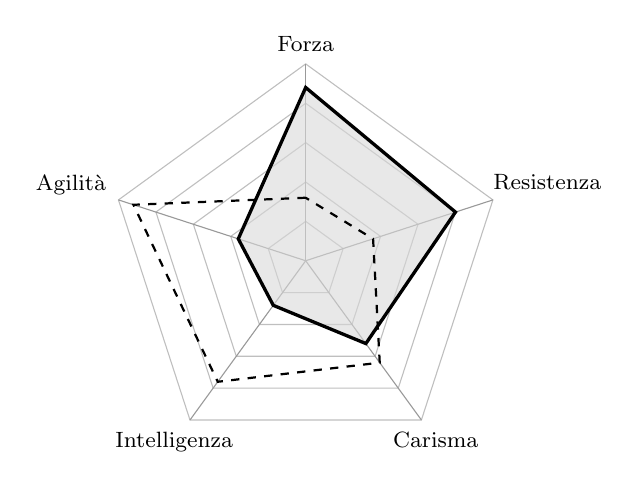
\begin{tikzpicture}[font=\footnotesize]
  \def\n{5}
  \foreach \r in {0.5,1,1.5,2,2.5} {
    \draw[black!25] (90:\r)
      \foreach \i in {1,...,4} { -- (90+\i*72:\r) } -- cycle;}
  \foreach \i/\lab in {0/Forza,1/Agilità,2/Intelligenza,3/Carisma,
                       4/Resistenza} {
    \draw[black!40] (0,0) -- (90+\i*72:2.5);
    \node[anchor=270+\i*72, inner sep=3pt] at (90+\i*72:2.55) {\lab};}
  \draw[very thick, fill=black!15, fill opacity=0.6]
    (90:2.2) -- (162:0.9) -- (234:0.7) -- (306:1.3) -- (18:2.0) -- cycle;
  \draw[thick, dashed]
    (90:0.8) -- (162:2.3) -- (234:1.9) -- (306:1.6) -- (18:0.9) -- cycle;
\end{tikzpicture}
\caption{Un grafico a radar con due profili di personaggio (valori
inventati): a colpo d'occhio si vede in quali categorie qualitative ciascuno
è spiccato.}
\label{fig:radar}
\end{figure}

\subsection{Il grafico a corde}

Nel \textbf{grafico a corde} (\emph{chord diagram}) ogni corda ha
un'\textbf{entrata} e un'\textbf{uscita}, indicata dalla punta della freccia.
L'esempio della slide mostra le \textbf{migrazioni globali} nel corso del
tempo.

\paragraph{Le relazioni tra sistemi.} Questo grafico è estremamente utile
quando si parla di \textbf{relazioni tra sistemi}. Si mettono a grafico tutti
i sistemi del gioco: il \emph{weather system}, il \emph{combat system}, gli
NPC, la vita sociale, e così via. Si mostra quanto sono collegati e in che
direzione (in un senso o in entrambi), e già a livello visivo si fa vedere
quanto, per esempio, il combattimento è collegato a tutto il resto, o quanto
un sistema invece è poco impattante e interessa relativamente meno. È un
altro modo per \textbf{mostrare} graficamente, invece di dover scrivere in
maniera esagerata, le relazioni tra i sistemi.

``Di grafici ce ne sono davvero tantissimi.'' Sta al designer imparare a
scegliere, come sempre, \emph{the right tool for the right job}; ``in questo
caso, \emph{the best tool for the right job}''.

% ---------------------------------------------------------------------
\section{La campagna di Russia in un grafico}
\label{sec:minard}

\subsection{Due avvertenze}

Per mostrare fin dove ci si può spingere, il docente ripropone un grafico già
intravisto, ``fichissimo, cioè per me è fichissimo'', con due avvertenze.
\begin{enumerate}
  \item Probabilmente lo si rivedrà al \textbf{terzo anno}, e verrà rifatta la
        stessa domanda: che cosa mostra? Ma il docente ``non cede di un
        passo'' e lo mostra lo stesso al primo anno, perché ``è troppo
        bello''. Al terzo anno, ``non mentite: noi lo sappiamo''.
  \item Il grafico è legato al \textbf{design}: fa parte di quel processo di
        \textbf{semplificazione} e di resa più grafica dei documenti di cui
        si sta parlando nelle lezioni di documentazione, e tornerà quando si
        parlerà di uno specifico tipo di documento, la ``summa'', il fine
        ultimo di questo processo.
\end{enumerate}

Il grafico viene attribuito a \textbf{Edward Tufte}, ``probabilmente il padre
delle infografiche'': ha dato i principi di base, alcuni dei quali sono
golden rules della documentazione (sezione~\ref{sec:golden-rules}), e sono
presi come base per fare UX e UI.\footnote{La mappa è in realtà opera
dell'ingegnere francese \textbf{Charles Joseph Minard} (1869). È stato Tufte,
in \emph{The Visual Display of Quantitative Information} (1983), a renderla
celebre, definendola probabilmente il miglior grafico statistico mai
disegnato.} Il docente darà poi il link a un talk che ne parla, ``uno dei
talk più belli che siano mai stati fatti sul design in generale, sul game
design in generale. A me ha aperto la mente.''

\subsection{Che cosa mostra?}

La regola del gioco: niente ``furia'', non si va a cercare che cos'è. Più ci
si spreme le meningi, più ritorno si avrà dopo. Si sa solo che è una
\textbf{variante del diagramma di Sankey}. E bisogna leggere il grafico, non i
testi (``sennò è troppo semplice'').

\begin{description}
  \item[Valerio] Potrebbe mostrare \textbf{scelte narrative} che proseguono
        con la storia. ``In questo caso no. Però è interessante: c'è un
        certo tipo di \textbf{progressione} in questo grafico.'' E, ammette il
        docente, ``ho mentito: sono due grafici'', uno sopra e uno sotto, che
        si legano tra loro.
  \item[Lorenzo] Sembra esserci una \textbf{correlazione} tra i due. La
        banda color ocra all'inizio è il 100\%; poi una parte si stacca, e
        nel tempo, procedendo, la quantità cambia, forse in un tempo comune
        alle due curve rappresentato da quella sotto. Nella banda nera si
        discrimina un'altra popolazione che si prende un'altra fetta. E
        quindi non sono percentuali ma \textbf{quantità}, perché nel tempo
        entrambe \textbf{diminuiscono}. ``Questo te lo confermo.'' Sembra uno
        strumento per analizzare più categorie e quantità correlate nel
        tempo. Il docente conferma la direzione: c'è una progressione,
        ``tra l'altro fisica''; la banda si rompe in quella nera, le
        quantità di entrambe diminuiscono, e c'è la correlazione con il
        grafico sotto, che è un \textbf{grafico a linea delle temperature}.
        Dalla classe si nota anche che la banda nera sembra ingrossarsi a
        spese dell'altra, e qualcuno azzarda un'ipotesi: petrolio bruciato e
        anidride carbonica emessa.
\end{description}

Il docente indica allora alcune linee sottili, ``con una forma che
sicuramente in vita vostra avete già visto''. Curve di livello? ``No, sono
troppo irregolari.'' Confini geografici? Una mappa delle temperature locali in
2D? Nessuno azzarda: sono \textbf{fiumi}.

\subsection{La risposta}

Il grafico mostra la quantità di uomini nell'\textbf{esercito di Napoleone
durante la campagna di Russia}, verso Mosca.
\begin{itemize}
  \item La banda chiara è la \textbf{marcia di andata}, quella nera la
        \textbf{ritirata}.
  \item La \textbf{larghezza} della banda è la grandezza dell'esercito.
  \item Durante la marcia alcuni se ne vanno: l'esercito si divide, alcuni
        tornano indietro, altri vanno avanti.
  \item In corrispondenza di un fiume si vede la banda assottigliarsi
        drasticamente: lì sono morti moltissimi uomini (``adesso io ci
        rido, ma non fa ridere'').
  \item Tutto in relazione alla \textbf{temperatura} in quei punti, che è il
        secondo grafico, sotto.
\end{itemize}

Per il docente ``è una figata'' perché, una volta letta la legenda,
\textbf{comunica immediatamente}, con un impatto grafico fortissimo, dove è
andato quell'esercito, che cosa ha vissuto, come si è piano piano non solo
separato ma anche \textbf{decimato} nel tempo: una campagna completamente
disastrosa. ``Con i grafici potete fare questa roba qua.''

\subsection{Dalle infografiche ai documenti}

In futuro si vedrà che lo stesso si può fare anche con la documentazione,
benché con i documenti di design sia veramente difficile: nella sua massima
espressione, \textbf{compressi in una singola pagina}. È il motivo per cui
Tufte è stato preso ad esempio e riadattato all'arte del documentare da
\textbf{Stone Librande}, il designer di \emph{Spore}, dei \emph{Sims} e di
altri titoli.\footnote{Nella trascrizione compare come ``Stanley Brandi''.
Il talk a cui il docente si riferisce è quasi certamente \emph{One-Page
Designs} di Stone Librande (GDC 2010), in cui la mappa di Minard e i principi
di Tufte sono il punto di partenza per i documenti di design di una sola
pagina.} Se ne riparlerà nella lezione di documentazione apposita. Non bisogna
raggiungere subito quel livello, ``perché è molto difficile, e non credo
nemmeno di esserci arrivato io''; ma il margine è tanto: \textbf{il tetto è
molto alto}. Si ragiona, si sperimenta, e si migliora nel tempo.

\paragraph{Approfondimento: Tufte nelle bibliografie di game design.} Tufte
compare nelle letture consigliate di entrambi i manuali del progetto.
Schell, in \emph{The Art of Game Design}, definisce \emph{The Visual Display of
Quantitative Information} ``la Bibbia (o almeno l'Antico Testamento) del
design delle interfacce grafiche'', e apre la sua lente della trasparenza
(\#62) con una citazione di Tufte: ``Per quanto bella sia la tua
interfaccia, sarebbe meglio se ce ne fosse di meno''. Brathwaite e Schreiber,
in \emph{Challenges for Game Designers}, consigliano \emph{Visual
Explanations}: per quanto si aderisca alle convenzioni di genere, sembra che
esistano solo uno o due modi di mostrare una barra della vita o il conteggio
delle munizioni; Tufte ``distrugge questa illusione'', mostrando molti modi
diversi di visualizzare un'informazione importante, con pregi e difetti di
ciascuno. È lo stesso messaggio della lezione: per ogni dato esiste un
grafico migliore degli altri, e trovarlo è parte del lavoro.

% ---------------------------------------------------------------------
\section{Principi per grafici migliori}
\label{sec:principi-grafici}

Ci sono comunque dei principi per migliorare, formattare e rendere più
visibili i dati di un grafico: le classiche regole della \textbf{Gestalt} e i
principi di design in generale. Cose che probabilmente si sanno già, ma è utile
ricordarle, e che si sono già cominciate ad applicare nella documentazione;
nei grafici le si può spingere ``all'esponenziale'', perché fare grafici è
``una pratica grafica, appunto''.
\begin{description}
  \item[Spazio negativo] Va sfruttato.
  \item[Scala] Ciò che è più grande impatta di più il lettore e viene
        percepito come più importante; ciò che è più piccolo, meno.
  \item[Gerarchia] L'ordine visivo delle informazioni.
  \item[Prossimità, forma, colore] Elementi vicini, della stessa forma o
        dello stesso colore vengono letti come un gruppo.
\end{description}

Al netto della ricerca (scoprire nuovi tipi di grafico, capire qual è il più
adatto) questa abilità si costruisce con l'\textbf{esperienza}: più grafici si
fanno, più si diventa abili, ``ancora di più rispetto alla documentazione
base, anche perché questo è documento''.

% ---------------------------------------------------------------------
\section{La matematica di base}
\label{sec:matematica-base}

\subsection{Quattro cose, da quinta elementare}

Non c'è tempo per un'altra pausa (``al massimo finiamo cinque minuti prima,
cosa che non è mai successa''), quindi si passa ai \emph{basic math
principles}. ``Qua siamo probabilmente in quinta elementare'': per chi non lo
sapesse non è un problema; le cose sono veramente quattro.

\subsection{La media}

La \textbf{media} (aritmetica) è la somma di tutti i numeri divisa per il
numero di elementi dell'insieme:
\[
  \bar{x} = \frac{x_1 + x_2 + \dots + x_n}{n} = \frac{1}{n}\sum_{i=1}^{n} x_i .
\]
``Su questo penso che nessuno abbia dei dubbi.''

\subsection{La media pesata}

Serve per alcuni framework o per alcuni calcoli in generale. Ci sono
\textbf{due modi} per farla.

\paragraph{Primo modo: pesi che sommano a uno.} Tutti i pesi sommati devono
dare \textbf{uno}, cioè il totale, il 100\%. Dati questi pesi, si
\textbf{moltiplica} ciascun valore per il rispettivo peso, ottenendo il valore
pesato, e poi si \textbf{somma}:
\[
  \bar{x}_w = \sum_{i=1}^{n} w_i\, x_i \qquad \text{con} \qquad
  \sum_{i=1}^{n} w_i = 1 .
\]

\paragraph{Secondo modo: pesi qualsiasi.} I pesi possono \textbf{non} dare il
100\%. Si moltiplica ciascun valore per il suo peso specifico, si sommano i
risultati, e la somma si divide per la \textbf{somma dei pesi}:
\[
  \bar{x}_w = \frac{\sum_{i=1}^{n} w_i\, x_i}{\sum_{i=1}^{n} w_i} .
\]
``Non è complessa, forse un passaggio in più.'' Il primo modo è un caso
particolare del secondo: se i pesi sommano a uno, il denominatore vale 1.

\paragraph{Un esempio.} Si vogliano confrontare due idee uscite dal
brainstorming dando un voto da 1 a 10 a tre criteri, con pesi diversi:
impatto (peso 3), costo contenuto (peso 2), coerenza con la visione
(peso 1). Un'idea con voti 8, 4 e 9 ha media semplice $(8+4+9)/3 = 7$, ma
media pesata
\[
  \frac{3\cdot 8 + 2\cdot 4 + 1\cdot 9}{3+2+1} = \frac{41}{6} \approx 6{,}83 .
\]
Con i pesi normalizzati ($3/6 = 0{,}5$; $2/6 \approx 0{,}33$;
$1/6 \approx 0{,}17$, che sommano a 1) si ottiene lo stesso risultato con il
primo modo. (L'esempio non è della lezione.)

\paragraph{Approfondimento: il valore atteso.} Schell (\emph{The Art of Game
Design}, capitolo~12) mostra uno degli usi più frequenti della media pesata
nel game design: il \textbf{valore atteso}, cioè la media di tutti i
risultati possibili di un'azione, pesati con la loro probabilità (pesi che,
come nel primo modo, sommano a uno). Se finendo su una casella verde si tira
un dado a sei facce e si ottengono altrettanti punti, il valore atteso è
$(1+2+3+4+5+6)/6 = 3{,}5$: è utile sapere che ogni volta, in media, si
guadagnano 3,5 punti. Con esiti non equiprobabili si pesa: tirando due dadi,
si vincono 5 dollari con un 7 o un 11 e se ne perde uno con qualsiasi altro
risultato. Le probabilità sono $6/36$ per il 7, $2/36$ per l'11 e $28/36$ per
il resto, quindi
\[
  \tfrac{6}{36}\cdot 5 + \tfrac{2}{36}\cdot 5 + \tfrac{28}{36}\cdot(-1)
  \approx 0{,}83 + 0{,}28 - 0{,}78 = 0{,}33 :
\]
alla lunga si vincono in media 33 centesimi a partita. Se vince solo il 7, il
valore atteso scende a zero (un gioco equo); se vince solo l'11, diventa
negativo ($-0{,}86$ circa). Schell ne fa una lente (\#35, \emph{The Lens of
Expected Value}): bilanciare un gioco passa spesso da conti di questo tipo.

\subsection{Le proporzioni}

L'ultima cosa è la \textbf{proporzione}: $a$ sta a $b$ come $c$ sta a $d$,
\[
  a : b = c : d ,
\]
dove $a$ e $d$ sono gli \textbf{estremi} e $b$ e $c$ i \textbf{medi}. La
proprietà fondamentale è che il prodotto dei medi è uguale al prodotto degli
estremi ($b \cdot c = a \cdot d$). Quindi:
\begin{description}
  \item[Incognita in un estremo] Si \textbf{moltiplicano i medi} e si divide
        per l'\textbf{estremo noto}. Esempio della lezione: in
        $100 : 35 = 20 : x$, i medi sono 35 e 20, l'estremo noto è 100:
        \[ x = \frac{35 \cdot 20}{100} = \frac{700}{100} = 7 . \]
        Verifica: 100 sta a 35 come 20 sta a 7.
  \item[Incognita in un medio] Si \textbf{moltiplicano gli estremi} e si
        divide per il \textbf{medio noto}. Esercizio della lezione: in
        $100 : 35 = x : 5$, gli estremi sono 100 e 5, il medio noto è 35. La
        classe risponde con il calcolo, ``500'', diviso 35:
        \[ x = \frac{100 \cdot 5}{35} = \frac{500}{35} \approx 14{,}3 , \]
        che il docente arrotonda a 14: 100 sta a 35 come (circa) 14 sta
        a 5.
\end{description}

``Avete tutte le informazioni basilari di matematica per sopravvivere alla
quinta elementare e al primo anno.''

\subsection{Che cosa verrà dopo}

Il discorso si complicherà al secondo anno, quando si parlerà di
\textbf{regressione lineare}: ma sono strumenti che servono per framework
specifici o per lavori specifici. Fare l'\textbf{economy designer} li
richiede, e anche un \textbf{data analyst} ha determinate competenze
matematiche; li si tratterà lì, punto per punto. Per ora interessa solo che
si ricordino queste quattro cose: semplici, ma ``una rinfrescata e averle lì
non vi fa male''.

% ---------------------------------------------------------------------
\section{Chiusura e prossimi appuntamenti}
\label{sec:chiusura-gd6}

La lezione è finita (``yes, abbiamo finito''), con un leggero margine di
anticipo. Il docente ricorda le scadenze:
\begin{itemize}
  \item il \textbf{production dictionary} per \textbf{lunedì 2}
        (sezione~\ref{sec:task-gd4});
  \item il \textbf{flowchart di Pac-Man} (o di \emph{Donkey Kong}) per
        \textbf{venerdì 6} (sezione~\ref{sec:task-gd6});
  \item l'altro task è già stato consegnato: il docente lo commenterà nel
        fine settimana o, al massimo, all'inizio della settimana successiva.
\end{itemize}

\paragraph{Leggere i commenti prima del 6.} Dopo che il docente avrà
commentato, bisogna \textbf{leggere i suoi commenti prima della lezione del
6}: in quella lezione si prenderà una pagina bianca e si comincerà a
documentare e a formattare la pagina insieme (sezione~\ref{sec:recap-documentazione}),
e prima di farlo è importante che il feedback ricevuto sia stato compreso.
Come detto l'altra volta, bisogna aspettare che il docente abbia commentato
tutto.

``Per lunedì portate il PC, perché Alessandro ne sarà sicuramente contento.''
I saluti sono di stagione: ``Buon Halloween! Buona festa dei morti!''

% ---------------------------------------------------------------------
\section*{Punti chiave del capitolo}
\addcontentsline{toc}{section}{Punti chiave del capitolo}

\begin{itemize}
  \item Nel \textbf{production dictionary} vanno i \textbf{nomi} unici o
        fraintendibili del gioco, spiegati in una o due righe (che cos'è una
        MT, che cos'è un tipo); il funzionamento profondo va nei documenti
        dedicati. Ordine alfabetico per leggibilità, ma le voci legate tra
        loro possono stare vicine; in ogni caso, \textbf{ordinato}.
  \item Nel brainstorming \textbf{nessuno viene fermato}, tutti parlano, si
        elenca tutto, si cercano background diversi. Un
        \textbf{facilitatore} (non un leader) fa sentire tutti ascoltati e
        tiene il brainstorming su uno scopo pratico. \textbf{Pause} e
        \textbf{cibo} riducono la tensione.
  \item Altre tecniche: circle, acting brainstorming, i \textbf{sei
        cappelli} di de Bono (partire dal verde; il nero è già giudizio),
        l'oggetto dal cappello, storyboard, domande, ``peggiore è, meglio
        è'', associative e \textbf{mind mapping}, il \textbf{TRIZ} (matrice
        di parametri, soluzione già nella cella, adatto a problemi
        fisici).
  \item Le regole di \textbf{Kawasaki} (make meaning, make mantra, next
        curve, DICEE, don't worry be crappy, hundred flowers, polarize,
        churn, niche, perfect your pitch) e lo \textbf{SCAMPER}. Il pitch si
        prova e riprova, ma \textbf{non si impara a memoria}.
  \item Dalle cento idee ad \textbf{almeno dieci}: \textbf{brainstorming
        matrix} impatto/effort, confronto, compromesso; contano anche la
        \textbf{motivazione} del team e la visione. Le idee vanno
        \textbf{distrutte}: se non si trova nessun difetto, c'è un problema.
  \item \textbf{KISS}: prototipare subito il cuore del gioco; muoversi,
        cambiare prospettiva, \textbf{rituali} che rompono la routine (il
        playtest del venerdì).
  \item Il \textbf{flowchart} è una rappresentazione grafica formalizzata di
        un processo; nasce nel software, e ai designer serve per IA,
        pipeline, game loop, sequenze di gameplay, player journey, UI.
        Serve a \textbf{mostrare invece di scrivere}.
  \item Regole: si legge \textbf{dall'alto in basso e da sinistra a
        destra}, nella direzione delle frecce; stesso livello, stessa
        gerarchia; il layout orizzontale evita il \textbf{wall of text}.
  \item Blocchi: \textbf{inizio/fine} (rettangolo arrotondato, obbligatori),
        \textbf{azione} (rettangolo), \textbf{decisione} (rombo, uscite
        sempre etichettate), \textbf{sotto-processo} (da spiegare in un altro
        flowchart), \textbf{input/output} (parallelogramma),
        \textbf{documento}.
  \item In un sistema o un loop di gioco il flusso \textbf{deve chiudersi o
        tornare indietro}: nessun ramo nel nulla. Le regole prima si
        imparano, poi si piegano (Oxenfree, il gioco di carte, Machinations,
        il behavior tree).
  \item Task: il \textbf{flowchart completo di Pac-Man} (Daniele:
        \emph{Donkey Kong}), come immagine leggibile e commentabile,
        esportata al 300--500\%, per venerdì 6.
  \item Grafici: \textbf{linea} per l'evoluzione continua e le previsioni,
        \textbf{gradini} per i salti discreti e le progressioni; barre e
        colonne (con legenda prima), istogrammi, torta e ciambella, aree,
        clustering; poi treemap, sunburst, \textbf{radar}, \textbf{corde}
        (relazioni tra sistemi) e la mappa di Minard resa celebre da Tufte.
        Il tetto è altissimo: fino ai documenti di una pagina di Librande.
  \item Matematica di base: \textbf{media}, \textbf{media pesata} (pesi che
        sommano a uno, oppure divisione per la somma dei pesi; il valore
        atteso ne è un caso), \textbf{proporzioni} (medi per medi, estremi
        per estremi).
\end{itemize}

%    \part{Laboratorio: le revisioni dei task}
%    \renewcommand{\thechapter}{R}
%    \renewcommand{\theHchapter}{R}   % solo con hyperref
%    % =====================================================================
%  Capitolo R — Gli errori nei task: revisioni, correzioni e consigli
%  del docente (capitolo "vivo", da aggiornare a ogni revisione)
%  Fonte: i documenti dei task consegnati dalla classe, con i commenti
%  di revisione di Mattia Podini (Google Docs esportati in .docx).
%  Task coperti finora:
%    T1  Arcade core elements  (revisioni del 28/10/2026, 9 documenti
%        di 8 studenti, circa 350 commenti)
%    T2  Production dictionary di un Pokémon (revisioni del 5-6/11/2026,
%        9 documenti di 9 studenti, 173 commenti del docente e 3 risposte
%        di studenti; .docx in tasks/revisionati/
%        2026-11-05_PokemonProductionDictionary/)
%    T3  TCG pain points, a gruppi (revisioni del 7/11/2026, 4 documenti
%        di 4 gruppi, 80 commenti; .docx in tasks/revisionati/
%        2026-11-07_TCGPainPoints/)
%    T4  Flowchart di Pac-Man (revisioni dell'11/11/2026, 8 consegne,
%        79 commenti: immagini commentate su Drive, PDF annotati e due
%        .docx; il task di Lorenzo in tasks/gd6-pacman-flowchart/)
%    T5  Compendium e High Vision di Metroid Dread (revisioni del
%        18/11/2026, 14 documenti di 7 studenti, 235 commenti; .docx in
%        2026_11_13_MDCompendium&HighVision/)
%    T6  Feedback ai concept art di Zoe, gioco di zombie (revisioni del
%        19/11/2026, 7 documenti, 113 commenti; il task di Lorenzo in
%        tasks/gd10-zombie-feedback/)
%
%  Pacchetti richiesti nel preambolo del libro: gli stessi di GD6
%    \usepackage[italian]{babel}, \usepackage[T1]{fontenc},
%    \usepackage[utf8]{inputenc} (solo pdfLaTeX), \usepackage{booktabs},
%    \usepackage{tikz} con le librerie di GD6 (qui servono
%    arrows.meta, positioning, calc). Nessun pacchetto nuovo.
%
%  Collocazione nel libro: una parte propria, in coda al corso, con
%  numerazione "R" (Revisioni):
%
%    \part{Il corso di Game Design}
%    ...
%    % =====================================================================
%  Capitolo 6 — Dal brainstorming ai flowchart: come si conduce un
%  brainstorming, flowchart, grafici e matematica di base
%  (problema e soluzione, terza e ultima parte; documentazione visiva)
%  Fonte: trascrizione della lezione GD6 (Game Design, primo anno)
%  Pacchetti richiesti nel preambolo del libro:
%    \usepackage[italian]{babel}, \usepackage[T1]{fontenc},
%    \usepackage[utf8]{inputenc} (solo pdfLaTeX), \usepackage{booktabs},
%    \usepackage{amsmath}, e in più, novità di questo capitolo:
%    \usepackage{tikz} con
%    \usetikzlibrary{shapes.geometric,shapes.symbols,shapes.misc,
%      arrows.meta,positioning,calc,fit}
%    (le librerie vanno caricate nel preambolo, non nel capitolo)
%  Nota sulla fonte: la trascrizione automatica storpia diversi nomi
%  propri (titoli, strumenti, autori) e contiene lunghi tratti ripetuti
%  in loop durante le due pause. Dove il riferimento è ricostruibile con
%  certezza lo si riporta nella forma corretta; dove non lo è, lo si
%  segnala in nota invece di indovinare. Le figure sono ricostruzioni
%  degli esempi mostrati a lezione (slide e lavagna draw.io), non copie.
% =====================================================================

\chapter[Dal brainstorming ai flowchart]{Dal brainstorming ai flowchart:
condurre un brainstorming, flowchart, grafici e matematica di base}
\label{cap:brainstorming-flowchart}

Con questo sesto capitolo si chiude, finalmente, la lunga lezione su
\emph{problema e soluzione} cominciata due capitoli fa
(capitolo~\ref{cap:problema-soluzione}) e proseguita nel precedente
(capitolo~\ref{cap:ricerca-idee}). Mancava l'ultima parte: \emph{come} si
conduce un brainstorming, con quali regole, quali tecniche e come si passa
da cento idee a una manciata di idee valutate. Chiusa quella, la giornata
cambia argomento e apre un blocco nuovo, dedicato agli strumenti
\textbf{visivi} della documentazione: i \textbf{flowchart}, i
\textbf{grafici} e quel poco di \textbf{matematica di base} che serve per
costruirli e leggerli.

La lezione, un venerdì pomeriggio a ridosso di Halloween, si tiene da remoto
ed è condotta ancora da Mattia Podini. Il percorso del capitolo ne ricalca la
struttura:
\begin{enumerate}
  \item le domande in apertura, ancora una volta sul \textbf{production
        dictionary} di Pokémon: che cosa si intende per
        \emph{nomenclatura}, come ordinare le voci, che cosa lasciare ad
        altri documenti (sezione~\ref{sec:pd-gd6});
  \item la conclusione della parte sul \textbf{brainstorming}: le condizioni
        per farlo bene, il \textbf{facilitatore}, le pause e il cibo
        (sezioni~\ref{sec:ripresa-gd6} e~\ref{sec:condurre-brainstorming});
  \item altre \textbf{tecniche} per generare idee, dai \emph{sei cappelli} al
        \textbf{TRIZ}, le regole dell'innovazione di \textbf{Guy Kawasaki} e lo
        \textbf{SCAMPER} (sezioni~\ref{sec:altre-tecniche}
        e~\ref{sec:kawasaki-scamper});
  \item come si passa \textbf{dalle cento alle dieci idee}: la
        \emph{brainstorming matrix}, il confronto, il tentativo di
        distruggere le proprie idee, il prototipo e le routine da spezzare
        (sezioni~\ref{sec:sortare-idee} e~\ref{sec:kiss-routine});
  \item i \textbf{flowchart}: che cosa sono, dove nascono, a che cosa servono
        a un designer, le regole di lettura, i blocchi, l'obbligo di chiudere
        il flusso, e una serie di esempi reali che le regole le piegano
        (sezioni~\ref{sec:flowchart-cosa}--\ref{sec:flowchart-esempi});
  \item il task della settimana: il \textbf{flowchart completo di Pac-Man}
        (sezione~\ref{sec:task-gd6});
  \item i \textbf{grafici}: un piccolo esercizio in aula (linea o gradini?),
        i grafici di base, quelli più ricchi e la mappa della campagna di
        Russia di Napoleone, ``uno dei grafici più belli mai fatti''
        (sezioni~\ref{sec:grafici-esercizio}--\ref{sec:principi-grafici});
  \item la \textbf{matematica di base}: media, media pesata, proporzioni
        (sezione~\ref{sec:matematica-base}).
\end{enumerate}

% ---------------------------------------------------------------------
\section{In apertura: ancora il production dictionary}
\label{sec:pd-gd6}

\subsection{Prima di cominciare}

L'avvio è il solito avvio di una lezione online: il docente non sente la
classe (``probabilmente perché non ho ancora condiviso lo schermo''), segna le
presenze, saluta chi entra. Poi il rituale: domande o dubbi sulla lezione
precedente, che oggi si conclude, o sui task in generale, ``anche perché il
production dictionary scade lunedì'' (il task del
capitolo~\ref{cap:problema-soluzione}, sezione~\ref{sec:task-gd4}).

\paragraph{Problemi di gameplay, prima di tutto.} La prima domanda riguarda
invece il task a gruppi sui \emph{pain point}
(sezione~\ref{sec:task-gd5}): i tre problemi principali trovati devono
riguardare il gameplay o possono toccare qualsiasi feature del gioco, per
esempio il negozio? Qualsiasi tipo di feature, chiaramente. Il docente però
\textbf{sconsiglia} di prendere un problema \textbf{artistico} o un problema
di \textbf{performance}: se davvero non si trova altro, lo si può includere
come punto finale, ma la priorità va ai \textbf{problemi di gameplay}.

\subsection{Che cosa si intende per nomenclatura}

Mattia, uno studente, confessa di non aver ancora capito la consegna del
production dictionary. Ha provato a lavorarci in una cartella personale, ma
si è accorto che stava scrivendo e \emph{spiegando meccaniche}, e ha il
sospetto che non sia quello che viene chiesto. ``Che cosa si intende per
nomenclatura?''

Il docente ricorda di averlo già ripreso all'inizio della lezione precedente
(sezione~\ref{sec:pd-ripreso}) e lo rispiega. L'obiettivo è spiegare
\textbf{nomi unici legati al gioco}, o alla produzione del gioco. Possono
essere nomi di meccaniche, e nel caso di Pokémon lo possono essere
tranquillamente; ma più spesso sono nomi che spiegano un oggetto del mondo,
un \emph{game object} del mondo di Pokémon. L'esempio è il \textbf{tipo} (o
elemento): si spiega che cosa sono i vari tipi, che cos'è il tipo di un
Pokémon.

\paragraph{Che cosa \emph{non} ci va.} Negli esempi mostrati nelle slide,
come la voce \emph{Chase} (lo stato di inseguimento di un'intelligenza
artificiale, sezione~\ref{sec:production-dictionary}), è chiaro che quello
stato non verrà spiegato in un documento dedicato solo a lui: sarà spiegato
nel documento delle IA. Lì si trovano le spiegazioni \textbf{profonde}: come
funziona la meccanica, che parametri ha, che cosa richiede lato
programmazione, lato arte e così via. Nel production dictionary finisce
invece \textbf{a che cosa è legato quel nome}, a livello descrittivo: una o
due righe, una descrizione succinta. Lo scopo è che il lettore, di qualunque
natura sia (artista, grafico, programmatore, designer), sappia \textbf{a che
cosa si riferisce quella parola}.

\paragraph{La webcam, per favore.} A metà spiegazione il docente chiede a
Mattia di accendere la webcam: ``già faccio fatica a leggere naturalmente i
volti delle persone, figuriamoci se non ti vedo''; vuole capire se la
spiegazione arriva o no. Il problema dello studente era proprio questo:
quando si metteva a scrivere, gli veniva spontaneo descrivere le meccaniche,
non le nomenclature.

\subsection{Priorità: un limite di una pagina}

Per tutto ciò che è estremamente specifico si fa riferimento ai
\textbf{singoli documenti}. E gli studenti hanno anche il limite di
\textbf{una pagina}, quindi devono per forza scegliere le nomenclature
\textbf{più importanti} del gioco. Con molto più spazio si potrebbe discutere
se spiegare meccaniche uniche, specifiche, o qualcosa di estremamente
laterale.

\paragraph{Un caso limite.} Spiegare una singola mossa molto particolare è un
caso estremamente unico,\footnote{Nella trascrizione la mossa compare come
``fuoco-bomba''; non è chiaro a quale mossa o meccanica ci si riferisca.
L'esempio vale comunque come caso estremamente specifico.} ben diverso dallo
spiegare, per esempio, che cos'è una \textbf{MT} o una \textbf{MN}. E anche
per le MT conviene separare due piani:
\begin{itemize}
  \item \textbf{come funziona il sistema}: se una MT è consumabile o no,
        quante mosse ci sono e così via; questo può essere relegato ad altra
        documentazione;
  \item \textbf{che cos'è}: questo sì, è materia da dizionario.
\end{itemize}
Ancora più a monte si potrebbe spiegare che cos'è un \emph{oggetto} di gioco,
un item della borsa; ma ``oggetto'' è abbastanza comprensibile. L'ultima
parola spetta agli studenti, ma il criterio del docente è questo: si parla di
\textbf{nature uniche del gioco}, oppure \textbf{fraintendibili}. È questa
l'utilità del documento.

\paragraph{Non è un errore, è un'altra scelta.} Quello che allo studente
veniva istintivamente da fare non è sbagliato di per sé: rispetto alla
consegna è un'altra cosa, ma dal punto di vista della produzione non è un
errore. Come detto l'ultima volta, il production dictionary si può
\textbf{ibridare} con altri documenti (sezione~\ref{sec:pd-ripreso}): lo si
può mettere all'inizio di un documento, oppure spiegare le singole
terminologie in un GDD o in un altro tipo di documentazione, e allora quello
è il documento che spiega quella meccanica. Se il gioco \textbf{non ha un
grande rischio di fraintendimento}, si può anche valutare di avere un
documento a sé che funge da dizionario: non è obbligatorio.

\subsection{Raggruppare o ordinare alfabeticamente?}

Intanto Lorenzo ha la webcam spenta: ``vedo che Lorenzo si è affondato
nell'erba alta ed è diventato un Pokémon''. La parola passa a Valerio, che
ha stilato una serie di elementi e, siccome erano tanti, li ha
\textbf{raggruppati per fili comuni}. È sbagliato?

Dipende dal numero, dalla mole di informazioni che si danno al lettore. Su
una pagina sola può funzionare; quale sia la scelta ideale il docente non
può dirlo (``sennò poi dopo me la modificate''). Ma il ragionamento è
questo, esattamente come per un dizionario:
\begin{itemize}
  \item la \textbf{maggior leggibilità}, nel vuoto, ce l'ha l'\textbf{ordine
        alfabetico};
  \item l'ordine alfabetico però non risolve un problema: alcune
        nomenclature sono \textbf{legate ad altre}. L'esempio, forse un
        azzardo, è \emph{Pokémon} e \emph{Poké Ball}: al lettore potrebbe
        essere utile sapere prima l'informazione più rilevante e subito
        dopo quella associata.
\end{itemize}
Nel caso degli studenti può contare meno; in production dictionary
esageratamente grossi conta di più. In ogni caso, se il production dictionary
c'è (e non è una necessità averlo nella produzione), \textbf{deve essere
ordinato}.

\paragraph{I problemi di stato.} Valerio ha anche parlato delle lotte,
elencando e descrivendo tutti i \textbf{problemi di stato}: dovrebbero stare
in un documento a parte, dedicato alle lotte? ``Posso fare un esempio?''
``Certo che puoi farlo, però io poi sarò libero di non risponderti.'' È più
un problema di \textbf{priorità sulle nomenclature}; sul fatto di avere un
documento a parte o meno, il docente preferisce non rispondere adesso: se ne
riparlerà dopo che avrà commentato il documento.

Una piccola nota di colore chiude il giro: Mattia non sa come abbassare la
mano su Zoom. ``Non sono lo Zoom guru, quindi figurati.''

% ---------------------------------------------------------------------
\section{Dove eravamo rimasti}
\label{sec:ripresa-gd6}

\subsection{La forbice che si allarga}

Se non c'è altro, si conclude la lezione su problema, idea, ricerca e
brainstorming. L'ultima volta ci si era fermati quasi alla fine: manca
la parte sulle \textbf{metodologie per fare brainstorming}.

Il docente ricorda una cosa che vale per tutta la lezione: più si va avanti,
dall'inizio verso la fine, più \textbf{la forbice si amplia}.
\begin{description}
  \item[Nella ricerca] non ci sono limiti, ma c'è almeno una struttura: una
        forma dei dati, delle priorità (target audience, competitor e così
        via). Dare priorità è soprattutto una questione di
        \textbf{tempistiche}: in pre-produzione il tempo sarà poco e ci sarà
        tanto da fare, quindi quanto più si riesce a coprire di quella lista
        non omnicomprensiva (la mappa della ricerca,
        sezione~\ref{sec:mappa-ricerca}), meglio è. Alcune cose andrebbero
        fatte subito: i \textbf{competitor}, fondamentali, e
        l'\textbf{utente}, più di tutti; anche il \textbf{mercato} è
        importante. Le priorità ci saranno per forza, perché il tempo non è
        infinito. E per la ricerca strutture e framework ce ne sono, e sono
        abbastanza codificati: la lista vista (le Liberating Structures),
        la SWOT analysis, la perceptual mapping
        (sezione~\ref{sec:perceptual-mapping}).\footnote{Nella trascrizione
        compaiono come ``la lista di pesciola'' (verosimilmente un
        riferimento storpiato alla lista delle Liberating Structures,
        sezione~\ref{sec:problema-necessita}) e ``swap analysis'', che è
        quasi certamente la SWOT analysis (\emph{Strengths, Weaknesses,
        Opportunities, Threats}).}
  \item[Nell'ideazione] e nel brainstorming le tecniche ci sono, ma il campo
        è \textbf{probabilmente infinito}. Si può adottare più o meno
        quello che si vuole, soprattutto a seconda del gruppo che fa
        brainstorming: non è detto che ci sia l'intero team, magari solo il
        team di design, o un \emph{feature team} all'interno del team di
        design. A seconda di chi si è nel team e di quanto è grande, si può
        davvero fare quello che si vuole: ``potete giocare a freccette,
        far venire in mente le idee, o giocare a biliardo, davvero
        qualsiasi cosa funziona''.
\end{description}
Va bene tutto, \textbf{fintanto che porta un risultato}: quella
``fantomatica'' ideazione di \textbf{cento idee} da \emph{sortare} e scartare
(sezione~\ref{sec:principi-brainstorming}).

% ---------------------------------------------------------------------
\section{Come si conduce un brainstorming}
\label{sec:condurre-brainstorming}

\subsection{Le condizioni}

Ci sono però alcune condizioni importanti.

\paragraph{Nessuno viene fermato.} Durante il brainstorming, cioè nel momento
in cui si generano le idee, \textbf{nessuno deve essere fermato} dal
generarle. Non si scartano subito potenziali idee che ``non c'entrano
nulla'': \textbf{le si elenca tutte}. Poi, eventualmente, ci sarà una fase,
insieme o da soli, in cui queste idee vengono \textbf{filtrate}.

\paragraph{Tutti devono poter parlare.} Tutti devono sentirsi nella
condizione di dire la propria e di far crescere quella grande lista di idee,
che alla fine dei conti è l'obiettivo: buttare giù davvero qualsiasi cosa.
Anche perché quello che verrà scartato può ritornare in un'altra forma, in
un'altra maniera, o anche solo far scaturire qualche idea nuova per
implementazioni future. Qualsiasi spunto è utile: lasciare la parola a
tutti, e nella fase di brainstorming \textbf{qualsiasi cosa va bene}.

\paragraph{Non solo designer.} Sempre per arrivare a una quantità maggiore,
e potenzialmente più \textbf{diversificata}, di idee, conviene avere nel
brainstorming \textbf{non solo designer}, o comunque non solo persone con lo
stesso background. A seconda di quanto sono disponibili e di quanto sono
dentro l'industria, si cercano \textbf{punti di vista diversi}: l'obiettivo è
ampliare la propria visione il più possibile.

\subsection{Il facilitatore}

Questo vale sicuramente per i team grossi, ma va valutato anche per quelli
piccoli, soprattutto le prime volte, se c'è difficoltà a parlare o se si è
meno portati a rompere il ghiaccio o a essere espansivi: conviene avere un
\textbf{facilitatore}. Non un leader, ma qualcuno che si preoccupa di
\textbf{controllare il flusso} del brainstorming: quanto tempo si sta
spendendo a discutere di un'idea, o ``a tirare quella freccetta''.

Il facilitatore ha fondamentalmente \textbf{due obiettivi}:
\begin{enumerate}
  \item \textbf{assicurarsi che tutti stiano bene} durante il brainstorming.
        A livello pratico vuol dire che tutti parlino e abbiano lo stesso
        tempo per parlare; ma c'è un passo in più, che tutti si sentano
        \textbf{a proprio agio}. Garantire la parola a tutti non basta
        necessariamente: a seconda dei membri del team, e di quanto li si
        conosce, l'obiettivo è \textbf{farli sentire ascoltati};
  \item \textbf{assicurarsi che il brainstorming abbia uno scopo pratico}.
        Fare brainstorming ``è una figata, piace a tutti'', ma il rischio
        di ``buttarla in caciara'' è molto grosso. È bello avere un momento
        di comunione con il team, più o meno regolamentato; tuttavia
        \textbf{bisogna quagliare}, arrivare a una lista lunga e concreta di
        idee. Il facilitatore si chiede quanto tempo va dedicato al
        brainstorming (un'ora?), controlla che si stia andando nella
        direzione corretta ed eventualmente \textbf{tira le redini} se
        qualcuno sta divagando.
\end{enumerate}

\paragraph{Approfondimento: chi deraglia, rimette sui binari.} Schell, tra i
suoi sedici consigli pratici per il brainstorming (\emph{The Art of Game
Design}, capitolo~7), incoraggia a \textbf{fare battute}: le battute
sciolgono la mente e fanno vedere le cose da prospettive che si erano perse,
ed è dalle prospettive nuove che nascono le grandi idee. Ma avverte che,
soprattutto in gruppo, le battute possono portare fuori strada; uscire dai
binari ogni tanto va bene (``le idee buone potrebbero non essere sui
binari''), purché ci si prenda la responsabilità di rientrarci. Il suo
comandamento è: \emph{he who derails, rerails}, chi fa deragliare rimette sui
binari. È, in piccolo, il secondo compito del facilitatore distribuito su
tutti i partecipanti.

\subsection{Pause e cibo}

\paragraph{Fare delle pause.} Conviene avere \textbf{pause tra una fase e
l'altra}. Al secondo anno si parlerà meglio di come affrontare la produzione,
di come lavorare con altri esseri umani, dell'importanza delle soft skill;
cose importanti, che il docente non vuole sminuire, ma il primo anno è il
campo di prova. Le pause servono a ridurre ``il cortisolo, mettiamola
così'': evitare che le persone impazziscano o che comincino a percepirsi
\textbf{screzi} forti tra gli individui.

È il discorso precedente visto dall'altro lato: se non si fa parlare tutti,
e soprattutto se qualcuno comincia a \textbf{smontare le idee}, o fa già la
fase di prendere un'idea e buttarla subito fuori dal cesto perché non ha
senso con i limiti, con la visione o con quello che si vuole, qualcuno
potrebbe ``inalberarsi'', prenderla male. E si ammetta pure che il team sia
grosso e che ci siano già delle inimicizie al suo interno.

\paragraph{Portate il cibo.} Per risolvere questo problema: pause, e poi
\textbf{cibo}. Lo si vedrà in modo più strutturato al secondo anno, ma il
mantra è: ``portate il cibo, portate la pizza. Non lo so, quello che
mangiano gli esseri umani generici. Io non mangio la pizza, però\dots''.
Generalmente avere delle pause in cui si mangia e si beve \textbf{aiuta
notevolmente a ridurre la tensione}.

% ---------------------------------------------------------------------
\section{Altre tecniche per generare idee}
\label{sec:altre-tecniche}

\subsection{Una lista, non un programma}

I modi per fare brainstorming, per generare idee in generale, sono tanti. Il
docente non li vede tutti punto per punto, ma li elenca; si aggiungono a
quelli già visti nel capitolo precedente (sezione~\ref{sec:tecniche-idee}).

\subsection{Circle}

Ci si mette \textbf{in cerchio}, si scrive una parola, si va avanti. Si
comincia con, per esempio, il tipo di gioco, una \emph{game quality}, un tema,
un'emozione; si passa il foglietto alla persona successiva, che aggiunge
un'altra parola, e così via finché il giro non è finito. A volte si fanno
più giri. È un modo per \textbf{ibridare la propria idea iniziale con
quelle degli altri} e vedere che cosa esce.\footnote{Il docente lo associa,
``se non sbaglio'', a un gioco dei futuristi. Il meccanismo descritto
(ciascuno aggiunge un pezzo senza controllare l'insieme) ricorda piuttosto il
\emph{cadavre exquis} dei surrealisti.}

\subsection{Acting brainstorming}

Si \textbf{mette nei panni di un'altra persona}: nella slide, una persona
famosa, un personaggio famoso. Ma vale anche, più in generale, per mettersi
nei panni di qualcun altro: avere la capacità \textbf{empatica} di vedere come
si è percepiti dall'altra parte, o che cosa si potrebbe provare dall'altra
parte.

\paragraph{Fuori dal brainstorming.} Il concetto è utile ben oltre la fase di
brainstorming. Un esempio: un 3D artist o un concept artist consegna i suoi
concept e gli vengono rimandati indietro, ogni volta, per una determinata
ragione. È ovvio, o almeno molto probabile, che il suo \textbf{morale} si
riduca. Mettersi nei suoi panni aiuta; poi bisognerà capire perché succede e
come risolverlo. Mettersi nei panni dell'altro aiuta a spiegare alcune
problematiche della produzione e del team: il morale basso, una persona che
non è mai presente o che non parla mai durante i meeting. Come sempre, si
cerca di arrivare alla \textbf{radice del problema}
(sezione~\ref{sec:problema-necessita}).

\subsection{I sei cappelli}

I \textbf{sei cappelli} vengono da un libro\footnote{\emph{Six Thinking Hats}
di Edward de Bono (1985), noto in italiano come \emph{Sei cappelli per
pensare}.} e possono essere utili per diversi tipi di attività. Ogni cappello
ha una \textbf{durata specifica} a seconda dell'attività ed è associato, un
po' come nell'acting brainstorming, alla necessità di guardare o di agire da
un determinato punto di vista:
\begin{description}
  \item[Blu] la \emph{big picture}: si guarda il problema ad alto livello;
  \item[Bianco] fatti e informazioni: si guardano i fatti, i dati;
  \item[Rosso] più istintivo: \emph{feelings and emotions};
  \item[Nero] il \textbf{giudizio critico}. Questo \textbf{rompe la fase di
        brainstorming}: è utile quando si comincia già a \emph{sortare} le
        idee, ``senza ciarle'';
  \item[Giallo] estremamente positivo: ``yes'', sorriso ``a 34 denti'', si va
        avanti;
  \item[Verde] le \textbf{idee nuove}.
\end{description}
È chiaro quindi che la fase di brainstorming dovrebbe partire col
\textbf{verde}, e comunque avere tanti momenti ``col cappello verde''. A volte
si passa da una fase all'altra; la lista completa è nel libro, che non è
necessario leggere, ma si trova anche in giro.

\subsection{L'oggetto dal cappello}

``Questo piace particolarmente a Diego'', il direttore del corso, e serve a
mostrare ancora una volta che nel generare idee si può infilare dentro
qualsiasi cosa. Si sfruttano \textbf{oggetti particolari, gadget}, pescati da
un ``fantomatico'' cappello, e si fa brainstorming su quell'oggetto: che cosa
c'entra, e come può aiutare a risolvere il problema. ``Utile? Non lo so, io
non l'ho mai usato, però sta qua.''

\paragraph{Approfondimento: i giocattoli sul tavolo.} Schell propone qualcosa
di molto simile tra i suoi consigli per il brainstorming
(\emph{The Art of Game Design}, capitolo~7, \emph{Toys}): portare al tavolo
dei giocattoli, alcuni legati al problema e altri che non c'entrano niente.
Il suo paragone sono i ristoranti pieni di oggetti strani alle pareti: non
sono decorazione, sono spunti di conversazione. I giocattoli coinvolgono la
creatività anche in modo \textbf{tattile}; e se si porta un po' di
plastilina per modellare le idee, ``sembra stupido, ma la creatività è
stupida''.

\subsection{Storyboard}

Lo \textbf{storyboard} è un po' come il \emph{drawing}
(sezione~\ref{sec:tecniche-idee}): non importa saper disegnare bene o male,
importa che sia \textbf{chiaro}, anche con gli stickman. Si disegna il
processo, una potenziale storia che spieghi l'idea, che la ``metta a terra''
nel brainstorming.

\subsection{Le domande}

\textbf{Domande}: ci si butta dentro più domande possibili, su qualsiasi
cosa. È anche un modo, più o meno serio, per iniziare quel tipo di
``sortaggio'' (``non sorteggio, sortaggio''), cioè di \textbf{valutazione}
delle idee messe a terra.

\subsection{Papà e mamma: peggiore è, meglio è}

Un'altra tecnica importante è presentata nelle slide con una metafora
familiare: da una parte il \emph{papà}, la figura particolarmente
\textbf{pragmatica}; dall'altra la parte in cui ci si butta dentro davvero
qualsiasi cosa e va bene. Anzi: \textbf{peggiore è l'idea, meglio è},
almeno teoricamente. Sempre nell'idea che \textbf{tutto può aiutare}, e che
la soluzione si può trovare partendo da qualsiasi cosa.\footnote{La
trascrizione non permette di ricostruire con certezza il nome della tecnica
nella slide. L'impostazione (cercare deliberatamente le idee peggiori) è
quella nota come \emph{worst possible idea} o \emph{reverse brainstorming}.}

\paragraph{Approfondimento: scrivere tutto, anche le idee stupide.} Schell
(\emph{The Art of Game Design}, capitolo~7, \emph{Write Everything}) cita
Linus Pauling: ``il modo migliore per avere una buona idea è avere molte
idee''. Il suo consiglio è di non aspettare l'idea brillante ma di scrivere
\textbf{tutto} ciò che è anche solo lontanamente collegato al problema, ogni
idea stupida che passa per la testa: bisogna far uscire quelle stupide prima
che comincino ad arrivare quelle buone, e a volte un'idea stupida diventa
l'ispirazione per un'idea geniale. Non ci si censura, e soprattutto in
gruppo non si censurano gli altri: ``le loro idee stupide valgono quanto le
tue''.

\subsection{Associative e mind mapping}

Con l'\textbf{associative} si parte da una parola e le si associano parole
simili. Si può usare anche un \emph{word association tool}, un'IA o
qualsiasi software che associa parole.

È molto simile al \textbf{mind mapping}, che si vede di solito: ``sicuramente
l'avrete vista da qualche parte''. Quando si parla di brainstorming, la
visione pratica è generalmente questa: una \textbf{grande mappa sulla
lavagna}, che tutti devono poter vedere. Si parte da un concetto, si
dividono i rami per \textbf{categorie}, e i rami grossi portano a rami più
piccoli, con parole o concetti sempre legati alla categoria principale
(figura~\ref{fig:mind-map}).

\begin{figure}[htbp]
\centering
\begin{tikzpicture}[
    font=\small,
    centro/.style={ellipse, draw, thick, minimum width=2.6cm,
                   minimum height=1cm, align=center},
    ramo/.style={rectangle, rounded corners=3pt, draw, align=center,
                 minimum height=0.7cm, inner sep=4pt},
    foglia/.style={align=center, inner sep=2pt, font=\footnotesize},
    every edge/.style={draw}]
  \node[centro] (c) {Gioco sul\\viaggio nel tempo};
  \node[ramo] (m) at (-4.2,1.6) {Meccaniche};
  \node[ramo] (t) at (4.2,1.6) {Tema};
  \node[ramo] (e) at (-4.2,-1.6) {Emozioni};
  \node[ramo] (p) at (4.2,-1.6) {Pubblico};
  \draw[thick] (c) -- (m); \draw[thick] (c) -- (t);
  \draw[thick] (c) -- (e); \draw[thick] (c) -- (p);
  \node[foglia] (m1) at (-6.3,2.6) {riavvolgere};
  \node[foglia] (m2) at (-6.4,1.0) {loop};
  \node[foglia] (m3) at (-3.0,2.7) {paradosso};
  \draw (m) -- (m1); \draw (m) -- (m2); \draw (m) -- (m3);
  \node[foglia] (t1) at (6.3,2.6) {orologi};
  \node[foglia] (t2) at (6.4,1.0) {rovine};
  \node[foglia] (t3) at (3.0,2.7) {nostalgia};
  \draw (t) -- (t1); \draw (t) -- (t2); \draw (t) -- (t3);
  \node[foglia] (e1) at (-6.3,-2.6) {rimpianto};
  \node[foglia] (e2) at (-6.4,-1.0) {sorpresa};
  \node[foglia] (e3) at (-3.0,-2.7) {ansia};
  \draw (e) -- (e1); \draw (e) -- (e2); \draw (e) -- (e3);
  \node[foglia] (p1) at (6.3,-2.6) {puzzle lover};
  \node[foglia] (p2) at (6.4,-1.0) {sessioni brevi};
  \node[foglia] (p3) at (3.0,-2.7) {mobile};
  \draw (p) -- (p1); \draw (p) -- (p2); \draw (p) -- (p3);
\end{tikzpicture}
\caption{Struttura tipica di una mind map: un concetto centrale, rami
principali per categoria e rami secondari sempre legati alla categoria da
cui partono. Il contenuto è un esempio inventato.}
\label{fig:mind-map}
\end{figure}

\paragraph{Che cosa usare per il task.} Per il task in corso
(sezione~\ref{sec:task-gd5}) il mind mapping funziona molto bene, ma possono
funzionare anche l'associative o il circle. Questi, i più
\textbf{immediati}, sono quelli che il docente consiglia al momento.

\paragraph{Approfondimento: lo spazio ricorda.} Due consigli di Schell
(\emph{The Art of Game Design}, capitolo~7) spiegano perché la mappa sulla
lavagna funziona. Il primo (\emph{The Writing on the Wall}): in gruppo serve
una superficie che tutti vedano contemporaneamente; Schell preferisce grandi
fogli adesivi o carta da pacchi alle pareti, che si possono riposizionare,
staccare, arrotolare e conservare, per riprendere un anno dopo il
brainstorming ``come se non si fosse mai interrotto''. Il secondo
(\emph{The Space Remembers}, espressione presa da Tom Kelley): la memoria per
le liste è scarsa, ma quella per la \textbf{posizione} delle cose intorno a
noi è ottima; appendere le idee nella stanza aiuta a ritrovarle e a vederne
le connessioni. Un terzo consiglio è più sorprendente
(\emph{Number Your Lists}): \textbf{numerare} le liste le rende più facili da
discutere (``mi piacciono dalla 3 alla 7'') e, stranamente, dà alle voci una
certa dignità, così che vengono prese più sul serio.

\subsection{TRIZ}
\label{sec:triz}

Il \textbf{TRIZ}, già accennato (sezione~\ref{sec:tecniche-idee}), viene
solo ``accennato'' anche qui, perché è estremamente complesso. Nasce
nell'\textbf{Unione Sovietica}. Il concetto è un po' quello dell'astrazione
vista nel SIT, il \emph{closed world}: il problema, per come viene
formulato, contiene già la soluzione. Anzi, \textbf{non trovare la soluzione
dipende dal fatto che il problema non è formulato correttamente}. La
soluzione è già lì; per arrivarci bisogna \textbf{astrarre il problema},
trovare \textbf{soluzioni astratte} e poi \textbf{concretizzarle}. ``Questo è
il salto.''

\paragraph{Come funziona.} Il TRIZ nasce dall'analisi di un numero enorme di
\textbf{brevetti} sovietici, in cui il comune denominatore era astrarre i
problemi e vedere come erano stati risolti. Problemi e soluzioni vengono
messi in una \textbf{matrice} con righe e colonne: sulle righe e sulle
colonne ci sono le stesse \emph{feature}, da 1 a $n$ (``sono 40, se non
sbaglio, forse sono state anche aumentate nel
tempo'').\footnote{Nella formulazione classica di Genrich Altshuller la
\emph{matrice delle contraddizioni} incrocia 39 parametri tecnici (righe:
il parametro che si vuole migliorare; colonne: quello che peggiora di
conseguenza), e ogni cella suggerisce alcuni dei \textbf{40 principi
inventivi}. Versioni successive (come la \emph{Matrix 2003}) hanno esteso i
parametri. Nella trascrizione il nome compare come ``Drizzt'', ``TRIPS'' e
``TRIZZE''.} Le feature possono essere il peso di un oggetto in movimento,
il peso di un oggetto stazionario, la lunghezza di un oggetto in movimento,
la lunghezza di uno stazionario, l'area di un oggetto in movimento, e così
via.

Se si riesce ad astrarre il proprio problema e a trovare la riga e la
colonna su cui si fonda, si va a cercare la \textbf{cella} che le combina.
Un esempio: il problema è mantenere caldo il contenuto di un bicchiere
\textbf{senza far scottare le mani} di chi lo tiene. Il calore fa parte di
quel tipo di feature: si cerca la cella che combina la colonna e la riga del
problema.

\paragraph{Piegarsi alle regole.} Il TRIZ si basa principalmente su
\textbf{problemi meccanici}, e non è facile. La soluzione, se si usa il TRIZ,
\textbf{deve derivare da quello che viene consigliato nella cella}: per
usarlo non basta conoscerlo, bisogna anche piegarsi alle sue regole. Può
essere un buon modo, se ci si leggono righe e colonne, soprattutto per
\textbf{problemi pratici di produzione fisica}: per esempio nei giochi da
tavolo, dove la stampa, la grandezza o il costo di una componente è
eccessivo. Ma resta estremamente codificato: è tra le cose che si possono
approfondire.

% ---------------------------------------------------------------------
\section{Le regole di Kawasaki e lo SCAMPER}
\label{sec:kawasaki-scamper}

\subsection{Le regole dell'innovazione di Guy Kawasaki}

Le \textbf{regole di Kawasaki} non vengono viste nel dettaglio: i punti sono
segnati nella slide, per andare veloci, e chi vuole può guardare il video,
``classico video di TEDx, informativo fino a un certo
punto''.\footnote{Guy Kawasaki, \emph{The Art of Innovation}, TEDxBerkeley,
2014. Nella trascrizione diversi titoli delle regole sono storpiati
(``Con la nice people'', ``Charm baby charm'', ``Nishita e Sensor'',
``Dot worried e crappy''); qui sono riportati nella forma originale.}
Alcune cose sono già state viste. Il docente le commenta così:
\begin{description}
  \item[Make meaning] (e non soldi). Se l'obiettivo è questo, l'obiettivo è
        portare \textbf{innovazione}; poi arriva il guadagno. Però non è
        detto: va valutato attentamente.
  \item[Make mantra] Può essere utile durante il \textbf{pitch}: servono frasi
        che catturino l'audience o che facciano capire il prodotto in poche
        parole.
  \item[Jump to the next curve] Far \textbf{evolvere} la propria idea:
        iterare, ma in positivo, sempre in modo migliorativo.
  \item[Roll the DICEE] Creare qualcosa di elegante, completo, profondo,
        intelligente, non semplice.\footnote{L'acronimo di Kawasaki è
        DICEE: \emph{deep, intelligent, complete, empowering, elegant}.} Lo si
        può paragonare al \textbf{design elegante}
        (sezione~\ref{sec:design-elegante}) che, ripete il docente, non è
        sempre necessario, ma ``è lì''.
  \item[Don't worry, be crappy] Creare \textbf{prototipi}: arrivarci il prima
        possibile e \textbf{non avere paura di fare schifo}.
  \item[Let a hundred flowers blossom] Lasciare che \textbf{nuove dinamiche}
        emergano. Applicato ai videogiochi: che emergano nuove meccaniche, o
        che i giocatori vedano e usino in modo diverso le cose che si erano
        previste. Con il \textbf{playtest} si valuta se il giocatore fa
        qualcosa a cui non si era pensato, che non si pensava possibile, e se
        ha senso all'interno della propria visione. Generalmente
        assecondare l'utente quando legge qualcosa a modo suo (ammesso che
        sia il proprio target audience) è positivo: non sempre, ma nella
        stragrande maggioranza dei casi. Il controllo del progetto resta però
        al team: è il team a decidere \textbf{se quel bug diventa una feature
        o no}.
  \item[Polarize people] Se ne riparlerà nella lezione sul feedback, ma se ne
        è già cominciato a parlare. Le persone, statisticamente, su un
        argomento si distribuiscono su una \textbf{curva a campana}.
        Interessa capire chi sono gli \textbf{estremi}: chi ama alla follia
        il gioco e chi, invece, ``vi vuole sgozzare''. Va bene \textbf{non
        creare il prodotto per queste persone}; ma sapendo che cosa vogliono
        o non vogliono, si danno le priorità. Non bisogna convertire tutti:
        bisogna convertire la maggior parte delle persone, magari quelle
        \textbf{incerte} se comprare o no il prodotto. Chi lo odia non è
        necessario convertirlo.
  \item[Churn, baby, churn] Ancora iterazione, ma \textbf{tagliando},
        andando ``per sottrazione'': un po' quello che gli studenti devono
        fare nei loro task.
  \item[Niche thyself] Lo stesso discorso: dedicare il gioco a una
        \textbf{specifica utenza}, cercare di conoscerla ed evitare il
        resto.\footnote{Nella trascrizione il docente aggiunge ``stesso
        discorso del Dargate Open''; il riferimento non è ricostruibile.}
  \item[Perfect your pitch] Il solito discorso iterativo, lato pitch: come lo
        si presenta, come lo si espone (si veda il paragrafo seguente).
\end{description}

\paragraph{Ripetere il pitch, ma non a memoria.} Se ne riparlerà quando si
parlerà di pitch (``o forse lo ridirà Diego, perché dovrebbe farla lui la
lezione quest'anno''), ma il docente lo anticipa. Chi è più timido
nell'esposizione deve dedicare \textbf{attenzione, tempo e fatica} a
\textbf{ripetere il pitch}, a perfezionarlo, a perfezionare il modo in cui lo
espone: come magari si è già fatto per esami o interrogazioni. Ma c'è un ma:
\textbf{il pitch non si può imparare a memoria}, e non andrà mai esattamente
come previsto dall'inizio alla fine, perché alla fine ci saranno
\textbf{domande} che si possono prevedere solo fino a un certo punto. Si
possono lasciare volutamente aperte alcune cose, non dirle durante il pitch
perché vengano chieste dopo, ma è \textbf{rischioso}. Il pitch deve avere una
\textbf{componente di improvvisazione}: bisogna saper leggere le persone che
ascoltano, capire se si stanno annoiando, ed eventualmente \textbf{deviare la
rotta} anche a metà.

\subsection{SCAMPER}

Lo \textbf{SCAMPER} è un mantra, un acronimo: \emph{Substitute, Combine,
Adapt, Modify, Put to another use, Eliminate, Reverse} (sostituisci,
combina, adatta, modifica, trova un altro uso, elimina, inverti). Alcune
cose sono già state viste: combinare, sommare, togliere, sottrarre,
dividere sono operazioni del SIT e delle regole euristiche
(sezione~\ref{sec:tecniche-idee}).

% ---------------------------------------------------------------------
\section{Dalle cento alle dieci idee}
\label{sec:sortare-idee}

\subsection{La brainstorming matrix}

Un'altra cosa molto utile per le idee è, fondamentalmente, una
\textbf{perceptual mapping per le idee} (sezione~\ref{sec:perceptual-mapping}).
Vale più a livello \textbf{produttivo} che operativo, ad alto livello. Su due
assi cartesiani si mettono \textbf{l'impatto} (alto o basso) e
\textbf{l'effort} (basso o alto, cioè fondamentalmente il costo). Si cerca di
prendere le idee ad \textbf{alto impatto e basso costo}; e si va a vedere
anche una o più idee ad \textbf{alto impatto e alto costo}, che magari sono
veramente innovative o estremamente stupefacenti
(figura~\ref{fig:brainstorming-matrix}). È un altro modo di usare la
perceptual mapping: la \emph{brainstorming matrix}, ``chiamatela come
volete''. È chiaro che qui si sta già facendo \textbf{sorting} delle idee.

\begin{figure}[htbp]
\centering
\begin{tikzpicture}[font=\small]
  \fill[black!8] (0,2.5) rectangle (3.5,5);
  \draw[thick,-{Stealth}] (0,0) -- (7.4,0)
    node[right] {effort (costo)};
  \draw[thick,-{Stealth}] (0,0) -- (0,5.4)
    node[above, align=center] {impatto};
  \draw[dashed] (3.5,0) -- (3.5,5);
  \draw[dashed] (0,2.5) -- (7,2.5);
  \node[below] at (1.75,0) {basso};
  \node[below] at (5.25,0) {alto};
  \node[left] at (0,1.25) {basso};
  \node[left] at (0,3.75) {alto};
  \node[align=center] at (1.75,3.75)
    {\textbf{alto impatto,}\\\textbf{basso costo}\\[2pt]
     \footnotesize da prendere};
  \node[align=center] at (5.25,3.75)
    {alto impatto,\\alto costo\\[2pt]
     \footnotesize valutarne una o più:\\\footnotesize le più innovative};
  \node[align=center] at (1.75,1.25)
    {basso impatto,\\basso costo};
  \node[align=center] at (5.25,1.25)
    {basso impatto,\\alto costo\\[2pt]\footnotesize da scartare};
\end{tikzpicture}
\caption{La \emph{brainstorming matrix}: una perceptual mapping per le idee,
con impatto ed effort (costo) sui due assi.}
\label{fig:brainstorming-matrix}
\end{figure}

\subsection{Almeno dieci idee diverse}

Alla fine del brainstorming si dovrebbero avere \textbf{almeno dieci idee
totalmente diverse}, già \emph{sortate}, già valutate. Come sempre è una
provocazione: non per forza dieci, ma si mira a quel numero. Da cento si
deve \textbf{ridurre drasticamente}.

Si confronta ciascuna idea con le altre e si trova \textbf{il miglior
compromesso possibile} (sezione~\ref{sec:design-compromesso}): ``è il nostro
lavoro, è quello che si fa sempre''. Le domande sono quelle di sempre
(sezione~\ref{sec:fine-preproduzione}):
\begin{itemize}
  \item che cosa vorrebbe il \textbf{target audience}?
  \item che cosa il team \textbf{può} fare, e che cosa \textbf{vuole} fare?
  \item qual è la \textbf{visione}?
\end{itemize}

\paragraph{Il team che non amava le corse.} Sul ``vuole fare'' il docente
racconta un caso. Per il progetto annuale, un team aveva scelto un
\textbf{gioco di corse}: era nel reame della fattibilità, aveva senso secondo
il target audience e secondo una serie di altri criteri. Ma a nessuno nel
team piacevano le corse, né le macchine in generale. La
\textbf{motivazione} poi può diventare \textbf{determinante}: sta al team
valutare se lasciarla a casa o includerla nel processo. E la visione, se si
parla di \emph{team vision}, può includere anche questo: che cosa
\textbf{sprona} il team, qual è il suo \emph{ultimate goal}.

\subsection{Distruggere le proprie idee}

``Questo non smetterò mai di dirvelo'': bisogna sempre cercare di
\textbf{distruggere le proprie idee}, smontarle, confutarle. Tutte le idee
possono essere confutate, in misura più o meno grande. L'obiettivo non è
trovare dei contro per poi scartare automaticamente l'idea: le idee si
valutano, anche con la brainstorming matrix. Ogni design ha per forza dei
\textbf{compromessi}, dei punti, ``non dico ciechi'', in cui è più debole; se
quei contro sono accettabili, va benissimo.

\paragraph{Se non si trovano difetti.} Il vero campanello d'allarme è il
contrario: se non si riescono a trovare \textbf{problematiche}, difficoltà
nella messa a terra dell'idea, allora c'è un problema da qualche parte. Come
regola estrema, quell'idea va scartata, ignorata completamente. Oppure si
dedicano altro tempo e altre risorse: non la si cerca di distruggere da soli,
si chiede il parere di altri per trovare questi ``fantomatici contro''.
Occhio, però: \textbf{non esiste l'idea perfetta}. Si trovano i punti
problematici dell'idea, poi si valuta se sono compromessi accettabili o no,
li si confronta e si trova il miglior compromesso possibile.

\paragraph{Approfondimento: distruggere i propri presupposti.} Schell
(\emph{The Art of Game Design}, capitolo~7, \emph{Destroy Your Assumptions})
riporta un consiglio del designer Rob Daviau: fare la lista di tutto ciò che
si sta dando per scontato sul proprio gioco (``assumo che si giochi al
chiuso'', ``assumo che il giocatore guardi lo schermo'', ``assumo che usi un
solo dito''), e poi, voce per voce, chiedersi come funzionerebbe il gioco se
quel presupposto non fosse vero. Quasi sempre il presupposto regge; ma ogni
tanto farlo saltare dà un'intuizione enorme. Daviau è arrivato a \emph{Risk
Legacy} distruggendo il presupposto standard dei giochi da tavolo: ``una
partita non influenza la successiva''. È lo stesso spirito con cui il docente
chiede di smontare le idee, applicato però alle fondamenta invece che alle
idee stesse.

% ---------------------------------------------------------------------
\section{Prototipi, movimento e routine da spezzare}
\label{sec:kiss-routine}

\subsection{KISS e il cuore del gioco}

Come sempre, soprattutto all'inizio: \textbf{KISS}, \emph{keep it simple,
stupid}. L'obiettivo di un \textbf{prototipo} è \textbf{testare in piccolo}
quello che si ha. Può essere brutto, può essere ``terrificante'' da giocare
e da vedere: non è quello il problema, l'obiettivo è testarlo. Si ha
un'idea di gioco: si comincia a sviluppare il \textbf{cuore}, l'anima, il
\textbf{loop a basso livello} (del \emph{game loop} si parlerà in futuro,
sempre con il docente). Si trova il cuore del gioco e si testa subito quello;
poi, piano piano, lo si espande, si aggiunge, si itera, si vede che cosa
funziona, si migliora, si aggiunge un altro pezzo, e così via
(sezione~\ref{sec:principi-iterazione}).

\paragraph{Approfondimento: un prototipo risponde a una domanda.} Schell
(\emph{The Art of Game Design}, capitolo~8) raccoglie dieci consigli per la
prototipazione, e i primi tre suonano come un commento a questa slide.
\begin{itemize}
  \item \textbf{Rispondere a una domanda}: ogni prototipo deve essere pensato
        per rispondere a una o più domande, formulabili con chiarezza (``il
        gameplay di base è divertente? Lo resta a lungo?''); se non le si sa
        formulare, il prototipo rischia di diventare uno spreco di tempo
        invece dell'esperimento che fa risparmiare tempo.
  \item \textbf{Dimenticare la qualità}: conta solo che risponda alla
        domanda, e più in fretta lo fa meglio è. Un prototipo rifinito può
        addirittura peggiorare le cose, perché chi lo prova segnala più
        volentieri i problemi di qualcosa che sembra grezzo, e un prototipo
        lucidato nasconde i problemi veri.
  \item \textbf{Non affezionarsi}: Fred Brooks, in \emph{The Mythical Man
        Month}, scriveva ``pianificate di buttarne via uno: lo farete
        comunque''. Ogni prototipo è un'occasione per imparare.
\end{itemize}
Il nono consiglio, \textbf{costruire prima il giocattolo}, è il ``cuore del
gioco'' del docente: assicurarsi che il giocattolo sia divertente prima di
costruirci sopra un gioco. Schell riporta due racconti di David Jones:
\emph{Lemmings} nacque da un piccolo mondo pieno di creaturine che sembrava
divertente di per sé; e \emph{Grand Theft Auto} nacque come una città viva,
divertente da esplorare, a cui solo dopo si diedero le meccaniche di un
labirinto prese da un gioco che si sapeva funzionare: ``GTA viene da
\emph{Pac-Man}. I puntini sono le personcine, io sono nella mia macchinina
gialla, e i fantasmi sono i poliziotti''. (Di \emph{Pac-Man} si tornerà a
parlare molto presto, sezione~\ref{sec:task-gd6}.)

\subsection{Muoversi, usare i sensi}

Altra slide: \textbf{esagerare} (fino a un certo punto), \textbf{muoversi},
usare il corpo, usare tutti i sensi. Il concetto vale anche per quando si
farà \emph{tuning}: non si resta fermi a discutere di un'idea per tutto il
giorno, chiusi in una stanza con le stesse persone, perché questo
\textbf{falsa il giudizio}: ci si abitua a qualcosa che non è accettabile.
Come quando si fa il \textbf{bilanciamento} di una meccanica: se lo si fa per
tutto il giorno, costantemente, ci si può abituare a un dato o a un parametro
che non è l'esperienza desiderata.

Quindi ci si ferma: si esce, si mangia, si beve, si gioca a biliardo, a ping
pong, a quello che si vuole. Si fanno \textbf{altre attività} e si guarda il
gioco \textbf{da altri punti di vista}.

\paragraph{Approfondimento: cambiare prospettiva.} Anche questo è uno dei
consigli di Schell (\emph{The Art of Game Design}, capitolo~7, \emph{Change
Your Perspective}): non fare brainstorming solo seduti sulla propria sedia,
``salite in piedi sulla sedia, da lassù le cose sembrano diverse''; andare in
posti diversi, sull'autobus, in spiaggia, al centro commerciale, in un
negozio di giocattoli. Tutto ciò che accende l'immaginazione e fa pensare
cose nuove vale la pena di essere fatto.

\subsection{Rituali che spezzano la routine}

Lo si vedrà durante la produzione, ma conviene dedicare \textbf{momenti
specifici}, magari \textbf{ritualistici}, per rompere le routine, perché i
colleghi non facciano sempre la stessa cosa per lungo tempo. È una cosa che
in Italia, purtroppo, fanno in pochi (``e non capisco perché non lo fanno
tanto in Italia; c'è un motivo per cui alcuni prodotti non sono
grandiosi''), mentre all'estero è molto adottata:
\begin{itemize}
  \item momenti dedicati alla \textbf{merenda insieme}, durante la
        settimana: si porta la cassa di mele e tutti la mangiano;
  \item a livello più pratico, il \textbf{venerdì pomeriggio}, tardi,
        quando tutti sono stanchi, si fa \textbf{playtest}: si smette insieme
        e si gioca insieme il prodotto, cercando le problematiche.
\end{itemize}

\paragraph{Il playtest del venerdì.} Un ex collega del docente lavorava in uno
studio\footnote{Nella trascrizione il nome dello studio compare come
``Daisy'' e ``Easy''; non è ricostruibile con certezza (una possibilità è
DICE).} in cui, durante la settimana, si implementavano magari meccaniche e
sistemi nuovi; per il venerdì si preparava una sorta di \textbf{missione o
puzzle ad hoc}, in modo che tutti poi la giocassero. Questo spezza molto il
ritmo e dà modo al gioco di essere \textbf{testato}, che è poi l'obiettivo:
far testare il gioco, prendere feedback, iterare, e così via.

\paragraph{Lo stand-up.} Si possono quindi introdurre una serie di rituali che
rompono la routine. Si vedranno le metodologie, ma per esempio con
\textbf{Agile} c'è uno \textbf{stand-up mattutino} che tutti fanno ogni
giorno, e che tendenzialmente è \textbf{odiato}, per quanto utile sia. Bisogna
trovare il miglior compromesso possibile perché le persone siano invogliate
anche a fare le cose obbligatorie.

\subsection{Chiusura della parte su problema e idea}

Non c'è altro su come generare idee. Il docente invita a fare mente locale
sul task: se qualcosa non torna, va chiesto. E ripete il consiglio: nella
fase di brainstorming conviene usare \textbf{le metodologie più semplici}
viste, perché non va sottovalutata la mole di dati e di ricerca iniziale, e
poi anche la documentazione del design; la prima volta che lo si fa è così.
``Basta, quindi questo è per problema e idea.''

Cinque minuti di pausa, poi un argomento nuovo, ``magari noto ad alcuni, ad
altri no'': i \textbf{flowchart}, particolarmente utili per il discorso dello
\emph{show, don't tell}.

% ---------------------------------------------------------------------
%  Stili TikZ per i flowchart di questo capitolo
\tikzset{
  fc/base/.style={draw, thick, align=center, font=\small,
                  minimum height=0.8cm, inner sep=4pt},
  fc/terminale/.style={fc/base, rounded rectangle, minimum width=1.8cm},
  fc/azione/.style={fc/base, rectangle, minimum width=2.4cm},
  fc/decisione/.style={fc/base, diamond, aspect=1.8, inner sep=1pt,
                       minimum width=2.6cm},
  fc/sottoprocesso/.style={fc/base, rectangle, minimum width=2.6cm,
      append after command={
        \pgfextra{\draw[thick]
          ($(\tikzlastnode.north west)+(0.18,0)$) --
          ($(\tikzlastnode.south west)+(0.18,0)$)
          ($(\tikzlastnode.north east)-(0.18,0)$) --
          ($(\tikzlastnode.south east)-(0.18,0)$);}}},
  fc/io/.style={fc/base, trapezium, trapezium left angle=70,
                trapezium right angle=110, minimum width=2.4cm},
  fc/documento/.style={fc/base, tape, tape bend top=none,
                       tape bend height=2.5mm, minimum width=2.2cm},
  fc/freccia/.style={-{Stealth[length=2.6mm]}, thick},
  fc/etichetta/.style={font=\footnotesize\itshape, inner sep=2pt},
}

% ---------------------------------------------------------------------
\section{Flowchart: che cosa sono}
\label{sec:flowchart-cosa}

\subsection{Matematica? Poca, e di base}

Al rientro dalla pausa (Lorenzo, ``perso negli arbusti'', riemerge ``dall'erba
alta'' poco dopo) il docente presenta il blocco nuovo: flowchart e altre
questioni ``da smarcare lato matematico''. Rassicura chi non è avvezzo alla
matematica: per ora si parla di \textbf{matematica di base}, degli unici
strumenti veramente basilari che servono
(sezione~\ref{sec:matematica-base}). Lui stesso ammette di aver perso, negli
anni di lavoro, molte delle conoscenze matematiche acquisite all'università:
``peccato, è un compromesso, uno scambio''.

\paragraph{Chi li conosce già.} Quanti conoscono i flowchart? Lorenzo, e
Antonino, che li ha già trattati nella vecchia scuola. Il docente se lo
aspettava: per chi ha un passato o competenze più tecniche, i flowchart non
sono una novità. Si riparte comunque da zero. E con un avviso: \textbf{non si
useranno tutti i blocchi} dei flowchart, perché ce n'è un'infinità; ne sono
stati aggiunti nel tempo e, a seconda dell'industria in cui si usano, possono
assumere anche significati diversi. Servono i blocchi di base, ``i
mattoncini Lego basilari''.

\paragraph{Per parlare con i programmatori.} I flowchart sono
particolarmente utili per \textbf{comunicare un'idea ai programmatori}. La
slide mostra il solito meme sulla documentazione, con un flowchart e un
``amico giapponese'' che chiede a che cosa serva; la risposta: il flowchart
serve come \textbf{integrazione alla documentazione}, oppure può essere un
documento a sé (difficile, ma può funzionare).

\subsection{Una definizione}

Un \textbf{flowchart} è una \textbf{rappresentazione grafica formalizzata}:
ha delle regole, sta sotto delle regole, e serve a spiegare processi o
\emph{workflow} in generale.

La slide ne mostra due esempi. Il secondo, la prima immagine che esce su
Google cercando ``flowchart'' (forse la stessa di Wikipedia), è più corretto
del primo, più strutturato nell'uso dei blocchi, ma ha una mancanza: ``una
minuzia, che minuzia non è''. I blocchi hanno forme diverse e anche colori
diversi; il colore non è una necessità, conta solo la \textbf{forma} (``ma
essendo designer, poi lo estetizzeremo in qualche modo''). Ogni blocco ha un
ruolo specifico: da qui si parte, qui si finisce, qui c'è una biforcazione,
qui ci sono delle azioni. Le regole sono molto semplici, ``state
tranquilli'', ma sono necessarie.\footnote{La trascrizione non dice quale sia
la mancanza. Alla luce di quanto detto più avanti
(sezione~\ref{sec:flowchart-loop}), è verosimile che si tratti di un ramo
che non si ricollega alla fine o di una decisione con uscite non etichettate.}

\subsection{Dove nascono}

L'ambito in cui i flowchart vengono usati di più è lo \textbf{sviluppo
software}, il coding in generale e le \textbf{produzioni tecniche}, perché si
tratta di mettere a terra il \textbf{processo logico} di qualcosa. È come
avere già uno sketch, una spina dorsale, o addirittura l'intero scheletro di
come dovrebbe funzionare un processo: come funziona una pagina web, come è
implementata un'intelligenza artificiale (che cosa deve fare, quali sono i
suoi task), come dovrebbe funzionare un'interfaccia in un videogioco. E qui,
``sublimando'' piano piano verso i videogiochi: da dove si inizia, dove porta
un tasto del menu, dove ne porta un altro, che cosa succede se si preme
questo o quello. I flowchart nascono lì; i designer se ne appropriano.

\section{A che cosa servono a un designer}
\label{sec:flowchart-usi}

\begin{description}
  \item[Intelligenza artificiale] I designer li usano per mettere a terra le
        \textbf{decisioni dell'IA}. Se ne parlerà brevemente l'anno
        prossimo; per ora il docente mostra un esempio
        (sezione~\ref{sec:flowchart-esempi}), con un avvertimento
        scherzoso: ``non abbiate paura, come gli angeli quando arrivano con
        le mille ali e gli occhi e vi dicono: non temete''.
  \item[Produzione] Si usano per esplicitare la \textbf{pipeline}: quello
        mostrato l'altra volta, e brevemente anche nella primissima lezione
        (sezione~\ref{sec:gerarchia-corso}). Il producer che passa una cosa a
        qualcun altro, chi la passa a chi: la pipeline, la gerarchia, e come
        si dovrebbe sviluppare il lavoro nel team. Il flowchart è in realtà
        il modo più efficiente e più chiaro per farlo.
  \item[Design] Servono come \textbf{supporto alla documentazione}. I modi più
        comuni: spiegare i \textbf{game loop} (che si vedranno), le
        \textbf{sequenze di gameplay} (dove si va, quale sequenza porta dove,
        che cosa porta a che cosa) e il \textbf{player journey} (dove deve
        andare il giocatore, e così via).
  \item[UX e UI] Più comunemente ancora li usano gli \textbf{UX e UI
        designer} (la nomenclatura qui è ``ballerina'': UX designer, UI
        designer, UI artist\dots). Spiegano, e si fa sempre, la
        \textbf{relazione tra le singole interfacce}: dal main menu dove si
        va, che cosa fa un tasto, dove porta il journal, che cosa contiene, e
        così via.
\end{description}

L'obiettivo finale è \textbf{spiegare sistemi complessi, o relazioni tra
sistemi, in maniera chiara}: il flowchart è la semplificazione di tutto il
documento, quello in cui poi si spiegano punto per punto le singole cose.
Un'immagine a supporto del documento è la cosa migliore che si possa fare:
è la prima regola della documentazione, \emph{show, don't tell}
(sezione~\ref{sec:golden-rules}). L'obiettivo è \textbf{comunicare con gli
altri dipartimenti in maniera chiara}.

% ---------------------------------------------------------------------
\section{Le regole di lettura}
\label{sec:flowchart-regole}

\subsection{Prima le si impara, poi le si piega}

Una premessa: queste regole \textbf{non sono così vincolanti}. Si vedranno
flowchart ed esempi che le rompono completamente. Se per il coding è meno
vero, nel design va bene \textbf{fintanto che è comprensibile}, per chi lo
fa e per chi lo riceve. Non bisogna preoccuparsi di rompere alcune regole in
favore, per esempio, dello \textbf{spazio} nel documento o della
\textbf{leggibilità}. Come sempre, però: prima le regole si conoscono, si
imparano, \emph{poi} si rompono.

\subsection{Dall'alto in basso, da sinistra a destra}

Il flowchart si legge \textbf{dall'alto verso il basso} e \textbf{da sinistra
a destra}: in quest'ordine di priorità. Inizio, decisione, step~1; decisione,
step~2, fine.

\paragraph{Il flowchart verticale e il wall of text.} Il docente lo mostra
alla lavagna (draw.io, con il titolo in testa alla pagina). Un flowchart
scritto dall'alto verso il basso, che si estende verticalmente, inserito in
un documento occupa una fascia stretta e lunga, ``siamo abbondanti, un terzo
di pagina''; nei due terzi restanti c'è tutto il testo, costretto a essere
\textbf{estremamente schiacciato e bislungo}. Ne nasce il rischio del
\textbf{wall of text} (sezione~\ref{sec:golden-rules}), ``che ancora non ho
commentato, ma sicuramente commenterò perché lo troverò nei vostri
documenti''. Gli studenti forse non lo temono ancora abbastanza: ``fate male,
lo dovete temere, e mi premurerò io di farvelo temere''. Lo stesso numero di
righe che, in un contenuto compatto, starebbe in poco spazio, si allunga nel
documento e ne \textbf{riduce la leggibilità}.

Il caso è estremo, ma la soluzione è semplice: lo stesso contenuto può essere
organizzato \textbf{da sinistra a destra}, in orizzontale, e funziona lo
stesso (figura~\ref{fig:layout-flowchart}). Va valutato di volta in volta,
sapendo però da dove arrivano le regole.

\begin{figure}[htbp]
\centering
\begin{tikzpicture}[font=\scriptsize]
  % pagina A: flowchart verticale
  \begin{scope}
    \draw[thick] (0,0) rectangle (4.2,5.6);
    \node[font=\scriptsize\bfseries] at (2.1,5.3) {Titolo};
    \foreach \y in {4.6,3.7,2.8,1.9,1.0} {
      \draw[fill=black!15] (0.35,\y-0.25) rectangle (1.25,\y+0.15);}
    \foreach \y in {4.35,3.45,2.55,1.65} {
      \draw[-{Stealth[length=1mm]}] (0.8,\y) -- (0.8,\y-0.3);}
    \foreach \y in {4.85,4.65,...,0.6} {
      \draw[black!45] (1.6,\y) -- (3.95,\y);}
    \node[align=center, font=\footnotesize] at (2.1,-0.5)
      {verticale: testo schiacciato,\\documento che si allunga};
  \end{scope}
  % pagina B: flowchart orizzontale
  \begin{scope}[xshift=6cm]
    \draw[thick] (0,0) rectangle (4.2,5.6);
    \node[font=\scriptsize\bfseries] at (2.1,5.3) {Titolo};
    \foreach \x in {0.3,1.1,1.9,2.7,3.5} {
      \draw[fill=black!15] (\x,4.25) rectangle (\x+0.5,4.75);}
    \foreach \x in {0.8,1.6,2.4,3.2} {
      \draw[-{Stealth[length=1mm]}] (\x,4.5) -- (\x+0.3,4.5);}
    \foreach \y in {3.8,3.6,...,0.4} {
      \draw[black!45] (0.3,\y) -- (3.95,\y);}
    \node[align=center, font=\footnotesize] at (2.1,-0.5)
      {orizzontale: stesso contenuto,\\testo a piena larghezza};
  \end{scope}
\end{tikzpicture}
\caption{Lo stesso flowchart inserito in una pagina in verticale e in
orizzontale. Lo schizzo ricostruisce la dimostrazione fatta alla lavagna.}
\label{fig:layout-flowchart}
\end{figure}

\subsection{Livelli e frecce}

\paragraph{Lo stesso livello, la stessa gerarchia.} Un'altra regola, non
prioritaria (i designer che usano i flowchart di solito la rompono, per
ragioni di formattazione): le cose che stanno \textbf{sullo stesso livello}
hanno la \textbf{stessa gerarchia}. Step~1 e step~2, se allineati, sono allo
stesso livello: aiuta a scandire le azioni, quando succedono e con che
priorità. È poco rilevante per quello che devono fare gli studenti, ma è
bene saperlo.

\paragraph{La direzione delle frecce.} Sembra ovvio, ma va esplicitato: si
legge \textbf{nella direzione in cui va la freccia}. Da \emph{start} si va
giù, perché la freccia punta in giù; poi a destra o a sinistra. In un
flowchart che si sviluppa da sinistra a destra, le frecce andranno di
conseguenza.

% ---------------------------------------------------------------------
\section{I blocchi}
\label{sec:flowchart-blocchi}

\subsection{Inizio e fine}

I blocchi di \textbf{inizio} e \textbf{fine} sono, nella forma più corretta,
dei \textbf{rettangoli arrotondati} (\emph{rounded rectangle}): \emph{start}
ed \emph{end}. A volte si usa un cerchio (o un'ellisse), ma il cerchio
potrebbe essere confuso con il blocco di \textbf{attesa} di $n$ secondi, che
qui non si vede: per questo il docente lo ha eliminato. Non è strettamente
necessario, ma il rettangolo arrotondato è più corretto.

\paragraph{Non si sfugge.} Un flowchart \textbf{deve per forza cominciare con
un inizio} e \textbf{concludersi attaccandosi alla fine}. Dall'inizio parte
la freccia principale; la fine deve essere collegata. \emph{Start} ed
\emph{end} si possono anche rinominare (si vedrà come e in che condizioni).

\subsection{Il rettangolo: un'azione}

Tutto ciò che è un \textbf{rettangolo} è un'\textbf{azione da compiere} nel
processo. Un blocco rettangolare molto semplice: inizio, ``premi A'', fine.
``Premi A'' è un'azione.

\subsection{Il rombo: una decisione}

Il \textbf{rombo} (o diamante) è una \textbf{domanda}: tutto ciò che è una
decisione con potenzialmente più risultati. La condizione più semplice è
\textbf{sì o no}. Un esempio (figura~\ref{fig:fc-decisione}): inizio;
attacca il giocatore~2; il giocatore~2 ha gli HP maggiori di zero? Sì, succede
una cosa; no, ne succede un'altra.

\begin{description}
  \item[Uscite esplicite] Le uscite del rombo \textbf{non vanno numerate}, ma
        rese \textbf{esplicite}: la freccia in uscita deve riportare il
        risultato della risposta alla domanda. Sì/no, \emph{true/false},
        1/0, quello che si vuole, ma \textbf{sempre etichettate}.
  \item[Il sì in basso] Formalmente, con una decisione vero/falso, il
        \textbf{sì} esce dal vertice \textbf{basso} e il \textbf{no} dal
        vertice \textbf{destro}. Anche questo non è estremamente importante.
  \item[Più uscite] Le uscite possono essere più di due: risposta~1,
        risposta~2, risposta~3, e una quarta, una quinta, e così via. Ma le
        risposte devono avere \textbf{priorità sui vertici}: con due risposte
        si usano due vertici, con tre i tre vertici, e non si fa uscire una
        risposta da un punto qualsiasi del lato, ``per buon uso e costume''.
\end{description}

\begin{figure}[htbp]
\centering
\begin{tikzpicture}[node distance=0.65cm and 1.3cm]
  \node[fc/terminale] (s) {Inizio};
  \node[fc/azione, below=of s] (a) {Attacca il giocatore 2};
  \node[fc/decisione, below=of a] (d) {HP del\\giocatore 2\\$> 0$?};
  \node[fc/azione, below=0.9cm of d] (y) {Il giocatore 2\\contrattacca};
  \node[fc/azione, right=1.5cm of d] (n) {Il giocatore 2\\è sconfitto};
  \node[fc/terminale, below=of y] (e) {Fine};
  \draw[fc/freccia] (s) -- (a);
  \draw[fc/freccia] (a) -- (d);
  \draw[fc/freccia] (d) -- node[fc/etichetta, right] {sì} (y);
  \draw[fc/freccia] (d) -- node[fc/etichetta, above] {no} (n);
  \draw[fc/freccia] (y) -- (e);
  \draw[fc/freccia] (n) |- (e);
\end{tikzpicture}
\caption{I tre blocchi fondamentali: inizio e fine (rettangoli arrotondati),
azione (rettangolo), decisione (rombo) con uscite etichettate, il sì in basso
e il no a destra. Gli esiti delle due uscite sono inventati.}
\label{fig:fc-decisione}
\end{figure}

\paragraph{Ci si fa quasi tutto.} Queste sono le basi: con inizio e fine, il
blocco azione e il rombo ``ci fate quasi tutto. Veramente, qualsiasi cosa''.
Ci sono aggiunte utili, altri blocchi, ma non è detto che vadano usati in ogni
flowchart: ``teneteli, sappiatelo''.

\subsection{Il sotto-processo}

Il primo blocco aggiuntivo è il \textbf{rettangolo con i bordi verticali
doppi}: un'\textbf{azione con sotto-processo}. Il rettangolo semplice è
un'azione semplice; questo è un'\textbf{azione complessa}. Che cosa sia
semplice e che cosa complesso lo si sceglie; sta di fatto che questo blocco
\textbf{fa risparmiare spazio}. Se si fa il flowchart di un grosso sistema, e
al suo interno ci sono sotto-regole già spiegate altrove, in altri
flowchart, si possono riassumere grossi pezzi con questo rettangolo. La
regola però è ferrea: \textbf{il sotto-processo va spiegato in un altro
flowchart}. Per forza.

\paragraph{La domanda di Valerio: i finali di Detroit.} Valerio chiede se lo si
potrebbe usare in un gioco a scelte multiple con finali diversi, come
\emph{Detroit: Become Human}, dove una scelta porta da una parte e un'altra da
un'altra. Sì: se l'obiettivo è quello, si possono semplificare parti
dell'albero, perché il motivo per cui si usa questo blocco è proprio
\textbf{tenere compatto} il flowchart in alcune parti. Se si volesse fare il
flowchart della narrativa di \emph{Detroit} e interessasse solo uno dei
finali, tutto il resto si potrebbe mettere in questi blocchi: si scrive
``finale~1'', non lo si spiega, e lo si collega alla fine.

Il docente lo mostra alla lavagna, da sinistra a destra
(figura~\ref{fig:fc-sottoprocesso}): start; succede qualcosa (``non lo so,
cazzi''); una decisione (``anche senza il punto di domanda''), con tre esiti,
A, B e C. Il finale A interessa relativamente: si mette il blocco
\emph{ending A} e lo si collega alla fine, ``sarà molto più in là''; lo
stesso per il finale C. Magari interessa spiegare solo il finale B, e allora
si mettono i suoi blocchi, uno dopo l'altro. Ma il buon uso e costume dice
che, se si fa una compressione del genere, i finali compressi vanno spiegati
in \textbf{un altro flowchart}: uno che comincia con ``ending A start'', e
che magari porta a un altro evento, a una sezione di gameplay, e così via.

\begin{figure}[htbp]
\centering
\begin{tikzpicture}[node distance=0.55cm and 0.75cm, font=\small]
  \node[fc/terminale] (s) {Start};
  \node[fc/azione, right=of s, minimum width=1.6cm] (ev) {Evento};
  \node[fc/decisione, right=of ev, minimum width=2.6cm] (d) {Scelta};
  \node[fc/sottoprocesso, right=1.4cm of d, yshift=1.4cm] (fa) {Ending A};
  \node[fc/azione, right=1.4cm of d, minimum width=1.6cm] (b1) {Scena B1};
  \node[fc/sottoprocesso, right=1.4cm of d, yshift=-1.4cm] (fc) {Ending C};
  \node[fc/azione, right=0.6cm of b1, minimum width=1.6cm] (b2) {Gameplay B};
  \node[fc/terminale, right=0.6cm of b2] (e) {End};
  \draw[fc/freccia] (s) -- (ev);
  \draw[fc/freccia] (ev) -- (d);
  \draw[fc/freccia] (d.north) |- node[fc/etichetta, above, pos=0.75] {A} (fa);
  \draw[fc/freccia] (d) -- node[fc/etichetta, above] {B} (b1);
  \draw[fc/freccia] (d.south) |- node[fc/etichetta, below, pos=0.75] {C} (fc);
  \draw[fc/freccia] (b1) -- (b2);
  \draw[fc/freccia] (b2) -- (e);
  \draw[fc/freccia] (fa) -| (e);
  \draw[fc/freccia] (fc) -| (e);
  % flowchart separato del sotto-processo
  \node[fc/terminale, below=2.2cm of ev, xshift=0.6cm] (s2) {Ending A start};
  \node[fc/azione, right=of s2, minimum width=1.6cm] (a1) {Evento A1};
  \node[fc/azione, right=of a1, minimum width=1.6cm] (a2) {Gameplay A2};
  \node[fc/terminale, right=of a2] (e2) {Ending A end};
  \draw[fc/freccia] (s2) -- (a1);
  \draw[fc/freccia] (a1) -- (a2);
  \draw[fc/freccia] (a2) -- (e2);
  \node[draw, dashed, rounded corners, inner sep=6pt,
        fit=(s2) (e2)] (box) {};
  \node[font=\footnotesize\itshape, anchor=south west]
    at (box.north west) {flowchart separato del sotto-processo};
\end{tikzpicture}
\caption{Compressione di rami narrativi con il blocco di sotto-processo
(rettangolo con i bordi verticali doppi). Ogni sotto-processo va poi spiegato
in un flowchart a sé, come quello tratteggiato in basso.}
\label{fig:fc-sottoprocesso}
\end{figure}

``Ho risposto alla tua domanda, Valerio?'' Lorenzo sembra perplesso, ma il
problema è un altro: stava cercando di leggere la lavagna dalla miniatura
invece che a schermo intero. D'ora in poi gli esempi si fanno su draw.io, così
li si vede tutti e in modo più leggibile.\footnote{Nella trascrizione
compare come ``Bro.io'' e ``Drop.io''; lo strumento è draw.io, già indicato
tra gli strumenti di documentazione (sezione~\ref{sec:scegliere-documento}).}

\paragraph{Un sistema di salvataggio.} Nella slide c'è un altro esempio:
un sistema di salvataggio. Premi A; sovrascrivi il file?; file~1, file~2,
file~3; fine. Tutta questa sequenza si potrebbe condensare in un unico
blocco di sotto-processo, per esempio se si dovesse spiegare che cosa fa un
tasto, o un'azione complessa dentro un menu, che si spiegherà altrove.

\subsection{Il parallelogramma: input e output}

Poi c'è il \textbf{romboide}, il parallelogramma: si usa quando il gioco deve
\textbf{leggere o scrivere un input specifico}, cioè \textbf{lato
macchina}. Nell'esempio della slide: leggi gli HP; HP maggiori di zero? Se
vero, \emph{outcome} A; se falso, \emph{outcome} B
(figura~\ref{fig:fc-io-documento}).

\subsection{Il documento}

L'ultimo blocco è il \textbf{documento}: qualsiasi documentazione associata.
È un po' il concetto del sotto-processo, ma porta \textbf{altrove}: ci si
clicca e si viene mandati al documento specifico. Magari una tabella su ciò
che si può personalizzare, una tabella dei singoli punteggi, la leaderboard.
Può esserci un documento solo o più documenti.

\paragraph{Come lo collega il docente.} Sempre nella logica per cui alcune
regole si possono piegare, il docente mostra il proprio modo, ``non
necessariamente scelta vostra'': collega il documento al flowchart con una
\textbf{linea senza freccia}. Per due ragioni.
\begin{enumerate}
  \item Il documento non deve leggerlo la \emph{macchina}. Il designer fa il
        flowchart perché lo leggano \textbf{altri esseri umani}: quel
        documento spiegherà delle regole che, eventualmente, il programmatore
        dovrà leggere. Non fa parte del flusso.
  \item Se il flowchart descrive un loop di gioco, un sistema di gioco o un
        comportamento dell'IA, una freccia che entra in un documento sarebbe
        un ramo che porta fuori dal sistema: ci si aspetta invece che il
        sistema non sia ``rotto'' (si veda la sezione seguente).
\end{enumerate}
(La lavagna di draw.io, intanto, è in modalità scura: ``forse per la mia
sanità mentale è meglio tenerla''.)

\begin{figure}[htbp]
\centering
\begin{tikzpicture}[node distance=0.65cm and 1.2cm]
  \node[fc/terminale] (s) {Inizio};
  \node[fc/io, below=of s] (r) {Leggi HP};
  \node[fc/decisione, below=of r] (d) {HP $> 0$?};
  \node[fc/azione, below=0.9cm of d] (a) {Outcome A};
  \node[fc/azione, right=1.4cm of d] (b) {Outcome B};
  \node[fc/terminale, below=of a] (e) {Fine};
  \node[fc/documento, left=1.6cm of r] (doc) {Tabella\\danni e HP};
  \draw[fc/freccia] (s) -- (r);
  \draw[fc/freccia] (r) -- (d);
  \draw[fc/freccia] (d) -- node[fc/etichetta, right] {vero} (a);
  \draw[fc/freccia] (d) -- node[fc/etichetta, above] {falso} (b);
  \draw[fc/freccia] (a) -- (e);
  \draw[fc/freccia] (b) |- (e);
  \draw[thick] (doc) -- (r);
\end{tikzpicture}
\caption{Il parallelogramma (lettura o scrittura di un dato lato macchina) e
il blocco documento, collegato con una linea senza freccia come fa il
docente: il documento è per i lettori umani, non fa parte del flusso. Il
contenuto del documento è un esempio inventato.}
\label{fig:fc-io-documento}
\end{figure}

\paragraph{Approfondimento: il catalogo dei blocchi.} Riassumendo, i blocchi
visti a lezione sono sei (tabella~\ref{tab:blocchi-flowchart}); i primi
tre bastano per quasi tutto.

\begin{table}[htbp]
\centering
\small
\begin{tabular}{@{}llp{5.6cm}@{}}
\toprule
\textbf{Forma} & \textbf{Significato} & \textbf{Note} \\
\midrule
Rettangolo arrotondato & inizio / fine & obbligatori; il cerchio si
  confonde con l'attesa \\
Rettangolo & azione & ``premi A'' \\
Rombo & decisione & uscite sempre etichettate; sì in basso, no a destra \\
\addlinespace
Rettangolo con bordi doppi & sotto-processo & va spiegato in un altro
  flowchart \\
Parallelogramma & input/output lato macchina & ``leggi gli HP'' \\
Documento & documentazione associata & il docente lo collega senza
  freccia \\
\bottomrule
\end{tabular}
\caption{I blocchi del flowchart usati nel corso.}
\label{tab:blocchi-flowchart}
\end{table}

% ---------------------------------------------------------------------
\section{Il flusso deve chiudersi}
\label{sec:flowchart-loop}

\subsection{Che cosa c'è di sbagliato?}

Il docente disegna un flowchart e chiede che cosa non va: inizio; ``check
qualsiasi roba''; se sì, A, poi la fine; se no, B. ``Dipende da quello che
sto documentando, ma assumiamo che io stia facendo un sistema di gioco o il
comportamento di un'IA: questa cosa è sbagliata.'' Qualcuno si sente così
\emph{bold} da ipotizzare il perché?

Non solo \textbf{B non porta alla fine}: B è proprio lì, \textbf{nel nulla}.
Una volta che si entra in B, non si esce più. Si immagini il comportamento di
un'IA: se vede il giocatore fa una cosa, se non lo vede ne fa un'altra. Se lo
vede fa la sua cosa, magari non finirà lì, ma farà qualcosa e poi
\textbf{ritornerà} al controllo. Se invece fa B, l'IA \textbf{resta bloccata
nello stato B} e non andrà da nessun'altra parte.

\paragraph{O si chiude, o ritorna indietro.} Questo assumendo di usare i
flowchart con le loro regole di base (con un \emph{behavior tree}, si capirà,
il discorso è diverso). Ma per un sistema di gioco o per un loop di gioco,
\textbf{per sua stessa natura il flowchart deve loopare}: o \textbf{si chiude},
o \textbf{ritorna indietro}. Se vede il player, attacca; se non lo vede, torna
a camminare. Le IA, per esempio, funzionano esattamente così
(figura~\ref{fig:fc-loop}). Va bene anche che A finisca e B torni al
controllo, ``ammesso che in A qualche volta ci andrà''. E alla lavagna
mancava pure un'etichetta: ``\emph{yes}, \emph{no}\dots{} ha scritto due volte
\emph{yes}. Porca miseria, terrificante.''

\begin{figure}[htbp]
\centering
\begin{tikzpicture}[node distance=0.6cm and 1.0cm]
  % sbagliato
  \begin{scope}
    \node[fc/terminale] (s) {Inizio};
    \node[fc/decisione, below=of s] (d) {Vede il\\giocatore?};
    \node[fc/azione, below=0.8cm of d, minimum width=1.6cm] (a) {A: attacca};
    \node[fc/azione, right=0.9cm of d, minimum width=1.4cm] (b) {B};
    \node[fc/terminale, below=of a] (e) {Fine};
    \draw[fc/freccia] (s) -- (d);
    \draw[fc/freccia] (d) -- node[fc/etichetta, right] {sì} (a);
    \draw[fc/freccia] (d) -- node[fc/etichetta, above] {no} (b);
    \draw[fc/freccia] (a) -- (e);
    \node[font=\footnotesize, text=black!70, below=0.15cm of b,
          align=center] {vicolo cieco:\\il flusso si\\interrompe};
    \node[font=\small\bfseries, above=0.3cm of s] {Sbagliato};
  \end{scope}
  % corretto
  \begin{scope}[xshift=7.2cm]
    \node[fc/terminale] (s) {Inizio};
    \node[fc/decisione, below=of s] (d) {Vede il\\giocatore?};
    \node[fc/azione, below=0.8cm of d, minimum width=1.6cm] (a) {Attacca};
    \node[fc/azione, right=0.9cm of d, minimum width=1.4cm] (b)
      {Cammina};
    \node[fc/terminale, below=of a] (e) {Fine};
    \draw[fc/freccia] (s) -- (d);
    \draw[fc/freccia] (d) -- node[fc/etichetta, right] {sì} (a);
    \draw[fc/freccia] (d) -- node[fc/etichetta, above] {no} (b);
    \draw[fc/freccia] (a) -- (e);
    \draw[fc/freccia] (b.north) |- ($(d.north)+(0,0.25)$) -- (d.north);
    \node[font=\small\bfseries, above=0.3cm of s] {Corretto};
  \end{scope}
\end{tikzpicture}
\caption{A sinistra il flowchart sbagliato: il ramo B resta nel nulla e
un'IA che ci entra non ne esce più. A destra la versione corretta: il ramo
``no'' torna al controllo, quindi il flusso o si chiude o ritorna indietro.}
\label{fig:fc-loop}
\end{figure}

\subsection{Gli stessi blocchi, in tante salse}

Come funziona l'IA di un gioco come \emph{Minecraft}? Probabilmente con un
\emph{behavior tree} molto più semplice di altre IA, come gli NPC di
\emph{Mafia} o di \emph{GTA}. Per descriverne il comportamento si userebbe
un'altra applicazione del flowchart, ma con gli \textbf{stessi blocchi}. Il
vantaggio è proprio questo: i blocchi sono \textbf{codificati}, e una volta
capito come funziona un flowchart standard lo si può riapplicare $n$ volte, in
$n$ salse diverse. L'importante è che sia \textbf{comprensibile} e che
\textbf{affianchi e spieghi meglio} ciò che si documenta per filo e per segno
nel GDD, nel documento specifico di design, in quello che si vuole.

\paragraph{Frecce che si sovrappongono.} Alla lavagna (``ho distrutto tutto'')
il docente aggiunge una precisazione: due frecce possono
\textbf{sovrapporsi} fintanto che vanno entrambe \textbf{nella stessa
direzione}. Sarebbe un errore, invece, avere una punta che finisce su una
freccia e un'altra punta che finisce dentro un blocco nello stesso punto. Con
un po' di esperienza, mettendoci le mani, sarà più chiaro.

\subsection{Riepilogo e una domanda}

I blocchi veramente importanti con cui si costruisce tutto sono quelli
visti: inizio e fine, azione, decisione, sotto-processo, a cui si possono
aggiungere eventualmente documento e parallelogramma. Ce ne sono altri, ma
con questi quattro si può spiegare, più o meno, \textbf{qualsiasi sistema} in
maniera chiara e coerente.

\paragraph{Il flowchart come documento?} Uno studente chiede come funziona il
documento: il flowchart è un documento? Di per sé no. Un flowchart si crea di
solito \textbf{per affiancare qualcosa}, per spiegare qualcosa. Flowchart a
sé stanti esistono, per esempio per spiegare la \textbf{produzione}: la
pipeline, la gerarchia dell'azienda; o per spiegare come sono collegate tra
loro tutte le \textbf{UI} di gioco. Ma il design di un nemico, gli stati di
un nemico, di solito non si spiegano \emph{solo} con un flowchart: il
flowchart è affiancato a un altro documento, o incluso nel documento, di
fianco o sotto il testo, \textbf{per potenziare quello che si dice}.
L'obiettivo è sempre chiarire: invece di scrivere, la cosa migliore è
\textbf{mostrare}. Scrivere di meno, e mostrare le relazioni dei sistemi o il
loop di gioco con il flowchart.

\paragraph{Approfondimento: flowchart e diagrammi di stato.} Schell
(\emph{The Art of Game Design}, capitolo~12) propone un parente stretto del
flowchart: il \textbf{diagramma di stato}. Gli oggetti dei videogiochi, e
soprattutto quelli che simulano personaggi intelligenti, hanno così tanti
attributi e stati che è facile confondersi; conviene disegnare, per ogni
attributo, quali stati sono collegati a quali e \textbf{che cosa fa scattare}
ogni cambio di stato. Il suo esempio è proprio l'attributo ``movimento'' dei
fantasmi di \emph{Pac-Man}: lo stato iniziale ``nella gabbia''; poi
``inseguono Pac-Man'' quando è ora di uscire; ``blu, in fuga'' quando
Pac-Man mangia una power pill; ``lampeggianti, in fuga'' quando il timer sta
per scadere, e di nuovo all'inseguimento quando scade; ``occhi che tornano
alla gabbia'' quando vengono mangiati, e di nuovo nella gabbia quando gli
occhi arrivano. Le frecce sono le \textbf{transizioni} possibili, ciascuna con
l'evento che la provoca; e implementarle come macchina a stati vieta
automaticamente le transizioni illegali (da ``nella gabbia'' a ``blu''),
riducendo i bug. Schell ne ricava una lente (\#28, \emph{The Lens of the
State Machine}) con quattro domande: quali sono gli oggetti del gioco? Quali
i loro attributi? Quali gli stati possibili di ogni attributo? Che cosa fa
scattare i cambi di stato? Rispetto ai flowchart della lezione cambia la
notazione (nel diagramma di stato i nodi sono \emph{stati}, nel flowchart
sono \emph{azioni} e \emph{decisioni}), ma lo scopo è identico: costringere a
pensare a tutto ciò che può succedere e a che cosa lo fa succedere. Ed è la
stessa regola del flusso chiuso: in un diagramma di stato ben fatto nessuno
stato è un vicolo cieco.

\paragraph{Approfondimento: nodi e archi nel level design.} Un uso simile dei
diagrammi esiste anche nel level design. In \emph{An Architectural Approach
to Level Design} Christopher Totten riprende la \emph{molecule design} di
Luke McMillan e Nassib Azar: gli spazi di gioco (scontri, raccolta di
oggetti, punti di spawn) sono \textbf{nodi}, e le relazioni tra loro sono
\textbf{archi}, con un linguaggio visivo dichiarato: linee tratteggiate per
gli spazi che si vedono l'uno dall'altro, linee piene per quelli tra cui ci si
può muovere, frecce per i passaggi a senso unico. Come nei flowchart, il
diagramma non è la pianta del livello: è la descrizione di \emph{come} gli
spazi interagiscono.

% ---------------------------------------------------------------------
\section{Flowchart nella pratica: esempi che piegano le regole}
\label{sec:flowchart-esempi}

``Prima cosa, cercate di imparare le regole.'' Poi il docente mostra quattro
flowchart reali, tre dei quali fatti da lui, che le regole le usano e le
piegano.

\subsection{Oxenfree: misurare il peso della narrativa}

Il primo è un flowchart usato dal docente insieme a un collega per fare
\textbf{analisi}: è \emph{Oxenfree}, già citato la volta precedente (tra gli
esempi di \emph{easy fun}, tabella~\ref{tab:quantic}).\footnote{\emph{Oxenfree}
(Night School Studio, 2016). Nella trascrizione compare come ``Oxen Free''.}
Per spiegarlo, il docente mostra un paio di minuti di gameplay, ``ammesso ma
non concesso che il video collabori'' (lo schermo resta nero, poi carica, poi
si abbassa la qualità a 720p).

\paragraph{Il gioco.} A parte la \emph{gimmick} della radio, il sistema più
notevole di \emph{Oxenfree} è il \textbf{sistema di dialogo}, unito al fatto
che è un \emph{teen horror drama}. L'obiettivo è sopravvivere all'isola e
rompere il loop temporale che viene innescato; ma c'è anche la possibilità di
fare \emph{bonding} con il fratellastro o di essergli nemico, di far mettere
insieme i due amici con cui si è sull'isola oppure di separare la coppia, e
altro: tutte \textbf{interazioni narrative} del giocatore.
\begin{itemize}
  \item Il dialogo è a \textbf{fumetti sopra la testa} dei personaggi: il
        giocatore ha una serie di opzioni tra cui scegliere.
  \item Le scelte sono \textbf{a tempo} (\emph{time based}), senza che il
        tempo d'attesa venga mostrato in modo esplicito: quindi il
        giocatore \textbf{può anche non rispondere}. Uno dei rami è proprio
        il silenzio, mostrarsi ``silente, misterioso, duro, forte e
        crudo''.
  \item Le scelte (nella scena mostrata sono due, ma possono essere di più)
        aumentano un \textbf{conteggio di familiarità}: quanto si è amici o
        no di quelle persone, in questo caso quanto si fa bonding con il
        fratellastro.
  \item Come per \emph{Detroit}, ci sono diversi \textbf{finali} possibili,
        in base non solo alle scelte narrative ma anche ad \textbf{azioni
        pratiche di gameplay}: se si è salvato o no un compagno, se si è
        riportato in vita o no qualcuno. I finali principali sono ``tipo 4
        o 5'', il docente non ricorda.
\end{itemize}

\paragraph{L'analisi.} Il flowchart serviva a vedere il \textbf{numero di
interazioni narrative} rispetto ai segmenti di gioco: quanto è pesante la
narrativa, quanto \textbf{carico cognitivo} si dà al giocatore, quante scelte
ci sono, quanto è stato scritto e quanta scelta viene data. Nella slide c'è
solo la prima parte, dal minuto 0 al minuto 5:40 del video, ed è
\textbf{tutta una sola scelta}: non rispondere porta in una direzione,
schernire il fratellastro in un'altra, essere amichevoli (quello che succede
nel video, che è infatti linkato) in un'altra ancora; e ciascuna porta a
situazioni di gameplay o a \emph{flavor} narrativi. Le scelte ``sono tante''
e il documento completo è ``infinito''.

Questo flowchart \textbf{sfrutta ad hoc le regole} con una serie di
abbellimenti: la divisione in segmenti, le informazioni esplicite sul numero
di scelte, tutti i dialoghi, il totale delle \emph{dialog choices}, e così
via. E non è \emph{color coded}: com'erano i flowchart alla nascita.

\subsection{Il gioco di carte: un flowchart per sé}

Il secondo è un flowchart che il docente ha fatto per un \textbf{esperimento}
con Diego: un gioco di carte, una sorta di \textbf{libro-game con un mazzo}.
Si prende una carta, se ne applica l'effetto e si va a un'altra carta, A, B
o C; le carte hanno fronte e retro. L'ambientazione è la classica
\textbf{apocalisse zombie}.
\begin{itemize}
  \item Si parte da \textbf{due carte} iniziali, e da lì si va ad altre carte.
  \item Ogni carta ha una serie di scelte: per esempio il parcheggio ha le
        scelte A, B, C e \textbf{S}, quella speciale, che generalmente
        richiede il \textbf{consumo} di qualcosa (la scelta S del parcheggio
        chiede di togliersi una granata, se la si ha).
  \item Oltre alle scelte narrative ci sono i \textbf{combattimenti} con gli
        zombie: si può combattere, perdere (e il gioco finisce) o scappare.
\end{itemize}

\paragraph{Perché è poco leggibile.} Questo flowchart \textbf{serviva al
docente}, e per questo potrebbe risultare poco leggibile agli studenti: doveva
essere ordinato per lui, e nessun altro designer l'avrebbe letto se non
Diego, con il suo aiuto (lavoravano sempre insieme sulle decisioni
narrative). Può aiutare a mettere per iscritto una narrativa
\textbf{ramificata} o un gameplay ramificato.

\paragraph{Regole rotte, regole garantite.} Qui le regole sono rotte: gli
\emph{start}, per esempio, sono \textbf{due}. Ma le frecce sfruttano le stesse
regole: una freccia, per quanto lunga, ha sempre \textbf{una sola punta}. Le
regole di base sono garantite; ci sono poi alcune \textbf{libertà
artistiche}, come una deviazione per evitare che una freccia finisca dentro
un blocco e il flusso venga ``annichilito'', o meglio frainteso. Al netto
delle regole di base (l'uso dei blocchi e delle frecce per come sono stati
pensati) le libertà servono al designer per fare il design e il documento:
``questo è piegare le regole''. Prima le si impara, poi le si piega.

\subsection{Machinations: un flowchart che si gioca}

Il terzo esempio è nelle slide in PDF: cliccandoci si entra in un flowchart
creato in \textbf{Machinations}, dove lo si può effettivamente
\textbf{giocare}, testare, usare.\footnote{Nella trascrizione compare come
``Macchinations''. Machinations è uno strumento per modellare e simulare
sistemi ed economie di gioco con diagrammi eseguibili.} È il sistema
\textbf{gacha} di \emph{League of Legends}, come il docente lo ricorda da
quando ha smesso di giocare:
\begin{itemize}
  \item si \textbf{vince una partita}: c'è un tiro percentuale che può dare un
        \textbf{frammento di chiave};
  \item se si è ottenuto un voto di S$-$ o superiore sul personaggio, si
        ottiene uno \textbf{scrigno};
  \item i frammenti si \textbf{accumulano}: con tre si forgia una
        \textbf{chiave}, e la chiave serve ad aprire lo scrigno;
  \item ci sono poi i \textbf{frammenti di skin}: ottenendone un tot si
        raggiunge la skin desiderata.
\end{itemize}
Premendo \emph{play} si vedono i ``pallini'' percorrere il diagramma; dove il
pallino non va avanti, si ferma, e i frammenti si accumulano.

\paragraph{draw.io o Machinations.} Ci sono diversi modi per fare flowchart.
Machinations è aperto al docente; nelle lezioni, compresa la prima di
documentazione, si è visto \textbf{draw.io}, perché è \textbf{gratis}, è
estremamente utile e si collega a \textbf{Google Drive}: di solito si usa
quello, è molto più comune. Non lo si può ``giocare'', e proprio questo
\textbf{obbliga a ragionare}, a verificare a mano se tutto torna. In
Machinations, invece, ci sono elementi che nei flowchart standard
\textbf{non esistono}.

\paragraph{Le regole sono un accordo.} Bisogna capire che cosa è utile di
volta in volta, e soprattutto se si lavora da soli o se il team condivide le
stesse nomenclature e gli stessi usi dei blocchi. Ma è il designer a
\textbf{condividere con il team} come usare il flowchart: se lo si fa, si può
fare ``tra virgolette'' qualsiasi cosa, ammesso che le regole di base siano
rispettate. La \textbf{leggibilità}, comunque, va oltre i flowchart.

\subsection{Il behavior tree: il caso più estremo}

Nella sua massima estensione, la cosa più ``borderline'' che si possa fare
con i flowchart in ambito videoludico è il \textbf{behavior tree} di
un'intelligenza artificiale, che sfrutta le stesse regole. Si legge sempre
\textbf{dall'alto verso il basso e da sinistra verso destra}, sia quando lo si
progetta sia quando lo si mette a terra (in Unity è così, e così era in
Unreal quando aveva questo sistema in forma grafica).\footnote{Nella
trascrizione l'engine compare come ``ARIA'' e ``Ariane'': si tratta di Unreal
Engine (sezione~\ref{sec:engine}). Il docente dice che Unreal ``non ha più''
questo sistema ma ``un altro, con un altro nome, che è meglio''; il
riferimento è verosimilmente agli \emph{StateTree}, che Epic propone in
Unreal Engine~5 accanto ai \emph{Behavior Tree} tradizionali.} Ma, come si
vede, \textbf{non c'è una fine}: una volta che l'IA arriva a un blocco e fa
quell'azione, o segue il ramo a destra, oppure si ferma e \textbf{ricomincia
da capo}.

Il behavior tree è lo \textbf{standard} di programmazione dell'IA nei giochi,
per un NPC o un nemico che sia. Nell'esempio della slide: si muove, attacca,
sta in \emph{idle}; se il personaggio è in range fa una cosa, altrimenti ne fa
un'altra; e così via. Non si va oltre, perché lo si vedrà l'anno prossimo,
con tutti i blocchi (cos'è un \emph{sequencer}, e così via). Il punto, per
ora, è che anche l'IA, nella massima estensione possibile, si può spiegare
con un flowchart, \textbf{rompendo le regole standard} viste sull'inizio e
sulla fine; ma prima bisogna aver capito quelle.

% ---------------------------------------------------------------------
\section{Il task della settimana: il flowchart di Pac-Man}
\label{sec:task-gd6}

\subsection{La consegna}

I task per \textbf{venerdì prossimo} sono due, perché c'è anche l'altro
ancora aperto.\footnote{Nella trascrizione: ``l'altro avete il bonus di
Tenny''; il riferimento non è ricostruibile.} Quello nuovo è:

\begin{description}
  \item[Che cosa] Il \textbf{flowchart di Pac-Man}: \textbf{tutto} Pac-Man,
        l'intero gioco, documentato tramite flowchart.
  \item[Eccezione] Daniele fa invece \textbf{Donkey Kong}, ``l'arcade però''.
  \item[Perché un arcade] La documentazione di un intero gioco tramite
        flowchart oggi \textbf{non si fa più} (``non esistono più i
        cabinati''). \emph{Pac-Man} viene dato perché è realistico riuscire a
        documentarlo tutto \textbf{a basso livello}, considerando
        potenzialmente tutte le interazioni, come ci si muove e così via;
        ``e badate bene che non è semplice''.
\end{description}

\paragraph{Come affrontarlo.} Un consiglio basilare: \textbf{non partire con
l'idea di fare il flowchart perfetto}. Si comincia a schizzare su un foglio,
si prova a unire i blocchi, oppure si fanno \textbf{diversi flowchart} e poi
si cerca di unirli. Per esempio, con l'aiuto della classe:
\begin{itemize}
  \item un pezzo sul \textbf{movimento} di Pac-Man, come si muove,
        categoricamente;
  \item un pezzo su che cosa fa Pac-Man per \textbf{raccogliere punti} e
        oggetti: il sistema di \textbf{frutti} e oggetti, come si mangiano,
        che cosa succede quando li si mangia, e così le pillole e i pallini
        (``tanto qualcuno di voi lo starà già analizzando per i core
        elements'', sezione~\ref{sec:task-gd2});
  \item la \textbf{power pill}, che per esempio \textbf{cambia lo stato} di
        Pac-Man; e non solo il suo, ma anche quello dei \textbf{fantasmi},
        che scappano e non lo inseguono più;
  \item i \textbf{fantasmi}, cioè l'intelligenza artificiale di Pac-Man, in
        cui ogni fantasma ha una leggera \textbf{variante nel comportamento}:
        il rosso ``diventa un po' arrabbiato'', il rosa dovrebbe fare una
        sorta di \emph{flanking}, mirare dove Pac-Man sta andando. Che cosa
        fanno loro è un altro pezzo del flowchart.
\end{itemize}
Unirli dà l'intero gioco. Non c'è un modo giusto per farlo, e non è
obbligatorio documentare le parti separatamente: si potrebbe dare più focus
al movimento di Pac-Man come avatar, oppure agli input del giocatore. Ci sono
$n$ modi, ma devono essere \textbf{profondi}, dettagliati, perché devono
descrivere l'intero gioco.

\paragraph{Perché non si fa con GTA.} Una cosa del genere si può fare con i
giochi arcade del secolo scorso, con regole non esageratamente numerose:
anche nei core elements, che il docente non ha ancora visto, gli studenti
avranno segnato le regole, tutte, e sono tante ma gestibili. Al momento è
improponibile pensare di fare il flowchart di \emph{GTA}, e persino di un
\emph{Candy Crush} (``tosto, per il numero di livelli e di schermate
parallele''). Di solito i flowchart si fanno \textbf{ad alto livello}:
invece che dell'intero gioco in profondità, si fanno di una
\textbf{feature}, di un \textbf{sistema} o dei \textbf{game loop}. Si guarda
quali sistemi ci sono ad alto livello nel gioco, come sono interconnessi e
come da uno si arriva a un altro: questo è l'uso comune oggi.

\subsection{Le regole di consegna}

\begin{description}
  \item[Solo il flowchart] Bisogna fare solo il flowchart di Pac-Man, nessuna
        documentazione oltre a quello.
  \item[Regole formali sospese] Per questo task le regole della
        documentazione sono ``tra virgolette'' \textbf{sollevate}
        (sezione~\ref{sec:regole-formali}): non è obbligatorio usare il
        Roboto, si può scegliere qualsiasi altro font, \textbf{a patto che
        sia leggibile}. ``Se mi mettete Comic Sans, io non lo leggo.
        Anzi: Papyrus. Comic Sans, \emph{borderline}. Papyrus, non lo
        leggo.''
  \item[Un'immagine commentabile] Il risultato deve essere
        un'\textbf{immagine}: la si crea con draw.io o con qualsiasi altro
        strumento e la si esporta. Ma il docente deve poterla
        \textbf{commentare}, in modo moderatamente facile: la si può mettere
        in una presentazione Google o in un documento Google (che in questo
        caso non deve rispettare margini e formato).
  \item[Leggibile senza zoomare] Il docente non deve dover zoomare ogni
        volta, aprire e tornare indietro. Esportata al 100\%,
        ``ragazzi, non leggo niente''. Bisogna fare dei test: al
        \textbf{500\%}, se il computer non esplode, dovrebbe essere ideale;
        dipende dalla grandezza del flowchart, e lui di solito esporta tra
        il \textbf{300\% e il 500\%}, mai sopra.
  \item[Attenzione allo sfondo] Se si carica un \textbf{PNG senza sfondo},
        il docente potrebbe vedere solo i blocchi e non le linee, e la
        leggibilità diventa un problema. Di nuovo: fare dei test.
  \item[Dove testare] I test vanno fatti nel proprio Drive. Se li si fa per
        errore nel Drive del corso, bisogna avvisare il docente, che li
        cancellerà: ``non testate tutto lì, perché poi devo tornarci''.
\end{description}

\paragraph{Uno o più flowchart?} Uno studente chiede se il flowchart debba
essere unico per tutto il gioco, o se se ne possano fare di separati per
meccanica. Va fatto \textbf{tutto il gioco}; ma c'è un modo furbo per fare
quello che chiede, avendo un flowchart di tutto il gioco e insieme altri
flowchart che descrivono altre cose, ``e l'abbiamo visto''. ``Se ci pensi, hai
già la risposta. O ti lascio pensare.''\footnote{Il docente non svela la
risposta. Alla luce della lezione, la strada più naturale è il blocco di
\textbf{sotto-processo} (sezione~\ref{sec:flowchart-blocchi}): un flowchart
generale dell'intero gioco i cui blocchi complessi rimandano ad altri
flowchart, uno per sistema.}

\paragraph{Approfondimento: da dove partire.} In \emph{21st Century Game
Design}, Chris Bateman e Richard Boon usano proprio \emph{Pac-Man} come
esempio di \emph{game world abstraction}, cioè l'insieme delle regole del
mondo di gioco: che cosa è il mondo, che interazioni ha il giocatore, come è
rappresentato. La loro sintesi è quasi un indice dei sistemi da coprire.
Il mondo è una serie lineare di labirinti 2D; Pac-Man si muove nei labirinti
e guadagna punti mangiando i puntini, e quando sono finiti comincia un nuovo
labirinto; i fantasmi colorati cercano di raggiungerlo e, se lo toccano,
perde una vita; se mangia una power pill i fantasmi diventano blu, possono
essere mangiati e cercano di scappare; i fantasmi mangiati diventano occhi
che tornano al centro del labirinto e ridiventano fantasmi; mangiarne più di
uno di fila dà punti in modo esponenziale; alla fine dell'effetto i fantasmi
lampeggiano di bianco prima di tornare invulnerabili; ogni tanto compare la
frutta, che dà punti extra; e sia Pac-Man sia i fantasmi possono uscire dai
bordi del labirinto e ricomparire dal lato opposto. ``Questa'', scrivono, ``è
praticamente l'intera astrazione del mondo di gioco di \emph{Pac-Man}''. Ogni
frase è un candidato a un pezzo di flowchart, o a un sotto-processo; il
lavoro del task è scendere \textbf{più in profondità} di così, fino alle
singole decisioni.

\subsection{Informazioni di servizio}

Dopo un altro \emph{coffee break} di cinque minuti, il docente dà un paio di
informazioni di servizio.
\begin{itemize}
  \item \textbf{Lunedì} non c'è lui, c'è Alessandro: la \textbf{prima lezione
        di programmazione}, in presenza. Chi non ha un computer portatile con
        \textbf{Unreal} installato (come Federica) lo installi; si può
        seguire da casa con un fisso, ma l'invito è ad avere il computer con
        Unreal già pronto.
  \item \textbf{Mercoledì} c'è Stefano con level design.
  \item \textbf{Venerdì} si ritrova il docente.
\end{itemize}

% ---------------------------------------------------------------------
\section{Grafici: linea o gradini?}
\label{sec:grafici-esercizio}

\subsection{La domanda}

Si passa ai \textbf{grafici}, con una ``domanda di rito''. Sullo schermo ci
sono due grafici: a sinistra un \textbf{grafico a linea}, a destra un
\textbf{grafico a gradini} (\emph{step chart}). Bisogna ignorare la
nomenclatura dei dati e guardare solo la forma, e quello che può
rappresentare. Il caso: descrivere gli \textbf{addominali} (o i push-up,
``qualsiasi cosa'') fatti in una settimana, con i giorni sull'asse delle
ascisse e il numero di ripetizioni sulle ordinate: 5 il lunedì, 6 il
martedì, 7 il venerdì, e così via. Quale dei due è il migliore per mettere a
grafico questi dati?

Nessuno risponde, quindi il docente costringe a schierarsi: chi è della
fazione \emph{linea} alzi la mano, chi della fazione \emph{gradini} pure.
Tutti scelgono i gradini, e ora devono dire perché.

\subsection{Le risposte della classe}

\begin{description}
  \item[Mattia] Il dato è un numero intero e i giorni sono \textbf{discreti}:
        non avrebbe senso un valore intermedio tra un giorno e l'altro.
        ``Spiegazione interessante.''
  \item[Antonino] Il grafico a gradini è più \textbf{leggibile} e chiaro: con
        le sue linee orizzontali e verticali si capisce meglio, mentre quello
        a linea è un'unica linea che sale (``non necessariamente verso
        l'alto, però sì''). Il docente, ``così su due piedi, nel vuoto'',
        direbbe invece che il grafico a linea è il più leggibile; il che non
        toglie che anche il grafico a gradini possa mostrare la tendenza con
        una \textbf{linea di tendenza}.
  \item[Lorenzo] La linea potrebbe essere \textbf{fuorviante}, perché
        \textbf{interpola linearmente} da un punto all'altro: a mezzanotte
        tra lunedì e martedì il grafico suggerisce un valore intermedio, la
        ``media'' tra il giorno prima e il giorno dopo. Il grafico a gradini,
        invece, considera il valore \textbf{costante} nell'intervallo: giorno
        X questo, giorno Y quest'altro. Il grafico a linea è però ottimo per
        fare \textbf{previsioni}: ``la settimana prossima potrò fare tanti
        addominali''. Il grafico a gradini è più per chi si allena e dice
        ``ho fatto questo''; quello a linea per il personal trainer, o in
        vista di una gara (``in dieci anni arriveremo a tanti addominali'').
  \item[Valerio] Il grafico a gradini aiuta a vedere se c'è una
        \textbf{progressione}: se si fa sempre di più, se ci sono dei cali.
\end{description}

\subsection{La risposta del docente}

La tendenza si legge in entrambi i grafici, e si sta parlando ``davvero di
una sottigliezza''. Ma quello che dice Lorenzo è corretto: la
\textbf{discriminante} è il \textbf{salto} tra una categoria e l'altra, tra
un giorno e l'altro, in cui di per sé non si fanno addominali: cinque oggi,
si scala a sei domani. Il grafico corretto è quello \textbf{a gradini}
(figura~\ref{fig:linea-gradini}). ``Strano che nessuno abbia dato la risposta
sbagliata. Sono contento, ma mi fate anche moderatamente paura.''

\begin{description}
  \item[Grafico a linea] I due grafici comunicano quasi le stesse cose, ma
        la linea è il modo migliore per mostrare un'\textbf{evoluzione
        continua}, anche in previsione del futuro. Comunica la
        \textbf{direzione} dei dati e la tendenza; generalmente evolve
        \textbf{in tempo reale}: si aggiungono dati e la linea va in una
        determinata direzione.
  \item[Grafico a gradini] Comunica l'\textbf{impatto} e la tendenza: serve
        per modifiche \textbf{brusche e immediate}. Da un giorno all'altro si
        scala, si salta. È l'ideale, non sempre ma spesso, quando si parla di
        \textbf{progressione}: si pensi ai giochi mobile, o ai \emph{game as
        a service}, con livelli dal livello~1 al livello~2: all'inizio
        l'esperienza richiesta è poca, poi cominciano gradoni di esperienza
        richiesta sempre più \textbf{ripidi} (il termine arriva dalla
        classe). Il quadrante è scandito in gradini, ed è molto leggibile se
        salgono verso l'alto o scattano verso il basso.
\end{description}

\begin{figure}[htbp]
\centering
\begin{tikzpicture}[x=0.62cm, y=0.38cm, font=\footnotesize]
  % grafico a linea
  \begin{scope}
    \draw[-{Stealth}] (0,0) -- (7.6,0);
    \draw[-{Stealth}] (0,0) -- (0,10.4) node[above] {ripetizioni};
    \foreach \y in {0,2,...,10} {\draw (0,\y) -- (-0.15,\y)
      node[left] {\y};}
    \foreach \x/\d in {1/L,2/M,3/M,4/G,5/V,6/S,7/D} {
      \draw (\x,0) -- (\x,-0.25) node[below] {\d};}
    \draw[very thick] (1,5) -- (2,6) -- (3,6) -- (4,7) -- (5,7) -- (6,8)
      -- (7,9);
    \foreach \x/\y in {1/5,2/6,3/6,4/7,5/7,6/8,7/9} {
      \fill (\x,\y) circle (2pt);}
    \node[font=\small\bfseries] at (3.8,11.6) {A linea};
  \end{scope}
  % grafico a gradini
  \begin{scope}[xshift=6.3cm]
    \draw[-{Stealth}] (0,0) -- (7.6,0);
    \draw[-{Stealth}] (0,0) -- (0,10.4) node[above] {ripetizioni};
    \foreach \y in {0,2,...,10} {\draw (0,\y) -- (-0.15,\y)
      node[left] {\y};}
    \foreach \x/\d in {1/L,2/M,3/M,4/G,5/V,6/S,7/D} {
      \draw (\x,0) -- (\x,-0.25) node[below] {\d};}
    \draw[very thick] (1,5) -- (2,5) -- (2,6) -- (4,6) -- (4,7) -- (6,7)
      -- (6,8) -- (7,8) -- (7,9) -- (7.5,9);
    \foreach \x/\y in {1/5,2/6,3/6,4/7,5/7,6/8,7/9} {
      \fill (\x,\y) circle (2pt);}
    \node[font=\small\bfseries] at (3.8,11.6) {A gradini};
  \end{scope}
\end{tikzpicture}
\caption{Gli stessi dati (ripetizioni giornaliere in una settimana) in un
grafico a linea e in uno a gradini. La linea suggerisce valori intermedi tra
un giorno e l'altro che non esistono; i gradini mostrano il salto discreto.
Solo i valori di lunedì, martedì e venerdì vengono dalla lezione; gli altri
sono inventati.}
\label{fig:linea-gradini}
\end{figure}

``Siete stati molto bravi, disgustosamente bravi.'' Ma il punto è
l'abitudine: ogni volta che si hanno dei dati, chiedersi \textbf{qual è il
grafico che comunica più correttamente} ciò che si mette sugli assi, o nel
quadrante, o nell'immagine, perché molti grafici ``subliminano'' a un certo
punto nelle \textbf{infografiche}.

% ---------------------------------------------------------------------
\section{I grafici di base}
\label{sec:grafici-base}

Si parte dai grafici di base, già incontrati quando si è parlato di
\emph{grafici con intento} (sezione~\ref{sec:golden-rules}).

\subsection{Barre, colonne e istogrammi}

\paragraph{Grafico a barre o a colonne.} Un asse ha \textbf{dati
quantitativi}, generalmente numeri; l'altro ha \textbf{classi
qualitative}: maschi e femmine, basket, calcio o qualsiasi altro sport (con il
numero di studenti che lo praticano), categorie che si possono dividere ma
che non sono segmenti numerici, né sono associabili a numeri.

\paragraph{Barre impilate.} Il grafico può essere \textbf{impilato}
(\emph{stacked bar chart} o \emph{stacked column chart}): si aggiunge grafico
su grafico, si suddivide ogni categoria. Il ``periodo~1'' potrebbe avere
uomini e donne, asiatici ed europei, e così via; lo si può impilare $n$ volte.
Qui l'interesse è la \textbf{relazione delle parti con il tutto}: i
sottogruppi 4, 3, 2, 1 rispetto alla totalità del gruppo~1, e così per il
gruppo~2 e il gruppo~3. Le regole:
\begin{itemize}
  \item le categorie si distinguono per \textbf{colore}: \textbf{stessa
        categoria, stesso colore}; i gruppi interni sono generalmente
        condivisi tra le singole barre;
  \item la \textbf{legenda} deve essere esplicita e comprensibile
        \textbf{prima} di leggere il grafico (o il documento): ``non me la
        trovo a sorpresa dopo''. Il lettore la deve vedere prima di leggere
        le informazioni.
\end{itemize}

\paragraph{Istogramma.} La differenza rispetto al grafico a barre è che
\textbf{entrambi gli assi} hanno \textbf{dati quantitativi}, e i segmenti
sull'asse delle ascisse sono tendenzialmente \textbf{range uguali}: 10--14,
15--19, 20--24. È buon uso e costume che i range siano in \textbf{ordine
crescente}, dal più basso al più alto.

\subsection{La torta e la ciambella}

Poi c'è il ``rinomato, amato'' \textbf{grafico a torta}: ``in generale piace a
tutti; magari ad alcuni no; a me piace''. È estremamente comprensibile,
estremamente grafico, ed è il grafico che di solito si usa nei
\textbf{pitch}: per la divisione delle responsabilità, il numero di componenti
del team, la divisione dei concept art (``anche questo fatto da me, una
vecchia analisi''), la \textbf{divisione dei costi}. Se si chiedono dei
fondi in un pitch, si mostra come vengono ripartiti sul totale, per
dipartimenti o per categorie: tanti soldi per le macchine, i computer per far
lavorare la gente; tanti per il dipartimento di arte con due persone; ``un
sacco di soldi'' per il dipartimento di programmazione con sette persone.
\begin{itemize}
  \item La \textbf{totalità} del grafico è il \textbf{100\%} dei dati.
  \item Le singole fette sono la \textbf{percentuale sul totale}; ogni fetta è
        una \textbf{categoria} specifica, legata a un colore.
  \item Alcune torte sono in realtà \textbf{ciambelle sotto copertura}: il
        grafico ad anello (\emph{donut}) è una torta con il buco, e non
        cambia niente. A volte viene classificato come un grafico diverso,
        ma a tutti gli effetti è la stessa cosa.
\end{itemize}

\subsection{Linee e aree}

Il \textbf{grafico a linea} e quello ad \textbf{area} riguardano dati
quantitativi: uno dei due assi ha una \textbf{variabile indipendente}, come il
tempo (generalmente è quella), e interessa la \textbf{tendenza} della linea,
dove sta andando progressivamente nel tempo, nello spazio o in quello che si
vuole. Le varianti sono diverse, ma il nucleo è sempre il grafico a linea:
\begin{description}
  \item[Area] È un grafico a linea proiettato in basso, che ``si mangia''
        tutta la parte del piano sotto di sé.
  \item[Area impilata] Le categorie si impilano l'una sull'altra; la loro
        somma dà il totale.
  \item[Area al 100\%] Le categorie sono mostrate come quote del totale, che
        è sempre il 100\%.
\end{description}

\subsection{Il clustering}

L'ultimo, accennato già l'ultima volta e qui senza approfondire troppo, è il
\textbf{clustering}, che di solito si può fare solo con grossi mezzi,
\textbf{grossi dati} e grossi soldi. Si prende una serie di dati, tanti,
``esageratamente tanti'', e li si divide in \textbf{gruppi}:
\textbf{massimizzando la coerenza interna} di ogni gruppo e
\textbf{minimizzando la somiglianza} tra gruppi diversi. La slide mostra gli
stessi dati prima non raggruppati e poi raggruppati (\emph{clustered}). Serve
però una \textbf{formula analitica} che differenzi i dati, e qualcuno che la
calcoli: non è facile, di solito si fa con veri \emph{big data}, quindi lo
fanno aziende con un'enorme mole di dati sull'utenza. ``Io stesso mai l'ho
fatto in vita mia.''

% ---------------------------------------------------------------------
\section{Oltre i grafici di base}
\label{sec:grafici-avanzati}

``C'è un mondo di grafici là fuori, molto anche fichi.'' La slide ne mostra
alcuni: sono grafici simili ad altri già visti, ma mostrano una mole di dati
molto maggiore e comunicano tante cose che magari non interessa comunicare;
``ma ora sapete che esistono''.

\subsection{Treemap e sunburst: torte travestite}

\paragraph{Il grafico ad albero.} Il \textbf{treemap} (grafico ad albero) è
esattamente un grafico a torta: il rettangolo complessivo, con tutte le sezioni
incluse, è il \textbf{100\%}. Le fette sono ripartite tra loro: nell'esempio
della slide, l'economia di uno stato, una fetta è la chimica (chimica
medica, ``prendiamone una più semplice'') al 6,6\%, e dentro ci sono tutte le
\textbf{sottocategorie}. Fette ripartite in sotto-fette: una torta travestita
che prende un altro nome.

\paragraph{Il sunburst.} Il diagramma \textbf{sunburst} è ancora una volta una
torta, solo con le fette ripartite in anelli concentrici di
sottocategorie.\footnote{Nella trascrizione compare come ``Sandbox
diagram''; dalla descrizione (una torta con le fette suddivise) e dal
precedente accenno in sezione~\ref{sec:golden-rules}, si tratta del
diagramma \emph{sunburst}.}

\subsection{Il grafico a radar}

Il \textbf{grafico a radar} (o a ragnatela) è un altro grafico ``molto fico'',
usato di solito banalmente \textbf{nel gameplay}: quando bisogna mostrare o
modificare una statistica. Non deve per forza essere usato nel gameplay, ma è
più comune averlo visto lì.

\paragraph{Dispatch.} Il docente ne mostra l'applicazione ``gamificata'' in
\emph{Dispatch}, che usa questo sistema per il \textbf{check delle abilità}
dei personaggi (``sperando di non beccare una scena esplicita''; e con una
``piccola pausa pubblicitaria''). Al netto della narrativa, che è la
componente fondamentale del gioco, la sua \emph{backbone}, il gameplay è un
gestionale: i supereroi, che si vedono in basso, hanno abilità spinte in una
direzione o in un'altra (la forza contro i super cattivi, la difesa dei
civili, l'agilità, la capacità di convincere le persone, l'intelligenza:
queste sono le categorie).\footnote{In \emph{Dispatch} (AdHoc Studio, 2025)
le cinque statistiche degli eroi dovrebbero essere \emph{Combat},
\emph{Vigor}, \emph{Mobility}, \emph{Charisma} e \emph{Intellect}; la
trascrizione le parafrasa.} Si manda il supereroe a fare il suo lavoro e,
quando il lavoro è fatto, c'è un \textbf{tiro} rispetto alla previsione e a
ciò che si è riempito con gli eroi: se la richiesta è completamente inclusa
nelle abilità dell'eroe, il 100\% viene assegnato automaticamente al
risultato; nell'esempio è un 69\%. È proprio un'applicazione del grafico a
radar.

\paragraph{Mario \& Sonic.} Lo si usa anche, per esempio, in \emph{Mario \&
Sonic ai Giochi Olimpici Invernali}, per mostrare le abilità dei personaggi:
niente di esagerato, ma un modo estremamente grafico per mostrare
\textbf{doti spiccate} o tendenze in \textbf{categorie qualitative}
(esecuzione, atterraggio, stile, creatività, difficoltà).

\begin{figure}[htbp]
\centering
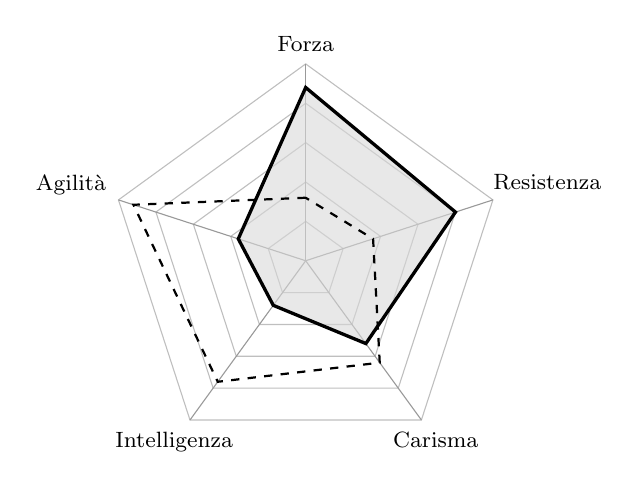
\begin{tikzpicture}[font=\footnotesize]
  \def\n{5}
  \foreach \r in {0.5,1,1.5,2,2.5} {
    \draw[black!25] (90:\r)
      \foreach \i in {1,...,4} { -- (90+\i*72:\r) } -- cycle;}
  \foreach \i/\lab in {0/Forza,1/Agilità,2/Intelligenza,3/Carisma,
                       4/Resistenza} {
    \draw[black!40] (0,0) -- (90+\i*72:2.5);
    \node[anchor=270+\i*72, inner sep=3pt] at (90+\i*72:2.55) {\lab};}
  \draw[very thick, fill=black!15, fill opacity=0.6]
    (90:2.2) -- (162:0.9) -- (234:0.7) -- (306:1.3) -- (18:2.0) -- cycle;
  \draw[thick, dashed]
    (90:0.8) -- (162:2.3) -- (234:1.9) -- (306:1.6) -- (18:0.9) -- cycle;
\end{tikzpicture}
\caption{Un grafico a radar con due profili di personaggio (valori
inventati): a colpo d'occhio si vede in quali categorie qualitative ciascuno
è spiccato.}
\label{fig:radar}
\end{figure}

\subsection{Il grafico a corde}

Nel \textbf{grafico a corde} (\emph{chord diagram}) ogni corda ha
un'\textbf{entrata} e un'\textbf{uscita}, indicata dalla punta della freccia.
L'esempio della slide mostra le \textbf{migrazioni globali} nel corso del
tempo.

\paragraph{Le relazioni tra sistemi.} Questo grafico è estremamente utile
quando si parla di \textbf{relazioni tra sistemi}. Si mettono a grafico tutti
i sistemi del gioco: il \emph{weather system}, il \emph{combat system}, gli
NPC, la vita sociale, e così via. Si mostra quanto sono collegati e in che
direzione (in un senso o in entrambi), e già a livello visivo si fa vedere
quanto, per esempio, il combattimento è collegato a tutto il resto, o quanto
un sistema invece è poco impattante e interessa relativamente meno. È un
altro modo per \textbf{mostrare} graficamente, invece di dover scrivere in
maniera esagerata, le relazioni tra i sistemi.

``Di grafici ce ne sono davvero tantissimi.'' Sta al designer imparare a
scegliere, come sempre, \emph{the right tool for the right job}; ``in questo
caso, \emph{the best tool for the right job}''.

% ---------------------------------------------------------------------
\section{La campagna di Russia in un grafico}
\label{sec:minard}

\subsection{Due avvertenze}

Per mostrare fin dove ci si può spingere, il docente ripropone un grafico già
intravisto, ``fichissimo, cioè per me è fichissimo'', con due avvertenze.
\begin{enumerate}
  \item Probabilmente lo si rivedrà al \textbf{terzo anno}, e verrà rifatta la
        stessa domanda: che cosa mostra? Ma il docente ``non cede di un
        passo'' e lo mostra lo stesso al primo anno, perché ``è troppo
        bello''. Al terzo anno, ``non mentite: noi lo sappiamo''.
  \item Il grafico è legato al \textbf{design}: fa parte di quel processo di
        \textbf{semplificazione} e di resa più grafica dei documenti di cui
        si sta parlando nelle lezioni di documentazione, e tornerà quando si
        parlerà di uno specifico tipo di documento, la ``summa'', il fine
        ultimo di questo processo.
\end{enumerate}

Il grafico viene attribuito a \textbf{Edward Tufte}, ``probabilmente il padre
delle infografiche'': ha dato i principi di base, alcuni dei quali sono
golden rules della documentazione (sezione~\ref{sec:golden-rules}), e sono
presi come base per fare UX e UI.\footnote{La mappa è in realtà opera
dell'ingegnere francese \textbf{Charles Joseph Minard} (1869). È stato Tufte,
in \emph{The Visual Display of Quantitative Information} (1983), a renderla
celebre, definendola probabilmente il miglior grafico statistico mai
disegnato.} Il docente darà poi il link a un talk che ne parla, ``uno dei
talk più belli che siano mai stati fatti sul design in generale, sul game
design in generale. A me ha aperto la mente.''

\subsection{Che cosa mostra?}

La regola del gioco: niente ``furia'', non si va a cercare che cos'è. Più ci
si spreme le meningi, più ritorno si avrà dopo. Si sa solo che è una
\textbf{variante del diagramma di Sankey}. E bisogna leggere il grafico, non i
testi (``sennò è troppo semplice'').

\begin{description}
  \item[Valerio] Potrebbe mostrare \textbf{scelte narrative} che proseguono
        con la storia. ``In questo caso no. Però è interessante: c'è un
        certo tipo di \textbf{progressione} in questo grafico.'' E, ammette il
        docente, ``ho mentito: sono due grafici'', uno sopra e uno sotto, che
        si legano tra loro.
  \item[Lorenzo] Sembra esserci una \textbf{correlazione} tra i due. La
        banda color ocra all'inizio è il 100\%; poi una parte si stacca, e
        nel tempo, procedendo, la quantità cambia, forse in un tempo comune
        alle due curve rappresentato da quella sotto. Nella banda nera si
        discrimina un'altra popolazione che si prende un'altra fetta. E
        quindi non sono percentuali ma \textbf{quantità}, perché nel tempo
        entrambe \textbf{diminuiscono}. ``Questo te lo confermo.'' Sembra uno
        strumento per analizzare più categorie e quantità correlate nel
        tempo. Il docente conferma la direzione: c'è una progressione,
        ``tra l'altro fisica''; la banda si rompe in quella nera, le
        quantità di entrambe diminuiscono, e c'è la correlazione con il
        grafico sotto, che è un \textbf{grafico a linea delle temperature}.
        Dalla classe si nota anche che la banda nera sembra ingrossarsi a
        spese dell'altra, e qualcuno azzarda un'ipotesi: petrolio bruciato e
        anidride carbonica emessa.
\end{description}

Il docente indica allora alcune linee sottili, ``con una forma che
sicuramente in vita vostra avete già visto''. Curve di livello? ``No, sono
troppo irregolari.'' Confini geografici? Una mappa delle temperature locali in
2D? Nessuno azzarda: sono \textbf{fiumi}.

\subsection{La risposta}

Il grafico mostra la quantità di uomini nell'\textbf{esercito di Napoleone
durante la campagna di Russia}, verso Mosca.
\begin{itemize}
  \item La banda chiara è la \textbf{marcia di andata}, quella nera la
        \textbf{ritirata}.
  \item La \textbf{larghezza} della banda è la grandezza dell'esercito.
  \item Durante la marcia alcuni se ne vanno: l'esercito si divide, alcuni
        tornano indietro, altri vanno avanti.
  \item In corrispondenza di un fiume si vede la banda assottigliarsi
        drasticamente: lì sono morti moltissimi uomini (``adesso io ci
        rido, ma non fa ridere'').
  \item Tutto in relazione alla \textbf{temperatura} in quei punti, che è il
        secondo grafico, sotto.
\end{itemize}

Per il docente ``è una figata'' perché, una volta letta la legenda,
\textbf{comunica immediatamente}, con un impatto grafico fortissimo, dove è
andato quell'esercito, che cosa ha vissuto, come si è piano piano non solo
separato ma anche \textbf{decimato} nel tempo: una campagna completamente
disastrosa. ``Con i grafici potete fare questa roba qua.''

\subsection{Dalle infografiche ai documenti}

In futuro si vedrà che lo stesso si può fare anche con la documentazione,
benché con i documenti di design sia veramente difficile: nella sua massima
espressione, \textbf{compressi in una singola pagina}. È il motivo per cui
Tufte è stato preso ad esempio e riadattato all'arte del documentare da
\textbf{Stone Librande}, il designer di \emph{Spore}, dei \emph{Sims} e di
altri titoli.\footnote{Nella trascrizione compare come ``Stanley Brandi''.
Il talk a cui il docente si riferisce è quasi certamente \emph{One-Page
Designs} di Stone Librande (GDC 2010), in cui la mappa di Minard e i principi
di Tufte sono il punto di partenza per i documenti di design di una sola
pagina.} Se ne riparlerà nella lezione di documentazione apposita. Non bisogna
raggiungere subito quel livello, ``perché è molto difficile, e non credo
nemmeno di esserci arrivato io''; ma il margine è tanto: \textbf{il tetto è
molto alto}. Si ragiona, si sperimenta, e si migliora nel tempo.

\paragraph{Approfondimento: Tufte nelle bibliografie di game design.} Tufte
compare nelle letture consigliate di entrambi i manuali del progetto.
Schell, in \emph{The Art of Game Design}, definisce \emph{The Visual Display of
Quantitative Information} ``la Bibbia (o almeno l'Antico Testamento) del
design delle interfacce grafiche'', e apre la sua lente della trasparenza
(\#62) con una citazione di Tufte: ``Per quanto bella sia la tua
interfaccia, sarebbe meglio se ce ne fosse di meno''. Brathwaite e Schreiber,
in \emph{Challenges for Game Designers}, consigliano \emph{Visual
Explanations}: per quanto si aderisca alle convenzioni di genere, sembra che
esistano solo uno o due modi di mostrare una barra della vita o il conteggio
delle munizioni; Tufte ``distrugge questa illusione'', mostrando molti modi
diversi di visualizzare un'informazione importante, con pregi e difetti di
ciascuno. È lo stesso messaggio della lezione: per ogni dato esiste un
grafico migliore degli altri, e trovarlo è parte del lavoro.

% ---------------------------------------------------------------------
\section{Principi per grafici migliori}
\label{sec:principi-grafici}

Ci sono comunque dei principi per migliorare, formattare e rendere più
visibili i dati di un grafico: le classiche regole della \textbf{Gestalt} e i
principi di design in generale. Cose che probabilmente si sanno già, ma è utile
ricordarle, e che si sono già cominciate ad applicare nella documentazione;
nei grafici le si può spingere ``all'esponenziale'', perché fare grafici è
``una pratica grafica, appunto''.
\begin{description}
  \item[Spazio negativo] Va sfruttato.
  \item[Scala] Ciò che è più grande impatta di più il lettore e viene
        percepito come più importante; ciò che è più piccolo, meno.
  \item[Gerarchia] L'ordine visivo delle informazioni.
  \item[Prossimità, forma, colore] Elementi vicini, della stessa forma o
        dello stesso colore vengono letti come un gruppo.
\end{description}

Al netto della ricerca (scoprire nuovi tipi di grafico, capire qual è il più
adatto) questa abilità si costruisce con l'\textbf{esperienza}: più grafici si
fanno, più si diventa abili, ``ancora di più rispetto alla documentazione
base, anche perché questo è documento''.

% ---------------------------------------------------------------------
\section{La matematica di base}
\label{sec:matematica-base}

\subsection{Quattro cose, da quinta elementare}

Non c'è tempo per un'altra pausa (``al massimo finiamo cinque minuti prima,
cosa che non è mai successa''), quindi si passa ai \emph{basic math
principles}. ``Qua siamo probabilmente in quinta elementare'': per chi non lo
sapesse non è un problema; le cose sono veramente quattro.

\subsection{La media}

La \textbf{media} (aritmetica) è la somma di tutti i numeri divisa per il
numero di elementi dell'insieme:
\[
  \bar{x} = \frac{x_1 + x_2 + \dots + x_n}{n} = \frac{1}{n}\sum_{i=1}^{n} x_i .
\]
``Su questo penso che nessuno abbia dei dubbi.''

\subsection{La media pesata}

Serve per alcuni framework o per alcuni calcoli in generale. Ci sono
\textbf{due modi} per farla.

\paragraph{Primo modo: pesi che sommano a uno.} Tutti i pesi sommati devono
dare \textbf{uno}, cioè il totale, il 100\%. Dati questi pesi, si
\textbf{moltiplica} ciascun valore per il rispettivo peso, ottenendo il valore
pesato, e poi si \textbf{somma}:
\[
  \bar{x}_w = \sum_{i=1}^{n} w_i\, x_i \qquad \text{con} \qquad
  \sum_{i=1}^{n} w_i = 1 .
\]

\paragraph{Secondo modo: pesi qualsiasi.} I pesi possono \textbf{non} dare il
100\%. Si moltiplica ciascun valore per il suo peso specifico, si sommano i
risultati, e la somma si divide per la \textbf{somma dei pesi}:
\[
  \bar{x}_w = \frac{\sum_{i=1}^{n} w_i\, x_i}{\sum_{i=1}^{n} w_i} .
\]
``Non è complessa, forse un passaggio in più.'' Il primo modo è un caso
particolare del secondo: se i pesi sommano a uno, il denominatore vale 1.

\paragraph{Un esempio.} Si vogliano confrontare due idee uscite dal
brainstorming dando un voto da 1 a 10 a tre criteri, con pesi diversi:
impatto (peso 3), costo contenuto (peso 2), coerenza con la visione
(peso 1). Un'idea con voti 8, 4 e 9 ha media semplice $(8+4+9)/3 = 7$, ma
media pesata
\[
  \frac{3\cdot 8 + 2\cdot 4 + 1\cdot 9}{3+2+1} = \frac{41}{6} \approx 6{,}83 .
\]
Con i pesi normalizzati ($3/6 = 0{,}5$; $2/6 \approx 0{,}33$;
$1/6 \approx 0{,}17$, che sommano a 1) si ottiene lo stesso risultato con il
primo modo. (L'esempio non è della lezione.)

\paragraph{Approfondimento: il valore atteso.} Schell (\emph{The Art of Game
Design}, capitolo~12) mostra uno degli usi più frequenti della media pesata
nel game design: il \textbf{valore atteso}, cioè la media di tutti i
risultati possibili di un'azione, pesati con la loro probabilità (pesi che,
come nel primo modo, sommano a uno). Se finendo su una casella verde si tira
un dado a sei facce e si ottengono altrettanti punti, il valore atteso è
$(1+2+3+4+5+6)/6 = 3{,}5$: è utile sapere che ogni volta, in media, si
guadagnano 3,5 punti. Con esiti non equiprobabili si pesa: tirando due dadi,
si vincono 5 dollari con un 7 o un 11 e se ne perde uno con qualsiasi altro
risultato. Le probabilità sono $6/36$ per il 7, $2/36$ per l'11 e $28/36$ per
il resto, quindi
\[
  \tfrac{6}{36}\cdot 5 + \tfrac{2}{36}\cdot 5 + \tfrac{28}{36}\cdot(-1)
  \approx 0{,}83 + 0{,}28 - 0{,}78 = 0{,}33 :
\]
alla lunga si vincono in media 33 centesimi a partita. Se vince solo il 7, il
valore atteso scende a zero (un gioco equo); se vince solo l'11, diventa
negativo ($-0{,}86$ circa). Schell ne fa una lente (\#35, \emph{The Lens of
Expected Value}): bilanciare un gioco passa spesso da conti di questo tipo.

\subsection{Le proporzioni}

L'ultima cosa è la \textbf{proporzione}: $a$ sta a $b$ come $c$ sta a $d$,
\[
  a : b = c : d ,
\]
dove $a$ e $d$ sono gli \textbf{estremi} e $b$ e $c$ i \textbf{medi}. La
proprietà fondamentale è che il prodotto dei medi è uguale al prodotto degli
estremi ($b \cdot c = a \cdot d$). Quindi:
\begin{description}
  \item[Incognita in un estremo] Si \textbf{moltiplicano i medi} e si divide
        per l'\textbf{estremo noto}. Esempio della lezione: in
        $100 : 35 = 20 : x$, i medi sono 35 e 20, l'estremo noto è 100:
        \[ x = \frac{35 \cdot 20}{100} = \frac{700}{100} = 7 . \]
        Verifica: 100 sta a 35 come 20 sta a 7.
  \item[Incognita in un medio] Si \textbf{moltiplicano gli estremi} e si
        divide per il \textbf{medio noto}. Esercizio della lezione: in
        $100 : 35 = x : 5$, gli estremi sono 100 e 5, il medio noto è 35. La
        classe risponde con il calcolo, ``500'', diviso 35:
        \[ x = \frac{100 \cdot 5}{35} = \frac{500}{35} \approx 14{,}3 , \]
        che il docente arrotonda a 14: 100 sta a 35 come (circa) 14 sta
        a 5.
\end{description}

``Avete tutte le informazioni basilari di matematica per sopravvivere alla
quinta elementare e al primo anno.''

\subsection{Che cosa verrà dopo}

Il discorso si complicherà al secondo anno, quando si parlerà di
\textbf{regressione lineare}: ma sono strumenti che servono per framework
specifici o per lavori specifici. Fare l'\textbf{economy designer} li
richiede, e anche un \textbf{data analyst} ha determinate competenze
matematiche; li si tratterà lì, punto per punto. Per ora interessa solo che
si ricordino queste quattro cose: semplici, ma ``una rinfrescata e averle lì
non vi fa male''.

% ---------------------------------------------------------------------
\section{Chiusura e prossimi appuntamenti}
\label{sec:chiusura-gd6}

La lezione è finita (``yes, abbiamo finito''), con un leggero margine di
anticipo. Il docente ricorda le scadenze:
\begin{itemize}
  \item il \textbf{production dictionary} per \textbf{lunedì 2}
        (sezione~\ref{sec:task-gd4});
  \item il \textbf{flowchart di Pac-Man} (o di \emph{Donkey Kong}) per
        \textbf{venerdì 6} (sezione~\ref{sec:task-gd6});
  \item l'altro task è già stato consegnato: il docente lo commenterà nel
        fine settimana o, al massimo, all'inizio della settimana successiva.
\end{itemize}

\paragraph{Leggere i commenti prima del 6.} Dopo che il docente avrà
commentato, bisogna \textbf{leggere i suoi commenti prima della lezione del
6}: in quella lezione si prenderà una pagina bianca e si comincerà a
documentare e a formattare la pagina insieme (sezione~\ref{sec:recap-documentazione}),
e prima di farlo è importante che il feedback ricevuto sia stato compreso.
Come detto l'altra volta, bisogna aspettare che il docente abbia commentato
tutto.

``Per lunedì portate il PC, perché Alessandro ne sarà sicuramente contento.''
I saluti sono di stagione: ``Buon Halloween! Buona festa dei morti!''

% ---------------------------------------------------------------------
\section*{Punti chiave del capitolo}
\addcontentsline{toc}{section}{Punti chiave del capitolo}

\begin{itemize}
  \item Nel \textbf{production dictionary} vanno i \textbf{nomi} unici o
        fraintendibili del gioco, spiegati in una o due righe (che cos'è una
        MT, che cos'è un tipo); il funzionamento profondo va nei documenti
        dedicati. Ordine alfabetico per leggibilità, ma le voci legate tra
        loro possono stare vicine; in ogni caso, \textbf{ordinato}.
  \item Nel brainstorming \textbf{nessuno viene fermato}, tutti parlano, si
        elenca tutto, si cercano background diversi. Un
        \textbf{facilitatore} (non un leader) fa sentire tutti ascoltati e
        tiene il brainstorming su uno scopo pratico. \textbf{Pause} e
        \textbf{cibo} riducono la tensione.
  \item Altre tecniche: circle, acting brainstorming, i \textbf{sei
        cappelli} di de Bono (partire dal verde; il nero è già giudizio),
        l'oggetto dal cappello, storyboard, domande, ``peggiore è, meglio
        è'', associative e \textbf{mind mapping}, il \textbf{TRIZ} (matrice
        di parametri, soluzione già nella cella, adatto a problemi
        fisici).
  \item Le regole di \textbf{Kawasaki} (make meaning, make mantra, next
        curve, DICEE, don't worry be crappy, hundred flowers, polarize,
        churn, niche, perfect your pitch) e lo \textbf{SCAMPER}. Il pitch si
        prova e riprova, ma \textbf{non si impara a memoria}.
  \item Dalle cento idee ad \textbf{almeno dieci}: \textbf{brainstorming
        matrix} impatto/effort, confronto, compromesso; contano anche la
        \textbf{motivazione} del team e la visione. Le idee vanno
        \textbf{distrutte}: se non si trova nessun difetto, c'è un problema.
  \item \textbf{KISS}: prototipare subito il cuore del gioco; muoversi,
        cambiare prospettiva, \textbf{rituali} che rompono la routine (il
        playtest del venerdì).
  \item Il \textbf{flowchart} è una rappresentazione grafica formalizzata di
        un processo; nasce nel software, e ai designer serve per IA,
        pipeline, game loop, sequenze di gameplay, player journey, UI.
        Serve a \textbf{mostrare invece di scrivere}.
  \item Regole: si legge \textbf{dall'alto in basso e da sinistra a
        destra}, nella direzione delle frecce; stesso livello, stessa
        gerarchia; il layout orizzontale evita il \textbf{wall of text}.
  \item Blocchi: \textbf{inizio/fine} (rettangolo arrotondato, obbligatori),
        \textbf{azione} (rettangolo), \textbf{decisione} (rombo, uscite
        sempre etichettate), \textbf{sotto-processo} (da spiegare in un altro
        flowchart), \textbf{input/output} (parallelogramma),
        \textbf{documento}.
  \item In un sistema o un loop di gioco il flusso \textbf{deve chiudersi o
        tornare indietro}: nessun ramo nel nulla. Le regole prima si
        imparano, poi si piegano (Oxenfree, il gioco di carte, Machinations,
        il behavior tree).
  \item Task: il \textbf{flowchart completo di Pac-Man} (Daniele:
        \emph{Donkey Kong}), come immagine leggibile e commentabile,
        esportata al 300--500\%, per venerdì 6.
  \item Grafici: \textbf{linea} per l'evoluzione continua e le previsioni,
        \textbf{gradini} per i salti discreti e le progressioni; barre e
        colonne (con legenda prima), istogrammi, torta e ciambella, aree,
        clustering; poi treemap, sunburst, \textbf{radar}, \textbf{corde}
        (relazioni tra sistemi) e la mappa di Minard resa celebre da Tufte.
        Il tetto è altissimo: fino ai documenti di una pagina di Librande.
  \item Matematica di base: \textbf{media}, \textbf{media pesata} (pesi che
        sommano a uno, oppure divisione per la somma dei pesi; il valore
        atteso ne è un caso), \textbf{proporzioni} (medi per medi, estremi
        per estremi).
\end{itemize}

%    \part{Laboratorio: le revisioni dei task}
%    \renewcommand{\thechapter}{R}
%    \renewcommand{\theHchapter}{R}   % solo con hyperref
%    % =====================================================================
%  Capitolo R — Gli errori nei task: revisioni, correzioni e consigli
%  del docente (capitolo "vivo", da aggiornare a ogni revisione)
%  Fonte: i documenti dei task consegnati dalla classe, con i commenti
%  di revisione di Mattia Podini (Google Docs esportati in .docx).
%  Task coperti finora:
%    T1  Arcade core elements  (revisioni del 28/10/2026, 9 documenti
%        di 8 studenti, circa 350 commenti)
%    T2  Production dictionary di un Pokémon (revisioni del 5-6/11/2026,
%        9 documenti di 9 studenti, 173 commenti del docente e 3 risposte
%        di studenti; .docx in tasks/revisionati/
%        2026-11-05_PokemonProductionDictionary/)
%    T3  TCG pain points, a gruppi (revisioni del 7/11/2026, 4 documenti
%        di 4 gruppi, 80 commenti; .docx in tasks/revisionati/
%        2026-11-07_TCGPainPoints/)
%    T4  Flowchart di Pac-Man (revisioni dell'11/11/2026, 8 consegne,
%        79 commenti: immagini commentate su Drive, PDF annotati e due
%        .docx; il task di Lorenzo in tasks/gd6-pacman-flowchart/)
%    T5  Compendium e High Vision di Metroid Dread (revisioni del
%        18/11/2026, 14 documenti di 7 studenti, 235 commenti; .docx in
%        2026_11_13_MDCompendium&HighVision/)
%    T6  Feedback ai concept art di Zoe, gioco di zombie (revisioni del
%        19/11/2026, 7 documenti, 113 commenti; il task di Lorenzo in
%        tasks/gd10-zombie-feedback/)
%
%  Pacchetti richiesti nel preambolo del libro: gli stessi di GD6
%    \usepackage[italian]{babel}, \usepackage[T1]{fontenc},
%    \usepackage[utf8]{inputenc} (solo pdfLaTeX), \usepackage{booktabs},
%    \usepackage{tikz} con le librerie di GD6 (qui servono
%    arrows.meta, positioning, calc). Nessun pacchetto nuovo.
%
%  Collocazione nel libro: una parte propria, in coda al corso, con
%  numerazione "R" (Revisioni):
%
%    \part{Il corso di Game Design}
%    ...
%    % =====================================================================
%  Capitolo 6 — Dal brainstorming ai flowchart: come si conduce un
%  brainstorming, flowchart, grafici e matematica di base
%  (problema e soluzione, terza e ultima parte; documentazione visiva)
%  Fonte: trascrizione della lezione GD6 (Game Design, primo anno)
%  Pacchetti richiesti nel preambolo del libro:
%    \usepackage[italian]{babel}, \usepackage[T1]{fontenc},
%    \usepackage[utf8]{inputenc} (solo pdfLaTeX), \usepackage{booktabs},
%    \usepackage{amsmath}, e in più, novità di questo capitolo:
%    \usepackage{tikz} con
%    \usetikzlibrary{shapes.geometric,shapes.symbols,shapes.misc,
%      arrows.meta,positioning,calc,fit}
%    (le librerie vanno caricate nel preambolo, non nel capitolo)
%  Nota sulla fonte: la trascrizione automatica storpia diversi nomi
%  propri (titoli, strumenti, autori) e contiene lunghi tratti ripetuti
%  in loop durante le due pause. Dove il riferimento è ricostruibile con
%  certezza lo si riporta nella forma corretta; dove non lo è, lo si
%  segnala in nota invece di indovinare. Le figure sono ricostruzioni
%  degli esempi mostrati a lezione (slide e lavagna draw.io), non copie.
% =====================================================================

\chapter[Dal brainstorming ai flowchart]{Dal brainstorming ai flowchart:
condurre un brainstorming, flowchart, grafici e matematica di base}
\label{cap:brainstorming-flowchart}

Con questo sesto capitolo si chiude, finalmente, la lunga lezione su
\emph{problema e soluzione} cominciata due capitoli fa
(capitolo~\ref{cap:problema-soluzione}) e proseguita nel precedente
(capitolo~\ref{cap:ricerca-idee}). Mancava l'ultima parte: \emph{come} si
conduce un brainstorming, con quali regole, quali tecniche e come si passa
da cento idee a una manciata di idee valutate. Chiusa quella, la giornata
cambia argomento e apre un blocco nuovo, dedicato agli strumenti
\textbf{visivi} della documentazione: i \textbf{flowchart}, i
\textbf{grafici} e quel poco di \textbf{matematica di base} che serve per
costruirli e leggerli.

La lezione, un venerdì pomeriggio a ridosso di Halloween, si tiene da remoto
ed è condotta ancora da Mattia Podini. Il percorso del capitolo ne ricalca la
struttura:
\begin{enumerate}
  \item le domande in apertura, ancora una volta sul \textbf{production
        dictionary} di Pokémon: che cosa si intende per
        \emph{nomenclatura}, come ordinare le voci, che cosa lasciare ad
        altri documenti (sezione~\ref{sec:pd-gd6});
  \item la conclusione della parte sul \textbf{brainstorming}: le condizioni
        per farlo bene, il \textbf{facilitatore}, le pause e il cibo
        (sezioni~\ref{sec:ripresa-gd6} e~\ref{sec:condurre-brainstorming});
  \item altre \textbf{tecniche} per generare idee, dai \emph{sei cappelli} al
        \textbf{TRIZ}, le regole dell'innovazione di \textbf{Guy Kawasaki} e lo
        \textbf{SCAMPER} (sezioni~\ref{sec:altre-tecniche}
        e~\ref{sec:kawasaki-scamper});
  \item come si passa \textbf{dalle cento alle dieci idee}: la
        \emph{brainstorming matrix}, il confronto, il tentativo di
        distruggere le proprie idee, il prototipo e le routine da spezzare
        (sezioni~\ref{sec:sortare-idee} e~\ref{sec:kiss-routine});
  \item i \textbf{flowchart}: che cosa sono, dove nascono, a che cosa servono
        a un designer, le regole di lettura, i blocchi, l'obbligo di chiudere
        il flusso, e una serie di esempi reali che le regole le piegano
        (sezioni~\ref{sec:flowchart-cosa}--\ref{sec:flowchart-esempi});
  \item il task della settimana: il \textbf{flowchart completo di Pac-Man}
        (sezione~\ref{sec:task-gd6});
  \item i \textbf{grafici}: un piccolo esercizio in aula (linea o gradini?),
        i grafici di base, quelli più ricchi e la mappa della campagna di
        Russia di Napoleone, ``uno dei grafici più belli mai fatti''
        (sezioni~\ref{sec:grafici-esercizio}--\ref{sec:principi-grafici});
  \item la \textbf{matematica di base}: media, media pesata, proporzioni
        (sezione~\ref{sec:matematica-base}).
\end{enumerate}

% ---------------------------------------------------------------------
\section{In apertura: ancora il production dictionary}
\label{sec:pd-gd6}

\subsection{Prima di cominciare}

L'avvio è il solito avvio di una lezione online: il docente non sente la
classe (``probabilmente perché non ho ancora condiviso lo schermo''), segna le
presenze, saluta chi entra. Poi il rituale: domande o dubbi sulla lezione
precedente, che oggi si conclude, o sui task in generale, ``anche perché il
production dictionary scade lunedì'' (il task del
capitolo~\ref{cap:problema-soluzione}, sezione~\ref{sec:task-gd4}).

\paragraph{Problemi di gameplay, prima di tutto.} La prima domanda riguarda
invece il task a gruppi sui \emph{pain point}
(sezione~\ref{sec:task-gd5}): i tre problemi principali trovati devono
riguardare il gameplay o possono toccare qualsiasi feature del gioco, per
esempio il negozio? Qualsiasi tipo di feature, chiaramente. Il docente però
\textbf{sconsiglia} di prendere un problema \textbf{artistico} o un problema
di \textbf{performance}: se davvero non si trova altro, lo si può includere
come punto finale, ma la priorità va ai \textbf{problemi di gameplay}.

\subsection{Che cosa si intende per nomenclatura}

Mattia, uno studente, confessa di non aver ancora capito la consegna del
production dictionary. Ha provato a lavorarci in una cartella personale, ma
si è accorto che stava scrivendo e \emph{spiegando meccaniche}, e ha il
sospetto che non sia quello che viene chiesto. ``Che cosa si intende per
nomenclatura?''

Il docente ricorda di averlo già ripreso all'inizio della lezione precedente
(sezione~\ref{sec:pd-ripreso}) e lo rispiega. L'obiettivo è spiegare
\textbf{nomi unici legati al gioco}, o alla produzione del gioco. Possono
essere nomi di meccaniche, e nel caso di Pokémon lo possono essere
tranquillamente; ma più spesso sono nomi che spiegano un oggetto del mondo,
un \emph{game object} del mondo di Pokémon. L'esempio è il \textbf{tipo} (o
elemento): si spiega che cosa sono i vari tipi, che cos'è il tipo di un
Pokémon.

\paragraph{Che cosa \emph{non} ci va.} Negli esempi mostrati nelle slide,
come la voce \emph{Chase} (lo stato di inseguimento di un'intelligenza
artificiale, sezione~\ref{sec:production-dictionary}), è chiaro che quello
stato non verrà spiegato in un documento dedicato solo a lui: sarà spiegato
nel documento delle IA. Lì si trovano le spiegazioni \textbf{profonde}: come
funziona la meccanica, che parametri ha, che cosa richiede lato
programmazione, lato arte e così via. Nel production dictionary finisce
invece \textbf{a che cosa è legato quel nome}, a livello descrittivo: una o
due righe, una descrizione succinta. Lo scopo è che il lettore, di qualunque
natura sia (artista, grafico, programmatore, designer), sappia \textbf{a che
cosa si riferisce quella parola}.

\paragraph{La webcam, per favore.} A metà spiegazione il docente chiede a
Mattia di accendere la webcam: ``già faccio fatica a leggere naturalmente i
volti delle persone, figuriamoci se non ti vedo''; vuole capire se la
spiegazione arriva o no. Il problema dello studente era proprio questo:
quando si metteva a scrivere, gli veniva spontaneo descrivere le meccaniche,
non le nomenclature.

\subsection{Priorità: un limite di una pagina}

Per tutto ciò che è estremamente specifico si fa riferimento ai
\textbf{singoli documenti}. E gli studenti hanno anche il limite di
\textbf{una pagina}, quindi devono per forza scegliere le nomenclature
\textbf{più importanti} del gioco. Con molto più spazio si potrebbe discutere
se spiegare meccaniche uniche, specifiche, o qualcosa di estremamente
laterale.

\paragraph{Un caso limite.} Spiegare una singola mossa molto particolare è un
caso estremamente unico,\footnote{Nella trascrizione la mossa compare come
``fuoco-bomba''; non è chiaro a quale mossa o meccanica ci si riferisca.
L'esempio vale comunque come caso estremamente specifico.} ben diverso dallo
spiegare, per esempio, che cos'è una \textbf{MT} o una \textbf{MN}. E anche
per le MT conviene separare due piani:
\begin{itemize}
  \item \textbf{come funziona il sistema}: se una MT è consumabile o no,
        quante mosse ci sono e così via; questo può essere relegato ad altra
        documentazione;
  \item \textbf{che cos'è}: questo sì, è materia da dizionario.
\end{itemize}
Ancora più a monte si potrebbe spiegare che cos'è un \emph{oggetto} di gioco,
un item della borsa; ma ``oggetto'' è abbastanza comprensibile. L'ultima
parola spetta agli studenti, ma il criterio del docente è questo: si parla di
\textbf{nature uniche del gioco}, oppure \textbf{fraintendibili}. È questa
l'utilità del documento.

\paragraph{Non è un errore, è un'altra scelta.} Quello che allo studente
veniva istintivamente da fare non è sbagliato di per sé: rispetto alla
consegna è un'altra cosa, ma dal punto di vista della produzione non è un
errore. Come detto l'ultima volta, il production dictionary si può
\textbf{ibridare} con altri documenti (sezione~\ref{sec:pd-ripreso}): lo si
può mettere all'inizio di un documento, oppure spiegare le singole
terminologie in un GDD o in un altro tipo di documentazione, e allora quello
è il documento che spiega quella meccanica. Se il gioco \textbf{non ha un
grande rischio di fraintendimento}, si può anche valutare di avere un
documento a sé che funge da dizionario: non è obbligatorio.

\subsection{Raggruppare o ordinare alfabeticamente?}

Intanto Lorenzo ha la webcam spenta: ``vedo che Lorenzo si è affondato
nell'erba alta ed è diventato un Pokémon''. La parola passa a Valerio, che
ha stilato una serie di elementi e, siccome erano tanti, li ha
\textbf{raggruppati per fili comuni}. È sbagliato?

Dipende dal numero, dalla mole di informazioni che si danno al lettore. Su
una pagina sola può funzionare; quale sia la scelta ideale il docente non
può dirlo (``sennò poi dopo me la modificate''). Ma il ragionamento è
questo, esattamente come per un dizionario:
\begin{itemize}
  \item la \textbf{maggior leggibilità}, nel vuoto, ce l'ha l'\textbf{ordine
        alfabetico};
  \item l'ordine alfabetico però non risolve un problema: alcune
        nomenclature sono \textbf{legate ad altre}. L'esempio, forse un
        azzardo, è \emph{Pokémon} e \emph{Poké Ball}: al lettore potrebbe
        essere utile sapere prima l'informazione più rilevante e subito
        dopo quella associata.
\end{itemize}
Nel caso degli studenti può contare meno; in production dictionary
esageratamente grossi conta di più. In ogni caso, se il production dictionary
c'è (e non è una necessità averlo nella produzione), \textbf{deve essere
ordinato}.

\paragraph{I problemi di stato.} Valerio ha anche parlato delle lotte,
elencando e descrivendo tutti i \textbf{problemi di stato}: dovrebbero stare
in un documento a parte, dedicato alle lotte? ``Posso fare un esempio?''
``Certo che puoi farlo, però io poi sarò libero di non risponderti.'' È più
un problema di \textbf{priorità sulle nomenclature}; sul fatto di avere un
documento a parte o meno, il docente preferisce non rispondere adesso: se ne
riparlerà dopo che avrà commentato il documento.

Una piccola nota di colore chiude il giro: Mattia non sa come abbassare la
mano su Zoom. ``Non sono lo Zoom guru, quindi figurati.''

% ---------------------------------------------------------------------
\section{Dove eravamo rimasti}
\label{sec:ripresa-gd6}

\subsection{La forbice che si allarga}

Se non c'è altro, si conclude la lezione su problema, idea, ricerca e
brainstorming. L'ultima volta ci si era fermati quasi alla fine: manca
la parte sulle \textbf{metodologie per fare brainstorming}.

Il docente ricorda una cosa che vale per tutta la lezione: più si va avanti,
dall'inizio verso la fine, più \textbf{la forbice si amplia}.
\begin{description}
  \item[Nella ricerca] non ci sono limiti, ma c'è almeno una struttura: una
        forma dei dati, delle priorità (target audience, competitor e così
        via). Dare priorità è soprattutto una questione di
        \textbf{tempistiche}: in pre-produzione il tempo sarà poco e ci sarà
        tanto da fare, quindi quanto più si riesce a coprire di quella lista
        non omnicomprensiva (la mappa della ricerca,
        sezione~\ref{sec:mappa-ricerca}), meglio è. Alcune cose andrebbero
        fatte subito: i \textbf{competitor}, fondamentali, e
        l'\textbf{utente}, più di tutti; anche il \textbf{mercato} è
        importante. Le priorità ci saranno per forza, perché il tempo non è
        infinito. E per la ricerca strutture e framework ce ne sono, e sono
        abbastanza codificati: la lista vista (le Liberating Structures),
        la SWOT analysis, la perceptual mapping
        (sezione~\ref{sec:perceptual-mapping}).\footnote{Nella trascrizione
        compaiono come ``la lista di pesciola'' (verosimilmente un
        riferimento storpiato alla lista delle Liberating Structures,
        sezione~\ref{sec:problema-necessita}) e ``swap analysis'', che è
        quasi certamente la SWOT analysis (\emph{Strengths, Weaknesses,
        Opportunities, Threats}).}
  \item[Nell'ideazione] e nel brainstorming le tecniche ci sono, ma il campo
        è \textbf{probabilmente infinito}. Si può adottare più o meno
        quello che si vuole, soprattutto a seconda del gruppo che fa
        brainstorming: non è detto che ci sia l'intero team, magari solo il
        team di design, o un \emph{feature team} all'interno del team di
        design. A seconda di chi si è nel team e di quanto è grande, si può
        davvero fare quello che si vuole: ``potete giocare a freccette,
        far venire in mente le idee, o giocare a biliardo, davvero
        qualsiasi cosa funziona''.
\end{description}
Va bene tutto, \textbf{fintanto che porta un risultato}: quella
``fantomatica'' ideazione di \textbf{cento idee} da \emph{sortare} e scartare
(sezione~\ref{sec:principi-brainstorming}).

% ---------------------------------------------------------------------
\section{Come si conduce un brainstorming}
\label{sec:condurre-brainstorming}

\subsection{Le condizioni}

Ci sono però alcune condizioni importanti.

\paragraph{Nessuno viene fermato.} Durante il brainstorming, cioè nel momento
in cui si generano le idee, \textbf{nessuno deve essere fermato} dal
generarle. Non si scartano subito potenziali idee che ``non c'entrano
nulla'': \textbf{le si elenca tutte}. Poi, eventualmente, ci sarà una fase,
insieme o da soli, in cui queste idee vengono \textbf{filtrate}.

\paragraph{Tutti devono poter parlare.} Tutti devono sentirsi nella
condizione di dire la propria e di far crescere quella grande lista di idee,
che alla fine dei conti è l'obiettivo: buttare giù davvero qualsiasi cosa.
Anche perché quello che verrà scartato può ritornare in un'altra forma, in
un'altra maniera, o anche solo far scaturire qualche idea nuova per
implementazioni future. Qualsiasi spunto è utile: lasciare la parola a
tutti, e nella fase di brainstorming \textbf{qualsiasi cosa va bene}.

\paragraph{Non solo designer.} Sempre per arrivare a una quantità maggiore,
e potenzialmente più \textbf{diversificata}, di idee, conviene avere nel
brainstorming \textbf{non solo designer}, o comunque non solo persone con lo
stesso background. A seconda di quanto sono disponibili e di quanto sono
dentro l'industria, si cercano \textbf{punti di vista diversi}: l'obiettivo è
ampliare la propria visione il più possibile.

\subsection{Il facilitatore}

Questo vale sicuramente per i team grossi, ma va valutato anche per quelli
piccoli, soprattutto le prime volte, se c'è difficoltà a parlare o se si è
meno portati a rompere il ghiaccio o a essere espansivi: conviene avere un
\textbf{facilitatore}. Non un leader, ma qualcuno che si preoccupa di
\textbf{controllare il flusso} del brainstorming: quanto tempo si sta
spendendo a discutere di un'idea, o ``a tirare quella freccetta''.

Il facilitatore ha fondamentalmente \textbf{due obiettivi}:
\begin{enumerate}
  \item \textbf{assicurarsi che tutti stiano bene} durante il brainstorming.
        A livello pratico vuol dire che tutti parlino e abbiano lo stesso
        tempo per parlare; ma c'è un passo in più, che tutti si sentano
        \textbf{a proprio agio}. Garantire la parola a tutti non basta
        necessariamente: a seconda dei membri del team, e di quanto li si
        conosce, l'obiettivo è \textbf{farli sentire ascoltati};
  \item \textbf{assicurarsi che il brainstorming abbia uno scopo pratico}.
        Fare brainstorming ``è una figata, piace a tutti'', ma il rischio
        di ``buttarla in caciara'' è molto grosso. È bello avere un momento
        di comunione con il team, più o meno regolamentato; tuttavia
        \textbf{bisogna quagliare}, arrivare a una lista lunga e concreta di
        idee. Il facilitatore si chiede quanto tempo va dedicato al
        brainstorming (un'ora?), controlla che si stia andando nella
        direzione corretta ed eventualmente \textbf{tira le redini} se
        qualcuno sta divagando.
\end{enumerate}

\paragraph{Approfondimento: chi deraglia, rimette sui binari.} Schell, tra i
suoi sedici consigli pratici per il brainstorming (\emph{The Art of Game
Design}, capitolo~7), incoraggia a \textbf{fare battute}: le battute
sciolgono la mente e fanno vedere le cose da prospettive che si erano perse,
ed è dalle prospettive nuove che nascono le grandi idee. Ma avverte che,
soprattutto in gruppo, le battute possono portare fuori strada; uscire dai
binari ogni tanto va bene (``le idee buone potrebbero non essere sui
binari''), purché ci si prenda la responsabilità di rientrarci. Il suo
comandamento è: \emph{he who derails, rerails}, chi fa deragliare rimette sui
binari. È, in piccolo, il secondo compito del facilitatore distribuito su
tutti i partecipanti.

\subsection{Pause e cibo}

\paragraph{Fare delle pause.} Conviene avere \textbf{pause tra una fase e
l'altra}. Al secondo anno si parlerà meglio di come affrontare la produzione,
di come lavorare con altri esseri umani, dell'importanza delle soft skill;
cose importanti, che il docente non vuole sminuire, ma il primo anno è il
campo di prova. Le pause servono a ridurre ``il cortisolo, mettiamola
così'': evitare che le persone impazziscano o che comincino a percepirsi
\textbf{screzi} forti tra gli individui.

È il discorso precedente visto dall'altro lato: se non si fa parlare tutti,
e soprattutto se qualcuno comincia a \textbf{smontare le idee}, o fa già la
fase di prendere un'idea e buttarla subito fuori dal cesto perché non ha
senso con i limiti, con la visione o con quello che si vuole, qualcuno
potrebbe ``inalberarsi'', prenderla male. E si ammetta pure che il team sia
grosso e che ci siano già delle inimicizie al suo interno.

\paragraph{Portate il cibo.} Per risolvere questo problema: pause, e poi
\textbf{cibo}. Lo si vedrà in modo più strutturato al secondo anno, ma il
mantra è: ``portate il cibo, portate la pizza. Non lo so, quello che
mangiano gli esseri umani generici. Io non mangio la pizza, però\dots''.
Generalmente avere delle pause in cui si mangia e si beve \textbf{aiuta
notevolmente a ridurre la tensione}.

% ---------------------------------------------------------------------
\section{Altre tecniche per generare idee}
\label{sec:altre-tecniche}

\subsection{Una lista, non un programma}

I modi per fare brainstorming, per generare idee in generale, sono tanti. Il
docente non li vede tutti punto per punto, ma li elenca; si aggiungono a
quelli già visti nel capitolo precedente (sezione~\ref{sec:tecniche-idee}).

\subsection{Circle}

Ci si mette \textbf{in cerchio}, si scrive una parola, si va avanti. Si
comincia con, per esempio, il tipo di gioco, una \emph{game quality}, un tema,
un'emozione; si passa il foglietto alla persona successiva, che aggiunge
un'altra parola, e così via finché il giro non è finito. A volte si fanno
più giri. È un modo per \textbf{ibridare la propria idea iniziale con
quelle degli altri} e vedere che cosa esce.\footnote{Il docente lo associa,
``se non sbaglio'', a un gioco dei futuristi. Il meccanismo descritto
(ciascuno aggiunge un pezzo senza controllare l'insieme) ricorda piuttosto il
\emph{cadavre exquis} dei surrealisti.}

\subsection{Acting brainstorming}

Si \textbf{mette nei panni di un'altra persona}: nella slide, una persona
famosa, un personaggio famoso. Ma vale anche, più in generale, per mettersi
nei panni di qualcun altro: avere la capacità \textbf{empatica} di vedere come
si è percepiti dall'altra parte, o che cosa si potrebbe provare dall'altra
parte.

\paragraph{Fuori dal brainstorming.} Il concetto è utile ben oltre la fase di
brainstorming. Un esempio: un 3D artist o un concept artist consegna i suoi
concept e gli vengono rimandati indietro, ogni volta, per una determinata
ragione. È ovvio, o almeno molto probabile, che il suo \textbf{morale} si
riduca. Mettersi nei suoi panni aiuta; poi bisognerà capire perché succede e
come risolverlo. Mettersi nei panni dell'altro aiuta a spiegare alcune
problematiche della produzione e del team: il morale basso, una persona che
non è mai presente o che non parla mai durante i meeting. Come sempre, si
cerca di arrivare alla \textbf{radice del problema}
(sezione~\ref{sec:problema-necessita}).

\subsection{I sei cappelli}

I \textbf{sei cappelli} vengono da un libro\footnote{\emph{Six Thinking Hats}
di Edward de Bono (1985), noto in italiano come \emph{Sei cappelli per
pensare}.} e possono essere utili per diversi tipi di attività. Ogni cappello
ha una \textbf{durata specifica} a seconda dell'attività ed è associato, un
po' come nell'acting brainstorming, alla necessità di guardare o di agire da
un determinato punto di vista:
\begin{description}
  \item[Blu] la \emph{big picture}: si guarda il problema ad alto livello;
  \item[Bianco] fatti e informazioni: si guardano i fatti, i dati;
  \item[Rosso] più istintivo: \emph{feelings and emotions};
  \item[Nero] il \textbf{giudizio critico}. Questo \textbf{rompe la fase di
        brainstorming}: è utile quando si comincia già a \emph{sortare} le
        idee, ``senza ciarle'';
  \item[Giallo] estremamente positivo: ``yes'', sorriso ``a 34 denti'', si va
        avanti;
  \item[Verde] le \textbf{idee nuove}.
\end{description}
È chiaro quindi che la fase di brainstorming dovrebbe partire col
\textbf{verde}, e comunque avere tanti momenti ``col cappello verde''. A volte
si passa da una fase all'altra; la lista completa è nel libro, che non è
necessario leggere, ma si trova anche in giro.

\subsection{L'oggetto dal cappello}

``Questo piace particolarmente a Diego'', il direttore del corso, e serve a
mostrare ancora una volta che nel generare idee si può infilare dentro
qualsiasi cosa. Si sfruttano \textbf{oggetti particolari, gadget}, pescati da
un ``fantomatico'' cappello, e si fa brainstorming su quell'oggetto: che cosa
c'entra, e come può aiutare a risolvere il problema. ``Utile? Non lo so, io
non l'ho mai usato, però sta qua.''

\paragraph{Approfondimento: i giocattoli sul tavolo.} Schell propone qualcosa
di molto simile tra i suoi consigli per il brainstorming
(\emph{The Art of Game Design}, capitolo~7, \emph{Toys}): portare al tavolo
dei giocattoli, alcuni legati al problema e altri che non c'entrano niente.
Il suo paragone sono i ristoranti pieni di oggetti strani alle pareti: non
sono decorazione, sono spunti di conversazione. I giocattoli coinvolgono la
creatività anche in modo \textbf{tattile}; e se si porta un po' di
plastilina per modellare le idee, ``sembra stupido, ma la creatività è
stupida''.

\subsection{Storyboard}

Lo \textbf{storyboard} è un po' come il \emph{drawing}
(sezione~\ref{sec:tecniche-idee}): non importa saper disegnare bene o male,
importa che sia \textbf{chiaro}, anche con gli stickman. Si disegna il
processo, una potenziale storia che spieghi l'idea, che la ``metta a terra''
nel brainstorming.

\subsection{Le domande}

\textbf{Domande}: ci si butta dentro più domande possibili, su qualsiasi
cosa. È anche un modo, più o meno serio, per iniziare quel tipo di
``sortaggio'' (``non sorteggio, sortaggio''), cioè di \textbf{valutazione}
delle idee messe a terra.

\subsection{Papà e mamma: peggiore è, meglio è}

Un'altra tecnica importante è presentata nelle slide con una metafora
familiare: da una parte il \emph{papà}, la figura particolarmente
\textbf{pragmatica}; dall'altra la parte in cui ci si butta dentro davvero
qualsiasi cosa e va bene. Anzi: \textbf{peggiore è l'idea, meglio è},
almeno teoricamente. Sempre nell'idea che \textbf{tutto può aiutare}, e che
la soluzione si può trovare partendo da qualsiasi cosa.\footnote{La
trascrizione non permette di ricostruire con certezza il nome della tecnica
nella slide. L'impostazione (cercare deliberatamente le idee peggiori) è
quella nota come \emph{worst possible idea} o \emph{reverse brainstorming}.}

\paragraph{Approfondimento: scrivere tutto, anche le idee stupide.} Schell
(\emph{The Art of Game Design}, capitolo~7, \emph{Write Everything}) cita
Linus Pauling: ``il modo migliore per avere una buona idea è avere molte
idee''. Il suo consiglio è di non aspettare l'idea brillante ma di scrivere
\textbf{tutto} ciò che è anche solo lontanamente collegato al problema, ogni
idea stupida che passa per la testa: bisogna far uscire quelle stupide prima
che comincino ad arrivare quelle buone, e a volte un'idea stupida diventa
l'ispirazione per un'idea geniale. Non ci si censura, e soprattutto in
gruppo non si censurano gli altri: ``le loro idee stupide valgono quanto le
tue''.

\subsection{Associative e mind mapping}

Con l'\textbf{associative} si parte da una parola e le si associano parole
simili. Si può usare anche un \emph{word association tool}, un'IA o
qualsiasi software che associa parole.

È molto simile al \textbf{mind mapping}, che si vede di solito: ``sicuramente
l'avrete vista da qualche parte''. Quando si parla di brainstorming, la
visione pratica è generalmente questa: una \textbf{grande mappa sulla
lavagna}, che tutti devono poter vedere. Si parte da un concetto, si
dividono i rami per \textbf{categorie}, e i rami grossi portano a rami più
piccoli, con parole o concetti sempre legati alla categoria principale
(figura~\ref{fig:mind-map}).

\begin{figure}[htbp]
\centering
\begin{tikzpicture}[
    font=\small,
    centro/.style={ellipse, draw, thick, minimum width=2.6cm,
                   minimum height=1cm, align=center},
    ramo/.style={rectangle, rounded corners=3pt, draw, align=center,
                 minimum height=0.7cm, inner sep=4pt},
    foglia/.style={align=center, inner sep=2pt, font=\footnotesize},
    every edge/.style={draw}]
  \node[centro] (c) {Gioco sul\\viaggio nel tempo};
  \node[ramo] (m) at (-4.2,1.6) {Meccaniche};
  \node[ramo] (t) at (4.2,1.6) {Tema};
  \node[ramo] (e) at (-4.2,-1.6) {Emozioni};
  \node[ramo] (p) at (4.2,-1.6) {Pubblico};
  \draw[thick] (c) -- (m); \draw[thick] (c) -- (t);
  \draw[thick] (c) -- (e); \draw[thick] (c) -- (p);
  \node[foglia] (m1) at (-6.3,2.6) {riavvolgere};
  \node[foglia] (m2) at (-6.4,1.0) {loop};
  \node[foglia] (m3) at (-3.0,2.7) {paradosso};
  \draw (m) -- (m1); \draw (m) -- (m2); \draw (m) -- (m3);
  \node[foglia] (t1) at (6.3,2.6) {orologi};
  \node[foglia] (t2) at (6.4,1.0) {rovine};
  \node[foglia] (t3) at (3.0,2.7) {nostalgia};
  \draw (t) -- (t1); \draw (t) -- (t2); \draw (t) -- (t3);
  \node[foglia] (e1) at (-6.3,-2.6) {rimpianto};
  \node[foglia] (e2) at (-6.4,-1.0) {sorpresa};
  \node[foglia] (e3) at (-3.0,-2.7) {ansia};
  \draw (e) -- (e1); \draw (e) -- (e2); \draw (e) -- (e3);
  \node[foglia] (p1) at (6.3,-2.6) {puzzle lover};
  \node[foglia] (p2) at (6.4,-1.0) {sessioni brevi};
  \node[foglia] (p3) at (3.0,-2.7) {mobile};
  \draw (p) -- (p1); \draw (p) -- (p2); \draw (p) -- (p3);
\end{tikzpicture}
\caption{Struttura tipica di una mind map: un concetto centrale, rami
principali per categoria e rami secondari sempre legati alla categoria da
cui partono. Il contenuto è un esempio inventato.}
\label{fig:mind-map}
\end{figure}

\paragraph{Che cosa usare per il task.} Per il task in corso
(sezione~\ref{sec:task-gd5}) il mind mapping funziona molto bene, ma possono
funzionare anche l'associative o il circle. Questi, i più
\textbf{immediati}, sono quelli che il docente consiglia al momento.

\paragraph{Approfondimento: lo spazio ricorda.} Due consigli di Schell
(\emph{The Art of Game Design}, capitolo~7) spiegano perché la mappa sulla
lavagna funziona. Il primo (\emph{The Writing on the Wall}): in gruppo serve
una superficie che tutti vedano contemporaneamente; Schell preferisce grandi
fogli adesivi o carta da pacchi alle pareti, che si possono riposizionare,
staccare, arrotolare e conservare, per riprendere un anno dopo il
brainstorming ``come se non si fosse mai interrotto''. Il secondo
(\emph{The Space Remembers}, espressione presa da Tom Kelley): la memoria per
le liste è scarsa, ma quella per la \textbf{posizione} delle cose intorno a
noi è ottima; appendere le idee nella stanza aiuta a ritrovarle e a vederne
le connessioni. Un terzo consiglio è più sorprendente
(\emph{Number Your Lists}): \textbf{numerare} le liste le rende più facili da
discutere (``mi piacciono dalla 3 alla 7'') e, stranamente, dà alle voci una
certa dignità, così che vengono prese più sul serio.

\subsection{TRIZ}
\label{sec:triz}

Il \textbf{TRIZ}, già accennato (sezione~\ref{sec:tecniche-idee}), viene
solo ``accennato'' anche qui, perché è estremamente complesso. Nasce
nell'\textbf{Unione Sovietica}. Il concetto è un po' quello dell'astrazione
vista nel SIT, il \emph{closed world}: il problema, per come viene
formulato, contiene già la soluzione. Anzi, \textbf{non trovare la soluzione
dipende dal fatto che il problema non è formulato correttamente}. La
soluzione è già lì; per arrivarci bisogna \textbf{astrarre il problema},
trovare \textbf{soluzioni astratte} e poi \textbf{concretizzarle}. ``Questo è
il salto.''

\paragraph{Come funziona.} Il TRIZ nasce dall'analisi di un numero enorme di
\textbf{brevetti} sovietici, in cui il comune denominatore era astrarre i
problemi e vedere come erano stati risolti. Problemi e soluzioni vengono
messi in una \textbf{matrice} con righe e colonne: sulle righe e sulle
colonne ci sono le stesse \emph{feature}, da 1 a $n$ (``sono 40, se non
sbaglio, forse sono state anche aumentate nel
tempo'').\footnote{Nella formulazione classica di Genrich Altshuller la
\emph{matrice delle contraddizioni} incrocia 39 parametri tecnici (righe:
il parametro che si vuole migliorare; colonne: quello che peggiora di
conseguenza), e ogni cella suggerisce alcuni dei \textbf{40 principi
inventivi}. Versioni successive (come la \emph{Matrix 2003}) hanno esteso i
parametri. Nella trascrizione il nome compare come ``Drizzt'', ``TRIPS'' e
``TRIZZE''.} Le feature possono essere il peso di un oggetto in movimento,
il peso di un oggetto stazionario, la lunghezza di un oggetto in movimento,
la lunghezza di uno stazionario, l'area di un oggetto in movimento, e così
via.

Se si riesce ad astrarre il proprio problema e a trovare la riga e la
colonna su cui si fonda, si va a cercare la \textbf{cella} che le combina.
Un esempio: il problema è mantenere caldo il contenuto di un bicchiere
\textbf{senza far scottare le mani} di chi lo tiene. Il calore fa parte di
quel tipo di feature: si cerca la cella che combina la colonna e la riga del
problema.

\paragraph{Piegarsi alle regole.} Il TRIZ si basa principalmente su
\textbf{problemi meccanici}, e non è facile. La soluzione, se si usa il TRIZ,
\textbf{deve derivare da quello che viene consigliato nella cella}: per
usarlo non basta conoscerlo, bisogna anche piegarsi alle sue regole. Può
essere un buon modo, se ci si leggono righe e colonne, soprattutto per
\textbf{problemi pratici di produzione fisica}: per esempio nei giochi da
tavolo, dove la stampa, la grandezza o il costo di una componente è
eccessivo. Ma resta estremamente codificato: è tra le cose che si possono
approfondire.

% ---------------------------------------------------------------------
\section{Le regole di Kawasaki e lo SCAMPER}
\label{sec:kawasaki-scamper}

\subsection{Le regole dell'innovazione di Guy Kawasaki}

Le \textbf{regole di Kawasaki} non vengono viste nel dettaglio: i punti sono
segnati nella slide, per andare veloci, e chi vuole può guardare il video,
``classico video di TEDx, informativo fino a un certo
punto''.\footnote{Guy Kawasaki, \emph{The Art of Innovation}, TEDxBerkeley,
2014. Nella trascrizione diversi titoli delle regole sono storpiati
(``Con la nice people'', ``Charm baby charm'', ``Nishita e Sensor'',
``Dot worried e crappy''); qui sono riportati nella forma originale.}
Alcune cose sono già state viste. Il docente le commenta così:
\begin{description}
  \item[Make meaning] (e non soldi). Se l'obiettivo è questo, l'obiettivo è
        portare \textbf{innovazione}; poi arriva il guadagno. Però non è
        detto: va valutato attentamente.
  \item[Make mantra] Può essere utile durante il \textbf{pitch}: servono frasi
        che catturino l'audience o che facciano capire il prodotto in poche
        parole.
  \item[Jump to the next curve] Far \textbf{evolvere} la propria idea:
        iterare, ma in positivo, sempre in modo migliorativo.
  \item[Roll the DICEE] Creare qualcosa di elegante, completo, profondo,
        intelligente, non semplice.\footnote{L'acronimo di Kawasaki è
        DICEE: \emph{deep, intelligent, complete, empowering, elegant}.} Lo si
        può paragonare al \textbf{design elegante}
        (sezione~\ref{sec:design-elegante}) che, ripete il docente, non è
        sempre necessario, ma ``è lì''.
  \item[Don't worry, be crappy] Creare \textbf{prototipi}: arrivarci il prima
        possibile e \textbf{non avere paura di fare schifo}.
  \item[Let a hundred flowers blossom] Lasciare che \textbf{nuove dinamiche}
        emergano. Applicato ai videogiochi: che emergano nuove meccaniche, o
        che i giocatori vedano e usino in modo diverso le cose che si erano
        previste. Con il \textbf{playtest} si valuta se il giocatore fa
        qualcosa a cui non si era pensato, che non si pensava possibile, e se
        ha senso all'interno della propria visione. Generalmente
        assecondare l'utente quando legge qualcosa a modo suo (ammesso che
        sia il proprio target audience) è positivo: non sempre, ma nella
        stragrande maggioranza dei casi. Il controllo del progetto resta però
        al team: è il team a decidere \textbf{se quel bug diventa una feature
        o no}.
  \item[Polarize people] Se ne riparlerà nella lezione sul feedback, ma se ne
        è già cominciato a parlare. Le persone, statisticamente, su un
        argomento si distribuiscono su una \textbf{curva a campana}.
        Interessa capire chi sono gli \textbf{estremi}: chi ama alla follia
        il gioco e chi, invece, ``vi vuole sgozzare''. Va bene \textbf{non
        creare il prodotto per queste persone}; ma sapendo che cosa vogliono
        o non vogliono, si danno le priorità. Non bisogna convertire tutti:
        bisogna convertire la maggior parte delle persone, magari quelle
        \textbf{incerte} se comprare o no il prodotto. Chi lo odia non è
        necessario convertirlo.
  \item[Churn, baby, churn] Ancora iterazione, ma \textbf{tagliando},
        andando ``per sottrazione'': un po' quello che gli studenti devono
        fare nei loro task.
  \item[Niche thyself] Lo stesso discorso: dedicare il gioco a una
        \textbf{specifica utenza}, cercare di conoscerla ed evitare il
        resto.\footnote{Nella trascrizione il docente aggiunge ``stesso
        discorso del Dargate Open''; il riferimento non è ricostruibile.}
  \item[Perfect your pitch] Il solito discorso iterativo, lato pitch: come lo
        si presenta, come lo si espone (si veda il paragrafo seguente).
\end{description}

\paragraph{Ripetere il pitch, ma non a memoria.} Se ne riparlerà quando si
parlerà di pitch (``o forse lo ridirà Diego, perché dovrebbe farla lui la
lezione quest'anno''), ma il docente lo anticipa. Chi è più timido
nell'esposizione deve dedicare \textbf{attenzione, tempo e fatica} a
\textbf{ripetere il pitch}, a perfezionarlo, a perfezionare il modo in cui lo
espone: come magari si è già fatto per esami o interrogazioni. Ma c'è un ma:
\textbf{il pitch non si può imparare a memoria}, e non andrà mai esattamente
come previsto dall'inizio alla fine, perché alla fine ci saranno
\textbf{domande} che si possono prevedere solo fino a un certo punto. Si
possono lasciare volutamente aperte alcune cose, non dirle durante il pitch
perché vengano chieste dopo, ma è \textbf{rischioso}. Il pitch deve avere una
\textbf{componente di improvvisazione}: bisogna saper leggere le persone che
ascoltano, capire se si stanno annoiando, ed eventualmente \textbf{deviare la
rotta} anche a metà.

\subsection{SCAMPER}

Lo \textbf{SCAMPER} è un mantra, un acronimo: \emph{Substitute, Combine,
Adapt, Modify, Put to another use, Eliminate, Reverse} (sostituisci,
combina, adatta, modifica, trova un altro uso, elimina, inverti). Alcune
cose sono già state viste: combinare, sommare, togliere, sottrarre,
dividere sono operazioni del SIT e delle regole euristiche
(sezione~\ref{sec:tecniche-idee}).

% ---------------------------------------------------------------------
\section{Dalle cento alle dieci idee}
\label{sec:sortare-idee}

\subsection{La brainstorming matrix}

Un'altra cosa molto utile per le idee è, fondamentalmente, una
\textbf{perceptual mapping per le idee} (sezione~\ref{sec:perceptual-mapping}).
Vale più a livello \textbf{produttivo} che operativo, ad alto livello. Su due
assi cartesiani si mettono \textbf{l'impatto} (alto o basso) e
\textbf{l'effort} (basso o alto, cioè fondamentalmente il costo). Si cerca di
prendere le idee ad \textbf{alto impatto e basso costo}; e si va a vedere
anche una o più idee ad \textbf{alto impatto e alto costo}, che magari sono
veramente innovative o estremamente stupefacenti
(figura~\ref{fig:brainstorming-matrix}). È un altro modo di usare la
perceptual mapping: la \emph{brainstorming matrix}, ``chiamatela come
volete''. È chiaro che qui si sta già facendo \textbf{sorting} delle idee.

\begin{figure}[htbp]
\centering
\begin{tikzpicture}[font=\small]
  \fill[black!8] (0,2.5) rectangle (3.5,5);
  \draw[thick,-{Stealth}] (0,0) -- (7.4,0)
    node[right] {effort (costo)};
  \draw[thick,-{Stealth}] (0,0) -- (0,5.4)
    node[above, align=center] {impatto};
  \draw[dashed] (3.5,0) -- (3.5,5);
  \draw[dashed] (0,2.5) -- (7,2.5);
  \node[below] at (1.75,0) {basso};
  \node[below] at (5.25,0) {alto};
  \node[left] at (0,1.25) {basso};
  \node[left] at (0,3.75) {alto};
  \node[align=center] at (1.75,3.75)
    {\textbf{alto impatto,}\\\textbf{basso costo}\\[2pt]
     \footnotesize da prendere};
  \node[align=center] at (5.25,3.75)
    {alto impatto,\\alto costo\\[2pt]
     \footnotesize valutarne una o più:\\\footnotesize le più innovative};
  \node[align=center] at (1.75,1.25)
    {basso impatto,\\basso costo};
  \node[align=center] at (5.25,1.25)
    {basso impatto,\\alto costo\\[2pt]\footnotesize da scartare};
\end{tikzpicture}
\caption{La \emph{brainstorming matrix}: una perceptual mapping per le idee,
con impatto ed effort (costo) sui due assi.}
\label{fig:brainstorming-matrix}
\end{figure}

\subsection{Almeno dieci idee diverse}

Alla fine del brainstorming si dovrebbero avere \textbf{almeno dieci idee
totalmente diverse}, già \emph{sortate}, già valutate. Come sempre è una
provocazione: non per forza dieci, ma si mira a quel numero. Da cento si
deve \textbf{ridurre drasticamente}.

Si confronta ciascuna idea con le altre e si trova \textbf{il miglior
compromesso possibile} (sezione~\ref{sec:design-compromesso}): ``è il nostro
lavoro, è quello che si fa sempre''. Le domande sono quelle di sempre
(sezione~\ref{sec:fine-preproduzione}):
\begin{itemize}
  \item che cosa vorrebbe il \textbf{target audience}?
  \item che cosa il team \textbf{può} fare, e che cosa \textbf{vuole} fare?
  \item qual è la \textbf{visione}?
\end{itemize}

\paragraph{Il team che non amava le corse.} Sul ``vuole fare'' il docente
racconta un caso. Per il progetto annuale, un team aveva scelto un
\textbf{gioco di corse}: era nel reame della fattibilità, aveva senso secondo
il target audience e secondo una serie di altri criteri. Ma a nessuno nel
team piacevano le corse, né le macchine in generale. La
\textbf{motivazione} poi può diventare \textbf{determinante}: sta al team
valutare se lasciarla a casa o includerla nel processo. E la visione, se si
parla di \emph{team vision}, può includere anche questo: che cosa
\textbf{sprona} il team, qual è il suo \emph{ultimate goal}.

\subsection{Distruggere le proprie idee}

``Questo non smetterò mai di dirvelo'': bisogna sempre cercare di
\textbf{distruggere le proprie idee}, smontarle, confutarle. Tutte le idee
possono essere confutate, in misura più o meno grande. L'obiettivo non è
trovare dei contro per poi scartare automaticamente l'idea: le idee si
valutano, anche con la brainstorming matrix. Ogni design ha per forza dei
\textbf{compromessi}, dei punti, ``non dico ciechi'', in cui è più debole; se
quei contro sono accettabili, va benissimo.

\paragraph{Se non si trovano difetti.} Il vero campanello d'allarme è il
contrario: se non si riescono a trovare \textbf{problematiche}, difficoltà
nella messa a terra dell'idea, allora c'è un problema da qualche parte. Come
regola estrema, quell'idea va scartata, ignorata completamente. Oppure si
dedicano altro tempo e altre risorse: non la si cerca di distruggere da soli,
si chiede il parere di altri per trovare questi ``fantomatici contro''.
Occhio, però: \textbf{non esiste l'idea perfetta}. Si trovano i punti
problematici dell'idea, poi si valuta se sono compromessi accettabili o no,
li si confronta e si trova il miglior compromesso possibile.

\paragraph{Approfondimento: distruggere i propri presupposti.} Schell
(\emph{The Art of Game Design}, capitolo~7, \emph{Destroy Your Assumptions})
riporta un consiglio del designer Rob Daviau: fare la lista di tutto ciò che
si sta dando per scontato sul proprio gioco (``assumo che si giochi al
chiuso'', ``assumo che il giocatore guardi lo schermo'', ``assumo che usi un
solo dito''), e poi, voce per voce, chiedersi come funzionerebbe il gioco se
quel presupposto non fosse vero. Quasi sempre il presupposto regge; ma ogni
tanto farlo saltare dà un'intuizione enorme. Daviau è arrivato a \emph{Risk
Legacy} distruggendo il presupposto standard dei giochi da tavolo: ``una
partita non influenza la successiva''. È lo stesso spirito con cui il docente
chiede di smontare le idee, applicato però alle fondamenta invece che alle
idee stesse.

% ---------------------------------------------------------------------
\section{Prototipi, movimento e routine da spezzare}
\label{sec:kiss-routine}

\subsection{KISS e il cuore del gioco}

Come sempre, soprattutto all'inizio: \textbf{KISS}, \emph{keep it simple,
stupid}. L'obiettivo di un \textbf{prototipo} è \textbf{testare in piccolo}
quello che si ha. Può essere brutto, può essere ``terrificante'' da giocare
e da vedere: non è quello il problema, l'obiettivo è testarlo. Si ha
un'idea di gioco: si comincia a sviluppare il \textbf{cuore}, l'anima, il
\textbf{loop a basso livello} (del \emph{game loop} si parlerà in futuro,
sempre con il docente). Si trova il cuore del gioco e si testa subito quello;
poi, piano piano, lo si espande, si aggiunge, si itera, si vede che cosa
funziona, si migliora, si aggiunge un altro pezzo, e così via
(sezione~\ref{sec:principi-iterazione}).

\paragraph{Approfondimento: un prototipo risponde a una domanda.} Schell
(\emph{The Art of Game Design}, capitolo~8) raccoglie dieci consigli per la
prototipazione, e i primi tre suonano come un commento a questa slide.
\begin{itemize}
  \item \textbf{Rispondere a una domanda}: ogni prototipo deve essere pensato
        per rispondere a una o più domande, formulabili con chiarezza (``il
        gameplay di base è divertente? Lo resta a lungo?''); se non le si sa
        formulare, il prototipo rischia di diventare uno spreco di tempo
        invece dell'esperimento che fa risparmiare tempo.
  \item \textbf{Dimenticare la qualità}: conta solo che risponda alla
        domanda, e più in fretta lo fa meglio è. Un prototipo rifinito può
        addirittura peggiorare le cose, perché chi lo prova segnala più
        volentieri i problemi di qualcosa che sembra grezzo, e un prototipo
        lucidato nasconde i problemi veri.
  \item \textbf{Non affezionarsi}: Fred Brooks, in \emph{The Mythical Man
        Month}, scriveva ``pianificate di buttarne via uno: lo farete
        comunque''. Ogni prototipo è un'occasione per imparare.
\end{itemize}
Il nono consiglio, \textbf{costruire prima il giocattolo}, è il ``cuore del
gioco'' del docente: assicurarsi che il giocattolo sia divertente prima di
costruirci sopra un gioco. Schell riporta due racconti di David Jones:
\emph{Lemmings} nacque da un piccolo mondo pieno di creaturine che sembrava
divertente di per sé; e \emph{Grand Theft Auto} nacque come una città viva,
divertente da esplorare, a cui solo dopo si diedero le meccaniche di un
labirinto prese da un gioco che si sapeva funzionare: ``GTA viene da
\emph{Pac-Man}. I puntini sono le personcine, io sono nella mia macchinina
gialla, e i fantasmi sono i poliziotti''. (Di \emph{Pac-Man} si tornerà a
parlare molto presto, sezione~\ref{sec:task-gd6}.)

\subsection{Muoversi, usare i sensi}

Altra slide: \textbf{esagerare} (fino a un certo punto), \textbf{muoversi},
usare il corpo, usare tutti i sensi. Il concetto vale anche per quando si
farà \emph{tuning}: non si resta fermi a discutere di un'idea per tutto il
giorno, chiusi in una stanza con le stesse persone, perché questo
\textbf{falsa il giudizio}: ci si abitua a qualcosa che non è accettabile.
Come quando si fa il \textbf{bilanciamento} di una meccanica: se lo si fa per
tutto il giorno, costantemente, ci si può abituare a un dato o a un parametro
che non è l'esperienza desiderata.

Quindi ci si ferma: si esce, si mangia, si beve, si gioca a biliardo, a ping
pong, a quello che si vuole. Si fanno \textbf{altre attività} e si guarda il
gioco \textbf{da altri punti di vista}.

\paragraph{Approfondimento: cambiare prospettiva.} Anche questo è uno dei
consigli di Schell (\emph{The Art of Game Design}, capitolo~7, \emph{Change
Your Perspective}): non fare brainstorming solo seduti sulla propria sedia,
``salite in piedi sulla sedia, da lassù le cose sembrano diverse''; andare in
posti diversi, sull'autobus, in spiaggia, al centro commerciale, in un
negozio di giocattoli. Tutto ciò che accende l'immaginazione e fa pensare
cose nuove vale la pena di essere fatto.

\subsection{Rituali che spezzano la routine}

Lo si vedrà durante la produzione, ma conviene dedicare \textbf{momenti
specifici}, magari \textbf{ritualistici}, per rompere le routine, perché i
colleghi non facciano sempre la stessa cosa per lungo tempo. È una cosa che
in Italia, purtroppo, fanno in pochi (``e non capisco perché non lo fanno
tanto in Italia; c'è un motivo per cui alcuni prodotti non sono
grandiosi''), mentre all'estero è molto adottata:
\begin{itemize}
  \item momenti dedicati alla \textbf{merenda insieme}, durante la
        settimana: si porta la cassa di mele e tutti la mangiano;
  \item a livello più pratico, il \textbf{venerdì pomeriggio}, tardi,
        quando tutti sono stanchi, si fa \textbf{playtest}: si smette insieme
        e si gioca insieme il prodotto, cercando le problematiche.
\end{itemize}

\paragraph{Il playtest del venerdì.} Un ex collega del docente lavorava in uno
studio\footnote{Nella trascrizione il nome dello studio compare come
``Daisy'' e ``Easy''; non è ricostruibile con certezza (una possibilità è
DICE).} in cui, durante la settimana, si implementavano magari meccaniche e
sistemi nuovi; per il venerdì si preparava una sorta di \textbf{missione o
puzzle ad hoc}, in modo che tutti poi la giocassero. Questo spezza molto il
ritmo e dà modo al gioco di essere \textbf{testato}, che è poi l'obiettivo:
far testare il gioco, prendere feedback, iterare, e così via.

\paragraph{Lo stand-up.} Si possono quindi introdurre una serie di rituali che
rompono la routine. Si vedranno le metodologie, ma per esempio con
\textbf{Agile} c'è uno \textbf{stand-up mattutino} che tutti fanno ogni
giorno, e che tendenzialmente è \textbf{odiato}, per quanto utile sia. Bisogna
trovare il miglior compromesso possibile perché le persone siano invogliate
anche a fare le cose obbligatorie.

\subsection{Chiusura della parte su problema e idea}

Non c'è altro su come generare idee. Il docente invita a fare mente locale
sul task: se qualcosa non torna, va chiesto. E ripete il consiglio: nella
fase di brainstorming conviene usare \textbf{le metodologie più semplici}
viste, perché non va sottovalutata la mole di dati e di ricerca iniziale, e
poi anche la documentazione del design; la prima volta che lo si fa è così.
``Basta, quindi questo è per problema e idea.''

Cinque minuti di pausa, poi un argomento nuovo, ``magari noto ad alcuni, ad
altri no'': i \textbf{flowchart}, particolarmente utili per il discorso dello
\emph{show, don't tell}.

% ---------------------------------------------------------------------
%  Stili TikZ per i flowchart di questo capitolo
\tikzset{
  fc/base/.style={draw, thick, align=center, font=\small,
                  minimum height=0.8cm, inner sep=4pt},
  fc/terminale/.style={fc/base, rounded rectangle, minimum width=1.8cm},
  fc/azione/.style={fc/base, rectangle, minimum width=2.4cm},
  fc/decisione/.style={fc/base, diamond, aspect=1.8, inner sep=1pt,
                       minimum width=2.6cm},
  fc/sottoprocesso/.style={fc/base, rectangle, minimum width=2.6cm,
      append after command={
        \pgfextra{\draw[thick]
          ($(\tikzlastnode.north west)+(0.18,0)$) --
          ($(\tikzlastnode.south west)+(0.18,0)$)
          ($(\tikzlastnode.north east)-(0.18,0)$) --
          ($(\tikzlastnode.south east)-(0.18,0)$);}}},
  fc/io/.style={fc/base, trapezium, trapezium left angle=70,
                trapezium right angle=110, minimum width=2.4cm},
  fc/documento/.style={fc/base, tape, tape bend top=none,
                       tape bend height=2.5mm, minimum width=2.2cm},
  fc/freccia/.style={-{Stealth[length=2.6mm]}, thick},
  fc/etichetta/.style={font=\footnotesize\itshape, inner sep=2pt},
}

% ---------------------------------------------------------------------
\section{Flowchart: che cosa sono}
\label{sec:flowchart-cosa}

\subsection{Matematica? Poca, e di base}

Al rientro dalla pausa (Lorenzo, ``perso negli arbusti'', riemerge ``dall'erba
alta'' poco dopo) il docente presenta il blocco nuovo: flowchart e altre
questioni ``da smarcare lato matematico''. Rassicura chi non è avvezzo alla
matematica: per ora si parla di \textbf{matematica di base}, degli unici
strumenti veramente basilari che servono
(sezione~\ref{sec:matematica-base}). Lui stesso ammette di aver perso, negli
anni di lavoro, molte delle conoscenze matematiche acquisite all'università:
``peccato, è un compromesso, uno scambio''.

\paragraph{Chi li conosce già.} Quanti conoscono i flowchart? Lorenzo, e
Antonino, che li ha già trattati nella vecchia scuola. Il docente se lo
aspettava: per chi ha un passato o competenze più tecniche, i flowchart non
sono una novità. Si riparte comunque da zero. E con un avviso: \textbf{non si
useranno tutti i blocchi} dei flowchart, perché ce n'è un'infinità; ne sono
stati aggiunti nel tempo e, a seconda dell'industria in cui si usano, possono
assumere anche significati diversi. Servono i blocchi di base, ``i
mattoncini Lego basilari''.

\paragraph{Per parlare con i programmatori.} I flowchart sono
particolarmente utili per \textbf{comunicare un'idea ai programmatori}. La
slide mostra il solito meme sulla documentazione, con un flowchart e un
``amico giapponese'' che chiede a che cosa serva; la risposta: il flowchart
serve come \textbf{integrazione alla documentazione}, oppure può essere un
documento a sé (difficile, ma può funzionare).

\subsection{Una definizione}

Un \textbf{flowchart} è una \textbf{rappresentazione grafica formalizzata}:
ha delle regole, sta sotto delle regole, e serve a spiegare processi o
\emph{workflow} in generale.

La slide ne mostra due esempi. Il secondo, la prima immagine che esce su
Google cercando ``flowchart'' (forse la stessa di Wikipedia), è più corretto
del primo, più strutturato nell'uso dei blocchi, ma ha una mancanza: ``una
minuzia, che minuzia non è''. I blocchi hanno forme diverse e anche colori
diversi; il colore non è una necessità, conta solo la \textbf{forma} (``ma
essendo designer, poi lo estetizzeremo in qualche modo''). Ogni blocco ha un
ruolo specifico: da qui si parte, qui si finisce, qui c'è una biforcazione,
qui ci sono delle azioni. Le regole sono molto semplici, ``state
tranquilli'', ma sono necessarie.\footnote{La trascrizione non dice quale sia
la mancanza. Alla luce di quanto detto più avanti
(sezione~\ref{sec:flowchart-loop}), è verosimile che si tratti di un ramo
che non si ricollega alla fine o di una decisione con uscite non etichettate.}

\subsection{Dove nascono}

L'ambito in cui i flowchart vengono usati di più è lo \textbf{sviluppo
software}, il coding in generale e le \textbf{produzioni tecniche}, perché si
tratta di mettere a terra il \textbf{processo logico} di qualcosa. È come
avere già uno sketch, una spina dorsale, o addirittura l'intero scheletro di
come dovrebbe funzionare un processo: come funziona una pagina web, come è
implementata un'intelligenza artificiale (che cosa deve fare, quali sono i
suoi task), come dovrebbe funzionare un'interfaccia in un videogioco. E qui,
``sublimando'' piano piano verso i videogiochi: da dove si inizia, dove porta
un tasto del menu, dove ne porta un altro, che cosa succede se si preme
questo o quello. I flowchart nascono lì; i designer se ne appropriano.

\section{A che cosa servono a un designer}
\label{sec:flowchart-usi}

\begin{description}
  \item[Intelligenza artificiale] I designer li usano per mettere a terra le
        \textbf{decisioni dell'IA}. Se ne parlerà brevemente l'anno
        prossimo; per ora il docente mostra un esempio
        (sezione~\ref{sec:flowchart-esempi}), con un avvertimento
        scherzoso: ``non abbiate paura, come gli angeli quando arrivano con
        le mille ali e gli occhi e vi dicono: non temete''.
  \item[Produzione] Si usano per esplicitare la \textbf{pipeline}: quello
        mostrato l'altra volta, e brevemente anche nella primissima lezione
        (sezione~\ref{sec:gerarchia-corso}). Il producer che passa una cosa a
        qualcun altro, chi la passa a chi: la pipeline, la gerarchia, e come
        si dovrebbe sviluppare il lavoro nel team. Il flowchart è in realtà
        il modo più efficiente e più chiaro per farlo.
  \item[Design] Servono come \textbf{supporto alla documentazione}. I modi più
        comuni: spiegare i \textbf{game loop} (che si vedranno), le
        \textbf{sequenze di gameplay} (dove si va, quale sequenza porta dove,
        che cosa porta a che cosa) e il \textbf{player journey} (dove deve
        andare il giocatore, e così via).
  \item[UX e UI] Più comunemente ancora li usano gli \textbf{UX e UI
        designer} (la nomenclatura qui è ``ballerina'': UX designer, UI
        designer, UI artist\dots). Spiegano, e si fa sempre, la
        \textbf{relazione tra le singole interfacce}: dal main menu dove si
        va, che cosa fa un tasto, dove porta il journal, che cosa contiene, e
        così via.
\end{description}

L'obiettivo finale è \textbf{spiegare sistemi complessi, o relazioni tra
sistemi, in maniera chiara}: il flowchart è la semplificazione di tutto il
documento, quello in cui poi si spiegano punto per punto le singole cose.
Un'immagine a supporto del documento è la cosa migliore che si possa fare:
è la prima regola della documentazione, \emph{show, don't tell}
(sezione~\ref{sec:golden-rules}). L'obiettivo è \textbf{comunicare con gli
altri dipartimenti in maniera chiara}.

% ---------------------------------------------------------------------
\section{Le regole di lettura}
\label{sec:flowchart-regole}

\subsection{Prima le si impara, poi le si piega}

Una premessa: queste regole \textbf{non sono così vincolanti}. Si vedranno
flowchart ed esempi che le rompono completamente. Se per il coding è meno
vero, nel design va bene \textbf{fintanto che è comprensibile}, per chi lo
fa e per chi lo riceve. Non bisogna preoccuparsi di rompere alcune regole in
favore, per esempio, dello \textbf{spazio} nel documento o della
\textbf{leggibilità}. Come sempre, però: prima le regole si conoscono, si
imparano, \emph{poi} si rompono.

\subsection{Dall'alto in basso, da sinistra a destra}

Il flowchart si legge \textbf{dall'alto verso il basso} e \textbf{da sinistra
a destra}: in quest'ordine di priorità. Inizio, decisione, step~1; decisione,
step~2, fine.

\paragraph{Il flowchart verticale e il wall of text.} Il docente lo mostra
alla lavagna (draw.io, con il titolo in testa alla pagina). Un flowchart
scritto dall'alto verso il basso, che si estende verticalmente, inserito in
un documento occupa una fascia stretta e lunga, ``siamo abbondanti, un terzo
di pagina''; nei due terzi restanti c'è tutto il testo, costretto a essere
\textbf{estremamente schiacciato e bislungo}. Ne nasce il rischio del
\textbf{wall of text} (sezione~\ref{sec:golden-rules}), ``che ancora non ho
commentato, ma sicuramente commenterò perché lo troverò nei vostri
documenti''. Gli studenti forse non lo temono ancora abbastanza: ``fate male,
lo dovete temere, e mi premurerò io di farvelo temere''. Lo stesso numero di
righe che, in un contenuto compatto, starebbe in poco spazio, si allunga nel
documento e ne \textbf{riduce la leggibilità}.

Il caso è estremo, ma la soluzione è semplice: lo stesso contenuto può essere
organizzato \textbf{da sinistra a destra}, in orizzontale, e funziona lo
stesso (figura~\ref{fig:layout-flowchart}). Va valutato di volta in volta,
sapendo però da dove arrivano le regole.

\begin{figure}[htbp]
\centering
\begin{tikzpicture}[font=\scriptsize]
  % pagina A: flowchart verticale
  \begin{scope}
    \draw[thick] (0,0) rectangle (4.2,5.6);
    \node[font=\scriptsize\bfseries] at (2.1,5.3) {Titolo};
    \foreach \y in {4.6,3.7,2.8,1.9,1.0} {
      \draw[fill=black!15] (0.35,\y-0.25) rectangle (1.25,\y+0.15);}
    \foreach \y in {4.35,3.45,2.55,1.65} {
      \draw[-{Stealth[length=1mm]}] (0.8,\y) -- (0.8,\y-0.3);}
    \foreach \y in {4.85,4.65,...,0.6} {
      \draw[black!45] (1.6,\y) -- (3.95,\y);}
    \node[align=center, font=\footnotesize] at (2.1,-0.5)
      {verticale: testo schiacciato,\\documento che si allunga};
  \end{scope}
  % pagina B: flowchart orizzontale
  \begin{scope}[xshift=6cm]
    \draw[thick] (0,0) rectangle (4.2,5.6);
    \node[font=\scriptsize\bfseries] at (2.1,5.3) {Titolo};
    \foreach \x in {0.3,1.1,1.9,2.7,3.5} {
      \draw[fill=black!15] (\x,4.25) rectangle (\x+0.5,4.75);}
    \foreach \x in {0.8,1.6,2.4,3.2} {
      \draw[-{Stealth[length=1mm]}] (\x,4.5) -- (\x+0.3,4.5);}
    \foreach \y in {3.8,3.6,...,0.4} {
      \draw[black!45] (0.3,\y) -- (3.95,\y);}
    \node[align=center, font=\footnotesize] at (2.1,-0.5)
      {orizzontale: stesso contenuto,\\testo a piena larghezza};
  \end{scope}
\end{tikzpicture}
\caption{Lo stesso flowchart inserito in una pagina in verticale e in
orizzontale. Lo schizzo ricostruisce la dimostrazione fatta alla lavagna.}
\label{fig:layout-flowchart}
\end{figure}

\subsection{Livelli e frecce}

\paragraph{Lo stesso livello, la stessa gerarchia.} Un'altra regola, non
prioritaria (i designer che usano i flowchart di solito la rompono, per
ragioni di formattazione): le cose che stanno \textbf{sullo stesso livello}
hanno la \textbf{stessa gerarchia}. Step~1 e step~2, se allineati, sono allo
stesso livello: aiuta a scandire le azioni, quando succedono e con che
priorità. È poco rilevante per quello che devono fare gli studenti, ma è
bene saperlo.

\paragraph{La direzione delle frecce.} Sembra ovvio, ma va esplicitato: si
legge \textbf{nella direzione in cui va la freccia}. Da \emph{start} si va
giù, perché la freccia punta in giù; poi a destra o a sinistra. In un
flowchart che si sviluppa da sinistra a destra, le frecce andranno di
conseguenza.

% ---------------------------------------------------------------------
\section{I blocchi}
\label{sec:flowchart-blocchi}

\subsection{Inizio e fine}

I blocchi di \textbf{inizio} e \textbf{fine} sono, nella forma più corretta,
dei \textbf{rettangoli arrotondati} (\emph{rounded rectangle}): \emph{start}
ed \emph{end}. A volte si usa un cerchio (o un'ellisse), ma il cerchio
potrebbe essere confuso con il blocco di \textbf{attesa} di $n$ secondi, che
qui non si vede: per questo il docente lo ha eliminato. Non è strettamente
necessario, ma il rettangolo arrotondato è più corretto.

\paragraph{Non si sfugge.} Un flowchart \textbf{deve per forza cominciare con
un inizio} e \textbf{concludersi attaccandosi alla fine}. Dall'inizio parte
la freccia principale; la fine deve essere collegata. \emph{Start} ed
\emph{end} si possono anche rinominare (si vedrà come e in che condizioni).

\subsection{Il rettangolo: un'azione}

Tutto ciò che è un \textbf{rettangolo} è un'\textbf{azione da compiere} nel
processo. Un blocco rettangolare molto semplice: inizio, ``premi A'', fine.
``Premi A'' è un'azione.

\subsection{Il rombo: una decisione}

Il \textbf{rombo} (o diamante) è una \textbf{domanda}: tutto ciò che è una
decisione con potenzialmente più risultati. La condizione più semplice è
\textbf{sì o no}. Un esempio (figura~\ref{fig:fc-decisione}): inizio;
attacca il giocatore~2; il giocatore~2 ha gli HP maggiori di zero? Sì, succede
una cosa; no, ne succede un'altra.

\begin{description}
  \item[Uscite esplicite] Le uscite del rombo \textbf{non vanno numerate}, ma
        rese \textbf{esplicite}: la freccia in uscita deve riportare il
        risultato della risposta alla domanda. Sì/no, \emph{true/false},
        1/0, quello che si vuole, ma \textbf{sempre etichettate}.
  \item[Il sì in basso] Formalmente, con una decisione vero/falso, il
        \textbf{sì} esce dal vertice \textbf{basso} e il \textbf{no} dal
        vertice \textbf{destro}. Anche questo non è estremamente importante.
  \item[Più uscite] Le uscite possono essere più di due: risposta~1,
        risposta~2, risposta~3, e una quarta, una quinta, e così via. Ma le
        risposte devono avere \textbf{priorità sui vertici}: con due risposte
        si usano due vertici, con tre i tre vertici, e non si fa uscire una
        risposta da un punto qualsiasi del lato, ``per buon uso e costume''.
\end{description}

\begin{figure}[htbp]
\centering
\begin{tikzpicture}[node distance=0.65cm and 1.3cm]
  \node[fc/terminale] (s) {Inizio};
  \node[fc/azione, below=of s] (a) {Attacca il giocatore 2};
  \node[fc/decisione, below=of a] (d) {HP del\\giocatore 2\\$> 0$?};
  \node[fc/azione, below=0.9cm of d] (y) {Il giocatore 2\\contrattacca};
  \node[fc/azione, right=1.5cm of d] (n) {Il giocatore 2\\è sconfitto};
  \node[fc/terminale, below=of y] (e) {Fine};
  \draw[fc/freccia] (s) -- (a);
  \draw[fc/freccia] (a) -- (d);
  \draw[fc/freccia] (d) -- node[fc/etichetta, right] {sì} (y);
  \draw[fc/freccia] (d) -- node[fc/etichetta, above] {no} (n);
  \draw[fc/freccia] (y) -- (e);
  \draw[fc/freccia] (n) |- (e);
\end{tikzpicture}
\caption{I tre blocchi fondamentali: inizio e fine (rettangoli arrotondati),
azione (rettangolo), decisione (rombo) con uscite etichettate, il sì in basso
e il no a destra. Gli esiti delle due uscite sono inventati.}
\label{fig:fc-decisione}
\end{figure}

\paragraph{Ci si fa quasi tutto.} Queste sono le basi: con inizio e fine, il
blocco azione e il rombo ``ci fate quasi tutto. Veramente, qualsiasi cosa''.
Ci sono aggiunte utili, altri blocchi, ma non è detto che vadano usati in ogni
flowchart: ``teneteli, sappiatelo''.

\subsection{Il sotto-processo}

Il primo blocco aggiuntivo è il \textbf{rettangolo con i bordi verticali
doppi}: un'\textbf{azione con sotto-processo}. Il rettangolo semplice è
un'azione semplice; questo è un'\textbf{azione complessa}. Che cosa sia
semplice e che cosa complesso lo si sceglie; sta di fatto che questo blocco
\textbf{fa risparmiare spazio}. Se si fa il flowchart di un grosso sistema, e
al suo interno ci sono sotto-regole già spiegate altrove, in altri
flowchart, si possono riassumere grossi pezzi con questo rettangolo. La
regola però è ferrea: \textbf{il sotto-processo va spiegato in un altro
flowchart}. Per forza.

\paragraph{La domanda di Valerio: i finali di Detroit.} Valerio chiede se lo si
potrebbe usare in un gioco a scelte multiple con finali diversi, come
\emph{Detroit: Become Human}, dove una scelta porta da una parte e un'altra da
un'altra. Sì: se l'obiettivo è quello, si possono semplificare parti
dell'albero, perché il motivo per cui si usa questo blocco è proprio
\textbf{tenere compatto} il flowchart in alcune parti. Se si volesse fare il
flowchart della narrativa di \emph{Detroit} e interessasse solo uno dei
finali, tutto il resto si potrebbe mettere in questi blocchi: si scrive
``finale~1'', non lo si spiega, e lo si collega alla fine.

Il docente lo mostra alla lavagna, da sinistra a destra
(figura~\ref{fig:fc-sottoprocesso}): start; succede qualcosa (``non lo so,
cazzi''); una decisione (``anche senza il punto di domanda''), con tre esiti,
A, B e C. Il finale A interessa relativamente: si mette il blocco
\emph{ending A} e lo si collega alla fine, ``sarà molto più in là''; lo
stesso per il finale C. Magari interessa spiegare solo il finale B, e allora
si mettono i suoi blocchi, uno dopo l'altro. Ma il buon uso e costume dice
che, se si fa una compressione del genere, i finali compressi vanno spiegati
in \textbf{un altro flowchart}: uno che comincia con ``ending A start'', e
che magari porta a un altro evento, a una sezione di gameplay, e così via.

\begin{figure}[htbp]
\centering
\begin{tikzpicture}[node distance=0.55cm and 0.75cm, font=\small]
  \node[fc/terminale] (s) {Start};
  \node[fc/azione, right=of s, minimum width=1.6cm] (ev) {Evento};
  \node[fc/decisione, right=of ev, minimum width=2.6cm] (d) {Scelta};
  \node[fc/sottoprocesso, right=1.4cm of d, yshift=1.4cm] (fa) {Ending A};
  \node[fc/azione, right=1.4cm of d, minimum width=1.6cm] (b1) {Scena B1};
  \node[fc/sottoprocesso, right=1.4cm of d, yshift=-1.4cm] (fc) {Ending C};
  \node[fc/azione, right=0.6cm of b1, minimum width=1.6cm] (b2) {Gameplay B};
  \node[fc/terminale, right=0.6cm of b2] (e) {End};
  \draw[fc/freccia] (s) -- (ev);
  \draw[fc/freccia] (ev) -- (d);
  \draw[fc/freccia] (d.north) |- node[fc/etichetta, above, pos=0.75] {A} (fa);
  \draw[fc/freccia] (d) -- node[fc/etichetta, above] {B} (b1);
  \draw[fc/freccia] (d.south) |- node[fc/etichetta, below, pos=0.75] {C} (fc);
  \draw[fc/freccia] (b1) -- (b2);
  \draw[fc/freccia] (b2) -- (e);
  \draw[fc/freccia] (fa) -| (e);
  \draw[fc/freccia] (fc) -| (e);
  % flowchart separato del sotto-processo
  \node[fc/terminale, below=2.2cm of ev, xshift=0.6cm] (s2) {Ending A start};
  \node[fc/azione, right=of s2, minimum width=1.6cm] (a1) {Evento A1};
  \node[fc/azione, right=of a1, minimum width=1.6cm] (a2) {Gameplay A2};
  \node[fc/terminale, right=of a2] (e2) {Ending A end};
  \draw[fc/freccia] (s2) -- (a1);
  \draw[fc/freccia] (a1) -- (a2);
  \draw[fc/freccia] (a2) -- (e2);
  \node[draw, dashed, rounded corners, inner sep=6pt,
        fit=(s2) (e2)] (box) {};
  \node[font=\footnotesize\itshape, anchor=south west]
    at (box.north west) {flowchart separato del sotto-processo};
\end{tikzpicture}
\caption{Compressione di rami narrativi con il blocco di sotto-processo
(rettangolo con i bordi verticali doppi). Ogni sotto-processo va poi spiegato
in un flowchart a sé, come quello tratteggiato in basso.}
\label{fig:fc-sottoprocesso}
\end{figure}

``Ho risposto alla tua domanda, Valerio?'' Lorenzo sembra perplesso, ma il
problema è un altro: stava cercando di leggere la lavagna dalla miniatura
invece che a schermo intero. D'ora in poi gli esempi si fanno su draw.io, così
li si vede tutti e in modo più leggibile.\footnote{Nella trascrizione
compare come ``Bro.io'' e ``Drop.io''; lo strumento è draw.io, già indicato
tra gli strumenti di documentazione (sezione~\ref{sec:scegliere-documento}).}

\paragraph{Un sistema di salvataggio.} Nella slide c'è un altro esempio:
un sistema di salvataggio. Premi A; sovrascrivi il file?; file~1, file~2,
file~3; fine. Tutta questa sequenza si potrebbe condensare in un unico
blocco di sotto-processo, per esempio se si dovesse spiegare che cosa fa un
tasto, o un'azione complessa dentro un menu, che si spiegherà altrove.

\subsection{Il parallelogramma: input e output}

Poi c'è il \textbf{romboide}, il parallelogramma: si usa quando il gioco deve
\textbf{leggere o scrivere un input specifico}, cioè \textbf{lato
macchina}. Nell'esempio della slide: leggi gli HP; HP maggiori di zero? Se
vero, \emph{outcome} A; se falso, \emph{outcome} B
(figura~\ref{fig:fc-io-documento}).

\subsection{Il documento}

L'ultimo blocco è il \textbf{documento}: qualsiasi documentazione associata.
È un po' il concetto del sotto-processo, ma porta \textbf{altrove}: ci si
clicca e si viene mandati al documento specifico. Magari una tabella su ciò
che si può personalizzare, una tabella dei singoli punteggi, la leaderboard.
Può esserci un documento solo o più documenti.

\paragraph{Come lo collega il docente.} Sempre nella logica per cui alcune
regole si possono piegare, il docente mostra il proprio modo, ``non
necessariamente scelta vostra'': collega il documento al flowchart con una
\textbf{linea senza freccia}. Per due ragioni.
\begin{enumerate}
  \item Il documento non deve leggerlo la \emph{macchina}. Il designer fa il
        flowchart perché lo leggano \textbf{altri esseri umani}: quel
        documento spiegherà delle regole che, eventualmente, il programmatore
        dovrà leggere. Non fa parte del flusso.
  \item Se il flowchart descrive un loop di gioco, un sistema di gioco o un
        comportamento dell'IA, una freccia che entra in un documento sarebbe
        un ramo che porta fuori dal sistema: ci si aspetta invece che il
        sistema non sia ``rotto'' (si veda la sezione seguente).
\end{enumerate}
(La lavagna di draw.io, intanto, è in modalità scura: ``forse per la mia
sanità mentale è meglio tenerla''.)

\begin{figure}[htbp]
\centering
\begin{tikzpicture}[node distance=0.65cm and 1.2cm]
  \node[fc/terminale] (s) {Inizio};
  \node[fc/io, below=of s] (r) {Leggi HP};
  \node[fc/decisione, below=of r] (d) {HP $> 0$?};
  \node[fc/azione, below=0.9cm of d] (a) {Outcome A};
  \node[fc/azione, right=1.4cm of d] (b) {Outcome B};
  \node[fc/terminale, below=of a] (e) {Fine};
  \node[fc/documento, left=1.6cm of r] (doc) {Tabella\\danni e HP};
  \draw[fc/freccia] (s) -- (r);
  \draw[fc/freccia] (r) -- (d);
  \draw[fc/freccia] (d) -- node[fc/etichetta, right] {vero} (a);
  \draw[fc/freccia] (d) -- node[fc/etichetta, above] {falso} (b);
  \draw[fc/freccia] (a) -- (e);
  \draw[fc/freccia] (b) |- (e);
  \draw[thick] (doc) -- (r);
\end{tikzpicture}
\caption{Il parallelogramma (lettura o scrittura di un dato lato macchina) e
il blocco documento, collegato con una linea senza freccia come fa il
docente: il documento è per i lettori umani, non fa parte del flusso. Il
contenuto del documento è un esempio inventato.}
\label{fig:fc-io-documento}
\end{figure}

\paragraph{Approfondimento: il catalogo dei blocchi.} Riassumendo, i blocchi
visti a lezione sono sei (tabella~\ref{tab:blocchi-flowchart}); i primi
tre bastano per quasi tutto.

\begin{table}[htbp]
\centering
\small
\begin{tabular}{@{}llp{5.6cm}@{}}
\toprule
\textbf{Forma} & \textbf{Significato} & \textbf{Note} \\
\midrule
Rettangolo arrotondato & inizio / fine & obbligatori; il cerchio si
  confonde con l'attesa \\
Rettangolo & azione & ``premi A'' \\
Rombo & decisione & uscite sempre etichettate; sì in basso, no a destra \\
\addlinespace
Rettangolo con bordi doppi & sotto-processo & va spiegato in un altro
  flowchart \\
Parallelogramma & input/output lato macchina & ``leggi gli HP'' \\
Documento & documentazione associata & il docente lo collega senza
  freccia \\
\bottomrule
\end{tabular}
\caption{I blocchi del flowchart usati nel corso.}
\label{tab:blocchi-flowchart}
\end{table}

% ---------------------------------------------------------------------
\section{Il flusso deve chiudersi}
\label{sec:flowchart-loop}

\subsection{Che cosa c'è di sbagliato?}

Il docente disegna un flowchart e chiede che cosa non va: inizio; ``check
qualsiasi roba''; se sì, A, poi la fine; se no, B. ``Dipende da quello che
sto documentando, ma assumiamo che io stia facendo un sistema di gioco o il
comportamento di un'IA: questa cosa è sbagliata.'' Qualcuno si sente così
\emph{bold} da ipotizzare il perché?

Non solo \textbf{B non porta alla fine}: B è proprio lì, \textbf{nel nulla}.
Una volta che si entra in B, non si esce più. Si immagini il comportamento di
un'IA: se vede il giocatore fa una cosa, se non lo vede ne fa un'altra. Se lo
vede fa la sua cosa, magari non finirà lì, ma farà qualcosa e poi
\textbf{ritornerà} al controllo. Se invece fa B, l'IA \textbf{resta bloccata
nello stato B} e non andrà da nessun'altra parte.

\paragraph{O si chiude, o ritorna indietro.} Questo assumendo di usare i
flowchart con le loro regole di base (con un \emph{behavior tree}, si capirà,
il discorso è diverso). Ma per un sistema di gioco o per un loop di gioco,
\textbf{per sua stessa natura il flowchart deve loopare}: o \textbf{si chiude},
o \textbf{ritorna indietro}. Se vede il player, attacca; se non lo vede, torna
a camminare. Le IA, per esempio, funzionano esattamente così
(figura~\ref{fig:fc-loop}). Va bene anche che A finisca e B torni al
controllo, ``ammesso che in A qualche volta ci andrà''. E alla lavagna
mancava pure un'etichetta: ``\emph{yes}, \emph{no}\dots{} ha scritto due volte
\emph{yes}. Porca miseria, terrificante.''

\begin{figure}[htbp]
\centering
\begin{tikzpicture}[node distance=0.6cm and 1.0cm]
  % sbagliato
  \begin{scope}
    \node[fc/terminale] (s) {Inizio};
    \node[fc/decisione, below=of s] (d) {Vede il\\giocatore?};
    \node[fc/azione, below=0.8cm of d, minimum width=1.6cm] (a) {A: attacca};
    \node[fc/azione, right=0.9cm of d, minimum width=1.4cm] (b) {B};
    \node[fc/terminale, below=of a] (e) {Fine};
    \draw[fc/freccia] (s) -- (d);
    \draw[fc/freccia] (d) -- node[fc/etichetta, right] {sì} (a);
    \draw[fc/freccia] (d) -- node[fc/etichetta, above] {no} (b);
    \draw[fc/freccia] (a) -- (e);
    \node[font=\footnotesize, text=black!70, below=0.15cm of b,
          align=center] {vicolo cieco:\\il flusso si\\interrompe};
    \node[font=\small\bfseries, above=0.3cm of s] {Sbagliato};
  \end{scope}
  % corretto
  \begin{scope}[xshift=7.2cm]
    \node[fc/terminale] (s) {Inizio};
    \node[fc/decisione, below=of s] (d) {Vede il\\giocatore?};
    \node[fc/azione, below=0.8cm of d, minimum width=1.6cm] (a) {Attacca};
    \node[fc/azione, right=0.9cm of d, minimum width=1.4cm] (b)
      {Cammina};
    \node[fc/terminale, below=of a] (e) {Fine};
    \draw[fc/freccia] (s) -- (d);
    \draw[fc/freccia] (d) -- node[fc/etichetta, right] {sì} (a);
    \draw[fc/freccia] (d) -- node[fc/etichetta, above] {no} (b);
    \draw[fc/freccia] (a) -- (e);
    \draw[fc/freccia] (b.north) |- ($(d.north)+(0,0.25)$) -- (d.north);
    \node[font=\small\bfseries, above=0.3cm of s] {Corretto};
  \end{scope}
\end{tikzpicture}
\caption{A sinistra il flowchart sbagliato: il ramo B resta nel nulla e
un'IA che ci entra non ne esce più. A destra la versione corretta: il ramo
``no'' torna al controllo, quindi il flusso o si chiude o ritorna indietro.}
\label{fig:fc-loop}
\end{figure}

\subsection{Gli stessi blocchi, in tante salse}

Come funziona l'IA di un gioco come \emph{Minecraft}? Probabilmente con un
\emph{behavior tree} molto più semplice di altre IA, come gli NPC di
\emph{Mafia} o di \emph{GTA}. Per descriverne il comportamento si userebbe
un'altra applicazione del flowchart, ma con gli \textbf{stessi blocchi}. Il
vantaggio è proprio questo: i blocchi sono \textbf{codificati}, e una volta
capito come funziona un flowchart standard lo si può riapplicare $n$ volte, in
$n$ salse diverse. L'importante è che sia \textbf{comprensibile} e che
\textbf{affianchi e spieghi meglio} ciò che si documenta per filo e per segno
nel GDD, nel documento specifico di design, in quello che si vuole.

\paragraph{Frecce che si sovrappongono.} Alla lavagna (``ho distrutto tutto'')
il docente aggiunge una precisazione: due frecce possono
\textbf{sovrapporsi} fintanto che vanno entrambe \textbf{nella stessa
direzione}. Sarebbe un errore, invece, avere una punta che finisce su una
freccia e un'altra punta che finisce dentro un blocco nello stesso punto. Con
un po' di esperienza, mettendoci le mani, sarà più chiaro.

\subsection{Riepilogo e una domanda}

I blocchi veramente importanti con cui si costruisce tutto sono quelli
visti: inizio e fine, azione, decisione, sotto-processo, a cui si possono
aggiungere eventualmente documento e parallelogramma. Ce ne sono altri, ma
con questi quattro si può spiegare, più o meno, \textbf{qualsiasi sistema} in
maniera chiara e coerente.

\paragraph{Il flowchart come documento?} Uno studente chiede come funziona il
documento: il flowchart è un documento? Di per sé no. Un flowchart si crea di
solito \textbf{per affiancare qualcosa}, per spiegare qualcosa. Flowchart a
sé stanti esistono, per esempio per spiegare la \textbf{produzione}: la
pipeline, la gerarchia dell'azienda; o per spiegare come sono collegate tra
loro tutte le \textbf{UI} di gioco. Ma il design di un nemico, gli stati di
un nemico, di solito non si spiegano \emph{solo} con un flowchart: il
flowchart è affiancato a un altro documento, o incluso nel documento, di
fianco o sotto il testo, \textbf{per potenziare quello che si dice}.
L'obiettivo è sempre chiarire: invece di scrivere, la cosa migliore è
\textbf{mostrare}. Scrivere di meno, e mostrare le relazioni dei sistemi o il
loop di gioco con il flowchart.

\paragraph{Approfondimento: flowchart e diagrammi di stato.} Schell
(\emph{The Art of Game Design}, capitolo~12) propone un parente stretto del
flowchart: il \textbf{diagramma di stato}. Gli oggetti dei videogiochi, e
soprattutto quelli che simulano personaggi intelligenti, hanno così tanti
attributi e stati che è facile confondersi; conviene disegnare, per ogni
attributo, quali stati sono collegati a quali e \textbf{che cosa fa scattare}
ogni cambio di stato. Il suo esempio è proprio l'attributo ``movimento'' dei
fantasmi di \emph{Pac-Man}: lo stato iniziale ``nella gabbia''; poi
``inseguono Pac-Man'' quando è ora di uscire; ``blu, in fuga'' quando
Pac-Man mangia una power pill; ``lampeggianti, in fuga'' quando il timer sta
per scadere, e di nuovo all'inseguimento quando scade; ``occhi che tornano
alla gabbia'' quando vengono mangiati, e di nuovo nella gabbia quando gli
occhi arrivano. Le frecce sono le \textbf{transizioni} possibili, ciascuna con
l'evento che la provoca; e implementarle come macchina a stati vieta
automaticamente le transizioni illegali (da ``nella gabbia'' a ``blu''),
riducendo i bug. Schell ne ricava una lente (\#28, \emph{The Lens of the
State Machine}) con quattro domande: quali sono gli oggetti del gioco? Quali
i loro attributi? Quali gli stati possibili di ogni attributo? Che cosa fa
scattare i cambi di stato? Rispetto ai flowchart della lezione cambia la
notazione (nel diagramma di stato i nodi sono \emph{stati}, nel flowchart
sono \emph{azioni} e \emph{decisioni}), ma lo scopo è identico: costringere a
pensare a tutto ciò che può succedere e a che cosa lo fa succedere. Ed è la
stessa regola del flusso chiuso: in un diagramma di stato ben fatto nessuno
stato è un vicolo cieco.

\paragraph{Approfondimento: nodi e archi nel level design.} Un uso simile dei
diagrammi esiste anche nel level design. In \emph{An Architectural Approach
to Level Design} Christopher Totten riprende la \emph{molecule design} di
Luke McMillan e Nassib Azar: gli spazi di gioco (scontri, raccolta di
oggetti, punti di spawn) sono \textbf{nodi}, e le relazioni tra loro sono
\textbf{archi}, con un linguaggio visivo dichiarato: linee tratteggiate per
gli spazi che si vedono l'uno dall'altro, linee piene per quelli tra cui ci si
può muovere, frecce per i passaggi a senso unico. Come nei flowchart, il
diagramma non è la pianta del livello: è la descrizione di \emph{come} gli
spazi interagiscono.

% ---------------------------------------------------------------------
\section{Flowchart nella pratica: esempi che piegano le regole}
\label{sec:flowchart-esempi}

``Prima cosa, cercate di imparare le regole.'' Poi il docente mostra quattro
flowchart reali, tre dei quali fatti da lui, che le regole le usano e le
piegano.

\subsection{Oxenfree: misurare il peso della narrativa}

Il primo è un flowchart usato dal docente insieme a un collega per fare
\textbf{analisi}: è \emph{Oxenfree}, già citato la volta precedente (tra gli
esempi di \emph{easy fun}, tabella~\ref{tab:quantic}).\footnote{\emph{Oxenfree}
(Night School Studio, 2016). Nella trascrizione compare come ``Oxen Free''.}
Per spiegarlo, il docente mostra un paio di minuti di gameplay, ``ammesso ma
non concesso che il video collabori'' (lo schermo resta nero, poi carica, poi
si abbassa la qualità a 720p).

\paragraph{Il gioco.} A parte la \emph{gimmick} della radio, il sistema più
notevole di \emph{Oxenfree} è il \textbf{sistema di dialogo}, unito al fatto
che è un \emph{teen horror drama}. L'obiettivo è sopravvivere all'isola e
rompere il loop temporale che viene innescato; ma c'è anche la possibilità di
fare \emph{bonding} con il fratellastro o di essergli nemico, di far mettere
insieme i due amici con cui si è sull'isola oppure di separare la coppia, e
altro: tutte \textbf{interazioni narrative} del giocatore.
\begin{itemize}
  \item Il dialogo è a \textbf{fumetti sopra la testa} dei personaggi: il
        giocatore ha una serie di opzioni tra cui scegliere.
  \item Le scelte sono \textbf{a tempo} (\emph{time based}), senza che il
        tempo d'attesa venga mostrato in modo esplicito: quindi il
        giocatore \textbf{può anche non rispondere}. Uno dei rami è proprio
        il silenzio, mostrarsi ``silente, misterioso, duro, forte e
        crudo''.
  \item Le scelte (nella scena mostrata sono due, ma possono essere di più)
        aumentano un \textbf{conteggio di familiarità}: quanto si è amici o
        no di quelle persone, in questo caso quanto si fa bonding con il
        fratellastro.
  \item Come per \emph{Detroit}, ci sono diversi \textbf{finali} possibili,
        in base non solo alle scelte narrative ma anche ad \textbf{azioni
        pratiche di gameplay}: se si è salvato o no un compagno, se si è
        riportato in vita o no qualcuno. I finali principali sono ``tipo 4
        o 5'', il docente non ricorda.
\end{itemize}

\paragraph{L'analisi.} Il flowchart serviva a vedere il \textbf{numero di
interazioni narrative} rispetto ai segmenti di gioco: quanto è pesante la
narrativa, quanto \textbf{carico cognitivo} si dà al giocatore, quante scelte
ci sono, quanto è stato scritto e quanta scelta viene data. Nella slide c'è
solo la prima parte, dal minuto 0 al minuto 5:40 del video, ed è
\textbf{tutta una sola scelta}: non rispondere porta in una direzione,
schernire il fratellastro in un'altra, essere amichevoli (quello che succede
nel video, che è infatti linkato) in un'altra ancora; e ciascuna porta a
situazioni di gameplay o a \emph{flavor} narrativi. Le scelte ``sono tante''
e il documento completo è ``infinito''.

Questo flowchart \textbf{sfrutta ad hoc le regole} con una serie di
abbellimenti: la divisione in segmenti, le informazioni esplicite sul numero
di scelte, tutti i dialoghi, il totale delle \emph{dialog choices}, e così
via. E non è \emph{color coded}: com'erano i flowchart alla nascita.

\subsection{Il gioco di carte: un flowchart per sé}

Il secondo è un flowchart che il docente ha fatto per un \textbf{esperimento}
con Diego: un gioco di carte, una sorta di \textbf{libro-game con un mazzo}.
Si prende una carta, se ne applica l'effetto e si va a un'altra carta, A, B
o C; le carte hanno fronte e retro. L'ambientazione è la classica
\textbf{apocalisse zombie}.
\begin{itemize}
  \item Si parte da \textbf{due carte} iniziali, e da lì si va ad altre carte.
  \item Ogni carta ha una serie di scelte: per esempio il parcheggio ha le
        scelte A, B, C e \textbf{S}, quella speciale, che generalmente
        richiede il \textbf{consumo} di qualcosa (la scelta S del parcheggio
        chiede di togliersi una granata, se la si ha).
  \item Oltre alle scelte narrative ci sono i \textbf{combattimenti} con gli
        zombie: si può combattere, perdere (e il gioco finisce) o scappare.
\end{itemize}

\paragraph{Perché è poco leggibile.} Questo flowchart \textbf{serviva al
docente}, e per questo potrebbe risultare poco leggibile agli studenti: doveva
essere ordinato per lui, e nessun altro designer l'avrebbe letto se non
Diego, con il suo aiuto (lavoravano sempre insieme sulle decisioni
narrative). Può aiutare a mettere per iscritto una narrativa
\textbf{ramificata} o un gameplay ramificato.

\paragraph{Regole rotte, regole garantite.} Qui le regole sono rotte: gli
\emph{start}, per esempio, sono \textbf{due}. Ma le frecce sfruttano le stesse
regole: una freccia, per quanto lunga, ha sempre \textbf{una sola punta}. Le
regole di base sono garantite; ci sono poi alcune \textbf{libertà
artistiche}, come una deviazione per evitare che una freccia finisca dentro
un blocco e il flusso venga ``annichilito'', o meglio frainteso. Al netto
delle regole di base (l'uso dei blocchi e delle frecce per come sono stati
pensati) le libertà servono al designer per fare il design e il documento:
``questo è piegare le regole''. Prima le si impara, poi le si piega.

\subsection{Machinations: un flowchart che si gioca}

Il terzo esempio è nelle slide in PDF: cliccandoci si entra in un flowchart
creato in \textbf{Machinations}, dove lo si può effettivamente
\textbf{giocare}, testare, usare.\footnote{Nella trascrizione compare come
``Macchinations''. Machinations è uno strumento per modellare e simulare
sistemi ed economie di gioco con diagrammi eseguibili.} È il sistema
\textbf{gacha} di \emph{League of Legends}, come il docente lo ricorda da
quando ha smesso di giocare:
\begin{itemize}
  \item si \textbf{vince una partita}: c'è un tiro percentuale che può dare un
        \textbf{frammento di chiave};
  \item se si è ottenuto un voto di S$-$ o superiore sul personaggio, si
        ottiene uno \textbf{scrigno};
  \item i frammenti si \textbf{accumulano}: con tre si forgia una
        \textbf{chiave}, e la chiave serve ad aprire lo scrigno;
  \item ci sono poi i \textbf{frammenti di skin}: ottenendone un tot si
        raggiunge la skin desiderata.
\end{itemize}
Premendo \emph{play} si vedono i ``pallini'' percorrere il diagramma; dove il
pallino non va avanti, si ferma, e i frammenti si accumulano.

\paragraph{draw.io o Machinations.} Ci sono diversi modi per fare flowchart.
Machinations è aperto al docente; nelle lezioni, compresa la prima di
documentazione, si è visto \textbf{draw.io}, perché è \textbf{gratis}, è
estremamente utile e si collega a \textbf{Google Drive}: di solito si usa
quello, è molto più comune. Non lo si può ``giocare'', e proprio questo
\textbf{obbliga a ragionare}, a verificare a mano se tutto torna. In
Machinations, invece, ci sono elementi che nei flowchart standard
\textbf{non esistono}.

\paragraph{Le regole sono un accordo.} Bisogna capire che cosa è utile di
volta in volta, e soprattutto se si lavora da soli o se il team condivide le
stesse nomenclature e gli stessi usi dei blocchi. Ma è il designer a
\textbf{condividere con il team} come usare il flowchart: se lo si fa, si può
fare ``tra virgolette'' qualsiasi cosa, ammesso che le regole di base siano
rispettate. La \textbf{leggibilità}, comunque, va oltre i flowchart.

\subsection{Il behavior tree: il caso più estremo}

Nella sua massima estensione, la cosa più ``borderline'' che si possa fare
con i flowchart in ambito videoludico è il \textbf{behavior tree} di
un'intelligenza artificiale, che sfrutta le stesse regole. Si legge sempre
\textbf{dall'alto verso il basso e da sinistra verso destra}, sia quando lo si
progetta sia quando lo si mette a terra (in Unity è così, e così era in
Unreal quando aveva questo sistema in forma grafica).\footnote{Nella
trascrizione l'engine compare come ``ARIA'' e ``Ariane'': si tratta di Unreal
Engine (sezione~\ref{sec:engine}). Il docente dice che Unreal ``non ha più''
questo sistema ma ``un altro, con un altro nome, che è meglio''; il
riferimento è verosimilmente agli \emph{StateTree}, che Epic propone in
Unreal Engine~5 accanto ai \emph{Behavior Tree} tradizionali.} Ma, come si
vede, \textbf{non c'è una fine}: una volta che l'IA arriva a un blocco e fa
quell'azione, o segue il ramo a destra, oppure si ferma e \textbf{ricomincia
da capo}.

Il behavior tree è lo \textbf{standard} di programmazione dell'IA nei giochi,
per un NPC o un nemico che sia. Nell'esempio della slide: si muove, attacca,
sta in \emph{idle}; se il personaggio è in range fa una cosa, altrimenti ne fa
un'altra; e così via. Non si va oltre, perché lo si vedrà l'anno prossimo,
con tutti i blocchi (cos'è un \emph{sequencer}, e così via). Il punto, per
ora, è che anche l'IA, nella massima estensione possibile, si può spiegare
con un flowchart, \textbf{rompendo le regole standard} viste sull'inizio e
sulla fine; ma prima bisogna aver capito quelle.

% ---------------------------------------------------------------------
\section{Il task della settimana: il flowchart di Pac-Man}
\label{sec:task-gd6}

\subsection{La consegna}

I task per \textbf{venerdì prossimo} sono due, perché c'è anche l'altro
ancora aperto.\footnote{Nella trascrizione: ``l'altro avete il bonus di
Tenny''; il riferimento non è ricostruibile.} Quello nuovo è:

\begin{description}
  \item[Che cosa] Il \textbf{flowchart di Pac-Man}: \textbf{tutto} Pac-Man,
        l'intero gioco, documentato tramite flowchart.
  \item[Eccezione] Daniele fa invece \textbf{Donkey Kong}, ``l'arcade però''.
  \item[Perché un arcade] La documentazione di un intero gioco tramite
        flowchart oggi \textbf{non si fa più} (``non esistono più i
        cabinati''). \emph{Pac-Man} viene dato perché è realistico riuscire a
        documentarlo tutto \textbf{a basso livello}, considerando
        potenzialmente tutte le interazioni, come ci si muove e così via;
        ``e badate bene che non è semplice''.
\end{description}

\paragraph{Come affrontarlo.} Un consiglio basilare: \textbf{non partire con
l'idea di fare il flowchart perfetto}. Si comincia a schizzare su un foglio,
si prova a unire i blocchi, oppure si fanno \textbf{diversi flowchart} e poi
si cerca di unirli. Per esempio, con l'aiuto della classe:
\begin{itemize}
  \item un pezzo sul \textbf{movimento} di Pac-Man, come si muove,
        categoricamente;
  \item un pezzo su che cosa fa Pac-Man per \textbf{raccogliere punti} e
        oggetti: il sistema di \textbf{frutti} e oggetti, come si mangiano,
        che cosa succede quando li si mangia, e così le pillole e i pallini
        (``tanto qualcuno di voi lo starà già analizzando per i core
        elements'', sezione~\ref{sec:task-gd2});
  \item la \textbf{power pill}, che per esempio \textbf{cambia lo stato} di
        Pac-Man; e non solo il suo, ma anche quello dei \textbf{fantasmi},
        che scappano e non lo inseguono più;
  \item i \textbf{fantasmi}, cioè l'intelligenza artificiale di Pac-Man, in
        cui ogni fantasma ha una leggera \textbf{variante nel comportamento}:
        il rosso ``diventa un po' arrabbiato'', il rosa dovrebbe fare una
        sorta di \emph{flanking}, mirare dove Pac-Man sta andando. Che cosa
        fanno loro è un altro pezzo del flowchart.
\end{itemize}
Unirli dà l'intero gioco. Non c'è un modo giusto per farlo, e non è
obbligatorio documentare le parti separatamente: si potrebbe dare più focus
al movimento di Pac-Man come avatar, oppure agli input del giocatore. Ci sono
$n$ modi, ma devono essere \textbf{profondi}, dettagliati, perché devono
descrivere l'intero gioco.

\paragraph{Perché non si fa con GTA.} Una cosa del genere si può fare con i
giochi arcade del secolo scorso, con regole non esageratamente numerose:
anche nei core elements, che il docente non ha ancora visto, gli studenti
avranno segnato le regole, tutte, e sono tante ma gestibili. Al momento è
improponibile pensare di fare il flowchart di \emph{GTA}, e persino di un
\emph{Candy Crush} (``tosto, per il numero di livelli e di schermate
parallele''). Di solito i flowchart si fanno \textbf{ad alto livello}:
invece che dell'intero gioco in profondità, si fanno di una
\textbf{feature}, di un \textbf{sistema} o dei \textbf{game loop}. Si guarda
quali sistemi ci sono ad alto livello nel gioco, come sono interconnessi e
come da uno si arriva a un altro: questo è l'uso comune oggi.

\subsection{Le regole di consegna}

\begin{description}
  \item[Solo il flowchart] Bisogna fare solo il flowchart di Pac-Man, nessuna
        documentazione oltre a quello.
  \item[Regole formali sospese] Per questo task le regole della
        documentazione sono ``tra virgolette'' \textbf{sollevate}
        (sezione~\ref{sec:regole-formali}): non è obbligatorio usare il
        Roboto, si può scegliere qualsiasi altro font, \textbf{a patto che
        sia leggibile}. ``Se mi mettete Comic Sans, io non lo leggo.
        Anzi: Papyrus. Comic Sans, \emph{borderline}. Papyrus, non lo
        leggo.''
  \item[Un'immagine commentabile] Il risultato deve essere
        un'\textbf{immagine}: la si crea con draw.io o con qualsiasi altro
        strumento e la si esporta. Ma il docente deve poterla
        \textbf{commentare}, in modo moderatamente facile: la si può mettere
        in una presentazione Google o in un documento Google (che in questo
        caso non deve rispettare margini e formato).
  \item[Leggibile senza zoomare] Il docente non deve dover zoomare ogni
        volta, aprire e tornare indietro. Esportata al 100\%,
        ``ragazzi, non leggo niente''. Bisogna fare dei test: al
        \textbf{500\%}, se il computer non esplode, dovrebbe essere ideale;
        dipende dalla grandezza del flowchart, e lui di solito esporta tra
        il \textbf{300\% e il 500\%}, mai sopra.
  \item[Attenzione allo sfondo] Se si carica un \textbf{PNG senza sfondo},
        il docente potrebbe vedere solo i blocchi e non le linee, e la
        leggibilità diventa un problema. Di nuovo: fare dei test.
  \item[Dove testare] I test vanno fatti nel proprio Drive. Se li si fa per
        errore nel Drive del corso, bisogna avvisare il docente, che li
        cancellerà: ``non testate tutto lì, perché poi devo tornarci''.
\end{description}

\paragraph{Uno o più flowchart?} Uno studente chiede se il flowchart debba
essere unico per tutto il gioco, o se se ne possano fare di separati per
meccanica. Va fatto \textbf{tutto il gioco}; ma c'è un modo furbo per fare
quello che chiede, avendo un flowchart di tutto il gioco e insieme altri
flowchart che descrivono altre cose, ``e l'abbiamo visto''. ``Se ci pensi, hai
già la risposta. O ti lascio pensare.''\footnote{Il docente non svela la
risposta. Alla luce della lezione, la strada più naturale è il blocco di
\textbf{sotto-processo} (sezione~\ref{sec:flowchart-blocchi}): un flowchart
generale dell'intero gioco i cui blocchi complessi rimandano ad altri
flowchart, uno per sistema.}

\paragraph{Approfondimento: da dove partire.} In \emph{21st Century Game
Design}, Chris Bateman e Richard Boon usano proprio \emph{Pac-Man} come
esempio di \emph{game world abstraction}, cioè l'insieme delle regole del
mondo di gioco: che cosa è il mondo, che interazioni ha il giocatore, come è
rappresentato. La loro sintesi è quasi un indice dei sistemi da coprire.
Il mondo è una serie lineare di labirinti 2D; Pac-Man si muove nei labirinti
e guadagna punti mangiando i puntini, e quando sono finiti comincia un nuovo
labirinto; i fantasmi colorati cercano di raggiungerlo e, se lo toccano,
perde una vita; se mangia una power pill i fantasmi diventano blu, possono
essere mangiati e cercano di scappare; i fantasmi mangiati diventano occhi
che tornano al centro del labirinto e ridiventano fantasmi; mangiarne più di
uno di fila dà punti in modo esponenziale; alla fine dell'effetto i fantasmi
lampeggiano di bianco prima di tornare invulnerabili; ogni tanto compare la
frutta, che dà punti extra; e sia Pac-Man sia i fantasmi possono uscire dai
bordi del labirinto e ricomparire dal lato opposto. ``Questa'', scrivono, ``è
praticamente l'intera astrazione del mondo di gioco di \emph{Pac-Man}''. Ogni
frase è un candidato a un pezzo di flowchart, o a un sotto-processo; il
lavoro del task è scendere \textbf{più in profondità} di così, fino alle
singole decisioni.

\subsection{Informazioni di servizio}

Dopo un altro \emph{coffee break} di cinque minuti, il docente dà un paio di
informazioni di servizio.
\begin{itemize}
  \item \textbf{Lunedì} non c'è lui, c'è Alessandro: la \textbf{prima lezione
        di programmazione}, in presenza. Chi non ha un computer portatile con
        \textbf{Unreal} installato (come Federica) lo installi; si può
        seguire da casa con un fisso, ma l'invito è ad avere il computer con
        Unreal già pronto.
  \item \textbf{Mercoledì} c'è Stefano con level design.
  \item \textbf{Venerdì} si ritrova il docente.
\end{itemize}

% ---------------------------------------------------------------------
\section{Grafici: linea o gradini?}
\label{sec:grafici-esercizio}

\subsection{La domanda}

Si passa ai \textbf{grafici}, con una ``domanda di rito''. Sullo schermo ci
sono due grafici: a sinistra un \textbf{grafico a linea}, a destra un
\textbf{grafico a gradini} (\emph{step chart}). Bisogna ignorare la
nomenclatura dei dati e guardare solo la forma, e quello che può
rappresentare. Il caso: descrivere gli \textbf{addominali} (o i push-up,
``qualsiasi cosa'') fatti in una settimana, con i giorni sull'asse delle
ascisse e il numero di ripetizioni sulle ordinate: 5 il lunedì, 6 il
martedì, 7 il venerdì, e così via. Quale dei due è il migliore per mettere a
grafico questi dati?

Nessuno risponde, quindi il docente costringe a schierarsi: chi è della
fazione \emph{linea} alzi la mano, chi della fazione \emph{gradini} pure.
Tutti scelgono i gradini, e ora devono dire perché.

\subsection{Le risposte della classe}

\begin{description}
  \item[Mattia] Il dato è un numero intero e i giorni sono \textbf{discreti}:
        non avrebbe senso un valore intermedio tra un giorno e l'altro.
        ``Spiegazione interessante.''
  \item[Antonino] Il grafico a gradini è più \textbf{leggibile} e chiaro: con
        le sue linee orizzontali e verticali si capisce meglio, mentre quello
        a linea è un'unica linea che sale (``non necessariamente verso
        l'alto, però sì''). Il docente, ``così su due piedi, nel vuoto'',
        direbbe invece che il grafico a linea è il più leggibile; il che non
        toglie che anche il grafico a gradini possa mostrare la tendenza con
        una \textbf{linea di tendenza}.
  \item[Lorenzo] La linea potrebbe essere \textbf{fuorviante}, perché
        \textbf{interpola linearmente} da un punto all'altro: a mezzanotte
        tra lunedì e martedì il grafico suggerisce un valore intermedio, la
        ``media'' tra il giorno prima e il giorno dopo. Il grafico a gradini,
        invece, considera il valore \textbf{costante} nell'intervallo: giorno
        X questo, giorno Y quest'altro. Il grafico a linea è però ottimo per
        fare \textbf{previsioni}: ``la settimana prossima potrò fare tanti
        addominali''. Il grafico a gradini è più per chi si allena e dice
        ``ho fatto questo''; quello a linea per il personal trainer, o in
        vista di una gara (``in dieci anni arriveremo a tanti addominali'').
  \item[Valerio] Il grafico a gradini aiuta a vedere se c'è una
        \textbf{progressione}: se si fa sempre di più, se ci sono dei cali.
\end{description}

\subsection{La risposta del docente}

La tendenza si legge in entrambi i grafici, e si sta parlando ``davvero di
una sottigliezza''. Ma quello che dice Lorenzo è corretto: la
\textbf{discriminante} è il \textbf{salto} tra una categoria e l'altra, tra
un giorno e l'altro, in cui di per sé non si fanno addominali: cinque oggi,
si scala a sei domani. Il grafico corretto è quello \textbf{a gradini}
(figura~\ref{fig:linea-gradini}). ``Strano che nessuno abbia dato la risposta
sbagliata. Sono contento, ma mi fate anche moderatamente paura.''

\begin{description}
  \item[Grafico a linea] I due grafici comunicano quasi le stesse cose, ma
        la linea è il modo migliore per mostrare un'\textbf{evoluzione
        continua}, anche in previsione del futuro. Comunica la
        \textbf{direzione} dei dati e la tendenza; generalmente evolve
        \textbf{in tempo reale}: si aggiungono dati e la linea va in una
        determinata direzione.
  \item[Grafico a gradini] Comunica l'\textbf{impatto} e la tendenza: serve
        per modifiche \textbf{brusche e immediate}. Da un giorno all'altro si
        scala, si salta. È l'ideale, non sempre ma spesso, quando si parla di
        \textbf{progressione}: si pensi ai giochi mobile, o ai \emph{game as
        a service}, con livelli dal livello~1 al livello~2: all'inizio
        l'esperienza richiesta è poca, poi cominciano gradoni di esperienza
        richiesta sempre più \textbf{ripidi} (il termine arriva dalla
        classe). Il quadrante è scandito in gradini, ed è molto leggibile se
        salgono verso l'alto o scattano verso il basso.
\end{description}

\begin{figure}[htbp]
\centering
\begin{tikzpicture}[x=0.62cm, y=0.38cm, font=\footnotesize]
  % grafico a linea
  \begin{scope}
    \draw[-{Stealth}] (0,0) -- (7.6,0);
    \draw[-{Stealth}] (0,0) -- (0,10.4) node[above] {ripetizioni};
    \foreach \y in {0,2,...,10} {\draw (0,\y) -- (-0.15,\y)
      node[left] {\y};}
    \foreach \x/\d in {1/L,2/M,3/M,4/G,5/V,6/S,7/D} {
      \draw (\x,0) -- (\x,-0.25) node[below] {\d};}
    \draw[very thick] (1,5) -- (2,6) -- (3,6) -- (4,7) -- (5,7) -- (6,8)
      -- (7,9);
    \foreach \x/\y in {1/5,2/6,3/6,4/7,5/7,6/8,7/9} {
      \fill (\x,\y) circle (2pt);}
    \node[font=\small\bfseries] at (3.8,11.6) {A linea};
  \end{scope}
  % grafico a gradini
  \begin{scope}[xshift=6.3cm]
    \draw[-{Stealth}] (0,0) -- (7.6,0);
    \draw[-{Stealth}] (0,0) -- (0,10.4) node[above] {ripetizioni};
    \foreach \y in {0,2,...,10} {\draw (0,\y) -- (-0.15,\y)
      node[left] {\y};}
    \foreach \x/\d in {1/L,2/M,3/M,4/G,5/V,6/S,7/D} {
      \draw (\x,0) -- (\x,-0.25) node[below] {\d};}
    \draw[very thick] (1,5) -- (2,5) -- (2,6) -- (4,6) -- (4,7) -- (6,7)
      -- (6,8) -- (7,8) -- (7,9) -- (7.5,9);
    \foreach \x/\y in {1/5,2/6,3/6,4/7,5/7,6/8,7/9} {
      \fill (\x,\y) circle (2pt);}
    \node[font=\small\bfseries] at (3.8,11.6) {A gradini};
  \end{scope}
\end{tikzpicture}
\caption{Gli stessi dati (ripetizioni giornaliere in una settimana) in un
grafico a linea e in uno a gradini. La linea suggerisce valori intermedi tra
un giorno e l'altro che non esistono; i gradini mostrano il salto discreto.
Solo i valori di lunedì, martedì e venerdì vengono dalla lezione; gli altri
sono inventati.}
\label{fig:linea-gradini}
\end{figure}

``Siete stati molto bravi, disgustosamente bravi.'' Ma il punto è
l'abitudine: ogni volta che si hanno dei dati, chiedersi \textbf{qual è il
grafico che comunica più correttamente} ciò che si mette sugli assi, o nel
quadrante, o nell'immagine, perché molti grafici ``subliminano'' a un certo
punto nelle \textbf{infografiche}.

% ---------------------------------------------------------------------
\section{I grafici di base}
\label{sec:grafici-base}

Si parte dai grafici di base, già incontrati quando si è parlato di
\emph{grafici con intento} (sezione~\ref{sec:golden-rules}).

\subsection{Barre, colonne e istogrammi}

\paragraph{Grafico a barre o a colonne.} Un asse ha \textbf{dati
quantitativi}, generalmente numeri; l'altro ha \textbf{classi
qualitative}: maschi e femmine, basket, calcio o qualsiasi altro sport (con il
numero di studenti che lo praticano), categorie che si possono dividere ma
che non sono segmenti numerici, né sono associabili a numeri.

\paragraph{Barre impilate.} Il grafico può essere \textbf{impilato}
(\emph{stacked bar chart} o \emph{stacked column chart}): si aggiunge grafico
su grafico, si suddivide ogni categoria. Il ``periodo~1'' potrebbe avere
uomini e donne, asiatici ed europei, e così via; lo si può impilare $n$ volte.
Qui l'interesse è la \textbf{relazione delle parti con il tutto}: i
sottogruppi 4, 3, 2, 1 rispetto alla totalità del gruppo~1, e così per il
gruppo~2 e il gruppo~3. Le regole:
\begin{itemize}
  \item le categorie si distinguono per \textbf{colore}: \textbf{stessa
        categoria, stesso colore}; i gruppi interni sono generalmente
        condivisi tra le singole barre;
  \item la \textbf{legenda} deve essere esplicita e comprensibile
        \textbf{prima} di leggere il grafico (o il documento): ``non me la
        trovo a sorpresa dopo''. Il lettore la deve vedere prima di leggere
        le informazioni.
\end{itemize}

\paragraph{Istogramma.} La differenza rispetto al grafico a barre è che
\textbf{entrambi gli assi} hanno \textbf{dati quantitativi}, e i segmenti
sull'asse delle ascisse sono tendenzialmente \textbf{range uguali}: 10--14,
15--19, 20--24. È buon uso e costume che i range siano in \textbf{ordine
crescente}, dal più basso al più alto.

\subsection{La torta e la ciambella}

Poi c'è il ``rinomato, amato'' \textbf{grafico a torta}: ``in generale piace a
tutti; magari ad alcuni no; a me piace''. È estremamente comprensibile,
estremamente grafico, ed è il grafico che di solito si usa nei
\textbf{pitch}: per la divisione delle responsabilità, il numero di componenti
del team, la divisione dei concept art (``anche questo fatto da me, una
vecchia analisi''), la \textbf{divisione dei costi}. Se si chiedono dei
fondi in un pitch, si mostra come vengono ripartiti sul totale, per
dipartimenti o per categorie: tanti soldi per le macchine, i computer per far
lavorare la gente; tanti per il dipartimento di arte con due persone; ``un
sacco di soldi'' per il dipartimento di programmazione con sette persone.
\begin{itemize}
  \item La \textbf{totalità} del grafico è il \textbf{100\%} dei dati.
  \item Le singole fette sono la \textbf{percentuale sul totale}; ogni fetta è
        una \textbf{categoria} specifica, legata a un colore.
  \item Alcune torte sono in realtà \textbf{ciambelle sotto copertura}: il
        grafico ad anello (\emph{donut}) è una torta con il buco, e non
        cambia niente. A volte viene classificato come un grafico diverso,
        ma a tutti gli effetti è la stessa cosa.
\end{itemize}

\subsection{Linee e aree}

Il \textbf{grafico a linea} e quello ad \textbf{area} riguardano dati
quantitativi: uno dei due assi ha una \textbf{variabile indipendente}, come il
tempo (generalmente è quella), e interessa la \textbf{tendenza} della linea,
dove sta andando progressivamente nel tempo, nello spazio o in quello che si
vuole. Le varianti sono diverse, ma il nucleo è sempre il grafico a linea:
\begin{description}
  \item[Area] È un grafico a linea proiettato in basso, che ``si mangia''
        tutta la parte del piano sotto di sé.
  \item[Area impilata] Le categorie si impilano l'una sull'altra; la loro
        somma dà il totale.
  \item[Area al 100\%] Le categorie sono mostrate come quote del totale, che
        è sempre il 100\%.
\end{description}

\subsection{Il clustering}

L'ultimo, accennato già l'ultima volta e qui senza approfondire troppo, è il
\textbf{clustering}, che di solito si può fare solo con grossi mezzi,
\textbf{grossi dati} e grossi soldi. Si prende una serie di dati, tanti,
``esageratamente tanti'', e li si divide in \textbf{gruppi}:
\textbf{massimizzando la coerenza interna} di ogni gruppo e
\textbf{minimizzando la somiglianza} tra gruppi diversi. La slide mostra gli
stessi dati prima non raggruppati e poi raggruppati (\emph{clustered}). Serve
però una \textbf{formula analitica} che differenzi i dati, e qualcuno che la
calcoli: non è facile, di solito si fa con veri \emph{big data}, quindi lo
fanno aziende con un'enorme mole di dati sull'utenza. ``Io stesso mai l'ho
fatto in vita mia.''

% ---------------------------------------------------------------------
\section{Oltre i grafici di base}
\label{sec:grafici-avanzati}

``C'è un mondo di grafici là fuori, molto anche fichi.'' La slide ne mostra
alcuni: sono grafici simili ad altri già visti, ma mostrano una mole di dati
molto maggiore e comunicano tante cose che magari non interessa comunicare;
``ma ora sapete che esistono''.

\subsection{Treemap e sunburst: torte travestite}

\paragraph{Il grafico ad albero.} Il \textbf{treemap} (grafico ad albero) è
esattamente un grafico a torta: il rettangolo complessivo, con tutte le sezioni
incluse, è il \textbf{100\%}. Le fette sono ripartite tra loro: nell'esempio
della slide, l'economia di uno stato, una fetta è la chimica (chimica
medica, ``prendiamone una più semplice'') al 6,6\%, e dentro ci sono tutte le
\textbf{sottocategorie}. Fette ripartite in sotto-fette: una torta travestita
che prende un altro nome.

\paragraph{Il sunburst.} Il diagramma \textbf{sunburst} è ancora una volta una
torta, solo con le fette ripartite in anelli concentrici di
sottocategorie.\footnote{Nella trascrizione compare come ``Sandbox
diagram''; dalla descrizione (una torta con le fette suddivise) e dal
precedente accenno in sezione~\ref{sec:golden-rules}, si tratta del
diagramma \emph{sunburst}.}

\subsection{Il grafico a radar}

Il \textbf{grafico a radar} (o a ragnatela) è un altro grafico ``molto fico'',
usato di solito banalmente \textbf{nel gameplay}: quando bisogna mostrare o
modificare una statistica. Non deve per forza essere usato nel gameplay, ma è
più comune averlo visto lì.

\paragraph{Dispatch.} Il docente ne mostra l'applicazione ``gamificata'' in
\emph{Dispatch}, che usa questo sistema per il \textbf{check delle abilità}
dei personaggi (``sperando di non beccare una scena esplicita''; e con una
``piccola pausa pubblicitaria''). Al netto della narrativa, che è la
componente fondamentale del gioco, la sua \emph{backbone}, il gameplay è un
gestionale: i supereroi, che si vedono in basso, hanno abilità spinte in una
direzione o in un'altra (la forza contro i super cattivi, la difesa dei
civili, l'agilità, la capacità di convincere le persone, l'intelligenza:
queste sono le categorie).\footnote{In \emph{Dispatch} (AdHoc Studio, 2025)
le cinque statistiche degli eroi dovrebbero essere \emph{Combat},
\emph{Vigor}, \emph{Mobility}, \emph{Charisma} e \emph{Intellect}; la
trascrizione le parafrasa.} Si manda il supereroe a fare il suo lavoro e,
quando il lavoro è fatto, c'è un \textbf{tiro} rispetto alla previsione e a
ciò che si è riempito con gli eroi: se la richiesta è completamente inclusa
nelle abilità dell'eroe, il 100\% viene assegnato automaticamente al
risultato; nell'esempio è un 69\%. È proprio un'applicazione del grafico a
radar.

\paragraph{Mario \& Sonic.} Lo si usa anche, per esempio, in \emph{Mario \&
Sonic ai Giochi Olimpici Invernali}, per mostrare le abilità dei personaggi:
niente di esagerato, ma un modo estremamente grafico per mostrare
\textbf{doti spiccate} o tendenze in \textbf{categorie qualitative}
(esecuzione, atterraggio, stile, creatività, difficoltà).

\begin{figure}[htbp]
\centering
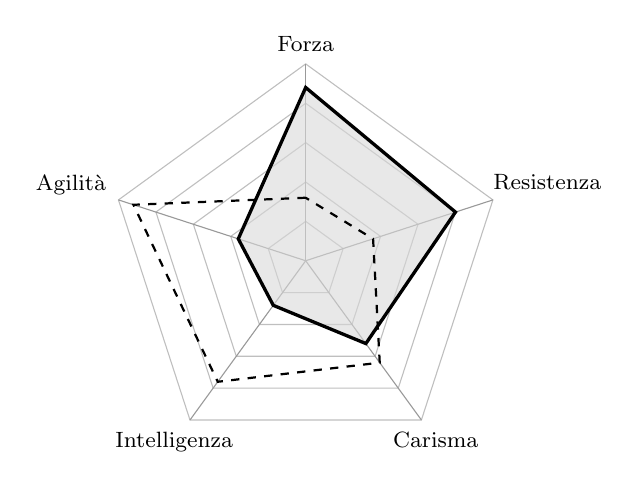
\begin{tikzpicture}[font=\footnotesize]
  \def\n{5}
  \foreach \r in {0.5,1,1.5,2,2.5} {
    \draw[black!25] (90:\r)
      \foreach \i in {1,...,4} { -- (90+\i*72:\r) } -- cycle;}
  \foreach \i/\lab in {0/Forza,1/Agilità,2/Intelligenza,3/Carisma,
                       4/Resistenza} {
    \draw[black!40] (0,0) -- (90+\i*72:2.5);
    \node[anchor=270+\i*72, inner sep=3pt] at (90+\i*72:2.55) {\lab};}
  \draw[very thick, fill=black!15, fill opacity=0.6]
    (90:2.2) -- (162:0.9) -- (234:0.7) -- (306:1.3) -- (18:2.0) -- cycle;
  \draw[thick, dashed]
    (90:0.8) -- (162:2.3) -- (234:1.9) -- (306:1.6) -- (18:0.9) -- cycle;
\end{tikzpicture}
\caption{Un grafico a radar con due profili di personaggio (valori
inventati): a colpo d'occhio si vede in quali categorie qualitative ciascuno
è spiccato.}
\label{fig:radar}
\end{figure}

\subsection{Il grafico a corde}

Nel \textbf{grafico a corde} (\emph{chord diagram}) ogni corda ha
un'\textbf{entrata} e un'\textbf{uscita}, indicata dalla punta della freccia.
L'esempio della slide mostra le \textbf{migrazioni globali} nel corso del
tempo.

\paragraph{Le relazioni tra sistemi.} Questo grafico è estremamente utile
quando si parla di \textbf{relazioni tra sistemi}. Si mettono a grafico tutti
i sistemi del gioco: il \emph{weather system}, il \emph{combat system}, gli
NPC, la vita sociale, e così via. Si mostra quanto sono collegati e in che
direzione (in un senso o in entrambi), e già a livello visivo si fa vedere
quanto, per esempio, il combattimento è collegato a tutto il resto, o quanto
un sistema invece è poco impattante e interessa relativamente meno. È un
altro modo per \textbf{mostrare} graficamente, invece di dover scrivere in
maniera esagerata, le relazioni tra i sistemi.

``Di grafici ce ne sono davvero tantissimi.'' Sta al designer imparare a
scegliere, come sempre, \emph{the right tool for the right job}; ``in questo
caso, \emph{the best tool for the right job}''.

% ---------------------------------------------------------------------
\section{La campagna di Russia in un grafico}
\label{sec:minard}

\subsection{Due avvertenze}

Per mostrare fin dove ci si può spingere, il docente ripropone un grafico già
intravisto, ``fichissimo, cioè per me è fichissimo'', con due avvertenze.
\begin{enumerate}
  \item Probabilmente lo si rivedrà al \textbf{terzo anno}, e verrà rifatta la
        stessa domanda: che cosa mostra? Ma il docente ``non cede di un
        passo'' e lo mostra lo stesso al primo anno, perché ``è troppo
        bello''. Al terzo anno, ``non mentite: noi lo sappiamo''.
  \item Il grafico è legato al \textbf{design}: fa parte di quel processo di
        \textbf{semplificazione} e di resa più grafica dei documenti di cui
        si sta parlando nelle lezioni di documentazione, e tornerà quando si
        parlerà di uno specifico tipo di documento, la ``summa'', il fine
        ultimo di questo processo.
\end{enumerate}

Il grafico viene attribuito a \textbf{Edward Tufte}, ``probabilmente il padre
delle infografiche'': ha dato i principi di base, alcuni dei quali sono
golden rules della documentazione (sezione~\ref{sec:golden-rules}), e sono
presi come base per fare UX e UI.\footnote{La mappa è in realtà opera
dell'ingegnere francese \textbf{Charles Joseph Minard} (1869). È stato Tufte,
in \emph{The Visual Display of Quantitative Information} (1983), a renderla
celebre, definendola probabilmente il miglior grafico statistico mai
disegnato.} Il docente darà poi il link a un talk che ne parla, ``uno dei
talk più belli che siano mai stati fatti sul design in generale, sul game
design in generale. A me ha aperto la mente.''

\subsection{Che cosa mostra?}

La regola del gioco: niente ``furia'', non si va a cercare che cos'è. Più ci
si spreme le meningi, più ritorno si avrà dopo. Si sa solo che è una
\textbf{variante del diagramma di Sankey}. E bisogna leggere il grafico, non i
testi (``sennò è troppo semplice'').

\begin{description}
  \item[Valerio] Potrebbe mostrare \textbf{scelte narrative} che proseguono
        con la storia. ``In questo caso no. Però è interessante: c'è un
        certo tipo di \textbf{progressione} in questo grafico.'' E, ammette il
        docente, ``ho mentito: sono due grafici'', uno sopra e uno sotto, che
        si legano tra loro.
  \item[Lorenzo] Sembra esserci una \textbf{correlazione} tra i due. La
        banda color ocra all'inizio è il 100\%; poi una parte si stacca, e
        nel tempo, procedendo, la quantità cambia, forse in un tempo comune
        alle due curve rappresentato da quella sotto. Nella banda nera si
        discrimina un'altra popolazione che si prende un'altra fetta. E
        quindi non sono percentuali ma \textbf{quantità}, perché nel tempo
        entrambe \textbf{diminuiscono}. ``Questo te lo confermo.'' Sembra uno
        strumento per analizzare più categorie e quantità correlate nel
        tempo. Il docente conferma la direzione: c'è una progressione,
        ``tra l'altro fisica''; la banda si rompe in quella nera, le
        quantità di entrambe diminuiscono, e c'è la correlazione con il
        grafico sotto, che è un \textbf{grafico a linea delle temperature}.
        Dalla classe si nota anche che la banda nera sembra ingrossarsi a
        spese dell'altra, e qualcuno azzarda un'ipotesi: petrolio bruciato e
        anidride carbonica emessa.
\end{description}

Il docente indica allora alcune linee sottili, ``con una forma che
sicuramente in vita vostra avete già visto''. Curve di livello? ``No, sono
troppo irregolari.'' Confini geografici? Una mappa delle temperature locali in
2D? Nessuno azzarda: sono \textbf{fiumi}.

\subsection{La risposta}

Il grafico mostra la quantità di uomini nell'\textbf{esercito di Napoleone
durante la campagna di Russia}, verso Mosca.
\begin{itemize}
  \item La banda chiara è la \textbf{marcia di andata}, quella nera la
        \textbf{ritirata}.
  \item La \textbf{larghezza} della banda è la grandezza dell'esercito.
  \item Durante la marcia alcuni se ne vanno: l'esercito si divide, alcuni
        tornano indietro, altri vanno avanti.
  \item In corrispondenza di un fiume si vede la banda assottigliarsi
        drasticamente: lì sono morti moltissimi uomini (``adesso io ci
        rido, ma non fa ridere'').
  \item Tutto in relazione alla \textbf{temperatura} in quei punti, che è il
        secondo grafico, sotto.
\end{itemize}

Per il docente ``è una figata'' perché, una volta letta la legenda,
\textbf{comunica immediatamente}, con un impatto grafico fortissimo, dove è
andato quell'esercito, che cosa ha vissuto, come si è piano piano non solo
separato ma anche \textbf{decimato} nel tempo: una campagna completamente
disastrosa. ``Con i grafici potete fare questa roba qua.''

\subsection{Dalle infografiche ai documenti}

In futuro si vedrà che lo stesso si può fare anche con la documentazione,
benché con i documenti di design sia veramente difficile: nella sua massima
espressione, \textbf{compressi in una singola pagina}. È il motivo per cui
Tufte è stato preso ad esempio e riadattato all'arte del documentare da
\textbf{Stone Librande}, il designer di \emph{Spore}, dei \emph{Sims} e di
altri titoli.\footnote{Nella trascrizione compare come ``Stanley Brandi''.
Il talk a cui il docente si riferisce è quasi certamente \emph{One-Page
Designs} di Stone Librande (GDC 2010), in cui la mappa di Minard e i principi
di Tufte sono il punto di partenza per i documenti di design di una sola
pagina.} Se ne riparlerà nella lezione di documentazione apposita. Non bisogna
raggiungere subito quel livello, ``perché è molto difficile, e non credo
nemmeno di esserci arrivato io''; ma il margine è tanto: \textbf{il tetto è
molto alto}. Si ragiona, si sperimenta, e si migliora nel tempo.

\paragraph{Approfondimento: Tufte nelle bibliografie di game design.} Tufte
compare nelle letture consigliate di entrambi i manuali del progetto.
Schell, in \emph{The Art of Game Design}, definisce \emph{The Visual Display of
Quantitative Information} ``la Bibbia (o almeno l'Antico Testamento) del
design delle interfacce grafiche'', e apre la sua lente della trasparenza
(\#62) con una citazione di Tufte: ``Per quanto bella sia la tua
interfaccia, sarebbe meglio se ce ne fosse di meno''. Brathwaite e Schreiber,
in \emph{Challenges for Game Designers}, consigliano \emph{Visual
Explanations}: per quanto si aderisca alle convenzioni di genere, sembra che
esistano solo uno o due modi di mostrare una barra della vita o il conteggio
delle munizioni; Tufte ``distrugge questa illusione'', mostrando molti modi
diversi di visualizzare un'informazione importante, con pregi e difetti di
ciascuno. È lo stesso messaggio della lezione: per ogni dato esiste un
grafico migliore degli altri, e trovarlo è parte del lavoro.

% ---------------------------------------------------------------------
\section{Principi per grafici migliori}
\label{sec:principi-grafici}

Ci sono comunque dei principi per migliorare, formattare e rendere più
visibili i dati di un grafico: le classiche regole della \textbf{Gestalt} e i
principi di design in generale. Cose che probabilmente si sanno già, ma è utile
ricordarle, e che si sono già cominciate ad applicare nella documentazione;
nei grafici le si può spingere ``all'esponenziale'', perché fare grafici è
``una pratica grafica, appunto''.
\begin{description}
  \item[Spazio negativo] Va sfruttato.
  \item[Scala] Ciò che è più grande impatta di più il lettore e viene
        percepito come più importante; ciò che è più piccolo, meno.
  \item[Gerarchia] L'ordine visivo delle informazioni.
  \item[Prossimità, forma, colore] Elementi vicini, della stessa forma o
        dello stesso colore vengono letti come un gruppo.
\end{description}

Al netto della ricerca (scoprire nuovi tipi di grafico, capire qual è il più
adatto) questa abilità si costruisce con l'\textbf{esperienza}: più grafici si
fanno, più si diventa abili, ``ancora di più rispetto alla documentazione
base, anche perché questo è documento''.

% ---------------------------------------------------------------------
\section{La matematica di base}
\label{sec:matematica-base}

\subsection{Quattro cose, da quinta elementare}

Non c'è tempo per un'altra pausa (``al massimo finiamo cinque minuti prima,
cosa che non è mai successa''), quindi si passa ai \emph{basic math
principles}. ``Qua siamo probabilmente in quinta elementare'': per chi non lo
sapesse non è un problema; le cose sono veramente quattro.

\subsection{La media}

La \textbf{media} (aritmetica) è la somma di tutti i numeri divisa per il
numero di elementi dell'insieme:
\[
  \bar{x} = \frac{x_1 + x_2 + \dots + x_n}{n} = \frac{1}{n}\sum_{i=1}^{n} x_i .
\]
``Su questo penso che nessuno abbia dei dubbi.''

\subsection{La media pesata}

Serve per alcuni framework o per alcuni calcoli in generale. Ci sono
\textbf{due modi} per farla.

\paragraph{Primo modo: pesi che sommano a uno.} Tutti i pesi sommati devono
dare \textbf{uno}, cioè il totale, il 100\%. Dati questi pesi, si
\textbf{moltiplica} ciascun valore per il rispettivo peso, ottenendo il valore
pesato, e poi si \textbf{somma}:
\[
  \bar{x}_w = \sum_{i=1}^{n} w_i\, x_i \qquad \text{con} \qquad
  \sum_{i=1}^{n} w_i = 1 .
\]

\paragraph{Secondo modo: pesi qualsiasi.} I pesi possono \textbf{non} dare il
100\%. Si moltiplica ciascun valore per il suo peso specifico, si sommano i
risultati, e la somma si divide per la \textbf{somma dei pesi}:
\[
  \bar{x}_w = \frac{\sum_{i=1}^{n} w_i\, x_i}{\sum_{i=1}^{n} w_i} .
\]
``Non è complessa, forse un passaggio in più.'' Il primo modo è un caso
particolare del secondo: se i pesi sommano a uno, il denominatore vale 1.

\paragraph{Un esempio.} Si vogliano confrontare due idee uscite dal
brainstorming dando un voto da 1 a 10 a tre criteri, con pesi diversi:
impatto (peso 3), costo contenuto (peso 2), coerenza con la visione
(peso 1). Un'idea con voti 8, 4 e 9 ha media semplice $(8+4+9)/3 = 7$, ma
media pesata
\[
  \frac{3\cdot 8 + 2\cdot 4 + 1\cdot 9}{3+2+1} = \frac{41}{6} \approx 6{,}83 .
\]
Con i pesi normalizzati ($3/6 = 0{,}5$; $2/6 \approx 0{,}33$;
$1/6 \approx 0{,}17$, che sommano a 1) si ottiene lo stesso risultato con il
primo modo. (L'esempio non è della lezione.)

\paragraph{Approfondimento: il valore atteso.} Schell (\emph{The Art of Game
Design}, capitolo~12) mostra uno degli usi più frequenti della media pesata
nel game design: il \textbf{valore atteso}, cioè la media di tutti i
risultati possibili di un'azione, pesati con la loro probabilità (pesi che,
come nel primo modo, sommano a uno). Se finendo su una casella verde si tira
un dado a sei facce e si ottengono altrettanti punti, il valore atteso è
$(1+2+3+4+5+6)/6 = 3{,}5$: è utile sapere che ogni volta, in media, si
guadagnano 3,5 punti. Con esiti non equiprobabili si pesa: tirando due dadi,
si vincono 5 dollari con un 7 o un 11 e se ne perde uno con qualsiasi altro
risultato. Le probabilità sono $6/36$ per il 7, $2/36$ per l'11 e $28/36$ per
il resto, quindi
\[
  \tfrac{6}{36}\cdot 5 + \tfrac{2}{36}\cdot 5 + \tfrac{28}{36}\cdot(-1)
  \approx 0{,}83 + 0{,}28 - 0{,}78 = 0{,}33 :
\]
alla lunga si vincono in media 33 centesimi a partita. Se vince solo il 7, il
valore atteso scende a zero (un gioco equo); se vince solo l'11, diventa
negativo ($-0{,}86$ circa). Schell ne fa una lente (\#35, \emph{The Lens of
Expected Value}): bilanciare un gioco passa spesso da conti di questo tipo.

\subsection{Le proporzioni}

L'ultima cosa è la \textbf{proporzione}: $a$ sta a $b$ come $c$ sta a $d$,
\[
  a : b = c : d ,
\]
dove $a$ e $d$ sono gli \textbf{estremi} e $b$ e $c$ i \textbf{medi}. La
proprietà fondamentale è che il prodotto dei medi è uguale al prodotto degli
estremi ($b \cdot c = a \cdot d$). Quindi:
\begin{description}
  \item[Incognita in un estremo] Si \textbf{moltiplicano i medi} e si divide
        per l'\textbf{estremo noto}. Esempio della lezione: in
        $100 : 35 = 20 : x$, i medi sono 35 e 20, l'estremo noto è 100:
        \[ x = \frac{35 \cdot 20}{100} = \frac{700}{100} = 7 . \]
        Verifica: 100 sta a 35 come 20 sta a 7.
  \item[Incognita in un medio] Si \textbf{moltiplicano gli estremi} e si
        divide per il \textbf{medio noto}. Esercizio della lezione: in
        $100 : 35 = x : 5$, gli estremi sono 100 e 5, il medio noto è 35. La
        classe risponde con il calcolo, ``500'', diviso 35:
        \[ x = \frac{100 \cdot 5}{35} = \frac{500}{35} \approx 14{,}3 , \]
        che il docente arrotonda a 14: 100 sta a 35 come (circa) 14 sta
        a 5.
\end{description}

``Avete tutte le informazioni basilari di matematica per sopravvivere alla
quinta elementare e al primo anno.''

\subsection{Che cosa verrà dopo}

Il discorso si complicherà al secondo anno, quando si parlerà di
\textbf{regressione lineare}: ma sono strumenti che servono per framework
specifici o per lavori specifici. Fare l'\textbf{economy designer} li
richiede, e anche un \textbf{data analyst} ha determinate competenze
matematiche; li si tratterà lì, punto per punto. Per ora interessa solo che
si ricordino queste quattro cose: semplici, ma ``una rinfrescata e averle lì
non vi fa male''.

% ---------------------------------------------------------------------
\section{Chiusura e prossimi appuntamenti}
\label{sec:chiusura-gd6}

La lezione è finita (``yes, abbiamo finito''), con un leggero margine di
anticipo. Il docente ricorda le scadenze:
\begin{itemize}
  \item il \textbf{production dictionary} per \textbf{lunedì 2}
        (sezione~\ref{sec:task-gd4});
  \item il \textbf{flowchart di Pac-Man} (o di \emph{Donkey Kong}) per
        \textbf{venerdì 6} (sezione~\ref{sec:task-gd6});
  \item l'altro task è già stato consegnato: il docente lo commenterà nel
        fine settimana o, al massimo, all'inizio della settimana successiva.
\end{itemize}

\paragraph{Leggere i commenti prima del 6.} Dopo che il docente avrà
commentato, bisogna \textbf{leggere i suoi commenti prima della lezione del
6}: in quella lezione si prenderà una pagina bianca e si comincerà a
documentare e a formattare la pagina insieme (sezione~\ref{sec:recap-documentazione}),
e prima di farlo è importante che il feedback ricevuto sia stato compreso.
Come detto l'altra volta, bisogna aspettare che il docente abbia commentato
tutto.

``Per lunedì portate il PC, perché Alessandro ne sarà sicuramente contento.''
I saluti sono di stagione: ``Buon Halloween! Buona festa dei morti!''

% ---------------------------------------------------------------------
\section*{Punti chiave del capitolo}
\addcontentsline{toc}{section}{Punti chiave del capitolo}

\begin{itemize}
  \item Nel \textbf{production dictionary} vanno i \textbf{nomi} unici o
        fraintendibili del gioco, spiegati in una o due righe (che cos'è una
        MT, che cos'è un tipo); il funzionamento profondo va nei documenti
        dedicati. Ordine alfabetico per leggibilità, ma le voci legate tra
        loro possono stare vicine; in ogni caso, \textbf{ordinato}.
  \item Nel brainstorming \textbf{nessuno viene fermato}, tutti parlano, si
        elenca tutto, si cercano background diversi. Un
        \textbf{facilitatore} (non un leader) fa sentire tutti ascoltati e
        tiene il brainstorming su uno scopo pratico. \textbf{Pause} e
        \textbf{cibo} riducono la tensione.
  \item Altre tecniche: circle, acting brainstorming, i \textbf{sei
        cappelli} di de Bono (partire dal verde; il nero è già giudizio),
        l'oggetto dal cappello, storyboard, domande, ``peggiore è, meglio
        è'', associative e \textbf{mind mapping}, il \textbf{TRIZ} (matrice
        di parametri, soluzione già nella cella, adatto a problemi
        fisici).
  \item Le regole di \textbf{Kawasaki} (make meaning, make mantra, next
        curve, DICEE, don't worry be crappy, hundred flowers, polarize,
        churn, niche, perfect your pitch) e lo \textbf{SCAMPER}. Il pitch si
        prova e riprova, ma \textbf{non si impara a memoria}.
  \item Dalle cento idee ad \textbf{almeno dieci}: \textbf{brainstorming
        matrix} impatto/effort, confronto, compromesso; contano anche la
        \textbf{motivazione} del team e la visione. Le idee vanno
        \textbf{distrutte}: se non si trova nessun difetto, c'è un problema.
  \item \textbf{KISS}: prototipare subito il cuore del gioco; muoversi,
        cambiare prospettiva, \textbf{rituali} che rompono la routine (il
        playtest del venerdì).
  \item Il \textbf{flowchart} è una rappresentazione grafica formalizzata di
        un processo; nasce nel software, e ai designer serve per IA,
        pipeline, game loop, sequenze di gameplay, player journey, UI.
        Serve a \textbf{mostrare invece di scrivere}.
  \item Regole: si legge \textbf{dall'alto in basso e da sinistra a
        destra}, nella direzione delle frecce; stesso livello, stessa
        gerarchia; il layout orizzontale evita il \textbf{wall of text}.
  \item Blocchi: \textbf{inizio/fine} (rettangolo arrotondato, obbligatori),
        \textbf{azione} (rettangolo), \textbf{decisione} (rombo, uscite
        sempre etichettate), \textbf{sotto-processo} (da spiegare in un altro
        flowchart), \textbf{input/output} (parallelogramma),
        \textbf{documento}.
  \item In un sistema o un loop di gioco il flusso \textbf{deve chiudersi o
        tornare indietro}: nessun ramo nel nulla. Le regole prima si
        imparano, poi si piegano (Oxenfree, il gioco di carte, Machinations,
        il behavior tree).
  \item Task: il \textbf{flowchart completo di Pac-Man} (Daniele:
        \emph{Donkey Kong}), come immagine leggibile e commentabile,
        esportata al 300--500\%, per venerdì 6.
  \item Grafici: \textbf{linea} per l'evoluzione continua e le previsioni,
        \textbf{gradini} per i salti discreti e le progressioni; barre e
        colonne (con legenda prima), istogrammi, torta e ciambella, aree,
        clustering; poi treemap, sunburst, \textbf{radar}, \textbf{corde}
        (relazioni tra sistemi) e la mappa di Minard resa celebre da Tufte.
        Il tetto è altissimo: fino ai documenti di una pagina di Librande.
  \item Matematica di base: \textbf{media}, \textbf{media pesata} (pesi che
        sommano a uno, oppure divisione per la somma dei pesi; il valore
        atteso ne è un caso), \textbf{proporzioni} (medi per medi, estremi
        per estremi).
\end{itemize}

%    \part{Laboratorio: le revisioni dei task}
%    \renewcommand{\thechapter}{R}
%    \renewcommand{\theHchapter}{R}   % solo con hyperref
%    % =====================================================================
%  Capitolo R — Gli errori nei task: revisioni, correzioni e consigli
%  del docente (capitolo "vivo", da aggiornare a ogni revisione)
%  Fonte: i documenti dei task consegnati dalla classe, con i commenti
%  di revisione di Mattia Podini (Google Docs esportati in .docx).
%  Task coperti finora:
%    T1  Arcade core elements  (revisioni del 28/10/2026, 9 documenti
%        di 8 studenti, circa 350 commenti)
%    T2  Production dictionary di un Pokémon (revisioni del 5-6/11/2026,
%        9 documenti di 9 studenti, 173 commenti del docente e 3 risposte
%        di studenti; .docx in tasks/revisionati/
%        2026-11-05_PokemonProductionDictionary/)
%    T3  TCG pain points, a gruppi (revisioni del 7/11/2026, 4 documenti
%        di 4 gruppi, 80 commenti; .docx in tasks/revisionati/
%        2026-11-07_TCGPainPoints/)
%    T4  Flowchart di Pac-Man (revisioni dell'11/11/2026, 8 consegne,
%        79 commenti: immagini commentate su Drive, PDF annotati e due
%        .docx; il task di Lorenzo in tasks/gd6-pacman-flowchart/)
%    T5  Compendium e High Vision di Metroid Dread (revisioni del
%        18/11/2026, 14 documenti di 7 studenti, 235 commenti; .docx in
%        2026_11_13_MDCompendium&HighVision/)
%    T6  Feedback ai concept art di Zoe, gioco di zombie (revisioni del
%        19/11/2026, 7 documenti, 113 commenti; il task di Lorenzo in
%        tasks/gd10-zombie-feedback/)
%
%  Pacchetti richiesti nel preambolo del libro: gli stessi di GD6
%    \usepackage[italian]{babel}, \usepackage[T1]{fontenc},
%    \usepackage[utf8]{inputenc} (solo pdfLaTeX), \usepackage{booktabs},
%    \usepackage{tikz} con le librerie di GD6 (qui servono
%    arrows.meta, positioning, calc). Nessun pacchetto nuovo.
%
%  Collocazione nel libro: una parte propria, in coda al corso, con
%  numerazione "R" (Revisioni):
%
%    \part{Il corso di Game Design}
%    ...
%    \input{GD1/GD6_brainstorming_flowchart_e_grafici}
%    \part{Laboratorio: le revisioni dei task}
%    \renewcommand{\thechapter}{R}
%    \renewcommand{\theHchapter}{R}   % solo con hyperref
%    \input{REV/GD/GDR_errori_nei_task}
%
%  Le lezioni future (GD7, GD8...) vanno inserite PRIMA di questa parte;
%  il capitolo R resta sempre l'ultimo del corso.
%
%  Etichette: prefisso "rv:" per le parti comuni (rv:sec:...), e
%  "rv:tN:" per tutto ciò che appartiene al task N (rv:t1:sec:...).
%  I rimandi verso le lezioni usano le etichette già esistenti
%  (sec:golden-rules, sec:regole-formali, sec:vocabolario, ecc.).
%
%  COME AGGIUNGERE UN NUOVO TASK REVISIONATO (procedura):
%    1. aggiungere una riga alla tabella rv:tab:task (indice dei task);
%    2. aggiornare, se servono, il registro degli avvertimenti
%       (rv:tab:avvertimenti, continuata in rv:tab:avvertimenti-t2)
%       e la checklist (rv:sec:checklist):
%       sono le uniche parti "cumulative" del capitolo;
%    3. copiare il modello commentato in fondo al file e incollarlo
%       PRIMA di "Punti chiave del capitolo", sostituendo N;
%    4. le schede per studente si generano dai .docx revisionati
%       (commento del docente + testo a cui è ancorato), si riportano
%       tutte, anche le ripetute, raggruppando quelle sullo stesso punto.
%
%  Macro locali del capitolo (definite con \providecommand qui sotto,
%  non serve toccare il preambolo):
%    \rvAvviso  -> [!]  commento con avvertimento di "non lettura" o
%                       errore definito grave dal docente
%    \rvBene    -> [+]  commento positivo
%    \rvAncora{testo}  -> il punto del documento a cui è ancorato il
%                       commento
%    \rvVuoto\   -> commento ancorato a una riga vuota o a uno spazio
%    \rvRisposta{Nome} -> commento o risposta scritta da uno studente
%                       nel thread di un commento (dal task T2)
%    \rvPresunto{testo} -> blocco a cui il commento si riferisce,
%                       ricostruito dal curatore (commenti su immagini,
%                       dal task T4)
%
%  Nota sui nomi: in coerenza con le regole del corso (i task vengono
%  condivisi con tutta la classe dopo la revisione, e "ciò che il
%  docente dice a uno vale per tutti"), gli errori sono riportati con
%  il nome di chi li ha commessi. Il punto non è chi ha sbagliato, ma
%  che cosa e perché.
% =====================================================================

\providecommand{\rvAvviso}{\textbf{[!]}}
\providecommand{\rvBene}{\textbf{[+]}}
\providecommand{\rvAncora}[1]{``\emph{#1}''\,:}
\providecommand{\rvVuoto}{\emph{(riga vuota o spazio)}\,:}
\providecommand{\rvRisposta}[1]{\emph{Commento di #1:}}
\providecommand{\rvPresunto}[1]{[\emph{presumibilmente} ``\emph{#1}'']\,:}

\chapter[Gli errori nei task]{Gli errori nei task: revisioni, correzioni
e consigli del docente}
\label{rv:cap:errori-task}

Questo capitolo è diverso da tutti gli altri. Non nasce da una lezione, ma
da ciò che succede \emph{dopo} le lezioni: i task consegnati dalla classe e i
\textbf{commenti di revisione} che il docente, Mattia Podini, lascia su ogni
documento. È un capitolo \textbf{vivo}: a ogni task revisionato se ne aggiunge
una sezione, e le parti comuni (il registro degli avvertimenti e la checklist
di consegna) vengono aggiornate di conseguenza.

Il motivo per cui esiste è una regola che il docente ha fissato il primo
giorno (sezione~\ref{sec:task-feedback}): i task vengono condivisi con tutta
la classe dopo la revisione, e \textbf{ciò che il docente dice a uno studente
vale per tutti}. Se a qualcuno viene detto ``la prossima volta non leggo il
documento'', da quel momento la regola vale per l'intera classe. Leggere solo i
propri commenti, quindi, non basta: un errore commentato sul documento di un
collega è un errore che, ripetuto, costa la \textbf{non lettura} anche a chi
non l'aveva commesso. Allo stesso modo, una riconsegna viene accettata solo se
integra anche ciò che nel frattempo è stato detto agli altri.

% ---------------------------------------------------------------------
\section{Come usare questo capitolo}
\label{rv:sec:come-usare}

\subsection{Struttura}

Il capitolo ha due livelli.
\begin{enumerate}
  \item Le parti \textbf{comuni}, valide per tutti i task, che si aggiornano
        a ogni revisione:
        \begin{itemize}
          \item il \textbf{registro degli avvertimenti}
                (sezione~\ref{rv:sec:avvertimenti}): tutte le regole il cui
                mancato rispetto, da un certo momento in poi, comporta la non
                lettura del documento o una punizione;
          \item la \textbf{checklist prima della consegna}
                (sezione~\ref{rv:sec:checklist}): le domande da farsi prima di
                consegnare qualsiasi documento, ricavate dagli errori
                effettivamente commessi.
        \end{itemize}
  \item Una sezione per \textbf{ogni task revisionato}, sempre con la stessa
        struttura:
        \begin{itemize}
          \item la consegna e il quadro delle consegne ricevute;
          \item gli errori raggruppati per \textbf{tipo} (forma, linguaggio,
                contenuto, uso del framework\dots), ciascuno con i commenti
                del docente, il perché e la correzione, con esempi;
          \item ciò che il docente ha \textbf{apprezzato}, perché anche quello
                è un'indicazione;
          \item le \textbf{schede delle singole consegne}: l'elenco completo
                dei commenti ricevuti da ogni documento, nessuno escluso.
        \end{itemize}
\end{enumerate}

\begin{table}[htbp]
  \centering
  \caption{Indice dei task revisionati.}
  \label{rv:tab:task}
  \small
  \begin{tabular}{@{}lp{2.6cm}p{3.2cm}p{2.2cm}l@{}}
    \toprule
    \textbf{N.} & \textbf{Task} & \textbf{Assegnato in} &
    \textbf{Consegne} & \textbf{Sezione} \\
    \midrule
    T1 & Arcade core elements & capitolo~\ref{cap:che-cos-e-un-gioco},
         sezione~\ref{sec:task-gd2} & 8 studenti, 9 documenti &
         \ref{rv:t1:sec:task} \\
    \addlinespace
    T2 & Production dictionary di un Pokémon & capitolo~\ref{cap:problema-soluzione},
         sezione~\ref{sec:task-gd4} & 9 studenti, 9 documenti (3 non letti) &
         \ref{rv:t2:sec:task} \\
    \addlinespace
    T3 & TCG pain points (a gruppi) & capitolo~\ref{cap:ricerca-idee},
         sezione~\ref{sec:task-gd5} & 4 gruppi, 4 documenti &
         \ref{rv:t3:sec:task} \\
    \addlinespace
    T4 & Flowchart di Pac-Man & capitolo~\ref{cap:brainstorming-flowchart},
         sezione~\ref{sec:task-gd6} & 8 consegne (1 senza nome, 1 su
         \emph{Donkey Kong}) & \ref{rv:t4:sec:task} \\
    \addlinespace
    T5 & Compendium e High Vision di \emph{Metroid Dread} &
         sezioni~\ref{gd9:sec:compendium} e~\ref{gd9:sec:vision};
         ricordato in~\ref{gd10:sec:apertura} & 7 studenti, 14 documenti &
         \ref{rv:t5:sec:task} \\
    \addlinespace
    T6 & Feedback ai concept art di \emph{Zoe} (gioco di zombie) &
         capitolo~\ref{gd10:cap:feedback},
         sezione~\ref{gd10:sec:task-zoe} & 7 studenti, 7 documenti &
         \ref{rv:t6:sec:task} \\
    \bottomrule
  \end{tabular}
\end{table}

\subsection{Legenda}

Nelle schede delle singole consegne ogni commento è riportato con il punto del
documento a cui il docente lo ha \textbf{ancorato} (il testo evidenziato), in
corsivo tra virgolette, seguito dal commento. Quando un commento ha ricevuto
risposte o aggiunte successive, queste seguono dopo ``\emph{E ancora:}''.
Quando nel thread interviene uno studente, il suo intervento è introdotto da
``\rvRisposta{Nome}'' e la replica del docente da ``\emph{Il docente:}''.
Quando il commento è ancorato a una zona di un'immagine (dal task T4, i
flowchart), il blocco a cui si riferisce è ricostruito dal curatore e indicato
con ``\rvPresunto{blocco}''. Due segni aiutano a orientarsi:
\begin{description}
  \item[\rvAvviso] il commento contiene un \textbf{avvertimento} (``la
        prossima volta non leggo'', ``errore grave'', ``non lo accetterò in
        futuro'') o una punizione: è una regola che da ora vale per tutti;
  \item[\rvBene] il commento è \textbf{positivo}: indica qualcosa da
        ripetere.
\end{description}
I commenti sono riportati \textbf{alla lettera}, con i loro refusi: sono
appunti di revisione, non testo curato. Le parti in cui questo capitolo
aggiunge una proposta propria (ad esempio le riscritture ``prima e dopo'')
sono sempre segnalate come tali, per non confonderle con la voce del docente.

\subsection{I tre livelli di gravità}

Dai commenti emerge una scala abbastanza chiara, che conviene avere in mente
leggendo il resto.
\begin{enumerate}
  \item \textbf{Errore da correggere}: il docente lo segnala (``testo
        inutile'', ``quanti e quali?'', ``spazio extra'') e si aspetta che non
        si ripeta. È la grande maggioranza dei commenti.
  \item \textbf{Errore grave o ultimo avviso}: ``prima e ultima volta che
        accetto una consegna simile'', ``la prossima volta non leggo il
        task''. Il documento è stato letto, ma la stessa cosa, al prossimo
        task, costa la non lettura.
  \item \textbf{Non lettura o punizione immediata}: il docente smette di
        leggere. Nel primo task è successo una volta sola, per l'uso della
        \textbf{parola proibita} (sezione~\ref{rv:t1:sec:linguaggio}); nel
        secondo a \textbf{tre documenti su nove}, tutti fermati al titolo per
        ragioni formali (sezione~\ref{rv:t2:sec:non-letti}). Nel quarto un
        task consegnato \textbf{incompleto} non ha ricevuto commenti di
        merito (sezione~\ref{rv:t4:sec:scope}). Nel quinto e nel sesto
        nessun documento è stato fermato; l'unico avviso, nel quinto, è
        ancora sul font (sezione~\ref{rv:t5:sec:forma}).
\end{enumerate}

% ---------------------------------------------------------------------
\section{Il registro degli avvertimenti}
\label{rv:sec:avvertimenti}

Le tabelle~\ref{rv:tab:avvertimenti} e~\ref{rv:tab:avvertimenti-t2}
raccolgono, task dopo task, tutte le regole su cui il docente ha dato un
\textbf{ultimo avviso}. Si ricordi che
valgono per \textbf{tutta la classe}, non solo per chi ha ricevuto il
commento. Molte erano già state enunciate a lezione (le golden rules e le
regole formali, sezioni~\ref{sec:golden-rules} e~\ref{sec:regole-formali});
la revisione le ha rese, per così dire, esecutive.

\begin{table}[htbp]
  \centering
  \caption{Registro degli avvertimenti (aggiornato al task T6). Nella colonna
  ``Da'' il task in cui la regola è stata richiamata; ``T2: non letto'' indica
  che la regola è già costata la non lettura di un documento.}
  \label{rv:tab:avvertimenti}
  \small
  \begin{tabular}{@{}p{5.1cm}p{1.1cm}p{5.6cm}@{}}
    \toprule
    \textbf{Regola} & \textbf{Da} & \textbf{Che cosa ha detto il docente} \\
    \midrule
    Margini 1,5 / 1,5 / 1,25 / 1,25 e font \textbf{Roboto 11} &
      T1, T2: non letto, T5 & ``La prossima volta non leggo il task'' (più
      studenti); ``prima e ultima volta che accetto una consegna simile'';
      nel T2: ``Anche se li hai impostati correttamente, i margini non sono
      stati rispettati. Non leggo''; nel T5, per una frase in un altro font:
      ``IL TESTO DEVE ESSERE IN ROBOTO 11, PENA LA NON LETTURA'' \\
    \addlinespace
    Niente \textbf{pagine o mezze pagine vuote} &
      T1 & ``Errore grave per il futuro'', ``errore grave da non ripetere,
      pena la non lettura'' \\
    \addlinespace
    Niente \textbf{wall of text} (paragrafi lunghi e fitti, documento non
    tecnico) &
      T1 & ``Dal prossimo task non leggerò una formattazione simile'',
      ``non lo accetterò in futuro'' \\
    \addlinespace
    Il documento è un \textbf{documento tecnico}, non una consegna
    accademica (niente testo con bibliografia in coda) &
      T1 & ``Dal prossimo task, una consegna simile non la leggerò e non
      avrà i miei feedback'' \\
    \addlinespace
    Si consegna con la \textbf{suite di Google} (Google Docs) &
      T1 & ``Lo leggo come prima e ultima eccezione, ma in futuro non lo
      accetterò'' \\
    \addlinespace
    Niente \textbf{colori banditi} (rosso RGB puro, giallo su bianco\dots) &
      T1, T5 & ``La prossima volta che lo vedo non leggo il documento''; nel
      T5, su un titolo in rosso: ``con il rosso RGB cammini su una pericolosa
      linea sottile'' \\
    \addlinespace
    Il documento deve essere \textbf{stampabile} &
      T1 & ``Con una consegna simile in futuro rischi la non lettura'' \\
    \addlinespace
    Elenchi rientrati più volte che \textbf{sacrificano spazio} a sinistra &
      T1 & ``Ripetere questa cosa in futuro ti costa la non lettura'' \\
    \addlinespace
    Mai far leggere \textbf{due volte la stessa cosa} (stessa tab copiata
    in due documenti) &
      T1 & ``Errore grave'' \\
    \addlinespace
    Niente parole \textbf{al limite della parola proibita}
    (``accattivante'') &
      T1 & ``Prossima volta rischi la non lettura'' \\
    \addlinespace
    \textbf{Parola proibita} (``intrattenimento'', ``divertente'' e
    simili) &
      T1 & Lettura interrotta subito e \textbf{task punitivo}: analisi dei
      core elements di Schell su \emph{Hatoful Boyfriend} \\
    \addlinespace
    \textbf{Errori grammaticali} (maiuscole incoerenti, spazi prima delle
    parentesi, accenti) &
      T1, T2 & Il docente ricorda ``la regola dei 5 errori grammaticali''; nel
      T2: ``Sei al limite del non letto per numero di errori grammaticali
      accumulati'', ``Sei al limite del non letto'' \\
    \bottomrule
  \end{tabular}
\end{table}

\begin{table}[htbp]
  \centering
  \caption{Registro degli avvertimenti (continua): le regole aggiunte dai
  task T2, T3 e T4.}
  \label{rv:tab:avvertimenti-t2}
  \small
  \begin{tabular}{@{}p{5.1cm}p{1.1cm}p{5.6cm}@{}}
    \toprule
    \textbf{Regola} & \textbf{Da} & \textbf{Che cosa ha detto il docente} \\
    \midrule
    % --- righe dei task successivi qui sotto ---
    \textbf{Testo inutile} in quantità (il lemma o il titolo ripetuti) &
      T2: non letto & ``Non leggo data la quantità di testo inutile
      presente'' \\
    \addlinespace
    Nome del file \textbf{Cognome\_\allowbreak Nome\_\allowbreak TitoloTask} &
      T2: non letto & ``Il documento non è nominato con
      Cognome\_\allowbreak Nome\_\allowbreak TitoloTask come da regole [\dots]. Non leggo'' \\
    \addlinespace
    \textbf{Limiti della consegna} (es. una pagina) &
      T2: non letto & ``Il limite della consegna era di una pagina, ne hai
      prodotte quasi due. Non leggo'' \\
    \addlinespace
    \textbf{Titolo} (o immagine di titolo) che occupa troppo spazio &
      T2 & ``Ti `mangia' almeno 1/4 del documento. Prima e ultima volta che
      leggo una consegna con un problema simile'' \\
    \addlinespace
    \textbf{Elenco puntato} che sacrifica spazio a destra &
      T2 & ``Nel miglior caso possibile, in una zona grigia delle regole. Lo
      accetto ora [\dots], non lo accetterò per task futuri'' \\
    \addlinespace
    Niente \textbf{reference o bibliografia in coda}: i link vanno dove
    servono &
      T1, T2 & ``Eliminabile''; nel T2: ``qui diventa estremamente necessario,
      sono da eliminare''; nel T3 (in una scheda separata): ``non risolve
      completamente il problema ma è la direzione corretta'' \\
    \addlinespace
    Formattazione curata anche (e soprattutto) nei \textbf{lavori di
    gruppo} &
      T3 & ``Avete svolto il task in team, e siete stati il team più
      numeroso, il risultato [\dots] è al limite dell'accettabile'' \\
    \addlinespace
    \textbf{Completare il task}: niente consegne a metà &
      T4: senza commenti & ``Mi riservo di non dare commenti ad un task
      mancante di parti fondamentali''; ``non aver terminato il task è un
      grosso problema'' \\
    \addlinespace
    Il \textbf{testo resta dentro il blocco} (flowchart, tabelle, immagini) &
      T4 & ``La prossima volta che vedo una svista simile non leggo'' \\
    \addlinespace
    Il \textbf{nome del protagonista} scritto come l'originale
    (\emph{Pac-Man}, non ``Pacman'') &
      T4 & ``Assumo che hai utilizzato una licenza artistica [\dots]. Prima e
      ultima volta'' \\
    \addlinespace
    Anche i \textbf{documenti di supporto} seguono le regole formali (niente
    note in .txt) &
      T4 & ``Perché questo documento integrativo non si presenta secondo le
      regole stabilite?''; ``anche questo deve adottare i margini e le regole
      viste a lezione'' \\
    \bottomrule
  \end{tabular}
\end{table}

\paragraph{La regola dei cinque errori grammaticali.} Nel primo task il
docente la richiama di passaggio (``ricordo la regola dei 5 errori
grammaticali''), come regola già nota: a lezione era stato detto che non
devono esserci errori grammaticali gravi e che la coerenza della lingua fa
parte della sequenza corretta di un documento
(sezione~\ref{sec:golden-rules}). La soglia esatta e la sua conseguenza non
sono esplicitate nei commenti; la lettura più prudente è considerarla un
limite oltre il quale il documento non viene letto.

% ---------------------------------------------------------------------
\section{La checklist prima della consegna}
\label{rv:sec:checklist}

Questa checklist traduce in domande gli errori commessi davvero. Va
ripercorsa \textbf{prima di ogni consegna}, su qualsiasi task. Accanto a ogni
gruppo è indicata la sezione in cui gli errori corrispondenti sono spiegati
nel dettaglio.

\subsection{Forma e regole formali}
\begin{itemize}
  \item Il file è nominato \textbf{Cognome\_\allowbreak Nome\_\allowbreak TitoloTask}? Ho
        rispettato i \textbf{limiti della consegna} (numero di pagine)?
        (\ref{rv:t2:sec:non-letti})
  \item È un \textbf{Google Doc}, con margini 1,5 sopra e sotto e 1,25 a
        sinistra e a destra, e tutto il testo in \textbf{Roboto 11}?
        (\ref{rv:t1:sec:forma})
  \item C'è qualche \textbf{pagina o mezza pagina vuota}? Qualche spazio
        sprecato in fondo a una sezione o sotto un titolo?
  \item Ho usato \textbf{righe vuote} (Invio ripetuti) per distanziare i
        paragrafi, invece dell'interlinea e dello spazio dopo il paragrafo?
  \item Il testo è \textbf{giustificato}? (Sconsigliato ``caldamente''.)
  \item C'è qualche paragrafo che, visto al 50\% di zoom, sembra un
        \textbf{muro di testo}?
  \item Qualche \textbf{tabella} o elenco è spezzato tra due pagine?
        Qualche immagine sfora i margini o è finita nella pagina dopo il
        testo che la richiama?
  \item Ci sono colori banditi, testo giallo su bianco, sfondi scuri? Il
        documento si può \textbf{stampare}?
  \item Il \textbf{titolo} dice che tipo di documento è (analisi,
        production dictionary\dots), su che gioco e, se serve, con quale
        framework? È senza ripetizioni, decorazioni e immagini che mangiano
        spazio? Le tab sono rinominate e ognuna contiene una sola cosa?
        (\ref{rv:t2:sec:forma})
  \item Elenchi puntati, sottoelenchi e colonne lasciano \textbf{spazio
        bianco a destra}? Ne vale il prezzo?
  \item Le \textbf{tabelle} arrivano ai margini, con lo spazio ripartito
        bene tra le colonne e un distacco dal testo prima e dopo? Ogni
        \textbf{immagine} porta un'informazione o è una decorazione? Il
        testo scorre attorno alle immagini invece di lasciare righe vuote?
        (\ref{rv:t3:sec:forma})
  \item C'è una sezione di \textbf{reference in coda}? (Va tolta: i link
        si mettono dove servono.)
  \item Grassetto, corsivo, sottolineato e colori seguono una
        \textbf{logica coerente} e dichiarabile?
  \item Maiuscole, punti, spazi dopo la punteggiatura e prima delle
        parentesi, parentesi chiuse: tutto in ordine?
\end{itemize}

\subsection{Linguaggio}
\begin{itemize}
  \item Ogni frase \textbf{serve}? Ho ripetuto nel testo il nome del gioco,
        del framework o della sezione che è già nel titolo?
        (\ref{rv:t1:sec:linguaggio})
  \item Ci sono \textbf{opinioni personali} (``sicuramente'', ``per me'',
        ``il migliore'') al posto di dati?
  \item Ci sono \textbf{parole deboli} (``potrebbe'', ``forse'', ``una sorta
        di'')?
  \item Ci sono aggettivi \textbf{non misurabili} (``lungo'', ``breve'',
        ``alto volume'', ``semplice'', ``molte piattaforme'') senza un metro
        di paragone o un numero?
  \item Ho scritto da \textbf{recensore} (battute, intercalari, domande
        retoriche, ``ci viene mostrato'') invece che da designer?
  \item C'è la parola proibita, o qualcosa di simile?
  \item In un elenco di voci, ogni definizione \textbf{ripete il lemma}
        (``Pokédex: il Pokédex è\dots'')? (\ref{rv:t2:sec:linguaggio})
  \item Ho scritto ``pokémon'' (o qualunque nome proprio) \textbf{sempre
        allo stesso modo}?
\end{itemize}

\subsection{Contenuto e framework}
\begin{itemize}
  \item Ho \textbf{dichiarato} il framework con il suo nome preciso (``core
        elements di Romero e Schreiber'', ``tetrade elementale di
        Schell'')? (\ref{rv:t1:sec:framework})
  \item Ogni informazione è nella \textbf{voce giusta} del framework? Ho
        nominato in una sezione qualcosa (una modalità, un sistema) mai
        spiegato nelle meccaniche?
  \item Per ogni meccanica: che cosa succede \textbf{premendo l'input}? E
        se lo si preme di nuovo? Con quali \textbf{numeri}? Che cosa succede
        al \textbf{game over} e al cambio di livello?
        (\ref{rv:t1:sec:meccaniche})
  \item Per ogni oggetto di gioco: \textbf{quanti e quali}, quando
        compaiono, che cosa fanno, che cosa succede se il personaggio ci
        entra in contatto?
  \item Ho \textbf{mostrato} (immagini, UI, sprite, tabelle) ciò che si può
        mostrare? (\ref{rv:t1:sec:mostrare})
  \item Le affermazioni su pubblico, temi, prestazioni sono sostenute da
        \textbf{dati e reference}?
  \item Ho risposto a \textbf{tutto} ciò che chiedeva la consegna?
  \item In una definizione, ogni \textbf{termine unico} che uso ha una sua
        voce? Ho detto prima \textbf{che cos'è} (statistica, edificio, key
        item, consumabile\dots), poi chi, quanti, dove, a che costo, con che
        sistema? (\ref{rv:t2:sec:voce})
  \item Ci sono generalizzazioni false (``tutti'', ``solo'', ``sempre'')?
        Due voci dicono cose diverse sulla stessa cosa?
  \item Se c'è un limite di spazio: \textbf{ogni riga lavora}? Avanza spazio
        mentre alcune voci restano stringate? Posso accorpare voci simili?
        (\ref{rv:t2:sec:priorita})
\end{itemize}

\subsection{Dati, analisi e design}
\begin{itemize}
  \item Ogni problema è sostenuto da \textbf{dati} e dalla \textbf{voce
        degli utenti}, mostrata e linkata nel punto in cui serve? I criteri
        con cui ho scelto i problemi sono misurabili?
        (\ref{rv:t3:sec:dati})
  \item Il problema è \textbf{specifico}? Ho trovato il problema più grave
        e la sua \textbf{causa}, non solo il sintomo? I competitor sono
        nominati e confrontati per intero? (\ref{rv:t3:sec:analisi})
  \item Ogni soluzione ha un \textbf{esempio concreto}, dei \textbf{numeri}
        (anche tentativi) e, se tocca l'interfaccia, un \textbf{mockup} o
        wireframe? (\ref{rv:t3:sec:design})
  \item Ho provato a rompere la soluzione con i \textbf{casi limite}? Ne ho
        dichiarato costi, conseguenze, pro e contro rispetto alle
        alternative? È ancora coerente con l'identità del gioco?
  \item Nelle proposte c'è \textbf{linguaggio debole} (``si potrebbe'',
        ``may'')?
\end{itemize}

\subsection{Flowchart}
\begin{itemize}
  \item Da ogni \textbf{rettangolo} esce \textbf{una sola freccia}? Se le
        strade sono più d'una, ho usato un rombo? Se le azioni sono più
        d'una, le ho messe in sequenza? (\ref{rv:t4:sec:regole})
  \item Ogni uscita di ogni \textbf{rombo} è etichettata, con un esito
        diverso dalle altre (niente due ``sì'')? Il ``sì'' e il ``no'' sono
        dalla parte giusta?
  \item Ogni \textbf{sotto-processo} ha il suo flowchart? L'ordine dei
        sotto-processi segue l'ordine causale (prima ci si muove, poi si
        mangia)?
  \item Qualche freccia si \textbf{sovrappone} o si incrocia in modo
        fraintendibile? Qualche blocco è \textbf{scollegato} (``nothing
        happens'')? Ho seguito a mano ogni loop?
  \item Se un programmatore implementasse il flowchart così com'è, il gioco
        funzionerebbe? (\ref{rv:t4:sec:logica})
  \item Vite rimaste, vite guadagnate, \textbf{game over}, \textbf{high
        score}, passaggio di livello: ci sono tutti?
  \item Ho dato i \textbf{numeri} (durate, punteggi, liste di oggetti) o
        rimandato a una tabella che li contiene?
  \item Il testo è di \textbf{una sola misura} e sta \textbf{dentro} i
        blocchi? Il nome del gioco e del protagonista è scritto giusto?
        (\ref{rv:t4:sec:forma})
  \item L'immagine si legge senza zoomare (esportazione al 300--500\%)? I
        documenti di supporto rispettano le regole formali?
  \item Ho deciso \textbf{prima} la profondità che posso permettermi con il
        tempo che ho? Il task è \textbf{completo}, e coerente nella profondità
        delle sue parti? (\ref{rv:t4:sec:scope})
\end{itemize}

\subsection{Compendium e vision}
\begin{itemize}
  \item Il compendium ha la \textbf{legenda degli status}? Ogni status dice
        chi approva e che cosa è successo al documento (scritto, approvato,
        implementato, testato)? Ci sono status senza una differenza
        pratica tra loro? (\ref{rv:t5:sec:compendium})
  \item Le categorie sono i \textbf{dipartimenti operativi}? Ogni documento
        sta in una categoria? Ogni sistema ha il suo documento? Ho messo
        nel compendium cose che stanno in engine?
  \item I \textbf{pilastri} valgono per tutto il gioco e promettono sistemi
        che esistono? Sono ad alto livello, senza nomi e numeri che si
        decideranno in produzione, ma con abbastanza informazione?
        (\ref{rv:t5:sec:pilastri})
  \item Ci sono \textbf{tre} prime emotions e \textbf{tre} prime moods,
        ciascuno giustificato?
  \item Il \textbf{must do} risponde al ``livello vuoto di Unreal'': 3C,
        nemici unici e la loro IA, boss, abilità, progressione, mappa? O è
        solo stile artistico? (\ref{rv:t5:sec:design})
  \item Il \textbf{must not} esclude tentazioni plausibili, o nega il must
        do, o dice ciò che si assume di base? Il \textbf{nice to have} è
        davvero tagliabile?
  \item Al massimo \textbf{tre USP}, ognuno davvero unico, senza varianti
        dello stesso sistema? (\ref{rv:t5:sec:usp})
  \item La vision è di tutto il team (niente nome dell'autore)? Le
        informazioni sono in testo modificabile, non in immagini?
        (\ref{rv:t5:sec:forma})
\end{itemize}

\subsection{Feedback}
\begin{itemize}
  \item Ho ripreso il \textbf{mandate} (o la visione) e ogni rilievo vi fa
        riferimento? (\ref{rv:t6:sec:mandate})
  \item Ci sono \textbf{giudizi} (``great'', ``buono'', ``ben'', ``nice'')
        al posto del rapporto con il mandate? Parole deboli (``could be'',
        ``not sure'') o troppo forti? (\ref{rv:t6:sec:giudizio})
  \item Ogni problema ha \textbf{la sua soluzione}, specifica e legata a
        quel problema? Ho rimandato all'artista domande che posso
        risolvere io come designer? (\ref{rv:t6:sec:soluzione})
  \item Ogni richiesta ha una \textbf{reference}? Posso mostrare la
        soluzione sull'immagine (cerchi, mashup)?
        (\ref{rv:t6:sec:reference})
  \item Ho stimato il \textbf{costo} di ciò che chiedo? Ho coinvolto chi
        deve decidere con me? Lascio aperta la possibilità di iterare?
        (\ref{rv:t6:sec:lead})
  \item Uso il lessico del corso nel suo senso tecnico (\emph{submission},
        \emph{fiero})?
\end{itemize}

% =====================================================================
\section{Task 1 --- Arcade core elements}
\label{rv:t1:sec:task}

\subsection{La consegna}

Il task era stato assegnato alla fine della lezione su che cos'è un gioco
(sezione~\ref{sec:task-gd2}) e confermato in quella successiva:
\begin{enumerate}
  \item scegliere un \textbf{gioco arcade};
  \item scegliere \textbf{uno} dei framework visti a lezione (Schell, Romero
        e Schreiber, oppure Bura) e analizzare il gioco con quello;
  \item far emergere le \textbf{tre emozioni} principali verso cui il gioco
        è orientato, con il vocabolario visto in aula;
  \item aggiungere una \textbf{propria definizione di gioco arcade};
\end{enumerate}
con il vincolo dei termini banditi e, nella lezione sulla documentazione,
le regole formali di consegna (sezione~\ref{sec:regole-formali}). Era il
\textbf{primo task} di documentazione del corso, e il docente lo ricorda più
volte nei commenti: diverse cose vengono ``accettate per ora'', ma con
l'avvertimento che dal task successivo non lo saranno più.

\subsection{Le consegne in sintesi}

\begin{table}[htbp]
  \centering
  \caption{Le consegne del task T1.}
  \label{rv:t1:tab:consegne}
  \small
  \begin{tabular}{@{}p{2.3cm}p{2.7cm}p{2.4cm}p{3.9cm}@{}}
    \toprule
    \textbf{Studente} & \textbf{Gioco} & \textbf{Framework} &
    \textbf{Il nodo principale} \\
    \midrule
    Francesca Attadia & \emph{Bubble Bobble} (1986) & Schell &
      Buon primo tentativo; meccaniche poco dettagliate \\
    \addlinespace
    Antonino Etiopia & \emph{Top Gear} & Romero e Schreiber (core
      elements, non nominati) & Elenchi rientrati che sprecano spazio; dati
      sui giocatori assenti \\
    \addlinespace
    Federica Ferrara & \emph{Geometry Dash} (2013) & Schell &
      Margini errati; domanda sull'arcade lasciata senza risposta; tono da
      recensore \\
    \addlinespace
    Mattia Maestri & \emph{Donkey Kong} (1981) & non dichiarato &
      Margini, font e rosso RGB; framework incompleto; manca la definizione
      di arcade \\
    \addlinespace
    Francesco Muratore & \emph{Pac-Man} & Schell \emph{e} Romero e
      Schreiber nella stessa tab & Margini; wall of text; linguaggio debole;
      tecnologia fraintesa \\
    \addlinespace
    Alberto Maria Ronchi & \emph{Tetris} & Schell (non nominato) &
      Margini; meccanica confusa con strategia; definizione che si
      contraddice \\
    \addlinespace
    Valerio Rossaro & \emph{Dino Rex} (1992) e \emph{Punch-Out!!} (1984),
      due documenti & non dichiarato & Wall of text; stessa tab ripetuta
      in due documenti; \textbf{parola proibita} \\
    \addlinespace
    Lorenzo Vergata & \emph{Jet Set Radio}, \emph{Crazy Taxi 2},
      \emph{The Legend of Valkyrie} & Schell, Romero e Schreiber, Bura &
      Documento accademico e non tecnico, in inglese, fuori dalla suite
      Google; definizione troppo larga \\
    \bottomrule
  \end{tabular}
\end{table}

Il quadro che ne esce è netto. Quasi tutti gli errori ricadono in quattro
famiglie, nell'ordine di frequenza:
\begin{enumerate}
  \item \textbf{testo inutile} e scrittura poco puntuale (opinioni, parole
        deboli, aggettivi non misurati);
  \item \textbf{impaginazione}: spazi vuoti, righe vuote al posto
        dell'interlinea, margini e font, muri di testo;
  \item \textbf{meccaniche descritte ad alto livello}, quando l'analisi
        richiede un dettaglio ``a basso livello'';
  \item \textbf{uso del framework}: informazioni nella voce sbagliata,
        voci mancanti, framework non dichiarato.
\end{enumerate}
Le prossime sezioni li affrontano uno per uno.

% ---------------------------------------------------------------------
\subsection{Errori di forma e di impaginazione}
\label{rv:t1:sec:forma}

\paragraph{Margini e font.} È l'errore più ``economico'' da evitare ed è
anche quello su cui il docente è più netto. Quattro documenti su otto non
avevano i margini stabiliti (1,5 sopra e sotto, 1,25 ai lati) e uno non era in
Roboto:
\begin{quote}
  ``Il documento non ha i margini corretti e il font non è Roboto. Prima e
  ultima volta che accetto una consegna simile.'' (Mattia)\\
  ``I margini del documento non sono quelli stabiliti, la prossima volta non
  leggo il task.'' (Francesco, Alberto)\\
  ``Hai sfruttato correttamente le tab del documento, ma i margini non sono
  quelli stabiliti. La prossima volta non leggerò il documento se ripeterai
  l'errore.'' (Federica)
\end{quote}
\emph{Correzione}: impostare margini e Roboto 11 come predefiniti
\textbf{prima} di scrivere (Google Docs lo permette: File, Impostazione
pagina, ``Imposta come predefinito''), e ricontrollarli prima di consegnare.

\paragraph{Lo spazio sprecato.} Il commento più ricorrente sulla forma, in
tutte le sue varianti: ``spazio extra'', ``doppio spazio'', ``mezza pagina
bianca qui sotto, è spazio sprecato'', ``praticamente una pagina di spazio
sprecato'', ``qui sotto c'è una pagina intera di spazio sprecato, per il
futuro è considerato un errore grave''. Lo spazio, a lezione, era stato
definito ``oro'', ``come l'acqua nel deserto'' (sezione~\ref{sec:golden-rules}).
I casi visti nel primo task:
\begin{itemize}
  \item \textbf{mezza pagina o pagina vuota in coda} al documento o a una
        tab (Antonino, Federica, Mattia, Alberto, Lorenzo): errore grave;
  \item \textbf{una pagina usata per una battuta}: Lorenzo apre la seconda
        parte con un finto ``esempio perfetto'' (\emph{Michael Jackson's
        Moonwalker}) seguito da ``no, ok, just kidding'': ``hai buttato una
        pagina per un joke: non è un pitch'';
  \item \textbf{una pagina usata per un passaggio di sezione} (``let's
        continue with the next game''): ``per fare questo perdi una pagina di
        spazio completamente sprecato'';
  \item \textbf{titoli sviluppati in verticale}, che lasciano vuoti i lati
        (Mattia: ``il titolo è esteso verticalmente, troppo, considerando lo
        spazio che perdi sui lati'');
  \item \textbf{elenchi rientrati tre volte}, che mangiano tutto il margine
        sinistro (Antonino: ``questa cosa può funzionare per alcuni
        paragrafi, ma su tutto il documento no. Hai sacrificato molto spazio
        a sinistra, ripetere questa cosa in futuro ti costa la non
        lettura'');
  \item \textbf{spazio a destra di un elenco} lasciato vuoto quando poteva
        ospitare un'immagine (Mattia: ``hai ampio spazio qui sulla destra
        dell'elenco puntato'').
\end{itemize}

\paragraph{Le righe vuote al posto dell'interlinea.} Un commento ripetuto
identico su cinque documenti: ``Invece delle spaziature, sfrutta gli strumenti
di Google come l'interlinea o lo spazio dopo il testo personalizzato. Vale per
ogni uso di spazio simile, per rompere il testo, nell'intero documento.''
Premere Invio due volte per staccare i paragrafi produce spazi irregolari,
che si spostano a ogni modifica e finiscono in cima alle pagine. Lo strumento
giusto è \textbf{Formato, Interlinea e spaziatura paragrafo}, con uno
``spazio dopo'' personalizzato, applicato in modo uniforme (meglio ancora se
salvato negli stili dei titoli e del testo normale).

\paragraph{Il testo giustificato.} ``Sconsiglio caldamente l'uso del testo
giustificato, in generale'' (Federica, Valerio, Lorenzo). In un documento
tecnico, in colonne strette e con molti termini lunghi o inglesi, la
giustificazione crea spazi irregolari tra le parole e rende la lettura più
faticosa. Si allinea a sinistra.

\paragraph{Il wall of text.} È la forma che il docente ha bocciato con più
decisione, e che dal secondo task non verrà più letta:
\begin{quote}
  ``Questa pagina è tutto wall of text, dal prossimo task non leggerò una
  formattazione simile.'' (Francesco)\\
  ``Tutto il documento è un pericoloso wall of text con leggibilità ridotta,
  riflettici attentamente perché in futuro non accetterò una formattazione
  simile.'' (Valerio, \emph{Dino Rex})\\
  ``Questa formattazione è un grave wall of text. Non lo accetterò in
  futuro.'' (Valerio, \emph{Punch-Out!!})
\end{quote}
Il caso di \emph{Punch-Out!!} mostra bene il meccanismo: in un solo blocco
finiscono la presentazione del gioco, l'obiettivo, lo scopo della singola
partita e il pubblico di riferimento. ``Questo è un altro punto, argomento,
paragrafo. Unire tutto insieme riduce drasticamente la leggibilità.''
\emph{Correzione}: un paragrafo, un argomento; elenchi puntati quando le voci
sono parallele (``tutto questo può tranquillamente essere messo a elenco
puntato migliorandone la leggibilità''); titoli o grassetti che permettano a
chi legge di saltare direttamente al punto che gli interessa.

\paragraph{Documento tecnico, non accademico.} Il documento di Lorenzo
(\emph{The Ingredients of Tasteful Arcade Games}) è il caso limite: una
ricerca ampia e corretta, con fonti accademiche, ma impaginata come un
saggio, in inglese, con la bibliografia in coda e, per di più, non in Google
Docs.
\begin{quote}
  ``Questo non è un documento tecnico: è un wall of text con reference in
  coda, più simile ad una consegna accademica, e non è l'obiettivo di un Game
  Designer. Dal prossimo task, una consegna simile non la leggerò e non avrà
  i miei feedback.''
\end{quote}
Il punto non è la quantità di lavoro (il docente si dice ``personalmente
contento di vedere lavoro extra''), ma il rapporto tra forma e fruibilità:
``quello che guadagni in contenuto lo perdi in forma [\dots]: il rischio (e il
risultato qui) è un documento non tecnico dalla ridotta leggibilità, che un
domani nessuno leggerà veramente. O peggio, lo leggeranno dimenticandosi cosa
implementare o cosa era importante.'' Le reference, poi, vanno
\textbf{linkate nel punto in cui servono}: una bibliografia finale è
``eliminabile, me li hai linkati dove era necessario''.

\paragraph{Prima l'MVP, poi l'extra.} Dallo stesso documento viene una regola
generale: ``prima di espandere la consegna la \emph{rule of thumb} è iterare
sull'MVP''. Analizzare tre giochi con tre framework, quando la consegna ne
chiede uno, ha senso solo se l'analisi richiesta è già impeccabile; altrimenti
moltiplica i difetti.

\paragraph{Tabelle spezzate e scorrimento.} ``Mai, e dico mai, rompere una
tabella in più pagine.'' Allo stesso modo, ``stai rompendo il discorso in due
pagine, cosa da evitare assolutamente''. Sulla matrice di Bura di Lorenzo il
docente aggiunge un'osservazione di metodo che vale per ogni documento:
\begin{quote}
  ``Il lettore è qui, sta leggendo la riga e vuole vedere dove era nella
  matrice di Bura. Per come hai formattato, deve continuamente fare su e giù,
  potenzialmente dimenticandosi pezzi nel mentre. A questo non sempre c'è una
  soluzione ideale, o non è sempre necessario che ci sia, però sono dettagli
  sui quali devi pensare adesso. Perché dedicare tempo e attenzione ora ti
  renderà un GD poi.''
\end{quote}

\paragraph{Immagini: dove e come.} Le immagini sono incoraggiate (si veda la
sezione~\ref{rv:t1:sec:mostrare}), ma devono stare \textbf{dentro i margini}
(``l'immagine sotto non rispetta i margini, è un dettaglio assolutamente
evitabile'') e \textbf{accanto al testo che le richiama}: a Federica ``le
immagini sono cadute nella pagina seguente, intuizione corretta ma
applicazione da rivedere''. Un'immagine usata come titolo grafico non è
sbagliata, ma va ragionata rispetto allo spazio e al titolo testuale già
presente (Antonino).

\paragraph{Colori.} Mattia ha scritto il titolo in \textbf{rosso RGB puro}:
``citato come colore bandito nelle slide sulla documentazione. La prossima
volta che lo vedo non leggo il documento''. Francesco ha usato il
\textbf{giallo su bianco}: ``poco leggibile''. Valerio ha consegnato un
documento \textbf{non stampabile}: ``con una consegna simile in
futuro rischi la non lettura''. Anche i link rossi di Lorenzo sono ``non
comuni, ma borderline accettabili'': il link deve distinguersi, ma senza
uscire dalla palette.

\paragraph{Formattazione senza logica.} Ad Antonino: ``inizio ad avere
difficoltà a capire come hai scelto grassetto, italico e sottolineatura:
perché mi sembra che il risultato sia il medesimo, far risaltare elementi
importanti.'' Se tre strumenti fanno la stessa cosa, il lettore non impara a
leggerli. Ogni stile deve avere \textbf{un significato}, sempre lo stesso.

\paragraph{Il titolo e l'apertura.} Il titolo deve dire, in un colpo
d'occhio, \textbf{che documento è}, \textbf{su che cosa} e \textbf{con quale
framework}:
\begin{itemize}
  \item ``Che tipo di documento è? Design? Analisi? Secondo che framework?
        Mancano informazioni cruciali'' (Mattia; identico a Valerio);
  \item ``Il titolo appare più come una recensione piuttosto che un documento
        tecnico di analisi, inoltre è immotivatamente schiacciato a destra''
        (Lorenzo);
  \item positivo: ``pur non osando con immagini, il titolo rimane essenziale e
        presenta tutti gli elementi necessari. Funziona'' (Francesca);
        ``titolo funzionale'' (Federica, \emph{Geometry Dash --- Core
        Elements --- Jesse Schell}).
\end{itemize}
Anche le \textbf{intestazioni interne} devono pesare per quello che sono:
``Brenda Romero \& Ian Schreiber's'' scritto a 11 punti ``apre il doc, non
può essere a 11 di grandezza, deve essere rilevante per il lettore''; e il
passaggio dalla definizione di arcade al framework ``deve chiaramente
presentarsi come divisore''.

\paragraph{Le tab.} Le tab di Google Docs servono a \textbf{separare parti
diverse} dello stesso documento: ``l'utilità di avere più tab è proprio quella
di dividere parti differenti dello stesso doc, qui hai Schell e di là
Romero+Schreiber'' (Francesco, che li aveva messi insieme). Ogni tab ha un
titolo (``manca il titolo della tab'', Valerio) e va pensato
\textbf{l'ordine}: la definizione di arcade di Alberto era nell'ultima tab,
``questa tab avrei dovuto leggerla prima, non dopo''. E soprattutto: ``mai
fare leggere al lettore due volte la stessa cosa'' (Valerio aveva copiato la
stessa tab sulla definizione di arcade in entrambi i documenti).

\paragraph{Punteggiatura e refusi.} Maiuscole mancate (``Top gear'', ``n'' a
inizio frase, ``Donkey kong''), punto mancante, spazio mancante prima di una
parentesi o dopo un punto, parentesi chiusa ma mai aperta, ``Un'altro''.
A Francesco, che apre e chiude le citazioni digitando due apostrofi di
seguito, il docente ricorda: ``usa la punteggiatura specifica quando
possibile''. Ciascuno di questi, preso da solo, è minimo; ma rientrano tutti
nella regola dei cinque errori grammaticali.

% ---------------------------------------------------------------------
\subsection{Errori di scrittura e di linguaggio}
\label{rv:t1:sec:linguaggio}

\paragraph{``Testo inutile''.} È, di gran lunga, il commento più frequente
del primo task: compare su \textbf{tutti} i documenti, decine di volte (``ma
questo errore è presente più volte di quante io ne possa realisticamente
commentare''). Le forme ricorrenti:
\begin{itemize}
  \item \textbf{ripetere il titolo}: ``Analisi del gioco Top Gear'' sotto il
        titolo, ``Pac-Man'' come soggetto di ogni sezione, ``Donkey Kong è
        un gioco arcade [\dots] nato nel 1981'' quando titolo e anno sono già
        in testa (``lo hai scritto già sopra''); ``testo inutile, il gioco è
        rimasto lo stesso'';
  \item \textbf{annunciare invece di dire}: ``nel gioco sono presenti diverse
        meccaniche:'', ``Ci sono diverse regole imposte dal sistema di gioco''
        (``testo inutile, cita le regole invece di scrivere questo''),
        ``Top Gear presenta una serie di regole utili'', ``Il sistema di
        gioco mette a disposizione del giocatore una serie di comandi'';
  \item \textbf{ripetere l'etichetta della sezione}: ``La narrativa racconta
        di'', ``Dal punto di vista narrativo'', ``Il target di riferimento
        era'', ``L'obiettivo in Donkey Kong è'', ``Sta giocando al gioco
        un'', ``La tecnologia scelta'';
  \item \textbf{rimandi a sé stessi}: ``(come sopra citato)'': ``allora non
        dirlo''; ``As said at the beginning of this work'': ``allora è inutile
        se lo hai già detto'';
  \item \textbf{premesse e congedi}: ``Ok, then. Excuse me for this long
        introduction'' (``non è scusabile''), ``That's it for now. Bye! :)''
        (``ahimè, testo inutile'');
  \item \textbf{l'assunto}: frasi che ripetono ciò che la consegna già dà per
        scontato (``Using the vocabulary seen in class, Jet Set Radio, for me,
        is oriented towards four emotions:'': ``questo è l'assunto, tutto
        evitabile'').
\end{itemize}
\emph{Il test}: se cancello la frase, il lettore perde un'informazione? Se
no, la frase va cancellata. Un esempio, dalla consegna di Mattia:

\begin{center}
\small
\begin{tabular}{@{}p{0.46\textwidth}p{0.46\textwidth}@{}}
  \toprule
  \textbf{Nella consegna} & \textbf{Riscrittura proposta} \\
  \midrule
  \emph{Meccaniche.} Nel gioco sono presenti diverse meccaniche:
  \emph{Punteggio.} Il punteggio in Donkey Kong viene assegnato al
  giocatore in base alle azioni intraprese da quest'ultimo durante la
  partita.
  &
  \emph{Punteggio.} Contatore sempre visibile nella UI [immagine con il
  contatore evidenziato], che aumenta in base alle azioni compiute nel
  quadro (tabella sotto). \\
  \bottomrule
\end{tabular}
\end{center}
\noindent La riscrittura è costruita sulla definizione che il docente stesso
dà nel commento: ``sistema che incrementa sulla base di azioni compiute nel
quadro, aggiornando un contatore sempre presente nella UI''.

\paragraph{Opinioni personali.} ``Al limite dell'opinione personale'' è il
secondo commento più frequente. Esempi: ``sicuramente'' (``Ciò che attrae di
più di Pac-Man sono sicuramente''), ``una difficoltà moderata'', ``in Top Gear
ci sono poche risorse'', ``molto semplice'', ``the perfect example'',
``first position in my heart'', ``I consider myself a good Mario Kart
gamer'' (``opinione personale. Non può stare qui''), ``assordante''
(``opinione personale, non hai portato né dati né reference''). Un'opinione
può diventare un'affermazione accettabile solo se è sostenuta da dati o
reference; altrimenti si toglie.

\paragraph{Parole deboli.} ``Niente linguaggio debole. Stai scrivendo un
documento di analisi, sii certo di quello che inserisci e di come lo dici''
(Francesco, su ``potrebbe avere''). Stessa sorte per ``potrebbero essere'',
``una persona potrebbe tranquillamente essere attratta'' (``linguaggio
debole, tutto evitabile'') e per ``I would'' (Lorenzo). È la regola delle
golden rules: se il dato è quello, si scrive il dato
(sezione~\ref{sec:golden-rules}).

\paragraph{Aggettivi senza metro.} Il docente li segnala uno per uno, quasi
sempre con la stessa domanda: \emph{rispetto a che cosa?}
\begin{itemize}
  \item ``breve durata delle partite'': ``relativo. Serve un metro di
        paragone'';
  \item ``alto volume'': ``da capire cosa significhi `alto' '';
  \item ``lunghe corse'': ``serve un metro di misura, al limite
        dell'opinione personale'';
  \item ``semplicità del gameplay e immediatezza del gioco'': ``da definire
        `semplice' e `immediato' '';
  \item ``prettamente semplici da memorizzare'': ``senza un metro di misura
        questa è una opinione personale'';
  \item ``vecchio gioco arcade'': ``cosa significa questo?'';
  \item ``per molto tempo'': ``generico'';
  \item ``molte altre piattaforme'', ``numerosissime piattaforme'': ``non
        `molte altre', `le seguenti', quelle che elenchi sotto. Sii
        puntuale'';
  \item ``sacrificando un po' di tempo'': ``quantità specifica, anche con un
        margine di errore va bene'';
  \item ``per un tot di secondi'': ``ok, prossimo step: esplicitare questo
        parametro'';
  \item ``rigidità'': ``non significa nulla così''.
\end{itemize}
\emph{Correzione}: un numero (anche approssimato, ``circa 3 secondi''), un
confronto esplicito (``partite di 2--5 minuti, contro le decine di minuti di
una sessione console''), oppure un elenco completo al posto di
``molti''.

\paragraph{Il tono da recensore.} Un documento di analisi non è una
recensione né un pezzo per un blog. Il docente lo segnala in molte forme:
\begin{itemize}
  \item domande retoriche e ``azzardi'' dichiarati: ``Innanzitutto, perché
        proprio Geometry Dash? perché questa scelta così azzardata?''
        (Federica): ``questa è una frase da `recensore'. Quello che scrivi
        nella descrizione già dovrebbe incorporare questo tuo `azzardo',
        dissipando ogni potenziale dubbio. [\dots] Sono le spiegazioni
        concrete qua sotto e il loro legame che implicitamente ti definiscono
        come Designer'';
  \item il ``noi'' e il ``ci'' rivolti al lettore: ``Ci viene mostrato un
        mondo'': ``può esserti utile mettere della distanza tra te e il
        lettore: allena anche l'oggettività mettendo da parte l'ego'';
  \item intercalari e battute: ``I mean'' (``nessun intercalare, non sei un
        recensore videoludico''), ``(blasphemous)'' (``inutile e fuori
        luogo''), ``Do we have to put in our dish we're cooking drugs?
        [\dots]'' (``commenti del genere non hanno spazio dentro documenti di
        analisi e/o design''), la playlist suggerita per la lettura
        (``soluzione interessante, ma discutibilmente fuori luogo per un
        documento di analisi'');
  \item formule che promettono sintesi e non la mantengono: ``Long story
        short'' seguito da un paragrafo lungo: ``questo è proprio falso'';
  \item il ``per me'' e il ``LA MIA definizione'': ``chiaro, il documento ha
        il tuo nome'' (Alberto); ``for me the most important of all'':
        ``tutto eliminabile, motivalo e basta'' (Lorenzo).
\end{itemize}

\paragraph{Frasi impersonali e soggetti vaghi.} ``Una volta che si è riusciti
a prenderle'': ``Chi? Il giocatore? Il main character? Perché la frase è
impersonale?'' In un documento tecnico il soggetto di ogni azione deve essere
esplicito: \textbf{il giocatore} preme un input, \textbf{il main character}
compie l'azione, \textbf{il sistema} reagisce.

\paragraph{Il tempo verbale.} A Valerio, che descrive gli arcade solo al
passato: ``continui a parlare al passato, e nel presente?'' Una definizione
di genere deve reggere anche oggi.

\paragraph{Stereotipi.} Sul passaggio in cui il mondo arcade viene
definito ``\emph{stereotypically male-oriented}'', il commento è secco: ``cosa da evitare''.

\paragraph{La parola proibita.} È l'unico caso, nel primo task, di
\textbf{lettura interrotta}. Nel documento su \emph{Punch-Out!!} Valerio
scrive che il pubblico di riferimento ``cercava un \emph{intrattenimento} più
rapido'':
\begin{quote}
  ``Inaccettabile, smetto di leggere questo documento. Come punizione devi
  produrre una analisi dei core elements di Schell su \emph{Hatoful
  Boyfriend}, per lunedì 9 novembre.''
\end{quote}
La regola era stata data alla seconda lezione
(sezione~\ref{sec:vocabolario}): niente ``divertente'', ``intrattenente'' e
varianti, perché non dicono \emph{perché} un gioco funziona; e la punizione di
Mattia Podini è proprio un'analisi su un gioco ``terribile'', fino a
\emph{Hatoful Boyfriend}. Attenzione anche ai \textbf{dintorni} della parola:
a Francesca, per ``accattivante'', il docente scrive ``al limite della parola
proibita, prossima volta rischi la non lettura''. La correzione è sempre la
stessa: nominare l'\textbf{emozione} o la \textbf{qualità} precisa (sfida,
tensione, \emph{fiero}, ritmo, leggibilità\dots) con il vocabolario visto in
aula.

\paragraph{Usare il vocabolario del corso.} Il docente corregge anche le
parole quasi giuste: ``frustrazione e soddisfazione'' $\rightarrow$
``\emph{fiero} è la parola che cerchi'' (Federica); ``competizione
amichevole'' $\rightarrow$ ``Cooperative, Fellowship, People Fun. Ne
riparleremo'' (Francesca); ``stunts'' $\rightarrow$ ``ad alto livello, questo
è un combo system'' (Lorenzo). Su ``dynamics'', usato da Lorenzo per indicare
le sezioni a ritmo serrato, il docente scrive ``termine inesatto perché ha
una sua controparte più largamente accettata'', senza dire quale; ``ci
ritorneremo''.\footnote{Nota del curatore: il termine a cui il docente
allude non è esplicitato nel commento. Da tenere d'occhio nelle prossime
lezioni.}

% ---------------------------------------------------------------------
\subsection{La definizione di gioco arcade}
\label{rv:t1:sec:arcade}

Era una parte esplicita della consegna, e i commenti ne fanno emergere sei
errori tipici.
\begin{enumerate}
  \item \textbf{Mancare la definizione.} Mattia scrive soltanto che
        \emph{Donkey Kong} ``è un gioco arcade'': ``spiegare cosa significa
        era parte del task''.
  \item \textbf{Porre la domanda senza rispondere.} Federica chiude il
        paragrafo con ``La domanda è: ad oggi, un gioco platform può essere
        considerato anche arcade?'': ``ok, ma mi devi rispondere tu,
        altrimenti il doc è amputato''.
  \item \textbf{Contraddirsi.} Alberto definisce gli arcade come i giochi
        ``nati per essere giocati nei cabinati'' e subito dopo aggiunge
        ``anche se ora i cabinati sono tecnologia obsoleta'': ``allora stai
        già confutando la tua stessa tesi''.
  \item \textbf{Usare parole vuote.} ``Gli arcade possono per esempio essere
        giochi con meccaniche semplici'': ``questo non significa nulla preso
        da solo''. E sugli esempi moderni che seguono: ``Hades ha
        `meccaniche semplici'? UFO 50 ha letteralmente 50 titoli con
        meccaniche diverse, dovremmo prenderli singolarmente [\dots] o
        considerarli un unico titolo?''
  \item \textbf{Definire troppo largo.} Lorenzo propone due definizioni di
        gioco (``A packaged state of mind that aims to give [\dots] chosen
        experiences''; ``A juicy interaction infused with conflict'') e il
        docente le smonta con controesempi: ``secondo questa definizione,
        Journey è un arcade''; ``secondo questa definizione, Call of Duty è
        un arcade''; e Flower, che Lorenzo stesso mette tra i ``definitely
        not'', rientrerebbe nella prima. ``Comprendi che un risultato simile
        non è, purtroppo, accettabile date le premesse.'' Anche il criterio
        ``reducing randomness to the lowest possible levels'' cade su un
        controesempio: ``diresti che Vampire Survivors non è arcade?''
  \item \textbf{Fermarsi al passato.} Valerio descrive bene i cabinati degli
        anni '70--'90, ma ``continui a parlare al passato, e nel presente?'';
        e ``difficile ma facile da capire, con pochi comandi e tasti, e
        partite molto veloci'' richiede ``più informazioni specifiche''.
\end{enumerate}

\paragraph{Il controesempio come strumento.} Il metodo del docente è lo stesso
visto a lezione sulle definizioni di gioco
(capitolo~\ref{cap:che-cos-e-un-gioco}): ogni definizione include qualcosa ed
esclude qualcos'altro, e la si mette alla prova cercando un gioco che la
rispetta pur non essendo, evidentemente, ciò che si vuole definire. Prima di
consegnare una definizione, conviene fare da sé questo esercizio con due o
tre titoli noti.

\paragraph{Dati grezzi e sintesi.} Il documento di Lorenzo parte da una
ricerca ampia (fonti accademiche, storia dei cabinati, caratteristiche del
genere), e il docente lo riconosce: ``questa ricerca porta tutti dati utili
nella definizione ultima''. Il problema è che ``restano dati grezzi'': ``la
fase di selezione e spogliatura del non essenziale non è sufficiente. Il
risultato sono due pagine di testo saltabile e una definizione di una pagina
che è un wall of text''. E più avanti: ``quindi concretamente cosa è emerso da
questo paragrafo di mezza pagina? Nessun punto critico che compone la tua
ipotetica definizione finale.'' Chi legge vuole arrivare alla definizione
``vuoi per praticità, vuoi per tempistiche'': la ricerca va
\textbf{distillata}, e in apertura serve sintesi (``io sono d'accordo con
quello che scrivi, ma domandati come puoi essere più sintetico in
apertura'').

\paragraph{Che cosa ha funzionato.} Francesca include il ``sistema di
memorizzazione dei punteggi migliori per stimolare la competizione tra i
giocatori'': ``formulato correttamente''. Federica sposta il criterio dal
luogo all'esperienza (``non è più il luogo in sé a definire il genere'',
``almeno, non solo quello, ma sono d'accordo''), e il porting di
\emph{Geometry Dash} su cabinato ``solidifica la tua tesi''. Sui legami tra
arcade, slot machine e coin-op, il docente corregge Lorenzo in modo
istruttivo: l'associazione non deriva dai giochi d'azzardo, ma ``a monte, dallo
sfruttare bias cognitivi per la manipolazione del giocatore (senza entrare in
discorsi etici)''; e la presenza maschile citata dagli studi è ``legata
principalmente alla posizione dei coin-op in passato''. Infine, una domanda
lasciata aperta: se un gioco qualsiasi diventa arcade quando è giocato in un
cabinato, ``la ritualità di una macchina con elementi fisici/meccanici è una
discriminante? Non dico che sia sbagliato, ma apre possibilità
discutibili''.

% ---------------------------------------------------------------------
\subsection{Dichiarare e usare il framework}
\label{rv:t1:sec:framework}

\paragraph{Dire quale framework.} ``Quale framework? Non ne esiste solo uno
legato a loro. Parliamo dei Core Elements'' (Antonino, su ``framework di
Romero e Schreiber''); ``quale? Non ne esiste solo uno'' (Alberto); ``il
framework resta quello dei core elements, da dire'' (Lorenzo). Mattia e
Valerio non lo dichiarano affatto. Il nome preciso va nel titolo o subito
sotto: ``Core elements (Romero e Schreiber)'', ``Tetrade elementale
(Schell)'', ``Matrice di Bura''. I framework sono descritti nel
capitolo~\ref{cap:che-cos-e-un-gioco} (sezioni~\ref{sec:schell},
\ref{sec:romero-schreiber} e~\ref{sec:bura}).

\paragraph{Ogni cosa nella sua voce.} Molti commenti spostano
un'informazione nella voce corretta del framework:
\begin{itemize}
  \item ``Questa è una dinamica legata alle regole dello spazio di gioco,
        andava associata alle regole'' (Francesca, sul passaggio dal fondo
        alla cima dello schermo);
  \item ``Obiettivo: sarebbe stato utile inserirlo nel paragrafo delle
        meccaniche'' (Mattia);
  \item ``Va spiegato prima'' (Valerio, sull'obiettivo arrivato a metà
        pagina); ``mai parlato dello spazio di gioco prima di adesso, a metà
        della prima pagina'';
  \item ``Ti avrebbe potuto aiutare descrivere lo spazio di gioco all'inizio
        delle regole?'' (Antonino);
  \item ``Davvero è rilevante per il documento, in un elenco sulle risorse
        (e non, per esempio, nelle regole)?'' (Antonino, sul consiglio di
        usare il nitro con parsimonia);
  \item ``Non stai parlando di narrativa, stai parlando di estetiche qui''
        (Lorenzo, sulle influenze dell'art director);
  \item ``Ha l'intera libertà di movimento'', scritto nella narrativa:
        ``meccanica, da riformulare in ogni caso'' (Francesco); ``a ogni
        reset il gioco è sempre più difficile'': ``come? Questa è una
        meccanica''.
\end{itemize}

\paragraph{Niente che non sia stato introdotto.} Un elemento citato in una
voce deve essere stato spiegato prima, nella voce che gli compete. ``Super
Mode: mai parlato di questa modalità nelle meccaniche''; ``punti: mai parlato
di un sistema di punti, della coop locale né dell'high score''; ``boss
finale: di cui non so le meccaniche associate'' (Francesca); ``se prendi
l'ultima bacca rimanente nel livello, questo si resetterà: purtroppo mai
citato prima'' (Francesco); ``sistema di leaderboard da spiegare sopra''
(Alberto); ``Peccato non aver citato la bidimensionalità nelle meccaniche e
nelle estetiche'' (Federica, che la cita solo nella tecnologia).

\paragraph{La tecnologia, per Schell.} Francesco, sotto ``Tecnologia'',
descrive il movimento nel labirinto e i tunnel laterali: ``quello che descrivi
non è la tecnologia per Schell: dove gira Pac-Man? Su che piattaforme è
disponibile? Quali sono i controlli fisici del gioco?'' La stessa domanda
torna ovunque: ``cabinati con comandi fisici: quali? E ora, dove viene giocato
o riprodotto?'' (Francesca); ``da cabinato di tipo upright. E ora? Su che
macchine gira?'' (Mattia). La tecnologia è \textbf{hardware, piattaforme
(allora e oggi), controlli fisici}, e i limiti o le possibilità che ne
derivano. Ogni affermazione tecnica va verificata: ``con immediatezza e senza
troppo input lag: da verificare e validare''; ``molto semplice [il
crossplatform]: opinione del gioco, non hai mai parlato del codice
dell'applicazione''. E ogni dettaglio va pesato rispetto all'analisi: i sequel
su NES, Super Nintendo e Wii di \emph{Punch-Out!!} sono ``un dettaglio utile
all'analisi tramite core elements? Domandatelo''.

\paragraph{I sistemi di gioco.} Mattia scrive che i sistemi di gioco
``sono quelli di arrivare a fine livello collezionando più punti possibile'':
``No, i sistemi di gioco sono collezioni di meccaniche mirate allo stesso
obiettivo: il sistema di punteggio, gli ostacoli di gioco, la locomozione del
main character.''

\paragraph{Meccanica o strategia?} Alberto descrive la meccanica di
\emph{Tetris} come ``incastrare pezzi senza lasciare spazi vuoti per
completare le righe'': ``non è una meccanica questa, è una strategia''. Il
docente riscrive (si veda l'esempio nella
sezione~\ref{rv:t1:sec:meccaniche}).

\paragraph{Risorse e modello mentale.} Nel documento su \emph{Crazy Taxi 2},
Lorenzo inserisce tra le risorse la ``conoscenza della città'': ``non è una
risorsa in gioco, fa parte del modello mentale''. Al contrario, mancano
risorse vere: ``tempo e posizione?'' (Antonino); ``punti'' e ``punteggio'',
``altra risorsa'' (Francesco). Nella matrice di Bura di \emph{Valkyrie}, il
docente nota che la voce più importante (la clessidra) è ``in fondo
all'elenco'': l'ordine degli elenchi comunica priorità.

\paragraph{Game qualities.} Le qualità sono ``l'anima condensata del tuo
gioco'' (a chi aveva scritto ``il PvE è l'essenza del gioco''). Gli studenti
ne hanno indicate troppo poche. Ad Antonino: ``puoi pensarne altri, come per
esempio la camera di gioco''; ``scalare le classifiche [\dots] può
tranquillamente essere un'altra qualità''; il sistema di password ``andrebbe
citato nelle qualità del gioco''. A Francesco, che indica solo il PvE: ``ci
sono altri elementi: Arcade, Top-Down Third Person. Ripensaci''. A Lorenzo,
che raggruppa i verbi in sistemi: ``queste sono più qualità messe insieme,
eppure non info sulle 3C del gioco'' (camera, character, controls).
``Elementi fisici'', detto delle bacche di \emph{Pac-Man}, è impreciso: ``non
seguono regole fisiche''.

\paragraph{Players: servono dati.} Nessuno ha portato dati sul pubblico, e il
commento è sistematico: ``servono i dati'', ``fascia di età'' (Antonino);
``qual è la fascia di età? La demografica dei giocatori? I dati?''
(Francesco); ``No. Non ci sono dati sulle demografiche: etnia, genere,
segmenti di età, etc.'' (Lorenzo). Il docente riconosce che gli archetipi di
giocatori non sono ancora stati spiegati (``non avendo ancora visto
(giustamente) archetipi di giocatori non puoi semplificare chiaramente il
concetto''), ma le affermazioni sul pubblico (``probabilmente perché ha poco
tempo da spendere sui videogiochi'') vanno sostenute da fonti.

\paragraph{Temi e obiettivi.} Ad Antonino: ``per quello che scrivi, c'è anche
un tema riguardo alla competizione e alla scalata della vetta agonistica''.
Sull'obiettivo, a Federica: ``l'obiettivo (meccanico e narrativo) resta
arrivare alla fine [del livello] tutto d'un pezzo''.

\paragraph{Le emozioni.} Erano parte della consegna. A Lorenzo, che elenca
``Auditory/visual stimulation'' e ``Challenge'' senza commento: ``nessuna
spiegazione, nemmeno per challenge?'' Ogni emozione va \textbf{motivata} con
gli elementi del gioco che la producono, come il docente fa a Francesco:
eccitazione e competizione ``corretto, dato da elementi quali il chasing dei
fantasmi, il time clock, la leaderboard''.

% ---------------------------------------------------------------------
\subsection{Descrivere le meccaniche: il dettaglio richiesto}
\label{rv:t1:sec:meccaniche}

Il problema di contenuto più diffuso è uno: le meccaniche sono descritte
\textbf{come le descriverebbe un giocatore} a un amico, non come le deve
descrivere un designer a un team che dovrà ricostruirle. Il docente lo dice
nel commento ad Alberto: ``l'analisi presuppone un dettaglio a basso
livello''. E a Francesca suggerisce un metodo: ``un modo per aiutare la
comprensione è quello di partire dall'obiettivo e poi andare sempre più in
dettaglio sulle meccaniche'' (lo stesso approccio che, a Francesco, giudica
funzionante: ``iniziare con l'obiettivo può funzionare se stai descrivendo le
meccaniche'').

\begin{figure}[htbp]
  \centering
  \begin{tikzpicture}[
      node distance=4mm,
      box/.style={draw, rounded corners=2pt, align=center,
                  text width=2.25cm, minimum height=1.25cm,
                  font=\footnotesize},
      arr/.style={-{Stealth[length=2mm]}, thick}]
    \node[box] (obj) {\textbf{Obiettivo}\\ come si vince, come si perde};
    \node[box, right=of obj] (spa) {\textbf{Spazio}\\ quadro, tile, limiti, UI};
    \node[box, right=of spa] (ogg) {\textbf{Oggetti}\\ quanti, quali, quando};
    \node[box, right=of ogg] (inp) {\textbf{Input e verbi}\\ che cosa succede premendo};
    \node[box, below=9mm of inp] (sta) {\textbf{Stati e parametri}\\ durate, velocità, numeri};
    \node[box, left=of sta] (int) {\textbf{Interazioni}\\ contatto, collisione};
    \node[box, left=of int] (sis) {\textbf{Sistemi}\\ punteggio, vite, livelli};
    \node[box, left=of sis] (esi) {\textbf{Esiti}\\ game over, quadro successivo};
    \draw[arr] (obj) -- (spa);
    \draw[arr] (spa) -- (ogg);
    \draw[arr] (ogg) -- (inp);
    \draw[arr] (inp) -- (sta);
    \draw[arr] (sta) -- (int);
    \draw[arr] (int) -- (sis);
    \draw[arr] (sis) -- (esi);
  \end{tikzpicture}
  \caption{Dall'obiettivo al dettaglio: un ordine possibile per descrivere le
  meccaniche, ricostruito dalle domande che il docente pone nelle revisioni
  del task T1 (proposta del curatore, non uno schema mostrato a lezione).}
  \label{rv:t1:fig:dettaglio}
\end{figure}

\paragraph{Le domande del docente.} Raccolte e raggruppate, le domande poste
nei commenti formano una vera checklist di analisi. Conviene porsele per ogni
meccanica, prima di consegnare.

\begin{description}
  \item[Input] ``Cosa succede praticamente quando il giocatore preme il
        tasto? Quale effetto ha sul main character?'' (Mattia, sul salto);
        ``Se il main character sta compiendo un salto, e il giocatore preme
        di nuovo l'input associato, cosa succede?'' (Francesca); ``Con che
        input? Cosa succede durante l'azione `scalare'?'' (Mattia, sulle
        scale); ``Come si compie questa azione di `raccogliere'?''
        (Francesco); ``Invece lato input di gioco?''; ``Riguardo agli input
        coinvolti?'' (Antonino); ``E gli input lato giocatore/macchina?''
        (Lorenzo). Anche gli stati cambiano l'input: in \emph{Geometry
        Dash} volare, cambiare forma e invertire la gravità sono ``tutti
        verbi di gioco da spiegare nel dettaglio, perché con lo stesso input
        il risultato cambia a seconda dello stato attuale del main
        character''.
  \item[Movimento e limiti] ``Muoversi liberamente'': ``Falso. [\dots] Se il
        giocatore si muove contro un muro? Può muoversi verso l'alto senza
        saltare?'' (Francesca); ``Allora non è `libero'. E se finisce in un
        `buco' ai limiti dello spazio fisico del gioco?'' (Francesco);
        ``Quanto posso uscire dal tracciato?'' (Antonino); ``Va descritto
        anche cosa significa `partire' ''; ``va descritto il sistema di
        accelerazione e velocità generale''.
  \item[Oggetti e nemici] ``Quanti e quali'' (ripetuto più volte);
        ``Quando vengono droppati? Che oggetti sono? Come si ottengono e come
        si usano?''; ``Stanno fermi? Si muovono? Hanno comportamenti unici?''
        (Francesca, sui nemici); ``Come si muove la polizia, che azioni ha a
        disposizione, che interazione può compiere o subire'' (Lorenzo);
        ``Mancano elementi chiave come ostacoli, NPC. Cosa popola il mondo di
        gioco?''; ``ombrello, cappello, borsa: in quanto lettore, non so cosa
        siano questi vantaggi''; ``spawn: non so quale sia né dove sia''.
  \item[Collisioni] ``Per ciascuno [oggetto], cosa succede se il giocatore
        ci collide?'' (Federica).
  \item[Parametri] ``Tot di secondi: esplicitare questo parametro''; ``300,
        500, 800: da spiegare''; ``4 o più barili: contemporaneamente o in
        lasso di tempo definito?''; ``determinato numero: quante?'';
        ``determinato numero di punti: quanti? Link alla tabella della
        wiki''; ``velocità della caduta: ok, ma puoi essere più specifico'';
        ``colpi critici: cosa significa? Che regole hanno?''.
  \item[Sistemi] ``Da spiegare il sistema di livelli, high score e game
        over''; ``dunque esiste un sistema di tempo, da spiegare'';
        ``punti: sistema da spiegare, come quello dei livelli''; ``i punti
        collezionati: sono mostrati da qualche parte? Aumentano in tempo
        reale?''; ``vite: come lo `uccidono' e cosa succede a queste
        `vite'?''; ``checkpoints: che cosa sono? Come funzionano?''.
  \item[Esiti] ``Ora so che il gioco si basa su livelli, ma non so cosa
        succede quando uno finisce e uno nuovo inizia''; ``cosa succede dopo
        il game over?''; ``manca l'outcome del game over: dove viene
        riportato il giocatore?''; ``cosa comporta il game over''; ``cosa
        significa `game over'?''; ``si resetterà: cosa significa a livello
        pratico?''; ``round: come vengono segnate [le vittorie]? Dove?''.
\end{description}

\paragraph{La core mechanic va trovata.} Su \emph{Tetris} il docente
riscrive di persona il cuore dell'analisi di Alberto. È l'esempio migliore di
che cosa si intende per ``basso livello'':

\begin{center}
\small
\begin{tabular}{@{}p{0.46\textwidth}p{0.46\textwidth}@{}}
  \toprule
  \textbf{Nella consegna} & \textbf{Riscrittura del docente} \\
  \midrule
  La meccanica base del gioco è incastrare pezzi (tetramini) l'uno con
  l'altro, senza lasciare spazi vuoti per completare le righe, una volta che
  una riga viene completata sparisce dando dei punti.
  &
  ``La core mechanic è spostare/ruotare il tetramino assegnato. Una volta
  posizionato, un nuovo tetramino viene generato e assegnato. Ci sono altre
  meccaniche: la UI che mostra il prossimo tetramino che verrà generato, il
  sistema di despawn delle righe (e quello di punteggio, che va spiegato), e
  così via.'' \\
  \bottomrule
\end{tabular}
\end{center}

\noindent Lo stesso Alberto, poco sotto, aveva colto il punto: le rotazioni e
gli spostamenti ``possono essere eseguiti tutte le volte desiderate, a una
condizione, ovvero quella di farlo prima che avvenga un contatto con altri
tetramini'': ``corretto, ecco le tue core mechanic''. E ancora, per
\emph{Bubble Bobble}: ``sparare bolle: questa meccanica (quella core)
necessita di maggiori dettagli''.

\paragraph{Un esempio da riscrivere: il cambio di stato.} Su \emph{Pac-Man}
il docente abbozza la forma che la descrizione dovrebbe avere: ``meccanica da
spiegare: Pac-Man cambia stato per N secondi, così come i fantasmi che
avranno come nuovo obiettivo fuggire da lui [\dots]. Va spiegato, nel
dettaglio.'' Sviluppando lo schema (proposta del curatore):

\begin{center}
\small
\begin{tabular}{@{}p{0.46\textwidth}p{0.46\textwidth}@{}}
  \toprule
  \textbf{Nella consegna} & \textbf{Riscrittura proposta} \\
  \midrule
  All'interno del mondo di gioco sono presenti anche delle bacche speciali,
  che rendono il giocatore ``ostile'' verso i fantasmi. Una volta raggiunto
  uno, questo non scomparirà, ma tornerà al proprio punto di spawn. (Per
  ogni fantasma catturato, vengono attribuiti 200/400/600/800 punti in più).
  &
  \emph{Power pellet} (4 per quadro, agli angoli del labirinto
  [immagine]). Al contatto con Pac-Man:
  \begin{itemize}
    \item Pac-Man entra nello stato \emph{potenziato} per N secondi (N
          diminuisce con il livello);
    \item i fantasmi passano allo stato \emph{spaventato}: cambiano sprite,
          rallentano, invertono la direzione e fuggono;
    \item al contatto con un fantasma spaventato, il fantasma torna alla
          casa al centro del labirinto e il giocatore guadagna 200, 400,
          800, 1600 punti per fantasma consecutivo.
  \end{itemize} \\
  \bottomrule
\end{tabular}
\end{center}

\noindent Si noti che la riscrittura risponde, una per una, alle domande del
docente: ``catturato: non ho idea di come farlo, come lettore'' (al
contatto), ``spawn: non so quale sia né dove sia'' (la casa al centro),
``determinato: quante?'' (4).\footnote{Nota del curatore: nella consegna i
punti per fantasma erano indicati come 200/400/600/800; i valori del gioco
originale sono 200, 400, 800 e 1600, raddoppiati a ogni fantasma mangiato con
lo stesso power pellet. È esattamente il tipo di dato per cui il docente
chiede il ``link alla tabella della wiki''.}

\paragraph{Riassunti corretti, ma non abbastanza.} Il docente riconosce più
volte un buon riassunto, chiedendo però di scendere di livello: ``tutta
questa sezione è un corretto riassunto delle meccaniche di Geometry Dash, ma
puoi essere più specifica sui singoli elementi [\dots]. Tutte domande che
determinano la profondità dell'analisi'' (Federica); ``corretto. Avrei voluto
leggere di più a riguardo'' (Francesca, sul salto sulle bolle). Il riassunto
è il punto di partenza, non il punto d'arrivo.

% ---------------------------------------------------------------------
\subsection{Narrativa, estetiche e tecnologia}
\label{rv:t1:sec:narrativa}

\paragraph{La trama in 5W+H.} A Francesca (\emph{Bubble Bobble}): ``prova a
rispondere alle 5W+H'' (\emph{who, what, when, where, why} e \emph{how}),
e poi ``un paio di righe in meno e ci siamo come riassunto''. A Lorenzo, su
una trama di \emph{Jet Set Radio} lunga e piena di nomi propri: ``tutto
questo va riassunto con 5W+H''. Il riferimento positivo è la riga che la
precede: ``JSR has a linear and scripted narrative, served in small portions
between levels by DJ Professor K'': ``questo è corretto, preciso, succinto.
Parti da questo''. Anche il riassunto di Valerio su \emph{Dino Rex} riceve
``sintetico, funziona''.

\paragraph{Il tipo di narrativa.} Va detto: a Mattia, ``manca il tipo di
narrativa, che è lineare''; Francesca la dichiara (``ramificata, con tre
finali'') e i finali sono apprezzati come approfondimento sulla morale e
sull'intento di design (``ottimo'').

\paragraph{``Non c'è storia'' non è mai vero.} ``There is no real story'':
``questo non è mai vero, capisco quello che intendi ma va riformulato''
(Lorenzo). Allo stesso modo, ``non racconta direttamente'' ``andrà formulato
diversamente'' (Federica, rimandato alle lezioni di narrativa). Anche quando
il gioco non ha una trama esplicita, la narrativa passa da altri canali:
``indubbiamente la cover art e la scocca del cabinato possono dare
informazioni sulla narrativa di gioco, pensa a Space Invaders dove il tema è
tutto `spiegato' lì'' (Alberto). Le letture personali (\emph{Tetris} come
``conflitto infinito tra caos e ordine'') sono ammesse solo con dati: ``una
tua lettura, alla quale posso pure venire incontro, ma servono i dati''; e
``molti designer'': ``chi? Dove sono i dati?''.

\paragraph{Estetiche: concrete, non impressioni.} Le estetiche sono state
descritte quasi sempre per impressioni (``colorata e saturata'',
``giocosità'', ``colori accesi'', ``colorato e sgargiante''). Il docente
chiede ogni volta l'elemento concreto:
\begin{itemize}
  \item \textbf{palette} (``palette principale?''), \textbf{stile artistico}
        (``perché? Parla dello stile artistico, anche sinteticamente'');
  \item \textbf{UI} (``mancano elementi come lo stile della UI, gli SFX'';
        ``puoi parlare anche della UI qui'');
  \item \textbf{audio}: stile della colonna sonora, BPM, SFX (``continui a
        non darmi informazioni estetiche sullo stile della colonna sonora, per
        esempio i BPM, e anche degli SFX'');
  \item \textbf{reference}: ``esempi, reference, link''; ``esempi concreti,
        immagini''; ``dati, reference''; ``corretto, ma le reference?''.
\end{itemize}
Le affermazioni devono corrispondere alle reference: ``sanguinano
copiosamente: in nessuna delle immagini che hai inserito c'è un rivolo di
sangue''. E vanno contestualizzate storicamente: ``fotorealistica: questo
dipende dal contesto storico, detto adesso è falso''. Anche la lettura
``soulful graphics'' di Lorenzo è ``inquantificabile rispetto anche alle
tecnologie usate oggi, in contrapposizione al tubo catodico ormai desueto'':
una tecnica nata da limiti che oggi non esistono più. Mattia, infine, aveva
omesso del tutto le estetiche: ``mancano le estetiche''.

\paragraph{Tecnologia.} Si veda la sezione~\ref{rv:t1:sec:framework}: per
Schell è hardware, piattaforme e controlli fisici, allora e oggi. Il
``feeling'' dei comandi fisici è ``da approfondire''; le piattaforme vanno
elencate (o linkate, se sono molte: ``quale delle N versioni portatili? Puoi
anche linkare una pagina''); l'interpretazione dei fatti va evitata (``limitava
il giocatore, perché non poteva giocarci dove voleva'': ``al limite della tua
interpretazione dei fatti''). Bene, invece, la socialità del co-op ``spalla a
spalla'' (Francesca: ``questo invece è corretto'') e il pubblico dietro al
cabinato (Lorenzo: ``interessante, mi trovi d'accordo'').

% ---------------------------------------------------------------------
\subsection{Mostrare invece di scrivere}
\label{rv:t1:sec:mostrare}

``Dovrei vederlo, non leggerlo.'' La prima golden rule
(sezione~\ref{sec:golden-rules}) torna in decine di commenti:
\begin{itemize}
  \item la UI e il punteggio: ``puoi anche lavorare sulle immagini di gioco,
        mostrando chiaramente dove sia questo punteggio a schermo'';
        ``barra della salute: come sono fatte? Ce ne sono più di una? Di che
        altri elementi si compone la UI?'';
  \item gli sprite: ``come lettore dovrei vedere questi sprite'';
  \item le peculiarità visive: ``quello inferiore dedicato all'incontro: perché
        non lo mostri?''; ``come una figura trasparente di spalle: da vedere.
        Uguale per gli oggetti di gioco, lavora sulle immagini'';
  \item i comandi: ``assolutamente corretto, ma come puoi mostrarlo senza
        scriverlo così?'' (un'immagine del pannello di controllo con le
        funzioni sui tasti dice tutto in meno spazio).
\end{itemize}

\paragraph{Tabelle e matrici.} Quando i dati sono confrontabili, vanno
\textbf{tabellati}. Ad Antonino, sulle quattro statistiche delle auto
(velocità massima, accelerazione, grip, consumo): ``prova a pensare a come
sarebbero potute essere ancora più visibili come informazioni''; e su 8
nazioni $\times$ 4 gare: ``ora immagina come avresti potuto condensare tutto,
risparmiando spazio e scrivendo di meno, però con un risultato ancora più
chiaro per il lettore''. A Lorenzo, sul controllo finale della sua ``ricetta''
arcade: ``come avresti potuto rendere questo una matrice/tabella visivamente
chiara e compatta nel doc?''. L'idea delle catene causa--effetto con le
frecce (``Crazy Hop $\rightarrow$ shorter route $\rightarrow$ \dots'') è invece
``interessante, iteraci sopra'': è già un flowchart in forma testuale.

\paragraph{Immagini che lavorano.} Quando l'immagine c'è ed è al posto
giusto, il docente lo nota: l'elenco dei personaggi di Francesca ``già così è
molto chiaro considerando anche l'immagine a destra''; l'immagine dei
tetramini di Alberto è ``una aggiunta molto chiara e corretta''. Sui tetramini
manca però ancora ``tipo e vestizione artistica'', da mettere nelle
estetiche.

% ---------------------------------------------------------------------
\subsection{Che cosa è stato apprezzato}
\label{rv:t1:sec:apprezzato}

Raccolti in un solo posto, i commenti positivi indicano che cosa
\textbf{ripetere}:
\begin{itemize}
  \item un \textbf{titolo essenziale} con tutti gli elementi necessari, anche
        senza immagini (Francesca); un titolo funzionale con gioco e
        framework (Federica);
  \item un uso oculato dello spazio, ``considerando che questo è il primo
        task'' (Francesca); intuizioni di formattazione nel paragrafo sulla
        tecnologia di Alberto;
  \item l'uso \textbf{corretto delle tab} (Federica);
  \item un \textbf{disclaimer} corretto: ``ad eccezione dei livelli speciali
        creati dalla community'' (Federica);
  \item le \textbf{statistiche fondamentali} tutte citate (le auto di
        \emph{Top Gear}), la sezione delle \textbf{risorse} che ``funziona per
        contenuto'', le \textbf{interazioni} ``essenziali, ok'' (Antonino);
  \item le informazioni sui \textbf{finali}, che toccano ``la morale del
        gioco e il possibile intento di design. Ottimo'' (Francesca);
  \item la \textbf{socialità} del co-op e del pubblico come elemento di
        tecnologia ed esperienza (Francesca, Lorenzo);
  \item il \textbf{riassunto in apertura} del documento come strategia (``può
        essere una strategia che funziona, per dare al lettore info di
        partenza. Va ripensata la messa a terra, però'', Valerio);
  \item il riassunto narrativo \textbf{sintetico} (Valerio, \emph{Dino Rex};
        Lorenzo, la riga sul DJ Professor K);
  \item le meccaniche di \textbf{timer e sudden death} spiegate bene (``la
        scrivi anche correttamente''), anche se in una parentesi da cui vanno
        tolte (Valerio);
  \item i \textbf{dati di ricerca} di Lorenzo, ``tutti dati utili'', e le
        osservazioni corrette sull'etica del continue (``did I really beat the
        game if I fed the machine with coins to continue?'': ``corretto'') e
        sulla performatività del co-op;
  \item in generale, per Francesca: ``un interessante primo tentativo di
        documentazione, sia per contenuto che per forma''.
\end{itemize}

% ---------------------------------------------------------------------
\subsection{Le schede delle singole consegne}
\label{rv:t1:sec:schede}

Seguono, documento per documento, \textbf{tutti} i commenti del docente,
nell'ordine in cui compaiono nel documento, ciascuno con il punto a cui è
ancorato. Le ripetizioni (``spazio extra'', ``testo inutile'') sono lasciate:
la loro frequenza è essa stessa un'informazione. Per la legenda si veda la
sezione~\ref{rv:sec:come-usare}.

\subsubsection{Francesca Attadia --- \emph{Bubble Bobble} (Schell)}
Documento giudicato nel complesso ``un interessante primo tentativo''. Punti
deboli: meccaniche e nemici descritti ad alto livello, elementi (punti, Super
Mode, boss) citati senza essere stati introdotti, estetiche per impressioni,
``accattivante'' al limite della parola proibita.
{\small
\begin{itemize}
  \item \rvAncora{ARCADE CORE ELEMENTS} \rvBene\ Pur non osando con immagini, il titolo rimane essenziale e presenta tutti gli elementi necessari. Funziona \emph{E ancora:} In generale, un interessante primo tentativo di documentazione, sia per contenuto che per forma
  \item \rvAncora{videogioco arcade} Ripetizione evitabile, lo scrivi nella domanda
  \item \rvAncora{l'immediatezza e l'intuitività dei comandi di base} Sarebbero necessari esempi concreti e quantificabili lato ``immediatezza'', ma per ora lo accetto
  \item \rvAncora{breve durata delle partite} Anche qui, relativo. Serve un metro di paragone
  \item \rvAncora{sistema di memorizzazione dei punteggi migliori per stimolare la competizione tra i giocatori} \rvBene\ Formulato correttamente
  \item \rvAncora{sono spesso accattivanti} Al limite dell'opinione personale, non significa nulla
  \item \rvAncora{alto volume} Anche questo, da capire cosa significhi ``alto''. L'inciso dopo non risolve completamente il problema
  \item \rvAncora{spazio} Per ora va bene, ma nonostante sia uno spazio logico anche la UI dovrebbe essere inclusa in questo discorso. Inoltre, lo spazio in questo caso si fonda di elementi minori come i tile, che fanno parte delle regole
  \item \rvAncora{muoversi liberamente} Falso. Ne riparleremo, ma se il giocatore si muove contro un muro? Può muoversi verso l'alto senza saltare? Queste sono solo alcune delle domande che puoi fare per smarcare questa dicitura inesatta
  \item \rvAncora{livello} Ora so che il gioco si basa su livelli, ma non so cosa succede quando uno finisce e uno nuovo inizia \emph{E ancora:} Un modo per aiutare la comprensione è quello di partire dall'obiettivo e poi andare sempre più in dettaglio sulle meccaniche
  \item \rvAncora{bolle} Altra meccanica da inserire insieme al salto e al movimento
  \item \rvAncora{oggetti droppati} Quando vengono droppati? Che oggetti sono? Come si ottengono e come si usano?
  \item \rvAncora{boss finale} Di cui non so le meccaniche associate
  \item \rvAncora{verso l'alto o il basso per spostarsi tra di esse} Se il main character sta compiendo un salto, e il giocatore preme di nuovo l'input associato, cosa succede?
  \item \rvAncora{sparare bolle} Questa meccanica (quella core) necessita di maggiori dettagli
  \item \rvAncora{non riuscirebbe ad arrivare con le sole piattaforme} \rvBene\ Corretto \emph{E ancora:} Avrei voluto leggere di più a riguardo
  \item \rvAncora{lo farà scendere immediatamente da un'apertura sopra lo schermo.} Questa è una dinamica legata alle regole dello spazio di gioco, andava associata alle regole
  \item \rvAncora{nemici} Quanti e quali
  \item \rvAncora{fargli perdere vita toccandoli o sparandogli da distanza} Stanno fermi? Si muovono? Hanno comportamenti unici? Serve maggiore dettaglio
  \item \rvAncora{Altri pezzi del gioco fondamentali} Testo inutile
  \item \rvAncora{punti} Mai parlato di un sistema di punti, della coop locale né dell'high score
  \item \rvAncora{La narrativa} Testo quasi inutile
  \item \rvAncora{Storia:} Prova a rispondere alle 5W+H \emph{E ancora:} Un paio di righe in meno e ci siamo come riassunto
  \item \rvAncora{Bub (Bubby) – il draghetto verde, il primo protagonista e player 1 Bob (Bobby) – il draghetto blu, il secondo protagonista e [\dots]} \rvBene\ Come per qualsiasi cosa, si può iterare, ma già così è molto chiaro considerando anche l'immagine a destra
  \item \rvAncora{Super Mode} Mai parlato di questa modalità nelle meccaniche
  \item \rvAncora{al giocatore rimane un senso di mistero:} \rvBene\ Benché queste informazioni aggiuntive sui finali non siano necessarie per la fruibilità base del documento, sono aggiunte interessanti che toccano in parte la morale del gioco e il possibile intento di design. Ottimo
  \item \rvAncora{La grafica} Testo inutile
  \item \rvAncora{colorata e saturata} Palette principale?
  \item \rvAncora{giocosità} Perché? Parla dello stile artistico, anche sintenticamente
  \item \rvAncora{sono acuti e trasmettono giocosità} Esempi, reference, link
  \item \rvAncora{leggero} Più info a riguardo, al limite dell'opinione personale
  \item \rvAncora{competizione amichevole} Cooperative, Fellowship, People Fun. Ne riparleremo
  \item \rvAncora{Bubble Bobble} Testo inutile, non è cambiato l'oggetto dell'analisi
  \item \rvAncora{cabinati con comandi fisici} Quali? \emph{E ancora:} E ora, dove viene giocato o riprodotto?
  \item \rvAncora{rende il feeling del gioco stesso più diretto e presente} Da approfondire
  \item \rvAncora{accattivante} \rvAvviso\ Al limite della parola proibita, prossima volta rischi la non lettura
  \item \rvAncora{grazie alla socialità che si crea tra i due sfidanti.} \rvBene\ Questo invece è corretto \emph{E ancora:} Leggero spazio sprecato qui sotto, nel resto del documento invece è sfruttato in maniera oculata, considerando che questo è il primo task
\end{itemize}
}

\subsubsection{Antonino Etiopia --- \emph{Top Gear} (core elements di Romero e
Schreiber)}
Contenuto solido su regole, risorse e interazioni; i problemi principali sono
l'impaginazione (elenchi rientrati tre volte, mezza pagina vuota in coda), il
framework non nominato, l'assenza di dati sui giocatori e le qualità del gioco
troppo poche.
{\small
\begin{itemize}
  \item \rvAncora{Analisi del gioco Top Gear} Testo inutile, lo scrivi letteralmente sopra
  \item \rvAncora{framework di Romero e Schreiber.} Quale framework? Non ne esiste solo uno legato a loro. Parliamo dei Core Elements \emph{E ancora:} L'immagine qui a fianco per comunicare graficamente il titolo del gioco (e, per estensione, del documento) non è sbagliata di per sé. Però devi ragionare attentamente agli spazi, a dove inserirla (e come) soprattutto rispetto a quello che già scrivi come titolo ``letterale''
  \item \rvAncora{Game qualities:} \rvAvviso\ Puoi pensarne altri, come per esempio la camera di gioco \emph{E ancora:} Inoltre aver scelto di inserire la lista di qualità in elenco puntato tre volte tabbato di mangia dello spazio. Non è di per sé una soluzione sbagliata, ma puoi iterare sulla messa a terra: pensaci \emph{E ancora:} Sul mio commento qui sopra, questa cosa può funzionare per alcuni paragrafi, ma su tutto il documento no. Hai sacrificato molto spazio a sinistra, ripetere questa cosa in futuro ti costa la non lettura
  \item \rvAncora{Top gear} Testo inutile, inoltre la ``G'' deve essere maiuscola
  \item \rvAncora{lunghe corse} Serve un metro di misura, al limite dell'opinione personale
  \item \rvAncora{scalare le classifiche} Questo è un elemento che può tranquillamente essere un'altra qualità
  \item \rvAncora{essenza del gioco} Tutti le game qualities sono l'anima condensata del tuo gioco
  \item \rvAncora{veicoli controllati dall'IA per poter proseguire nel gioco e conquistare la vittoria.} O lo scrivi sopra o lo scrivi qui, discutibilmente è un punto essenziale del PvE
  \item \rvAncora{Gestione delle risorse:} Molto riassuntivo
  \item \rvAncora{Top gear} Testo inutile
  \item \rvAncora{semplicità del gameplay e dall'immediatezza del gioco} Da definire ``semplice'' e ``immediato''
  \item \rvAncora{I giocatori} Testo inutile
  \item \rvAncora{Top gear} Errore grammaticale
  \item \rvAncora{piacciono giochi immediati e con un gameplay concentrato sull'azione} Servono i dati
  \item \rvAncora{probabilmente perché ha poco tempo da spendere sui videogiochi.} Anche qui, dati a supporto. Anche perché non avendo ancora visto (giustamente) archetipi di giocatori non puoi semplificare chiaramente il concetto
  \item \rvAncora{bambini e i ragazzi} Fascia di età
  \item \rvAncora{vecchio gioco arcade} Cosa significa questo?
  \item \rvAncora{storia non è molto sviluppata} Inizio ad avere difficoltà sul capire come hai scelto grassetto, italico e sottolineatura: perché mi sembra che il risultato sia il medesimo, far risaltare elementi importanti
  \item \rvAncora{sorpassando gli avversari uno per uno.} Per quello che scrivi, c'è anche un tema riguardo alla competizione e alla scalata della vetta agonistica
  \item \rvAncora{(come sopra citato)} Allora non dirlo
  \item \rvAncora{una serie di scenari} Quanti e quali
  \item \rvAncora{richiede una password per accedervi} Altro sistema che andrebbe citato nelle qualità del gioco
  \item \rvAncora{scenari (8 nazioni in totale) sono presenti 4 gare (32 in totale)} \rvBene\ Esattamente la risposta alla mia domanda sopra. Ora immagina come avresti potuto condensare tutto, risparmiando spazio e scrivendo di meno, però con un risultato ancora più chiaro per il lettore
  \item \rvAncora{p} Errore grammaticale
  \item \rvAncora{Top Gear} Testo inutile, il gioco è rimasto lo stesso
  \item \rvAncora{regole utili} Testo inutile
  \item \rvAncora{una difficoltà moderata} Opinione personale
  \item \rvAncora{tutti partono allo stesso momento.} Va descritto anche cosa significa ``partire''
  \item \rvAncora{rendendole più veloci e rallentando se stessi} Va descritto il sistema di accelerazione e velocità generale
  \item \rvAncora{ma soltanto tra una gara e l'altra.} Non stai dicendo come si usano e quando vengono consumate (sottinteso, ma non esplicito)
  \item \rvAncora{velocità massima, accelerazione da 0 a 100, grip e consumo del carburante; il giocatore deve selezionare un'auto prima di [\dots]} \rvBene\ Tutte statistiche fondamentali da citare. Corretto \emph{E ancora:} Prova a pensare a come sarebbero potute essere ancora più visibili come informazioni
  \item \rvAncora{n} Maiuscola mancata
  \item \rvAncora{ma uscire dal tracciato o urtare oggetti rallenterà il proprio veicolo.} \rvBene\ Corretto, quanto posso uscire dal tracciato?
  \item \rvAncora{costretto a guidare nel tracciato} Nel punto sopra scrivi una cosa diversa
  \item \rvAncora{mappa} Ti avrebbe potuto aiutare descrivere lo spazio di gioco all'inizio delle regole? Non è una necessità, ma riflettici
  \item \rvAncora{Risorse:} Tempo e posizione? \emph{E ancora:} In ogni caso, questa sezione funziona per contenuto (al netto dei commenti), per il futuro pensa a come potenziarne ancora di più la forma
  \item \rvAncora{In Top Gear ci sono poche risorse} Opinione personale e testo inutile
  \item \rvAncora{sacrificando un po' di tempo.} Quantità specifica, anche con un margine di errore va bene
  \item \rvAncora{è da usare con parsimonia} Davvero è rilevante per il documento, in un elenco sulle risorse (e non, per esempio, nelle regole)?
  \item \rvAncora{Interazioni:} \rvBene\ Essenziale, ok \emph{E ancora:} Riguardo agli input coinvolti?
  \item \rvVuoto\ Qui sotto c'è mezza pagina vuota, è tutto spazio sprecato
\end{itemize}
}

\subsubsection{Federica Ferrara --- \emph{Geometry Dash} (Schell)}
Tab usate correttamente e definizione di arcade interessante, ma lasciata con
una domanda aperta; margini errati (ultimo avviso), spazi extra, tono da
recensore, meccaniche corrette ma poco profonde.
{\small
\begin{itemize}
  \item \rvAncora{—————} Non estremamente esplicativa dell'obiettivo del documento, ma l'essenzialità del titolo c'è
  \item \rvAncora{Innanzitutto, perché proprio Geometry Dash? perché questa scelta così azzardata? Cosa intendo per gioco arcade?} Questa è una frase da ``recensore''. Quello che scrivi nella descrizione già dovrebbe incorporare questa tua ``azzardo'', dissipando ogni potenziale dubbio. So bene che è la ``tua'' definizione in quanto il documento lo hai scritto tu, ma sono le spiegazioni concrete qua sotto e il loro legame che implicitamente di definisce come Designer
  \item \rvAncora{p} Maiuscola
  \item \rvAncora{un tempo} Sarebbe stato utile avere margini temporali, ma ok \emph{E ancora:} Sconsiglio caldamente l'uso del testo giustapposto, in generale
  \item \rvAncora{non è più il luogo in sé (o lo strumento) a definire il genere} Almeno, non solo quello, ma sono d'accordo
  \item \rvAncora{In questo caso l'esperienza} Testo inutile, lo scrivi prima del punto
  \item \rvAncora{intuitive} Da capire cosa significhi concretamente, provi a spiegarlo dopo e, per ora, lo accetto. Quando capiremo cosa significa definire il gameplay, avrai più strumenti. Detto questo, è una visione interessante
  \item \rvAncora{ragionamento} Estremo questo
  \item \rvVuoto\ Spaziatura extra
  \item \rvAncora{La domanda è: ad oggi, un gioco platform può essere considerato anche arcade?} Ok, ma mi devi rispondere tu, altrimenti il doc è amputato
  \item \rvVuoto\ Spaziatura extra 2
  \item \rvAncora{—————} Mezza pagina bianca qui sotto, è spazio sprecato
  \item \rvAncora{Geometry Dash Core Elements - Jesse Schell} \rvAvviso\ Titolo funzionale, puoi per il futuro pensare a come fargli occupare maggiore spazio a sinistra e destra, ma è una piccolezza \emph{E ancora:} Hai sfruttato correttamente le tab del documento, ma i margini non sono quelli stabiliti. La prossima volta non leggerò il documento se ripeterai l'errore
  \item \rvVuoto\ Scelta peculiare di spazio e punteggiatura, ma de gustibus
  \item \rvAncora{)} Non hai aperto la parentesi
  \item \rvAncora{Il tutto a ritmo di musica.} Tutta questa sezione è un corretto riassunto delle meccaniche di Geometry Dash, ma puoi essere più specifica sui singoli elmenti: come oggetti di gioco hai quelli elencati (monete, spine, seghe circolari, etc.), ma per ciascuno, cosa succede se il giocatore ci collide? Cosa succede se il giocatore muore? Cosa significa ``game over''? Tutte domande che determinano la profondità dell'analisi
  \item \rvVuoto\ Spazio extra 3, non li segno più ma rimangono un problema da addressare
  \item \rvVuoto\ Invece delle spaziature, sfrutta gli strumenti di Google come l'interlinea o lo spazio dopo il testo personalizzato
  \item \rvVuoto\ Sia chiaro, questo vale ovunque nel documento
  \item \rvAncora{volare, cambiare la propria forma e invertire la gravità.} Tutti verbi di gioco da spiegare nel dettaglio, perché con lo stesso input il risultato cambia a seconda dello stato attuale del main character
  \item \rvAncora{checkpoints} Che cosa sono? Come funzionano? Anche queste sono meccaniche da spiegare
  \item \rvAncora{Ad eccezione dei livelli speciali creati dalla community} \rvBene\ Disclaimer corretto
  \item \rvAncora{non racconta direttamente} Andrà formulato diversamente, ma lascio la patata bollente alle lezioni da narrativa
  \item \rvAncora{Ci} Sempre per quel discorso ``recensore'' che facevo, può esserti utile mettere della distanza tra te e il lettore: allena anche l'oggettività mettendo da parte l'ego
  \item \rvAncora{spingendosi sempre più lontano.} L'obbiettivo (meccanico e narrativo) resta arrivare alla line di fine tutto d'un pezzo
  \item \rvAncora{elettronici come dubstep e techno. Ogni ostacolo è messo a ritmo di musica} Ci sarebbe da fare un'eccezione sul quel ``ogni'', ma è corretto data l'aggiunta di reference
  \item \rvAncora{colorato e sgargiante} Esempi concreti, immagini \emph{E ancora:} Purtroppo le immagini sono cadute nella pagina seguente, intuizione corretta ma applicazione da rivedere
  \item \rvAncora{frustrazione e soddisfazione} Fiero è la parola che cerchi
  \item \rvAncora{successivo.} Spazio sprecato (minore) qui sotto
  \item \rvAncora{Il gioco esce} Testo inutile
  \item \rvAncora{con immediatezza e senza troppo input lag.} Da verificare e validare
  \item \rvAncora{molto semplice} Opinione del gioco, non hai mai parlato del codice dell'applicazione
  \item \rvAncora{su cabinati} \rvBene\ Assurdo. The more you know. Tra l'altro l'averlo messo su cabinato solidifica la tua tesi nella tab precedente
  \item \rvAncora{che non sia bidimensionale.} \rvAvviso\ Peccato non aver citato la bidimensionalità nelle meccaniche e nelle estetiche \emph{E ancora:} Mezza pagina di spazio sprecato sotto, errore grave per il futuro
\end{itemize}
}

\subsubsection{Mattia Maestri --- \emph{Donkey Kong} (framework non
dichiarato)}
Il documento con più avvertimenti formali: margini e font errati (``prima e
ultima volta''), titolo in rosso RGB (ultimo avviso), definizione di arcade
assente, estetiche mancanti, framework non toccato in tutte le sue voci.
{\small
\begin{itemize}
  \item \rvAncora{DONKEY KONG} \rvAvviso\ Rosso RGB, citato come colore bandito nelle slide sulla documentazione. La prossima volta che lo vedo non leggo il documento
  \item \rvAncora{1981)} Che tipo di documento è? Design? Analisi? Secondo che framework? Mancano informazioni cruciali \emph{E ancora:} Inoltre il titolo è esteso verticalmente, troppo, considerando lo spazio che perdi sui lati. Questo spazio sprecato si ripete in tutto il resto del task, ed è un problema da risolvere per il futuro
  \item \rvAncora{Cos'è?} \rvAvviso\ Il documento non ha i margini corretti e il font non è Roboto. Prima e ultima volta che accetto una consegna simile
  \item \rvAncora{Donkey Kong} Testo inutile, è nel titolo
  \item \rvAncora{arcade} Spiegare cosa significa era parte del task
  \item \rvAncora{1981} Lo hai scritto già sopra
  \item \rvVuoto\ Invece delle spaziature, sfrutta gli strumenti di Google come l'interlinea o lo spazio dopo il testo personalizzato. Vale in tutto il documento ma lo scrivo solo qui per semplicità
  \item \rvAncora{nel gioco sono presenti diverse meccaniche:} Testo inutile
  \item \rvAncora{Punteggio} Sistema che incrementa sulla base di azioni compiute nel quadro, aggiornando un contatore sempre presente nella UI \emph{E ancora:} Puoi anche lavorare sulle immagini di gioco, mostrando chiaramente dove sia questo punteggio a schermo. Dopotutto hai ampio spazio qui sulla destra dell'elenco puntato
  \item \rvAncora{Il punteggio in Donkey Kong} Tutto testo inutile
  \item \rvAncora{barile} Mi aspetto che poi vengano spiegati gli oggetti di gioco come gli ostacoli
  \item \rvAncora{4} Contemporaneamente o in lasso di tempo definito?
  \item \rvAncora{300-500-800} Da spiegare
  \item \rvAncora{tempo impiegato per completare il livello} Dunque esiste un sistema di tempo, da spiegare
  \item \rvAncora{il salto permette di superare ostacoli come i barili e le fiamme.} Ok, ma al netto del testo inutile, cosa succede praticamente quanto il giocatore preme il tasto? Quale effetto ha sul main character?
  \item \rvVuoto\ Qui lo spazio sprecato è parecchio e ripetuto
  \item \rvAncora{tot di secondi} Ok, prossimo step: esplicitare questo parametro
  \item \rvAncora{Scale permettono di procede col livello.} Con che input? Cosa succede durante l'azione ``scalare''?
  \item \rvAncora{livelli} Da spiegare il sistema di livelli, high score e game over
  \item \rvAncora{ombrello capello borsa} In quanto lettore, non so cosa siano questi vantaggi ai quali accenni
  \item \rvAncora{La narrativa racconta di} Testo inutile
  \item \rvVuoto\ Spazio extra, ma il riassunto della narrativa è corretto. Manca il tipo di narrativa, che è lineare
  \item \rvAncora{Donkey kong} Errore grammaticale e testo inutile
  \item \rvAncora{da cabinato di tipo upright.} E ora? Su che macchine gira?
  \item \rvAncora{Obiettivo} Sarebbe stato utile inserirlo nel paragrafo delle meccaniche, mancano in ogni caso le estetiche
  \item \rvAncora{L'obiettivo in Donkey Kong} Testo inutile
  \item \rvAncora{I componenti del gioco sono quelli di arrivare a fine livello collezionando più punti possibile} No, i sistemi di gioco sono collezioni di meccaniche mirate allo stesso obiettivo: il sistema di punteggio, gli ostacoli di gioco, la locomozione del main character. Non comprendo l'utilità di questi paragrafi minori in coda al documento, con una pagina intera di spazio sprecato \emph{E ancora:} Non tutti i punti del framework sono stati toccati nell'analisi, e mancano informazioni puntuali sulle meccaniche e la tecnologia. Questo è cruciale per lo svolgimento di un task
\end{itemize}
}

\subsubsection{Francesco Muratore --- \emph{Pac-Man} (Schell e Romero e
Schreiber)}
Due framework nella stessa tab, margini errati (ultimo avviso), pagina di
Romero e Schreiber in wall of text (ultimo avviso), linguaggio debole,
tecnologia confusa con lo spazio di gioco, molte meccaniche citate e non
spiegate.
{\small
\begin{itemize}
  \item \rvAncora{Pac-Man} Testo inutile, è scritto sopra
  \item \rvAncora{secondo i framework di Brenda Romero e Jesse Schell} No, l'utilità di avere più tab è proprio quella di dividere parti differenti dello stesso doc, qui hai Schell e di là Romero+Schrieber
  \item \rvAncora{Definizione di Gioco Arcade:} \rvAvviso\ I margini del documento non sono quelli stabiliti, la prossima volta non leggo il task
  \item \rvAncora{`'} Usa la punteggiatura specifica quando possibile
  \item \rvAncora{lineari} Narrativamente o lato gameplay?
  \item \rvAncora{prettamente simile} In che punti, nello specifico?
  \item \rvAncora{potrebbe avere} Niente linguaggio debole. Stai scrivendo un documento di analisi, sii certo di quello che inserisci e di come lo dici
  \item \rvAncora{prettamente semplici da memorizzare.} Senza un metro di misura questa è una opinione personale
  \item \rvVuoto\ Invece delle spaziature, sfrutta gli strumenti di Google come l'interlinea o lo spazio dopo il testo personalizzato. Vale per ogni uso di spazio simile, per rompere il testo, nell'intero documento
  \item \rvAncora{Jesse Schell:} Qui passi da un punto, che è la definizione di arcade, a un framework. Questa ``intestazione'' deve chiaramente presentarsi come divisore, deve avere maggiore importanza per il lettore
  \item \rvAncora{punti} Giallo su bianco è poco leggibile
  \item \rvAncora{raccogliendo} Come si compie questa azione di ``raccogliere''? \emph{E ancora:} Iniziare con l'obiettivo può funzionare se stai descrivendo le meccaniche
  \item \rvAncora{si} Chi? Il giocatore? Il main character? Perché la frase è impersonale?
  \item \rvAncora{si resetterà} Cosa significa a livello pratico?
  \item \rvAncora{punti collezionati} Sono mostrati da qualche parte? \emph{E ancora:} Aumentano in tempo reale?
  \item \rvAncora{ucciderlo togliendo lui tutte e 3 le vite} Come lo ``uccidono'' e cosa succede a queste ``vite''
  \item \rvVuoto\ Doppio spazio
  \item \rvVuoto\ Spazio extra
  \item \rvAncora{presentati diversi metodi} Quali?
  \item \rvAncora{determinato} Quante?
  \item \rvAncora{determinato numero di punti} Quanti? Link alla tabella della wiki
  \item \rvAncora{che rendono il giocatore `'ostile'' verso i fantasmi.} Meccanica da spiegare: Pac-Man cambia stato per N secondi, così come i fantasmi che avranno come nuovo obiettivo fuggire da lui [...] \emph{E ancora:} Va spiegato, nel dettaglio
  \item \rvAncora{spawn} Non so quale sia né dove sia
  \item \rvAncora{catturato} Non ho idea di come farlo, come lettore
  \item \rvAncora{Dal punto di vista narrativo,} Tutto testo inutile \emph{E ancora:} Questa parte è al limite del wall of text, assolutamente da evitare
  \item \rvAncora{ma non nell'azione.} Assolutamente non chiaro
  \item \rvAncora{sempre lo stesso} Eccetto che per un elemento, quale?
  \item \rvAncora{difficile} Come? Questa è una meccanica
  \item \rvAncora{ha l'intera libertà di movimento all'interno del mondo di gioco, secondo i limiti di esso.} Meccanica, da riformulare in ogni caso
  \item \rvVuoto\ Spazio extra
  \item \rvAncora{L'estetica:} Mancano elementi come lo stile della UI, gli SFX, etc.
  \item \rvAncora{Ciò che attrae di più di Pac-Man sono sicuramente} Al limite dell'opinione personale
  \item \rvAncora{sensazione di eccitazione e di competizione} \rvBene\ Corretto, dato da elementi quali il chasing dei fantasmi, il time clock, la leaderboard (non citata nelle meccaniche)
  \item \rvAncora{perenne} Eliminabile
  \item \rvAncora{Un'} Grammatica
  \item \rvAncora{colori accesi} Dati, reference
  \item \rvAncora{una persona potrebbe tranquillamente essere attratta dai personaggi} Linguaggio debole, tutto evitabile
  \item \rvAncora{prettamente semplice} Opinione personale
  \item \rvAncora{Al centro, rispettivamente sia a destra che a sinistra, sono presenti due strade, che ti portano dall'altra parte (Se vai a [\dots]} Quello che descrivi non è la tecnologia per Schell: dove gira Pac-Man? Su che piattaforme è disponibile? Quali sono i controlli fisici del gioco?
  \item \rvAncora{Brenda Romero \& Ian Schreiber's:} \rvAvviso\ Questo apre il doc, non può essere a 11 di grandezza, deve essere rilevante per il lettore \emph{E ancora:} Questa pagina è tutto wall of text, dal prossimo task non leggerò una formattazione simile
  \item \rvAncora{Pac-Man} Al limite del testo inutile
  \item \rvAncora{elementi fisici} Non seguono regole fisiche
  \item \rvAncora{Infine le bacche speciali rendono il giocatore immune ai fantasmi, ed infatti questi risulteranno spaventati una volta che il [\dots]} Qui hai detto solo una qualità di Pac-Man nel concreto, il PvE. Ma ci sono altri elementi: - Arcade - Top-Down Third Person - Ripensaci
  \item \rvAncora{Sta giocando al gioco un} Testo inutile
  \item \rvAncora{E' un gioco da cabinato, nelle sale giochi Pac-Man era un gioco importantissimo, per tanto tutti riuscivano ad accedervi e a [\dots]} Non ci sono dati su chi gioca al di fuori della prima frase, qual è la fascia di età? La demografica dei giocatori? I dati?
  \item \rvAncora{Gli elementi che danno un tema al gioco sono sicuramente} Tutto testo inutile
  \item \rvAncora{potrebbero essere} Linguaggio debole
  \item \rvAncora{L'obiettivo} Testo inutile
  \item \rvAncora{Ci sono diverse regole imposte dal sistema di gioco.} Testo inutile, cita le regole invece di scrivere questo
  \item \rvAncora{3 vite iniziali del giocatore, se vengono tolte, è game over.} Cosa non detta nell'altro documento. Manca in ogni caso l'outcome del game over: dove viene riportato il giocatore?
  \item \rvAncora{liberamente nel mondo di gioco ma è principalmente fermato dai muri} Allora non è ``libero''. E se finisce in un ``buco'' ai limiti dello spazio fisico del gioco? Altra meccanica che manca. Come il comportamento diverso dei fantasmi
  \item \rvAncora{Il giocatore può collezionare vari elementi, ma i principali, che rimangono, sono i frutti, e non solo.} Tutto da riformulare. Preciso. Puntuale. Essenziale
  \item \rvAncora{punti} Altra risorsa
  \item \rvAncora{punteggio} Altra risorsa
  \item \rvAncora{Altri collezionabili sono le bacche speciali e le bacche normali, ma non sono permanenti.} Come lettore dovrei vedere questi sprite
  \item \rvAncora{Se prendi l'ultima bacca rimanente nel livello, questo si resetterà.} Purtroppo mai citato prima \emph{E ancora:} Invece lato input di gioco?
\end{itemize}
}

\subsubsection{Alberto Maria Ronchi --- \emph{Tetris} (Schell)}
Margini errati (ultimo avviso), meccanica confusa con strategia (con la
riscrittura del docente), buona intuizione sulle core mechanic, definizione di
arcade che si contraddice, pagina vuota finale (errore grave).
{\small
\begin{itemize}
  \item \rvAncora{ARCADE CORE ELEMENTS} \rvAvviso\ I margini del documento non sono quelli stabiliti, la prossima volta non leggo il task
  \item \rvAncora{Tetris} Questo elemento è molto importante
  \item \rvAncora{framework} Quale? Non ne esiste solo uno
  \item \rvAncora{La meccanica base} Al limite del testo inutile
  \item \rvAncora{(} Manca lo spazio
  \item \rvAncora{senza lasciare spazi vuoti per completare le righe} Non è una meccanica questa, è una strategia
  \item \rvAncora{una volta che una riga viene completata sparisce dando dei punti.} Questa è un'altra meccanica ancora \emph{E ancora:} La core mechanic è spostare/ruotare il tetramino assegnato. Una volta posizionato, un nuovo tetramino viene generato e assegnato. Ci sono altre meccaniche: la UI che mostra il prossimo tetramino che verrà generato, il sistema di despawn delle righe (e quello di punteggio, che va spiegato), e così via. L'analisi presuppone un dettaglio a basso livello
  \item \rvVuoto\ Spazio extra
  \item \rvAncora{(} Manca lo spazio
  \item \rvAncora{velocità della caduta dei tetramini} Ok, ma puoi essere più specifico per il futuro
  \item \rvAncora{dall'alto} \rvBene\ Corretto, altra meccanica da spiegare
  \item \rvVuoto\ Spazio extra
  \item \rvAncora{ovvero quella di farlo prima che avvenga un contatto con altri tetramini.} \rvBene\ Corretto, ecco le tue core mechanic \emph{E ancora:} Andavano detti tipo e vestizione artistica dei tetramini (magari questo punto non qui, ma nelle estetiche), però l'immagine è una aggiunta molto chiara e corretta
  \item \rvAncora{punti} Sistema da spiegare, come quello dei livelli
  \item \rvAncora{GAME OVER.} Cosa succede dopo il game over?
  \item \rvVuoto\ Invece delle spaziature, sfrutta gli strumenti di Google come l'interlinea o lo spazio dopo il testo personalizzato. Vale per ogni uso di spazio simile, per rompere il testo, nell'intero documento
  \item \rvAncora{un conflitto infinito tra caos e ordine} Una tua lettura, alla quale posso pure venire incontro, ma servono i dati \emph{E ancora:} Indubbiamente la cover art e la scocca del cabinato possono dare informazioni sulla narrativa di gioco, pensa a Space Invaders dove il tema è tutto ``spiegato'' lì
  \item \rvAncora{Molti designer} Chi? Dove sono i dati?
  \item \rvAncora{molto tempo} Generico
  \item \rvAncora{comunque sulla semplicità.} Borderline da riformulare, puoi parlare anche della UI qui
  \item \rvAncora{propri record o con altri giocatori.} Sistema di leaderboard da spiegare sopra, ma sono d'accordo
  \item \rvAncora{la partita che può durare anche ore in base al livello di maestria del giocatore stesso.} Continui a non darmi informazioni estetiche sullo stile della colonna sonora, per esempio i BPM, e anche degli SFX
  \item \rvAncora{La tecnologia} Testo inutile
  \item \rvAncora{limitava il giocatore, perché non poteva giocarci dove voleva e quando voleva} Al limite della tua interpretazione dei fatti
  \item \rvAncora{molte altre piattaforme.} Non ``molte altre'', ``le seguenti'', quelle che elenchi sotto. Sii puntuale
  \item \rvAncora{versione portatile} Quale delle N versioni portatili? Puoi anche linkare una pagina se sono numerose le versioni
  \item \rvAncora{numerosissime} Mancanza di precisione e puntualità, come commentato sopra \emph{E ancora:} Spazio sprecato qui sotto, peccato perché questo paragrafo ha intuizioni interessanti lato formattazione
  \item \rvAncora{LA MIA} Chiaro, il documento ha il tuo nome. Questa tab avrei dovuto leggerla prima, non dopo
  \item \rvAncora{Per me} Testo inutile
  \item \rvAncora{Anche se ora i cabinati sono tecnologia obsoleta.} Allora stai già confutando la tua stessa tesi
  \item \rvAncora{con meccaniche semplici.} Questo non significa nulla preso da solo
  \item \rvAncora{Alcuni esempi di arcade moderni sono:} \rvAvviso\ Continuo a non sapere il perché, in dettaglio, nonostante io possa essere d'accordo. Poi, Hades ha ``meccaniche semplici''? UFO 50 ha letteralmente 50 titoli con meccaniche diverse, dovremmo prenderli singolarmente nel tuo esempio o considerali un unico titolo visto che un filo conduttore esiste, sia lato narrativo che meccanico \emph{E ancora:} Qui sotto c'è una pagina intera di spazio sprecato, per il futuro è considerato un errore grave
\end{itemize}
}

\subsubsection{Valerio Rossaro --- \emph{Dino Rex} (framework non
dichiarato)}
Primo dei due documenti consegnati. Tab iniziale sulla definizione di arcade
senza titolo, documento non stampabile (ultimo avviso), wall of text su tutto
il documento (ultimo avviso), testo giustificato, informazioni fondamentali
chiuse tra parentesi.
{\small
\begin{itemize}
  \item \rvAncora{Che cos'è un gioco arcade?} Manca il titolo della tab
  \item \rvAncora{facile da capire, con pochi comandi e tasti, e partite molto veloci.} Servono più informazioni specifiche a riguardo
  \item \rvAncora{.} Manca lo spazio
  \item \rvAncora{spaziavano} Continui a parlare al passato, e nel presente?
  \item \rvAncora{ecc} Invece delle spaziature, sfrutta gli strumenti di Google come l'interlinea o lo spazio dopo il testo personalizzato. Vale per ogni uso di spazio simile, in tutte le tab dei documenti che hai caricato
  \item \rvVuoto\ Spazio extra
  \item \rvAncora{Space Invaders (1978, Taito) Ghost `n Goblins (1985, Capcom) Ms. Pac-Man (1981, GCC Midway) Bomber Man World (1992, Irem) Street [\dots]} Non propriamente puntuale la relazione tra questi e le immagini sopra, ma è una scelta visiva sulla quale si può iterare lato formattazione
  \item \rvAncora{DINO REX} \rvAvviso\ Che tipo di documento è? Analisi? Design? Che framework stai utilizzando? Mancano informazioni cruciali in apertura del documento \emph{E ancora:} Inoltre il documento non è stampabile, con una consegna simile in futuro rischi la non lettura
  \item \rvAncora{Dino Rex} Testo inutile, lo scrivi sopra
  \item \rvAncora{Si contraddistingue per l'utilizzo della tecnica stop-motion per animare i dinosauri, digitalizzando in seguito i fotogrammi.} Avere un riassunto in capo al documento può essere una strategia che funziona, per dare al lettore info di partenza. Va ripensata la messa a terra, però \emph{E ancora:} Sconsiglio caldamente il testo giustificato
  \item \rvAncora{Come tutti i picchiaduro} Testo non propriamente utile
  \item \rvAncora{round.} Come vengono segnate? Dove?
  \item \rvAncora{Oltre alla possibilità di poter selezionare un dinosauro iniziale} Stai eclissando su questo punto, ma servono più informazioni: come funziona la selezione, la UI, il numero di dinosauri e cosa li distingue. Tutte meccaniche da spiegare
  \item \rvAncora{(ogni incontro dura un massimo di 99 secondi, se il timer viene azzerato la vittoria viene assegnata al dinosauro con più salute)} Non può essere nella parentesi, questa spiegazione è fondamentale e la scribi anche correttamente \emph{E ancora:} Stesso discorso per la Sudden Death
  \item \rvAncora{colpi critici} Cosa significa? Che regole hanno?
  \item \rvAncora{arena} Mai parlato dello spazio di gioco prima di adesso, a metà della prima pagina
  \item \rvAncora{effetti diversi (guarigione, stordimento o fiamme).} Tutti da spiegare
  \item \rvAncora{Il sistema di gioco mette a disposizione del giocatore una serie di comandi che può eseguire.} Puoi sintetizzare?
  \item \rvAncora{Tramite il joystick può muoversi a destra e a sinistra, accovacciarsi, saltare o parare, mentre tramite i pulsanti può attaccare, [\dots]} \rvBene\ Assolutamente corretto, ma come puoi mostrarlo senza scriverlo così?
  \item \rvAncora{rigidità} Non significa nulla così
  \item \rvAncora{come interrompere un'animazione per parare o fuggire, oppure muoversi a mezz'aria. Anche pararsi o schivare durante l'animazione [\dots]} Tutto questo può tranquillamente essere messo a elenco puntato migliorandone la leggibilità
  \item \rvAncora{La storia è ambientata in una preistoria alternativa dove esseri umani e dinosauri coesistono. Gli uomini lottano per ottenere [\dots]} \rvBene\ Sintentico, funziona
  \item \rvAncora{tre parti che possiamo suddividere in:} Per ora lo accetto
  \item \rvVuoto\ Spazio extra
  \item \rvAncora{sanguinano copiosamente} In nessuna delle immagini che hai inserito c'è un rivolo di sangue, mancano le reference
  \item \rvAncora{fotorealistica} Questo dipende dal contesto storico, detto adesso è falso
  \item \rvAncora{assordante} Opinione personale, non hai portato né dati né reference
  \item \rvAncora{Questa complessa combinazione tra modellazione fisica, stop-motion e compressione dei file permise di riprodurre l'effetto [\dots]} \rvAvviso\ Corretto, il problema risiede in come hai formattato il documento \emph{E ancora:} Tutto il documento è un pericoloso wall of text con leggibilità ridotta, riflettici attentamente perché in futuro non accetterò una formattazione simile
\end{itemize}
}

\subsubsection{Valerio Rossaro --- \emph{Punch-Out!!} (framework non
dichiarato)}
Secondo documento, con la stessa tab sulla definizione di arcade del primo
(``mai fare leggere al lettore due volte la stessa cosa. Errore grave''). La
lettura si interrompe sulla parola proibita, con il task punitivo su
\emph{Hatoful Boyfriend}.
{\small
\begin{itemize}
  \item \rvAncora{Che cos'è un gioco arcade?} \rvAvviso\ Commento la stessa tab nell'altro documento, dato che è la medesima. Mai fare leggere al lettore due volte la stessa cosa. Errore grave
  \item \rvAncora{PUNCH-OUT!! (1984, Nintendo)} Stesso problema sul titolo di Dino Rex
  \item \rvVuoto\ Problema sugli spazi commentato nell'altro documento che hai consegnato
  \item \rvVuoto\ Same sul testo giustificato
  \item \rvAncora{Punch-Out!!} Testo inutile
  \item \rvAncora{videogioco arcade sportivo sulla boxe} \rvAvviso\ Questa formattazione è un grave wall of text. Non lo accetterò in futuro
  \item \rvAncora{(dando poi vita al franchise con titoli sequel anche su console domestiche come NES, Super Nintendo e Wii)} Questo è un dettaglio utile all'analisi tramite core elements? Domandatelo
  \item \rvAncora{mentre quello inferiore dedicato all'incontro che si sta giocando.} Perché non lo mostri?
  \item \rvAncora{come una figura trasparente di spalle} Da vedere \emph{E ancora:} Uguale per gli oggetti di gioco, lavora sulle immagini
  \item \rvAncora{L'obiettivo del gioco} Da spiegare prima
  \item \rvAncora{scalando la classifica} Come? Nel second-to-second gameplay, il giocatore, che fa?
  \item \rvAncora{(azzerando così la sua barra della salute)} Ora so che ci sono, come sono fatte? Ce ne sono più di una? Di che altri elementi si compone la UI?
  \item \rvAncora{Game Over immediato per il giocatore.} Cosa comporta il game over
  \item \rvAncora{Il target di riferimento era un pubblico} Questo è un altro punto, argomento, paragrafo. Unire tutto insieme riduce drasticamente la leggibilità \emph{E ancora:} L'immagine sotto non rispetta i margini, è un dettaglio assolutamente evitabile
  \item \rvAncora{intrattenimento} \rvAvviso\ Inaccettabile, smetto di leggere questo documento. Come punizione devi produrre una analisi dei core elements di Schell su Hatoful Boyfriend, per lunedì 9 novembre
\end{itemize}
}

\subsubsection{Lorenzo Vergata --- \emph{Jet Set Radio}, \emph{Crazy Taxi 2},
\emph{The Legend of Valkyrie} (Schell, Romero e Schreiber, Bura)}
Il documento più lungo e con più commenti: ricerca ampia e corretta, ma in
forma di saggio accademico in inglese (ultimo avviso), fuori dalla suite di
Google (ultimo avviso), con definizioni troppo larghe, tono da recensore,
pagine sprecate per battute e passaggi, extra framework prima di aver
consolidato l'MVP.
{\small
\begin{itemize}
  \item \rvAncora{The Ingredients of Tasteful Arcade Games} \rvAvviso\ Il titolo appare più come una recensione piuttosto che un documento tecnico di analisi, inoltre è immotivatamente schiacciato a destra, in contrapposizione col testo \emph{E ancora:} Non è un documento della suite di Google, lo leggo come prima e ultima eccezione, ma in futuro non lo accetterò \emph{E ancora:} Posso dire già subito, ma ci ritornerò con altri commenti perché è estremamente importante e problematico, che questo non è un documento tecnico: è un wall of text con reference in coda, più simile ad una consegna accademica, e non è l'obiettivo di un Game Designer. Dal prossimo task, una consegna simile non la leggerò e non avrà i miei feedback
  \item \rvVuoto\ Invece delle spaziature, sfrutta gli strumenti di Google come l'interlinea o lo spazio dopo il testo personalizzato. Vale per ogni uso di spazio simile, per rompere il testo, nell'intero documento
  \item \rvAncora{Suggested playlist for the reading: Arcade Music! (Note: the word ``arcade'' is written too many times in this task).} \rvBene\ Soluzione interessante, ma discutibilmente fuori luogo per un documento di analisi. Al netto di tutto, la formattazione di questo consiglio va rivista \emph{E ancora:} Sconsiglio caldamente il testo giustificato
  \item \rvAncora{Defining terms in soft or inexact sciences is always a struggle. Given a certain description, it can be both correct and [\dots]} Io sono d'accordo con quello che scrivi, ma domandati come puoi essere più sintentico in apertura
  \item \rvAncora{DiMarzio} Non comune avere i link rossi, ma borderline accettabile
  \item \rvAncora{dynamics.} Inesatto, ci ritorneremo
  \item \rvAncora{``soulful graphics''} Inquantificabile rispetto anche alle tecnologia usate oggi, in contrapposizione al tubo catodico ormai desueto. Questa è una lettura specifica di tecniche nate da limitazioni ormai non più vere
  \item \rvAncora{as happens, for example, in the case of slot machines.} Altra questione che apre un abisso su interazione e loop di gioco, stai continuando a seminare elementi che però sono soffocati in pagine di testo skippabile per il lettore che vuole arrivare alla definizione (vuoi per praticità, vuoi per tempistiche)
  \item \rvAncora{as happens with the same slot machines,} Legato principalmente alla posizione dei coin-op in passato
  \item \rvAncora{If we talk through stereotypes, the arcade world is stereotypically male-oriented,} Cosa da evitare
  \item \rvAncora{This isn't true anymore, because some years after those papers were published, we got cabinet games like Pang.} Quindi concretamente cosa è emerso da questo paragrafo di mezza pagina? Nessun punto critico che compone la tua ipotetica definizione finale. A livello pratico, come lettore, ``ho perso tempo'' (permettimi l'estremizzazione) esattamente come un artista leggendo le prime 20 pagine di una qualsiasi bibbia di design degli anni '90
  \item \rvAncora{In the same paper, the authors outline three features in the genre:} Stai rompendo il discorso in due pagine, cosa da evitare assolutamente
  \item \rvAncora{Just a digression: I consider myself a good Mario Kart gamer.} Opinione personale. Non può stare qui
  \item \rvAncora{I mean} Nessun intercalare, non sei un recensore videoludico
  \item \rvAncora{As said at the beginning of this work,} Allora è inutile se lo hai già detto
  \item \rvAncora{Original form of gameplay. Arcade games contain the ``prototype'' of gameplay: short play sessions, simple intuitive controls, fast [\dots]} Per essere chiaro, questa ricerca porta tutti dati utili nella definizione ultima ma l'evidente problema è che restano dati ``grezzi''. Più precisamente, la fase di selezione e ``spogliatura'' del non essenziale non è sufficiente. Il risultato sono due pagine di testo saltabile e una definizione di una pagina che è un wall of text. In un documento tecnico non è accettabile
  \item \rvAncora{(dynamics)} Termine inesatto perché ha una suo controparte più largamente accettata
  \item \rvAncora{reducing randomness to the lowest possible levels.} Diresti che Vampire Survivors non è arcade?
  \item \rvAncora{I would} Linguaggio debole
  \item \rvAncora{derived from gambling games.} Questa associazione è inesatta, perché non deriva da gambling games ma, a monte, dallo sfruttare bias cognitivi per la manipolazione del giocatore (senza entrare in discorsi etici)
  \item \rvAncora{Do we have to put in our dish we're cooking drugs? Certainly not, but doing so… Whatever, just stick with ``know your audience tastes''.} Commenti del genere non hanno spazio dentro documenti di analisi e/o design
  \item \rvAncora{Ok, then FIFA is being played as an arcade game and may be considered, in that situation, an arcade game.} Quindi la ritualità di una macchina con elementi fisici/meccanici è una discriminante? Non dico che sia sbagliato, ma apre possibilità discutibili
  \item \rvAncora{k} Manca il punto
  \item \rvVuoto\ Spazio extra
  \item \rvAncora{for me the most important of all} Tutto eliminabile, motivalo e basta
  \item \rvAncora{j} Maiuscola
  \item \rvAncora{A packaged state of mind that aims to give, granted a specific moment for the player(s), chosen experiences.} Secondo questa definizione, Journey è un arcade
  \item \rvAncora{A juicy interaction infused with conflict.} Secondo questa definizione, Call of Duty è un arcade \emph{E ancora:} Comprendi che un risultato simile non è, purtroppo, accettabile date le premesse
  \item \rvAncora{Definitely not} Però secondo la ``tua'' definizione, Flower è ``a packaged state of mind that aims to give, granted a specific moment for the player(s), chosen experiences.''
  \item \rvAncora{Ok, then. Excuse me for this long introduction to what may be an AG or, better, what they have. Now, we have to find the best [\dots]} Il punto è questo. Non è ``scusabile'', a maggior ragione considerando la mole di dati (corretta) dalla quale sei partito
  \item \rvAncora{The perfect example} Opinione personale
  \item \rvAncora{(no, ok, just kidding) For me, the first best example (let's say, third position) of an AG is…} Praticamente una pagina di spazio sprecato \emph{E ancora:} Hai buttato una pagina per un joke: non è un pitch
  \item \rvAncora{Long story short} Questo è proprio falso
  \item \rvAncora{Graffiti points are marked by arrows and require paint} Dovrei vederlo, non leggerlo
  \item \rvAncora{Police attacks drain your health, and red cans give it back.} Come si muove la polizia, che azioni ha a disposizione, che interazione può compiere o subire. Questo dovrei leggere ora, in maniera chiara. Puntuale. Formattata
  \item \rvAncora{Skate, jump, grind, perform tricks, collect, spray, escape. The only weapon is a spray can.} Tutti questi verbi vanno spiegati nel dettaglio, qui, non altrove
  \item \rvAncora{I would also say the analog stick of the Dreamcast controller: large tags require following on-screen stick commands, so the [\dots]} Mancano elementi chiave come ostacoli, NPC. Cosa popola il mondo di gioco?
  \item \rvAncora{JSR has a linear and scripted narrative, served in small portions between levels by DJ Professor K, the voice of the pirate radio [\dots]} \rvBene\ Questo è corretto, preciso, succinto. Parti da questo
  \item \rvAncora{The GG's fight three rival gangs (the Love Shockers, the Noise Tanks, and Poison Jam) for the streets of Tokyo-to, while Captain [\dots]} Tutto questo va riassunto con 5W+H
  \item \rvAncora{Ryuta Ueda, cited Fight Club among his influences, together with the pop-culture approach of PaRappa the Rapper, and wanted ``a [\dots]} Non stai parlando di narrativa, stai parlando di estetiche qui
  \item \rvAncora{Look. Thick outlines on the objects that must stand out, flat bright colors through a cel-shading technique developed in-house. [\dots]} \rvBene\ Corretto, ma le reference?
  \item \rvAncora{Jet Set Radio} Testo inutile, ma questo errore è presente più volte di quante io ne possa realisticamente commentare
  \item \rvAncora{The arcade recipe check Going back to our ingredients:} Come avresti potuto rendere questo una matrice/tabella visivamente chiara e compatta nel doc?
  \item \rvAncora{Using the vocabulary seen in class, Jet Set Radio, for me, is oriented towards four emotions:} Questo è l'assunto, tutto evitabile
  \item \rvAncora{Auditory/visual stimulation.} Nessuna spiegazione, nemmeno per challenge?
  \item \rvVuoto\ Spazio extra
  \item \rvAncora{Let's continue with the next game (second position), from the same console.} Per fare questo perdi una pagina di spazio completamente sprecato
  \item \rvAncora{Romero-Schreiber's Framework Applied to Crazy Taxi 2} Personalmente contento di vedere lavoro extra, ma prima di espandere la consegna la ``rule of thumb'' è iterare sull'MVP. Quello che guadagni in contenuto lo perdi in forma (e non solo), il rischio (e il risultato qui) è un documento non tecnico dalla ridotta leggibilità, che un domani nessuno leggerà veramente. O peggio, lo leggeranno dimenticandosi cosa implementare o cosa era importante \emph{E ancora:} Il framework resta quello dei core elements, da dire
  \item \rvAncora{The first Crazy Taxi} Hai usato una pagina intera di immagini per farlo capire al lettore, non è necessario riscriverlo
  \item \rvAncora{Long story short} Ancora una volta, questo è falso
  \item \rvAncora{The sequel adds the Crazy Hop, a dedicated button that fires the hydraulics of the cab and makes it jump over cars and onto [\dots]} Però tu stai parlando del primo, perché aggiungere informazioni non rilevanti?
  \item \rvAncora{Stunts (tricks).} Ad alto livello, questo è un combo system
  \item \rvAncora{Time attack/score attack, single-player only, with asynchronous competition through online scoreboards.} Queste sono più qualità messe insieme, eppure non info sulle 3C del gioco
  \item \rvAncora{This is a game playable in short sessions that explores the daily routine of a taxi driver. The player is playing to beat their [\dots]} No. Non ci sono dati sulle demografiche: etnia, genere, segmenti di età, etc.
  \item \rvAncora{There is no real story:} Questo non è mai vero, capisco quello che intendi ma va riformulato
  \item \rvAncora{Earn as much money as possible before the main timer reaches zero. In the Crazy Pyramid, the goal changes: clear the technique [\dots]} \rvBene\ Corretto, poi eventualmente puoi approfondire nelle regole
  \item \rvAncora{The player cannot:} E il ``can''?
  \item \rvVuoto\ Spazio extra. Ricordo la regola dei 5 errori grammaticali
  \item \rvAncora{The cab and its driver: Slash is the all-rounder, Iceman focuses on top speed, Cinnamon on acceleration, and Hot-D on handling (Giant Bomb).} Qui urge fare una precisazione: può il giocatore modificare auto e guidatore? Dove?
  \item \rvAncora{Knowledge of the city: shortcuts and rooftops are spent and earned like everything else.} Non è una risorsa in gioco, fa parte del modello mentale
  \item \rvAncora{Interaction} E gli input lato giocatore/macchina?
  \item \rvAncora{$\rightarrow$} \rvBene\ Interessante, iteraci sopra
  \item \rvAncora{(first position in my heart)} Per quanto mi duole dirtelo, è testo inutile qui
  \item \rvAncora{Here we are finally in front of a cabinet, though I played it on the backward-compatible PS2. The Legend of Valkyrie was released [\dots]} Tutte queste sono introduzioni eccessivamente lunghe che possono essere spacchettate in paragrafi specifici, come per esempio meccaniche o obiettivo (prendendo come riferimento Schell)
  \item \rvAncora{In a 1991 Gamest reader poll, it was voted the best arcade game of all time, and I agree with this statement if played with [\dots]} Testo inutile. Tutto
  \item \rvAncora{Freedom Mastery Data} Mai, e dico mai, rompere una tabella in più pagine
  \item \rvAncora{shops turn gold into spells and weapons, NPCs turn bubbles into spells, prices rise} Sni, configurazione di ciascun quadro e conoscenza (preventiva) degli ostacoli
  \item \rvAncora{the audience behind the cabinet or in the room} \rvBene\ Interessante, mi trovi d'accordo
  \item \rvAncora{hold Attack to cast the magic you bought.} Ci sono anche queste situazione legate al gameplay a basso livello
  \item \rvAncora{but always within the limits of the game.} Questo è l'assunto
  \item \rvAncora{A friend can drop a coin and join, and in the arcade there is always an audience behind you (performativity of Kum and Kim).} \rvBene\ Corretto
  \item \rvAncora{The Mastery column} Sempre sul discorso formattazione e, manchevole, applicazione prova a pensare: il lettore è qui, sta leggendo la riga e vuole vedere dove era nella matrice di Bura. Per come hai formattato, deve continuamente fare su e giù, potenzialmente dimenticandosi pezzi nel mentre. A questo non sempre c'è una soluzione ideale, o non è sempre necessario che ci sia, però sono dettagli sui quali devi pensare adesso. Perché dedicare tempo e attenzione ora ti renderà un GD poi, discutibilmente in tempi brevi
  \item \rvAncora{Ethics and personal sensitivity. That is, did I really beat the game if I fed the machine with coins to continue?} \rvBene\ Corretto
  \item \rvAncora{(blasphemous)} Inutile e fuori luogo
  \item \rvAncora{hourglass itself.} Questa è la cosa più importante, ed è in fondo all'elenco
  \item \rvVuoto\ Spazio extra
  \item \rvAncora{Mementos, achievements, memories.} \rvBene\ Ok, examples
  \item \rvAncora{That's it for now. Bye! :)} Ahimè, testo inutile [emoticon]
  \item \rvAncora{References Bellemare, Marc G., et al. `The Arcade Learning Environment: An Evaluation Platform for General Agents'. Journal of [\dots]} \rvAvviso\ Eliminabile, me li hai linkati dove era necessario \emph{E ancora:} Sotto rimane una pagina di spazio sprecato, errore grave da non ripetere, pena la non lettura
\end{itemize}
}

% ---------------------------------------------------------------------
\subsection{Punti chiave del task T1}
\label{rv:t1:sec:punti-chiave}

\begin{itemize}
  \item Margini, Roboto 11, Google Docs, stampabilità e colori non sono
        dettagli: dal task successivo il loro mancato rispetto costa la
        \textbf{non lettura}.
  \item Lo spazio è oro: niente pagine o mezze pagine vuote, niente righe
        vuote al posto dell'interlinea, niente testo giustificato, niente
        tabelle spezzate.
  \item Niente \textbf{wall of text}: un paragrafo, un argomento; elenchi e
        tabelle quando i dati sono paralleli o confrontabili.
  \item Un documento di game design è un \textbf{documento tecnico}: non una
        recensione, non un saggio accademico. Niente battute, intercalari,
        opinioni, linguaggio debole, bibliografia in coda.
  \item Ogni frase deve aggiungere informazione: il ``testo inutile'' è
        l'errore più frequente in assoluto.
  \item Ogni aggettivo va \textbf{misurato}: numeri, confronti, elenchi
        completi.
  \item La parola proibita interrompe la lettura e porta un task punitivo;
        anche le parole che le girano intorno sono a rischio.
  \item Si dichiara \textbf{il framework} con il suo nome preciso, e si mette
        ogni informazione nella voce giusta, senza citare nulla che non sia
        stato introdotto.
  \item Le meccaniche si descrivono \textbf{a basso livello}: input, stati,
        parametri numerici, collisioni, esiti (game over, cambio di
        livello), partendo dall'obiettivo.
  \item Narrativa in 5W+H, con il suo tipo (lineare, ramificata); estetiche
        con palette, stile, UI, audio e reference; tecnologia come hardware,
        piattaforme e controlli, allora e oggi.
  \item Pubblico ed emozioni vanno \textbf{motivati}: dati demografici,
        elementi di gioco che producono l'emozione.
  \item Una definizione si mette alla prova con i \textbf{controesempi}
        prima di consegnarla, e risponde alle domande che pone.
  \item Prima si itera sull'\textbf{MVP}, poi si aggiunge l'extra.
\end{itemize}

% =====================================================================
\section{Task 2 --- Production dictionary di un Pokémon}
\label{rv:t2:sec:task}

\subsection{La consegna}

Il task era stato assegnato a metà della lezione su problema e soluzione
(capitolo~\ref{cap:problema-soluzione}, sezione~\ref{sec:task-gd4}), subito
dopo la spiegazione del production dictionary
(sezione~\ref{sec:production-dictionary}):
\begin{enumerate}
  \item scegliere un gioco \textbf{Pokémon della saga principale}
        (\emph{mainline}), niente spin-off; a Daniele era stato assegnato
        invece un \emph{Final Fantasy} con numero inferiore a 10;
  \item scriverne il \textbf{production dictionary}: i termini unici o
        fraintendibili che chiunque lavori al gioco (artista, programmatore,
        sound designer, outsourcer) deve conoscere, ciascuno con una
        descrizione succinta di \textbf{che cosa è} (non di come funziona nel
        dettaglio, che spetta ai documenti specifici);
  \item in un documento di Google, con le regole formali del corso
        (sezione~\ref{sec:regole-formali}), nominato e caricato secondo le
        regole del Drive (sezione~\ref{sec:drive-regole});
  \item con un vincolo preciso: \textbf{non superare una pagina}. Il limite
        serviva a far ragionare sulla \textbf{priorità} dei termini.
\end{enumerate}
La consegna era stata ripresa due volte a lezione: per chiarire che il limite
di una pagina è un vincolo dell'esercizio e non delle produzioni reali, dove
stare il dizionario nella documentazione e chi ne sceglie i termini
(sezione~\ref{sec:pd-ripreso}); e per chiarire la differenza tra
\emph{nomenclatura} e \emph{spiegazione di meccanica}, e tra ordine
alfabetico e raggruppamento (sezione~\ref{sec:pd-gd6}).

Era il \textbf{secondo task} del corso, e il primo dopo la revisione degli
arcade. Il docente lo aveva detto chiaramente nei commenti al primo task:
molte cose erano state ``accettate per ora''. Questa volta non lo sono state.
Le revisioni sono del 5 novembre 2026 (con due risposte del docente il giorno
dopo, nel dialogo con Alberto).

\subsection{Le consegne in sintesi}

\begin{table}[htbp]
  \centering
  \caption{Le consegne del task T2.}
  \label{rv:t2:tab:consegne}
  \small
  \begin{tabular}{@{}p{2.3cm}p{2.8cm}p{1.3cm}p{5.0cm}@{}}
    \toprule
    \textbf{Studente} & \textbf{Gioco} & \textbf{Esito} &
    \textbf{Il nodo principale} \\
    \midrule
    Francesca Attadia & \emph{Pokémon Perla} (2006) & letto &
      Giudizio positivo: titolo, distinzione tra termini generali e
      specifici, accorpamenti; alcune voci da completare \\
    \addlinespace
    Antonino Etiopia & \emph{Pokémon Spada e Scudo} & letto, al limite &
      Maiuscole di ``pokémon'' incoerenti (``al limite del non letto'');
      grassetto e sottolineato senza logica, di nuovo \\
    \addlinespace
    Federica Ferrara & \emph{Pokémon Nero e Bianco} & \textbf{non letto} &
      Quasi due pagine invece di una \\
    \addlinespace
    Mattia Maestri & \emph{Pokémon X e Y} (2013) & \textbf{non letto} &
      Nome del file con nome e cognome invertiti; margini non rispettati \\
    \addlinespace
    Daniele Maracino & \emph{Final Fantasy VII} & letto, ultimo avviso &
      Titolo-immagine che occupa un quarto della pagina; voci troppo
      stringate con spazio ancora libero \\
    \addlinespace
    Francesco Muratore & \emph{Pokémon Rosso Fuoco} (2004) &
      \textbf{non letto} & Testo inutile in ogni voce (il termine ripetuto
      come soggetto della definizione) \\
    \addlinespace
    Alberto Ronchi & terza generazione (titolo non indicato) & letto, al
      limite & Titolo; elenco a tre livelli; spazi e refusi (``al limite del
      non letto''); definizioni incomplete \\
    \addlinespace
    Valerio Rossaro & \emph{Pokémon SoulSilver} (2009), in inglese & letto,
      ultimo avviso & Elenco puntato ``in zona grigia'' (non più accettato);
      termini usati e mai spiegati \\
    \addlinespace
    Lorenzo Vergata & \emph{Pokémon Ultra Sun \& Ultra Moon}, in inglese &
      letto & Formattazione ``ottimale''; definizioni sature di termini non
      spiegati; reference in coda, di nuovo \\
    \bottomrule
  \end{tabular}
\end{table}

Il dato che salta all'occhio è l'esito: \textbf{tre documenti su nove non
sono stati letti}, tutti per ragioni formali e tutti con un unico commento
sul titolo. Nel primo task la non lettura era capitata una volta sola. Gli
altri errori ricadono in cinque famiglie, nell'ordine di frequenza:
\begin{enumerate}
  \item \textbf{termini complessi usati nelle definizioni e mai spiegati}: è
        l'errore di contenuto più diffuso, il corrispettivo del ``mai parlato
        prima'' del primo task;
  \item \textbf{definizioni incomplete o vaghe}: chi, quanti, dove, a che
        costo, con che sistema;
  \item \textbf{categoria sbagliata}: il termine viene definito come la cosa
        sbagliata (una ``meccanica'' che è una statistica, uno ``scenario''
        che è un edificio);
  \item \textbf{priorità e spazio}: righe libere lasciate vuote mentre le
        voci restano stringate, oppure spazio speso su voci secondarie;
  \item \textbf{forma}: titolo, elenchi puntati che sprecano spazio a destra,
        righe vuote, maiuscole e refusi.
\end{enumerate}
Il testo inutile, re assoluto del primo task, è sceso di frequenza: ma dove
c'è, costa il documento intero.

% ---------------------------------------------------------------------
\subsection{I documenti non letti}
\label{rv:t2:sec:non-letti}

I tre casi hanno una cosa in comune: il docente li ha fermati \textbf{al
titolo}, con un solo commento, senza entrare nel merito. È l'applicazione
pratica di ciò che nel primo task era stato annunciato come ``ultimo
avviso'' (sezione~\ref{rv:sec:avvertimenti}).

\paragraph{Il limite di pagine.} Federica ha consegnato un dizionario di
\emph{Pokémon Nero e Bianco} lungo quasi due pagine:
\begin{quote}
  ``Il limite della consegna era di una pagina, ne hai prodotte quasi due. Non
  leggo.''
\end{quote}
Il limite non era un dettaglio: era \textbf{il cuore dell'esercizio}. Il
docente lo aveva spiegato assegnando il task: una pagina sola costringe a
scegliere quali termini spiegare per primi, perché più fraintendibili o più
necessari (sezione~\ref{sec:task-gd4}). Sforare significa non aver fatto
quella scelta. Si noti che il documento, al suo interno, conteneva voci molto
specifiche (\emph{Antigelo}, \emph{Bulbo}, \emph{Minorball},
\emph{Scuroball}\dots), cioè proprio il tipo di voci che una selezione per
priorità avrebbe tagliato per prime.

\paragraph{Il nome del file.} Mattia ha nominato il documento con
\emph{Nome\_Cognome} invece di \emph{Cognome\_Nome}:
\begin{quote}
  ``Il documento non è nominato con Cognome\_\allowbreak Nome\_\allowbreak TitoloTask come da regole,
  hai invertito nome e cognome. Anche se li hai impostati correttamente, i
  margini non sono stati rispettati. Non leggo.''
\end{quote}
Due errori formali insieme: il nome del file (che serve a trovare e ordinare
i documenti nella cartella del task, sezione~\ref{sec:drive-regole}) e i
margini, verosimilmente impostati nelle opzioni ma non rispettati dal
contenuto. Il secondo
punto è sottile e vale per tutti: \textbf{impostare} i margini non basta, se
poi un elemento (un'immagine, una tabella, un titolo) li sfora. Il nome del
file, tra l'altro, era invertito già nel primo task
(\emph{Mattia\_\allowbreak Maestri\_\allowbreak ArcadeCoreElementals}), senza che il docente lo
segnalasse: un errore non commentato non è un errore accettato.

\paragraph{Il testo inutile.} Francesco ha costruito ogni voce del suo
dizionario di \emph{Pokémon Rosso Fuoco} ripetendo il termine come soggetto
della definizione:
\begin{quote}
  \emph{Pokédex}: Il Pokédex è uno strumento donato al protagonista [\dots]\\
  \emph{Palestra}: Le palestre nel mondo di gioco non sono le stesse del mondo
  reale, ma sono dei luoghi [\dots]\\
  \emph{Capopalestra}: Il Capopalestra è l'allenatore più forte [\dots]
\end{quote}
Il docente segna ``testo inutile'' dodici volte (una sul sottotitolo) e una
tredicesima ``al limite del testo inutile''; poi, sul titolo, chiude: ``Non leggo data la quantità di
testo inutile presente''. In un dizionario la ripetizione è ancora più
evidente che in un'analisi: il termine è già in grassetto all'inizio della
riga, e la definizione comincia dopo i due punti. Lo stesso documento si apriva
con un sottotitolo che ripeteva il titolo (``Production Dictionary di: Pokémon
Rosso Fuoco'': ``testo inutile, lo scrivi sopra''). Si confronti con il primo
task (sezione~\ref{rv:t1:sec:linguaggio}), dove lo stesso errore era stato
segnalato su tutti i documenti senza conseguenze: era il primo task.

\paragraph{La lezione.} Una regola su cui si è ricevuto un avviso non dà
diritto a un secondo avviso. E soprattutto: un documento non letto non riceve
\textbf{nessun feedback} sul contenuto. Chi non è stato letto non sa se le sue
definizioni funzionavano; deve ricavarlo dai commenti agli altri. È il motivo
per cui le schede di questo capitolo vanno lette tutte.

% ---------------------------------------------------------------------
\subsection{Errori di forma e di impaginazione}
\label{rv:t2:sec:forma}

\paragraph{Il titolo.} In un documento di una pagina, il titolo è la prima
voce di spesa dello spazio. I commenti:
\begin{itemize}
  \item \textbf{troppo grande}: Daniele apre con un'immagine in stile
        \emph{Final Fantasy VII} che contiene il titolo. ``Nonostante il
        titolo sia esteticamente appagante e in tema con il gioco, ti `mangia'
        almeno 1/4 del documento. Prima e ultima volta che leggo una consegna
        con un problema simile.''
  \item \textbf{ripetuto}: un sottotitolo che ridice il titolo
        (``Production Dictionary'' sotto ``Pokémon\-Production\-Dictionary'',
        Alberto; ``Production Dictionary di: Pokémon Rosso Fuoco'', Francesco):
        ``testo inutile, lo scrivi sopra'';
  \item \textbf{incompleto}: Alberto indica ``della terza generazione'' invece
        del gioco: ``ho chiesto un titolo, non una generazione''. Una
        generazione comprende più giochi, e il dizionario è di un gioco;
  \item \textbf{senza spazi}: ``Pokémon\-Production\-Dictionary'': ``perché senza
        spaziature?'' (Alberto);
  \item \textbf{decorato}: Valerio affianca al titolo uno sprite di un
        personaggio: ``lo sprite sulla destra è una decorazione e va
        eliminata''. E nel titolo c'è un errore: ``POKÈMON'', con l'accento
        grave invece dell'acuto (``errore grammaticale'');
  \item \textbf{con la maiuscola sbagliata}: ``Production dictionary''
        (Antonino): ``avrei messo la maiuscola sulla `D' '';
  \item positivo: ``Titolo essenziale, nulla da dire'' (Francesca,
        \emph{PRODUCTION DICTIONARY --- POKÉMON VERSIONE PERLA - (2006)};
        Lorenzo, \emph{Pokémon Ultra Sun \& Ultra Moon: Production
        Dictionary}). Tipo di documento, gioco ed eventualmente anno: basta.
\end{itemize}

\paragraph{Elenchi puntati e spazio a destra.} È il tema di forma nuovo di
questo task. Tre documenti usano un elenco puntato per le voci, e il docente
riconosce ogni volta il vantaggio ma ne indica il costo:
\begin{quote}
  ``L'elenco puntato aumenta sicuramente la leggibilità, ma al costo di
  spazio perso sulla destra. Trade-off accettabile? Da discutere.''
  (Daniele)\\
  ``[\dots] ma al costo di tanto spazio perso (soprattutto per il sotto
  elenco del sotto elenco) sulla destra.'' (Alberto)\\
  ``L'elenco puntato aumenta sicuramente la leggibilità e hai lavorato sul
  ridurre lo spazio perso a destra, cosa indubbiamente apprezzabile. Questo
  però è, nel miglior caso possibile, in una zona grigia delle regole. Lo
  accetto ora data la natura del documento, non lo accetterò per task futuri
  (al netto di modifiche alle regole).'' (Valerio)
\end{quote}
Il meccanismo è questo: ogni livello di rientro sposta il testo a destra, ma
la riga finisce sempre allo stesso margine; quando le voci sono brevi, la
riga si spezza presto e la parte destra della pagina resta bianca. Con tre
livelli (Alberto: categoria, sottocategoria, voce) lo spreco si moltiplica. Si
ricordi che nel primo task Antonino aveva ricevuto l'avvertimento sugli
elenchi rientrati tre volte (sezione~\ref{rv:t1:sec:forma}): è la stessa
famiglia di errore. Per Valerio, che pure aveva già ridotto lo spreco,
l'avviso è esplicito: dal prossimo task un elenco simile non verrà accettato.

\paragraph{Due colonne: lo stesso trade-off.} Lorenzo ha impaginato il
dizionario su \textbf{due colonne}, con le categorie in maiuscolo e a colori.
Il docente ne apprezza il risultato complessivo (``formattato con scelte
ottimali sia per forma che per chiarezza delle categorie, che risaltano subito
all'occhio''), ma segnala il prezzo: ``il trade-off della scelta di
formattazione adottata ti obbliga ad avere un testo più compatto, che spesso
cade verticalmente. Compromesso discutibilmente accettabile, chiaramente per
definizioni più lunghe (ma corrette) come questa è molto visibile''. In
colonne strette una definizione di quattro righe ne occupa otto. E le colonne
hanno lasciato spazio vuoto in fondo: ``spazio sprecato, insieme a quello
perso a destra non è poco''.

\paragraph{Gli strumenti di Google, di nuovo.} A Francesca e a Lorenzo, su
una riga vuota usata per staccare il titolo dal testo: ``Solita questione
sullo sfruttare quanto più possibile tutti gli strumenti di Google Docs''. È il
commento del primo task sulle righe vuote al posto dell'interlinea e dello
spazio dopo il paragrafo (sezione~\ref{rv:t1:sec:forma}), ormai abbreviato in
``solita questione''. Ad Alberto, tre volte: ``spazio extra''.

\paragraph{Le reference in coda, di nuovo.} Lorenzo chiude il documento con
tre reference (Bulbapedia, Nintendo UK, Serebii):
\begin{quote}
  ``Come commentato per il documento precedente, anzi qui diventa
  estremamente necessario, sono da eliminare. Con questo ti sei giocato molto
  spazio sprecato, insieme a quello perso a sinistra.''
\end{quote}
Nel primo task la bibliografia finale era già stata definita ``eliminabile''
(sezione~\ref{rv:t1:sec:forma}). In un documento di una pagina diventa
``estremamente necessario'' toglierla: le righe usate per le fonti sono righe
tolte alle definizioni. E sulla voce \emph{Rotom Dex} il docente lo dice in
modo diretto: ``la definizione è satura di termini che avresti potuto
inserire qui sotto. Invece ci sono le reference.''

\paragraph{Grassetto, sottolineato, colore: con una logica.} Ad Antonino il
docente rivolge, per la seconda volta, la stessa domanda del primo task:
``Non comprendo la differenza tra come hai usato il grassetto e come invece
hai usato la sottolineatura. Ho bisogno di delucidazioni da parte tua.''
Francesca usa invece il sottolineato con una logica (i termini che hanno una
voce propria nel dizionario), e il docente la mette alla prova: ``L'underline
è legato a termini trattati nel documento? Perché se è così, tu parli di
`Tipo elementale' che capisco sia la stessa cosa, ma potrebbe non essere
comprensibile per un lettore disattento''. Se un segno grafico rimanda a una
voce, il termine sottolineato deve essere \textbf{identico} al lemma. Ad
Alberto, che colora i termini per categoria, un suggerimento: ``per rafforzare
maggiormente il legame, avresti potuto richiamare il codice colore utilizzato
negli stessi termini sopra (blu, in questo caso)''. Il colore, come il
sottolineato, funziona solo se è usato \textbf{ovunque} con lo stesso
significato.

\paragraph{Maiuscole e refusi: la soglia.} In questo task due documenti
arrivano ``al limite del non letto'' per errori grammaticali:
\begin{itemize}
  \item Antonino scrive ``pokémon'' a volte minuscolo e a volte maiuscolo:
        ``Grammatica, o tutti minuscoli (strano, ma lo accetterei) o tutti
        maiuscoli. Mai un misto''; e subito dopo: ``Sei al limite del non
        letto'';
  \item Alberto accumula spazi mancanti prima delle parentesi (tre volte),
        maiuscole incoerenti (``Perché gli altri allenatori li citi con
        l'iniziale maiuscola e questo con la minuscola?''), uno spazio dentro
        ``capi palestra'': ``Sei al limite del non letto per numero di errori
        grammaticali accumulati''.
\end{itemize}
È la regola dei cinque errori grammaticali (sezione~\ref{rv:sec:avvertimenti})
che si avvicina. Il caso di Antonino insegna una cosa in più: la
\textbf{coerenza} conta più della scelta. Anche una scelta strana (tutto
minuscolo) è accettabile, purché sia sempre la stessa.

\paragraph{Ordine e categorie.} Il tema era stato discusso a lezione
(sezione~\ref{sec:pd-gd6}): l'ordine alfabetico ha la massima leggibilità ``nel
vuoto'', il raggruppamento tiene vicini i termini legati. I commenti
confermano che entrambe le strade sono possibili, ma vanno usate con criterio:
\begin{itemize}
  \item Valerio ordina alfabeticamente: ``Ordine alfabetico? Ideale per
        Production Dictionary `completi', qui è meno efficace''. Su una pagina
        sola, con una ventina di voci, l'alfabeto allontana termini che si
        spiegano a vicenda (\emph{Professor} e lo \emph{starter} che
        consegna, \emph{Pokémon League} e \emph{Gym Leader});
  \item Francesca divide in ``Termini generali --- saga Pokémon'' e ``Termini
        specifici --- Pokémon versione Perla'': ``distinzione interessante,
        funziona'';
  \item Antonino divide in ``Termini comuni'', ``Oggetti'', ``Peculiarità del
        gioco'': funziona, ``però qui serve più dettaglio: `comuni' a cosa?'';
  \item Lorenzo usa categorie (\emph{Battle}, \emph{Progression}, \emph{World
        \& Ultra Space}, \emph{Systems \& Factions}), apprezzate; ma una voce
        (\emph{Team Rainbow Rocket}) finisce lontana dalla sua intestazione: ``perché questa sezione non è direttamente sotto a quella
        di `SYSTEMS \& FACTIONS'?''.
\end{itemize}

% ---------------------------------------------------------------------
\subsection{Errori di scrittura e di linguaggio}
\label{rv:t2:sec:linguaggio}

\paragraph{Testo inutile: il lemma ripetuto.} Oltre al caso di Francesco
(sezione~\ref{rv:t2:sec:non-letti}), la stessa forma compare altrove:
``Livello: Livello del Pokémon'' (``al limite del testo inutile'');
``Evoluzione: Processo di evoluzione Pokémon'' (``testo inutile''); ``Rival:
The rival of the player'' (``quasi testo inutile''). E in un caso il
testo da togliere è una frase narrativa: ``Near a park, a big green area to
capture Pokémon, we found the Pokéathlon Dome'': ``tutto eliminabile''.
\emph{Il test}: la definizione inizia dopo i due punti, e la prima parola
deve già dire \textbf{che cos'è} il termine (``consumabile'', ``edificio'',
``statistica'', ``NPC'').

\paragraph{Parole vaghe.} ``Strumenti: sono oggetti utilizzati in vari
campi'': ``sezioni di gioco/gameplay diversi''. ``Le Poké Ball [\dots] ne
esistono differenti tipologie con caratteristiche diverse'': ``principalmente
su cosa hanno effetto queste `caratteristiche'?''. ``Poffin: dolcetti
speciali preparati usando le Bacche'': ``come?''. Ogni parola generica
(``campi'', ``caratteristiche'', ``preparati'', ``species'') è una domanda che
il lettore non può fare.

\paragraph{I qualificatori precisi.} Molti commenti del docente sono una sola
parola, che corregge la definizione aggiungendo il qualificatore mancante:
\begin{itemize}
  \item \emph{radio} $\rightarrow$ ``in-game'' (Valerio: la radio è un oggetto
        del mondo di gioco, non una radio reale);
  \item \emph{four islands} $\rightarrow$ ``explorable'' (Lorenzo);
  \item \emph{(Ethan)} $\rightarrow$ ``non-customizable sprites'' (Valerio:
        il protagonista si sceglie tra due, ma non si personalizza);
  \item \emph{starter Pokémon} $\rightarrow$ ``one from three initial
        Pokémon chosen by the player'' (Valerio);
  \item \emph{villainous team} $\rightarrow$ ``composto da allenatori''
        (Valerio);
  \item \emph{currency} $\rightarrow$ ``main/principale'': ``una descrizione
        così stringata funziona solo se citi il tipo di currency'' (Valerio);
  \item \emph{Pokémon Market} $\rightarrow$ ``specific items'' (Valerio);
  \item \emph{Centro Pokémon: scenario} $\rightarrow$ ``edificio'' (Antonino).
\end{itemize}
Sono esempi preziosi perché mostrano quanto poco basta, a volte, per passare
da una definizione ambigua a una corretta.

\paragraph{Nomi ``user-generated''.} Due volte il docente nota che il termine
scelto come lemma non è il nome ufficiale del gioco ma quello della community:
\emph{IV} (Francesca) e \emph{Starter} (Antonino): ``User-generated name, ma
comprendo''. Un production dictionary documenta i \textbf{nomi del
progetto}; quando si usa un nome nato tra i giocatori, conviene saperlo (ed
eventualmente indicare anche quello ufficiale).

\paragraph{Il vocabolario del design.} Come nel primo task, il docente
traduce alcuni termini nel lessico del corso: il \emph{Chaining} del Poké
Radar ``è proprio un sistema basato su combo''; le \emph{Virtù} delle Super
Gare ``anche queste sono statistiche, tra l'altro su un grafico a radar''.

\paragraph{L'inglese è benvenuto.} Valerio apre il suo documento con un
commento: ha scritto in inglese dopo averne parlato al tutoring, e chiede se
sia un problema. La risposta: ``Certo, fa solo che bene anche perché nella
stragrande maggioranza dei casi anche le aziende italiane fanno
documentazione in inglese.'' Si noti la differenza con il primo task: lì il
problema del documento di Lorenzo non era l'inglese, ma la forma accademica.

% ---------------------------------------------------------------------
\subsection{La voce del dizionario: che cosa deve contenere}
\label{rv:t2:sec:voce}

Il production dictionary dice \textbf{a che cosa si riferisce una parola}, in
una o due righe, per un lettore di qualunque disciplina
(sezione~\ref{sec:pd-gd6}). I commenti del task mostrano che cosa serve,
concretamente, perché una voce raggiunga questo scopo.

\begin{figure}[htbp]
  \centering
  \begin{tikzpicture}[
      node distance=4mm,
      box/.style={draw, rounded corners=2pt, align=center,
                  text width=2.25cm, minimum height=1.35cm,
                  font=\footnotesize},
      arr/.style={-{Stealth[length=2mm]}, thick}]
    \node[box] (lem) {\textbf{Lemma}\\ il nome ufficiale, scritto sempre uguale};
    \node[box, right=of lem] (cat) {\textbf{Che cos'è}\\ categoria: statistica, edificio, key item\dots};
    \node[box, right=of cat] (fun) {\textbf{A che cosa serve}\\ dove e quando si incontra};
    \node[box, right=of fun] (lim) {\textbf{Limiti}\\ chi, quanti, costo, sistema};
    \node[box, below=9mm of lim] (rim) {\textbf{Rimandi}\\ i termini usati sono voci del dizionario};
    \node[box, left=of rim] (tag) {\textbf{Taglio}\\ niente lemma ripetuto, niente narrazione};
    \draw[arr] (lem) -- (cat);
    \draw[arr] (cat) -- (fun);
    \draw[arr] (fun) -- (lim);
    \draw[arr] (lim) -- (rim);
    \draw[arr] (rim) -- (tag);
  \end{tikzpicture}
  \caption{Anatomia di una voce di production dictionary, ricostruita dai
  commenti del docente al task T2 (proposta del curatore, non uno schema
  mostrato a lezione).}
  \label{rv:t2:fig:voce}
\end{figure}

\paragraph{Ogni termine complesso usato va spiegato.} È il commento di
contenuto più frequente del task, e il docente lo formula come regola a
Valerio: ``Se citi un termine complesso o unico in una descrizione per un
Production Dictionary, poi va spiegato.'' I casi:
\begin{itemize}
  \item \emph{Gym}, \emph{Gym Badge}: ``non so cosa sia'' (Valerio, nella
        voce \emph{Gym Leader}); \emph{Trainer}, usato ovunque e mai
        definito (Valerio);
  \item \emph{statblock}: ``se usi un termine simile nelle descrizioni, poi lo
        devi spiegare'' (Antonino); \emph{PP}: ``va spiegato prima che questo
        è l'acronimo'' (Antonino); \emph{MP}: ``hai spazio per spiegare
        l'acronimo'' (Daniele);
  \item \emph{Sinnoh} (Francesca), \emph{leggendari}, \emph{Pokémon
        selvatici}, \emph{assegnabile} (``borderline da spiegare'', Alberto e
        Antonino); \emph{Speed Course, Power Course\dots}: ``tutti termini
        complessi'' (Valerio);
  \item nel documento di Lorenzo, la catena più lunga: \emph{move},
        \emph{type}, \emph{HM} (``da spiegare''), \emph{IVs, Hidden Ability,
        Shiny, Adrenaline Orb} (``qui ti sei cacciato in un bel ginepraio.
        Hai chiamato in causa (joke not intended) una serie di termini unici
        che necessitano poi una loro descrizione''), \emph{Dusk Mane} e
        \emph{Dawn Wings Necrozma} e la Mega Evoluzione (``il lettore può non
        sapere chi siano''), \emph{Beast Boost} (``termine complesso''),
        \emph{Ultra Megalopolis} (``una catena di termini complessi''),
        \emph{Rotom} e lo stesso \emph{Pokédex} (``anche `Pokédex' è un
        termine complesso'').
\end{itemize}
È il gemello dell'errore del primo task ``mai parlato di questo nelle
meccaniche'' (sezione~\ref{rv:t1:sec:framework}): in un'analisi non si cita
ciò che non è stato introdotto; in un dizionario non si usa, nella
definizione, una parola che a sua volta richiederebbe il dizionario.
\emph{Correzione}: rileggere ogni definizione sottolineando i termini unici
del gioco; ciascuno deve avere \textbf{una sua voce} (meglio se vicina) o
essere sostituito da una parola comune. Se non c'è spazio per la voce, il
termine va tolto dalla definizione.

\paragraph{Dire che cos'è: la categoria giusta.} La prima informazione di una
voce è la \textbf{natura} della cosa definita, e diversi commenti la
correggono:
\begin{itemize}
  \item \emph{Natura} definita ``meccanica di gioco'': ``a conti fatti è una
        statistica, un tag'' (Francesca);
  \item \emph{Centro Pokémon}, \emph{Pokémon market}, \emph{Palestra} definiti
        ``scenario'': ``edificio'' (Antonino);
  \item \emph{Z-Power Ring} definito ``an item'': ``questo è un key item''
        (Lorenzo);
  \item \emph{HM} e \emph{TM} definiti ``item'': ``manca solo il discorso
        consumabile e non consumabile'' (Valerio); allo stesso modo, ad
        Alberto: ``esiste un'altra differenza principale tra MT e MN che non
        hai scritto'';
  \item \emph{Dynamax} definito ``un'abilità'': ``da attivare e valida solo in
        lotta'' (Antonino);
  \item \emph{WEAPON}, i mostri di \emph{Final Fantasy VII}: ``cita la
        questione `nemico' o `ostacolo' e ci siamo'' (Daniele);
  \item \emph{Capopalestra} ``boss'' e \emph{Captain}: ``Pokémon? Umano?''
        (Antonino, Lorenzo).
\end{itemize}
La categoria è ciò che permette all'artista, al programmatore o al sound
designer di collocare il termine: un \emph{key item} non si consuma e non si
vende, un edificio si costruisce nel level design, una statistica sta nei dati
di bilanciamento.

\paragraph{Le domande minime.} Come nel primo task, le domande del docente
formano una checklist. Per un dizionario sono più brevi, ma altrettanto
sistematiche:
\begin{description}
  \item[Chi?] ``Danni: a chi?''; ``held item: da chi?''; ``boss: Pokémon?
        Umano?''; ``villainous team: composto da allenatori''.
  \item[Quanti?] ``Starter: quanti sono?''; ``hai spazio per citare il numero
        di tipi presenti''; ``probabilità: puoi citare gli estremi''.
  \item[Dove e quando?] ``Utilizzi massimi delle mosse: dove? In che momento
        di gioco?''; ``Gil: usata dove?''; ``Consumabili: dove stanno?''.
  \item[A che costo?] ``Curare: costa?'' (Alberto e Valerio, sul Centro
        Pokémon).
  \item[Con che sistema?] ``Lotta in cui i pokémon [\dots]: non basta: è un
        combattimento reattivo in tempo reale? A turni?'' (Alberto); ``all
        against all: con che sistema? Combattimento a turni, va detto''
        (Lorenzo); ``corretto, ma va spiegato il sistema di combattimento''
        (Valerio). In tre documenti su sei letti manca l'informazione più
        basilare del genere: la lotta è \textbf{a turni}.
  \item[Come?] ``Allenatori: NPC da sconfiggere: come?''; ``Pokémon League
        [\dots] defeat the Elite Four and the Champion: come?''; ``Poffin
        preparati: come?''.
  \item[E se\dots?] ``PS: unità di misura dell'energia vitale: se va a zero
        che succede?'' (Francesca); ``Pensione Pokémon [\dots] possono
        generare uova: da specificare meglio i limiti della meccanica''
        (Alberto).
  \item[A che cosa porta?] ``Forze/debolezze: a cosa possono portare'';
        ``PokéKron: puoi citare alcuni strumenti come la calcolatrice, oppure
        fare riferimento alla loro utilità nel loop di gioco''; ``Champion:
        hai sufficiente spazio per dire che è l'ultimo ostacolo per arrivare
        al finale''.
\end{description}
Attenzione: non si tratta di spiegare la meccanica nel dettaglio (quello
spetta al documento specifico, sezione~\ref{sec:pd-gd6}), ma di dare al
lettore \textbf{il minimo per non fraintendere}. ``A turni'' è un'informazione
da dizionario; la formula del danno no.

\paragraph{Esattezza: niente generalizzazioni false.} Una definizione breve
tende a generalizzare, e il docente trova i controesempi, come per le
definizioni di arcade del primo task (sezione~\ref{rv:t1:sec:arcade}):
\begin{itemize}
  \item ``Pokédex: glossario contenente tutte le specie'': ``inesatto, non in
        partenza e non con le stesse info'' (Antonino); ``a digital
        encyclopedia with all the information'': ``in partenza?'' (Valerio);
  \item ``nei percorsi sarà possibile catturare'': ``eppure c'è un Eevee in
        `regalo' in una città in FR/LG, come c'è un Beldum a Verdeazzupoli''
        (Alberto);
  \item ``Pokédollari: per acquistare strumenti'': ``non solo per quello'';
        ``ogni pokémon ha uno o più tipi'': ``non solo''; ``capi palestra'':
        ``solo loro?''; ``Pokémon Market: luogo in cui acquistare gli
        strumenti'': ``tutti?'' (Alberto);
  \item ``Pietra evolutiva: causa l'immediata evoluzione'': ``ne esistono di
        più tipi adatti a specifici Pokémon'' (Antonino);
  \item ``That Pokémon can be chosen from Grass, Fire and Water-type'': ``per
        come lo formuli sembra che possa sceglierlo tra tutti i Pokémon di
        quel tipo'' (Valerio);
  \item ``Mossa Fisica: dipende dalla statistica di Attacco'': ``sto pensando
        se nella quarta generazione ci sono eccezioni a riguardo''
        (Francesca). Il docente non risponde: segnala che una regola generale
        va verificata.\footnote{Nota del curatore: la quarta generazione, a cui
        appartiene \emph{Perla}, è quella che introduce la distinzione tra
        mosse fisiche e speciali per singola mossa (prima la categoria
        dipendeva dal tipo). Le eccezioni più note alla regola, come
        \emph{Foul Play} o \emph{Body Press}, che usano statistiche diverse
        dall'Attacco di chi le usa, arrivano in generazioni successive; già
        nella quarta esistono però mosse fisiche a danno fisso, come
        \emph{Seismic Toss}, che dall'Attacco non dipendono. È lo stesso
        tipo di eccezione citato ad Antonino con \emph{Body Press}.}
\end{itemize}

\paragraph{Coerenza interna.} Il dizionario è uno: due voci non possono dire
cose diverse. ``KO: raggiunto quando i PS arrivano a zero'': ``prima dici una
cosa simile ma non uguale'' (Antonino, che nella voce \emph{Punti salute}
aveva scritto ``fuori combattimento''). ``Gigamax: una variante [\dots] con
potenza molto maggiore'': ``da riformulare, soprattutto rispetto a quello che
hai scritto sotto `Dynamax' ''. E ancora ad Antonino: ``Caramella rara:
aumenta l'esperienza'': ``sotto la tua descrizione di livello non citi
l'esperienza associata''. Se un termine compare in due voci, deve significare
la stessa cosa in entrambe.

\paragraph{Esempi che non tutti conoscono.} Ad Antonino, che definisce
l'Attacco ``principalmente da danni fisici'' (pensando a eccezioni come
\emph{Body Press}): ``Può essere confusionaria questa spiegazione. Il lettore
può non avere in mente un Body Press, per esempio.'' Un'eccezione che il
lettore non conosce confonde invece di chiarire.

\paragraph{Numeri: meglio averli.} Due studenti inseriscono dati numerici
precisi: la probabilità di uno shiny (``1 ogni 8.192'', Alberto) e i
moltiplicatori della Beast Ball (``catch rate x5 on UBs, x0.1 on anything
else'', Lorenzo). Il docente aggiunge una prospettiva di produzione: ``Potresti
non avere questi valori come finali in un dato momento della produzione,
soprattutto all'inizio quando è più probabile che si metta in piedi un
Production Dictionary. Ma meglio averli che non averli.'' Il dizionario nasce
presto e si aggiorna (``uno per progetto'', sezione~\ref{sec:pd-ripreso}): i
numeri vanno messi, sapendo che cambieranno.

\paragraph{Prima e dopo.} La tabella~\ref{rv:t2:tab:prima-dopo} riporta
quattro voci riscritte seguendo i commenti (proposte del curatore, non del
docente).

\begin{table}[htbp]
\centering
\caption{Prima e dopo: quattro voci di production dictionary riscritte
seguendo i commenti del docente (proposta del curatore).}
\label{rv:t2:tab:prima-dopo}
\small
\begin{tabular}{@{}p{0.46\textwidth}p{0.46\textwidth}@{}}
  \toprule
  \textbf{Nella consegna} & \textbf{Riscrittura proposta} \\
  \midrule
  \emph{Pokédex}: Il Pokédex è uno strumento donato al protagonista per
  registrare tutti i Pokémon presenti nel mondo di gioco. All'interno di
  Pokémon: Rosso Fuoco sono presenti 151 Pokémon diversi e il giocatore ha la
  piena di libertà di registrarne quanti più possibile. (Francesco)
  &
  \emph{Pokédex}: key item ricevuto a inizio avventura. Registra ogni specie
  \emph{vista} (dati parziali) e \emph{catturata} (scheda completa).
  Pokédex di Kanto: 151 specie. \\
  \addlinespace
  \emph{Pokéball}: Consumabile che permette di catturare un Pokémon
  selvatico. (Antonino)
  &
  \emph{Pokéball}: consumabile lanciato in lotta contro un Pokémon selvatico
  per catturarlo; la probabilità cresce con PS bassi e problemi di stato.
  Più tipi con bonus diversi (es. Megaball, Ultraball). Inutilizzabile contro
  Pokémon di altri allenatori. \\
  \addlinespace
  \emph{Pokémon}: Mysterious creatures that live alongside humans, share
  adventures with them and challenge Trainers in Pokémon Battle. Pokémon can
  also evolve, a mysterious process that transforms [\dots] (Valerio)
  &
  \emph{Pokémon}: creatures of the game world. The player catches them, keeps
  up to six in the party and uses them in turn-based battles against wild
  Pokémon and Trainers. Can evolve (see \emph{Evolution}). \\
  \addlinespace
  \emph{Rotom Dex}: Pokédex inhabited by Rotom, with an affection value
  (0-1,000). Its Roto Loto hands out temporary Rotom Powers (e.g., Roto
  Catch); at 601 affection, Z-Rotom Power allows a second Z-Move in one
  battle. (Lorenzo)
  &
  \emph{Rotom}: Electric/Ghost Pokémon that can inhabit electronic
  devices.\newline
  \emph{Pokédex}: key item that records seen and caught species.\newline
  \emph{Rotom Dex}: the player's Pokédex, inhabited by a Rotom; also shows the map. Grants \emph{Rotom Powers} (see below). \\
  \bottomrule
\end{tabular}
\end{table}

\noindent Si noti che ogni riscrittura risponde a un commento: per Francesco
toglie il lemma ripetuto e la frase sulla ``piena libertà'' (che non dice
nulla), e precisa ``in partenza'' (il Pokédex non contiene tutto dall'inizio);
per Antonino riequilibra lo spazio (``le Pokéball restano con una descrizione
vaga''); per Valerio sposta il peso dall'evoluzione al Pokémon e definisce
\emph{Trainer} e il sistema di lotta; per Lorenzo spezza una voce satura in
tre voci brevi, usando lo spazio occupato dalle reference.

% ---------------------------------------------------------------------
\subsection{Priorità: che cosa entra in una pagina}
\label{rv:t2:sec:priorita}

Il limite di una pagina chiedeva di scegliere. I commenti rivelano due modi
opposti di non farlo.

\paragraph{Sforare.} Federica ha superato il limite e non è stata letta
(sezione~\ref{rv:t2:sec:non-letti}).

\paragraph{Lasciare spazio libero con voci troppo corte.} È l'errore
opposto, ed è il commento più ripetuto del task: ``hai spazio''.
\begin{itemize}
  \item ``Hai una riga di spazio per ulteriori spiegazioni'', ``non solo
        qui'', ``si può dire di più sul sistema e hai spazio per farlo'',
        ``hai spazio per spiegare l'acronimo'', ``usata dove? Hai spazio''
        (Daniele, a cui il docente aggiunge: ``voglio stressare
        particolarmente il fatto che tu stia scampando la non lettura per una
        piuma di Chocobo'');
  \item ``Hai spazio per citare il numero di tipi presenti'', ``puoi citare
        alcuni strumenti [\dots], hai spazio per farlo'' (Francesca);
  \item ``Come? Hai spazio per espandere'' (Alberto);
  \item ``Hai sufficiente spazio per dire che è l'ultimo ostacolo'', ``furbo
        averli tutti qui, allora sfrutta lo spazio che hai guadagnato''
        (Valerio);
  \item ``Capitoli precedenti, hai spazio per esplicitarlo'' (Lorenzo, su
        \emph{Sun/Moon}).
\end{itemize}
Un dizionario di una pagina in cui l'ultima riga di ogni voce è corta e la
pagina non è piena non ha usato il limite: lo ha subito. Lo spazio, a lezione,
era ``oro'' (sezione~\ref{sec:golden-rules}): vale anche lo spazio
\emph{dentro} le righe già occupate.

\paragraph{Spendere spazio sulle voci sbagliate.} Il terzo modo è distribuire
male lo spazio:
\begin{itemize}
  \item Antonino elenca tutte le statistiche, una per voce: ``Inserire tutte
        le statistiche ti ha obbligato ad avere descrizioni più succinte e
        meno dettagliate. Un trade-off discutibile''; e dedica ``molta
        presenza a oggetti consumabili di ripristino e cura, ma le Pokéball
        restano con una descrizione vaga''; e poi ``avrei voluto leggere più
        key item'';
  \item Valerio dedica alla voce \emph{Pokémon} ``più del doppio dello testo''
        all'evoluzione: ``avresti potuto espandere sul concetto di battaglia e
        `Trainer', dato che quest'ultimo termine non viene spiegato nel
        dizionario''; nella voce \emph{Move} accorpa ``tante, discutibilmente
        troppe, informazioni in un'unica descrizione'';
  \item Lorenzo usa le righe finali per le reference invece che per le voci
        che la sua stessa definizione di \emph{Rotom Dex} richiedeva.
\end{itemize}

\paragraph{Gli accorpamenti furbi.} Al contrario, il docente premia chi
risparmia spazio raggruppando voci simili in una sola:
\begin{itemize}
  \item ``Rimedi/Strumenti Curativi'': ``inserimento furbo per salvare
        spazio'', e subito dopo ``uguale sotto'', cioè per la voce successiva
        (Francesca);
  \item ``Statistiche Su: vari strumenti [\dots] (HP Su, Proteina, Ferro,
        Calcio, Zinco)'': ``accorpamento furbo per salvare spazio'' (Alberto);
  \item ``Stats: [\dots] (Stamina, Attack, Special Attack, Defence, Special
        Defence and Speed)'': ``furbo averli tutti qui'' (Valerio), con il
        rilancio già citato: lo spazio guadagnato va usato.
\end{itemize}
Il confronto con Antonino è istruttivo: le stesse sei statistiche, in sei voci
separate, hanno tolto spazio alle definizioni; in una voce sola, ne hanno
liberato.

\paragraph{La regola, riformulata.} Il criterio dato a lezione era: si
spiegano le \textbf{nature uniche del gioco}, oppure i termini
\textbf{fraintendibili} (sezione~\ref{sec:pd-gd6}). Le revisioni aggiungono un
corollario: una volta scelti i termini, \textbf{ogni riga della pagina deve
lavorare}. Se avanza spazio, va alle definizioni più povere; se manca, si
accorpa o si taglia la voce meno prioritaria, mai la chiarezza delle altre.

% ---------------------------------------------------------------------
\subsection{Che cosa è stato apprezzato}
\label{rv:t2:sec:apprezzato}

\begin{itemize}
  \item il \textbf{titolo essenziale} (Francesca, Lorenzo): ``nulla da dire'';
  \item la \textbf{distinzione} tra termini della saga e termini del singolo
        gioco (Francesca), e le \textbf{categorie} che ``risaltano subito
        all'occhio'' (Lorenzo);
  \item gli \textbf{accorpamenti} che salvano spazio (Francesca, Alberto,
        Valerio);
  \item le definizioni \textbf{chiare} o corrette: \emph{Pokédex}
        (``chiaro''), \emph{Evoluzione} e \emph{MT} (``corretto''), la
        differenza tra IV ed EV (``aggiunta corretta''), il \emph{Chaining}
        (``aggiunta corretta, questo è proprio un sistema basato su combo'')
        (Francesca); \emph{Totem Pokémon} (``chiaro''), il \emph{Version
        offset} (``aggiunta interessante''), \emph{Ultra Warp Ride} (``ci
        siamo''), il \emph{Poké Ride} che sostituisce le MN (``aggiunta
        corretta'') (Lorenzo); ``compatible Pokémon'' (``assolutamente
        corretto''), le regioni ispirate al Giappone reale (``aggiunta
        corretta'') (Valerio); \emph{Rotomina} (``aggiunta corretta del
        termine'', Antonino);
  \item la scelta di scrivere \textbf{in inglese} (Valerio, Lorenzo);
  \item il \textbf{dialogo} nei commenti: Alberto risponde a due commenti
        spiegando le sue scelte, e il docente in un caso gli dà ragione
        (``Vero, allora aggiungi l'impossibilità di uscire dall'arena una volta
        ingaggiata e ci siamo''), nell'altro precisa (``però lo scopo generico
        va riassunto qui''). È esattamente l'uso dei commenti previsto dopo la
        revisione (sezione~\ref{sec:drive-regole});
  \item il giudizio d'insieme su Lorenzo: ``il documento è formattato con
        scelte ottimali sia per forma che per chiarezza delle categorie [\dots].
        Un interessante primo tentativo di Production Dictionary''.
\end{itemize}

% ---------------------------------------------------------------------
\subsection{Dal task 1 al task 2: confronto e pattern ricorrenti}
\label{rv:t2:sec:confronto}

Due task sono già abbastanza per vedere come si muovono gli errori della
classe. La tabella~\ref{rv:t2:tab:famiglie} confronta le famiglie di errori;
la tabella~\ref{rv:t2:tab:studenti} segue i singoli studenti.

\begin{table}[htbp]
  \centering
  \caption{Le famiglie di errori nei due task.}
  \label{rv:t2:tab:famiglie}
  \small
  \begin{tabular}{@{}p{3.3cm}p{4.0cm}p{4.4cm}@{}}
    \toprule
    \textbf{Famiglia} & \textbf{Task T1} & \textbf{Task T2} \\
    \midrule
    Conseguenze &
      1 lettura interrotta (parola proibita); molti ultimi avvisi &
      \textbf{3 documenti non letti} su 9, 4 letti con ultimo avviso o ``al
      limite'' \\
    \addlinespace
    Margini e font &
      4 documenti su 8 &
      1 documento, non letto \\
    \addlinespace
    Testo inutile &
      su tutti i documenti, decine di volte &
      concentrato: un documento non letto, poche occorrenze altrove \\
    \addlinespace
    Wall of text, tono da recensore, opinioni &
      frequenti &
      \textbf{scomparsi} (anche per la natura del documento) \\
    \addlinespace
    Parola proibita &
      1 caso, task punitivo &
      nessun caso \\
    \addlinespace
    Righe vuote e spazio sprecato &
      su quasi tutti i documenti &
      ancora presenti (``solita questione''), meno gravi \\
    \addlinespace
    Elenchi e rientri &
      elenchi rientrati tre volte (Antonino) &
      elenchi puntati che sprecano spazio a destra (3 documenti), uno
      ``in zona grigia'' \\
    \addlinespace
    Bibliografia in coda &
      Lorenzo &
      Lorenzo, di nuovo \\
    \addlinespace
    Logica di grassetto e sottolineato &
      Antonino &
      Antonino, di nuovo \\
    \addlinespace
    Errori grammaticali &
      richiamo alla regola dei 5 errori &
      2 documenti ``al limite del non letto'' \\
    \addlinespace
    Citare ciò che non è introdotto &
      ``mai parlato prima'' nelle analisi &
      termini complessi usati nelle definizioni: \textbf{primo errore di
      contenuto} \\
    \addlinespace
    Dettaglio &
      meccaniche ``ad alto livello'' &
      definizioni senza chi, quanti, dove, sistema \\
    \addlinespace
    Categoria / voce sbagliata &
      informazione nella voce sbagliata del framework &
      termine definito come la cosa sbagliata (statistica, edificio, key
      item) \\
    \addlinespace
    Nuovi &
      --- &
      nome del file, limite di pagine, titolo che occupa spazio \\
    \bottomrule
  \end{tabular}
\end{table}

\begin{table}[htbp]
  \centering
  \caption{L'evoluzione dei singoli studenti dal task T1 al task T2.}
  \label{rv:t2:tab:studenti}
  \small
  \begin{tabular}{@{}p{2.3cm}p{4.3cm}p{5.1cm}@{}}
    \toprule
    \textbf{Studente} & \textbf{Task T1} & \textbf{Task T2} \\
    \midrule
    Francesca Attadia &
      ``Interessante primo tentativo''; meccaniche poco dettagliate &
      Giudizio positivo; resta la ``solita questione'' delle righe vuote;
      alcune voci da completare \\
    \addlinespace
    Antonino Etiopia &
      Elenchi rientrati; grassetto, corsivo e sottolineato senza logica &
      \textbf{Ancora} grassetto e sottolineato senza logica; maiuscole
      incoerenti, ``al limite del non letto'' \\
    \addlinespace
    Federica Ferrara &
      Margini errati (ultimo avviso); spazi extra &
      Limite di pagine superato: \textbf{non letto} \\
    \addlinespace
    Mattia Maestri &
      Margini, font, rosso RGB; framework incompleto &
      Nome del file invertito (lo era già in T1) e margini: \textbf{non
      letto} \\
    \addlinespace
    Daniele Maracino &
      (nessuna consegna nel T1) &
      Titolo-immagine: ultimo avviso; molte voci con spazio inutilizzato \\
    \addlinespace
    Francesco Muratore &
      Margini, wall of text, linguaggio debole, testo inutile &
      Testo inutile in ogni voce: \textbf{non letto} \\
    \addlinespace
    Alberto Ronchi &
      Margini; meccanica confusa con strategia &
      Titolo; elenco a tre livelli; refusi ``al limite del non letto'';
      buon dialogo nei commenti \\
    \addlinespace
    Valerio Rossaro &
      Wall of text; tab ripetuta; parola proibita &
      Nessun wall of text; inglese apprezzato; elenco ``in zona grigia''
      (ultimo avviso); termini non spiegati \\
    \addlinespace
    Lorenzo Vergata &
      Saggio accademico, fuori dalla suite Google, bibliografia in coda &
      Google Docs, titolo essenziale, formattazione ``ottimale''; reference
      in coda \textbf{di nuovo}; definizioni sature di termini \\
    \bottomrule
  \end{tabular}
\end{table}

\paragraph{Gli errori che persistono.} Tre errori sono passati dal primo al
secondo task \textbf{nelle stesse persone}, nonostante il commento ricevuto:
la logica di grassetto e sottolineato (Antonino), la bibliografia in coda
(Lorenzo), le righe vuote al posto degli strumenti di Google (``solita
questione'', Francesca e Lorenzo). Sono errori di \emph{abitudine}: non si
correggono capendo il commento, ma cambiando il modo di lavorare (impostare
gli stili di paragrafo prima di scrivere, decidere all'inizio che cosa
significa il grassetto, non aprire una sezione ``References'').

\paragraph{Gli errori che cambiano forma.} Altri errori non sono spariti: si
sono adattati al nuovo tipo di documento.
\begin{itemize}
  \item Lo spazio sprecato a sinistra degli elenchi rientrati (T1) diventa lo
        spazio sprecato \emph{a destra} degli elenchi puntati e delle colonne
        (T2).
  \item Il ``mai parlato prima'' delle analisi (T1) diventa il termine
        complesso usato in una definizione e mai definito (T2).
  \item Le meccaniche descritte ``ad alto livello'' (T1) diventano le
        definizioni senza chi, quanti, dove e con che sistema (T2). Le domande
        del docente sono, nei due task, sorprendentemente simili: ``quanti e
        quali'', ``come?'', ``cosa succede se va a zero?''.
  \item L'informazione nella voce sbagliata del framework (T1) diventa il
        termine definito con la categoria sbagliata (T2).
\end{itemize}
Il pattern di fondo è unico: \textbf{il documento presuppone conoscenze che
il lettore non ha}. Nel primo task il lettore non sapeva che cosa succede
premendo il tasto; nel secondo non sa che cos'è un \emph{Gym Badge}. In
entrambi i casi chi scrive conosce il gioco e dimentica di non essere il
destinatario.

\paragraph{Gli errori risolti.} Wall of text, tono da recensore, opinioni
personali, parole deboli e parola proibita non compaiono più. In parte è
merito della forma del documento (un dizionario si presta poco al racconto),
ma i casi più evidenti del primo task (Valerio, Lorenzo, Francesco sul wall
of text) sono stati corretti davvero. Lo stesso vale per la suite di Google
(Lorenzo) e per margini e font, con un solo caso segnalato su nove
documenti.

\paragraph{La scala si è spostata.} Nel primo task il livello più frequente
era il primo (errore da correggere), e la non lettura un'eccezione. Nel
secondo, tre consegne si sono fermate al titolo e quattro sono arrivate a un
avviso esplicito. Gli avvisi del primo task erano promesse, e sono state
mantenute; è ragionevole aspettarsi che quelli del secondo (titoli, elenchi,
refusi) lo siano al terzo. Il registro degli avvertimenti
(sezione~\ref{rv:sec:avvertimenti}) è aggiornato di conseguenza.

% ---------------------------------------------------------------------
\subsection{Le schede delle singole consegne}
\label{rv:t2:sec:schede}

Seguono, documento per documento, \textbf{tutti} i commenti del docente (173
in tutto), nell'ordine in cui compaiono nel documento, ciascuno con il punto a
cui è ancorato. Le risposte degli studenti sono riportate dove presenti
(\rvRisposta{Nome}), seguite dalla replica del docente. Per la legenda si
veda la sezione~\ref{rv:sec:come-usare}. Gli ancoraggi di una sola lettera
(``p'', ``c'', ``('') indicano il carattere esatto evidenziato dal docente,
quasi sempre per una maiuscola o uno spazio.

\subsubsection{Francesca Attadia --- \emph{Pokémon Perla}}
Il documento meglio accolto del task, con molte conferme (``corretto'',
``chiaro'', ``aggiunta corretta'') e due accorpamenti premiati. Le richieste
riguardano soprattutto il completamento di alcune voci (che cosa fanno le
``caratteristiche'', che cosa succede quando i PS arrivano a zero, come si
preparano i Poffin) e un termine non spiegato (\emph{Sinnoh}).
{\small
\begin{itemize}
  \item \rvAncora{PRODUCTION DICTIONARY  POKÉMON VERSIONE PERLA - (2006)} \rvBene\ Titolo essenziale, nulla da dire
  \item \rvVuoto\ Solita questione sullo sfruttare quanto più possibile tutti gli strumenti di Google Docs
  \item \rvAncora{Termini generali -- saga Pokémon} \rvBene\ Distinzione interessante, funziona
  \item \rvAncora{livellare} Peculiare ma comprensibile
  \item \rvAncora{Tipi} L'underline è legato a termini trattati nel documento? Perché se è così, tu parli di ``Tipo elementale'' che capisco sia la stessa cosa, ma potrebbe non essere comprensibile per un lettore disattento
  \item \rvAncora{Evoluzione Pokémon} \rvBene\ Corretto
  \item \rvAncora{debolezze e immunità uniche per tipo.} Hai spazio per citare il numero di tipi presenti o, ancora meglio, queste forze/debolezze a cosa possono portare
  \item \rvAncora{Pokédex = Dispositivo che registra le informazioni dei Pokémon sfidati, catturati o incontrati dal giocatore.} \rvBene\ Chiaro
  \item \rvAncora{caratteristiche diverse.} Principalmente su cosa hanno effetto queste ``caratteristiche''?
  \item \rvAncora{Meccanica di gioco} A conti fatti è una statistica, un tag
  \item \rvAncora{IV} User-generated name, ma comprendo. Vale anche sotto
  \item \rvAncora{A differenza degli IV, gli EV si accumulano attivamente.} \rvBene\ Aggiunta corretta
  \item \rvAncora{Unità di misura dell'energia vitale di un Pokémon.} Se va a zero che succede?
  \item \rvAncora{Rimedi/Strumenti Curativi} \rvBene\ Inserimento furbo per salvare spazio \emph{E ancora:} Uguale sotto
  \item \rvAncora{statistica di Attacco} Sto pensando se nella quarta generazione ci sono eccezioni a riguardo
  \item \rvAncora{monouso} \rvBene\ Corretto
  \item \rvAncora{del giocatore.} Puoi citare alcuni strumenti come la calcolatrice, oppure fare riferimento alla loro utilità nel loop di gioco, hai spazio per farlo
  \item \rvAncora{caratteristiche} Anche queste sono statistiche, tra l'altro su un grafico a radar
  \item \rvAncora{preparati} Come?
  \item \rvAncora{Sinnoh} Da spiegare
  \item \rvAncora{Chaining} \rvBene\ Aggiunta corretta, questo è proprio un sistema basato su combo
\end{itemize}
}

\subsubsection{Antonino Etiopia --- \emph{Pokémon Spada e Scudo}}
Struttura per categorie apprezzata, ma con molti punti da precisare
(categorie, ``chi'', ``quanti'', coerenza tra voci) e una serie di errori sulle
maiuscole di ``pokémon'' che porta il documento ``al limite del non letto''.
Per la seconda volta il docente chiede la logica di grassetto e
sottolineato.
{\small
\begin{itemize}
  \item \rvAncora{d} Avrei messo la maiuscola sulla ``D''
  \item \rvAncora{Termini comuni:} Dividere il documento a seconda delle categorie generali dei termini funziona, però qui serve più dettaglio: ``comuni'' a cosa?
  \item \rvAncora{statblock} Se usi un termine simile nelle descrizioni, poi lo devi spiegare
  \item \rvAncora{Starter:} User-generated name, ma comprendo \emph{E ancora:} Quanti sono?
  \item \rvAncora{Livello del Pokémon} Al limite del testo inutile
  \item \rvAncora{Processo di evoluzione} Testo inutile
  \item \rvAncora{consuma punti potenza} Non comprendo la differenza tra come hai usato il grassetto e come invece hai usato la sottolineatura. Ho bisogno di delucidazioni da parte tua
  \item \rvAncora{danni} A chi?
  \item \rvAncora{probabilità} Puoi citare gli estremi
  \item \rvAncora{PP} Va spiegato prima che questo è l'acronimo
  \item \rvAncora{principalmente da danni fisici.} Può essere confusionaria questa spiegazione. Il lettore può non avere in mente un Body Press, per esempio
  \item \rvAncora{Velocità:} Inserire tutte le statistiche ti ha obbligato ad avere descrizioni più succinte e meno dettagliate. Un trade-off discutibile
  \item \rvAncora{raggiunto quando i PS arrivano a zero.} Prima dici una cosa simile ma non uguale
  \item \rvAncora{tutte le specie di Pokémon presenti nel gioco.} Inesatto, non in partenza e non con le stesse info
  \item \rvAncora{Scenario} Edificio \emph{E ancora:} Anche sotto
  \item \rvAncora{boss} Pokémon? Umano?
  \item \rvAncora{Consumabile che permette di catturare un Pokémon selvatico.} Hai dato molta presenza a oggetti consumabili di ripristino e cura, ma le Pokéball restano con una descrizione vaga
  \item \rvAncora{l'immediata evoluzione} Ne esistono di più tipi adatti a specifici Pokémon
  \item \rvAncora{esperienza} Sotto la tua descrizione di livello non citi l'esperienza associata
  \item \rvAncora{assegnabile} Borderline da spiegare
  \item \rvAncora{Pokémon selvatici} Borderline da spiegare
  \item \rvAncora{Pokémon} Specifico
  \item \rvAncora{p} Maiuscola
  \item \rvAncora{Oggetto chiave} Avrei voluto leggere più key item
  \item \rvAncora{Un'abilità} Da attivare e valida solo in lotta
  \item \rvAncora{Una variante di pokémon con aspetto diverso e potenza molto maggiore alla norma.} Da riformulare, soprattutto rispetto a quello che hai scritto sotto ``Dynamax''. Inoltre c'è un errore grammaticale
  \item \rvAncora{p} Grammatica, anche sulla ``G'' dopo
  \item \rvAncora{p} Grammatica
  \item \rvAncora{p} \rvAvviso\ Grammatica, o tutti minuscoli (strano, ma lo accetterei) o tutti maiuscoli. Mai un misto \emph{E ancora:} Sei al limite del non letto
  \item \rvAncora{funzionalità aggiuntive e opzionali.} Da spiegare, ma aggiunta corretta del termine ``Rotomina''
\end{itemize}
}

\subsubsection{Federica Ferrara --- \emph{Pokémon Nero e Bianco}}
Non letto: il documento supera il limite di una pagina.
{\small
\begin{itemize}
  \item \rvAncora{Production Dictionary Pokémon Nero/Bianco} \rvAvviso\ Il limite della consegna era di una pagina, ne hai prodotte quasi due. Non leggo
\end{itemize}
}

\subsubsection{Mattia Maestri --- \emph{Pokémon X e Y}}
Non letto: nome del file non conforme alla regola
\emph{Cognome\_\allowbreak Nome\_\allowbreak TitoloTask} e margini non rispettati.
{\small
\begin{itemize}
  \item \rvAncora{PRODUCTION DICTIONARY} \rvAvviso\ Il documento non è nominato con Cognome\_\allowbreak Nome\_\allowbreak TitoloTask come da regole, hai invertito nome e cognome. Anche se li hai impostati correttamente, i margini non sono stati rispettati. Non leggo
\end{itemize}
}

\subsubsection{Daniele Maracino --- \emph{Final Fantasy VII}}
Unico documento non su Pokémon, per assegnazione del docente. Ultimo avviso
sul titolo-immagine; le voci sono corrette ma troppo stringate, mentre lo
spazio per completarle c'era (``stai scampando la non lettura per una piuma di
Chocobo'').
{\small
\begin{itemize}
  \item \rvVuoto\ \rvAvviso\ Nonostante il titolo sia esteticamente appagante e in tema con il gioco, ti ``mangia'' almeno 1/4 del documento. Prima e ultima volta che leggo una consegna con un problema simile
  \item \rvAncora{Pianeta:} L'elenco puntato aumenta sicuramente la leggibilità, ma al costo di spazio perso sulla destra. Trade-off accettabile? Da discutere
  \item \rvAncora{suoi abitanti.} Hai una riga di spazio per ulteriori spiegazioni \emph{E ancora:} Non solo qui
  \item \rvAncora{proprietà equipaggiabili dai personaggi.} Anche qui, si può dire di più sul sistema e hai spazio per farlo
  \item \rvAncora{WEAPON: Giganteschi mostri bio-meccanici creati dal Pianeta per proteggersi.} Cita la questione ``nemico'' o ``ostacolo'' e ci siamo
  \item \rvAncora{Misura di quante magie può lanciare un personaggio.} Hai spazio per spiegare l'acronimo
  \item \rvAncora{Valuta del gioco.} \rvAvviso\ Usata dove? Hai spazio. Voglio stressare particolarmente il fatto che tu stia scampando la non lettura per una piuma di Chocobo
\end{itemize}
}

\subsubsection{Francesco Muratore --- \emph{Pokémon Rosso Fuoco}}
Non letto per la quantità di testo inutile: tutti i commenti successivi al
primo sono segnalazioni di testo inutile, lasciate dal docente prima della
decisione finale.
{\small
\begin{itemize}
  \item \rvAncora{Pokémon Rosso Fuoco (2004)} \rvAvviso\ Non leggo data la quantità di testo inutile presente
  \item \rvAncora{Pokémon Rosso Fuoco} Testo inutile, lo scrivi sopra
  \item \rvAncora{Un pokémon} Testo inutile
  \item \rvAncora{I centri Pokémon} Testo inutile
  \item \rvAncora{Il Pokédex} Testo inutile
  \item \rvAncora{La parola \lq\rq{}Tipo\rq\rq{}} Testo inutile
  \item \rvAncora{Le palestre} Testo inutile
  \item \rvAncora{Il Capopalestra} Testo inutile
  \item \rvAncora{Il team rocket} Testo inutile
  \item \rvAncora{Il rivale} Testo inutile
  \item \rvAncora{Nello zaino} Al limite del testo inutile, ma la frase va riformulata
  \item \rvAncora{Le \lq\rq{}MT\rq\rq{}} Testo inutile
  \item \rvAncora{I super 4} Testo inutile
  \item \rvAncora{Il campione} Testo inutile
\end{itemize}
}

\subsubsection{Alberto Ronchi --- terza generazione}
Il documento con più commenti, molti dei quali brevi domande sulle voci
(``costa?'', ``tutti?'', ``come?''). Titolo da rivedere, elenco a tre livelli
che spreca spazio, refusi ``al limite del non letto''; ma anche un dialogo
costruttivo con il docente.
{\small
\begin{itemize}
  \item \rvAncora{Production} Perché senza spaziature?
  \item \rvAncora{Production Dictionary} Testo inutile, lo scrivi sopra
  \item \rvAncora{terza generazione} Ho chiesto un titolo, non una generazione
  \item \rvAncora{Pokémon:} L'elenco puntato aumenta sicuramente la leggibilità, ma al costo di tanto spazio perso (soprattutto per il sotto elenco del sotto elenco) sulla destra. Trade-off accettabile? Da discutere
  \item \rvAncora{p} Discutibilmente con la maiuscola, ma al limite del de gustibus
  \item \rvAncora{(1 ogni 8.192)} Questo dato potresti non averlo a inizio produzione, ma comprendo
  \item \rvAncora{campi} Sezioni di gioco/gameplay diversi
  \item \rvAncora{(} Manca lo spazio prima della parentesi
  \item \rvAncora{(} Manca lo spazio prima della parentesi
  \item \rvAncora{superare ostacoli ambientali.} Esiste un'altra differenza principale tra MT e MN che non hai scritto
  \item \rvAncora{scopo preciso.} Dove stanno? \rvRisposta{Alberto} Sono elencati sotto alcuni consumabili con il proprio scopo \emph{Il docente:} Però lo scopo generico va riassunto qui
  \item \rvAncora{utilizzi massimi delle mosse} Dove? In che momento di gioco?
  \item \rvAncora{Statistiche Su:} \rvBene\ Accorpamento furbo per salvare spazio
  \item \rvAncora{(} Manca lo spazio prima della parentesi
  \item \rvAncora{Pozioni: usate per curare i pokémon.  Antidoti: usati per curare un'alterazione di stato dei pokémon.} Da spiegare più chiramente le differenze
  \item \rvVuoto\ Spazio extra
  \item \rvAncora{per acquistare strumenti.} Non solo per quello
  \item \rvAncora{c} Perché gli altri allenatori li citi con l'iniziale maiuscola e questo con la minuscola?
  \item \rvVuoto\ Spazio extra
  \item \rvAncora{sconfiggere} Come? Hai spazio per espandere
  \item \rvAncora{leggendari} Borderline da spiegare
  \item \rvAncora{lotta in cui i pokémon} Non basta: è un combattimento reattivo in tempo reale? A turni?
  \item \rvVuoto\ Spazio extra
  \item \rvAncora{ogni pokémon} Non solo
  \item \rvAncora{catturare} Eppure c'è un Eevee in ``regalo'' in una città in FR/LG, come c'è un Beldum a Verdeazzupoli e così via
  \item \rvAncora{curare} Costa?
  \item \rvAncora{strumenti} Tutti?
  \item \rvAncora{arena contenente i Superquattro e il campione} Come vanno affrontati? \rvRisposta{Alberto} Se intendi che vanno affrontati in successione lo avevo già scritto quando li ho spiegati sopra. / Intendi altro? \emph{Il docente:} Vero, allora aggiungi l'impossibilità di uscire dall'arena una volta ingaggiata e ci siamo \emph{E ancora:} In ogni caso, per rafforzare maggiormente il legame, avresti potuto richiamare il codice colore utilizzato negli stessi termini sopra (blu, in questo caso)
  \item \rvAncora{capi palestra} \rvAvviso\ Solo loro? Inoltre c'è uno spazio in mezzo che non dovrebbe esserci \emph{E ancora:} Sei al limite del non letto per numero di errori grammaticali accumulati
  \item \rvAncora{dove possono generare uova} Da specificare meglio i limiti della meccanica
\end{itemize}
}

\subsubsection{Valerio Rossaro --- \emph{Pokémon SoulSilver}}
Primo documento in inglese, accolto con favore. Ultimo avviso sull'elenco
puntato; molti termini usati nelle definizioni e mai spiegati (\emph{Gym},
\emph{Gym Badge}, \emph{Trainer}); ordine alfabetico poco efficace su una
pagina.
{\small
\begin{itemize}
  \item \rvAncora{Production Dictionary} \rvRisposta{Valerio} Facendo la lezione di Tutoring con Jacopo Silvestri, abbiamo parlato di che lingua è meglio usare per i progetti. Mi ha detto che non è richiesto per il primo anno fare progetti in inglese, ma se si comincia non fa sicuramente male. / Spero quindi non sia un problema se ci ho provato. \emph{Il docente:} \rvBene\ Certo, fa solo che bene anche perché nella stragrande maggioranza dei casi anche le aziende italiane fanno documentazione in inglese
  \item \rvAncora{POKÈMON} Errore grammaticale \emph{E ancora:} Lo sprite sulla destra è una decorazione e va eliminata
  \item \rvAncora{Champion:} Ordine alfabetico? Ideale per Production Dictionary ``completi'', qui è meno efficace
  \item \rvAncora{most powerful Pokémon Trainer in the region.} Hai sufficiente spazio per dire che è l'ultimo ostacolo per arrivare al finale
  \item \rvAncora{Elite Four:} \rvAvviso\ L'elenco puntato aumenta sicuramente la leggibilità e hai lavorato sul ridurre lo spazio perso a destra, cosa indubbiamente apprezzabile. Questo però è, nel miglior caso possibile, in una zona grigia delle regole. Lo accetto ora data la natura del documento, non lo accetterò per task futuri (al netto di modifiche alle regole)
  \item \rvAncora{Gym} Non so cosa sia
  \item \rvAncora{Gym Badge} Anche questo non so cosa sia. Se citi un termine complesso o unico in una descrizione per un Production Dictionary, poi va spiegato
  \item \rvAncora{item} Manca solo il discorso consumabile e non consumabile
  \item \rvAncora{compatible Pokémon} \rvBene\ Assolutamente corretto
  \item \rvAncora{inside and outside of battle} Corretto, ma va spiegato il sistema di combattimento
  \item \rvAncora{based on the real-world Kansai region of Japan} \rvBene\ Aggiunta corretta, come sotto
  \item \rvAncora{Move:} Qui stai accorpando tante, discutibilmente troppe, informazioni in un'unica descrizione
  \item \rvAncora{A mechanic that randomly assigns a higher and a lower statistic.} Puoi approfondire, ripensaci
  \item \rvAncora{Near a park, a big green area to capture Pokémon, we found the Pokéathlon Dome} Tutto eliminabile
  \item \rvAncora{Speed Course, Power Course, Skill Course, Stamina Course and Jump Course} Tutti termini complessi
  \item \rvAncora{with all the information} In partenza?
  \item \rvAncora{currency} Lo vedremo, ma una descrizione così stringata funziona solo se citi il tipo di currency, main/\allowbreak principale in questo caso
  \item \rvAncora{Pokémon can also evolve, a mysterious process that transforms a certain type of Pokémon into a new and completely different creature when [\dots]} Più del doppio dello testo spiega l'evoluzione, non i Pokémon. Avresti potuto espandere sul concetto di battaglia e ``Trainer'', dato che quest'ultimo termine non viene spiegato nel dizionario
  \item \rvAncora{fully restore} Costa?
  \item \rvAncora{radio} In-game
  \item \rvAncora{A specific location where the player can buy and sell items using Poké Dollars.} ``Specific items'' ma corretto
  \item \rvAncora{defeat the Elite Four and the Champion.} Come?
  \item \rvAncora{A physical, out-of-game step counter used to transfer a Pokémon outside the game and walk with it.} Qui ti sei scelto un termine tosto: va spiegato meglio il sistema e il supporto fisico associato
  \item \rvAncora{starter Pokémon} One from three initial Pokémon chosen by the player
  \item \rvAncora{Grass, Fire and Water-type.} Ok ma per come lo formuli sembra che possa sceglierlo tra tutti i Pokémon di quel tipo
  \item \rvAncora{(Ethan)} Non-customizable sprites
  \item \rvAncora{The rival of the player} Quasi testo inutile
  \item \rvAncora{(Stamina, Attack, Special Attack, Defence, Special Defence and Speed)} Furbo averli tutti qui, allora sfrutta lo spazio che hai guadagnato e parla sinteticamente di queste statistiche
  \item \rvAncora{villainous team} Composto da allenatori
  \item \rvAncora{An item used to teach a compatible Pokémon a move.} Stesso discorso commentato sopra per le HM
  \item \rvAncora{An elemental synergy of a Pokémon with specific elements} Ok la lista dei tag ma servono più informazioni sulla meccanica
\end{itemize}
}

\subsubsection{Lorenzo Vergata --- \emph{Pokémon Ultra Sun \& Ultra Moon}}
Giudicato ``un interessante primo tentativo di Production Dictionary'',
formattato ``con scelte ottimali''. I limiti: definizioni dense di termini
unici non spiegati (``un bel ginepraio''), il trade-off delle due colonne,
spazio sprecato in fondo e le reference in coda, già segnalate nel primo
task.
{\small
\begin{itemize}
  \item \rvAncora{Pokémon Ultra Sun \& Ultra Moon: Production Dictionary} \rvBene\ Titolo essenziale, nulla da dire
  \item \rvVuoto\ Solita questione sullo sfruttare quanto più possibile tutti gli strumenti di Google Docs
  \item \rvAncora{move} Borderline da spiegare
  \item \rvAncora{Connected to the Z-Power Ring + Z-Crystal.} Qui il trade-off della scelta di formattazione adottata ti obbliga ad avere un testo più compatto, che spesso cade verticalmente. Compromesso discutibilmente accettabile, chiaramente per definizioni più lunghe (ma corrette) come questa è molto visibile
  \item \rvAncora{held item} Da chi?
  \item \rvAncora{type} Da spiegare
  \item \rvAncora{item} Questo è un key item
  \item \rvAncora{Sun/Moon} Capitoli precedenti, hai spazio per esplicitarlo
  \item \rvAncora{IVs (hidden innate stats), Hidden Ability, and Shiny; the Adrenaline Orb makes calls likelier.} Qui ti sei cacciato in un bel ginepraio. Hai chiamato in causa (joke not intended) una serie di termini unici che necessitano poi una loro descrizione
  \item \rvAncora{Totem Pokémon} \rvBene\ Chiaro
  \item \rvAncora{Dusk Mane or Dawn Wings Necrozma} Il lettore può non sapere chi siano, né conoscere la meccanica di Mega Evoluzione
  \item \rvAncora{all against all} Con che sistema? Combattimento a turni, va detto
  \item \rvAncora{Alola} Citare la regione di riferimento, che comprende le isole che elenchi poi
  \item \rvAncora{four islands} Explorable
  \item \rvAncora{Captain} Umano? Pokémon?
  \item \rvAncora{This is the Gym Leader equivalent.} Puoi tagliare, spiegando che questo Trial è in chiusura dell'isola esplorata e necessario per la progressione di gioco
  \item \rvAncora{Version (clock) offset} \rvBene\ Aggiunta interessante
  \item \rvAncora{species} Di cosa?
  \item \rvAncora{Ability Beast Boost} Termine complesso, da spiegare
  \item \rvAncora{catch rate x5 on UBs, x0.1 on anything else} Potresti non avere questi valori come finali in un dato momento della produzione, soprattutto all'inizio quando è più probabile che si metta in piedi un Production Dictionary. Ma meglio averli che non averli
  \item \rvAncora{Ultra Warp Ride: minigame where the player flies Solgaleo (US) or Lunala (UM) through wormholes to reach Ultra Space.} \rvBene\ Al netto dei nomi unici dei Pokémon, ci siamo
  \item \rvAncora{e.g., Tauros Charge breaks boulders.} Aggiunta corretta, HM da spiegare
  \item \rvAncora{Rotom} Da spiegare chi sia, anche ``Pokédex'' è un termine complesso. La definizione è satura di termini che avresti potuto inserire qui sotto. Invece ci sono le reference
  \item \rvAncora{Ultra Megalopolis} Anche qui c'è una catena di termini complessi da spiegare
  \item \rvAncora{Team Rainbow Rocket:} Perché questa sezione non è direttamente sotto a quella di ``SYSTEMS \& FACTIONS''?
  \item \rvVuoto\ Spazio sprecato, insieme a quello perso a destra non è poco \emph{E ancora:} Ora, al netto di questo problema e delle definizioni commentate, il documento è formattato con scelte ottimali sia per forma che per chiarezza delle categorie, che risaltano subito all'occhio. Un interessante primo tentativo di Production Dictionary
  \item \rvAncora{References Bulbapedia contributors. Bulbapedia, bulbapedia.bulbagarden.net. Nintendo UK. ``10 New Things to Enjoy in Pokémon Ultra Sun and [\dots]} Come commentato per il documento precedente, anzi qui diventa estremamente necessario, sono da eliminare. Con questo ti sei giocato molto spazio sprecato, insieme a quello perso a sinistra
\end{itemize}
}

% ---------------------------------------------------------------------
\subsection{Punti chiave del task T2}
\label{rv:t2:sec:punti-chiave}

\begin{itemize}
  \item Gli ultimi avvisi del primo task sono diventati regole: tre documenti
        su nove \textbf{non sono stati letti}, fermati al titolo.
  \item Si rispettano i \textbf{vincoli della consegna} (una pagina) e le
        regole del Drive (\emph{Cognome\_\allowbreak Nome\_\allowbreak TitoloTask}); i margini vanno
        rispettati dal contenuto, non solo impostati.
  \item Il titolo dice che cos'è il documento e su che gioco, senza
        ripetizioni, decorazioni o immagini che mangiano spazio.
  \item Elenchi puntati e colonne hanno un costo in spazio a destra: vanno
        ragionati, e dal prossimo task l'elenco ``in zona grigia'' non sarà
        accettato.
  \item Niente reference in coda, niente righe vuote: lo spazio va alle
        definizioni.
  \item Una voce dice prima \textbf{che cos'è} il termine (la categoria
        giusta), poi a che cosa serve e con quali limiti: chi, quanti, dove,
        a che costo, con che sistema.
  \item Ogni termine unico usato in una definizione deve avere \textbf{una
        sua voce}, o va sostituito.
  \item Niente lemma ripetuto nella definizione, niente generalizzazioni
        false (``tutti'', ``solo''), coerenza tra le voci.
  \item Su una pagina, \textbf{ogni riga deve lavorare}: se avanza spazio va
        alle definizioni povere; si accorpano le voci simili.
  \item I dati numerici sono benvenuti, sapendo che in produzione
        cambieranno.
  \item Grassetto, sottolineato e colore si usano con una logica dichiarabile
        e sempre uguale; maiuscole coerenti, sempre.
  \item L'inglese è benvenuto.
\end{itemize}

% =====================================================================
\section{Task 3 --- TCG pain points (Marvel Snap e Yu-Gi-Oh! Master Duel)}
\label{rv:t3:sec:task}

\subsection{La consegna}

Il task era stato assegnato alla fine della lezione dalla ricerca alle idee
(capitolo~\ref{cap:ricerca-idee}, sezione~\ref{sec:task-gd5}). È il primo
\textbf{task di gruppo} del corso e il primo in cui si chiede di
\textbf{progettare}, non solo di analizzare o definire:
\begin{enumerate}
  \item quattro gruppi: Francesca e Antonino, Federica e Alberto su
        \emph{Marvel Snap}; Francesco e Lorenzo, Valerio, Mattia e Daniele
        su \emph{Yu-Gi-Oh! Master Duel} (due \emph{digital card game});
  \item trovare con una ricerca online (Reddit, Discord, Steam\dots)
        \textbf{almeno tre pain point} che il pubblico del gioco riconosce
        come problemi, con i \textbf{dati} che li sostengono;
  \item analizzarli con gli strumenti visti (Cynefin,
        tabella~\ref{tab:cynefin}; Liberating Structures,
        sezione~\ref{sec:problema-necessita}; perceptual mapping,
        sezione~\ref{sec:perceptual-mapping});
  \item proporre per ciascuno un \textbf{design} che lo risolva,
        preferibilmente con una tecnica semplice (\emph{opposite direction},
        \emph{limitation}, \emph{break the theme},
        sezione~\ref{sec:tecniche-idee});
  \item consegnare un documento con i tre pain point, come sono stati
        trovati, i dati spiegati e le soluzioni, più un documento di
        brainstorming libero (che il docente non legge ``prontamente'').
\end{enumerate}
Le revisioni sono del 7 novembre 2026. Nell'ordine di revisione è il terzo
task del capitolo, e così è numerato qui.\footnote{Nota del curatore: in
classe i task possono essere contati in modo diverso (per esempio contando a
parte il documento di brainstorming richiesto insieme a questo). In questo
capitolo la numerazione segue l'ordine dei task revisionati, che coincide
con l'ordine di assegnazione: arcade (capitolo~\ref{cap:che-cos-e-un-gioco}),
production dictionary (capitolo~\ref{cap:problema-soluzione}), pain point
(capitolo~\ref{cap:ricerca-idee}).}

\subsection{Le consegne in sintesi}

\begin{table}[htbp]
  \centering
  \caption{Le consegne del task T3.}
  \label{rv:t3:tab:consegne}
  \small
  \begin{tabular}{@{}p{2.4cm}p{1.7cm}p{3.6cm}p{4.1cm}@{}}
    \toprule
    \textbf{Gruppo} & \textbf{Gioco} & \textbf{Pain point scelti} &
    \textbf{Il nodo principale} \\
    \midrule
    Francesca Attadia, Antonino Etiopia & \emph{Marvel Snap} &
      Pay-to-win; bug e bilanciamento; ``user experience'' &
      Analisi ampia e ordinata; soluzioni senza esempi concreti, un pain
      point troppo largo \\
    \addlinespace
    Federica Ferrara, Alberto Ronchi & \emph{Marvel Snap} &
      Neofiti contro veterani; EOMM; carte tier 4/5; più quattro
      ``necessità'' &
      Commenti dell'utenza mostrati bene; soluzioni in una riga, senza
      mockup, formula o percentuali \\
    \addlinespace
    Francesco Muratore, Lorenzo Vergata & \emph{Master Duel} &
      Lancio della moneta; turni ``in solitario''; tassa delle hand trap &
      Il documento più commentato: dati solidi; tabelle da impaginare
      meglio; soluzioni da mettere alla prova (asta di LP) \\
    \addlinespace
    Mattia Maestri, Daniele Maracino, Valerio Rossaro & \emph{Master
      Duel} &
      Difficoltà per i principianti; monotonia dei contenuti; cambio
      repentino del meta &
      Formattazione ``al limite dell'accettabile''; manca il pain point
      principale del gioco (andare per primi) \\
    \bottomrule
  \end{tabular}
\end{table}

\paragraph{Un task diverso.} Il confronto con i due task precedenti salta
all'occhio: \textbf{nessun documento non letto} e \textbf{nessun nuovo
avviso di non lettura}. Il commento più duro riguarda la formattazione del
gruppo da tre (``al limite dell'accettabile''). Le regole formali, ormai,
sono in gran parte rispettate, e i commenti si spostano dove la consegna
voleva portarli: sui \textbf{dati}, sull'\textbf{analisi} e soprattutto sul
\textbf{design} delle soluzioni. Gli 80 commenti si distribuiscono in quattro
famiglie:
\begin{enumerate}
  \item \textbf{soluzioni non concrete}: manca l'esempio, il mockup, il
        numero, il caso limite;
  \item \textbf{dati e fonti}: affermazioni senza dati, commenti dell'utenza
        citati ma non mostrati, link mancanti;
  \item \textbf{analisi incompleta}: la causa vera del problema, il problema
        più importante, i termini del confronto;
  \item \textbf{impaginazione}: tabelle, immagini decorative, spazi,
        gerarchia dei titoli.
\end{enumerate}

% ---------------------------------------------------------------------
\subsection{Errori di forma e di impaginazione}
\label{rv:t3:sec:forma}

\paragraph{Le tabelle.} Il documento di Francesco e Lorenzo apre con una
tabella riassuntiva dei tre pain point (che cosa dicono i giocatori, il
numero, la categoria Cynefin, la tecnica e il design). Il contenuto funziona,
ma il docente dà tre indicazioni di impaginazione che valgono per ogni
tabella:
\begin{itemize}
  \item \textbf{ripartire lo spazio tra le colonne}: ``Qui avete del testo
        molto compresso mentre invece tutta la prima colonna ha molto
        (troppo) respiro. In questi casi, ridimensionate le celle in modo che
        sia propriamente ripartito tutto lo spazio nella tabella'';
  \item \textbf{arrivare ai margini}: ``la tabella deve toccare i margini:
        sfruttate tutto lo spazio che avete'';
  \item \textbf{staccare la tabella dal testo}: ``cercate sempre di avere un
        minimo di distacco tra testo e tabella, sia prima che dopo''; e
        centrare il testo nelle celle quando serve (``centrate il testo nella
        cella'').
\end{itemize}
Le stesse osservazioni valgono per la seconda tabella del documento (``stesso
discorso commentato sull'altra tabella''). Una tabella, inoltre, deve rendere
evidenti le relazioni: il numero del pain point ``2'' accostato a
``Solitaire turns'' sembra parte del nome (``così sembra che sia in relazione
al problema tipo `due turni di solitario' '').

\paragraph{Le immagini: decorazione o informazione?} Il tema del primo task
(mostrare invece di scrivere, sezione~\ref{rv:t1:sec:mostrare}) si raffina:
un'immagine deve \textbf{dire qualcosa}.
\begin{itemize}
  \item ``Messa così è una decorazione eliminabile''; ``l'immagine sotto è
        una decorazione'' (Francesco e Lorenzo);
  \item ``Per un lettore che non conosce MD quella moneta a destra non è
        estremamente chiara'': un'icona del gioco non spiega nulla a chi non
        lo conosce;
  \item ``L'immagine sotto vi divora molto spazio'' (Francesca e Antonino);
        ``l'immagine è estremamente vicina al testo'';
  \item ``Perché non avete usato le funzioni dell'immagine di Google per
        `rompere' o mandare a capo il testo?'': le opzioni di disposizione
        del testo intorno all'immagine evitano i blocchi di righe vuote
        accanto alle figure.
\end{itemize}
Al contrario, un'immagine che porta il dato funziona: ``Il grafico sotto è
molto chiaro come premessa alla soluzione''.

\paragraph{La formattazione di un lavoro di gruppo.} Al gruppo da tre:
\begin{quote}
  ``Eccetto un paio di immagini, il documento è largamente carente lato
  formattazione. Avete svolto il task in team, e siete stati il team più
  numeroso, il risultato (sotto questo punto di vista) è al limite
  dell'accettabile.''
\end{quote}
Il ragionamento è implicito ma chiaro: più persone significa più ore a
disposizione, e quindi un'aspettativa più alta. Lo stesso documento riceve
anche un'indicazione di \textbf{gerarchia}: il titolo ``Soluzione'' è più
vicino al paragrafo precedente che a quello che introduce, mentre ``per
gerarchia, questo testo deve essere più vicino al testo sotto''. Uno spazio
prima di un titolo deve essere maggiore di quello dopo.

\paragraph{Titoli e intestazioni.} ``How we found them'' è ``più una
intestazione, un'apertura di paragrafo, che un titolo''; il sottotitolo
``Three Pain Points and Three Solutions'' è ``indubbiamente più adatto di
quello sotto, che invece fa parte della premessa''. A Federica e Alberto, che
mettono nel titolo ``Ferrara Ronchi'': ``qui i vostri nomi per intero avrebbero
reso meno fraintendibile questo ibrido''. E ancora: ``Problematica:'' davanti
a ogni problema è ``al limite del testo inutile'', anche se il colore
richiama correttamente l'intestazione.

\paragraph{Reference e link.} Per Francesco e Lorenzo le reference sono in una
\textbf{scheda separata} del documento: ``Averle in un'altra scheda non risolve
completamente il problema ma è la direzione corretta''. È il terzo passo di
un percorso: bibliografia in coda e ``eliminabile'' nel primo task,
``estremamente necessario'' eliminarle nel secondo
(sezione~\ref{rv:t2:sec:forma}), in un'altra tab ora. La soluzione completa,
già indicata nel primo task, è il \textbf{link nel punto in cui serve}: il
docente chiede infatti ``altri link'' (sui \emph{development posts}) e ``link
diretti o ai feedback dell'utenza o, ancora meglio, alla scheda che tratta il
punto specifico''. Un dettaglio: ``vi sconsiglio di mettere il link sulla
punteggiatura, ma non è un obbligo''.

\paragraph{Spazi e refusi.} ``Spazio extra'' (due volte, Francesco e
Lorenzo), ``spazio mancante'' (due gruppi), ``master duel'' minuscolo
(``grammatica''). Pochi, ma ancora presenti.

% ---------------------------------------------------------------------
\subsection{Dati e fonti: mostrare il feedback}
\label{rv:t3:sec:dati}

\paragraph{Ogni affermazione ha bisogno del dato.} È la richiesta del primo
task (``servono i dati'', sezione~\ref{rv:t1:sec:framework}), che qui diventa
il centro della consegna:
\begin{itemize}
  \item ``povertà nei contenuti'': ``servono i dati o i feedback
        linkati/mostrati'' (Mattia, Daniele e Valerio);
  \item ``troppe e troppo costose'': ``dati'' (Federica e Alberto);
  \item ``grandissima quantità di carte'': ``quante sono ad oggi? Un numero
        indicativo è sufficiente per rendere chiaro il problema'';
  \item ``criticato dalla fetta di utenza Free-to-play'': ``qui avrei voluto
        leggere le reference o i link più rilevanti'' (Francesca e Antonino,
        che le inseriscono più avanti: ``non la scelta che avrei adottato ma
        funziona'').
\end{itemize}

\paragraph{Mostrare i commenti dell'utenza.} Il pain point nasce dalla voce
dei giocatori, e il docente vuole \textbf{vederla}. A Federica e Alberto, che
inseriscono gli screenshot dei commenti accanto a ogni problema: ``modo molto
chiaro per chiamare in causa i commenti dell'utenza, soluzione corretta''. Al
gruppo da tre, che li aveva raccolti solo nel brainstorming: ``perché non
inserire o mostrare commenti che correttamente avete cercato, perché presenti
con link del documento di brainstorming?''. A Francesco e Lorenzo: ``avreste
anche potuto estrapolare immagini o citazioni dirette, sempre per il discorso
`show, don't tell' ''.

\paragraph{Dare un significato preciso ai criteri.} Francesco e Lorenzo
dichiarano il metodo (problemi più citati, con dati misurabili, legati al
gameplay): corretto, ma ``cosa significa `recurrent', nello specifico, per
voi?''. Un criterio di selezione vale solo se è misurabile (quante
occorrenze, in che periodo, su quali fonti).

\paragraph{Spacchettare il feedback generico.} ``Gli utenti lamentano la
necessità di migliorare l'esperienza di gioco'': ``feedback molto generico,
classica questione da spacchettare''. Un pain point è utile quando è
\textbf{specifico}: che cosa, nell'esperienza, non funziona? Per la stessa
ragione un pain point chiamato ``User experience'' è troppo largo: ``se non
parliamo di UI o di un sistema specifico, questo si porta dietro
(potenzialmente) un'enormità di sistemi. Infatti avete incluso due problemi
lontani: eventi e progressione di gioco. [\dots] Ciascuno necessita di una
soluzione specifica, a meno che non abbiate creato la soluzione elegante
definitiva.''

\paragraph{I dati vanno visualizzati.} Il gruppo da tre calcola in un
paragrafo la progressione settimanale di gemme e pacchetti: ``perché non usare
un grafico per i dati sulla progressione settimanale?''. Un calcolo in prosa è
un dato che il lettore deve ricostruire da sé.

% ---------------------------------------------------------------------
\subsection{L'analisi: trovare il problema vero}
\label{rv:t3:sec:analisi}

\paragraph{Il pain point principale.} Al gruppo da tre, che sceglie
difficoltà per i principianti, monotonia e cambio del meta:
\begin{quote}
  ``Il problema (o necessità) più rilevante del gioco è lo schiacciante
  impatto che ha l'andare per primi. Non averlo portato all'attenzione è un
  problema in sé.''
\end{quote}
La ricerca deve trovare \textbf{i} problemi del gioco, a partire dal più
grave; scegliere problemi secondari, per quanto reali, significa che la fase
di ricerca non ha funzionato. Lo stesso problema è il primo dell'altro gruppo
su \emph{Master Duel}, sostenuto da un dato (``69,7\% of WCS 2025 duels won by
the player going first''), che il docente commenta così: ``dato tristemente
vero''.

\paragraph{La causa, non il sintomo.} Su quel pain point, il docente aggiunge
il passaggio che manca:
\begin{quote}
  ``Il problema non è la moneta in sé, ma il sistema di risorse spendibili
  che il gioco possiede oppure non possiede. Manca questo `piccolo' step che
  rende il tutto preciso.''
\end{quote}
Il lancio della moneta è il sintomo; la causa è che, senza una risorsa come
il mana, chi gioca per primo può spendere tutto subito. Allo stesso modo il
docente allarga l'analisi delle hand trap a una causa di design: ``la
dinamica di gioco che porta a riempire il mazzo di hand trap ha portato alla
creazione di parecchie one-card-combo, il che ha portato all'aumento di hand
trap nelle liste meta, e così via''. È un \textbf{ciclo}, e un ciclo si
descrive come tale.

\paragraph{Le eccezioni rafforzano il dato.} Sull'affermazione che tutto il
gioco è centrato sul primo turno: ``chiaramente ci sono delle eccezioni, che
non rendono il problema meno grave, anzi, rendono ancora più problematico
quel 69.7\% scritto sopra. Esistono deck going second''. Citare le eccezioni
non indebolisce l'analisi: la rende più precisa.

\paragraph{I confronti con i competitor.} Il confronto deve essere completo e
pertinente:
\begin{itemize}
  \item su \emph{Hearthstone}, che compensa il secondo giocatore con \emph{The
        Coin} e una carta in più: ``voi però non state citando le limitazioni
        del primo giocatore (la battle non presente) o i vantaggi del secondo
        (la pescata)'', cioè le compensazioni che \emph{Master Duel} ha già;
  \item su \emph{Marvel Snap}: ``infatti Marvel Snap è più lontano come TA
        rispetto a Hearthstone, Gwent o Runeterra'': un competitor si sceglie
        anche in base al pubblico;
  \item ``i segreti di HS sono letteralmente le trappole in Yugi'': il
        paragone proposto esisteva già dentro il gioco;
  \item ``competitor'' senza nomi: ``che sono?'' (Francesca e Antonino);
  \item un sistema citato va spiegato: ``EOMM: qui andrebbe spiegato il
        sistema e l'eventuale formula di matchmaking''; e una soluzione
        basata sull'MMR ha un riferimento noto: ``di solito si fa riferimento
        al sistema di Elo degli scacchi, qui manca un pezzo'' (Federica e
        Alberto; Francesca e Antonino lo avevano citato).
\end{itemize}

\paragraph{Termini e certezze.} ``Dinamica'' usato in senso generico:
``inesatto, ma lo vedremo'' (come nel primo task, sezione~\ref{rv:t1:sec:linguaggio}).
Sui formati con vecchi regolamenti: ``non sono sicuro abbiano mai usato un
formato tipo Edison, anche nella nomenclatura. Voi ne siete certi?''. Sulla
banlist come ``quickest fix'': ``posso essere d'accordo ma va espanso o fatto
un riferimento a banlist specifiche e come hanno cambiato il meta''.

% ---------------------------------------------------------------------
\subsection{Il design delle soluzioni: dall'idea alla proposta}
\label{rv:t3:sec:design}

È la parte nuova del task, e quella con più commenti. Il messaggio è uno: una
soluzione scritta in una riga è un'intenzione, non un design.

\paragraph{Un esempio concreto, sempre.} È la richiesta più frequente:
\begin{itemize}
  \item tutorial ``più approfonditi e remunerativi'': ``un esempio concreto,
        rispetto all'implementazione attuale''; structure deck più al passo
        con il meta: ``esempio di archetipo di cui si può fare uno structure e
        che core viene inserito nel mazzo'' (Mattia, Daniele e Valerio);
  \item ``a ogni tutorial completato il giocatore ottiene un premio'':
        ``portare un esempio concreto. [\dots] Avete margine di manovra per
        quanto riguarda la possibile presentazione della modalità:
        sbizzarritevi, questo è il momento per farlo'' (Federica e Alberto);
  \item formati con limitazioni: ``un esempio''; contenuti estetici al posto
        delle carte: ``esempio di oggetto di gioco o nuovo sistema (es. di
        personalizzazione: banner del giocatore, nuova musica da acquistare,
        cosmetico X da definire)''; nuove modalità: ``esempi di modalità nuove
        o ibridi di modalità vecchie?''; il sistema di arene di \emph{Clash
        Royale}: ``interessante, fate un esempio di `arena' con potenziale
        gruppo di carte'' (Francesca e Antonino);
  \item le hand trap assegnate a un trigger: ``un esempio pratico di carte
        con trigger assegnato avrebbe potuto aiutare'' (Francesco e Lorenzo).
\end{itemize}

\paragraph{Mostrare la soluzione: mockup e wireframe.} Per le soluzioni che
toccano l'interfaccia, il docente chiede di \textbf{vederle}: l'avviso quando
si viene abbinati a un bot (``serve un mockup anche tentativo di questa
soluzione''), il sistema di accesso giornaliero (``classico sistema di
log-in, può funzionare anche per la retention. Però serve un mockup''), la
lista amici (``cosa posso fare con gli amici. Che funzionalità ha questa
lista e che UX ha? Wireframe''). È la regola ``dovrei vederlo, non leggerlo''
applicata al design.

\paragraph{Numeri e casi limite.} Una proposta di design deve reggere alle
domande del giocatore più furbo:
\begin{itemize}
  \item il ``tiro di dadi'' per ottenere gratis la nuova carta: ``vanno
        esplicitate queste percentuali, anche tentative. Inoltre, se il
        giocatore non ottiene la carta dopo 10 tiri di dadi consecutivi?
        Avete pensato ad una meccanica di pity?'';
  \item l'asta di Life Points per decidere chi inizia (\emph{Turn Bid},
        Francesco e Lorenzo): ``con una vittoria, dati alla mano, così
        schiacciante per i deck going first, cosa garantisce che i giocatori
        non puntino entrambi 7999 LP? E se entrambi puntano lo stesso
        numero?''. Il docente apprezza la presentazione (``il grafico sotto è
        molto chiaro''), ma ``è la chiarezza del contenuto che mi fa
        riflettere'': se il primo turno vale quasi la partita, l'asta
        sposta il problema invece di risolverlo;
  \item il \emph{Response Plan}: ``non mi è chiaro se questo è esclusivamente
        collegato alla combo del giocatore di riferimento, oppure se funziona
        anche sulle risposte all'attivazione di carte dell'avversario'',
        perché giocare attorno alle hand trap ``è ormai parte delle strategie
        previste nel gioco''.
\end{itemize}

\paragraph{Conseguenze, confronti, costi.} Una soluzione non è mai gratuita.
Il docente chiede di dichiararne:
\begin{itemize}
  \item gli effetti sulla percezione: ``come modifica la percezione del
        giocatore? Quali problematiche porta ed, eventualmente, perché sono
        accettabili (o non accettabili, a seconda del TA)'';
  \item il confronto tra alternative: ``queste soluzioni, che pro e che
        contro hanno confrontandosi l'una con l'altra?'';
  \item il costo di produzione: ``questa è una soluzione complessa e
        costosa''; ``soluzione molto tecnica, ahimè dipende anche
        dall'infrastruttura del codice''; e, sulla ridistribuzione del team,
        ``questo dipende molto dall'esperienza delle figure professionali e
        dalla pipeline interna'' (pur riconoscendo che ``qui la soluzione è
        già più concreta e chiara''), oltre al fatto che il team di Second
        Dinner ``al momento ha un'altra linea di produzione in corsa'';
  \item la coerenza con l'identità del gioco: ``come si unisce però questo
        con lo USP dello `snap'?'' (su un matchmaking basato solo sull'abilità).
\end{itemize}
Francesco e Lorenzo, per la \emph{Reserve}, si erano posti proprio questa
domanda in una tabella (``Is it still MD?''), e il docente indica lì il punto
più promettente: ``qui discutibilmente risiede parte dell'innovazione
proposta. Tentare (per ora ipoteticamente) un design elegante per risolvere
problema 1 e 3, provate a pensare alle prize card nel TCG di Pokémon unite al
side deck di Yugi''. È il \textbf{design elegante} della lezione
(sezione~\ref{sec:design-elegante}): una sola soluzione per più problemi.

\paragraph{Niente linguaggio debole, nemmeno in design.} ``Niente linguaggio
debole, a maggior ragione nella fase di design, per quanto preliminare possa
essere'' (``may'', Francesco e Lorenzo); ``quando fate design non utilizzate
linguaggio debole'' (``si potrebbe'', Mattia, Daniele e Valerio). Una
proposta si scrive al presente o al futuro: ``il giocatore sceglie'', non
``si potrebbe far scegliere''.

\paragraph{Un esempio da riscrivere.} Una soluzione di Federica e Alberto,
sviluppata seguendo le domande del docente (proposta del curatore; i valori
sono ipotetici, come il docente stesso concede: ``anche tentative'').

\begin{center}
\small
\begin{tabular}{@{}p{0.40\textwidth}p{0.52\textwidth}@{}}
  \toprule
  \textbf{Nella consegna} & \textbf{Riscrittura proposta} \\
  \midrule
  Ogni settimana, all'uscita della nuova carta, si ottiene un tiro di dadi
  che dà al giocatore la possibilità di riceverla gratuitamente, così anche
  i nuovi/vecchi giocatori hanno una possibilità in più per ottenerla.
  &
  \emph{Tiro settimanale.} All'uscita di ogni nuova carta, ogni giocatore
  riceve 1 tiro a settimana (mockup del pannello). Probabilità di ottenere
  la carta: 10\% al primo tiro, +10\% per ogni tiro fallito consecutivo
  (\emph{pity}: carta garantita al decimo tiro). Da stimare: quante carte
  nuove ottiene in media un giocatore free-to-play al mese, e l'impatto sugli
  acquisti. \\
  \bottomrule
\end{tabular}
\end{center}

% ---------------------------------------------------------------------
\subsection{Che cosa è stato apprezzato}
\label{rv:t3:sec:apprezzato}

\begin{itemize}
  \item i \textbf{commenti dell'utenza mostrati} accanto al problema
        (Federica e Alberto: ``soluzione corretta'');
  \item il \textbf{dato} forte e verificato (il 69,7\% delle vittorie di chi
        inizia) e un \textbf{grafico} ``molto chiaro come premessa alla
        soluzione'' (Francesco e Lorenzo);
  \item un'\textbf{introduzione chiara} al gioco (Mattia, Daniele e Valerio);
  \item l'analisi del pay-to-win che il docente condivide (``posso essere
        d'accordo'') e la soluzione sul team di sviluppo, ``già più concreta
        e chiara, sia nell'esposizione che nel risultato pratico''; l'idea
        delle arene di \emph{Clash Royale} (``interessante'') (Francesca e
        Antonino);
  \item il riferimento al sistema \textbf{Elo} per il matchmaking (Francesca
        e Antonino), lo stesso che il docente suggerisce all'altro gruppo;
  \item le reference in una \textbf{scheda separata}: ``la direzione
        corretta'' (Francesco e Lorenzo);
  \item la domanda ``è ancora \emph{Master Duel}?'' posta alla propria
        soluzione, dove ``risiede parte dell'innovazione proposta''
        (Francesco e Lorenzo).
\end{itemize}

% ---------------------------------------------------------------------
\subsection{Dai task 1 e 2 al task 3: confronto e pattern ricorrenti}
\label{rv:t3:sec:confronto}

\begin{table}[htbp]
  \centering
  \caption{Le famiglie di errori nei tre task.}
  \label{rv:t3:tab:famiglie}
  \small
  \begin{tabular}{@{}p{2.8cm}p{2.7cm}p{2.9cm}p{3.3cm}@{}}
    \toprule
    \textbf{Famiglia} & \textbf{T1 (analisi)} & \textbf{T2 (dizionario)} &
    \textbf{T3 (pain point)} \\
    \midrule
    Conseguenze & 1 lettura interrotta & 3 documenti non letti & nessun non
      letto, nessun nuovo avviso; un ``al limite dell'accettabile'' \\
    \addlinespace
    Regole formali & margini e font in 4 documenti & nome file, limite di
      pagine, margini & nessuna violazione segnalata \\
    \addlinespace
    Testo inutile & ovunque & un documento non letto & quasi scomparso (``al
      limite'', ``già scritto sopra'') \\
    \addlinespace
    Dati e reference & ``servono i dati'' su pubblico ed estetiche & --- &
      ``dati'', ``quante sono?'', feedback da mostrare e linkare \\
    \addlinespace
    Mostrare & immagini, UI, tabelle & --- & mockup e wireframe delle
      soluzioni; immagini decorative da togliere \\
    \addlinespace
    Dettaglio & meccaniche ad alto livello & definizioni senza chi, quanti,
      dove & soluzioni senza esempio, numeri, casi limite \\
    \addlinespace
    Lettore che non sa & ``mai parlato prima'' & termini complessi non
      definiti & ``competitor: che sono?'', l'icona che chi non conosce MD
      non capisce \\
    \addlinespace
    Linguaggio debole & frequente & raro & torna nelle proposte di design
      (``may'', ``si potrebbe'') \\
    \addlinespace
    Spazio e impaginazione & righe vuote, pagine vuote & elenchi e colonne &
      tabelle (colonne, margini, distacco), immagini e gerarchia \\
    \addlinespace
    Reference in coda (Lorenzo) & ``eliminabile'' & ``estremamente
      necessario'' toglierle & in una scheda separata: ``direzione
      corretta'' \\
    \bottomrule
  \end{tabular}
\end{table}

\paragraph{La stessa domanda, in tre forme.} Il filo che lega i tre task è
quello già indicato nel confronto precedente
(sezione~\ref{rv:t2:sec:confronto}): il documento presuppone qualcosa che il
lettore non ha. Nel primo task mancava il dettaglio delle meccaniche, nel
secondo la definizione dei termini usati, nel terzo l'esempio concreto della
soluzione. Le domande del docente si somigliano in modo quasi letterale:
``quanti e quali?'' (T1), ``quanti sono?'' (T2), ``quante sono ad oggi?''
(T3); ``come?'' in tutti e tre. È la domanda di chi deve
\textbf{implementare}, e va anticipata.

\paragraph{Che cosa migliora.} Le regole formali non sono più un problema;
wall of text, opinioni e parola proibita non ricompaiono; il testo inutile è
residuale. Nel percorso di Lorenzo la gestione delle fonti è passata dalla
bibliografia accademica a una scheda separata, verso il link nel punto
d'uso. Nel percorso di Valerio, dal wall of text del primo task si è arrivati
a un documento di gruppo il cui problema non è più la densità ma l'assenza di
formattazione.

\paragraph{Che cosa resta.} Il linguaggio debole ricompare appena si passa
dall'analisi alla proposta: scrivere una soluzione sembra autorizzare il
condizionale. E l'immagine, che il primo task chiedeva di usare di più, ora va
\textbf{scelta}: un'immagine che non porta informazione è una decorazione, e
come tale è eliminabile (lo stesso giudizio dato allo sprite nel titolo di
Valerio nel secondo task).

\paragraph{Che cosa cambia.} Con il design arriva un tipo di commento nuovo:
il docente non chiede più solo ``che cosa?'' ma ``e se\dots?'' (7999 LP, dieci
tiri falliti, risposte all'avversario), ``a che costo?'' (pipeline, codice,
team) e ``è ancora il gioco?'' (USP dello snap). Sono le domande di una
revisione di design, e conviene porsele prima di consegnare.

% ---------------------------------------------------------------------
\subsection{Le schede delle singole consegne}
\label{rv:t3:sec:schede}

Seguono, documento per documento, \textbf{tutti} gli 80 commenti del docente,
nell'ordine in cui compaiono, ciascuno con il punto a cui è ancorato. Per la
legenda si veda la sezione~\ref{rv:sec:come-usare}.

\subsubsection{Francesca Attadia e Antonino Etiopia --- \emph{Marvel Snap}}
Documento ordinato (per ogni pain point: analisi in tre punti con fonti,
tre possibili risoluzioni). I commenti chiedono soprattutto esempi concreti
per le soluzioni, il confronto tra alternative e la specificità di un pain
point troppo largo (``User experience'').
{\small
\begin{itemize}
  \item \rvAncora{fast-paced card game} Ci sono un paio di qualità che fanno di Snap un mobile unico, per esempio l'omonimo sistema. L'utilità della premessa rimane, con il contenuto portato avreste potuto tagliare una riga, rimanendo più sintetici \emph{E ancora:} L'immagine sotto vi divora molto spazio
  \item \rvAncora{criticato sia dalla fetta di utenza Free-to-play} Qui avrei voluto leggere le reference o i link più rilevanti \emph{E ancora:} Ok, le inserite dopo, non la scelta che avrei adottato ma funziona
  \item \rvAncora{User experience} Se non parliamo di UI o di un sistema specifico, questo si porta dietro (potenzialmente) un enormità di sistemi. Infatti avete incluso due problemi lontani: eventi e progressione di gioco \emph{E ancora:} Non che questi non siano da addressare, anzi, sono pain points cruciali. Ma ciascuno necessita di una soluzione specifica, a meno che non abbiate creato la soluzione elegante definitiva. Continuo la lettura
  \item \rvAncora{dinamica} Inesatto, ma lo vedremo
  \item \rvAncora{competitor} Che sono?
  \item \rvAncora{portando i giocatori alla quasi necessità di spendere denaro per permettersi di sbloccare le nuove carte in breve tempo.} \rvBene\ Posso essere d'accordo
  \item \rvAncora{formati di gioco in cui vengono applicate limitazioni o condizioni} Un esempio \emph{E ancora:} Inoltre, queste soluzioni, che pro e che contro hanno confrontandosi l'una con l'altra?
  \item \rvAncora{differenti tra carte preesistenti e nuove uscite} Questa è una soluzione complessa e costosa, vi chiederei un esempio di design di una carta ma è uno spicchio di quello che serve
  \item \rvAncora{più sul lato estetico che sull'ottenimento di carte nuove, permettendo a tutti un maggiore fair play.} Esempio di oggetto di gioco o nuovo sistema (es. di personalizzazione: banner del giocatore, nuova musica da acquistare, cosmetico X da definire)
  \item \rvAncora{Focus sui test interni} Questo dipende molto dall'esperienza delle figure professionali e dalla pipeline interna, cose di cui nemmeno io ho chiara conoscenza. Detto questo, qui la soluzione è già più concreta e chiara, sia nell'esposizione che nel risultato pratico al lettore
  \item \rvAncora{2. Ottimizzazione del gioco} Soluzione molto tecnica, ahimè dipende anche dall'infrastruttura del codice
  \item \rvAncora{questi vengono quindi giudicati secondo la loro effettiva skill di gioco e non sulla casualità degli abbinamenti nel matchmaking.} Come si unisce però questo con lo USP dello ``snap''? Possiamo espandere a lezione, perché è un tema sentito che si lega anche al lavoro di design, che avete iniziato a fare e sul quale espanderemo \emph{E ancora:} L'immagine è estremamente vicina al testo
  \item \rvAncora{necessità di migliorare l'esperienza di gioco} Feedback molto generico, classica questione da spacchettare
  \item \rvAncora{aggiunte a rotazione è un metodo efficace, ma sfruttato male} Al netto della grandezza del team di Second Dinner, contando anche che al momento hanno un'altra linea di produzione in corsa, esempi di modalità nuove o ibridi di modalità vecchie?
  \item \rvAncora{sistema di arene di Clash Royale che blocca tutte le carte sotto una determinata Arena o rank di gioco} \rvBene\ Interessante, fate un esempio di ``arena'' con potenziale gruppo di carte (raggruppate per tema, come in CR, o per impatto sul meta/complessità dell'effetto)
\end{itemize}
}

\subsubsection{Federica Ferrara e Alberto Ronchi --- \emph{Marvel Snap}}
Tre problematiche e quattro necessità, ciascuna con gli screenshot dei
commenti dell'utenza (apprezzati). Le soluzioni sono di una riga: il docente
chiede mockup, wireframe, percentuali, la formula del matchmaking e i casi
limite.
{\small
\begin{itemize}
  \item \rvAncora{Ferrara Ronchi} Qui i vostri nomi per intero avrebbero reso meno fraintendibile questo ibrido
  \item \rvAncora{Problematica:} Al limite del testo inutile, ok avere la relazione di colore con l'intestazione sopra
  \item \rvVuoto\ \rvBene\ Modo molto chiare per chiamare in causa i commenti dell'utenza, soluzione corretta
  \item \rvAncora{A ogni tutorial completato il giocatore ottiene un premio.} Sia per il punto sopra che, soprattutto, per questo: portare un esempio concreto. Per quando riguarda la soluzione ``1'', avete margine di manovra per quanto riguarda la possibile presentazione della modalità: sbizzarritevi, questo è il momento per farlo
  \item \rvAncora{EOMM (Engagement Optimized MatchMaking):} Qui andrebbe spiegato il sistema e l'eventuale formula di matchmaking
  \item \rvAncora{per forza un/o vantaggio/svantaggio per equilibrare il win rate del giocatore.} Ok, da chi la prendete? Di solito si fa rifermento al sistema di Elo degli scacchi, qui manca un pezzo
  \item \rvAncora{Implementare un avviso a schermo quando un giocatore viene matchato con un bot.} Primo: serve un mockup anche tentativo di questa soluzione. Secondo: come modifica la percezione del giocatore? Quali problematiche porta ed, eventualmente, perché sono accettabili (o non accettabile, a seconda del TA)
  \item \rvAncora{troppe e troppo costose.} Dati
  \item \rvAncora{tiro di dadi che dà al giocatore la possibilità di riceverla gratuitamente} Vanno esplicitate queste percentuali, anche tentative. Inoltre, se il giocatore non ottiene la carta dopo 10 tiri di dadi consecutivi? Avete pensato ad una meccanica di pity?
  \item \rvAncora{semplicemente facendo l'accesso giornaliero per 7 giorni.} Classico sistema di log-in, può funzionare anche per la retention. Però serve un mockup
  \item \rvAncora{Implementare la lista amici.} Ok, cosa posso fare con gli amici. Che funzionalità ha questa lista e che UX ha? Wireframe
  \item \rvAncora{.} Spazio mancante
\end{itemize}
}

\subsubsection{Francesco Muratore e Lorenzo Vergata --- \emph{Yu-Gi-Oh!
Master Duel}}
Il documento più commentato (34 commenti). Dati solidi e metodo dichiarato,
tabelle da impaginare meglio, immagini decorative, soluzioni originali
(\emph{Turn Bid}, \emph{Response Plan}, \emph{Reserve}) da mettere alla
prova contro i casi limite; reference in una scheda separata. Il file
revisionato è arrivato come \emph{TCGPainPoints}, senza i cognomi.
{\small
\begin{itemize}
  \item \rvAncora{Three Pain Points and Three Solutions} \rvBene\ Questo è indubbiamente un sottotitolo più adatto di quello sotto, che invece fa parte della premessa ancora più sotto
  \item \rvAncora{How we found them} Più una intestazione, un'apertura di paragrafo, che un titolo in generale
  \item \rvVuoto\ Spazio extra
  \item \rvAncora{development posts} Qui altri link avrebbero aiutato
  \item \rvAncora{We filtered the problems, choosing the ones that are: most cited, had measurable data, and were gameplay related.} Queste quattro premesse suonano come punti di una lista. Come sempre, l'elenco puntato è una soluzione ma non l'unica né necessariamente la migliore. Quello che scrivete è corretto, al netto di un paio di questioni da approfondire (cosa significa ``recurrent'', nello specifico, per voi?), però come può essere presentato in maniera ancora più chiara per il lettore? Pensateci
  \item \rvAncora{issues:} Cercate sempre di avere un minimo di distacco tra testo e tabella, sia prima che dopo
  \item \rvAncora{What players say} Anche qui, link diretti o ai feedback dell'utenza o, ancora meglio, alla scheda che tratta il punto specifico
  \item \rvAncora{1 Coin toss} Centrate il testo nella cella
  \item \rvAncora{69.7\% of WCS 2025 duels won by the player going first} Qui avete del testo molto compresso mentre invece tutta la prima colonna ha molto (troppo) respiro. In questi casi, ridimensionate le celle in modo che sia propriamente ripartito tutto lo spazio nella tabella \emph{E ancora:} Inoltre, la tabella deve toccare i margini: sfruttate tutto lo spazio che avete
  \item \rvAncora{69.7\%} \rvBene\ Dato tristemente vero
  \item \rvAncora{2} Rendete evidenti le relazioni tra numeri e pain point, così sembra che sia in relazione al problema tipo ``due turni di solitario''
  \item \rvAncora{centered on the first turn.} Chiaramente ci sono delle eccezioni, che non rendono il problema meno grave, anzi, rendono ancora più problematico quel 69.7\% scritto sopra. Esistono deck going second, come differenze tra deck spiccatamente basati su combo (parecchi) e ``aggro'' o ``control'' deck (discorso complesso in Yugi)
  \item \rvVuoto\ Qui c'è anche un problema lato design (da parte di Konami). La dinamica di gioco che porta a riempire il mazzo di hand trap ha portato alla creazione di parecchie one-card-combo, il che ha portato all'aumento di hand trap nelle liste meta, e così via
  \item \rvVuoto\ Messa così è una decorazione eliminabile
  \item \rvAncora{Non-balanced Coin Toss} Ok, avreste anche potuto estrapolare immagini o citazioni dirette, sempre per il discorso ``show, don't tell''. Però corretto averlo inserito
  \item \rvAncora{``} Vi sconsiglio di mettere il link sulla punteggiatura, ma non è un obbligo
  \item \rvAncora{This is not the case of Master Duel.} Qui il discorso andrebbe espanso. Voi probabilmente ci sarete arrivati o lo avrete in mente, ma non lo avete scritto: il problema non è la moneta in sé, ma il sistema di risorse spendibili che il gioco possiede oppure non possiede. Manca questo ``piccolo'' step che rende il tutto preciso
  \item \rvVuoto\ Spazio extra
  \item \rvVuoto\ Perché non avete usato le funzioni dell'immagine di Google per ``rompere'' o mandare a capo il testo? \emph{E ancora:} Inoltre per un lettore che non conosce MD quella moneta a destra non è estremamente chiara
  \item \rvAncora{and a bonus card} Voi però non state citato le limitazioni del primo giocatore (la battle non presente) o i vantaggi del secondo (la pescata)
  \item \rvAncora{Marvel Snap} Infatti Marvel Snap è più lontano come TA rispetto a Hearthstone, Gwent o Runeterra
  \item \rvAncora{may} Niente linguaggio debole, a maggior ragione nella fase di design, per quanto preliminare possa essere
  \item \rvAncora{the player that pays the highest amount of LP starts as the first duelist.} Con una vittoria, dati alla mano, così schiacciante per i deck going first, cosa garantisce che i giocatori non puntino entrambi 7999 LP? E se entrambi puntano lo stesso numero? \emph{E ancora:} Il grafico sotto è molto chiaro come premessa alla soluzione, è la chiarezza del contenuto che mi fa riflettere
  \item \rvAncora{master duel} Grammatica
  \item \rvAncora{Konami minimized the duel time limit from 480 to 300 seconds.} Già scritto sopra
  \item \rvAncora{like Hearthstone's secrets} Non mi è chiaro se questo è esclusivamente collegato alla combo del giocatore di riferimento, oppure se funziona anche sulle risposte all'attivazione di carte dell'avversario. Cito il secondo punto, siccome questo è ormai parte delle strategie previste nel gioco (consumare la hand trap al momento giusto, oppure baitare/giocare attorno ad una possibile hand trap dell'avversario). In questo caso, un esempio pratico di carte con trigger assegnato avrebbe potuto aiutare, sempre considerando che l'immagine sotto è una decorazione \emph{E ancora:} Inoltre i segreti di HS sono letteralmente le trappole in Yugi
  \item \rvAncora{A banlist is the quickest fix.} Posso essere d'accordo ma va espanso o fatto un riferimento a banlist specifiche e come hanno cambiato il meta
  \item \rvAncora{Limitation Is it still MD?} Stesso discorso commentato sull'altra tabella
  \item \rvAncora{Yeah. In fact, it is as Hearthstone's Coin, a compensation mechanism adopted there} Qui discutibilmente risiede parte dell'innovazione proposta. Tentare (per ora ipoteticamente) un design elegante per risolvere problema 1 e 3, provate a pensare alle prize card nel TCG di Pokémon unite al side deck di Yugi
  \item \rvAncora{References} \rvBene\ Averle in un'altra scheda non risolve completamente il problema ma è la direzione corretta
\end{itemize}
}

\subsubsection{Mattia Maestri, Daniele Maracino e Valerio Rossaro ---
\emph{Yu-Gi-Oh! Master Duel}}
Introduzione chiara, ma formattazione ``al limite dell'accettabile'' per un
gruppo di tre; dati e commenti dell'utenza non mostrati; il pain point
principale del gioco (andare per primi) assente; soluzioni con linguaggio
debole e senza esempi.
{\small
\begin{itemize}
  \item \rvAncora{Il duello si svolge tra due avversari con 8000 Life Points, dove con deck di 40-60 carte formati dai giocatori si dovranno sfidare con [\dots]} \rvBene\ Introduzione chiara
  \item \rvAncora{grandissima quantità di carte} Quante sono ad oggi? Un numero indicativo è sufficiente per rendere chiaro il problema, che posso condivedere
  \item \rvAncora{decidere come approcciarvisi o costruire un buon mazzo senza che diventi obsoleto nel giro di poco tempo.} Perché non inserire o mostrare commenti che correttamente avete cercato, perché presenti con link del documento di brainstorming?
  \item \rvAncora{Soluzione} Per gerarchia, questo testo deve essere più vicino al testo sotto che a quello precedente, sopra
  \item \rvAncora{si potrebbe} Quando fate design non utilizzate linguaggio debole
  \item \rvAncora{approfonditi e remunerativi.} Un esempio concreto, rispetto all'implementazione attuale
  \item \rvAncora{Dando anche qui la possibilità al nuovo giocatore di poter competere nella sezione competitiva.} Anche qui, esempio di archetipo di cui si può fare uno structure e che core viene inserito nel mazzo
  \item \rvAncora{Problema: Monotonia dei contenuti di gioco} \rvAvviso\ Eccetto un paio di immagini, il documento è largamente carente lato formattazione. Avete svolto il task in team, e siete stati il team più numeroso, il risultato (sotto questo punto di vista) è al limite dell'accettabile
  \item \rvAncora{povertà nei contenuti} Servono i dati o i feedback linkati/mostrati
  \item \rvAncora{,} Spazio mancante
  \item \rvAncora{vecchi regolamenti} In parte questo viene fatto, ma non sono sicuro abbiano mai usato un formato tipo Edison, anche nella nomenclatura. Voi ne siete certi?
  \item \rvAncora{generato randomicamente} Tipo draft? Non chiaro
  \item \rvAncora{Problema: Repentino cambio di metagame} Il problema (o necessità) più rilevante del gioco è lo schiacciante impatto che ha l'andare per primi. Non averlo portato all'attenzione è un problema in sé
  \item \rvAncora{Infatti un giocatore può completare non più di 3 missioni al giorno per una ricompensa di 120 gemme a cui si possono aggiungere 20 gemme [\dots]} Perché non usare un grafico per i dati sulla progressione settimanale?
\end{itemize}
}

% ---------------------------------------------------------------------
\subsection{Punti chiave del task T3}
\label{rv:t3:sec:punti-chiave}

\begin{itemize}
  \item Un pain point si sostiene con i \textbf{dati} e con la \textbf{voce
        dei giocatori}, mostrata (screenshot, citazioni) e linkata nel punto
        in cui serve.
  \item Il pain point deve essere \textbf{specifico}: ``user experience'' o
        ``migliorare l'esperienza'' vanno spacchettati.
  \item La ricerca deve trovare il problema \textbf{più grave} del gioco, e
        l'analisi la sua \textbf{causa}, non il sintomo.
  \item I confronti con i competitor sono completi (anche ciò che il gioco
        analizzato già fa) e pertinenti al pubblico.
  \item Ogni soluzione ha un \textbf{esempio concreto}, i suoi
        \textbf{numeri} (anche tentativi), un \textbf{mockup} o wireframe se
        tocca l'interfaccia.
  \item Ogni soluzione regge ai \textbf{casi limite} (``e se\dots?''),
        dichiara costi e conseguenze e resta coerente con l'identità del
        gioco.
  \item Il design elegante risolve più problemi con una soluzione.
  \item Niente linguaggio debole, nemmeno nelle proposte.
  \item Tabelle che arrivano ai margini, con lo spazio ben ripartito tra le
        colonne e staccate dal testo; immagini che informano, non decorano.
  \item Un lavoro di gruppo è giudicato in proporzione al gruppo.
\end{itemize}

% =====================================================================
\section{Task 4 --- Il flowchart di Pac-Man}
\label{rv:t4:sec:task}

\subsection{La consegna}

Il task era stato assegnato alla fine della lezione su brainstorming,
flowchart e grafici (capitolo~\ref{cap:brainstorming-flowchart},
sezione~\ref{sec:task-gd6}):
\begin{enumerate}
  \item documentare con i flowchart \textbf{tutto} \emph{Pac-Man}, l'intero
        gioco, ``a basso livello'', considerando potenzialmente tutte le
        interazioni (Daniele: \emph{Donkey Kong}, l'arcade);
  \item usare i blocchi visti a lezione (tabella~\ref{tab:blocchi-flowchart})
        con le loro regole (sezioni~\ref{sec:flowchart-regole}
        e~\ref{sec:flowchart-blocchi}), con un flusso che si chiude o torna
        indietro (sezione~\ref{sec:flowchart-loop});
  \item consegnare \textbf{solo il flowchart}, come \textbf{immagine}
        commentabile (in una presentazione o in un documento Google),
        leggibile senza zoomare, esportata tra il 300 e il 500\%, con uno
        sfondo che non faccia sparire le linee;
  \item regole formali ``sollevate'': qualsiasi font, purché leggibile.
\end{enumerate}
A lezione il docente aveva dato anche il metodo: non partire dal flowchart
perfetto, schizzare, fare \textbf{diversi flowchart} (movimento, raccolta di
punti e oggetti, power pill e cambi di stato, intelligenza dei fantasmi) e poi
unirli; e aveva lasciato intendere che il modo ``furbo'' per avere un
flowchart di tutto il gioco più altri flowchart di dettaglio è il blocco di
\textbf{sotto-processo}. Le revisioni sono dell'11 novembre 2026.

\subsection{Le consegne in sintesi}

\begin{table}[htbp]
  \centering
  \caption{Le consegne del task T4.}
  \label{rv:t4:tab:consegne}
  \small
  \begin{tabular}{@{}p{2.5cm}p{3.3cm}p{2.0cm}p{4.0cm}@{}}
    \toprule
    \textbf{Studente} & \textbf{Che cosa ha consegnato} &
    \textbf{Commenti} & \textbf{Il nodo principale} \\
    \midrule
    Valerio Rossaro & un flowchart (PNG/JPEG, sfondo scuro) & 8 &
      rettangoli con più uscite, sotto-processi non spiegati, vite e game
      over \\
    \addlinespace
    Francesco Muratore & un flowchart & 17 &
      il più commentato: uscite, frecce sovrapposte, formattazione, regole del
      gioco mancanti o errate \\
    \addlinespace
    Mattia Maestri & un flowchart (sfondo scuro) & 10 &
      due ``yes'' sullo stesso rombo, blocchi scollegati, fantasmi assenti,
      grammatica \\
    \addlinespace
    Francesca Attadia & flowchart principale e flowchart dei fantasmi & 12 +
      4 & uscite in sequenza, un loop involontario, un'uscita invertita;
      apprezzato il sotto-processo dei fantasmi \\
    \addlinespace
    Antonino Etiopia & documento con quattro flowchart & 5 (uno è un elenco
      di 6 punti) & blocchi scollegati, testo fuori dal blocco
      (\rvAvviso), nome del protagonista (\rvAvviso), high score \\
    \addlinespace
    Lorenzo Vergata & 9 flowchart su 15 (PDF, fatti con TikZ) e una nota
      in .txt & 4 & task \textbf{non concluso}: niente commenti di merito;
      la relazione tra frecce e blocchi è indicata come esempio \\
    \addlinespace
    Autore non indicato (\emph{Flowchat\_\allowbreak pacman}) & tre flowchart in PDF
      (principale, Frightened, timer) e un documento di supporto & 19 &
      uscite, frecce che si intersecano, nomi e numeri da esplicitare,
      documento di supporto senza regole \\
    \addlinespace
    Daniele Maracino & flowchart di \emph{Donkey Kong} & --- &
      nessun commento pervenuto al momento della stesura \\
    \bottomrule
  \end{tabular}
\end{table}

\paragraph{Un task diverso, gli stessi commenti.} È il primo task che non è un
documento di testo ma un'\textbf{immagine}, e il primo in cui le regole
formali della documentazione sono sospese. I commenti, quindi, non parlano di
margini e di Roboto, ma di due cose: la \textbf{grammatica del flowchart}
(che cosa significano i blocchi e le frecce) e la \textbf{logica del gioco}
(se, seguendo il flowchart, si ottiene davvero \emph{Pac-Man}). Colpisce
quanto i commenti si ripetano \textbf{alla lettera} tra un documento e
l'altro: la stessa frase, ``Quali uscite deve prendere il flowchart? Non stai
usando un rombo, ma un rettangolo. Riguarda la lezione oppure parliamone
insieme'', compare in \textbf{cinque consegne su sette}; ``Il flowchart ha
numerose lacune nella logica presentata. Analizza i miei commenti e leggi i
task dei tuoi colleghi, riflettici e se necessario ne riparliamo'' in due;
``Cosa succede al game over?'' (o ``dopo il game over'') in quattro. Quando il
docente ripete la stessa frase a cinque persone, l'errore non è di uno
studente: è un punto della lezione che non è passato.

I 79 commenti (uno dei quali è un elenco di sei punti) si distribuiscono in
quattro famiglie:
\begin{enumerate}
  \item \textbf{regole del flowchart}: rettangoli con più uscite, uscite dei
        rombi non etichettate o duplicate, sotto-processi senza il loro
        flowchart, frecce sovrapposte, blocchi scollegati, loop involontari;
  \item \textbf{logica del gioco}: vite, game over e high score, fantasmi
        (uscita dalla casa, spavento, comportamento), oggetti e numeri;
  \item \textbf{leggibilità e forma}: misure del testo, testo fuori dal
        blocco, margini interni, titoli, nome del protagonista, documenti di
        supporto;
  \item \textbf{completezza e scope}: un task consegnato a metà.
\end{enumerate}

% ---------------------------------------------------------------------
\subsection{Le regole del flowchart}
\label{rv:t4:sec:regole}

\paragraph{Un rettangolo ha una sola uscita.} È l'errore più frequente del
task, e il docente lo dice in due modi:
\begin{itemize}
  \item ``Da un rettangolo non può uscire più di una freccia, non è un
        rombo'' (Valerio);
  \item ``Quali uscite deve prendere il flowchart? Non stai usando un rombo, ma
        un rettangolo. Riguarda la lezione oppure parliamone insieme''
        (Valerio, Francesco, Mattia, Francesca due volte, e il flowchart
        senza nome);
  \item ``Come lettore, io da questo blocco non ho idea di dove andare con la
        freccia in uscita'' (Francesco).
\end{itemize}
Il motivo è nella lezione (sezione~\ref{sec:flowchart-blocchi}): il
rettangolo è un'\textbf{azione}, e dopo un'azione il processo prosegue in un
solo modo. Se da un'azione partono tre frecce, chi legge (o chi programma) non
sa quale seguire: la scelta tra più strade è una \textbf{decisione}, e le
decisioni sono rombi. A Francesca il docente esplicita l'assunto che sta sotto:
``Quali uscite deve prendere il flowchart? L'assunto di base è che non possono
essere vere entrambe contemporaneamente''. E quando le cose da fare sono
davvero più d'una (sommare 50 punti \emph{e} rendere vulnerabili i fantasmi
\emph{e} controllare i puntini rimasti), la soluzione non è aprire più frecce
ma metterle in fila: ``Anche qui, una uscita per volta, in sequenza''.

Le uscite multiple non sono solo un problema di forma. A Francesca:
``Infatti se consideriamo solo l'uscita a destra, il flowchart continua a
loopare finché non vieni colpito da un fantasma, il che è un bel bug'': dal
blocco ``PACMAN MOVES'' la freccia a destra va al controllo della collisione,
e il ``no'' torna a ``PACMAN MOVES''; chi segue quella strada non mangia mai
un puntino.

\begin{figure}[htbp]
\centering
\begin{tikzpicture}[
    font=\scriptsize, >={Stealth[length=2mm]},
    az/.style={draw, rectangle, minimum width=2.1cm, minimum height=0.7cm,
               align=center, text width=2.0cm},
    dec/.style={draw, diamond, aspect=1.8, inner sep=0pt, align=center,
                text width=1.6cm},
    lab/.style={font=\scriptsize\itshape, fill=white, inner sep=1pt}]
  % --- sbagliato
  \begin{scope}
    \node[az] (m) at (0,0) {Pac-Man\\si muove};
    \node[az] (a1) at (-2.3,-1.8) {+10 punti};
    \node[az] (a2) at (0,-1.8) {+50 punti};
    \node[az] (a3) at (2.3,-1.8) {+ valore\\del frutto};
    \draw[->] (m.south) -- ++(0,-0.4) -| (a1.north);
    \draw[->] (m.south) -- (a2.north);
    \draw[->] (m.south) -- ++(0,-0.4) -| (a3.north);
    \node[align=center, font=\scriptsize] at (0,-3.0)
      {\textbf{Nella consegna}: tre frecce da un'azione.\\Quale si segue?};
  \end{scope}
  % --- corretto
  \begin{scope}[xshift=8.0cm]
    \node[az] (m) at (0,1.6) {Pac-Man\\si muove};
    \node[dec] (d0) at (0,0.1) {Oggetto nella\\casella?};
    \node[az] (n) at (3.3,0.1) {Prosegue al\\controllo seguente};
    \node[dec] (d) at (0,-1.9) {Quale\\oggetto?};
    \node[az] (b1) at (-3.3,-1.9) {+10 punti};
    \node[az] (b2) at (0,-3.7) {+50 punti};
    \node[az] (b3) at (3.3,-1.9) {+ valore\\del frutto};
    \draw[->] (m) -- (d0);
    \draw[->] (d0.east) -- node[lab, above] {no} (n.west);
    \draw[->] (d0.south) -- node[lab, right] {sì} (d.north);
    \draw[->] (d.west) -- node[lab, above] {puntino} (b1.east);
    \draw[->] (d.south) -- node[lab, right] {power pellet} (b2.north);
    \draw[->] (d.east) -- node[lab, above] {frutto} (b3.west);
    \node[align=center, font=\scriptsize] at (0,-4.7)
      {\textbf{Riscrittura}: rombi, un'uscita per esito,\\ogni uscita
       etichettata con la categoria.};
  \end{scope}
\end{tikzpicture}
\caption{Il rettangolo con più uscite e la sua correzione (proposta del
curatore). Le uscite del rombo sono le categorie, come suggerito dal docente
(``invece di avere molteplici e fraintendibili `sì', perché non sostituirli
direttamente con le categorie''). Il caso ``nessun oggetto'' è separato da
un primo rombo, così ogni esito ha il suo vertice.}
\label{rv:t4:fig:uscite}
\end{figure}

\paragraph{Le uscite del rombo: una per esito, sempre etichettata.} Il rombo è
la decisione, ma anche il rombo ha le sue regole (sezione~\ref{sec:flowchart-blocchi}):
uscite \textbf{esplicite}, e ogni uscita è \textbf{un} risultato.
\begin{itemize}
  \item Due uscite uguali: ``Sono due uscite con lo stesso valore `yes', quale
        è vera?'' (Mattia: dal rombo ``move'' escono due ``yes''). È lo stesso
        errore che il docente aveva fatto per sbaglio alla lavagna: ``ha
        scritto due volte \emph{yes}. Porca miseria, terrificante''
        (sezione~\ref{sec:flowchart-loop}).
  \item Uscite senza etichetta: ``Quale di queste uscite è legata al `NO'?''
        (Francesco: dal rombo ``Ghosts Hit Character?'' partono due frecce
        a destra con una sola etichetta).
  \item Più ``sì'' per categorie diverse: ``No, come lo hai scritto è un
        problema. Invece di avere molteplici e fraintendibili `sì', perché non
        sostituirli direttamente con le categorie: power pellet, frutto bonus
        (la cui lista serve e manca), ecc.'' (flowchart senza nome, rombo
        ``tocca elemento labirinto?'').
  \item Più esiti, tutti nominati: per il movimento dei fantasmi di Francesca,
        dove un rettangolo ``GHOSTS MOVE'' si apre su quattro fantasmi:
        ``Rombo con nomi dei fantasmi sulle quattro uscite''. Quattro esiti,
        quattro vertici, quattro etichette.
  \item Uscite invertite: ``Il contrario'' (Francesca: ``LIVES LEFT?'' manda il
        ``yes'' al game over e il ``no'' al riposizionamento).
\end{itemize}

\paragraph{Ogni sotto-processo ha il suo flowchart.} La regola era stata
definita ``ferrea'' a lezione: il blocco con i bordi doppi \textbf{va spiegato
in un altro flowchart}, ``per forza'' (sezione~\ref{sec:flowchart-blocchi}).
\begin{itemize}
  \item ``Ogni azione con sotto processo va spiegata con un flowchart
        associato. Ogni blocco simile che utilizzi, ne abbiamo parlato a
        lezione''; ``Tutti sistemi da spiegare'' (Valerio, che usa cinque
        sotto-processi senza spiegarne nessuno);
  \item ``Va spiegato, dov'è il flowchart che mostra questa azione con sotto
        processo?'' (Francesco);
  \item al contrario, a Francesca, che il sotto-processo dei fantasmi lo
        spiega in un secondo flowchart: ``Considerando i comportamenti diversi
        dei singoli fantasmi, averlo come azione con sotto processo è
        corretto'' (\rvBene).
\end{itemize}
Il sotto-processo è anche una questione di \textbf{coerenza della
gerarchia}. Ad Antonino: ``Il sistema di punti, in gerarchia, è prima del
movimento. Ma nello spiegare l'azione con sotto processo citi il mangiare, che
è legato al muoversi di Pac-Man''. L'ordine dei blocchi nel flowchart
principale deve rispettare l'ordine causale dei sistemi: si mangia perché ci
si è mossi, quindi il punteggio non può venire prima del movimento. E un
sotto-processo non va ripetuto altrove: ``Meccaniche che citi anche nel
flowchart principale'' (Francesca), ``Questo è presente anche nel flowchart
principale'' (flowchart senza nome).

\paragraph{Le frecce: niente sovrapposizioni fraintendibili.} A lezione: due
frecce possono sovrapporsi solo se vanno \textbf{nella stessa direzione}
(sezione~\ref{sec:flowchart-loop}). Nelle consegne:
\begin{itemize}
  \item ``Questo è un problema, le frecce del flusso si sovrappongono creando
        potenziali fraintendimenti'', ``Non è presente solo qui''
        (Francesco);
  \item ``Sovrapposizione fraintendibile di frecce nel flusso, è un problema''
        (Valerio);
  \item ``La freccia a destra del Fine livello si interseca con un'altra, e
        crea una fraintendibilità che non può essere presente'' (Antonino);
  \item ``Qui sotto le frecce si ingarbugliano problematicamente.
        Ripensaci''; ``Qui le frecce a sinistra si intersecano in una maniera
        fraintendibile, è un problema. Ripensa alla messa a terra'';
        ``Problema di frecce sovrapposte a sinistra, riguarda tutti i
        flowchart che hai consegnato'' (flowchart senza nome).
\end{itemize}
A Francesca, che agli incroci usa i ``ponticelli'' di draw.io, il docente
riconosce una soluzione ``eccezionale, comprensibile, ma resta una eccezione
`fatta in casa' '' (il commento non specifica il punto; il riferimento più
probabile sono proprio gli incroci). È la logica delle libertà artistiche
della lezione (sezione~\ref{sec:flowchart-esempi}): si può piegare una regola
per la leggibilità, ma resta un'eccezione, e la soluzione migliore è un
layout in cui le frecce non debbano incrociarsi.

\paragraph{Nessun blocco nel nulla.} ``O si chiude, o ritorna indietro''
(sezione~\ref{sec:flowchart-loop}). Il caso più netto è quello di Mattia:
\begin{quote}
  ``Questi blocchi non sono collegati con il resto del flusso, e vale per
  altri `nothing happens' oppure `game continues'. Questo è un problema, se
  dovessimo implementare questa logica il gioco sarebbe `rotto' o con severi
  bug.''
\end{quote}
Ad Antonino: ``Y = Y+1 interrompe il flusso, non è collegato al resto e deve
esserlo siccome è un rettangolo. Stesso discorso vale per il blocco dopo `Un
fantasma?' ''. Un blocco ``non succede niente'' non è mai necessario: se non
succede niente, la freccia torna al punto da cui il flusso riprende.

\paragraph{Loop voluti e loop involontari.} Il flusso deve tornare indietro,
ma nel punto giusto. Oltre al caso di Francesca (il ``bel bug''), nel flowchart
senza nome: ``Qui finché il timer non è scaduto il flowchart continua a
loopare sul `Frightened', è quello che volevi?''. Se il ``no'' del timer torna
al sotto-processo, per tutta la durata dello spavento non si torna al
movimento di Pac-Man. Prima di consegnare, ogni ritorno va seguito a mano:
che cosa \textbf{non} succede mentre il flusso gira lì?

\paragraph{Un esempio da seguire.} Il flowchart di Lorenzo non è stato
commentato nel merito (sezione~\ref{rv:t4:sec:scope}), ma il docente lo
indica alla classe: ``per tutti gli altri tuoi colleghi, è necessario dire che
la relazione tra le frecce e i blocchi è un esempio corretto e va seguito''
(\rvBene). Ogni rettangolo ha una sola uscita, ogni rombo ha le uscite
etichettate, ogni sotto-processo ha il suo FC numerato, le frecce non si
incrociano e ogni flowchart ha inizio e fine.

% ---------------------------------------------------------------------
\subsection{La logica del gioco: implementabile o rotta?}
\label{rv:t4:sec:logica}

Il criterio di fondo è quello di Mattia: ``se dovessimo implementare questa
logica il gioco sarebbe `rotto' ''. Un flowchart non descrive il gioco a
parole; è una sequenza di istruzioni, e va letto \textbf{come lo leggerebbe
una macchina}, facendo esattamente ciò che è scritto. Due commenti
generali chiudono le consegne più lacunose: ``Il flowchart ha numerose lacune
nella logica presentata. Analizza i miei commenti e leggi i task dei tuoi
colleghi, riflettici e se necessario ne riparliamo'' (Valerio e Mattia);
``Mancano molte regole del gioco, al di là di relazioni anche errate presenti
nel flowchart'' (Francesco).

\paragraph{Le vite.} È il sistema con più errori, e i commenti mostrano tre
modi di romperlo.
\begin{itemize}
  \item \emph{Una vita che vale tutte}: ``Per la logica che hai scritto, appena
        un fantasma prende Pac-Man, gli toglie una vita e poi non ne ha più''
        (Valerio: ``loses one life'' porta dritto a ``no lives left'').
  \item \emph{Il numero sbagliato, e controllato male}: ``Più corretto il check
        su quante ne rimangono'' e ``Non sono 3 le vite di base'' (Francesco,
        che chiede ``Character loses 3 lives?''); ``quando respawni non perdi
        automaticamente 3 vite né sono 3 le vite di base. Seguendo la logica di
        questo flowchart invece è così'' (Mattia). Il controllo corretto è sulle
        vite \textbf{rimaste} (``vite $>$ 0?''), non su quelle perse: così
        funziona con qualunque numero iniziale.
  \item \emph{Una condizione falsa}: ``Per come lo hai scritto, assumi come
        vero che se rimani fermo allora perdi una vita. Il che è falso''
        (Mattia: ``stay still'' porta a ``lose one life'').
\end{itemize}
E le vite si \textbf{guadagnano}: ``Come ottiene nuove vite il giocatore?''
(Francesco); ``Non è legato a questo punto, ma come si ottengono altre vite?''
(flowchart senza nome); ``Quanti punti fanno una vita?'' (Francesca).

\paragraph{Il game over non è la fine.} Quattro consegne su sette ricevono la
stessa domanda: ``Cosa succede al game over?'' (Valerio); ``Cosa succede dopo
il game over?'' (Francesca); ``Cosa succede al game over? I punti che il
giocatore ha ottenuto, a che servono?'' (flowchart senza nome); ``Non viene
considerata la leaderboard o il salvataggio dell'high score nel flowchart''
(Antonino). A Francesco il docente dà la sequenza:
\begin{quote}
  ``Game over, poi check high score, poi End.''
\end{quote}
In un arcade il punteggio serve a una cosa sola: battere il record. Un
flowchart che dal game over va dritto alla fine ha dimenticato il motivo per
cui si gioca. Lo stesso vale per la vittoria: ``Che succede poi? Il giocatore
affronta solo un livello e, se vince, è finita?'' (Mattia). In
\emph{Pac-Man} un labirinto ripulito porta al livello successivo, non alla
fine.

\begin{figure}[htbp]
\centering
\begin{tikzpicture}[
    font=\scriptsize, >={Stealth[length=2mm]},
    node distance=0.55cm and 1.0cm,
    se/.style={draw, rounded corners=6pt, minimum width=2.6cm,
               minimum height=0.65cm, align=center},
    az/.style={draw, rectangle, minimum width=2.6cm, minimum height=0.65cm,
               align=center, text width=2.5cm},
    dec/.style={draw, diamond, aspect=1.8, inner sep=1pt, align=center,
                text width=1.9cm},
    lab/.style={font=\scriptsize\itshape, fill=white, inner sep=1pt}]
  \node[se] (s) {Morte di Pac-Man: inizio};
  \node[az, below=of s] (v) {Vite = Vite $-$ 1};
  \node[dec, below=of v] (d) {Vite rimaste\\$> 0$?};
  \node[az, below=of d] (r) {Riposiziona Pac-Man\\e i fantasmi (READY!)};
  \node[se, below=of r] (c) {Torna al ciclo di gioco};
  \node[az, right=1.3cm of d] (g) {GAME OVER};
  \node[dec, below=of g] (h) {Punteggio $>$\\high score?};
  \node[az, below=of h] (w) {Salva il nuovo\\high score};
  \node[se, below=of w] (e) {Torna all'attract mode};
  \draw[->] (s) -- (v);
  \draw[->] (v) -- (d);
  \draw[->] (d) -- node[lab, right] {sì} (r);
  \draw[->] (r) -- (c);
  \draw[->] (d) -- node[lab, above] {no} (g);
  \draw[->] (g) -- (h);
  \draw[->] (h) -- node[lab, right] {sì} (w);
  \draw[->] (w) -- (e);
  \draw[->] (h.east) -- node[lab, above] {no} ++(0.8,0) |- (e.east);
\end{tikzpicture}
\caption{Perdita di una vita, game over e high score: il controllo è sulle
vite rimaste, il game over passa dal confronto con il record. Proposta del
curatore, nella sequenza indicata dal docente (``Game over, poi check high
score, poi End''); in un cabinato la ``fine'' è il ritorno all'attract
mode.}
\label{rv:t4:fig:vite}
\end{figure}

\paragraph{I fantasmi.} Il loro comportamento è la metà del gioco, e nelle
consegne è la metà che manca o non funziona.
\begin{itemize}
  \item Assente: ``Manca il comportamento dei fantasmi'' (Mattia).
  \item Fermi nella casa: ``Con la logica scritta i fantasmi non escono mai
        dallo spawn point'' (Francesco); e una regola d'uscita sbagliata: ``La
        meccanica legata al blocco Rilascia il prossimo fantasma è falsa.
        Pac-Man non segue quella regola'' (Antonino).\footnote{Nota del
        curatore. Nel flowchart di Antonino il prossimo fantasma esce se
        Pac-Man non mangia da 4 secondi, e ``Rilascia il primo fantasma'' si
        ripete a ogni giro del ciclo. Secondo \emph{The Pac-Man Dossier} di
        Jamey Pittman, un timer di inattività di questo tipo esiste
        nell'originale, ma come meccanismo di riserva: la regola principale
        sono i \textbf{contatori di puntini} di ciascun fantasma
        (tabella~\ref{rv:t4:tab:numeri}). Una regola di riserva presentata
        come l'unica regola descrive un gioco diverso. Quale parte del blocco
        il docente considerasse falsa resta da chiarire con lui.}
        Nel flowchart senza nome, il blocco ``uscita fantasma, collisione'':
        ``Da spacchettare'', \emph{e ancora:} ``Uscita fantasma dalla
        base?''. Due sistemi diversi non stanno in un blocco solo.
  \item Mangiati: ``Cosa succede ai fantasmi che vengono mangiati?''
        (Antonino); e a Francesco, dove il fantasma mangiato torna alla base e
        da lì la freccia va a ``Character collects a Berry'': ``Dopo questo
        risultato il giocatore ottiene una `Berry' (che va spiegata)? Qualcosa
        mi sfugge, perché questa relazione non mi torna con le regole del
        gioco''.
  \item Spaventati: ``Dunque cosa fanno i fantasmi spaventati?'' (Francesco,
        il cui blocco ``Ghosts are scared'' non porta a un comportamento);
        ``Sempre in direzione opposta a Pac-Man'' (Francesca, sul movimento
        casuale).\footnote{Nota del curatore. Nel codice originale, all'inizio
        dello spavento i fantasmi invertono la direzione, poi scelgono le
        svolte agli incroci in modo pseudo-casuale (\emph{The Pac-Man
        Dossier}); il comportamento percepito dal giocatore è la fuga. Un
        flowchart completo riporta entrambe le cose: l'inversione e la regola
        con cui si sceglie la svolta.}
  \item Diversi tra loro: ``Che però è diversa a seconda del colore''
        (flowchart senza nome, su ``fantasmi riprendono la loro direzione'');
        e i loro stati vanno controllati: ``Da qui non fai un check sullo stato
        di Pac-Man/fantasma?'' (sul blocco ``fantasma normale'', da cui il
        flusso va direttamente alla perdita di una vita).
  \item Spiegati: sulle meccaniche più tecniche del flowchart dei fantasmi di
        Francesca, ``Qui un link alla documentazione o due parole in più le
        avrei spese per completezza''.
\end{itemize}

\paragraph{Oggetti e numeri.} Le domande del docente sono quelle dei task
precedenti: \textbf{quanti e quali}.
\begin{itemize}
  \item ``Quanti?'' (Mattia: ``you can eat a ghost for a few seconds'');
  \item ``Tutti gli oggetti extra sono inclusi qui?'' (Francesco, sulla
        ``Berry''); ``frutto bonus (la cui lista serve e manca)'' (flowchart
        senza nome);
  \item ``\,`x' e `y' fanno riferimento a che numeri? Anche indicativi''
        (flowchart senza nome, sui timer di scatter e chase);
  \item ``Anche questo per me lettore è molto oscuro'' (Francesco); ``Il `2'
        dopo lo Start non è chiaro'' (Antonino).
\end{itemize}
Un flowchart può rimandare a una tabella per i valori (è l'uso del blocco
documento, sezione~\ref{sec:flowchart-blocchi}), ma i valori devono
esistere da qualche parte. A titolo di riferimento, la
tabella~\ref{rv:t4:tab:numeri} raccoglie quelli richiesti nei commenti.

\begin{table}[htbp]
  \centering
  \caption{Approfondimento del curatore: i numeri di \emph{Pac-Man} (arcade,
  1980) chiesti nei commenti. Fonte: Jamey Pittman, \emph{The Pac-Man
  Dossier}; dove il gioco permette di cambiarli tramite i DIP switch del
  cabinato, sono indicate le opzioni.}
  \label{rv:t4:tab:numeri}
  \small
  \begin{tabular}{@{}p{3.0cm}p{9.0cm}@{}}
    \toprule
    \textbf{Che cosa} & \textbf{Valore} \\
    \midrule
    Vite iniziali & impostazione dell'operatore: 1, 2, 3 o 5. Per questo il
      flowchart le legge da una variabile e controlla quante ne
      \textbf{rimangono} \\
    \addlinespace
    Vita extra & una sola, a 10.000 punti (opzioni: 10.000, 15.000, 20.000 o
      nessuna) \\
    \addlinespace
    Puntini e power pellet & 240 puntini da 10 punti, 4 power pellet da 50
      punti \\
    \addlinespace
    Fantasmi mangiati & 200, 400, 800, 1600 punti, raddoppiando per ogni
      fantasma mangiato con la stessa power pellet \\
    \addlinespace
    Frutta & compare due volte per livello, dopo 70 e 170 puntini mangiati,
      per circa 9--10 secondi; ciliegie 100 (livello 1), fragola 300 (2),
      pesca 500 (3--4), mela 700 (5--6), uva 1000 (7--8), Galaxian 2000
      (9--10), campana 3000 (11--12), chiave 5000 (dal 13) \\
    \addlinespace
    Spavento & 6 secondi al livello 1, poi in generale meno, fino a zero
      (livello 17 e dal 19 in poi); i fantasmi lampeggiano prima della fine \\
    \addlinespace
    Scatter e chase & livello 1: scatter 7 s, chase 20 s, scatter 7, chase
      20, scatter 5, chase 20, scatter 5, poi chase per sempre; il timer si
      ferma durante lo spavento; a ogni cambio di modalità i fantasmi
      invertono la direzione \\
    \addlinespace
    Uscita dalla casa & Blinky parte fuori; al livello 1 Pinky esce subito,
      Inky dopo 30 puntini, Clyde dopo 60 (contatori personali); se Pac-Man
      non mangia per 4 secondi (3 dal livello 5) esce il prossimo fantasma;
      dopo una vita persa vale un contatore globale (7, 17, 32 puntini) \\
    \addlinespace
    Cruise Elroy & Blinky accelera quando restano pochi puntini (livello 1:
      20, poi 10) \\
    \addlinespace
    Livelli & dopo il labirinto ripulito si passa al successivo; il livello
      256 è il \emph{kill screen}, un bug che rende il gioco non
      completabile \\
    \bottomrule
  \end{tabular}
\end{table}

% ---------------------------------------------------------------------
\subsection{Leggibilità e forma}
\label{rv:t4:sec:forma}

\paragraph{Le regole formali sono sospese, la leggibilità no.} A Francesco:
\begin{quote}
  ``Lavora sulla formattazione: testi di misura diversa, uso esclusivo di
  bianco e nero, organizzazione generale dei blocchi. Puoi ripensarci.''
\end{quote}
Tre indicazioni: il testo dei blocchi va in \textbf{una sola misura} (nel suo
flowchart convivono almeno tre corpi diversi); il bianco e nero esclusivo non
è vietato, ma un uso coerente del colore (per esempio un colore per tipo di
blocco, come nel flowchart di Lorenzo) aiuta la lettura; i blocchi vanno
\textbf{organizzati}, allineati per livello e nel verso di lettura
(sezione~\ref{sec:flowchart-regole}). Ad Antonino: ``In generale, ci sono
soluzioni che renderebbero il flowchart più leggibile. Pensaci''.

\paragraph{Il testo resta dentro il blocco.} Ad Antonino:
\begin{quote}
  ``La domanda sul controllo dei pallini nel livello ha il testo che cade fuori
  dal blocco, la prossima volta che vedo una svista simile non leggo.''
  \rvAvviso
\end{quote}
È l'unico avviso di non lettura del task, e riguarda una svista che si vede
al primo sguardo. Lo stesso tema, più lieve, a Francesca: ``Attenzione ai
margini'', ``E non vale solo qui'': il testo che tocca i bordi del blocco
(``GHOSTS RECOLOR AND BECOME INVULNERABLE AGAIN'', ``EATEN CONSECUTIVELY?'')
ha bisogno di respiro, come il testo di una pagina.

\paragraph{Il nome del protagonista.} ``Pacman'' invece di \emph{Pac-Man}:
``Assumo che hai utilizzato una licenza artistica nello scrivere il nome del
protagonista. Prima e ultima volta'' (Antonino, \rvAvviso); ``Pac-Man, assumo
la borderline libertà artistica'' (flowchart senza nome). È la regola del
secondo task sui nomi propri (``pokémon'' scritto sempre allo stesso modo,
sezione~\ref{rv:t2:sec:linguaggio}): il nome di un gioco o di un personaggio
si scrive come lo scrive chi lo ha fatto.

\paragraph{Grammatica.} Anche in un'immagine la grammatica conta: Mattia riceve tre commenti
``Grammatica'', su ``you muve'', su ``lose tre life'' e su un terzo blocco non
indicato (nel suo flowchart compare anche ``respown'').
Il flowchart è un documento tecnico, e un refuso in un blocco è un refuso nel
documento.

\paragraph{Titoli e blocchi di setup.} Al flowchart senza nome: ``Un titolo
più esplicito per il documento avrebbe aiutato, dato che è il primo in ordine
di lettura nel Drive'' (il file \emph{Flowchat\_pacman\_Frightened} viene
prima, in ordine alfabetico, del flowchart principale). E sul blocco iniziale
che elenca tutto il setup (``creazione mappa, score 0, hp 3, 240 pacdots / 4
power pellet''): ``Puoi anche pensare di separarli in modo da non avere il
`bloccone' con la lista, ma (al limite del) de gustibus''. Infine:
``Questo da riformulare, scritto così non è chiaro'' (``salva tempo'', nel
flowchart dei timer).

\paragraph{I documenti di supporto seguono le regole.} Il task chiedeva solo
il flowchart, ma due consegne hanno aggiunto un documento, e in entrambi i
casi il docente ricorda che un documento resta un documento:
\begin{itemize}
  \item a Lorenzo, per una nota in formato \texttt{.txt}: ``Perché questo
        documento integrativo non si presenta secondo le regole stabilite?'';
  \item al flowchart senza nome, per il documento con le immagini: ``In realtà
        sfrutterò le immagini caricate, perché mi permettono di commentare
        direttamente un blocco specifico o, in generale, più nel dettagli i
        singoli punti'', \emph{e ancora:} ``Detto questo, se carichi un
        documento di supporto anche questo deve adottare i margini e le regole
        viste a lezione. Parliamo di formattazione base: titolo e singole
        descrizione per le immagini inserite, in questo caso''.
\end{itemize}
Le regole formali erano sospese per il flowchart, non per tutto ciò che si
consegna.

% ---------------------------------------------------------------------
\subsection{Completare il task: profondità, tempo e compromessi}
\label{rv:t4:sec:scope}

\paragraph{Il caso.} Lorenzo consegna 9 dei 15 flowchart previsti, fatti con
il pacchetto TikZ di \LaTeX{}, e una nota in \texttt{.txt} in cui dichiara
quelli mancanti (FC5 movimento di Pac-Man, FC6 raccolta di puntini, power
pellet e frutta, FC7 attivazione dello spavento, FC8 timer, FC11 uscita dalla
casa dei fantasmi, FC12 collisioni) e ne attribuisce la causa allo strumento,
``più complesso e lento'' del previsto. Il docente non commenta i flowchart
(\rvAvviso):
\begin{quote}
  ``Per il discorso fatto nel documento integrativo, mi riservo di non dare
  commenti ad un task mancante di parti fondamentali.''
\end{quote}
Sullo strumento, apprezza la sperimentazione: ``Non lo conoscevo, indubbiamente
sperimentare con tool nuovi è sempre qualcosa di benvenuto. C'è però un `ma',
che commento sopra''. E il ``ma'' è il commento più lungo del task:
\begin{quote}
  ``Per quanto i flowchart presentati (al netto della quantità, separata) si
  propongano come analisi microscopica del loop di Pac-Man, il che è
  positivo, non aver terminato il task è un grosso problema. Qui mancano cose
  come il movimento, gli oggetti di gioco mangiabili, stati di Pac-Man e
  fantasmi (legati alla Power Pellet). Fare design significa adottare
  compromessi, idealmente il migliore possibile, ma sempre di compromessi
  parliamo. Prima di imbarcarti nella risoluzione di un task, devi valutare la
  profondità dell'analisi che ti puoi permettere di adottare (considerando il
  tempo a disposizione, quanto nel dettaglio vuoi andare e quanti dati
  inserire, e così via). Gli imprevisti capitano, ma trovare una soluzione in
  modo che il task sia quanto più completo possibile e quanto più coerente
  nella profondità delle sue singole parti (senza rimanere superficiale e, sia
  chiaro, non è questo il caso) fa parte del tuo lavoro. Quando un Lead ti
  assegnerà un compito o ti ritroverai a svolgere un task per una produzione o
  per un test, quel lavoro ci si aspetta che venga completato perché
  altrimenti ferma la produzione (miglior caso possibile in questo contesto
  ipotetico da evitare). Questo ti distinguerà come professionista.''
\end{quote}

\paragraph{Le lezioni del commento.} Il commento vale per tutti, e si può
scomporre in cinque regole.
\begin{enumerate}
  \item \textbf{Completo prima che profondo.} Un flowchart parziale ma
        microscopico vale meno di uno completo e meno dettagliato: le parti
        mancanti (movimento, oggetti, stati legati alla power pellet) sono
        proprio il cuore del gioco. Il valore della profondità si misura solo
        su un lavoro finito.
  \item \textbf{Il livello di dettaglio si decide prima.} ``Prima di
        imbarcarti'': tempo a disposizione, dettaglio desiderato, quantità di
        dati. È il compromesso di design della lezione su problema e soluzione
        (sezione~\ref{sec:design-compromesso},
        tabella~\ref{tab:compromesso}) applicato al proprio lavoro: le risorse
        sono il tempo, il know-how e lo strumento.
  \item \textbf{La profondità deve essere coerente.} Il task deve essere ``quanto
        più coerente nella profondità delle sue singole parti'': nove
        flowchart microscopici e sei assenti sono l'estremo opposto. Meglio
        quindici flowchart tutti allo stesso livello, anche se meno
        profondo.
  \item \textbf{L'imprevisto si gestisce, non si dichiara.} Uno strumento più
        lento del previsto è un imprevisto normale; la risposta professionale
        è cambiare piano in tempo (ridurre il dettaglio, passare a uno
        strumento più rapido come draw.io per le parti restanti), non
        consegnare a metà spiegando perché.
  \item \textbf{In produzione, un task incompleto ferma gli altri.} Un
        flowchart serve a qualcuno: al programmatore che lo implementa, al
        designer che lo integra. Se manca, il lavoro di chi aspetta si ferma.
        Ed ecco la conseguenza concreta: un task incompleto rischia di non
        ricevere nemmeno il feedback, cioè la cosa per cui lo si consegna.
\end{enumerate}

\paragraph{Un metodo per non arrivarci (proposta del curatore).} Il docente
lo aveva suggerito a lezione (sezione~\ref{sec:task-gd6}): non partire dal
flowchart perfetto. Tradotto in un piano di lavoro:
\begin{enumerate}
  \item fare \textbf{prima il flowchart principale}, completo, con tutti i
        sistemi come sotto-processi: è il \emph{must have}
        (sezione~\ref{sec:client-pitch});
  \item scrivere \textbf{tutti} i sotto-processi a un primo livello di
        dettaglio, anche grezzo;
  \item solo allora scendere in profondità, sistema per sistema, sapendo che
        a ogni momento si ha in mano un task consegnabile;
  \item se si usa uno strumento nuovo, provarlo su un flowchart piccolo e
        misurare il tempo, prima di scommetterci tutta la consegna.
\end{enumerate}

% ---------------------------------------------------------------------
\subsection{Che cosa è stato apprezzato}
\label{rv:t4:sec:apprezzato}

\begin{itemize}
  \item la \textbf{relazione tra frecce e blocchi} del flowchart di Lorenzo:
        ``un esempio corretto e va seguito'', detto esplicitamente per tutta
        la classe;
  \item l'ambizione dell'analisi ``microscopica del loop di Pac-Man'' (``il
        che è positivo'') e la \textbf{sperimentazione con strumenti nuovi}
        (``sempre qualcosa di benvenuto''), al netto del task incompleto
        (Lorenzo);
  \item il \textbf{sotto-processo dei fantasmi} spiegato in un flowchart a sé:
        ``averlo come azione con sotto processo è corretto''; una soluzione
        ``chiara e funziona''; una soluzione ``eccezionale, comprensibile''
        anche se ``fatta in casa'' (Francesca).
\end{itemize}

% ---------------------------------------------------------------------
\subsection{Dai task precedenti al task 4: confronto e pattern ricorrenti}
\label{rv:t4:sec:confronto}

\paragraph{La stessa domanda, in quattro forme.} Il filo dei confronti
precedenti (sezioni~\ref{rv:t2:sec:confronto} e~\ref{rv:t3:sec:confronto})
continua: ``quanti e quali?'' (T1), ``quanti sono?'' (T2), ``quante sono ad
oggi?'' (T3), ``Quanti?'', ``Quanti punti fanno una vita?'', ```x' e `y' fanno
riferimento a che numeri?'' (T4). E ``cosa succede al game over?'' era già una
domanda del primo task (sezione~\ref{rv:t1:sec:meccaniche}). Francesco, che
nel primo task aveva analizzato proprio \emph{Pac-Man}, aveva ricevuto sulle
``3 vite iniziali'' il commento ``Manca in ogni caso l'outcome del game over:
dove viene riportato il giocatore?'', e sul cambio di stato della power pellet
``Pac-Man cambia stato per N secondi [\dots] Va spiegato, nel dettaglio''
(sezione~\ref{rv:t1:sec:schede}). Nel quarto task ritornano le stesse
lacune: vite, game over, fantasmi spaventati.

\paragraph{Che cosa cambia.} Il flowchart rende visibile ciò che un testo
nasconde. Nel primo task una meccanica descritta ad alto livello era
``incompleta''; qui una regola mancante diventa un blocco nel nulla, un loop
infinito, un fantasma che non esce mai. Il commento del docente cambia di
conseguenza: non più ``manca il dettaglio'', ma ``il gioco sarebbe rotto''.

\paragraph{Che cosa resta.} Il lettore che non sa (``come lettore, io da
questo blocco non ho idea di dove andare''), i nomi propri scritti male, gli
errori grammaticali, il documento che non segue le regole: sono gli stessi
temi dei primi task, in un formato nuovo.

\paragraph{Che cosa è nuovo.} La completezza come requisito. Nei task
precedenti il problema era la profondità di ciò che c'era; qui, per la prima
volta, un task viene lasciato senza commenti di merito perché \textbf{non
finito}. La regola si aggiunge al registro degli avvertimenti
(tabella~\ref{rv:tab:avvertimenti-t2}).

% ---------------------------------------------------------------------
\subsection{Le schede delle singole consegne}
\label{rv:t4:sec:schede}

Seguono, consegna per consegna, \textbf{tutti} i 79 commenti del docente. A
differenza dei task precedenti, quasi tutti i commenti sono ancorati a una
\textbf{zona dell'immagine} e non a un testo: quando il blocco commentato si
ricava con sicurezza dal flowchart, è indicato con \rvPresunto{blocco}
(ricostruzione del curatore); altrimenti il commento è riportato senza
ancora. I commenti delle immagini sono nell'ordine in cui il docente li ha
elencati; quelli dei PDF e dei documenti, con l'ancora esatta.

\subsubsection{Valerio Rossaro}
Un flowchart su sfondo scuro, con cinque sotto-processi non spiegati,
rettangoli con più uscite e una perdita di vita che porta subito alla fine.
{\small
\begin{itemize}
  \item Quali uscite deve prendere il flowchart? Non stai usando un rombo, ma un rettangolo. Riguarda la lezione oppure parliamone insieme
  \item Ogni azione con sotto processo va spiegata con un flowchart associato. Ogni blocco simile che utilizzi, ne abbiamo parlato a lezione
  \item Sovrapposizione fraintendibile di frecce nel flusso, è un problema
  \item Da un rettangolo non può uscire più di una freccia, non è un rombo
  \item Tutti sistemi da spiegare
  \item Il flowchart ha numerose lacune nella logica presentata. Analizza i miei commenti e leggi i task dei tuoi colleghi, riflettici e se necessario ne riparliamo
  \item \rvPresunto{PAC-MAN LOSES ONE LIFE / NO LIVES LEFT} Per la logica che hai scritto, appena un fantasma prende Pac-Man, gli toglie una vita e poi non ne ha più
  \item \rvPresunto{END} Cosa succede al game over?
\end{itemize}
}

\subsubsection{Francesco Muratore}
Il flowchart più commentato (17 commenti): rettangoli e rombi con uscite
ambigue, sotto-processi e documenti non spiegati, frecce sovrapposte,
formattazione disomogenea e molte regole del gioco mancanti o errate (vite,
game over, fantasmi, ``Berry'').
{\small
\begin{itemize}
  \item Come lettore, io da questo blocco non ho idea di dove andare con la freccia in uscita
  \item Quali uscite deve prendere il flowchart? Non stai usando un rombo, ma un rettangolo. Riguarda la lezione oppure parliamone insieme
  \item Va spiegato, dov'è il flowchart che mostra questa azione con sotto processo?
  \item Questo è un problema, le frecce del flusso si sovrappongono creando potenziali fraintendimenti \emph{E ancora:} Non è presente solo qui
  \item \rvPresunto{Ghosts Hit Character?} Quale di queste uscite è legata al ``NO''?
  \item Lavora sulla formattazione: testi di misura diversa, uso esclusivo di bianco e nero, organizzazione generale dei blocchi. Puoi ripensarci
  \item \rvPresunto{Character collects a Berry} Tutti gli oggetti extra sono inclusi qui?
  \item \rvPresunto{Ghosts are scared} Dunque cosa fanno i fantasmi spaventati?
  \item Come ottiene nuove vite il giocatore?
  \item Mancano molte regole del gioco, al di là di relazioni anche errate presenti nel flowchart
  \item \rvPresunto{Character loses 3 lives?} Più corretto il check su quante ne rimangono
  \item \rvPresunto{Character loses 3 lives?} Non sono 3 le vite di base
  \item Anche questo per me lettore è molto oscuro
  \item \rvPresunto{End} Game over, poi check high score, poi End
  \item \rvPresunto{Ghost returns to spawnpoint} Con la logica scritta i fantasmi non escono mai dallo spawn point
  \item \rvPresunto{Ghost returns to spawnpoint $\rightarrow$ Character collects a Berry} Dopo questo risultato il giocatore ottiene una ``Berry'' (che va spiegata)? Qualcosa mi sfugge, perché questa relazione non mi torna con le regole del gioco
\end{itemize}
}

\subsubsection{Mattia Maestri}
Un flowchart su sfondo scuro: un rombo con due ``yes'', rettangoli con più
uscite, blocchi ``nothing happens'' scollegati, il comportamento dei fantasmi
assente, vite e fine partita errate, refusi.
{\small
\begin{itemize}
  \item \rvPresunto{move} Sono due uscite con lo stesso valore ``yes'', quale è vera?
  \item \rvPresunto{you muve} Grammatica, inoltre quali uscite deve prendere il flowchart? Non stai usando un rombo, ma un rettangolo. Riguarda la lezione oppure parliamone insieme
  \item \rvPresunto{you can eat a ghost for a few seconds} Quanti?
  \item Il flowchart ha numerose lacune nella logica presentata. Analizza i miei commenti e leggi i task dei tuoi colleghi, riflettici e se necessario ne riparliamo
  \item \rvPresunto{ghost still move} Manca il comportamento dei fantasmi
  \item \rvPresunto{stay still} Per come lo hai scritto, assumi come vero che se rimani fermo allora perdi una vita. Il che è falso
  \item \rvPresunto{you win} Che succede poi? Il giocatore affronta solo un livello e, se vince, è finita?
  \item Grammatica
  \item \rvPresunto{nothing happens} Questi blocchi non sono collegati con il resto del flusso, e vale per altri ``nothing happens'' oppure ``game continues''. Questo è un problema, se dovessimo implementare questa logica il gioco sarebbe ``rotto'' o con severi bug
  \item \rvPresunto{lose tre life} Grammatica, inoltre è falso: quando respawni non perdi automaticamente 3 vite né sono 3 le vite di base. Seguendo la logica di questo flowchart invece è così
\end{itemize}
}

\subsubsection{Francesca Attadia --- flowchart principale}
Flowchart ordinato, con i punteggi di puntini, energizer e fantasmi e un
sotto-processo per i fantasmi spiegato a parte. I commenti chiedono uscite in
sequenza, correggono un loop involontario e un'uscita invertita, e
riguardano il game over, la vita extra e i margini del testo.
{\small
\begin{itemize}
  \item Quali uscite deve prendere il flowchart? L'assunto di base è che non possono essere vere entrambe contemporaneamente
  \item \rvBene\ Soluzione eccezionale, comprensibile, ma resta una eccezione ``fatta in casa''
  \item \rvPresunto{GHOSTS MOVE} \rvBene\ Considerando i comportamenti diversi dei singoli fantasmi, averlo come azione con sotto processo è corretto
  \item \rvPresunto{PACMAN MOVES} Anche qui, una uscita per volta, in sequenza \emph{E ancora:} Infatti se consideriamo solo l'uscita a destra, il flowchart continua a loopare finché non vieni colpito da un fantasma, il che è un bel bug
  \item \rvPresunto{LIVES LEFT?} Il contrario
  \item \rvPresunto{GAME OVER} Cosa succede dopo il game over?
  \item Anche qui, quali uscite deve prendere il flowchart? Non stai usando un rombo, ma un rettangolo. Riguarda la lezione oppure parliamone insieme
  \item \rvBene\ Questa soluzione è chiara e funziona
  \item Quanti punti fanno una vita?
  \item Attenzione ai margini \emph{E ancora:} E non vale solo qui
\end{itemize}
}

\subsubsection{Francesca Attadia --- flowchart dei fantasmi}
Il sotto-processo del flowchart principale: spavento, ritorno alla gabbia e
comportamento dei quattro fantasmi (Blinky con le soglie di Elroy, Pinky,
Inky, Clyde).
{\small
\begin{itemize}
  \item \rvPresunto{GHOSTS MOVE RANDOMLY} Sempre in direzione opposta a Pac-Man
  \item Meccaniche che citi anche nel flowchart principale
  \item \rvPresunto{GHOSTS MOVE} Rombo con nomi dei fantasmi sulle quattro uscite
  \item Qui un link alla documentazione o due parole in più le avrei spese per completezza
\end{itemize}
}

\subsubsection{Antonino Etiopia}
Un documento con quattro flowchart (principale, sistema di punti, movimento di
Pac-Man, movimento dei fantasmi), in italiano. Il docente lascia la lista dei
problemi del flowchart principale in un unico commento; due avvisi, sul testo
fuori dal blocco e sul nome del protagonista.
{\small
\begin{itemize}
  \item \rvAncora{Main flowchart} Lascio qui la lista di commenti:
        \begin{itemize}
          \item Il ``2'' dopo lo Start non è chiaro
          \item La freccia a destra del Fine livello si interseca con un'altra, e crea una fraintendibilità che non può essere presente
          \item Il sistema di punti, in gerarchia, è prima del movimento. Ma nello spiegare l'azione con sotto processo citi il mangiare, che è legato al muoversi di Pac-Man
          \item \rvAvviso\ La domanda sul controllo dei pallini nel livello ha il testo che cade fuori dal blocco, la prossima volta che vedo una svista simile non leggo
          \item La meccanica legata al blocco Rilascia il prossimo fantasma è falsa. Pac-Man non segue quella regola
          \item Non viene considerata la leaderboard o il salvataggio dell'high score nel flowchart
        \end{itemize}
  \item \rvAncora{Sistema di punti} Y = Y+1 interrompe il flusso, non è collegato al resto e deve esserlo siccome è un rettangolo. Stesso discorso vale per il blocco dopo Un fantasma?
  \item \rvAncora{Movimento dei fantasmi} Cosa succede ai fantasmi che vengono mangiati?
  \item \rvAncora{Movimento dei fantasmi} In generale, ci sono soluzioni che renderebbero il flowchart più leggibile. Pensaci
  \item \rvAncora{Movimento dei fantasmi} \rvAvviso\ Assumo che hai utilizzato una licenza artistica nello scrivere il nome del protagonista. Prima e ultima volta
\end{itemize}
}

\subsubsection{Lorenzo Vergata}
Nove flowchart su quindici (FC1--FC4, FC9, FC10, FC13--FC15), in inglese, fatti
con TikZ e consegnati in PDF, più una nota in \texttt{.txt} con l'elenco dei sei
mancanti. Il docente non commenta il merito dei flowchart; indica però la
relazione tra frecce e blocchi come esempio per la classe. I commenti alla
nota sono riportati con l'ancora più probabile.
{\small
\begin{itemize}
  \item \rvAncora{FC1: Complete game} \rvAvviso\ Per il discorso fatto nel documento integrativo, mi riservo di non dare commenti ad un task mancante di parti fondamentali. Detto questo, per tutti gli altri tuoi colleghi, è necessario dire che la relazione tra le frecce e i blocchi è un esempio corretto e va seguito
  \item \rvPresunto{Small notes about the flowcharts} Perché questo documento integrativo non si presenta secondo le regole stabilite?
  \item \rvPresunto{I tried to use the Tikz package} \rvBene\ Non lo conoscevo, indubbiamente sperimentare con tool nuovi è sempre qualcosa di benvenuto. C'è però un ``ma'', che commento sopra
  \item \rvPresunto{Unfortunately, I didn't conclude some of them} Per quanto i flowchart presentati (al netto della quantità, separata) si propongano come analisi microscopica del loop di Pac-Man, il che è positivo, non aver terminato il task è un grosso problema. Qui mancano cose come il movimento, gli oggetti di gioco mangiabili, stati di Pac-Man e fantasmi (legati alla Power Pellet). Fare design significa adottare compromessi, idealmente il migliore possibile, ma sempre di compromessi parliamo. Prima di imbarcarti nella risoluzione di un task, devi valutare la profondità dell'analisi che ti puoi permettere di adottare (considerando il tempo a disposizione, quanto nel dettaglio vuoi andare e quanti dati inserire, e così via). Gli imprevisti capitano, ma trovare una soluzione in modo che il task sia quanto più completo possibile e quanto più coerente nella profondità delle sue singole parti (senza rimanere superficiale e, sia chiaro, non è questo il caso) fa parte del tuo lavoro. Quando un Lead ti assegnerà un compito o ti ritroverai a svolgere un task per una produzione o per un test, quel lavoro ci si aspetta che venga completato perché altrimenti ferma la produzione (miglior caso possibile in questo contesto ipotetico da evitare). Questo ti distinguerà come professionista
\end{itemize}
}

\subsubsection{Autore non indicato --- \emph{Flowchat\_pacman}}
Tre flowchart in PDF (principale, \emph{Frightened}, timer di scatter e chase)
e un documento di supporto con le stesse immagini, senza nome dell'autore nei
file. Il docente commenta i PDF, con l'ancora esatta; i commenti al documento
di supporto non hanno ancora.
{\small
\begin{itemize}
  \item \emph{Documento di supporto.}
  \item \rvVuoto\ In realtà sfrutterò le immagini caricate, perché mi permettono di commentare direttamente un blocco specifico o, in generale, più nel dettagli i singoli punti
  \item \rvVuoto\ Detto questo, se carichi un documento di supporto anche questo deve adottare i margini e le regole viste a lezione. Parliamo di formattazione base: titolo e singole descrizione per le immagini inserite, in questo caso
  \item \emph{Flowchart principale.}
  \item \rvAncora{uscita fantasma, collisione} Da spacchettare \emph{E ancora:} Uscita fantasma dalla base?
  \item \rvAncora{timer power pellet scaduto?} Qui finché il timer non è scaduto il flowchart continua a loopare sul ``Frightened'', è quello che volevi?
  \item \rvAncora{fantasma normale} Da qui non fai un check sullo stato di Pac-Man/fantasma?
  \item \rvAncora{hp -1} Non è legato a questo punto, ma come si ottengono altre vite?
  \item \rvAncora{score 0, hp 3 / 240 pacdots / 4 power pellet} Puoi anche pensare di separarli in modo da non avere il ``bloccone'' con la lista, ma (al limite del) de gustibus
  \item \rvAncora{pacman} Pac-Man, assumo la borderline libertà artistica
  \item \rvAncora{Frightened} Qui sotto le frecce si ingarbugliano problematicamente. Ripensaci
  \item \rvAncora{+50 score} Quali uscite deve prendere il flowchart? Non stai usando un rombo, ma un rettangolo. Riguarda la lezione oppure parliamone insieme
  \item \rvAncora{sì} (uscita del rombo ``hp = 0?'' verso il game over) Cosa succede al game over? I punti che il giocatore ha ottenuto, a che servono?
  \item \rvAncora{sì} (uscite del rombo ``tocca elemento labirinto?'') No, come lo hai scritto è un problema. Invece di avere molteplici e fraintendibili ``sì'', perché non sostituirli direttamente con le categorie: power pellet, frutto bonus (la cui lista serve e manca), ecc.
  \item \emph{Flowchart Frightened.}
  \item \rvAncora{START Frightened} Un titolo più esplicito per il documento avrebbe aiutato, dato che è il primo in ordine di lettura nel Drive
  \item \rvAncora{fantasmi riprendono la loro direzione} Che però è diversa a seconda del colore
  \item \rvAncora{pacman si muove} Questo è presente anche nel flowchart principale
  \item \rvAncora{pacman mangia un fantasma?} Problema di frecce sovrapposte a sinistra, riguarda tutti i flowchart che hai consegnato
  \item \emph{Flowchart dei timer.}
  \item \rvAncora{timer $>$ = y?} ``x'' e ``y'' fanno riferimento a che numeri? Anche indicativi
  \item \rvAncora{pacman mangia un power pellet?} Qui le frecce a sinistra si intersecano in una maniera fraintendibile, è un problema. Ripensa alla messa a terra
  \item \rvAncora{salva tempo} Questo da riformulare, scritto così non è chiaro
\end{itemize}
}

\subsubsection{Daniele Maracino --- \emph{Donkey Kong}}
Un flowchart di \emph{Donkey Kong} (arcade) a colori, con blocchi rossi per le
azioni e gialli per le decisioni. Al momento della stesura di questa sezione
non sono pervenuti commenti del docente su questa consegna.

% ---------------------------------------------------------------------
\subsection{Punti chiave del task T4}
\label{rv:t4:sec:punti-chiave}

\begin{itemize}
  \item Un \textbf{rettangolo} ha \textbf{una sola uscita}. Se le strade sono
        più d'una, è un rombo; se le azioni sono più d'una, vanno in sequenza.
  \item Ogni uscita di un \textbf{rombo} è un esito diverso, etichettato:
        niente due ``sì'', niente uscite senza nome; con più esiti, le
        categorie (o i nomi dei fantasmi) sulle uscite.
  \item Ogni \textbf{sotto-processo} ha il suo flowchart, e l'ordine dei
        sotto-processi segue l'ordine causale dei sistemi.
  \item Le frecce \textbf{non si sovrappongono} né si incrociano in modo
        fraintendibile; nessun blocco resta \textbf{scollegato}; ogni loop si
        verifica a mano.
  \item Il flowchart si legge come una macchina: se, implementato, il gioco
        sarebbe \textbf{rotto}, il flowchart è sbagliato.
  \item Vite: si controllano quelle \textbf{rimaste}, si dice come se ne
        guadagnano. Game over, poi \textbf{high score}, poi fine. Vinto un
        livello, si passa al successivo.
  \item Fantasmi: uscita dalla casa, inseguimento, spavento, ritorno dopo
        essere stati mangiati, differenze tra i quattro.
  \item \textbf{Quanti e quali}: durate, punteggi, liste degli oggetti, valori
        di ``x'' e ``y''.
  \item Testo della stessa misura e \textbf{dentro il blocco}; il nome
        \emph{Pac-Man} scritto giusto; anche i documenti di supporto seguono
        le regole.
  \item Un task si \textbf{completa}: la profondità si sceglie prima, in base
        al tempo, ed è coerente in tutte le parti. Un task a metà ferma la
        produzione e può restare senza feedback.
\end{itemize}

% =====================================================================
\section{Task 5 --- Compendium e High Vision di \emph{Metroid Dread}}
\label{rv:t5:sec:task}

\subsection{La consegna}

Il task era stato assegnato alla fine della lezione su agency, compendium e
vision (capitolo~\ref{gd9:cap:agency-visione}) e ripreso in apertura della
lezione successiva (sezione~\ref{gd10:sec:apertura}), con scadenza venerdì 13
novembre 2026:
\begin{enumerate}
  \item un \textbf{compendium} di \emph{Metroid Dread}
        (sezione~\ref{gd9:sec:compendium}): ``resterà relativamente vuoto'',
        ma deve essere \textbf{diviso per dipartimenti} (i principali), far
        pensare a che cosa potrebbe esservi presentato, avere gli
        \textbf{status} dei documenti ``con annessa legenda'', e seguire la
        regola \textbf{funzione maggiore di forma};
  \item la \textbf{vision} (sezione~\ref{gd9:sec:vision},
        tabella~\ref{gd9:tab:vision}) con \textbf{tutte} le informazioni
        viste a lezione: must do, must not, nice to have, USP e soprattutto i
        \textbf{pilastri}, estratti \textbf{a posteriori} dal gameplay; e le
        prime emotions e i prime moods, che ``ci devono essere'';
  \item la \textbf{regola del tre}: tre prime moods, tre prime emotions, tre
        pilastri, al massimo tre USP;
  \item narrativa, setting e target audience si potevano
        \textbf{tralasciare}, perché richiedono una pre-produzione che gli
        studenti non hanno;
  \item le regole formali della documentazione, come sempre.
\end{enumerate}
Le revisioni sono del 18 novembre 2026.

\subsection{Le consegne in sintesi}

\begin{table}[htbp]
  \centering
  \caption{Le consegne del task T5. I commenti sono indicati come
  compendium + vision.}
  \label{rv:t5:tab:consegne}
  \small
  \begin{tabular}{@{}p{2.4cm}p{3.6cm}p{1.6cm}p{4.3cm}@{}}
    \toprule
    \textbf{Studente} & \textbf{Che cosa ha consegnato} &
    \textbf{Commenti} & \textbf{Il nodo principale} \\
    \midrule
    Francesca Attadia & un documento in italiano con due tab; molta
      informazione dentro immagini & 14 + 12 & status da precisare, stealth
      come pilastro, must do e must not da ripensare, testo nelle immagini \\
    \addlinespace
    Antonino Etiopia & due documenti in italiano & 11 + 19 & compendium
      senza dipartimenti operativi; vision senza 3C, E.M.M.I.\ e boss nei
      must do; una frase non in Roboto (\rvAvviso) \\
    \addlinespace
    Federica Ferrara & due documenti in italiano & 17 + 19 & compendium
      molto chiaro (titolo in rosso RGB, \rvAvviso); vision con una sola
      emozione e un must do solo ``lato Art'' \\
    \addlinespace
    Francesco Muratore & due documenti in inglese & 10 + 17 & compendium
      senza legenda e in due tab; must do solo ``lato Art''; USP da
      accorpare \\
    \addlinespace
    Alberto Ronchi & due documenti in inglese & 14 + 19 & compendium senza
      legenda; pilastri con nomi specifici; primes che sono solo mood;
      colori poco leggibili \\
    \addlinespace
    Valerio Rossaro & due documenti in inglese & 24 + 14 & sedici status:
      troppi; must do senza sistemi; cinque USP \\
    \addlinespace
    Lorenzo Vergata & due documenti in inglese & 12 + 33 & vision molto
      apprezzata ma troppo dettagliata per una pre-produzione; quattro USP;
      E.M.M.I.\ come IA e 3C da esplicitare \\
    \bottomrule
  \end{tabular}
\end{table}

\paragraph{Il primo task su un documento di visione.} I documenti erano
quattordici (più un \emph{PlaceholderDocument} vuoto di Francesca, la
destinazione presunta dei link del compendium) e i commenti 235. Per la
prima volta \textbf{nessun documento è stato fermato}: il tono generale è
quello di una revisione di merito, con molte conferme (``corretto'', ``sono
d'accordo'', ``il compendium svolge il suo compito'') e un solo avviso di non
lettura, sul font. Come nel task precedente, però, alcuni commenti si
ripetono \textbf{alla lettera} da un documento all'altro, ed è lì che conviene
guardare per primo:
\begin{itemize}
  \item ``Non sono completamente d'accordo sullo stealth, anche perché è
        legato principalmente alla prima parte dell'esperienza e
        discutibilmente alle zone E.M.M.I.\ ma parliamone a lezione'': in
        \textbf{quattro} vision (Francesca, Antonino, Francesco, Alberto);
  \item ``Apprezzo il tentativo e soprattutto l'associazione tra elementi e
        game aesthetics, però ancora non possiedi tutti i pezzi del puzzle
        per utilizzare a pieno questo strumento (succederà presto)'': in
        \textbf{quattro} vision, sulla tabella del target audience;
  \item ``A seconda dello stato della produzione questo può essere più
        specifico o più generale'': in \textbf{quattro} compendium, sempre
        sul documento di playtest;
  \item ``Attento/a, probabilmente ti ho confuso con l'esempio a lezione:
        questa è una possibile applicazione dei Must Do però solo lato
        Art'': in \textbf{due} vision (Federica, Francesco);
  \item ``Serve una legenda a monte che spieghi i singoli status'' (due),
        ``Centra i testi nella cella'' (due), ``Questa la vedrete al secondo
        anno'' (due), ``Qui a seconda dello scopo dell'analisi può essere di
        vari dipartimenti, come Marketing o GD'' (due), ``Visto quello che
        scrivi dopo, e come lo scrivi, prova ad integrare più organicamente
        questo nel discorso'' (due), ``Corretto averle giustificate'' (due).
\end{itemize}
E, in forme diverse, due assenze che tornano in quasi tutte le vision: le
\textbf{3C} e gli \textbf{E.M.M.I.}\ come sistema necessario. I commenti si
raggruppano in cinque famiglie:
\begin{enumerate}
  \item il \textbf{compendium}: status e legenda, dipartimenti, granularità
        dei documenti;
  \item i \textbf{pilastri} e i \textbf{primes};
  \item \textbf{must do}, \textbf{must not} e \textbf{nice to have};
  \item gli \textbf{USP} e le parti facoltative (concept brief, target
        audience, narrativa);
  \item la \textbf{forma}: la vision è di tutti, immagini e testo, font e
        colori, spazi.
\end{enumerate}

% ---------------------------------------------------------------------
\subsection{Il compendium: status, dipartimenti e documenti}
\label{rv:t5:sec:compendium}

\paragraph{La legenda degli status è obbligatoria.} Lo aveva detto la
lezione: quando ci sono nomi specifici legati ad altri elementi del
documento, ``come nel caso degli status del compendium'', la legenda
``diventa necessaria'' (sezione~\ref{gd10:sec:legenda}). Due compendium ne
erano privi, e il commento è lo stesso: ``Serve una legenda a monte che
spieghi i singoli status'' (Francesco, Alberto); ad Alberto, in apertura:
``Manca la legenda, necessaria, ma al netto dei commenti il documento svolge
il suo ruolo''. A Francesco: ``Al netto della mancanza di legenda
(fondamentale) e di questa scelta che mi è oscura, il Compendium assolve al
suo lavoro''.

\paragraph{Che cosa vuol dire ``finito''?} La domanda più frequente sugli
status è sul loro \textbf{significato esatto}. Uno status ``completato''
lascia aperte almeno tre possibilità: scritto, approvato o implementato.
\begin{itemize}
  \item ``Documento terminato, da implementare'': ``E approvato dal Lead (o
        chi per lui)?''; ``implementato nel progetto'': ``Con successo? Dopo
        testing eventuale?'' (Francesca);
  \item ``Stato completo e finale'': ``Approvato? Implementato? Hai spazio per
        chiarificare ogni dubbio possibile'' (Antonino);
  \item ``Contenuto concluso e approvato'': ``Lead di reparto? Altri?
        Chiaramente dipende dalla gerarchia adottata, ma inizia a farci un
        pensiero'' (Federica);
  \item DONE = ``approved'': ``Ma non implementato?'' (Lorenzo).
\end{itemize}
La correzione è dire \textbf{chi} approva e \textbf{che cosa} è successo al
documento. Federica, che separa REV (``concluso; in attesa di controllo e
approvazione'') da DONE, riceve ``Chiaro''; Valerio, che aggiunge ``awaiting
lead feedback'', ``Aggiunta corretta''. Su TBD il docente nota che ``To Do''
può essere più chiaro per un lettore.

\paragraph{Quanti status? Abbastanza, non di più.} Il caso opposto è il
compendium di Valerio, con \textbf{sedici} status in cinque gruppi (dal
\emph{backlog} all'\emph{out of scope}). Il docente apprezza la precisione
(``Termine molto specifico (e vero)'') ma chiede, su quattro coppie,
``Differenza pratica tra questi due status?'' (\emph{blocked} e \emph{on
hold}, \emph{dropped} e \emph{out of scope}\dots), e chiude:
\begin{quote}
  ``In generale, la legenda è estremamente capillare e molti status trattano
  di momenti specifici che accadranno nella produzione: e questo è chiaro.
  Il problema sta proprio in questa capillarità: con numerosi status, anche
  simili, il rischio di confusione incrementa notevolmente. Per il futuro,
  prova a partire con la metà (e discutibilmente sono al limite).''
\end{quote}
Anche \emph{pending approval} ha un limite: ``Questa vale per documenti
specifici (come alcuni visti legati alla visione), generalmente non per
tutti''. All'estremo opposto, Lorenzo mette quattro status in una riga, con
una parola ciascuno: ``Hai sacrificato del dettaglio nelle descrizioni degli
status, ma il guadagno in sinteticità e presentazione è molto alto. A seconda
della produzione, può essere un trade-off vantaggioso''. Tra i due estremi,
il criterio è la \textbf{differenza pratica}: due status esistono separati
solo se chi legge deve fare cose diverse nei due casi.

\paragraph{Gli status si devono vedere, e sempre allo stesso modo.} Ad
Antonino, su ciascuno dei quattro status: ``Puoi renderli più evidenti, pensa
agli strumenti a disposizione. Inoltre, poni attenzione a come presenti gli
stati qui e poi nel documento: il grassetto dovrebbe ripetersi per estrema
chiarezza, oppure non presentarsi né qui né dopo, a te la scelta''. La
legenda e la tabella devono usare \textbf{lo stesso codice}. Sui colori: ad
Alberto, ``Non leggibilissimo nero su rosso'', \emph{e ancora:} ``Inoltre il
rosso lo vedo bene con un documento eliminato o scartato, ma de gustibus al
100\%''. A Lorenzo, sulla colonna del responsabile: ``Puoi pensare di avere
un color coding anche per dipartimento, se usato in questa maniera''.

\paragraph{I dipartimenti: quelli che produrranno documenti.} La consegna
chiedeva i dipartimenti principali. Ad Antonino, il cui compendium ha solo
\emph{generale}, \emph{produzione} e \emph{marketing}:
\begin{quote}
  ``Avrei voluto vedere più potenziali dipartimenti di produzione operativa
  (GD, LD, ND, Art, ecc.) che produzione e marketing. Più che altro perché in
  questo primo anno (e in AIV, in generale) saranno quelle le principali
  categorie popolate in un Compendium creato da voi.''
\end{quote}
Alberto e Antonino, che inseriscono il \emph{Velocity} tra i documenti
di produzione, ricevono lo stesso commento: ``Questa la vedrete al secondo anno''. Ogni
documento sta \textbf{in una categoria}: a Valerio, che lascia High Vision e
Production Dictionary fuori dai dipartimenti, ``Serve una categoria per
questi due''.

\paragraph{Le zone grigie.} Molti commenti non correggono, ma ricordano che
l'attribuzione di un documento a un dipartimento \textbf{dipende dalla
produzione}:
\begin{itemize}
  \item porte e blocchi distruttibili, \emph{player journey}: ``Zona grigia
        tra GD e LD'' (Francesca, Alberto);
  \item analisi dei competitor: ``può essere di vari dipartimenti, come
        Marketing o GD'' (Federica, Francesco);
  \item bug tracker: ``un tracciamento per i Producer o direttamente legato
        al dipartimento di programmazione'' (Federica);
  \item menu e HUD: ``Lato UX ci sta, lato dressing della UI potrebbe essere
        di un altro dipartimento a seconda del team'' (Federica);
  \item IA dei nemici: ``più tendente al GD o al dipartimento di
        programmazione'' (Alberto); \emph{Spider Magnet} e gli altri sistemi
        sotto ``Programming'': ``Meccanica lato design o best practice di
        programmazione?'' (Valerio);
  \item pitch, trailer, playtest nella sezione generale: accettabili, ma
        ``può non valere per ogni progetto'', ``potrebbe andare in altre
        sezioni come Marketing'', ``Se parliamo di Beta o Gold, accetto che
        sia in una sezione `generale' '' (Federica, Francesco).
\end{itemize}

\paragraph{La granularità: un documento per sistema.} Il compendium è una
mappa di link, e ogni link porta a un documento con uno scopo preciso. Due
errori opposti:
\begin{itemize}
  \item \emph{documenti troppo grossi}: ``Tanto contenuto in un singolo
        documento'' (Lorenzo, sulle 4C+J di Samus), ``idealmente le singole
        abilità saranno documentate in GDD specifici. Un GDD per abilità o
        sistema''; ``Questi saranno documenti diversi, ma sicuramente un
        documento generale con sistemi e loop verrà documentato'' (Francesca,
        combattimento e stealth insieme); ``Un GDD così saturo, a mo' di bibbia
        di design, è più utile alla produzione che non al dipartimento
        operativo di GD'' (Valerio); e, al contrario, ``Vero che i GDD delle
        singole meccaniche si presenterebbero così'' (Valerio, \emph{High Jump
        Boots});
  \item \emph{documenti troppo generici}: ``i documenti qui sono molto
        generali [\dots] non dimenticare che il Compendium ingloba tutta la
        documentazione'' (Francesco); ``Collection of material'': ``Tipo press
        kit? [\dots] Qui allora conviene essere più specifici'' (Alberto).
\end{itemize}
Lo stesso vale per le zone e le mappe: un documento generale per le zone
E.M.M.I., poi uno per bioma (Francesca); ``Mappa interconnessa sì, ma ci
saranno differenti 2D paper map per bioma/area/livello'' (Lorenzo).

\paragraph{Che cosa non è un documento.} Il blockout ``è più in engine che
non nella documentazione'' (Lorenzo, Alberto, Valerio, in tre formulazioni):
nel compendium vanno i \textbf{layout preliminari} e le \textbf{bubble map}
(saranno temi del level design). Per l'audio, i personaggi e gli asset, il
documento è una \textbf{lista}: ``Sempre l'ideale avere un archivio con la
lista di elementi. Per esempio, esiste il corrispettivo di LD che è il MAD
(Master Asset Document)'' (Federica); ``Quindi parliamo sempre una lista di
asset?'' (Francesco); i personaggi diventano \emph{Character Sheets}
(Federica, Francesco).

\paragraph{Manutenzione e nome.} A Lorenzo, sulla data di aggiornamento: per
non dimenticarla, ``o usare strumenti che lo automatizzino, oppure renderlo
più evidente tramite formattazione (chiaramente la seconda non ti assicura il
successo quanto la prima soluzione)''; sul nome dell'autore nel sottotitolo:
``Eliminabile, anche se tu fossi l'incaricato alla modifica non sarebbe
scritto qui''. A Francesca: ``Puoi anche rinominare il documento se contenuto
in una cartella personale''. A Francesco, che divide il compendium in due
tab: ``Ti chiedo come mai''. Il compendium è \textbf{uno}, in un posto solo.

% ---------------------------------------------------------------------
\subsection{I pilastri e i primes}
\label{rv:t5:sec:pilastri}

\paragraph{Lo stealth non è un pilastro.} È il commento più ripetuto del task,
in quattro vision su sette: ``Non sono completamente d'accordo sullo stealth,
anche perché è legato principalmente alla prima parte dell'esperienza e
discutibilmente alle zone E.M.M.I.''. Un pilastro è un'anima del gioco
\textbf{per tutta la sua durata} (sezione~\ref{gd9:sec:pilastri}); in
\emph{Dread} la furtività è forte all'inizio e nelle zone E.M.M.I., poi Samus
diventa il predatore. A Valerio, che mette lo stealth dentro
\emph{Exploration}: ``posso essere d'accordo sul fatto che non sia un
pilastro a sé ma serve più chiarezza qui''. Con la stessa logica, a Federica,
su \emph{Survival}: ``Capisco lato flavor, ma diresti che ha sistemi
survival? Pensa a un The Forest, Green Hell o anche solo a un RE4''. Il nome
di un pilastro promette dei \textbf{sistemi}: se i sistemi non ci sono, il
nome è sbagliato.

\paragraph{Il pilastro giusto: la minaccia, non la furtività.} Le alternative
che il docente accoglie girano tutte attorno all'idea di preda e predatore:
``DREAD'' di Valerio (\emph{The Hunter becomes The Hunted}, \emph{Unstoppable
Enemies Threat}): ``Assolutamente corretto, al netto di quel `suspense' che
va riformulato in maniera più chiara''; ``System rotates around E.M.M.I.'s''
di Francesco: ``Questo è interessante e può proprio essere un gancio per un
altro pilastro''; e ``From prey to predator'' di Lorenzo, che il docente
riconosce già nella citazione di Sakamoto sul \emph{dread} degli E.M.M.I.:
``Hai già qui un tuo pilastro'', \emph{e ancora:} ``quando dovrai creare un
nuovo High Vision, citazioni di questo tipo che emergono da discussioni con
CD o simili sono assunte nella scrittura stessa del documento di visione''.

\paragraph{Pilastri ad alto livello, senza nomi propri.} Ad Alberto:
\begin{quote}
  ``Non che sia di per sé sbagliato utilizzare i termini unici, anzi, ma sia
  chiaro che per i pilastri non è fondamentale. Nel punto ipotetico della
  produzione in cui scrivi un High Vision oppure metti a terra questi
  pilastri, sai sicuramente che ci saranno elementi come gli E.M.M.I.\ o una
  abilità che permette mimetismo ma non è detto che tu sappia i loro esatti
  nomi.''
\end{quote}
E a Lorenzo, sui ``7 EMMI'': ``A questo livello puoi rimanere vago sul nome
della minaccia, chiaramente tu parti con informazioni sul gioco che un team di
sviluppo ancora non ha''; il predatore, del resto, non sono solo gli E.M.M.I.:
``Raven Beak (o generico final boss, che dir si voglia) è di fatto il
predatore ultimo che muove le pedine e tiene Samus dentro il pianeta''. Lo
stesso sui numeri: ``in questo punto della produzione non si sa se sono 9
oppure 8-10'' (le aree). Una vision scritta \emph{a posteriori} deve fingere
di essere scritta \emph{a priori}: niente nomi e numeri che si decideranno in
produzione.

\paragraph{Ma abbastanza informazione.} L'opposto della vision troppo
specifica è quella troppo vaga. A Francesco, sotto \emph{Exploration}:
``Planet ZDR'': ``Più info, hai spazio: più rendi chiari i pilastri, sempre
mantenendo margine di soluzioni creative, meglio è per la produzione'';
``Visive content'': ``Anche qui, vorrei sapere di più''; a Valerio,
``Pattern Recognition'': ``Spiega''. La tabella di Lorenzo, con una colonna
``che cosa significa'' tra il nome del pilastro e i suoi elementi in gioco,
riceve ``Questo può essere una aggiunta fondamentale per fugare eventuali
dubbi''.

\paragraph{Tre emozioni e tre mood, giustificati.} La regola del tre vale
anche qui (sezione~\ref{gd10:sec:apertura}):
\begin{itemize}
  \item a Federica, con una sola emozione: ``Non è l'unica, in generale
        servono 3 prime emotion e 3 prime mood'';
  \item a Francesco, con le sole emozioni: ``Sui mood che mi puoi dire?'';
  \item ad Alberto, con tre coppie sotto ``PRIMES'': ``Questi sono prime
        mood, le emozione?''.
\end{itemize}
E ogni prime va \textbf{giustificato}: ``Corretto averle giustificate''
(Lorenzo e Francesca), ``due parole sullo spiegare i motivi avrebbe
indubbiamente giovato al documento'' (Antonino, su \emph{Esplorazione}).

\paragraph{Non è un horror.} Il docente frena, in quattro documenti, la
lettura horror del gioco: a Federica, su \emph{Paura}: ``non stiamo parlando
di un gioco horror, nonostante abbia dei momenti ad alta tensione con
predatori inattaccabili''; a Valerio, su \emph{Panic}: ``Molto in alto nella
lista, sarebbe vero per un gioco spiccatamente horror come Alien: Isolation
oppure Outlast''; a Francesca, su \emph{Horror fantascientifico}: ``Lo
abbasserei in gerarchia''; a Francesco, su \emph{Anxiety}: ``potenzialmente,
la visione avesse voluto questo più spiccato di quanto poi non sia in gioco.
Ma non ho certezze a riguardo''. Ricevono invece conferme \emph{isolamento}
(Federica, Valerio, Alberto, Lorenzo), \emph{claustrofobico} (Antonino),
\emph{alien ruins} (Lorenzo), \emph{challenge} (Francesca: ``qui più che in
altri titoli''; Lorenzo), \emph{curiosity}/\emph{discovery} (Francesco).

% ---------------------------------------------------------------------
\subsection{Must do, must not e nice to have}
\label{rv:t5:sec:design}

\paragraph{Il must do è il nucleo dell'esperienza, non lo stile.} Due
studenti hanno costruito il must do sul modello di un esempio di lezione
(stile globale, mesh, texture, suoni, VFX). Il commento, identico:
\begin{quote}
  ``Attento, probabilmente ti ho confuso con l'esempio a lezione: questa è
  una possibile applicazione dei Must Do però solo lato Art (nonostante tu
  giustamente citi anche meccaniche o info che funzionano a 360$^\circ$).
  Prova a partire da zero, livello vuoto di Unreal: come è la camera? Ci sono
  nemici unici, quali? La progressione, come dovrebbe essere? La mappa di
  gioco? Pensa alle cose necessarie che formano il core dell'esperienza.''
  (Federica, Francesco)
\end{quote}
È il test più utile del task: aprire un livello vuoto e chiedersi che cosa
deve esistere perché il gioco sia quel gioco. A Francesca, nella stessa
direzione: ```Textures' e `Sounds' sono utili per la vestizione, ma mancano
informazioni importanti sul GD: la camera scelta, le abilità, la presenza o
meno di boss o nemici unici (E.M.M.I.)''; e ``Sull'env, come si presenta la
mappa di gioco? Come è connessa? Ha diversi biomi?''.

\paragraph{Le due assenze: 3C ed E.M.M.I.} Che cosa manca, in concreto,
nelle vision:
\begin{itemize}
  \item le \textbf{3C} (camera, personaggio, controlli): ``Info sulle 3C''
        (Alberto, Valerio); ``Mancano elementi importanti, come le 3C e gli
        E.M.M.I.'' (Antonino); a Lorenzo, che le scrive tutte in un paragrafo:
        ``Perché non spacchettare questo punto più chiaramente nelle sue
        componenti fondanti?'';
  \item gli \textbf{E.M.M.I.} come sistema: ``Non ci sono sistemi necessari
        come gli E.M.M.I., i boss, la mappa visualizzabile in UI, il fast
        travel, ecc.'' (Valerio); ``Non stai citando gli E.M.M.I.\ come AI
        necessarie nel gioco'' (Alberto); ``Avresti dovuto inserire il sistema
        nei Must Do'' (Antonino); e a Lorenzo, che li descrive per zone, porte
        e contrattacchi: ``Devi però spiegare gli E.M.M.I.\ come AI
        predatrice'';
  \item i \textbf{boss}, prima delle loro regole: ``Rendere i boss
        punitivi'': ``Prima mi devi dire che ci sono i boss'' (Antonino);
  \item le \textbf{abilità} e il \textbf{level design}: ``e su altre abilità
        Must Do che mi dici? Dato che parli di stealth, prima e dopo'', ``Ok,
        espandi sulla struttura del LD e le zone interconnesse'' (Lorenzo);
        ``Sul LD che mi dici?'' (Valerio); ``Integrare un movimento fluido e
        soddisfacente'': ``Più dettaglio sul sistema'' (Antonino); la
        mini-mappa con il prossimo obiettivo, ``sistema da inserire nei Must
        Do'' (Alberto).
\end{itemize}
Il ``come'' va sempre detto: ``Creare un contrasto tra esplorazione e
terrore'': ``Ok, come? Abbiamo zone dedicate solo agli E.M.M.I.\ e aree
`classiche' per dinamiche metroidvania in generale'' (Antonino); ``Create
emotional contrast'': ``Non mi è chiaro: espandi'' (Alberto).

\paragraph{Il must not non è la negazione del must do.} ``Questo e altri
elementi sono la diretta negazione dei Must Do, sfrutta questa sezione per
escludere elementi non citati prima (lo fai correttamente scrivendo `skill
tree' sotto)'' (Federica, su ``Estetica fantasy, leggera e grottesca''); lo
stesso a Francesca. Se il must do dice ``sci-fi'', scrivere nel must not
``niente fantasy'' non aggiunge niente. Un buon must not esclude una
\textbf{tentazione plausibile}: ``No normal weapon can damage an EMMI'', ``No
allies in the field'' (Lorenzo), ``Stage Selection / Permanent Lockouts''
(Valerio), tutti ``Corretto''. E va tenuto conto della \textbf{saga}: un menu
per personalizzare l'equipaggiamento di Samus è ``discutibilmente Must Not
considerando la saga'' (Francesco).

\paragraph{Niente must not ovvi, niente must not oscuri.} Alcune voci
escludono ciò che si assume di base: ``Plot holes during storytelling'': ``Lo
assumiamo di base durante una produzione [\dots]'', \emph{e ancora:} ``Lo
stesso per i soft-locks'' (Francesco); ``Abusare di tutorial testuali e
dialoghi'': ``In che senso? Scritto così sembra un bug (e chiaramente
assumiamo di base il funzionamento corretto del programma)'' (Antonino).
Altre sono troppo vaghe: ``Too complex mechanics'': ``Da chiarire''
(Francesco); ``Meccaniche complesse'': ``Da spiegare, perché alcuni puzzle con
abilità sono atroci per controlli'' (Federica). Ad Alberto, che scrive ``Give
the players all the ability at the start'': ``Ok, lo assumerei di base ma
meglio dirlo'', con l'elenco di ciò che mancava (la permanenza delle abilità
monouso come il raggio che uccide gli E.M.M.I., i sistemi da evitare
considerando la saga).

\paragraph{Il nice to have: ciò senza cui il gioco funziona.} Il criterio, dal
commento lungo a Francesca: ``pensa a sistemi accessori del gioco: Dread
funzionerebbe senza il sistema di `puntine' per segnalare punti in mappa? E
senza gli extra sbloccabili? E senza modalità alternative?''. Le risposte
corrette sono quelle confermate ad Antonino, Alberto e Lorenzo: \emph{boss
rush}, \emph{Dread mode}, galleria di illustrazioni sbloccabili. Due
precisazioni:
\begin{itemize}
  \item il nice to have dipende anche da \textbf{chi decide}: gli amiibo di
        Lorenzo sono un'aggiunta corretta, ``al netto che con tutta
        probabilità gli amiibo sono un Must Do dettato dal Marketing'';
  \item alcune voci sono in realtà \textbf{necessarie}: ``Cutscene'':
        ``Alcune però saranno necessarie no? In apertura e in chiusura?'';
        ``Tanti potenziamenti per Samus'': ``Qui puoi iniziare a separare le
        meccaniche necessarie dalle accessorie'' (Federica); a Valerio, che
        mette nel nice to have Ice Beam, Ridley e i Metroid: ``alcuni di
        questi elementi specifici avresti potuto inserirli nei Must Do, come
        l'eredità Chozo''. Al contrario, ``Effetti come lo shake della camera
        rientrano nel juice e sono proprio necessari'' (Francesca).
\end{itemize}

% ---------------------------------------------------------------------
\subsection{Gli USP e le parti facoltative}
\label{rv:t5:sec:usp}

\paragraph{Al massimo tre, e davvero unici.} ``Ti consiglio di rimanere
limitato a 3 USP'' (Lorenzo, che ne ha quattro); ``Concentrati su 3''
(Valerio, che ne ha cinque). Il test è la parola \emph{unique}:
\begin{itemize}
  \item ``Close-quarters combat'': ``Diresti che è uno USP unico di questo
        titolo? Vale anche per la modalità Dread'' (Lorenzo);
  \item ``Movimento fluido'': ``Domandati se è l'unico gioco con `Movimento
        fluido' oppure se questo punto va contestualizzato'' (Francesca);
        ``Movimenti Fluidi'', tra i pilastri: ``Riformula'' (Antonino);
  \item ``Sense of Danger'': ``Riformula il punto, perché non è l'unico gioco
        con `Sense Of Danger'. Se invece consideriamo la saga, esiste un
        precedente comunque, ma puoi costruire un ragionamento per arrivare
        allo USP'' (Francesco);
  \item ``2.5D Aesthetic'': ``Non è l'unico gioco ad avere questa scelta
        artistico-tecnologica, ma è un punto dal quale partire'' (Valerio).
\end{itemize}

\paragraph{Uno USP, non tre varianti dello stesso.} Gli E.M.M.I.\ sono lo USP
principale di \emph{Dread}, e chi li ha divisi in più punti riceve la stessa
indicazione: ``In generale, accorperei questi punti che orbitano attorno al
sistema degli E.M.M.I.\ ed esporrei il primo (e principale) USP di Dread''
(Francesco); ``Accorpali e ne hai uno'' (Valerio, sui punti ``The E.M.M.I.''
e ``The Hunter becomes The Hunted''); ``Espandi sugli E.M.M.I.''\ (Alberto).
Le formulazioni corrette: ``Novità come nemici e gameplay: pattugliano zone
specifiche della mappa costringendo Samus alla furtività e alla fuga prima
ancora di permetterle di combattere'' (Francesca); ``A survival-horror chase
within a 2D Metroidvania through an invincible enemy in dedicated zones that
kills on capture'' (Lorenzo). Sulla conclusione della saga, il docente
segnala il problema dei ``recenti sviluppi (Ravenous)'' (Francesca:
``questo è interessante''; Lorenzo: ``Il problema risiede in questo e in
alcuni punti del finale di Dread, ma capisco l'intento'').

\paragraph{Il concept brief: integrare, non elencare.} Chi ha scritto un
concept brief ha ricevuto la stessa indicazione sulla frase d'apertura:
``Visto quello che scrivi dopo, e come lo scrivi, prova ad integrare più
organicamente questo nel discorso'' (Francesca, ``Quinto capitolo della serie
Metroid'': ``Risponde alla domanda `when' ''; Antonino). La frase che descrive
il gameplay deve nominare l'\textbf{interazione principale}: ``deve
combattere per la sua vita [\dots] riprendendo i poteri'': ``Funziona,
soprattutto in ottica di rispondere alla domanda `how' '' (Francesca); ma
``affronta'' gli E.M.M.I.: ``Attento ai termini che usi per descrivere ad
alto livello il gameplay, non è la prima cosa che viene fatta e non descrive
l'interazione principale con gli E.M.M.I.'' (Antonino). Nel brief a cinque
domande di Federica: ``E narrativamente parlando invece?'' (sul \emph{why});
``Citerei l'armatura Chozo'', \emph{e ancora:} ``Ma anche una eventuale
eredità genetica visto che è il motivo trainante di questa storia''.

\paragraph{Il target audience: uno strumento che arriverà.} Quattro studenti
hanno aggiunto una tabella tipo di giocatore, elementi che attraggono,
estetica. Il commento, identico per tutti, è un incoraggiamento con riserva:
``Apprezzo il tentativo e soprattutto l'associazione tra elementi e game
aesthetics, però ancora non possiedi tutti i pezzi del puzzle per utilizzare
a pieno questo strumento (succederà presto). Detto questo, è uno spunto
interessante dal quale partire per una discussione in classe, ricordamelo''.
Ad Antonino, su ``Manipolazione fisica'' come estetica del backtracking:
``Per esempio, questo è sbagliato, ma ci sta''. Ad Alberto, che elenca tre
segmenti di pubblico senza tabella: ``Assumendo una ricerca che comunque
andrebbe documentata altrove, posso essere d'accordo'', \emph{e ancora:}
``Delle reference però avrebbero largamente aiutato''.

\paragraph{Narrativa e morale.} Ad Alberto, sulla sezione narrativa: ``in
futuro vedrai metodi su come trattare principali archi narrativi o punti
saldi della storia. Però è più un lavoro lato ND''. E sull'obiettivo (``true
strength comes from empathy and self-mastery rather than pure biological or
technological dominance''): ``Sni, alla fine dei conti Samus però è una
macchina della morte con armatura Chozo e almeno 3 DNA diversi dei più letali
predatori del cosmo [\dots] resta una bomba atomica che cammina''. Una morale
va verificata contro il gioco, come un pilastro.

% ---------------------------------------------------------------------
\subsection{La forma: la vision è di tutti}
\label{rv:t5:sec:forma}

\paragraph{Niente nome dell'autore.} A Lorenzo: ``Eliminabile, qui per il
discorso che la visione va condivisa con tutti i membri del team. Diventa uno
sforzo comunitario e deve essere percepito tale''. A Federica, sull'immagine in
fondo alla vision: ``Chiaramente per il task è ok, ma ricorda che il
documento va sottoscritto dal team intero: la visione va condivisa con tutti
(logico che il task lo hai fatto tu, ma vorrei essere chiaro)''. È la team
vision della lezione (sezione~\ref{gd9:sec:team-vision}): la vision si firma
insieme.

\paragraph{Le immagini nella vision: un'eccezione.} La vision di Lorenzo ha
sette figure. Il docente: ``sono aggiunte e immagini che normalmente non
avresti all'interno dell'High Vision. Utili in alcuni casi qui, ma sia chiaro
che è una eccezione che purtroppo non avrai il lusso di avere in
pre-produzione (un domani)''. Il \emph{pacing graph} è l'eccezione che
funziona: ``questo pacing graph funziona molto bene nello spiegare l'ideale
progressione lato LD''. Una vision scritta prima del gioco non ha screenshot:
ha parole, schemi e grafici.

\paragraph{Il testo non va nelle immagini.} Tre documenti mettono testo
(titoli di sezione, status, interi must do) dentro immagini. A Francesca:
``avere il testo come immagine sulla sinistra rende difficile l'agile
modifica delle sezione, qualora sia necessario''; e, nel commento lungo, il
``rischio'' di avere ``informazioni di tale importanza dentro immagini (e pur
considerando la natura `immutabile' dell'High Vision)''. A Valerio: ``occhio
alle immagini che simulano testo, perché non facilmente modificabili al
volo''. Un documento si aggiorna; un'immagine si rifà.

\paragraph{Font e colori: le regole di sempre.} L'unico avviso di non lettura
del task è in maiuscolo, ad Antonino, su una frase del concept brief scritta
in un altro font:
\begin{quote}
  ``IL TESTO DEVE ESSERE IN ROBOTO 11, PENA LA NON LETTURA.'' \rvAvviso
\end{quote}
A Federica, sul titolo in rosso: ``Capisco riprenda il titolo, ma con il rosso
RGB cammini su una pericolosa linea sottile'' (\rvAvviso: il rosso RGB è tra i
colori banditi dal primo task). Ad Alberto: ``La tabella in giallo è
estremamente poco leggibile'' e ``Non leggibilissimo nero su rosso''.

\paragraph{Tabelle e spazi.} ``Centra i testi nella cella'' (Francesca,
Federica); ``Gestisci la grandezza delle colonne a seconda del contenuto delle
celle'' (Francesco); ``Qui c'è un artificio di rottura della tabella
problematico'' (Valerio); ``O usi i punti o non li usi'' (Lorenzo, sui punti
fermi in tabella); ``Doppio spazio'', ``Spazio extra'' (due volte), ``Doppio
punto'' (Federica); ``Grammatica'' (Valerio, ``Obgects''); ``in questa
frase ci sono errori grammaticali'' (Antonino).

\paragraph{Lo status della vision e le battute.} Due note su Lorenzo. La
vision si apre con ``Status: DONE. This version is locked'': ``questo modo di
flaggare è interessante. Nella mia esperienza purtroppo non ha funzionato
[\dots] però io credo nel potenziale applicativo''. E una nota a margine
(``we are talking about Metroid Dread, not Prime'', sotto il titolo
\emph{Prime emotions}): ``da un lato è una battuta fuori di testa (positivo)
ma dall'altro non era così fraintendibile la questione (negativo)''. Una
battuta in un documento tecnico occupa spazio: deve valerlo.

% ---------------------------------------------------------------------
\subsection{Che cosa è stato apprezzato}
\label{rv:t5:sec:apprezzato}

\begin{itemize}
  \item i compendium \textbf{funzionali}: ``Compendium contenuto e
        funzionale'' (Lorenzo), ``Presentazione molto chiara'' degli status
        (Federica), ``come Compendium funziona'' (Francesca), ``ci siamo''
        (Antonino), ``Aggiunta corretta'' (Valerio, \emph{awaiting lead
        feedback});
  \item la \textbf{sinteticità} degli status in una riga (Lorenzo: ``un
        trade-off vantaggioso'') e la documentazione del sistema di
        salvataggio, ``sempre utile'';
  \item i pilastri \textbf{preda e predatore} (\emph{Dread} di Valerio,
        \emph{From prey to predator} di Lorenzo) e il gancio ``System rotates
        around E.M.M.I.'s'' (Francesco);
  \item la colonna \textbf{``che cosa significa''} accanto ai pilastri e i
        primes \textbf{giustificati} (Lorenzo, Francesca);
  \item il \textbf{disclaimer} su ciò che la vision non tratta (``chiaro'',
        Lorenzo) e il \textbf{pacing graph} come strumento di level design;
  \item i must not che escludono \textbf{tentazioni reali} e i nice to have
        corretti (boss rush, Dread mode, galleria);
  \item gli USP sugli E.M.M.I.\ formulati come \textbf{novità di gameplay}
        (Francesca, Lorenzo);
  \item il \textbf{tentativo} sul target audience, ``uno spunto interessante
        dal quale partire per una discussione in classe''.
\end{itemize}

% ---------------------------------------------------------------------
\subsection{Dai task precedenti al task 5: confronto e pattern ricorrenti}
\label{rv:t5:sec:confronto}

\paragraph{La stessa domanda, al livello giusto.} Nei task precedenti
(sezione~\ref{rv:t4:sec:confronto}) la domanda era ``quanti e quali?''. Nella
vision la domanda si capovolge: a Lorenzo ``A questo livello puoi rimanere
vago'', ``non si sa se sono 9 oppure 8-10''; a Francesco ``Più info, hai
spazio''. Il dettaglio non è più un valore in sé: dipende dal
\textbf{momento della produzione} in cui il documento si colloca. Un
production dictionary vuole i numeri; una vision di pre-produzione vuole
pilastri chiari e margine creativo.

\paragraph{Che cosa resta.} ``Riformula'', ``Da chiarire'', ``Spiega'': le
parole vaghe (``Meccaniche complesse'', ``Visive content'', ``suspense'')
continuano a non passare, come nel primo task (sezione~\ref{rv:t1:sec:linguaggio}).
Le regole formali (Roboto, colori banditi, spazi) ricompaiono, una volta in
maiuscolo. E, come nel quarto task, la stessa frase scritta a quattro
persone segnala un punto della lezione da riprendere: lo stealth, le 3C,
gli E.M.M.I.\ come sistema.

\paragraph{Che cosa è nuovo.} Per la prima volta nessun documento è stato
fermato, e per la prima volta molti commenti \textbf{rimandano a una
discussione in classe} (``parliamone a lezione'', ``ricordamelo''): sullo
stealth, sul target audience, sulle zone grigie tra GD e LD. Sono i punti su
cui la risposta non è unica, e su cui il docente chiede agli studenti di
ricordargli di tornare (sezione~\ref{gd10:sec:apertura}: ``se durante la
lezione dice `poi vi do il task', gli studenti glielo devono ricordare'').

% ---------------------------------------------------------------------
\subsection{Le schede delle singole consegne}
\label{rv:t5:sec:schede}

Seguono, consegna per consegna, \textbf{tutti} i 235 commenti del docente,
nell'ordine in cui compaiono, separati tra compendium e vision, ciascuno con
il punto a cui è ancorato. Le aggiunte del docente nello stesso thread seguono
``\emph{E ancora:}''. Gli ancoraggi molto lunghi sono abbreviati con
[\dots]. Per la legenda si veda la sezione~\ref{rv:sec:come-usare}.

\subsubsection{Francesca Attadia}
Un unico documento in italiano con due tab, compendium e high vision (più un \emph{PlaceholderDocument} vuoto, presumibilmente la destinazione dei link). Il compendium ha cinque status con legenda e titoli di dipartimento resi come immagini; la vision è costruita in gran parte con immagini che contengono testo (must do, must not, nice to have).
\paragraph{Compendium (14 commenti).}
{\small
\begin{itemize}
  \item \rvAncora{COMPENDIUM} \rvBene\ Puoi anche rinominare il documento se contenuto in una cartella personale, per il resto come Compendium funziona
  \item \rvAncora{STATUS} Status funzionali, un appunto sulle tabelle: avere il testo come immagine sulla sinistra rende difficile l'agile modifica delle sezione, qualora sia necessario (poco probabile per documenti di visione, still)
  \item \rvAncora{terminato} E approvato dal Lead (o chi per lui)?
  \item \rvAncora{implementato} Con successo? Dopo testing eventuale?
  \item \rvAncora{marketing} Non lo vedremo insieme ma per ora lo accetto
  \item \rvAncora{Completato} Centra i testi nella cella
  \item \rvAncora{Riscontro playtest e feedback di vario genere} A seconda dello stato della produzione questo può essere più specifico o più generale
  \item \rvAncora{Meccaniche di combattimento ravvicinato e a distanza; include anche Abilità Stealth} Questi saranno documenti diversi, ma sicuramente un documento generale con sistemi e loop verrà documentato
  \item \rvAncora{Funzionamento delle Zone specifiche, descrizione dettagliata e delimitazioni delle 7 differenti aree} \rvBene\ Anche qui, immagino un documento generale per la descrizione delle zone E.M.M.I. per poi trattarle nello specifico da bioma a bioma (o livello in livello)
  \item \rvAncora{Sensor-Lock Doors, Thermal Doors e Pitfalls Blocks} Zona grigia tra GD e LD, ricordamelo che ne parliamo a lezione \emph{E ancora:} Same below
  \item \rvAncora{Descrizione del finale cattivo del gioco; seconda route possibile, sconfitta e morte di Samus Aran e distruzione del pianeta ZDR} Discutibilmente lontano dalla saga come contenuto di un finale possibile, ma averne di differenti (qui) è corretto
  \item \rvAncora{Scheletro} Riggato? \emph{E ancora:} Lo separerei
\end{itemize}
}
\paragraph{High Vision (12 commenti).}
{\small
\begin{itemize}
  \item \rvAncora{Quinto capitolo della serie Metroid.} Visto quello che scrivi dopo, e come lo scrivi, prova ad integrare più organicamente questo nel discorso. Risponde alla domanda ``when''
  \item \rvAncora{deve combattere per la sua vita in un mondo labirintico e pieno di puzzle, riprendendo i poteri che gli sono stati [\dots]} \rvBene\ Funziona, soprattutto in ottica di rispondere alla domanda ``how'' per descrivere il gameplay principale
  \item \rvAncora{Mondo labirintico [\dots] PILLARS: Esplorazione, Stealth, Combattimento} Non sono completamente d'accordo sullo stealth, anche perché è legato principalmente alla prima parte dell'esperienza e discutibilmente alle zone E.M.M.I. ma parliamone a lezione \emph{E ancora:} Sul counter sono d'accordo, come anche sull'esplorazione nonostante ci sia margine di espansione (considerando il genere)
  \item \rvAncora{ritmo imprevedibile e coinvolgimento adrenalinico} \rvBene\ Corretto averle giustificate
  \item \rvAncora{Challenge:} \rvBene\ Sono d'accordo, qui più che in altri titoli
  \item \rvAncora{Horror fantascientifico: creature inquietanti e minacce imprevedibili} Lo abbasserei in gerarchia
  \item \rvAncora{UNIQUE SELLING POINTS} Metto qui il mio commento sui Must e NtH, sempre tenendo in considerazione il ``rischio'' di avere informazioni di tale importanza dentro immagini (e pur considerando la natura ``immutabile'' dell'High Vision):
        \begin{itemize}
          \item Sull'env, come si presenta la mappa di gioco? Come è connessa? Ha diversi biomi?
          \item ``Textures'' e ``Sounds'' sono utili per la vestizione, ma mancano informazioni importanti sul GD: la camera scelta, le abilità, la presenza o meno di boss o nemici unici (E.M.M.I.)
          \item Alcuni dei Must Not sono la diretta negazione dei Must Do, specifica cose di cui non hai parlato prima o che vanno chiarificate per non incappare in fraintendimenti
          \item Effetti come lo shake della camera rientrano nel juice e sono proprio necessari, come discutibilmente sui feedback del combat
          \item Per i NtH, pensa a sistemi accessori del gioco: Dread funzionerebbe senza il sistema di ``puntine'' per segnalare punti in mappa? E senza gli extra sbloccabili? E senza modalità alternative?
        \end{itemize}
  \item \rvAncora{Novità come nemici e gameplay: pattugliano zone specifiche della mappa costringendo Samus alla furtività e alla fuga [\dots]} \rvBene\ Corretto
  \item \rvAncora{Animazioni ultra-rapide e comandi modernizzati rispetto ai giochi precedenti, mira libera a 360 gradi, scatto [\dots]} Domandati se è l'unico gioco con ``Movimento fluido'' oppure se questo punto va contestualizzato
  \item \rvAncora{Capitolo conclusivo dell'arco narrativo a scorrimento orizzontale} \rvBene\ Ecco, al netto dei recenti sviluppi (Ravenous) questo è interessante
  \item \rvAncora{Player Type / Appealing Elements / Target Aesthetics} Apprezzo il tentativo e soprattutto l'associazione tra elementi e game aesthetics, però ancora non possiedi tutti i pezzi del puzzle per utilizzare a pieno questo strumento (succederà presto). Detto questo, è uno spunto interessante dal quale partire per una discussione in classe, ricordamelo
\end{itemize}
}

\subsubsection{Antonino Etiopia}
Due documenti in italiano. Il compendium ha quattro status con legenda e tre sezioni (generale, produzione, marketing), senza dipartimenti operativi. La vision ha concept brief, pilastri, primes, must do e must not in tabella, nice to have, USP e target audience; una frase non è in Roboto (\rvAvviso).
\paragraph{Compendium (11 commenti).}
{\small
\begin{itemize}
  \item \rvAncora{Compendium} \rvBene\ Al netto di modifiche sugli status e aggiunte eventuali di paragrafi/componenti dell'indice, ci siamo
  \item \rvAncora{Bozza} Puoi renderli più evidenti, pensa agli strumenti a disposizione. Inoltre, poni attenzione a come presenti gli stati qui e poi nel documento: il grassetto dovrebbe ripetersi per estrema chiarezza, oppure non presentarsi né qui né dopo, a te la scelta
  \item \rvAncora{In Lavorazione} Puoi renderli più evidenti, pensa agli strumenti a disposizione. Inoltre, poni attenzione a come presenti gli stati qui e poi nel documento: il grassetto dovrebbe ripetersi per estrema chiarezza, oppure non presentarsi né qui né dopo, a te la scelta
  \item \rvAncora{Da Aggiornare} Puoi renderli più evidenti, pensa agli strumenti a disposizione. Inoltre, poni attenzione a come presenti gli stati qui e poi nel documento: il grassetto dovrebbe ripetersi per estrema chiarezza, oppure non presentarsi né qui né dopo, a te la scelta
  \item \rvAncora{Completato} Puoi renderli più evidenti, pensa agli strumenti a disposizione. Inoltre, poni attenzione a come presenti gli stati qui e poi nel documento: il grassetto dovrebbe ripetersi per estrema chiarezza, oppure non presentarsi né qui né dopo, a te la scelta
  \item \rvAncora{Stato completo e finale.} Approvato? Implementato? Hai spazio per chiarificare ogni dubbio possibile
  \item \rvAncora{Piccola presentazione per creare interesse nel progetto.} \rvBene\ Ci sta averlo in una sezione generale, mi trovi d'accordo
  \item \rvAncora{Collezione di materiali del progetto.} Intendi tipo press kit?
  \item \rvAncora{Note e commenti sui Playtest.} A seconda dello stato della produzione questo può essere più specifico o più generale
  \item \rvAncora{Strumento per calcolare la velocità di progressione del team.} Questa la vedrete al secondo anno
  \item \rvAncora{Marketing} Avrei voluto vedere più potenziali dipartimenti di produzione operativa (GD, LD, ND, Art, ecc.) che produzione e marketing. Più che altro perché in questo primo anno (e in AIV, in generale) saranno quelle le principali categorie popolate in un Compendium creato da voi
\end{itemize}
}
\paragraph{High Vision (19 commenti).}
{\small
\begin{itemize}
  \item \rvAncora{Action adventure 2,5D che conclude l'arco narrativo} Visto quello che scrivi dopo, e come lo scrivi, prova ad integrare più organicamente questo nel discorso. Lo stesso vale per la frase di chiusura
  \item \rvAncora{affronta} Attento ai termini che usi per descrivere ad alto livello il gameplay, non è la prima cosa che viene fatta e non descrive l'interazione principale con gli E.M.M.I.
  \item \rvAncora{l'obiettivo del progetto è dare un finale alla trama e modernizzare il titolo Metroid.} \rvAvviso\ IL TESTO DEVE ESSERE IN ROBOTO 11, PENA LA NON LETTURA
  \item \rvAncora{Furtività} Non sono completamente d'accordo sullo stealth, anche perché è legato principalmente alla prima parte dell'esperienza e discutibilmente alle zone E.M.M.I. ma parliamone a lezione
  \item \rvAncora{Movimenti Fluidi} Riformula
  \item \rvAncora{Claustrofobico} \rvBene\ Corretto
  \item \rvAncora{Esplorazione} Sono d'accordo, ma due parole sullo spiegare i motivi avrebbe indubbiamente giovato al documento
  \item \rvAncora{Integrare un movimento fluido e soddisfacente} Più dettaglio sul sistema
  \item \rvAncora{Abusare di tutorial testuali e dialoghi} In che senso? Scritto così sembra un bug (e chiaramente assumiamo di base il funzionamento corretto del programma)
  \item \rvAncora{E.M.M.I.} Avresti dovuto inserire il sistema nei Must Do, inoltre in questa frase ci sono errori grammaticali
  \item \rvAncora{Creare un contrasto tra esplorazione e terrore} Ok, come? Abbiamo zone dedicate solo agli E.M.M.I. e aree ``classiche'' per dinamiche metroidvania in generale
  \item \rvAncora{Rendere i boss punitivi} Prima mi devi dire che ci sono i boss \emph{E ancora:} Mancano elementi importanti, come le 3C e gli E.M.M.I.
  \item \rvAncora{Sostituire il combat con lo stealth} Questo è un punto interessante sul quale vorrei maggiori info
  \item \rvAncora{Modalità boss rush che permette di affrontare tutti i boss in sequenza.} \rvBene\ Corretto
  \item \rvAncora{Aggiungere modalità di gioco più difficili: Dread mode e Rookie mode.} \rvBene\ Corretto
  \item \rvAncora{Inserire una galleria di illustrazioni sbloccabili completando obiettivi nel gioco.} \rvBene\ Corretto
  \item \rvAncora{.Target Audience.} Apprezzo il tentativo e soprattutto l'associazione tra elementi e game aesthetics, però ancora non possiedi tutti i pezzi del puzzle per utilizzare a pieno questo strumento (succederà presto). Detto questo, è uno spunto interessante dal quale partire per una discussione in classe, ricordamelo
  \item \rvAncora{Manipolazione fisica} Per esempio, questo è sbagliato, ma ci sta: come dicevo è uno strumento che ancora non abbiamo visto
\end{itemize}
}

\subsubsection{Federica Ferrara}
Due documenti in italiano. Il compendium, con quattro status (DONE, WIP, REV, TBD) presentati in modo ``molto chiaro'' e otto dipartimenti, è tra i più apprezzati; il titolo in rosso RGB riceve un richiamo (\rvAvviso). La vision usa il concept brief in cinque domande (\emph{why, who, where, when, how}) e un must do costruito sul modello dell'esempio artistico visto a lezione.
\paragraph{Compendium (17 commenti).}
{\small
\begin{itemize}
  \item \rvAncora{COMPENDIUM} \rvAvviso\ Capisco riprenda il titolo, ma con il rosso RGB cammini su una pericolosa linea sottile \emph{E ancora:} \rvBene\ In generale, chiaro e funzionale
  \item \rvAncora{DONE} \rvBene\ Presentazione molto chiara
  \item \rvAncora{approvato.} Lead di reparto? Altri? Chiaramente dipende dalla gerarchia adottata, ma inizia a farci un pensiero
  \item \rvAncora{WIP} \rvBene\ Presentazione molto chiara
  \item \rvAncora{REV} \rvBene\ Presentazione molto chiara
  \item \rvAncora{Contenuto concluso; in attesa di controllo e approvazione.} \rvBene\ Chiaro
  \item \rvAncora{TBD} Per questo discutibilmente può essere più chiaro un ``To Do'' per un lettore, ma ok
  \item \rvAncora{WIP} Centra i testi nella cella
  \item \rvAncora{Breve presentazione del progetto per publisher e stakeholder.} Ci sta averlo in una sezione generale, però può non valere per ogni progetto
  \item \rvAncora{Note e commenti emersi dalle sessioni di prova con i giocatori esterni/interni.} A seconda dello stato della produzione questo può essere più specifico o più generale
  \item \rvAncora{Documento per risolvere i problemi tecnici nella build.} Questo, a seconda della fase di produzione e build, può essere un tracciamento per i Producer o direttamente legato al dipartimento di programmazione
  \item \rvAncora{Analisi dei giochi concorrenti al progetto e analisi di mercato.} Qui a seconda dello scopo dell'analisi può essere di vari dipartimenti, come Marketing o GD
  \item \rvAncora{Documento per il layout dell'HUD, della mappa e della schermata di pausa.} Lato UX ci sta, lato dressing della UI potrebbe essere di un altro dipartimento a seconda del team
  \item \rvAncora{Archivio con tutte le tracce musicali del gioco.} Sempre l'ideale avere un archivio con la lista di elementi. Per esempio, esiste il corrispettivo di LD che è il MAD (Master Asset Document, ma come sempre i nomi possono cambiare a seconda dell'azienda e produzione)
  \item \rvAncora{.} Doppio punto
  \item \rvAncora{Archivio di biografie e profilazione psicologica di ogni personaggio.} Ok, Character Sheets
\end{itemize}
}
\paragraph{High Vision (19 commenti).}
{\small
\begin{itemize}
  \item \rvAncora{Chiudere l'arco narrativo della saga Metroid e modernizzare la formula ``Metroidvania''.} E narrativamente parlando invece?
  \item \rvVuoto Doppio spazio
  \item \rvAncora{cacciatrice di taglie intergalattica} Citerei l'armatura Chozo \emph{E ancora:} Ma anche una eventuale eredità genetica visto che è il motivo trainante di questa storia nello specifico
  \item \rvAncora{in un futuro sci-fi.} Puoi espandere ma ok
  \item \rvVuoto Spazio extra
  \item \rvAncora{SURVIVAL} Capisco lato flavor, ma diresti che ha sistemi survival? Pensa a un The Forest, Green Hell o anche solo a un RE4 \emph{E ancora:} Sugli altri pilastri posso essere d'accordo
  \item \rvAncora{Paura.} Non è l'unica, in generale servono 3 prime emotion e 3 prime mood. Detto questo, non stiamo parlando di un gioco horror, nonostante abbia dei momenti ad alta tensione con predatori inattaccabili
  \item \rvAncora{isolamento.} \rvBene\ Corretto
  \item \rvAncora{MUST DO} Attenta, probabilmente ti ho confuso con l'esempio a lezione: questa è una possibile applicazione dei Must Do però solo lato Art (nonostante tu giustamente citi anche meccaniche o info che funzionano a 360$^\circ$). Prova a partire da zero, livello vuoto di Unreal: come è la camera? Ci sono nemici unici, quali? La progressione, come dovrebbe essere? La mappa di gioco? Pensa alle cose necessarie che formano il core dell'esperienza
  \item \rvAncora{Element to avoid \#1 Estetica fantasy, leggera e grottesca.} Questo e altri elementi sono la diretta negazione dei Must Do, sfrutta questa sezione per escludere elementi non citati prima (lo fai correttamente scrivendo ``skill tree'' sotto)
  \item \rvAncora{Meccaniche complesse.} Da spiegare, perché alcuni puzzle con abilità sono atroci per controlli
  \item \rvAncora{Collezionabili.} Dimmi di più
  \item \rvAncora{Tanti potenziamenti per Samus.} Qui puoi iniziare a separare le meccaniche necessarie dalle accessorie
  \item \rvAncora{Cutscene.} Alcune però saranno necessarie no? In apertura e in chiusura?
  \item \rvVuoto Spazio extra
  \item \rvAncora{Main Target Audience} Apprezzo il tentativo e soprattutto l'associazione tra elementi e game aesthetics, però ancora non possiedi tutti i pezzi del puzzle per utilizzare a pieno questo strumento (succederà presto). Detto questo, è uno spunto interessante dal quale partire per una discussione in classe, ricordamelo
  \item \emph{(immagine in fondo al documento)}\,: Chiaramente per il task è ok, ma ricorda che il documento va sottoscritto dal team intero: la visione va condivisa con tutti (logico che il task lo hai fatto tu, ma vorrei essere chiaro)
\end{itemize}
}

\subsubsection{Francesco Muratore}
Due documenti in inglese. Il compendium è senza legenda degli status e diviso, senza motivo dichiarato, in due tab. La vision ha pilastri (\emph{Stealth, Combat, Exploration}), tre emozioni senza mood, un must do solo ``lato Art'', USP sugli E.M.M.I.\ da accorpare e una tabella di target audience.
\paragraph{Compendium (10 commenti).}
{\small
\begin{itemize}
  \item \rvAncora{Documents} Gestisci la grandezza delle colonne a seconda del contenuto delle celle: per esempio, qui il contenuto avrà sicuramente bisogno di più spazio rispetto allo status
  \item \rvAncora{Finished} Serve una legenda a monte che spieghi i singoli status
  \item \rvAncora{To see the initial announcement of the game and sneak peaks.} A seconda di come vuoi strutturare la produzione e il contenuto del Compendium questo potrebbe andare in altre sezioni come Marketing
  \item \rvAncora{Feedbacks received by the players during the Beta.} Se parliamo di Beta o Gold, accetto che sia in una sezione ``generale''
  \item \rvAncora{Combat mechanics decided for the game.} Lista, i documenti qui sono molto generali, e può succedere di avere cose come il loop dei sistemi ad alto livello. Sicuramente quando vedremo altri documenti o parleremo di GDD sarà più chiaro, ma non dimenticare che il Compendium ingloba tutta la documentazione (nonostante per il task non fosse necessario essere iper capillari)
  \item \rvAncora{Characters} Character Sheets in produzione
  \item \rvVuoto Ti chiedo come mai hai separato il Compendium in due tab? \emph{E ancora:} Al netto della mancanza di legenda (fondamentale) e di questa scelta che mi è oscura, il Compendium assolve al suo lavoro
  \item \rvAncora{(like an explosion or a shot).} Quindi parliamo sempre una lista di asset?
  \item \rvAncora{Games similar to this one that could represent an obstacle or a point to start.} Qui a seconda dello scopo dell'analisi può essere di vari dipartimenti, come Marketing o GD
\end{itemize}
}
\paragraph{High Vision (17 commenti).}
{\small
\begin{itemize}
  \item \rvAncora{Stealth} Non sono completamente d'accordo sullo stealth, anche perché è legato principalmente alla prima parte dell'esperienza e discutibilmente alle zone E.M.M.I. ma parliamone a lezione
  \item \rvAncora{Planet ZDR.} Più info, hai spazio: più rendi chiari i pilastri, sempre mantenendo margine di soluzioni creative, meglio è per la produzione
  \item \rvAncora{Visive content.} Anche qui, vorrei sapere di più
  \item \rvAncora{System rotates around E.M.M.I's} Questo è interessante e può proprio essere un gancio per un altro pilastro \emph{E ancora:} Per come scrivi i pilastri, puoi addirittura scambiare questo punto col secondo nel ``Combat''
  \item \rvAncora{Primes} Sui mood che mi puoi dire?
  \item \rvVuoto Sono d'accordo sul fatto che, potenzialmente, la visione avesse voluto questo più spiccato di quanto poi non sia in gioco. Ma non ho certezze a riguardo
  \item \rvAncora{Curiosity} \rvBene\ Discovery, Exploration, sono d'accordo
  \item \rvAncora{Must Do} Attento, probabilmente ti ho confuso con l'esempio a lezione: questa è una possibile applicazione dei Must Do però solo lato Art (nonostante tu giustamente citi anche meccaniche o info che funzionano a 360$^\circ$). Prova a partire da zero, livello vuoto di Unreal: come è la camera? Ci sono nemici unici, quali? La progressione, come dovrebbe essere? La mappa di gioco? Pensa alle cose necessarie che formano il core dell'esperienza
  \item \rvAncora{Bio-technologic style} Più Giger che BioShock
  \item \rvAncora{Too complex mechanics.} Da chiarire
  \item \rvAncora{Plot holes during storytelling.} Lo assumiamo di base durante una produzione, a meno che il gioco non punti a innovare sfruttando un ``problema'' o percepito tale come feature \emph{E ancora:} Lo stesso per i soft-locks
  \item \rvAncora{A Menu to customize the main character's outfits and equipment.} Discutibilmente Must Not considerando la saga
  \item \rvAncora{New mechanics in Metroid Dread} Riformula il punto, perché non è l'unico gioco con ``Sense Of Danger''. Se invece consideriamo la saga, esiste un precedente comunque, ma puoi costruire un ragionamento per arrivare allo USP \emph{E ancora:} In generale, accorperei questi punti che orbitano attorno al sistema degli E.M.M.I. ed esporrei il primo (e principale) USP di Dread
  \item \rvAncora{Target Audience} Apprezzo il tentativo e soprattutto l'associazione tra elementi e game aesthetics, però ancora non possiedi tutti i pezzi del puzzle per utilizzare a pieno questo strumento (succederà presto). Detto questo, è uno spunto interessante dal quale partire per una discussione in classe, ricordamelo
\end{itemize}
}

\subsubsection{Alberto Ronchi}
Due documenti in inglese. Il compendium è senza legenda, con status colorati (nero su rosso poco leggibile). La vision ha pilastri come immagini, molti must do e must not di level design, primes che sono solo mood, una tabella gialla ``estremamente poco leggibile''.
\paragraph{Compendium (14 commenti).}
{\small
\begin{itemize}
  \item \rvAncora{Compendium} Manca la legenda, necessaria, ma al netto dei commenti il documento è svolge il suo ruolo
  \item \rvAncora{Done} Serve una legenda a monte che spieghi i singoli status
  \item \rvAncora{To be Done} Non leggibilissimo nero su rosso \emph{E ancora:} Inoltre il rosso lo vedo bene con un documento eliminato o scartato, ma de gustibus al 100\%
  \item \rvAncora{Collection of material} Tipo press kit? \emph{E ancora:} Ah no, lo trovo sotto. Qui allora conviene essere più specifici: come sempre, prendi ispirazione dagli esempi e poi migliora aspetti critici (o anche solo lontani da come faresti tu le cose)
  \item \rvAncora{Notes and contents about the playtest} A seconda dello stato della produzione questo può essere più specifico o più generale
  \item \rvAncora{Tool to calculate the velocity of the team} Questa la vedrete al secondo anno
  \item \rvAncora{Tool to determine the conversion rate needed} Non tutti lo hanno, ma dato che lo hai inserito a seguito della lezione ci puoi già fare un pensiero
  \item \rvAncora{player journey.} Zona grigia tra GD e LD, ma capisco
  \item \rvAncora{Document with secondary quest progression} Un esempio?
  \item \rvAncora{Blockout / Map constructed with basics form} Più in engine che non lato documentazione, poi dipende anche dagli strumenti in uso ma per UE così è. Insieme, ma soprattutto con Stefano, vedrete documenti specifici per documentare il percorso del giocatore in mappa
  \item \rvAncora{Document with the description and some example of enemies sounds} Generalmente, si parte da questo o da riferimenti utili per poi arrivare a una collezione di tracce da prendere e implementare
  \item \rvAncora{Document describing} A seconda del focus del documento, questo può essere più tendente al GD o al dipartimento di programmazione, come scrivi
\end{itemize}
}
\paragraph{High Vision (19 commenti).}
{\small
\begin{itemize}
  \item \rvAncora{PILLARS} Non che sia di per sé sbagliato utilizzare i termini unici, anzi, ma sia chiaro che per i pilastri non è fondamentale. Nel punto ipotetico della produzione in cui scrivi un High Vision oppure metti a terra questi pilastri, sai sicuramente che ci saranno elementi come gli E.M.M.I. o una abilità che permette mimetismo ma non è detto che tu sappia i loro esatti nomi. Cosa che poi può iniziare a venir fuori quando si parla di meccaniche e sistemi nei Must Do. Lo scrivo per chiarezza \emph{E ancora:} Non sono completamente d'accordo sullo stealth, anche perché è legato principalmente alla prima parte dell'esperienza e discutibilmente alle zone E.M.M.I. ma parliamone a lezione
  \item \rvAncora{Slow-paced zones} E le stanze di salvataggio?
  \item \rvAncora{Gameplay movement oriented} Info sulle 3C
  \item \rvAncora{Create emotional contrast} Non mi è chiaro: espandi
  \item \rvAncora{Break the tension by creating dialogue that are too long} Interessante, puoi essere più chiaro visto lo spazio
  \item \rvAncora{Use sounds to alert the player from incoming dangers} Non stai citando gli E.M.M.I. come AI necessarie nel gioco
  \item \rvAncora{Give the players all the ability at the start} Ok, lo assumerei di base ma meglio dirlo, rimangono questioni da trattare come la permanenza di abilità mono-uso (il raggio per uccidere gli E.M.M.I.), eventuali sistemi da evitare (considera la saga), esplicite informazioni sul prossimo obiettivo in mini-mappa (tra l'altro, sistema da inserire nei Must Do)
  \item \rvAncora{Make the initial abilities obsolete in the long run} Sono d'accordo, anche se il risultato effettivo in gioco non è ottimale
  \item \rvAncora{Boss rush mode where players who mastered their abilities can challenge bosses in sequence} \rvBene\ Corretto
  \item \rvAncora{Dread mode where players get killed by one hit from the enemies} \rvBene\ Corretto
  \item \rvAncora{PRIMES} Questi sono prime mood, le emozione? \emph{E ancora:} Inoltre poni attenzione alla scelta dei colori per questa tabella, come anche quella sopra e quella sotto. La tabella in giallo è estremamente poco leggibile
  \item \rvAncora{Isolation \& Alienation} \rvBene\ Corretto
  \item \rvAncora{pure biological or technological dominance} Sni, alla fine dei conti Samus però è una macchina della morte con armatura Chozo e almeno 3 DNA diversi dei più letali predatori del cosmo. D'accordo sul fatto che debba sapere come usare queste risorse, ma resta una bomba atomica che cammina
  \item \rvAncora{UNIQUE SELLING POINTS} Espandi sugli E.M.M.I.
  \item \rvAncora{NARRATIVE} Al netto di considerazioni corrette che scrivi qui, in futuro vedrai metodi su come trattare principali archi narrativi o punti saldi della storia. Però è più un lavoro lato ND
  \item \rvAncora{TARGET AUDIENCE} Assumendo una ricerca che comunque andrebbe documentata altrove, posso essere d'accordo \emph{E ancora:} Delle reference però avrebbero largamente aiutato
\end{itemize}
}

\subsubsection{Valerio Rossaro}
Due documenti in inglese. Il compendium ha la legenda più ricca della classe (sedici status in cinque gruppi), giudicata ``estremamente capillare'': ``prova a partire con la metà''. La vision, molto sintetica, ha pilastri corretti (\emph{Dread}), un must do senza sistemi necessari, nice to have da ripensare e cinque USP.
\paragraph{Compendium (24 commenti).}
{\small
\begin{itemize}
  \item \emph{(immagine del titolo)}\,: Rifletti sui commenti, in generale il Compendium svolge il suo compito
  \item \rvAncora{BACKLOG} \rvBene\ Termine molto specifico (e vero)
  \item \rvAncora{awaiting lead feedback.} \rvBene\ Aggiunta corretta
  \item \rvAncora{Awaiting final sign-off.} Questa vale per documenti specifici (come alcuni visti legati alla visione), generalmente non per tutti
  \item \rvAncora{Stopped; waiting for technical support or another department.} Differenza pratica tra questi due status?
  \item \rvAncora{Temporary paused.} Differenza pratica tra questi due status?
  \item \rvAncora{Activity permanently cancelled.} Differenza pratica tra questi due status? \emph{E ancora:} In generale, la legenda è estremamente capillare e molti status trattano di momenti specifici che accadranno nella produzione: e questo è chiaro. Il problema sta proprio in questa capillarità: con numerosi status, anche simili, il rischio di confusione incrementa notevolmente. Per il futuro, prova a partire con la metà (e discutibilmente sono al limite) \emph{E ancora:} Tra l'altro, le categorie della legenda sono presentate in maniera più chiara degli status contenuti (ma occhio alle immagini che simulano testo, perché non facilmente modificabili al volo)
  \item \rvAncora{Excluded; not included in project vision.} Differenza pratica tra questi due status? \emph{E ancora:} In generale, la legenda è estremamente capillare e molti status trattano di momenti specifici che accadranno nella produzione: e questo è chiaro. Il problema sta proprio in questa capillarità: con numerosi status, anche simili, il rischio di confusione incrementa notevolmente. Per il futuro, prova a partire con la metà (e discutibilmente sono al limite) \emph{E ancora:} Tra l'altro, le categorie della legenda sono presentate in maniera più chiara degli status contenuti (ma occhio alle immagini che simulano testo, perché non facilmente modificabili al volo)
  \item \rvAncora{Explanations of specific terms.} Serve una categoria per questi due
  \item \rvAncora{Core game rules, mechanics, story, levels, and balancing.} Un GDD così saturo, a mo' di bibbia di design, è più utile alla produzione che non al dipartimento operativo di GD
  \item \rvAncora{High Jump Boots / Vertical jump upgrade} \rvBene\ Vero che i GDD delle singole meccaniche si presenterebbero così
  \item \rvAncora{Rough 3D level layout using basic geometric shapes.} Più in engine che non nel Drive/qualsiasi strumento usato come contenitore della documentazione. Ma lo vedremo e lo vedrete con Stefano
  \item \rvAncora{Enemy placement and patrol routes across the level.} Ecco, questo è un caso in cui invece le cose descritte vanno insieme (a seconda della produzione, come sempre). Ricordamelo che ne parliamo a lezione
  \item \rvAncora{Obgects} Grammatica
  \item \rvAncora{Placement of items, upgrades, and collectibles in the map.} Ecco, questo è un caso in cui invece le cose descritte vanno insieme (a seconda della produzione, come sempre). Ricordamelo che ne parliamo a lezione
  \item \rvAncora{APPROVAL} Qui c'è un artificio di rottura della tabella problematico
  \item \rvAncora{Full 5.1 spatial audio engine configuration.} \rvBene\ Se parliamo sempre di documentazione associata allo strumento in uso, allora assolutamente corretto \emph{E ancora:} Vale anche per cose come il lighting, che scrivi sotto
  \item \rvAncora{Spider Magnet System / Ability allowing Player to cling and climb walls.} Meccanica lato design o best practice di programmazione? \emph{E ancora:} Lo stesso per i sistemi sotto
\end{itemize}
}
\paragraph{High Vision (14 commenti).}
{\small
\begin{itemize}
  \item \rvAncora{DREAD} \rvBene\ Assolutamente corretto, al netto di quel ``suspense'' che va riformulato in maniera più chiara
  \item \rvAncora{Stealth} Questo va espanso, posso essere d'accordo sul fatto che non sia un pilastro a sé ma serve più chiarezza qui
  \item \rvAncora{Pattern Recognition} Spiega
  \item \rvAncora{MUST DO} Non ci sono sistemi necessari come gli E.M.M.I., i boss, la mappa visualizzabile in UI, il fast travel, ecc.
  \item \rvAncora{NICE TO HAVE} Alcune di queste sono interessanti, come l'Ice Beam o l'ennesima iterazione di Ridley, ma c'è anche altro da dire. Pensaci \emph{E ancora:} Anche perché alcuni di questi elementi specifici avresti potuto inserirli nei Must Do, come l'eredità Chozo che si può presentare come spiegazione narrativa ma anche presenza di NPC o boss, e così via
  \item \rvAncora{USP} Concentrati su 3
  \item \rvAncora{Movement Mastery} Info sulle 3C
  \item \rvAncora{Stage Selection / Permanent Lockouts} \rvBene\ Corretto
  \item \rvAncora{The E.M.M.I.: Unstoppable robotic creature that hunts Samus. / The Hunter becomes The Hunted.} Accorpali e ne hai uno
  \item \rvAncora{2.5D Aesthetic: 3D scenarios and dynamic cameras integrated into 2D gameplay.} Non è l'unico gioco ad avere questa scelta artistico-tecnologica, ma è un punto dal quale partire
  \item \rvAncora{Isolation} \rvBene\ Corretto
  \item \rvAncora{Panic} Molto in alto nella lista, sarebbe vero per un gioco spiccatamente horror come Alien: Isolation oppure Outlast
  \item \rvAncora{Vigilance} Sul LD che mi dici?
\end{itemize}
}

\subsubsection{Lorenzo Vergata}
Due documenti in inglese. Il compendium, in una pagina, ha quattro status in una riga, una colonna per il responsabile e sette dipartimenti: ``contenuto e funzionale''. La vision è la più lunga e la più commentata del task (33 commenti, in gran parte conferme): pilastri spiegati in tre colonne, primes giustificati, un pacing graph, sette figure; i rilievi riguardano il livello di dettaglio (troppo specifico per una pre-produzione), i quattro USP, gli E.M.M.I.\ come IA e le 3C.
\paragraph{Compendium (12 commenti).}
{\small
\begin{itemize}
  \item \rvAncora{Metroid Dread -- Compendium} \rvBene\ Compendium contenuto e funzionale
  \item \rvAncora{Lorenzo Vergata.} Eliminabile, anche se tu fossi l'incaricato alla modifica non sarebbe scritto qui
  \item \rvAncora{Last updated: 13/11/2026} Chiaro, per evitare di dimenticare la necessaria compilazione di questa info puoi: o usare strumenti che lo automatizzino, oppure renderlo più evidente tramite formattazione (chiaramente la seconda non ti assicura il successo quanto la prima soluzione)
  \item \rvAncora{approved} Ma non implementato? \emph{E ancora:} Hai sacrificato del dettaglio nelle descrizioni degli status, ma il guadagno in sinteticità e presentazione è molto alto. A seconda della produzione, può essere un trade-off vantaggioso
  \item \rvAncora{management} Puoi pensare di avere un color coding anche per dipartimento, se usato in questa maniera
  \item \rvAncora{4C+J} Tanto contenuto in un singolo documento. Però i singoli elementi che lo compongono sono fondamentali
  \item \rvAncora{Phantom Cloak, Flash Shift, Pulse Radar} Anche qui, idealmente le singole abilità saranno documentate in GDD specifici. Un GDD per abilità o sistema
  \item \rvAncora{9 areas} Mappa interconnessa sì, ma ci saranno differenti 2D paper map per bioma/area/livello
  \item \rvAncora{one per area. From Artaria to Itorash} Più in engine che non nella documentazione, quello che cerchi sono i layout preliminari, le bubble map o qualsiasi altro strumento per LD
  \item \rvAncora{Technology and QA} \rvBene\ Posso essere d'accordo su questo accorpamento
  \item \rvAncora{restart location after a game over} \rvBene\ Documentazione per il sistema di salvataggio sempre utile
\end{itemize}
}
\paragraph{High Vision (33 commenti).}
{\small
\begin{itemize}
  \item \rvAncora{Lorenzo Vergata} Eliminabile, qui per il discorso che la visione va condivisa con tutti i membri del team. Diventa uno sforzo comunitario e deve essere percepito tale
  \item \rvAncora{Status: DONE.} \rvBene\ Ecco, questo modo di flaggare è interessante. Nella mia esperienza purtroppo non ha funzionato, per una serie di motivi di cui possiamo parlare, però io credo nel potenziale applicativo
  \item \rvAncora{Not covered: narrative, setting, and target audience.} \rvBene\ ``Disclaimer'' chiaro
  \item \rvAncora{dread} Hai già qui un tuo pilastro, quello che riformuli come 1 \emph{E ancora:} Poi, quando dovrai creare un nuovo High Vision, citazioni di questo tipo che emergono da discussioni con CD o simili sono assunte nella scrittura stessa del documento di visione
  \item \rvAncora{What it means} \rvBene\ Questo può essere una aggiunta fondamentale per fugare eventuali dubbi
  \item \rvAncora{EMMI} O usi i punti o non li usi
  \item \rvAncora{this arc on a smaller scale.} \rvBene\ Corretto
  \item \rvAncora{7 EMMI} A questo livello puoi rimanere vago sul nome della minaccia, chiaramente tu parti con informazioni sul gioco che un team di sviluppo ancora non ha. Capisco il discorso, ma conviene farlo dopo: qui puoi parlare sia di eventuali nemici che fanno roaming in zone specifiche, ma anche della minaccia ultima del gioco perché Raven Beak (o generico final boss, che dir si voglia) è di fatto il predatore ultimo che muove le pedine e tiene Samus dentro il pianeta
  \item \rvAncora{Melee Counter: a flash signals the counterattack window.} \rvBene\ Corretto
  \item \rvAncora{9 areas} Anche qui, in questo punto della produzione non si sa se sono 9 oppure 8-10 \emph{E ancora:} Ma capisco l'intento
  \item \rvAncora{One-way paths that push the player forward.} Alcune di queste sono tecniche di LD che vedrete
  \item \rvAncora{Figure 1. Clockwise from top-left: pillars 1 (Samus being hunted by an EMMI, Samus using Omega Cannon), 2 (Melee [\dots]} Come dicevo sopra, sono aggiunte e immagini che normalmente non avresti all'interno dell'High Vision. Utili in alcuni casi qui, ma sia chiaro che è una eccezione che purtroppo non avrai il lusso di avere in pre-produzione (un domani)
  \item \rvAncora{A survival-horror chase within a 2D Metroidvania through an invincible enemy in dedicated zones that kills on capture.} \rvBene\ Corretto
  \item \rvAncora{Close-quarters combat} Diresti che è uno USP unico di questo titolo? Vale anche per la modalità Dread, comunque in generale ti consiglio di rimanere limitato a 3 USP
  \item \rvAncora{(Metroid Ravenous not announced)} Il problema risiede in questo e in alcuni punti del finale di Dread, ma capisco l'intento
  \item \rvAncora{Why} \rvBene\ Corretto averle giustificate
  \item \rvAncora{Challenge} \rvBene\ Sono d'accordo
  \item \rvAncora{Backtracking after each new ability.} Ma anche solo l'esplorazione della mappa tramite ottenimento di abilità, diversi biomi interconnessi, ecc.
  \item \rvAncora{*Note: we are talking about Metroid Dread, not Prime.} Mi trovi spiazzato, perché da un lato è una battuta fuori di testa (positivo) ma dall'altro non era così fraintendibile la questione (negativo)
  \item \rvAncora{Mood} \rvBene\ Particolarmente corretto ``isolation'' e ``alien ruins''
  \item \rvAncora{Typical area rhythm. Halfway through, Samus shifts from prey to predator.} \rvBene\ Per esempio, questo pacing graph funziona molto bene nello spiegare l'ideale progressione lato LD (Must Do)
  \item \rvAncora{3C.} Perché non spacchettare questo punto più chiaramente nelle sue componenti fondanti?
  \item \rvAncora{One EMMI} Devi però spiegare gli E.M.M.I. come AI predatrice
  \item \rvAncora{The weapon is lost after use.} Corretto, e su altre abilità Must Do che mi dici? Dato che parli di stealth, prima e dopo
  \item \rvAncora{(Level Design).} Ok, espandi sulla struttura del LD e le zone interconnesse
  \item \rvAncora{Aeion.} Ok, mana/stamina system per abilità
  \item \rvAncora{No normal weapon can damage an EMMI. In other words, the threat must not become just another enemy.} \rvBene\ Corretto
  \item \rvAncora{No allies in the field:} \rvBene\ Corretto
  \item \rvAncora{except Chozo language use.} Avrei messo in Must Do ma sono d'accordo
  \item \rvAncora{Nice to have} \rvBene\ Aggiunte corrette, al netto che con tutta probabilità gli amiibo sono un Must Do dettato dal Marketing. Fosse dipeso da me, lato GD, li avrei messi anche io qui
  \item \rvAncora{Figure 7. Clear time, gallery unlock, and rewards screens (top). The Samus and EMMI amiibo figures (bottom).} Stesso discorso fatto sopra
\end{itemize}
}


% ---------------------------------------------------------------------
\subsection{Punti chiave del task T5}
\label{rv:t5:sec:punti-chiave}

\begin{itemize}
  \item Il compendium ha \textbf{sempre} una legenda degli status, e gli
        status dicono chi ha approvato e che cosa è successo al documento
        (scritto, approvato, implementato, testato).
  \item Quanti status? Quelli che hanno una \textbf{differenza pratica}: con
        troppi, ``il rischio di confusione incrementa notevolmente''.
  \item Le categorie sono i \textbf{dipartimenti operativi} (GD, LD, ND, Art,
        Audio, Programmazione); ogni documento sta in una categoria, e le
        zone grigie si decidono con la produzione.
  \item Un documento per \textbf{sistema} o abilità; il blockout sta in
        engine; audio, personaggi e asset sono liste.
  \item Nella vision i pilastri sono ad \textbf{alto livello}, senza nomi e
        numeri che si decideranno in produzione, ma con abbastanza
        informazione per guidare il team. Un pilastro promette sistemi: lo
        stealth, in \emph{Dread}, non lo è.
  \item Tre prime emotions e tre prime moods, \textbf{giustificati};
        \emph{Dread} non è un horror.
  \item Must do: il \textbf{nucleo} dell'esperienza (``livello vuoto di
        Unreal''): 3C, nemici unici (gli E.M.M.I.\ come IA), boss, abilità,
        progressione, mappa. Lo stile artistico non basta.
  \item Must not: tentazioni plausibili, \textbf{non} la negazione del must
        do né ciò che si assume di base. Nice to have: ciò senza cui il
        gioco funziona.
  \item Al massimo \textbf{tre USP}, davvero unici; i punti che orbitano
        attorno allo stesso sistema si accorpano.
  \item La vision è \textbf{di tutto il team}: niente nome dell'autore,
        niente testo nelle immagini; Roboto 11 e niente colori banditi, pena
        la non lettura.
\end{itemize}

% =====================================================================
\section{Task 6 --- Il feedback ai concept art di \emph{Zoe}}
\label{rv:t6:sec:task}

\subsection{La consegna}

Il task era stato assegnato nella lezione sul feedback
(capitolo~\ref{gd10:cap:feedback}, sezione~\ref{gd10:sec:task-zoe}):
\begin{enumerate}
  \item si è il \textbf{lead} di \emph{Zoe}, un gioco di zombie ipotetico, e
        si danno \textbf{feedback} a una serie di \textbf{concept art} di
        nemici mostrate a lezione;
  \item il riferimento è il \textbf{mandate} (tabella~\ref{gd10:tab:zoe}):
        mondo post-apocalittico, budget AA, camera sulla spalla, realismo e
        mood dark, nemici viscerali, combattimento reattivo e melee, target
        audience maschile americano 18--25 anni, prime emotions
        \emph{fiero}, \emph{submission} e \emph{community};
  \item si consegna un \textbf{documento}, con tutte le regole della
        documentazione e tutto ciò che si è visto a lezione sul feedback:
        costruttivo, neutrale, sincero, risolutivo, \textbf{senza giudizio}
        (tabella~\ref{gd10:tab:regole}); chiaro, preciso, analitico
        (sezione~\ref{gd10:sec:cpa}); con soluzioni specifiche e
        \textbf{reference}.
\end{enumerate}
Le revisioni sono del 19 novembre 2026.

\paragraph{I sei concept.} Per orientarsi nelle schede, la
tabella~\ref{rv:t6:tab:concept} riassume i concept nell'ordine in cui li
usano quasi tutti i documenti (descrizione del curatore, ricavata dalle
consegne). Alberto li tratta in un ordine diverso; Francesca li raggruppa per
ruolo (nemici generici, mini boss, boss).

\begin{table}[htbp]
  \centering
  \caption{I sei concept art del task T6 (ricostruzione del curatore) e i
  ruoli proposti più spesso nelle consegne.}
  \label{rv:t6:tab:concept}
  \small
  \begin{tabular}{@{}lp{5.6cm}p{5.2cm}@{}}
    \toprule
    \textbf{N.} & \textbf{Concept} & \textbf{Ruoli proposti e nodi} \\
    \midrule
    1 & infetto con un braccio ipertrofico ad artigli e arti superiori in più &
      nemico speciale o mini boss; leggibilità degli arti in più, costo di
      scheletro e animazioni \\
    \addlinespace
    2 & creatura scura, quasi in bianco e nero, con arti lunghissimi e testa
      scheletrica & nemico speciale o boss; poco ``ex umano'', poco leggibile
      sullo sfondo, palette assente \\
    \addlinespace
    3 & creatura con il torso aperto e un'appendice a frusta (o tentacolo) più
      larga del corpo & boss; costo enorme dell'appendice (rig,
      animazioni), attacchi fuori inquadratura \\
    \addlinespace
    4 & donna infetta, quasi integra, che usa il proprio braccio staccato come
      arma; palette satura, posa ``ammiccante'' & fuori dal mandate per tono e
      posa; da desaturare, rivestire, rendere ostile \\
    \addlinespace
    5 & quattro infetti comuni, due armati (ascia, pala), il quarto pallido e
      nudo & nemici base; silhouette quasi identiche, armi poco visibili \\
    \addlinespace
    6 & una serie di studi di volti in decomposizione & varianti per nemici
      comuni; troppo dettaglio per un AA, differenze solo di colore \\
    \bottomrule
  \end{tabular}
\end{table}

\subsection{Le consegne in sintesi}

\begin{table}[htbp]
  \centering
  \caption{Le consegne del task T6.}
  \label{rv:t6:tab:consegne}
  \small
  \begin{tabular}{@{}p{2.4cm}p{3.5cm}p{1.7cm}p{4.3cm}@{}}
    \toprule
    \textbf{Studente} & \textbf{Struttura} & \textbf{Commenti} &
    \textbf{Il nodo principale} \\
    \midrule
    Francesca Attadia & italiano; tabelle per ruolo, codice a tre colori
      con legenda & 12 & reference e immagini, soluzioni da precisare,
      ``buono'' \\
    \addlinespace
    Antonino Etiopia & italiano; mandate, sei punti fissi per concept,
      verdetto finale & 19 & \emph{submission} fraintesa, soluzioni mancanti,
      forma dell'elenco \\
    \addlinespace
    Federica Ferrara & italiano; legenda a tre colori, una tabella per
      concept & 16 & legare problema e soluzione, direzione specifica,
      ``ben'' \\
    \addlinespace
    Francesco Muratore & inglese; tabella con pregio, problema,
      suggerimento & 10 & \textbf{reference} (cinque volte), ``great'', tono \\
    \addlinespace
    Alberto Ronchi & inglese; tabella con ruoli proposti e reference & 12 &
      reference, obiettivi delle proposte, ``could be'', ``nice add'' \\
    \addlinespace
    Valerio Rossaro & inglese; box del mandate, un paragrafo per concept &
      12 & ``great'', ``not sure''; molte conferme \\
    \addlinespace
    Lorenzo Vergata & inglese; resoconto di un design sync con mandate
      numerato, gravità, overview, prossimi passi & 32 & spazi ed
      evidenziature; ``blocks approval''; scelte da Lead discusse \\
    \bottomrule
  \end{tabular}
\end{table}

\paragraph{Il primo task in cui si scrive \emph{a} qualcuno.} Tutti i task
precedenti descrivevano un gioco; questo chiede di parlare a un artista. Per
questo i 113 commenti non guardano solo a \emph{che cosa} si dice, ma a
\textbf{come} lo si dice: i giudizi (``great'', ``buono'', ``ben''), le parole
deboli, il tono, la presenza di una soluzione e di una reference. Nessun
documento è stato fermato, e non ci sono avvisi di non lettura. Le famiglie di
commenti sono cinque:
\begin{enumerate}
  \item il \textbf{registro}: giudizi, parole deboli, tono;
  \item il \textbf{mandate} come metro di ogni rilievo;
  \item il legame tra \textbf{problema e soluzione};
  \item le \textbf{reference} e le immagini;
  \item il \textbf{costo} e il ruolo del lead (con la variante ``Lead
        diversi, feedback diversi'').
\end{enumerate}
Più, come sempre, la \textbf{forma}.

% ---------------------------------------------------------------------
\subsection{Il registro: senza giudizio}
\label{rv:t6:sec:giudizio}

\paragraph{Pesare le parole che giudicano.} La lezione era stata netta: niente
``bravissimo'', ``ottimo'', ``fa schifo''; il giudizio al massimo come
``pizzico di sale'' (tabella~\ref{gd10:tab:regole}). I commenti lo applicano
parola per parola:
\begin{itemize}
  \item ``Pesa attentamente l'uso di termini simili. Qualora sia estremamente
        adatto alla richiesta, quel `great' (se dosato) è accettabile''
        (Francesco, e quasi identico a Valerio); ``Stesso discorso per il
        `great' usato sopra e anche dopo'' (Francesco);
  \item ``Pesa attentamente termini simili, non vale solo qui ma anche sotto.
        Sempre all'interno del discorso `no judgemental' '' (Francesca,
        ``Concept buono'');
  \item ``Pesa bene l'uso di termini simili'', ``Sul `ben' stesso discorso''
        (Federica, ``dettagli ben curati'', ``studio ben dettagliato'');
  \item ``Attento all'uso di termini che danno giudizi diretti, puoi
        riformulare dicendo che è allineato con il TA previsto'' (Alberto,
        ``nice add'').
\end{itemize}
L'ultimo commento contiene la correzione per tutti: il giudizio si sostituisce
con il \textbf{rapporto con il mandate}. ``Great concept for a miniboss'' è
un'opinione; ``allineato al target audience e alla challenge richiesta'' è un
fatto verificabile.

\paragraph{Le parole deboli e quelle troppo forti.} A Valerio, ``I'm not sure
it reads as a zombie'': ``Riformula''. Ad Alberto, ``It could be a zombie
variant'': ``Capisco l'intento, è possibile che il team di GD non abbia ancora
tutte le soluzioni, in ogni caso poni attenzione a questo tipo di
linguaggio''. Dall'altra parte, a Francesco, ``the characters would be
demolished by this type of monster'': ``\,`demolished' è un termine molto
forte. Non è un problema di per sé, sii solo consapevole di questo''; e su
``Make them different!!'': ``Una tantum questo metodo può funzionare, ma in
futuro valutalo rispetto alla persona che riceverà il feedback''. Il tono si
sceglie in base a \textbf{chi riceve}.

\paragraph{Il noi e il verdetto.} A Valerio, su ``Our third-person camera'':
``Questo crea cameratismo, uso corretto''. Il lead parla per il team, non al
team. All'opposto, il ``Verdetto'' di Antonino: ``Pensa a un altro modo di
esporre questo nome'', e sulla ``Decisione Finale'' (con spunta, trattino o
croce): ``Quindi alcuni concept verrano scartati? Può essere una soluzione, ma
va chiarita''. A Lorenzo, su CRITICAL = ``blocks approval'': ``Quindi escludi
la possibilità di eventuali modifiche per una futura accettazione?''; mentre
``Tonalities must be adjusted'' riceve ``già qui sottintendi possibile
modifiche che potrebbero portare ad una implementazione in futuro, ed è
corretto''. Un feedback chiude un giro di iterazione, non il concept.

% ---------------------------------------------------------------------
\subsection{Il mandate come metro}
\label{rv:t6:sec:mandate}

\paragraph{Riprendere il mandate.} Due documenti si aprono con il riepilogo
del mandate (Lorenzo in una tabella numerata M1--M7, Valerio in un box), e il
commento è lo stesso: ``Giusto riprendere il mandate e mostrare i punti della
visione a eventuali lettori disattenti (vuoi per mille motivi)''. A chi usa
una legenda di colori ``funziona / problema'', il docente chiede di
esplicitare il riferimento: ``Visione del gioco o mandate'' (Francesca);
``Contestualizza: sempre in relazione al mandate e alla visione''
(Federica). ``Funziona'' non esiste da solo: funziona \textbf{rispetto a}
qualcosa.

\paragraph{Ogni rilievo dentro il mandate.} A Federica, su ``Ottimo per
attacchi speciali unici a distanza'': ``Allineato con la visione?'' (il
mandate chiede il melee). A Lorenzo, che lega la frusta del boss alla camera
(M3): ``Qui c'è discutibilmente anche un problema lato combat, M5''. Ad
Antonino, su concept che possono essere ``nemico base o boss'': ``Sono
categorie molto diverse però''.

\paragraph{Le emozioni del mandate: \emph{submission}.} Antonino lega la
\emph{submission} all'inferiorità del giocatore davanti a un nemico imponente.
Il docente:
\begin{quote}
  ``Lo vedremo, ma per Submission come estetica di gioco si intende
  l'iterazione da parte del giocatore di una azione o comportamento.
  Generalmente atto all'ottimizzazione, tipo fare grinding per ottenere EXP o
  un oggetto di gioco raro. Ne riparleremo.''
\end{quote}
Era stato detto a lezione (sezione~\ref{gd10:sec:task-zoe}): la submission
``è il grinding, ripetere la stessa azione, ottimizzare''. Una parola del
mandate va usata nel suo senso tecnico, non in quello comune. Lo stesso per
i riferimenti colti: ``in quanto il personaggio non si rifà al Sublime
kantiano'': ``Questo da spiegare, il feedback deve essere chiaro''.

% ---------------------------------------------------------------------
\subsection{Problema e soluzione}
\label{rv:t6:sec:soluzione}

\paragraph{Ogni problema, la sua soluzione.} La regola \emph{risolutivo}
(tabella~\ref{gd10:tab:regole}) è la più richiamata. Ad Antonino, su un
elenco di problemi del concept 4: ``Come affrontare questi problemi? Quali
possibili soluzioni può adottare l'artista in questione?''; sul concept 6:
``Manca la tua soluzione proposta''. A Francesca: ``E per una possibile
soluzione riguardo a questo che mi dici?''. A Federica, che pure le soluzioni
le dà: ``per il futuro puoi pensare di legare ancora più nettamente i
problemi evidenziati con le singole soluzioni proposte''.

\paragraph{Una direzione, non un desiderio.} ``Dare più identità e unicità
alla creatura'': ``Suggerisci una direzione specifica'' (Federica). ``Variant
with more legs?'': ``Qual è l'obiettivo? Puoi aggiungere eventuali reference
che indirizzino l'artista?'' (Alberto). E quando la domanda la può risolvere
il designer stesso: ``Non ha gli occhi, è un elemento funzionale al gameplay?
Percepisce il giocatore attraverso l'udito?'': ``Qui puoi già dare risposte
dal tuo lato di GD'' (Federica). Il lead non rimanda all'artista le domande
di design.

\paragraph{Abbastanza spazio, abbastanza ragionamento.} ``Su questo avrei
voluto leggere di più, anche visto lo spazio che hai a disposizione''
(Alberto, sul fiero); ``Avrei voluto leggere di più a riguardo'' (Antonino);
a Francesco, su ``too much'': ``Le virgolette salvano in calcio d'angolo
questo commento, puoi espandere ancora su quelle che sono le motivazioni''. A
Lorenzo, su ``Enemies demand skill that players can name'': ``Questo
concetto non mi è chiaro, parliamone''.

% ---------------------------------------------------------------------
\subsection{Reference e immagini}
\label{rv:t6:sec:reference}

\paragraph{``Reference''.} È la parola più frequente dei commenti del task:
da sola o quasi, ``Reference'' compare cinque volte a Francesco, tre ad
Alberto, una a Francesca (``Anche qui, reference''). A Francesco: ``Pensa a
delle reference specifiche che possano aiutare a far capire esattamente
quello che intendi'', ``Reference, perché quello che richiedi qui necessita
di più informazioni per essere portato a termine''. Le reference che c'erano
sono state premiate: ``Dare reference è fondamentale per far capire
esattamente cosa intendi, aggiunta corretta'' (Alberto, \emph{Back 4 Blood});
a Lorenzo, che cita le slide di Valve su \emph{Left 4 Dead}: ``Ecco le
reference che dicevo'', dopo ``Puoi portare reference dirette per risolvere
problemi o suggerire soluzioni''.

\paragraph{La reference del docente.} A tre studenti (Francesca, Valerio,
Francesco), sulla stessa richiesta (rendere il concept 4 più consumato e
ostile), il docente risponde con lo stesso link: la galleria degli zombie di
\emph{Resident Evil} su Capcom Wiki (la \emph{ZombieGirl}). È l'esempio di
ciò che chiede: una frase come ``give her worn-out, practical clothing'' si
completa con un'immagine che mostra esattamente quale.

\paragraph{Lavorare sull'immagine.} A Francesca, su ``Ridurre o perfezionare
gli elementi troppo ostruttivi'':
\begin{quote}
  ``Per rendere chiara la soluzione che proponi, puoi pensare di lavorare
  sull'immagine: cerchiare/\allowbreak identificare elementi da modificare, fare mashup
  (anche grezzi, non è un problema), basta che l'intento sia chiaro dal lato
  di chi riceve il feedback.''
\end{quote}
E ancora: ``Nonostante io riesca a seguire il discorso, una serie di immagini
a supporto avrebbero aiutato''. Un feedback a un artista è un feedback
\textbf{visivo}: il cerchio sull'arto da ridurre vale più di un paragrafo.

% ---------------------------------------------------------------------
\subsection{Costi, ruoli e ``Lead diversi, feedback diversi''}
\label{rv:t6:sec:lead}

\paragraph{Il budget AA.} Il mandate fissava una produzione di medio budget,
e il costo è il criterio più concreto. I commenti confermano le stime giuste e
correggono le sbagliate:
\begin{itemize}
  \item l'\textbf{appendice a frusta} del concept 3: ``Proprio quel tentacolone
        lì è un elemento molto costoso'', ``Si porta dietro il rigging, le
        animazione, un bel costo questo'' (Antonino); ``Questo sì che è un
        nemico bello costoso'' (Lorenzo); ``Corretto'' (Valerio, su ``very
        expensive to animate and program''), con la soluzione ``a shorter or
        segmented arm'': ``Formulato correttamente'';
  \item le \textbf{pose di caricamento} per ogni attacco: ``Qui il costo degli
        asset prodotti inizia ad alzarsi'', \emph{e ancora:} ``Anche per un
        AA'' (Lorenzo);
  \item i \textbf{volti}: ``Con questo livello di dettaglio?'' (Federica, che
        propone di applicarne metà ai nemici comuni); ``Il budget'': ``Non
        solo, ma ci siamo'' (Francesca);
  \item una stima corretta da rovesciare: ``non infattibile'': ``Io ti direi
        che sarebbe più facile implementare questo che non il precedente,
        parliamone'' (Antonino, concept 2 contro concept 1).
\end{itemize}
A Lorenzo, sul contrasto tra figura e sfondo del concept 2: ``Qui ci può
essere una soluzione a basso costo ed estrema alta resa rispetto al problema
che fai emergere''. Il miglior feedback trova il punto in cui poco lavoro
risolve molto.

\paragraph{Che cosa decide il lead, e con chi.} Il lead non decide da solo
ciò che non gli compete. ``Ok, tutte cose da definire insieme
GD+Art+Direction'' (Valerio, sulla funzione degli arti in più); ``Yep, poi a
seconda della gerarchia questo va deciso con i Lead e con il dipartimento (o
GD) di combat'' (Lorenzo); ``Qui sta tutto se accetti un aggiunta simile nel
sistema di combattimento che come Lead dovrai supervisionare'' (Alberto); ``Come
si muove in combattimento?'': ``Questo lo capite insieme, ma può essere fuori
scope a seconda del sistema di combattimento che hai in mente (e considerando
altri aspetti del mandate come 3C e budget)'' (Federica); ``Soluzioni valide
al netto di un sistema di combattimento tutto da stabilire (ma non era il
focus del task)'' (Lorenzo). E sui ruoli dei nemici: ``di solito l'input parte
da GD o direzione per categorie di nemici utili. Quindi assumiamo che questo
tu già lo sappia/lo abbia chiesto'' (Alberto).

\paragraph{Lead diversi, feedback diversi.} Il commento più lungo del task
non corregge, ma relativizza. A Lorenzo, che chiede di diversificare le
silhouette dei quattro nemici comuni:
\begin{quote}
  ``Allora, qui dipende da come si vuole trattare e implementare il concept.
  Sia chiaro che la tua scelta è valida, ma non è l'unica possibile: potrei
  desirare il risultato che scrivi poi perché la categoria di nemici è la
  stessa, che siano armati o meno, e non modifica di molto il gameplay.
  Oppure potrei volere questa potenziale frustrazione. Questo per dire: Lead
  diversi, soluzioni diverse anche a partire dalla stessa visione.''
\end{quote}
Ad Antonino, che legge la camera pensando a sequenze in cui si
\emph{impersona} lo zombie: ``Espresso chiaramente, rispetto a task consegnati
da altri tuoi colleghi qui c'è una visione diversa dei sistemi di gioco. E sia
chiaro, non è problema: Lead diversi, feedback diversi, è la componente
creativa del lavoro''. Altre scelte discusse senza essere bocciate: ``Avrei
preso come reference un RE o un L4D (al netto della camera differente) ma sei
tu il Lead in questo contesto''; ``Se pensi a boss di RE con enormi appendici
frustanti, molti sono stazionari non a caso''; ``Molto vero, se fossero usate
esclusivamente per cutscene? Certo, lì il problema sarebbe un altro'' (tutti
a Lorenzo). Un feedback è \textbf{giusto} quando è coerente con la visione e
argomentato; non esiste un solo feedback giusto.

\paragraph{Regola 1 di enemy design.} Tra le richieste di Lorenzo per il
prossimo giro di concept, ``Solid silhouette: one must be able to distinguish
silhouettes belonging to the same tier enemy'' riceve ``Regola 1 di enemy
design''; la scala con il protagonista (1,75--1,85 m) accanto al nemico,
``Estremamente utile''. A Valerio, sui volti indistinguibili: ``Se è
l'obiettivo che identifichi, è vero''.

% ---------------------------------------------------------------------
\subsection{La forma}
\label{rv:t6:sec:forma}

\paragraph{La legenda dei colori.} Francesca, Federica e Antonino usano un codice
colore per pregi, problemi e soluzioni (Lorenzo uno per la gravità). A Francesca e Federica: ``Utile avere una
legenda se usi un codice colore specifico''. Ad Antonino, che usa verde, rosso
e giallo nel verdetto senza legenda: ``Se fosse unicamente bivalente,
rosso/verde, discutibilmente siamo al limite della non necessità di avere una
legenda. Però tu sotto usi anche il giallo, che potrebbe essere frainteso''.
È la regola della lezione (sezione~\ref{gd10:sec:legenda}): la legenda serve
quando il codice non è immediato. A Francesca, sul rosso usato per i problemi
ma presentato come ``feedback costruttivo'': ``furbo il reframing del
`rosso' ''.

\paragraph{Strumenti utili.} A Lorenzo: l'obiettivo dichiarato in apertura,
``Corretto dirlo, poi a seconda dei casi questo diventa `ordine del giorno' in
un eventuale Jira o sistema di tracciamento usato dal Producer'';
l'\textbf{overview} in tabella, ``estremamente utile, per il futuro (non in
tutti i casi) sarà uno strumento da non dimenticare''; le scadenze ravvicinate,
``Tempi stretti, non lo dico negativamente''.

\paragraph{Spazi e margini.} Gli errori di sempre: ``Spazio extra'',
``Same below'', ``Qui c'è un triplo spazio'', ``Niente evidenziatura sullo
spazio, vale per tutte le categorie della legenda'' (Lorenzo); ``aggiungi
dello spazio (poco) prima del testo se hai una tabella immediatamente sopra
[\dots] Vale anche per testo e poi tabella'' (Lorenzo); ``Qui c'è dello
spazio sopra al testo che altrove non usi'' (Valerio); ``Rispetta i margini
del tuo elenco puntato'', ``Non vale sono qui, presta attenzione'', ``Questo
spazione?'', ``Manca il punto'', ``Cerca di avere le sezioni contenute e non
visibilmente rotte su più pagine'' (Antonino).

% ---------------------------------------------------------------------
\subsection{Che cosa è stato apprezzato}
\label{rv:t6:sec:apprezzato}

\begin{itemize}
  \item il \textbf{mandate ripreso} in apertura (Lorenzo, Valerio) e
        l'\textbf{obiettivo} dichiarato (Lorenzo);
  \item l'\textbf{overview} dei concept e i requisiti misurabili per il giro
        successivo (silhouette, scala: ``Regola 1 di enemy design'',
        ``Estremamente utile'');
  \item le \textbf{reference} date (Alberto, Lorenzo) e la \textbf{legenda}
        quando c'è un codice colore (Francesca, Federica);
  \item i problemi \textbf{formulati correttamente} (Federica, la posa
        ``ammiccante''; Valerio, il braccio segmentato) e le \textbf{letture
        interessanti} (Federica: la mutazione partita dal collo; i quattro
        nemici che potrebbero essere uno in quattro stadi);
  \item le stime di \textbf{costo} corrette (la frusta del concept 3) e le
        soluzioni a basso costo;
  \item il \textbf{noi} che crea cameratismo (Valerio);
  \item una visione diversa \textbf{argomentata} (Antonino: ``Lead diversi,
        feedback diversi'').
\end{itemize}

% ---------------------------------------------------------------------
\subsection{Dai task precedenti al task 6: confronto e pattern ricorrenti}
\label{rv:t6:sec:confronto}

\paragraph{Le soluzioni, di nuovo.} Nel terzo task il docente chiedeva per
ogni soluzione un esempio concreto, dei numeri e un mockup
(sezione~\ref{rv:t3:sec:design}). Qui la richiesta è la stessa, rivolta a un
artista: una direzione specifica, una reference, un'immagine annotata. E il
linguaggio debole (``si potrebbe'', ``may'') del terzo task ritorna come
``could be'' e ``not sure''.

\paragraph{Che cosa cambia.} Il destinatario. Nei task precedenti l'errore di
registro era scrivere da recensore (sezione~\ref{rv:t1:sec:linguaggio}); qui
il recensore diventa il lead che giudica (``great'', ``buono'', ``verdetto''),
e il rimedio è lo stesso: sostituire l'opinione con il riferimento a un
criterio dichiarato, il mandate.

\paragraph{Che cosa è nuovo.} Per la prima volta la correttezza non è unica:
due lead possono dare feedback opposti sullo stesso concept, ed essere
entrambi nel giusto, se argomentano a partire dalla stessa visione. Ciò che
non è mai giusto è un feedback senza soluzione, senza reference o senza
mandate.

% ---------------------------------------------------------------------
\subsection{Le schede delle singole consegne}
\label{rv:t6:sec:schede}

Seguono, consegna per consegna, \textbf{tutti} i 113 commenti del docente,
nell'ordine in cui compaiono, ciascuno con il punto a cui è ancorato. Le
aggiunte nello stesso thread seguono ``\emph{E ancora:}''. Per la legenda si
veda la sezione~\ref{rv:sec:come-usare}; per la numerazione dei concept, la
tabella~\ref{rv:t6:tab:concept}.

\subsubsection{Francesca Attadia (12 commenti)}
In italiano, a tabelle per categoria di nemico (nemici generici, mini boss, boss) con tre righe per concept: positivo, problematico, suggerimento, distinte da un codice colore con legenda. Le richieste: reference e immagini a supporto, soluzioni più specifiche, il peso dei termini (``buono'').
{\small
\begin{itemize}
  \item \rvAncora{DESCRIPTION} \rvBene\ Utile avere una legenda se usi un codice colore specifico
  \item \rvAncora{funzionano per il gioco} Visione del gioco o mandate \emph{E ancora:} Stesso sotto, ma furbo il reframing del ``rosso''
  \item \rvAncora{buono} Pesa attentamente termini simili, non vale solo qui ma anche sotto. Sempre all'interno del discorso ``no judgemental''
  \item \rvAncora{Il design generale e la palette di colori vanno rivisti perché siano più inerenti con il tema richiesto.} Nonostante io riesca a seguire il discorso, una serie di immagini a supporto avrebbero aiutato
  \item \rvAncora{Il concept va rimodellato per essere più vicino possibile alla visceralità richiesta e all'idea di violenza ricercata dal TA.} \href{https://capcom.fandom.com/wiki/Gallery:Zombie_(Resident_Evil)?file=ZombieGirl.png}{\texttt{capcom.fandom.com/\allowbreak wiki/\allowbreak Gallery:\allowbreak Zombie\_(Resident\_Evil)?\allowbreak file=\allowbreak ZombieGirl.png}}
  \item \rvAncora{Il budget} Non solo, ma ci siamo
  \item \rvAncora{nemico più resistente} \rvBene\ Sono d'accordo
  \item \rvAncora{Ridurre o perfezionare gli elementi troppo ostruttivi può aiutare} Per rendere chiara la soluzione che proponi, puoi pensare di lavorare sull'immagine: cerchiare/identificare elementi da modificare, fare mashup (anche grezzi, non è un problema), basta che l'intento sia chiaro dal lato di chi riceve il feedback
  \item \rvAncora{venga contestualizzato all'interno del gioco.} E per una possibile soluzione riguardo a questo che mi dici?
  \item \rvAncora{Le animazioni del tentacolo richiedono molto tempo e più soldi di quelli a disposizione.} \rvBene\ Posso essere d'accordo
  \item \rvAncora{È opportuno rimodellare il tentacolo per facilitare l'animazione del personaggio. Il design generale va rivisto e [\dots]} Anche qui, reference
\end{itemize}
}

\subsubsection{Antonino Etiopia (19 commenti)}
In italiano: un riepilogo del mandate, poi per ogni concept sei punti fissi (A budget, B camera, C mood, D gameplay, E target audience, F prime emotions) e un ``verdetto'' finale con spunta, trattino o croce. Il più commentato sui contenuti: l'uso della \emph{submission}, le soluzioni mancanti, un rimando al sublime kantiano da spiegare; e sulla forma (margini dell'elenco, spazi, sezioni spezzate).
{\small
\begin{itemize}
  \item \rvAncora{budget} Se fosse unicamente bivalente, rosso/verde, discutibilmente siamo al limite della non necessità di avere una legenda. Però tu sotto usi anche il giallo, che potrebbe essere frainteso
  \item \rvAncora{In caso si dovesse impersonare lo zombie la camera sulla spalla rappresenterebbe un problema} \rvBene\ Espresso chiaramente, rispetto a task consegnati da altri tuoi colleghi qui c'è una visione diversa dei sistemi di gioco. E sia chiaro, non è problema: Lead diversi, feedback diversi, è la componente creativa del lavoro
  \item \rvAncora{nemico speciale valido, più minaccioso di un normale zombie.} Avrei voluto leggere di più a riguardo
  \item \rvAncora{inferiorità a confronto con lo zombie scaturisce, invece, la sottomissione.} Lo vedremo, ma per Submission come estetica di gioco si intende l'iterazione da parte del giocatore di una azione o comportamento. Generalmente atto all'ottimizzazione, tipo fare grinding per ottenere EXP o un oggetto di gioco raro. Ne riparleremo
  \item \rvAncora{non infattibile.} Io ti direi che sarebbe più facile implementare questo che non il precedente, parliamone
  \item \rvAncora{suoi Artigli} \rvBene\ Allineato al combat melee, sono d'accordo
  \item \rvAncora{senso} Rispetta i margini del tuo elenco puntato \emph{E ancora:} Non vale sono qui, presta attenzione
  \item \rvAncora{La soddisfazione del giocatore dopo aver sconfitto un nemico difficile rappresenta il Fiero, la sua inferiorità a [\dots]} Cerca di avere le sezioni contenute e non visibilmente rotte su più pagine
  \item \rvAncora{il tentacolo fanno percepire un aumento dei costi di produzione.} Proprio quel tentacolone lì è un elemento molto costoso
  \item \rvVuoto Questo spazione?
  \item \rvAncora{Il modo in cui il personaggio è posato trasmette poco realismo e la componente Dark è inibita dai vestiti indossati e [\dots]} Come affrontare questi problemi? Quali possibili soluzioni può adottare l'artista in questione?
  \item \rvAncora{in quanto il personaggio non si rifà al Sublime kantiano.} Questo da spiegare, il feedback deve essere chiaro
  \item \rvAncora{base o boss} Sono categorie molto diverse però
  \item \rvAncora{AA} Manca il punto
  \item \rvAncora{E. I volti non costituiscono un grado di sfida, li attribuirei a dei nemici di base, pertanto la sfida non è la} Manca la tua soluzione proposta
  \item \rvAncora{Verdetto} Pensa a un altro modo di esporre questo nome
  \item \rvAncora{Decisione Finale} Quindi alcuni concept verrano scartati? Può essere una soluzione, ma va chiarita
  \item \rvAncora{la grande quantità di poligoni è l'unico ostacolo nella produzione.} Si porta dietro il rigging, le animazione, un bel costo questo
\end{itemize}
}

\subsubsection{Federica Ferrara (16 commenti)}
In italiano: una legenda a tre colori (funziona, problema, consiglio) e una tabella per concept (``Immagine 1/6''\dots). Molte conferme (``lettura interessante'', ``formulato correttamente''); le richieste riguardano il legame tra problemi e soluzioni, una direzione specifica e i termini di giudizio (``ben'').
{\small
\begin{itemize}
  \item \rvAncora{Legenda} \rvBene\ Utile avere una legenda se usi un codice colore specifico
  \item \rvAncora{funzionano bene} Contestualizza: sempre in relazione al mandate e alla visione
  \item \rvAncora{Consigli} O soluzioni tentative, ma capisco l'intento
  \item \rvAncora{ben} Pesa bene l'uso di termini simili
  \item \rvAncora{In più, suggerisce che la mutazione sia partita dal collo.} \rvBene\ Lettura interessante
  \item \rvAncora{Come si muove in combattimento?} Questo lo capite insieme, ma può essere fuori scope a seconda del sistema di combattimento che hai in mente (e considerando altri aspetti del mandate come 3C e budget)
  \item \rvAncora{Valutare una versione senza il quarto braccio per la leggibilità dei movimenti.} Chiaro, per il futuro puoi pensare di legare ancora più nettamente i problemi evidenziati con le singole soluzioni proposte
  \item \rvAncora{Concept in bianco e nero.} \rvBene\ Punto tanto ``semplice'' quanto vero
  \item \rvAncora{dare più identità e unicità alla creatura.} Suggerisci una direzione specifica
  \item \rvAncora{per attacchi speciali unici a distanza.} Allineato con la visione?
  \item \rvAncora{Non ha gli occhi, è un elemento funzionale al gameplay? Percepisce il giocatore attraverso l'udito? Dare più enfasi a questa sua unicità.} Qui puoi già dare risposte dal tuo lato di GD
  \item \rvAncora{La posa ``ammiccante'' suggerisce una creatura ancora consapevole di sé e delle sue azioni. Rispetta poco la ricerca di [\dots]} \rvBene\ Formulato correttamente
  \item \rvAncora{Non è chiaro se sia la stessa creatura in fasi diverse dell'infezione, oppure quattro nemici distinti.} \rvBene\ Hai fatto emergere un punto interessante
  \item \rvAncora{Studio ben} Sul ``ben'' stesso discorso fatto sopra/prima
  \item \rvAncora{Per il budget a disposizione, sei varianti di volti potrebbero allungare i tempi di produzione. / Essendo un gioco [\dots]} \rvBene\ Se consideriamo il sistema core del gioco, sono d'accordo
  \item \rvAncora{per dare più varietà e ottimizzare il lavoro.} Con questo livello di dettaglio?
\end{itemize}
}

\subsubsection{Francesco Muratore (10 commenti)}
In inglese, una tabella per concept con tre paragrafi (pregio, problema, suggerimento). Quasi ogni commento chiede una \textbf{reference} (cinque su dieci); gli altri riguardano i giudizi (``great'') e il tono (``demolished'', ``Make them different!!'').
{\small
\begin{itemize}
  \item \rvAncora{great} Pesa attentamente l'uso di termini simili. Qualora sia estremamente adatto alla richiesta, quel ``great'' (se dosato) è accettabile
  \item \rvAncora{Upgrade the outfit, add more details to it, maybe give it a ``Lore'', to explain why it was given to this specific enemy.} Pensa a delle reference specifiche che possano aiutare a far capire esattamente quello che intendi
  \item \rvAncora{``too much''} Le virgolette salvano in calcio d'angolo questo commento, puoi espandere ancora su quelle che sono le motivazioni (scritte poi), soprattutto rispetto al gancio inziale che hai scelto di usare
  \item \rvAncora{zombie-like look} Reference
  \item \rvAncora{great} Stesso discorso per il ``great'' usato sopra e anche dopo, nell'altra tab
  \item \rvAncora{Also, if our game focuses on melee fights, the characters would be demolished by this type of monster.} Nonostante io possa essere d'accordo, ``demolished'' è un termine molto forte. Non è un problema di per sé, sii solo consapevole di questo
  \item \rvAncora{it would look much better if you give it more zombie vibes. Also, give it colors that would transform it into a zombie, such as dark green.} Reference, rispetto a quello che chiedi sotto come output ci siamo
  \item \rvAncora{gave it a more ferocious style and let her be hostile against the characters that we want in our game.} Reference, può essere utile? \href{https://capcom.fandom.com/wiki/Gallery:Zombie_(Resident_Evil)?file=ZombieGirl.png}{\texttt{capcom.fandom.com/\allowbreak wiki/\allowbreak Gallery:\allowbreak Zombie\_(Resident\_Evil)?\allowbreak file=\allowbreak ZombieGirl.png}}
  \item \rvAncora{Make the design of one different from the other one. Give it different weapons, different looks, different expressions.} Reference, perché quello che richiedi qui necessita di più informazioni per essere portato a termine
  \item \rvAncora{Make them different!! You did a great job by adding mutations in the last concept art, try doing something similar with the others too.} Una tantum questo metodo può funzionare, ma in futuro valutalo rispetto alla persona che riceverà il feedback
\end{itemize}
}

\subsubsection{Alberto Ronchi (12 commenti)}
In inglese, una tabella con i sei concept in un ordine diverso da quello delle slide e proposte di ruolo (mutante, boss, variante notturna, variante resistente). Apprezzate le reference tra parentesi (\emph{Back 4 Blood}, \emph{Dying Light}); chieste altre reference, gli obiettivi delle proposte e attenzione al linguaggio debole (``could be'').
{\small
\begin{itemize}
  \item \rvAncora{(i.e. Back4blood)} \rvBene\ Dare reference è fondamentale per far capire esattamente cosa intendi, aggiunta corretta
  \item \rvAncora{the player with a special moveset can create in them some sense of Fiero when beating them.} Su questo avrei voluto leggere di più, anche visto lo spazio che hai a disposizione
  \item \rvAncora{variant with more legs?} Qual è l'obiettivo? Puoi aggiungere eventuali reference che indirizzino l'artista?
  \item \rvAncora{really big reach with his tentacle.} Qui sta tutto se accetti un aggiunta simile nel sistema di combattimento che come Lead dovrai supervisionare
  \item \rvAncora{(i.e. Call Of Duty Black ops 3), she's too composed and seems smart.} \rvBene\ Chiaro
  \item \rvAncora{less cured.} Reference \emph{E ancora:} Same below
  \item \rvAncora{to show if they were infected earlier or later} Reference
  \item \rvAncora{could be} Capisco l'intento, è possibile che il team di GD non abbia ancora tutte le soluzioni, in ogni caso poni attenzione a questo tipo di linguaggio. Per le reference, invece, sempre ben accette
  \item \rvAncora{nice add} Attento all'uso di termini che danno giudizi diretti, puoi riformulare dicendo che è allineato con il TA previsto
  \item \rvAncora{making it really hard to beat and leaving the player with two choices} A seconda delle produzioni questo può cambiare, ma di solito l'input parte da GD o direzione per categorie di nemici utili. Quindi assumiamo che questo tu già lo sappia/lo abbia chiesto
  \item \rvAncora{It could have different weapons.} \rvBene\ Corretto, puoi anche avanzare richieste su concept diversificati per armi o varianti
\end{itemize}
}

\subsubsection{Valerio Rossaro (12 commenti)}
In inglese: un box ``Project coordination'' con il mandate, poi una riga per concept con un unico paragrafo che va dal pregio al problema alla proposta. Molte conferme (``formulato correttamente'', il ``nostro'' che crea cameratismo); i rilievi su ``great'' e ``not sure''.
{\small
\begin{itemize}
  \item \rvAncora{PROJECT COORDINATION} \rvBene\ Giusto riprendere il mandate e mostrare i punti della visione a eventuali lettori disattenti (vuoi per mille motivi)
  \item \rvAncora{Great} Pesa attentamente l'uso di termini simili, sul suo uso come miniboss/nemico speciale sono d'accordo. Qualora sia estremamente adatto alla richiesta, quel ``great'' (se dosato) è accettabile
  \item \rvAncora{how do they move? Are they used as arms, whips, or stretching attacks? Do they cut or grab? Or are they a weapon like a sword or a club?} Ok, tutte cose da definire insieme GD+Art+Direction
  \item \rvAncora{Our} \rvBene\ Questo crea cameratismo, uso corretto
  \item \rvAncora{not sure} Riformula
  \item \rvAncora{flexible limb could be very expensive to animate and program.} \rvBene\ Corretto
  \item \rvAncora{Let's look for a workaround, such as a shorter or segmented arm, to make it more manageable.} \rvBene\ Formulato correttamente
  \item \rvAncora{However, the outfit feels too casual and risks being sexualized.} \rvBene\ Posso essere d'accordo
  \item \rvAncora{and give her worn-out, practical clothing so she fits naturally into our world.} \href{https://capcom.fandom.com/wiki/Gallery:Zombie_(Resident_Evil)?file=ZombieGirl.png}{\texttt{capcom.fandom.com/\allowbreak wiki/\allowbreak Gallery:\allowbreak Zombie\_(Resident\_Evil)?\allowbreak file=\allowbreak ZombieGirl.png}}
  \item \rvAncora{I like} Qui c'è dello spazio sopra al testo che altrove non usi
  \item \rvAncora{explore more weapon variety, including commonly used weapons such as pipes or wrenches} \rvBene\ Posso essere d'accordo su questo next step
  \item \rvAncora{but it's hard to tell them apart.} \rvBene\ Se è l'obiettivo che identifichi, è vero
\end{itemize}
}

\subsubsection{Lorenzo Vergata (32 commenti)}
In inglese, come resoconto di un \emph{design sync}: obiettivo, mandate in sette punti (M1--M7) da citare nei rilievi, legenda di gravità (\emph{works, critical, major, minor}), una tabella di overview, il feedback concept per concept con proposte a opzioni, i prossimi passi con responsabili e scadenze e i requisiti per il prossimo giro di concept. Il più commentato del task (32 commenti), con molte conferme; i rilievi riguardano spazi ed evidenziature, la rigidità di ``blocks approval'' e alcune scelte da Lead discutibili ma valide.
{\small
\begin{itemize}
  \item \rvAncora{Objective: to choose a direction for Zoe's enemies and explain, for each concept, what to keep, solve, and prioritize.} \rvBene\ Corretto dirlo, poi a seconda dei casi questo diventa ``ordine del giorno'' in un eventuale Jira o sistema di tracciamento usato dal Producer
  \item \rvAncora{Mandate item} \rvBene\ Giusto riprendere il mandate e mostrare i punti della visione a eventuali lettori disattenti (vuoi per mille motivi)
  \item \rvAncora{extra limbs and parts only if justifiable.} \rvBene\ On point
  \item \rvAncora{players can name.} Questo concetto non mi è chiaro, parliamone
  \item \rvAncora{community perception} Avrei preso come reference un RE o un L4D (al netto della camera differente) ma sei tu il Lead in questo contesto \emph{E ancora:} Tra l'altro, aggiungi dello spazio (poco) prima del testo se hai una tabella immediatamente sopra, si presentano in maniera più distinta le singole sezioni. Vale anche per testo e poi tabella, come sotto
  \item \rvVuoto Niente evidenziatura sullo spazio, vale per tutte le categorie della legenda
  \item \rvAncora{blocks approval} Quindi escludi la possibilità di eventuali modifiche per una futura accettazione?
  \item \rvVuoto Qui c'è un triplo spazio
  \item \rvAncora{Overview of this document} \rvBene\ Overview estremamente utile, per il futuro (non in tutti i casi) sarà uno strumento da non dimenticare
  \item \rvAncora{Tonalities must be adjusted.} \rvBene\ Per esempio già qui sottintendi possibile modifiche che potrebbero portare ad una implementazione in futuro, ed è corretto
  \item \rvAncora{whip strikes outside the frame} Qui c'è discutibilmente anche un problema lato combat, M5
  \item \rvAncora{A slight diversification is mandatory.} Se ho capito bene cosa intendi, te lo commento nella sezione specifica
  \item \rvAncora{otherwise, the enemy / shifts from realistic to fantastical.} Puoi portare reference dirette per risolvere problemi o suggerire soluzioni
  \item \rvAncora{For an AA budget (M2), the cost is justified for a special enemy.} \rvBene\ Yep, poi a seconda della gerarchia questo va deciso con i Lead e con il dipartimento (o GD) di combat
  \item \rvAncora{(b)} \rvBene\ Soluzioni valide al netto di un sistema di combattimento tutto da stabilire (ma non era il focus del task)
  \item \rvVuoto Spazio extra \emph{E ancora:} Same below
  \item \rvAncora{background occupy the same tonal range.} Qui ci può essere una soluzione a basso costo ed estrema alta resa rispetto al problema che fai emergere
  \item \rvAncora{to distinguish infected in the / dark (Valve, slide ``Lighting for Darkness'')} \rvBene\ Ecco le reference che dicevo
  \item \rvAncora{or limited time, this is justified for a single enemy.} Questo sì che è un nemico bello costoso
  \item \rvAncora{it attacks only in front of the enemy, with the wind-up always in camera} Se pensi a boss di RE con enormi appendici frustanti, molti sono stazionari non a caso
  \item \rvAncora{The sheet communicates an ironic and sensual register, not the one of point M4.} \rvBene\ Posso essere d'accordo
  \item \rvAncora{Create a sheet of civilians on the same skeleton (for example, a nurse, police officer, student, ...).} \rvBene\ Corretto
  \item \rvAncora{The silhouettes are almost identical.} Allora, qui dipende da come si vuole trattare e implementare il concept. Sia chiaro che la tua scelta è valida, ma non è l'unica possibile: potrei desirare il risultato che scrivi poi perché la categoria di nemici è la stessa, che siano armati o meno, e non modifica di molto il gameplay. Oppure potrei volere questa potenziale frustrazione. Questo per dire: Lead diversi, soluzioni diverse anche a partire dalla stessa visione
  \item \rvAncora{bulky (e.g., 30\% wider); (d) crawling!} Nemici diversi dunque, non stessa categoria, ho capito bene?
  \item \rvAncora{From a distance, the eight variants are read as one.} Molto vero, se fossero usate esclusivamente per cutscene? Certo, lì il problema sarebbe un altro
  \item \rvAncora{Fri 20/11} Tempi stretti, non lo dico negativamente
  \item \rvAncora{Solid silhouette / M3 / One must be able to distinguish silhouettes belonging to the same tier enemy.} \rvBene\ Regola 1 di enemy design
  \item \rvAncora{Wind-up pose for every attack / M5 / One pose per attack, different from the idle pose.} Qui il costo degli asset prodotti inizia ad alzarsi \emph{E ancora:} Anche per un AA
  \item \rvAncora{The protagonist (1.75--1.85 m) is shown alongside the enemy.} \rvBene\ Estremamente utile
\end{itemize}
}


% ---------------------------------------------------------------------
\subsection{Punti chiave del task T6}
\label{rv:t6:sec:punti-chiave}

\begin{itemize}
  \item Il feedback è \textbf{senza giudizio}: ``great'', ``buono'',
        ``ben'', ``nice'' si sostituiscono con il rapporto con il mandate
        (``allineato con il TA previsto'').
  \item Il \textbf{mandate} si riprende in apertura e si cita in ogni
        rilievo: ``funziona'' vuol dire ``funziona rispetto alla visione''.
  \item Le parole del mandate hanno un senso tecnico: la
        \emph{submission} è grinding e ottimizzazione, non inferiorità.
  \item Ogni problema ha \textbf{la sua soluzione}, legata e specifica; le
        domande di design le risolve il designer.
  \item \textbf{Reference} sempre, e immagini annotate (cerchi, mashup anche
        grezzi): il destinatario è un artista.
  \item Il \textbf{costo} è un criterio: appendici libere, pose per ogni
        attacco e volti dettagliati costano; si cerca la soluzione a basso
        costo e alta resa.
  \item Il lead decide con i dipartimenti coinvolti (combat, art,
        direzione) e non chiude le porte (``blocks approval'').
  \item Tono e parole si scelgono in base a chi riceve: niente parole
        deboli (``could be'', ``not sure''), attenzione a quelle troppo forti
        (``demolished'', ``!!''); il ``noi'' crea cameratismo.
  \item Lead diversi, feedback diversi: una scelta è valida se è
        \textbf{argomentata} a partire dalla visione.
  \item Legenda se c'è un codice colore; spazi, margini e sezioni non
        spezzate, come in ogni documento.
\end{itemize}

% =====================================================================
%  MODELLO PER IL PROSSIMO TASK (copiare, sostituire N, decommentare)
% =====================================================================
% \section{Task N --- Titolo del task}
% \label{rv:tN:sec:task}
%
% \subsection{La consegna}
% % riassunto della consegna con rimando alla sezione del capitolo in
% % cui è stata assegnata (\ref{sec:task-gdX})
%
% \subsection{Le consegne in sintesi}
% % tabella rv:tN:tab:consegne (studente, oggetto, scelta, nodo
% % principale) e le famiglie di errori più frequenti
%
% \subsection{Errori di forma e di impaginazione}
% \label{rv:tN:sec:forma}
% \subsection{Errori di scrittura e di linguaggio}
% \label{rv:tN:sec:linguaggio}
% \subsection{Errori di contenuto}            % uno o più, per argomento
% \label{rv:tN:sec:contenuto}
% % per ogni errore: commenti del docente (citati), perché è un errore,
% % correzione, esempio "Nella consegna / Riscrittura" se utile
%
% \subsection{Che cosa è stato apprezzato}
% \label{rv:tN:sec:apprezzato}
%
% \subsection{Le schede delle singole consegne}
% \label{rv:tN:sec:schede}
% \subsubsection{Nome Cognome --- \emph{Oggetto del task}}
% % breve sintesi + elenco completo dei commenti (\rvAncora, \rvAvviso,
% % \rvBene)
%
% \subsection{Punti chiave del task TN}
% \label{rv:tN:sec:punti-chiave}
%
% (Ricordarsi di aggiornare: tabella rv:tab:task, registro
%  rv:tab:avvertimenti, checklist rv:sec:checklist.)
% =====================================================================

%
%  Le lezioni future (GD7, GD8...) vanno inserite PRIMA di questa parte;
%  il capitolo R resta sempre l'ultimo del corso.
%
%  Etichette: prefisso "rv:" per le parti comuni (rv:sec:...), e
%  "rv:tN:" per tutto ciò che appartiene al task N (rv:t1:sec:...).
%  I rimandi verso le lezioni usano le etichette già esistenti
%  (sec:golden-rules, sec:regole-formali, sec:vocabolario, ecc.).
%
%  COME AGGIUNGERE UN NUOVO TASK REVISIONATO (procedura):
%    1. aggiungere una riga alla tabella rv:tab:task (indice dei task);
%    2. aggiornare, se servono, il registro degli avvertimenti
%       (rv:tab:avvertimenti, continuata in rv:tab:avvertimenti-t2)
%       e la checklist (rv:sec:checklist):
%       sono le uniche parti "cumulative" del capitolo;
%    3. copiare il modello commentato in fondo al file e incollarlo
%       PRIMA di "Punti chiave del capitolo", sostituendo N;
%    4. le schede per studente si generano dai .docx revisionati
%       (commento del docente + testo a cui è ancorato), si riportano
%       tutte, anche le ripetute, raggruppando quelle sullo stesso punto.
%
%  Macro locali del capitolo (definite con \providecommand qui sotto,
%  non serve toccare il preambolo):
%    \rvAvviso  -> [!]  commento con avvertimento di "non lettura" o
%                       errore definito grave dal docente
%    \rvBene    -> [+]  commento positivo
%    \rvAncora{testo}  -> il punto del documento a cui è ancorato il
%                       commento
%    \rvVuoto\   -> commento ancorato a una riga vuota o a uno spazio
%    \rvRisposta{Nome} -> commento o risposta scritta da uno studente
%                       nel thread di un commento (dal task T2)
%    \rvPresunto{testo} -> blocco a cui il commento si riferisce,
%                       ricostruito dal curatore (commenti su immagini,
%                       dal task T4)
%
%  Nota sui nomi: in coerenza con le regole del corso (i task vengono
%  condivisi con tutta la classe dopo la revisione, e "ciò che il
%  docente dice a uno vale per tutti"), gli errori sono riportati con
%  il nome di chi li ha commessi. Il punto non è chi ha sbagliato, ma
%  che cosa e perché.
% =====================================================================

\providecommand{\rvAvviso}{\textbf{[!]}}
\providecommand{\rvBene}{\textbf{[+]}}
\providecommand{\rvAncora}[1]{``\emph{#1}''\,:}
\providecommand{\rvVuoto}{\emph{(riga vuota o spazio)}\,:}
\providecommand{\rvRisposta}[1]{\emph{Commento di #1:}}
\providecommand{\rvPresunto}[1]{[\emph{presumibilmente} ``\emph{#1}'']\,:}

\chapter[Gli errori nei task]{Gli errori nei task: revisioni, correzioni
e consigli del docente}
\label{rv:cap:errori-task}

Questo capitolo è diverso da tutti gli altri. Non nasce da una lezione, ma
da ciò che succede \emph{dopo} le lezioni: i task consegnati dalla classe e i
\textbf{commenti di revisione} che il docente, Mattia Podini, lascia su ogni
documento. È un capitolo \textbf{vivo}: a ogni task revisionato se ne aggiunge
una sezione, e le parti comuni (il registro degli avvertimenti e la checklist
di consegna) vengono aggiornate di conseguenza.

Il motivo per cui esiste è una regola che il docente ha fissato il primo
giorno (sezione~\ref{sec:task-feedback}): i task vengono condivisi con tutta
la classe dopo la revisione, e \textbf{ciò che il docente dice a uno studente
vale per tutti}. Se a qualcuno viene detto ``la prossima volta non leggo il
documento'', da quel momento la regola vale per l'intera classe. Leggere solo i
propri commenti, quindi, non basta: un errore commentato sul documento di un
collega è un errore che, ripetuto, costa la \textbf{non lettura} anche a chi
non l'aveva commesso. Allo stesso modo, una riconsegna viene accettata solo se
integra anche ciò che nel frattempo è stato detto agli altri.

% ---------------------------------------------------------------------
\section{Come usare questo capitolo}
\label{rv:sec:come-usare}

\subsection{Struttura}

Il capitolo ha due livelli.
\begin{enumerate}
  \item Le parti \textbf{comuni}, valide per tutti i task, che si aggiornano
        a ogni revisione:
        \begin{itemize}
          \item il \textbf{registro degli avvertimenti}
                (sezione~\ref{rv:sec:avvertimenti}): tutte le regole il cui
                mancato rispetto, da un certo momento in poi, comporta la non
                lettura del documento o una punizione;
          \item la \textbf{checklist prima della consegna}
                (sezione~\ref{rv:sec:checklist}): le domande da farsi prima di
                consegnare qualsiasi documento, ricavate dagli errori
                effettivamente commessi.
        \end{itemize}
  \item Una sezione per \textbf{ogni task revisionato}, sempre con la stessa
        struttura:
        \begin{itemize}
          \item la consegna e il quadro delle consegne ricevute;
          \item gli errori raggruppati per \textbf{tipo} (forma, linguaggio,
                contenuto, uso del framework\dots), ciascuno con i commenti
                del docente, il perché e la correzione, con esempi;
          \item ciò che il docente ha \textbf{apprezzato}, perché anche quello
                è un'indicazione;
          \item le \textbf{schede delle singole consegne}: l'elenco completo
                dei commenti ricevuti da ogni documento, nessuno escluso.
        \end{itemize}
\end{enumerate}

\begin{table}[htbp]
  \centering
  \caption{Indice dei task revisionati.}
  \label{rv:tab:task}
  \small
  \begin{tabular}{@{}lp{2.6cm}p{3.2cm}p{2.2cm}l@{}}
    \toprule
    \textbf{N.} & \textbf{Task} & \textbf{Assegnato in} &
    \textbf{Consegne} & \textbf{Sezione} \\
    \midrule
    T1 & Arcade core elements & capitolo~\ref{cap:che-cos-e-un-gioco},
         sezione~\ref{sec:task-gd2} & 8 studenti, 9 documenti &
         \ref{rv:t1:sec:task} \\
    \addlinespace
    T2 & Production dictionary di un Pokémon & capitolo~\ref{cap:problema-soluzione},
         sezione~\ref{sec:task-gd4} & 9 studenti, 9 documenti (3 non letti) &
         \ref{rv:t2:sec:task} \\
    \addlinespace
    T3 & TCG pain points (a gruppi) & capitolo~\ref{cap:ricerca-idee},
         sezione~\ref{sec:task-gd5} & 4 gruppi, 4 documenti &
         \ref{rv:t3:sec:task} \\
    \addlinespace
    T4 & Flowchart di Pac-Man & capitolo~\ref{cap:brainstorming-flowchart},
         sezione~\ref{sec:task-gd6} & 8 consegne (1 senza nome, 1 su
         \emph{Donkey Kong}) & \ref{rv:t4:sec:task} \\
    \addlinespace
    T5 & Compendium e High Vision di \emph{Metroid Dread} &
         sezioni~\ref{gd9:sec:compendium} e~\ref{gd9:sec:vision};
         ricordato in~\ref{gd10:sec:apertura} & 7 studenti, 14 documenti &
         \ref{rv:t5:sec:task} \\
    \addlinespace
    T6 & Feedback ai concept art di \emph{Zoe} (gioco di zombie) &
         capitolo~\ref{gd10:cap:feedback},
         sezione~\ref{gd10:sec:task-zoe} & 7 studenti, 7 documenti &
         \ref{rv:t6:sec:task} \\
    \bottomrule
  \end{tabular}
\end{table}

\subsection{Legenda}

Nelle schede delle singole consegne ogni commento è riportato con il punto del
documento a cui il docente lo ha \textbf{ancorato} (il testo evidenziato), in
corsivo tra virgolette, seguito dal commento. Quando un commento ha ricevuto
risposte o aggiunte successive, queste seguono dopo ``\emph{E ancora:}''.
Quando nel thread interviene uno studente, il suo intervento è introdotto da
``\rvRisposta{Nome}'' e la replica del docente da ``\emph{Il docente:}''.
Quando il commento è ancorato a una zona di un'immagine (dal task T4, i
flowchart), il blocco a cui si riferisce è ricostruito dal curatore e indicato
con ``\rvPresunto{blocco}''. Due segni aiutano a orientarsi:
\begin{description}
  \item[\rvAvviso] il commento contiene un \textbf{avvertimento} (``la
        prossima volta non leggo'', ``errore grave'', ``non lo accetterò in
        futuro'') o una punizione: è una regola che da ora vale per tutti;
  \item[\rvBene] il commento è \textbf{positivo}: indica qualcosa da
        ripetere.
\end{description}
I commenti sono riportati \textbf{alla lettera}, con i loro refusi: sono
appunti di revisione, non testo curato. Le parti in cui questo capitolo
aggiunge una proposta propria (ad esempio le riscritture ``prima e dopo'')
sono sempre segnalate come tali, per non confonderle con la voce del docente.

\subsection{I tre livelli di gravità}

Dai commenti emerge una scala abbastanza chiara, che conviene avere in mente
leggendo il resto.
\begin{enumerate}
  \item \textbf{Errore da correggere}: il docente lo segnala (``testo
        inutile'', ``quanti e quali?'', ``spazio extra'') e si aspetta che non
        si ripeta. È la grande maggioranza dei commenti.
  \item \textbf{Errore grave o ultimo avviso}: ``prima e ultima volta che
        accetto una consegna simile'', ``la prossima volta non leggo il
        task''. Il documento è stato letto, ma la stessa cosa, al prossimo
        task, costa la non lettura.
  \item \textbf{Non lettura o punizione immediata}: il docente smette di
        leggere. Nel primo task è successo una volta sola, per l'uso della
        \textbf{parola proibita} (sezione~\ref{rv:t1:sec:linguaggio}); nel
        secondo a \textbf{tre documenti su nove}, tutti fermati al titolo per
        ragioni formali (sezione~\ref{rv:t2:sec:non-letti}). Nel quarto un
        task consegnato \textbf{incompleto} non ha ricevuto commenti di
        merito (sezione~\ref{rv:t4:sec:scope}). Nel quinto e nel sesto
        nessun documento è stato fermato; l'unico avviso, nel quinto, è
        ancora sul font (sezione~\ref{rv:t5:sec:forma}).
\end{enumerate}

% ---------------------------------------------------------------------
\section{Il registro degli avvertimenti}
\label{rv:sec:avvertimenti}

Le tabelle~\ref{rv:tab:avvertimenti} e~\ref{rv:tab:avvertimenti-t2}
raccolgono, task dopo task, tutte le regole su cui il docente ha dato un
\textbf{ultimo avviso}. Si ricordi che
valgono per \textbf{tutta la classe}, non solo per chi ha ricevuto il
commento. Molte erano già state enunciate a lezione (le golden rules e le
regole formali, sezioni~\ref{sec:golden-rules} e~\ref{sec:regole-formali});
la revisione le ha rese, per così dire, esecutive.

\begin{table}[htbp]
  \centering
  \caption{Registro degli avvertimenti (aggiornato al task T6). Nella colonna
  ``Da'' il task in cui la regola è stata richiamata; ``T2: non letto'' indica
  che la regola è già costata la non lettura di un documento.}
  \label{rv:tab:avvertimenti}
  \small
  \begin{tabular}{@{}p{5.1cm}p{1.1cm}p{5.6cm}@{}}
    \toprule
    \textbf{Regola} & \textbf{Da} & \textbf{Che cosa ha detto il docente} \\
    \midrule
    Margini 1,5 / 1,5 / 1,25 / 1,25 e font \textbf{Roboto 11} &
      T1, T2: non letto, T5 & ``La prossima volta non leggo il task'' (più
      studenti); ``prima e ultima volta che accetto una consegna simile'';
      nel T2: ``Anche se li hai impostati correttamente, i margini non sono
      stati rispettati. Non leggo''; nel T5, per una frase in un altro font:
      ``IL TESTO DEVE ESSERE IN ROBOTO 11, PENA LA NON LETTURA'' \\
    \addlinespace
    Niente \textbf{pagine o mezze pagine vuote} &
      T1 & ``Errore grave per il futuro'', ``errore grave da non ripetere,
      pena la non lettura'' \\
    \addlinespace
    Niente \textbf{wall of text} (paragrafi lunghi e fitti, documento non
    tecnico) &
      T1 & ``Dal prossimo task non leggerò una formattazione simile'',
      ``non lo accetterò in futuro'' \\
    \addlinespace
    Il documento è un \textbf{documento tecnico}, non una consegna
    accademica (niente testo con bibliografia in coda) &
      T1 & ``Dal prossimo task, una consegna simile non la leggerò e non
      avrà i miei feedback'' \\
    \addlinespace
    Si consegna con la \textbf{suite di Google} (Google Docs) &
      T1 & ``Lo leggo come prima e ultima eccezione, ma in futuro non lo
      accetterò'' \\
    \addlinespace
    Niente \textbf{colori banditi} (rosso RGB puro, giallo su bianco\dots) &
      T1, T5 & ``La prossima volta che lo vedo non leggo il documento''; nel
      T5, su un titolo in rosso: ``con il rosso RGB cammini su una pericolosa
      linea sottile'' \\
    \addlinespace
    Il documento deve essere \textbf{stampabile} &
      T1 & ``Con una consegna simile in futuro rischi la non lettura'' \\
    \addlinespace
    Elenchi rientrati più volte che \textbf{sacrificano spazio} a sinistra &
      T1 & ``Ripetere questa cosa in futuro ti costa la non lettura'' \\
    \addlinespace
    Mai far leggere \textbf{due volte la stessa cosa} (stessa tab copiata
    in due documenti) &
      T1 & ``Errore grave'' \\
    \addlinespace
    Niente parole \textbf{al limite della parola proibita}
    (``accattivante'') &
      T1 & ``Prossima volta rischi la non lettura'' \\
    \addlinespace
    \textbf{Parola proibita} (``intrattenimento'', ``divertente'' e
    simili) &
      T1 & Lettura interrotta subito e \textbf{task punitivo}: analisi dei
      core elements di Schell su \emph{Hatoful Boyfriend} \\
    \addlinespace
    \textbf{Errori grammaticali} (maiuscole incoerenti, spazi prima delle
    parentesi, accenti) &
      T1, T2 & Il docente ricorda ``la regola dei 5 errori grammaticali''; nel
      T2: ``Sei al limite del non letto per numero di errori grammaticali
      accumulati'', ``Sei al limite del non letto'' \\
    \bottomrule
  \end{tabular}
\end{table}

\begin{table}[htbp]
  \centering
  \caption{Registro degli avvertimenti (continua): le regole aggiunte dai
  task T2, T3 e T4.}
  \label{rv:tab:avvertimenti-t2}
  \small
  \begin{tabular}{@{}p{5.1cm}p{1.1cm}p{5.6cm}@{}}
    \toprule
    \textbf{Regola} & \textbf{Da} & \textbf{Che cosa ha detto il docente} \\
    \midrule
    % --- righe dei task successivi qui sotto ---
    \textbf{Testo inutile} in quantità (il lemma o il titolo ripetuti) &
      T2: non letto & ``Non leggo data la quantità di testo inutile
      presente'' \\
    \addlinespace
    Nome del file \textbf{Cognome\_\allowbreak Nome\_\allowbreak TitoloTask} &
      T2: non letto & ``Il documento non è nominato con
      Cognome\_\allowbreak Nome\_\allowbreak TitoloTask come da regole [\dots]. Non leggo'' \\
    \addlinespace
    \textbf{Limiti della consegna} (es. una pagina) &
      T2: non letto & ``Il limite della consegna era di una pagina, ne hai
      prodotte quasi due. Non leggo'' \\
    \addlinespace
    \textbf{Titolo} (o immagine di titolo) che occupa troppo spazio &
      T2 & ``Ti `mangia' almeno 1/4 del documento. Prima e ultima volta che
      leggo una consegna con un problema simile'' \\
    \addlinespace
    \textbf{Elenco puntato} che sacrifica spazio a destra &
      T2 & ``Nel miglior caso possibile, in una zona grigia delle regole. Lo
      accetto ora [\dots], non lo accetterò per task futuri'' \\
    \addlinespace
    Niente \textbf{reference o bibliografia in coda}: i link vanno dove
    servono &
      T1, T2 & ``Eliminabile''; nel T2: ``qui diventa estremamente necessario,
      sono da eliminare''; nel T3 (in una scheda separata): ``non risolve
      completamente il problema ma è la direzione corretta'' \\
    \addlinespace
    Formattazione curata anche (e soprattutto) nei \textbf{lavori di
    gruppo} &
      T3 & ``Avete svolto il task in team, e siete stati il team più
      numeroso, il risultato [\dots] è al limite dell'accettabile'' \\
    \addlinespace
    \textbf{Completare il task}: niente consegne a metà &
      T4: senza commenti & ``Mi riservo di non dare commenti ad un task
      mancante di parti fondamentali''; ``non aver terminato il task è un
      grosso problema'' \\
    \addlinespace
    Il \textbf{testo resta dentro il blocco} (flowchart, tabelle, immagini) &
      T4 & ``La prossima volta che vedo una svista simile non leggo'' \\
    \addlinespace
    Il \textbf{nome del protagonista} scritto come l'originale
    (\emph{Pac-Man}, non ``Pacman'') &
      T4 & ``Assumo che hai utilizzato una licenza artistica [\dots]. Prima e
      ultima volta'' \\
    \addlinespace
    Anche i \textbf{documenti di supporto} seguono le regole formali (niente
    note in .txt) &
      T4 & ``Perché questo documento integrativo non si presenta secondo le
      regole stabilite?''; ``anche questo deve adottare i margini e le regole
      viste a lezione'' \\
    \bottomrule
  \end{tabular}
\end{table}

\paragraph{La regola dei cinque errori grammaticali.} Nel primo task il
docente la richiama di passaggio (``ricordo la regola dei 5 errori
grammaticali''), come regola già nota: a lezione era stato detto che non
devono esserci errori grammaticali gravi e che la coerenza della lingua fa
parte della sequenza corretta di un documento
(sezione~\ref{sec:golden-rules}). La soglia esatta e la sua conseguenza non
sono esplicitate nei commenti; la lettura più prudente è considerarla un
limite oltre il quale il documento non viene letto.

% ---------------------------------------------------------------------
\section{La checklist prima della consegna}
\label{rv:sec:checklist}

Questa checklist traduce in domande gli errori commessi davvero. Va
ripercorsa \textbf{prima di ogni consegna}, su qualsiasi task. Accanto a ogni
gruppo è indicata la sezione in cui gli errori corrispondenti sono spiegati
nel dettaglio.

\subsection{Forma e regole formali}
\begin{itemize}
  \item Il file è nominato \textbf{Cognome\_\allowbreak Nome\_\allowbreak TitoloTask}? Ho
        rispettato i \textbf{limiti della consegna} (numero di pagine)?
        (\ref{rv:t2:sec:non-letti})
  \item È un \textbf{Google Doc}, con margini 1,5 sopra e sotto e 1,25 a
        sinistra e a destra, e tutto il testo in \textbf{Roboto 11}?
        (\ref{rv:t1:sec:forma})
  \item C'è qualche \textbf{pagina o mezza pagina vuota}? Qualche spazio
        sprecato in fondo a una sezione o sotto un titolo?
  \item Ho usato \textbf{righe vuote} (Invio ripetuti) per distanziare i
        paragrafi, invece dell'interlinea e dello spazio dopo il paragrafo?
  \item Il testo è \textbf{giustificato}? (Sconsigliato ``caldamente''.)
  \item C'è qualche paragrafo che, visto al 50\% di zoom, sembra un
        \textbf{muro di testo}?
  \item Qualche \textbf{tabella} o elenco è spezzato tra due pagine?
        Qualche immagine sfora i margini o è finita nella pagina dopo il
        testo che la richiama?
  \item Ci sono colori banditi, testo giallo su bianco, sfondi scuri? Il
        documento si può \textbf{stampare}?
  \item Il \textbf{titolo} dice che tipo di documento è (analisi,
        production dictionary\dots), su che gioco e, se serve, con quale
        framework? È senza ripetizioni, decorazioni e immagini che mangiano
        spazio? Le tab sono rinominate e ognuna contiene una sola cosa?
        (\ref{rv:t2:sec:forma})
  \item Elenchi puntati, sottoelenchi e colonne lasciano \textbf{spazio
        bianco a destra}? Ne vale il prezzo?
  \item Le \textbf{tabelle} arrivano ai margini, con lo spazio ripartito
        bene tra le colonne e un distacco dal testo prima e dopo? Ogni
        \textbf{immagine} porta un'informazione o è una decorazione? Il
        testo scorre attorno alle immagini invece di lasciare righe vuote?
        (\ref{rv:t3:sec:forma})
  \item C'è una sezione di \textbf{reference in coda}? (Va tolta: i link
        si mettono dove servono.)
  \item Grassetto, corsivo, sottolineato e colori seguono una
        \textbf{logica coerente} e dichiarabile?
  \item Maiuscole, punti, spazi dopo la punteggiatura e prima delle
        parentesi, parentesi chiuse: tutto in ordine?
\end{itemize}

\subsection{Linguaggio}
\begin{itemize}
  \item Ogni frase \textbf{serve}? Ho ripetuto nel testo il nome del gioco,
        del framework o della sezione che è già nel titolo?
        (\ref{rv:t1:sec:linguaggio})
  \item Ci sono \textbf{opinioni personali} (``sicuramente'', ``per me'',
        ``il migliore'') al posto di dati?
  \item Ci sono \textbf{parole deboli} (``potrebbe'', ``forse'', ``una sorta
        di'')?
  \item Ci sono aggettivi \textbf{non misurabili} (``lungo'', ``breve'',
        ``alto volume'', ``semplice'', ``molte piattaforme'') senza un metro
        di paragone o un numero?
  \item Ho scritto da \textbf{recensore} (battute, intercalari, domande
        retoriche, ``ci viene mostrato'') invece che da designer?
  \item C'è la parola proibita, o qualcosa di simile?
  \item In un elenco di voci, ogni definizione \textbf{ripete il lemma}
        (``Pokédex: il Pokédex è\dots'')? (\ref{rv:t2:sec:linguaggio})
  \item Ho scritto ``pokémon'' (o qualunque nome proprio) \textbf{sempre
        allo stesso modo}?
\end{itemize}

\subsection{Contenuto e framework}
\begin{itemize}
  \item Ho \textbf{dichiarato} il framework con il suo nome preciso (``core
        elements di Romero e Schreiber'', ``tetrade elementale di
        Schell'')? (\ref{rv:t1:sec:framework})
  \item Ogni informazione è nella \textbf{voce giusta} del framework? Ho
        nominato in una sezione qualcosa (una modalità, un sistema) mai
        spiegato nelle meccaniche?
  \item Per ogni meccanica: che cosa succede \textbf{premendo l'input}? E
        se lo si preme di nuovo? Con quali \textbf{numeri}? Che cosa succede
        al \textbf{game over} e al cambio di livello?
        (\ref{rv:t1:sec:meccaniche})
  \item Per ogni oggetto di gioco: \textbf{quanti e quali}, quando
        compaiono, che cosa fanno, che cosa succede se il personaggio ci
        entra in contatto?
  \item Ho \textbf{mostrato} (immagini, UI, sprite, tabelle) ciò che si può
        mostrare? (\ref{rv:t1:sec:mostrare})
  \item Le affermazioni su pubblico, temi, prestazioni sono sostenute da
        \textbf{dati e reference}?
  \item Ho risposto a \textbf{tutto} ciò che chiedeva la consegna?
  \item In una definizione, ogni \textbf{termine unico} che uso ha una sua
        voce? Ho detto prima \textbf{che cos'è} (statistica, edificio, key
        item, consumabile\dots), poi chi, quanti, dove, a che costo, con che
        sistema? (\ref{rv:t2:sec:voce})
  \item Ci sono generalizzazioni false (``tutti'', ``solo'', ``sempre'')?
        Due voci dicono cose diverse sulla stessa cosa?
  \item Se c'è un limite di spazio: \textbf{ogni riga lavora}? Avanza spazio
        mentre alcune voci restano stringate? Posso accorpare voci simili?
        (\ref{rv:t2:sec:priorita})
\end{itemize}

\subsection{Dati, analisi e design}
\begin{itemize}
  \item Ogni problema è sostenuto da \textbf{dati} e dalla \textbf{voce
        degli utenti}, mostrata e linkata nel punto in cui serve? I criteri
        con cui ho scelto i problemi sono misurabili?
        (\ref{rv:t3:sec:dati})
  \item Il problema è \textbf{specifico}? Ho trovato il problema più grave
        e la sua \textbf{causa}, non solo il sintomo? I competitor sono
        nominati e confrontati per intero? (\ref{rv:t3:sec:analisi})
  \item Ogni soluzione ha un \textbf{esempio concreto}, dei \textbf{numeri}
        (anche tentativi) e, se tocca l'interfaccia, un \textbf{mockup} o
        wireframe? (\ref{rv:t3:sec:design})
  \item Ho provato a rompere la soluzione con i \textbf{casi limite}? Ne ho
        dichiarato costi, conseguenze, pro e contro rispetto alle
        alternative? È ancora coerente con l'identità del gioco?
  \item Nelle proposte c'è \textbf{linguaggio debole} (``si potrebbe'',
        ``may'')?
\end{itemize}

\subsection{Flowchart}
\begin{itemize}
  \item Da ogni \textbf{rettangolo} esce \textbf{una sola freccia}? Se le
        strade sono più d'una, ho usato un rombo? Se le azioni sono più
        d'una, le ho messe in sequenza? (\ref{rv:t4:sec:regole})
  \item Ogni uscita di ogni \textbf{rombo} è etichettata, con un esito
        diverso dalle altre (niente due ``sì'')? Il ``sì'' e il ``no'' sono
        dalla parte giusta?
  \item Ogni \textbf{sotto-processo} ha il suo flowchart? L'ordine dei
        sotto-processi segue l'ordine causale (prima ci si muove, poi si
        mangia)?
  \item Qualche freccia si \textbf{sovrappone} o si incrocia in modo
        fraintendibile? Qualche blocco è \textbf{scollegato} (``nothing
        happens'')? Ho seguito a mano ogni loop?
  \item Se un programmatore implementasse il flowchart così com'è, il gioco
        funzionerebbe? (\ref{rv:t4:sec:logica})
  \item Vite rimaste, vite guadagnate, \textbf{game over}, \textbf{high
        score}, passaggio di livello: ci sono tutti?
  \item Ho dato i \textbf{numeri} (durate, punteggi, liste di oggetti) o
        rimandato a una tabella che li contiene?
  \item Il testo è di \textbf{una sola misura} e sta \textbf{dentro} i
        blocchi? Il nome del gioco e del protagonista è scritto giusto?
        (\ref{rv:t4:sec:forma})
  \item L'immagine si legge senza zoomare (esportazione al 300--500\%)? I
        documenti di supporto rispettano le regole formali?
  \item Ho deciso \textbf{prima} la profondità che posso permettermi con il
        tempo che ho? Il task è \textbf{completo}, e coerente nella profondità
        delle sue parti? (\ref{rv:t4:sec:scope})
\end{itemize}

\subsection{Compendium e vision}
\begin{itemize}
  \item Il compendium ha la \textbf{legenda degli status}? Ogni status dice
        chi approva e che cosa è successo al documento (scritto, approvato,
        implementato, testato)? Ci sono status senza una differenza
        pratica tra loro? (\ref{rv:t5:sec:compendium})
  \item Le categorie sono i \textbf{dipartimenti operativi}? Ogni documento
        sta in una categoria? Ogni sistema ha il suo documento? Ho messo
        nel compendium cose che stanno in engine?
  \item I \textbf{pilastri} valgono per tutto il gioco e promettono sistemi
        che esistono? Sono ad alto livello, senza nomi e numeri che si
        decideranno in produzione, ma con abbastanza informazione?
        (\ref{rv:t5:sec:pilastri})
  \item Ci sono \textbf{tre} prime emotions e \textbf{tre} prime moods,
        ciascuno giustificato?
  \item Il \textbf{must do} risponde al ``livello vuoto di Unreal'': 3C,
        nemici unici e la loro IA, boss, abilità, progressione, mappa? O è
        solo stile artistico? (\ref{rv:t5:sec:design})
  \item Il \textbf{must not} esclude tentazioni plausibili, o nega il must
        do, o dice ciò che si assume di base? Il \textbf{nice to have} è
        davvero tagliabile?
  \item Al massimo \textbf{tre USP}, ognuno davvero unico, senza varianti
        dello stesso sistema? (\ref{rv:t5:sec:usp})
  \item La vision è di tutto il team (niente nome dell'autore)? Le
        informazioni sono in testo modificabile, non in immagini?
        (\ref{rv:t5:sec:forma})
\end{itemize}

\subsection{Feedback}
\begin{itemize}
  \item Ho ripreso il \textbf{mandate} (o la visione) e ogni rilievo vi fa
        riferimento? (\ref{rv:t6:sec:mandate})
  \item Ci sono \textbf{giudizi} (``great'', ``buono'', ``ben'', ``nice'')
        al posto del rapporto con il mandate? Parole deboli (``could be'',
        ``not sure'') o troppo forti? (\ref{rv:t6:sec:giudizio})
  \item Ogni problema ha \textbf{la sua soluzione}, specifica e legata a
        quel problema? Ho rimandato all'artista domande che posso
        risolvere io come designer? (\ref{rv:t6:sec:soluzione})
  \item Ogni richiesta ha una \textbf{reference}? Posso mostrare la
        soluzione sull'immagine (cerchi, mashup)?
        (\ref{rv:t6:sec:reference})
  \item Ho stimato il \textbf{costo} di ciò che chiedo? Ho coinvolto chi
        deve decidere con me? Lascio aperta la possibilità di iterare?
        (\ref{rv:t6:sec:lead})
  \item Uso il lessico del corso nel suo senso tecnico (\emph{submission},
        \emph{fiero})?
\end{itemize}

% =====================================================================
\section{Task 1 --- Arcade core elements}
\label{rv:t1:sec:task}

\subsection{La consegna}

Il task era stato assegnato alla fine della lezione su che cos'è un gioco
(sezione~\ref{sec:task-gd2}) e confermato in quella successiva:
\begin{enumerate}
  \item scegliere un \textbf{gioco arcade};
  \item scegliere \textbf{uno} dei framework visti a lezione (Schell, Romero
        e Schreiber, oppure Bura) e analizzare il gioco con quello;
  \item far emergere le \textbf{tre emozioni} principali verso cui il gioco
        è orientato, con il vocabolario visto in aula;
  \item aggiungere una \textbf{propria definizione di gioco arcade};
\end{enumerate}
con il vincolo dei termini banditi e, nella lezione sulla documentazione,
le regole formali di consegna (sezione~\ref{sec:regole-formali}). Era il
\textbf{primo task} di documentazione del corso, e il docente lo ricorda più
volte nei commenti: diverse cose vengono ``accettate per ora'', ma con
l'avvertimento che dal task successivo non lo saranno più.

\subsection{Le consegne in sintesi}

\begin{table}[htbp]
  \centering
  \caption{Le consegne del task T1.}
  \label{rv:t1:tab:consegne}
  \small
  \begin{tabular}{@{}p{2.3cm}p{2.7cm}p{2.4cm}p{3.9cm}@{}}
    \toprule
    \textbf{Studente} & \textbf{Gioco} & \textbf{Framework} &
    \textbf{Il nodo principale} \\
    \midrule
    Francesca Attadia & \emph{Bubble Bobble} (1986) & Schell &
      Buon primo tentativo; meccaniche poco dettagliate \\
    \addlinespace
    Antonino Etiopia & \emph{Top Gear} & Romero e Schreiber (core
      elements, non nominati) & Elenchi rientrati che sprecano spazio; dati
      sui giocatori assenti \\
    \addlinespace
    Federica Ferrara & \emph{Geometry Dash} (2013) & Schell &
      Margini errati; domanda sull'arcade lasciata senza risposta; tono da
      recensore \\
    \addlinespace
    Mattia Maestri & \emph{Donkey Kong} (1981) & non dichiarato &
      Margini, font e rosso RGB; framework incompleto; manca la definizione
      di arcade \\
    \addlinespace
    Francesco Muratore & \emph{Pac-Man} & Schell \emph{e} Romero e
      Schreiber nella stessa tab & Margini; wall of text; linguaggio debole;
      tecnologia fraintesa \\
    \addlinespace
    Alberto Maria Ronchi & \emph{Tetris} & Schell (non nominato) &
      Margini; meccanica confusa con strategia; definizione che si
      contraddice \\
    \addlinespace
    Valerio Rossaro & \emph{Dino Rex} (1992) e \emph{Punch-Out!!} (1984),
      due documenti & non dichiarato & Wall of text; stessa tab ripetuta
      in due documenti; \textbf{parola proibita} \\
    \addlinespace
    Lorenzo Vergata & \emph{Jet Set Radio}, \emph{Crazy Taxi 2},
      \emph{The Legend of Valkyrie} & Schell, Romero e Schreiber, Bura &
      Documento accademico e non tecnico, in inglese, fuori dalla suite
      Google; definizione troppo larga \\
    \bottomrule
  \end{tabular}
\end{table}

Il quadro che ne esce è netto. Quasi tutti gli errori ricadono in quattro
famiglie, nell'ordine di frequenza:
\begin{enumerate}
  \item \textbf{testo inutile} e scrittura poco puntuale (opinioni, parole
        deboli, aggettivi non misurati);
  \item \textbf{impaginazione}: spazi vuoti, righe vuote al posto
        dell'interlinea, margini e font, muri di testo;
  \item \textbf{meccaniche descritte ad alto livello}, quando l'analisi
        richiede un dettaglio ``a basso livello'';
  \item \textbf{uso del framework}: informazioni nella voce sbagliata,
        voci mancanti, framework non dichiarato.
\end{enumerate}
Le prossime sezioni li affrontano uno per uno.

% ---------------------------------------------------------------------
\subsection{Errori di forma e di impaginazione}
\label{rv:t1:sec:forma}

\paragraph{Margini e font.} È l'errore più ``economico'' da evitare ed è
anche quello su cui il docente è più netto. Quattro documenti su otto non
avevano i margini stabiliti (1,5 sopra e sotto, 1,25 ai lati) e uno non era in
Roboto:
\begin{quote}
  ``Il documento non ha i margini corretti e il font non è Roboto. Prima e
  ultima volta che accetto una consegna simile.'' (Mattia)\\
  ``I margini del documento non sono quelli stabiliti, la prossima volta non
  leggo il task.'' (Francesco, Alberto)\\
  ``Hai sfruttato correttamente le tab del documento, ma i margini non sono
  quelli stabiliti. La prossima volta non leggerò il documento se ripeterai
  l'errore.'' (Federica)
\end{quote}
\emph{Correzione}: impostare margini e Roboto 11 come predefiniti
\textbf{prima} di scrivere (Google Docs lo permette: File, Impostazione
pagina, ``Imposta come predefinito''), e ricontrollarli prima di consegnare.

\paragraph{Lo spazio sprecato.} Il commento più ricorrente sulla forma, in
tutte le sue varianti: ``spazio extra'', ``doppio spazio'', ``mezza pagina
bianca qui sotto, è spazio sprecato'', ``praticamente una pagina di spazio
sprecato'', ``qui sotto c'è una pagina intera di spazio sprecato, per il
futuro è considerato un errore grave''. Lo spazio, a lezione, era stato
definito ``oro'', ``come l'acqua nel deserto'' (sezione~\ref{sec:golden-rules}).
I casi visti nel primo task:
\begin{itemize}
  \item \textbf{mezza pagina o pagina vuota in coda} al documento o a una
        tab (Antonino, Federica, Mattia, Alberto, Lorenzo): errore grave;
  \item \textbf{una pagina usata per una battuta}: Lorenzo apre la seconda
        parte con un finto ``esempio perfetto'' (\emph{Michael Jackson's
        Moonwalker}) seguito da ``no, ok, just kidding'': ``hai buttato una
        pagina per un joke: non è un pitch'';
  \item \textbf{una pagina usata per un passaggio di sezione} (``let's
        continue with the next game''): ``per fare questo perdi una pagina di
        spazio completamente sprecato'';
  \item \textbf{titoli sviluppati in verticale}, che lasciano vuoti i lati
        (Mattia: ``il titolo è esteso verticalmente, troppo, considerando lo
        spazio che perdi sui lati'');
  \item \textbf{elenchi rientrati tre volte}, che mangiano tutto il margine
        sinistro (Antonino: ``questa cosa può funzionare per alcuni
        paragrafi, ma su tutto il documento no. Hai sacrificato molto spazio
        a sinistra, ripetere questa cosa in futuro ti costa la non
        lettura'');
  \item \textbf{spazio a destra di un elenco} lasciato vuoto quando poteva
        ospitare un'immagine (Mattia: ``hai ampio spazio qui sulla destra
        dell'elenco puntato'').
\end{itemize}

\paragraph{Le righe vuote al posto dell'interlinea.} Un commento ripetuto
identico su cinque documenti: ``Invece delle spaziature, sfrutta gli strumenti
di Google come l'interlinea o lo spazio dopo il testo personalizzato. Vale per
ogni uso di spazio simile, per rompere il testo, nell'intero documento.''
Premere Invio due volte per staccare i paragrafi produce spazi irregolari,
che si spostano a ogni modifica e finiscono in cima alle pagine. Lo strumento
giusto è \textbf{Formato, Interlinea e spaziatura paragrafo}, con uno
``spazio dopo'' personalizzato, applicato in modo uniforme (meglio ancora se
salvato negli stili dei titoli e del testo normale).

\paragraph{Il testo giustificato.} ``Sconsiglio caldamente l'uso del testo
giustificato, in generale'' (Federica, Valerio, Lorenzo). In un documento
tecnico, in colonne strette e con molti termini lunghi o inglesi, la
giustificazione crea spazi irregolari tra le parole e rende la lettura più
faticosa. Si allinea a sinistra.

\paragraph{Il wall of text.} È la forma che il docente ha bocciato con più
decisione, e che dal secondo task non verrà più letta:
\begin{quote}
  ``Questa pagina è tutto wall of text, dal prossimo task non leggerò una
  formattazione simile.'' (Francesco)\\
  ``Tutto il documento è un pericoloso wall of text con leggibilità ridotta,
  riflettici attentamente perché in futuro non accetterò una formattazione
  simile.'' (Valerio, \emph{Dino Rex})\\
  ``Questa formattazione è un grave wall of text. Non lo accetterò in
  futuro.'' (Valerio, \emph{Punch-Out!!})
\end{quote}
Il caso di \emph{Punch-Out!!} mostra bene il meccanismo: in un solo blocco
finiscono la presentazione del gioco, l'obiettivo, lo scopo della singola
partita e il pubblico di riferimento. ``Questo è un altro punto, argomento,
paragrafo. Unire tutto insieme riduce drasticamente la leggibilità.''
\emph{Correzione}: un paragrafo, un argomento; elenchi puntati quando le voci
sono parallele (``tutto questo può tranquillamente essere messo a elenco
puntato migliorandone la leggibilità''); titoli o grassetti che permettano a
chi legge di saltare direttamente al punto che gli interessa.

\paragraph{Documento tecnico, non accademico.} Il documento di Lorenzo
(\emph{The Ingredients of Tasteful Arcade Games}) è il caso limite: una
ricerca ampia e corretta, con fonti accademiche, ma impaginata come un
saggio, in inglese, con la bibliografia in coda e, per di più, non in Google
Docs.
\begin{quote}
  ``Questo non è un documento tecnico: è un wall of text con reference in
  coda, più simile ad una consegna accademica, e non è l'obiettivo di un Game
  Designer. Dal prossimo task, una consegna simile non la leggerò e non avrà
  i miei feedback.''
\end{quote}
Il punto non è la quantità di lavoro (il docente si dice ``personalmente
contento di vedere lavoro extra''), ma il rapporto tra forma e fruibilità:
``quello che guadagni in contenuto lo perdi in forma [\dots]: il rischio (e il
risultato qui) è un documento non tecnico dalla ridotta leggibilità, che un
domani nessuno leggerà veramente. O peggio, lo leggeranno dimenticandosi cosa
implementare o cosa era importante.'' Le reference, poi, vanno
\textbf{linkate nel punto in cui servono}: una bibliografia finale è
``eliminabile, me li hai linkati dove era necessario''.

\paragraph{Prima l'MVP, poi l'extra.} Dallo stesso documento viene una regola
generale: ``prima di espandere la consegna la \emph{rule of thumb} è iterare
sull'MVP''. Analizzare tre giochi con tre framework, quando la consegna ne
chiede uno, ha senso solo se l'analisi richiesta è già impeccabile; altrimenti
moltiplica i difetti.

\paragraph{Tabelle spezzate e scorrimento.} ``Mai, e dico mai, rompere una
tabella in più pagine.'' Allo stesso modo, ``stai rompendo il discorso in due
pagine, cosa da evitare assolutamente''. Sulla matrice di Bura di Lorenzo il
docente aggiunge un'osservazione di metodo che vale per ogni documento:
\begin{quote}
  ``Il lettore è qui, sta leggendo la riga e vuole vedere dove era nella
  matrice di Bura. Per come hai formattato, deve continuamente fare su e giù,
  potenzialmente dimenticandosi pezzi nel mentre. A questo non sempre c'è una
  soluzione ideale, o non è sempre necessario che ci sia, però sono dettagli
  sui quali devi pensare adesso. Perché dedicare tempo e attenzione ora ti
  renderà un GD poi.''
\end{quote}

\paragraph{Immagini: dove e come.} Le immagini sono incoraggiate (si veda la
sezione~\ref{rv:t1:sec:mostrare}), ma devono stare \textbf{dentro i margini}
(``l'immagine sotto non rispetta i margini, è un dettaglio assolutamente
evitabile'') e \textbf{accanto al testo che le richiama}: a Federica ``le
immagini sono cadute nella pagina seguente, intuizione corretta ma
applicazione da rivedere''. Un'immagine usata come titolo grafico non è
sbagliata, ma va ragionata rispetto allo spazio e al titolo testuale già
presente (Antonino).

\paragraph{Colori.} Mattia ha scritto il titolo in \textbf{rosso RGB puro}:
``citato come colore bandito nelle slide sulla documentazione. La prossima
volta che lo vedo non leggo il documento''. Francesco ha usato il
\textbf{giallo su bianco}: ``poco leggibile''. Valerio ha consegnato un
documento \textbf{non stampabile}: ``con una consegna simile in
futuro rischi la non lettura''. Anche i link rossi di Lorenzo sono ``non
comuni, ma borderline accettabili'': il link deve distinguersi, ma senza
uscire dalla palette.

\paragraph{Formattazione senza logica.} Ad Antonino: ``inizio ad avere
difficoltà a capire come hai scelto grassetto, italico e sottolineatura:
perché mi sembra che il risultato sia il medesimo, far risaltare elementi
importanti.'' Se tre strumenti fanno la stessa cosa, il lettore non impara a
leggerli. Ogni stile deve avere \textbf{un significato}, sempre lo stesso.

\paragraph{Il titolo e l'apertura.} Il titolo deve dire, in un colpo
d'occhio, \textbf{che documento è}, \textbf{su che cosa} e \textbf{con quale
framework}:
\begin{itemize}
  \item ``Che tipo di documento è? Design? Analisi? Secondo che framework?
        Mancano informazioni cruciali'' (Mattia; identico a Valerio);
  \item ``Il titolo appare più come una recensione piuttosto che un documento
        tecnico di analisi, inoltre è immotivatamente schiacciato a destra''
        (Lorenzo);
  \item positivo: ``pur non osando con immagini, il titolo rimane essenziale e
        presenta tutti gli elementi necessari. Funziona'' (Francesca);
        ``titolo funzionale'' (Federica, \emph{Geometry Dash --- Core
        Elements --- Jesse Schell}).
\end{itemize}
Anche le \textbf{intestazioni interne} devono pesare per quello che sono:
``Brenda Romero \& Ian Schreiber's'' scritto a 11 punti ``apre il doc, non
può essere a 11 di grandezza, deve essere rilevante per il lettore''; e il
passaggio dalla definizione di arcade al framework ``deve chiaramente
presentarsi come divisore''.

\paragraph{Le tab.} Le tab di Google Docs servono a \textbf{separare parti
diverse} dello stesso documento: ``l'utilità di avere più tab è proprio quella
di dividere parti differenti dello stesso doc, qui hai Schell e di là
Romero+Schreiber'' (Francesco, che li aveva messi insieme). Ogni tab ha un
titolo (``manca il titolo della tab'', Valerio) e va pensato
\textbf{l'ordine}: la definizione di arcade di Alberto era nell'ultima tab,
``questa tab avrei dovuto leggerla prima, non dopo''. E soprattutto: ``mai
fare leggere al lettore due volte la stessa cosa'' (Valerio aveva copiato la
stessa tab sulla definizione di arcade in entrambi i documenti).

\paragraph{Punteggiatura e refusi.} Maiuscole mancate (``Top gear'', ``n'' a
inizio frase, ``Donkey kong''), punto mancante, spazio mancante prima di una
parentesi o dopo un punto, parentesi chiusa ma mai aperta, ``Un'altro''.
A Francesco, che apre e chiude le citazioni digitando due apostrofi di
seguito, il docente ricorda: ``usa la punteggiatura specifica quando
possibile''. Ciascuno di questi, preso da solo, è minimo; ma rientrano tutti
nella regola dei cinque errori grammaticali.

% ---------------------------------------------------------------------
\subsection{Errori di scrittura e di linguaggio}
\label{rv:t1:sec:linguaggio}

\paragraph{``Testo inutile''.} È, di gran lunga, il commento più frequente
del primo task: compare su \textbf{tutti} i documenti, decine di volte (``ma
questo errore è presente più volte di quante io ne possa realisticamente
commentare''). Le forme ricorrenti:
\begin{itemize}
  \item \textbf{ripetere il titolo}: ``Analisi del gioco Top Gear'' sotto il
        titolo, ``Pac-Man'' come soggetto di ogni sezione, ``Donkey Kong è
        un gioco arcade [\dots] nato nel 1981'' quando titolo e anno sono già
        in testa (``lo hai scritto già sopra''); ``testo inutile, il gioco è
        rimasto lo stesso'';
  \item \textbf{annunciare invece di dire}: ``nel gioco sono presenti diverse
        meccaniche:'', ``Ci sono diverse regole imposte dal sistema di gioco''
        (``testo inutile, cita le regole invece di scrivere questo''),
        ``Top Gear presenta una serie di regole utili'', ``Il sistema di
        gioco mette a disposizione del giocatore una serie di comandi'';
  \item \textbf{ripetere l'etichetta della sezione}: ``La narrativa racconta
        di'', ``Dal punto di vista narrativo'', ``Il target di riferimento
        era'', ``L'obiettivo in Donkey Kong è'', ``Sta giocando al gioco
        un'', ``La tecnologia scelta'';
  \item \textbf{rimandi a sé stessi}: ``(come sopra citato)'': ``allora non
        dirlo''; ``As said at the beginning of this work'': ``allora è inutile
        se lo hai già detto'';
  \item \textbf{premesse e congedi}: ``Ok, then. Excuse me for this long
        introduction'' (``non è scusabile''), ``That's it for now. Bye! :)''
        (``ahimè, testo inutile'');
  \item \textbf{l'assunto}: frasi che ripetono ciò che la consegna già dà per
        scontato (``Using the vocabulary seen in class, Jet Set Radio, for me,
        is oriented towards four emotions:'': ``questo è l'assunto, tutto
        evitabile'').
\end{itemize}
\emph{Il test}: se cancello la frase, il lettore perde un'informazione? Se
no, la frase va cancellata. Un esempio, dalla consegna di Mattia:

\begin{center}
\small
\begin{tabular}{@{}p{0.46\textwidth}p{0.46\textwidth}@{}}
  \toprule
  \textbf{Nella consegna} & \textbf{Riscrittura proposta} \\
  \midrule
  \emph{Meccaniche.} Nel gioco sono presenti diverse meccaniche:
  \emph{Punteggio.} Il punteggio in Donkey Kong viene assegnato al
  giocatore in base alle azioni intraprese da quest'ultimo durante la
  partita.
  &
  \emph{Punteggio.} Contatore sempre visibile nella UI [immagine con il
  contatore evidenziato], che aumenta in base alle azioni compiute nel
  quadro (tabella sotto). \\
  \bottomrule
\end{tabular}
\end{center}
\noindent La riscrittura è costruita sulla definizione che il docente stesso
dà nel commento: ``sistema che incrementa sulla base di azioni compiute nel
quadro, aggiornando un contatore sempre presente nella UI''.

\paragraph{Opinioni personali.} ``Al limite dell'opinione personale'' è il
secondo commento più frequente. Esempi: ``sicuramente'' (``Ciò che attrae di
più di Pac-Man sono sicuramente''), ``una difficoltà moderata'', ``in Top Gear
ci sono poche risorse'', ``molto semplice'', ``the perfect example'',
``first position in my heart'', ``I consider myself a good Mario Kart
gamer'' (``opinione personale. Non può stare qui''), ``assordante''
(``opinione personale, non hai portato né dati né reference''). Un'opinione
può diventare un'affermazione accettabile solo se è sostenuta da dati o
reference; altrimenti si toglie.

\paragraph{Parole deboli.} ``Niente linguaggio debole. Stai scrivendo un
documento di analisi, sii certo di quello che inserisci e di come lo dici''
(Francesco, su ``potrebbe avere''). Stessa sorte per ``potrebbero essere'',
``una persona potrebbe tranquillamente essere attratta'' (``linguaggio
debole, tutto evitabile'') e per ``I would'' (Lorenzo). È la regola delle
golden rules: se il dato è quello, si scrive il dato
(sezione~\ref{sec:golden-rules}).

\paragraph{Aggettivi senza metro.} Il docente li segnala uno per uno, quasi
sempre con la stessa domanda: \emph{rispetto a che cosa?}
\begin{itemize}
  \item ``breve durata delle partite'': ``relativo. Serve un metro di
        paragone'';
  \item ``alto volume'': ``da capire cosa significhi `alto' '';
  \item ``lunghe corse'': ``serve un metro di misura, al limite
        dell'opinione personale'';
  \item ``semplicità del gameplay e immediatezza del gioco'': ``da definire
        `semplice' e `immediato' '';
  \item ``prettamente semplici da memorizzare'': ``senza un metro di misura
        questa è una opinione personale'';
  \item ``vecchio gioco arcade'': ``cosa significa questo?'';
  \item ``per molto tempo'': ``generico'';
  \item ``molte altre piattaforme'', ``numerosissime piattaforme'': ``non
        `molte altre', `le seguenti', quelle che elenchi sotto. Sii
        puntuale'';
  \item ``sacrificando un po' di tempo'': ``quantità specifica, anche con un
        margine di errore va bene'';
  \item ``per un tot di secondi'': ``ok, prossimo step: esplicitare questo
        parametro'';
  \item ``rigidità'': ``non significa nulla così''.
\end{itemize}
\emph{Correzione}: un numero (anche approssimato, ``circa 3 secondi''), un
confronto esplicito (``partite di 2--5 minuti, contro le decine di minuti di
una sessione console''), oppure un elenco completo al posto di
``molti''.

\paragraph{Il tono da recensore.} Un documento di analisi non è una
recensione né un pezzo per un blog. Il docente lo segnala in molte forme:
\begin{itemize}
  \item domande retoriche e ``azzardi'' dichiarati: ``Innanzitutto, perché
        proprio Geometry Dash? perché questa scelta così azzardata?''
        (Federica): ``questa è una frase da `recensore'. Quello che scrivi
        nella descrizione già dovrebbe incorporare questo tuo `azzardo',
        dissipando ogni potenziale dubbio. [\dots] Sono le spiegazioni
        concrete qua sotto e il loro legame che implicitamente ti definiscono
        come Designer'';
  \item il ``noi'' e il ``ci'' rivolti al lettore: ``Ci viene mostrato un
        mondo'': ``può esserti utile mettere della distanza tra te e il
        lettore: allena anche l'oggettività mettendo da parte l'ego'';
  \item intercalari e battute: ``I mean'' (``nessun intercalare, non sei un
        recensore videoludico''), ``(blasphemous)'' (``inutile e fuori
        luogo''), ``Do we have to put in our dish we're cooking drugs?
        [\dots]'' (``commenti del genere non hanno spazio dentro documenti di
        analisi e/o design''), la playlist suggerita per la lettura
        (``soluzione interessante, ma discutibilmente fuori luogo per un
        documento di analisi'');
  \item formule che promettono sintesi e non la mantengono: ``Long story
        short'' seguito da un paragrafo lungo: ``questo è proprio falso'';
  \item il ``per me'' e il ``LA MIA definizione'': ``chiaro, il documento ha
        il tuo nome'' (Alberto); ``for me the most important of all'':
        ``tutto eliminabile, motivalo e basta'' (Lorenzo).
\end{itemize}

\paragraph{Frasi impersonali e soggetti vaghi.} ``Una volta che si è riusciti
a prenderle'': ``Chi? Il giocatore? Il main character? Perché la frase è
impersonale?'' In un documento tecnico il soggetto di ogni azione deve essere
esplicito: \textbf{il giocatore} preme un input, \textbf{il main character}
compie l'azione, \textbf{il sistema} reagisce.

\paragraph{Il tempo verbale.} A Valerio, che descrive gli arcade solo al
passato: ``continui a parlare al passato, e nel presente?'' Una definizione
di genere deve reggere anche oggi.

\paragraph{Stereotipi.} Sul passaggio in cui il mondo arcade viene
definito ``\emph{stereotypically male-oriented}'', il commento è secco: ``cosa da evitare''.

\paragraph{La parola proibita.} È l'unico caso, nel primo task, di
\textbf{lettura interrotta}. Nel documento su \emph{Punch-Out!!} Valerio
scrive che il pubblico di riferimento ``cercava un \emph{intrattenimento} più
rapido'':
\begin{quote}
  ``Inaccettabile, smetto di leggere questo documento. Come punizione devi
  produrre una analisi dei core elements di Schell su \emph{Hatoful
  Boyfriend}, per lunedì 9 novembre.''
\end{quote}
La regola era stata data alla seconda lezione
(sezione~\ref{sec:vocabolario}): niente ``divertente'', ``intrattenente'' e
varianti, perché non dicono \emph{perché} un gioco funziona; e la punizione di
Mattia Podini è proprio un'analisi su un gioco ``terribile'', fino a
\emph{Hatoful Boyfriend}. Attenzione anche ai \textbf{dintorni} della parola:
a Francesca, per ``accattivante'', il docente scrive ``al limite della parola
proibita, prossima volta rischi la non lettura''. La correzione è sempre la
stessa: nominare l'\textbf{emozione} o la \textbf{qualità} precisa (sfida,
tensione, \emph{fiero}, ritmo, leggibilità\dots) con il vocabolario visto in
aula.

\paragraph{Usare il vocabolario del corso.} Il docente corregge anche le
parole quasi giuste: ``frustrazione e soddisfazione'' $\rightarrow$
``\emph{fiero} è la parola che cerchi'' (Federica); ``competizione
amichevole'' $\rightarrow$ ``Cooperative, Fellowship, People Fun. Ne
riparleremo'' (Francesca); ``stunts'' $\rightarrow$ ``ad alto livello, questo
è un combo system'' (Lorenzo). Su ``dynamics'', usato da Lorenzo per indicare
le sezioni a ritmo serrato, il docente scrive ``termine inesatto perché ha
una sua controparte più largamente accettata'', senza dire quale; ``ci
ritorneremo''.\footnote{Nota del curatore: il termine a cui il docente
allude non è esplicitato nel commento. Da tenere d'occhio nelle prossime
lezioni.}

% ---------------------------------------------------------------------
\subsection{La definizione di gioco arcade}
\label{rv:t1:sec:arcade}

Era una parte esplicita della consegna, e i commenti ne fanno emergere sei
errori tipici.
\begin{enumerate}
  \item \textbf{Mancare la definizione.} Mattia scrive soltanto che
        \emph{Donkey Kong} ``è un gioco arcade'': ``spiegare cosa significa
        era parte del task''.
  \item \textbf{Porre la domanda senza rispondere.} Federica chiude il
        paragrafo con ``La domanda è: ad oggi, un gioco platform può essere
        considerato anche arcade?'': ``ok, ma mi devi rispondere tu,
        altrimenti il doc è amputato''.
  \item \textbf{Contraddirsi.} Alberto definisce gli arcade come i giochi
        ``nati per essere giocati nei cabinati'' e subito dopo aggiunge
        ``anche se ora i cabinati sono tecnologia obsoleta'': ``allora stai
        già confutando la tua stessa tesi''.
  \item \textbf{Usare parole vuote.} ``Gli arcade possono per esempio essere
        giochi con meccaniche semplici'': ``questo non significa nulla preso
        da solo''. E sugli esempi moderni che seguono: ``Hades ha
        `meccaniche semplici'? UFO 50 ha letteralmente 50 titoli con
        meccaniche diverse, dovremmo prenderli singolarmente [\dots] o
        considerarli un unico titolo?''
  \item \textbf{Definire troppo largo.} Lorenzo propone due definizioni di
        gioco (``A packaged state of mind that aims to give [\dots] chosen
        experiences''; ``A juicy interaction infused with conflict'') e il
        docente le smonta con controesempi: ``secondo questa definizione,
        Journey è un arcade''; ``secondo questa definizione, Call of Duty è
        un arcade''; e Flower, che Lorenzo stesso mette tra i ``definitely
        not'', rientrerebbe nella prima. ``Comprendi che un risultato simile
        non è, purtroppo, accettabile date le premesse.'' Anche il criterio
        ``reducing randomness to the lowest possible levels'' cade su un
        controesempio: ``diresti che Vampire Survivors non è arcade?''
  \item \textbf{Fermarsi al passato.} Valerio descrive bene i cabinati degli
        anni '70--'90, ma ``continui a parlare al passato, e nel presente?'';
        e ``difficile ma facile da capire, con pochi comandi e tasti, e
        partite molto veloci'' richiede ``più informazioni specifiche''.
\end{enumerate}

\paragraph{Il controesempio come strumento.} Il metodo del docente è lo stesso
visto a lezione sulle definizioni di gioco
(capitolo~\ref{cap:che-cos-e-un-gioco}): ogni definizione include qualcosa ed
esclude qualcos'altro, e la si mette alla prova cercando un gioco che la
rispetta pur non essendo, evidentemente, ciò che si vuole definire. Prima di
consegnare una definizione, conviene fare da sé questo esercizio con due o
tre titoli noti.

\paragraph{Dati grezzi e sintesi.} Il documento di Lorenzo parte da una
ricerca ampia (fonti accademiche, storia dei cabinati, caratteristiche del
genere), e il docente lo riconosce: ``questa ricerca porta tutti dati utili
nella definizione ultima''. Il problema è che ``restano dati grezzi'': ``la
fase di selezione e spogliatura del non essenziale non è sufficiente. Il
risultato sono due pagine di testo saltabile e una definizione di una pagina
che è un wall of text''. E più avanti: ``quindi concretamente cosa è emerso da
questo paragrafo di mezza pagina? Nessun punto critico che compone la tua
ipotetica definizione finale.'' Chi legge vuole arrivare alla definizione
``vuoi per praticità, vuoi per tempistiche'': la ricerca va
\textbf{distillata}, e in apertura serve sintesi (``io sono d'accordo con
quello che scrivi, ma domandati come puoi essere più sintetico in
apertura'').

\paragraph{Che cosa ha funzionato.} Francesca include il ``sistema di
memorizzazione dei punteggi migliori per stimolare la competizione tra i
giocatori'': ``formulato correttamente''. Federica sposta il criterio dal
luogo all'esperienza (``non è più il luogo in sé a definire il genere'',
``almeno, non solo quello, ma sono d'accordo''), e il porting di
\emph{Geometry Dash} su cabinato ``solidifica la tua tesi''. Sui legami tra
arcade, slot machine e coin-op, il docente corregge Lorenzo in modo
istruttivo: l'associazione non deriva dai giochi d'azzardo, ma ``a monte, dallo
sfruttare bias cognitivi per la manipolazione del giocatore (senza entrare in
discorsi etici)''; e la presenza maschile citata dagli studi è ``legata
principalmente alla posizione dei coin-op in passato''. Infine, una domanda
lasciata aperta: se un gioco qualsiasi diventa arcade quando è giocato in un
cabinato, ``la ritualità di una macchina con elementi fisici/meccanici è una
discriminante? Non dico che sia sbagliato, ma apre possibilità
discutibili''.

% ---------------------------------------------------------------------
\subsection{Dichiarare e usare il framework}
\label{rv:t1:sec:framework}

\paragraph{Dire quale framework.} ``Quale framework? Non ne esiste solo uno
legato a loro. Parliamo dei Core Elements'' (Antonino, su ``framework di
Romero e Schreiber''); ``quale? Non ne esiste solo uno'' (Alberto); ``il
framework resta quello dei core elements, da dire'' (Lorenzo). Mattia e
Valerio non lo dichiarano affatto. Il nome preciso va nel titolo o subito
sotto: ``Core elements (Romero e Schreiber)'', ``Tetrade elementale
(Schell)'', ``Matrice di Bura''. I framework sono descritti nel
capitolo~\ref{cap:che-cos-e-un-gioco} (sezioni~\ref{sec:schell},
\ref{sec:romero-schreiber} e~\ref{sec:bura}).

\paragraph{Ogni cosa nella sua voce.} Molti commenti spostano
un'informazione nella voce corretta del framework:
\begin{itemize}
  \item ``Questa è una dinamica legata alle regole dello spazio di gioco,
        andava associata alle regole'' (Francesca, sul passaggio dal fondo
        alla cima dello schermo);
  \item ``Obiettivo: sarebbe stato utile inserirlo nel paragrafo delle
        meccaniche'' (Mattia);
  \item ``Va spiegato prima'' (Valerio, sull'obiettivo arrivato a metà
        pagina); ``mai parlato dello spazio di gioco prima di adesso, a metà
        della prima pagina'';
  \item ``Ti avrebbe potuto aiutare descrivere lo spazio di gioco all'inizio
        delle regole?'' (Antonino);
  \item ``Davvero è rilevante per il documento, in un elenco sulle risorse
        (e non, per esempio, nelle regole)?'' (Antonino, sul consiglio di
        usare il nitro con parsimonia);
  \item ``Non stai parlando di narrativa, stai parlando di estetiche qui''
        (Lorenzo, sulle influenze dell'art director);
  \item ``Ha l'intera libertà di movimento'', scritto nella narrativa:
        ``meccanica, da riformulare in ogni caso'' (Francesco); ``a ogni
        reset il gioco è sempre più difficile'': ``come? Questa è una
        meccanica''.
\end{itemize}

\paragraph{Niente che non sia stato introdotto.} Un elemento citato in una
voce deve essere stato spiegato prima, nella voce che gli compete. ``Super
Mode: mai parlato di questa modalità nelle meccaniche''; ``punti: mai parlato
di un sistema di punti, della coop locale né dell'high score''; ``boss
finale: di cui non so le meccaniche associate'' (Francesca); ``se prendi
l'ultima bacca rimanente nel livello, questo si resetterà: purtroppo mai
citato prima'' (Francesco); ``sistema di leaderboard da spiegare sopra''
(Alberto); ``Peccato non aver citato la bidimensionalità nelle meccaniche e
nelle estetiche'' (Federica, che la cita solo nella tecnologia).

\paragraph{La tecnologia, per Schell.} Francesco, sotto ``Tecnologia'',
descrive il movimento nel labirinto e i tunnel laterali: ``quello che descrivi
non è la tecnologia per Schell: dove gira Pac-Man? Su che piattaforme è
disponibile? Quali sono i controlli fisici del gioco?'' La stessa domanda
torna ovunque: ``cabinati con comandi fisici: quali? E ora, dove viene giocato
o riprodotto?'' (Francesca); ``da cabinato di tipo upright. E ora? Su che
macchine gira?'' (Mattia). La tecnologia è \textbf{hardware, piattaforme
(allora e oggi), controlli fisici}, e i limiti o le possibilità che ne
derivano. Ogni affermazione tecnica va verificata: ``con immediatezza e senza
troppo input lag: da verificare e validare''; ``molto semplice [il
crossplatform]: opinione del gioco, non hai mai parlato del codice
dell'applicazione''. E ogni dettaglio va pesato rispetto all'analisi: i sequel
su NES, Super Nintendo e Wii di \emph{Punch-Out!!} sono ``un dettaglio utile
all'analisi tramite core elements? Domandatelo''.

\paragraph{I sistemi di gioco.} Mattia scrive che i sistemi di gioco
``sono quelli di arrivare a fine livello collezionando più punti possibile'':
``No, i sistemi di gioco sono collezioni di meccaniche mirate allo stesso
obiettivo: il sistema di punteggio, gli ostacoli di gioco, la locomozione del
main character.''

\paragraph{Meccanica o strategia?} Alberto descrive la meccanica di
\emph{Tetris} come ``incastrare pezzi senza lasciare spazi vuoti per
completare le righe'': ``non è una meccanica questa, è una strategia''. Il
docente riscrive (si veda l'esempio nella
sezione~\ref{rv:t1:sec:meccaniche}).

\paragraph{Risorse e modello mentale.} Nel documento su \emph{Crazy Taxi 2},
Lorenzo inserisce tra le risorse la ``conoscenza della città'': ``non è una
risorsa in gioco, fa parte del modello mentale''. Al contrario, mancano
risorse vere: ``tempo e posizione?'' (Antonino); ``punti'' e ``punteggio'',
``altra risorsa'' (Francesco). Nella matrice di Bura di \emph{Valkyrie}, il
docente nota che la voce più importante (la clessidra) è ``in fondo
all'elenco'': l'ordine degli elenchi comunica priorità.

\paragraph{Game qualities.} Le qualità sono ``l'anima condensata del tuo
gioco'' (a chi aveva scritto ``il PvE è l'essenza del gioco''). Gli studenti
ne hanno indicate troppo poche. Ad Antonino: ``puoi pensarne altri, come per
esempio la camera di gioco''; ``scalare le classifiche [\dots] può
tranquillamente essere un'altra qualità''; il sistema di password ``andrebbe
citato nelle qualità del gioco''. A Francesco, che indica solo il PvE: ``ci
sono altri elementi: Arcade, Top-Down Third Person. Ripensaci''. A Lorenzo,
che raggruppa i verbi in sistemi: ``queste sono più qualità messe insieme,
eppure non info sulle 3C del gioco'' (camera, character, controls).
``Elementi fisici'', detto delle bacche di \emph{Pac-Man}, è impreciso: ``non
seguono regole fisiche''.

\paragraph{Players: servono dati.} Nessuno ha portato dati sul pubblico, e il
commento è sistematico: ``servono i dati'', ``fascia di età'' (Antonino);
``qual è la fascia di età? La demografica dei giocatori? I dati?''
(Francesco); ``No. Non ci sono dati sulle demografiche: etnia, genere,
segmenti di età, etc.'' (Lorenzo). Il docente riconosce che gli archetipi di
giocatori non sono ancora stati spiegati (``non avendo ancora visto
(giustamente) archetipi di giocatori non puoi semplificare chiaramente il
concetto''), ma le affermazioni sul pubblico (``probabilmente perché ha poco
tempo da spendere sui videogiochi'') vanno sostenute da fonti.

\paragraph{Temi e obiettivi.} Ad Antonino: ``per quello che scrivi, c'è anche
un tema riguardo alla competizione e alla scalata della vetta agonistica''.
Sull'obiettivo, a Federica: ``l'obiettivo (meccanico e narrativo) resta
arrivare alla fine [del livello] tutto d'un pezzo''.

\paragraph{Le emozioni.} Erano parte della consegna. A Lorenzo, che elenca
``Auditory/visual stimulation'' e ``Challenge'' senza commento: ``nessuna
spiegazione, nemmeno per challenge?'' Ogni emozione va \textbf{motivata} con
gli elementi del gioco che la producono, come il docente fa a Francesco:
eccitazione e competizione ``corretto, dato da elementi quali il chasing dei
fantasmi, il time clock, la leaderboard''.

% ---------------------------------------------------------------------
\subsection{Descrivere le meccaniche: il dettaglio richiesto}
\label{rv:t1:sec:meccaniche}

Il problema di contenuto più diffuso è uno: le meccaniche sono descritte
\textbf{come le descriverebbe un giocatore} a un amico, non come le deve
descrivere un designer a un team che dovrà ricostruirle. Il docente lo dice
nel commento ad Alberto: ``l'analisi presuppone un dettaglio a basso
livello''. E a Francesca suggerisce un metodo: ``un modo per aiutare la
comprensione è quello di partire dall'obiettivo e poi andare sempre più in
dettaglio sulle meccaniche'' (lo stesso approccio che, a Francesco, giudica
funzionante: ``iniziare con l'obiettivo può funzionare se stai descrivendo le
meccaniche'').

\begin{figure}[htbp]
  \centering
  \begin{tikzpicture}[
      node distance=4mm,
      box/.style={draw, rounded corners=2pt, align=center,
                  text width=2.25cm, minimum height=1.25cm,
                  font=\footnotesize},
      arr/.style={-{Stealth[length=2mm]}, thick}]
    \node[box] (obj) {\textbf{Obiettivo}\\ come si vince, come si perde};
    \node[box, right=of obj] (spa) {\textbf{Spazio}\\ quadro, tile, limiti, UI};
    \node[box, right=of spa] (ogg) {\textbf{Oggetti}\\ quanti, quali, quando};
    \node[box, right=of ogg] (inp) {\textbf{Input e verbi}\\ che cosa succede premendo};
    \node[box, below=9mm of inp] (sta) {\textbf{Stati e parametri}\\ durate, velocità, numeri};
    \node[box, left=of sta] (int) {\textbf{Interazioni}\\ contatto, collisione};
    \node[box, left=of int] (sis) {\textbf{Sistemi}\\ punteggio, vite, livelli};
    \node[box, left=of sis] (esi) {\textbf{Esiti}\\ game over, quadro successivo};
    \draw[arr] (obj) -- (spa);
    \draw[arr] (spa) -- (ogg);
    \draw[arr] (ogg) -- (inp);
    \draw[arr] (inp) -- (sta);
    \draw[arr] (sta) -- (int);
    \draw[arr] (int) -- (sis);
    \draw[arr] (sis) -- (esi);
  \end{tikzpicture}
  \caption{Dall'obiettivo al dettaglio: un ordine possibile per descrivere le
  meccaniche, ricostruito dalle domande che il docente pone nelle revisioni
  del task T1 (proposta del curatore, non uno schema mostrato a lezione).}
  \label{rv:t1:fig:dettaglio}
\end{figure}

\paragraph{Le domande del docente.} Raccolte e raggruppate, le domande poste
nei commenti formano una vera checklist di analisi. Conviene porsele per ogni
meccanica, prima di consegnare.

\begin{description}
  \item[Input] ``Cosa succede praticamente quando il giocatore preme il
        tasto? Quale effetto ha sul main character?'' (Mattia, sul salto);
        ``Se il main character sta compiendo un salto, e il giocatore preme
        di nuovo l'input associato, cosa succede?'' (Francesca); ``Con che
        input? Cosa succede durante l'azione `scalare'?'' (Mattia, sulle
        scale); ``Come si compie questa azione di `raccogliere'?''
        (Francesco); ``Invece lato input di gioco?''; ``Riguardo agli input
        coinvolti?'' (Antonino); ``E gli input lato giocatore/macchina?''
        (Lorenzo). Anche gli stati cambiano l'input: in \emph{Geometry
        Dash} volare, cambiare forma e invertire la gravità sono ``tutti
        verbi di gioco da spiegare nel dettaglio, perché con lo stesso input
        il risultato cambia a seconda dello stato attuale del main
        character''.
  \item[Movimento e limiti] ``Muoversi liberamente'': ``Falso. [\dots] Se il
        giocatore si muove contro un muro? Può muoversi verso l'alto senza
        saltare?'' (Francesca); ``Allora non è `libero'. E se finisce in un
        `buco' ai limiti dello spazio fisico del gioco?'' (Francesco);
        ``Quanto posso uscire dal tracciato?'' (Antonino); ``Va descritto
        anche cosa significa `partire' ''; ``va descritto il sistema di
        accelerazione e velocità generale''.
  \item[Oggetti e nemici] ``Quanti e quali'' (ripetuto più volte);
        ``Quando vengono droppati? Che oggetti sono? Come si ottengono e come
        si usano?''; ``Stanno fermi? Si muovono? Hanno comportamenti unici?''
        (Francesca, sui nemici); ``Come si muove la polizia, che azioni ha a
        disposizione, che interazione può compiere o subire'' (Lorenzo);
        ``Mancano elementi chiave come ostacoli, NPC. Cosa popola il mondo di
        gioco?''; ``ombrello, cappello, borsa: in quanto lettore, non so cosa
        siano questi vantaggi''; ``spawn: non so quale sia né dove sia''.
  \item[Collisioni] ``Per ciascuno [oggetto], cosa succede se il giocatore
        ci collide?'' (Federica).
  \item[Parametri] ``Tot di secondi: esplicitare questo parametro''; ``300,
        500, 800: da spiegare''; ``4 o più barili: contemporaneamente o in
        lasso di tempo definito?''; ``determinato numero: quante?'';
        ``determinato numero di punti: quanti? Link alla tabella della
        wiki''; ``velocità della caduta: ok, ma puoi essere più specifico'';
        ``colpi critici: cosa significa? Che regole hanno?''.
  \item[Sistemi] ``Da spiegare il sistema di livelli, high score e game
        over''; ``dunque esiste un sistema di tempo, da spiegare'';
        ``punti: sistema da spiegare, come quello dei livelli''; ``i punti
        collezionati: sono mostrati da qualche parte? Aumentano in tempo
        reale?''; ``vite: come lo `uccidono' e cosa succede a queste
        `vite'?''; ``checkpoints: che cosa sono? Come funzionano?''.
  \item[Esiti] ``Ora so che il gioco si basa su livelli, ma non so cosa
        succede quando uno finisce e uno nuovo inizia''; ``cosa succede dopo
        il game over?''; ``manca l'outcome del game over: dove viene
        riportato il giocatore?''; ``cosa comporta il game over''; ``cosa
        significa `game over'?''; ``si resetterà: cosa significa a livello
        pratico?''; ``round: come vengono segnate [le vittorie]? Dove?''.
\end{description}

\paragraph{La core mechanic va trovata.} Su \emph{Tetris} il docente
riscrive di persona il cuore dell'analisi di Alberto. È l'esempio migliore di
che cosa si intende per ``basso livello'':

\begin{center}
\small
\begin{tabular}{@{}p{0.46\textwidth}p{0.46\textwidth}@{}}
  \toprule
  \textbf{Nella consegna} & \textbf{Riscrittura del docente} \\
  \midrule
  La meccanica base del gioco è incastrare pezzi (tetramini) l'uno con
  l'altro, senza lasciare spazi vuoti per completare le righe, una volta che
  una riga viene completata sparisce dando dei punti.
  &
  ``La core mechanic è spostare/ruotare il tetramino assegnato. Una volta
  posizionato, un nuovo tetramino viene generato e assegnato. Ci sono altre
  meccaniche: la UI che mostra il prossimo tetramino che verrà generato, il
  sistema di despawn delle righe (e quello di punteggio, che va spiegato), e
  così via.'' \\
  \bottomrule
\end{tabular}
\end{center}

\noindent Lo stesso Alberto, poco sotto, aveva colto il punto: le rotazioni e
gli spostamenti ``possono essere eseguiti tutte le volte desiderate, a una
condizione, ovvero quella di farlo prima che avvenga un contatto con altri
tetramini'': ``corretto, ecco le tue core mechanic''. E ancora, per
\emph{Bubble Bobble}: ``sparare bolle: questa meccanica (quella core)
necessita di maggiori dettagli''.

\paragraph{Un esempio da riscrivere: il cambio di stato.} Su \emph{Pac-Man}
il docente abbozza la forma che la descrizione dovrebbe avere: ``meccanica da
spiegare: Pac-Man cambia stato per N secondi, così come i fantasmi che
avranno come nuovo obiettivo fuggire da lui [\dots]. Va spiegato, nel
dettaglio.'' Sviluppando lo schema (proposta del curatore):

\begin{center}
\small
\begin{tabular}{@{}p{0.46\textwidth}p{0.46\textwidth}@{}}
  \toprule
  \textbf{Nella consegna} & \textbf{Riscrittura proposta} \\
  \midrule
  All'interno del mondo di gioco sono presenti anche delle bacche speciali,
  che rendono il giocatore ``ostile'' verso i fantasmi. Una volta raggiunto
  uno, questo non scomparirà, ma tornerà al proprio punto di spawn. (Per
  ogni fantasma catturato, vengono attribuiti 200/400/600/800 punti in più).
  &
  \emph{Power pellet} (4 per quadro, agli angoli del labirinto
  [immagine]). Al contatto con Pac-Man:
  \begin{itemize}
    \item Pac-Man entra nello stato \emph{potenziato} per N secondi (N
          diminuisce con il livello);
    \item i fantasmi passano allo stato \emph{spaventato}: cambiano sprite,
          rallentano, invertono la direzione e fuggono;
    \item al contatto con un fantasma spaventato, il fantasma torna alla
          casa al centro del labirinto e il giocatore guadagna 200, 400,
          800, 1600 punti per fantasma consecutivo.
  \end{itemize} \\
  \bottomrule
\end{tabular}
\end{center}

\noindent Si noti che la riscrittura risponde, una per una, alle domande del
docente: ``catturato: non ho idea di come farlo, come lettore'' (al
contatto), ``spawn: non so quale sia né dove sia'' (la casa al centro),
``determinato: quante?'' (4).\footnote{Nota del curatore: nella consegna i
punti per fantasma erano indicati come 200/400/600/800; i valori del gioco
originale sono 200, 400, 800 e 1600, raddoppiati a ogni fantasma mangiato con
lo stesso power pellet. È esattamente il tipo di dato per cui il docente
chiede il ``link alla tabella della wiki''.}

\paragraph{Riassunti corretti, ma non abbastanza.} Il docente riconosce più
volte un buon riassunto, chiedendo però di scendere di livello: ``tutta
questa sezione è un corretto riassunto delle meccaniche di Geometry Dash, ma
puoi essere più specifica sui singoli elementi [\dots]. Tutte domande che
determinano la profondità dell'analisi'' (Federica); ``corretto. Avrei voluto
leggere di più a riguardo'' (Francesca, sul salto sulle bolle). Il riassunto
è il punto di partenza, non il punto d'arrivo.

% ---------------------------------------------------------------------
\subsection{Narrativa, estetiche e tecnologia}
\label{rv:t1:sec:narrativa}

\paragraph{La trama in 5W+H.} A Francesca (\emph{Bubble Bobble}): ``prova a
rispondere alle 5W+H'' (\emph{who, what, when, where, why} e \emph{how}),
e poi ``un paio di righe in meno e ci siamo come riassunto''. A Lorenzo, su
una trama di \emph{Jet Set Radio} lunga e piena di nomi propri: ``tutto
questo va riassunto con 5W+H''. Il riferimento positivo è la riga che la
precede: ``JSR has a linear and scripted narrative, served in small portions
between levels by DJ Professor K'': ``questo è corretto, preciso, succinto.
Parti da questo''. Anche il riassunto di Valerio su \emph{Dino Rex} riceve
``sintetico, funziona''.

\paragraph{Il tipo di narrativa.} Va detto: a Mattia, ``manca il tipo di
narrativa, che è lineare''; Francesca la dichiara (``ramificata, con tre
finali'') e i finali sono apprezzati come approfondimento sulla morale e
sull'intento di design (``ottimo'').

\paragraph{``Non c'è storia'' non è mai vero.} ``There is no real story'':
``questo non è mai vero, capisco quello che intendi ma va riformulato''
(Lorenzo). Allo stesso modo, ``non racconta direttamente'' ``andrà formulato
diversamente'' (Federica, rimandato alle lezioni di narrativa). Anche quando
il gioco non ha una trama esplicita, la narrativa passa da altri canali:
``indubbiamente la cover art e la scocca del cabinato possono dare
informazioni sulla narrativa di gioco, pensa a Space Invaders dove il tema è
tutto `spiegato' lì'' (Alberto). Le letture personali (\emph{Tetris} come
``conflitto infinito tra caos e ordine'') sono ammesse solo con dati: ``una
tua lettura, alla quale posso pure venire incontro, ma servono i dati''; e
``molti designer'': ``chi? Dove sono i dati?''.

\paragraph{Estetiche: concrete, non impressioni.} Le estetiche sono state
descritte quasi sempre per impressioni (``colorata e saturata'',
``giocosità'', ``colori accesi'', ``colorato e sgargiante''). Il docente
chiede ogni volta l'elemento concreto:
\begin{itemize}
  \item \textbf{palette} (``palette principale?''), \textbf{stile artistico}
        (``perché? Parla dello stile artistico, anche sinteticamente'');
  \item \textbf{UI} (``mancano elementi come lo stile della UI, gli SFX'';
        ``puoi parlare anche della UI qui'');
  \item \textbf{audio}: stile della colonna sonora, BPM, SFX (``continui a
        non darmi informazioni estetiche sullo stile della colonna sonora, per
        esempio i BPM, e anche degli SFX'');
  \item \textbf{reference}: ``esempi, reference, link''; ``esempi concreti,
        immagini''; ``dati, reference''; ``corretto, ma le reference?''.
\end{itemize}
Le affermazioni devono corrispondere alle reference: ``sanguinano
copiosamente: in nessuna delle immagini che hai inserito c'è un rivolo di
sangue''. E vanno contestualizzate storicamente: ``fotorealistica: questo
dipende dal contesto storico, detto adesso è falso''. Anche la lettura
``soulful graphics'' di Lorenzo è ``inquantificabile rispetto anche alle
tecnologie usate oggi, in contrapposizione al tubo catodico ormai desueto'':
una tecnica nata da limiti che oggi non esistono più. Mattia, infine, aveva
omesso del tutto le estetiche: ``mancano le estetiche''.

\paragraph{Tecnologia.} Si veda la sezione~\ref{rv:t1:sec:framework}: per
Schell è hardware, piattaforme e controlli fisici, allora e oggi. Il
``feeling'' dei comandi fisici è ``da approfondire''; le piattaforme vanno
elencate (o linkate, se sono molte: ``quale delle N versioni portatili? Puoi
anche linkare una pagina''); l'interpretazione dei fatti va evitata (``limitava
il giocatore, perché non poteva giocarci dove voleva'': ``al limite della tua
interpretazione dei fatti''). Bene, invece, la socialità del co-op ``spalla a
spalla'' (Francesca: ``questo invece è corretto'') e il pubblico dietro al
cabinato (Lorenzo: ``interessante, mi trovi d'accordo'').

% ---------------------------------------------------------------------
\subsection{Mostrare invece di scrivere}
\label{rv:t1:sec:mostrare}

``Dovrei vederlo, non leggerlo.'' La prima golden rule
(sezione~\ref{sec:golden-rules}) torna in decine di commenti:
\begin{itemize}
  \item la UI e il punteggio: ``puoi anche lavorare sulle immagini di gioco,
        mostrando chiaramente dove sia questo punteggio a schermo'';
        ``barra della salute: come sono fatte? Ce ne sono più di una? Di che
        altri elementi si compone la UI?'';
  \item gli sprite: ``come lettore dovrei vedere questi sprite'';
  \item le peculiarità visive: ``quello inferiore dedicato all'incontro: perché
        non lo mostri?''; ``come una figura trasparente di spalle: da vedere.
        Uguale per gli oggetti di gioco, lavora sulle immagini'';
  \item i comandi: ``assolutamente corretto, ma come puoi mostrarlo senza
        scriverlo così?'' (un'immagine del pannello di controllo con le
        funzioni sui tasti dice tutto in meno spazio).
\end{itemize}

\paragraph{Tabelle e matrici.} Quando i dati sono confrontabili, vanno
\textbf{tabellati}. Ad Antonino, sulle quattro statistiche delle auto
(velocità massima, accelerazione, grip, consumo): ``prova a pensare a come
sarebbero potute essere ancora più visibili come informazioni''; e su 8
nazioni $\times$ 4 gare: ``ora immagina come avresti potuto condensare tutto,
risparmiando spazio e scrivendo di meno, però con un risultato ancora più
chiaro per il lettore''. A Lorenzo, sul controllo finale della sua ``ricetta''
arcade: ``come avresti potuto rendere questo una matrice/tabella visivamente
chiara e compatta nel doc?''. L'idea delle catene causa--effetto con le
frecce (``Crazy Hop $\rightarrow$ shorter route $\rightarrow$ \dots'') è invece
``interessante, iteraci sopra'': è già un flowchart in forma testuale.

\paragraph{Immagini che lavorano.} Quando l'immagine c'è ed è al posto
giusto, il docente lo nota: l'elenco dei personaggi di Francesca ``già così è
molto chiaro considerando anche l'immagine a destra''; l'immagine dei
tetramini di Alberto è ``una aggiunta molto chiara e corretta''. Sui tetramini
manca però ancora ``tipo e vestizione artistica'', da mettere nelle
estetiche.

% ---------------------------------------------------------------------
\subsection{Che cosa è stato apprezzato}
\label{rv:t1:sec:apprezzato}

Raccolti in un solo posto, i commenti positivi indicano che cosa
\textbf{ripetere}:
\begin{itemize}
  \item un \textbf{titolo essenziale} con tutti gli elementi necessari, anche
        senza immagini (Francesca); un titolo funzionale con gioco e
        framework (Federica);
  \item un uso oculato dello spazio, ``considerando che questo è il primo
        task'' (Francesca); intuizioni di formattazione nel paragrafo sulla
        tecnologia di Alberto;
  \item l'uso \textbf{corretto delle tab} (Federica);
  \item un \textbf{disclaimer} corretto: ``ad eccezione dei livelli speciali
        creati dalla community'' (Federica);
  \item le \textbf{statistiche fondamentali} tutte citate (le auto di
        \emph{Top Gear}), la sezione delle \textbf{risorse} che ``funziona per
        contenuto'', le \textbf{interazioni} ``essenziali, ok'' (Antonino);
  \item le informazioni sui \textbf{finali}, che toccano ``la morale del
        gioco e il possibile intento di design. Ottimo'' (Francesca);
  \item la \textbf{socialità} del co-op e del pubblico come elemento di
        tecnologia ed esperienza (Francesca, Lorenzo);
  \item il \textbf{riassunto in apertura} del documento come strategia (``può
        essere una strategia che funziona, per dare al lettore info di
        partenza. Va ripensata la messa a terra, però'', Valerio);
  \item il riassunto narrativo \textbf{sintetico} (Valerio, \emph{Dino Rex};
        Lorenzo, la riga sul DJ Professor K);
  \item le meccaniche di \textbf{timer e sudden death} spiegate bene (``la
        scrivi anche correttamente''), anche se in una parentesi da cui vanno
        tolte (Valerio);
  \item i \textbf{dati di ricerca} di Lorenzo, ``tutti dati utili'', e le
        osservazioni corrette sull'etica del continue (``did I really beat the
        game if I fed the machine with coins to continue?'': ``corretto'') e
        sulla performatività del co-op;
  \item in generale, per Francesca: ``un interessante primo tentativo di
        documentazione, sia per contenuto che per forma''.
\end{itemize}

% ---------------------------------------------------------------------
\subsection{Le schede delle singole consegne}
\label{rv:t1:sec:schede}

Seguono, documento per documento, \textbf{tutti} i commenti del docente,
nell'ordine in cui compaiono nel documento, ciascuno con il punto a cui è
ancorato. Le ripetizioni (``spazio extra'', ``testo inutile'') sono lasciate:
la loro frequenza è essa stessa un'informazione. Per la legenda si veda la
sezione~\ref{rv:sec:come-usare}.

\subsubsection{Francesca Attadia --- \emph{Bubble Bobble} (Schell)}
Documento giudicato nel complesso ``un interessante primo tentativo''. Punti
deboli: meccaniche e nemici descritti ad alto livello, elementi (punti, Super
Mode, boss) citati senza essere stati introdotti, estetiche per impressioni,
``accattivante'' al limite della parola proibita.
{\small
\begin{itemize}
  \item \rvAncora{ARCADE CORE ELEMENTS} \rvBene\ Pur non osando con immagini, il titolo rimane essenziale e presenta tutti gli elementi necessari. Funziona \emph{E ancora:} In generale, un interessante primo tentativo di documentazione, sia per contenuto che per forma
  \item \rvAncora{videogioco arcade} Ripetizione evitabile, lo scrivi nella domanda
  \item \rvAncora{l'immediatezza e l'intuitività dei comandi di base} Sarebbero necessari esempi concreti e quantificabili lato ``immediatezza'', ma per ora lo accetto
  \item \rvAncora{breve durata delle partite} Anche qui, relativo. Serve un metro di paragone
  \item \rvAncora{sistema di memorizzazione dei punteggi migliori per stimolare la competizione tra i giocatori} \rvBene\ Formulato correttamente
  \item \rvAncora{sono spesso accattivanti} Al limite dell'opinione personale, non significa nulla
  \item \rvAncora{alto volume} Anche questo, da capire cosa significhi ``alto''. L'inciso dopo non risolve completamente il problema
  \item \rvAncora{spazio} Per ora va bene, ma nonostante sia uno spazio logico anche la UI dovrebbe essere inclusa in questo discorso. Inoltre, lo spazio in questo caso si fonda di elementi minori come i tile, che fanno parte delle regole
  \item \rvAncora{muoversi liberamente} Falso. Ne riparleremo, ma se il giocatore si muove contro un muro? Può muoversi verso l'alto senza saltare? Queste sono solo alcune delle domande che puoi fare per smarcare questa dicitura inesatta
  \item \rvAncora{livello} Ora so che il gioco si basa su livelli, ma non so cosa succede quando uno finisce e uno nuovo inizia \emph{E ancora:} Un modo per aiutare la comprensione è quello di partire dall'obiettivo e poi andare sempre più in dettaglio sulle meccaniche
  \item \rvAncora{bolle} Altra meccanica da inserire insieme al salto e al movimento
  \item \rvAncora{oggetti droppati} Quando vengono droppati? Che oggetti sono? Come si ottengono e come si usano?
  \item \rvAncora{boss finale} Di cui non so le meccaniche associate
  \item \rvAncora{verso l'alto o il basso per spostarsi tra di esse} Se il main character sta compiendo un salto, e il giocatore preme di nuovo l'input associato, cosa succede?
  \item \rvAncora{sparare bolle} Questa meccanica (quella core) necessita di maggiori dettagli
  \item \rvAncora{non riuscirebbe ad arrivare con le sole piattaforme} \rvBene\ Corretto \emph{E ancora:} Avrei voluto leggere di più a riguardo
  \item \rvAncora{lo farà scendere immediatamente da un'apertura sopra lo schermo.} Questa è una dinamica legata alle regole dello spazio di gioco, andava associata alle regole
  \item \rvAncora{nemici} Quanti e quali
  \item \rvAncora{fargli perdere vita toccandoli o sparandogli da distanza} Stanno fermi? Si muovono? Hanno comportamenti unici? Serve maggiore dettaglio
  \item \rvAncora{Altri pezzi del gioco fondamentali} Testo inutile
  \item \rvAncora{punti} Mai parlato di un sistema di punti, della coop locale né dell'high score
  \item \rvAncora{La narrativa} Testo quasi inutile
  \item \rvAncora{Storia:} Prova a rispondere alle 5W+H \emph{E ancora:} Un paio di righe in meno e ci siamo come riassunto
  \item \rvAncora{Bub (Bubby) – il draghetto verde, il primo protagonista e player 1 Bob (Bobby) – il draghetto blu, il secondo protagonista e [\dots]} \rvBene\ Come per qualsiasi cosa, si può iterare, ma già così è molto chiaro considerando anche l'immagine a destra
  \item \rvAncora{Super Mode} Mai parlato di questa modalità nelle meccaniche
  \item \rvAncora{al giocatore rimane un senso di mistero:} \rvBene\ Benché queste informazioni aggiuntive sui finali non siano necessarie per la fruibilità base del documento, sono aggiunte interessanti che toccano in parte la morale del gioco e il possibile intento di design. Ottimo
  \item \rvAncora{La grafica} Testo inutile
  \item \rvAncora{colorata e saturata} Palette principale?
  \item \rvAncora{giocosità} Perché? Parla dello stile artistico, anche sintenticamente
  \item \rvAncora{sono acuti e trasmettono giocosità} Esempi, reference, link
  \item \rvAncora{leggero} Più info a riguardo, al limite dell'opinione personale
  \item \rvAncora{competizione amichevole} Cooperative, Fellowship, People Fun. Ne riparleremo
  \item \rvAncora{Bubble Bobble} Testo inutile, non è cambiato l'oggetto dell'analisi
  \item \rvAncora{cabinati con comandi fisici} Quali? \emph{E ancora:} E ora, dove viene giocato o riprodotto?
  \item \rvAncora{rende il feeling del gioco stesso più diretto e presente} Da approfondire
  \item \rvAncora{accattivante} \rvAvviso\ Al limite della parola proibita, prossima volta rischi la non lettura
  \item \rvAncora{grazie alla socialità che si crea tra i due sfidanti.} \rvBene\ Questo invece è corretto \emph{E ancora:} Leggero spazio sprecato qui sotto, nel resto del documento invece è sfruttato in maniera oculata, considerando che questo è il primo task
\end{itemize}
}

\subsubsection{Antonino Etiopia --- \emph{Top Gear} (core elements di Romero e
Schreiber)}
Contenuto solido su regole, risorse e interazioni; i problemi principali sono
l'impaginazione (elenchi rientrati tre volte, mezza pagina vuota in coda), il
framework non nominato, l'assenza di dati sui giocatori e le qualità del gioco
troppo poche.
{\small
\begin{itemize}
  \item \rvAncora{Analisi del gioco Top Gear} Testo inutile, lo scrivi letteralmente sopra
  \item \rvAncora{framework di Romero e Schreiber.} Quale framework? Non ne esiste solo uno legato a loro. Parliamo dei Core Elements \emph{E ancora:} L'immagine qui a fianco per comunicare graficamente il titolo del gioco (e, per estensione, del documento) non è sbagliata di per sé. Però devi ragionare attentamente agli spazi, a dove inserirla (e come) soprattutto rispetto a quello che già scrivi come titolo ``letterale''
  \item \rvAncora{Game qualities:} \rvAvviso\ Puoi pensarne altri, come per esempio la camera di gioco \emph{E ancora:} Inoltre aver scelto di inserire la lista di qualità in elenco puntato tre volte tabbato di mangia dello spazio. Non è di per sé una soluzione sbagliata, ma puoi iterare sulla messa a terra: pensaci \emph{E ancora:} Sul mio commento qui sopra, questa cosa può funzionare per alcuni paragrafi, ma su tutto il documento no. Hai sacrificato molto spazio a sinistra, ripetere questa cosa in futuro ti costa la non lettura
  \item \rvAncora{Top gear} Testo inutile, inoltre la ``G'' deve essere maiuscola
  \item \rvAncora{lunghe corse} Serve un metro di misura, al limite dell'opinione personale
  \item \rvAncora{scalare le classifiche} Questo è un elemento che può tranquillamente essere un'altra qualità
  \item \rvAncora{essenza del gioco} Tutti le game qualities sono l'anima condensata del tuo gioco
  \item \rvAncora{veicoli controllati dall'IA per poter proseguire nel gioco e conquistare la vittoria.} O lo scrivi sopra o lo scrivi qui, discutibilmente è un punto essenziale del PvE
  \item \rvAncora{Gestione delle risorse:} Molto riassuntivo
  \item \rvAncora{Top gear} Testo inutile
  \item \rvAncora{semplicità del gameplay e dall'immediatezza del gioco} Da definire ``semplice'' e ``immediato''
  \item \rvAncora{I giocatori} Testo inutile
  \item \rvAncora{Top gear} Errore grammaticale
  \item \rvAncora{piacciono giochi immediati e con un gameplay concentrato sull'azione} Servono i dati
  \item \rvAncora{probabilmente perché ha poco tempo da spendere sui videogiochi.} Anche qui, dati a supporto. Anche perché non avendo ancora visto (giustamente) archetipi di giocatori non puoi semplificare chiaramente il concetto
  \item \rvAncora{bambini e i ragazzi} Fascia di età
  \item \rvAncora{vecchio gioco arcade} Cosa significa questo?
  \item \rvAncora{storia non è molto sviluppata} Inizio ad avere difficoltà sul capire come hai scelto grassetto, italico e sottolineatura: perché mi sembra che il risultato sia il medesimo, far risaltare elementi importanti
  \item \rvAncora{sorpassando gli avversari uno per uno.} Per quello che scrivi, c'è anche un tema riguardo alla competizione e alla scalata della vetta agonistica
  \item \rvAncora{(come sopra citato)} Allora non dirlo
  \item \rvAncora{una serie di scenari} Quanti e quali
  \item \rvAncora{richiede una password per accedervi} Altro sistema che andrebbe citato nelle qualità del gioco
  \item \rvAncora{scenari (8 nazioni in totale) sono presenti 4 gare (32 in totale)} \rvBene\ Esattamente la risposta alla mia domanda sopra. Ora immagina come avresti potuto condensare tutto, risparmiando spazio e scrivendo di meno, però con un risultato ancora più chiaro per il lettore
  \item \rvAncora{p} Errore grammaticale
  \item \rvAncora{Top Gear} Testo inutile, il gioco è rimasto lo stesso
  \item \rvAncora{regole utili} Testo inutile
  \item \rvAncora{una difficoltà moderata} Opinione personale
  \item \rvAncora{tutti partono allo stesso momento.} Va descritto anche cosa significa ``partire''
  \item \rvAncora{rendendole più veloci e rallentando se stessi} Va descritto il sistema di accelerazione e velocità generale
  \item \rvAncora{ma soltanto tra una gara e l'altra.} Non stai dicendo come si usano e quando vengono consumate (sottinteso, ma non esplicito)
  \item \rvAncora{velocità massima, accelerazione da 0 a 100, grip e consumo del carburante; il giocatore deve selezionare un'auto prima di [\dots]} \rvBene\ Tutte statistiche fondamentali da citare. Corretto \emph{E ancora:} Prova a pensare a come sarebbero potute essere ancora più visibili come informazioni
  \item \rvAncora{n} Maiuscola mancata
  \item \rvAncora{ma uscire dal tracciato o urtare oggetti rallenterà il proprio veicolo.} \rvBene\ Corretto, quanto posso uscire dal tracciato?
  \item \rvAncora{costretto a guidare nel tracciato} Nel punto sopra scrivi una cosa diversa
  \item \rvAncora{mappa} Ti avrebbe potuto aiutare descrivere lo spazio di gioco all'inizio delle regole? Non è una necessità, ma riflettici
  \item \rvAncora{Risorse:} Tempo e posizione? \emph{E ancora:} In ogni caso, questa sezione funziona per contenuto (al netto dei commenti), per il futuro pensa a come potenziarne ancora di più la forma
  \item \rvAncora{In Top Gear ci sono poche risorse} Opinione personale e testo inutile
  \item \rvAncora{sacrificando un po' di tempo.} Quantità specifica, anche con un margine di errore va bene
  \item \rvAncora{è da usare con parsimonia} Davvero è rilevante per il documento, in un elenco sulle risorse (e non, per esempio, nelle regole)?
  \item \rvAncora{Interazioni:} \rvBene\ Essenziale, ok \emph{E ancora:} Riguardo agli input coinvolti?
  \item \rvVuoto\ Qui sotto c'è mezza pagina vuota, è tutto spazio sprecato
\end{itemize}
}

\subsubsection{Federica Ferrara --- \emph{Geometry Dash} (Schell)}
Tab usate correttamente e definizione di arcade interessante, ma lasciata con
una domanda aperta; margini errati (ultimo avviso), spazi extra, tono da
recensore, meccaniche corrette ma poco profonde.
{\small
\begin{itemize}
  \item \rvAncora{—————} Non estremamente esplicativa dell'obiettivo del documento, ma l'essenzialità del titolo c'è
  \item \rvAncora{Innanzitutto, perché proprio Geometry Dash? perché questa scelta così azzardata? Cosa intendo per gioco arcade?} Questa è una frase da ``recensore''. Quello che scrivi nella descrizione già dovrebbe incorporare questa tua ``azzardo'', dissipando ogni potenziale dubbio. So bene che è la ``tua'' definizione in quanto il documento lo hai scritto tu, ma sono le spiegazioni concrete qua sotto e il loro legame che implicitamente di definisce come Designer
  \item \rvAncora{p} Maiuscola
  \item \rvAncora{un tempo} Sarebbe stato utile avere margini temporali, ma ok \emph{E ancora:} Sconsiglio caldamente l'uso del testo giustapposto, in generale
  \item \rvAncora{non è più il luogo in sé (o lo strumento) a definire il genere} Almeno, non solo quello, ma sono d'accordo
  \item \rvAncora{In questo caso l'esperienza} Testo inutile, lo scrivi prima del punto
  \item \rvAncora{intuitive} Da capire cosa significhi concretamente, provi a spiegarlo dopo e, per ora, lo accetto. Quando capiremo cosa significa definire il gameplay, avrai più strumenti. Detto questo, è una visione interessante
  \item \rvAncora{ragionamento} Estremo questo
  \item \rvVuoto\ Spaziatura extra
  \item \rvAncora{La domanda è: ad oggi, un gioco platform può essere considerato anche arcade?} Ok, ma mi devi rispondere tu, altrimenti il doc è amputato
  \item \rvVuoto\ Spaziatura extra 2
  \item \rvAncora{—————} Mezza pagina bianca qui sotto, è spazio sprecato
  \item \rvAncora{Geometry Dash Core Elements - Jesse Schell} \rvAvviso\ Titolo funzionale, puoi per il futuro pensare a come fargli occupare maggiore spazio a sinistra e destra, ma è una piccolezza \emph{E ancora:} Hai sfruttato correttamente le tab del documento, ma i margini non sono quelli stabiliti. La prossima volta non leggerò il documento se ripeterai l'errore
  \item \rvVuoto\ Scelta peculiare di spazio e punteggiatura, ma de gustibus
  \item \rvAncora{)} Non hai aperto la parentesi
  \item \rvAncora{Il tutto a ritmo di musica.} Tutta questa sezione è un corretto riassunto delle meccaniche di Geometry Dash, ma puoi essere più specifica sui singoli elmenti: come oggetti di gioco hai quelli elencati (monete, spine, seghe circolari, etc.), ma per ciascuno, cosa succede se il giocatore ci collide? Cosa succede se il giocatore muore? Cosa significa ``game over''? Tutte domande che determinano la profondità dell'analisi
  \item \rvVuoto\ Spazio extra 3, non li segno più ma rimangono un problema da addressare
  \item \rvVuoto\ Invece delle spaziature, sfrutta gli strumenti di Google come l'interlinea o lo spazio dopo il testo personalizzato
  \item \rvVuoto\ Sia chiaro, questo vale ovunque nel documento
  \item \rvAncora{volare, cambiare la propria forma e invertire la gravità.} Tutti verbi di gioco da spiegare nel dettaglio, perché con lo stesso input il risultato cambia a seconda dello stato attuale del main character
  \item \rvAncora{checkpoints} Che cosa sono? Come funzionano? Anche queste sono meccaniche da spiegare
  \item \rvAncora{Ad eccezione dei livelli speciali creati dalla community} \rvBene\ Disclaimer corretto
  \item \rvAncora{non racconta direttamente} Andrà formulato diversamente, ma lascio la patata bollente alle lezioni da narrativa
  \item \rvAncora{Ci} Sempre per quel discorso ``recensore'' che facevo, può esserti utile mettere della distanza tra te e il lettore: allena anche l'oggettività mettendo da parte l'ego
  \item \rvAncora{spingendosi sempre più lontano.} L'obbiettivo (meccanico e narrativo) resta arrivare alla line di fine tutto d'un pezzo
  \item \rvAncora{elettronici come dubstep e techno. Ogni ostacolo è messo a ritmo di musica} Ci sarebbe da fare un'eccezione sul quel ``ogni'', ma è corretto data l'aggiunta di reference
  \item \rvAncora{colorato e sgargiante} Esempi concreti, immagini \emph{E ancora:} Purtroppo le immagini sono cadute nella pagina seguente, intuizione corretta ma applicazione da rivedere
  \item \rvAncora{frustrazione e soddisfazione} Fiero è la parola che cerchi
  \item \rvAncora{successivo.} Spazio sprecato (minore) qui sotto
  \item \rvAncora{Il gioco esce} Testo inutile
  \item \rvAncora{con immediatezza e senza troppo input lag.} Da verificare e validare
  \item \rvAncora{molto semplice} Opinione del gioco, non hai mai parlato del codice dell'applicazione
  \item \rvAncora{su cabinati} \rvBene\ Assurdo. The more you know. Tra l'altro l'averlo messo su cabinato solidifica la tua tesi nella tab precedente
  \item \rvAncora{che non sia bidimensionale.} \rvAvviso\ Peccato non aver citato la bidimensionalità nelle meccaniche e nelle estetiche \emph{E ancora:} Mezza pagina di spazio sprecato sotto, errore grave per il futuro
\end{itemize}
}

\subsubsection{Mattia Maestri --- \emph{Donkey Kong} (framework non
dichiarato)}
Il documento con più avvertimenti formali: margini e font errati (``prima e
ultima volta''), titolo in rosso RGB (ultimo avviso), definizione di arcade
assente, estetiche mancanti, framework non toccato in tutte le sue voci.
{\small
\begin{itemize}
  \item \rvAncora{DONKEY KONG} \rvAvviso\ Rosso RGB, citato come colore bandito nelle slide sulla documentazione. La prossima volta che lo vedo non leggo il documento
  \item \rvAncora{1981)} Che tipo di documento è? Design? Analisi? Secondo che framework? Mancano informazioni cruciali \emph{E ancora:} Inoltre il titolo è esteso verticalmente, troppo, considerando lo spazio che perdi sui lati. Questo spazio sprecato si ripete in tutto il resto del task, ed è un problema da risolvere per il futuro
  \item \rvAncora{Cos'è?} \rvAvviso\ Il documento non ha i margini corretti e il font non è Roboto. Prima e ultima volta che accetto una consegna simile
  \item \rvAncora{Donkey Kong} Testo inutile, è nel titolo
  \item \rvAncora{arcade} Spiegare cosa significa era parte del task
  \item \rvAncora{1981} Lo hai scritto già sopra
  \item \rvVuoto\ Invece delle spaziature, sfrutta gli strumenti di Google come l'interlinea o lo spazio dopo il testo personalizzato. Vale in tutto il documento ma lo scrivo solo qui per semplicità
  \item \rvAncora{nel gioco sono presenti diverse meccaniche:} Testo inutile
  \item \rvAncora{Punteggio} Sistema che incrementa sulla base di azioni compiute nel quadro, aggiornando un contatore sempre presente nella UI \emph{E ancora:} Puoi anche lavorare sulle immagini di gioco, mostrando chiaramente dove sia questo punteggio a schermo. Dopotutto hai ampio spazio qui sulla destra dell'elenco puntato
  \item \rvAncora{Il punteggio in Donkey Kong} Tutto testo inutile
  \item \rvAncora{barile} Mi aspetto che poi vengano spiegati gli oggetti di gioco come gli ostacoli
  \item \rvAncora{4} Contemporaneamente o in lasso di tempo definito?
  \item \rvAncora{300-500-800} Da spiegare
  \item \rvAncora{tempo impiegato per completare il livello} Dunque esiste un sistema di tempo, da spiegare
  \item \rvAncora{il salto permette di superare ostacoli come i barili e le fiamme.} Ok, ma al netto del testo inutile, cosa succede praticamente quanto il giocatore preme il tasto? Quale effetto ha sul main character?
  \item \rvVuoto\ Qui lo spazio sprecato è parecchio e ripetuto
  \item \rvAncora{tot di secondi} Ok, prossimo step: esplicitare questo parametro
  \item \rvAncora{Scale permettono di procede col livello.} Con che input? Cosa succede durante l'azione ``scalare''?
  \item \rvAncora{livelli} Da spiegare il sistema di livelli, high score e game over
  \item \rvAncora{ombrello capello borsa} In quanto lettore, non so cosa siano questi vantaggi ai quali accenni
  \item \rvAncora{La narrativa racconta di} Testo inutile
  \item \rvVuoto\ Spazio extra, ma il riassunto della narrativa è corretto. Manca il tipo di narrativa, che è lineare
  \item \rvAncora{Donkey kong} Errore grammaticale e testo inutile
  \item \rvAncora{da cabinato di tipo upright.} E ora? Su che macchine gira?
  \item \rvAncora{Obiettivo} Sarebbe stato utile inserirlo nel paragrafo delle meccaniche, mancano in ogni caso le estetiche
  \item \rvAncora{L'obiettivo in Donkey Kong} Testo inutile
  \item \rvAncora{I componenti del gioco sono quelli di arrivare a fine livello collezionando più punti possibile} No, i sistemi di gioco sono collezioni di meccaniche mirate allo stesso obiettivo: il sistema di punteggio, gli ostacoli di gioco, la locomozione del main character. Non comprendo l'utilità di questi paragrafi minori in coda al documento, con una pagina intera di spazio sprecato \emph{E ancora:} Non tutti i punti del framework sono stati toccati nell'analisi, e mancano informazioni puntuali sulle meccaniche e la tecnologia. Questo è cruciale per lo svolgimento di un task
\end{itemize}
}

\subsubsection{Francesco Muratore --- \emph{Pac-Man} (Schell e Romero e
Schreiber)}
Due framework nella stessa tab, margini errati (ultimo avviso), pagina di
Romero e Schreiber in wall of text (ultimo avviso), linguaggio debole,
tecnologia confusa con lo spazio di gioco, molte meccaniche citate e non
spiegate.
{\small
\begin{itemize}
  \item \rvAncora{Pac-Man} Testo inutile, è scritto sopra
  \item \rvAncora{secondo i framework di Brenda Romero e Jesse Schell} No, l'utilità di avere più tab è proprio quella di dividere parti differenti dello stesso doc, qui hai Schell e di là Romero+Schrieber
  \item \rvAncora{Definizione di Gioco Arcade:} \rvAvviso\ I margini del documento non sono quelli stabiliti, la prossima volta non leggo il task
  \item \rvAncora{`'} Usa la punteggiatura specifica quando possibile
  \item \rvAncora{lineari} Narrativamente o lato gameplay?
  \item \rvAncora{prettamente simile} In che punti, nello specifico?
  \item \rvAncora{potrebbe avere} Niente linguaggio debole. Stai scrivendo un documento di analisi, sii certo di quello che inserisci e di come lo dici
  \item \rvAncora{prettamente semplici da memorizzare.} Senza un metro di misura questa è una opinione personale
  \item \rvVuoto\ Invece delle spaziature, sfrutta gli strumenti di Google come l'interlinea o lo spazio dopo il testo personalizzato. Vale per ogni uso di spazio simile, per rompere il testo, nell'intero documento
  \item \rvAncora{Jesse Schell:} Qui passi da un punto, che è la definizione di arcade, a un framework. Questa ``intestazione'' deve chiaramente presentarsi come divisore, deve avere maggiore importanza per il lettore
  \item \rvAncora{punti} Giallo su bianco è poco leggibile
  \item \rvAncora{raccogliendo} Come si compie questa azione di ``raccogliere''? \emph{E ancora:} Iniziare con l'obiettivo può funzionare se stai descrivendo le meccaniche
  \item \rvAncora{si} Chi? Il giocatore? Il main character? Perché la frase è impersonale?
  \item \rvAncora{si resetterà} Cosa significa a livello pratico?
  \item \rvAncora{punti collezionati} Sono mostrati da qualche parte? \emph{E ancora:} Aumentano in tempo reale?
  \item \rvAncora{ucciderlo togliendo lui tutte e 3 le vite} Come lo ``uccidono'' e cosa succede a queste ``vite''
  \item \rvVuoto\ Doppio spazio
  \item \rvVuoto\ Spazio extra
  \item \rvAncora{presentati diversi metodi} Quali?
  \item \rvAncora{determinato} Quante?
  \item \rvAncora{determinato numero di punti} Quanti? Link alla tabella della wiki
  \item \rvAncora{che rendono il giocatore `'ostile'' verso i fantasmi.} Meccanica da spiegare: Pac-Man cambia stato per N secondi, così come i fantasmi che avranno come nuovo obiettivo fuggire da lui [...] \emph{E ancora:} Va spiegato, nel dettaglio
  \item \rvAncora{spawn} Non so quale sia né dove sia
  \item \rvAncora{catturato} Non ho idea di come farlo, come lettore
  \item \rvAncora{Dal punto di vista narrativo,} Tutto testo inutile \emph{E ancora:} Questa parte è al limite del wall of text, assolutamente da evitare
  \item \rvAncora{ma non nell'azione.} Assolutamente non chiaro
  \item \rvAncora{sempre lo stesso} Eccetto che per un elemento, quale?
  \item \rvAncora{difficile} Come? Questa è una meccanica
  \item \rvAncora{ha l'intera libertà di movimento all'interno del mondo di gioco, secondo i limiti di esso.} Meccanica, da riformulare in ogni caso
  \item \rvVuoto\ Spazio extra
  \item \rvAncora{L'estetica:} Mancano elementi come lo stile della UI, gli SFX, etc.
  \item \rvAncora{Ciò che attrae di più di Pac-Man sono sicuramente} Al limite dell'opinione personale
  \item \rvAncora{sensazione di eccitazione e di competizione} \rvBene\ Corretto, dato da elementi quali il chasing dei fantasmi, il time clock, la leaderboard (non citata nelle meccaniche)
  \item \rvAncora{perenne} Eliminabile
  \item \rvAncora{Un'} Grammatica
  \item \rvAncora{colori accesi} Dati, reference
  \item \rvAncora{una persona potrebbe tranquillamente essere attratta dai personaggi} Linguaggio debole, tutto evitabile
  \item \rvAncora{prettamente semplice} Opinione personale
  \item \rvAncora{Al centro, rispettivamente sia a destra che a sinistra, sono presenti due strade, che ti portano dall'altra parte (Se vai a [\dots]} Quello che descrivi non è la tecnologia per Schell: dove gira Pac-Man? Su che piattaforme è disponibile? Quali sono i controlli fisici del gioco?
  \item \rvAncora{Brenda Romero \& Ian Schreiber's:} \rvAvviso\ Questo apre il doc, non può essere a 11 di grandezza, deve essere rilevante per il lettore \emph{E ancora:} Questa pagina è tutto wall of text, dal prossimo task non leggerò una formattazione simile
  \item \rvAncora{Pac-Man} Al limite del testo inutile
  \item \rvAncora{elementi fisici} Non seguono regole fisiche
  \item \rvAncora{Infine le bacche speciali rendono il giocatore immune ai fantasmi, ed infatti questi risulteranno spaventati una volta che il [\dots]} Qui hai detto solo una qualità di Pac-Man nel concreto, il PvE. Ma ci sono altri elementi: - Arcade - Top-Down Third Person - Ripensaci
  \item \rvAncora{Sta giocando al gioco un} Testo inutile
  \item \rvAncora{E' un gioco da cabinato, nelle sale giochi Pac-Man era un gioco importantissimo, per tanto tutti riuscivano ad accedervi e a [\dots]} Non ci sono dati su chi gioca al di fuori della prima frase, qual è la fascia di età? La demografica dei giocatori? I dati?
  \item \rvAncora{Gli elementi che danno un tema al gioco sono sicuramente} Tutto testo inutile
  \item \rvAncora{potrebbero essere} Linguaggio debole
  \item \rvAncora{L'obiettivo} Testo inutile
  \item \rvAncora{Ci sono diverse regole imposte dal sistema di gioco.} Testo inutile, cita le regole invece di scrivere questo
  \item \rvAncora{3 vite iniziali del giocatore, se vengono tolte, è game over.} Cosa non detta nell'altro documento. Manca in ogni caso l'outcome del game over: dove viene riportato il giocatore?
  \item \rvAncora{liberamente nel mondo di gioco ma è principalmente fermato dai muri} Allora non è ``libero''. E se finisce in un ``buco'' ai limiti dello spazio fisico del gioco? Altra meccanica che manca. Come il comportamento diverso dei fantasmi
  \item \rvAncora{Il giocatore può collezionare vari elementi, ma i principali, che rimangono, sono i frutti, e non solo.} Tutto da riformulare. Preciso. Puntuale. Essenziale
  \item \rvAncora{punti} Altra risorsa
  \item \rvAncora{punteggio} Altra risorsa
  \item \rvAncora{Altri collezionabili sono le bacche speciali e le bacche normali, ma non sono permanenti.} Come lettore dovrei vedere questi sprite
  \item \rvAncora{Se prendi l'ultima bacca rimanente nel livello, questo si resetterà.} Purtroppo mai citato prima \emph{E ancora:} Invece lato input di gioco?
\end{itemize}
}

\subsubsection{Alberto Maria Ronchi --- \emph{Tetris} (Schell)}
Margini errati (ultimo avviso), meccanica confusa con strategia (con la
riscrittura del docente), buona intuizione sulle core mechanic, definizione di
arcade che si contraddice, pagina vuota finale (errore grave).
{\small
\begin{itemize}
  \item \rvAncora{ARCADE CORE ELEMENTS} \rvAvviso\ I margini del documento non sono quelli stabiliti, la prossima volta non leggo il task
  \item \rvAncora{Tetris} Questo elemento è molto importante
  \item \rvAncora{framework} Quale? Non ne esiste solo uno
  \item \rvAncora{La meccanica base} Al limite del testo inutile
  \item \rvAncora{(} Manca lo spazio
  \item \rvAncora{senza lasciare spazi vuoti per completare le righe} Non è una meccanica questa, è una strategia
  \item \rvAncora{una volta che una riga viene completata sparisce dando dei punti.} Questa è un'altra meccanica ancora \emph{E ancora:} La core mechanic è spostare/ruotare il tetramino assegnato. Una volta posizionato, un nuovo tetramino viene generato e assegnato. Ci sono altre meccaniche: la UI che mostra il prossimo tetramino che verrà generato, il sistema di despawn delle righe (e quello di punteggio, che va spiegato), e così via. L'analisi presuppone un dettaglio a basso livello
  \item \rvVuoto\ Spazio extra
  \item \rvAncora{(} Manca lo spazio
  \item \rvAncora{velocità della caduta dei tetramini} Ok, ma puoi essere più specifico per il futuro
  \item \rvAncora{dall'alto} \rvBene\ Corretto, altra meccanica da spiegare
  \item \rvVuoto\ Spazio extra
  \item \rvAncora{ovvero quella di farlo prima che avvenga un contatto con altri tetramini.} \rvBene\ Corretto, ecco le tue core mechanic \emph{E ancora:} Andavano detti tipo e vestizione artistica dei tetramini (magari questo punto non qui, ma nelle estetiche), però l'immagine è una aggiunta molto chiara e corretta
  \item \rvAncora{punti} Sistema da spiegare, come quello dei livelli
  \item \rvAncora{GAME OVER.} Cosa succede dopo il game over?
  \item \rvVuoto\ Invece delle spaziature, sfrutta gli strumenti di Google come l'interlinea o lo spazio dopo il testo personalizzato. Vale per ogni uso di spazio simile, per rompere il testo, nell'intero documento
  \item \rvAncora{un conflitto infinito tra caos e ordine} Una tua lettura, alla quale posso pure venire incontro, ma servono i dati \emph{E ancora:} Indubbiamente la cover art e la scocca del cabinato possono dare informazioni sulla narrativa di gioco, pensa a Space Invaders dove il tema è tutto ``spiegato'' lì
  \item \rvAncora{Molti designer} Chi? Dove sono i dati?
  \item \rvAncora{molto tempo} Generico
  \item \rvAncora{comunque sulla semplicità.} Borderline da riformulare, puoi parlare anche della UI qui
  \item \rvAncora{propri record o con altri giocatori.} Sistema di leaderboard da spiegare sopra, ma sono d'accordo
  \item \rvAncora{la partita che può durare anche ore in base al livello di maestria del giocatore stesso.} Continui a non darmi informazioni estetiche sullo stile della colonna sonora, per esempio i BPM, e anche degli SFX
  \item \rvAncora{La tecnologia} Testo inutile
  \item \rvAncora{limitava il giocatore, perché non poteva giocarci dove voleva e quando voleva} Al limite della tua interpretazione dei fatti
  \item \rvAncora{molte altre piattaforme.} Non ``molte altre'', ``le seguenti'', quelle che elenchi sotto. Sii puntuale
  \item \rvAncora{versione portatile} Quale delle N versioni portatili? Puoi anche linkare una pagina se sono numerose le versioni
  \item \rvAncora{numerosissime} Mancanza di precisione e puntualità, come commentato sopra \emph{E ancora:} Spazio sprecato qui sotto, peccato perché questo paragrafo ha intuizioni interessanti lato formattazione
  \item \rvAncora{LA MIA} Chiaro, il documento ha il tuo nome. Questa tab avrei dovuto leggerla prima, non dopo
  \item \rvAncora{Per me} Testo inutile
  \item \rvAncora{Anche se ora i cabinati sono tecnologia obsoleta.} Allora stai già confutando la tua stessa tesi
  \item \rvAncora{con meccaniche semplici.} Questo non significa nulla preso da solo
  \item \rvAncora{Alcuni esempi di arcade moderni sono:} \rvAvviso\ Continuo a non sapere il perché, in dettaglio, nonostante io possa essere d'accordo. Poi, Hades ha ``meccaniche semplici''? UFO 50 ha letteralmente 50 titoli con meccaniche diverse, dovremmo prenderli singolarmente nel tuo esempio o considerali un unico titolo visto che un filo conduttore esiste, sia lato narrativo che meccanico \emph{E ancora:} Qui sotto c'è una pagina intera di spazio sprecato, per il futuro è considerato un errore grave
\end{itemize}
}

\subsubsection{Valerio Rossaro --- \emph{Dino Rex} (framework non
dichiarato)}
Primo dei due documenti consegnati. Tab iniziale sulla definizione di arcade
senza titolo, documento non stampabile (ultimo avviso), wall of text su tutto
il documento (ultimo avviso), testo giustificato, informazioni fondamentali
chiuse tra parentesi.
{\small
\begin{itemize}
  \item \rvAncora{Che cos'è un gioco arcade?} Manca il titolo della tab
  \item \rvAncora{facile da capire, con pochi comandi e tasti, e partite molto veloci.} Servono più informazioni specifiche a riguardo
  \item \rvAncora{.} Manca lo spazio
  \item \rvAncora{spaziavano} Continui a parlare al passato, e nel presente?
  \item \rvAncora{ecc} Invece delle spaziature, sfrutta gli strumenti di Google come l'interlinea o lo spazio dopo il testo personalizzato. Vale per ogni uso di spazio simile, in tutte le tab dei documenti che hai caricato
  \item \rvVuoto\ Spazio extra
  \item \rvAncora{Space Invaders (1978, Taito) Ghost `n Goblins (1985, Capcom) Ms. Pac-Man (1981, GCC Midway) Bomber Man World (1992, Irem) Street [\dots]} Non propriamente puntuale la relazione tra questi e le immagini sopra, ma è una scelta visiva sulla quale si può iterare lato formattazione
  \item \rvAncora{DINO REX} \rvAvviso\ Che tipo di documento è? Analisi? Design? Che framework stai utilizzando? Mancano informazioni cruciali in apertura del documento \emph{E ancora:} Inoltre il documento non è stampabile, con una consegna simile in futuro rischi la non lettura
  \item \rvAncora{Dino Rex} Testo inutile, lo scrivi sopra
  \item \rvAncora{Si contraddistingue per l'utilizzo della tecnica stop-motion per animare i dinosauri, digitalizzando in seguito i fotogrammi.} Avere un riassunto in capo al documento può essere una strategia che funziona, per dare al lettore info di partenza. Va ripensata la messa a terra, però \emph{E ancora:} Sconsiglio caldamente il testo giustificato
  \item \rvAncora{Come tutti i picchiaduro} Testo non propriamente utile
  \item \rvAncora{round.} Come vengono segnate? Dove?
  \item \rvAncora{Oltre alla possibilità di poter selezionare un dinosauro iniziale} Stai eclissando su questo punto, ma servono più informazioni: come funziona la selezione, la UI, il numero di dinosauri e cosa li distingue. Tutte meccaniche da spiegare
  \item \rvAncora{(ogni incontro dura un massimo di 99 secondi, se il timer viene azzerato la vittoria viene assegnata al dinosauro con più salute)} Non può essere nella parentesi, questa spiegazione è fondamentale e la scribi anche correttamente \emph{E ancora:} Stesso discorso per la Sudden Death
  \item \rvAncora{colpi critici} Cosa significa? Che regole hanno?
  \item \rvAncora{arena} Mai parlato dello spazio di gioco prima di adesso, a metà della prima pagina
  \item \rvAncora{effetti diversi (guarigione, stordimento o fiamme).} Tutti da spiegare
  \item \rvAncora{Il sistema di gioco mette a disposizione del giocatore una serie di comandi che può eseguire.} Puoi sintetizzare?
  \item \rvAncora{Tramite il joystick può muoversi a destra e a sinistra, accovacciarsi, saltare o parare, mentre tramite i pulsanti può attaccare, [\dots]} \rvBene\ Assolutamente corretto, ma come puoi mostrarlo senza scriverlo così?
  \item \rvAncora{rigidità} Non significa nulla così
  \item \rvAncora{come interrompere un'animazione per parare o fuggire, oppure muoversi a mezz'aria. Anche pararsi o schivare durante l'animazione [\dots]} Tutto questo può tranquillamente essere messo a elenco puntato migliorandone la leggibilità
  \item \rvAncora{La storia è ambientata in una preistoria alternativa dove esseri umani e dinosauri coesistono. Gli uomini lottano per ottenere [\dots]} \rvBene\ Sintentico, funziona
  \item \rvAncora{tre parti che possiamo suddividere in:} Per ora lo accetto
  \item \rvVuoto\ Spazio extra
  \item \rvAncora{sanguinano copiosamente} In nessuna delle immagini che hai inserito c'è un rivolo di sangue, mancano le reference
  \item \rvAncora{fotorealistica} Questo dipende dal contesto storico, detto adesso è falso
  \item \rvAncora{assordante} Opinione personale, non hai portato né dati né reference
  \item \rvAncora{Questa complessa combinazione tra modellazione fisica, stop-motion e compressione dei file permise di riprodurre l'effetto [\dots]} \rvAvviso\ Corretto, il problema risiede in come hai formattato il documento \emph{E ancora:} Tutto il documento è un pericoloso wall of text con leggibilità ridotta, riflettici attentamente perché in futuro non accetterò una formattazione simile
\end{itemize}
}

\subsubsection{Valerio Rossaro --- \emph{Punch-Out!!} (framework non
dichiarato)}
Secondo documento, con la stessa tab sulla definizione di arcade del primo
(``mai fare leggere al lettore due volte la stessa cosa. Errore grave''). La
lettura si interrompe sulla parola proibita, con il task punitivo su
\emph{Hatoful Boyfriend}.
{\small
\begin{itemize}
  \item \rvAncora{Che cos'è un gioco arcade?} \rvAvviso\ Commento la stessa tab nell'altro documento, dato che è la medesima. Mai fare leggere al lettore due volte la stessa cosa. Errore grave
  \item \rvAncora{PUNCH-OUT!! (1984, Nintendo)} Stesso problema sul titolo di Dino Rex
  \item \rvVuoto\ Problema sugli spazi commentato nell'altro documento che hai consegnato
  \item \rvVuoto\ Same sul testo giustificato
  \item \rvAncora{Punch-Out!!} Testo inutile
  \item \rvAncora{videogioco arcade sportivo sulla boxe} \rvAvviso\ Questa formattazione è un grave wall of text. Non lo accetterò in futuro
  \item \rvAncora{(dando poi vita al franchise con titoli sequel anche su console domestiche come NES, Super Nintendo e Wii)} Questo è un dettaglio utile all'analisi tramite core elements? Domandatelo
  \item \rvAncora{mentre quello inferiore dedicato all'incontro che si sta giocando.} Perché non lo mostri?
  \item \rvAncora{come una figura trasparente di spalle} Da vedere \emph{E ancora:} Uguale per gli oggetti di gioco, lavora sulle immagini
  \item \rvAncora{L'obiettivo del gioco} Da spiegare prima
  \item \rvAncora{scalando la classifica} Come? Nel second-to-second gameplay, il giocatore, che fa?
  \item \rvAncora{(azzerando così la sua barra della salute)} Ora so che ci sono, come sono fatte? Ce ne sono più di una? Di che altri elementi si compone la UI?
  \item \rvAncora{Game Over immediato per il giocatore.} Cosa comporta il game over
  \item \rvAncora{Il target di riferimento era un pubblico} Questo è un altro punto, argomento, paragrafo. Unire tutto insieme riduce drasticamente la leggibilità \emph{E ancora:} L'immagine sotto non rispetta i margini, è un dettaglio assolutamente evitabile
  \item \rvAncora{intrattenimento} \rvAvviso\ Inaccettabile, smetto di leggere questo documento. Come punizione devi produrre una analisi dei core elements di Schell su Hatoful Boyfriend, per lunedì 9 novembre
\end{itemize}
}

\subsubsection{Lorenzo Vergata --- \emph{Jet Set Radio}, \emph{Crazy Taxi 2},
\emph{The Legend of Valkyrie} (Schell, Romero e Schreiber, Bura)}
Il documento più lungo e con più commenti: ricerca ampia e corretta, ma in
forma di saggio accademico in inglese (ultimo avviso), fuori dalla suite di
Google (ultimo avviso), con definizioni troppo larghe, tono da recensore,
pagine sprecate per battute e passaggi, extra framework prima di aver
consolidato l'MVP.
{\small
\begin{itemize}
  \item \rvAncora{The Ingredients of Tasteful Arcade Games} \rvAvviso\ Il titolo appare più come una recensione piuttosto che un documento tecnico di analisi, inoltre è immotivatamente schiacciato a destra, in contrapposizione col testo \emph{E ancora:} Non è un documento della suite di Google, lo leggo come prima e ultima eccezione, ma in futuro non lo accetterò \emph{E ancora:} Posso dire già subito, ma ci ritornerò con altri commenti perché è estremamente importante e problematico, che questo non è un documento tecnico: è un wall of text con reference in coda, più simile ad una consegna accademica, e non è l'obiettivo di un Game Designer. Dal prossimo task, una consegna simile non la leggerò e non avrà i miei feedback
  \item \rvVuoto\ Invece delle spaziature, sfrutta gli strumenti di Google come l'interlinea o lo spazio dopo il testo personalizzato. Vale per ogni uso di spazio simile, per rompere il testo, nell'intero documento
  \item \rvAncora{Suggested playlist for the reading: Arcade Music! (Note: the word ``arcade'' is written too many times in this task).} \rvBene\ Soluzione interessante, ma discutibilmente fuori luogo per un documento di analisi. Al netto di tutto, la formattazione di questo consiglio va rivista \emph{E ancora:} Sconsiglio caldamente il testo giustificato
  \item \rvAncora{Defining terms in soft or inexact sciences is always a struggle. Given a certain description, it can be both correct and [\dots]} Io sono d'accordo con quello che scrivi, ma domandati come puoi essere più sintentico in apertura
  \item \rvAncora{DiMarzio} Non comune avere i link rossi, ma borderline accettabile
  \item \rvAncora{dynamics.} Inesatto, ci ritorneremo
  \item \rvAncora{``soulful graphics''} Inquantificabile rispetto anche alle tecnologia usate oggi, in contrapposizione al tubo catodico ormai desueto. Questa è una lettura specifica di tecniche nate da limitazioni ormai non più vere
  \item \rvAncora{as happens, for example, in the case of slot machines.} Altra questione che apre un abisso su interazione e loop di gioco, stai continuando a seminare elementi che però sono soffocati in pagine di testo skippabile per il lettore che vuole arrivare alla definizione (vuoi per praticità, vuoi per tempistiche)
  \item \rvAncora{as happens with the same slot machines,} Legato principalmente alla posizione dei coin-op in passato
  \item \rvAncora{If we talk through stereotypes, the arcade world is stereotypically male-oriented,} Cosa da evitare
  \item \rvAncora{This isn't true anymore, because some years after those papers were published, we got cabinet games like Pang.} Quindi concretamente cosa è emerso da questo paragrafo di mezza pagina? Nessun punto critico che compone la tua ipotetica definizione finale. A livello pratico, come lettore, ``ho perso tempo'' (permettimi l'estremizzazione) esattamente come un artista leggendo le prime 20 pagine di una qualsiasi bibbia di design degli anni '90
  \item \rvAncora{In the same paper, the authors outline three features in the genre:} Stai rompendo il discorso in due pagine, cosa da evitare assolutamente
  \item \rvAncora{Just a digression: I consider myself a good Mario Kart gamer.} Opinione personale. Non può stare qui
  \item \rvAncora{I mean} Nessun intercalare, non sei un recensore videoludico
  \item \rvAncora{As said at the beginning of this work,} Allora è inutile se lo hai già detto
  \item \rvAncora{Original form of gameplay. Arcade games contain the ``prototype'' of gameplay: short play sessions, simple intuitive controls, fast [\dots]} Per essere chiaro, questa ricerca porta tutti dati utili nella definizione ultima ma l'evidente problema è che restano dati ``grezzi''. Più precisamente, la fase di selezione e ``spogliatura'' del non essenziale non è sufficiente. Il risultato sono due pagine di testo saltabile e una definizione di una pagina che è un wall of text. In un documento tecnico non è accettabile
  \item \rvAncora{(dynamics)} Termine inesatto perché ha una suo controparte più largamente accettata
  \item \rvAncora{reducing randomness to the lowest possible levels.} Diresti che Vampire Survivors non è arcade?
  \item \rvAncora{I would} Linguaggio debole
  \item \rvAncora{derived from gambling games.} Questa associazione è inesatta, perché non deriva da gambling games ma, a monte, dallo sfruttare bias cognitivi per la manipolazione del giocatore (senza entrare in discorsi etici)
  \item \rvAncora{Do we have to put in our dish we're cooking drugs? Certainly not, but doing so… Whatever, just stick with ``know your audience tastes''.} Commenti del genere non hanno spazio dentro documenti di analisi e/o design
  \item \rvAncora{Ok, then FIFA is being played as an arcade game and may be considered, in that situation, an arcade game.} Quindi la ritualità di una macchina con elementi fisici/meccanici è una discriminante? Non dico che sia sbagliato, ma apre possibilità discutibili
  \item \rvAncora{k} Manca il punto
  \item \rvVuoto\ Spazio extra
  \item \rvAncora{for me the most important of all} Tutto eliminabile, motivalo e basta
  \item \rvAncora{j} Maiuscola
  \item \rvAncora{A packaged state of mind that aims to give, granted a specific moment for the player(s), chosen experiences.} Secondo questa definizione, Journey è un arcade
  \item \rvAncora{A juicy interaction infused with conflict.} Secondo questa definizione, Call of Duty è un arcade \emph{E ancora:} Comprendi che un risultato simile non è, purtroppo, accettabile date le premesse
  \item \rvAncora{Definitely not} Però secondo la ``tua'' definizione, Flower è ``a packaged state of mind that aims to give, granted a specific moment for the player(s), chosen experiences.''
  \item \rvAncora{Ok, then. Excuse me for this long introduction to what may be an AG or, better, what they have. Now, we have to find the best [\dots]} Il punto è questo. Non è ``scusabile'', a maggior ragione considerando la mole di dati (corretta) dalla quale sei partito
  \item \rvAncora{The perfect example} Opinione personale
  \item \rvAncora{(no, ok, just kidding) For me, the first best example (let's say, third position) of an AG is…} Praticamente una pagina di spazio sprecato \emph{E ancora:} Hai buttato una pagina per un joke: non è un pitch
  \item \rvAncora{Long story short} Questo è proprio falso
  \item \rvAncora{Graffiti points are marked by arrows and require paint} Dovrei vederlo, non leggerlo
  \item \rvAncora{Police attacks drain your health, and red cans give it back.} Come si muove la polizia, che azioni ha a disposizione, che interazione può compiere o subire. Questo dovrei leggere ora, in maniera chiara. Puntuale. Formattata
  \item \rvAncora{Skate, jump, grind, perform tricks, collect, spray, escape. The only weapon is a spray can.} Tutti questi verbi vanno spiegati nel dettaglio, qui, non altrove
  \item \rvAncora{I would also say the analog stick of the Dreamcast controller: large tags require following on-screen stick commands, so the [\dots]} Mancano elementi chiave come ostacoli, NPC. Cosa popola il mondo di gioco?
  \item \rvAncora{JSR has a linear and scripted narrative, served in small portions between levels by DJ Professor K, the voice of the pirate radio [\dots]} \rvBene\ Questo è corretto, preciso, succinto. Parti da questo
  \item \rvAncora{The GG's fight three rival gangs (the Love Shockers, the Noise Tanks, and Poison Jam) for the streets of Tokyo-to, while Captain [\dots]} Tutto questo va riassunto con 5W+H
  \item \rvAncora{Ryuta Ueda, cited Fight Club among his influences, together with the pop-culture approach of PaRappa the Rapper, and wanted ``a [\dots]} Non stai parlando di narrativa, stai parlando di estetiche qui
  \item \rvAncora{Look. Thick outlines on the objects that must stand out, flat bright colors through a cel-shading technique developed in-house. [\dots]} \rvBene\ Corretto, ma le reference?
  \item \rvAncora{Jet Set Radio} Testo inutile, ma questo errore è presente più volte di quante io ne possa realisticamente commentare
  \item \rvAncora{The arcade recipe check Going back to our ingredients:} Come avresti potuto rendere questo una matrice/tabella visivamente chiara e compatta nel doc?
  \item \rvAncora{Using the vocabulary seen in class, Jet Set Radio, for me, is oriented towards four emotions:} Questo è l'assunto, tutto evitabile
  \item \rvAncora{Auditory/visual stimulation.} Nessuna spiegazione, nemmeno per challenge?
  \item \rvVuoto\ Spazio extra
  \item \rvAncora{Let's continue with the next game (second position), from the same console.} Per fare questo perdi una pagina di spazio completamente sprecato
  \item \rvAncora{Romero-Schreiber's Framework Applied to Crazy Taxi 2} Personalmente contento di vedere lavoro extra, ma prima di espandere la consegna la ``rule of thumb'' è iterare sull'MVP. Quello che guadagni in contenuto lo perdi in forma (e non solo), il rischio (e il risultato qui) è un documento non tecnico dalla ridotta leggibilità, che un domani nessuno leggerà veramente. O peggio, lo leggeranno dimenticandosi cosa implementare o cosa era importante \emph{E ancora:} Il framework resta quello dei core elements, da dire
  \item \rvAncora{The first Crazy Taxi} Hai usato una pagina intera di immagini per farlo capire al lettore, non è necessario riscriverlo
  \item \rvAncora{Long story short} Ancora una volta, questo è falso
  \item \rvAncora{The sequel adds the Crazy Hop, a dedicated button that fires the hydraulics of the cab and makes it jump over cars and onto [\dots]} Però tu stai parlando del primo, perché aggiungere informazioni non rilevanti?
  \item \rvAncora{Stunts (tricks).} Ad alto livello, questo è un combo system
  \item \rvAncora{Time attack/score attack, single-player only, with asynchronous competition through online scoreboards.} Queste sono più qualità messe insieme, eppure non info sulle 3C del gioco
  \item \rvAncora{This is a game playable in short sessions that explores the daily routine of a taxi driver. The player is playing to beat their [\dots]} No. Non ci sono dati sulle demografiche: etnia, genere, segmenti di età, etc.
  \item \rvAncora{There is no real story:} Questo non è mai vero, capisco quello che intendi ma va riformulato
  \item \rvAncora{Earn as much money as possible before the main timer reaches zero. In the Crazy Pyramid, the goal changes: clear the technique [\dots]} \rvBene\ Corretto, poi eventualmente puoi approfondire nelle regole
  \item \rvAncora{The player cannot:} E il ``can''?
  \item \rvVuoto\ Spazio extra. Ricordo la regola dei 5 errori grammaticali
  \item \rvAncora{The cab and its driver: Slash is the all-rounder, Iceman focuses on top speed, Cinnamon on acceleration, and Hot-D on handling (Giant Bomb).} Qui urge fare una precisazione: può il giocatore modificare auto e guidatore? Dove?
  \item \rvAncora{Knowledge of the city: shortcuts and rooftops are spent and earned like everything else.} Non è una risorsa in gioco, fa parte del modello mentale
  \item \rvAncora{Interaction} E gli input lato giocatore/macchina?
  \item \rvAncora{$\rightarrow$} \rvBene\ Interessante, iteraci sopra
  \item \rvAncora{(first position in my heart)} Per quanto mi duole dirtelo, è testo inutile qui
  \item \rvAncora{Here we are finally in front of a cabinet, though I played it on the backward-compatible PS2. The Legend of Valkyrie was released [\dots]} Tutte queste sono introduzioni eccessivamente lunghe che possono essere spacchettate in paragrafi specifici, come per esempio meccaniche o obiettivo (prendendo come riferimento Schell)
  \item \rvAncora{In a 1991 Gamest reader poll, it was voted the best arcade game of all time, and I agree with this statement if played with [\dots]} Testo inutile. Tutto
  \item \rvAncora{Freedom Mastery Data} Mai, e dico mai, rompere una tabella in più pagine
  \item \rvAncora{shops turn gold into spells and weapons, NPCs turn bubbles into spells, prices rise} Sni, configurazione di ciascun quadro e conoscenza (preventiva) degli ostacoli
  \item \rvAncora{the audience behind the cabinet or in the room} \rvBene\ Interessante, mi trovi d'accordo
  \item \rvAncora{hold Attack to cast the magic you bought.} Ci sono anche queste situazione legate al gameplay a basso livello
  \item \rvAncora{but always within the limits of the game.} Questo è l'assunto
  \item \rvAncora{A friend can drop a coin and join, and in the arcade there is always an audience behind you (performativity of Kum and Kim).} \rvBene\ Corretto
  \item \rvAncora{The Mastery column} Sempre sul discorso formattazione e, manchevole, applicazione prova a pensare: il lettore è qui, sta leggendo la riga e vuole vedere dove era nella matrice di Bura. Per come hai formattato, deve continuamente fare su e giù, potenzialmente dimenticandosi pezzi nel mentre. A questo non sempre c'è una soluzione ideale, o non è sempre necessario che ci sia, però sono dettagli sui quali devi pensare adesso. Perché dedicare tempo e attenzione ora ti renderà un GD poi, discutibilmente in tempi brevi
  \item \rvAncora{Ethics and personal sensitivity. That is, did I really beat the game if I fed the machine with coins to continue?} \rvBene\ Corretto
  \item \rvAncora{(blasphemous)} Inutile e fuori luogo
  \item \rvAncora{hourglass itself.} Questa è la cosa più importante, ed è in fondo all'elenco
  \item \rvVuoto\ Spazio extra
  \item \rvAncora{Mementos, achievements, memories.} \rvBene\ Ok, examples
  \item \rvAncora{That's it for now. Bye! :)} Ahimè, testo inutile [emoticon]
  \item \rvAncora{References Bellemare, Marc G., et al. `The Arcade Learning Environment: An Evaluation Platform for General Agents'. Journal of [\dots]} \rvAvviso\ Eliminabile, me li hai linkati dove era necessario \emph{E ancora:} Sotto rimane una pagina di spazio sprecato, errore grave da non ripetere, pena la non lettura
\end{itemize}
}

% ---------------------------------------------------------------------
\subsection{Punti chiave del task T1}
\label{rv:t1:sec:punti-chiave}

\begin{itemize}
  \item Margini, Roboto 11, Google Docs, stampabilità e colori non sono
        dettagli: dal task successivo il loro mancato rispetto costa la
        \textbf{non lettura}.
  \item Lo spazio è oro: niente pagine o mezze pagine vuote, niente righe
        vuote al posto dell'interlinea, niente testo giustificato, niente
        tabelle spezzate.
  \item Niente \textbf{wall of text}: un paragrafo, un argomento; elenchi e
        tabelle quando i dati sono paralleli o confrontabili.
  \item Un documento di game design è un \textbf{documento tecnico}: non una
        recensione, non un saggio accademico. Niente battute, intercalari,
        opinioni, linguaggio debole, bibliografia in coda.
  \item Ogni frase deve aggiungere informazione: il ``testo inutile'' è
        l'errore più frequente in assoluto.
  \item Ogni aggettivo va \textbf{misurato}: numeri, confronti, elenchi
        completi.
  \item La parola proibita interrompe la lettura e porta un task punitivo;
        anche le parole che le girano intorno sono a rischio.
  \item Si dichiara \textbf{il framework} con il suo nome preciso, e si mette
        ogni informazione nella voce giusta, senza citare nulla che non sia
        stato introdotto.
  \item Le meccaniche si descrivono \textbf{a basso livello}: input, stati,
        parametri numerici, collisioni, esiti (game over, cambio di
        livello), partendo dall'obiettivo.
  \item Narrativa in 5W+H, con il suo tipo (lineare, ramificata); estetiche
        con palette, stile, UI, audio e reference; tecnologia come hardware,
        piattaforme e controlli, allora e oggi.
  \item Pubblico ed emozioni vanno \textbf{motivati}: dati demografici,
        elementi di gioco che producono l'emozione.
  \item Una definizione si mette alla prova con i \textbf{controesempi}
        prima di consegnarla, e risponde alle domande che pone.
  \item Prima si itera sull'\textbf{MVP}, poi si aggiunge l'extra.
\end{itemize}

% =====================================================================
\section{Task 2 --- Production dictionary di un Pokémon}
\label{rv:t2:sec:task}

\subsection{La consegna}

Il task era stato assegnato a metà della lezione su problema e soluzione
(capitolo~\ref{cap:problema-soluzione}, sezione~\ref{sec:task-gd4}), subito
dopo la spiegazione del production dictionary
(sezione~\ref{sec:production-dictionary}):
\begin{enumerate}
  \item scegliere un gioco \textbf{Pokémon della saga principale}
        (\emph{mainline}), niente spin-off; a Daniele era stato assegnato
        invece un \emph{Final Fantasy} con numero inferiore a 10;
  \item scriverne il \textbf{production dictionary}: i termini unici o
        fraintendibili che chiunque lavori al gioco (artista, programmatore,
        sound designer, outsourcer) deve conoscere, ciascuno con una
        descrizione succinta di \textbf{che cosa è} (non di come funziona nel
        dettaglio, che spetta ai documenti specifici);
  \item in un documento di Google, con le regole formali del corso
        (sezione~\ref{sec:regole-formali}), nominato e caricato secondo le
        regole del Drive (sezione~\ref{sec:drive-regole});
  \item con un vincolo preciso: \textbf{non superare una pagina}. Il limite
        serviva a far ragionare sulla \textbf{priorità} dei termini.
\end{enumerate}
La consegna era stata ripresa due volte a lezione: per chiarire che il limite
di una pagina è un vincolo dell'esercizio e non delle produzioni reali, dove
stare il dizionario nella documentazione e chi ne sceglie i termini
(sezione~\ref{sec:pd-ripreso}); e per chiarire la differenza tra
\emph{nomenclatura} e \emph{spiegazione di meccanica}, e tra ordine
alfabetico e raggruppamento (sezione~\ref{sec:pd-gd6}).

Era il \textbf{secondo task} del corso, e il primo dopo la revisione degli
arcade. Il docente lo aveva detto chiaramente nei commenti al primo task:
molte cose erano state ``accettate per ora''. Questa volta non lo sono state.
Le revisioni sono del 5 novembre 2026 (con due risposte del docente il giorno
dopo, nel dialogo con Alberto).

\subsection{Le consegne in sintesi}

\begin{table}[htbp]
  \centering
  \caption{Le consegne del task T2.}
  \label{rv:t2:tab:consegne}
  \small
  \begin{tabular}{@{}p{2.3cm}p{2.8cm}p{1.3cm}p{5.0cm}@{}}
    \toprule
    \textbf{Studente} & \textbf{Gioco} & \textbf{Esito} &
    \textbf{Il nodo principale} \\
    \midrule
    Francesca Attadia & \emph{Pokémon Perla} (2006) & letto &
      Giudizio positivo: titolo, distinzione tra termini generali e
      specifici, accorpamenti; alcune voci da completare \\
    \addlinespace
    Antonino Etiopia & \emph{Pokémon Spada e Scudo} & letto, al limite &
      Maiuscole di ``pokémon'' incoerenti (``al limite del non letto'');
      grassetto e sottolineato senza logica, di nuovo \\
    \addlinespace
    Federica Ferrara & \emph{Pokémon Nero e Bianco} & \textbf{non letto} &
      Quasi due pagine invece di una \\
    \addlinespace
    Mattia Maestri & \emph{Pokémon X e Y} (2013) & \textbf{non letto} &
      Nome del file con nome e cognome invertiti; margini non rispettati \\
    \addlinespace
    Daniele Maracino & \emph{Final Fantasy VII} & letto, ultimo avviso &
      Titolo-immagine che occupa un quarto della pagina; voci troppo
      stringate con spazio ancora libero \\
    \addlinespace
    Francesco Muratore & \emph{Pokémon Rosso Fuoco} (2004) &
      \textbf{non letto} & Testo inutile in ogni voce (il termine ripetuto
      come soggetto della definizione) \\
    \addlinespace
    Alberto Ronchi & terza generazione (titolo non indicato) & letto, al
      limite & Titolo; elenco a tre livelli; spazi e refusi (``al limite del
      non letto''); definizioni incomplete \\
    \addlinespace
    Valerio Rossaro & \emph{Pokémon SoulSilver} (2009), in inglese & letto,
      ultimo avviso & Elenco puntato ``in zona grigia'' (non più accettato);
      termini usati e mai spiegati \\
    \addlinespace
    Lorenzo Vergata & \emph{Pokémon Ultra Sun \& Ultra Moon}, in inglese &
      letto & Formattazione ``ottimale''; definizioni sature di termini non
      spiegati; reference in coda, di nuovo \\
    \bottomrule
  \end{tabular}
\end{table}

Il dato che salta all'occhio è l'esito: \textbf{tre documenti su nove non
sono stati letti}, tutti per ragioni formali e tutti con un unico commento
sul titolo. Nel primo task la non lettura era capitata una volta sola. Gli
altri errori ricadono in cinque famiglie, nell'ordine di frequenza:
\begin{enumerate}
  \item \textbf{termini complessi usati nelle definizioni e mai spiegati}: è
        l'errore di contenuto più diffuso, il corrispettivo del ``mai parlato
        prima'' del primo task;
  \item \textbf{definizioni incomplete o vaghe}: chi, quanti, dove, a che
        costo, con che sistema;
  \item \textbf{categoria sbagliata}: il termine viene definito come la cosa
        sbagliata (una ``meccanica'' che è una statistica, uno ``scenario''
        che è un edificio);
  \item \textbf{priorità e spazio}: righe libere lasciate vuote mentre le
        voci restano stringate, oppure spazio speso su voci secondarie;
  \item \textbf{forma}: titolo, elenchi puntati che sprecano spazio a destra,
        righe vuote, maiuscole e refusi.
\end{enumerate}
Il testo inutile, re assoluto del primo task, è sceso di frequenza: ma dove
c'è, costa il documento intero.

% ---------------------------------------------------------------------
\subsection{I documenti non letti}
\label{rv:t2:sec:non-letti}

I tre casi hanno una cosa in comune: il docente li ha fermati \textbf{al
titolo}, con un solo commento, senza entrare nel merito. È l'applicazione
pratica di ciò che nel primo task era stato annunciato come ``ultimo
avviso'' (sezione~\ref{rv:sec:avvertimenti}).

\paragraph{Il limite di pagine.} Federica ha consegnato un dizionario di
\emph{Pokémon Nero e Bianco} lungo quasi due pagine:
\begin{quote}
  ``Il limite della consegna era di una pagina, ne hai prodotte quasi due. Non
  leggo.''
\end{quote}
Il limite non era un dettaglio: era \textbf{il cuore dell'esercizio}. Il
docente lo aveva spiegato assegnando il task: una pagina sola costringe a
scegliere quali termini spiegare per primi, perché più fraintendibili o più
necessari (sezione~\ref{sec:task-gd4}). Sforare significa non aver fatto
quella scelta. Si noti che il documento, al suo interno, conteneva voci molto
specifiche (\emph{Antigelo}, \emph{Bulbo}, \emph{Minorball},
\emph{Scuroball}\dots), cioè proprio il tipo di voci che una selezione per
priorità avrebbe tagliato per prime.

\paragraph{Il nome del file.} Mattia ha nominato il documento con
\emph{Nome\_Cognome} invece di \emph{Cognome\_Nome}:
\begin{quote}
  ``Il documento non è nominato con Cognome\_\allowbreak Nome\_\allowbreak TitoloTask come da regole,
  hai invertito nome e cognome. Anche se li hai impostati correttamente, i
  margini non sono stati rispettati. Non leggo.''
\end{quote}
Due errori formali insieme: il nome del file (che serve a trovare e ordinare
i documenti nella cartella del task, sezione~\ref{sec:drive-regole}) e i
margini, verosimilmente impostati nelle opzioni ma non rispettati dal
contenuto. Il secondo
punto è sottile e vale per tutti: \textbf{impostare} i margini non basta, se
poi un elemento (un'immagine, una tabella, un titolo) li sfora. Il nome del
file, tra l'altro, era invertito già nel primo task
(\emph{Mattia\_\allowbreak Maestri\_\allowbreak ArcadeCoreElementals}), senza che il docente lo
segnalasse: un errore non commentato non è un errore accettato.

\paragraph{Il testo inutile.} Francesco ha costruito ogni voce del suo
dizionario di \emph{Pokémon Rosso Fuoco} ripetendo il termine come soggetto
della definizione:
\begin{quote}
  \emph{Pokédex}: Il Pokédex è uno strumento donato al protagonista [\dots]\\
  \emph{Palestra}: Le palestre nel mondo di gioco non sono le stesse del mondo
  reale, ma sono dei luoghi [\dots]\\
  \emph{Capopalestra}: Il Capopalestra è l'allenatore più forte [\dots]
\end{quote}
Il docente segna ``testo inutile'' dodici volte (una sul sottotitolo) e una
tredicesima ``al limite del testo inutile''; poi, sul titolo, chiude: ``Non leggo data la quantità di
testo inutile presente''. In un dizionario la ripetizione è ancora più
evidente che in un'analisi: il termine è già in grassetto all'inizio della
riga, e la definizione comincia dopo i due punti. Lo stesso documento si apriva
con un sottotitolo che ripeteva il titolo (``Production Dictionary di: Pokémon
Rosso Fuoco'': ``testo inutile, lo scrivi sopra''). Si confronti con il primo
task (sezione~\ref{rv:t1:sec:linguaggio}), dove lo stesso errore era stato
segnalato su tutti i documenti senza conseguenze: era il primo task.

\paragraph{La lezione.} Una regola su cui si è ricevuto un avviso non dà
diritto a un secondo avviso. E soprattutto: un documento non letto non riceve
\textbf{nessun feedback} sul contenuto. Chi non è stato letto non sa se le sue
definizioni funzionavano; deve ricavarlo dai commenti agli altri. È il motivo
per cui le schede di questo capitolo vanno lette tutte.

% ---------------------------------------------------------------------
\subsection{Errori di forma e di impaginazione}
\label{rv:t2:sec:forma}

\paragraph{Il titolo.} In un documento di una pagina, il titolo è la prima
voce di spesa dello spazio. I commenti:
\begin{itemize}
  \item \textbf{troppo grande}: Daniele apre con un'immagine in stile
        \emph{Final Fantasy VII} che contiene il titolo. ``Nonostante il
        titolo sia esteticamente appagante e in tema con il gioco, ti `mangia'
        almeno 1/4 del documento. Prima e ultima volta che leggo una consegna
        con un problema simile.''
  \item \textbf{ripetuto}: un sottotitolo che ridice il titolo
        (``Production Dictionary'' sotto ``Pokémon\-Production\-Dictionary'',
        Alberto; ``Production Dictionary di: Pokémon Rosso Fuoco'', Francesco):
        ``testo inutile, lo scrivi sopra'';
  \item \textbf{incompleto}: Alberto indica ``della terza generazione'' invece
        del gioco: ``ho chiesto un titolo, non una generazione''. Una
        generazione comprende più giochi, e il dizionario è di un gioco;
  \item \textbf{senza spazi}: ``Pokémon\-Production\-Dictionary'': ``perché senza
        spaziature?'' (Alberto);
  \item \textbf{decorato}: Valerio affianca al titolo uno sprite di un
        personaggio: ``lo sprite sulla destra è una decorazione e va
        eliminata''. E nel titolo c'è un errore: ``POKÈMON'', con l'accento
        grave invece dell'acuto (``errore grammaticale'');
  \item \textbf{con la maiuscola sbagliata}: ``Production dictionary''
        (Antonino): ``avrei messo la maiuscola sulla `D' '';
  \item positivo: ``Titolo essenziale, nulla da dire'' (Francesca,
        \emph{PRODUCTION DICTIONARY --- POKÉMON VERSIONE PERLA - (2006)};
        Lorenzo, \emph{Pokémon Ultra Sun \& Ultra Moon: Production
        Dictionary}). Tipo di documento, gioco ed eventualmente anno: basta.
\end{itemize}

\paragraph{Elenchi puntati e spazio a destra.} È il tema di forma nuovo di
questo task. Tre documenti usano un elenco puntato per le voci, e il docente
riconosce ogni volta il vantaggio ma ne indica il costo:
\begin{quote}
  ``L'elenco puntato aumenta sicuramente la leggibilità, ma al costo di
  spazio perso sulla destra. Trade-off accettabile? Da discutere.''
  (Daniele)\\
  ``[\dots] ma al costo di tanto spazio perso (soprattutto per il sotto
  elenco del sotto elenco) sulla destra.'' (Alberto)\\
  ``L'elenco puntato aumenta sicuramente la leggibilità e hai lavorato sul
  ridurre lo spazio perso a destra, cosa indubbiamente apprezzabile. Questo
  però è, nel miglior caso possibile, in una zona grigia delle regole. Lo
  accetto ora data la natura del documento, non lo accetterò per task futuri
  (al netto di modifiche alle regole).'' (Valerio)
\end{quote}
Il meccanismo è questo: ogni livello di rientro sposta il testo a destra, ma
la riga finisce sempre allo stesso margine; quando le voci sono brevi, la
riga si spezza presto e la parte destra della pagina resta bianca. Con tre
livelli (Alberto: categoria, sottocategoria, voce) lo spreco si moltiplica. Si
ricordi che nel primo task Antonino aveva ricevuto l'avvertimento sugli
elenchi rientrati tre volte (sezione~\ref{rv:t1:sec:forma}): è la stessa
famiglia di errore. Per Valerio, che pure aveva già ridotto lo spreco,
l'avviso è esplicito: dal prossimo task un elenco simile non verrà accettato.

\paragraph{Due colonne: lo stesso trade-off.} Lorenzo ha impaginato il
dizionario su \textbf{due colonne}, con le categorie in maiuscolo e a colori.
Il docente ne apprezza il risultato complessivo (``formattato con scelte
ottimali sia per forma che per chiarezza delle categorie, che risaltano subito
all'occhio''), ma segnala il prezzo: ``il trade-off della scelta di
formattazione adottata ti obbliga ad avere un testo più compatto, che spesso
cade verticalmente. Compromesso discutibilmente accettabile, chiaramente per
definizioni più lunghe (ma corrette) come questa è molto visibile''. In
colonne strette una definizione di quattro righe ne occupa otto. E le colonne
hanno lasciato spazio vuoto in fondo: ``spazio sprecato, insieme a quello
perso a destra non è poco''.

\paragraph{Gli strumenti di Google, di nuovo.} A Francesca e a Lorenzo, su
una riga vuota usata per staccare il titolo dal testo: ``Solita questione
sullo sfruttare quanto più possibile tutti gli strumenti di Google Docs''. È il
commento del primo task sulle righe vuote al posto dell'interlinea e dello
spazio dopo il paragrafo (sezione~\ref{rv:t1:sec:forma}), ormai abbreviato in
``solita questione''. Ad Alberto, tre volte: ``spazio extra''.

\paragraph{Le reference in coda, di nuovo.} Lorenzo chiude il documento con
tre reference (Bulbapedia, Nintendo UK, Serebii):
\begin{quote}
  ``Come commentato per il documento precedente, anzi qui diventa
  estremamente necessario, sono da eliminare. Con questo ti sei giocato molto
  spazio sprecato, insieme a quello perso a sinistra.''
\end{quote}
Nel primo task la bibliografia finale era già stata definita ``eliminabile''
(sezione~\ref{rv:t1:sec:forma}). In un documento di una pagina diventa
``estremamente necessario'' toglierla: le righe usate per le fonti sono righe
tolte alle definizioni. E sulla voce \emph{Rotom Dex} il docente lo dice in
modo diretto: ``la definizione è satura di termini che avresti potuto
inserire qui sotto. Invece ci sono le reference.''

\paragraph{Grassetto, sottolineato, colore: con una logica.} Ad Antonino il
docente rivolge, per la seconda volta, la stessa domanda del primo task:
``Non comprendo la differenza tra come hai usato il grassetto e come invece
hai usato la sottolineatura. Ho bisogno di delucidazioni da parte tua.''
Francesca usa invece il sottolineato con una logica (i termini che hanno una
voce propria nel dizionario), e il docente la mette alla prova: ``L'underline
è legato a termini trattati nel documento? Perché se è così, tu parli di
`Tipo elementale' che capisco sia la stessa cosa, ma potrebbe non essere
comprensibile per un lettore disattento''. Se un segno grafico rimanda a una
voce, il termine sottolineato deve essere \textbf{identico} al lemma. Ad
Alberto, che colora i termini per categoria, un suggerimento: ``per rafforzare
maggiormente il legame, avresti potuto richiamare il codice colore utilizzato
negli stessi termini sopra (blu, in questo caso)''. Il colore, come il
sottolineato, funziona solo se è usato \textbf{ovunque} con lo stesso
significato.

\paragraph{Maiuscole e refusi: la soglia.} In questo task due documenti
arrivano ``al limite del non letto'' per errori grammaticali:
\begin{itemize}
  \item Antonino scrive ``pokémon'' a volte minuscolo e a volte maiuscolo:
        ``Grammatica, o tutti minuscoli (strano, ma lo accetterei) o tutti
        maiuscoli. Mai un misto''; e subito dopo: ``Sei al limite del non
        letto'';
  \item Alberto accumula spazi mancanti prima delle parentesi (tre volte),
        maiuscole incoerenti (``Perché gli altri allenatori li citi con
        l'iniziale maiuscola e questo con la minuscola?''), uno spazio dentro
        ``capi palestra'': ``Sei al limite del non letto per numero di errori
        grammaticali accumulati''.
\end{itemize}
È la regola dei cinque errori grammaticali (sezione~\ref{rv:sec:avvertimenti})
che si avvicina. Il caso di Antonino insegna una cosa in più: la
\textbf{coerenza} conta più della scelta. Anche una scelta strana (tutto
minuscolo) è accettabile, purché sia sempre la stessa.

\paragraph{Ordine e categorie.} Il tema era stato discusso a lezione
(sezione~\ref{sec:pd-gd6}): l'ordine alfabetico ha la massima leggibilità ``nel
vuoto'', il raggruppamento tiene vicini i termini legati. I commenti
confermano che entrambe le strade sono possibili, ma vanno usate con criterio:
\begin{itemize}
  \item Valerio ordina alfabeticamente: ``Ordine alfabetico? Ideale per
        Production Dictionary `completi', qui è meno efficace''. Su una pagina
        sola, con una ventina di voci, l'alfabeto allontana termini che si
        spiegano a vicenda (\emph{Professor} e lo \emph{starter} che
        consegna, \emph{Pokémon League} e \emph{Gym Leader});
  \item Francesca divide in ``Termini generali --- saga Pokémon'' e ``Termini
        specifici --- Pokémon versione Perla'': ``distinzione interessante,
        funziona'';
  \item Antonino divide in ``Termini comuni'', ``Oggetti'', ``Peculiarità del
        gioco'': funziona, ``però qui serve più dettaglio: `comuni' a cosa?'';
  \item Lorenzo usa categorie (\emph{Battle}, \emph{Progression}, \emph{World
        \& Ultra Space}, \emph{Systems \& Factions}), apprezzate; ma una voce
        (\emph{Team Rainbow Rocket}) finisce lontana dalla sua intestazione: ``perché questa sezione non è direttamente sotto a quella
        di `SYSTEMS \& FACTIONS'?''.
\end{itemize}

% ---------------------------------------------------------------------
\subsection{Errori di scrittura e di linguaggio}
\label{rv:t2:sec:linguaggio}

\paragraph{Testo inutile: il lemma ripetuto.} Oltre al caso di Francesco
(sezione~\ref{rv:t2:sec:non-letti}), la stessa forma compare altrove:
``Livello: Livello del Pokémon'' (``al limite del testo inutile'');
``Evoluzione: Processo di evoluzione Pokémon'' (``testo inutile''); ``Rival:
The rival of the player'' (``quasi testo inutile''). E in un caso il
testo da togliere è una frase narrativa: ``Near a park, a big green area to
capture Pokémon, we found the Pokéathlon Dome'': ``tutto eliminabile''.
\emph{Il test}: la definizione inizia dopo i due punti, e la prima parola
deve già dire \textbf{che cos'è} il termine (``consumabile'', ``edificio'',
``statistica'', ``NPC'').

\paragraph{Parole vaghe.} ``Strumenti: sono oggetti utilizzati in vari
campi'': ``sezioni di gioco/gameplay diversi''. ``Le Poké Ball [\dots] ne
esistono differenti tipologie con caratteristiche diverse'': ``principalmente
su cosa hanno effetto queste `caratteristiche'?''. ``Poffin: dolcetti
speciali preparati usando le Bacche'': ``come?''. Ogni parola generica
(``campi'', ``caratteristiche'', ``preparati'', ``species'') è una domanda che
il lettore non può fare.

\paragraph{I qualificatori precisi.} Molti commenti del docente sono una sola
parola, che corregge la definizione aggiungendo il qualificatore mancante:
\begin{itemize}
  \item \emph{radio} $\rightarrow$ ``in-game'' (Valerio: la radio è un oggetto
        del mondo di gioco, non una radio reale);
  \item \emph{four islands} $\rightarrow$ ``explorable'' (Lorenzo);
  \item \emph{(Ethan)} $\rightarrow$ ``non-customizable sprites'' (Valerio:
        il protagonista si sceglie tra due, ma non si personalizza);
  \item \emph{starter Pokémon} $\rightarrow$ ``one from three initial
        Pokémon chosen by the player'' (Valerio);
  \item \emph{villainous team} $\rightarrow$ ``composto da allenatori''
        (Valerio);
  \item \emph{currency} $\rightarrow$ ``main/principale'': ``una descrizione
        così stringata funziona solo se citi il tipo di currency'' (Valerio);
  \item \emph{Pokémon Market} $\rightarrow$ ``specific items'' (Valerio);
  \item \emph{Centro Pokémon: scenario} $\rightarrow$ ``edificio'' (Antonino).
\end{itemize}
Sono esempi preziosi perché mostrano quanto poco basta, a volte, per passare
da una definizione ambigua a una corretta.

\paragraph{Nomi ``user-generated''.} Due volte il docente nota che il termine
scelto come lemma non è il nome ufficiale del gioco ma quello della community:
\emph{IV} (Francesca) e \emph{Starter} (Antonino): ``User-generated name, ma
comprendo''. Un production dictionary documenta i \textbf{nomi del
progetto}; quando si usa un nome nato tra i giocatori, conviene saperlo (ed
eventualmente indicare anche quello ufficiale).

\paragraph{Il vocabolario del design.} Come nel primo task, il docente
traduce alcuni termini nel lessico del corso: il \emph{Chaining} del Poké
Radar ``è proprio un sistema basato su combo''; le \emph{Virtù} delle Super
Gare ``anche queste sono statistiche, tra l'altro su un grafico a radar''.

\paragraph{L'inglese è benvenuto.} Valerio apre il suo documento con un
commento: ha scritto in inglese dopo averne parlato al tutoring, e chiede se
sia un problema. La risposta: ``Certo, fa solo che bene anche perché nella
stragrande maggioranza dei casi anche le aziende italiane fanno
documentazione in inglese.'' Si noti la differenza con il primo task: lì il
problema del documento di Lorenzo non era l'inglese, ma la forma accademica.

% ---------------------------------------------------------------------
\subsection{La voce del dizionario: che cosa deve contenere}
\label{rv:t2:sec:voce}

Il production dictionary dice \textbf{a che cosa si riferisce una parola}, in
una o due righe, per un lettore di qualunque disciplina
(sezione~\ref{sec:pd-gd6}). I commenti del task mostrano che cosa serve,
concretamente, perché una voce raggiunga questo scopo.

\begin{figure}[htbp]
  \centering
  \begin{tikzpicture}[
      node distance=4mm,
      box/.style={draw, rounded corners=2pt, align=center,
                  text width=2.25cm, minimum height=1.35cm,
                  font=\footnotesize},
      arr/.style={-{Stealth[length=2mm]}, thick}]
    \node[box] (lem) {\textbf{Lemma}\\ il nome ufficiale, scritto sempre uguale};
    \node[box, right=of lem] (cat) {\textbf{Che cos'è}\\ categoria: statistica, edificio, key item\dots};
    \node[box, right=of cat] (fun) {\textbf{A che cosa serve}\\ dove e quando si incontra};
    \node[box, right=of fun] (lim) {\textbf{Limiti}\\ chi, quanti, costo, sistema};
    \node[box, below=9mm of lim] (rim) {\textbf{Rimandi}\\ i termini usati sono voci del dizionario};
    \node[box, left=of rim] (tag) {\textbf{Taglio}\\ niente lemma ripetuto, niente narrazione};
    \draw[arr] (lem) -- (cat);
    \draw[arr] (cat) -- (fun);
    \draw[arr] (fun) -- (lim);
    \draw[arr] (lim) -- (rim);
    \draw[arr] (rim) -- (tag);
  \end{tikzpicture}
  \caption{Anatomia di una voce di production dictionary, ricostruita dai
  commenti del docente al task T2 (proposta del curatore, non uno schema
  mostrato a lezione).}
  \label{rv:t2:fig:voce}
\end{figure}

\paragraph{Ogni termine complesso usato va spiegato.} È il commento di
contenuto più frequente del task, e il docente lo formula come regola a
Valerio: ``Se citi un termine complesso o unico in una descrizione per un
Production Dictionary, poi va spiegato.'' I casi:
\begin{itemize}
  \item \emph{Gym}, \emph{Gym Badge}: ``non so cosa sia'' (Valerio, nella
        voce \emph{Gym Leader}); \emph{Trainer}, usato ovunque e mai
        definito (Valerio);
  \item \emph{statblock}: ``se usi un termine simile nelle descrizioni, poi lo
        devi spiegare'' (Antonino); \emph{PP}: ``va spiegato prima che questo
        è l'acronimo'' (Antonino); \emph{MP}: ``hai spazio per spiegare
        l'acronimo'' (Daniele);
  \item \emph{Sinnoh} (Francesca), \emph{leggendari}, \emph{Pokémon
        selvatici}, \emph{assegnabile} (``borderline da spiegare'', Alberto e
        Antonino); \emph{Speed Course, Power Course\dots}: ``tutti termini
        complessi'' (Valerio);
  \item nel documento di Lorenzo, la catena più lunga: \emph{move},
        \emph{type}, \emph{HM} (``da spiegare''), \emph{IVs, Hidden Ability,
        Shiny, Adrenaline Orb} (``qui ti sei cacciato in un bel ginepraio.
        Hai chiamato in causa (joke not intended) una serie di termini unici
        che necessitano poi una loro descrizione''), \emph{Dusk Mane} e
        \emph{Dawn Wings Necrozma} e la Mega Evoluzione (``il lettore può non
        sapere chi siano''), \emph{Beast Boost} (``termine complesso''),
        \emph{Ultra Megalopolis} (``una catena di termini complessi''),
        \emph{Rotom} e lo stesso \emph{Pokédex} (``anche `Pokédex' è un
        termine complesso'').
\end{itemize}
È il gemello dell'errore del primo task ``mai parlato di questo nelle
meccaniche'' (sezione~\ref{rv:t1:sec:framework}): in un'analisi non si cita
ciò che non è stato introdotto; in un dizionario non si usa, nella
definizione, una parola che a sua volta richiederebbe il dizionario.
\emph{Correzione}: rileggere ogni definizione sottolineando i termini unici
del gioco; ciascuno deve avere \textbf{una sua voce} (meglio se vicina) o
essere sostituito da una parola comune. Se non c'è spazio per la voce, il
termine va tolto dalla definizione.

\paragraph{Dire che cos'è: la categoria giusta.} La prima informazione di una
voce è la \textbf{natura} della cosa definita, e diversi commenti la
correggono:
\begin{itemize}
  \item \emph{Natura} definita ``meccanica di gioco'': ``a conti fatti è una
        statistica, un tag'' (Francesca);
  \item \emph{Centro Pokémon}, \emph{Pokémon market}, \emph{Palestra} definiti
        ``scenario'': ``edificio'' (Antonino);
  \item \emph{Z-Power Ring} definito ``an item'': ``questo è un key item''
        (Lorenzo);
  \item \emph{HM} e \emph{TM} definiti ``item'': ``manca solo il discorso
        consumabile e non consumabile'' (Valerio); allo stesso modo, ad
        Alberto: ``esiste un'altra differenza principale tra MT e MN che non
        hai scritto'';
  \item \emph{Dynamax} definito ``un'abilità'': ``da attivare e valida solo in
        lotta'' (Antonino);
  \item \emph{WEAPON}, i mostri di \emph{Final Fantasy VII}: ``cita la
        questione `nemico' o `ostacolo' e ci siamo'' (Daniele);
  \item \emph{Capopalestra} ``boss'' e \emph{Captain}: ``Pokémon? Umano?''
        (Antonino, Lorenzo).
\end{itemize}
La categoria è ciò che permette all'artista, al programmatore o al sound
designer di collocare il termine: un \emph{key item} non si consuma e non si
vende, un edificio si costruisce nel level design, una statistica sta nei dati
di bilanciamento.

\paragraph{Le domande minime.} Come nel primo task, le domande del docente
formano una checklist. Per un dizionario sono più brevi, ma altrettanto
sistematiche:
\begin{description}
  \item[Chi?] ``Danni: a chi?''; ``held item: da chi?''; ``boss: Pokémon?
        Umano?''; ``villainous team: composto da allenatori''.
  \item[Quanti?] ``Starter: quanti sono?''; ``hai spazio per citare il numero
        di tipi presenti''; ``probabilità: puoi citare gli estremi''.
  \item[Dove e quando?] ``Utilizzi massimi delle mosse: dove? In che momento
        di gioco?''; ``Gil: usata dove?''; ``Consumabili: dove stanno?''.
  \item[A che costo?] ``Curare: costa?'' (Alberto e Valerio, sul Centro
        Pokémon).
  \item[Con che sistema?] ``Lotta in cui i pokémon [\dots]: non basta: è un
        combattimento reattivo in tempo reale? A turni?'' (Alberto); ``all
        against all: con che sistema? Combattimento a turni, va detto''
        (Lorenzo); ``corretto, ma va spiegato il sistema di combattimento''
        (Valerio). In tre documenti su sei letti manca l'informazione più
        basilare del genere: la lotta è \textbf{a turni}.
  \item[Come?] ``Allenatori: NPC da sconfiggere: come?''; ``Pokémon League
        [\dots] defeat the Elite Four and the Champion: come?''; ``Poffin
        preparati: come?''.
  \item[E se\dots?] ``PS: unità di misura dell'energia vitale: se va a zero
        che succede?'' (Francesca); ``Pensione Pokémon [\dots] possono
        generare uova: da specificare meglio i limiti della meccanica''
        (Alberto).
  \item[A che cosa porta?] ``Forze/debolezze: a cosa possono portare'';
        ``PokéKron: puoi citare alcuni strumenti come la calcolatrice, oppure
        fare riferimento alla loro utilità nel loop di gioco''; ``Champion:
        hai sufficiente spazio per dire che è l'ultimo ostacolo per arrivare
        al finale''.
\end{description}
Attenzione: non si tratta di spiegare la meccanica nel dettaglio (quello
spetta al documento specifico, sezione~\ref{sec:pd-gd6}), ma di dare al
lettore \textbf{il minimo per non fraintendere}. ``A turni'' è un'informazione
da dizionario; la formula del danno no.

\paragraph{Esattezza: niente generalizzazioni false.} Una definizione breve
tende a generalizzare, e il docente trova i controesempi, come per le
definizioni di arcade del primo task (sezione~\ref{rv:t1:sec:arcade}):
\begin{itemize}
  \item ``Pokédex: glossario contenente tutte le specie'': ``inesatto, non in
        partenza e non con le stesse info'' (Antonino); ``a digital
        encyclopedia with all the information'': ``in partenza?'' (Valerio);
  \item ``nei percorsi sarà possibile catturare'': ``eppure c'è un Eevee in
        `regalo' in una città in FR/LG, come c'è un Beldum a Verdeazzupoli''
        (Alberto);
  \item ``Pokédollari: per acquistare strumenti'': ``non solo per quello'';
        ``ogni pokémon ha uno o più tipi'': ``non solo''; ``capi palestra'':
        ``solo loro?''; ``Pokémon Market: luogo in cui acquistare gli
        strumenti'': ``tutti?'' (Alberto);
  \item ``Pietra evolutiva: causa l'immediata evoluzione'': ``ne esistono di
        più tipi adatti a specifici Pokémon'' (Antonino);
  \item ``That Pokémon can be chosen from Grass, Fire and Water-type'': ``per
        come lo formuli sembra che possa sceglierlo tra tutti i Pokémon di
        quel tipo'' (Valerio);
  \item ``Mossa Fisica: dipende dalla statistica di Attacco'': ``sto pensando
        se nella quarta generazione ci sono eccezioni a riguardo''
        (Francesca). Il docente non risponde: segnala che una regola generale
        va verificata.\footnote{Nota del curatore: la quarta generazione, a cui
        appartiene \emph{Perla}, è quella che introduce la distinzione tra
        mosse fisiche e speciali per singola mossa (prima la categoria
        dipendeva dal tipo). Le eccezioni più note alla regola, come
        \emph{Foul Play} o \emph{Body Press}, che usano statistiche diverse
        dall'Attacco di chi le usa, arrivano in generazioni successive; già
        nella quarta esistono però mosse fisiche a danno fisso, come
        \emph{Seismic Toss}, che dall'Attacco non dipendono. È lo stesso
        tipo di eccezione citato ad Antonino con \emph{Body Press}.}
\end{itemize}

\paragraph{Coerenza interna.} Il dizionario è uno: due voci non possono dire
cose diverse. ``KO: raggiunto quando i PS arrivano a zero'': ``prima dici una
cosa simile ma non uguale'' (Antonino, che nella voce \emph{Punti salute}
aveva scritto ``fuori combattimento''). ``Gigamax: una variante [\dots] con
potenza molto maggiore'': ``da riformulare, soprattutto rispetto a quello che
hai scritto sotto `Dynamax' ''. E ancora ad Antonino: ``Caramella rara:
aumenta l'esperienza'': ``sotto la tua descrizione di livello non citi
l'esperienza associata''. Se un termine compare in due voci, deve significare
la stessa cosa in entrambe.

\paragraph{Esempi che non tutti conoscono.} Ad Antonino, che definisce
l'Attacco ``principalmente da danni fisici'' (pensando a eccezioni come
\emph{Body Press}): ``Può essere confusionaria questa spiegazione. Il lettore
può non avere in mente un Body Press, per esempio.'' Un'eccezione che il
lettore non conosce confonde invece di chiarire.

\paragraph{Numeri: meglio averli.} Due studenti inseriscono dati numerici
precisi: la probabilità di uno shiny (``1 ogni 8.192'', Alberto) e i
moltiplicatori della Beast Ball (``catch rate x5 on UBs, x0.1 on anything
else'', Lorenzo). Il docente aggiunge una prospettiva di produzione: ``Potresti
non avere questi valori come finali in un dato momento della produzione,
soprattutto all'inizio quando è più probabile che si metta in piedi un
Production Dictionary. Ma meglio averli che non averli.'' Il dizionario nasce
presto e si aggiorna (``uno per progetto'', sezione~\ref{sec:pd-ripreso}): i
numeri vanno messi, sapendo che cambieranno.

\paragraph{Prima e dopo.} La tabella~\ref{rv:t2:tab:prima-dopo} riporta
quattro voci riscritte seguendo i commenti (proposte del curatore, non del
docente).

\begin{table}[htbp]
\centering
\caption{Prima e dopo: quattro voci di production dictionary riscritte
seguendo i commenti del docente (proposta del curatore).}
\label{rv:t2:tab:prima-dopo}
\small
\begin{tabular}{@{}p{0.46\textwidth}p{0.46\textwidth}@{}}
  \toprule
  \textbf{Nella consegna} & \textbf{Riscrittura proposta} \\
  \midrule
  \emph{Pokédex}: Il Pokédex è uno strumento donato al protagonista per
  registrare tutti i Pokémon presenti nel mondo di gioco. All'interno di
  Pokémon: Rosso Fuoco sono presenti 151 Pokémon diversi e il giocatore ha la
  piena di libertà di registrarne quanti più possibile. (Francesco)
  &
  \emph{Pokédex}: key item ricevuto a inizio avventura. Registra ogni specie
  \emph{vista} (dati parziali) e \emph{catturata} (scheda completa).
  Pokédex di Kanto: 151 specie. \\
  \addlinespace
  \emph{Pokéball}: Consumabile che permette di catturare un Pokémon
  selvatico. (Antonino)
  &
  \emph{Pokéball}: consumabile lanciato in lotta contro un Pokémon selvatico
  per catturarlo; la probabilità cresce con PS bassi e problemi di stato.
  Più tipi con bonus diversi (es. Megaball, Ultraball). Inutilizzabile contro
  Pokémon di altri allenatori. \\
  \addlinespace
  \emph{Pokémon}: Mysterious creatures that live alongside humans, share
  adventures with them and challenge Trainers in Pokémon Battle. Pokémon can
  also evolve, a mysterious process that transforms [\dots] (Valerio)
  &
  \emph{Pokémon}: creatures of the game world. The player catches them, keeps
  up to six in the party and uses them in turn-based battles against wild
  Pokémon and Trainers. Can evolve (see \emph{Evolution}). \\
  \addlinespace
  \emph{Rotom Dex}: Pokédex inhabited by Rotom, with an affection value
  (0-1,000). Its Roto Loto hands out temporary Rotom Powers (e.g., Roto
  Catch); at 601 affection, Z-Rotom Power allows a second Z-Move in one
  battle. (Lorenzo)
  &
  \emph{Rotom}: Electric/Ghost Pokémon that can inhabit electronic
  devices.\newline
  \emph{Pokédex}: key item that records seen and caught species.\newline
  \emph{Rotom Dex}: the player's Pokédex, inhabited by a Rotom; also shows the map. Grants \emph{Rotom Powers} (see below). \\
  \bottomrule
\end{tabular}
\end{table}

\noindent Si noti che ogni riscrittura risponde a un commento: per Francesco
toglie il lemma ripetuto e la frase sulla ``piena libertà'' (che non dice
nulla), e precisa ``in partenza'' (il Pokédex non contiene tutto dall'inizio);
per Antonino riequilibra lo spazio (``le Pokéball restano con una descrizione
vaga''); per Valerio sposta il peso dall'evoluzione al Pokémon e definisce
\emph{Trainer} e il sistema di lotta; per Lorenzo spezza una voce satura in
tre voci brevi, usando lo spazio occupato dalle reference.

% ---------------------------------------------------------------------
\subsection{Priorità: che cosa entra in una pagina}
\label{rv:t2:sec:priorita}

Il limite di una pagina chiedeva di scegliere. I commenti rivelano due modi
opposti di non farlo.

\paragraph{Sforare.} Federica ha superato il limite e non è stata letta
(sezione~\ref{rv:t2:sec:non-letti}).

\paragraph{Lasciare spazio libero con voci troppo corte.} È l'errore
opposto, ed è il commento più ripetuto del task: ``hai spazio''.
\begin{itemize}
  \item ``Hai una riga di spazio per ulteriori spiegazioni'', ``non solo
        qui'', ``si può dire di più sul sistema e hai spazio per farlo'',
        ``hai spazio per spiegare l'acronimo'', ``usata dove? Hai spazio''
        (Daniele, a cui il docente aggiunge: ``voglio stressare
        particolarmente il fatto che tu stia scampando la non lettura per una
        piuma di Chocobo'');
  \item ``Hai spazio per citare il numero di tipi presenti'', ``puoi citare
        alcuni strumenti [\dots], hai spazio per farlo'' (Francesca);
  \item ``Come? Hai spazio per espandere'' (Alberto);
  \item ``Hai sufficiente spazio per dire che è l'ultimo ostacolo'', ``furbo
        averli tutti qui, allora sfrutta lo spazio che hai guadagnato''
        (Valerio);
  \item ``Capitoli precedenti, hai spazio per esplicitarlo'' (Lorenzo, su
        \emph{Sun/Moon}).
\end{itemize}
Un dizionario di una pagina in cui l'ultima riga di ogni voce è corta e la
pagina non è piena non ha usato il limite: lo ha subito. Lo spazio, a lezione,
era ``oro'' (sezione~\ref{sec:golden-rules}): vale anche lo spazio
\emph{dentro} le righe già occupate.

\paragraph{Spendere spazio sulle voci sbagliate.} Il terzo modo è distribuire
male lo spazio:
\begin{itemize}
  \item Antonino elenca tutte le statistiche, una per voce: ``Inserire tutte
        le statistiche ti ha obbligato ad avere descrizioni più succinte e
        meno dettagliate. Un trade-off discutibile''; e dedica ``molta
        presenza a oggetti consumabili di ripristino e cura, ma le Pokéball
        restano con una descrizione vaga''; e poi ``avrei voluto leggere più
        key item'';
  \item Valerio dedica alla voce \emph{Pokémon} ``più del doppio dello testo''
        all'evoluzione: ``avresti potuto espandere sul concetto di battaglia e
        `Trainer', dato che quest'ultimo termine non viene spiegato nel
        dizionario''; nella voce \emph{Move} accorpa ``tante, discutibilmente
        troppe, informazioni in un'unica descrizione'';
  \item Lorenzo usa le righe finali per le reference invece che per le voci
        che la sua stessa definizione di \emph{Rotom Dex} richiedeva.
\end{itemize}

\paragraph{Gli accorpamenti furbi.} Al contrario, il docente premia chi
risparmia spazio raggruppando voci simili in una sola:
\begin{itemize}
  \item ``Rimedi/Strumenti Curativi'': ``inserimento furbo per salvare
        spazio'', e subito dopo ``uguale sotto'', cioè per la voce successiva
        (Francesca);
  \item ``Statistiche Su: vari strumenti [\dots] (HP Su, Proteina, Ferro,
        Calcio, Zinco)'': ``accorpamento furbo per salvare spazio'' (Alberto);
  \item ``Stats: [\dots] (Stamina, Attack, Special Attack, Defence, Special
        Defence and Speed)'': ``furbo averli tutti qui'' (Valerio), con il
        rilancio già citato: lo spazio guadagnato va usato.
\end{itemize}
Il confronto con Antonino è istruttivo: le stesse sei statistiche, in sei voci
separate, hanno tolto spazio alle definizioni; in una voce sola, ne hanno
liberato.

\paragraph{La regola, riformulata.} Il criterio dato a lezione era: si
spiegano le \textbf{nature uniche del gioco}, oppure i termini
\textbf{fraintendibili} (sezione~\ref{sec:pd-gd6}). Le revisioni aggiungono un
corollario: una volta scelti i termini, \textbf{ogni riga della pagina deve
lavorare}. Se avanza spazio, va alle definizioni più povere; se manca, si
accorpa o si taglia la voce meno prioritaria, mai la chiarezza delle altre.

% ---------------------------------------------------------------------
\subsection{Che cosa è stato apprezzato}
\label{rv:t2:sec:apprezzato}

\begin{itemize}
  \item il \textbf{titolo essenziale} (Francesca, Lorenzo): ``nulla da dire'';
  \item la \textbf{distinzione} tra termini della saga e termini del singolo
        gioco (Francesca), e le \textbf{categorie} che ``risaltano subito
        all'occhio'' (Lorenzo);
  \item gli \textbf{accorpamenti} che salvano spazio (Francesca, Alberto,
        Valerio);
  \item le definizioni \textbf{chiare} o corrette: \emph{Pokédex}
        (``chiaro''), \emph{Evoluzione} e \emph{MT} (``corretto''), la
        differenza tra IV ed EV (``aggiunta corretta''), il \emph{Chaining}
        (``aggiunta corretta, questo è proprio un sistema basato su combo'')
        (Francesca); \emph{Totem Pokémon} (``chiaro''), il \emph{Version
        offset} (``aggiunta interessante''), \emph{Ultra Warp Ride} (``ci
        siamo''), il \emph{Poké Ride} che sostituisce le MN (``aggiunta
        corretta'') (Lorenzo); ``compatible Pokémon'' (``assolutamente
        corretto''), le regioni ispirate al Giappone reale (``aggiunta
        corretta'') (Valerio); \emph{Rotomina} (``aggiunta corretta del
        termine'', Antonino);
  \item la scelta di scrivere \textbf{in inglese} (Valerio, Lorenzo);
  \item il \textbf{dialogo} nei commenti: Alberto risponde a due commenti
        spiegando le sue scelte, e il docente in un caso gli dà ragione
        (``Vero, allora aggiungi l'impossibilità di uscire dall'arena una volta
        ingaggiata e ci siamo''), nell'altro precisa (``però lo scopo generico
        va riassunto qui''). È esattamente l'uso dei commenti previsto dopo la
        revisione (sezione~\ref{sec:drive-regole});
  \item il giudizio d'insieme su Lorenzo: ``il documento è formattato con
        scelte ottimali sia per forma che per chiarezza delle categorie [\dots].
        Un interessante primo tentativo di Production Dictionary''.
\end{itemize}

% ---------------------------------------------------------------------
\subsection{Dal task 1 al task 2: confronto e pattern ricorrenti}
\label{rv:t2:sec:confronto}

Due task sono già abbastanza per vedere come si muovono gli errori della
classe. La tabella~\ref{rv:t2:tab:famiglie} confronta le famiglie di errori;
la tabella~\ref{rv:t2:tab:studenti} segue i singoli studenti.

\begin{table}[htbp]
  \centering
  \caption{Le famiglie di errori nei due task.}
  \label{rv:t2:tab:famiglie}
  \small
  \begin{tabular}{@{}p{3.3cm}p{4.0cm}p{4.4cm}@{}}
    \toprule
    \textbf{Famiglia} & \textbf{Task T1} & \textbf{Task T2} \\
    \midrule
    Conseguenze &
      1 lettura interrotta (parola proibita); molti ultimi avvisi &
      \textbf{3 documenti non letti} su 9, 4 letti con ultimo avviso o ``al
      limite'' \\
    \addlinespace
    Margini e font &
      4 documenti su 8 &
      1 documento, non letto \\
    \addlinespace
    Testo inutile &
      su tutti i documenti, decine di volte &
      concentrato: un documento non letto, poche occorrenze altrove \\
    \addlinespace
    Wall of text, tono da recensore, opinioni &
      frequenti &
      \textbf{scomparsi} (anche per la natura del documento) \\
    \addlinespace
    Parola proibita &
      1 caso, task punitivo &
      nessun caso \\
    \addlinespace
    Righe vuote e spazio sprecato &
      su quasi tutti i documenti &
      ancora presenti (``solita questione''), meno gravi \\
    \addlinespace
    Elenchi e rientri &
      elenchi rientrati tre volte (Antonino) &
      elenchi puntati che sprecano spazio a destra (3 documenti), uno
      ``in zona grigia'' \\
    \addlinespace
    Bibliografia in coda &
      Lorenzo &
      Lorenzo, di nuovo \\
    \addlinespace
    Logica di grassetto e sottolineato &
      Antonino &
      Antonino, di nuovo \\
    \addlinespace
    Errori grammaticali &
      richiamo alla regola dei 5 errori &
      2 documenti ``al limite del non letto'' \\
    \addlinespace
    Citare ciò che non è introdotto &
      ``mai parlato prima'' nelle analisi &
      termini complessi usati nelle definizioni: \textbf{primo errore di
      contenuto} \\
    \addlinespace
    Dettaglio &
      meccaniche ``ad alto livello'' &
      definizioni senza chi, quanti, dove, sistema \\
    \addlinespace
    Categoria / voce sbagliata &
      informazione nella voce sbagliata del framework &
      termine definito come la cosa sbagliata (statistica, edificio, key
      item) \\
    \addlinespace
    Nuovi &
      --- &
      nome del file, limite di pagine, titolo che occupa spazio \\
    \bottomrule
  \end{tabular}
\end{table}

\begin{table}[htbp]
  \centering
  \caption{L'evoluzione dei singoli studenti dal task T1 al task T2.}
  \label{rv:t2:tab:studenti}
  \small
  \begin{tabular}{@{}p{2.3cm}p{4.3cm}p{5.1cm}@{}}
    \toprule
    \textbf{Studente} & \textbf{Task T1} & \textbf{Task T2} \\
    \midrule
    Francesca Attadia &
      ``Interessante primo tentativo''; meccaniche poco dettagliate &
      Giudizio positivo; resta la ``solita questione'' delle righe vuote;
      alcune voci da completare \\
    \addlinespace
    Antonino Etiopia &
      Elenchi rientrati; grassetto, corsivo e sottolineato senza logica &
      \textbf{Ancora} grassetto e sottolineato senza logica; maiuscole
      incoerenti, ``al limite del non letto'' \\
    \addlinespace
    Federica Ferrara &
      Margini errati (ultimo avviso); spazi extra &
      Limite di pagine superato: \textbf{non letto} \\
    \addlinespace
    Mattia Maestri &
      Margini, font, rosso RGB; framework incompleto &
      Nome del file invertito (lo era già in T1) e margini: \textbf{non
      letto} \\
    \addlinespace
    Daniele Maracino &
      (nessuna consegna nel T1) &
      Titolo-immagine: ultimo avviso; molte voci con spazio inutilizzato \\
    \addlinespace
    Francesco Muratore &
      Margini, wall of text, linguaggio debole, testo inutile &
      Testo inutile in ogni voce: \textbf{non letto} \\
    \addlinespace
    Alberto Ronchi &
      Margini; meccanica confusa con strategia &
      Titolo; elenco a tre livelli; refusi ``al limite del non letto'';
      buon dialogo nei commenti \\
    \addlinespace
    Valerio Rossaro &
      Wall of text; tab ripetuta; parola proibita &
      Nessun wall of text; inglese apprezzato; elenco ``in zona grigia''
      (ultimo avviso); termini non spiegati \\
    \addlinespace
    Lorenzo Vergata &
      Saggio accademico, fuori dalla suite Google, bibliografia in coda &
      Google Docs, titolo essenziale, formattazione ``ottimale''; reference
      in coda \textbf{di nuovo}; definizioni sature di termini \\
    \bottomrule
  \end{tabular}
\end{table}

\paragraph{Gli errori che persistono.} Tre errori sono passati dal primo al
secondo task \textbf{nelle stesse persone}, nonostante il commento ricevuto:
la logica di grassetto e sottolineato (Antonino), la bibliografia in coda
(Lorenzo), le righe vuote al posto degli strumenti di Google (``solita
questione'', Francesca e Lorenzo). Sono errori di \emph{abitudine}: non si
correggono capendo il commento, ma cambiando il modo di lavorare (impostare
gli stili di paragrafo prima di scrivere, decidere all'inizio che cosa
significa il grassetto, non aprire una sezione ``References'').

\paragraph{Gli errori che cambiano forma.} Altri errori non sono spariti: si
sono adattati al nuovo tipo di documento.
\begin{itemize}
  \item Lo spazio sprecato a sinistra degli elenchi rientrati (T1) diventa lo
        spazio sprecato \emph{a destra} degli elenchi puntati e delle colonne
        (T2).
  \item Il ``mai parlato prima'' delle analisi (T1) diventa il termine
        complesso usato in una definizione e mai definito (T2).
  \item Le meccaniche descritte ``ad alto livello'' (T1) diventano le
        definizioni senza chi, quanti, dove e con che sistema (T2). Le domande
        del docente sono, nei due task, sorprendentemente simili: ``quanti e
        quali'', ``come?'', ``cosa succede se va a zero?''.
  \item L'informazione nella voce sbagliata del framework (T1) diventa il
        termine definito con la categoria sbagliata (T2).
\end{itemize}
Il pattern di fondo è unico: \textbf{il documento presuppone conoscenze che
il lettore non ha}. Nel primo task il lettore non sapeva che cosa succede
premendo il tasto; nel secondo non sa che cos'è un \emph{Gym Badge}. In
entrambi i casi chi scrive conosce il gioco e dimentica di non essere il
destinatario.

\paragraph{Gli errori risolti.} Wall of text, tono da recensore, opinioni
personali, parole deboli e parola proibita non compaiono più. In parte è
merito della forma del documento (un dizionario si presta poco al racconto),
ma i casi più evidenti del primo task (Valerio, Lorenzo, Francesco sul wall
of text) sono stati corretti davvero. Lo stesso vale per la suite di Google
(Lorenzo) e per margini e font, con un solo caso segnalato su nove
documenti.

\paragraph{La scala si è spostata.} Nel primo task il livello più frequente
era il primo (errore da correggere), e la non lettura un'eccezione. Nel
secondo, tre consegne si sono fermate al titolo e quattro sono arrivate a un
avviso esplicito. Gli avvisi del primo task erano promesse, e sono state
mantenute; è ragionevole aspettarsi che quelli del secondo (titoli, elenchi,
refusi) lo siano al terzo. Il registro degli avvertimenti
(sezione~\ref{rv:sec:avvertimenti}) è aggiornato di conseguenza.

% ---------------------------------------------------------------------
\subsection{Le schede delle singole consegne}
\label{rv:t2:sec:schede}

Seguono, documento per documento, \textbf{tutti} i commenti del docente (173
in tutto), nell'ordine in cui compaiono nel documento, ciascuno con il punto a
cui è ancorato. Le risposte degli studenti sono riportate dove presenti
(\rvRisposta{Nome}), seguite dalla replica del docente. Per la legenda si
veda la sezione~\ref{rv:sec:come-usare}. Gli ancoraggi di una sola lettera
(``p'', ``c'', ``('') indicano il carattere esatto evidenziato dal docente,
quasi sempre per una maiuscola o uno spazio.

\subsubsection{Francesca Attadia --- \emph{Pokémon Perla}}
Il documento meglio accolto del task, con molte conferme (``corretto'',
``chiaro'', ``aggiunta corretta'') e due accorpamenti premiati. Le richieste
riguardano soprattutto il completamento di alcune voci (che cosa fanno le
``caratteristiche'', che cosa succede quando i PS arrivano a zero, come si
preparano i Poffin) e un termine non spiegato (\emph{Sinnoh}).
{\small
\begin{itemize}
  \item \rvAncora{PRODUCTION DICTIONARY  POKÉMON VERSIONE PERLA - (2006)} \rvBene\ Titolo essenziale, nulla da dire
  \item \rvVuoto\ Solita questione sullo sfruttare quanto più possibile tutti gli strumenti di Google Docs
  \item \rvAncora{Termini generali -- saga Pokémon} \rvBene\ Distinzione interessante, funziona
  \item \rvAncora{livellare} Peculiare ma comprensibile
  \item \rvAncora{Tipi} L'underline è legato a termini trattati nel documento? Perché se è così, tu parli di ``Tipo elementale'' che capisco sia la stessa cosa, ma potrebbe non essere comprensibile per un lettore disattento
  \item \rvAncora{Evoluzione Pokémon} \rvBene\ Corretto
  \item \rvAncora{debolezze e immunità uniche per tipo.} Hai spazio per citare il numero di tipi presenti o, ancora meglio, queste forze/debolezze a cosa possono portare
  \item \rvAncora{Pokédex = Dispositivo che registra le informazioni dei Pokémon sfidati, catturati o incontrati dal giocatore.} \rvBene\ Chiaro
  \item \rvAncora{caratteristiche diverse.} Principalmente su cosa hanno effetto queste ``caratteristiche''?
  \item \rvAncora{Meccanica di gioco} A conti fatti è una statistica, un tag
  \item \rvAncora{IV} User-generated name, ma comprendo. Vale anche sotto
  \item \rvAncora{A differenza degli IV, gli EV si accumulano attivamente.} \rvBene\ Aggiunta corretta
  \item \rvAncora{Unità di misura dell'energia vitale di un Pokémon.} Se va a zero che succede?
  \item \rvAncora{Rimedi/Strumenti Curativi} \rvBene\ Inserimento furbo per salvare spazio \emph{E ancora:} Uguale sotto
  \item \rvAncora{statistica di Attacco} Sto pensando se nella quarta generazione ci sono eccezioni a riguardo
  \item \rvAncora{monouso} \rvBene\ Corretto
  \item \rvAncora{del giocatore.} Puoi citare alcuni strumenti come la calcolatrice, oppure fare riferimento alla loro utilità nel loop di gioco, hai spazio per farlo
  \item \rvAncora{caratteristiche} Anche queste sono statistiche, tra l'altro su un grafico a radar
  \item \rvAncora{preparati} Come?
  \item \rvAncora{Sinnoh} Da spiegare
  \item \rvAncora{Chaining} \rvBene\ Aggiunta corretta, questo è proprio un sistema basato su combo
\end{itemize}
}

\subsubsection{Antonino Etiopia --- \emph{Pokémon Spada e Scudo}}
Struttura per categorie apprezzata, ma con molti punti da precisare
(categorie, ``chi'', ``quanti'', coerenza tra voci) e una serie di errori sulle
maiuscole di ``pokémon'' che porta il documento ``al limite del non letto''.
Per la seconda volta il docente chiede la logica di grassetto e
sottolineato.
{\small
\begin{itemize}
  \item \rvAncora{d} Avrei messo la maiuscola sulla ``D''
  \item \rvAncora{Termini comuni:} Dividere il documento a seconda delle categorie generali dei termini funziona, però qui serve più dettaglio: ``comuni'' a cosa?
  \item \rvAncora{statblock} Se usi un termine simile nelle descrizioni, poi lo devi spiegare
  \item \rvAncora{Starter:} User-generated name, ma comprendo \emph{E ancora:} Quanti sono?
  \item \rvAncora{Livello del Pokémon} Al limite del testo inutile
  \item \rvAncora{Processo di evoluzione} Testo inutile
  \item \rvAncora{consuma punti potenza} Non comprendo la differenza tra come hai usato il grassetto e come invece hai usato la sottolineatura. Ho bisogno di delucidazioni da parte tua
  \item \rvAncora{danni} A chi?
  \item \rvAncora{probabilità} Puoi citare gli estremi
  \item \rvAncora{PP} Va spiegato prima che questo è l'acronimo
  \item \rvAncora{principalmente da danni fisici.} Può essere confusionaria questa spiegazione. Il lettore può non avere in mente un Body Press, per esempio
  \item \rvAncora{Velocità:} Inserire tutte le statistiche ti ha obbligato ad avere descrizioni più succinte e meno dettagliate. Un trade-off discutibile
  \item \rvAncora{raggiunto quando i PS arrivano a zero.} Prima dici una cosa simile ma non uguale
  \item \rvAncora{tutte le specie di Pokémon presenti nel gioco.} Inesatto, non in partenza e non con le stesse info
  \item \rvAncora{Scenario} Edificio \emph{E ancora:} Anche sotto
  \item \rvAncora{boss} Pokémon? Umano?
  \item \rvAncora{Consumabile che permette di catturare un Pokémon selvatico.} Hai dato molta presenza a oggetti consumabili di ripristino e cura, ma le Pokéball restano con una descrizione vaga
  \item \rvAncora{l'immediata evoluzione} Ne esistono di più tipi adatti a specifici Pokémon
  \item \rvAncora{esperienza} Sotto la tua descrizione di livello non citi l'esperienza associata
  \item \rvAncora{assegnabile} Borderline da spiegare
  \item \rvAncora{Pokémon selvatici} Borderline da spiegare
  \item \rvAncora{Pokémon} Specifico
  \item \rvAncora{p} Maiuscola
  \item \rvAncora{Oggetto chiave} Avrei voluto leggere più key item
  \item \rvAncora{Un'abilità} Da attivare e valida solo in lotta
  \item \rvAncora{Una variante di pokémon con aspetto diverso e potenza molto maggiore alla norma.} Da riformulare, soprattutto rispetto a quello che hai scritto sotto ``Dynamax''. Inoltre c'è un errore grammaticale
  \item \rvAncora{p} Grammatica, anche sulla ``G'' dopo
  \item \rvAncora{p} Grammatica
  \item \rvAncora{p} \rvAvviso\ Grammatica, o tutti minuscoli (strano, ma lo accetterei) o tutti maiuscoli. Mai un misto \emph{E ancora:} Sei al limite del non letto
  \item \rvAncora{funzionalità aggiuntive e opzionali.} Da spiegare, ma aggiunta corretta del termine ``Rotomina''
\end{itemize}
}

\subsubsection{Federica Ferrara --- \emph{Pokémon Nero e Bianco}}
Non letto: il documento supera il limite di una pagina.
{\small
\begin{itemize}
  \item \rvAncora{Production Dictionary Pokémon Nero/Bianco} \rvAvviso\ Il limite della consegna era di una pagina, ne hai prodotte quasi due. Non leggo
\end{itemize}
}

\subsubsection{Mattia Maestri --- \emph{Pokémon X e Y}}
Non letto: nome del file non conforme alla regola
\emph{Cognome\_\allowbreak Nome\_\allowbreak TitoloTask} e margini non rispettati.
{\small
\begin{itemize}
  \item \rvAncora{PRODUCTION DICTIONARY} \rvAvviso\ Il documento non è nominato con Cognome\_\allowbreak Nome\_\allowbreak TitoloTask come da regole, hai invertito nome e cognome. Anche se li hai impostati correttamente, i margini non sono stati rispettati. Non leggo
\end{itemize}
}

\subsubsection{Daniele Maracino --- \emph{Final Fantasy VII}}
Unico documento non su Pokémon, per assegnazione del docente. Ultimo avviso
sul titolo-immagine; le voci sono corrette ma troppo stringate, mentre lo
spazio per completarle c'era (``stai scampando la non lettura per una piuma di
Chocobo'').
{\small
\begin{itemize}
  \item \rvVuoto\ \rvAvviso\ Nonostante il titolo sia esteticamente appagante e in tema con il gioco, ti ``mangia'' almeno 1/4 del documento. Prima e ultima volta che leggo una consegna con un problema simile
  \item \rvAncora{Pianeta:} L'elenco puntato aumenta sicuramente la leggibilità, ma al costo di spazio perso sulla destra. Trade-off accettabile? Da discutere
  \item \rvAncora{suoi abitanti.} Hai una riga di spazio per ulteriori spiegazioni \emph{E ancora:} Non solo qui
  \item \rvAncora{proprietà equipaggiabili dai personaggi.} Anche qui, si può dire di più sul sistema e hai spazio per farlo
  \item \rvAncora{WEAPON: Giganteschi mostri bio-meccanici creati dal Pianeta per proteggersi.} Cita la questione ``nemico'' o ``ostacolo'' e ci siamo
  \item \rvAncora{Misura di quante magie può lanciare un personaggio.} Hai spazio per spiegare l'acronimo
  \item \rvAncora{Valuta del gioco.} \rvAvviso\ Usata dove? Hai spazio. Voglio stressare particolarmente il fatto che tu stia scampando la non lettura per una piuma di Chocobo
\end{itemize}
}

\subsubsection{Francesco Muratore --- \emph{Pokémon Rosso Fuoco}}
Non letto per la quantità di testo inutile: tutti i commenti successivi al
primo sono segnalazioni di testo inutile, lasciate dal docente prima della
decisione finale.
{\small
\begin{itemize}
  \item \rvAncora{Pokémon Rosso Fuoco (2004)} \rvAvviso\ Non leggo data la quantità di testo inutile presente
  \item \rvAncora{Pokémon Rosso Fuoco} Testo inutile, lo scrivi sopra
  \item \rvAncora{Un pokémon} Testo inutile
  \item \rvAncora{I centri Pokémon} Testo inutile
  \item \rvAncora{Il Pokédex} Testo inutile
  \item \rvAncora{La parola \lq\rq{}Tipo\rq\rq{}} Testo inutile
  \item \rvAncora{Le palestre} Testo inutile
  \item \rvAncora{Il Capopalestra} Testo inutile
  \item \rvAncora{Il team rocket} Testo inutile
  \item \rvAncora{Il rivale} Testo inutile
  \item \rvAncora{Nello zaino} Al limite del testo inutile, ma la frase va riformulata
  \item \rvAncora{Le \lq\rq{}MT\rq\rq{}} Testo inutile
  \item \rvAncora{I super 4} Testo inutile
  \item \rvAncora{Il campione} Testo inutile
\end{itemize}
}

\subsubsection{Alberto Ronchi --- terza generazione}
Il documento con più commenti, molti dei quali brevi domande sulle voci
(``costa?'', ``tutti?'', ``come?''). Titolo da rivedere, elenco a tre livelli
che spreca spazio, refusi ``al limite del non letto''; ma anche un dialogo
costruttivo con il docente.
{\small
\begin{itemize}
  \item \rvAncora{Production} Perché senza spaziature?
  \item \rvAncora{Production Dictionary} Testo inutile, lo scrivi sopra
  \item \rvAncora{terza generazione} Ho chiesto un titolo, non una generazione
  \item \rvAncora{Pokémon:} L'elenco puntato aumenta sicuramente la leggibilità, ma al costo di tanto spazio perso (soprattutto per il sotto elenco del sotto elenco) sulla destra. Trade-off accettabile? Da discutere
  \item \rvAncora{p} Discutibilmente con la maiuscola, ma al limite del de gustibus
  \item \rvAncora{(1 ogni 8.192)} Questo dato potresti non averlo a inizio produzione, ma comprendo
  \item \rvAncora{campi} Sezioni di gioco/gameplay diversi
  \item \rvAncora{(} Manca lo spazio prima della parentesi
  \item \rvAncora{(} Manca lo spazio prima della parentesi
  \item \rvAncora{superare ostacoli ambientali.} Esiste un'altra differenza principale tra MT e MN che non hai scritto
  \item \rvAncora{scopo preciso.} Dove stanno? \rvRisposta{Alberto} Sono elencati sotto alcuni consumabili con il proprio scopo \emph{Il docente:} Però lo scopo generico va riassunto qui
  \item \rvAncora{utilizzi massimi delle mosse} Dove? In che momento di gioco?
  \item \rvAncora{Statistiche Su:} \rvBene\ Accorpamento furbo per salvare spazio
  \item \rvAncora{(} Manca lo spazio prima della parentesi
  \item \rvAncora{Pozioni: usate per curare i pokémon.  Antidoti: usati per curare un'alterazione di stato dei pokémon.} Da spiegare più chiramente le differenze
  \item \rvVuoto\ Spazio extra
  \item \rvAncora{per acquistare strumenti.} Non solo per quello
  \item \rvAncora{c} Perché gli altri allenatori li citi con l'iniziale maiuscola e questo con la minuscola?
  \item \rvVuoto\ Spazio extra
  \item \rvAncora{sconfiggere} Come? Hai spazio per espandere
  \item \rvAncora{leggendari} Borderline da spiegare
  \item \rvAncora{lotta in cui i pokémon} Non basta: è un combattimento reattivo in tempo reale? A turni?
  \item \rvVuoto\ Spazio extra
  \item \rvAncora{ogni pokémon} Non solo
  \item \rvAncora{catturare} Eppure c'è un Eevee in ``regalo'' in una città in FR/LG, come c'è un Beldum a Verdeazzupoli e così via
  \item \rvAncora{curare} Costa?
  \item \rvAncora{strumenti} Tutti?
  \item \rvAncora{arena contenente i Superquattro e il campione} Come vanno affrontati? \rvRisposta{Alberto} Se intendi che vanno affrontati in successione lo avevo già scritto quando li ho spiegati sopra. / Intendi altro? \emph{Il docente:} Vero, allora aggiungi l'impossibilità di uscire dall'arena una volta ingaggiata e ci siamo \emph{E ancora:} In ogni caso, per rafforzare maggiormente il legame, avresti potuto richiamare il codice colore utilizzato negli stessi termini sopra (blu, in questo caso)
  \item \rvAncora{capi palestra} \rvAvviso\ Solo loro? Inoltre c'è uno spazio in mezzo che non dovrebbe esserci \emph{E ancora:} Sei al limite del non letto per numero di errori grammaticali accumulati
  \item \rvAncora{dove possono generare uova} Da specificare meglio i limiti della meccanica
\end{itemize}
}

\subsubsection{Valerio Rossaro --- \emph{Pokémon SoulSilver}}
Primo documento in inglese, accolto con favore. Ultimo avviso sull'elenco
puntato; molti termini usati nelle definizioni e mai spiegati (\emph{Gym},
\emph{Gym Badge}, \emph{Trainer}); ordine alfabetico poco efficace su una
pagina.
{\small
\begin{itemize}
  \item \rvAncora{Production Dictionary} \rvRisposta{Valerio} Facendo la lezione di Tutoring con Jacopo Silvestri, abbiamo parlato di che lingua è meglio usare per i progetti. Mi ha detto che non è richiesto per il primo anno fare progetti in inglese, ma se si comincia non fa sicuramente male. / Spero quindi non sia un problema se ci ho provato. \emph{Il docente:} \rvBene\ Certo, fa solo che bene anche perché nella stragrande maggioranza dei casi anche le aziende italiane fanno documentazione in inglese
  \item \rvAncora{POKÈMON} Errore grammaticale \emph{E ancora:} Lo sprite sulla destra è una decorazione e va eliminata
  \item \rvAncora{Champion:} Ordine alfabetico? Ideale per Production Dictionary ``completi'', qui è meno efficace
  \item \rvAncora{most powerful Pokémon Trainer in the region.} Hai sufficiente spazio per dire che è l'ultimo ostacolo per arrivare al finale
  \item \rvAncora{Elite Four:} \rvAvviso\ L'elenco puntato aumenta sicuramente la leggibilità e hai lavorato sul ridurre lo spazio perso a destra, cosa indubbiamente apprezzabile. Questo però è, nel miglior caso possibile, in una zona grigia delle regole. Lo accetto ora data la natura del documento, non lo accetterò per task futuri (al netto di modifiche alle regole)
  \item \rvAncora{Gym} Non so cosa sia
  \item \rvAncora{Gym Badge} Anche questo non so cosa sia. Se citi un termine complesso o unico in una descrizione per un Production Dictionary, poi va spiegato
  \item \rvAncora{item} Manca solo il discorso consumabile e non consumabile
  \item \rvAncora{compatible Pokémon} \rvBene\ Assolutamente corretto
  \item \rvAncora{inside and outside of battle} Corretto, ma va spiegato il sistema di combattimento
  \item \rvAncora{based on the real-world Kansai region of Japan} \rvBene\ Aggiunta corretta, come sotto
  \item \rvAncora{Move:} Qui stai accorpando tante, discutibilmente troppe, informazioni in un'unica descrizione
  \item \rvAncora{A mechanic that randomly assigns a higher and a lower statistic.} Puoi approfondire, ripensaci
  \item \rvAncora{Near a park, a big green area to capture Pokémon, we found the Pokéathlon Dome} Tutto eliminabile
  \item \rvAncora{Speed Course, Power Course, Skill Course, Stamina Course and Jump Course} Tutti termini complessi
  \item \rvAncora{with all the information} In partenza?
  \item \rvAncora{currency} Lo vedremo, ma una descrizione così stringata funziona solo se citi il tipo di currency, main/\allowbreak principale in questo caso
  \item \rvAncora{Pokémon can also evolve, a mysterious process that transforms a certain type of Pokémon into a new and completely different creature when [\dots]} Più del doppio dello testo spiega l'evoluzione, non i Pokémon. Avresti potuto espandere sul concetto di battaglia e ``Trainer'', dato che quest'ultimo termine non viene spiegato nel dizionario
  \item \rvAncora{fully restore} Costa?
  \item \rvAncora{radio} In-game
  \item \rvAncora{A specific location where the player can buy and sell items using Poké Dollars.} ``Specific items'' ma corretto
  \item \rvAncora{defeat the Elite Four and the Champion.} Come?
  \item \rvAncora{A physical, out-of-game step counter used to transfer a Pokémon outside the game and walk with it.} Qui ti sei scelto un termine tosto: va spiegato meglio il sistema e il supporto fisico associato
  \item \rvAncora{starter Pokémon} One from three initial Pokémon chosen by the player
  \item \rvAncora{Grass, Fire and Water-type.} Ok ma per come lo formuli sembra che possa sceglierlo tra tutti i Pokémon di quel tipo
  \item \rvAncora{(Ethan)} Non-customizable sprites
  \item \rvAncora{The rival of the player} Quasi testo inutile
  \item \rvAncora{(Stamina, Attack, Special Attack, Defence, Special Defence and Speed)} Furbo averli tutti qui, allora sfrutta lo spazio che hai guadagnato e parla sinteticamente di queste statistiche
  \item \rvAncora{villainous team} Composto da allenatori
  \item \rvAncora{An item used to teach a compatible Pokémon a move.} Stesso discorso commentato sopra per le HM
  \item \rvAncora{An elemental synergy of a Pokémon with specific elements} Ok la lista dei tag ma servono più informazioni sulla meccanica
\end{itemize}
}

\subsubsection{Lorenzo Vergata --- \emph{Pokémon Ultra Sun \& Ultra Moon}}
Giudicato ``un interessante primo tentativo di Production Dictionary'',
formattato ``con scelte ottimali''. I limiti: definizioni dense di termini
unici non spiegati (``un bel ginepraio''), il trade-off delle due colonne,
spazio sprecato in fondo e le reference in coda, già segnalate nel primo
task.
{\small
\begin{itemize}
  \item \rvAncora{Pokémon Ultra Sun \& Ultra Moon: Production Dictionary} \rvBene\ Titolo essenziale, nulla da dire
  \item \rvVuoto\ Solita questione sullo sfruttare quanto più possibile tutti gli strumenti di Google Docs
  \item \rvAncora{move} Borderline da spiegare
  \item \rvAncora{Connected to the Z-Power Ring + Z-Crystal.} Qui il trade-off della scelta di formattazione adottata ti obbliga ad avere un testo più compatto, che spesso cade verticalmente. Compromesso discutibilmente accettabile, chiaramente per definizioni più lunghe (ma corrette) come questa è molto visibile
  \item \rvAncora{held item} Da chi?
  \item \rvAncora{type} Da spiegare
  \item \rvAncora{item} Questo è un key item
  \item \rvAncora{Sun/Moon} Capitoli precedenti, hai spazio per esplicitarlo
  \item \rvAncora{IVs (hidden innate stats), Hidden Ability, and Shiny; the Adrenaline Orb makes calls likelier.} Qui ti sei cacciato in un bel ginepraio. Hai chiamato in causa (joke not intended) una serie di termini unici che necessitano poi una loro descrizione
  \item \rvAncora{Totem Pokémon} \rvBene\ Chiaro
  \item \rvAncora{Dusk Mane or Dawn Wings Necrozma} Il lettore può non sapere chi siano, né conoscere la meccanica di Mega Evoluzione
  \item \rvAncora{all against all} Con che sistema? Combattimento a turni, va detto
  \item \rvAncora{Alola} Citare la regione di riferimento, che comprende le isole che elenchi poi
  \item \rvAncora{four islands} Explorable
  \item \rvAncora{Captain} Umano? Pokémon?
  \item \rvAncora{This is the Gym Leader equivalent.} Puoi tagliare, spiegando che questo Trial è in chiusura dell'isola esplorata e necessario per la progressione di gioco
  \item \rvAncora{Version (clock) offset} \rvBene\ Aggiunta interessante
  \item \rvAncora{species} Di cosa?
  \item \rvAncora{Ability Beast Boost} Termine complesso, da spiegare
  \item \rvAncora{catch rate x5 on UBs, x0.1 on anything else} Potresti non avere questi valori come finali in un dato momento della produzione, soprattutto all'inizio quando è più probabile che si metta in piedi un Production Dictionary. Ma meglio averli che non averli
  \item \rvAncora{Ultra Warp Ride: minigame where the player flies Solgaleo (US) or Lunala (UM) through wormholes to reach Ultra Space.} \rvBene\ Al netto dei nomi unici dei Pokémon, ci siamo
  \item \rvAncora{e.g., Tauros Charge breaks boulders.} Aggiunta corretta, HM da spiegare
  \item \rvAncora{Rotom} Da spiegare chi sia, anche ``Pokédex'' è un termine complesso. La definizione è satura di termini che avresti potuto inserire qui sotto. Invece ci sono le reference
  \item \rvAncora{Ultra Megalopolis} Anche qui c'è una catena di termini complessi da spiegare
  \item \rvAncora{Team Rainbow Rocket:} Perché questa sezione non è direttamente sotto a quella di ``SYSTEMS \& FACTIONS''?
  \item \rvVuoto\ Spazio sprecato, insieme a quello perso a destra non è poco \emph{E ancora:} Ora, al netto di questo problema e delle definizioni commentate, il documento è formattato con scelte ottimali sia per forma che per chiarezza delle categorie, che risaltano subito all'occhio. Un interessante primo tentativo di Production Dictionary
  \item \rvAncora{References Bulbapedia contributors. Bulbapedia, bulbapedia.bulbagarden.net. Nintendo UK. ``10 New Things to Enjoy in Pokémon Ultra Sun and [\dots]} Come commentato per il documento precedente, anzi qui diventa estremamente necessario, sono da eliminare. Con questo ti sei giocato molto spazio sprecato, insieme a quello perso a sinistra
\end{itemize}
}

% ---------------------------------------------------------------------
\subsection{Punti chiave del task T2}
\label{rv:t2:sec:punti-chiave}

\begin{itemize}
  \item Gli ultimi avvisi del primo task sono diventati regole: tre documenti
        su nove \textbf{non sono stati letti}, fermati al titolo.
  \item Si rispettano i \textbf{vincoli della consegna} (una pagina) e le
        regole del Drive (\emph{Cognome\_\allowbreak Nome\_\allowbreak TitoloTask}); i margini vanno
        rispettati dal contenuto, non solo impostati.
  \item Il titolo dice che cos'è il documento e su che gioco, senza
        ripetizioni, decorazioni o immagini che mangiano spazio.
  \item Elenchi puntati e colonne hanno un costo in spazio a destra: vanno
        ragionati, e dal prossimo task l'elenco ``in zona grigia'' non sarà
        accettato.
  \item Niente reference in coda, niente righe vuote: lo spazio va alle
        definizioni.
  \item Una voce dice prima \textbf{che cos'è} il termine (la categoria
        giusta), poi a che cosa serve e con quali limiti: chi, quanti, dove,
        a che costo, con che sistema.
  \item Ogni termine unico usato in una definizione deve avere \textbf{una
        sua voce}, o va sostituito.
  \item Niente lemma ripetuto nella definizione, niente generalizzazioni
        false (``tutti'', ``solo''), coerenza tra le voci.
  \item Su una pagina, \textbf{ogni riga deve lavorare}: se avanza spazio va
        alle definizioni povere; si accorpano le voci simili.
  \item I dati numerici sono benvenuti, sapendo che in produzione
        cambieranno.
  \item Grassetto, sottolineato e colore si usano con una logica dichiarabile
        e sempre uguale; maiuscole coerenti, sempre.
  \item L'inglese è benvenuto.
\end{itemize}

% =====================================================================
\section{Task 3 --- TCG pain points (Marvel Snap e Yu-Gi-Oh! Master Duel)}
\label{rv:t3:sec:task}

\subsection{La consegna}

Il task era stato assegnato alla fine della lezione dalla ricerca alle idee
(capitolo~\ref{cap:ricerca-idee}, sezione~\ref{sec:task-gd5}). È il primo
\textbf{task di gruppo} del corso e il primo in cui si chiede di
\textbf{progettare}, non solo di analizzare o definire:
\begin{enumerate}
  \item quattro gruppi: Francesca e Antonino, Federica e Alberto su
        \emph{Marvel Snap}; Francesco e Lorenzo, Valerio, Mattia e Daniele
        su \emph{Yu-Gi-Oh! Master Duel} (due \emph{digital card game});
  \item trovare con una ricerca online (Reddit, Discord, Steam\dots)
        \textbf{almeno tre pain point} che il pubblico del gioco riconosce
        come problemi, con i \textbf{dati} che li sostengono;
  \item analizzarli con gli strumenti visti (Cynefin,
        tabella~\ref{tab:cynefin}; Liberating Structures,
        sezione~\ref{sec:problema-necessita}; perceptual mapping,
        sezione~\ref{sec:perceptual-mapping});
  \item proporre per ciascuno un \textbf{design} che lo risolva,
        preferibilmente con una tecnica semplice (\emph{opposite direction},
        \emph{limitation}, \emph{break the theme},
        sezione~\ref{sec:tecniche-idee});
  \item consegnare un documento con i tre pain point, come sono stati
        trovati, i dati spiegati e le soluzioni, più un documento di
        brainstorming libero (che il docente non legge ``prontamente'').
\end{enumerate}
Le revisioni sono del 7 novembre 2026. Nell'ordine di revisione è il terzo
task del capitolo, e così è numerato qui.\footnote{Nota del curatore: in
classe i task possono essere contati in modo diverso (per esempio contando a
parte il documento di brainstorming richiesto insieme a questo). In questo
capitolo la numerazione segue l'ordine dei task revisionati, che coincide
con l'ordine di assegnazione: arcade (capitolo~\ref{cap:che-cos-e-un-gioco}),
production dictionary (capitolo~\ref{cap:problema-soluzione}), pain point
(capitolo~\ref{cap:ricerca-idee}).}

\subsection{Le consegne in sintesi}

\begin{table}[htbp]
  \centering
  \caption{Le consegne del task T3.}
  \label{rv:t3:tab:consegne}
  \small
  \begin{tabular}{@{}p{2.4cm}p{1.7cm}p{3.6cm}p{4.1cm}@{}}
    \toprule
    \textbf{Gruppo} & \textbf{Gioco} & \textbf{Pain point scelti} &
    \textbf{Il nodo principale} \\
    \midrule
    Francesca Attadia, Antonino Etiopia & \emph{Marvel Snap} &
      Pay-to-win; bug e bilanciamento; ``user experience'' &
      Analisi ampia e ordinata; soluzioni senza esempi concreti, un pain
      point troppo largo \\
    \addlinespace
    Federica Ferrara, Alberto Ronchi & \emph{Marvel Snap} &
      Neofiti contro veterani; EOMM; carte tier 4/5; più quattro
      ``necessità'' &
      Commenti dell'utenza mostrati bene; soluzioni in una riga, senza
      mockup, formula o percentuali \\
    \addlinespace
    Francesco Muratore, Lorenzo Vergata & \emph{Master Duel} &
      Lancio della moneta; turni ``in solitario''; tassa delle hand trap &
      Il documento più commentato: dati solidi; tabelle da impaginare
      meglio; soluzioni da mettere alla prova (asta di LP) \\
    \addlinespace
    Mattia Maestri, Daniele Maracino, Valerio Rossaro & \emph{Master
      Duel} &
      Difficoltà per i principianti; monotonia dei contenuti; cambio
      repentino del meta &
      Formattazione ``al limite dell'accettabile''; manca il pain point
      principale del gioco (andare per primi) \\
    \bottomrule
  \end{tabular}
\end{table}

\paragraph{Un task diverso.} Il confronto con i due task precedenti salta
all'occhio: \textbf{nessun documento non letto} e \textbf{nessun nuovo
avviso di non lettura}. Il commento più duro riguarda la formattazione del
gruppo da tre (``al limite dell'accettabile''). Le regole formali, ormai,
sono in gran parte rispettate, e i commenti si spostano dove la consegna
voleva portarli: sui \textbf{dati}, sull'\textbf{analisi} e soprattutto sul
\textbf{design} delle soluzioni. Gli 80 commenti si distribuiscono in quattro
famiglie:
\begin{enumerate}
  \item \textbf{soluzioni non concrete}: manca l'esempio, il mockup, il
        numero, il caso limite;
  \item \textbf{dati e fonti}: affermazioni senza dati, commenti dell'utenza
        citati ma non mostrati, link mancanti;
  \item \textbf{analisi incompleta}: la causa vera del problema, il problema
        più importante, i termini del confronto;
  \item \textbf{impaginazione}: tabelle, immagini decorative, spazi,
        gerarchia dei titoli.
\end{enumerate}

% ---------------------------------------------------------------------
\subsection{Errori di forma e di impaginazione}
\label{rv:t3:sec:forma}

\paragraph{Le tabelle.} Il documento di Francesco e Lorenzo apre con una
tabella riassuntiva dei tre pain point (che cosa dicono i giocatori, il
numero, la categoria Cynefin, la tecnica e il design). Il contenuto funziona,
ma il docente dà tre indicazioni di impaginazione che valgono per ogni
tabella:
\begin{itemize}
  \item \textbf{ripartire lo spazio tra le colonne}: ``Qui avete del testo
        molto compresso mentre invece tutta la prima colonna ha molto
        (troppo) respiro. In questi casi, ridimensionate le celle in modo che
        sia propriamente ripartito tutto lo spazio nella tabella'';
  \item \textbf{arrivare ai margini}: ``la tabella deve toccare i margini:
        sfruttate tutto lo spazio che avete'';
  \item \textbf{staccare la tabella dal testo}: ``cercate sempre di avere un
        minimo di distacco tra testo e tabella, sia prima che dopo''; e
        centrare il testo nelle celle quando serve (``centrate il testo nella
        cella'').
\end{itemize}
Le stesse osservazioni valgono per la seconda tabella del documento (``stesso
discorso commentato sull'altra tabella''). Una tabella, inoltre, deve rendere
evidenti le relazioni: il numero del pain point ``2'' accostato a
``Solitaire turns'' sembra parte del nome (``così sembra che sia in relazione
al problema tipo `due turni di solitario' '').

\paragraph{Le immagini: decorazione o informazione?} Il tema del primo task
(mostrare invece di scrivere, sezione~\ref{rv:t1:sec:mostrare}) si raffina:
un'immagine deve \textbf{dire qualcosa}.
\begin{itemize}
  \item ``Messa così è una decorazione eliminabile''; ``l'immagine sotto è
        una decorazione'' (Francesco e Lorenzo);
  \item ``Per un lettore che non conosce MD quella moneta a destra non è
        estremamente chiara'': un'icona del gioco non spiega nulla a chi non
        lo conosce;
  \item ``L'immagine sotto vi divora molto spazio'' (Francesca e Antonino);
        ``l'immagine è estremamente vicina al testo'';
  \item ``Perché non avete usato le funzioni dell'immagine di Google per
        `rompere' o mandare a capo il testo?'': le opzioni di disposizione
        del testo intorno all'immagine evitano i blocchi di righe vuote
        accanto alle figure.
\end{itemize}
Al contrario, un'immagine che porta il dato funziona: ``Il grafico sotto è
molto chiaro come premessa alla soluzione''.

\paragraph{La formattazione di un lavoro di gruppo.} Al gruppo da tre:
\begin{quote}
  ``Eccetto un paio di immagini, il documento è largamente carente lato
  formattazione. Avete svolto il task in team, e siete stati il team più
  numeroso, il risultato (sotto questo punto di vista) è al limite
  dell'accettabile.''
\end{quote}
Il ragionamento è implicito ma chiaro: più persone significa più ore a
disposizione, e quindi un'aspettativa più alta. Lo stesso documento riceve
anche un'indicazione di \textbf{gerarchia}: il titolo ``Soluzione'' è più
vicino al paragrafo precedente che a quello che introduce, mentre ``per
gerarchia, questo testo deve essere più vicino al testo sotto''. Uno spazio
prima di un titolo deve essere maggiore di quello dopo.

\paragraph{Titoli e intestazioni.} ``How we found them'' è ``più una
intestazione, un'apertura di paragrafo, che un titolo''; il sottotitolo
``Three Pain Points and Three Solutions'' è ``indubbiamente più adatto di
quello sotto, che invece fa parte della premessa''. A Federica e Alberto, che
mettono nel titolo ``Ferrara Ronchi'': ``qui i vostri nomi per intero avrebbero
reso meno fraintendibile questo ibrido''. E ancora: ``Problematica:'' davanti
a ogni problema è ``al limite del testo inutile'', anche se il colore
richiama correttamente l'intestazione.

\paragraph{Reference e link.} Per Francesco e Lorenzo le reference sono in una
\textbf{scheda separata} del documento: ``Averle in un'altra scheda non risolve
completamente il problema ma è la direzione corretta''. È il terzo passo di
un percorso: bibliografia in coda e ``eliminabile'' nel primo task,
``estremamente necessario'' eliminarle nel secondo
(sezione~\ref{rv:t2:sec:forma}), in un'altra tab ora. La soluzione completa,
già indicata nel primo task, è il \textbf{link nel punto in cui serve}: il
docente chiede infatti ``altri link'' (sui \emph{development posts}) e ``link
diretti o ai feedback dell'utenza o, ancora meglio, alla scheda che tratta il
punto specifico''. Un dettaglio: ``vi sconsiglio di mettere il link sulla
punteggiatura, ma non è un obbligo''.

\paragraph{Spazi e refusi.} ``Spazio extra'' (due volte, Francesco e
Lorenzo), ``spazio mancante'' (due gruppi), ``master duel'' minuscolo
(``grammatica''). Pochi, ma ancora presenti.

% ---------------------------------------------------------------------
\subsection{Dati e fonti: mostrare il feedback}
\label{rv:t3:sec:dati}

\paragraph{Ogni affermazione ha bisogno del dato.} È la richiesta del primo
task (``servono i dati'', sezione~\ref{rv:t1:sec:framework}), che qui diventa
il centro della consegna:
\begin{itemize}
  \item ``povertà nei contenuti'': ``servono i dati o i feedback
        linkati/mostrati'' (Mattia, Daniele e Valerio);
  \item ``troppe e troppo costose'': ``dati'' (Federica e Alberto);
  \item ``grandissima quantità di carte'': ``quante sono ad oggi? Un numero
        indicativo è sufficiente per rendere chiaro il problema'';
  \item ``criticato dalla fetta di utenza Free-to-play'': ``qui avrei voluto
        leggere le reference o i link più rilevanti'' (Francesca e Antonino,
        che le inseriscono più avanti: ``non la scelta che avrei adottato ma
        funziona'').
\end{itemize}

\paragraph{Mostrare i commenti dell'utenza.} Il pain point nasce dalla voce
dei giocatori, e il docente vuole \textbf{vederla}. A Federica e Alberto, che
inseriscono gli screenshot dei commenti accanto a ogni problema: ``modo molto
chiaro per chiamare in causa i commenti dell'utenza, soluzione corretta''. Al
gruppo da tre, che li aveva raccolti solo nel brainstorming: ``perché non
inserire o mostrare commenti che correttamente avete cercato, perché presenti
con link del documento di brainstorming?''. A Francesco e Lorenzo: ``avreste
anche potuto estrapolare immagini o citazioni dirette, sempre per il discorso
`show, don't tell' ''.

\paragraph{Dare un significato preciso ai criteri.} Francesco e Lorenzo
dichiarano il metodo (problemi più citati, con dati misurabili, legati al
gameplay): corretto, ma ``cosa significa `recurrent', nello specifico, per
voi?''. Un criterio di selezione vale solo se è misurabile (quante
occorrenze, in che periodo, su quali fonti).

\paragraph{Spacchettare il feedback generico.} ``Gli utenti lamentano la
necessità di migliorare l'esperienza di gioco'': ``feedback molto generico,
classica questione da spacchettare''. Un pain point è utile quando è
\textbf{specifico}: che cosa, nell'esperienza, non funziona? Per la stessa
ragione un pain point chiamato ``User experience'' è troppo largo: ``se non
parliamo di UI o di un sistema specifico, questo si porta dietro
(potenzialmente) un'enormità di sistemi. Infatti avete incluso due problemi
lontani: eventi e progressione di gioco. [\dots] Ciascuno necessita di una
soluzione specifica, a meno che non abbiate creato la soluzione elegante
definitiva.''

\paragraph{I dati vanno visualizzati.} Il gruppo da tre calcola in un
paragrafo la progressione settimanale di gemme e pacchetti: ``perché non usare
un grafico per i dati sulla progressione settimanale?''. Un calcolo in prosa è
un dato che il lettore deve ricostruire da sé.

% ---------------------------------------------------------------------
\subsection{L'analisi: trovare il problema vero}
\label{rv:t3:sec:analisi}

\paragraph{Il pain point principale.} Al gruppo da tre, che sceglie
difficoltà per i principianti, monotonia e cambio del meta:
\begin{quote}
  ``Il problema (o necessità) più rilevante del gioco è lo schiacciante
  impatto che ha l'andare per primi. Non averlo portato all'attenzione è un
  problema in sé.''
\end{quote}
La ricerca deve trovare \textbf{i} problemi del gioco, a partire dal più
grave; scegliere problemi secondari, per quanto reali, significa che la fase
di ricerca non ha funzionato. Lo stesso problema è il primo dell'altro gruppo
su \emph{Master Duel}, sostenuto da un dato (``69,7\% of WCS 2025 duels won by
the player going first''), che il docente commenta così: ``dato tristemente
vero''.

\paragraph{La causa, non il sintomo.} Su quel pain point, il docente aggiunge
il passaggio che manca:
\begin{quote}
  ``Il problema non è la moneta in sé, ma il sistema di risorse spendibili
  che il gioco possiede oppure non possiede. Manca questo `piccolo' step che
  rende il tutto preciso.''
\end{quote}
Il lancio della moneta è il sintomo; la causa è che, senza una risorsa come
il mana, chi gioca per primo può spendere tutto subito. Allo stesso modo il
docente allarga l'analisi delle hand trap a una causa di design: ``la
dinamica di gioco che porta a riempire il mazzo di hand trap ha portato alla
creazione di parecchie one-card-combo, il che ha portato all'aumento di hand
trap nelle liste meta, e così via''. È un \textbf{ciclo}, e un ciclo si
descrive come tale.

\paragraph{Le eccezioni rafforzano il dato.} Sull'affermazione che tutto il
gioco è centrato sul primo turno: ``chiaramente ci sono delle eccezioni, che
non rendono il problema meno grave, anzi, rendono ancora più problematico
quel 69.7\% scritto sopra. Esistono deck going second''. Citare le eccezioni
non indebolisce l'analisi: la rende più precisa.

\paragraph{I confronti con i competitor.} Il confronto deve essere completo e
pertinente:
\begin{itemize}
  \item su \emph{Hearthstone}, che compensa il secondo giocatore con \emph{The
        Coin} e una carta in più: ``voi però non state citando le limitazioni
        del primo giocatore (la battle non presente) o i vantaggi del secondo
        (la pescata)'', cioè le compensazioni che \emph{Master Duel} ha già;
  \item su \emph{Marvel Snap}: ``infatti Marvel Snap è più lontano come TA
        rispetto a Hearthstone, Gwent o Runeterra'': un competitor si sceglie
        anche in base al pubblico;
  \item ``i segreti di HS sono letteralmente le trappole in Yugi'': il
        paragone proposto esisteva già dentro il gioco;
  \item ``competitor'' senza nomi: ``che sono?'' (Francesca e Antonino);
  \item un sistema citato va spiegato: ``EOMM: qui andrebbe spiegato il
        sistema e l'eventuale formula di matchmaking''; e una soluzione
        basata sull'MMR ha un riferimento noto: ``di solito si fa riferimento
        al sistema di Elo degli scacchi, qui manca un pezzo'' (Federica e
        Alberto; Francesca e Antonino lo avevano citato).
\end{itemize}

\paragraph{Termini e certezze.} ``Dinamica'' usato in senso generico:
``inesatto, ma lo vedremo'' (come nel primo task, sezione~\ref{rv:t1:sec:linguaggio}).
Sui formati con vecchi regolamenti: ``non sono sicuro abbiano mai usato un
formato tipo Edison, anche nella nomenclatura. Voi ne siete certi?''. Sulla
banlist come ``quickest fix'': ``posso essere d'accordo ma va espanso o fatto
un riferimento a banlist specifiche e come hanno cambiato il meta''.

% ---------------------------------------------------------------------
\subsection{Il design delle soluzioni: dall'idea alla proposta}
\label{rv:t3:sec:design}

È la parte nuova del task, e quella con più commenti. Il messaggio è uno: una
soluzione scritta in una riga è un'intenzione, non un design.

\paragraph{Un esempio concreto, sempre.} È la richiesta più frequente:
\begin{itemize}
  \item tutorial ``più approfonditi e remunerativi'': ``un esempio concreto,
        rispetto all'implementazione attuale''; structure deck più al passo
        con il meta: ``esempio di archetipo di cui si può fare uno structure e
        che core viene inserito nel mazzo'' (Mattia, Daniele e Valerio);
  \item ``a ogni tutorial completato il giocatore ottiene un premio'':
        ``portare un esempio concreto. [\dots] Avete margine di manovra per
        quanto riguarda la possibile presentazione della modalità:
        sbizzarritevi, questo è il momento per farlo'' (Federica e Alberto);
  \item formati con limitazioni: ``un esempio''; contenuti estetici al posto
        delle carte: ``esempio di oggetto di gioco o nuovo sistema (es. di
        personalizzazione: banner del giocatore, nuova musica da acquistare,
        cosmetico X da definire)''; nuove modalità: ``esempi di modalità nuove
        o ibridi di modalità vecchie?''; il sistema di arene di \emph{Clash
        Royale}: ``interessante, fate un esempio di `arena' con potenziale
        gruppo di carte'' (Francesca e Antonino);
  \item le hand trap assegnate a un trigger: ``un esempio pratico di carte
        con trigger assegnato avrebbe potuto aiutare'' (Francesco e Lorenzo).
\end{itemize}

\paragraph{Mostrare la soluzione: mockup e wireframe.} Per le soluzioni che
toccano l'interfaccia, il docente chiede di \textbf{vederle}: l'avviso quando
si viene abbinati a un bot (``serve un mockup anche tentativo di questa
soluzione''), il sistema di accesso giornaliero (``classico sistema di
log-in, può funzionare anche per la retention. Però serve un mockup''), la
lista amici (``cosa posso fare con gli amici. Che funzionalità ha questa
lista e che UX ha? Wireframe''). È la regola ``dovrei vederlo, non leggerlo''
applicata al design.

\paragraph{Numeri e casi limite.} Una proposta di design deve reggere alle
domande del giocatore più furbo:
\begin{itemize}
  \item il ``tiro di dadi'' per ottenere gratis la nuova carta: ``vanno
        esplicitate queste percentuali, anche tentative. Inoltre, se il
        giocatore non ottiene la carta dopo 10 tiri di dadi consecutivi?
        Avete pensato ad una meccanica di pity?'';
  \item l'asta di Life Points per decidere chi inizia (\emph{Turn Bid},
        Francesco e Lorenzo): ``con una vittoria, dati alla mano, così
        schiacciante per i deck going first, cosa garantisce che i giocatori
        non puntino entrambi 7999 LP? E se entrambi puntano lo stesso
        numero?''. Il docente apprezza la presentazione (``il grafico sotto è
        molto chiaro''), ma ``è la chiarezza del contenuto che mi fa
        riflettere'': se il primo turno vale quasi la partita, l'asta
        sposta il problema invece di risolverlo;
  \item il \emph{Response Plan}: ``non mi è chiaro se questo è esclusivamente
        collegato alla combo del giocatore di riferimento, oppure se funziona
        anche sulle risposte all'attivazione di carte dell'avversario'',
        perché giocare attorno alle hand trap ``è ormai parte delle strategie
        previste nel gioco''.
\end{itemize}

\paragraph{Conseguenze, confronti, costi.} Una soluzione non è mai gratuita.
Il docente chiede di dichiararne:
\begin{itemize}
  \item gli effetti sulla percezione: ``come modifica la percezione del
        giocatore? Quali problematiche porta ed, eventualmente, perché sono
        accettabili (o non accettabili, a seconda del TA)'';
  \item il confronto tra alternative: ``queste soluzioni, che pro e che
        contro hanno confrontandosi l'una con l'altra?'';
  \item il costo di produzione: ``questa è una soluzione complessa e
        costosa''; ``soluzione molto tecnica, ahimè dipende anche
        dall'infrastruttura del codice''; e, sulla ridistribuzione del team,
        ``questo dipende molto dall'esperienza delle figure professionali e
        dalla pipeline interna'' (pur riconoscendo che ``qui la soluzione è
        già più concreta e chiara''), oltre al fatto che il team di Second
        Dinner ``al momento ha un'altra linea di produzione in corsa'';
  \item la coerenza con l'identità del gioco: ``come si unisce però questo
        con lo USP dello `snap'?'' (su un matchmaking basato solo sull'abilità).
\end{itemize}
Francesco e Lorenzo, per la \emph{Reserve}, si erano posti proprio questa
domanda in una tabella (``Is it still MD?''), e il docente indica lì il punto
più promettente: ``qui discutibilmente risiede parte dell'innovazione
proposta. Tentare (per ora ipoteticamente) un design elegante per risolvere
problema 1 e 3, provate a pensare alle prize card nel TCG di Pokémon unite al
side deck di Yugi''. È il \textbf{design elegante} della lezione
(sezione~\ref{sec:design-elegante}): una sola soluzione per più problemi.

\paragraph{Niente linguaggio debole, nemmeno in design.} ``Niente linguaggio
debole, a maggior ragione nella fase di design, per quanto preliminare possa
essere'' (``may'', Francesco e Lorenzo); ``quando fate design non utilizzate
linguaggio debole'' (``si potrebbe'', Mattia, Daniele e Valerio). Una
proposta si scrive al presente o al futuro: ``il giocatore sceglie'', non
``si potrebbe far scegliere''.

\paragraph{Un esempio da riscrivere.} Una soluzione di Federica e Alberto,
sviluppata seguendo le domande del docente (proposta del curatore; i valori
sono ipotetici, come il docente stesso concede: ``anche tentative'').

\begin{center}
\small
\begin{tabular}{@{}p{0.40\textwidth}p{0.52\textwidth}@{}}
  \toprule
  \textbf{Nella consegna} & \textbf{Riscrittura proposta} \\
  \midrule
  Ogni settimana, all'uscita della nuova carta, si ottiene un tiro di dadi
  che dà al giocatore la possibilità di riceverla gratuitamente, così anche
  i nuovi/vecchi giocatori hanno una possibilità in più per ottenerla.
  &
  \emph{Tiro settimanale.} All'uscita di ogni nuova carta, ogni giocatore
  riceve 1 tiro a settimana (mockup del pannello). Probabilità di ottenere
  la carta: 10\% al primo tiro, +10\% per ogni tiro fallito consecutivo
  (\emph{pity}: carta garantita al decimo tiro). Da stimare: quante carte
  nuove ottiene in media un giocatore free-to-play al mese, e l'impatto sugli
  acquisti. \\
  \bottomrule
\end{tabular}
\end{center}

% ---------------------------------------------------------------------
\subsection{Che cosa è stato apprezzato}
\label{rv:t3:sec:apprezzato}

\begin{itemize}
  \item i \textbf{commenti dell'utenza mostrati} accanto al problema
        (Federica e Alberto: ``soluzione corretta'');
  \item il \textbf{dato} forte e verificato (il 69,7\% delle vittorie di chi
        inizia) e un \textbf{grafico} ``molto chiaro come premessa alla
        soluzione'' (Francesco e Lorenzo);
  \item un'\textbf{introduzione chiara} al gioco (Mattia, Daniele e Valerio);
  \item l'analisi del pay-to-win che il docente condivide (``posso essere
        d'accordo'') e la soluzione sul team di sviluppo, ``già più concreta
        e chiara, sia nell'esposizione che nel risultato pratico''; l'idea
        delle arene di \emph{Clash Royale} (``interessante'') (Francesca e
        Antonino);
  \item il riferimento al sistema \textbf{Elo} per il matchmaking (Francesca
        e Antonino), lo stesso che il docente suggerisce all'altro gruppo;
  \item le reference in una \textbf{scheda separata}: ``la direzione
        corretta'' (Francesco e Lorenzo);
  \item la domanda ``è ancora \emph{Master Duel}?'' posta alla propria
        soluzione, dove ``risiede parte dell'innovazione proposta''
        (Francesco e Lorenzo).
\end{itemize}

% ---------------------------------------------------------------------
\subsection{Dai task 1 e 2 al task 3: confronto e pattern ricorrenti}
\label{rv:t3:sec:confronto}

\begin{table}[htbp]
  \centering
  \caption{Le famiglie di errori nei tre task.}
  \label{rv:t3:tab:famiglie}
  \small
  \begin{tabular}{@{}p{2.8cm}p{2.7cm}p{2.9cm}p{3.3cm}@{}}
    \toprule
    \textbf{Famiglia} & \textbf{T1 (analisi)} & \textbf{T2 (dizionario)} &
    \textbf{T3 (pain point)} \\
    \midrule
    Conseguenze & 1 lettura interrotta & 3 documenti non letti & nessun non
      letto, nessun nuovo avviso; un ``al limite dell'accettabile'' \\
    \addlinespace
    Regole formali & margini e font in 4 documenti & nome file, limite di
      pagine, margini & nessuna violazione segnalata \\
    \addlinespace
    Testo inutile & ovunque & un documento non letto & quasi scomparso (``al
      limite'', ``già scritto sopra'') \\
    \addlinespace
    Dati e reference & ``servono i dati'' su pubblico ed estetiche & --- &
      ``dati'', ``quante sono?'', feedback da mostrare e linkare \\
    \addlinespace
    Mostrare & immagini, UI, tabelle & --- & mockup e wireframe delle
      soluzioni; immagini decorative da togliere \\
    \addlinespace
    Dettaglio & meccaniche ad alto livello & definizioni senza chi, quanti,
      dove & soluzioni senza esempio, numeri, casi limite \\
    \addlinespace
    Lettore che non sa & ``mai parlato prima'' & termini complessi non
      definiti & ``competitor: che sono?'', l'icona che chi non conosce MD
      non capisce \\
    \addlinespace
    Linguaggio debole & frequente & raro & torna nelle proposte di design
      (``may'', ``si potrebbe'') \\
    \addlinespace
    Spazio e impaginazione & righe vuote, pagine vuote & elenchi e colonne &
      tabelle (colonne, margini, distacco), immagini e gerarchia \\
    \addlinespace
    Reference in coda (Lorenzo) & ``eliminabile'' & ``estremamente
      necessario'' toglierle & in una scheda separata: ``direzione
      corretta'' \\
    \bottomrule
  \end{tabular}
\end{table}

\paragraph{La stessa domanda, in tre forme.} Il filo che lega i tre task è
quello già indicato nel confronto precedente
(sezione~\ref{rv:t2:sec:confronto}): il documento presuppone qualcosa che il
lettore non ha. Nel primo task mancava il dettaglio delle meccaniche, nel
secondo la definizione dei termini usati, nel terzo l'esempio concreto della
soluzione. Le domande del docente si somigliano in modo quasi letterale:
``quanti e quali?'' (T1), ``quanti sono?'' (T2), ``quante sono ad oggi?''
(T3); ``come?'' in tutti e tre. È la domanda di chi deve
\textbf{implementare}, e va anticipata.

\paragraph{Che cosa migliora.} Le regole formali non sono più un problema;
wall of text, opinioni e parola proibita non ricompaiono; il testo inutile è
residuale. Nel percorso di Lorenzo la gestione delle fonti è passata dalla
bibliografia accademica a una scheda separata, verso il link nel punto
d'uso. Nel percorso di Valerio, dal wall of text del primo task si è arrivati
a un documento di gruppo il cui problema non è più la densità ma l'assenza di
formattazione.

\paragraph{Che cosa resta.} Il linguaggio debole ricompare appena si passa
dall'analisi alla proposta: scrivere una soluzione sembra autorizzare il
condizionale. E l'immagine, che il primo task chiedeva di usare di più, ora va
\textbf{scelta}: un'immagine che non porta informazione è una decorazione, e
come tale è eliminabile (lo stesso giudizio dato allo sprite nel titolo di
Valerio nel secondo task).

\paragraph{Che cosa cambia.} Con il design arriva un tipo di commento nuovo:
il docente non chiede più solo ``che cosa?'' ma ``e se\dots?'' (7999 LP, dieci
tiri falliti, risposte all'avversario), ``a che costo?'' (pipeline, codice,
team) e ``è ancora il gioco?'' (USP dello snap). Sono le domande di una
revisione di design, e conviene porsele prima di consegnare.

% ---------------------------------------------------------------------
\subsection{Le schede delle singole consegne}
\label{rv:t3:sec:schede}

Seguono, documento per documento, \textbf{tutti} gli 80 commenti del docente,
nell'ordine in cui compaiono, ciascuno con il punto a cui è ancorato. Per la
legenda si veda la sezione~\ref{rv:sec:come-usare}.

\subsubsection{Francesca Attadia e Antonino Etiopia --- \emph{Marvel Snap}}
Documento ordinato (per ogni pain point: analisi in tre punti con fonti,
tre possibili risoluzioni). I commenti chiedono soprattutto esempi concreti
per le soluzioni, il confronto tra alternative e la specificità di un pain
point troppo largo (``User experience'').
{\small
\begin{itemize}
  \item \rvAncora{fast-paced card game} Ci sono un paio di qualità che fanno di Snap un mobile unico, per esempio l'omonimo sistema. L'utilità della premessa rimane, con il contenuto portato avreste potuto tagliare una riga, rimanendo più sintetici \emph{E ancora:} L'immagine sotto vi divora molto spazio
  \item \rvAncora{criticato sia dalla fetta di utenza Free-to-play} Qui avrei voluto leggere le reference o i link più rilevanti \emph{E ancora:} Ok, le inserite dopo, non la scelta che avrei adottato ma funziona
  \item \rvAncora{User experience} Se non parliamo di UI o di un sistema specifico, questo si porta dietro (potenzialmente) un enormità di sistemi. Infatti avete incluso due problemi lontani: eventi e progressione di gioco \emph{E ancora:} Non che questi non siano da addressare, anzi, sono pain points cruciali. Ma ciascuno necessita di una soluzione specifica, a meno che non abbiate creato la soluzione elegante definitiva. Continuo la lettura
  \item \rvAncora{dinamica} Inesatto, ma lo vedremo
  \item \rvAncora{competitor} Che sono?
  \item \rvAncora{portando i giocatori alla quasi necessità di spendere denaro per permettersi di sbloccare le nuove carte in breve tempo.} \rvBene\ Posso essere d'accordo
  \item \rvAncora{formati di gioco in cui vengono applicate limitazioni o condizioni} Un esempio \emph{E ancora:} Inoltre, queste soluzioni, che pro e che contro hanno confrontandosi l'una con l'altra?
  \item \rvAncora{differenti tra carte preesistenti e nuove uscite} Questa è una soluzione complessa e costosa, vi chiederei un esempio di design di una carta ma è uno spicchio di quello che serve
  \item \rvAncora{più sul lato estetico che sull'ottenimento di carte nuove, permettendo a tutti un maggiore fair play.} Esempio di oggetto di gioco o nuovo sistema (es. di personalizzazione: banner del giocatore, nuova musica da acquistare, cosmetico X da definire)
  \item \rvAncora{Focus sui test interni} Questo dipende molto dall'esperienza delle figure professionali e dalla pipeline interna, cose di cui nemmeno io ho chiara conoscenza. Detto questo, qui la soluzione è già più concreta e chiara, sia nell'esposizione che nel risultato pratico al lettore
  \item \rvAncora{2. Ottimizzazione del gioco} Soluzione molto tecnica, ahimè dipende anche dall'infrastruttura del codice
  \item \rvAncora{questi vengono quindi giudicati secondo la loro effettiva skill di gioco e non sulla casualità degli abbinamenti nel matchmaking.} Come si unisce però questo con lo USP dello ``snap''? Possiamo espandere a lezione, perché è un tema sentito che si lega anche al lavoro di design, che avete iniziato a fare e sul quale espanderemo \emph{E ancora:} L'immagine è estremamente vicina al testo
  \item \rvAncora{necessità di migliorare l'esperienza di gioco} Feedback molto generico, classica questione da spacchettare
  \item \rvAncora{aggiunte a rotazione è un metodo efficace, ma sfruttato male} Al netto della grandezza del team di Second Dinner, contando anche che al momento hanno un'altra linea di produzione in corsa, esempi di modalità nuove o ibridi di modalità vecchie?
  \item \rvAncora{sistema di arene di Clash Royale che blocca tutte le carte sotto una determinata Arena o rank di gioco} \rvBene\ Interessante, fate un esempio di ``arena'' con potenziale gruppo di carte (raggruppate per tema, come in CR, o per impatto sul meta/complessità dell'effetto)
\end{itemize}
}

\subsubsection{Federica Ferrara e Alberto Ronchi --- \emph{Marvel Snap}}
Tre problematiche e quattro necessità, ciascuna con gli screenshot dei
commenti dell'utenza (apprezzati). Le soluzioni sono di una riga: il docente
chiede mockup, wireframe, percentuali, la formula del matchmaking e i casi
limite.
{\small
\begin{itemize}
  \item \rvAncora{Ferrara Ronchi} Qui i vostri nomi per intero avrebbero reso meno fraintendibile questo ibrido
  \item \rvAncora{Problematica:} Al limite del testo inutile, ok avere la relazione di colore con l'intestazione sopra
  \item \rvVuoto\ \rvBene\ Modo molto chiare per chiamare in causa i commenti dell'utenza, soluzione corretta
  \item \rvAncora{A ogni tutorial completato il giocatore ottiene un premio.} Sia per il punto sopra che, soprattutto, per questo: portare un esempio concreto. Per quando riguarda la soluzione ``1'', avete margine di manovra per quanto riguarda la possibile presentazione della modalità: sbizzarritevi, questo è il momento per farlo
  \item \rvAncora{EOMM (Engagement Optimized MatchMaking):} Qui andrebbe spiegato il sistema e l'eventuale formula di matchmaking
  \item \rvAncora{per forza un/o vantaggio/svantaggio per equilibrare il win rate del giocatore.} Ok, da chi la prendete? Di solito si fa rifermento al sistema di Elo degli scacchi, qui manca un pezzo
  \item \rvAncora{Implementare un avviso a schermo quando un giocatore viene matchato con un bot.} Primo: serve un mockup anche tentativo di questa soluzione. Secondo: come modifica la percezione del giocatore? Quali problematiche porta ed, eventualmente, perché sono accettabili (o non accettabile, a seconda del TA)
  \item \rvAncora{troppe e troppo costose.} Dati
  \item \rvAncora{tiro di dadi che dà al giocatore la possibilità di riceverla gratuitamente} Vanno esplicitate queste percentuali, anche tentative. Inoltre, se il giocatore non ottiene la carta dopo 10 tiri di dadi consecutivi? Avete pensato ad una meccanica di pity?
  \item \rvAncora{semplicemente facendo l'accesso giornaliero per 7 giorni.} Classico sistema di log-in, può funzionare anche per la retention. Però serve un mockup
  \item \rvAncora{Implementare la lista amici.} Ok, cosa posso fare con gli amici. Che funzionalità ha questa lista e che UX ha? Wireframe
  \item \rvAncora{.} Spazio mancante
\end{itemize}
}

\subsubsection{Francesco Muratore e Lorenzo Vergata --- \emph{Yu-Gi-Oh!
Master Duel}}
Il documento più commentato (34 commenti). Dati solidi e metodo dichiarato,
tabelle da impaginare meglio, immagini decorative, soluzioni originali
(\emph{Turn Bid}, \emph{Response Plan}, \emph{Reserve}) da mettere alla
prova contro i casi limite; reference in una scheda separata. Il file
revisionato è arrivato come \emph{TCGPainPoints}, senza i cognomi.
{\small
\begin{itemize}
  \item \rvAncora{Three Pain Points and Three Solutions} \rvBene\ Questo è indubbiamente un sottotitolo più adatto di quello sotto, che invece fa parte della premessa ancora più sotto
  \item \rvAncora{How we found them} Più una intestazione, un'apertura di paragrafo, che un titolo in generale
  \item \rvVuoto\ Spazio extra
  \item \rvAncora{development posts} Qui altri link avrebbero aiutato
  \item \rvAncora{We filtered the problems, choosing the ones that are: most cited, had measurable data, and were gameplay related.} Queste quattro premesse suonano come punti di una lista. Come sempre, l'elenco puntato è una soluzione ma non l'unica né necessariamente la migliore. Quello che scrivete è corretto, al netto di un paio di questioni da approfondire (cosa significa ``recurrent'', nello specifico, per voi?), però come può essere presentato in maniera ancora più chiara per il lettore? Pensateci
  \item \rvAncora{issues:} Cercate sempre di avere un minimo di distacco tra testo e tabella, sia prima che dopo
  \item \rvAncora{What players say} Anche qui, link diretti o ai feedback dell'utenza o, ancora meglio, alla scheda che tratta il punto specifico
  \item \rvAncora{1 Coin toss} Centrate il testo nella cella
  \item \rvAncora{69.7\% of WCS 2025 duels won by the player going first} Qui avete del testo molto compresso mentre invece tutta la prima colonna ha molto (troppo) respiro. In questi casi, ridimensionate le celle in modo che sia propriamente ripartito tutto lo spazio nella tabella \emph{E ancora:} Inoltre, la tabella deve toccare i margini: sfruttate tutto lo spazio che avete
  \item \rvAncora{69.7\%} \rvBene\ Dato tristemente vero
  \item \rvAncora{2} Rendete evidenti le relazioni tra numeri e pain point, così sembra che sia in relazione al problema tipo ``due turni di solitario''
  \item \rvAncora{centered on the first turn.} Chiaramente ci sono delle eccezioni, che non rendono il problema meno grave, anzi, rendono ancora più problematico quel 69.7\% scritto sopra. Esistono deck going second, come differenze tra deck spiccatamente basati su combo (parecchi) e ``aggro'' o ``control'' deck (discorso complesso in Yugi)
  \item \rvVuoto\ Qui c'è anche un problema lato design (da parte di Konami). La dinamica di gioco che porta a riempire il mazzo di hand trap ha portato alla creazione di parecchie one-card-combo, il che ha portato all'aumento di hand trap nelle liste meta, e così via
  \item \rvVuoto\ Messa così è una decorazione eliminabile
  \item \rvAncora{Non-balanced Coin Toss} Ok, avreste anche potuto estrapolare immagini o citazioni dirette, sempre per il discorso ``show, don't tell''. Però corretto averlo inserito
  \item \rvAncora{``} Vi sconsiglio di mettere il link sulla punteggiatura, ma non è un obbligo
  \item \rvAncora{This is not the case of Master Duel.} Qui il discorso andrebbe espanso. Voi probabilmente ci sarete arrivati o lo avrete in mente, ma non lo avete scritto: il problema non è la moneta in sé, ma il sistema di risorse spendibili che il gioco possiede oppure non possiede. Manca questo ``piccolo'' step che rende il tutto preciso
  \item \rvVuoto\ Spazio extra
  \item \rvVuoto\ Perché non avete usato le funzioni dell'immagine di Google per ``rompere'' o mandare a capo il testo? \emph{E ancora:} Inoltre per un lettore che non conosce MD quella moneta a destra non è estremamente chiara
  \item \rvAncora{and a bonus card} Voi però non state citato le limitazioni del primo giocatore (la battle non presente) o i vantaggi del secondo (la pescata)
  \item \rvAncora{Marvel Snap} Infatti Marvel Snap è più lontano come TA rispetto a Hearthstone, Gwent o Runeterra
  \item \rvAncora{may} Niente linguaggio debole, a maggior ragione nella fase di design, per quanto preliminare possa essere
  \item \rvAncora{the player that pays the highest amount of LP starts as the first duelist.} Con una vittoria, dati alla mano, così schiacciante per i deck going first, cosa garantisce che i giocatori non puntino entrambi 7999 LP? E se entrambi puntano lo stesso numero? \emph{E ancora:} Il grafico sotto è molto chiaro come premessa alla soluzione, è la chiarezza del contenuto che mi fa riflettere
  \item \rvAncora{master duel} Grammatica
  \item \rvAncora{Konami minimized the duel time limit from 480 to 300 seconds.} Già scritto sopra
  \item \rvAncora{like Hearthstone's secrets} Non mi è chiaro se questo è esclusivamente collegato alla combo del giocatore di riferimento, oppure se funziona anche sulle risposte all'attivazione di carte dell'avversario. Cito il secondo punto, siccome questo è ormai parte delle strategie previste nel gioco (consumare la hand trap al momento giusto, oppure baitare/giocare attorno ad una possibile hand trap dell'avversario). In questo caso, un esempio pratico di carte con trigger assegnato avrebbe potuto aiutare, sempre considerando che l'immagine sotto è una decorazione \emph{E ancora:} Inoltre i segreti di HS sono letteralmente le trappole in Yugi
  \item \rvAncora{A banlist is the quickest fix.} Posso essere d'accordo ma va espanso o fatto un riferimento a banlist specifiche e come hanno cambiato il meta
  \item \rvAncora{Limitation Is it still MD?} Stesso discorso commentato sull'altra tabella
  \item \rvAncora{Yeah. In fact, it is as Hearthstone's Coin, a compensation mechanism adopted there} Qui discutibilmente risiede parte dell'innovazione proposta. Tentare (per ora ipoteticamente) un design elegante per risolvere problema 1 e 3, provate a pensare alle prize card nel TCG di Pokémon unite al side deck di Yugi
  \item \rvAncora{References} \rvBene\ Averle in un'altra scheda non risolve completamente il problema ma è la direzione corretta
\end{itemize}
}

\subsubsection{Mattia Maestri, Daniele Maracino e Valerio Rossaro ---
\emph{Yu-Gi-Oh! Master Duel}}
Introduzione chiara, ma formattazione ``al limite dell'accettabile'' per un
gruppo di tre; dati e commenti dell'utenza non mostrati; il pain point
principale del gioco (andare per primi) assente; soluzioni con linguaggio
debole e senza esempi.
{\small
\begin{itemize}
  \item \rvAncora{Il duello si svolge tra due avversari con 8000 Life Points, dove con deck di 40-60 carte formati dai giocatori si dovranno sfidare con [\dots]} \rvBene\ Introduzione chiara
  \item \rvAncora{grandissima quantità di carte} Quante sono ad oggi? Un numero indicativo è sufficiente per rendere chiaro il problema, che posso condivedere
  \item \rvAncora{decidere come approcciarvisi o costruire un buon mazzo senza che diventi obsoleto nel giro di poco tempo.} Perché non inserire o mostrare commenti che correttamente avete cercato, perché presenti con link del documento di brainstorming?
  \item \rvAncora{Soluzione} Per gerarchia, questo testo deve essere più vicino al testo sotto che a quello precedente, sopra
  \item \rvAncora{si potrebbe} Quando fate design non utilizzate linguaggio debole
  \item \rvAncora{approfonditi e remunerativi.} Un esempio concreto, rispetto all'implementazione attuale
  \item \rvAncora{Dando anche qui la possibilità al nuovo giocatore di poter competere nella sezione competitiva.} Anche qui, esempio di archetipo di cui si può fare uno structure e che core viene inserito nel mazzo
  \item \rvAncora{Problema: Monotonia dei contenuti di gioco} \rvAvviso\ Eccetto un paio di immagini, il documento è largamente carente lato formattazione. Avete svolto il task in team, e siete stati il team più numeroso, il risultato (sotto questo punto di vista) è al limite dell'accettabile
  \item \rvAncora{povertà nei contenuti} Servono i dati o i feedback linkati/mostrati
  \item \rvAncora{,} Spazio mancante
  \item \rvAncora{vecchi regolamenti} In parte questo viene fatto, ma non sono sicuro abbiano mai usato un formato tipo Edison, anche nella nomenclatura. Voi ne siete certi?
  \item \rvAncora{generato randomicamente} Tipo draft? Non chiaro
  \item \rvAncora{Problema: Repentino cambio di metagame} Il problema (o necessità) più rilevante del gioco è lo schiacciante impatto che ha l'andare per primi. Non averlo portato all'attenzione è un problema in sé
  \item \rvAncora{Infatti un giocatore può completare non più di 3 missioni al giorno per una ricompensa di 120 gemme a cui si possono aggiungere 20 gemme [\dots]} Perché non usare un grafico per i dati sulla progressione settimanale?
\end{itemize}
}

% ---------------------------------------------------------------------
\subsection{Punti chiave del task T3}
\label{rv:t3:sec:punti-chiave}

\begin{itemize}
  \item Un pain point si sostiene con i \textbf{dati} e con la \textbf{voce
        dei giocatori}, mostrata (screenshot, citazioni) e linkata nel punto
        in cui serve.
  \item Il pain point deve essere \textbf{specifico}: ``user experience'' o
        ``migliorare l'esperienza'' vanno spacchettati.
  \item La ricerca deve trovare il problema \textbf{più grave} del gioco, e
        l'analisi la sua \textbf{causa}, non il sintomo.
  \item I confronti con i competitor sono completi (anche ciò che il gioco
        analizzato già fa) e pertinenti al pubblico.
  \item Ogni soluzione ha un \textbf{esempio concreto}, i suoi
        \textbf{numeri} (anche tentativi), un \textbf{mockup} o wireframe se
        tocca l'interfaccia.
  \item Ogni soluzione regge ai \textbf{casi limite} (``e se\dots?''),
        dichiara costi e conseguenze e resta coerente con l'identità del
        gioco.
  \item Il design elegante risolve più problemi con una soluzione.
  \item Niente linguaggio debole, nemmeno nelle proposte.
  \item Tabelle che arrivano ai margini, con lo spazio ben ripartito tra le
        colonne e staccate dal testo; immagini che informano, non decorano.
  \item Un lavoro di gruppo è giudicato in proporzione al gruppo.
\end{itemize}

% =====================================================================
\section{Task 4 --- Il flowchart di Pac-Man}
\label{rv:t4:sec:task}

\subsection{La consegna}

Il task era stato assegnato alla fine della lezione su brainstorming,
flowchart e grafici (capitolo~\ref{cap:brainstorming-flowchart},
sezione~\ref{sec:task-gd6}):
\begin{enumerate}
  \item documentare con i flowchart \textbf{tutto} \emph{Pac-Man}, l'intero
        gioco, ``a basso livello'', considerando potenzialmente tutte le
        interazioni (Daniele: \emph{Donkey Kong}, l'arcade);
  \item usare i blocchi visti a lezione (tabella~\ref{tab:blocchi-flowchart})
        con le loro regole (sezioni~\ref{sec:flowchart-regole}
        e~\ref{sec:flowchart-blocchi}), con un flusso che si chiude o torna
        indietro (sezione~\ref{sec:flowchart-loop});
  \item consegnare \textbf{solo il flowchart}, come \textbf{immagine}
        commentabile (in una presentazione o in un documento Google),
        leggibile senza zoomare, esportata tra il 300 e il 500\%, con uno
        sfondo che non faccia sparire le linee;
  \item regole formali ``sollevate'': qualsiasi font, purché leggibile.
\end{enumerate}
A lezione il docente aveva dato anche il metodo: non partire dal flowchart
perfetto, schizzare, fare \textbf{diversi flowchart} (movimento, raccolta di
punti e oggetti, power pill e cambi di stato, intelligenza dei fantasmi) e poi
unirli; e aveva lasciato intendere che il modo ``furbo'' per avere un
flowchart di tutto il gioco più altri flowchart di dettaglio è il blocco di
\textbf{sotto-processo}. Le revisioni sono dell'11 novembre 2026.

\subsection{Le consegne in sintesi}

\begin{table}[htbp]
  \centering
  \caption{Le consegne del task T4.}
  \label{rv:t4:tab:consegne}
  \small
  \begin{tabular}{@{}p{2.5cm}p{3.3cm}p{2.0cm}p{4.0cm}@{}}
    \toprule
    \textbf{Studente} & \textbf{Che cosa ha consegnato} &
    \textbf{Commenti} & \textbf{Il nodo principale} \\
    \midrule
    Valerio Rossaro & un flowchart (PNG/JPEG, sfondo scuro) & 8 &
      rettangoli con più uscite, sotto-processi non spiegati, vite e game
      over \\
    \addlinespace
    Francesco Muratore & un flowchart & 17 &
      il più commentato: uscite, frecce sovrapposte, formattazione, regole del
      gioco mancanti o errate \\
    \addlinespace
    Mattia Maestri & un flowchart (sfondo scuro) & 10 &
      due ``yes'' sullo stesso rombo, blocchi scollegati, fantasmi assenti,
      grammatica \\
    \addlinespace
    Francesca Attadia & flowchart principale e flowchart dei fantasmi & 12 +
      4 & uscite in sequenza, un loop involontario, un'uscita invertita;
      apprezzato il sotto-processo dei fantasmi \\
    \addlinespace
    Antonino Etiopia & documento con quattro flowchart & 5 (uno è un elenco
      di 6 punti) & blocchi scollegati, testo fuori dal blocco
      (\rvAvviso), nome del protagonista (\rvAvviso), high score \\
    \addlinespace
    Lorenzo Vergata & 9 flowchart su 15 (PDF, fatti con TikZ) e una nota
      in .txt & 4 & task \textbf{non concluso}: niente commenti di merito;
      la relazione tra frecce e blocchi è indicata come esempio \\
    \addlinespace
    Autore non indicato (\emph{Flowchat\_\allowbreak pacman}) & tre flowchart in PDF
      (principale, Frightened, timer) e un documento di supporto & 19 &
      uscite, frecce che si intersecano, nomi e numeri da esplicitare,
      documento di supporto senza regole \\
    \addlinespace
    Daniele Maracino & flowchart di \emph{Donkey Kong} & --- &
      nessun commento pervenuto al momento della stesura \\
    \bottomrule
  \end{tabular}
\end{table}

\paragraph{Un task diverso, gli stessi commenti.} È il primo task che non è un
documento di testo ma un'\textbf{immagine}, e il primo in cui le regole
formali della documentazione sono sospese. I commenti, quindi, non parlano di
margini e di Roboto, ma di due cose: la \textbf{grammatica del flowchart}
(che cosa significano i blocchi e le frecce) e la \textbf{logica del gioco}
(se, seguendo il flowchart, si ottiene davvero \emph{Pac-Man}). Colpisce
quanto i commenti si ripetano \textbf{alla lettera} tra un documento e
l'altro: la stessa frase, ``Quali uscite deve prendere il flowchart? Non stai
usando un rombo, ma un rettangolo. Riguarda la lezione oppure parliamone
insieme'', compare in \textbf{cinque consegne su sette}; ``Il flowchart ha
numerose lacune nella logica presentata. Analizza i miei commenti e leggi i
task dei tuoi colleghi, riflettici e se necessario ne riparliamo'' in due;
``Cosa succede al game over?'' (o ``dopo il game over'') in quattro. Quando il
docente ripete la stessa frase a cinque persone, l'errore non è di uno
studente: è un punto della lezione che non è passato.

I 79 commenti (uno dei quali è un elenco di sei punti) si distribuiscono in
quattro famiglie:
\begin{enumerate}
  \item \textbf{regole del flowchart}: rettangoli con più uscite, uscite dei
        rombi non etichettate o duplicate, sotto-processi senza il loro
        flowchart, frecce sovrapposte, blocchi scollegati, loop involontari;
  \item \textbf{logica del gioco}: vite, game over e high score, fantasmi
        (uscita dalla casa, spavento, comportamento), oggetti e numeri;
  \item \textbf{leggibilità e forma}: misure del testo, testo fuori dal
        blocco, margini interni, titoli, nome del protagonista, documenti di
        supporto;
  \item \textbf{completezza e scope}: un task consegnato a metà.
\end{enumerate}

% ---------------------------------------------------------------------
\subsection{Le regole del flowchart}
\label{rv:t4:sec:regole}

\paragraph{Un rettangolo ha una sola uscita.} È l'errore più frequente del
task, e il docente lo dice in due modi:
\begin{itemize}
  \item ``Da un rettangolo non può uscire più di una freccia, non è un
        rombo'' (Valerio);
  \item ``Quali uscite deve prendere il flowchart? Non stai usando un rombo, ma
        un rettangolo. Riguarda la lezione oppure parliamone insieme''
        (Valerio, Francesco, Mattia, Francesca due volte, e il flowchart
        senza nome);
  \item ``Come lettore, io da questo blocco non ho idea di dove andare con la
        freccia in uscita'' (Francesco).
\end{itemize}
Il motivo è nella lezione (sezione~\ref{sec:flowchart-blocchi}): il
rettangolo è un'\textbf{azione}, e dopo un'azione il processo prosegue in un
solo modo. Se da un'azione partono tre frecce, chi legge (o chi programma) non
sa quale seguire: la scelta tra più strade è una \textbf{decisione}, e le
decisioni sono rombi. A Francesca il docente esplicita l'assunto che sta sotto:
``Quali uscite deve prendere il flowchart? L'assunto di base è che non possono
essere vere entrambe contemporaneamente''. E quando le cose da fare sono
davvero più d'una (sommare 50 punti \emph{e} rendere vulnerabili i fantasmi
\emph{e} controllare i puntini rimasti), la soluzione non è aprire più frecce
ma metterle in fila: ``Anche qui, una uscita per volta, in sequenza''.

Le uscite multiple non sono solo un problema di forma. A Francesca:
``Infatti se consideriamo solo l'uscita a destra, il flowchart continua a
loopare finché non vieni colpito da un fantasma, il che è un bel bug'': dal
blocco ``PACMAN MOVES'' la freccia a destra va al controllo della collisione,
e il ``no'' torna a ``PACMAN MOVES''; chi segue quella strada non mangia mai
un puntino.

\begin{figure}[htbp]
\centering
\begin{tikzpicture}[
    font=\scriptsize, >={Stealth[length=2mm]},
    az/.style={draw, rectangle, minimum width=2.1cm, minimum height=0.7cm,
               align=center, text width=2.0cm},
    dec/.style={draw, diamond, aspect=1.8, inner sep=0pt, align=center,
                text width=1.6cm},
    lab/.style={font=\scriptsize\itshape, fill=white, inner sep=1pt}]
  % --- sbagliato
  \begin{scope}
    \node[az] (m) at (0,0) {Pac-Man\\si muove};
    \node[az] (a1) at (-2.3,-1.8) {+10 punti};
    \node[az] (a2) at (0,-1.8) {+50 punti};
    \node[az] (a3) at (2.3,-1.8) {+ valore\\del frutto};
    \draw[->] (m.south) -- ++(0,-0.4) -| (a1.north);
    \draw[->] (m.south) -- (a2.north);
    \draw[->] (m.south) -- ++(0,-0.4) -| (a3.north);
    \node[align=center, font=\scriptsize] at (0,-3.0)
      {\textbf{Nella consegna}: tre frecce da un'azione.\\Quale si segue?};
  \end{scope}
  % --- corretto
  \begin{scope}[xshift=8.0cm]
    \node[az] (m) at (0,1.6) {Pac-Man\\si muove};
    \node[dec] (d0) at (0,0.1) {Oggetto nella\\casella?};
    \node[az] (n) at (3.3,0.1) {Prosegue al\\controllo seguente};
    \node[dec] (d) at (0,-1.9) {Quale\\oggetto?};
    \node[az] (b1) at (-3.3,-1.9) {+10 punti};
    \node[az] (b2) at (0,-3.7) {+50 punti};
    \node[az] (b3) at (3.3,-1.9) {+ valore\\del frutto};
    \draw[->] (m) -- (d0);
    \draw[->] (d0.east) -- node[lab, above] {no} (n.west);
    \draw[->] (d0.south) -- node[lab, right] {sì} (d.north);
    \draw[->] (d.west) -- node[lab, above] {puntino} (b1.east);
    \draw[->] (d.south) -- node[lab, right] {power pellet} (b2.north);
    \draw[->] (d.east) -- node[lab, above] {frutto} (b3.west);
    \node[align=center, font=\scriptsize] at (0,-4.7)
      {\textbf{Riscrittura}: rombi, un'uscita per esito,\\ogni uscita
       etichettata con la categoria.};
  \end{scope}
\end{tikzpicture}
\caption{Il rettangolo con più uscite e la sua correzione (proposta del
curatore). Le uscite del rombo sono le categorie, come suggerito dal docente
(``invece di avere molteplici e fraintendibili `sì', perché non sostituirli
direttamente con le categorie''). Il caso ``nessun oggetto'' è separato da
un primo rombo, così ogni esito ha il suo vertice.}
\label{rv:t4:fig:uscite}
\end{figure}

\paragraph{Le uscite del rombo: una per esito, sempre etichettata.} Il rombo è
la decisione, ma anche il rombo ha le sue regole (sezione~\ref{sec:flowchart-blocchi}):
uscite \textbf{esplicite}, e ogni uscita è \textbf{un} risultato.
\begin{itemize}
  \item Due uscite uguali: ``Sono due uscite con lo stesso valore `yes', quale
        è vera?'' (Mattia: dal rombo ``move'' escono due ``yes''). È lo stesso
        errore che il docente aveva fatto per sbaglio alla lavagna: ``ha
        scritto due volte \emph{yes}. Porca miseria, terrificante''
        (sezione~\ref{sec:flowchart-loop}).
  \item Uscite senza etichetta: ``Quale di queste uscite è legata al `NO'?''
        (Francesco: dal rombo ``Ghosts Hit Character?'' partono due frecce
        a destra con una sola etichetta).
  \item Più ``sì'' per categorie diverse: ``No, come lo hai scritto è un
        problema. Invece di avere molteplici e fraintendibili `sì', perché non
        sostituirli direttamente con le categorie: power pellet, frutto bonus
        (la cui lista serve e manca), ecc.'' (flowchart senza nome, rombo
        ``tocca elemento labirinto?'').
  \item Più esiti, tutti nominati: per il movimento dei fantasmi di Francesca,
        dove un rettangolo ``GHOSTS MOVE'' si apre su quattro fantasmi:
        ``Rombo con nomi dei fantasmi sulle quattro uscite''. Quattro esiti,
        quattro vertici, quattro etichette.
  \item Uscite invertite: ``Il contrario'' (Francesca: ``LIVES LEFT?'' manda il
        ``yes'' al game over e il ``no'' al riposizionamento).
\end{itemize}

\paragraph{Ogni sotto-processo ha il suo flowchart.} La regola era stata
definita ``ferrea'' a lezione: il blocco con i bordi doppi \textbf{va spiegato
in un altro flowchart}, ``per forza'' (sezione~\ref{sec:flowchart-blocchi}).
\begin{itemize}
  \item ``Ogni azione con sotto processo va spiegata con un flowchart
        associato. Ogni blocco simile che utilizzi, ne abbiamo parlato a
        lezione''; ``Tutti sistemi da spiegare'' (Valerio, che usa cinque
        sotto-processi senza spiegarne nessuno);
  \item ``Va spiegato, dov'è il flowchart che mostra questa azione con sotto
        processo?'' (Francesco);
  \item al contrario, a Francesca, che il sotto-processo dei fantasmi lo
        spiega in un secondo flowchart: ``Considerando i comportamenti diversi
        dei singoli fantasmi, averlo come azione con sotto processo è
        corretto'' (\rvBene).
\end{itemize}
Il sotto-processo è anche una questione di \textbf{coerenza della
gerarchia}. Ad Antonino: ``Il sistema di punti, in gerarchia, è prima del
movimento. Ma nello spiegare l'azione con sotto processo citi il mangiare, che
è legato al muoversi di Pac-Man''. L'ordine dei blocchi nel flowchart
principale deve rispettare l'ordine causale dei sistemi: si mangia perché ci
si è mossi, quindi il punteggio non può venire prima del movimento. E un
sotto-processo non va ripetuto altrove: ``Meccaniche che citi anche nel
flowchart principale'' (Francesca), ``Questo è presente anche nel flowchart
principale'' (flowchart senza nome).

\paragraph{Le frecce: niente sovrapposizioni fraintendibili.} A lezione: due
frecce possono sovrapporsi solo se vanno \textbf{nella stessa direzione}
(sezione~\ref{sec:flowchart-loop}). Nelle consegne:
\begin{itemize}
  \item ``Questo è un problema, le frecce del flusso si sovrappongono creando
        potenziali fraintendimenti'', ``Non è presente solo qui''
        (Francesco);
  \item ``Sovrapposizione fraintendibile di frecce nel flusso, è un problema''
        (Valerio);
  \item ``La freccia a destra del Fine livello si interseca con un'altra, e
        crea una fraintendibilità che non può essere presente'' (Antonino);
  \item ``Qui sotto le frecce si ingarbugliano problematicamente.
        Ripensaci''; ``Qui le frecce a sinistra si intersecano in una maniera
        fraintendibile, è un problema. Ripensa alla messa a terra'';
        ``Problema di frecce sovrapposte a sinistra, riguarda tutti i
        flowchart che hai consegnato'' (flowchart senza nome).
\end{itemize}
A Francesca, che agli incroci usa i ``ponticelli'' di draw.io, il docente
riconosce una soluzione ``eccezionale, comprensibile, ma resta una eccezione
`fatta in casa' '' (il commento non specifica il punto; il riferimento più
probabile sono proprio gli incroci). È la logica delle libertà artistiche
della lezione (sezione~\ref{sec:flowchart-esempi}): si può piegare una regola
per la leggibilità, ma resta un'eccezione, e la soluzione migliore è un
layout in cui le frecce non debbano incrociarsi.

\paragraph{Nessun blocco nel nulla.} ``O si chiude, o ritorna indietro''
(sezione~\ref{sec:flowchart-loop}). Il caso più netto è quello di Mattia:
\begin{quote}
  ``Questi blocchi non sono collegati con il resto del flusso, e vale per
  altri `nothing happens' oppure `game continues'. Questo è un problema, se
  dovessimo implementare questa logica il gioco sarebbe `rotto' o con severi
  bug.''
\end{quote}
Ad Antonino: ``Y = Y+1 interrompe il flusso, non è collegato al resto e deve
esserlo siccome è un rettangolo. Stesso discorso vale per il blocco dopo `Un
fantasma?' ''. Un blocco ``non succede niente'' non è mai necessario: se non
succede niente, la freccia torna al punto da cui il flusso riprende.

\paragraph{Loop voluti e loop involontari.} Il flusso deve tornare indietro,
ma nel punto giusto. Oltre al caso di Francesca (il ``bel bug''), nel flowchart
senza nome: ``Qui finché il timer non è scaduto il flowchart continua a
loopare sul `Frightened', è quello che volevi?''. Se il ``no'' del timer torna
al sotto-processo, per tutta la durata dello spavento non si torna al
movimento di Pac-Man. Prima di consegnare, ogni ritorno va seguito a mano:
che cosa \textbf{non} succede mentre il flusso gira lì?

\paragraph{Un esempio da seguire.} Il flowchart di Lorenzo non è stato
commentato nel merito (sezione~\ref{rv:t4:sec:scope}), ma il docente lo
indica alla classe: ``per tutti gli altri tuoi colleghi, è necessario dire che
la relazione tra le frecce e i blocchi è un esempio corretto e va seguito''
(\rvBene). Ogni rettangolo ha una sola uscita, ogni rombo ha le uscite
etichettate, ogni sotto-processo ha il suo FC numerato, le frecce non si
incrociano e ogni flowchart ha inizio e fine.

% ---------------------------------------------------------------------
\subsection{La logica del gioco: implementabile o rotta?}
\label{rv:t4:sec:logica}

Il criterio di fondo è quello di Mattia: ``se dovessimo implementare questa
logica il gioco sarebbe `rotto' ''. Un flowchart non descrive il gioco a
parole; è una sequenza di istruzioni, e va letto \textbf{come lo leggerebbe
una macchina}, facendo esattamente ciò che è scritto. Due commenti
generali chiudono le consegne più lacunose: ``Il flowchart ha numerose lacune
nella logica presentata. Analizza i miei commenti e leggi i task dei tuoi
colleghi, riflettici e se necessario ne riparliamo'' (Valerio e Mattia);
``Mancano molte regole del gioco, al di là di relazioni anche errate presenti
nel flowchart'' (Francesco).

\paragraph{Le vite.} È il sistema con più errori, e i commenti mostrano tre
modi di romperlo.
\begin{itemize}
  \item \emph{Una vita che vale tutte}: ``Per la logica che hai scritto, appena
        un fantasma prende Pac-Man, gli toglie una vita e poi non ne ha più''
        (Valerio: ``loses one life'' porta dritto a ``no lives left'').
  \item \emph{Il numero sbagliato, e controllato male}: ``Più corretto il check
        su quante ne rimangono'' e ``Non sono 3 le vite di base'' (Francesco,
        che chiede ``Character loses 3 lives?''); ``quando respawni non perdi
        automaticamente 3 vite né sono 3 le vite di base. Seguendo la logica di
        questo flowchart invece è così'' (Mattia). Il controllo corretto è sulle
        vite \textbf{rimaste} (``vite $>$ 0?''), non su quelle perse: così
        funziona con qualunque numero iniziale.
  \item \emph{Una condizione falsa}: ``Per come lo hai scritto, assumi come
        vero che se rimani fermo allora perdi una vita. Il che è falso''
        (Mattia: ``stay still'' porta a ``lose one life'').
\end{itemize}
E le vite si \textbf{guadagnano}: ``Come ottiene nuove vite il giocatore?''
(Francesco); ``Non è legato a questo punto, ma come si ottengono altre vite?''
(flowchart senza nome); ``Quanti punti fanno una vita?'' (Francesca).

\paragraph{Il game over non è la fine.} Quattro consegne su sette ricevono la
stessa domanda: ``Cosa succede al game over?'' (Valerio); ``Cosa succede dopo
il game over?'' (Francesca); ``Cosa succede al game over? I punti che il
giocatore ha ottenuto, a che servono?'' (flowchart senza nome); ``Non viene
considerata la leaderboard o il salvataggio dell'high score nel flowchart''
(Antonino). A Francesco il docente dà la sequenza:
\begin{quote}
  ``Game over, poi check high score, poi End.''
\end{quote}
In un arcade il punteggio serve a una cosa sola: battere il record. Un
flowchart che dal game over va dritto alla fine ha dimenticato il motivo per
cui si gioca. Lo stesso vale per la vittoria: ``Che succede poi? Il giocatore
affronta solo un livello e, se vince, è finita?'' (Mattia). In
\emph{Pac-Man} un labirinto ripulito porta al livello successivo, non alla
fine.

\begin{figure}[htbp]
\centering
\begin{tikzpicture}[
    font=\scriptsize, >={Stealth[length=2mm]},
    node distance=0.55cm and 1.0cm,
    se/.style={draw, rounded corners=6pt, minimum width=2.6cm,
               minimum height=0.65cm, align=center},
    az/.style={draw, rectangle, minimum width=2.6cm, minimum height=0.65cm,
               align=center, text width=2.5cm},
    dec/.style={draw, diamond, aspect=1.8, inner sep=1pt, align=center,
                text width=1.9cm},
    lab/.style={font=\scriptsize\itshape, fill=white, inner sep=1pt}]
  \node[se] (s) {Morte di Pac-Man: inizio};
  \node[az, below=of s] (v) {Vite = Vite $-$ 1};
  \node[dec, below=of v] (d) {Vite rimaste\\$> 0$?};
  \node[az, below=of d] (r) {Riposiziona Pac-Man\\e i fantasmi (READY!)};
  \node[se, below=of r] (c) {Torna al ciclo di gioco};
  \node[az, right=1.3cm of d] (g) {GAME OVER};
  \node[dec, below=of g] (h) {Punteggio $>$\\high score?};
  \node[az, below=of h] (w) {Salva il nuovo\\high score};
  \node[se, below=of w] (e) {Torna all'attract mode};
  \draw[->] (s) -- (v);
  \draw[->] (v) -- (d);
  \draw[->] (d) -- node[lab, right] {sì} (r);
  \draw[->] (r) -- (c);
  \draw[->] (d) -- node[lab, above] {no} (g);
  \draw[->] (g) -- (h);
  \draw[->] (h) -- node[lab, right] {sì} (w);
  \draw[->] (w) -- (e);
  \draw[->] (h.east) -- node[lab, above] {no} ++(0.8,0) |- (e.east);
\end{tikzpicture}
\caption{Perdita di una vita, game over e high score: il controllo è sulle
vite rimaste, il game over passa dal confronto con il record. Proposta del
curatore, nella sequenza indicata dal docente (``Game over, poi check high
score, poi End''); in un cabinato la ``fine'' è il ritorno all'attract
mode.}
\label{rv:t4:fig:vite}
\end{figure}

\paragraph{I fantasmi.} Il loro comportamento è la metà del gioco, e nelle
consegne è la metà che manca o non funziona.
\begin{itemize}
  \item Assente: ``Manca il comportamento dei fantasmi'' (Mattia).
  \item Fermi nella casa: ``Con la logica scritta i fantasmi non escono mai
        dallo spawn point'' (Francesco); e una regola d'uscita sbagliata: ``La
        meccanica legata al blocco Rilascia il prossimo fantasma è falsa.
        Pac-Man non segue quella regola'' (Antonino).\footnote{Nota del
        curatore. Nel flowchart di Antonino il prossimo fantasma esce se
        Pac-Man non mangia da 4 secondi, e ``Rilascia il primo fantasma'' si
        ripete a ogni giro del ciclo. Secondo \emph{The Pac-Man Dossier} di
        Jamey Pittman, un timer di inattività di questo tipo esiste
        nell'originale, ma come meccanismo di riserva: la regola principale
        sono i \textbf{contatori di puntini} di ciascun fantasma
        (tabella~\ref{rv:t4:tab:numeri}). Una regola di riserva presentata
        come l'unica regola descrive un gioco diverso. Quale parte del blocco
        il docente considerasse falsa resta da chiarire con lui.}
        Nel flowchart senza nome, il blocco ``uscita fantasma, collisione'':
        ``Da spacchettare'', \emph{e ancora:} ``Uscita fantasma dalla
        base?''. Due sistemi diversi non stanno in un blocco solo.
  \item Mangiati: ``Cosa succede ai fantasmi che vengono mangiati?''
        (Antonino); e a Francesco, dove il fantasma mangiato torna alla base e
        da lì la freccia va a ``Character collects a Berry'': ``Dopo questo
        risultato il giocatore ottiene una `Berry' (che va spiegata)? Qualcosa
        mi sfugge, perché questa relazione non mi torna con le regole del
        gioco''.
  \item Spaventati: ``Dunque cosa fanno i fantasmi spaventati?'' (Francesco,
        il cui blocco ``Ghosts are scared'' non porta a un comportamento);
        ``Sempre in direzione opposta a Pac-Man'' (Francesca, sul movimento
        casuale).\footnote{Nota del curatore. Nel codice originale, all'inizio
        dello spavento i fantasmi invertono la direzione, poi scelgono le
        svolte agli incroci in modo pseudo-casuale (\emph{The Pac-Man
        Dossier}); il comportamento percepito dal giocatore è la fuga. Un
        flowchart completo riporta entrambe le cose: l'inversione e la regola
        con cui si sceglie la svolta.}
  \item Diversi tra loro: ``Che però è diversa a seconda del colore''
        (flowchart senza nome, su ``fantasmi riprendono la loro direzione'');
        e i loro stati vanno controllati: ``Da qui non fai un check sullo stato
        di Pac-Man/fantasma?'' (sul blocco ``fantasma normale'', da cui il
        flusso va direttamente alla perdita di una vita).
  \item Spiegati: sulle meccaniche più tecniche del flowchart dei fantasmi di
        Francesca, ``Qui un link alla documentazione o due parole in più le
        avrei spese per completezza''.
\end{itemize}

\paragraph{Oggetti e numeri.} Le domande del docente sono quelle dei task
precedenti: \textbf{quanti e quali}.
\begin{itemize}
  \item ``Quanti?'' (Mattia: ``you can eat a ghost for a few seconds'');
  \item ``Tutti gli oggetti extra sono inclusi qui?'' (Francesco, sulla
        ``Berry''); ``frutto bonus (la cui lista serve e manca)'' (flowchart
        senza nome);
  \item ``\,`x' e `y' fanno riferimento a che numeri? Anche indicativi''
        (flowchart senza nome, sui timer di scatter e chase);
  \item ``Anche questo per me lettore è molto oscuro'' (Francesco); ``Il `2'
        dopo lo Start non è chiaro'' (Antonino).
\end{itemize}
Un flowchart può rimandare a una tabella per i valori (è l'uso del blocco
documento, sezione~\ref{sec:flowchart-blocchi}), ma i valori devono
esistere da qualche parte. A titolo di riferimento, la
tabella~\ref{rv:t4:tab:numeri} raccoglie quelli richiesti nei commenti.

\begin{table}[htbp]
  \centering
  \caption{Approfondimento del curatore: i numeri di \emph{Pac-Man} (arcade,
  1980) chiesti nei commenti. Fonte: Jamey Pittman, \emph{The Pac-Man
  Dossier}; dove il gioco permette di cambiarli tramite i DIP switch del
  cabinato, sono indicate le opzioni.}
  \label{rv:t4:tab:numeri}
  \small
  \begin{tabular}{@{}p{3.0cm}p{9.0cm}@{}}
    \toprule
    \textbf{Che cosa} & \textbf{Valore} \\
    \midrule
    Vite iniziali & impostazione dell'operatore: 1, 2, 3 o 5. Per questo il
      flowchart le legge da una variabile e controlla quante ne
      \textbf{rimangono} \\
    \addlinespace
    Vita extra & una sola, a 10.000 punti (opzioni: 10.000, 15.000, 20.000 o
      nessuna) \\
    \addlinespace
    Puntini e power pellet & 240 puntini da 10 punti, 4 power pellet da 50
      punti \\
    \addlinespace
    Fantasmi mangiati & 200, 400, 800, 1600 punti, raddoppiando per ogni
      fantasma mangiato con la stessa power pellet \\
    \addlinespace
    Frutta & compare due volte per livello, dopo 70 e 170 puntini mangiati,
      per circa 9--10 secondi; ciliegie 100 (livello 1), fragola 300 (2),
      pesca 500 (3--4), mela 700 (5--6), uva 1000 (7--8), Galaxian 2000
      (9--10), campana 3000 (11--12), chiave 5000 (dal 13) \\
    \addlinespace
    Spavento & 6 secondi al livello 1, poi in generale meno, fino a zero
      (livello 17 e dal 19 in poi); i fantasmi lampeggiano prima della fine \\
    \addlinespace
    Scatter e chase & livello 1: scatter 7 s, chase 20 s, scatter 7, chase
      20, scatter 5, chase 20, scatter 5, poi chase per sempre; il timer si
      ferma durante lo spavento; a ogni cambio di modalità i fantasmi
      invertono la direzione \\
    \addlinespace
    Uscita dalla casa & Blinky parte fuori; al livello 1 Pinky esce subito,
      Inky dopo 30 puntini, Clyde dopo 60 (contatori personali); se Pac-Man
      non mangia per 4 secondi (3 dal livello 5) esce il prossimo fantasma;
      dopo una vita persa vale un contatore globale (7, 17, 32 puntini) \\
    \addlinespace
    Cruise Elroy & Blinky accelera quando restano pochi puntini (livello 1:
      20, poi 10) \\
    \addlinespace
    Livelli & dopo il labirinto ripulito si passa al successivo; il livello
      256 è il \emph{kill screen}, un bug che rende il gioco non
      completabile \\
    \bottomrule
  \end{tabular}
\end{table}

% ---------------------------------------------------------------------
\subsection{Leggibilità e forma}
\label{rv:t4:sec:forma}

\paragraph{Le regole formali sono sospese, la leggibilità no.} A Francesco:
\begin{quote}
  ``Lavora sulla formattazione: testi di misura diversa, uso esclusivo di
  bianco e nero, organizzazione generale dei blocchi. Puoi ripensarci.''
\end{quote}
Tre indicazioni: il testo dei blocchi va in \textbf{una sola misura} (nel suo
flowchart convivono almeno tre corpi diversi); il bianco e nero esclusivo non
è vietato, ma un uso coerente del colore (per esempio un colore per tipo di
blocco, come nel flowchart di Lorenzo) aiuta la lettura; i blocchi vanno
\textbf{organizzati}, allineati per livello e nel verso di lettura
(sezione~\ref{sec:flowchart-regole}). Ad Antonino: ``In generale, ci sono
soluzioni che renderebbero il flowchart più leggibile. Pensaci''.

\paragraph{Il testo resta dentro il blocco.} Ad Antonino:
\begin{quote}
  ``La domanda sul controllo dei pallini nel livello ha il testo che cade fuori
  dal blocco, la prossima volta che vedo una svista simile non leggo.''
  \rvAvviso
\end{quote}
È l'unico avviso di non lettura del task, e riguarda una svista che si vede
al primo sguardo. Lo stesso tema, più lieve, a Francesca: ``Attenzione ai
margini'', ``E non vale solo qui'': il testo che tocca i bordi del blocco
(``GHOSTS RECOLOR AND BECOME INVULNERABLE AGAIN'', ``EATEN CONSECUTIVELY?'')
ha bisogno di respiro, come il testo di una pagina.

\paragraph{Il nome del protagonista.} ``Pacman'' invece di \emph{Pac-Man}:
``Assumo che hai utilizzato una licenza artistica nello scrivere il nome del
protagonista. Prima e ultima volta'' (Antonino, \rvAvviso); ``Pac-Man, assumo
la borderline libertà artistica'' (flowchart senza nome). È la regola del
secondo task sui nomi propri (``pokémon'' scritto sempre allo stesso modo,
sezione~\ref{rv:t2:sec:linguaggio}): il nome di un gioco o di un personaggio
si scrive come lo scrive chi lo ha fatto.

\paragraph{Grammatica.} Anche in un'immagine la grammatica conta: Mattia riceve tre commenti
``Grammatica'', su ``you muve'', su ``lose tre life'' e su un terzo blocco non
indicato (nel suo flowchart compare anche ``respown'').
Il flowchart è un documento tecnico, e un refuso in un blocco è un refuso nel
documento.

\paragraph{Titoli e blocchi di setup.} Al flowchart senza nome: ``Un titolo
più esplicito per il documento avrebbe aiutato, dato che è il primo in ordine
di lettura nel Drive'' (il file \emph{Flowchat\_pacman\_Frightened} viene
prima, in ordine alfabetico, del flowchart principale). E sul blocco iniziale
che elenca tutto il setup (``creazione mappa, score 0, hp 3, 240 pacdots / 4
power pellet''): ``Puoi anche pensare di separarli in modo da non avere il
`bloccone' con la lista, ma (al limite del) de gustibus''. Infine:
``Questo da riformulare, scritto così non è chiaro'' (``salva tempo'', nel
flowchart dei timer).

\paragraph{I documenti di supporto seguono le regole.} Il task chiedeva solo
il flowchart, ma due consegne hanno aggiunto un documento, e in entrambi i
casi il docente ricorda che un documento resta un documento:
\begin{itemize}
  \item a Lorenzo, per una nota in formato \texttt{.txt}: ``Perché questo
        documento integrativo non si presenta secondo le regole stabilite?'';
  \item al flowchart senza nome, per il documento con le immagini: ``In realtà
        sfrutterò le immagini caricate, perché mi permettono di commentare
        direttamente un blocco specifico o, in generale, più nel dettagli i
        singoli punti'', \emph{e ancora:} ``Detto questo, se carichi un
        documento di supporto anche questo deve adottare i margini e le regole
        viste a lezione. Parliamo di formattazione base: titolo e singole
        descrizione per le immagini inserite, in questo caso''.
\end{itemize}
Le regole formali erano sospese per il flowchart, non per tutto ciò che si
consegna.

% ---------------------------------------------------------------------
\subsection{Completare il task: profondità, tempo e compromessi}
\label{rv:t4:sec:scope}

\paragraph{Il caso.} Lorenzo consegna 9 dei 15 flowchart previsti, fatti con
il pacchetto TikZ di \LaTeX{}, e una nota in \texttt{.txt} in cui dichiara
quelli mancanti (FC5 movimento di Pac-Man, FC6 raccolta di puntini, power
pellet e frutta, FC7 attivazione dello spavento, FC8 timer, FC11 uscita dalla
casa dei fantasmi, FC12 collisioni) e ne attribuisce la causa allo strumento,
``più complesso e lento'' del previsto. Il docente non commenta i flowchart
(\rvAvviso):
\begin{quote}
  ``Per il discorso fatto nel documento integrativo, mi riservo di non dare
  commenti ad un task mancante di parti fondamentali.''
\end{quote}
Sullo strumento, apprezza la sperimentazione: ``Non lo conoscevo, indubbiamente
sperimentare con tool nuovi è sempre qualcosa di benvenuto. C'è però un `ma',
che commento sopra''. E il ``ma'' è il commento più lungo del task:
\begin{quote}
  ``Per quanto i flowchart presentati (al netto della quantità, separata) si
  propongano come analisi microscopica del loop di Pac-Man, il che è
  positivo, non aver terminato il task è un grosso problema. Qui mancano cose
  come il movimento, gli oggetti di gioco mangiabili, stati di Pac-Man e
  fantasmi (legati alla Power Pellet). Fare design significa adottare
  compromessi, idealmente il migliore possibile, ma sempre di compromessi
  parliamo. Prima di imbarcarti nella risoluzione di un task, devi valutare la
  profondità dell'analisi che ti puoi permettere di adottare (considerando il
  tempo a disposizione, quanto nel dettaglio vuoi andare e quanti dati
  inserire, e così via). Gli imprevisti capitano, ma trovare una soluzione in
  modo che il task sia quanto più completo possibile e quanto più coerente
  nella profondità delle sue singole parti (senza rimanere superficiale e, sia
  chiaro, non è questo il caso) fa parte del tuo lavoro. Quando un Lead ti
  assegnerà un compito o ti ritroverai a svolgere un task per una produzione o
  per un test, quel lavoro ci si aspetta che venga completato perché
  altrimenti ferma la produzione (miglior caso possibile in questo contesto
  ipotetico da evitare). Questo ti distinguerà come professionista.''
\end{quote}

\paragraph{Le lezioni del commento.} Il commento vale per tutti, e si può
scomporre in cinque regole.
\begin{enumerate}
  \item \textbf{Completo prima che profondo.} Un flowchart parziale ma
        microscopico vale meno di uno completo e meno dettagliato: le parti
        mancanti (movimento, oggetti, stati legati alla power pellet) sono
        proprio il cuore del gioco. Il valore della profondità si misura solo
        su un lavoro finito.
  \item \textbf{Il livello di dettaglio si decide prima.} ``Prima di
        imbarcarti'': tempo a disposizione, dettaglio desiderato, quantità di
        dati. È il compromesso di design della lezione su problema e soluzione
        (sezione~\ref{sec:design-compromesso},
        tabella~\ref{tab:compromesso}) applicato al proprio lavoro: le risorse
        sono il tempo, il know-how e lo strumento.
  \item \textbf{La profondità deve essere coerente.} Il task deve essere ``quanto
        più coerente nella profondità delle sue singole parti'': nove
        flowchart microscopici e sei assenti sono l'estremo opposto. Meglio
        quindici flowchart tutti allo stesso livello, anche se meno
        profondo.
  \item \textbf{L'imprevisto si gestisce, non si dichiara.} Uno strumento più
        lento del previsto è un imprevisto normale; la risposta professionale
        è cambiare piano in tempo (ridurre il dettaglio, passare a uno
        strumento più rapido come draw.io per le parti restanti), non
        consegnare a metà spiegando perché.
  \item \textbf{In produzione, un task incompleto ferma gli altri.} Un
        flowchart serve a qualcuno: al programmatore che lo implementa, al
        designer che lo integra. Se manca, il lavoro di chi aspetta si ferma.
        Ed ecco la conseguenza concreta: un task incompleto rischia di non
        ricevere nemmeno il feedback, cioè la cosa per cui lo si consegna.
\end{enumerate}

\paragraph{Un metodo per non arrivarci (proposta del curatore).} Il docente
lo aveva suggerito a lezione (sezione~\ref{sec:task-gd6}): non partire dal
flowchart perfetto. Tradotto in un piano di lavoro:
\begin{enumerate}
  \item fare \textbf{prima il flowchart principale}, completo, con tutti i
        sistemi come sotto-processi: è il \emph{must have}
        (sezione~\ref{sec:client-pitch});
  \item scrivere \textbf{tutti} i sotto-processi a un primo livello di
        dettaglio, anche grezzo;
  \item solo allora scendere in profondità, sistema per sistema, sapendo che
        a ogni momento si ha in mano un task consegnabile;
  \item se si usa uno strumento nuovo, provarlo su un flowchart piccolo e
        misurare il tempo, prima di scommetterci tutta la consegna.
\end{enumerate}

% ---------------------------------------------------------------------
\subsection{Che cosa è stato apprezzato}
\label{rv:t4:sec:apprezzato}

\begin{itemize}
  \item la \textbf{relazione tra frecce e blocchi} del flowchart di Lorenzo:
        ``un esempio corretto e va seguito'', detto esplicitamente per tutta
        la classe;
  \item l'ambizione dell'analisi ``microscopica del loop di Pac-Man'' (``il
        che è positivo'') e la \textbf{sperimentazione con strumenti nuovi}
        (``sempre qualcosa di benvenuto''), al netto del task incompleto
        (Lorenzo);
  \item il \textbf{sotto-processo dei fantasmi} spiegato in un flowchart a sé:
        ``averlo come azione con sotto processo è corretto''; una soluzione
        ``chiara e funziona''; una soluzione ``eccezionale, comprensibile''
        anche se ``fatta in casa'' (Francesca).
\end{itemize}

% ---------------------------------------------------------------------
\subsection{Dai task precedenti al task 4: confronto e pattern ricorrenti}
\label{rv:t4:sec:confronto}

\paragraph{La stessa domanda, in quattro forme.} Il filo dei confronti
precedenti (sezioni~\ref{rv:t2:sec:confronto} e~\ref{rv:t3:sec:confronto})
continua: ``quanti e quali?'' (T1), ``quanti sono?'' (T2), ``quante sono ad
oggi?'' (T3), ``Quanti?'', ``Quanti punti fanno una vita?'', ```x' e `y' fanno
riferimento a che numeri?'' (T4). E ``cosa succede al game over?'' era già una
domanda del primo task (sezione~\ref{rv:t1:sec:meccaniche}). Francesco, che
nel primo task aveva analizzato proprio \emph{Pac-Man}, aveva ricevuto sulle
``3 vite iniziali'' il commento ``Manca in ogni caso l'outcome del game over:
dove viene riportato il giocatore?'', e sul cambio di stato della power pellet
``Pac-Man cambia stato per N secondi [\dots] Va spiegato, nel dettaglio''
(sezione~\ref{rv:t1:sec:schede}). Nel quarto task ritornano le stesse
lacune: vite, game over, fantasmi spaventati.

\paragraph{Che cosa cambia.} Il flowchart rende visibile ciò che un testo
nasconde. Nel primo task una meccanica descritta ad alto livello era
``incompleta''; qui una regola mancante diventa un blocco nel nulla, un loop
infinito, un fantasma che non esce mai. Il commento del docente cambia di
conseguenza: non più ``manca il dettaglio'', ma ``il gioco sarebbe rotto''.

\paragraph{Che cosa resta.} Il lettore che non sa (``come lettore, io da
questo blocco non ho idea di dove andare''), i nomi propri scritti male, gli
errori grammaticali, il documento che non segue le regole: sono gli stessi
temi dei primi task, in un formato nuovo.

\paragraph{Che cosa è nuovo.} La completezza come requisito. Nei task
precedenti il problema era la profondità di ciò che c'era; qui, per la prima
volta, un task viene lasciato senza commenti di merito perché \textbf{non
finito}. La regola si aggiunge al registro degli avvertimenti
(tabella~\ref{rv:tab:avvertimenti-t2}).

% ---------------------------------------------------------------------
\subsection{Le schede delle singole consegne}
\label{rv:t4:sec:schede}

Seguono, consegna per consegna, \textbf{tutti} i 79 commenti del docente. A
differenza dei task precedenti, quasi tutti i commenti sono ancorati a una
\textbf{zona dell'immagine} e non a un testo: quando il blocco commentato si
ricava con sicurezza dal flowchart, è indicato con \rvPresunto{blocco}
(ricostruzione del curatore); altrimenti il commento è riportato senza
ancora. I commenti delle immagini sono nell'ordine in cui il docente li ha
elencati; quelli dei PDF e dei documenti, con l'ancora esatta.

\subsubsection{Valerio Rossaro}
Un flowchart su sfondo scuro, con cinque sotto-processi non spiegati,
rettangoli con più uscite e una perdita di vita che porta subito alla fine.
{\small
\begin{itemize}
  \item Quali uscite deve prendere il flowchart? Non stai usando un rombo, ma un rettangolo. Riguarda la lezione oppure parliamone insieme
  \item Ogni azione con sotto processo va spiegata con un flowchart associato. Ogni blocco simile che utilizzi, ne abbiamo parlato a lezione
  \item Sovrapposizione fraintendibile di frecce nel flusso, è un problema
  \item Da un rettangolo non può uscire più di una freccia, non è un rombo
  \item Tutti sistemi da spiegare
  \item Il flowchart ha numerose lacune nella logica presentata. Analizza i miei commenti e leggi i task dei tuoi colleghi, riflettici e se necessario ne riparliamo
  \item \rvPresunto{PAC-MAN LOSES ONE LIFE / NO LIVES LEFT} Per la logica che hai scritto, appena un fantasma prende Pac-Man, gli toglie una vita e poi non ne ha più
  \item \rvPresunto{END} Cosa succede al game over?
\end{itemize}
}

\subsubsection{Francesco Muratore}
Il flowchart più commentato (17 commenti): rettangoli e rombi con uscite
ambigue, sotto-processi e documenti non spiegati, frecce sovrapposte,
formattazione disomogenea e molte regole del gioco mancanti o errate (vite,
game over, fantasmi, ``Berry'').
{\small
\begin{itemize}
  \item Come lettore, io da questo blocco non ho idea di dove andare con la freccia in uscita
  \item Quali uscite deve prendere il flowchart? Non stai usando un rombo, ma un rettangolo. Riguarda la lezione oppure parliamone insieme
  \item Va spiegato, dov'è il flowchart che mostra questa azione con sotto processo?
  \item Questo è un problema, le frecce del flusso si sovrappongono creando potenziali fraintendimenti \emph{E ancora:} Non è presente solo qui
  \item \rvPresunto{Ghosts Hit Character?} Quale di queste uscite è legata al ``NO''?
  \item Lavora sulla formattazione: testi di misura diversa, uso esclusivo di bianco e nero, organizzazione generale dei blocchi. Puoi ripensarci
  \item \rvPresunto{Character collects a Berry} Tutti gli oggetti extra sono inclusi qui?
  \item \rvPresunto{Ghosts are scared} Dunque cosa fanno i fantasmi spaventati?
  \item Come ottiene nuove vite il giocatore?
  \item Mancano molte regole del gioco, al di là di relazioni anche errate presenti nel flowchart
  \item \rvPresunto{Character loses 3 lives?} Più corretto il check su quante ne rimangono
  \item \rvPresunto{Character loses 3 lives?} Non sono 3 le vite di base
  \item Anche questo per me lettore è molto oscuro
  \item \rvPresunto{End} Game over, poi check high score, poi End
  \item \rvPresunto{Ghost returns to spawnpoint} Con la logica scritta i fantasmi non escono mai dallo spawn point
  \item \rvPresunto{Ghost returns to spawnpoint $\rightarrow$ Character collects a Berry} Dopo questo risultato il giocatore ottiene una ``Berry'' (che va spiegata)? Qualcosa mi sfugge, perché questa relazione non mi torna con le regole del gioco
\end{itemize}
}

\subsubsection{Mattia Maestri}
Un flowchart su sfondo scuro: un rombo con due ``yes'', rettangoli con più
uscite, blocchi ``nothing happens'' scollegati, il comportamento dei fantasmi
assente, vite e fine partita errate, refusi.
{\small
\begin{itemize}
  \item \rvPresunto{move} Sono due uscite con lo stesso valore ``yes'', quale è vera?
  \item \rvPresunto{you muve} Grammatica, inoltre quali uscite deve prendere il flowchart? Non stai usando un rombo, ma un rettangolo. Riguarda la lezione oppure parliamone insieme
  \item \rvPresunto{you can eat a ghost for a few seconds} Quanti?
  \item Il flowchart ha numerose lacune nella logica presentata. Analizza i miei commenti e leggi i task dei tuoi colleghi, riflettici e se necessario ne riparliamo
  \item \rvPresunto{ghost still move} Manca il comportamento dei fantasmi
  \item \rvPresunto{stay still} Per come lo hai scritto, assumi come vero che se rimani fermo allora perdi una vita. Il che è falso
  \item \rvPresunto{you win} Che succede poi? Il giocatore affronta solo un livello e, se vince, è finita?
  \item Grammatica
  \item \rvPresunto{nothing happens} Questi blocchi non sono collegati con il resto del flusso, e vale per altri ``nothing happens'' oppure ``game continues''. Questo è un problema, se dovessimo implementare questa logica il gioco sarebbe ``rotto'' o con severi bug
  \item \rvPresunto{lose tre life} Grammatica, inoltre è falso: quando respawni non perdi automaticamente 3 vite né sono 3 le vite di base. Seguendo la logica di questo flowchart invece è così
\end{itemize}
}

\subsubsection{Francesca Attadia --- flowchart principale}
Flowchart ordinato, con i punteggi di puntini, energizer e fantasmi e un
sotto-processo per i fantasmi spiegato a parte. I commenti chiedono uscite in
sequenza, correggono un loop involontario e un'uscita invertita, e
riguardano il game over, la vita extra e i margini del testo.
{\small
\begin{itemize}
  \item Quali uscite deve prendere il flowchart? L'assunto di base è che non possono essere vere entrambe contemporaneamente
  \item \rvBene\ Soluzione eccezionale, comprensibile, ma resta una eccezione ``fatta in casa''
  \item \rvPresunto{GHOSTS MOVE} \rvBene\ Considerando i comportamenti diversi dei singoli fantasmi, averlo come azione con sotto processo è corretto
  \item \rvPresunto{PACMAN MOVES} Anche qui, una uscita per volta, in sequenza \emph{E ancora:} Infatti se consideriamo solo l'uscita a destra, il flowchart continua a loopare finché non vieni colpito da un fantasma, il che è un bel bug
  \item \rvPresunto{LIVES LEFT?} Il contrario
  \item \rvPresunto{GAME OVER} Cosa succede dopo il game over?
  \item Anche qui, quali uscite deve prendere il flowchart? Non stai usando un rombo, ma un rettangolo. Riguarda la lezione oppure parliamone insieme
  \item \rvBene\ Questa soluzione è chiara e funziona
  \item Quanti punti fanno una vita?
  \item Attenzione ai margini \emph{E ancora:} E non vale solo qui
\end{itemize}
}

\subsubsection{Francesca Attadia --- flowchart dei fantasmi}
Il sotto-processo del flowchart principale: spavento, ritorno alla gabbia e
comportamento dei quattro fantasmi (Blinky con le soglie di Elroy, Pinky,
Inky, Clyde).
{\small
\begin{itemize}
  \item \rvPresunto{GHOSTS MOVE RANDOMLY} Sempre in direzione opposta a Pac-Man
  \item Meccaniche che citi anche nel flowchart principale
  \item \rvPresunto{GHOSTS MOVE} Rombo con nomi dei fantasmi sulle quattro uscite
  \item Qui un link alla documentazione o due parole in più le avrei spese per completezza
\end{itemize}
}

\subsubsection{Antonino Etiopia}
Un documento con quattro flowchart (principale, sistema di punti, movimento di
Pac-Man, movimento dei fantasmi), in italiano. Il docente lascia la lista dei
problemi del flowchart principale in un unico commento; due avvisi, sul testo
fuori dal blocco e sul nome del protagonista.
{\small
\begin{itemize}
  \item \rvAncora{Main flowchart} Lascio qui la lista di commenti:
        \begin{itemize}
          \item Il ``2'' dopo lo Start non è chiaro
          \item La freccia a destra del Fine livello si interseca con un'altra, e crea una fraintendibilità che non può essere presente
          \item Il sistema di punti, in gerarchia, è prima del movimento. Ma nello spiegare l'azione con sotto processo citi il mangiare, che è legato al muoversi di Pac-Man
          \item \rvAvviso\ La domanda sul controllo dei pallini nel livello ha il testo che cade fuori dal blocco, la prossima volta che vedo una svista simile non leggo
          \item La meccanica legata al blocco Rilascia il prossimo fantasma è falsa. Pac-Man non segue quella regola
          \item Non viene considerata la leaderboard o il salvataggio dell'high score nel flowchart
        \end{itemize}
  \item \rvAncora{Sistema di punti} Y = Y+1 interrompe il flusso, non è collegato al resto e deve esserlo siccome è un rettangolo. Stesso discorso vale per il blocco dopo Un fantasma?
  \item \rvAncora{Movimento dei fantasmi} Cosa succede ai fantasmi che vengono mangiati?
  \item \rvAncora{Movimento dei fantasmi} In generale, ci sono soluzioni che renderebbero il flowchart più leggibile. Pensaci
  \item \rvAncora{Movimento dei fantasmi} \rvAvviso\ Assumo che hai utilizzato una licenza artistica nello scrivere il nome del protagonista. Prima e ultima volta
\end{itemize}
}

\subsubsection{Lorenzo Vergata}
Nove flowchart su quindici (FC1--FC4, FC9, FC10, FC13--FC15), in inglese, fatti
con TikZ e consegnati in PDF, più una nota in \texttt{.txt} con l'elenco dei sei
mancanti. Il docente non commenta il merito dei flowchart; indica però la
relazione tra frecce e blocchi come esempio per la classe. I commenti alla
nota sono riportati con l'ancora più probabile.
{\small
\begin{itemize}
  \item \rvAncora{FC1: Complete game} \rvAvviso\ Per il discorso fatto nel documento integrativo, mi riservo di non dare commenti ad un task mancante di parti fondamentali. Detto questo, per tutti gli altri tuoi colleghi, è necessario dire che la relazione tra le frecce e i blocchi è un esempio corretto e va seguito
  \item \rvPresunto{Small notes about the flowcharts} Perché questo documento integrativo non si presenta secondo le regole stabilite?
  \item \rvPresunto{I tried to use the Tikz package} \rvBene\ Non lo conoscevo, indubbiamente sperimentare con tool nuovi è sempre qualcosa di benvenuto. C'è però un ``ma'', che commento sopra
  \item \rvPresunto{Unfortunately, I didn't conclude some of them} Per quanto i flowchart presentati (al netto della quantità, separata) si propongano come analisi microscopica del loop di Pac-Man, il che è positivo, non aver terminato il task è un grosso problema. Qui mancano cose come il movimento, gli oggetti di gioco mangiabili, stati di Pac-Man e fantasmi (legati alla Power Pellet). Fare design significa adottare compromessi, idealmente il migliore possibile, ma sempre di compromessi parliamo. Prima di imbarcarti nella risoluzione di un task, devi valutare la profondità dell'analisi che ti puoi permettere di adottare (considerando il tempo a disposizione, quanto nel dettaglio vuoi andare e quanti dati inserire, e così via). Gli imprevisti capitano, ma trovare una soluzione in modo che il task sia quanto più completo possibile e quanto più coerente nella profondità delle sue singole parti (senza rimanere superficiale e, sia chiaro, non è questo il caso) fa parte del tuo lavoro. Quando un Lead ti assegnerà un compito o ti ritroverai a svolgere un task per una produzione o per un test, quel lavoro ci si aspetta che venga completato perché altrimenti ferma la produzione (miglior caso possibile in questo contesto ipotetico da evitare). Questo ti distinguerà come professionista
\end{itemize}
}

\subsubsection{Autore non indicato --- \emph{Flowchat\_pacman}}
Tre flowchart in PDF (principale, \emph{Frightened}, timer di scatter e chase)
e un documento di supporto con le stesse immagini, senza nome dell'autore nei
file. Il docente commenta i PDF, con l'ancora esatta; i commenti al documento
di supporto non hanno ancora.
{\small
\begin{itemize}
  \item \emph{Documento di supporto.}
  \item \rvVuoto\ In realtà sfrutterò le immagini caricate, perché mi permettono di commentare direttamente un blocco specifico o, in generale, più nel dettagli i singoli punti
  \item \rvVuoto\ Detto questo, se carichi un documento di supporto anche questo deve adottare i margini e le regole viste a lezione. Parliamo di formattazione base: titolo e singole descrizione per le immagini inserite, in questo caso
  \item \emph{Flowchart principale.}
  \item \rvAncora{uscita fantasma, collisione} Da spacchettare \emph{E ancora:} Uscita fantasma dalla base?
  \item \rvAncora{timer power pellet scaduto?} Qui finché il timer non è scaduto il flowchart continua a loopare sul ``Frightened'', è quello che volevi?
  \item \rvAncora{fantasma normale} Da qui non fai un check sullo stato di Pac-Man/fantasma?
  \item \rvAncora{hp -1} Non è legato a questo punto, ma come si ottengono altre vite?
  \item \rvAncora{score 0, hp 3 / 240 pacdots / 4 power pellet} Puoi anche pensare di separarli in modo da non avere il ``bloccone'' con la lista, ma (al limite del) de gustibus
  \item \rvAncora{pacman} Pac-Man, assumo la borderline libertà artistica
  \item \rvAncora{Frightened} Qui sotto le frecce si ingarbugliano problematicamente. Ripensaci
  \item \rvAncora{+50 score} Quali uscite deve prendere il flowchart? Non stai usando un rombo, ma un rettangolo. Riguarda la lezione oppure parliamone insieme
  \item \rvAncora{sì} (uscita del rombo ``hp = 0?'' verso il game over) Cosa succede al game over? I punti che il giocatore ha ottenuto, a che servono?
  \item \rvAncora{sì} (uscite del rombo ``tocca elemento labirinto?'') No, come lo hai scritto è un problema. Invece di avere molteplici e fraintendibili ``sì'', perché non sostituirli direttamente con le categorie: power pellet, frutto bonus (la cui lista serve e manca), ecc.
  \item \emph{Flowchart Frightened.}
  \item \rvAncora{START Frightened} Un titolo più esplicito per il documento avrebbe aiutato, dato che è il primo in ordine di lettura nel Drive
  \item \rvAncora{fantasmi riprendono la loro direzione} Che però è diversa a seconda del colore
  \item \rvAncora{pacman si muove} Questo è presente anche nel flowchart principale
  \item \rvAncora{pacman mangia un fantasma?} Problema di frecce sovrapposte a sinistra, riguarda tutti i flowchart che hai consegnato
  \item \emph{Flowchart dei timer.}
  \item \rvAncora{timer $>$ = y?} ``x'' e ``y'' fanno riferimento a che numeri? Anche indicativi
  \item \rvAncora{pacman mangia un power pellet?} Qui le frecce a sinistra si intersecano in una maniera fraintendibile, è un problema. Ripensa alla messa a terra
  \item \rvAncora{salva tempo} Questo da riformulare, scritto così non è chiaro
\end{itemize}
}

\subsubsection{Daniele Maracino --- \emph{Donkey Kong}}
Un flowchart di \emph{Donkey Kong} (arcade) a colori, con blocchi rossi per le
azioni e gialli per le decisioni. Al momento della stesura di questa sezione
non sono pervenuti commenti del docente su questa consegna.

% ---------------------------------------------------------------------
\subsection{Punti chiave del task T4}
\label{rv:t4:sec:punti-chiave}

\begin{itemize}
  \item Un \textbf{rettangolo} ha \textbf{una sola uscita}. Se le strade sono
        più d'una, è un rombo; se le azioni sono più d'una, vanno in sequenza.
  \item Ogni uscita di un \textbf{rombo} è un esito diverso, etichettato:
        niente due ``sì'', niente uscite senza nome; con più esiti, le
        categorie (o i nomi dei fantasmi) sulle uscite.
  \item Ogni \textbf{sotto-processo} ha il suo flowchart, e l'ordine dei
        sotto-processi segue l'ordine causale dei sistemi.
  \item Le frecce \textbf{non si sovrappongono} né si incrociano in modo
        fraintendibile; nessun blocco resta \textbf{scollegato}; ogni loop si
        verifica a mano.
  \item Il flowchart si legge come una macchina: se, implementato, il gioco
        sarebbe \textbf{rotto}, il flowchart è sbagliato.
  \item Vite: si controllano quelle \textbf{rimaste}, si dice come se ne
        guadagnano. Game over, poi \textbf{high score}, poi fine. Vinto un
        livello, si passa al successivo.
  \item Fantasmi: uscita dalla casa, inseguimento, spavento, ritorno dopo
        essere stati mangiati, differenze tra i quattro.
  \item \textbf{Quanti e quali}: durate, punteggi, liste degli oggetti, valori
        di ``x'' e ``y''.
  \item Testo della stessa misura e \textbf{dentro il blocco}; il nome
        \emph{Pac-Man} scritto giusto; anche i documenti di supporto seguono
        le regole.
  \item Un task si \textbf{completa}: la profondità si sceglie prima, in base
        al tempo, ed è coerente in tutte le parti. Un task a metà ferma la
        produzione e può restare senza feedback.
\end{itemize}

% =====================================================================
\section{Task 5 --- Compendium e High Vision di \emph{Metroid Dread}}
\label{rv:t5:sec:task}

\subsection{La consegna}

Il task era stato assegnato alla fine della lezione su agency, compendium e
vision (capitolo~\ref{gd9:cap:agency-visione}) e ripreso in apertura della
lezione successiva (sezione~\ref{gd10:sec:apertura}), con scadenza venerdì 13
novembre 2026:
\begin{enumerate}
  \item un \textbf{compendium} di \emph{Metroid Dread}
        (sezione~\ref{gd9:sec:compendium}): ``resterà relativamente vuoto'',
        ma deve essere \textbf{diviso per dipartimenti} (i principali), far
        pensare a che cosa potrebbe esservi presentato, avere gli
        \textbf{status} dei documenti ``con annessa legenda'', e seguire la
        regola \textbf{funzione maggiore di forma};
  \item la \textbf{vision} (sezione~\ref{gd9:sec:vision},
        tabella~\ref{gd9:tab:vision}) con \textbf{tutte} le informazioni
        viste a lezione: must do, must not, nice to have, USP e soprattutto i
        \textbf{pilastri}, estratti \textbf{a posteriori} dal gameplay; e le
        prime emotions e i prime moods, che ``ci devono essere'';
  \item la \textbf{regola del tre}: tre prime moods, tre prime emotions, tre
        pilastri, al massimo tre USP;
  \item narrativa, setting e target audience si potevano
        \textbf{tralasciare}, perché richiedono una pre-produzione che gli
        studenti non hanno;
  \item le regole formali della documentazione, come sempre.
\end{enumerate}
Le revisioni sono del 18 novembre 2026.

\subsection{Le consegne in sintesi}

\begin{table}[htbp]
  \centering
  \caption{Le consegne del task T5. I commenti sono indicati come
  compendium + vision.}
  \label{rv:t5:tab:consegne}
  \small
  \begin{tabular}{@{}p{2.4cm}p{3.6cm}p{1.6cm}p{4.3cm}@{}}
    \toprule
    \textbf{Studente} & \textbf{Che cosa ha consegnato} &
    \textbf{Commenti} & \textbf{Il nodo principale} \\
    \midrule
    Francesca Attadia & un documento in italiano con due tab; molta
      informazione dentro immagini & 14 + 12 & status da precisare, stealth
      come pilastro, must do e must not da ripensare, testo nelle immagini \\
    \addlinespace
    Antonino Etiopia & due documenti in italiano & 11 + 19 & compendium
      senza dipartimenti operativi; vision senza 3C, E.M.M.I.\ e boss nei
      must do; una frase non in Roboto (\rvAvviso) \\
    \addlinespace
    Federica Ferrara & due documenti in italiano & 17 + 19 & compendium
      molto chiaro (titolo in rosso RGB, \rvAvviso); vision con una sola
      emozione e un must do solo ``lato Art'' \\
    \addlinespace
    Francesco Muratore & due documenti in inglese & 10 + 17 & compendium
      senza legenda e in due tab; must do solo ``lato Art''; USP da
      accorpare \\
    \addlinespace
    Alberto Ronchi & due documenti in inglese & 14 + 19 & compendium senza
      legenda; pilastri con nomi specifici; primes che sono solo mood;
      colori poco leggibili \\
    \addlinespace
    Valerio Rossaro & due documenti in inglese & 24 + 14 & sedici status:
      troppi; must do senza sistemi; cinque USP \\
    \addlinespace
    Lorenzo Vergata & due documenti in inglese & 12 + 33 & vision molto
      apprezzata ma troppo dettagliata per una pre-produzione; quattro USP;
      E.M.M.I.\ come IA e 3C da esplicitare \\
    \bottomrule
  \end{tabular}
\end{table}

\paragraph{Il primo task su un documento di visione.} I documenti erano
quattordici (più un \emph{PlaceholderDocument} vuoto di Francesca, la
destinazione presunta dei link del compendium) e i commenti 235. Per la
prima volta \textbf{nessun documento è stato fermato}: il tono generale è
quello di una revisione di merito, con molte conferme (``corretto'', ``sono
d'accordo'', ``il compendium svolge il suo compito'') e un solo avviso di non
lettura, sul font. Come nel task precedente, però, alcuni commenti si
ripetono \textbf{alla lettera} da un documento all'altro, ed è lì che conviene
guardare per primo:
\begin{itemize}
  \item ``Non sono completamente d'accordo sullo stealth, anche perché è
        legato principalmente alla prima parte dell'esperienza e
        discutibilmente alle zone E.M.M.I.\ ma parliamone a lezione'': in
        \textbf{quattro} vision (Francesca, Antonino, Francesco, Alberto);
  \item ``Apprezzo il tentativo e soprattutto l'associazione tra elementi e
        game aesthetics, però ancora non possiedi tutti i pezzi del puzzle
        per utilizzare a pieno questo strumento (succederà presto)'': in
        \textbf{quattro} vision, sulla tabella del target audience;
  \item ``A seconda dello stato della produzione questo può essere più
        specifico o più generale'': in \textbf{quattro} compendium, sempre
        sul documento di playtest;
  \item ``Attento/a, probabilmente ti ho confuso con l'esempio a lezione:
        questa è una possibile applicazione dei Must Do però solo lato
        Art'': in \textbf{due} vision (Federica, Francesco);
  \item ``Serve una legenda a monte che spieghi i singoli status'' (due),
        ``Centra i testi nella cella'' (due), ``Questa la vedrete al secondo
        anno'' (due), ``Qui a seconda dello scopo dell'analisi può essere di
        vari dipartimenti, come Marketing o GD'' (due), ``Visto quello che
        scrivi dopo, e come lo scrivi, prova ad integrare più organicamente
        questo nel discorso'' (due), ``Corretto averle giustificate'' (due).
\end{itemize}
E, in forme diverse, due assenze che tornano in quasi tutte le vision: le
\textbf{3C} e gli \textbf{E.M.M.I.}\ come sistema necessario. I commenti si
raggruppano in cinque famiglie:
\begin{enumerate}
  \item il \textbf{compendium}: status e legenda, dipartimenti, granularità
        dei documenti;
  \item i \textbf{pilastri} e i \textbf{primes};
  \item \textbf{must do}, \textbf{must not} e \textbf{nice to have};
  \item gli \textbf{USP} e le parti facoltative (concept brief, target
        audience, narrativa);
  \item la \textbf{forma}: la vision è di tutti, immagini e testo, font e
        colori, spazi.
\end{enumerate}

% ---------------------------------------------------------------------
\subsection{Il compendium: status, dipartimenti e documenti}
\label{rv:t5:sec:compendium}

\paragraph{La legenda degli status è obbligatoria.} Lo aveva detto la
lezione: quando ci sono nomi specifici legati ad altri elementi del
documento, ``come nel caso degli status del compendium'', la legenda
``diventa necessaria'' (sezione~\ref{gd10:sec:legenda}). Due compendium ne
erano privi, e il commento è lo stesso: ``Serve una legenda a monte che
spieghi i singoli status'' (Francesco, Alberto); ad Alberto, in apertura:
``Manca la legenda, necessaria, ma al netto dei commenti il documento svolge
il suo ruolo''. A Francesco: ``Al netto della mancanza di legenda
(fondamentale) e di questa scelta che mi è oscura, il Compendium assolve al
suo lavoro''.

\paragraph{Che cosa vuol dire ``finito''?} La domanda più frequente sugli
status è sul loro \textbf{significato esatto}. Uno status ``completato''
lascia aperte almeno tre possibilità: scritto, approvato o implementato.
\begin{itemize}
  \item ``Documento terminato, da implementare'': ``E approvato dal Lead (o
        chi per lui)?''; ``implementato nel progetto'': ``Con successo? Dopo
        testing eventuale?'' (Francesca);
  \item ``Stato completo e finale'': ``Approvato? Implementato? Hai spazio per
        chiarificare ogni dubbio possibile'' (Antonino);
  \item ``Contenuto concluso e approvato'': ``Lead di reparto? Altri?
        Chiaramente dipende dalla gerarchia adottata, ma inizia a farci un
        pensiero'' (Federica);
  \item DONE = ``approved'': ``Ma non implementato?'' (Lorenzo).
\end{itemize}
La correzione è dire \textbf{chi} approva e \textbf{che cosa} è successo al
documento. Federica, che separa REV (``concluso; in attesa di controllo e
approvazione'') da DONE, riceve ``Chiaro''; Valerio, che aggiunge ``awaiting
lead feedback'', ``Aggiunta corretta''. Su TBD il docente nota che ``To Do''
può essere più chiaro per un lettore.

\paragraph{Quanti status? Abbastanza, non di più.} Il caso opposto è il
compendium di Valerio, con \textbf{sedici} status in cinque gruppi (dal
\emph{backlog} all'\emph{out of scope}). Il docente apprezza la precisione
(``Termine molto specifico (e vero)'') ma chiede, su quattro coppie,
``Differenza pratica tra questi due status?'' (\emph{blocked} e \emph{on
hold}, \emph{dropped} e \emph{out of scope}\dots), e chiude:
\begin{quote}
  ``In generale, la legenda è estremamente capillare e molti status trattano
  di momenti specifici che accadranno nella produzione: e questo è chiaro.
  Il problema sta proprio in questa capillarità: con numerosi status, anche
  simili, il rischio di confusione incrementa notevolmente. Per il futuro,
  prova a partire con la metà (e discutibilmente sono al limite).''
\end{quote}
Anche \emph{pending approval} ha un limite: ``Questa vale per documenti
specifici (come alcuni visti legati alla visione), generalmente non per
tutti''. All'estremo opposto, Lorenzo mette quattro status in una riga, con
una parola ciascuno: ``Hai sacrificato del dettaglio nelle descrizioni degli
status, ma il guadagno in sinteticità e presentazione è molto alto. A seconda
della produzione, può essere un trade-off vantaggioso''. Tra i due estremi,
il criterio è la \textbf{differenza pratica}: due status esistono separati
solo se chi legge deve fare cose diverse nei due casi.

\paragraph{Gli status si devono vedere, e sempre allo stesso modo.} Ad
Antonino, su ciascuno dei quattro status: ``Puoi renderli più evidenti, pensa
agli strumenti a disposizione. Inoltre, poni attenzione a come presenti gli
stati qui e poi nel documento: il grassetto dovrebbe ripetersi per estrema
chiarezza, oppure non presentarsi né qui né dopo, a te la scelta''. La
legenda e la tabella devono usare \textbf{lo stesso codice}. Sui colori: ad
Alberto, ``Non leggibilissimo nero su rosso'', \emph{e ancora:} ``Inoltre il
rosso lo vedo bene con un documento eliminato o scartato, ma de gustibus al
100\%''. A Lorenzo, sulla colonna del responsabile: ``Puoi pensare di avere
un color coding anche per dipartimento, se usato in questa maniera''.

\paragraph{I dipartimenti: quelli che produrranno documenti.} La consegna
chiedeva i dipartimenti principali. Ad Antonino, il cui compendium ha solo
\emph{generale}, \emph{produzione} e \emph{marketing}:
\begin{quote}
  ``Avrei voluto vedere più potenziali dipartimenti di produzione operativa
  (GD, LD, ND, Art, ecc.) che produzione e marketing. Più che altro perché in
  questo primo anno (e in AIV, in generale) saranno quelle le principali
  categorie popolate in un Compendium creato da voi.''
\end{quote}
Alberto e Antonino, che inseriscono il \emph{Velocity} tra i documenti
di produzione, ricevono lo stesso commento: ``Questa la vedrete al secondo anno''. Ogni
documento sta \textbf{in una categoria}: a Valerio, che lascia High Vision e
Production Dictionary fuori dai dipartimenti, ``Serve una categoria per
questi due''.

\paragraph{Le zone grigie.} Molti commenti non correggono, ma ricordano che
l'attribuzione di un documento a un dipartimento \textbf{dipende dalla
produzione}:
\begin{itemize}
  \item porte e blocchi distruttibili, \emph{player journey}: ``Zona grigia
        tra GD e LD'' (Francesca, Alberto);
  \item analisi dei competitor: ``può essere di vari dipartimenti, come
        Marketing o GD'' (Federica, Francesco);
  \item bug tracker: ``un tracciamento per i Producer o direttamente legato
        al dipartimento di programmazione'' (Federica);
  \item menu e HUD: ``Lato UX ci sta, lato dressing della UI potrebbe essere
        di un altro dipartimento a seconda del team'' (Federica);
  \item IA dei nemici: ``più tendente al GD o al dipartimento di
        programmazione'' (Alberto); \emph{Spider Magnet} e gli altri sistemi
        sotto ``Programming'': ``Meccanica lato design o best practice di
        programmazione?'' (Valerio);
  \item pitch, trailer, playtest nella sezione generale: accettabili, ma
        ``può non valere per ogni progetto'', ``potrebbe andare in altre
        sezioni come Marketing'', ``Se parliamo di Beta o Gold, accetto che
        sia in una sezione `generale' '' (Federica, Francesco).
\end{itemize}

\paragraph{La granularità: un documento per sistema.} Il compendium è una
mappa di link, e ogni link porta a un documento con uno scopo preciso. Due
errori opposti:
\begin{itemize}
  \item \emph{documenti troppo grossi}: ``Tanto contenuto in un singolo
        documento'' (Lorenzo, sulle 4C+J di Samus), ``idealmente le singole
        abilità saranno documentate in GDD specifici. Un GDD per abilità o
        sistema''; ``Questi saranno documenti diversi, ma sicuramente un
        documento generale con sistemi e loop verrà documentato'' (Francesca,
        combattimento e stealth insieme); ``Un GDD così saturo, a mo' di bibbia
        di design, è più utile alla produzione che non al dipartimento
        operativo di GD'' (Valerio); e, al contrario, ``Vero che i GDD delle
        singole meccaniche si presenterebbero così'' (Valerio, \emph{High Jump
        Boots});
  \item \emph{documenti troppo generici}: ``i documenti qui sono molto
        generali [\dots] non dimenticare che il Compendium ingloba tutta la
        documentazione'' (Francesco); ``Collection of material'': ``Tipo press
        kit? [\dots] Qui allora conviene essere più specifici'' (Alberto).
\end{itemize}
Lo stesso vale per le zone e le mappe: un documento generale per le zone
E.M.M.I., poi uno per bioma (Francesca); ``Mappa interconnessa sì, ma ci
saranno differenti 2D paper map per bioma/area/livello'' (Lorenzo).

\paragraph{Che cosa non è un documento.} Il blockout ``è più in engine che
non nella documentazione'' (Lorenzo, Alberto, Valerio, in tre formulazioni):
nel compendium vanno i \textbf{layout preliminari} e le \textbf{bubble map}
(saranno temi del level design). Per l'audio, i personaggi e gli asset, il
documento è una \textbf{lista}: ``Sempre l'ideale avere un archivio con la
lista di elementi. Per esempio, esiste il corrispettivo di LD che è il MAD
(Master Asset Document)'' (Federica); ``Quindi parliamo sempre una lista di
asset?'' (Francesco); i personaggi diventano \emph{Character Sheets}
(Federica, Francesco).

\paragraph{Manutenzione e nome.} A Lorenzo, sulla data di aggiornamento: per
non dimenticarla, ``o usare strumenti che lo automatizzino, oppure renderlo
più evidente tramite formattazione (chiaramente la seconda non ti assicura il
successo quanto la prima soluzione)''; sul nome dell'autore nel sottotitolo:
``Eliminabile, anche se tu fossi l'incaricato alla modifica non sarebbe
scritto qui''. A Francesca: ``Puoi anche rinominare il documento se contenuto
in una cartella personale''. A Francesco, che divide il compendium in due
tab: ``Ti chiedo come mai''. Il compendium è \textbf{uno}, in un posto solo.

% ---------------------------------------------------------------------
\subsection{I pilastri e i primes}
\label{rv:t5:sec:pilastri}

\paragraph{Lo stealth non è un pilastro.} È il commento più ripetuto del task,
in quattro vision su sette: ``Non sono completamente d'accordo sullo stealth,
anche perché è legato principalmente alla prima parte dell'esperienza e
discutibilmente alle zone E.M.M.I.''. Un pilastro è un'anima del gioco
\textbf{per tutta la sua durata} (sezione~\ref{gd9:sec:pilastri}); in
\emph{Dread} la furtività è forte all'inizio e nelle zone E.M.M.I., poi Samus
diventa il predatore. A Valerio, che mette lo stealth dentro
\emph{Exploration}: ``posso essere d'accordo sul fatto che non sia un
pilastro a sé ma serve più chiarezza qui''. Con la stessa logica, a Federica,
su \emph{Survival}: ``Capisco lato flavor, ma diresti che ha sistemi
survival? Pensa a un The Forest, Green Hell o anche solo a un RE4''. Il nome
di un pilastro promette dei \textbf{sistemi}: se i sistemi non ci sono, il
nome è sbagliato.

\paragraph{Il pilastro giusto: la minaccia, non la furtività.} Le alternative
che il docente accoglie girano tutte attorno all'idea di preda e predatore:
``DREAD'' di Valerio (\emph{The Hunter becomes The Hunted}, \emph{Unstoppable
Enemies Threat}): ``Assolutamente corretto, al netto di quel `suspense' che
va riformulato in maniera più chiara''; ``System rotates around E.M.M.I.'s''
di Francesco: ``Questo è interessante e può proprio essere un gancio per un
altro pilastro''; e ``From prey to predator'' di Lorenzo, che il docente
riconosce già nella citazione di Sakamoto sul \emph{dread} degli E.M.M.I.:
``Hai già qui un tuo pilastro'', \emph{e ancora:} ``quando dovrai creare un
nuovo High Vision, citazioni di questo tipo che emergono da discussioni con
CD o simili sono assunte nella scrittura stessa del documento di visione''.

\paragraph{Pilastri ad alto livello, senza nomi propri.} Ad Alberto:
\begin{quote}
  ``Non che sia di per sé sbagliato utilizzare i termini unici, anzi, ma sia
  chiaro che per i pilastri non è fondamentale. Nel punto ipotetico della
  produzione in cui scrivi un High Vision oppure metti a terra questi
  pilastri, sai sicuramente che ci saranno elementi come gli E.M.M.I.\ o una
  abilità che permette mimetismo ma non è detto che tu sappia i loro esatti
  nomi.''
\end{quote}
E a Lorenzo, sui ``7 EMMI'': ``A questo livello puoi rimanere vago sul nome
della minaccia, chiaramente tu parti con informazioni sul gioco che un team di
sviluppo ancora non ha''; il predatore, del resto, non sono solo gli E.M.M.I.:
``Raven Beak (o generico final boss, che dir si voglia) è di fatto il
predatore ultimo che muove le pedine e tiene Samus dentro il pianeta''. Lo
stesso sui numeri: ``in questo punto della produzione non si sa se sono 9
oppure 8-10'' (le aree). Una vision scritta \emph{a posteriori} deve fingere
di essere scritta \emph{a priori}: niente nomi e numeri che si decideranno in
produzione.

\paragraph{Ma abbastanza informazione.} L'opposto della vision troppo
specifica è quella troppo vaga. A Francesco, sotto \emph{Exploration}:
``Planet ZDR'': ``Più info, hai spazio: più rendi chiari i pilastri, sempre
mantenendo margine di soluzioni creative, meglio è per la produzione'';
``Visive content'': ``Anche qui, vorrei sapere di più''; a Valerio,
``Pattern Recognition'': ``Spiega''. La tabella di Lorenzo, con una colonna
``che cosa significa'' tra il nome del pilastro e i suoi elementi in gioco,
riceve ``Questo può essere una aggiunta fondamentale per fugare eventuali
dubbi''.

\paragraph{Tre emozioni e tre mood, giustificati.} La regola del tre vale
anche qui (sezione~\ref{gd10:sec:apertura}):
\begin{itemize}
  \item a Federica, con una sola emozione: ``Non è l'unica, in generale
        servono 3 prime emotion e 3 prime mood'';
  \item a Francesco, con le sole emozioni: ``Sui mood che mi puoi dire?'';
  \item ad Alberto, con tre coppie sotto ``PRIMES'': ``Questi sono prime
        mood, le emozione?''.
\end{itemize}
E ogni prime va \textbf{giustificato}: ``Corretto averle giustificate''
(Lorenzo e Francesca), ``due parole sullo spiegare i motivi avrebbe
indubbiamente giovato al documento'' (Antonino, su \emph{Esplorazione}).

\paragraph{Non è un horror.} Il docente frena, in quattro documenti, la
lettura horror del gioco: a Federica, su \emph{Paura}: ``non stiamo parlando
di un gioco horror, nonostante abbia dei momenti ad alta tensione con
predatori inattaccabili''; a Valerio, su \emph{Panic}: ``Molto in alto nella
lista, sarebbe vero per un gioco spiccatamente horror come Alien: Isolation
oppure Outlast''; a Francesca, su \emph{Horror fantascientifico}: ``Lo
abbasserei in gerarchia''; a Francesco, su \emph{Anxiety}: ``potenzialmente,
la visione avesse voluto questo più spiccato di quanto poi non sia in gioco.
Ma non ho certezze a riguardo''. Ricevono invece conferme \emph{isolamento}
(Federica, Valerio, Alberto, Lorenzo), \emph{claustrofobico} (Antonino),
\emph{alien ruins} (Lorenzo), \emph{challenge} (Francesca: ``qui più che in
altri titoli''; Lorenzo), \emph{curiosity}/\emph{discovery} (Francesco).

% ---------------------------------------------------------------------
\subsection{Must do, must not e nice to have}
\label{rv:t5:sec:design}

\paragraph{Il must do è il nucleo dell'esperienza, non lo stile.} Due
studenti hanno costruito il must do sul modello di un esempio di lezione
(stile globale, mesh, texture, suoni, VFX). Il commento, identico:
\begin{quote}
  ``Attento, probabilmente ti ho confuso con l'esempio a lezione: questa è
  una possibile applicazione dei Must Do però solo lato Art (nonostante tu
  giustamente citi anche meccaniche o info che funzionano a 360$^\circ$).
  Prova a partire da zero, livello vuoto di Unreal: come è la camera? Ci sono
  nemici unici, quali? La progressione, come dovrebbe essere? La mappa di
  gioco? Pensa alle cose necessarie che formano il core dell'esperienza.''
  (Federica, Francesco)
\end{quote}
È il test più utile del task: aprire un livello vuoto e chiedersi che cosa
deve esistere perché il gioco sia quel gioco. A Francesca, nella stessa
direzione: ```Textures' e `Sounds' sono utili per la vestizione, ma mancano
informazioni importanti sul GD: la camera scelta, le abilità, la presenza o
meno di boss o nemici unici (E.M.M.I.)''; e ``Sull'env, come si presenta la
mappa di gioco? Come è connessa? Ha diversi biomi?''.

\paragraph{Le due assenze: 3C ed E.M.M.I.} Che cosa manca, in concreto,
nelle vision:
\begin{itemize}
  \item le \textbf{3C} (camera, personaggio, controlli): ``Info sulle 3C''
        (Alberto, Valerio); ``Mancano elementi importanti, come le 3C e gli
        E.M.M.I.'' (Antonino); a Lorenzo, che le scrive tutte in un paragrafo:
        ``Perché non spacchettare questo punto più chiaramente nelle sue
        componenti fondanti?'';
  \item gli \textbf{E.M.M.I.} come sistema: ``Non ci sono sistemi necessari
        come gli E.M.M.I., i boss, la mappa visualizzabile in UI, il fast
        travel, ecc.'' (Valerio); ``Non stai citando gli E.M.M.I.\ come AI
        necessarie nel gioco'' (Alberto); ``Avresti dovuto inserire il sistema
        nei Must Do'' (Antonino); e a Lorenzo, che li descrive per zone, porte
        e contrattacchi: ``Devi però spiegare gli E.M.M.I.\ come AI
        predatrice'';
  \item i \textbf{boss}, prima delle loro regole: ``Rendere i boss
        punitivi'': ``Prima mi devi dire che ci sono i boss'' (Antonino);
  \item le \textbf{abilità} e il \textbf{level design}: ``e su altre abilità
        Must Do che mi dici? Dato che parli di stealth, prima e dopo'', ``Ok,
        espandi sulla struttura del LD e le zone interconnesse'' (Lorenzo);
        ``Sul LD che mi dici?'' (Valerio); ``Integrare un movimento fluido e
        soddisfacente'': ``Più dettaglio sul sistema'' (Antonino); la
        mini-mappa con il prossimo obiettivo, ``sistema da inserire nei Must
        Do'' (Alberto).
\end{itemize}
Il ``come'' va sempre detto: ``Creare un contrasto tra esplorazione e
terrore'': ``Ok, come? Abbiamo zone dedicate solo agli E.M.M.I.\ e aree
`classiche' per dinamiche metroidvania in generale'' (Antonino); ``Create
emotional contrast'': ``Non mi è chiaro: espandi'' (Alberto).

\paragraph{Il must not non è la negazione del must do.} ``Questo e altri
elementi sono la diretta negazione dei Must Do, sfrutta questa sezione per
escludere elementi non citati prima (lo fai correttamente scrivendo `skill
tree' sotto)'' (Federica, su ``Estetica fantasy, leggera e grottesca''); lo
stesso a Francesca. Se il must do dice ``sci-fi'', scrivere nel must not
``niente fantasy'' non aggiunge niente. Un buon must not esclude una
\textbf{tentazione plausibile}: ``No normal weapon can damage an EMMI'', ``No
allies in the field'' (Lorenzo), ``Stage Selection / Permanent Lockouts''
(Valerio), tutti ``Corretto''. E va tenuto conto della \textbf{saga}: un menu
per personalizzare l'equipaggiamento di Samus è ``discutibilmente Must Not
considerando la saga'' (Francesco).

\paragraph{Niente must not ovvi, niente must not oscuri.} Alcune voci
escludono ciò che si assume di base: ``Plot holes during storytelling'': ``Lo
assumiamo di base durante una produzione [\dots]'', \emph{e ancora:} ``Lo
stesso per i soft-locks'' (Francesco); ``Abusare di tutorial testuali e
dialoghi'': ``In che senso? Scritto così sembra un bug (e chiaramente
assumiamo di base il funzionamento corretto del programma)'' (Antonino).
Altre sono troppo vaghe: ``Too complex mechanics'': ``Da chiarire''
(Francesco); ``Meccaniche complesse'': ``Da spiegare, perché alcuni puzzle con
abilità sono atroci per controlli'' (Federica). Ad Alberto, che scrive ``Give
the players all the ability at the start'': ``Ok, lo assumerei di base ma
meglio dirlo'', con l'elenco di ciò che mancava (la permanenza delle abilità
monouso come il raggio che uccide gli E.M.M.I., i sistemi da evitare
considerando la saga).

\paragraph{Il nice to have: ciò senza cui il gioco funziona.} Il criterio, dal
commento lungo a Francesca: ``pensa a sistemi accessori del gioco: Dread
funzionerebbe senza il sistema di `puntine' per segnalare punti in mappa? E
senza gli extra sbloccabili? E senza modalità alternative?''. Le risposte
corrette sono quelle confermate ad Antonino, Alberto e Lorenzo: \emph{boss
rush}, \emph{Dread mode}, galleria di illustrazioni sbloccabili. Due
precisazioni:
\begin{itemize}
  \item il nice to have dipende anche da \textbf{chi decide}: gli amiibo di
        Lorenzo sono un'aggiunta corretta, ``al netto che con tutta
        probabilità gli amiibo sono un Must Do dettato dal Marketing'';
  \item alcune voci sono in realtà \textbf{necessarie}: ``Cutscene'':
        ``Alcune però saranno necessarie no? In apertura e in chiusura?'';
        ``Tanti potenziamenti per Samus'': ``Qui puoi iniziare a separare le
        meccaniche necessarie dalle accessorie'' (Federica); a Valerio, che
        mette nel nice to have Ice Beam, Ridley e i Metroid: ``alcuni di
        questi elementi specifici avresti potuto inserirli nei Must Do, come
        l'eredità Chozo''. Al contrario, ``Effetti come lo shake della camera
        rientrano nel juice e sono proprio necessari'' (Francesca).
\end{itemize}

% ---------------------------------------------------------------------
\subsection{Gli USP e le parti facoltative}
\label{rv:t5:sec:usp}

\paragraph{Al massimo tre, e davvero unici.} ``Ti consiglio di rimanere
limitato a 3 USP'' (Lorenzo, che ne ha quattro); ``Concentrati su 3''
(Valerio, che ne ha cinque). Il test è la parola \emph{unique}:
\begin{itemize}
  \item ``Close-quarters combat'': ``Diresti che è uno USP unico di questo
        titolo? Vale anche per la modalità Dread'' (Lorenzo);
  \item ``Movimento fluido'': ``Domandati se è l'unico gioco con `Movimento
        fluido' oppure se questo punto va contestualizzato'' (Francesca);
        ``Movimenti Fluidi'', tra i pilastri: ``Riformula'' (Antonino);
  \item ``Sense of Danger'': ``Riformula il punto, perché non è l'unico gioco
        con `Sense Of Danger'. Se invece consideriamo la saga, esiste un
        precedente comunque, ma puoi costruire un ragionamento per arrivare
        allo USP'' (Francesco);
  \item ``2.5D Aesthetic'': ``Non è l'unico gioco ad avere questa scelta
        artistico-tecnologica, ma è un punto dal quale partire'' (Valerio).
\end{itemize}

\paragraph{Uno USP, non tre varianti dello stesso.} Gli E.M.M.I.\ sono lo USP
principale di \emph{Dread}, e chi li ha divisi in più punti riceve la stessa
indicazione: ``In generale, accorperei questi punti che orbitano attorno al
sistema degli E.M.M.I.\ ed esporrei il primo (e principale) USP di Dread''
(Francesco); ``Accorpali e ne hai uno'' (Valerio, sui punti ``The E.M.M.I.''
e ``The Hunter becomes The Hunted''); ``Espandi sugli E.M.M.I.''\ (Alberto).
Le formulazioni corrette: ``Novità come nemici e gameplay: pattugliano zone
specifiche della mappa costringendo Samus alla furtività e alla fuga prima
ancora di permetterle di combattere'' (Francesca); ``A survival-horror chase
within a 2D Metroidvania through an invincible enemy in dedicated zones that
kills on capture'' (Lorenzo). Sulla conclusione della saga, il docente
segnala il problema dei ``recenti sviluppi (Ravenous)'' (Francesca:
``questo è interessante''; Lorenzo: ``Il problema risiede in questo e in
alcuni punti del finale di Dread, ma capisco l'intento'').

\paragraph{Il concept brief: integrare, non elencare.} Chi ha scritto un
concept brief ha ricevuto la stessa indicazione sulla frase d'apertura:
``Visto quello che scrivi dopo, e come lo scrivi, prova ad integrare più
organicamente questo nel discorso'' (Francesca, ``Quinto capitolo della serie
Metroid'': ``Risponde alla domanda `when' ''; Antonino). La frase che descrive
il gameplay deve nominare l'\textbf{interazione principale}: ``deve
combattere per la sua vita [\dots] riprendendo i poteri'': ``Funziona,
soprattutto in ottica di rispondere alla domanda `how' '' (Francesca); ma
``affronta'' gli E.M.M.I.: ``Attento ai termini che usi per descrivere ad
alto livello il gameplay, non è la prima cosa che viene fatta e non descrive
l'interazione principale con gli E.M.M.I.'' (Antonino). Nel brief a cinque
domande di Federica: ``E narrativamente parlando invece?'' (sul \emph{why});
``Citerei l'armatura Chozo'', \emph{e ancora:} ``Ma anche una eventuale
eredità genetica visto che è il motivo trainante di questa storia''.

\paragraph{Il target audience: uno strumento che arriverà.} Quattro studenti
hanno aggiunto una tabella tipo di giocatore, elementi che attraggono,
estetica. Il commento, identico per tutti, è un incoraggiamento con riserva:
``Apprezzo il tentativo e soprattutto l'associazione tra elementi e game
aesthetics, però ancora non possiedi tutti i pezzi del puzzle per utilizzare
a pieno questo strumento (succederà presto). Detto questo, è uno spunto
interessante dal quale partire per una discussione in classe, ricordamelo''.
Ad Antonino, su ``Manipolazione fisica'' come estetica del backtracking:
``Per esempio, questo è sbagliato, ma ci sta''. Ad Alberto, che elenca tre
segmenti di pubblico senza tabella: ``Assumendo una ricerca che comunque
andrebbe documentata altrove, posso essere d'accordo'', \emph{e ancora:}
``Delle reference però avrebbero largamente aiutato''.

\paragraph{Narrativa e morale.} Ad Alberto, sulla sezione narrativa: ``in
futuro vedrai metodi su come trattare principali archi narrativi o punti
saldi della storia. Però è più un lavoro lato ND''. E sull'obiettivo (``true
strength comes from empathy and self-mastery rather than pure biological or
technological dominance''): ``Sni, alla fine dei conti Samus però è una
macchina della morte con armatura Chozo e almeno 3 DNA diversi dei più letali
predatori del cosmo [\dots] resta una bomba atomica che cammina''. Una morale
va verificata contro il gioco, come un pilastro.

% ---------------------------------------------------------------------
\subsection{La forma: la vision è di tutti}
\label{rv:t5:sec:forma}

\paragraph{Niente nome dell'autore.} A Lorenzo: ``Eliminabile, qui per il
discorso che la visione va condivisa con tutti i membri del team. Diventa uno
sforzo comunitario e deve essere percepito tale''. A Federica, sull'immagine in
fondo alla vision: ``Chiaramente per il task è ok, ma ricorda che il
documento va sottoscritto dal team intero: la visione va condivisa con tutti
(logico che il task lo hai fatto tu, ma vorrei essere chiaro)''. È la team
vision della lezione (sezione~\ref{gd9:sec:team-vision}): la vision si firma
insieme.

\paragraph{Le immagini nella vision: un'eccezione.} La vision di Lorenzo ha
sette figure. Il docente: ``sono aggiunte e immagini che normalmente non
avresti all'interno dell'High Vision. Utili in alcuni casi qui, ma sia chiaro
che è una eccezione che purtroppo non avrai il lusso di avere in
pre-produzione (un domani)''. Il \emph{pacing graph} è l'eccezione che
funziona: ``questo pacing graph funziona molto bene nello spiegare l'ideale
progressione lato LD''. Una vision scritta prima del gioco non ha screenshot:
ha parole, schemi e grafici.

\paragraph{Il testo non va nelle immagini.} Tre documenti mettono testo
(titoli di sezione, status, interi must do) dentro immagini. A Francesca:
``avere il testo come immagine sulla sinistra rende difficile l'agile
modifica delle sezione, qualora sia necessario''; e, nel commento lungo, il
``rischio'' di avere ``informazioni di tale importanza dentro immagini (e pur
considerando la natura `immutabile' dell'High Vision)''. A Valerio: ``occhio
alle immagini che simulano testo, perché non facilmente modificabili al
volo''. Un documento si aggiorna; un'immagine si rifà.

\paragraph{Font e colori: le regole di sempre.} L'unico avviso di non lettura
del task è in maiuscolo, ad Antonino, su una frase del concept brief scritta
in un altro font:
\begin{quote}
  ``IL TESTO DEVE ESSERE IN ROBOTO 11, PENA LA NON LETTURA.'' \rvAvviso
\end{quote}
A Federica, sul titolo in rosso: ``Capisco riprenda il titolo, ma con il rosso
RGB cammini su una pericolosa linea sottile'' (\rvAvviso: il rosso RGB è tra i
colori banditi dal primo task). Ad Alberto: ``La tabella in giallo è
estremamente poco leggibile'' e ``Non leggibilissimo nero su rosso''.

\paragraph{Tabelle e spazi.} ``Centra i testi nella cella'' (Francesca,
Federica); ``Gestisci la grandezza delle colonne a seconda del contenuto delle
celle'' (Francesco); ``Qui c'è un artificio di rottura della tabella
problematico'' (Valerio); ``O usi i punti o non li usi'' (Lorenzo, sui punti
fermi in tabella); ``Doppio spazio'', ``Spazio extra'' (due volte), ``Doppio
punto'' (Federica); ``Grammatica'' (Valerio, ``Obgects''); ``in questa
frase ci sono errori grammaticali'' (Antonino).

\paragraph{Lo status della vision e le battute.} Due note su Lorenzo. La
vision si apre con ``Status: DONE. This version is locked'': ``questo modo di
flaggare è interessante. Nella mia esperienza purtroppo non ha funzionato
[\dots] però io credo nel potenziale applicativo''. E una nota a margine
(``we are talking about Metroid Dread, not Prime'', sotto il titolo
\emph{Prime emotions}): ``da un lato è una battuta fuori di testa (positivo)
ma dall'altro non era così fraintendibile la questione (negativo)''. Una
battuta in un documento tecnico occupa spazio: deve valerlo.

% ---------------------------------------------------------------------
\subsection{Che cosa è stato apprezzato}
\label{rv:t5:sec:apprezzato}

\begin{itemize}
  \item i compendium \textbf{funzionali}: ``Compendium contenuto e
        funzionale'' (Lorenzo), ``Presentazione molto chiara'' degli status
        (Federica), ``come Compendium funziona'' (Francesca), ``ci siamo''
        (Antonino), ``Aggiunta corretta'' (Valerio, \emph{awaiting lead
        feedback});
  \item la \textbf{sinteticità} degli status in una riga (Lorenzo: ``un
        trade-off vantaggioso'') e la documentazione del sistema di
        salvataggio, ``sempre utile'';
  \item i pilastri \textbf{preda e predatore} (\emph{Dread} di Valerio,
        \emph{From prey to predator} di Lorenzo) e il gancio ``System rotates
        around E.M.M.I.'s'' (Francesco);
  \item la colonna \textbf{``che cosa significa''} accanto ai pilastri e i
        primes \textbf{giustificati} (Lorenzo, Francesca);
  \item il \textbf{disclaimer} su ciò che la vision non tratta (``chiaro'',
        Lorenzo) e il \textbf{pacing graph} come strumento di level design;
  \item i must not che escludono \textbf{tentazioni reali} e i nice to have
        corretti (boss rush, Dread mode, galleria);
  \item gli USP sugli E.M.M.I.\ formulati come \textbf{novità di gameplay}
        (Francesca, Lorenzo);
  \item il \textbf{tentativo} sul target audience, ``uno spunto interessante
        dal quale partire per una discussione in classe''.
\end{itemize}

% ---------------------------------------------------------------------
\subsection{Dai task precedenti al task 5: confronto e pattern ricorrenti}
\label{rv:t5:sec:confronto}

\paragraph{La stessa domanda, al livello giusto.} Nei task precedenti
(sezione~\ref{rv:t4:sec:confronto}) la domanda era ``quanti e quali?''. Nella
vision la domanda si capovolge: a Lorenzo ``A questo livello puoi rimanere
vago'', ``non si sa se sono 9 oppure 8-10''; a Francesco ``Più info, hai
spazio''. Il dettaglio non è più un valore in sé: dipende dal
\textbf{momento della produzione} in cui il documento si colloca. Un
production dictionary vuole i numeri; una vision di pre-produzione vuole
pilastri chiari e margine creativo.

\paragraph{Che cosa resta.} ``Riformula'', ``Da chiarire'', ``Spiega'': le
parole vaghe (``Meccaniche complesse'', ``Visive content'', ``suspense'')
continuano a non passare, come nel primo task (sezione~\ref{rv:t1:sec:linguaggio}).
Le regole formali (Roboto, colori banditi, spazi) ricompaiono, una volta in
maiuscolo. E, come nel quarto task, la stessa frase scritta a quattro
persone segnala un punto della lezione da riprendere: lo stealth, le 3C,
gli E.M.M.I.\ come sistema.

\paragraph{Che cosa è nuovo.} Per la prima volta nessun documento è stato
fermato, e per la prima volta molti commenti \textbf{rimandano a una
discussione in classe} (``parliamone a lezione'', ``ricordamelo''): sullo
stealth, sul target audience, sulle zone grigie tra GD e LD. Sono i punti su
cui la risposta non è unica, e su cui il docente chiede agli studenti di
ricordargli di tornare (sezione~\ref{gd10:sec:apertura}: ``se durante la
lezione dice `poi vi do il task', gli studenti glielo devono ricordare'').

% ---------------------------------------------------------------------
\subsection{Le schede delle singole consegne}
\label{rv:t5:sec:schede}

Seguono, consegna per consegna, \textbf{tutti} i 235 commenti del docente,
nell'ordine in cui compaiono, separati tra compendium e vision, ciascuno con
il punto a cui è ancorato. Le aggiunte del docente nello stesso thread seguono
``\emph{E ancora:}''. Gli ancoraggi molto lunghi sono abbreviati con
[\dots]. Per la legenda si veda la sezione~\ref{rv:sec:come-usare}.

\subsubsection{Francesca Attadia}
Un unico documento in italiano con due tab, compendium e high vision (più un \emph{PlaceholderDocument} vuoto, presumibilmente la destinazione dei link). Il compendium ha cinque status con legenda e titoli di dipartimento resi come immagini; la vision è costruita in gran parte con immagini che contengono testo (must do, must not, nice to have).
\paragraph{Compendium (14 commenti).}
{\small
\begin{itemize}
  \item \rvAncora{COMPENDIUM} \rvBene\ Puoi anche rinominare il documento se contenuto in una cartella personale, per il resto come Compendium funziona
  \item \rvAncora{STATUS} Status funzionali, un appunto sulle tabelle: avere il testo come immagine sulla sinistra rende difficile l'agile modifica delle sezione, qualora sia necessario (poco probabile per documenti di visione, still)
  \item \rvAncora{terminato} E approvato dal Lead (o chi per lui)?
  \item \rvAncora{implementato} Con successo? Dopo testing eventuale?
  \item \rvAncora{marketing} Non lo vedremo insieme ma per ora lo accetto
  \item \rvAncora{Completato} Centra i testi nella cella
  \item \rvAncora{Riscontro playtest e feedback di vario genere} A seconda dello stato della produzione questo può essere più specifico o più generale
  \item \rvAncora{Meccaniche di combattimento ravvicinato e a distanza; include anche Abilità Stealth} Questi saranno documenti diversi, ma sicuramente un documento generale con sistemi e loop verrà documentato
  \item \rvAncora{Funzionamento delle Zone specifiche, descrizione dettagliata e delimitazioni delle 7 differenti aree} \rvBene\ Anche qui, immagino un documento generale per la descrizione delle zone E.M.M.I. per poi trattarle nello specifico da bioma a bioma (o livello in livello)
  \item \rvAncora{Sensor-Lock Doors, Thermal Doors e Pitfalls Blocks} Zona grigia tra GD e LD, ricordamelo che ne parliamo a lezione \emph{E ancora:} Same below
  \item \rvAncora{Descrizione del finale cattivo del gioco; seconda route possibile, sconfitta e morte di Samus Aran e distruzione del pianeta ZDR} Discutibilmente lontano dalla saga come contenuto di un finale possibile, ma averne di differenti (qui) è corretto
  \item \rvAncora{Scheletro} Riggato? \emph{E ancora:} Lo separerei
\end{itemize}
}
\paragraph{High Vision (12 commenti).}
{\small
\begin{itemize}
  \item \rvAncora{Quinto capitolo della serie Metroid.} Visto quello che scrivi dopo, e come lo scrivi, prova ad integrare più organicamente questo nel discorso. Risponde alla domanda ``when''
  \item \rvAncora{deve combattere per la sua vita in un mondo labirintico e pieno di puzzle, riprendendo i poteri che gli sono stati [\dots]} \rvBene\ Funziona, soprattutto in ottica di rispondere alla domanda ``how'' per descrivere il gameplay principale
  \item \rvAncora{Mondo labirintico [\dots] PILLARS: Esplorazione, Stealth, Combattimento} Non sono completamente d'accordo sullo stealth, anche perché è legato principalmente alla prima parte dell'esperienza e discutibilmente alle zone E.M.M.I. ma parliamone a lezione \emph{E ancora:} Sul counter sono d'accordo, come anche sull'esplorazione nonostante ci sia margine di espansione (considerando il genere)
  \item \rvAncora{ritmo imprevedibile e coinvolgimento adrenalinico} \rvBene\ Corretto averle giustificate
  \item \rvAncora{Challenge:} \rvBene\ Sono d'accordo, qui più che in altri titoli
  \item \rvAncora{Horror fantascientifico: creature inquietanti e minacce imprevedibili} Lo abbasserei in gerarchia
  \item \rvAncora{UNIQUE SELLING POINTS} Metto qui il mio commento sui Must e NtH, sempre tenendo in considerazione il ``rischio'' di avere informazioni di tale importanza dentro immagini (e pur considerando la natura ``immutabile'' dell'High Vision):
        \begin{itemize}
          \item Sull'env, come si presenta la mappa di gioco? Come è connessa? Ha diversi biomi?
          \item ``Textures'' e ``Sounds'' sono utili per la vestizione, ma mancano informazioni importanti sul GD: la camera scelta, le abilità, la presenza o meno di boss o nemici unici (E.M.M.I.)
          \item Alcuni dei Must Not sono la diretta negazione dei Must Do, specifica cose di cui non hai parlato prima o che vanno chiarificate per non incappare in fraintendimenti
          \item Effetti come lo shake della camera rientrano nel juice e sono proprio necessari, come discutibilmente sui feedback del combat
          \item Per i NtH, pensa a sistemi accessori del gioco: Dread funzionerebbe senza il sistema di ``puntine'' per segnalare punti in mappa? E senza gli extra sbloccabili? E senza modalità alternative?
        \end{itemize}
  \item \rvAncora{Novità come nemici e gameplay: pattugliano zone specifiche della mappa costringendo Samus alla furtività e alla fuga [\dots]} \rvBene\ Corretto
  \item \rvAncora{Animazioni ultra-rapide e comandi modernizzati rispetto ai giochi precedenti, mira libera a 360 gradi, scatto [\dots]} Domandati se è l'unico gioco con ``Movimento fluido'' oppure se questo punto va contestualizzato
  \item \rvAncora{Capitolo conclusivo dell'arco narrativo a scorrimento orizzontale} \rvBene\ Ecco, al netto dei recenti sviluppi (Ravenous) questo è interessante
  \item \rvAncora{Player Type / Appealing Elements / Target Aesthetics} Apprezzo il tentativo e soprattutto l'associazione tra elementi e game aesthetics, però ancora non possiedi tutti i pezzi del puzzle per utilizzare a pieno questo strumento (succederà presto). Detto questo, è uno spunto interessante dal quale partire per una discussione in classe, ricordamelo
\end{itemize}
}

\subsubsection{Antonino Etiopia}
Due documenti in italiano. Il compendium ha quattro status con legenda e tre sezioni (generale, produzione, marketing), senza dipartimenti operativi. La vision ha concept brief, pilastri, primes, must do e must not in tabella, nice to have, USP e target audience; una frase non è in Roboto (\rvAvviso).
\paragraph{Compendium (11 commenti).}
{\small
\begin{itemize}
  \item \rvAncora{Compendium} \rvBene\ Al netto di modifiche sugli status e aggiunte eventuali di paragrafi/componenti dell'indice, ci siamo
  \item \rvAncora{Bozza} Puoi renderli più evidenti, pensa agli strumenti a disposizione. Inoltre, poni attenzione a come presenti gli stati qui e poi nel documento: il grassetto dovrebbe ripetersi per estrema chiarezza, oppure non presentarsi né qui né dopo, a te la scelta
  \item \rvAncora{In Lavorazione} Puoi renderli più evidenti, pensa agli strumenti a disposizione. Inoltre, poni attenzione a come presenti gli stati qui e poi nel documento: il grassetto dovrebbe ripetersi per estrema chiarezza, oppure non presentarsi né qui né dopo, a te la scelta
  \item \rvAncora{Da Aggiornare} Puoi renderli più evidenti, pensa agli strumenti a disposizione. Inoltre, poni attenzione a come presenti gli stati qui e poi nel documento: il grassetto dovrebbe ripetersi per estrema chiarezza, oppure non presentarsi né qui né dopo, a te la scelta
  \item \rvAncora{Completato} Puoi renderli più evidenti, pensa agli strumenti a disposizione. Inoltre, poni attenzione a come presenti gli stati qui e poi nel documento: il grassetto dovrebbe ripetersi per estrema chiarezza, oppure non presentarsi né qui né dopo, a te la scelta
  \item \rvAncora{Stato completo e finale.} Approvato? Implementato? Hai spazio per chiarificare ogni dubbio possibile
  \item \rvAncora{Piccola presentazione per creare interesse nel progetto.} \rvBene\ Ci sta averlo in una sezione generale, mi trovi d'accordo
  \item \rvAncora{Collezione di materiali del progetto.} Intendi tipo press kit?
  \item \rvAncora{Note e commenti sui Playtest.} A seconda dello stato della produzione questo può essere più specifico o più generale
  \item \rvAncora{Strumento per calcolare la velocità di progressione del team.} Questa la vedrete al secondo anno
  \item \rvAncora{Marketing} Avrei voluto vedere più potenziali dipartimenti di produzione operativa (GD, LD, ND, Art, ecc.) che produzione e marketing. Più che altro perché in questo primo anno (e in AIV, in generale) saranno quelle le principali categorie popolate in un Compendium creato da voi
\end{itemize}
}
\paragraph{High Vision (19 commenti).}
{\small
\begin{itemize}
  \item \rvAncora{Action adventure 2,5D che conclude l'arco narrativo} Visto quello che scrivi dopo, e come lo scrivi, prova ad integrare più organicamente questo nel discorso. Lo stesso vale per la frase di chiusura
  \item \rvAncora{affronta} Attento ai termini che usi per descrivere ad alto livello il gameplay, non è la prima cosa che viene fatta e non descrive l'interazione principale con gli E.M.M.I.
  \item \rvAncora{l'obiettivo del progetto è dare un finale alla trama e modernizzare il titolo Metroid.} \rvAvviso\ IL TESTO DEVE ESSERE IN ROBOTO 11, PENA LA NON LETTURA
  \item \rvAncora{Furtività} Non sono completamente d'accordo sullo stealth, anche perché è legato principalmente alla prima parte dell'esperienza e discutibilmente alle zone E.M.M.I. ma parliamone a lezione
  \item \rvAncora{Movimenti Fluidi} Riformula
  \item \rvAncora{Claustrofobico} \rvBene\ Corretto
  \item \rvAncora{Esplorazione} Sono d'accordo, ma due parole sullo spiegare i motivi avrebbe indubbiamente giovato al documento
  \item \rvAncora{Integrare un movimento fluido e soddisfacente} Più dettaglio sul sistema
  \item \rvAncora{Abusare di tutorial testuali e dialoghi} In che senso? Scritto così sembra un bug (e chiaramente assumiamo di base il funzionamento corretto del programma)
  \item \rvAncora{E.M.M.I.} Avresti dovuto inserire il sistema nei Must Do, inoltre in questa frase ci sono errori grammaticali
  \item \rvAncora{Creare un contrasto tra esplorazione e terrore} Ok, come? Abbiamo zone dedicate solo agli E.M.M.I. e aree ``classiche'' per dinamiche metroidvania in generale
  \item \rvAncora{Rendere i boss punitivi} Prima mi devi dire che ci sono i boss \emph{E ancora:} Mancano elementi importanti, come le 3C e gli E.M.M.I.
  \item \rvAncora{Sostituire il combat con lo stealth} Questo è un punto interessante sul quale vorrei maggiori info
  \item \rvAncora{Modalità boss rush che permette di affrontare tutti i boss in sequenza.} \rvBene\ Corretto
  \item \rvAncora{Aggiungere modalità di gioco più difficili: Dread mode e Rookie mode.} \rvBene\ Corretto
  \item \rvAncora{Inserire una galleria di illustrazioni sbloccabili completando obiettivi nel gioco.} \rvBene\ Corretto
  \item \rvAncora{.Target Audience.} Apprezzo il tentativo e soprattutto l'associazione tra elementi e game aesthetics, però ancora non possiedi tutti i pezzi del puzzle per utilizzare a pieno questo strumento (succederà presto). Detto questo, è uno spunto interessante dal quale partire per una discussione in classe, ricordamelo
  \item \rvAncora{Manipolazione fisica} Per esempio, questo è sbagliato, ma ci sta: come dicevo è uno strumento che ancora non abbiamo visto
\end{itemize}
}

\subsubsection{Federica Ferrara}
Due documenti in italiano. Il compendium, con quattro status (DONE, WIP, REV, TBD) presentati in modo ``molto chiaro'' e otto dipartimenti, è tra i più apprezzati; il titolo in rosso RGB riceve un richiamo (\rvAvviso). La vision usa il concept brief in cinque domande (\emph{why, who, where, when, how}) e un must do costruito sul modello dell'esempio artistico visto a lezione.
\paragraph{Compendium (17 commenti).}
{\small
\begin{itemize}
  \item \rvAncora{COMPENDIUM} \rvAvviso\ Capisco riprenda il titolo, ma con il rosso RGB cammini su una pericolosa linea sottile \emph{E ancora:} \rvBene\ In generale, chiaro e funzionale
  \item \rvAncora{DONE} \rvBene\ Presentazione molto chiara
  \item \rvAncora{approvato.} Lead di reparto? Altri? Chiaramente dipende dalla gerarchia adottata, ma inizia a farci un pensiero
  \item \rvAncora{WIP} \rvBene\ Presentazione molto chiara
  \item \rvAncora{REV} \rvBene\ Presentazione molto chiara
  \item \rvAncora{Contenuto concluso; in attesa di controllo e approvazione.} \rvBene\ Chiaro
  \item \rvAncora{TBD} Per questo discutibilmente può essere più chiaro un ``To Do'' per un lettore, ma ok
  \item \rvAncora{WIP} Centra i testi nella cella
  \item \rvAncora{Breve presentazione del progetto per publisher e stakeholder.} Ci sta averlo in una sezione generale, però può non valere per ogni progetto
  \item \rvAncora{Note e commenti emersi dalle sessioni di prova con i giocatori esterni/interni.} A seconda dello stato della produzione questo può essere più specifico o più generale
  \item \rvAncora{Documento per risolvere i problemi tecnici nella build.} Questo, a seconda della fase di produzione e build, può essere un tracciamento per i Producer o direttamente legato al dipartimento di programmazione
  \item \rvAncora{Analisi dei giochi concorrenti al progetto e analisi di mercato.} Qui a seconda dello scopo dell'analisi può essere di vari dipartimenti, come Marketing o GD
  \item \rvAncora{Documento per il layout dell'HUD, della mappa e della schermata di pausa.} Lato UX ci sta, lato dressing della UI potrebbe essere di un altro dipartimento a seconda del team
  \item \rvAncora{Archivio con tutte le tracce musicali del gioco.} Sempre l'ideale avere un archivio con la lista di elementi. Per esempio, esiste il corrispettivo di LD che è il MAD (Master Asset Document, ma come sempre i nomi possono cambiare a seconda dell'azienda e produzione)
  \item \rvAncora{.} Doppio punto
  \item \rvAncora{Archivio di biografie e profilazione psicologica di ogni personaggio.} Ok, Character Sheets
\end{itemize}
}
\paragraph{High Vision (19 commenti).}
{\small
\begin{itemize}
  \item \rvAncora{Chiudere l'arco narrativo della saga Metroid e modernizzare la formula ``Metroidvania''.} E narrativamente parlando invece?
  \item \rvVuoto Doppio spazio
  \item \rvAncora{cacciatrice di taglie intergalattica} Citerei l'armatura Chozo \emph{E ancora:} Ma anche una eventuale eredità genetica visto che è il motivo trainante di questa storia nello specifico
  \item \rvAncora{in un futuro sci-fi.} Puoi espandere ma ok
  \item \rvVuoto Spazio extra
  \item \rvAncora{SURVIVAL} Capisco lato flavor, ma diresti che ha sistemi survival? Pensa a un The Forest, Green Hell o anche solo a un RE4 \emph{E ancora:} Sugli altri pilastri posso essere d'accordo
  \item \rvAncora{Paura.} Non è l'unica, in generale servono 3 prime emotion e 3 prime mood. Detto questo, non stiamo parlando di un gioco horror, nonostante abbia dei momenti ad alta tensione con predatori inattaccabili
  \item \rvAncora{isolamento.} \rvBene\ Corretto
  \item \rvAncora{MUST DO} Attenta, probabilmente ti ho confuso con l'esempio a lezione: questa è una possibile applicazione dei Must Do però solo lato Art (nonostante tu giustamente citi anche meccaniche o info che funzionano a 360$^\circ$). Prova a partire da zero, livello vuoto di Unreal: come è la camera? Ci sono nemici unici, quali? La progressione, come dovrebbe essere? La mappa di gioco? Pensa alle cose necessarie che formano il core dell'esperienza
  \item \rvAncora{Element to avoid \#1 Estetica fantasy, leggera e grottesca.} Questo e altri elementi sono la diretta negazione dei Must Do, sfrutta questa sezione per escludere elementi non citati prima (lo fai correttamente scrivendo ``skill tree'' sotto)
  \item \rvAncora{Meccaniche complesse.} Da spiegare, perché alcuni puzzle con abilità sono atroci per controlli
  \item \rvAncora{Collezionabili.} Dimmi di più
  \item \rvAncora{Tanti potenziamenti per Samus.} Qui puoi iniziare a separare le meccaniche necessarie dalle accessorie
  \item \rvAncora{Cutscene.} Alcune però saranno necessarie no? In apertura e in chiusura?
  \item \rvVuoto Spazio extra
  \item \rvAncora{Main Target Audience} Apprezzo il tentativo e soprattutto l'associazione tra elementi e game aesthetics, però ancora non possiedi tutti i pezzi del puzzle per utilizzare a pieno questo strumento (succederà presto). Detto questo, è uno spunto interessante dal quale partire per una discussione in classe, ricordamelo
  \item \emph{(immagine in fondo al documento)}\,: Chiaramente per il task è ok, ma ricorda che il documento va sottoscritto dal team intero: la visione va condivisa con tutti (logico che il task lo hai fatto tu, ma vorrei essere chiaro)
\end{itemize}
}

\subsubsection{Francesco Muratore}
Due documenti in inglese. Il compendium è senza legenda degli status e diviso, senza motivo dichiarato, in due tab. La vision ha pilastri (\emph{Stealth, Combat, Exploration}), tre emozioni senza mood, un must do solo ``lato Art'', USP sugli E.M.M.I.\ da accorpare e una tabella di target audience.
\paragraph{Compendium (10 commenti).}
{\small
\begin{itemize}
  \item \rvAncora{Documents} Gestisci la grandezza delle colonne a seconda del contenuto delle celle: per esempio, qui il contenuto avrà sicuramente bisogno di più spazio rispetto allo status
  \item \rvAncora{Finished} Serve una legenda a monte che spieghi i singoli status
  \item \rvAncora{To see the initial announcement of the game and sneak peaks.} A seconda di come vuoi strutturare la produzione e il contenuto del Compendium questo potrebbe andare in altre sezioni come Marketing
  \item \rvAncora{Feedbacks received by the players during the Beta.} Se parliamo di Beta o Gold, accetto che sia in una sezione ``generale''
  \item \rvAncora{Combat mechanics decided for the game.} Lista, i documenti qui sono molto generali, e può succedere di avere cose come il loop dei sistemi ad alto livello. Sicuramente quando vedremo altri documenti o parleremo di GDD sarà più chiaro, ma non dimenticare che il Compendium ingloba tutta la documentazione (nonostante per il task non fosse necessario essere iper capillari)
  \item \rvAncora{Characters} Character Sheets in produzione
  \item \rvVuoto Ti chiedo come mai hai separato il Compendium in due tab? \emph{E ancora:} Al netto della mancanza di legenda (fondamentale) e di questa scelta che mi è oscura, il Compendium assolve al suo lavoro
  \item \rvAncora{(like an explosion or a shot).} Quindi parliamo sempre una lista di asset?
  \item \rvAncora{Games similar to this one that could represent an obstacle or a point to start.} Qui a seconda dello scopo dell'analisi può essere di vari dipartimenti, come Marketing o GD
\end{itemize}
}
\paragraph{High Vision (17 commenti).}
{\small
\begin{itemize}
  \item \rvAncora{Stealth} Non sono completamente d'accordo sullo stealth, anche perché è legato principalmente alla prima parte dell'esperienza e discutibilmente alle zone E.M.M.I. ma parliamone a lezione
  \item \rvAncora{Planet ZDR.} Più info, hai spazio: più rendi chiari i pilastri, sempre mantenendo margine di soluzioni creative, meglio è per la produzione
  \item \rvAncora{Visive content.} Anche qui, vorrei sapere di più
  \item \rvAncora{System rotates around E.M.M.I's} Questo è interessante e può proprio essere un gancio per un altro pilastro \emph{E ancora:} Per come scrivi i pilastri, puoi addirittura scambiare questo punto col secondo nel ``Combat''
  \item \rvAncora{Primes} Sui mood che mi puoi dire?
  \item \rvVuoto Sono d'accordo sul fatto che, potenzialmente, la visione avesse voluto questo più spiccato di quanto poi non sia in gioco. Ma non ho certezze a riguardo
  \item \rvAncora{Curiosity} \rvBene\ Discovery, Exploration, sono d'accordo
  \item \rvAncora{Must Do} Attento, probabilmente ti ho confuso con l'esempio a lezione: questa è una possibile applicazione dei Must Do però solo lato Art (nonostante tu giustamente citi anche meccaniche o info che funzionano a 360$^\circ$). Prova a partire da zero, livello vuoto di Unreal: come è la camera? Ci sono nemici unici, quali? La progressione, come dovrebbe essere? La mappa di gioco? Pensa alle cose necessarie che formano il core dell'esperienza
  \item \rvAncora{Bio-technologic style} Più Giger che BioShock
  \item \rvAncora{Too complex mechanics.} Da chiarire
  \item \rvAncora{Plot holes during storytelling.} Lo assumiamo di base durante una produzione, a meno che il gioco non punti a innovare sfruttando un ``problema'' o percepito tale come feature \emph{E ancora:} Lo stesso per i soft-locks
  \item \rvAncora{A Menu to customize the main character's outfits and equipment.} Discutibilmente Must Not considerando la saga
  \item \rvAncora{New mechanics in Metroid Dread} Riformula il punto, perché non è l'unico gioco con ``Sense Of Danger''. Se invece consideriamo la saga, esiste un precedente comunque, ma puoi costruire un ragionamento per arrivare allo USP \emph{E ancora:} In generale, accorperei questi punti che orbitano attorno al sistema degli E.M.M.I. ed esporrei il primo (e principale) USP di Dread
  \item \rvAncora{Target Audience} Apprezzo il tentativo e soprattutto l'associazione tra elementi e game aesthetics, però ancora non possiedi tutti i pezzi del puzzle per utilizzare a pieno questo strumento (succederà presto). Detto questo, è uno spunto interessante dal quale partire per una discussione in classe, ricordamelo
\end{itemize}
}

\subsubsection{Alberto Ronchi}
Due documenti in inglese. Il compendium è senza legenda, con status colorati (nero su rosso poco leggibile). La vision ha pilastri come immagini, molti must do e must not di level design, primes che sono solo mood, una tabella gialla ``estremamente poco leggibile''.
\paragraph{Compendium (14 commenti).}
{\small
\begin{itemize}
  \item \rvAncora{Compendium} Manca la legenda, necessaria, ma al netto dei commenti il documento è svolge il suo ruolo
  \item \rvAncora{Done} Serve una legenda a monte che spieghi i singoli status
  \item \rvAncora{To be Done} Non leggibilissimo nero su rosso \emph{E ancora:} Inoltre il rosso lo vedo bene con un documento eliminato o scartato, ma de gustibus al 100\%
  \item \rvAncora{Collection of material} Tipo press kit? \emph{E ancora:} Ah no, lo trovo sotto. Qui allora conviene essere più specifici: come sempre, prendi ispirazione dagli esempi e poi migliora aspetti critici (o anche solo lontani da come faresti tu le cose)
  \item \rvAncora{Notes and contents about the playtest} A seconda dello stato della produzione questo può essere più specifico o più generale
  \item \rvAncora{Tool to calculate the velocity of the team} Questa la vedrete al secondo anno
  \item \rvAncora{Tool to determine the conversion rate needed} Non tutti lo hanno, ma dato che lo hai inserito a seguito della lezione ci puoi già fare un pensiero
  \item \rvAncora{player journey.} Zona grigia tra GD e LD, ma capisco
  \item \rvAncora{Document with secondary quest progression} Un esempio?
  \item \rvAncora{Blockout / Map constructed with basics form} Più in engine che non lato documentazione, poi dipende anche dagli strumenti in uso ma per UE così è. Insieme, ma soprattutto con Stefano, vedrete documenti specifici per documentare il percorso del giocatore in mappa
  \item \rvAncora{Document with the description and some example of enemies sounds} Generalmente, si parte da questo o da riferimenti utili per poi arrivare a una collezione di tracce da prendere e implementare
  \item \rvAncora{Document describing} A seconda del focus del documento, questo può essere più tendente al GD o al dipartimento di programmazione, come scrivi
\end{itemize}
}
\paragraph{High Vision (19 commenti).}
{\small
\begin{itemize}
  \item \rvAncora{PILLARS} Non che sia di per sé sbagliato utilizzare i termini unici, anzi, ma sia chiaro che per i pilastri non è fondamentale. Nel punto ipotetico della produzione in cui scrivi un High Vision oppure metti a terra questi pilastri, sai sicuramente che ci saranno elementi come gli E.M.M.I. o una abilità che permette mimetismo ma non è detto che tu sappia i loro esatti nomi. Cosa che poi può iniziare a venir fuori quando si parla di meccaniche e sistemi nei Must Do. Lo scrivo per chiarezza \emph{E ancora:} Non sono completamente d'accordo sullo stealth, anche perché è legato principalmente alla prima parte dell'esperienza e discutibilmente alle zone E.M.M.I. ma parliamone a lezione
  \item \rvAncora{Slow-paced zones} E le stanze di salvataggio?
  \item \rvAncora{Gameplay movement oriented} Info sulle 3C
  \item \rvAncora{Create emotional contrast} Non mi è chiaro: espandi
  \item \rvAncora{Break the tension by creating dialogue that are too long} Interessante, puoi essere più chiaro visto lo spazio
  \item \rvAncora{Use sounds to alert the player from incoming dangers} Non stai citando gli E.M.M.I. come AI necessarie nel gioco
  \item \rvAncora{Give the players all the ability at the start} Ok, lo assumerei di base ma meglio dirlo, rimangono questioni da trattare come la permanenza di abilità mono-uso (il raggio per uccidere gli E.M.M.I.), eventuali sistemi da evitare (considera la saga), esplicite informazioni sul prossimo obiettivo in mini-mappa (tra l'altro, sistema da inserire nei Must Do)
  \item \rvAncora{Make the initial abilities obsolete in the long run} Sono d'accordo, anche se il risultato effettivo in gioco non è ottimale
  \item \rvAncora{Boss rush mode where players who mastered their abilities can challenge bosses in sequence} \rvBene\ Corretto
  \item \rvAncora{Dread mode where players get killed by one hit from the enemies} \rvBene\ Corretto
  \item \rvAncora{PRIMES} Questi sono prime mood, le emozione? \emph{E ancora:} Inoltre poni attenzione alla scelta dei colori per questa tabella, come anche quella sopra e quella sotto. La tabella in giallo è estremamente poco leggibile
  \item \rvAncora{Isolation \& Alienation} \rvBene\ Corretto
  \item \rvAncora{pure biological or technological dominance} Sni, alla fine dei conti Samus però è una macchina della morte con armatura Chozo e almeno 3 DNA diversi dei più letali predatori del cosmo. D'accordo sul fatto che debba sapere come usare queste risorse, ma resta una bomba atomica che cammina
  \item \rvAncora{UNIQUE SELLING POINTS} Espandi sugli E.M.M.I.
  \item \rvAncora{NARRATIVE} Al netto di considerazioni corrette che scrivi qui, in futuro vedrai metodi su come trattare principali archi narrativi o punti saldi della storia. Però è più un lavoro lato ND
  \item \rvAncora{TARGET AUDIENCE} Assumendo una ricerca che comunque andrebbe documentata altrove, posso essere d'accordo \emph{E ancora:} Delle reference però avrebbero largamente aiutato
\end{itemize}
}

\subsubsection{Valerio Rossaro}
Due documenti in inglese. Il compendium ha la legenda più ricca della classe (sedici status in cinque gruppi), giudicata ``estremamente capillare'': ``prova a partire con la metà''. La vision, molto sintetica, ha pilastri corretti (\emph{Dread}), un must do senza sistemi necessari, nice to have da ripensare e cinque USP.
\paragraph{Compendium (24 commenti).}
{\small
\begin{itemize}
  \item \emph{(immagine del titolo)}\,: Rifletti sui commenti, in generale il Compendium svolge il suo compito
  \item \rvAncora{BACKLOG} \rvBene\ Termine molto specifico (e vero)
  \item \rvAncora{awaiting lead feedback.} \rvBene\ Aggiunta corretta
  \item \rvAncora{Awaiting final sign-off.} Questa vale per documenti specifici (come alcuni visti legati alla visione), generalmente non per tutti
  \item \rvAncora{Stopped; waiting for technical support or another department.} Differenza pratica tra questi due status?
  \item \rvAncora{Temporary paused.} Differenza pratica tra questi due status?
  \item \rvAncora{Activity permanently cancelled.} Differenza pratica tra questi due status? \emph{E ancora:} In generale, la legenda è estremamente capillare e molti status trattano di momenti specifici che accadranno nella produzione: e questo è chiaro. Il problema sta proprio in questa capillarità: con numerosi status, anche simili, il rischio di confusione incrementa notevolmente. Per il futuro, prova a partire con la metà (e discutibilmente sono al limite) \emph{E ancora:} Tra l'altro, le categorie della legenda sono presentate in maniera più chiara degli status contenuti (ma occhio alle immagini che simulano testo, perché non facilmente modificabili al volo)
  \item \rvAncora{Excluded; not included in project vision.} Differenza pratica tra questi due status? \emph{E ancora:} In generale, la legenda è estremamente capillare e molti status trattano di momenti specifici che accadranno nella produzione: e questo è chiaro. Il problema sta proprio in questa capillarità: con numerosi status, anche simili, il rischio di confusione incrementa notevolmente. Per il futuro, prova a partire con la metà (e discutibilmente sono al limite) \emph{E ancora:} Tra l'altro, le categorie della legenda sono presentate in maniera più chiara degli status contenuti (ma occhio alle immagini che simulano testo, perché non facilmente modificabili al volo)
  \item \rvAncora{Explanations of specific terms.} Serve una categoria per questi due
  \item \rvAncora{Core game rules, mechanics, story, levels, and balancing.} Un GDD così saturo, a mo' di bibbia di design, è più utile alla produzione che non al dipartimento operativo di GD
  \item \rvAncora{High Jump Boots / Vertical jump upgrade} \rvBene\ Vero che i GDD delle singole meccaniche si presenterebbero così
  \item \rvAncora{Rough 3D level layout using basic geometric shapes.} Più in engine che non nel Drive/qualsiasi strumento usato come contenitore della documentazione. Ma lo vedremo e lo vedrete con Stefano
  \item \rvAncora{Enemy placement and patrol routes across the level.} Ecco, questo è un caso in cui invece le cose descritte vanno insieme (a seconda della produzione, come sempre). Ricordamelo che ne parliamo a lezione
  \item \rvAncora{Obgects} Grammatica
  \item \rvAncora{Placement of items, upgrades, and collectibles in the map.} Ecco, questo è un caso in cui invece le cose descritte vanno insieme (a seconda della produzione, come sempre). Ricordamelo che ne parliamo a lezione
  \item \rvAncora{APPROVAL} Qui c'è un artificio di rottura della tabella problematico
  \item \rvAncora{Full 5.1 spatial audio engine configuration.} \rvBene\ Se parliamo sempre di documentazione associata allo strumento in uso, allora assolutamente corretto \emph{E ancora:} Vale anche per cose come il lighting, che scrivi sotto
  \item \rvAncora{Spider Magnet System / Ability allowing Player to cling and climb walls.} Meccanica lato design o best practice di programmazione? \emph{E ancora:} Lo stesso per i sistemi sotto
\end{itemize}
}
\paragraph{High Vision (14 commenti).}
{\small
\begin{itemize}
  \item \rvAncora{DREAD} \rvBene\ Assolutamente corretto, al netto di quel ``suspense'' che va riformulato in maniera più chiara
  \item \rvAncora{Stealth} Questo va espanso, posso essere d'accordo sul fatto che non sia un pilastro a sé ma serve più chiarezza qui
  \item \rvAncora{Pattern Recognition} Spiega
  \item \rvAncora{MUST DO} Non ci sono sistemi necessari come gli E.M.M.I., i boss, la mappa visualizzabile in UI, il fast travel, ecc.
  \item \rvAncora{NICE TO HAVE} Alcune di queste sono interessanti, come l'Ice Beam o l'ennesima iterazione di Ridley, ma c'è anche altro da dire. Pensaci \emph{E ancora:} Anche perché alcuni di questi elementi specifici avresti potuto inserirli nei Must Do, come l'eredità Chozo che si può presentare come spiegazione narrativa ma anche presenza di NPC o boss, e così via
  \item \rvAncora{USP} Concentrati su 3
  \item \rvAncora{Movement Mastery} Info sulle 3C
  \item \rvAncora{Stage Selection / Permanent Lockouts} \rvBene\ Corretto
  \item \rvAncora{The E.M.M.I.: Unstoppable robotic creature that hunts Samus. / The Hunter becomes The Hunted.} Accorpali e ne hai uno
  \item \rvAncora{2.5D Aesthetic: 3D scenarios and dynamic cameras integrated into 2D gameplay.} Non è l'unico gioco ad avere questa scelta artistico-tecnologica, ma è un punto dal quale partire
  \item \rvAncora{Isolation} \rvBene\ Corretto
  \item \rvAncora{Panic} Molto in alto nella lista, sarebbe vero per un gioco spiccatamente horror come Alien: Isolation oppure Outlast
  \item \rvAncora{Vigilance} Sul LD che mi dici?
\end{itemize}
}

\subsubsection{Lorenzo Vergata}
Due documenti in inglese. Il compendium, in una pagina, ha quattro status in una riga, una colonna per il responsabile e sette dipartimenti: ``contenuto e funzionale''. La vision è la più lunga e la più commentata del task (33 commenti, in gran parte conferme): pilastri spiegati in tre colonne, primes giustificati, un pacing graph, sette figure; i rilievi riguardano il livello di dettaglio (troppo specifico per una pre-produzione), i quattro USP, gli E.M.M.I.\ come IA e le 3C.
\paragraph{Compendium (12 commenti).}
{\small
\begin{itemize}
  \item \rvAncora{Metroid Dread -- Compendium} \rvBene\ Compendium contenuto e funzionale
  \item \rvAncora{Lorenzo Vergata.} Eliminabile, anche se tu fossi l'incaricato alla modifica non sarebbe scritto qui
  \item \rvAncora{Last updated: 13/11/2026} Chiaro, per evitare di dimenticare la necessaria compilazione di questa info puoi: o usare strumenti che lo automatizzino, oppure renderlo più evidente tramite formattazione (chiaramente la seconda non ti assicura il successo quanto la prima soluzione)
  \item \rvAncora{approved} Ma non implementato? \emph{E ancora:} Hai sacrificato del dettaglio nelle descrizioni degli status, ma il guadagno in sinteticità e presentazione è molto alto. A seconda della produzione, può essere un trade-off vantaggioso
  \item \rvAncora{management} Puoi pensare di avere un color coding anche per dipartimento, se usato in questa maniera
  \item \rvAncora{4C+J} Tanto contenuto in un singolo documento. Però i singoli elementi che lo compongono sono fondamentali
  \item \rvAncora{Phantom Cloak, Flash Shift, Pulse Radar} Anche qui, idealmente le singole abilità saranno documentate in GDD specifici. Un GDD per abilità o sistema
  \item \rvAncora{9 areas} Mappa interconnessa sì, ma ci saranno differenti 2D paper map per bioma/area/livello
  \item \rvAncora{one per area. From Artaria to Itorash} Più in engine che non nella documentazione, quello che cerchi sono i layout preliminari, le bubble map o qualsiasi altro strumento per LD
  \item \rvAncora{Technology and QA} \rvBene\ Posso essere d'accordo su questo accorpamento
  \item \rvAncora{restart location after a game over} \rvBene\ Documentazione per il sistema di salvataggio sempre utile
\end{itemize}
}
\paragraph{High Vision (33 commenti).}
{\small
\begin{itemize}
  \item \rvAncora{Lorenzo Vergata} Eliminabile, qui per il discorso che la visione va condivisa con tutti i membri del team. Diventa uno sforzo comunitario e deve essere percepito tale
  \item \rvAncora{Status: DONE.} \rvBene\ Ecco, questo modo di flaggare è interessante. Nella mia esperienza purtroppo non ha funzionato, per una serie di motivi di cui possiamo parlare, però io credo nel potenziale applicativo
  \item \rvAncora{Not covered: narrative, setting, and target audience.} \rvBene\ ``Disclaimer'' chiaro
  \item \rvAncora{dread} Hai già qui un tuo pilastro, quello che riformuli come 1 \emph{E ancora:} Poi, quando dovrai creare un nuovo High Vision, citazioni di questo tipo che emergono da discussioni con CD o simili sono assunte nella scrittura stessa del documento di visione
  \item \rvAncora{What it means} \rvBene\ Questo può essere una aggiunta fondamentale per fugare eventuali dubbi
  \item \rvAncora{EMMI} O usi i punti o non li usi
  \item \rvAncora{this arc on a smaller scale.} \rvBene\ Corretto
  \item \rvAncora{7 EMMI} A questo livello puoi rimanere vago sul nome della minaccia, chiaramente tu parti con informazioni sul gioco che un team di sviluppo ancora non ha. Capisco il discorso, ma conviene farlo dopo: qui puoi parlare sia di eventuali nemici che fanno roaming in zone specifiche, ma anche della minaccia ultima del gioco perché Raven Beak (o generico final boss, che dir si voglia) è di fatto il predatore ultimo che muove le pedine e tiene Samus dentro il pianeta
  \item \rvAncora{Melee Counter: a flash signals the counterattack window.} \rvBene\ Corretto
  \item \rvAncora{9 areas} Anche qui, in questo punto della produzione non si sa se sono 9 oppure 8-10 \emph{E ancora:} Ma capisco l'intento
  \item \rvAncora{One-way paths that push the player forward.} Alcune di queste sono tecniche di LD che vedrete
  \item \rvAncora{Figure 1. Clockwise from top-left: pillars 1 (Samus being hunted by an EMMI, Samus using Omega Cannon), 2 (Melee [\dots]} Come dicevo sopra, sono aggiunte e immagini che normalmente non avresti all'interno dell'High Vision. Utili in alcuni casi qui, ma sia chiaro che è una eccezione che purtroppo non avrai il lusso di avere in pre-produzione (un domani)
  \item \rvAncora{A survival-horror chase within a 2D Metroidvania through an invincible enemy in dedicated zones that kills on capture.} \rvBene\ Corretto
  \item \rvAncora{Close-quarters combat} Diresti che è uno USP unico di questo titolo? Vale anche per la modalità Dread, comunque in generale ti consiglio di rimanere limitato a 3 USP
  \item \rvAncora{(Metroid Ravenous not announced)} Il problema risiede in questo e in alcuni punti del finale di Dread, ma capisco l'intento
  \item \rvAncora{Why} \rvBene\ Corretto averle giustificate
  \item \rvAncora{Challenge} \rvBene\ Sono d'accordo
  \item \rvAncora{Backtracking after each new ability.} Ma anche solo l'esplorazione della mappa tramite ottenimento di abilità, diversi biomi interconnessi, ecc.
  \item \rvAncora{*Note: we are talking about Metroid Dread, not Prime.} Mi trovi spiazzato, perché da un lato è una battuta fuori di testa (positivo) ma dall'altro non era così fraintendibile la questione (negativo)
  \item \rvAncora{Mood} \rvBene\ Particolarmente corretto ``isolation'' e ``alien ruins''
  \item \rvAncora{Typical area rhythm. Halfway through, Samus shifts from prey to predator.} \rvBene\ Per esempio, questo pacing graph funziona molto bene nello spiegare l'ideale progressione lato LD (Must Do)
  \item \rvAncora{3C.} Perché non spacchettare questo punto più chiaramente nelle sue componenti fondanti?
  \item \rvAncora{One EMMI} Devi però spiegare gli E.M.M.I. come AI predatrice
  \item \rvAncora{The weapon is lost after use.} Corretto, e su altre abilità Must Do che mi dici? Dato che parli di stealth, prima e dopo
  \item \rvAncora{(Level Design).} Ok, espandi sulla struttura del LD e le zone interconnesse
  \item \rvAncora{Aeion.} Ok, mana/stamina system per abilità
  \item \rvAncora{No normal weapon can damage an EMMI. In other words, the threat must not become just another enemy.} \rvBene\ Corretto
  \item \rvAncora{No allies in the field:} \rvBene\ Corretto
  \item \rvAncora{except Chozo language use.} Avrei messo in Must Do ma sono d'accordo
  \item \rvAncora{Nice to have} \rvBene\ Aggiunte corrette, al netto che con tutta probabilità gli amiibo sono un Must Do dettato dal Marketing. Fosse dipeso da me, lato GD, li avrei messi anche io qui
  \item \rvAncora{Figure 7. Clear time, gallery unlock, and rewards screens (top). The Samus and EMMI amiibo figures (bottom).} Stesso discorso fatto sopra
\end{itemize}
}


% ---------------------------------------------------------------------
\subsection{Punti chiave del task T5}
\label{rv:t5:sec:punti-chiave}

\begin{itemize}
  \item Il compendium ha \textbf{sempre} una legenda degli status, e gli
        status dicono chi ha approvato e che cosa è successo al documento
        (scritto, approvato, implementato, testato).
  \item Quanti status? Quelli che hanno una \textbf{differenza pratica}: con
        troppi, ``il rischio di confusione incrementa notevolmente''.
  \item Le categorie sono i \textbf{dipartimenti operativi} (GD, LD, ND, Art,
        Audio, Programmazione); ogni documento sta in una categoria, e le
        zone grigie si decidono con la produzione.
  \item Un documento per \textbf{sistema} o abilità; il blockout sta in
        engine; audio, personaggi e asset sono liste.
  \item Nella vision i pilastri sono ad \textbf{alto livello}, senza nomi e
        numeri che si decideranno in produzione, ma con abbastanza
        informazione per guidare il team. Un pilastro promette sistemi: lo
        stealth, in \emph{Dread}, non lo è.
  \item Tre prime emotions e tre prime moods, \textbf{giustificati};
        \emph{Dread} non è un horror.
  \item Must do: il \textbf{nucleo} dell'esperienza (``livello vuoto di
        Unreal''): 3C, nemici unici (gli E.M.M.I.\ come IA), boss, abilità,
        progressione, mappa. Lo stile artistico non basta.
  \item Must not: tentazioni plausibili, \textbf{non} la negazione del must
        do né ciò che si assume di base. Nice to have: ciò senza cui il
        gioco funziona.
  \item Al massimo \textbf{tre USP}, davvero unici; i punti che orbitano
        attorno allo stesso sistema si accorpano.
  \item La vision è \textbf{di tutto il team}: niente nome dell'autore,
        niente testo nelle immagini; Roboto 11 e niente colori banditi, pena
        la non lettura.
\end{itemize}

% =====================================================================
\section{Task 6 --- Il feedback ai concept art di \emph{Zoe}}
\label{rv:t6:sec:task}

\subsection{La consegna}

Il task era stato assegnato nella lezione sul feedback
(capitolo~\ref{gd10:cap:feedback}, sezione~\ref{gd10:sec:task-zoe}):
\begin{enumerate}
  \item si è il \textbf{lead} di \emph{Zoe}, un gioco di zombie ipotetico, e
        si danno \textbf{feedback} a una serie di \textbf{concept art} di
        nemici mostrate a lezione;
  \item il riferimento è il \textbf{mandate} (tabella~\ref{gd10:tab:zoe}):
        mondo post-apocalittico, budget AA, camera sulla spalla, realismo e
        mood dark, nemici viscerali, combattimento reattivo e melee, target
        audience maschile americano 18--25 anni, prime emotions
        \emph{fiero}, \emph{submission} e \emph{community};
  \item si consegna un \textbf{documento}, con tutte le regole della
        documentazione e tutto ciò che si è visto a lezione sul feedback:
        costruttivo, neutrale, sincero, risolutivo, \textbf{senza giudizio}
        (tabella~\ref{gd10:tab:regole}); chiaro, preciso, analitico
        (sezione~\ref{gd10:sec:cpa}); con soluzioni specifiche e
        \textbf{reference}.
\end{enumerate}
Le revisioni sono del 19 novembre 2026.

\paragraph{I sei concept.} Per orientarsi nelle schede, la
tabella~\ref{rv:t6:tab:concept} riassume i concept nell'ordine in cui li
usano quasi tutti i documenti (descrizione del curatore, ricavata dalle
consegne). Alberto li tratta in un ordine diverso; Francesca li raggruppa per
ruolo (nemici generici, mini boss, boss).

\begin{table}[htbp]
  \centering
  \caption{I sei concept art del task T6 (ricostruzione del curatore) e i
  ruoli proposti più spesso nelle consegne.}
  \label{rv:t6:tab:concept}
  \small
  \begin{tabular}{@{}lp{5.6cm}p{5.2cm}@{}}
    \toprule
    \textbf{N.} & \textbf{Concept} & \textbf{Ruoli proposti e nodi} \\
    \midrule
    1 & infetto con un braccio ipertrofico ad artigli e arti superiori in più &
      nemico speciale o mini boss; leggibilità degli arti in più, costo di
      scheletro e animazioni \\
    \addlinespace
    2 & creatura scura, quasi in bianco e nero, con arti lunghissimi e testa
      scheletrica & nemico speciale o boss; poco ``ex umano'', poco leggibile
      sullo sfondo, palette assente \\
    \addlinespace
    3 & creatura con il torso aperto e un'appendice a frusta (o tentacolo) più
      larga del corpo & boss; costo enorme dell'appendice (rig,
      animazioni), attacchi fuori inquadratura \\
    \addlinespace
    4 & donna infetta, quasi integra, che usa il proprio braccio staccato come
      arma; palette satura, posa ``ammiccante'' & fuori dal mandate per tono e
      posa; da desaturare, rivestire, rendere ostile \\
    \addlinespace
    5 & quattro infetti comuni, due armati (ascia, pala), il quarto pallido e
      nudo & nemici base; silhouette quasi identiche, armi poco visibili \\
    \addlinespace
    6 & una serie di studi di volti in decomposizione & varianti per nemici
      comuni; troppo dettaglio per un AA, differenze solo di colore \\
    \bottomrule
  \end{tabular}
\end{table}

\subsection{Le consegne in sintesi}

\begin{table}[htbp]
  \centering
  \caption{Le consegne del task T6.}
  \label{rv:t6:tab:consegne}
  \small
  \begin{tabular}{@{}p{2.4cm}p{3.5cm}p{1.7cm}p{4.3cm}@{}}
    \toprule
    \textbf{Studente} & \textbf{Struttura} & \textbf{Commenti} &
    \textbf{Il nodo principale} \\
    \midrule
    Francesca Attadia & italiano; tabelle per ruolo, codice a tre colori
      con legenda & 12 & reference e immagini, soluzioni da precisare,
      ``buono'' \\
    \addlinespace
    Antonino Etiopia & italiano; mandate, sei punti fissi per concept,
      verdetto finale & 19 & \emph{submission} fraintesa, soluzioni mancanti,
      forma dell'elenco \\
    \addlinespace
    Federica Ferrara & italiano; legenda a tre colori, una tabella per
      concept & 16 & legare problema e soluzione, direzione specifica,
      ``ben'' \\
    \addlinespace
    Francesco Muratore & inglese; tabella con pregio, problema,
      suggerimento & 10 & \textbf{reference} (cinque volte), ``great'', tono \\
    \addlinespace
    Alberto Ronchi & inglese; tabella con ruoli proposti e reference & 12 &
      reference, obiettivi delle proposte, ``could be'', ``nice add'' \\
    \addlinespace
    Valerio Rossaro & inglese; box del mandate, un paragrafo per concept &
      12 & ``great'', ``not sure''; molte conferme \\
    \addlinespace
    Lorenzo Vergata & inglese; resoconto di un design sync con mandate
      numerato, gravità, overview, prossimi passi & 32 & spazi ed
      evidenziature; ``blocks approval''; scelte da Lead discusse \\
    \bottomrule
  \end{tabular}
\end{table}

\paragraph{Il primo task in cui si scrive \emph{a} qualcuno.} Tutti i task
precedenti descrivevano un gioco; questo chiede di parlare a un artista. Per
questo i 113 commenti non guardano solo a \emph{che cosa} si dice, ma a
\textbf{come} lo si dice: i giudizi (``great'', ``buono'', ``ben''), le parole
deboli, il tono, la presenza di una soluzione e di una reference. Nessun
documento è stato fermato, e non ci sono avvisi di non lettura. Le famiglie di
commenti sono cinque:
\begin{enumerate}
  \item il \textbf{registro}: giudizi, parole deboli, tono;
  \item il \textbf{mandate} come metro di ogni rilievo;
  \item il legame tra \textbf{problema e soluzione};
  \item le \textbf{reference} e le immagini;
  \item il \textbf{costo} e il ruolo del lead (con la variante ``Lead
        diversi, feedback diversi'').
\end{enumerate}
Più, come sempre, la \textbf{forma}.

% ---------------------------------------------------------------------
\subsection{Il registro: senza giudizio}
\label{rv:t6:sec:giudizio}

\paragraph{Pesare le parole che giudicano.} La lezione era stata netta: niente
``bravissimo'', ``ottimo'', ``fa schifo''; il giudizio al massimo come
``pizzico di sale'' (tabella~\ref{gd10:tab:regole}). I commenti lo applicano
parola per parola:
\begin{itemize}
  \item ``Pesa attentamente l'uso di termini simili. Qualora sia estremamente
        adatto alla richiesta, quel `great' (se dosato) è accettabile''
        (Francesco, e quasi identico a Valerio); ``Stesso discorso per il
        `great' usato sopra e anche dopo'' (Francesco);
  \item ``Pesa attentamente termini simili, non vale solo qui ma anche sotto.
        Sempre all'interno del discorso `no judgemental' '' (Francesca,
        ``Concept buono'');
  \item ``Pesa bene l'uso di termini simili'', ``Sul `ben' stesso discorso''
        (Federica, ``dettagli ben curati'', ``studio ben dettagliato'');
  \item ``Attento all'uso di termini che danno giudizi diretti, puoi
        riformulare dicendo che è allineato con il TA previsto'' (Alberto,
        ``nice add'').
\end{itemize}
L'ultimo commento contiene la correzione per tutti: il giudizio si sostituisce
con il \textbf{rapporto con il mandate}. ``Great concept for a miniboss'' è
un'opinione; ``allineato al target audience e alla challenge richiesta'' è un
fatto verificabile.

\paragraph{Le parole deboli e quelle troppo forti.} A Valerio, ``I'm not sure
it reads as a zombie'': ``Riformula''. Ad Alberto, ``It could be a zombie
variant'': ``Capisco l'intento, è possibile che il team di GD non abbia ancora
tutte le soluzioni, in ogni caso poni attenzione a questo tipo di
linguaggio''. Dall'altra parte, a Francesco, ``the characters would be
demolished by this type of monster'': ``\,`demolished' è un termine molto
forte. Non è un problema di per sé, sii solo consapevole di questo''; e su
``Make them different!!'': ``Una tantum questo metodo può funzionare, ma in
futuro valutalo rispetto alla persona che riceverà il feedback''. Il tono si
sceglie in base a \textbf{chi riceve}.

\paragraph{Il noi e il verdetto.} A Valerio, su ``Our third-person camera'':
``Questo crea cameratismo, uso corretto''. Il lead parla per il team, non al
team. All'opposto, il ``Verdetto'' di Antonino: ``Pensa a un altro modo di
esporre questo nome'', e sulla ``Decisione Finale'' (con spunta, trattino o
croce): ``Quindi alcuni concept verrano scartati? Può essere una soluzione, ma
va chiarita''. A Lorenzo, su CRITICAL = ``blocks approval'': ``Quindi escludi
la possibilità di eventuali modifiche per una futura accettazione?''; mentre
``Tonalities must be adjusted'' riceve ``già qui sottintendi possibile
modifiche che potrebbero portare ad una implementazione in futuro, ed è
corretto''. Un feedback chiude un giro di iterazione, non il concept.

% ---------------------------------------------------------------------
\subsection{Il mandate come metro}
\label{rv:t6:sec:mandate}

\paragraph{Riprendere il mandate.} Due documenti si aprono con il riepilogo
del mandate (Lorenzo in una tabella numerata M1--M7, Valerio in un box), e il
commento è lo stesso: ``Giusto riprendere il mandate e mostrare i punti della
visione a eventuali lettori disattenti (vuoi per mille motivi)''. A chi usa
una legenda di colori ``funziona / problema'', il docente chiede di
esplicitare il riferimento: ``Visione del gioco o mandate'' (Francesca);
``Contestualizza: sempre in relazione al mandate e alla visione''
(Federica). ``Funziona'' non esiste da solo: funziona \textbf{rispetto a}
qualcosa.

\paragraph{Ogni rilievo dentro il mandate.} A Federica, su ``Ottimo per
attacchi speciali unici a distanza'': ``Allineato con la visione?'' (il
mandate chiede il melee). A Lorenzo, che lega la frusta del boss alla camera
(M3): ``Qui c'è discutibilmente anche un problema lato combat, M5''. Ad
Antonino, su concept che possono essere ``nemico base o boss'': ``Sono
categorie molto diverse però''.

\paragraph{Le emozioni del mandate: \emph{submission}.} Antonino lega la
\emph{submission} all'inferiorità del giocatore davanti a un nemico imponente.
Il docente:
\begin{quote}
  ``Lo vedremo, ma per Submission come estetica di gioco si intende
  l'iterazione da parte del giocatore di una azione o comportamento.
  Generalmente atto all'ottimizzazione, tipo fare grinding per ottenere EXP o
  un oggetto di gioco raro. Ne riparleremo.''
\end{quote}
Era stato detto a lezione (sezione~\ref{gd10:sec:task-zoe}): la submission
``è il grinding, ripetere la stessa azione, ottimizzare''. Una parola del
mandate va usata nel suo senso tecnico, non in quello comune. Lo stesso per
i riferimenti colti: ``in quanto il personaggio non si rifà al Sublime
kantiano'': ``Questo da spiegare, il feedback deve essere chiaro''.

% ---------------------------------------------------------------------
\subsection{Problema e soluzione}
\label{rv:t6:sec:soluzione}

\paragraph{Ogni problema, la sua soluzione.} La regola \emph{risolutivo}
(tabella~\ref{gd10:tab:regole}) è la più richiamata. Ad Antonino, su un
elenco di problemi del concept 4: ``Come affrontare questi problemi? Quali
possibili soluzioni può adottare l'artista in questione?''; sul concept 6:
``Manca la tua soluzione proposta''. A Francesca: ``E per una possibile
soluzione riguardo a questo che mi dici?''. A Federica, che pure le soluzioni
le dà: ``per il futuro puoi pensare di legare ancora più nettamente i
problemi evidenziati con le singole soluzioni proposte''.

\paragraph{Una direzione, non un desiderio.} ``Dare più identità e unicità
alla creatura'': ``Suggerisci una direzione specifica'' (Federica). ``Variant
with more legs?'': ``Qual è l'obiettivo? Puoi aggiungere eventuali reference
che indirizzino l'artista?'' (Alberto). E quando la domanda la può risolvere
il designer stesso: ``Non ha gli occhi, è un elemento funzionale al gameplay?
Percepisce il giocatore attraverso l'udito?'': ``Qui puoi già dare risposte
dal tuo lato di GD'' (Federica). Il lead non rimanda all'artista le domande
di design.

\paragraph{Abbastanza spazio, abbastanza ragionamento.} ``Su questo avrei
voluto leggere di più, anche visto lo spazio che hai a disposizione''
(Alberto, sul fiero); ``Avrei voluto leggere di più a riguardo'' (Antonino);
a Francesco, su ``too much'': ``Le virgolette salvano in calcio d'angolo
questo commento, puoi espandere ancora su quelle che sono le motivazioni''. A
Lorenzo, su ``Enemies demand skill that players can name'': ``Questo
concetto non mi è chiaro, parliamone''.

% ---------------------------------------------------------------------
\subsection{Reference e immagini}
\label{rv:t6:sec:reference}

\paragraph{``Reference''.} È la parola più frequente dei commenti del task:
da sola o quasi, ``Reference'' compare cinque volte a Francesco, tre ad
Alberto, una a Francesca (``Anche qui, reference''). A Francesco: ``Pensa a
delle reference specifiche che possano aiutare a far capire esattamente
quello che intendi'', ``Reference, perché quello che richiedi qui necessita
di più informazioni per essere portato a termine''. Le reference che c'erano
sono state premiate: ``Dare reference è fondamentale per far capire
esattamente cosa intendi, aggiunta corretta'' (Alberto, \emph{Back 4 Blood});
a Lorenzo, che cita le slide di Valve su \emph{Left 4 Dead}: ``Ecco le
reference che dicevo'', dopo ``Puoi portare reference dirette per risolvere
problemi o suggerire soluzioni''.

\paragraph{La reference del docente.} A tre studenti (Francesca, Valerio,
Francesco), sulla stessa richiesta (rendere il concept 4 più consumato e
ostile), il docente risponde con lo stesso link: la galleria degli zombie di
\emph{Resident Evil} su Capcom Wiki (la \emph{ZombieGirl}). È l'esempio di
ciò che chiede: una frase come ``give her worn-out, practical clothing'' si
completa con un'immagine che mostra esattamente quale.

\paragraph{Lavorare sull'immagine.} A Francesca, su ``Ridurre o perfezionare
gli elementi troppo ostruttivi'':
\begin{quote}
  ``Per rendere chiara la soluzione che proponi, puoi pensare di lavorare
  sull'immagine: cerchiare/\allowbreak identificare elementi da modificare, fare mashup
  (anche grezzi, non è un problema), basta che l'intento sia chiaro dal lato
  di chi riceve il feedback.''
\end{quote}
E ancora: ``Nonostante io riesca a seguire il discorso, una serie di immagini
a supporto avrebbero aiutato''. Un feedback a un artista è un feedback
\textbf{visivo}: il cerchio sull'arto da ridurre vale più di un paragrafo.

% ---------------------------------------------------------------------
\subsection{Costi, ruoli e ``Lead diversi, feedback diversi''}
\label{rv:t6:sec:lead}

\paragraph{Il budget AA.} Il mandate fissava una produzione di medio budget,
e il costo è il criterio più concreto. I commenti confermano le stime giuste e
correggono le sbagliate:
\begin{itemize}
  \item l'\textbf{appendice a frusta} del concept 3: ``Proprio quel tentacolone
        lì è un elemento molto costoso'', ``Si porta dietro il rigging, le
        animazione, un bel costo questo'' (Antonino); ``Questo sì che è un
        nemico bello costoso'' (Lorenzo); ``Corretto'' (Valerio, su ``very
        expensive to animate and program''), con la soluzione ``a shorter or
        segmented arm'': ``Formulato correttamente'';
  \item le \textbf{pose di caricamento} per ogni attacco: ``Qui il costo degli
        asset prodotti inizia ad alzarsi'', \emph{e ancora:} ``Anche per un
        AA'' (Lorenzo);
  \item i \textbf{volti}: ``Con questo livello di dettaglio?'' (Federica, che
        propone di applicarne metà ai nemici comuni); ``Il budget'': ``Non
        solo, ma ci siamo'' (Francesca);
  \item una stima corretta da rovesciare: ``non infattibile'': ``Io ti direi
        che sarebbe più facile implementare questo che non il precedente,
        parliamone'' (Antonino, concept 2 contro concept 1).
\end{itemize}
A Lorenzo, sul contrasto tra figura e sfondo del concept 2: ``Qui ci può
essere una soluzione a basso costo ed estrema alta resa rispetto al problema
che fai emergere''. Il miglior feedback trova il punto in cui poco lavoro
risolve molto.

\paragraph{Che cosa decide il lead, e con chi.} Il lead non decide da solo
ciò che non gli compete. ``Ok, tutte cose da definire insieme
GD+Art+Direction'' (Valerio, sulla funzione degli arti in più); ``Yep, poi a
seconda della gerarchia questo va deciso con i Lead e con il dipartimento (o
GD) di combat'' (Lorenzo); ``Qui sta tutto se accetti un aggiunta simile nel
sistema di combattimento che come Lead dovrai supervisionare'' (Alberto); ``Come
si muove in combattimento?'': ``Questo lo capite insieme, ma può essere fuori
scope a seconda del sistema di combattimento che hai in mente (e considerando
altri aspetti del mandate come 3C e budget)'' (Federica); ``Soluzioni valide
al netto di un sistema di combattimento tutto da stabilire (ma non era il
focus del task)'' (Lorenzo). E sui ruoli dei nemici: ``di solito l'input parte
da GD o direzione per categorie di nemici utili. Quindi assumiamo che questo
tu già lo sappia/lo abbia chiesto'' (Alberto).

\paragraph{Lead diversi, feedback diversi.} Il commento più lungo del task
non corregge, ma relativizza. A Lorenzo, che chiede di diversificare le
silhouette dei quattro nemici comuni:
\begin{quote}
  ``Allora, qui dipende da come si vuole trattare e implementare il concept.
  Sia chiaro che la tua scelta è valida, ma non è l'unica possibile: potrei
  desirare il risultato che scrivi poi perché la categoria di nemici è la
  stessa, che siano armati o meno, e non modifica di molto il gameplay.
  Oppure potrei volere questa potenziale frustrazione. Questo per dire: Lead
  diversi, soluzioni diverse anche a partire dalla stessa visione.''
\end{quote}
Ad Antonino, che legge la camera pensando a sequenze in cui si
\emph{impersona} lo zombie: ``Espresso chiaramente, rispetto a task consegnati
da altri tuoi colleghi qui c'è una visione diversa dei sistemi di gioco. E sia
chiaro, non è problema: Lead diversi, feedback diversi, è la componente
creativa del lavoro''. Altre scelte discusse senza essere bocciate: ``Avrei
preso come reference un RE o un L4D (al netto della camera differente) ma sei
tu il Lead in questo contesto''; ``Se pensi a boss di RE con enormi appendici
frustanti, molti sono stazionari non a caso''; ``Molto vero, se fossero usate
esclusivamente per cutscene? Certo, lì il problema sarebbe un altro'' (tutti
a Lorenzo). Un feedback è \textbf{giusto} quando è coerente con la visione e
argomentato; non esiste un solo feedback giusto.

\paragraph{Regola 1 di enemy design.} Tra le richieste di Lorenzo per il
prossimo giro di concept, ``Solid silhouette: one must be able to distinguish
silhouettes belonging to the same tier enemy'' riceve ``Regola 1 di enemy
design''; la scala con il protagonista (1,75--1,85 m) accanto al nemico,
``Estremamente utile''. A Valerio, sui volti indistinguibili: ``Se è
l'obiettivo che identifichi, è vero''.

% ---------------------------------------------------------------------
\subsection{La forma}
\label{rv:t6:sec:forma}

\paragraph{La legenda dei colori.} Francesca, Federica e Antonino usano un codice
colore per pregi, problemi e soluzioni (Lorenzo uno per la gravità). A Francesca e Federica: ``Utile avere una
legenda se usi un codice colore specifico''. Ad Antonino, che usa verde, rosso
e giallo nel verdetto senza legenda: ``Se fosse unicamente bivalente,
rosso/verde, discutibilmente siamo al limite della non necessità di avere una
legenda. Però tu sotto usi anche il giallo, che potrebbe essere frainteso''.
È la regola della lezione (sezione~\ref{gd10:sec:legenda}): la legenda serve
quando il codice non è immediato. A Francesca, sul rosso usato per i problemi
ma presentato come ``feedback costruttivo'': ``furbo il reframing del
`rosso' ''.

\paragraph{Strumenti utili.} A Lorenzo: l'obiettivo dichiarato in apertura,
``Corretto dirlo, poi a seconda dei casi questo diventa `ordine del giorno' in
un eventuale Jira o sistema di tracciamento usato dal Producer'';
l'\textbf{overview} in tabella, ``estremamente utile, per il futuro (non in
tutti i casi) sarà uno strumento da non dimenticare''; le scadenze ravvicinate,
``Tempi stretti, non lo dico negativamente''.

\paragraph{Spazi e margini.} Gli errori di sempre: ``Spazio extra'',
``Same below'', ``Qui c'è un triplo spazio'', ``Niente evidenziatura sullo
spazio, vale per tutte le categorie della legenda'' (Lorenzo); ``aggiungi
dello spazio (poco) prima del testo se hai una tabella immediatamente sopra
[\dots] Vale anche per testo e poi tabella'' (Lorenzo); ``Qui c'è dello
spazio sopra al testo che altrove non usi'' (Valerio); ``Rispetta i margini
del tuo elenco puntato'', ``Non vale sono qui, presta attenzione'', ``Questo
spazione?'', ``Manca il punto'', ``Cerca di avere le sezioni contenute e non
visibilmente rotte su più pagine'' (Antonino).

% ---------------------------------------------------------------------
\subsection{Che cosa è stato apprezzato}
\label{rv:t6:sec:apprezzato}

\begin{itemize}
  \item il \textbf{mandate ripreso} in apertura (Lorenzo, Valerio) e
        l'\textbf{obiettivo} dichiarato (Lorenzo);
  \item l'\textbf{overview} dei concept e i requisiti misurabili per il giro
        successivo (silhouette, scala: ``Regola 1 di enemy design'',
        ``Estremamente utile'');
  \item le \textbf{reference} date (Alberto, Lorenzo) e la \textbf{legenda}
        quando c'è un codice colore (Francesca, Federica);
  \item i problemi \textbf{formulati correttamente} (Federica, la posa
        ``ammiccante''; Valerio, il braccio segmentato) e le \textbf{letture
        interessanti} (Federica: la mutazione partita dal collo; i quattro
        nemici che potrebbero essere uno in quattro stadi);
  \item le stime di \textbf{costo} corrette (la frusta del concept 3) e le
        soluzioni a basso costo;
  \item il \textbf{noi} che crea cameratismo (Valerio);
  \item una visione diversa \textbf{argomentata} (Antonino: ``Lead diversi,
        feedback diversi'').
\end{itemize}

% ---------------------------------------------------------------------
\subsection{Dai task precedenti al task 6: confronto e pattern ricorrenti}
\label{rv:t6:sec:confronto}

\paragraph{Le soluzioni, di nuovo.} Nel terzo task il docente chiedeva per
ogni soluzione un esempio concreto, dei numeri e un mockup
(sezione~\ref{rv:t3:sec:design}). Qui la richiesta è la stessa, rivolta a un
artista: una direzione specifica, una reference, un'immagine annotata. E il
linguaggio debole (``si potrebbe'', ``may'') del terzo task ritorna come
``could be'' e ``not sure''.

\paragraph{Che cosa cambia.} Il destinatario. Nei task precedenti l'errore di
registro era scrivere da recensore (sezione~\ref{rv:t1:sec:linguaggio}); qui
il recensore diventa il lead che giudica (``great'', ``buono'', ``verdetto''),
e il rimedio è lo stesso: sostituire l'opinione con il riferimento a un
criterio dichiarato, il mandate.

\paragraph{Che cosa è nuovo.} Per la prima volta la correttezza non è unica:
due lead possono dare feedback opposti sullo stesso concept, ed essere
entrambi nel giusto, se argomentano a partire dalla stessa visione. Ciò che
non è mai giusto è un feedback senza soluzione, senza reference o senza
mandate.

% ---------------------------------------------------------------------
\subsection{Le schede delle singole consegne}
\label{rv:t6:sec:schede}

Seguono, consegna per consegna, \textbf{tutti} i 113 commenti del docente,
nell'ordine in cui compaiono, ciascuno con il punto a cui è ancorato. Le
aggiunte nello stesso thread seguono ``\emph{E ancora:}''. Per la legenda si
veda la sezione~\ref{rv:sec:come-usare}; per la numerazione dei concept, la
tabella~\ref{rv:t6:tab:concept}.

\subsubsection{Francesca Attadia (12 commenti)}
In italiano, a tabelle per categoria di nemico (nemici generici, mini boss, boss) con tre righe per concept: positivo, problematico, suggerimento, distinte da un codice colore con legenda. Le richieste: reference e immagini a supporto, soluzioni più specifiche, il peso dei termini (``buono'').
{\small
\begin{itemize}
  \item \rvAncora{DESCRIPTION} \rvBene\ Utile avere una legenda se usi un codice colore specifico
  \item \rvAncora{funzionano per il gioco} Visione del gioco o mandate \emph{E ancora:} Stesso sotto, ma furbo il reframing del ``rosso''
  \item \rvAncora{buono} Pesa attentamente termini simili, non vale solo qui ma anche sotto. Sempre all'interno del discorso ``no judgemental''
  \item \rvAncora{Il design generale e la palette di colori vanno rivisti perché siano più inerenti con il tema richiesto.} Nonostante io riesca a seguire il discorso, una serie di immagini a supporto avrebbero aiutato
  \item \rvAncora{Il concept va rimodellato per essere più vicino possibile alla visceralità richiesta e all'idea di violenza ricercata dal TA.} \href{https://capcom.fandom.com/wiki/Gallery:Zombie_(Resident_Evil)?file=ZombieGirl.png}{\texttt{capcom.fandom.com/\allowbreak wiki/\allowbreak Gallery:\allowbreak Zombie\_(Resident\_Evil)?\allowbreak file=\allowbreak ZombieGirl.png}}
  \item \rvAncora{Il budget} Non solo, ma ci siamo
  \item \rvAncora{nemico più resistente} \rvBene\ Sono d'accordo
  \item \rvAncora{Ridurre o perfezionare gli elementi troppo ostruttivi può aiutare} Per rendere chiara la soluzione che proponi, puoi pensare di lavorare sull'immagine: cerchiare/identificare elementi da modificare, fare mashup (anche grezzi, non è un problema), basta che l'intento sia chiaro dal lato di chi riceve il feedback
  \item \rvAncora{venga contestualizzato all'interno del gioco.} E per una possibile soluzione riguardo a questo che mi dici?
  \item \rvAncora{Le animazioni del tentacolo richiedono molto tempo e più soldi di quelli a disposizione.} \rvBene\ Posso essere d'accordo
  \item \rvAncora{È opportuno rimodellare il tentacolo per facilitare l'animazione del personaggio. Il design generale va rivisto e [\dots]} Anche qui, reference
\end{itemize}
}

\subsubsection{Antonino Etiopia (19 commenti)}
In italiano: un riepilogo del mandate, poi per ogni concept sei punti fissi (A budget, B camera, C mood, D gameplay, E target audience, F prime emotions) e un ``verdetto'' finale con spunta, trattino o croce. Il più commentato sui contenuti: l'uso della \emph{submission}, le soluzioni mancanti, un rimando al sublime kantiano da spiegare; e sulla forma (margini dell'elenco, spazi, sezioni spezzate).
{\small
\begin{itemize}
  \item \rvAncora{budget} Se fosse unicamente bivalente, rosso/verde, discutibilmente siamo al limite della non necessità di avere una legenda. Però tu sotto usi anche il giallo, che potrebbe essere frainteso
  \item \rvAncora{In caso si dovesse impersonare lo zombie la camera sulla spalla rappresenterebbe un problema} \rvBene\ Espresso chiaramente, rispetto a task consegnati da altri tuoi colleghi qui c'è una visione diversa dei sistemi di gioco. E sia chiaro, non è problema: Lead diversi, feedback diversi, è la componente creativa del lavoro
  \item \rvAncora{nemico speciale valido, più minaccioso di un normale zombie.} Avrei voluto leggere di più a riguardo
  \item \rvAncora{inferiorità a confronto con lo zombie scaturisce, invece, la sottomissione.} Lo vedremo, ma per Submission come estetica di gioco si intende l'iterazione da parte del giocatore di una azione o comportamento. Generalmente atto all'ottimizzazione, tipo fare grinding per ottenere EXP o un oggetto di gioco raro. Ne riparleremo
  \item \rvAncora{non infattibile.} Io ti direi che sarebbe più facile implementare questo che non il precedente, parliamone
  \item \rvAncora{suoi Artigli} \rvBene\ Allineato al combat melee, sono d'accordo
  \item \rvAncora{senso} Rispetta i margini del tuo elenco puntato \emph{E ancora:} Non vale sono qui, presta attenzione
  \item \rvAncora{La soddisfazione del giocatore dopo aver sconfitto un nemico difficile rappresenta il Fiero, la sua inferiorità a [\dots]} Cerca di avere le sezioni contenute e non visibilmente rotte su più pagine
  \item \rvAncora{il tentacolo fanno percepire un aumento dei costi di produzione.} Proprio quel tentacolone lì è un elemento molto costoso
  \item \rvVuoto Questo spazione?
  \item \rvAncora{Il modo in cui il personaggio è posato trasmette poco realismo e la componente Dark è inibita dai vestiti indossati e [\dots]} Come affrontare questi problemi? Quali possibili soluzioni può adottare l'artista in questione?
  \item \rvAncora{in quanto il personaggio non si rifà al Sublime kantiano.} Questo da spiegare, il feedback deve essere chiaro
  \item \rvAncora{base o boss} Sono categorie molto diverse però
  \item \rvAncora{AA} Manca il punto
  \item \rvAncora{E. I volti non costituiscono un grado di sfida, li attribuirei a dei nemici di base, pertanto la sfida non è la} Manca la tua soluzione proposta
  \item \rvAncora{Verdetto} Pensa a un altro modo di esporre questo nome
  \item \rvAncora{Decisione Finale} Quindi alcuni concept verrano scartati? Può essere una soluzione, ma va chiarita
  \item \rvAncora{la grande quantità di poligoni è l'unico ostacolo nella produzione.} Si porta dietro il rigging, le animazione, un bel costo questo
\end{itemize}
}

\subsubsection{Federica Ferrara (16 commenti)}
In italiano: una legenda a tre colori (funziona, problema, consiglio) e una tabella per concept (``Immagine 1/6''\dots). Molte conferme (``lettura interessante'', ``formulato correttamente''); le richieste riguardano il legame tra problemi e soluzioni, una direzione specifica e i termini di giudizio (``ben'').
{\small
\begin{itemize}
  \item \rvAncora{Legenda} \rvBene\ Utile avere una legenda se usi un codice colore specifico
  \item \rvAncora{funzionano bene} Contestualizza: sempre in relazione al mandate e alla visione
  \item \rvAncora{Consigli} O soluzioni tentative, ma capisco l'intento
  \item \rvAncora{ben} Pesa bene l'uso di termini simili
  \item \rvAncora{In più, suggerisce che la mutazione sia partita dal collo.} \rvBene\ Lettura interessante
  \item \rvAncora{Come si muove in combattimento?} Questo lo capite insieme, ma può essere fuori scope a seconda del sistema di combattimento che hai in mente (e considerando altri aspetti del mandate come 3C e budget)
  \item \rvAncora{Valutare una versione senza il quarto braccio per la leggibilità dei movimenti.} Chiaro, per il futuro puoi pensare di legare ancora più nettamente i problemi evidenziati con le singole soluzioni proposte
  \item \rvAncora{Concept in bianco e nero.} \rvBene\ Punto tanto ``semplice'' quanto vero
  \item \rvAncora{dare più identità e unicità alla creatura.} Suggerisci una direzione specifica
  \item \rvAncora{per attacchi speciali unici a distanza.} Allineato con la visione?
  \item \rvAncora{Non ha gli occhi, è un elemento funzionale al gameplay? Percepisce il giocatore attraverso l'udito? Dare più enfasi a questa sua unicità.} Qui puoi già dare risposte dal tuo lato di GD
  \item \rvAncora{La posa ``ammiccante'' suggerisce una creatura ancora consapevole di sé e delle sue azioni. Rispetta poco la ricerca di [\dots]} \rvBene\ Formulato correttamente
  \item \rvAncora{Non è chiaro se sia la stessa creatura in fasi diverse dell'infezione, oppure quattro nemici distinti.} \rvBene\ Hai fatto emergere un punto interessante
  \item \rvAncora{Studio ben} Sul ``ben'' stesso discorso fatto sopra/prima
  \item \rvAncora{Per il budget a disposizione, sei varianti di volti potrebbero allungare i tempi di produzione. / Essendo un gioco [\dots]} \rvBene\ Se consideriamo il sistema core del gioco, sono d'accordo
  \item \rvAncora{per dare più varietà e ottimizzare il lavoro.} Con questo livello di dettaglio?
\end{itemize}
}

\subsubsection{Francesco Muratore (10 commenti)}
In inglese, una tabella per concept con tre paragrafi (pregio, problema, suggerimento). Quasi ogni commento chiede una \textbf{reference} (cinque su dieci); gli altri riguardano i giudizi (``great'') e il tono (``demolished'', ``Make them different!!'').
{\small
\begin{itemize}
  \item \rvAncora{great} Pesa attentamente l'uso di termini simili. Qualora sia estremamente adatto alla richiesta, quel ``great'' (se dosato) è accettabile
  \item \rvAncora{Upgrade the outfit, add more details to it, maybe give it a ``Lore'', to explain why it was given to this specific enemy.} Pensa a delle reference specifiche che possano aiutare a far capire esattamente quello che intendi
  \item \rvAncora{``too much''} Le virgolette salvano in calcio d'angolo questo commento, puoi espandere ancora su quelle che sono le motivazioni (scritte poi), soprattutto rispetto al gancio inziale che hai scelto di usare
  \item \rvAncora{zombie-like look} Reference
  \item \rvAncora{great} Stesso discorso per il ``great'' usato sopra e anche dopo, nell'altra tab
  \item \rvAncora{Also, if our game focuses on melee fights, the characters would be demolished by this type of monster.} Nonostante io possa essere d'accordo, ``demolished'' è un termine molto forte. Non è un problema di per sé, sii solo consapevole di questo
  \item \rvAncora{it would look much better if you give it more zombie vibes. Also, give it colors that would transform it into a zombie, such as dark green.} Reference, rispetto a quello che chiedi sotto come output ci siamo
  \item \rvAncora{gave it a more ferocious style and let her be hostile against the characters that we want in our game.} Reference, può essere utile? \href{https://capcom.fandom.com/wiki/Gallery:Zombie_(Resident_Evil)?file=ZombieGirl.png}{\texttt{capcom.fandom.com/\allowbreak wiki/\allowbreak Gallery:\allowbreak Zombie\_(Resident\_Evil)?\allowbreak file=\allowbreak ZombieGirl.png}}
  \item \rvAncora{Make the design of one different from the other one. Give it different weapons, different looks, different expressions.} Reference, perché quello che richiedi qui necessita di più informazioni per essere portato a termine
  \item \rvAncora{Make them different!! You did a great job by adding mutations in the last concept art, try doing something similar with the others too.} Una tantum questo metodo può funzionare, ma in futuro valutalo rispetto alla persona che riceverà il feedback
\end{itemize}
}

\subsubsection{Alberto Ronchi (12 commenti)}
In inglese, una tabella con i sei concept in un ordine diverso da quello delle slide e proposte di ruolo (mutante, boss, variante notturna, variante resistente). Apprezzate le reference tra parentesi (\emph{Back 4 Blood}, \emph{Dying Light}); chieste altre reference, gli obiettivi delle proposte e attenzione al linguaggio debole (``could be'').
{\small
\begin{itemize}
  \item \rvAncora{(i.e. Back4blood)} \rvBene\ Dare reference è fondamentale per far capire esattamente cosa intendi, aggiunta corretta
  \item \rvAncora{the player with a special moveset can create in them some sense of Fiero when beating them.} Su questo avrei voluto leggere di più, anche visto lo spazio che hai a disposizione
  \item \rvAncora{variant with more legs?} Qual è l'obiettivo? Puoi aggiungere eventuali reference che indirizzino l'artista?
  \item \rvAncora{really big reach with his tentacle.} Qui sta tutto se accetti un aggiunta simile nel sistema di combattimento che come Lead dovrai supervisionare
  \item \rvAncora{(i.e. Call Of Duty Black ops 3), she's too composed and seems smart.} \rvBene\ Chiaro
  \item \rvAncora{less cured.} Reference \emph{E ancora:} Same below
  \item \rvAncora{to show if they were infected earlier or later} Reference
  \item \rvAncora{could be} Capisco l'intento, è possibile che il team di GD non abbia ancora tutte le soluzioni, in ogni caso poni attenzione a questo tipo di linguaggio. Per le reference, invece, sempre ben accette
  \item \rvAncora{nice add} Attento all'uso di termini che danno giudizi diretti, puoi riformulare dicendo che è allineato con il TA previsto
  \item \rvAncora{making it really hard to beat and leaving the player with two choices} A seconda delle produzioni questo può cambiare, ma di solito l'input parte da GD o direzione per categorie di nemici utili. Quindi assumiamo che questo tu già lo sappia/lo abbia chiesto
  \item \rvAncora{It could have different weapons.} \rvBene\ Corretto, puoi anche avanzare richieste su concept diversificati per armi o varianti
\end{itemize}
}

\subsubsection{Valerio Rossaro (12 commenti)}
In inglese: un box ``Project coordination'' con il mandate, poi una riga per concept con un unico paragrafo che va dal pregio al problema alla proposta. Molte conferme (``formulato correttamente'', il ``nostro'' che crea cameratismo); i rilievi su ``great'' e ``not sure''.
{\small
\begin{itemize}
  \item \rvAncora{PROJECT COORDINATION} \rvBene\ Giusto riprendere il mandate e mostrare i punti della visione a eventuali lettori disattenti (vuoi per mille motivi)
  \item \rvAncora{Great} Pesa attentamente l'uso di termini simili, sul suo uso come miniboss/nemico speciale sono d'accordo. Qualora sia estremamente adatto alla richiesta, quel ``great'' (se dosato) è accettabile
  \item \rvAncora{how do they move? Are they used as arms, whips, or stretching attacks? Do they cut or grab? Or are they a weapon like a sword or a club?} Ok, tutte cose da definire insieme GD+Art+Direction
  \item \rvAncora{Our} \rvBene\ Questo crea cameratismo, uso corretto
  \item \rvAncora{not sure} Riformula
  \item \rvAncora{flexible limb could be very expensive to animate and program.} \rvBene\ Corretto
  \item \rvAncora{Let's look for a workaround, such as a shorter or segmented arm, to make it more manageable.} \rvBene\ Formulato correttamente
  \item \rvAncora{However, the outfit feels too casual and risks being sexualized.} \rvBene\ Posso essere d'accordo
  \item \rvAncora{and give her worn-out, practical clothing so she fits naturally into our world.} \href{https://capcom.fandom.com/wiki/Gallery:Zombie_(Resident_Evil)?file=ZombieGirl.png}{\texttt{capcom.fandom.com/\allowbreak wiki/\allowbreak Gallery:\allowbreak Zombie\_(Resident\_Evil)?\allowbreak file=\allowbreak ZombieGirl.png}}
  \item \rvAncora{I like} Qui c'è dello spazio sopra al testo che altrove non usi
  \item \rvAncora{explore more weapon variety, including commonly used weapons such as pipes or wrenches} \rvBene\ Posso essere d'accordo su questo next step
  \item \rvAncora{but it's hard to tell them apart.} \rvBene\ Se è l'obiettivo che identifichi, è vero
\end{itemize}
}

\subsubsection{Lorenzo Vergata (32 commenti)}
In inglese, come resoconto di un \emph{design sync}: obiettivo, mandate in sette punti (M1--M7) da citare nei rilievi, legenda di gravità (\emph{works, critical, major, minor}), una tabella di overview, il feedback concept per concept con proposte a opzioni, i prossimi passi con responsabili e scadenze e i requisiti per il prossimo giro di concept. Il più commentato del task (32 commenti), con molte conferme; i rilievi riguardano spazi ed evidenziature, la rigidità di ``blocks approval'' e alcune scelte da Lead discutibili ma valide.
{\small
\begin{itemize}
  \item \rvAncora{Objective: to choose a direction for Zoe's enemies and explain, for each concept, what to keep, solve, and prioritize.} \rvBene\ Corretto dirlo, poi a seconda dei casi questo diventa ``ordine del giorno'' in un eventuale Jira o sistema di tracciamento usato dal Producer
  \item \rvAncora{Mandate item} \rvBene\ Giusto riprendere il mandate e mostrare i punti della visione a eventuali lettori disattenti (vuoi per mille motivi)
  \item \rvAncora{extra limbs and parts only if justifiable.} \rvBene\ On point
  \item \rvAncora{players can name.} Questo concetto non mi è chiaro, parliamone
  \item \rvAncora{community perception} Avrei preso come reference un RE o un L4D (al netto della camera differente) ma sei tu il Lead in questo contesto \emph{E ancora:} Tra l'altro, aggiungi dello spazio (poco) prima del testo se hai una tabella immediatamente sopra, si presentano in maniera più distinta le singole sezioni. Vale anche per testo e poi tabella, come sotto
  \item \rvVuoto Niente evidenziatura sullo spazio, vale per tutte le categorie della legenda
  \item \rvAncora{blocks approval} Quindi escludi la possibilità di eventuali modifiche per una futura accettazione?
  \item \rvVuoto Qui c'è un triplo spazio
  \item \rvAncora{Overview of this document} \rvBene\ Overview estremamente utile, per il futuro (non in tutti i casi) sarà uno strumento da non dimenticare
  \item \rvAncora{Tonalities must be adjusted.} \rvBene\ Per esempio già qui sottintendi possibile modifiche che potrebbero portare ad una implementazione in futuro, ed è corretto
  \item \rvAncora{whip strikes outside the frame} Qui c'è discutibilmente anche un problema lato combat, M5
  \item \rvAncora{A slight diversification is mandatory.} Se ho capito bene cosa intendi, te lo commento nella sezione specifica
  \item \rvAncora{otherwise, the enemy / shifts from realistic to fantastical.} Puoi portare reference dirette per risolvere problemi o suggerire soluzioni
  \item \rvAncora{For an AA budget (M2), the cost is justified for a special enemy.} \rvBene\ Yep, poi a seconda della gerarchia questo va deciso con i Lead e con il dipartimento (o GD) di combat
  \item \rvAncora{(b)} \rvBene\ Soluzioni valide al netto di un sistema di combattimento tutto da stabilire (ma non era il focus del task)
  \item \rvVuoto Spazio extra \emph{E ancora:} Same below
  \item \rvAncora{background occupy the same tonal range.} Qui ci può essere una soluzione a basso costo ed estrema alta resa rispetto al problema che fai emergere
  \item \rvAncora{to distinguish infected in the / dark (Valve, slide ``Lighting for Darkness'')} \rvBene\ Ecco le reference che dicevo
  \item \rvAncora{or limited time, this is justified for a single enemy.} Questo sì che è un nemico bello costoso
  \item \rvAncora{it attacks only in front of the enemy, with the wind-up always in camera} Se pensi a boss di RE con enormi appendici frustanti, molti sono stazionari non a caso
  \item \rvAncora{The sheet communicates an ironic and sensual register, not the one of point M4.} \rvBene\ Posso essere d'accordo
  \item \rvAncora{Create a sheet of civilians on the same skeleton (for example, a nurse, police officer, student, ...).} \rvBene\ Corretto
  \item \rvAncora{The silhouettes are almost identical.} Allora, qui dipende da come si vuole trattare e implementare il concept. Sia chiaro che la tua scelta è valida, ma non è l'unica possibile: potrei desirare il risultato che scrivi poi perché la categoria di nemici è la stessa, che siano armati o meno, e non modifica di molto il gameplay. Oppure potrei volere questa potenziale frustrazione. Questo per dire: Lead diversi, soluzioni diverse anche a partire dalla stessa visione
  \item \rvAncora{bulky (e.g., 30\% wider); (d) crawling!} Nemici diversi dunque, non stessa categoria, ho capito bene?
  \item \rvAncora{From a distance, the eight variants are read as one.} Molto vero, se fossero usate esclusivamente per cutscene? Certo, lì il problema sarebbe un altro
  \item \rvAncora{Fri 20/11} Tempi stretti, non lo dico negativamente
  \item \rvAncora{Solid silhouette / M3 / One must be able to distinguish silhouettes belonging to the same tier enemy.} \rvBene\ Regola 1 di enemy design
  \item \rvAncora{Wind-up pose for every attack / M5 / One pose per attack, different from the idle pose.} Qui il costo degli asset prodotti inizia ad alzarsi \emph{E ancora:} Anche per un AA
  \item \rvAncora{The protagonist (1.75--1.85 m) is shown alongside the enemy.} \rvBene\ Estremamente utile
\end{itemize}
}


% ---------------------------------------------------------------------
\subsection{Punti chiave del task T6}
\label{rv:t6:sec:punti-chiave}

\begin{itemize}
  \item Il feedback è \textbf{senza giudizio}: ``great'', ``buono'',
        ``ben'', ``nice'' si sostituiscono con il rapporto con il mandate
        (``allineato con il TA previsto'').
  \item Il \textbf{mandate} si riprende in apertura e si cita in ogni
        rilievo: ``funziona'' vuol dire ``funziona rispetto alla visione''.
  \item Le parole del mandate hanno un senso tecnico: la
        \emph{submission} è grinding e ottimizzazione, non inferiorità.
  \item Ogni problema ha \textbf{la sua soluzione}, legata e specifica; le
        domande di design le risolve il designer.
  \item \textbf{Reference} sempre, e immagini annotate (cerchi, mashup anche
        grezzi): il destinatario è un artista.
  \item Il \textbf{costo} è un criterio: appendici libere, pose per ogni
        attacco e volti dettagliati costano; si cerca la soluzione a basso
        costo e alta resa.
  \item Il lead decide con i dipartimenti coinvolti (combat, art,
        direzione) e non chiude le porte (``blocks approval'').
  \item Tono e parole si scelgono in base a chi riceve: niente parole
        deboli (``could be'', ``not sure''), attenzione a quelle troppo forti
        (``demolished'', ``!!''); il ``noi'' crea cameratismo.
  \item Lead diversi, feedback diversi: una scelta è valida se è
        \textbf{argomentata} a partire dalla visione.
  \item Legenda se c'è un codice colore; spazi, margini e sezioni non
        spezzate, come in ogni documento.
\end{itemize}

% =====================================================================
%  MODELLO PER IL PROSSIMO TASK (copiare, sostituire N, decommentare)
% =====================================================================
% \section{Task N --- Titolo del task}
% \label{rv:tN:sec:task}
%
% \subsection{La consegna}
% % riassunto della consegna con rimando alla sezione del capitolo in
% % cui è stata assegnata (\ref{sec:task-gdX})
%
% \subsection{Le consegne in sintesi}
% % tabella rv:tN:tab:consegne (studente, oggetto, scelta, nodo
% % principale) e le famiglie di errori più frequenti
%
% \subsection{Errori di forma e di impaginazione}
% \label{rv:tN:sec:forma}
% \subsection{Errori di scrittura e di linguaggio}
% \label{rv:tN:sec:linguaggio}
% \subsection{Errori di contenuto}            % uno o più, per argomento
% \label{rv:tN:sec:contenuto}
% % per ogni errore: commenti del docente (citati), perché è un errore,
% % correzione, esempio "Nella consegna / Riscrittura" se utile
%
% \subsection{Che cosa è stato apprezzato}
% \label{rv:tN:sec:apprezzato}
%
% \subsection{Le schede delle singole consegne}
% \label{rv:tN:sec:schede}
% \subsubsection{Nome Cognome --- \emph{Oggetto del task}}
% % breve sintesi + elenco completo dei commenti (\rvAncora, \rvAvviso,
% % \rvBene)
%
% \subsection{Punti chiave del task TN}
% \label{rv:tN:sec:punti-chiave}
%
% (Ricordarsi di aggiornare: tabella rv:tab:task, registro
%  rv:tab:avvertimenti, checklist rv:sec:checklist.)
% =====================================================================

%
%  Le lezioni future (GD7, GD8...) vanno inserite PRIMA di questa parte;
%  il capitolo R resta sempre l'ultimo del corso.
%
%  Etichette: prefisso "rv:" per le parti comuni (rv:sec:...), e
%  "rv:tN:" per tutto ciò che appartiene al task N (rv:t1:sec:...).
%  I rimandi verso le lezioni usano le etichette già esistenti
%  (sec:golden-rules, sec:regole-formali, sec:vocabolario, ecc.).
%
%  COME AGGIUNGERE UN NUOVO TASK REVISIONATO (procedura):
%    1. aggiungere una riga alla tabella rv:tab:task (indice dei task);
%    2. aggiornare, se servono, il registro degli avvertimenti
%       (rv:tab:avvertimenti, continuata in rv:tab:avvertimenti-t2)
%       e la checklist (rv:sec:checklist):
%       sono le uniche parti "cumulative" del capitolo;
%    3. copiare il modello commentato in fondo al file e incollarlo
%       PRIMA di "Punti chiave del capitolo", sostituendo N;
%    4. le schede per studente si generano dai .docx revisionati
%       (commento del docente + testo a cui è ancorato), si riportano
%       tutte, anche le ripetute, raggruppando quelle sullo stesso punto.
%
%  Macro locali del capitolo (definite con \providecommand qui sotto,
%  non serve toccare il preambolo):
%    \rvAvviso  -> [!]  commento con avvertimento di "non lettura" o
%                       errore definito grave dal docente
%    \rvBene    -> [+]  commento positivo
%    \rvAncora{testo}  -> il punto del documento a cui è ancorato il
%                       commento
%    \rvVuoto\   -> commento ancorato a una riga vuota o a uno spazio
%    \rvRisposta{Nome} -> commento o risposta scritta da uno studente
%                       nel thread di un commento (dal task T2)
%    \rvPresunto{testo} -> blocco a cui il commento si riferisce,
%                       ricostruito dal curatore (commenti su immagini,
%                       dal task T4)
%
%  Nota sui nomi: in coerenza con le regole del corso (i task vengono
%  condivisi con tutta la classe dopo la revisione, e "ciò che il
%  docente dice a uno vale per tutti"), gli errori sono riportati con
%  il nome di chi li ha commessi. Il punto non è chi ha sbagliato, ma
%  che cosa e perché.
% =====================================================================

\providecommand{\rvAvviso}{\textbf{[!]}}
\providecommand{\rvBene}{\textbf{[+]}}
\providecommand{\rvAncora}[1]{``\emph{#1}''\,:}
\providecommand{\rvVuoto}{\emph{(riga vuota o spazio)}\,:}
\providecommand{\rvRisposta}[1]{\emph{Commento di #1:}}
\providecommand{\rvPresunto}[1]{[\emph{presumibilmente} ``\emph{#1}'']\,:}

\chapter[Gli errori nei task]{Gli errori nei task: revisioni, correzioni
e consigli del docente}
\label{rv:cap:errori-task}

Questo capitolo è diverso da tutti gli altri. Non nasce da una lezione, ma
da ciò che succede \emph{dopo} le lezioni: i task consegnati dalla classe e i
\textbf{commenti di revisione} che il docente, Mattia Podini, lascia su ogni
documento. È un capitolo \textbf{vivo}: a ogni task revisionato se ne aggiunge
una sezione, e le parti comuni (il registro degli avvertimenti e la checklist
di consegna) vengono aggiornate di conseguenza.

Il motivo per cui esiste è una regola che il docente ha fissato il primo
giorno (sezione~\ref{sec:task-feedback}): i task vengono condivisi con tutta
la classe dopo la revisione, e \textbf{ciò che il docente dice a uno studente
vale per tutti}. Se a qualcuno viene detto ``la prossima volta non leggo il
documento'', da quel momento la regola vale per l'intera classe. Leggere solo i
propri commenti, quindi, non basta: un errore commentato sul documento di un
collega è un errore che, ripetuto, costa la \textbf{non lettura} anche a chi
non l'aveva commesso. Allo stesso modo, una riconsegna viene accettata solo se
integra anche ciò che nel frattempo è stato detto agli altri.

% ---------------------------------------------------------------------
\section{Come usare questo capitolo}
\label{rv:sec:come-usare}

\subsection{Struttura}

Il capitolo ha due livelli.
\begin{enumerate}
  \item Le parti \textbf{comuni}, valide per tutti i task, che si aggiornano
        a ogni revisione:
        \begin{itemize}
          \item il \textbf{registro degli avvertimenti}
                (sezione~\ref{rv:sec:avvertimenti}): tutte le regole il cui
                mancato rispetto, da un certo momento in poi, comporta la non
                lettura del documento o una punizione;
          \item la \textbf{checklist prima della consegna}
                (sezione~\ref{rv:sec:checklist}): le domande da farsi prima di
                consegnare qualsiasi documento, ricavate dagli errori
                effettivamente commessi.
        \end{itemize}
  \item Una sezione per \textbf{ogni task revisionato}, sempre con la stessa
        struttura:
        \begin{itemize}
          \item la consegna e il quadro delle consegne ricevute;
          \item gli errori raggruppati per \textbf{tipo} (forma, linguaggio,
                contenuto, uso del framework\dots), ciascuno con i commenti
                del docente, il perché e la correzione, con esempi;
          \item ciò che il docente ha \textbf{apprezzato}, perché anche quello
                è un'indicazione;
          \item le \textbf{schede delle singole consegne}: l'elenco completo
                dei commenti ricevuti da ogni documento, nessuno escluso.
        \end{itemize}
\end{enumerate}

\begin{table}[htbp]
  \centering
  \caption{Indice dei task revisionati.}
  \label{rv:tab:task}
  \small
  \begin{tabular}{@{}lp{2.6cm}p{3.2cm}p{2.2cm}l@{}}
    \toprule
    \textbf{N.} & \textbf{Task} & \textbf{Assegnato in} &
    \textbf{Consegne} & \textbf{Sezione} \\
    \midrule
    T1 & Arcade core elements & capitolo~\ref{cap:che-cos-e-un-gioco},
         sezione~\ref{sec:task-gd2} & 8 studenti, 9 documenti &
         \ref{rv:t1:sec:task} \\
    \addlinespace
    T2 & Production dictionary di un Pokémon & capitolo~\ref{cap:problema-soluzione},
         sezione~\ref{sec:task-gd4} & 9 studenti, 9 documenti (3 non letti) &
         \ref{rv:t2:sec:task} \\
    \addlinespace
    T3 & TCG pain points (a gruppi) & capitolo~\ref{cap:ricerca-idee},
         sezione~\ref{sec:task-gd5} & 4 gruppi, 4 documenti &
         \ref{rv:t3:sec:task} \\
    \addlinespace
    T4 & Flowchart di Pac-Man & capitolo~\ref{cap:brainstorming-flowchart},
         sezione~\ref{sec:task-gd6} & 8 consegne (1 senza nome, 1 su
         \emph{Donkey Kong}) & \ref{rv:t4:sec:task} \\
    \addlinespace
    T5 & Compendium e High Vision di \emph{Metroid Dread} &
         sezioni~\ref{gd9:sec:compendium} e~\ref{gd9:sec:vision};
         ricordato in~\ref{gd10:sec:apertura} & 7 studenti, 14 documenti &
         \ref{rv:t5:sec:task} \\
    \addlinespace
    T6 & Feedback ai concept art di \emph{Zoe} (gioco di zombie) &
         capitolo~\ref{gd10:cap:feedback},
         sezione~\ref{gd10:sec:task-zoe} & 7 studenti, 7 documenti &
         \ref{rv:t6:sec:task} \\
    \bottomrule
  \end{tabular}
\end{table}

\subsection{Legenda}

Nelle schede delle singole consegne ogni commento è riportato con il punto del
documento a cui il docente lo ha \textbf{ancorato} (il testo evidenziato), in
corsivo tra virgolette, seguito dal commento. Quando un commento ha ricevuto
risposte o aggiunte successive, queste seguono dopo ``\emph{E ancora:}''.
Quando nel thread interviene uno studente, il suo intervento è introdotto da
``\rvRisposta{Nome}'' e la replica del docente da ``\emph{Il docente:}''.
Quando il commento è ancorato a una zona di un'immagine (dal task T4, i
flowchart), il blocco a cui si riferisce è ricostruito dal curatore e indicato
con ``\rvPresunto{blocco}''. Due segni aiutano a orientarsi:
\begin{description}
  \item[\rvAvviso] il commento contiene un \textbf{avvertimento} (``la
        prossima volta non leggo'', ``errore grave'', ``non lo accetterò in
        futuro'') o una punizione: è una regola che da ora vale per tutti;
  \item[\rvBene] il commento è \textbf{positivo}: indica qualcosa da
        ripetere.
\end{description}
I commenti sono riportati \textbf{alla lettera}, con i loro refusi: sono
appunti di revisione, non testo curato. Le parti in cui questo capitolo
aggiunge una proposta propria (ad esempio le riscritture ``prima e dopo'')
sono sempre segnalate come tali, per non confonderle con la voce del docente.

\subsection{I tre livelli di gravità}

Dai commenti emerge una scala abbastanza chiara, che conviene avere in mente
leggendo il resto.
\begin{enumerate}
  \item \textbf{Errore da correggere}: il docente lo segnala (``testo
        inutile'', ``quanti e quali?'', ``spazio extra'') e si aspetta che non
        si ripeta. È la grande maggioranza dei commenti.
  \item \textbf{Errore grave o ultimo avviso}: ``prima e ultima volta che
        accetto una consegna simile'', ``la prossima volta non leggo il
        task''. Il documento è stato letto, ma la stessa cosa, al prossimo
        task, costa la non lettura.
  \item \textbf{Non lettura o punizione immediata}: il docente smette di
        leggere. Nel primo task è successo una volta sola, per l'uso della
        \textbf{parola proibita} (sezione~\ref{rv:t1:sec:linguaggio}); nel
        secondo a \textbf{tre documenti su nove}, tutti fermati al titolo per
        ragioni formali (sezione~\ref{rv:t2:sec:non-letti}). Nel quarto un
        task consegnato \textbf{incompleto} non ha ricevuto commenti di
        merito (sezione~\ref{rv:t4:sec:scope}). Nel quinto e nel sesto
        nessun documento è stato fermato; l'unico avviso, nel quinto, è
        ancora sul font (sezione~\ref{rv:t5:sec:forma}).
\end{enumerate}

% ---------------------------------------------------------------------
\section{Il registro degli avvertimenti}
\label{rv:sec:avvertimenti}

Le tabelle~\ref{rv:tab:avvertimenti} e~\ref{rv:tab:avvertimenti-t2}
raccolgono, task dopo task, tutte le regole su cui il docente ha dato un
\textbf{ultimo avviso}. Si ricordi che
valgono per \textbf{tutta la classe}, non solo per chi ha ricevuto il
commento. Molte erano già state enunciate a lezione (le golden rules e le
regole formali, sezioni~\ref{sec:golden-rules} e~\ref{sec:regole-formali});
la revisione le ha rese, per così dire, esecutive.

\begin{table}[htbp]
  \centering
  \caption{Registro degli avvertimenti (aggiornato al task T6). Nella colonna
  ``Da'' il task in cui la regola è stata richiamata; ``T2: non letto'' indica
  che la regola è già costata la non lettura di un documento.}
  \label{rv:tab:avvertimenti}
  \small
  \begin{tabular}{@{}p{5.1cm}p{1.1cm}p{5.6cm}@{}}
    \toprule
    \textbf{Regola} & \textbf{Da} & \textbf{Che cosa ha detto il docente} \\
    \midrule
    Margini 1,5 / 1,5 / 1,25 / 1,25 e font \textbf{Roboto 11} &
      T1, T2: non letto, T5 & ``La prossima volta non leggo il task'' (più
      studenti); ``prima e ultima volta che accetto una consegna simile'';
      nel T2: ``Anche se li hai impostati correttamente, i margini non sono
      stati rispettati. Non leggo''; nel T5, per una frase in un altro font:
      ``IL TESTO DEVE ESSERE IN ROBOTO 11, PENA LA NON LETTURA'' \\
    \addlinespace
    Niente \textbf{pagine o mezze pagine vuote} &
      T1 & ``Errore grave per il futuro'', ``errore grave da non ripetere,
      pena la non lettura'' \\
    \addlinespace
    Niente \textbf{wall of text} (paragrafi lunghi e fitti, documento non
    tecnico) &
      T1 & ``Dal prossimo task non leggerò una formattazione simile'',
      ``non lo accetterò in futuro'' \\
    \addlinespace
    Il documento è un \textbf{documento tecnico}, non una consegna
    accademica (niente testo con bibliografia in coda) &
      T1 & ``Dal prossimo task, una consegna simile non la leggerò e non
      avrà i miei feedback'' \\
    \addlinespace
    Si consegna con la \textbf{suite di Google} (Google Docs) &
      T1 & ``Lo leggo come prima e ultima eccezione, ma in futuro non lo
      accetterò'' \\
    \addlinespace
    Niente \textbf{colori banditi} (rosso RGB puro, giallo su bianco\dots) &
      T1, T5 & ``La prossima volta che lo vedo non leggo il documento''; nel
      T5, su un titolo in rosso: ``con il rosso RGB cammini su una pericolosa
      linea sottile'' \\
    \addlinespace
    Il documento deve essere \textbf{stampabile} &
      T1 & ``Con una consegna simile in futuro rischi la non lettura'' \\
    \addlinespace
    Elenchi rientrati più volte che \textbf{sacrificano spazio} a sinistra &
      T1 & ``Ripetere questa cosa in futuro ti costa la non lettura'' \\
    \addlinespace
    Mai far leggere \textbf{due volte la stessa cosa} (stessa tab copiata
    in due documenti) &
      T1 & ``Errore grave'' \\
    \addlinespace
    Niente parole \textbf{al limite della parola proibita}
    (``accattivante'') &
      T1 & ``Prossima volta rischi la non lettura'' \\
    \addlinespace
    \textbf{Parola proibita} (``intrattenimento'', ``divertente'' e
    simili) &
      T1 & Lettura interrotta subito e \textbf{task punitivo}: analisi dei
      core elements di Schell su \emph{Hatoful Boyfriend} \\
    \addlinespace
    \textbf{Errori grammaticali} (maiuscole incoerenti, spazi prima delle
    parentesi, accenti) &
      T1, T2 & Il docente ricorda ``la regola dei 5 errori grammaticali''; nel
      T2: ``Sei al limite del non letto per numero di errori grammaticali
      accumulati'', ``Sei al limite del non letto'' \\
    \bottomrule
  \end{tabular}
\end{table}

\begin{table}[htbp]
  \centering
  \caption{Registro degli avvertimenti (continua): le regole aggiunte dai
  task T2, T3 e T4.}
  \label{rv:tab:avvertimenti-t2}
  \small
  \begin{tabular}{@{}p{5.1cm}p{1.1cm}p{5.6cm}@{}}
    \toprule
    \textbf{Regola} & \textbf{Da} & \textbf{Che cosa ha detto il docente} \\
    \midrule
    % --- righe dei task successivi qui sotto ---
    \textbf{Testo inutile} in quantità (il lemma o il titolo ripetuti) &
      T2: non letto & ``Non leggo data la quantità di testo inutile
      presente'' \\
    \addlinespace
    Nome del file \textbf{Cognome\_\allowbreak Nome\_\allowbreak TitoloTask} &
      T2: non letto & ``Il documento non è nominato con
      Cognome\_\allowbreak Nome\_\allowbreak TitoloTask come da regole [\dots]. Non leggo'' \\
    \addlinespace
    \textbf{Limiti della consegna} (es. una pagina) &
      T2: non letto & ``Il limite della consegna era di una pagina, ne hai
      prodotte quasi due. Non leggo'' \\
    \addlinespace
    \textbf{Titolo} (o immagine di titolo) che occupa troppo spazio &
      T2 & ``Ti `mangia' almeno 1/4 del documento. Prima e ultima volta che
      leggo una consegna con un problema simile'' \\
    \addlinespace
    \textbf{Elenco puntato} che sacrifica spazio a destra &
      T2 & ``Nel miglior caso possibile, in una zona grigia delle regole. Lo
      accetto ora [\dots], non lo accetterò per task futuri'' \\
    \addlinespace
    Niente \textbf{reference o bibliografia in coda}: i link vanno dove
    servono &
      T1, T2 & ``Eliminabile''; nel T2: ``qui diventa estremamente necessario,
      sono da eliminare''; nel T3 (in una scheda separata): ``non risolve
      completamente il problema ma è la direzione corretta'' \\
    \addlinespace
    Formattazione curata anche (e soprattutto) nei \textbf{lavori di
    gruppo} &
      T3 & ``Avete svolto il task in team, e siete stati il team più
      numeroso, il risultato [\dots] è al limite dell'accettabile'' \\
    \addlinespace
    \textbf{Completare il task}: niente consegne a metà &
      T4: senza commenti & ``Mi riservo di non dare commenti ad un task
      mancante di parti fondamentali''; ``non aver terminato il task è un
      grosso problema'' \\
    \addlinespace
    Il \textbf{testo resta dentro il blocco} (flowchart, tabelle, immagini) &
      T4 & ``La prossima volta che vedo una svista simile non leggo'' \\
    \addlinespace
    Il \textbf{nome del protagonista} scritto come l'originale
    (\emph{Pac-Man}, non ``Pacman'') &
      T4 & ``Assumo che hai utilizzato una licenza artistica [\dots]. Prima e
      ultima volta'' \\
    \addlinespace
    Anche i \textbf{documenti di supporto} seguono le regole formali (niente
    note in .txt) &
      T4 & ``Perché questo documento integrativo non si presenta secondo le
      regole stabilite?''; ``anche questo deve adottare i margini e le regole
      viste a lezione'' \\
    \bottomrule
  \end{tabular}
\end{table}

\paragraph{La regola dei cinque errori grammaticali.} Nel primo task il
docente la richiama di passaggio (``ricordo la regola dei 5 errori
grammaticali''), come regola già nota: a lezione era stato detto che non
devono esserci errori grammaticali gravi e che la coerenza della lingua fa
parte della sequenza corretta di un documento
(sezione~\ref{sec:golden-rules}). La soglia esatta e la sua conseguenza non
sono esplicitate nei commenti; la lettura più prudente è considerarla un
limite oltre il quale il documento non viene letto.

% ---------------------------------------------------------------------
\section{La checklist prima della consegna}
\label{rv:sec:checklist}

Questa checklist traduce in domande gli errori commessi davvero. Va
ripercorsa \textbf{prima di ogni consegna}, su qualsiasi task. Accanto a ogni
gruppo è indicata la sezione in cui gli errori corrispondenti sono spiegati
nel dettaglio.

\subsection{Forma e regole formali}
\begin{itemize}
  \item Il file è nominato \textbf{Cognome\_\allowbreak Nome\_\allowbreak TitoloTask}? Ho
        rispettato i \textbf{limiti della consegna} (numero di pagine)?
        (\ref{rv:t2:sec:non-letti})
  \item È un \textbf{Google Doc}, con margini 1,5 sopra e sotto e 1,25 a
        sinistra e a destra, e tutto il testo in \textbf{Roboto 11}?
        (\ref{rv:t1:sec:forma})
  \item C'è qualche \textbf{pagina o mezza pagina vuota}? Qualche spazio
        sprecato in fondo a una sezione o sotto un titolo?
  \item Ho usato \textbf{righe vuote} (Invio ripetuti) per distanziare i
        paragrafi, invece dell'interlinea e dello spazio dopo il paragrafo?
  \item Il testo è \textbf{giustificato}? (Sconsigliato ``caldamente''.)
  \item C'è qualche paragrafo che, visto al 50\% di zoom, sembra un
        \textbf{muro di testo}?
  \item Qualche \textbf{tabella} o elenco è spezzato tra due pagine?
        Qualche immagine sfora i margini o è finita nella pagina dopo il
        testo che la richiama?
  \item Ci sono colori banditi, testo giallo su bianco, sfondi scuri? Il
        documento si può \textbf{stampare}?
  \item Il \textbf{titolo} dice che tipo di documento è (analisi,
        production dictionary\dots), su che gioco e, se serve, con quale
        framework? È senza ripetizioni, decorazioni e immagini che mangiano
        spazio? Le tab sono rinominate e ognuna contiene una sola cosa?
        (\ref{rv:t2:sec:forma})
  \item Elenchi puntati, sottoelenchi e colonne lasciano \textbf{spazio
        bianco a destra}? Ne vale il prezzo?
  \item Le \textbf{tabelle} arrivano ai margini, con lo spazio ripartito
        bene tra le colonne e un distacco dal testo prima e dopo? Ogni
        \textbf{immagine} porta un'informazione o è una decorazione? Il
        testo scorre attorno alle immagini invece di lasciare righe vuote?
        (\ref{rv:t3:sec:forma})
  \item C'è una sezione di \textbf{reference in coda}? (Va tolta: i link
        si mettono dove servono.)
  \item Grassetto, corsivo, sottolineato e colori seguono una
        \textbf{logica coerente} e dichiarabile?
  \item Maiuscole, punti, spazi dopo la punteggiatura e prima delle
        parentesi, parentesi chiuse: tutto in ordine?
\end{itemize}

\subsection{Linguaggio}
\begin{itemize}
  \item Ogni frase \textbf{serve}? Ho ripetuto nel testo il nome del gioco,
        del framework o della sezione che è già nel titolo?
        (\ref{rv:t1:sec:linguaggio})
  \item Ci sono \textbf{opinioni personali} (``sicuramente'', ``per me'',
        ``il migliore'') al posto di dati?
  \item Ci sono \textbf{parole deboli} (``potrebbe'', ``forse'', ``una sorta
        di'')?
  \item Ci sono aggettivi \textbf{non misurabili} (``lungo'', ``breve'',
        ``alto volume'', ``semplice'', ``molte piattaforme'') senza un metro
        di paragone o un numero?
  \item Ho scritto da \textbf{recensore} (battute, intercalari, domande
        retoriche, ``ci viene mostrato'') invece che da designer?
  \item C'è la parola proibita, o qualcosa di simile?
  \item In un elenco di voci, ogni definizione \textbf{ripete il lemma}
        (``Pokédex: il Pokédex è\dots'')? (\ref{rv:t2:sec:linguaggio})
  \item Ho scritto ``pokémon'' (o qualunque nome proprio) \textbf{sempre
        allo stesso modo}?
\end{itemize}

\subsection{Contenuto e framework}
\begin{itemize}
  \item Ho \textbf{dichiarato} il framework con il suo nome preciso (``core
        elements di Romero e Schreiber'', ``tetrade elementale di
        Schell'')? (\ref{rv:t1:sec:framework})
  \item Ogni informazione è nella \textbf{voce giusta} del framework? Ho
        nominato in una sezione qualcosa (una modalità, un sistema) mai
        spiegato nelle meccaniche?
  \item Per ogni meccanica: che cosa succede \textbf{premendo l'input}? E
        se lo si preme di nuovo? Con quali \textbf{numeri}? Che cosa succede
        al \textbf{game over} e al cambio di livello?
        (\ref{rv:t1:sec:meccaniche})
  \item Per ogni oggetto di gioco: \textbf{quanti e quali}, quando
        compaiono, che cosa fanno, che cosa succede se il personaggio ci
        entra in contatto?
  \item Ho \textbf{mostrato} (immagini, UI, sprite, tabelle) ciò che si può
        mostrare? (\ref{rv:t1:sec:mostrare})
  \item Le affermazioni su pubblico, temi, prestazioni sono sostenute da
        \textbf{dati e reference}?
  \item Ho risposto a \textbf{tutto} ciò che chiedeva la consegna?
  \item In una definizione, ogni \textbf{termine unico} che uso ha una sua
        voce? Ho detto prima \textbf{che cos'è} (statistica, edificio, key
        item, consumabile\dots), poi chi, quanti, dove, a che costo, con che
        sistema? (\ref{rv:t2:sec:voce})
  \item Ci sono generalizzazioni false (``tutti'', ``solo'', ``sempre'')?
        Due voci dicono cose diverse sulla stessa cosa?
  \item Se c'è un limite di spazio: \textbf{ogni riga lavora}? Avanza spazio
        mentre alcune voci restano stringate? Posso accorpare voci simili?
        (\ref{rv:t2:sec:priorita})
\end{itemize}

\subsection{Dati, analisi e design}
\begin{itemize}
  \item Ogni problema è sostenuto da \textbf{dati} e dalla \textbf{voce
        degli utenti}, mostrata e linkata nel punto in cui serve? I criteri
        con cui ho scelto i problemi sono misurabili?
        (\ref{rv:t3:sec:dati})
  \item Il problema è \textbf{specifico}? Ho trovato il problema più grave
        e la sua \textbf{causa}, non solo il sintomo? I competitor sono
        nominati e confrontati per intero? (\ref{rv:t3:sec:analisi})
  \item Ogni soluzione ha un \textbf{esempio concreto}, dei \textbf{numeri}
        (anche tentativi) e, se tocca l'interfaccia, un \textbf{mockup} o
        wireframe? (\ref{rv:t3:sec:design})
  \item Ho provato a rompere la soluzione con i \textbf{casi limite}? Ne ho
        dichiarato costi, conseguenze, pro e contro rispetto alle
        alternative? È ancora coerente con l'identità del gioco?
  \item Nelle proposte c'è \textbf{linguaggio debole} (``si potrebbe'',
        ``may'')?
\end{itemize}

\subsection{Flowchart}
\begin{itemize}
  \item Da ogni \textbf{rettangolo} esce \textbf{una sola freccia}? Se le
        strade sono più d'una, ho usato un rombo? Se le azioni sono più
        d'una, le ho messe in sequenza? (\ref{rv:t4:sec:regole})
  \item Ogni uscita di ogni \textbf{rombo} è etichettata, con un esito
        diverso dalle altre (niente due ``sì'')? Il ``sì'' e il ``no'' sono
        dalla parte giusta?
  \item Ogni \textbf{sotto-processo} ha il suo flowchart? L'ordine dei
        sotto-processi segue l'ordine causale (prima ci si muove, poi si
        mangia)?
  \item Qualche freccia si \textbf{sovrappone} o si incrocia in modo
        fraintendibile? Qualche blocco è \textbf{scollegato} (``nothing
        happens'')? Ho seguito a mano ogni loop?
  \item Se un programmatore implementasse il flowchart così com'è, il gioco
        funzionerebbe? (\ref{rv:t4:sec:logica})
  \item Vite rimaste, vite guadagnate, \textbf{game over}, \textbf{high
        score}, passaggio di livello: ci sono tutti?
  \item Ho dato i \textbf{numeri} (durate, punteggi, liste di oggetti) o
        rimandato a una tabella che li contiene?
  \item Il testo è di \textbf{una sola misura} e sta \textbf{dentro} i
        blocchi? Il nome del gioco e del protagonista è scritto giusto?
        (\ref{rv:t4:sec:forma})
  \item L'immagine si legge senza zoomare (esportazione al 300--500\%)? I
        documenti di supporto rispettano le regole formali?
  \item Ho deciso \textbf{prima} la profondità che posso permettermi con il
        tempo che ho? Il task è \textbf{completo}, e coerente nella profondità
        delle sue parti? (\ref{rv:t4:sec:scope})
\end{itemize}

\subsection{Compendium e vision}
\begin{itemize}
  \item Il compendium ha la \textbf{legenda degli status}? Ogni status dice
        chi approva e che cosa è successo al documento (scritto, approvato,
        implementato, testato)? Ci sono status senza una differenza
        pratica tra loro? (\ref{rv:t5:sec:compendium})
  \item Le categorie sono i \textbf{dipartimenti operativi}? Ogni documento
        sta in una categoria? Ogni sistema ha il suo documento? Ho messo
        nel compendium cose che stanno in engine?
  \item I \textbf{pilastri} valgono per tutto il gioco e promettono sistemi
        che esistono? Sono ad alto livello, senza nomi e numeri che si
        decideranno in produzione, ma con abbastanza informazione?
        (\ref{rv:t5:sec:pilastri})
  \item Ci sono \textbf{tre} prime emotions e \textbf{tre} prime moods,
        ciascuno giustificato?
  \item Il \textbf{must do} risponde al ``livello vuoto di Unreal'': 3C,
        nemici unici e la loro IA, boss, abilità, progressione, mappa? O è
        solo stile artistico? (\ref{rv:t5:sec:design})
  \item Il \textbf{must not} esclude tentazioni plausibili, o nega il must
        do, o dice ciò che si assume di base? Il \textbf{nice to have} è
        davvero tagliabile?
  \item Al massimo \textbf{tre USP}, ognuno davvero unico, senza varianti
        dello stesso sistema? (\ref{rv:t5:sec:usp})
  \item La vision è di tutto il team (niente nome dell'autore)? Le
        informazioni sono in testo modificabile, non in immagini?
        (\ref{rv:t5:sec:forma})
\end{itemize}

\subsection{Feedback}
\begin{itemize}
  \item Ho ripreso il \textbf{mandate} (o la visione) e ogni rilievo vi fa
        riferimento? (\ref{rv:t6:sec:mandate})
  \item Ci sono \textbf{giudizi} (``great'', ``buono'', ``ben'', ``nice'')
        al posto del rapporto con il mandate? Parole deboli (``could be'',
        ``not sure'') o troppo forti? (\ref{rv:t6:sec:giudizio})
  \item Ogni problema ha \textbf{la sua soluzione}, specifica e legata a
        quel problema? Ho rimandato all'artista domande che posso
        risolvere io come designer? (\ref{rv:t6:sec:soluzione})
  \item Ogni richiesta ha una \textbf{reference}? Posso mostrare la
        soluzione sull'immagine (cerchi, mashup)?
        (\ref{rv:t6:sec:reference})
  \item Ho stimato il \textbf{costo} di ciò che chiedo? Ho coinvolto chi
        deve decidere con me? Lascio aperta la possibilità di iterare?
        (\ref{rv:t6:sec:lead})
  \item Uso il lessico del corso nel suo senso tecnico (\emph{submission},
        \emph{fiero})?
\end{itemize}

% =====================================================================
\section{Task 1 --- Arcade core elements}
\label{rv:t1:sec:task}

\subsection{La consegna}

Il task era stato assegnato alla fine della lezione su che cos'è un gioco
(sezione~\ref{sec:task-gd2}) e confermato in quella successiva:
\begin{enumerate}
  \item scegliere un \textbf{gioco arcade};
  \item scegliere \textbf{uno} dei framework visti a lezione (Schell, Romero
        e Schreiber, oppure Bura) e analizzare il gioco con quello;
  \item far emergere le \textbf{tre emozioni} principali verso cui il gioco
        è orientato, con il vocabolario visto in aula;
  \item aggiungere una \textbf{propria definizione di gioco arcade};
\end{enumerate}
con il vincolo dei termini banditi e, nella lezione sulla documentazione,
le regole formali di consegna (sezione~\ref{sec:regole-formali}). Era il
\textbf{primo task} di documentazione del corso, e il docente lo ricorda più
volte nei commenti: diverse cose vengono ``accettate per ora'', ma con
l'avvertimento che dal task successivo non lo saranno più.

\subsection{Le consegne in sintesi}

\begin{table}[htbp]
  \centering
  \caption{Le consegne del task T1.}
  \label{rv:t1:tab:consegne}
  \small
  \begin{tabular}{@{}p{2.3cm}p{2.7cm}p{2.4cm}p{3.9cm}@{}}
    \toprule
    \textbf{Studente} & \textbf{Gioco} & \textbf{Framework} &
    \textbf{Il nodo principale} \\
    \midrule
    Francesca Attadia & \emph{Bubble Bobble} (1986) & Schell &
      Buon primo tentativo; meccaniche poco dettagliate \\
    \addlinespace
    Antonino Etiopia & \emph{Top Gear} & Romero e Schreiber (core
      elements, non nominati) & Elenchi rientrati che sprecano spazio; dati
      sui giocatori assenti \\
    \addlinespace
    Federica Ferrara & \emph{Geometry Dash} (2013) & Schell &
      Margini errati; domanda sull'arcade lasciata senza risposta; tono da
      recensore \\
    \addlinespace
    Mattia Maestri & \emph{Donkey Kong} (1981) & non dichiarato &
      Margini, font e rosso RGB; framework incompleto; manca la definizione
      di arcade \\
    \addlinespace
    Francesco Muratore & \emph{Pac-Man} & Schell \emph{e} Romero e
      Schreiber nella stessa tab & Margini; wall of text; linguaggio debole;
      tecnologia fraintesa \\
    \addlinespace
    Alberto Maria Ronchi & \emph{Tetris} & Schell (non nominato) &
      Margini; meccanica confusa con strategia; definizione che si
      contraddice \\
    \addlinespace
    Valerio Rossaro & \emph{Dino Rex} (1992) e \emph{Punch-Out!!} (1984),
      due documenti & non dichiarato & Wall of text; stessa tab ripetuta
      in due documenti; \textbf{parola proibita} \\
    \addlinespace
    Lorenzo Vergata & \emph{Jet Set Radio}, \emph{Crazy Taxi 2},
      \emph{The Legend of Valkyrie} & Schell, Romero e Schreiber, Bura &
      Documento accademico e non tecnico, in inglese, fuori dalla suite
      Google; definizione troppo larga \\
    \bottomrule
  \end{tabular}
\end{table}

Il quadro che ne esce è netto. Quasi tutti gli errori ricadono in quattro
famiglie, nell'ordine di frequenza:
\begin{enumerate}
  \item \textbf{testo inutile} e scrittura poco puntuale (opinioni, parole
        deboli, aggettivi non misurati);
  \item \textbf{impaginazione}: spazi vuoti, righe vuote al posto
        dell'interlinea, margini e font, muri di testo;
  \item \textbf{meccaniche descritte ad alto livello}, quando l'analisi
        richiede un dettaglio ``a basso livello'';
  \item \textbf{uso del framework}: informazioni nella voce sbagliata,
        voci mancanti, framework non dichiarato.
\end{enumerate}
Le prossime sezioni li affrontano uno per uno.

% ---------------------------------------------------------------------
\subsection{Errori di forma e di impaginazione}
\label{rv:t1:sec:forma}

\paragraph{Margini e font.} È l'errore più ``economico'' da evitare ed è
anche quello su cui il docente è più netto. Quattro documenti su otto non
avevano i margini stabiliti (1,5 sopra e sotto, 1,25 ai lati) e uno non era in
Roboto:
\begin{quote}
  ``Il documento non ha i margini corretti e il font non è Roboto. Prima e
  ultima volta che accetto una consegna simile.'' (Mattia)\\
  ``I margini del documento non sono quelli stabiliti, la prossima volta non
  leggo il task.'' (Francesco, Alberto)\\
  ``Hai sfruttato correttamente le tab del documento, ma i margini non sono
  quelli stabiliti. La prossima volta non leggerò il documento se ripeterai
  l'errore.'' (Federica)
\end{quote}
\emph{Correzione}: impostare margini e Roboto 11 come predefiniti
\textbf{prima} di scrivere (Google Docs lo permette: File, Impostazione
pagina, ``Imposta come predefinito''), e ricontrollarli prima di consegnare.

\paragraph{Lo spazio sprecato.} Il commento più ricorrente sulla forma, in
tutte le sue varianti: ``spazio extra'', ``doppio spazio'', ``mezza pagina
bianca qui sotto, è spazio sprecato'', ``praticamente una pagina di spazio
sprecato'', ``qui sotto c'è una pagina intera di spazio sprecato, per il
futuro è considerato un errore grave''. Lo spazio, a lezione, era stato
definito ``oro'', ``come l'acqua nel deserto'' (sezione~\ref{sec:golden-rules}).
I casi visti nel primo task:
\begin{itemize}
  \item \textbf{mezza pagina o pagina vuota in coda} al documento o a una
        tab (Antonino, Federica, Mattia, Alberto, Lorenzo): errore grave;
  \item \textbf{una pagina usata per una battuta}: Lorenzo apre la seconda
        parte con un finto ``esempio perfetto'' (\emph{Michael Jackson's
        Moonwalker}) seguito da ``no, ok, just kidding'': ``hai buttato una
        pagina per un joke: non è un pitch'';
  \item \textbf{una pagina usata per un passaggio di sezione} (``let's
        continue with the next game''): ``per fare questo perdi una pagina di
        spazio completamente sprecato'';
  \item \textbf{titoli sviluppati in verticale}, che lasciano vuoti i lati
        (Mattia: ``il titolo è esteso verticalmente, troppo, considerando lo
        spazio che perdi sui lati'');
  \item \textbf{elenchi rientrati tre volte}, che mangiano tutto il margine
        sinistro (Antonino: ``questa cosa può funzionare per alcuni
        paragrafi, ma su tutto il documento no. Hai sacrificato molto spazio
        a sinistra, ripetere questa cosa in futuro ti costa la non
        lettura'');
  \item \textbf{spazio a destra di un elenco} lasciato vuoto quando poteva
        ospitare un'immagine (Mattia: ``hai ampio spazio qui sulla destra
        dell'elenco puntato'').
\end{itemize}

\paragraph{Le righe vuote al posto dell'interlinea.} Un commento ripetuto
identico su cinque documenti: ``Invece delle spaziature, sfrutta gli strumenti
di Google come l'interlinea o lo spazio dopo il testo personalizzato. Vale per
ogni uso di spazio simile, per rompere il testo, nell'intero documento.''
Premere Invio due volte per staccare i paragrafi produce spazi irregolari,
che si spostano a ogni modifica e finiscono in cima alle pagine. Lo strumento
giusto è \textbf{Formato, Interlinea e spaziatura paragrafo}, con uno
``spazio dopo'' personalizzato, applicato in modo uniforme (meglio ancora se
salvato negli stili dei titoli e del testo normale).

\paragraph{Il testo giustificato.} ``Sconsiglio caldamente l'uso del testo
giustificato, in generale'' (Federica, Valerio, Lorenzo). In un documento
tecnico, in colonne strette e con molti termini lunghi o inglesi, la
giustificazione crea spazi irregolari tra le parole e rende la lettura più
faticosa. Si allinea a sinistra.

\paragraph{Il wall of text.} È la forma che il docente ha bocciato con più
decisione, e che dal secondo task non verrà più letta:
\begin{quote}
  ``Questa pagina è tutto wall of text, dal prossimo task non leggerò una
  formattazione simile.'' (Francesco)\\
  ``Tutto il documento è un pericoloso wall of text con leggibilità ridotta,
  riflettici attentamente perché in futuro non accetterò una formattazione
  simile.'' (Valerio, \emph{Dino Rex})\\
  ``Questa formattazione è un grave wall of text. Non lo accetterò in
  futuro.'' (Valerio, \emph{Punch-Out!!})
\end{quote}
Il caso di \emph{Punch-Out!!} mostra bene il meccanismo: in un solo blocco
finiscono la presentazione del gioco, l'obiettivo, lo scopo della singola
partita e il pubblico di riferimento. ``Questo è un altro punto, argomento,
paragrafo. Unire tutto insieme riduce drasticamente la leggibilità.''
\emph{Correzione}: un paragrafo, un argomento; elenchi puntati quando le voci
sono parallele (``tutto questo può tranquillamente essere messo a elenco
puntato migliorandone la leggibilità''); titoli o grassetti che permettano a
chi legge di saltare direttamente al punto che gli interessa.

\paragraph{Documento tecnico, non accademico.} Il documento di Lorenzo
(\emph{The Ingredients of Tasteful Arcade Games}) è il caso limite: una
ricerca ampia e corretta, con fonti accademiche, ma impaginata come un
saggio, in inglese, con la bibliografia in coda e, per di più, non in Google
Docs.
\begin{quote}
  ``Questo non è un documento tecnico: è un wall of text con reference in
  coda, più simile ad una consegna accademica, e non è l'obiettivo di un Game
  Designer. Dal prossimo task, una consegna simile non la leggerò e non avrà
  i miei feedback.''
\end{quote}
Il punto non è la quantità di lavoro (il docente si dice ``personalmente
contento di vedere lavoro extra''), ma il rapporto tra forma e fruibilità:
``quello che guadagni in contenuto lo perdi in forma [\dots]: il rischio (e il
risultato qui) è un documento non tecnico dalla ridotta leggibilità, che un
domani nessuno leggerà veramente. O peggio, lo leggeranno dimenticandosi cosa
implementare o cosa era importante.'' Le reference, poi, vanno
\textbf{linkate nel punto in cui servono}: una bibliografia finale è
``eliminabile, me li hai linkati dove era necessario''.

\paragraph{Prima l'MVP, poi l'extra.} Dallo stesso documento viene una regola
generale: ``prima di espandere la consegna la \emph{rule of thumb} è iterare
sull'MVP''. Analizzare tre giochi con tre framework, quando la consegna ne
chiede uno, ha senso solo se l'analisi richiesta è già impeccabile; altrimenti
moltiplica i difetti.

\paragraph{Tabelle spezzate e scorrimento.} ``Mai, e dico mai, rompere una
tabella in più pagine.'' Allo stesso modo, ``stai rompendo il discorso in due
pagine, cosa da evitare assolutamente''. Sulla matrice di Bura di Lorenzo il
docente aggiunge un'osservazione di metodo che vale per ogni documento:
\begin{quote}
  ``Il lettore è qui, sta leggendo la riga e vuole vedere dove era nella
  matrice di Bura. Per come hai formattato, deve continuamente fare su e giù,
  potenzialmente dimenticandosi pezzi nel mentre. A questo non sempre c'è una
  soluzione ideale, o non è sempre necessario che ci sia, però sono dettagli
  sui quali devi pensare adesso. Perché dedicare tempo e attenzione ora ti
  renderà un GD poi.''
\end{quote}

\paragraph{Immagini: dove e come.} Le immagini sono incoraggiate (si veda la
sezione~\ref{rv:t1:sec:mostrare}), ma devono stare \textbf{dentro i margini}
(``l'immagine sotto non rispetta i margini, è un dettaglio assolutamente
evitabile'') e \textbf{accanto al testo che le richiama}: a Federica ``le
immagini sono cadute nella pagina seguente, intuizione corretta ma
applicazione da rivedere''. Un'immagine usata come titolo grafico non è
sbagliata, ma va ragionata rispetto allo spazio e al titolo testuale già
presente (Antonino).

\paragraph{Colori.} Mattia ha scritto il titolo in \textbf{rosso RGB puro}:
``citato come colore bandito nelle slide sulla documentazione. La prossima
volta che lo vedo non leggo il documento''. Francesco ha usato il
\textbf{giallo su bianco}: ``poco leggibile''. Valerio ha consegnato un
documento \textbf{non stampabile}: ``con una consegna simile in
futuro rischi la non lettura''. Anche i link rossi di Lorenzo sono ``non
comuni, ma borderline accettabili'': il link deve distinguersi, ma senza
uscire dalla palette.

\paragraph{Formattazione senza logica.} Ad Antonino: ``inizio ad avere
difficoltà a capire come hai scelto grassetto, italico e sottolineatura:
perché mi sembra che il risultato sia il medesimo, far risaltare elementi
importanti.'' Se tre strumenti fanno la stessa cosa, il lettore non impara a
leggerli. Ogni stile deve avere \textbf{un significato}, sempre lo stesso.

\paragraph{Il titolo e l'apertura.} Il titolo deve dire, in un colpo
d'occhio, \textbf{che documento è}, \textbf{su che cosa} e \textbf{con quale
framework}:
\begin{itemize}
  \item ``Che tipo di documento è? Design? Analisi? Secondo che framework?
        Mancano informazioni cruciali'' (Mattia; identico a Valerio);
  \item ``Il titolo appare più come una recensione piuttosto che un documento
        tecnico di analisi, inoltre è immotivatamente schiacciato a destra''
        (Lorenzo);
  \item positivo: ``pur non osando con immagini, il titolo rimane essenziale e
        presenta tutti gli elementi necessari. Funziona'' (Francesca);
        ``titolo funzionale'' (Federica, \emph{Geometry Dash --- Core
        Elements --- Jesse Schell}).
\end{itemize}
Anche le \textbf{intestazioni interne} devono pesare per quello che sono:
``Brenda Romero \& Ian Schreiber's'' scritto a 11 punti ``apre il doc, non
può essere a 11 di grandezza, deve essere rilevante per il lettore''; e il
passaggio dalla definizione di arcade al framework ``deve chiaramente
presentarsi come divisore''.

\paragraph{Le tab.} Le tab di Google Docs servono a \textbf{separare parti
diverse} dello stesso documento: ``l'utilità di avere più tab è proprio quella
di dividere parti differenti dello stesso doc, qui hai Schell e di là
Romero+Schreiber'' (Francesco, che li aveva messi insieme). Ogni tab ha un
titolo (``manca il titolo della tab'', Valerio) e va pensato
\textbf{l'ordine}: la definizione di arcade di Alberto era nell'ultima tab,
``questa tab avrei dovuto leggerla prima, non dopo''. E soprattutto: ``mai
fare leggere al lettore due volte la stessa cosa'' (Valerio aveva copiato la
stessa tab sulla definizione di arcade in entrambi i documenti).

\paragraph{Punteggiatura e refusi.} Maiuscole mancate (``Top gear'', ``n'' a
inizio frase, ``Donkey kong''), punto mancante, spazio mancante prima di una
parentesi o dopo un punto, parentesi chiusa ma mai aperta, ``Un'altro''.
A Francesco, che apre e chiude le citazioni digitando due apostrofi di
seguito, il docente ricorda: ``usa la punteggiatura specifica quando
possibile''. Ciascuno di questi, preso da solo, è minimo; ma rientrano tutti
nella regola dei cinque errori grammaticali.

% ---------------------------------------------------------------------
\subsection{Errori di scrittura e di linguaggio}
\label{rv:t1:sec:linguaggio}

\paragraph{``Testo inutile''.} È, di gran lunga, il commento più frequente
del primo task: compare su \textbf{tutti} i documenti, decine di volte (``ma
questo errore è presente più volte di quante io ne possa realisticamente
commentare''). Le forme ricorrenti:
\begin{itemize}
  \item \textbf{ripetere il titolo}: ``Analisi del gioco Top Gear'' sotto il
        titolo, ``Pac-Man'' come soggetto di ogni sezione, ``Donkey Kong è
        un gioco arcade [\dots] nato nel 1981'' quando titolo e anno sono già
        in testa (``lo hai scritto già sopra''); ``testo inutile, il gioco è
        rimasto lo stesso'';
  \item \textbf{annunciare invece di dire}: ``nel gioco sono presenti diverse
        meccaniche:'', ``Ci sono diverse regole imposte dal sistema di gioco''
        (``testo inutile, cita le regole invece di scrivere questo''),
        ``Top Gear presenta una serie di regole utili'', ``Il sistema di
        gioco mette a disposizione del giocatore una serie di comandi'';
  \item \textbf{ripetere l'etichetta della sezione}: ``La narrativa racconta
        di'', ``Dal punto di vista narrativo'', ``Il target di riferimento
        era'', ``L'obiettivo in Donkey Kong è'', ``Sta giocando al gioco
        un'', ``La tecnologia scelta'';
  \item \textbf{rimandi a sé stessi}: ``(come sopra citato)'': ``allora non
        dirlo''; ``As said at the beginning of this work'': ``allora è inutile
        se lo hai già detto'';
  \item \textbf{premesse e congedi}: ``Ok, then. Excuse me for this long
        introduction'' (``non è scusabile''), ``That's it for now. Bye! :)''
        (``ahimè, testo inutile'');
  \item \textbf{l'assunto}: frasi che ripetono ciò che la consegna già dà per
        scontato (``Using the vocabulary seen in class, Jet Set Radio, for me,
        is oriented towards four emotions:'': ``questo è l'assunto, tutto
        evitabile'').
\end{itemize}
\emph{Il test}: se cancello la frase, il lettore perde un'informazione? Se
no, la frase va cancellata. Un esempio, dalla consegna di Mattia:

\begin{center}
\small
\begin{tabular}{@{}p{0.46\textwidth}p{0.46\textwidth}@{}}
  \toprule
  \textbf{Nella consegna} & \textbf{Riscrittura proposta} \\
  \midrule
  \emph{Meccaniche.} Nel gioco sono presenti diverse meccaniche:
  \emph{Punteggio.} Il punteggio in Donkey Kong viene assegnato al
  giocatore in base alle azioni intraprese da quest'ultimo durante la
  partita.
  &
  \emph{Punteggio.} Contatore sempre visibile nella UI [immagine con il
  contatore evidenziato], che aumenta in base alle azioni compiute nel
  quadro (tabella sotto). \\
  \bottomrule
\end{tabular}
\end{center}
\noindent La riscrittura è costruita sulla definizione che il docente stesso
dà nel commento: ``sistema che incrementa sulla base di azioni compiute nel
quadro, aggiornando un contatore sempre presente nella UI''.

\paragraph{Opinioni personali.} ``Al limite dell'opinione personale'' è il
secondo commento più frequente. Esempi: ``sicuramente'' (``Ciò che attrae di
più di Pac-Man sono sicuramente''), ``una difficoltà moderata'', ``in Top Gear
ci sono poche risorse'', ``molto semplice'', ``the perfect example'',
``first position in my heart'', ``I consider myself a good Mario Kart
gamer'' (``opinione personale. Non può stare qui''), ``assordante''
(``opinione personale, non hai portato né dati né reference''). Un'opinione
può diventare un'affermazione accettabile solo se è sostenuta da dati o
reference; altrimenti si toglie.

\paragraph{Parole deboli.} ``Niente linguaggio debole. Stai scrivendo un
documento di analisi, sii certo di quello che inserisci e di come lo dici''
(Francesco, su ``potrebbe avere''). Stessa sorte per ``potrebbero essere'',
``una persona potrebbe tranquillamente essere attratta'' (``linguaggio
debole, tutto evitabile'') e per ``I would'' (Lorenzo). È la regola delle
golden rules: se il dato è quello, si scrive il dato
(sezione~\ref{sec:golden-rules}).

\paragraph{Aggettivi senza metro.} Il docente li segnala uno per uno, quasi
sempre con la stessa domanda: \emph{rispetto a che cosa?}
\begin{itemize}
  \item ``breve durata delle partite'': ``relativo. Serve un metro di
        paragone'';
  \item ``alto volume'': ``da capire cosa significhi `alto' '';
  \item ``lunghe corse'': ``serve un metro di misura, al limite
        dell'opinione personale'';
  \item ``semplicità del gameplay e immediatezza del gioco'': ``da definire
        `semplice' e `immediato' '';
  \item ``prettamente semplici da memorizzare'': ``senza un metro di misura
        questa è una opinione personale'';
  \item ``vecchio gioco arcade'': ``cosa significa questo?'';
  \item ``per molto tempo'': ``generico'';
  \item ``molte altre piattaforme'', ``numerosissime piattaforme'': ``non
        `molte altre', `le seguenti', quelle che elenchi sotto. Sii
        puntuale'';
  \item ``sacrificando un po' di tempo'': ``quantità specifica, anche con un
        margine di errore va bene'';
  \item ``per un tot di secondi'': ``ok, prossimo step: esplicitare questo
        parametro'';
  \item ``rigidità'': ``non significa nulla così''.
\end{itemize}
\emph{Correzione}: un numero (anche approssimato, ``circa 3 secondi''), un
confronto esplicito (``partite di 2--5 minuti, contro le decine di minuti di
una sessione console''), oppure un elenco completo al posto di
``molti''.

\paragraph{Il tono da recensore.} Un documento di analisi non è una
recensione né un pezzo per un blog. Il docente lo segnala in molte forme:
\begin{itemize}
  \item domande retoriche e ``azzardi'' dichiarati: ``Innanzitutto, perché
        proprio Geometry Dash? perché questa scelta così azzardata?''
        (Federica): ``questa è una frase da `recensore'. Quello che scrivi
        nella descrizione già dovrebbe incorporare questo tuo `azzardo',
        dissipando ogni potenziale dubbio. [\dots] Sono le spiegazioni
        concrete qua sotto e il loro legame che implicitamente ti definiscono
        come Designer'';
  \item il ``noi'' e il ``ci'' rivolti al lettore: ``Ci viene mostrato un
        mondo'': ``può esserti utile mettere della distanza tra te e il
        lettore: allena anche l'oggettività mettendo da parte l'ego'';
  \item intercalari e battute: ``I mean'' (``nessun intercalare, non sei un
        recensore videoludico''), ``(blasphemous)'' (``inutile e fuori
        luogo''), ``Do we have to put in our dish we're cooking drugs?
        [\dots]'' (``commenti del genere non hanno spazio dentro documenti di
        analisi e/o design''), la playlist suggerita per la lettura
        (``soluzione interessante, ma discutibilmente fuori luogo per un
        documento di analisi'');
  \item formule che promettono sintesi e non la mantengono: ``Long story
        short'' seguito da un paragrafo lungo: ``questo è proprio falso'';
  \item il ``per me'' e il ``LA MIA definizione'': ``chiaro, il documento ha
        il tuo nome'' (Alberto); ``for me the most important of all'':
        ``tutto eliminabile, motivalo e basta'' (Lorenzo).
\end{itemize}

\paragraph{Frasi impersonali e soggetti vaghi.} ``Una volta che si è riusciti
a prenderle'': ``Chi? Il giocatore? Il main character? Perché la frase è
impersonale?'' In un documento tecnico il soggetto di ogni azione deve essere
esplicito: \textbf{il giocatore} preme un input, \textbf{il main character}
compie l'azione, \textbf{il sistema} reagisce.

\paragraph{Il tempo verbale.} A Valerio, che descrive gli arcade solo al
passato: ``continui a parlare al passato, e nel presente?'' Una definizione
di genere deve reggere anche oggi.

\paragraph{Stereotipi.} Sul passaggio in cui il mondo arcade viene
definito ``\emph{stereotypically male-oriented}'', il commento è secco: ``cosa da evitare''.

\paragraph{La parola proibita.} È l'unico caso, nel primo task, di
\textbf{lettura interrotta}. Nel documento su \emph{Punch-Out!!} Valerio
scrive che il pubblico di riferimento ``cercava un \emph{intrattenimento} più
rapido'':
\begin{quote}
  ``Inaccettabile, smetto di leggere questo documento. Come punizione devi
  produrre una analisi dei core elements di Schell su \emph{Hatoful
  Boyfriend}, per lunedì 9 novembre.''
\end{quote}
La regola era stata data alla seconda lezione
(sezione~\ref{sec:vocabolario}): niente ``divertente'', ``intrattenente'' e
varianti, perché non dicono \emph{perché} un gioco funziona; e la punizione di
Mattia Podini è proprio un'analisi su un gioco ``terribile'', fino a
\emph{Hatoful Boyfriend}. Attenzione anche ai \textbf{dintorni} della parola:
a Francesca, per ``accattivante'', il docente scrive ``al limite della parola
proibita, prossima volta rischi la non lettura''. La correzione è sempre la
stessa: nominare l'\textbf{emozione} o la \textbf{qualità} precisa (sfida,
tensione, \emph{fiero}, ritmo, leggibilità\dots) con il vocabolario visto in
aula.

\paragraph{Usare il vocabolario del corso.} Il docente corregge anche le
parole quasi giuste: ``frustrazione e soddisfazione'' $\rightarrow$
``\emph{fiero} è la parola che cerchi'' (Federica); ``competizione
amichevole'' $\rightarrow$ ``Cooperative, Fellowship, People Fun. Ne
riparleremo'' (Francesca); ``stunts'' $\rightarrow$ ``ad alto livello, questo
è un combo system'' (Lorenzo). Su ``dynamics'', usato da Lorenzo per indicare
le sezioni a ritmo serrato, il docente scrive ``termine inesatto perché ha
una sua controparte più largamente accettata'', senza dire quale; ``ci
ritorneremo''.\footnote{Nota del curatore: il termine a cui il docente
allude non è esplicitato nel commento. Da tenere d'occhio nelle prossime
lezioni.}

% ---------------------------------------------------------------------
\subsection{La definizione di gioco arcade}
\label{rv:t1:sec:arcade}

Era una parte esplicita della consegna, e i commenti ne fanno emergere sei
errori tipici.
\begin{enumerate}
  \item \textbf{Mancare la definizione.} Mattia scrive soltanto che
        \emph{Donkey Kong} ``è un gioco arcade'': ``spiegare cosa significa
        era parte del task''.
  \item \textbf{Porre la domanda senza rispondere.} Federica chiude il
        paragrafo con ``La domanda è: ad oggi, un gioco platform può essere
        considerato anche arcade?'': ``ok, ma mi devi rispondere tu,
        altrimenti il doc è amputato''.
  \item \textbf{Contraddirsi.} Alberto definisce gli arcade come i giochi
        ``nati per essere giocati nei cabinati'' e subito dopo aggiunge
        ``anche se ora i cabinati sono tecnologia obsoleta'': ``allora stai
        già confutando la tua stessa tesi''.
  \item \textbf{Usare parole vuote.} ``Gli arcade possono per esempio essere
        giochi con meccaniche semplici'': ``questo non significa nulla preso
        da solo''. E sugli esempi moderni che seguono: ``Hades ha
        `meccaniche semplici'? UFO 50 ha letteralmente 50 titoli con
        meccaniche diverse, dovremmo prenderli singolarmente [\dots] o
        considerarli un unico titolo?''
  \item \textbf{Definire troppo largo.} Lorenzo propone due definizioni di
        gioco (``A packaged state of mind that aims to give [\dots] chosen
        experiences''; ``A juicy interaction infused with conflict'') e il
        docente le smonta con controesempi: ``secondo questa definizione,
        Journey è un arcade''; ``secondo questa definizione, Call of Duty è
        un arcade''; e Flower, che Lorenzo stesso mette tra i ``definitely
        not'', rientrerebbe nella prima. ``Comprendi che un risultato simile
        non è, purtroppo, accettabile date le premesse.'' Anche il criterio
        ``reducing randomness to the lowest possible levels'' cade su un
        controesempio: ``diresti che Vampire Survivors non è arcade?''
  \item \textbf{Fermarsi al passato.} Valerio descrive bene i cabinati degli
        anni '70--'90, ma ``continui a parlare al passato, e nel presente?'';
        e ``difficile ma facile da capire, con pochi comandi e tasti, e
        partite molto veloci'' richiede ``più informazioni specifiche''.
\end{enumerate}

\paragraph{Il controesempio come strumento.} Il metodo del docente è lo stesso
visto a lezione sulle definizioni di gioco
(capitolo~\ref{cap:che-cos-e-un-gioco}): ogni definizione include qualcosa ed
esclude qualcos'altro, e la si mette alla prova cercando un gioco che la
rispetta pur non essendo, evidentemente, ciò che si vuole definire. Prima di
consegnare una definizione, conviene fare da sé questo esercizio con due o
tre titoli noti.

\paragraph{Dati grezzi e sintesi.} Il documento di Lorenzo parte da una
ricerca ampia (fonti accademiche, storia dei cabinati, caratteristiche del
genere), e il docente lo riconosce: ``questa ricerca porta tutti dati utili
nella definizione ultima''. Il problema è che ``restano dati grezzi'': ``la
fase di selezione e spogliatura del non essenziale non è sufficiente. Il
risultato sono due pagine di testo saltabile e una definizione di una pagina
che è un wall of text''. E più avanti: ``quindi concretamente cosa è emerso da
questo paragrafo di mezza pagina? Nessun punto critico che compone la tua
ipotetica definizione finale.'' Chi legge vuole arrivare alla definizione
``vuoi per praticità, vuoi per tempistiche'': la ricerca va
\textbf{distillata}, e in apertura serve sintesi (``io sono d'accordo con
quello che scrivi, ma domandati come puoi essere più sintetico in
apertura'').

\paragraph{Che cosa ha funzionato.} Francesca include il ``sistema di
memorizzazione dei punteggi migliori per stimolare la competizione tra i
giocatori'': ``formulato correttamente''. Federica sposta il criterio dal
luogo all'esperienza (``non è più il luogo in sé a definire il genere'',
``almeno, non solo quello, ma sono d'accordo''), e il porting di
\emph{Geometry Dash} su cabinato ``solidifica la tua tesi''. Sui legami tra
arcade, slot machine e coin-op, il docente corregge Lorenzo in modo
istruttivo: l'associazione non deriva dai giochi d'azzardo, ma ``a monte, dallo
sfruttare bias cognitivi per la manipolazione del giocatore (senza entrare in
discorsi etici)''; e la presenza maschile citata dagli studi è ``legata
principalmente alla posizione dei coin-op in passato''. Infine, una domanda
lasciata aperta: se un gioco qualsiasi diventa arcade quando è giocato in un
cabinato, ``la ritualità di una macchina con elementi fisici/meccanici è una
discriminante? Non dico che sia sbagliato, ma apre possibilità
discutibili''.

% ---------------------------------------------------------------------
\subsection{Dichiarare e usare il framework}
\label{rv:t1:sec:framework}

\paragraph{Dire quale framework.} ``Quale framework? Non ne esiste solo uno
legato a loro. Parliamo dei Core Elements'' (Antonino, su ``framework di
Romero e Schreiber''); ``quale? Non ne esiste solo uno'' (Alberto); ``il
framework resta quello dei core elements, da dire'' (Lorenzo). Mattia e
Valerio non lo dichiarano affatto. Il nome preciso va nel titolo o subito
sotto: ``Core elements (Romero e Schreiber)'', ``Tetrade elementale
(Schell)'', ``Matrice di Bura''. I framework sono descritti nel
capitolo~\ref{cap:che-cos-e-un-gioco} (sezioni~\ref{sec:schell},
\ref{sec:romero-schreiber} e~\ref{sec:bura}).

\paragraph{Ogni cosa nella sua voce.} Molti commenti spostano
un'informazione nella voce corretta del framework:
\begin{itemize}
  \item ``Questa è una dinamica legata alle regole dello spazio di gioco,
        andava associata alle regole'' (Francesca, sul passaggio dal fondo
        alla cima dello schermo);
  \item ``Obiettivo: sarebbe stato utile inserirlo nel paragrafo delle
        meccaniche'' (Mattia);
  \item ``Va spiegato prima'' (Valerio, sull'obiettivo arrivato a metà
        pagina); ``mai parlato dello spazio di gioco prima di adesso, a metà
        della prima pagina'';
  \item ``Ti avrebbe potuto aiutare descrivere lo spazio di gioco all'inizio
        delle regole?'' (Antonino);
  \item ``Davvero è rilevante per il documento, in un elenco sulle risorse
        (e non, per esempio, nelle regole)?'' (Antonino, sul consiglio di
        usare il nitro con parsimonia);
  \item ``Non stai parlando di narrativa, stai parlando di estetiche qui''
        (Lorenzo, sulle influenze dell'art director);
  \item ``Ha l'intera libertà di movimento'', scritto nella narrativa:
        ``meccanica, da riformulare in ogni caso'' (Francesco); ``a ogni
        reset il gioco è sempre più difficile'': ``come? Questa è una
        meccanica''.
\end{itemize}

\paragraph{Niente che non sia stato introdotto.} Un elemento citato in una
voce deve essere stato spiegato prima, nella voce che gli compete. ``Super
Mode: mai parlato di questa modalità nelle meccaniche''; ``punti: mai parlato
di un sistema di punti, della coop locale né dell'high score''; ``boss
finale: di cui non so le meccaniche associate'' (Francesca); ``se prendi
l'ultima bacca rimanente nel livello, questo si resetterà: purtroppo mai
citato prima'' (Francesco); ``sistema di leaderboard da spiegare sopra''
(Alberto); ``Peccato non aver citato la bidimensionalità nelle meccaniche e
nelle estetiche'' (Federica, che la cita solo nella tecnologia).

\paragraph{La tecnologia, per Schell.} Francesco, sotto ``Tecnologia'',
descrive il movimento nel labirinto e i tunnel laterali: ``quello che descrivi
non è la tecnologia per Schell: dove gira Pac-Man? Su che piattaforme è
disponibile? Quali sono i controlli fisici del gioco?'' La stessa domanda
torna ovunque: ``cabinati con comandi fisici: quali? E ora, dove viene giocato
o riprodotto?'' (Francesca); ``da cabinato di tipo upright. E ora? Su che
macchine gira?'' (Mattia). La tecnologia è \textbf{hardware, piattaforme
(allora e oggi), controlli fisici}, e i limiti o le possibilità che ne
derivano. Ogni affermazione tecnica va verificata: ``con immediatezza e senza
troppo input lag: da verificare e validare''; ``molto semplice [il
crossplatform]: opinione del gioco, non hai mai parlato del codice
dell'applicazione''. E ogni dettaglio va pesato rispetto all'analisi: i sequel
su NES, Super Nintendo e Wii di \emph{Punch-Out!!} sono ``un dettaglio utile
all'analisi tramite core elements? Domandatelo''.

\paragraph{I sistemi di gioco.} Mattia scrive che i sistemi di gioco
``sono quelli di arrivare a fine livello collezionando più punti possibile'':
``No, i sistemi di gioco sono collezioni di meccaniche mirate allo stesso
obiettivo: il sistema di punteggio, gli ostacoli di gioco, la locomozione del
main character.''

\paragraph{Meccanica o strategia?} Alberto descrive la meccanica di
\emph{Tetris} come ``incastrare pezzi senza lasciare spazi vuoti per
completare le righe'': ``non è una meccanica questa, è una strategia''. Il
docente riscrive (si veda l'esempio nella
sezione~\ref{rv:t1:sec:meccaniche}).

\paragraph{Risorse e modello mentale.} Nel documento su \emph{Crazy Taxi 2},
Lorenzo inserisce tra le risorse la ``conoscenza della città'': ``non è una
risorsa in gioco, fa parte del modello mentale''. Al contrario, mancano
risorse vere: ``tempo e posizione?'' (Antonino); ``punti'' e ``punteggio'',
``altra risorsa'' (Francesco). Nella matrice di Bura di \emph{Valkyrie}, il
docente nota che la voce più importante (la clessidra) è ``in fondo
all'elenco'': l'ordine degli elenchi comunica priorità.

\paragraph{Game qualities.} Le qualità sono ``l'anima condensata del tuo
gioco'' (a chi aveva scritto ``il PvE è l'essenza del gioco''). Gli studenti
ne hanno indicate troppo poche. Ad Antonino: ``puoi pensarne altri, come per
esempio la camera di gioco''; ``scalare le classifiche [\dots] può
tranquillamente essere un'altra qualità''; il sistema di password ``andrebbe
citato nelle qualità del gioco''. A Francesco, che indica solo il PvE: ``ci
sono altri elementi: Arcade, Top-Down Third Person. Ripensaci''. A Lorenzo,
che raggruppa i verbi in sistemi: ``queste sono più qualità messe insieme,
eppure non info sulle 3C del gioco'' (camera, character, controls).
``Elementi fisici'', detto delle bacche di \emph{Pac-Man}, è impreciso: ``non
seguono regole fisiche''.

\paragraph{Players: servono dati.} Nessuno ha portato dati sul pubblico, e il
commento è sistematico: ``servono i dati'', ``fascia di età'' (Antonino);
``qual è la fascia di età? La demografica dei giocatori? I dati?''
(Francesco); ``No. Non ci sono dati sulle demografiche: etnia, genere,
segmenti di età, etc.'' (Lorenzo). Il docente riconosce che gli archetipi di
giocatori non sono ancora stati spiegati (``non avendo ancora visto
(giustamente) archetipi di giocatori non puoi semplificare chiaramente il
concetto''), ma le affermazioni sul pubblico (``probabilmente perché ha poco
tempo da spendere sui videogiochi'') vanno sostenute da fonti.

\paragraph{Temi e obiettivi.} Ad Antonino: ``per quello che scrivi, c'è anche
un tema riguardo alla competizione e alla scalata della vetta agonistica''.
Sull'obiettivo, a Federica: ``l'obiettivo (meccanico e narrativo) resta
arrivare alla fine [del livello] tutto d'un pezzo''.

\paragraph{Le emozioni.} Erano parte della consegna. A Lorenzo, che elenca
``Auditory/visual stimulation'' e ``Challenge'' senza commento: ``nessuna
spiegazione, nemmeno per challenge?'' Ogni emozione va \textbf{motivata} con
gli elementi del gioco che la producono, come il docente fa a Francesco:
eccitazione e competizione ``corretto, dato da elementi quali il chasing dei
fantasmi, il time clock, la leaderboard''.

% ---------------------------------------------------------------------
\subsection{Descrivere le meccaniche: il dettaglio richiesto}
\label{rv:t1:sec:meccaniche}

Il problema di contenuto più diffuso è uno: le meccaniche sono descritte
\textbf{come le descriverebbe un giocatore} a un amico, non come le deve
descrivere un designer a un team che dovrà ricostruirle. Il docente lo dice
nel commento ad Alberto: ``l'analisi presuppone un dettaglio a basso
livello''. E a Francesca suggerisce un metodo: ``un modo per aiutare la
comprensione è quello di partire dall'obiettivo e poi andare sempre più in
dettaglio sulle meccaniche'' (lo stesso approccio che, a Francesco, giudica
funzionante: ``iniziare con l'obiettivo può funzionare se stai descrivendo le
meccaniche'').

\begin{figure}[htbp]
  \centering
  \begin{tikzpicture}[
      node distance=4mm,
      box/.style={draw, rounded corners=2pt, align=center,
                  text width=2.25cm, minimum height=1.25cm,
                  font=\footnotesize},
      arr/.style={-{Stealth[length=2mm]}, thick}]
    \node[box] (obj) {\textbf{Obiettivo}\\ come si vince, come si perde};
    \node[box, right=of obj] (spa) {\textbf{Spazio}\\ quadro, tile, limiti, UI};
    \node[box, right=of spa] (ogg) {\textbf{Oggetti}\\ quanti, quali, quando};
    \node[box, right=of ogg] (inp) {\textbf{Input e verbi}\\ che cosa succede premendo};
    \node[box, below=9mm of inp] (sta) {\textbf{Stati e parametri}\\ durate, velocità, numeri};
    \node[box, left=of sta] (int) {\textbf{Interazioni}\\ contatto, collisione};
    \node[box, left=of int] (sis) {\textbf{Sistemi}\\ punteggio, vite, livelli};
    \node[box, left=of sis] (esi) {\textbf{Esiti}\\ game over, quadro successivo};
    \draw[arr] (obj) -- (spa);
    \draw[arr] (spa) -- (ogg);
    \draw[arr] (ogg) -- (inp);
    \draw[arr] (inp) -- (sta);
    \draw[arr] (sta) -- (int);
    \draw[arr] (int) -- (sis);
    \draw[arr] (sis) -- (esi);
  \end{tikzpicture}
  \caption{Dall'obiettivo al dettaglio: un ordine possibile per descrivere le
  meccaniche, ricostruito dalle domande che il docente pone nelle revisioni
  del task T1 (proposta del curatore, non uno schema mostrato a lezione).}
  \label{rv:t1:fig:dettaglio}
\end{figure}

\paragraph{Le domande del docente.} Raccolte e raggruppate, le domande poste
nei commenti formano una vera checklist di analisi. Conviene porsele per ogni
meccanica, prima di consegnare.

\begin{description}
  \item[Input] ``Cosa succede praticamente quando il giocatore preme il
        tasto? Quale effetto ha sul main character?'' (Mattia, sul salto);
        ``Se il main character sta compiendo un salto, e il giocatore preme
        di nuovo l'input associato, cosa succede?'' (Francesca); ``Con che
        input? Cosa succede durante l'azione `scalare'?'' (Mattia, sulle
        scale); ``Come si compie questa azione di `raccogliere'?''
        (Francesco); ``Invece lato input di gioco?''; ``Riguardo agli input
        coinvolti?'' (Antonino); ``E gli input lato giocatore/macchina?''
        (Lorenzo). Anche gli stati cambiano l'input: in \emph{Geometry
        Dash} volare, cambiare forma e invertire la gravità sono ``tutti
        verbi di gioco da spiegare nel dettaglio, perché con lo stesso input
        il risultato cambia a seconda dello stato attuale del main
        character''.
  \item[Movimento e limiti] ``Muoversi liberamente'': ``Falso. [\dots] Se il
        giocatore si muove contro un muro? Può muoversi verso l'alto senza
        saltare?'' (Francesca); ``Allora non è `libero'. E se finisce in un
        `buco' ai limiti dello spazio fisico del gioco?'' (Francesco);
        ``Quanto posso uscire dal tracciato?'' (Antonino); ``Va descritto
        anche cosa significa `partire' ''; ``va descritto il sistema di
        accelerazione e velocità generale''.
  \item[Oggetti e nemici] ``Quanti e quali'' (ripetuto più volte);
        ``Quando vengono droppati? Che oggetti sono? Come si ottengono e come
        si usano?''; ``Stanno fermi? Si muovono? Hanno comportamenti unici?''
        (Francesca, sui nemici); ``Come si muove la polizia, che azioni ha a
        disposizione, che interazione può compiere o subire'' (Lorenzo);
        ``Mancano elementi chiave come ostacoli, NPC. Cosa popola il mondo di
        gioco?''; ``ombrello, cappello, borsa: in quanto lettore, non so cosa
        siano questi vantaggi''; ``spawn: non so quale sia né dove sia''.
  \item[Collisioni] ``Per ciascuno [oggetto], cosa succede se il giocatore
        ci collide?'' (Federica).
  \item[Parametri] ``Tot di secondi: esplicitare questo parametro''; ``300,
        500, 800: da spiegare''; ``4 o più barili: contemporaneamente o in
        lasso di tempo definito?''; ``determinato numero: quante?'';
        ``determinato numero di punti: quanti? Link alla tabella della
        wiki''; ``velocità della caduta: ok, ma puoi essere più specifico'';
        ``colpi critici: cosa significa? Che regole hanno?''.
  \item[Sistemi] ``Da spiegare il sistema di livelli, high score e game
        over''; ``dunque esiste un sistema di tempo, da spiegare'';
        ``punti: sistema da spiegare, come quello dei livelli''; ``i punti
        collezionati: sono mostrati da qualche parte? Aumentano in tempo
        reale?''; ``vite: come lo `uccidono' e cosa succede a queste
        `vite'?''; ``checkpoints: che cosa sono? Come funzionano?''.
  \item[Esiti] ``Ora so che il gioco si basa su livelli, ma non so cosa
        succede quando uno finisce e uno nuovo inizia''; ``cosa succede dopo
        il game over?''; ``manca l'outcome del game over: dove viene
        riportato il giocatore?''; ``cosa comporta il game over''; ``cosa
        significa `game over'?''; ``si resetterà: cosa significa a livello
        pratico?''; ``round: come vengono segnate [le vittorie]? Dove?''.
\end{description}

\paragraph{La core mechanic va trovata.} Su \emph{Tetris} il docente
riscrive di persona il cuore dell'analisi di Alberto. È l'esempio migliore di
che cosa si intende per ``basso livello'':

\begin{center}
\small
\begin{tabular}{@{}p{0.46\textwidth}p{0.46\textwidth}@{}}
  \toprule
  \textbf{Nella consegna} & \textbf{Riscrittura del docente} \\
  \midrule
  La meccanica base del gioco è incastrare pezzi (tetramini) l'uno con
  l'altro, senza lasciare spazi vuoti per completare le righe, una volta che
  una riga viene completata sparisce dando dei punti.
  &
  ``La core mechanic è spostare/ruotare il tetramino assegnato. Una volta
  posizionato, un nuovo tetramino viene generato e assegnato. Ci sono altre
  meccaniche: la UI che mostra il prossimo tetramino che verrà generato, il
  sistema di despawn delle righe (e quello di punteggio, che va spiegato), e
  così via.'' \\
  \bottomrule
\end{tabular}
\end{center}

\noindent Lo stesso Alberto, poco sotto, aveva colto il punto: le rotazioni e
gli spostamenti ``possono essere eseguiti tutte le volte desiderate, a una
condizione, ovvero quella di farlo prima che avvenga un contatto con altri
tetramini'': ``corretto, ecco le tue core mechanic''. E ancora, per
\emph{Bubble Bobble}: ``sparare bolle: questa meccanica (quella core)
necessita di maggiori dettagli''.

\paragraph{Un esempio da riscrivere: il cambio di stato.} Su \emph{Pac-Man}
il docente abbozza la forma che la descrizione dovrebbe avere: ``meccanica da
spiegare: Pac-Man cambia stato per N secondi, così come i fantasmi che
avranno come nuovo obiettivo fuggire da lui [\dots]. Va spiegato, nel
dettaglio.'' Sviluppando lo schema (proposta del curatore):

\begin{center}
\small
\begin{tabular}{@{}p{0.46\textwidth}p{0.46\textwidth}@{}}
  \toprule
  \textbf{Nella consegna} & \textbf{Riscrittura proposta} \\
  \midrule
  All'interno del mondo di gioco sono presenti anche delle bacche speciali,
  che rendono il giocatore ``ostile'' verso i fantasmi. Una volta raggiunto
  uno, questo non scomparirà, ma tornerà al proprio punto di spawn. (Per
  ogni fantasma catturato, vengono attribuiti 200/400/600/800 punti in più).
  &
  \emph{Power pellet} (4 per quadro, agli angoli del labirinto
  [immagine]). Al contatto con Pac-Man:
  \begin{itemize}
    \item Pac-Man entra nello stato \emph{potenziato} per N secondi (N
          diminuisce con il livello);
    \item i fantasmi passano allo stato \emph{spaventato}: cambiano sprite,
          rallentano, invertono la direzione e fuggono;
    \item al contatto con un fantasma spaventato, il fantasma torna alla
          casa al centro del labirinto e il giocatore guadagna 200, 400,
          800, 1600 punti per fantasma consecutivo.
  \end{itemize} \\
  \bottomrule
\end{tabular}
\end{center}

\noindent Si noti che la riscrittura risponde, una per una, alle domande del
docente: ``catturato: non ho idea di come farlo, come lettore'' (al
contatto), ``spawn: non so quale sia né dove sia'' (la casa al centro),
``determinato: quante?'' (4).\footnote{Nota del curatore: nella consegna i
punti per fantasma erano indicati come 200/400/600/800; i valori del gioco
originale sono 200, 400, 800 e 1600, raddoppiati a ogni fantasma mangiato con
lo stesso power pellet. È esattamente il tipo di dato per cui il docente
chiede il ``link alla tabella della wiki''.}

\paragraph{Riassunti corretti, ma non abbastanza.} Il docente riconosce più
volte un buon riassunto, chiedendo però di scendere di livello: ``tutta
questa sezione è un corretto riassunto delle meccaniche di Geometry Dash, ma
puoi essere più specifica sui singoli elementi [\dots]. Tutte domande che
determinano la profondità dell'analisi'' (Federica); ``corretto. Avrei voluto
leggere di più a riguardo'' (Francesca, sul salto sulle bolle). Il riassunto
è il punto di partenza, non il punto d'arrivo.

% ---------------------------------------------------------------------
\subsection{Narrativa, estetiche e tecnologia}
\label{rv:t1:sec:narrativa}

\paragraph{La trama in 5W+H.} A Francesca (\emph{Bubble Bobble}): ``prova a
rispondere alle 5W+H'' (\emph{who, what, when, where, why} e \emph{how}),
e poi ``un paio di righe in meno e ci siamo come riassunto''. A Lorenzo, su
una trama di \emph{Jet Set Radio} lunga e piena di nomi propri: ``tutto
questo va riassunto con 5W+H''. Il riferimento positivo è la riga che la
precede: ``JSR has a linear and scripted narrative, served in small portions
between levels by DJ Professor K'': ``questo è corretto, preciso, succinto.
Parti da questo''. Anche il riassunto di Valerio su \emph{Dino Rex} riceve
``sintetico, funziona''.

\paragraph{Il tipo di narrativa.} Va detto: a Mattia, ``manca il tipo di
narrativa, che è lineare''; Francesca la dichiara (``ramificata, con tre
finali'') e i finali sono apprezzati come approfondimento sulla morale e
sull'intento di design (``ottimo'').

\paragraph{``Non c'è storia'' non è mai vero.} ``There is no real story'':
``questo non è mai vero, capisco quello che intendi ma va riformulato''
(Lorenzo). Allo stesso modo, ``non racconta direttamente'' ``andrà formulato
diversamente'' (Federica, rimandato alle lezioni di narrativa). Anche quando
il gioco non ha una trama esplicita, la narrativa passa da altri canali:
``indubbiamente la cover art e la scocca del cabinato possono dare
informazioni sulla narrativa di gioco, pensa a Space Invaders dove il tema è
tutto `spiegato' lì'' (Alberto). Le letture personali (\emph{Tetris} come
``conflitto infinito tra caos e ordine'') sono ammesse solo con dati: ``una
tua lettura, alla quale posso pure venire incontro, ma servono i dati''; e
``molti designer'': ``chi? Dove sono i dati?''.

\paragraph{Estetiche: concrete, non impressioni.} Le estetiche sono state
descritte quasi sempre per impressioni (``colorata e saturata'',
``giocosità'', ``colori accesi'', ``colorato e sgargiante''). Il docente
chiede ogni volta l'elemento concreto:
\begin{itemize}
  \item \textbf{palette} (``palette principale?''), \textbf{stile artistico}
        (``perché? Parla dello stile artistico, anche sinteticamente'');
  \item \textbf{UI} (``mancano elementi come lo stile della UI, gli SFX'';
        ``puoi parlare anche della UI qui'');
  \item \textbf{audio}: stile della colonna sonora, BPM, SFX (``continui a
        non darmi informazioni estetiche sullo stile della colonna sonora, per
        esempio i BPM, e anche degli SFX'');
  \item \textbf{reference}: ``esempi, reference, link''; ``esempi concreti,
        immagini''; ``dati, reference''; ``corretto, ma le reference?''.
\end{itemize}
Le affermazioni devono corrispondere alle reference: ``sanguinano
copiosamente: in nessuna delle immagini che hai inserito c'è un rivolo di
sangue''. E vanno contestualizzate storicamente: ``fotorealistica: questo
dipende dal contesto storico, detto adesso è falso''. Anche la lettura
``soulful graphics'' di Lorenzo è ``inquantificabile rispetto anche alle
tecnologie usate oggi, in contrapposizione al tubo catodico ormai desueto'':
una tecnica nata da limiti che oggi non esistono più. Mattia, infine, aveva
omesso del tutto le estetiche: ``mancano le estetiche''.

\paragraph{Tecnologia.} Si veda la sezione~\ref{rv:t1:sec:framework}: per
Schell è hardware, piattaforme e controlli fisici, allora e oggi. Il
``feeling'' dei comandi fisici è ``da approfondire''; le piattaforme vanno
elencate (o linkate, se sono molte: ``quale delle N versioni portatili? Puoi
anche linkare una pagina''); l'interpretazione dei fatti va evitata (``limitava
il giocatore, perché non poteva giocarci dove voleva'': ``al limite della tua
interpretazione dei fatti''). Bene, invece, la socialità del co-op ``spalla a
spalla'' (Francesca: ``questo invece è corretto'') e il pubblico dietro al
cabinato (Lorenzo: ``interessante, mi trovi d'accordo'').

% ---------------------------------------------------------------------
\subsection{Mostrare invece di scrivere}
\label{rv:t1:sec:mostrare}

``Dovrei vederlo, non leggerlo.'' La prima golden rule
(sezione~\ref{sec:golden-rules}) torna in decine di commenti:
\begin{itemize}
  \item la UI e il punteggio: ``puoi anche lavorare sulle immagini di gioco,
        mostrando chiaramente dove sia questo punteggio a schermo'';
        ``barra della salute: come sono fatte? Ce ne sono più di una? Di che
        altri elementi si compone la UI?'';
  \item gli sprite: ``come lettore dovrei vedere questi sprite'';
  \item le peculiarità visive: ``quello inferiore dedicato all'incontro: perché
        non lo mostri?''; ``come una figura trasparente di spalle: da vedere.
        Uguale per gli oggetti di gioco, lavora sulle immagini'';
  \item i comandi: ``assolutamente corretto, ma come puoi mostrarlo senza
        scriverlo così?'' (un'immagine del pannello di controllo con le
        funzioni sui tasti dice tutto in meno spazio).
\end{itemize}

\paragraph{Tabelle e matrici.} Quando i dati sono confrontabili, vanno
\textbf{tabellati}. Ad Antonino, sulle quattro statistiche delle auto
(velocità massima, accelerazione, grip, consumo): ``prova a pensare a come
sarebbero potute essere ancora più visibili come informazioni''; e su 8
nazioni $\times$ 4 gare: ``ora immagina come avresti potuto condensare tutto,
risparmiando spazio e scrivendo di meno, però con un risultato ancora più
chiaro per il lettore''. A Lorenzo, sul controllo finale della sua ``ricetta''
arcade: ``come avresti potuto rendere questo una matrice/tabella visivamente
chiara e compatta nel doc?''. L'idea delle catene causa--effetto con le
frecce (``Crazy Hop $\rightarrow$ shorter route $\rightarrow$ \dots'') è invece
``interessante, iteraci sopra'': è già un flowchart in forma testuale.

\paragraph{Immagini che lavorano.} Quando l'immagine c'è ed è al posto
giusto, il docente lo nota: l'elenco dei personaggi di Francesca ``già così è
molto chiaro considerando anche l'immagine a destra''; l'immagine dei
tetramini di Alberto è ``una aggiunta molto chiara e corretta''. Sui tetramini
manca però ancora ``tipo e vestizione artistica'', da mettere nelle
estetiche.

% ---------------------------------------------------------------------
\subsection{Che cosa è stato apprezzato}
\label{rv:t1:sec:apprezzato}

Raccolti in un solo posto, i commenti positivi indicano che cosa
\textbf{ripetere}:
\begin{itemize}
  \item un \textbf{titolo essenziale} con tutti gli elementi necessari, anche
        senza immagini (Francesca); un titolo funzionale con gioco e
        framework (Federica);
  \item un uso oculato dello spazio, ``considerando che questo è il primo
        task'' (Francesca); intuizioni di formattazione nel paragrafo sulla
        tecnologia di Alberto;
  \item l'uso \textbf{corretto delle tab} (Federica);
  \item un \textbf{disclaimer} corretto: ``ad eccezione dei livelli speciali
        creati dalla community'' (Federica);
  \item le \textbf{statistiche fondamentali} tutte citate (le auto di
        \emph{Top Gear}), la sezione delle \textbf{risorse} che ``funziona per
        contenuto'', le \textbf{interazioni} ``essenziali, ok'' (Antonino);
  \item le informazioni sui \textbf{finali}, che toccano ``la morale del
        gioco e il possibile intento di design. Ottimo'' (Francesca);
  \item la \textbf{socialità} del co-op e del pubblico come elemento di
        tecnologia ed esperienza (Francesca, Lorenzo);
  \item il \textbf{riassunto in apertura} del documento come strategia (``può
        essere una strategia che funziona, per dare al lettore info di
        partenza. Va ripensata la messa a terra, però'', Valerio);
  \item il riassunto narrativo \textbf{sintetico} (Valerio, \emph{Dino Rex};
        Lorenzo, la riga sul DJ Professor K);
  \item le meccaniche di \textbf{timer e sudden death} spiegate bene (``la
        scrivi anche correttamente''), anche se in una parentesi da cui vanno
        tolte (Valerio);
  \item i \textbf{dati di ricerca} di Lorenzo, ``tutti dati utili'', e le
        osservazioni corrette sull'etica del continue (``did I really beat the
        game if I fed the machine with coins to continue?'': ``corretto'') e
        sulla performatività del co-op;
  \item in generale, per Francesca: ``un interessante primo tentativo di
        documentazione, sia per contenuto che per forma''.
\end{itemize}

% ---------------------------------------------------------------------
\subsection{Le schede delle singole consegne}
\label{rv:t1:sec:schede}

Seguono, documento per documento, \textbf{tutti} i commenti del docente,
nell'ordine in cui compaiono nel documento, ciascuno con il punto a cui è
ancorato. Le ripetizioni (``spazio extra'', ``testo inutile'') sono lasciate:
la loro frequenza è essa stessa un'informazione. Per la legenda si veda la
sezione~\ref{rv:sec:come-usare}.

\subsubsection{Francesca Attadia --- \emph{Bubble Bobble} (Schell)}
Documento giudicato nel complesso ``un interessante primo tentativo''. Punti
deboli: meccaniche e nemici descritti ad alto livello, elementi (punti, Super
Mode, boss) citati senza essere stati introdotti, estetiche per impressioni,
``accattivante'' al limite della parola proibita.
{\small
\begin{itemize}
  \item \rvAncora{ARCADE CORE ELEMENTS} \rvBene\ Pur non osando con immagini, il titolo rimane essenziale e presenta tutti gli elementi necessari. Funziona \emph{E ancora:} In generale, un interessante primo tentativo di documentazione, sia per contenuto che per forma
  \item \rvAncora{videogioco arcade} Ripetizione evitabile, lo scrivi nella domanda
  \item \rvAncora{l'immediatezza e l'intuitività dei comandi di base} Sarebbero necessari esempi concreti e quantificabili lato ``immediatezza'', ma per ora lo accetto
  \item \rvAncora{breve durata delle partite} Anche qui, relativo. Serve un metro di paragone
  \item \rvAncora{sistema di memorizzazione dei punteggi migliori per stimolare la competizione tra i giocatori} \rvBene\ Formulato correttamente
  \item \rvAncora{sono spesso accattivanti} Al limite dell'opinione personale, non significa nulla
  \item \rvAncora{alto volume} Anche questo, da capire cosa significhi ``alto''. L'inciso dopo non risolve completamente il problema
  \item \rvAncora{spazio} Per ora va bene, ma nonostante sia uno spazio logico anche la UI dovrebbe essere inclusa in questo discorso. Inoltre, lo spazio in questo caso si fonda di elementi minori come i tile, che fanno parte delle regole
  \item \rvAncora{muoversi liberamente} Falso. Ne riparleremo, ma se il giocatore si muove contro un muro? Può muoversi verso l'alto senza saltare? Queste sono solo alcune delle domande che puoi fare per smarcare questa dicitura inesatta
  \item \rvAncora{livello} Ora so che il gioco si basa su livelli, ma non so cosa succede quando uno finisce e uno nuovo inizia \emph{E ancora:} Un modo per aiutare la comprensione è quello di partire dall'obiettivo e poi andare sempre più in dettaglio sulle meccaniche
  \item \rvAncora{bolle} Altra meccanica da inserire insieme al salto e al movimento
  \item \rvAncora{oggetti droppati} Quando vengono droppati? Che oggetti sono? Come si ottengono e come si usano?
  \item \rvAncora{boss finale} Di cui non so le meccaniche associate
  \item \rvAncora{verso l'alto o il basso per spostarsi tra di esse} Se il main character sta compiendo un salto, e il giocatore preme di nuovo l'input associato, cosa succede?
  \item \rvAncora{sparare bolle} Questa meccanica (quella core) necessita di maggiori dettagli
  \item \rvAncora{non riuscirebbe ad arrivare con le sole piattaforme} \rvBene\ Corretto \emph{E ancora:} Avrei voluto leggere di più a riguardo
  \item \rvAncora{lo farà scendere immediatamente da un'apertura sopra lo schermo.} Questa è una dinamica legata alle regole dello spazio di gioco, andava associata alle regole
  \item \rvAncora{nemici} Quanti e quali
  \item \rvAncora{fargli perdere vita toccandoli o sparandogli da distanza} Stanno fermi? Si muovono? Hanno comportamenti unici? Serve maggiore dettaglio
  \item \rvAncora{Altri pezzi del gioco fondamentali} Testo inutile
  \item \rvAncora{punti} Mai parlato di un sistema di punti, della coop locale né dell'high score
  \item \rvAncora{La narrativa} Testo quasi inutile
  \item \rvAncora{Storia:} Prova a rispondere alle 5W+H \emph{E ancora:} Un paio di righe in meno e ci siamo come riassunto
  \item \rvAncora{Bub (Bubby) – il draghetto verde, il primo protagonista e player 1 Bob (Bobby) – il draghetto blu, il secondo protagonista e [\dots]} \rvBene\ Come per qualsiasi cosa, si può iterare, ma già così è molto chiaro considerando anche l'immagine a destra
  \item \rvAncora{Super Mode} Mai parlato di questa modalità nelle meccaniche
  \item \rvAncora{al giocatore rimane un senso di mistero:} \rvBene\ Benché queste informazioni aggiuntive sui finali non siano necessarie per la fruibilità base del documento, sono aggiunte interessanti che toccano in parte la morale del gioco e il possibile intento di design. Ottimo
  \item \rvAncora{La grafica} Testo inutile
  \item \rvAncora{colorata e saturata} Palette principale?
  \item \rvAncora{giocosità} Perché? Parla dello stile artistico, anche sintenticamente
  \item \rvAncora{sono acuti e trasmettono giocosità} Esempi, reference, link
  \item \rvAncora{leggero} Più info a riguardo, al limite dell'opinione personale
  \item \rvAncora{competizione amichevole} Cooperative, Fellowship, People Fun. Ne riparleremo
  \item \rvAncora{Bubble Bobble} Testo inutile, non è cambiato l'oggetto dell'analisi
  \item \rvAncora{cabinati con comandi fisici} Quali? \emph{E ancora:} E ora, dove viene giocato o riprodotto?
  \item \rvAncora{rende il feeling del gioco stesso più diretto e presente} Da approfondire
  \item \rvAncora{accattivante} \rvAvviso\ Al limite della parola proibita, prossima volta rischi la non lettura
  \item \rvAncora{grazie alla socialità che si crea tra i due sfidanti.} \rvBene\ Questo invece è corretto \emph{E ancora:} Leggero spazio sprecato qui sotto, nel resto del documento invece è sfruttato in maniera oculata, considerando che questo è il primo task
\end{itemize}
}

\subsubsection{Antonino Etiopia --- \emph{Top Gear} (core elements di Romero e
Schreiber)}
Contenuto solido su regole, risorse e interazioni; i problemi principali sono
l'impaginazione (elenchi rientrati tre volte, mezza pagina vuota in coda), il
framework non nominato, l'assenza di dati sui giocatori e le qualità del gioco
troppo poche.
{\small
\begin{itemize}
  \item \rvAncora{Analisi del gioco Top Gear} Testo inutile, lo scrivi letteralmente sopra
  \item \rvAncora{framework di Romero e Schreiber.} Quale framework? Non ne esiste solo uno legato a loro. Parliamo dei Core Elements \emph{E ancora:} L'immagine qui a fianco per comunicare graficamente il titolo del gioco (e, per estensione, del documento) non è sbagliata di per sé. Però devi ragionare attentamente agli spazi, a dove inserirla (e come) soprattutto rispetto a quello che già scrivi come titolo ``letterale''
  \item \rvAncora{Game qualities:} \rvAvviso\ Puoi pensarne altri, come per esempio la camera di gioco \emph{E ancora:} Inoltre aver scelto di inserire la lista di qualità in elenco puntato tre volte tabbato di mangia dello spazio. Non è di per sé una soluzione sbagliata, ma puoi iterare sulla messa a terra: pensaci \emph{E ancora:} Sul mio commento qui sopra, questa cosa può funzionare per alcuni paragrafi, ma su tutto il documento no. Hai sacrificato molto spazio a sinistra, ripetere questa cosa in futuro ti costa la non lettura
  \item \rvAncora{Top gear} Testo inutile, inoltre la ``G'' deve essere maiuscola
  \item \rvAncora{lunghe corse} Serve un metro di misura, al limite dell'opinione personale
  \item \rvAncora{scalare le classifiche} Questo è un elemento che può tranquillamente essere un'altra qualità
  \item \rvAncora{essenza del gioco} Tutti le game qualities sono l'anima condensata del tuo gioco
  \item \rvAncora{veicoli controllati dall'IA per poter proseguire nel gioco e conquistare la vittoria.} O lo scrivi sopra o lo scrivi qui, discutibilmente è un punto essenziale del PvE
  \item \rvAncora{Gestione delle risorse:} Molto riassuntivo
  \item \rvAncora{Top gear} Testo inutile
  \item \rvAncora{semplicità del gameplay e dall'immediatezza del gioco} Da definire ``semplice'' e ``immediato''
  \item \rvAncora{I giocatori} Testo inutile
  \item \rvAncora{Top gear} Errore grammaticale
  \item \rvAncora{piacciono giochi immediati e con un gameplay concentrato sull'azione} Servono i dati
  \item \rvAncora{probabilmente perché ha poco tempo da spendere sui videogiochi.} Anche qui, dati a supporto. Anche perché non avendo ancora visto (giustamente) archetipi di giocatori non puoi semplificare chiaramente il concetto
  \item \rvAncora{bambini e i ragazzi} Fascia di età
  \item \rvAncora{vecchio gioco arcade} Cosa significa questo?
  \item \rvAncora{storia non è molto sviluppata} Inizio ad avere difficoltà sul capire come hai scelto grassetto, italico e sottolineatura: perché mi sembra che il risultato sia il medesimo, far risaltare elementi importanti
  \item \rvAncora{sorpassando gli avversari uno per uno.} Per quello che scrivi, c'è anche un tema riguardo alla competizione e alla scalata della vetta agonistica
  \item \rvAncora{(come sopra citato)} Allora non dirlo
  \item \rvAncora{una serie di scenari} Quanti e quali
  \item \rvAncora{richiede una password per accedervi} Altro sistema che andrebbe citato nelle qualità del gioco
  \item \rvAncora{scenari (8 nazioni in totale) sono presenti 4 gare (32 in totale)} \rvBene\ Esattamente la risposta alla mia domanda sopra. Ora immagina come avresti potuto condensare tutto, risparmiando spazio e scrivendo di meno, però con un risultato ancora più chiaro per il lettore
  \item \rvAncora{p} Errore grammaticale
  \item \rvAncora{Top Gear} Testo inutile, il gioco è rimasto lo stesso
  \item \rvAncora{regole utili} Testo inutile
  \item \rvAncora{una difficoltà moderata} Opinione personale
  \item \rvAncora{tutti partono allo stesso momento.} Va descritto anche cosa significa ``partire''
  \item \rvAncora{rendendole più veloci e rallentando se stessi} Va descritto il sistema di accelerazione e velocità generale
  \item \rvAncora{ma soltanto tra una gara e l'altra.} Non stai dicendo come si usano e quando vengono consumate (sottinteso, ma non esplicito)
  \item \rvAncora{velocità massima, accelerazione da 0 a 100, grip e consumo del carburante; il giocatore deve selezionare un'auto prima di [\dots]} \rvBene\ Tutte statistiche fondamentali da citare. Corretto \emph{E ancora:} Prova a pensare a come sarebbero potute essere ancora più visibili come informazioni
  \item \rvAncora{n} Maiuscola mancata
  \item \rvAncora{ma uscire dal tracciato o urtare oggetti rallenterà il proprio veicolo.} \rvBene\ Corretto, quanto posso uscire dal tracciato?
  \item \rvAncora{costretto a guidare nel tracciato} Nel punto sopra scrivi una cosa diversa
  \item \rvAncora{mappa} Ti avrebbe potuto aiutare descrivere lo spazio di gioco all'inizio delle regole? Non è una necessità, ma riflettici
  \item \rvAncora{Risorse:} Tempo e posizione? \emph{E ancora:} In ogni caso, questa sezione funziona per contenuto (al netto dei commenti), per il futuro pensa a come potenziarne ancora di più la forma
  \item \rvAncora{In Top Gear ci sono poche risorse} Opinione personale e testo inutile
  \item \rvAncora{sacrificando un po' di tempo.} Quantità specifica, anche con un margine di errore va bene
  \item \rvAncora{è da usare con parsimonia} Davvero è rilevante per il documento, in un elenco sulle risorse (e non, per esempio, nelle regole)?
  \item \rvAncora{Interazioni:} \rvBene\ Essenziale, ok \emph{E ancora:} Riguardo agli input coinvolti?
  \item \rvVuoto\ Qui sotto c'è mezza pagina vuota, è tutto spazio sprecato
\end{itemize}
}

\subsubsection{Federica Ferrara --- \emph{Geometry Dash} (Schell)}
Tab usate correttamente e definizione di arcade interessante, ma lasciata con
una domanda aperta; margini errati (ultimo avviso), spazi extra, tono da
recensore, meccaniche corrette ma poco profonde.
{\small
\begin{itemize}
  \item \rvAncora{—————} Non estremamente esplicativa dell'obiettivo del documento, ma l'essenzialità del titolo c'è
  \item \rvAncora{Innanzitutto, perché proprio Geometry Dash? perché questa scelta così azzardata? Cosa intendo per gioco arcade?} Questa è una frase da ``recensore''. Quello che scrivi nella descrizione già dovrebbe incorporare questa tua ``azzardo'', dissipando ogni potenziale dubbio. So bene che è la ``tua'' definizione in quanto il documento lo hai scritto tu, ma sono le spiegazioni concrete qua sotto e il loro legame che implicitamente di definisce come Designer
  \item \rvAncora{p} Maiuscola
  \item \rvAncora{un tempo} Sarebbe stato utile avere margini temporali, ma ok \emph{E ancora:} Sconsiglio caldamente l'uso del testo giustapposto, in generale
  \item \rvAncora{non è più il luogo in sé (o lo strumento) a definire il genere} Almeno, non solo quello, ma sono d'accordo
  \item \rvAncora{In questo caso l'esperienza} Testo inutile, lo scrivi prima del punto
  \item \rvAncora{intuitive} Da capire cosa significhi concretamente, provi a spiegarlo dopo e, per ora, lo accetto. Quando capiremo cosa significa definire il gameplay, avrai più strumenti. Detto questo, è una visione interessante
  \item \rvAncora{ragionamento} Estremo questo
  \item \rvVuoto\ Spaziatura extra
  \item \rvAncora{La domanda è: ad oggi, un gioco platform può essere considerato anche arcade?} Ok, ma mi devi rispondere tu, altrimenti il doc è amputato
  \item \rvVuoto\ Spaziatura extra 2
  \item \rvAncora{—————} Mezza pagina bianca qui sotto, è spazio sprecato
  \item \rvAncora{Geometry Dash Core Elements - Jesse Schell} \rvAvviso\ Titolo funzionale, puoi per il futuro pensare a come fargli occupare maggiore spazio a sinistra e destra, ma è una piccolezza \emph{E ancora:} Hai sfruttato correttamente le tab del documento, ma i margini non sono quelli stabiliti. La prossima volta non leggerò il documento se ripeterai l'errore
  \item \rvVuoto\ Scelta peculiare di spazio e punteggiatura, ma de gustibus
  \item \rvAncora{)} Non hai aperto la parentesi
  \item \rvAncora{Il tutto a ritmo di musica.} Tutta questa sezione è un corretto riassunto delle meccaniche di Geometry Dash, ma puoi essere più specifica sui singoli elmenti: come oggetti di gioco hai quelli elencati (monete, spine, seghe circolari, etc.), ma per ciascuno, cosa succede se il giocatore ci collide? Cosa succede se il giocatore muore? Cosa significa ``game over''? Tutte domande che determinano la profondità dell'analisi
  \item \rvVuoto\ Spazio extra 3, non li segno più ma rimangono un problema da addressare
  \item \rvVuoto\ Invece delle spaziature, sfrutta gli strumenti di Google come l'interlinea o lo spazio dopo il testo personalizzato
  \item \rvVuoto\ Sia chiaro, questo vale ovunque nel documento
  \item \rvAncora{volare, cambiare la propria forma e invertire la gravità.} Tutti verbi di gioco da spiegare nel dettaglio, perché con lo stesso input il risultato cambia a seconda dello stato attuale del main character
  \item \rvAncora{checkpoints} Che cosa sono? Come funzionano? Anche queste sono meccaniche da spiegare
  \item \rvAncora{Ad eccezione dei livelli speciali creati dalla community} \rvBene\ Disclaimer corretto
  \item \rvAncora{non racconta direttamente} Andrà formulato diversamente, ma lascio la patata bollente alle lezioni da narrativa
  \item \rvAncora{Ci} Sempre per quel discorso ``recensore'' che facevo, può esserti utile mettere della distanza tra te e il lettore: allena anche l'oggettività mettendo da parte l'ego
  \item \rvAncora{spingendosi sempre più lontano.} L'obbiettivo (meccanico e narrativo) resta arrivare alla line di fine tutto d'un pezzo
  \item \rvAncora{elettronici come dubstep e techno. Ogni ostacolo è messo a ritmo di musica} Ci sarebbe da fare un'eccezione sul quel ``ogni'', ma è corretto data l'aggiunta di reference
  \item \rvAncora{colorato e sgargiante} Esempi concreti, immagini \emph{E ancora:} Purtroppo le immagini sono cadute nella pagina seguente, intuizione corretta ma applicazione da rivedere
  \item \rvAncora{frustrazione e soddisfazione} Fiero è la parola che cerchi
  \item \rvAncora{successivo.} Spazio sprecato (minore) qui sotto
  \item \rvAncora{Il gioco esce} Testo inutile
  \item \rvAncora{con immediatezza e senza troppo input lag.} Da verificare e validare
  \item \rvAncora{molto semplice} Opinione del gioco, non hai mai parlato del codice dell'applicazione
  \item \rvAncora{su cabinati} \rvBene\ Assurdo. The more you know. Tra l'altro l'averlo messo su cabinato solidifica la tua tesi nella tab precedente
  \item \rvAncora{che non sia bidimensionale.} \rvAvviso\ Peccato non aver citato la bidimensionalità nelle meccaniche e nelle estetiche \emph{E ancora:} Mezza pagina di spazio sprecato sotto, errore grave per il futuro
\end{itemize}
}

\subsubsection{Mattia Maestri --- \emph{Donkey Kong} (framework non
dichiarato)}
Il documento con più avvertimenti formali: margini e font errati (``prima e
ultima volta''), titolo in rosso RGB (ultimo avviso), definizione di arcade
assente, estetiche mancanti, framework non toccato in tutte le sue voci.
{\small
\begin{itemize}
  \item \rvAncora{DONKEY KONG} \rvAvviso\ Rosso RGB, citato come colore bandito nelle slide sulla documentazione. La prossima volta che lo vedo non leggo il documento
  \item \rvAncora{1981)} Che tipo di documento è? Design? Analisi? Secondo che framework? Mancano informazioni cruciali \emph{E ancora:} Inoltre il titolo è esteso verticalmente, troppo, considerando lo spazio che perdi sui lati. Questo spazio sprecato si ripete in tutto il resto del task, ed è un problema da risolvere per il futuro
  \item \rvAncora{Cos'è?} \rvAvviso\ Il documento non ha i margini corretti e il font non è Roboto. Prima e ultima volta che accetto una consegna simile
  \item \rvAncora{Donkey Kong} Testo inutile, è nel titolo
  \item \rvAncora{arcade} Spiegare cosa significa era parte del task
  \item \rvAncora{1981} Lo hai scritto già sopra
  \item \rvVuoto\ Invece delle spaziature, sfrutta gli strumenti di Google come l'interlinea o lo spazio dopo il testo personalizzato. Vale in tutto il documento ma lo scrivo solo qui per semplicità
  \item \rvAncora{nel gioco sono presenti diverse meccaniche:} Testo inutile
  \item \rvAncora{Punteggio} Sistema che incrementa sulla base di azioni compiute nel quadro, aggiornando un contatore sempre presente nella UI \emph{E ancora:} Puoi anche lavorare sulle immagini di gioco, mostrando chiaramente dove sia questo punteggio a schermo. Dopotutto hai ampio spazio qui sulla destra dell'elenco puntato
  \item \rvAncora{Il punteggio in Donkey Kong} Tutto testo inutile
  \item \rvAncora{barile} Mi aspetto che poi vengano spiegati gli oggetti di gioco come gli ostacoli
  \item \rvAncora{4} Contemporaneamente o in lasso di tempo definito?
  \item \rvAncora{300-500-800} Da spiegare
  \item \rvAncora{tempo impiegato per completare il livello} Dunque esiste un sistema di tempo, da spiegare
  \item \rvAncora{il salto permette di superare ostacoli come i barili e le fiamme.} Ok, ma al netto del testo inutile, cosa succede praticamente quanto il giocatore preme il tasto? Quale effetto ha sul main character?
  \item \rvVuoto\ Qui lo spazio sprecato è parecchio e ripetuto
  \item \rvAncora{tot di secondi} Ok, prossimo step: esplicitare questo parametro
  \item \rvAncora{Scale permettono di procede col livello.} Con che input? Cosa succede durante l'azione ``scalare''?
  \item \rvAncora{livelli} Da spiegare il sistema di livelli, high score e game over
  \item \rvAncora{ombrello capello borsa} In quanto lettore, non so cosa siano questi vantaggi ai quali accenni
  \item \rvAncora{La narrativa racconta di} Testo inutile
  \item \rvVuoto\ Spazio extra, ma il riassunto della narrativa è corretto. Manca il tipo di narrativa, che è lineare
  \item \rvAncora{Donkey kong} Errore grammaticale e testo inutile
  \item \rvAncora{da cabinato di tipo upright.} E ora? Su che macchine gira?
  \item \rvAncora{Obiettivo} Sarebbe stato utile inserirlo nel paragrafo delle meccaniche, mancano in ogni caso le estetiche
  \item \rvAncora{L'obiettivo in Donkey Kong} Testo inutile
  \item \rvAncora{I componenti del gioco sono quelli di arrivare a fine livello collezionando più punti possibile} No, i sistemi di gioco sono collezioni di meccaniche mirate allo stesso obiettivo: il sistema di punteggio, gli ostacoli di gioco, la locomozione del main character. Non comprendo l'utilità di questi paragrafi minori in coda al documento, con una pagina intera di spazio sprecato \emph{E ancora:} Non tutti i punti del framework sono stati toccati nell'analisi, e mancano informazioni puntuali sulle meccaniche e la tecnologia. Questo è cruciale per lo svolgimento di un task
\end{itemize}
}

\subsubsection{Francesco Muratore --- \emph{Pac-Man} (Schell e Romero e
Schreiber)}
Due framework nella stessa tab, margini errati (ultimo avviso), pagina di
Romero e Schreiber in wall of text (ultimo avviso), linguaggio debole,
tecnologia confusa con lo spazio di gioco, molte meccaniche citate e non
spiegate.
{\small
\begin{itemize}
  \item \rvAncora{Pac-Man} Testo inutile, è scritto sopra
  \item \rvAncora{secondo i framework di Brenda Romero e Jesse Schell} No, l'utilità di avere più tab è proprio quella di dividere parti differenti dello stesso doc, qui hai Schell e di là Romero+Schrieber
  \item \rvAncora{Definizione di Gioco Arcade:} \rvAvviso\ I margini del documento non sono quelli stabiliti, la prossima volta non leggo il task
  \item \rvAncora{`'} Usa la punteggiatura specifica quando possibile
  \item \rvAncora{lineari} Narrativamente o lato gameplay?
  \item \rvAncora{prettamente simile} In che punti, nello specifico?
  \item \rvAncora{potrebbe avere} Niente linguaggio debole. Stai scrivendo un documento di analisi, sii certo di quello che inserisci e di come lo dici
  \item \rvAncora{prettamente semplici da memorizzare.} Senza un metro di misura questa è una opinione personale
  \item \rvVuoto\ Invece delle spaziature, sfrutta gli strumenti di Google come l'interlinea o lo spazio dopo il testo personalizzato. Vale per ogni uso di spazio simile, per rompere il testo, nell'intero documento
  \item \rvAncora{Jesse Schell:} Qui passi da un punto, che è la definizione di arcade, a un framework. Questa ``intestazione'' deve chiaramente presentarsi come divisore, deve avere maggiore importanza per il lettore
  \item \rvAncora{punti} Giallo su bianco è poco leggibile
  \item \rvAncora{raccogliendo} Come si compie questa azione di ``raccogliere''? \emph{E ancora:} Iniziare con l'obiettivo può funzionare se stai descrivendo le meccaniche
  \item \rvAncora{si} Chi? Il giocatore? Il main character? Perché la frase è impersonale?
  \item \rvAncora{si resetterà} Cosa significa a livello pratico?
  \item \rvAncora{punti collezionati} Sono mostrati da qualche parte? \emph{E ancora:} Aumentano in tempo reale?
  \item \rvAncora{ucciderlo togliendo lui tutte e 3 le vite} Come lo ``uccidono'' e cosa succede a queste ``vite''
  \item \rvVuoto\ Doppio spazio
  \item \rvVuoto\ Spazio extra
  \item \rvAncora{presentati diversi metodi} Quali?
  \item \rvAncora{determinato} Quante?
  \item \rvAncora{determinato numero di punti} Quanti? Link alla tabella della wiki
  \item \rvAncora{che rendono il giocatore `'ostile'' verso i fantasmi.} Meccanica da spiegare: Pac-Man cambia stato per N secondi, così come i fantasmi che avranno come nuovo obiettivo fuggire da lui [...] \emph{E ancora:} Va spiegato, nel dettaglio
  \item \rvAncora{spawn} Non so quale sia né dove sia
  \item \rvAncora{catturato} Non ho idea di come farlo, come lettore
  \item \rvAncora{Dal punto di vista narrativo,} Tutto testo inutile \emph{E ancora:} Questa parte è al limite del wall of text, assolutamente da evitare
  \item \rvAncora{ma non nell'azione.} Assolutamente non chiaro
  \item \rvAncora{sempre lo stesso} Eccetto che per un elemento, quale?
  \item \rvAncora{difficile} Come? Questa è una meccanica
  \item \rvAncora{ha l'intera libertà di movimento all'interno del mondo di gioco, secondo i limiti di esso.} Meccanica, da riformulare in ogni caso
  \item \rvVuoto\ Spazio extra
  \item \rvAncora{L'estetica:} Mancano elementi come lo stile della UI, gli SFX, etc.
  \item \rvAncora{Ciò che attrae di più di Pac-Man sono sicuramente} Al limite dell'opinione personale
  \item \rvAncora{sensazione di eccitazione e di competizione} \rvBene\ Corretto, dato da elementi quali il chasing dei fantasmi, il time clock, la leaderboard (non citata nelle meccaniche)
  \item \rvAncora{perenne} Eliminabile
  \item \rvAncora{Un'} Grammatica
  \item \rvAncora{colori accesi} Dati, reference
  \item \rvAncora{una persona potrebbe tranquillamente essere attratta dai personaggi} Linguaggio debole, tutto evitabile
  \item \rvAncora{prettamente semplice} Opinione personale
  \item \rvAncora{Al centro, rispettivamente sia a destra che a sinistra, sono presenti due strade, che ti portano dall'altra parte (Se vai a [\dots]} Quello che descrivi non è la tecnologia per Schell: dove gira Pac-Man? Su che piattaforme è disponibile? Quali sono i controlli fisici del gioco?
  \item \rvAncora{Brenda Romero \& Ian Schreiber's:} \rvAvviso\ Questo apre il doc, non può essere a 11 di grandezza, deve essere rilevante per il lettore \emph{E ancora:} Questa pagina è tutto wall of text, dal prossimo task non leggerò una formattazione simile
  \item \rvAncora{Pac-Man} Al limite del testo inutile
  \item \rvAncora{elementi fisici} Non seguono regole fisiche
  \item \rvAncora{Infine le bacche speciali rendono il giocatore immune ai fantasmi, ed infatti questi risulteranno spaventati una volta che il [\dots]} Qui hai detto solo una qualità di Pac-Man nel concreto, il PvE. Ma ci sono altri elementi: - Arcade - Top-Down Third Person - Ripensaci
  \item \rvAncora{Sta giocando al gioco un} Testo inutile
  \item \rvAncora{E' un gioco da cabinato, nelle sale giochi Pac-Man era un gioco importantissimo, per tanto tutti riuscivano ad accedervi e a [\dots]} Non ci sono dati su chi gioca al di fuori della prima frase, qual è la fascia di età? La demografica dei giocatori? I dati?
  \item \rvAncora{Gli elementi che danno un tema al gioco sono sicuramente} Tutto testo inutile
  \item \rvAncora{potrebbero essere} Linguaggio debole
  \item \rvAncora{L'obiettivo} Testo inutile
  \item \rvAncora{Ci sono diverse regole imposte dal sistema di gioco.} Testo inutile, cita le regole invece di scrivere questo
  \item \rvAncora{3 vite iniziali del giocatore, se vengono tolte, è game over.} Cosa non detta nell'altro documento. Manca in ogni caso l'outcome del game over: dove viene riportato il giocatore?
  \item \rvAncora{liberamente nel mondo di gioco ma è principalmente fermato dai muri} Allora non è ``libero''. E se finisce in un ``buco'' ai limiti dello spazio fisico del gioco? Altra meccanica che manca. Come il comportamento diverso dei fantasmi
  \item \rvAncora{Il giocatore può collezionare vari elementi, ma i principali, che rimangono, sono i frutti, e non solo.} Tutto da riformulare. Preciso. Puntuale. Essenziale
  \item \rvAncora{punti} Altra risorsa
  \item \rvAncora{punteggio} Altra risorsa
  \item \rvAncora{Altri collezionabili sono le bacche speciali e le bacche normali, ma non sono permanenti.} Come lettore dovrei vedere questi sprite
  \item \rvAncora{Se prendi l'ultima bacca rimanente nel livello, questo si resetterà.} Purtroppo mai citato prima \emph{E ancora:} Invece lato input di gioco?
\end{itemize}
}

\subsubsection{Alberto Maria Ronchi --- \emph{Tetris} (Schell)}
Margini errati (ultimo avviso), meccanica confusa con strategia (con la
riscrittura del docente), buona intuizione sulle core mechanic, definizione di
arcade che si contraddice, pagina vuota finale (errore grave).
{\small
\begin{itemize}
  \item \rvAncora{ARCADE CORE ELEMENTS} \rvAvviso\ I margini del documento non sono quelli stabiliti, la prossima volta non leggo il task
  \item \rvAncora{Tetris} Questo elemento è molto importante
  \item \rvAncora{framework} Quale? Non ne esiste solo uno
  \item \rvAncora{La meccanica base} Al limite del testo inutile
  \item \rvAncora{(} Manca lo spazio
  \item \rvAncora{senza lasciare spazi vuoti per completare le righe} Non è una meccanica questa, è una strategia
  \item \rvAncora{una volta che una riga viene completata sparisce dando dei punti.} Questa è un'altra meccanica ancora \emph{E ancora:} La core mechanic è spostare/ruotare il tetramino assegnato. Una volta posizionato, un nuovo tetramino viene generato e assegnato. Ci sono altre meccaniche: la UI che mostra il prossimo tetramino che verrà generato, il sistema di despawn delle righe (e quello di punteggio, che va spiegato), e così via. L'analisi presuppone un dettaglio a basso livello
  \item \rvVuoto\ Spazio extra
  \item \rvAncora{(} Manca lo spazio
  \item \rvAncora{velocità della caduta dei tetramini} Ok, ma puoi essere più specifico per il futuro
  \item \rvAncora{dall'alto} \rvBene\ Corretto, altra meccanica da spiegare
  \item \rvVuoto\ Spazio extra
  \item \rvAncora{ovvero quella di farlo prima che avvenga un contatto con altri tetramini.} \rvBene\ Corretto, ecco le tue core mechanic \emph{E ancora:} Andavano detti tipo e vestizione artistica dei tetramini (magari questo punto non qui, ma nelle estetiche), però l'immagine è una aggiunta molto chiara e corretta
  \item \rvAncora{punti} Sistema da spiegare, come quello dei livelli
  \item \rvAncora{GAME OVER.} Cosa succede dopo il game over?
  \item \rvVuoto\ Invece delle spaziature, sfrutta gli strumenti di Google come l'interlinea o lo spazio dopo il testo personalizzato. Vale per ogni uso di spazio simile, per rompere il testo, nell'intero documento
  \item \rvAncora{un conflitto infinito tra caos e ordine} Una tua lettura, alla quale posso pure venire incontro, ma servono i dati \emph{E ancora:} Indubbiamente la cover art e la scocca del cabinato possono dare informazioni sulla narrativa di gioco, pensa a Space Invaders dove il tema è tutto ``spiegato'' lì
  \item \rvAncora{Molti designer} Chi? Dove sono i dati?
  \item \rvAncora{molto tempo} Generico
  \item \rvAncora{comunque sulla semplicità.} Borderline da riformulare, puoi parlare anche della UI qui
  \item \rvAncora{propri record o con altri giocatori.} Sistema di leaderboard da spiegare sopra, ma sono d'accordo
  \item \rvAncora{la partita che può durare anche ore in base al livello di maestria del giocatore stesso.} Continui a non darmi informazioni estetiche sullo stile della colonna sonora, per esempio i BPM, e anche degli SFX
  \item \rvAncora{La tecnologia} Testo inutile
  \item \rvAncora{limitava il giocatore, perché non poteva giocarci dove voleva e quando voleva} Al limite della tua interpretazione dei fatti
  \item \rvAncora{molte altre piattaforme.} Non ``molte altre'', ``le seguenti'', quelle che elenchi sotto. Sii puntuale
  \item \rvAncora{versione portatile} Quale delle N versioni portatili? Puoi anche linkare una pagina se sono numerose le versioni
  \item \rvAncora{numerosissime} Mancanza di precisione e puntualità, come commentato sopra \emph{E ancora:} Spazio sprecato qui sotto, peccato perché questo paragrafo ha intuizioni interessanti lato formattazione
  \item \rvAncora{LA MIA} Chiaro, il documento ha il tuo nome. Questa tab avrei dovuto leggerla prima, non dopo
  \item \rvAncora{Per me} Testo inutile
  \item \rvAncora{Anche se ora i cabinati sono tecnologia obsoleta.} Allora stai già confutando la tua stessa tesi
  \item \rvAncora{con meccaniche semplici.} Questo non significa nulla preso da solo
  \item \rvAncora{Alcuni esempi di arcade moderni sono:} \rvAvviso\ Continuo a non sapere il perché, in dettaglio, nonostante io possa essere d'accordo. Poi, Hades ha ``meccaniche semplici''? UFO 50 ha letteralmente 50 titoli con meccaniche diverse, dovremmo prenderli singolarmente nel tuo esempio o considerali un unico titolo visto che un filo conduttore esiste, sia lato narrativo che meccanico \emph{E ancora:} Qui sotto c'è una pagina intera di spazio sprecato, per il futuro è considerato un errore grave
\end{itemize}
}

\subsubsection{Valerio Rossaro --- \emph{Dino Rex} (framework non
dichiarato)}
Primo dei due documenti consegnati. Tab iniziale sulla definizione di arcade
senza titolo, documento non stampabile (ultimo avviso), wall of text su tutto
il documento (ultimo avviso), testo giustificato, informazioni fondamentali
chiuse tra parentesi.
{\small
\begin{itemize}
  \item \rvAncora{Che cos'è un gioco arcade?} Manca il titolo della tab
  \item \rvAncora{facile da capire, con pochi comandi e tasti, e partite molto veloci.} Servono più informazioni specifiche a riguardo
  \item \rvAncora{.} Manca lo spazio
  \item \rvAncora{spaziavano} Continui a parlare al passato, e nel presente?
  \item \rvAncora{ecc} Invece delle spaziature, sfrutta gli strumenti di Google come l'interlinea o lo spazio dopo il testo personalizzato. Vale per ogni uso di spazio simile, in tutte le tab dei documenti che hai caricato
  \item \rvVuoto\ Spazio extra
  \item \rvAncora{Space Invaders (1978, Taito) Ghost `n Goblins (1985, Capcom) Ms. Pac-Man (1981, GCC Midway) Bomber Man World (1992, Irem) Street [\dots]} Non propriamente puntuale la relazione tra questi e le immagini sopra, ma è una scelta visiva sulla quale si può iterare lato formattazione
  \item \rvAncora{DINO REX} \rvAvviso\ Che tipo di documento è? Analisi? Design? Che framework stai utilizzando? Mancano informazioni cruciali in apertura del documento \emph{E ancora:} Inoltre il documento non è stampabile, con una consegna simile in futuro rischi la non lettura
  \item \rvAncora{Dino Rex} Testo inutile, lo scrivi sopra
  \item \rvAncora{Si contraddistingue per l'utilizzo della tecnica stop-motion per animare i dinosauri, digitalizzando in seguito i fotogrammi.} Avere un riassunto in capo al documento può essere una strategia che funziona, per dare al lettore info di partenza. Va ripensata la messa a terra, però \emph{E ancora:} Sconsiglio caldamente il testo giustificato
  \item \rvAncora{Come tutti i picchiaduro} Testo non propriamente utile
  \item \rvAncora{round.} Come vengono segnate? Dove?
  \item \rvAncora{Oltre alla possibilità di poter selezionare un dinosauro iniziale} Stai eclissando su questo punto, ma servono più informazioni: come funziona la selezione, la UI, il numero di dinosauri e cosa li distingue. Tutte meccaniche da spiegare
  \item \rvAncora{(ogni incontro dura un massimo di 99 secondi, se il timer viene azzerato la vittoria viene assegnata al dinosauro con più salute)} Non può essere nella parentesi, questa spiegazione è fondamentale e la scribi anche correttamente \emph{E ancora:} Stesso discorso per la Sudden Death
  \item \rvAncora{colpi critici} Cosa significa? Che regole hanno?
  \item \rvAncora{arena} Mai parlato dello spazio di gioco prima di adesso, a metà della prima pagina
  \item \rvAncora{effetti diversi (guarigione, stordimento o fiamme).} Tutti da spiegare
  \item \rvAncora{Il sistema di gioco mette a disposizione del giocatore una serie di comandi che può eseguire.} Puoi sintetizzare?
  \item \rvAncora{Tramite il joystick può muoversi a destra e a sinistra, accovacciarsi, saltare o parare, mentre tramite i pulsanti può attaccare, [\dots]} \rvBene\ Assolutamente corretto, ma come puoi mostrarlo senza scriverlo così?
  \item \rvAncora{rigidità} Non significa nulla così
  \item \rvAncora{come interrompere un'animazione per parare o fuggire, oppure muoversi a mezz'aria. Anche pararsi o schivare durante l'animazione [\dots]} Tutto questo può tranquillamente essere messo a elenco puntato migliorandone la leggibilità
  \item \rvAncora{La storia è ambientata in una preistoria alternativa dove esseri umani e dinosauri coesistono. Gli uomini lottano per ottenere [\dots]} \rvBene\ Sintentico, funziona
  \item \rvAncora{tre parti che possiamo suddividere in:} Per ora lo accetto
  \item \rvVuoto\ Spazio extra
  \item \rvAncora{sanguinano copiosamente} In nessuna delle immagini che hai inserito c'è un rivolo di sangue, mancano le reference
  \item \rvAncora{fotorealistica} Questo dipende dal contesto storico, detto adesso è falso
  \item \rvAncora{assordante} Opinione personale, non hai portato né dati né reference
  \item \rvAncora{Questa complessa combinazione tra modellazione fisica, stop-motion e compressione dei file permise di riprodurre l'effetto [\dots]} \rvAvviso\ Corretto, il problema risiede in come hai formattato il documento \emph{E ancora:} Tutto il documento è un pericoloso wall of text con leggibilità ridotta, riflettici attentamente perché in futuro non accetterò una formattazione simile
\end{itemize}
}

\subsubsection{Valerio Rossaro --- \emph{Punch-Out!!} (framework non
dichiarato)}
Secondo documento, con la stessa tab sulla definizione di arcade del primo
(``mai fare leggere al lettore due volte la stessa cosa. Errore grave''). La
lettura si interrompe sulla parola proibita, con il task punitivo su
\emph{Hatoful Boyfriend}.
{\small
\begin{itemize}
  \item \rvAncora{Che cos'è un gioco arcade?} \rvAvviso\ Commento la stessa tab nell'altro documento, dato che è la medesima. Mai fare leggere al lettore due volte la stessa cosa. Errore grave
  \item \rvAncora{PUNCH-OUT!! (1984, Nintendo)} Stesso problema sul titolo di Dino Rex
  \item \rvVuoto\ Problema sugli spazi commentato nell'altro documento che hai consegnato
  \item \rvVuoto\ Same sul testo giustificato
  \item \rvAncora{Punch-Out!!} Testo inutile
  \item \rvAncora{videogioco arcade sportivo sulla boxe} \rvAvviso\ Questa formattazione è un grave wall of text. Non lo accetterò in futuro
  \item \rvAncora{(dando poi vita al franchise con titoli sequel anche su console domestiche come NES, Super Nintendo e Wii)} Questo è un dettaglio utile all'analisi tramite core elements? Domandatelo
  \item \rvAncora{mentre quello inferiore dedicato all'incontro che si sta giocando.} Perché non lo mostri?
  \item \rvAncora{come una figura trasparente di spalle} Da vedere \emph{E ancora:} Uguale per gli oggetti di gioco, lavora sulle immagini
  \item \rvAncora{L'obiettivo del gioco} Da spiegare prima
  \item \rvAncora{scalando la classifica} Come? Nel second-to-second gameplay, il giocatore, che fa?
  \item \rvAncora{(azzerando così la sua barra della salute)} Ora so che ci sono, come sono fatte? Ce ne sono più di una? Di che altri elementi si compone la UI?
  \item \rvAncora{Game Over immediato per il giocatore.} Cosa comporta il game over
  \item \rvAncora{Il target di riferimento era un pubblico} Questo è un altro punto, argomento, paragrafo. Unire tutto insieme riduce drasticamente la leggibilità \emph{E ancora:} L'immagine sotto non rispetta i margini, è un dettaglio assolutamente evitabile
  \item \rvAncora{intrattenimento} \rvAvviso\ Inaccettabile, smetto di leggere questo documento. Come punizione devi produrre una analisi dei core elements di Schell su Hatoful Boyfriend, per lunedì 9 novembre
\end{itemize}
}

\subsubsection{Lorenzo Vergata --- \emph{Jet Set Radio}, \emph{Crazy Taxi 2},
\emph{The Legend of Valkyrie} (Schell, Romero e Schreiber, Bura)}
Il documento più lungo e con più commenti: ricerca ampia e corretta, ma in
forma di saggio accademico in inglese (ultimo avviso), fuori dalla suite di
Google (ultimo avviso), con definizioni troppo larghe, tono da recensore,
pagine sprecate per battute e passaggi, extra framework prima di aver
consolidato l'MVP.
{\small
\begin{itemize}
  \item \rvAncora{The Ingredients of Tasteful Arcade Games} \rvAvviso\ Il titolo appare più come una recensione piuttosto che un documento tecnico di analisi, inoltre è immotivatamente schiacciato a destra, in contrapposizione col testo \emph{E ancora:} Non è un documento della suite di Google, lo leggo come prima e ultima eccezione, ma in futuro non lo accetterò \emph{E ancora:} Posso dire già subito, ma ci ritornerò con altri commenti perché è estremamente importante e problematico, che questo non è un documento tecnico: è un wall of text con reference in coda, più simile ad una consegna accademica, e non è l'obiettivo di un Game Designer. Dal prossimo task, una consegna simile non la leggerò e non avrà i miei feedback
  \item \rvVuoto\ Invece delle spaziature, sfrutta gli strumenti di Google come l'interlinea o lo spazio dopo il testo personalizzato. Vale per ogni uso di spazio simile, per rompere il testo, nell'intero documento
  \item \rvAncora{Suggested playlist for the reading: Arcade Music! (Note: the word ``arcade'' is written too many times in this task).} \rvBene\ Soluzione interessante, ma discutibilmente fuori luogo per un documento di analisi. Al netto di tutto, la formattazione di questo consiglio va rivista \emph{E ancora:} Sconsiglio caldamente il testo giustificato
  \item \rvAncora{Defining terms in soft or inexact sciences is always a struggle. Given a certain description, it can be both correct and [\dots]} Io sono d'accordo con quello che scrivi, ma domandati come puoi essere più sintentico in apertura
  \item \rvAncora{DiMarzio} Non comune avere i link rossi, ma borderline accettabile
  \item \rvAncora{dynamics.} Inesatto, ci ritorneremo
  \item \rvAncora{``soulful graphics''} Inquantificabile rispetto anche alle tecnologia usate oggi, in contrapposizione al tubo catodico ormai desueto. Questa è una lettura specifica di tecniche nate da limitazioni ormai non più vere
  \item \rvAncora{as happens, for example, in the case of slot machines.} Altra questione che apre un abisso su interazione e loop di gioco, stai continuando a seminare elementi che però sono soffocati in pagine di testo skippabile per il lettore che vuole arrivare alla definizione (vuoi per praticità, vuoi per tempistiche)
  \item \rvAncora{as happens with the same slot machines,} Legato principalmente alla posizione dei coin-op in passato
  \item \rvAncora{If we talk through stereotypes, the arcade world is stereotypically male-oriented,} Cosa da evitare
  \item \rvAncora{This isn't true anymore, because some years after those papers were published, we got cabinet games like Pang.} Quindi concretamente cosa è emerso da questo paragrafo di mezza pagina? Nessun punto critico che compone la tua ipotetica definizione finale. A livello pratico, come lettore, ``ho perso tempo'' (permettimi l'estremizzazione) esattamente come un artista leggendo le prime 20 pagine di una qualsiasi bibbia di design degli anni '90
  \item \rvAncora{In the same paper, the authors outline three features in the genre:} Stai rompendo il discorso in due pagine, cosa da evitare assolutamente
  \item \rvAncora{Just a digression: I consider myself a good Mario Kart gamer.} Opinione personale. Non può stare qui
  \item \rvAncora{I mean} Nessun intercalare, non sei un recensore videoludico
  \item \rvAncora{As said at the beginning of this work,} Allora è inutile se lo hai già detto
  \item \rvAncora{Original form of gameplay. Arcade games contain the ``prototype'' of gameplay: short play sessions, simple intuitive controls, fast [\dots]} Per essere chiaro, questa ricerca porta tutti dati utili nella definizione ultima ma l'evidente problema è che restano dati ``grezzi''. Più precisamente, la fase di selezione e ``spogliatura'' del non essenziale non è sufficiente. Il risultato sono due pagine di testo saltabile e una definizione di una pagina che è un wall of text. In un documento tecnico non è accettabile
  \item \rvAncora{(dynamics)} Termine inesatto perché ha una suo controparte più largamente accettata
  \item \rvAncora{reducing randomness to the lowest possible levels.} Diresti che Vampire Survivors non è arcade?
  \item \rvAncora{I would} Linguaggio debole
  \item \rvAncora{derived from gambling games.} Questa associazione è inesatta, perché non deriva da gambling games ma, a monte, dallo sfruttare bias cognitivi per la manipolazione del giocatore (senza entrare in discorsi etici)
  \item \rvAncora{Do we have to put in our dish we're cooking drugs? Certainly not, but doing so… Whatever, just stick with ``know your audience tastes''.} Commenti del genere non hanno spazio dentro documenti di analisi e/o design
  \item \rvAncora{Ok, then FIFA is being played as an arcade game and may be considered, in that situation, an arcade game.} Quindi la ritualità di una macchina con elementi fisici/meccanici è una discriminante? Non dico che sia sbagliato, ma apre possibilità discutibili
  \item \rvAncora{k} Manca il punto
  \item \rvVuoto\ Spazio extra
  \item \rvAncora{for me the most important of all} Tutto eliminabile, motivalo e basta
  \item \rvAncora{j} Maiuscola
  \item \rvAncora{A packaged state of mind that aims to give, granted a specific moment for the player(s), chosen experiences.} Secondo questa definizione, Journey è un arcade
  \item \rvAncora{A juicy interaction infused with conflict.} Secondo questa definizione, Call of Duty è un arcade \emph{E ancora:} Comprendi che un risultato simile non è, purtroppo, accettabile date le premesse
  \item \rvAncora{Definitely not} Però secondo la ``tua'' definizione, Flower è ``a packaged state of mind that aims to give, granted a specific moment for the player(s), chosen experiences.''
  \item \rvAncora{Ok, then. Excuse me for this long introduction to what may be an AG or, better, what they have. Now, we have to find the best [\dots]} Il punto è questo. Non è ``scusabile'', a maggior ragione considerando la mole di dati (corretta) dalla quale sei partito
  \item \rvAncora{The perfect example} Opinione personale
  \item \rvAncora{(no, ok, just kidding) For me, the first best example (let's say, third position) of an AG is…} Praticamente una pagina di spazio sprecato \emph{E ancora:} Hai buttato una pagina per un joke: non è un pitch
  \item \rvAncora{Long story short} Questo è proprio falso
  \item \rvAncora{Graffiti points are marked by arrows and require paint} Dovrei vederlo, non leggerlo
  \item \rvAncora{Police attacks drain your health, and red cans give it back.} Come si muove la polizia, che azioni ha a disposizione, che interazione può compiere o subire. Questo dovrei leggere ora, in maniera chiara. Puntuale. Formattata
  \item \rvAncora{Skate, jump, grind, perform tricks, collect, spray, escape. The only weapon is a spray can.} Tutti questi verbi vanno spiegati nel dettaglio, qui, non altrove
  \item \rvAncora{I would also say the analog stick of the Dreamcast controller: large tags require following on-screen stick commands, so the [\dots]} Mancano elementi chiave come ostacoli, NPC. Cosa popola il mondo di gioco?
  \item \rvAncora{JSR has a linear and scripted narrative, served in small portions between levels by DJ Professor K, the voice of the pirate radio [\dots]} \rvBene\ Questo è corretto, preciso, succinto. Parti da questo
  \item \rvAncora{The GG's fight three rival gangs (the Love Shockers, the Noise Tanks, and Poison Jam) for the streets of Tokyo-to, while Captain [\dots]} Tutto questo va riassunto con 5W+H
  \item \rvAncora{Ryuta Ueda, cited Fight Club among his influences, together with the pop-culture approach of PaRappa the Rapper, and wanted ``a [\dots]} Non stai parlando di narrativa, stai parlando di estetiche qui
  \item \rvAncora{Look. Thick outlines on the objects that must stand out, flat bright colors through a cel-shading technique developed in-house. [\dots]} \rvBene\ Corretto, ma le reference?
  \item \rvAncora{Jet Set Radio} Testo inutile, ma questo errore è presente più volte di quante io ne possa realisticamente commentare
  \item \rvAncora{The arcade recipe check Going back to our ingredients:} Come avresti potuto rendere questo una matrice/tabella visivamente chiara e compatta nel doc?
  \item \rvAncora{Using the vocabulary seen in class, Jet Set Radio, for me, is oriented towards four emotions:} Questo è l'assunto, tutto evitabile
  \item \rvAncora{Auditory/visual stimulation.} Nessuna spiegazione, nemmeno per challenge?
  \item \rvVuoto\ Spazio extra
  \item \rvAncora{Let's continue with the next game (second position), from the same console.} Per fare questo perdi una pagina di spazio completamente sprecato
  \item \rvAncora{Romero-Schreiber's Framework Applied to Crazy Taxi 2} Personalmente contento di vedere lavoro extra, ma prima di espandere la consegna la ``rule of thumb'' è iterare sull'MVP. Quello che guadagni in contenuto lo perdi in forma (e non solo), il rischio (e il risultato qui) è un documento non tecnico dalla ridotta leggibilità, che un domani nessuno leggerà veramente. O peggio, lo leggeranno dimenticandosi cosa implementare o cosa era importante \emph{E ancora:} Il framework resta quello dei core elements, da dire
  \item \rvAncora{The first Crazy Taxi} Hai usato una pagina intera di immagini per farlo capire al lettore, non è necessario riscriverlo
  \item \rvAncora{Long story short} Ancora una volta, questo è falso
  \item \rvAncora{The sequel adds the Crazy Hop, a dedicated button that fires the hydraulics of the cab and makes it jump over cars and onto [\dots]} Però tu stai parlando del primo, perché aggiungere informazioni non rilevanti?
  \item \rvAncora{Stunts (tricks).} Ad alto livello, questo è un combo system
  \item \rvAncora{Time attack/score attack, single-player only, with asynchronous competition through online scoreboards.} Queste sono più qualità messe insieme, eppure non info sulle 3C del gioco
  \item \rvAncora{This is a game playable in short sessions that explores the daily routine of a taxi driver. The player is playing to beat their [\dots]} No. Non ci sono dati sulle demografiche: etnia, genere, segmenti di età, etc.
  \item \rvAncora{There is no real story:} Questo non è mai vero, capisco quello che intendi ma va riformulato
  \item \rvAncora{Earn as much money as possible before the main timer reaches zero. In the Crazy Pyramid, the goal changes: clear the technique [\dots]} \rvBene\ Corretto, poi eventualmente puoi approfondire nelle regole
  \item \rvAncora{The player cannot:} E il ``can''?
  \item \rvVuoto\ Spazio extra. Ricordo la regola dei 5 errori grammaticali
  \item \rvAncora{The cab and its driver: Slash is the all-rounder, Iceman focuses on top speed, Cinnamon on acceleration, and Hot-D on handling (Giant Bomb).} Qui urge fare una precisazione: può il giocatore modificare auto e guidatore? Dove?
  \item \rvAncora{Knowledge of the city: shortcuts and rooftops are spent and earned like everything else.} Non è una risorsa in gioco, fa parte del modello mentale
  \item \rvAncora{Interaction} E gli input lato giocatore/macchina?
  \item \rvAncora{$\rightarrow$} \rvBene\ Interessante, iteraci sopra
  \item \rvAncora{(first position in my heart)} Per quanto mi duole dirtelo, è testo inutile qui
  \item \rvAncora{Here we are finally in front of a cabinet, though I played it on the backward-compatible PS2. The Legend of Valkyrie was released [\dots]} Tutte queste sono introduzioni eccessivamente lunghe che possono essere spacchettate in paragrafi specifici, come per esempio meccaniche o obiettivo (prendendo come riferimento Schell)
  \item \rvAncora{In a 1991 Gamest reader poll, it was voted the best arcade game of all time, and I agree with this statement if played with [\dots]} Testo inutile. Tutto
  \item \rvAncora{Freedom Mastery Data} Mai, e dico mai, rompere una tabella in più pagine
  \item \rvAncora{shops turn gold into spells and weapons, NPCs turn bubbles into spells, prices rise} Sni, configurazione di ciascun quadro e conoscenza (preventiva) degli ostacoli
  \item \rvAncora{the audience behind the cabinet or in the room} \rvBene\ Interessante, mi trovi d'accordo
  \item \rvAncora{hold Attack to cast the magic you bought.} Ci sono anche queste situazione legate al gameplay a basso livello
  \item \rvAncora{but always within the limits of the game.} Questo è l'assunto
  \item \rvAncora{A friend can drop a coin and join, and in the arcade there is always an audience behind you (performativity of Kum and Kim).} \rvBene\ Corretto
  \item \rvAncora{The Mastery column} Sempre sul discorso formattazione e, manchevole, applicazione prova a pensare: il lettore è qui, sta leggendo la riga e vuole vedere dove era nella matrice di Bura. Per come hai formattato, deve continuamente fare su e giù, potenzialmente dimenticandosi pezzi nel mentre. A questo non sempre c'è una soluzione ideale, o non è sempre necessario che ci sia, però sono dettagli sui quali devi pensare adesso. Perché dedicare tempo e attenzione ora ti renderà un GD poi, discutibilmente in tempi brevi
  \item \rvAncora{Ethics and personal sensitivity. That is, did I really beat the game if I fed the machine with coins to continue?} \rvBene\ Corretto
  \item \rvAncora{(blasphemous)} Inutile e fuori luogo
  \item \rvAncora{hourglass itself.} Questa è la cosa più importante, ed è in fondo all'elenco
  \item \rvVuoto\ Spazio extra
  \item \rvAncora{Mementos, achievements, memories.} \rvBene\ Ok, examples
  \item \rvAncora{That's it for now. Bye! :)} Ahimè, testo inutile [emoticon]
  \item \rvAncora{References Bellemare, Marc G., et al. `The Arcade Learning Environment: An Evaluation Platform for General Agents'. Journal of [\dots]} \rvAvviso\ Eliminabile, me li hai linkati dove era necessario \emph{E ancora:} Sotto rimane una pagina di spazio sprecato, errore grave da non ripetere, pena la non lettura
\end{itemize}
}

% ---------------------------------------------------------------------
\subsection{Punti chiave del task T1}
\label{rv:t1:sec:punti-chiave}

\begin{itemize}
  \item Margini, Roboto 11, Google Docs, stampabilità e colori non sono
        dettagli: dal task successivo il loro mancato rispetto costa la
        \textbf{non lettura}.
  \item Lo spazio è oro: niente pagine o mezze pagine vuote, niente righe
        vuote al posto dell'interlinea, niente testo giustificato, niente
        tabelle spezzate.
  \item Niente \textbf{wall of text}: un paragrafo, un argomento; elenchi e
        tabelle quando i dati sono paralleli o confrontabili.
  \item Un documento di game design è un \textbf{documento tecnico}: non una
        recensione, non un saggio accademico. Niente battute, intercalari,
        opinioni, linguaggio debole, bibliografia in coda.
  \item Ogni frase deve aggiungere informazione: il ``testo inutile'' è
        l'errore più frequente in assoluto.
  \item Ogni aggettivo va \textbf{misurato}: numeri, confronti, elenchi
        completi.
  \item La parola proibita interrompe la lettura e porta un task punitivo;
        anche le parole che le girano intorno sono a rischio.
  \item Si dichiara \textbf{il framework} con il suo nome preciso, e si mette
        ogni informazione nella voce giusta, senza citare nulla che non sia
        stato introdotto.
  \item Le meccaniche si descrivono \textbf{a basso livello}: input, stati,
        parametri numerici, collisioni, esiti (game over, cambio di
        livello), partendo dall'obiettivo.
  \item Narrativa in 5W+H, con il suo tipo (lineare, ramificata); estetiche
        con palette, stile, UI, audio e reference; tecnologia come hardware,
        piattaforme e controlli, allora e oggi.
  \item Pubblico ed emozioni vanno \textbf{motivati}: dati demografici,
        elementi di gioco che producono l'emozione.
  \item Una definizione si mette alla prova con i \textbf{controesempi}
        prima di consegnarla, e risponde alle domande che pone.
  \item Prima si itera sull'\textbf{MVP}, poi si aggiunge l'extra.
\end{itemize}

% =====================================================================
\section{Task 2 --- Production dictionary di un Pokémon}
\label{rv:t2:sec:task}

\subsection{La consegna}

Il task era stato assegnato a metà della lezione su problema e soluzione
(capitolo~\ref{cap:problema-soluzione}, sezione~\ref{sec:task-gd4}), subito
dopo la spiegazione del production dictionary
(sezione~\ref{sec:production-dictionary}):
\begin{enumerate}
  \item scegliere un gioco \textbf{Pokémon della saga principale}
        (\emph{mainline}), niente spin-off; a Daniele era stato assegnato
        invece un \emph{Final Fantasy} con numero inferiore a 10;
  \item scriverne il \textbf{production dictionary}: i termini unici o
        fraintendibili che chiunque lavori al gioco (artista, programmatore,
        sound designer, outsourcer) deve conoscere, ciascuno con una
        descrizione succinta di \textbf{che cosa è} (non di come funziona nel
        dettaglio, che spetta ai documenti specifici);
  \item in un documento di Google, con le regole formali del corso
        (sezione~\ref{sec:regole-formali}), nominato e caricato secondo le
        regole del Drive (sezione~\ref{sec:drive-regole});
  \item con un vincolo preciso: \textbf{non superare una pagina}. Il limite
        serviva a far ragionare sulla \textbf{priorità} dei termini.
\end{enumerate}
La consegna era stata ripresa due volte a lezione: per chiarire che il limite
di una pagina è un vincolo dell'esercizio e non delle produzioni reali, dove
stare il dizionario nella documentazione e chi ne sceglie i termini
(sezione~\ref{sec:pd-ripreso}); e per chiarire la differenza tra
\emph{nomenclatura} e \emph{spiegazione di meccanica}, e tra ordine
alfabetico e raggruppamento (sezione~\ref{sec:pd-gd6}).

Era il \textbf{secondo task} del corso, e il primo dopo la revisione degli
arcade. Il docente lo aveva detto chiaramente nei commenti al primo task:
molte cose erano state ``accettate per ora''. Questa volta non lo sono state.
Le revisioni sono del 5 novembre 2026 (con due risposte del docente il giorno
dopo, nel dialogo con Alberto).

\subsection{Le consegne in sintesi}

\begin{table}[htbp]
  \centering
  \caption{Le consegne del task T2.}
  \label{rv:t2:tab:consegne}
  \small
  \begin{tabular}{@{}p{2.3cm}p{2.8cm}p{1.3cm}p{5.0cm}@{}}
    \toprule
    \textbf{Studente} & \textbf{Gioco} & \textbf{Esito} &
    \textbf{Il nodo principale} \\
    \midrule
    Francesca Attadia & \emph{Pokémon Perla} (2006) & letto &
      Giudizio positivo: titolo, distinzione tra termini generali e
      specifici, accorpamenti; alcune voci da completare \\
    \addlinespace
    Antonino Etiopia & \emph{Pokémon Spada e Scudo} & letto, al limite &
      Maiuscole di ``pokémon'' incoerenti (``al limite del non letto'');
      grassetto e sottolineato senza logica, di nuovo \\
    \addlinespace
    Federica Ferrara & \emph{Pokémon Nero e Bianco} & \textbf{non letto} &
      Quasi due pagine invece di una \\
    \addlinespace
    Mattia Maestri & \emph{Pokémon X e Y} (2013) & \textbf{non letto} &
      Nome del file con nome e cognome invertiti; margini non rispettati \\
    \addlinespace
    Daniele Maracino & \emph{Final Fantasy VII} & letto, ultimo avviso &
      Titolo-immagine che occupa un quarto della pagina; voci troppo
      stringate con spazio ancora libero \\
    \addlinespace
    Francesco Muratore & \emph{Pokémon Rosso Fuoco} (2004) &
      \textbf{non letto} & Testo inutile in ogni voce (il termine ripetuto
      come soggetto della definizione) \\
    \addlinespace
    Alberto Ronchi & terza generazione (titolo non indicato) & letto, al
      limite & Titolo; elenco a tre livelli; spazi e refusi (``al limite del
      non letto''); definizioni incomplete \\
    \addlinespace
    Valerio Rossaro & \emph{Pokémon SoulSilver} (2009), in inglese & letto,
      ultimo avviso & Elenco puntato ``in zona grigia'' (non più accettato);
      termini usati e mai spiegati \\
    \addlinespace
    Lorenzo Vergata & \emph{Pokémon Ultra Sun \& Ultra Moon}, in inglese &
      letto & Formattazione ``ottimale''; definizioni sature di termini non
      spiegati; reference in coda, di nuovo \\
    \bottomrule
  \end{tabular}
\end{table}

Il dato che salta all'occhio è l'esito: \textbf{tre documenti su nove non
sono stati letti}, tutti per ragioni formali e tutti con un unico commento
sul titolo. Nel primo task la non lettura era capitata una volta sola. Gli
altri errori ricadono in cinque famiglie, nell'ordine di frequenza:
\begin{enumerate}
  \item \textbf{termini complessi usati nelle definizioni e mai spiegati}: è
        l'errore di contenuto più diffuso, il corrispettivo del ``mai parlato
        prima'' del primo task;
  \item \textbf{definizioni incomplete o vaghe}: chi, quanti, dove, a che
        costo, con che sistema;
  \item \textbf{categoria sbagliata}: il termine viene definito come la cosa
        sbagliata (una ``meccanica'' che è una statistica, uno ``scenario''
        che è un edificio);
  \item \textbf{priorità e spazio}: righe libere lasciate vuote mentre le
        voci restano stringate, oppure spazio speso su voci secondarie;
  \item \textbf{forma}: titolo, elenchi puntati che sprecano spazio a destra,
        righe vuote, maiuscole e refusi.
\end{enumerate}
Il testo inutile, re assoluto del primo task, è sceso di frequenza: ma dove
c'è, costa il documento intero.

% ---------------------------------------------------------------------
\subsection{I documenti non letti}
\label{rv:t2:sec:non-letti}

I tre casi hanno una cosa in comune: il docente li ha fermati \textbf{al
titolo}, con un solo commento, senza entrare nel merito. È l'applicazione
pratica di ciò che nel primo task era stato annunciato come ``ultimo
avviso'' (sezione~\ref{rv:sec:avvertimenti}).

\paragraph{Il limite di pagine.} Federica ha consegnato un dizionario di
\emph{Pokémon Nero e Bianco} lungo quasi due pagine:
\begin{quote}
  ``Il limite della consegna era di una pagina, ne hai prodotte quasi due. Non
  leggo.''
\end{quote}
Il limite non era un dettaglio: era \textbf{il cuore dell'esercizio}. Il
docente lo aveva spiegato assegnando il task: una pagina sola costringe a
scegliere quali termini spiegare per primi, perché più fraintendibili o più
necessari (sezione~\ref{sec:task-gd4}). Sforare significa non aver fatto
quella scelta. Si noti che il documento, al suo interno, conteneva voci molto
specifiche (\emph{Antigelo}, \emph{Bulbo}, \emph{Minorball},
\emph{Scuroball}\dots), cioè proprio il tipo di voci che una selezione per
priorità avrebbe tagliato per prime.

\paragraph{Il nome del file.} Mattia ha nominato il documento con
\emph{Nome\_Cognome} invece di \emph{Cognome\_Nome}:
\begin{quote}
  ``Il documento non è nominato con Cognome\_\allowbreak Nome\_\allowbreak TitoloTask come da regole,
  hai invertito nome e cognome. Anche se li hai impostati correttamente, i
  margini non sono stati rispettati. Non leggo.''
\end{quote}
Due errori formali insieme: il nome del file (che serve a trovare e ordinare
i documenti nella cartella del task, sezione~\ref{sec:drive-regole}) e i
margini, verosimilmente impostati nelle opzioni ma non rispettati dal
contenuto. Il secondo
punto è sottile e vale per tutti: \textbf{impostare} i margini non basta, se
poi un elemento (un'immagine, una tabella, un titolo) li sfora. Il nome del
file, tra l'altro, era invertito già nel primo task
(\emph{Mattia\_\allowbreak Maestri\_\allowbreak ArcadeCoreElementals}), senza che il docente lo
segnalasse: un errore non commentato non è un errore accettato.

\paragraph{Il testo inutile.} Francesco ha costruito ogni voce del suo
dizionario di \emph{Pokémon Rosso Fuoco} ripetendo il termine come soggetto
della definizione:
\begin{quote}
  \emph{Pokédex}: Il Pokédex è uno strumento donato al protagonista [\dots]\\
  \emph{Palestra}: Le palestre nel mondo di gioco non sono le stesse del mondo
  reale, ma sono dei luoghi [\dots]\\
  \emph{Capopalestra}: Il Capopalestra è l'allenatore più forte [\dots]
\end{quote}
Il docente segna ``testo inutile'' dodici volte (una sul sottotitolo) e una
tredicesima ``al limite del testo inutile''; poi, sul titolo, chiude: ``Non leggo data la quantità di
testo inutile presente''. In un dizionario la ripetizione è ancora più
evidente che in un'analisi: il termine è già in grassetto all'inizio della
riga, e la definizione comincia dopo i due punti. Lo stesso documento si apriva
con un sottotitolo che ripeteva il titolo (``Production Dictionary di: Pokémon
Rosso Fuoco'': ``testo inutile, lo scrivi sopra''). Si confronti con il primo
task (sezione~\ref{rv:t1:sec:linguaggio}), dove lo stesso errore era stato
segnalato su tutti i documenti senza conseguenze: era il primo task.

\paragraph{La lezione.} Una regola su cui si è ricevuto un avviso non dà
diritto a un secondo avviso. E soprattutto: un documento non letto non riceve
\textbf{nessun feedback} sul contenuto. Chi non è stato letto non sa se le sue
definizioni funzionavano; deve ricavarlo dai commenti agli altri. È il motivo
per cui le schede di questo capitolo vanno lette tutte.

% ---------------------------------------------------------------------
\subsection{Errori di forma e di impaginazione}
\label{rv:t2:sec:forma}

\paragraph{Il titolo.} In un documento di una pagina, il titolo è la prima
voce di spesa dello spazio. I commenti:
\begin{itemize}
  \item \textbf{troppo grande}: Daniele apre con un'immagine in stile
        \emph{Final Fantasy VII} che contiene il titolo. ``Nonostante il
        titolo sia esteticamente appagante e in tema con il gioco, ti `mangia'
        almeno 1/4 del documento. Prima e ultima volta che leggo una consegna
        con un problema simile.''
  \item \textbf{ripetuto}: un sottotitolo che ridice il titolo
        (``Production Dictionary'' sotto ``Pokémon\-Production\-Dictionary'',
        Alberto; ``Production Dictionary di: Pokémon Rosso Fuoco'', Francesco):
        ``testo inutile, lo scrivi sopra'';
  \item \textbf{incompleto}: Alberto indica ``della terza generazione'' invece
        del gioco: ``ho chiesto un titolo, non una generazione''. Una
        generazione comprende più giochi, e il dizionario è di un gioco;
  \item \textbf{senza spazi}: ``Pokémon\-Production\-Dictionary'': ``perché senza
        spaziature?'' (Alberto);
  \item \textbf{decorato}: Valerio affianca al titolo uno sprite di un
        personaggio: ``lo sprite sulla destra è una decorazione e va
        eliminata''. E nel titolo c'è un errore: ``POKÈMON'', con l'accento
        grave invece dell'acuto (``errore grammaticale'');
  \item \textbf{con la maiuscola sbagliata}: ``Production dictionary''
        (Antonino): ``avrei messo la maiuscola sulla `D' '';
  \item positivo: ``Titolo essenziale, nulla da dire'' (Francesca,
        \emph{PRODUCTION DICTIONARY --- POKÉMON VERSIONE PERLA - (2006)};
        Lorenzo, \emph{Pokémon Ultra Sun \& Ultra Moon: Production
        Dictionary}). Tipo di documento, gioco ed eventualmente anno: basta.
\end{itemize}

\paragraph{Elenchi puntati e spazio a destra.} È il tema di forma nuovo di
questo task. Tre documenti usano un elenco puntato per le voci, e il docente
riconosce ogni volta il vantaggio ma ne indica il costo:
\begin{quote}
  ``L'elenco puntato aumenta sicuramente la leggibilità, ma al costo di
  spazio perso sulla destra. Trade-off accettabile? Da discutere.''
  (Daniele)\\
  ``[\dots] ma al costo di tanto spazio perso (soprattutto per il sotto
  elenco del sotto elenco) sulla destra.'' (Alberto)\\
  ``L'elenco puntato aumenta sicuramente la leggibilità e hai lavorato sul
  ridurre lo spazio perso a destra, cosa indubbiamente apprezzabile. Questo
  però è, nel miglior caso possibile, in una zona grigia delle regole. Lo
  accetto ora data la natura del documento, non lo accetterò per task futuri
  (al netto di modifiche alle regole).'' (Valerio)
\end{quote}
Il meccanismo è questo: ogni livello di rientro sposta il testo a destra, ma
la riga finisce sempre allo stesso margine; quando le voci sono brevi, la
riga si spezza presto e la parte destra della pagina resta bianca. Con tre
livelli (Alberto: categoria, sottocategoria, voce) lo spreco si moltiplica. Si
ricordi che nel primo task Antonino aveva ricevuto l'avvertimento sugli
elenchi rientrati tre volte (sezione~\ref{rv:t1:sec:forma}): è la stessa
famiglia di errore. Per Valerio, che pure aveva già ridotto lo spreco,
l'avviso è esplicito: dal prossimo task un elenco simile non verrà accettato.

\paragraph{Due colonne: lo stesso trade-off.} Lorenzo ha impaginato il
dizionario su \textbf{due colonne}, con le categorie in maiuscolo e a colori.
Il docente ne apprezza il risultato complessivo (``formattato con scelte
ottimali sia per forma che per chiarezza delle categorie, che risaltano subito
all'occhio''), ma segnala il prezzo: ``il trade-off della scelta di
formattazione adottata ti obbliga ad avere un testo più compatto, che spesso
cade verticalmente. Compromesso discutibilmente accettabile, chiaramente per
definizioni più lunghe (ma corrette) come questa è molto visibile''. In
colonne strette una definizione di quattro righe ne occupa otto. E le colonne
hanno lasciato spazio vuoto in fondo: ``spazio sprecato, insieme a quello
perso a destra non è poco''.

\paragraph{Gli strumenti di Google, di nuovo.} A Francesca e a Lorenzo, su
una riga vuota usata per staccare il titolo dal testo: ``Solita questione
sullo sfruttare quanto più possibile tutti gli strumenti di Google Docs''. È il
commento del primo task sulle righe vuote al posto dell'interlinea e dello
spazio dopo il paragrafo (sezione~\ref{rv:t1:sec:forma}), ormai abbreviato in
``solita questione''. Ad Alberto, tre volte: ``spazio extra''.

\paragraph{Le reference in coda, di nuovo.} Lorenzo chiude il documento con
tre reference (Bulbapedia, Nintendo UK, Serebii):
\begin{quote}
  ``Come commentato per il documento precedente, anzi qui diventa
  estremamente necessario, sono da eliminare. Con questo ti sei giocato molto
  spazio sprecato, insieme a quello perso a sinistra.''
\end{quote}
Nel primo task la bibliografia finale era già stata definita ``eliminabile''
(sezione~\ref{rv:t1:sec:forma}). In un documento di una pagina diventa
``estremamente necessario'' toglierla: le righe usate per le fonti sono righe
tolte alle definizioni. E sulla voce \emph{Rotom Dex} il docente lo dice in
modo diretto: ``la definizione è satura di termini che avresti potuto
inserire qui sotto. Invece ci sono le reference.''

\paragraph{Grassetto, sottolineato, colore: con una logica.} Ad Antonino il
docente rivolge, per la seconda volta, la stessa domanda del primo task:
``Non comprendo la differenza tra come hai usato il grassetto e come invece
hai usato la sottolineatura. Ho bisogno di delucidazioni da parte tua.''
Francesca usa invece il sottolineato con una logica (i termini che hanno una
voce propria nel dizionario), e il docente la mette alla prova: ``L'underline
è legato a termini trattati nel documento? Perché se è così, tu parli di
`Tipo elementale' che capisco sia la stessa cosa, ma potrebbe non essere
comprensibile per un lettore disattento''. Se un segno grafico rimanda a una
voce, il termine sottolineato deve essere \textbf{identico} al lemma. Ad
Alberto, che colora i termini per categoria, un suggerimento: ``per rafforzare
maggiormente il legame, avresti potuto richiamare il codice colore utilizzato
negli stessi termini sopra (blu, in questo caso)''. Il colore, come il
sottolineato, funziona solo se è usato \textbf{ovunque} con lo stesso
significato.

\paragraph{Maiuscole e refusi: la soglia.} In questo task due documenti
arrivano ``al limite del non letto'' per errori grammaticali:
\begin{itemize}
  \item Antonino scrive ``pokémon'' a volte minuscolo e a volte maiuscolo:
        ``Grammatica, o tutti minuscoli (strano, ma lo accetterei) o tutti
        maiuscoli. Mai un misto''; e subito dopo: ``Sei al limite del non
        letto'';
  \item Alberto accumula spazi mancanti prima delle parentesi (tre volte),
        maiuscole incoerenti (``Perché gli altri allenatori li citi con
        l'iniziale maiuscola e questo con la minuscola?''), uno spazio dentro
        ``capi palestra'': ``Sei al limite del non letto per numero di errori
        grammaticali accumulati''.
\end{itemize}
È la regola dei cinque errori grammaticali (sezione~\ref{rv:sec:avvertimenti})
che si avvicina. Il caso di Antonino insegna una cosa in più: la
\textbf{coerenza} conta più della scelta. Anche una scelta strana (tutto
minuscolo) è accettabile, purché sia sempre la stessa.

\paragraph{Ordine e categorie.} Il tema era stato discusso a lezione
(sezione~\ref{sec:pd-gd6}): l'ordine alfabetico ha la massima leggibilità ``nel
vuoto'', il raggruppamento tiene vicini i termini legati. I commenti
confermano che entrambe le strade sono possibili, ma vanno usate con criterio:
\begin{itemize}
  \item Valerio ordina alfabeticamente: ``Ordine alfabetico? Ideale per
        Production Dictionary `completi', qui è meno efficace''. Su una pagina
        sola, con una ventina di voci, l'alfabeto allontana termini che si
        spiegano a vicenda (\emph{Professor} e lo \emph{starter} che
        consegna, \emph{Pokémon League} e \emph{Gym Leader});
  \item Francesca divide in ``Termini generali --- saga Pokémon'' e ``Termini
        specifici --- Pokémon versione Perla'': ``distinzione interessante,
        funziona'';
  \item Antonino divide in ``Termini comuni'', ``Oggetti'', ``Peculiarità del
        gioco'': funziona, ``però qui serve più dettaglio: `comuni' a cosa?'';
  \item Lorenzo usa categorie (\emph{Battle}, \emph{Progression}, \emph{World
        \& Ultra Space}, \emph{Systems \& Factions}), apprezzate; ma una voce
        (\emph{Team Rainbow Rocket}) finisce lontana dalla sua intestazione: ``perché questa sezione non è direttamente sotto a quella
        di `SYSTEMS \& FACTIONS'?''.
\end{itemize}

% ---------------------------------------------------------------------
\subsection{Errori di scrittura e di linguaggio}
\label{rv:t2:sec:linguaggio}

\paragraph{Testo inutile: il lemma ripetuto.} Oltre al caso di Francesco
(sezione~\ref{rv:t2:sec:non-letti}), la stessa forma compare altrove:
``Livello: Livello del Pokémon'' (``al limite del testo inutile'');
``Evoluzione: Processo di evoluzione Pokémon'' (``testo inutile''); ``Rival:
The rival of the player'' (``quasi testo inutile''). E in un caso il
testo da togliere è una frase narrativa: ``Near a park, a big green area to
capture Pokémon, we found the Pokéathlon Dome'': ``tutto eliminabile''.
\emph{Il test}: la definizione inizia dopo i due punti, e la prima parola
deve già dire \textbf{che cos'è} il termine (``consumabile'', ``edificio'',
``statistica'', ``NPC'').

\paragraph{Parole vaghe.} ``Strumenti: sono oggetti utilizzati in vari
campi'': ``sezioni di gioco/gameplay diversi''. ``Le Poké Ball [\dots] ne
esistono differenti tipologie con caratteristiche diverse'': ``principalmente
su cosa hanno effetto queste `caratteristiche'?''. ``Poffin: dolcetti
speciali preparati usando le Bacche'': ``come?''. Ogni parola generica
(``campi'', ``caratteristiche'', ``preparati'', ``species'') è una domanda che
il lettore non può fare.

\paragraph{I qualificatori precisi.} Molti commenti del docente sono una sola
parola, che corregge la definizione aggiungendo il qualificatore mancante:
\begin{itemize}
  \item \emph{radio} $\rightarrow$ ``in-game'' (Valerio: la radio è un oggetto
        del mondo di gioco, non una radio reale);
  \item \emph{four islands} $\rightarrow$ ``explorable'' (Lorenzo);
  \item \emph{(Ethan)} $\rightarrow$ ``non-customizable sprites'' (Valerio:
        il protagonista si sceglie tra due, ma non si personalizza);
  \item \emph{starter Pokémon} $\rightarrow$ ``one from three initial
        Pokémon chosen by the player'' (Valerio);
  \item \emph{villainous team} $\rightarrow$ ``composto da allenatori''
        (Valerio);
  \item \emph{currency} $\rightarrow$ ``main/principale'': ``una descrizione
        così stringata funziona solo se citi il tipo di currency'' (Valerio);
  \item \emph{Pokémon Market} $\rightarrow$ ``specific items'' (Valerio);
  \item \emph{Centro Pokémon: scenario} $\rightarrow$ ``edificio'' (Antonino).
\end{itemize}
Sono esempi preziosi perché mostrano quanto poco basta, a volte, per passare
da una definizione ambigua a una corretta.

\paragraph{Nomi ``user-generated''.} Due volte il docente nota che il termine
scelto come lemma non è il nome ufficiale del gioco ma quello della community:
\emph{IV} (Francesca) e \emph{Starter} (Antonino): ``User-generated name, ma
comprendo''. Un production dictionary documenta i \textbf{nomi del
progetto}; quando si usa un nome nato tra i giocatori, conviene saperlo (ed
eventualmente indicare anche quello ufficiale).

\paragraph{Il vocabolario del design.} Come nel primo task, il docente
traduce alcuni termini nel lessico del corso: il \emph{Chaining} del Poké
Radar ``è proprio un sistema basato su combo''; le \emph{Virtù} delle Super
Gare ``anche queste sono statistiche, tra l'altro su un grafico a radar''.

\paragraph{L'inglese è benvenuto.} Valerio apre il suo documento con un
commento: ha scritto in inglese dopo averne parlato al tutoring, e chiede se
sia un problema. La risposta: ``Certo, fa solo che bene anche perché nella
stragrande maggioranza dei casi anche le aziende italiane fanno
documentazione in inglese.'' Si noti la differenza con il primo task: lì il
problema del documento di Lorenzo non era l'inglese, ma la forma accademica.

% ---------------------------------------------------------------------
\subsection{La voce del dizionario: che cosa deve contenere}
\label{rv:t2:sec:voce}

Il production dictionary dice \textbf{a che cosa si riferisce una parola}, in
una o due righe, per un lettore di qualunque disciplina
(sezione~\ref{sec:pd-gd6}). I commenti del task mostrano che cosa serve,
concretamente, perché una voce raggiunga questo scopo.

\begin{figure}[htbp]
  \centering
  \begin{tikzpicture}[
      node distance=4mm,
      box/.style={draw, rounded corners=2pt, align=center,
                  text width=2.25cm, minimum height=1.35cm,
                  font=\footnotesize},
      arr/.style={-{Stealth[length=2mm]}, thick}]
    \node[box] (lem) {\textbf{Lemma}\\ il nome ufficiale, scritto sempre uguale};
    \node[box, right=of lem] (cat) {\textbf{Che cos'è}\\ categoria: statistica, edificio, key item\dots};
    \node[box, right=of cat] (fun) {\textbf{A che cosa serve}\\ dove e quando si incontra};
    \node[box, right=of fun] (lim) {\textbf{Limiti}\\ chi, quanti, costo, sistema};
    \node[box, below=9mm of lim] (rim) {\textbf{Rimandi}\\ i termini usati sono voci del dizionario};
    \node[box, left=of rim] (tag) {\textbf{Taglio}\\ niente lemma ripetuto, niente narrazione};
    \draw[arr] (lem) -- (cat);
    \draw[arr] (cat) -- (fun);
    \draw[arr] (fun) -- (lim);
    \draw[arr] (lim) -- (rim);
    \draw[arr] (rim) -- (tag);
  \end{tikzpicture}
  \caption{Anatomia di una voce di production dictionary, ricostruita dai
  commenti del docente al task T2 (proposta del curatore, non uno schema
  mostrato a lezione).}
  \label{rv:t2:fig:voce}
\end{figure}

\paragraph{Ogni termine complesso usato va spiegato.} È il commento di
contenuto più frequente del task, e il docente lo formula come regola a
Valerio: ``Se citi un termine complesso o unico in una descrizione per un
Production Dictionary, poi va spiegato.'' I casi:
\begin{itemize}
  \item \emph{Gym}, \emph{Gym Badge}: ``non so cosa sia'' (Valerio, nella
        voce \emph{Gym Leader}); \emph{Trainer}, usato ovunque e mai
        definito (Valerio);
  \item \emph{statblock}: ``se usi un termine simile nelle descrizioni, poi lo
        devi spiegare'' (Antonino); \emph{PP}: ``va spiegato prima che questo
        è l'acronimo'' (Antonino); \emph{MP}: ``hai spazio per spiegare
        l'acronimo'' (Daniele);
  \item \emph{Sinnoh} (Francesca), \emph{leggendari}, \emph{Pokémon
        selvatici}, \emph{assegnabile} (``borderline da spiegare'', Alberto e
        Antonino); \emph{Speed Course, Power Course\dots}: ``tutti termini
        complessi'' (Valerio);
  \item nel documento di Lorenzo, la catena più lunga: \emph{move},
        \emph{type}, \emph{HM} (``da spiegare''), \emph{IVs, Hidden Ability,
        Shiny, Adrenaline Orb} (``qui ti sei cacciato in un bel ginepraio.
        Hai chiamato in causa (joke not intended) una serie di termini unici
        che necessitano poi una loro descrizione''), \emph{Dusk Mane} e
        \emph{Dawn Wings Necrozma} e la Mega Evoluzione (``il lettore può non
        sapere chi siano''), \emph{Beast Boost} (``termine complesso''),
        \emph{Ultra Megalopolis} (``una catena di termini complessi''),
        \emph{Rotom} e lo stesso \emph{Pokédex} (``anche `Pokédex' è un
        termine complesso'').
\end{itemize}
È il gemello dell'errore del primo task ``mai parlato di questo nelle
meccaniche'' (sezione~\ref{rv:t1:sec:framework}): in un'analisi non si cita
ciò che non è stato introdotto; in un dizionario non si usa, nella
definizione, una parola che a sua volta richiederebbe il dizionario.
\emph{Correzione}: rileggere ogni definizione sottolineando i termini unici
del gioco; ciascuno deve avere \textbf{una sua voce} (meglio se vicina) o
essere sostituito da una parola comune. Se non c'è spazio per la voce, il
termine va tolto dalla definizione.

\paragraph{Dire che cos'è: la categoria giusta.} La prima informazione di una
voce è la \textbf{natura} della cosa definita, e diversi commenti la
correggono:
\begin{itemize}
  \item \emph{Natura} definita ``meccanica di gioco'': ``a conti fatti è una
        statistica, un tag'' (Francesca);
  \item \emph{Centro Pokémon}, \emph{Pokémon market}, \emph{Palestra} definiti
        ``scenario'': ``edificio'' (Antonino);
  \item \emph{Z-Power Ring} definito ``an item'': ``questo è un key item''
        (Lorenzo);
  \item \emph{HM} e \emph{TM} definiti ``item'': ``manca solo il discorso
        consumabile e non consumabile'' (Valerio); allo stesso modo, ad
        Alberto: ``esiste un'altra differenza principale tra MT e MN che non
        hai scritto'';
  \item \emph{Dynamax} definito ``un'abilità'': ``da attivare e valida solo in
        lotta'' (Antonino);
  \item \emph{WEAPON}, i mostri di \emph{Final Fantasy VII}: ``cita la
        questione `nemico' o `ostacolo' e ci siamo'' (Daniele);
  \item \emph{Capopalestra} ``boss'' e \emph{Captain}: ``Pokémon? Umano?''
        (Antonino, Lorenzo).
\end{itemize}
La categoria è ciò che permette all'artista, al programmatore o al sound
designer di collocare il termine: un \emph{key item} non si consuma e non si
vende, un edificio si costruisce nel level design, una statistica sta nei dati
di bilanciamento.

\paragraph{Le domande minime.} Come nel primo task, le domande del docente
formano una checklist. Per un dizionario sono più brevi, ma altrettanto
sistematiche:
\begin{description}
  \item[Chi?] ``Danni: a chi?''; ``held item: da chi?''; ``boss: Pokémon?
        Umano?''; ``villainous team: composto da allenatori''.
  \item[Quanti?] ``Starter: quanti sono?''; ``hai spazio per citare il numero
        di tipi presenti''; ``probabilità: puoi citare gli estremi''.
  \item[Dove e quando?] ``Utilizzi massimi delle mosse: dove? In che momento
        di gioco?''; ``Gil: usata dove?''; ``Consumabili: dove stanno?''.
  \item[A che costo?] ``Curare: costa?'' (Alberto e Valerio, sul Centro
        Pokémon).
  \item[Con che sistema?] ``Lotta in cui i pokémon [\dots]: non basta: è un
        combattimento reattivo in tempo reale? A turni?'' (Alberto); ``all
        against all: con che sistema? Combattimento a turni, va detto''
        (Lorenzo); ``corretto, ma va spiegato il sistema di combattimento''
        (Valerio). In tre documenti su sei letti manca l'informazione più
        basilare del genere: la lotta è \textbf{a turni}.
  \item[Come?] ``Allenatori: NPC da sconfiggere: come?''; ``Pokémon League
        [\dots] defeat the Elite Four and the Champion: come?''; ``Poffin
        preparati: come?''.
  \item[E se\dots?] ``PS: unità di misura dell'energia vitale: se va a zero
        che succede?'' (Francesca); ``Pensione Pokémon [\dots] possono
        generare uova: da specificare meglio i limiti della meccanica''
        (Alberto).
  \item[A che cosa porta?] ``Forze/debolezze: a cosa possono portare'';
        ``PokéKron: puoi citare alcuni strumenti come la calcolatrice, oppure
        fare riferimento alla loro utilità nel loop di gioco''; ``Champion:
        hai sufficiente spazio per dire che è l'ultimo ostacolo per arrivare
        al finale''.
\end{description}
Attenzione: non si tratta di spiegare la meccanica nel dettaglio (quello
spetta al documento specifico, sezione~\ref{sec:pd-gd6}), ma di dare al
lettore \textbf{il minimo per non fraintendere}. ``A turni'' è un'informazione
da dizionario; la formula del danno no.

\paragraph{Esattezza: niente generalizzazioni false.} Una definizione breve
tende a generalizzare, e il docente trova i controesempi, come per le
definizioni di arcade del primo task (sezione~\ref{rv:t1:sec:arcade}):
\begin{itemize}
  \item ``Pokédex: glossario contenente tutte le specie'': ``inesatto, non in
        partenza e non con le stesse info'' (Antonino); ``a digital
        encyclopedia with all the information'': ``in partenza?'' (Valerio);
  \item ``nei percorsi sarà possibile catturare'': ``eppure c'è un Eevee in
        `regalo' in una città in FR/LG, come c'è un Beldum a Verdeazzupoli''
        (Alberto);
  \item ``Pokédollari: per acquistare strumenti'': ``non solo per quello'';
        ``ogni pokémon ha uno o più tipi'': ``non solo''; ``capi palestra'':
        ``solo loro?''; ``Pokémon Market: luogo in cui acquistare gli
        strumenti'': ``tutti?'' (Alberto);
  \item ``Pietra evolutiva: causa l'immediata evoluzione'': ``ne esistono di
        più tipi adatti a specifici Pokémon'' (Antonino);
  \item ``That Pokémon can be chosen from Grass, Fire and Water-type'': ``per
        come lo formuli sembra che possa sceglierlo tra tutti i Pokémon di
        quel tipo'' (Valerio);
  \item ``Mossa Fisica: dipende dalla statistica di Attacco'': ``sto pensando
        se nella quarta generazione ci sono eccezioni a riguardo''
        (Francesca). Il docente non risponde: segnala che una regola generale
        va verificata.\footnote{Nota del curatore: la quarta generazione, a cui
        appartiene \emph{Perla}, è quella che introduce la distinzione tra
        mosse fisiche e speciali per singola mossa (prima la categoria
        dipendeva dal tipo). Le eccezioni più note alla regola, come
        \emph{Foul Play} o \emph{Body Press}, che usano statistiche diverse
        dall'Attacco di chi le usa, arrivano in generazioni successive; già
        nella quarta esistono però mosse fisiche a danno fisso, come
        \emph{Seismic Toss}, che dall'Attacco non dipendono. È lo stesso
        tipo di eccezione citato ad Antonino con \emph{Body Press}.}
\end{itemize}

\paragraph{Coerenza interna.} Il dizionario è uno: due voci non possono dire
cose diverse. ``KO: raggiunto quando i PS arrivano a zero'': ``prima dici una
cosa simile ma non uguale'' (Antonino, che nella voce \emph{Punti salute}
aveva scritto ``fuori combattimento''). ``Gigamax: una variante [\dots] con
potenza molto maggiore'': ``da riformulare, soprattutto rispetto a quello che
hai scritto sotto `Dynamax' ''. E ancora ad Antonino: ``Caramella rara:
aumenta l'esperienza'': ``sotto la tua descrizione di livello non citi
l'esperienza associata''. Se un termine compare in due voci, deve significare
la stessa cosa in entrambe.

\paragraph{Esempi che non tutti conoscono.} Ad Antonino, che definisce
l'Attacco ``principalmente da danni fisici'' (pensando a eccezioni come
\emph{Body Press}): ``Può essere confusionaria questa spiegazione. Il lettore
può non avere in mente un Body Press, per esempio.'' Un'eccezione che il
lettore non conosce confonde invece di chiarire.

\paragraph{Numeri: meglio averli.} Due studenti inseriscono dati numerici
precisi: la probabilità di uno shiny (``1 ogni 8.192'', Alberto) e i
moltiplicatori della Beast Ball (``catch rate x5 on UBs, x0.1 on anything
else'', Lorenzo). Il docente aggiunge una prospettiva di produzione: ``Potresti
non avere questi valori come finali in un dato momento della produzione,
soprattutto all'inizio quando è più probabile che si metta in piedi un
Production Dictionary. Ma meglio averli che non averli.'' Il dizionario nasce
presto e si aggiorna (``uno per progetto'', sezione~\ref{sec:pd-ripreso}): i
numeri vanno messi, sapendo che cambieranno.

\paragraph{Prima e dopo.} La tabella~\ref{rv:t2:tab:prima-dopo} riporta
quattro voci riscritte seguendo i commenti (proposte del curatore, non del
docente).

\begin{table}[htbp]
\centering
\caption{Prima e dopo: quattro voci di production dictionary riscritte
seguendo i commenti del docente (proposta del curatore).}
\label{rv:t2:tab:prima-dopo}
\small
\begin{tabular}{@{}p{0.46\textwidth}p{0.46\textwidth}@{}}
  \toprule
  \textbf{Nella consegna} & \textbf{Riscrittura proposta} \\
  \midrule
  \emph{Pokédex}: Il Pokédex è uno strumento donato al protagonista per
  registrare tutti i Pokémon presenti nel mondo di gioco. All'interno di
  Pokémon: Rosso Fuoco sono presenti 151 Pokémon diversi e il giocatore ha la
  piena di libertà di registrarne quanti più possibile. (Francesco)
  &
  \emph{Pokédex}: key item ricevuto a inizio avventura. Registra ogni specie
  \emph{vista} (dati parziali) e \emph{catturata} (scheda completa).
  Pokédex di Kanto: 151 specie. \\
  \addlinespace
  \emph{Pokéball}: Consumabile che permette di catturare un Pokémon
  selvatico. (Antonino)
  &
  \emph{Pokéball}: consumabile lanciato in lotta contro un Pokémon selvatico
  per catturarlo; la probabilità cresce con PS bassi e problemi di stato.
  Più tipi con bonus diversi (es. Megaball, Ultraball). Inutilizzabile contro
  Pokémon di altri allenatori. \\
  \addlinespace
  \emph{Pokémon}: Mysterious creatures that live alongside humans, share
  adventures with them and challenge Trainers in Pokémon Battle. Pokémon can
  also evolve, a mysterious process that transforms [\dots] (Valerio)
  &
  \emph{Pokémon}: creatures of the game world. The player catches them, keeps
  up to six in the party and uses them in turn-based battles against wild
  Pokémon and Trainers. Can evolve (see \emph{Evolution}). \\
  \addlinespace
  \emph{Rotom Dex}: Pokédex inhabited by Rotom, with an affection value
  (0-1,000). Its Roto Loto hands out temporary Rotom Powers (e.g., Roto
  Catch); at 601 affection, Z-Rotom Power allows a second Z-Move in one
  battle. (Lorenzo)
  &
  \emph{Rotom}: Electric/Ghost Pokémon that can inhabit electronic
  devices.\newline
  \emph{Pokédex}: key item that records seen and caught species.\newline
  \emph{Rotom Dex}: the player's Pokédex, inhabited by a Rotom; also shows the map. Grants \emph{Rotom Powers} (see below). \\
  \bottomrule
\end{tabular}
\end{table}

\noindent Si noti che ogni riscrittura risponde a un commento: per Francesco
toglie il lemma ripetuto e la frase sulla ``piena libertà'' (che non dice
nulla), e precisa ``in partenza'' (il Pokédex non contiene tutto dall'inizio);
per Antonino riequilibra lo spazio (``le Pokéball restano con una descrizione
vaga''); per Valerio sposta il peso dall'evoluzione al Pokémon e definisce
\emph{Trainer} e il sistema di lotta; per Lorenzo spezza una voce satura in
tre voci brevi, usando lo spazio occupato dalle reference.

% ---------------------------------------------------------------------
\subsection{Priorità: che cosa entra in una pagina}
\label{rv:t2:sec:priorita}

Il limite di una pagina chiedeva di scegliere. I commenti rivelano due modi
opposti di non farlo.

\paragraph{Sforare.} Federica ha superato il limite e non è stata letta
(sezione~\ref{rv:t2:sec:non-letti}).

\paragraph{Lasciare spazio libero con voci troppo corte.} È l'errore
opposto, ed è il commento più ripetuto del task: ``hai spazio''.
\begin{itemize}
  \item ``Hai una riga di spazio per ulteriori spiegazioni'', ``non solo
        qui'', ``si può dire di più sul sistema e hai spazio per farlo'',
        ``hai spazio per spiegare l'acronimo'', ``usata dove? Hai spazio''
        (Daniele, a cui il docente aggiunge: ``voglio stressare
        particolarmente il fatto che tu stia scampando la non lettura per una
        piuma di Chocobo'');
  \item ``Hai spazio per citare il numero di tipi presenti'', ``puoi citare
        alcuni strumenti [\dots], hai spazio per farlo'' (Francesca);
  \item ``Come? Hai spazio per espandere'' (Alberto);
  \item ``Hai sufficiente spazio per dire che è l'ultimo ostacolo'', ``furbo
        averli tutti qui, allora sfrutta lo spazio che hai guadagnato''
        (Valerio);
  \item ``Capitoli precedenti, hai spazio per esplicitarlo'' (Lorenzo, su
        \emph{Sun/Moon}).
\end{itemize}
Un dizionario di una pagina in cui l'ultima riga di ogni voce è corta e la
pagina non è piena non ha usato il limite: lo ha subito. Lo spazio, a lezione,
era ``oro'' (sezione~\ref{sec:golden-rules}): vale anche lo spazio
\emph{dentro} le righe già occupate.

\paragraph{Spendere spazio sulle voci sbagliate.} Il terzo modo è distribuire
male lo spazio:
\begin{itemize}
  \item Antonino elenca tutte le statistiche, una per voce: ``Inserire tutte
        le statistiche ti ha obbligato ad avere descrizioni più succinte e
        meno dettagliate. Un trade-off discutibile''; e dedica ``molta
        presenza a oggetti consumabili di ripristino e cura, ma le Pokéball
        restano con una descrizione vaga''; e poi ``avrei voluto leggere più
        key item'';
  \item Valerio dedica alla voce \emph{Pokémon} ``più del doppio dello testo''
        all'evoluzione: ``avresti potuto espandere sul concetto di battaglia e
        `Trainer', dato che quest'ultimo termine non viene spiegato nel
        dizionario''; nella voce \emph{Move} accorpa ``tante, discutibilmente
        troppe, informazioni in un'unica descrizione'';
  \item Lorenzo usa le righe finali per le reference invece che per le voci
        che la sua stessa definizione di \emph{Rotom Dex} richiedeva.
\end{itemize}

\paragraph{Gli accorpamenti furbi.} Al contrario, il docente premia chi
risparmia spazio raggruppando voci simili in una sola:
\begin{itemize}
  \item ``Rimedi/Strumenti Curativi'': ``inserimento furbo per salvare
        spazio'', e subito dopo ``uguale sotto'', cioè per la voce successiva
        (Francesca);
  \item ``Statistiche Su: vari strumenti [\dots] (HP Su, Proteina, Ferro,
        Calcio, Zinco)'': ``accorpamento furbo per salvare spazio'' (Alberto);
  \item ``Stats: [\dots] (Stamina, Attack, Special Attack, Defence, Special
        Defence and Speed)'': ``furbo averli tutti qui'' (Valerio), con il
        rilancio già citato: lo spazio guadagnato va usato.
\end{itemize}
Il confronto con Antonino è istruttivo: le stesse sei statistiche, in sei voci
separate, hanno tolto spazio alle definizioni; in una voce sola, ne hanno
liberato.

\paragraph{La regola, riformulata.} Il criterio dato a lezione era: si
spiegano le \textbf{nature uniche del gioco}, oppure i termini
\textbf{fraintendibili} (sezione~\ref{sec:pd-gd6}). Le revisioni aggiungono un
corollario: una volta scelti i termini, \textbf{ogni riga della pagina deve
lavorare}. Se avanza spazio, va alle definizioni più povere; se manca, si
accorpa o si taglia la voce meno prioritaria, mai la chiarezza delle altre.

% ---------------------------------------------------------------------
\subsection{Che cosa è stato apprezzato}
\label{rv:t2:sec:apprezzato}

\begin{itemize}
  \item il \textbf{titolo essenziale} (Francesca, Lorenzo): ``nulla da dire'';
  \item la \textbf{distinzione} tra termini della saga e termini del singolo
        gioco (Francesca), e le \textbf{categorie} che ``risaltano subito
        all'occhio'' (Lorenzo);
  \item gli \textbf{accorpamenti} che salvano spazio (Francesca, Alberto,
        Valerio);
  \item le definizioni \textbf{chiare} o corrette: \emph{Pokédex}
        (``chiaro''), \emph{Evoluzione} e \emph{MT} (``corretto''), la
        differenza tra IV ed EV (``aggiunta corretta''), il \emph{Chaining}
        (``aggiunta corretta, questo è proprio un sistema basato su combo'')
        (Francesca); \emph{Totem Pokémon} (``chiaro''), il \emph{Version
        offset} (``aggiunta interessante''), \emph{Ultra Warp Ride} (``ci
        siamo''), il \emph{Poké Ride} che sostituisce le MN (``aggiunta
        corretta'') (Lorenzo); ``compatible Pokémon'' (``assolutamente
        corretto''), le regioni ispirate al Giappone reale (``aggiunta
        corretta'') (Valerio); \emph{Rotomina} (``aggiunta corretta del
        termine'', Antonino);
  \item la scelta di scrivere \textbf{in inglese} (Valerio, Lorenzo);
  \item il \textbf{dialogo} nei commenti: Alberto risponde a due commenti
        spiegando le sue scelte, e il docente in un caso gli dà ragione
        (``Vero, allora aggiungi l'impossibilità di uscire dall'arena una volta
        ingaggiata e ci siamo''), nell'altro precisa (``però lo scopo generico
        va riassunto qui''). È esattamente l'uso dei commenti previsto dopo la
        revisione (sezione~\ref{sec:drive-regole});
  \item il giudizio d'insieme su Lorenzo: ``il documento è formattato con
        scelte ottimali sia per forma che per chiarezza delle categorie [\dots].
        Un interessante primo tentativo di Production Dictionary''.
\end{itemize}

% ---------------------------------------------------------------------
\subsection{Dal task 1 al task 2: confronto e pattern ricorrenti}
\label{rv:t2:sec:confronto}

Due task sono già abbastanza per vedere come si muovono gli errori della
classe. La tabella~\ref{rv:t2:tab:famiglie} confronta le famiglie di errori;
la tabella~\ref{rv:t2:tab:studenti} segue i singoli studenti.

\begin{table}[htbp]
  \centering
  \caption{Le famiglie di errori nei due task.}
  \label{rv:t2:tab:famiglie}
  \small
  \begin{tabular}{@{}p{3.3cm}p{4.0cm}p{4.4cm}@{}}
    \toprule
    \textbf{Famiglia} & \textbf{Task T1} & \textbf{Task T2} \\
    \midrule
    Conseguenze &
      1 lettura interrotta (parola proibita); molti ultimi avvisi &
      \textbf{3 documenti non letti} su 9, 4 letti con ultimo avviso o ``al
      limite'' \\
    \addlinespace
    Margini e font &
      4 documenti su 8 &
      1 documento, non letto \\
    \addlinespace
    Testo inutile &
      su tutti i documenti, decine di volte &
      concentrato: un documento non letto, poche occorrenze altrove \\
    \addlinespace
    Wall of text, tono da recensore, opinioni &
      frequenti &
      \textbf{scomparsi} (anche per la natura del documento) \\
    \addlinespace
    Parola proibita &
      1 caso, task punitivo &
      nessun caso \\
    \addlinespace
    Righe vuote e spazio sprecato &
      su quasi tutti i documenti &
      ancora presenti (``solita questione''), meno gravi \\
    \addlinespace
    Elenchi e rientri &
      elenchi rientrati tre volte (Antonino) &
      elenchi puntati che sprecano spazio a destra (3 documenti), uno
      ``in zona grigia'' \\
    \addlinespace
    Bibliografia in coda &
      Lorenzo &
      Lorenzo, di nuovo \\
    \addlinespace
    Logica di grassetto e sottolineato &
      Antonino &
      Antonino, di nuovo \\
    \addlinespace
    Errori grammaticali &
      richiamo alla regola dei 5 errori &
      2 documenti ``al limite del non letto'' \\
    \addlinespace
    Citare ciò che non è introdotto &
      ``mai parlato prima'' nelle analisi &
      termini complessi usati nelle definizioni: \textbf{primo errore di
      contenuto} \\
    \addlinespace
    Dettaglio &
      meccaniche ``ad alto livello'' &
      definizioni senza chi, quanti, dove, sistema \\
    \addlinespace
    Categoria / voce sbagliata &
      informazione nella voce sbagliata del framework &
      termine definito come la cosa sbagliata (statistica, edificio, key
      item) \\
    \addlinespace
    Nuovi &
      --- &
      nome del file, limite di pagine, titolo che occupa spazio \\
    \bottomrule
  \end{tabular}
\end{table}

\begin{table}[htbp]
  \centering
  \caption{L'evoluzione dei singoli studenti dal task T1 al task T2.}
  \label{rv:t2:tab:studenti}
  \small
  \begin{tabular}{@{}p{2.3cm}p{4.3cm}p{5.1cm}@{}}
    \toprule
    \textbf{Studente} & \textbf{Task T1} & \textbf{Task T2} \\
    \midrule
    Francesca Attadia &
      ``Interessante primo tentativo''; meccaniche poco dettagliate &
      Giudizio positivo; resta la ``solita questione'' delle righe vuote;
      alcune voci da completare \\
    \addlinespace
    Antonino Etiopia &
      Elenchi rientrati; grassetto, corsivo e sottolineato senza logica &
      \textbf{Ancora} grassetto e sottolineato senza logica; maiuscole
      incoerenti, ``al limite del non letto'' \\
    \addlinespace
    Federica Ferrara &
      Margini errati (ultimo avviso); spazi extra &
      Limite di pagine superato: \textbf{non letto} \\
    \addlinespace
    Mattia Maestri &
      Margini, font, rosso RGB; framework incompleto &
      Nome del file invertito (lo era già in T1) e margini: \textbf{non
      letto} \\
    \addlinespace
    Daniele Maracino &
      (nessuna consegna nel T1) &
      Titolo-immagine: ultimo avviso; molte voci con spazio inutilizzato \\
    \addlinespace
    Francesco Muratore &
      Margini, wall of text, linguaggio debole, testo inutile &
      Testo inutile in ogni voce: \textbf{non letto} \\
    \addlinespace
    Alberto Ronchi &
      Margini; meccanica confusa con strategia &
      Titolo; elenco a tre livelli; refusi ``al limite del non letto'';
      buon dialogo nei commenti \\
    \addlinespace
    Valerio Rossaro &
      Wall of text; tab ripetuta; parola proibita &
      Nessun wall of text; inglese apprezzato; elenco ``in zona grigia''
      (ultimo avviso); termini non spiegati \\
    \addlinespace
    Lorenzo Vergata &
      Saggio accademico, fuori dalla suite Google, bibliografia in coda &
      Google Docs, titolo essenziale, formattazione ``ottimale''; reference
      in coda \textbf{di nuovo}; definizioni sature di termini \\
    \bottomrule
  \end{tabular}
\end{table}

\paragraph{Gli errori che persistono.} Tre errori sono passati dal primo al
secondo task \textbf{nelle stesse persone}, nonostante il commento ricevuto:
la logica di grassetto e sottolineato (Antonino), la bibliografia in coda
(Lorenzo), le righe vuote al posto degli strumenti di Google (``solita
questione'', Francesca e Lorenzo). Sono errori di \emph{abitudine}: non si
correggono capendo il commento, ma cambiando il modo di lavorare (impostare
gli stili di paragrafo prima di scrivere, decidere all'inizio che cosa
significa il grassetto, non aprire una sezione ``References'').

\paragraph{Gli errori che cambiano forma.} Altri errori non sono spariti: si
sono adattati al nuovo tipo di documento.
\begin{itemize}
  \item Lo spazio sprecato a sinistra degli elenchi rientrati (T1) diventa lo
        spazio sprecato \emph{a destra} degli elenchi puntati e delle colonne
        (T2).
  \item Il ``mai parlato prima'' delle analisi (T1) diventa il termine
        complesso usato in una definizione e mai definito (T2).
  \item Le meccaniche descritte ``ad alto livello'' (T1) diventano le
        definizioni senza chi, quanti, dove e con che sistema (T2). Le domande
        del docente sono, nei due task, sorprendentemente simili: ``quanti e
        quali'', ``come?'', ``cosa succede se va a zero?''.
  \item L'informazione nella voce sbagliata del framework (T1) diventa il
        termine definito con la categoria sbagliata (T2).
\end{itemize}
Il pattern di fondo è unico: \textbf{il documento presuppone conoscenze che
il lettore non ha}. Nel primo task il lettore non sapeva che cosa succede
premendo il tasto; nel secondo non sa che cos'è un \emph{Gym Badge}. In
entrambi i casi chi scrive conosce il gioco e dimentica di non essere il
destinatario.

\paragraph{Gli errori risolti.} Wall of text, tono da recensore, opinioni
personali, parole deboli e parola proibita non compaiono più. In parte è
merito della forma del documento (un dizionario si presta poco al racconto),
ma i casi più evidenti del primo task (Valerio, Lorenzo, Francesco sul wall
of text) sono stati corretti davvero. Lo stesso vale per la suite di Google
(Lorenzo) e per margini e font, con un solo caso segnalato su nove
documenti.

\paragraph{La scala si è spostata.} Nel primo task il livello più frequente
era il primo (errore da correggere), e la non lettura un'eccezione. Nel
secondo, tre consegne si sono fermate al titolo e quattro sono arrivate a un
avviso esplicito. Gli avvisi del primo task erano promesse, e sono state
mantenute; è ragionevole aspettarsi che quelli del secondo (titoli, elenchi,
refusi) lo siano al terzo. Il registro degli avvertimenti
(sezione~\ref{rv:sec:avvertimenti}) è aggiornato di conseguenza.

% ---------------------------------------------------------------------
\subsection{Le schede delle singole consegne}
\label{rv:t2:sec:schede}

Seguono, documento per documento, \textbf{tutti} i commenti del docente (173
in tutto), nell'ordine in cui compaiono nel documento, ciascuno con il punto a
cui è ancorato. Le risposte degli studenti sono riportate dove presenti
(\rvRisposta{Nome}), seguite dalla replica del docente. Per la legenda si
veda la sezione~\ref{rv:sec:come-usare}. Gli ancoraggi di una sola lettera
(``p'', ``c'', ``('') indicano il carattere esatto evidenziato dal docente,
quasi sempre per una maiuscola o uno spazio.

\subsubsection{Francesca Attadia --- \emph{Pokémon Perla}}
Il documento meglio accolto del task, con molte conferme (``corretto'',
``chiaro'', ``aggiunta corretta'') e due accorpamenti premiati. Le richieste
riguardano soprattutto il completamento di alcune voci (che cosa fanno le
``caratteristiche'', che cosa succede quando i PS arrivano a zero, come si
preparano i Poffin) e un termine non spiegato (\emph{Sinnoh}).
{\small
\begin{itemize}
  \item \rvAncora{PRODUCTION DICTIONARY  POKÉMON VERSIONE PERLA - (2006)} \rvBene\ Titolo essenziale, nulla da dire
  \item \rvVuoto\ Solita questione sullo sfruttare quanto più possibile tutti gli strumenti di Google Docs
  \item \rvAncora{Termini generali -- saga Pokémon} \rvBene\ Distinzione interessante, funziona
  \item \rvAncora{livellare} Peculiare ma comprensibile
  \item \rvAncora{Tipi} L'underline è legato a termini trattati nel documento? Perché se è così, tu parli di ``Tipo elementale'' che capisco sia la stessa cosa, ma potrebbe non essere comprensibile per un lettore disattento
  \item \rvAncora{Evoluzione Pokémon} \rvBene\ Corretto
  \item \rvAncora{debolezze e immunità uniche per tipo.} Hai spazio per citare il numero di tipi presenti o, ancora meglio, queste forze/debolezze a cosa possono portare
  \item \rvAncora{Pokédex = Dispositivo che registra le informazioni dei Pokémon sfidati, catturati o incontrati dal giocatore.} \rvBene\ Chiaro
  \item \rvAncora{caratteristiche diverse.} Principalmente su cosa hanno effetto queste ``caratteristiche''?
  \item \rvAncora{Meccanica di gioco} A conti fatti è una statistica, un tag
  \item \rvAncora{IV} User-generated name, ma comprendo. Vale anche sotto
  \item \rvAncora{A differenza degli IV, gli EV si accumulano attivamente.} \rvBene\ Aggiunta corretta
  \item \rvAncora{Unità di misura dell'energia vitale di un Pokémon.} Se va a zero che succede?
  \item \rvAncora{Rimedi/Strumenti Curativi} \rvBene\ Inserimento furbo per salvare spazio \emph{E ancora:} Uguale sotto
  \item \rvAncora{statistica di Attacco} Sto pensando se nella quarta generazione ci sono eccezioni a riguardo
  \item \rvAncora{monouso} \rvBene\ Corretto
  \item \rvAncora{del giocatore.} Puoi citare alcuni strumenti come la calcolatrice, oppure fare riferimento alla loro utilità nel loop di gioco, hai spazio per farlo
  \item \rvAncora{caratteristiche} Anche queste sono statistiche, tra l'altro su un grafico a radar
  \item \rvAncora{preparati} Come?
  \item \rvAncora{Sinnoh} Da spiegare
  \item \rvAncora{Chaining} \rvBene\ Aggiunta corretta, questo è proprio un sistema basato su combo
\end{itemize}
}

\subsubsection{Antonino Etiopia --- \emph{Pokémon Spada e Scudo}}
Struttura per categorie apprezzata, ma con molti punti da precisare
(categorie, ``chi'', ``quanti'', coerenza tra voci) e una serie di errori sulle
maiuscole di ``pokémon'' che porta il documento ``al limite del non letto''.
Per la seconda volta il docente chiede la logica di grassetto e
sottolineato.
{\small
\begin{itemize}
  \item \rvAncora{d} Avrei messo la maiuscola sulla ``D''
  \item \rvAncora{Termini comuni:} Dividere il documento a seconda delle categorie generali dei termini funziona, però qui serve più dettaglio: ``comuni'' a cosa?
  \item \rvAncora{statblock} Se usi un termine simile nelle descrizioni, poi lo devi spiegare
  \item \rvAncora{Starter:} User-generated name, ma comprendo \emph{E ancora:} Quanti sono?
  \item \rvAncora{Livello del Pokémon} Al limite del testo inutile
  \item \rvAncora{Processo di evoluzione} Testo inutile
  \item \rvAncora{consuma punti potenza} Non comprendo la differenza tra come hai usato il grassetto e come invece hai usato la sottolineatura. Ho bisogno di delucidazioni da parte tua
  \item \rvAncora{danni} A chi?
  \item \rvAncora{probabilità} Puoi citare gli estremi
  \item \rvAncora{PP} Va spiegato prima che questo è l'acronimo
  \item \rvAncora{principalmente da danni fisici.} Può essere confusionaria questa spiegazione. Il lettore può non avere in mente un Body Press, per esempio
  \item \rvAncora{Velocità:} Inserire tutte le statistiche ti ha obbligato ad avere descrizioni più succinte e meno dettagliate. Un trade-off discutibile
  \item \rvAncora{raggiunto quando i PS arrivano a zero.} Prima dici una cosa simile ma non uguale
  \item \rvAncora{tutte le specie di Pokémon presenti nel gioco.} Inesatto, non in partenza e non con le stesse info
  \item \rvAncora{Scenario} Edificio \emph{E ancora:} Anche sotto
  \item \rvAncora{boss} Pokémon? Umano?
  \item \rvAncora{Consumabile che permette di catturare un Pokémon selvatico.} Hai dato molta presenza a oggetti consumabili di ripristino e cura, ma le Pokéball restano con una descrizione vaga
  \item \rvAncora{l'immediata evoluzione} Ne esistono di più tipi adatti a specifici Pokémon
  \item \rvAncora{esperienza} Sotto la tua descrizione di livello non citi l'esperienza associata
  \item \rvAncora{assegnabile} Borderline da spiegare
  \item \rvAncora{Pokémon selvatici} Borderline da spiegare
  \item \rvAncora{Pokémon} Specifico
  \item \rvAncora{p} Maiuscola
  \item \rvAncora{Oggetto chiave} Avrei voluto leggere più key item
  \item \rvAncora{Un'abilità} Da attivare e valida solo in lotta
  \item \rvAncora{Una variante di pokémon con aspetto diverso e potenza molto maggiore alla norma.} Da riformulare, soprattutto rispetto a quello che hai scritto sotto ``Dynamax''. Inoltre c'è un errore grammaticale
  \item \rvAncora{p} Grammatica, anche sulla ``G'' dopo
  \item \rvAncora{p} Grammatica
  \item \rvAncora{p} \rvAvviso\ Grammatica, o tutti minuscoli (strano, ma lo accetterei) o tutti maiuscoli. Mai un misto \emph{E ancora:} Sei al limite del non letto
  \item \rvAncora{funzionalità aggiuntive e opzionali.} Da spiegare, ma aggiunta corretta del termine ``Rotomina''
\end{itemize}
}

\subsubsection{Federica Ferrara --- \emph{Pokémon Nero e Bianco}}
Non letto: il documento supera il limite di una pagina.
{\small
\begin{itemize}
  \item \rvAncora{Production Dictionary Pokémon Nero/Bianco} \rvAvviso\ Il limite della consegna era di una pagina, ne hai prodotte quasi due. Non leggo
\end{itemize}
}

\subsubsection{Mattia Maestri --- \emph{Pokémon X e Y}}
Non letto: nome del file non conforme alla regola
\emph{Cognome\_\allowbreak Nome\_\allowbreak TitoloTask} e margini non rispettati.
{\small
\begin{itemize}
  \item \rvAncora{PRODUCTION DICTIONARY} \rvAvviso\ Il documento non è nominato con Cognome\_\allowbreak Nome\_\allowbreak TitoloTask come da regole, hai invertito nome e cognome. Anche se li hai impostati correttamente, i margini non sono stati rispettati. Non leggo
\end{itemize}
}

\subsubsection{Daniele Maracino --- \emph{Final Fantasy VII}}
Unico documento non su Pokémon, per assegnazione del docente. Ultimo avviso
sul titolo-immagine; le voci sono corrette ma troppo stringate, mentre lo
spazio per completarle c'era (``stai scampando la non lettura per una piuma di
Chocobo'').
{\small
\begin{itemize}
  \item \rvVuoto\ \rvAvviso\ Nonostante il titolo sia esteticamente appagante e in tema con il gioco, ti ``mangia'' almeno 1/4 del documento. Prima e ultima volta che leggo una consegna con un problema simile
  \item \rvAncora{Pianeta:} L'elenco puntato aumenta sicuramente la leggibilità, ma al costo di spazio perso sulla destra. Trade-off accettabile? Da discutere
  \item \rvAncora{suoi abitanti.} Hai una riga di spazio per ulteriori spiegazioni \emph{E ancora:} Non solo qui
  \item \rvAncora{proprietà equipaggiabili dai personaggi.} Anche qui, si può dire di più sul sistema e hai spazio per farlo
  \item \rvAncora{WEAPON: Giganteschi mostri bio-meccanici creati dal Pianeta per proteggersi.} Cita la questione ``nemico'' o ``ostacolo'' e ci siamo
  \item \rvAncora{Misura di quante magie può lanciare un personaggio.} Hai spazio per spiegare l'acronimo
  \item \rvAncora{Valuta del gioco.} \rvAvviso\ Usata dove? Hai spazio. Voglio stressare particolarmente il fatto che tu stia scampando la non lettura per una piuma di Chocobo
\end{itemize}
}

\subsubsection{Francesco Muratore --- \emph{Pokémon Rosso Fuoco}}
Non letto per la quantità di testo inutile: tutti i commenti successivi al
primo sono segnalazioni di testo inutile, lasciate dal docente prima della
decisione finale.
{\small
\begin{itemize}
  \item \rvAncora{Pokémon Rosso Fuoco (2004)} \rvAvviso\ Non leggo data la quantità di testo inutile presente
  \item \rvAncora{Pokémon Rosso Fuoco} Testo inutile, lo scrivi sopra
  \item \rvAncora{Un pokémon} Testo inutile
  \item \rvAncora{I centri Pokémon} Testo inutile
  \item \rvAncora{Il Pokédex} Testo inutile
  \item \rvAncora{La parola \lq\rq{}Tipo\rq\rq{}} Testo inutile
  \item \rvAncora{Le palestre} Testo inutile
  \item \rvAncora{Il Capopalestra} Testo inutile
  \item \rvAncora{Il team rocket} Testo inutile
  \item \rvAncora{Il rivale} Testo inutile
  \item \rvAncora{Nello zaino} Al limite del testo inutile, ma la frase va riformulata
  \item \rvAncora{Le \lq\rq{}MT\rq\rq{}} Testo inutile
  \item \rvAncora{I super 4} Testo inutile
  \item \rvAncora{Il campione} Testo inutile
\end{itemize}
}

\subsubsection{Alberto Ronchi --- terza generazione}
Il documento con più commenti, molti dei quali brevi domande sulle voci
(``costa?'', ``tutti?'', ``come?''). Titolo da rivedere, elenco a tre livelli
che spreca spazio, refusi ``al limite del non letto''; ma anche un dialogo
costruttivo con il docente.
{\small
\begin{itemize}
  \item \rvAncora{Production} Perché senza spaziature?
  \item \rvAncora{Production Dictionary} Testo inutile, lo scrivi sopra
  \item \rvAncora{terza generazione} Ho chiesto un titolo, non una generazione
  \item \rvAncora{Pokémon:} L'elenco puntato aumenta sicuramente la leggibilità, ma al costo di tanto spazio perso (soprattutto per il sotto elenco del sotto elenco) sulla destra. Trade-off accettabile? Da discutere
  \item \rvAncora{p} Discutibilmente con la maiuscola, ma al limite del de gustibus
  \item \rvAncora{(1 ogni 8.192)} Questo dato potresti non averlo a inizio produzione, ma comprendo
  \item \rvAncora{campi} Sezioni di gioco/gameplay diversi
  \item \rvAncora{(} Manca lo spazio prima della parentesi
  \item \rvAncora{(} Manca lo spazio prima della parentesi
  \item \rvAncora{superare ostacoli ambientali.} Esiste un'altra differenza principale tra MT e MN che non hai scritto
  \item \rvAncora{scopo preciso.} Dove stanno? \rvRisposta{Alberto} Sono elencati sotto alcuni consumabili con il proprio scopo \emph{Il docente:} Però lo scopo generico va riassunto qui
  \item \rvAncora{utilizzi massimi delle mosse} Dove? In che momento di gioco?
  \item \rvAncora{Statistiche Su:} \rvBene\ Accorpamento furbo per salvare spazio
  \item \rvAncora{(} Manca lo spazio prima della parentesi
  \item \rvAncora{Pozioni: usate per curare i pokémon.  Antidoti: usati per curare un'alterazione di stato dei pokémon.} Da spiegare più chiramente le differenze
  \item \rvVuoto\ Spazio extra
  \item \rvAncora{per acquistare strumenti.} Non solo per quello
  \item \rvAncora{c} Perché gli altri allenatori li citi con l'iniziale maiuscola e questo con la minuscola?
  \item \rvVuoto\ Spazio extra
  \item \rvAncora{sconfiggere} Come? Hai spazio per espandere
  \item \rvAncora{leggendari} Borderline da spiegare
  \item \rvAncora{lotta in cui i pokémon} Non basta: è un combattimento reattivo in tempo reale? A turni?
  \item \rvVuoto\ Spazio extra
  \item \rvAncora{ogni pokémon} Non solo
  \item \rvAncora{catturare} Eppure c'è un Eevee in ``regalo'' in una città in FR/LG, come c'è un Beldum a Verdeazzupoli e così via
  \item \rvAncora{curare} Costa?
  \item \rvAncora{strumenti} Tutti?
  \item \rvAncora{arena contenente i Superquattro e il campione} Come vanno affrontati? \rvRisposta{Alberto} Se intendi che vanno affrontati in successione lo avevo già scritto quando li ho spiegati sopra. / Intendi altro? \emph{Il docente:} Vero, allora aggiungi l'impossibilità di uscire dall'arena una volta ingaggiata e ci siamo \emph{E ancora:} In ogni caso, per rafforzare maggiormente il legame, avresti potuto richiamare il codice colore utilizzato negli stessi termini sopra (blu, in questo caso)
  \item \rvAncora{capi palestra} \rvAvviso\ Solo loro? Inoltre c'è uno spazio in mezzo che non dovrebbe esserci \emph{E ancora:} Sei al limite del non letto per numero di errori grammaticali accumulati
  \item \rvAncora{dove possono generare uova} Da specificare meglio i limiti della meccanica
\end{itemize}
}

\subsubsection{Valerio Rossaro --- \emph{Pokémon SoulSilver}}
Primo documento in inglese, accolto con favore. Ultimo avviso sull'elenco
puntato; molti termini usati nelle definizioni e mai spiegati (\emph{Gym},
\emph{Gym Badge}, \emph{Trainer}); ordine alfabetico poco efficace su una
pagina.
{\small
\begin{itemize}
  \item \rvAncora{Production Dictionary} \rvRisposta{Valerio} Facendo la lezione di Tutoring con Jacopo Silvestri, abbiamo parlato di che lingua è meglio usare per i progetti. Mi ha detto che non è richiesto per il primo anno fare progetti in inglese, ma se si comincia non fa sicuramente male. / Spero quindi non sia un problema se ci ho provato. \emph{Il docente:} \rvBene\ Certo, fa solo che bene anche perché nella stragrande maggioranza dei casi anche le aziende italiane fanno documentazione in inglese
  \item \rvAncora{POKÈMON} Errore grammaticale \emph{E ancora:} Lo sprite sulla destra è una decorazione e va eliminata
  \item \rvAncora{Champion:} Ordine alfabetico? Ideale per Production Dictionary ``completi'', qui è meno efficace
  \item \rvAncora{most powerful Pokémon Trainer in the region.} Hai sufficiente spazio per dire che è l'ultimo ostacolo per arrivare al finale
  \item \rvAncora{Elite Four:} \rvAvviso\ L'elenco puntato aumenta sicuramente la leggibilità e hai lavorato sul ridurre lo spazio perso a destra, cosa indubbiamente apprezzabile. Questo però è, nel miglior caso possibile, in una zona grigia delle regole. Lo accetto ora data la natura del documento, non lo accetterò per task futuri (al netto di modifiche alle regole)
  \item \rvAncora{Gym} Non so cosa sia
  \item \rvAncora{Gym Badge} Anche questo non so cosa sia. Se citi un termine complesso o unico in una descrizione per un Production Dictionary, poi va spiegato
  \item \rvAncora{item} Manca solo il discorso consumabile e non consumabile
  \item \rvAncora{compatible Pokémon} \rvBene\ Assolutamente corretto
  \item \rvAncora{inside and outside of battle} Corretto, ma va spiegato il sistema di combattimento
  \item \rvAncora{based on the real-world Kansai region of Japan} \rvBene\ Aggiunta corretta, come sotto
  \item \rvAncora{Move:} Qui stai accorpando tante, discutibilmente troppe, informazioni in un'unica descrizione
  \item \rvAncora{A mechanic that randomly assigns a higher and a lower statistic.} Puoi approfondire, ripensaci
  \item \rvAncora{Near a park, a big green area to capture Pokémon, we found the Pokéathlon Dome} Tutto eliminabile
  \item \rvAncora{Speed Course, Power Course, Skill Course, Stamina Course and Jump Course} Tutti termini complessi
  \item \rvAncora{with all the information} In partenza?
  \item \rvAncora{currency} Lo vedremo, ma una descrizione così stringata funziona solo se citi il tipo di currency, main/\allowbreak principale in questo caso
  \item \rvAncora{Pokémon can also evolve, a mysterious process that transforms a certain type of Pokémon into a new and completely different creature when [\dots]} Più del doppio dello testo spiega l'evoluzione, non i Pokémon. Avresti potuto espandere sul concetto di battaglia e ``Trainer'', dato che quest'ultimo termine non viene spiegato nel dizionario
  \item \rvAncora{fully restore} Costa?
  \item \rvAncora{radio} In-game
  \item \rvAncora{A specific location where the player can buy and sell items using Poké Dollars.} ``Specific items'' ma corretto
  \item \rvAncora{defeat the Elite Four and the Champion.} Come?
  \item \rvAncora{A physical, out-of-game step counter used to transfer a Pokémon outside the game and walk with it.} Qui ti sei scelto un termine tosto: va spiegato meglio il sistema e il supporto fisico associato
  \item \rvAncora{starter Pokémon} One from three initial Pokémon chosen by the player
  \item \rvAncora{Grass, Fire and Water-type.} Ok ma per come lo formuli sembra che possa sceglierlo tra tutti i Pokémon di quel tipo
  \item \rvAncora{(Ethan)} Non-customizable sprites
  \item \rvAncora{The rival of the player} Quasi testo inutile
  \item \rvAncora{(Stamina, Attack, Special Attack, Defence, Special Defence and Speed)} Furbo averli tutti qui, allora sfrutta lo spazio che hai guadagnato e parla sinteticamente di queste statistiche
  \item \rvAncora{villainous team} Composto da allenatori
  \item \rvAncora{An item used to teach a compatible Pokémon a move.} Stesso discorso commentato sopra per le HM
  \item \rvAncora{An elemental synergy of a Pokémon with specific elements} Ok la lista dei tag ma servono più informazioni sulla meccanica
\end{itemize}
}

\subsubsection{Lorenzo Vergata --- \emph{Pokémon Ultra Sun \& Ultra Moon}}
Giudicato ``un interessante primo tentativo di Production Dictionary'',
formattato ``con scelte ottimali''. I limiti: definizioni dense di termini
unici non spiegati (``un bel ginepraio''), il trade-off delle due colonne,
spazio sprecato in fondo e le reference in coda, già segnalate nel primo
task.
{\small
\begin{itemize}
  \item \rvAncora{Pokémon Ultra Sun \& Ultra Moon: Production Dictionary} \rvBene\ Titolo essenziale, nulla da dire
  \item \rvVuoto\ Solita questione sullo sfruttare quanto più possibile tutti gli strumenti di Google Docs
  \item \rvAncora{move} Borderline da spiegare
  \item \rvAncora{Connected to the Z-Power Ring + Z-Crystal.} Qui il trade-off della scelta di formattazione adottata ti obbliga ad avere un testo più compatto, che spesso cade verticalmente. Compromesso discutibilmente accettabile, chiaramente per definizioni più lunghe (ma corrette) come questa è molto visibile
  \item \rvAncora{held item} Da chi?
  \item \rvAncora{type} Da spiegare
  \item \rvAncora{item} Questo è un key item
  \item \rvAncora{Sun/Moon} Capitoli precedenti, hai spazio per esplicitarlo
  \item \rvAncora{IVs (hidden innate stats), Hidden Ability, and Shiny; the Adrenaline Orb makes calls likelier.} Qui ti sei cacciato in un bel ginepraio. Hai chiamato in causa (joke not intended) una serie di termini unici che necessitano poi una loro descrizione
  \item \rvAncora{Totem Pokémon} \rvBene\ Chiaro
  \item \rvAncora{Dusk Mane or Dawn Wings Necrozma} Il lettore può non sapere chi siano, né conoscere la meccanica di Mega Evoluzione
  \item \rvAncora{all against all} Con che sistema? Combattimento a turni, va detto
  \item \rvAncora{Alola} Citare la regione di riferimento, che comprende le isole che elenchi poi
  \item \rvAncora{four islands} Explorable
  \item \rvAncora{Captain} Umano? Pokémon?
  \item \rvAncora{This is the Gym Leader equivalent.} Puoi tagliare, spiegando che questo Trial è in chiusura dell'isola esplorata e necessario per la progressione di gioco
  \item \rvAncora{Version (clock) offset} \rvBene\ Aggiunta interessante
  \item \rvAncora{species} Di cosa?
  \item \rvAncora{Ability Beast Boost} Termine complesso, da spiegare
  \item \rvAncora{catch rate x5 on UBs, x0.1 on anything else} Potresti non avere questi valori come finali in un dato momento della produzione, soprattutto all'inizio quando è più probabile che si metta in piedi un Production Dictionary. Ma meglio averli che non averli
  \item \rvAncora{Ultra Warp Ride: minigame where the player flies Solgaleo (US) or Lunala (UM) through wormholes to reach Ultra Space.} \rvBene\ Al netto dei nomi unici dei Pokémon, ci siamo
  \item \rvAncora{e.g., Tauros Charge breaks boulders.} Aggiunta corretta, HM da spiegare
  \item \rvAncora{Rotom} Da spiegare chi sia, anche ``Pokédex'' è un termine complesso. La definizione è satura di termini che avresti potuto inserire qui sotto. Invece ci sono le reference
  \item \rvAncora{Ultra Megalopolis} Anche qui c'è una catena di termini complessi da spiegare
  \item \rvAncora{Team Rainbow Rocket:} Perché questa sezione non è direttamente sotto a quella di ``SYSTEMS \& FACTIONS''?
  \item \rvVuoto\ Spazio sprecato, insieme a quello perso a destra non è poco \emph{E ancora:} Ora, al netto di questo problema e delle definizioni commentate, il documento è formattato con scelte ottimali sia per forma che per chiarezza delle categorie, che risaltano subito all'occhio. Un interessante primo tentativo di Production Dictionary
  \item \rvAncora{References Bulbapedia contributors. Bulbapedia, bulbapedia.bulbagarden.net. Nintendo UK. ``10 New Things to Enjoy in Pokémon Ultra Sun and [\dots]} Come commentato per il documento precedente, anzi qui diventa estremamente necessario, sono da eliminare. Con questo ti sei giocato molto spazio sprecato, insieme a quello perso a sinistra
\end{itemize}
}

% ---------------------------------------------------------------------
\subsection{Punti chiave del task T2}
\label{rv:t2:sec:punti-chiave}

\begin{itemize}
  \item Gli ultimi avvisi del primo task sono diventati regole: tre documenti
        su nove \textbf{non sono stati letti}, fermati al titolo.
  \item Si rispettano i \textbf{vincoli della consegna} (una pagina) e le
        regole del Drive (\emph{Cognome\_\allowbreak Nome\_\allowbreak TitoloTask}); i margini vanno
        rispettati dal contenuto, non solo impostati.
  \item Il titolo dice che cos'è il documento e su che gioco, senza
        ripetizioni, decorazioni o immagini che mangiano spazio.
  \item Elenchi puntati e colonne hanno un costo in spazio a destra: vanno
        ragionati, e dal prossimo task l'elenco ``in zona grigia'' non sarà
        accettato.
  \item Niente reference in coda, niente righe vuote: lo spazio va alle
        definizioni.
  \item Una voce dice prima \textbf{che cos'è} il termine (la categoria
        giusta), poi a che cosa serve e con quali limiti: chi, quanti, dove,
        a che costo, con che sistema.
  \item Ogni termine unico usato in una definizione deve avere \textbf{una
        sua voce}, o va sostituito.
  \item Niente lemma ripetuto nella definizione, niente generalizzazioni
        false (``tutti'', ``solo''), coerenza tra le voci.
  \item Su una pagina, \textbf{ogni riga deve lavorare}: se avanza spazio va
        alle definizioni povere; si accorpano le voci simili.
  \item I dati numerici sono benvenuti, sapendo che in produzione
        cambieranno.
  \item Grassetto, sottolineato e colore si usano con una logica dichiarabile
        e sempre uguale; maiuscole coerenti, sempre.
  \item L'inglese è benvenuto.
\end{itemize}

% =====================================================================
\section{Task 3 --- TCG pain points (Marvel Snap e Yu-Gi-Oh! Master Duel)}
\label{rv:t3:sec:task}

\subsection{La consegna}

Il task era stato assegnato alla fine della lezione dalla ricerca alle idee
(capitolo~\ref{cap:ricerca-idee}, sezione~\ref{sec:task-gd5}). È il primo
\textbf{task di gruppo} del corso e il primo in cui si chiede di
\textbf{progettare}, non solo di analizzare o definire:
\begin{enumerate}
  \item quattro gruppi: Francesca e Antonino, Federica e Alberto su
        \emph{Marvel Snap}; Francesco e Lorenzo, Valerio, Mattia e Daniele
        su \emph{Yu-Gi-Oh! Master Duel} (due \emph{digital card game});
  \item trovare con una ricerca online (Reddit, Discord, Steam\dots)
        \textbf{almeno tre pain point} che il pubblico del gioco riconosce
        come problemi, con i \textbf{dati} che li sostengono;
  \item analizzarli con gli strumenti visti (Cynefin,
        tabella~\ref{tab:cynefin}; Liberating Structures,
        sezione~\ref{sec:problema-necessita}; perceptual mapping,
        sezione~\ref{sec:perceptual-mapping});
  \item proporre per ciascuno un \textbf{design} che lo risolva,
        preferibilmente con una tecnica semplice (\emph{opposite direction},
        \emph{limitation}, \emph{break the theme},
        sezione~\ref{sec:tecniche-idee});
  \item consegnare un documento con i tre pain point, come sono stati
        trovati, i dati spiegati e le soluzioni, più un documento di
        brainstorming libero (che il docente non legge ``prontamente'').
\end{enumerate}
Le revisioni sono del 7 novembre 2026. Nell'ordine di revisione è il terzo
task del capitolo, e così è numerato qui.\footnote{Nota del curatore: in
classe i task possono essere contati in modo diverso (per esempio contando a
parte il documento di brainstorming richiesto insieme a questo). In questo
capitolo la numerazione segue l'ordine dei task revisionati, che coincide
con l'ordine di assegnazione: arcade (capitolo~\ref{cap:che-cos-e-un-gioco}),
production dictionary (capitolo~\ref{cap:problema-soluzione}), pain point
(capitolo~\ref{cap:ricerca-idee}).}

\subsection{Le consegne in sintesi}

\begin{table}[htbp]
  \centering
  \caption{Le consegne del task T3.}
  \label{rv:t3:tab:consegne}
  \small
  \begin{tabular}{@{}p{2.4cm}p{1.7cm}p{3.6cm}p{4.1cm}@{}}
    \toprule
    \textbf{Gruppo} & \textbf{Gioco} & \textbf{Pain point scelti} &
    \textbf{Il nodo principale} \\
    \midrule
    Francesca Attadia, Antonino Etiopia & \emph{Marvel Snap} &
      Pay-to-win; bug e bilanciamento; ``user experience'' &
      Analisi ampia e ordinata; soluzioni senza esempi concreti, un pain
      point troppo largo \\
    \addlinespace
    Federica Ferrara, Alberto Ronchi & \emph{Marvel Snap} &
      Neofiti contro veterani; EOMM; carte tier 4/5; più quattro
      ``necessità'' &
      Commenti dell'utenza mostrati bene; soluzioni in una riga, senza
      mockup, formula o percentuali \\
    \addlinespace
    Francesco Muratore, Lorenzo Vergata & \emph{Master Duel} &
      Lancio della moneta; turni ``in solitario''; tassa delle hand trap &
      Il documento più commentato: dati solidi; tabelle da impaginare
      meglio; soluzioni da mettere alla prova (asta di LP) \\
    \addlinespace
    Mattia Maestri, Daniele Maracino, Valerio Rossaro & \emph{Master
      Duel} &
      Difficoltà per i principianti; monotonia dei contenuti; cambio
      repentino del meta &
      Formattazione ``al limite dell'accettabile''; manca il pain point
      principale del gioco (andare per primi) \\
    \bottomrule
  \end{tabular}
\end{table}

\paragraph{Un task diverso.} Il confronto con i due task precedenti salta
all'occhio: \textbf{nessun documento non letto} e \textbf{nessun nuovo
avviso di non lettura}. Il commento più duro riguarda la formattazione del
gruppo da tre (``al limite dell'accettabile''). Le regole formali, ormai,
sono in gran parte rispettate, e i commenti si spostano dove la consegna
voleva portarli: sui \textbf{dati}, sull'\textbf{analisi} e soprattutto sul
\textbf{design} delle soluzioni. Gli 80 commenti si distribuiscono in quattro
famiglie:
\begin{enumerate}
  \item \textbf{soluzioni non concrete}: manca l'esempio, il mockup, il
        numero, il caso limite;
  \item \textbf{dati e fonti}: affermazioni senza dati, commenti dell'utenza
        citati ma non mostrati, link mancanti;
  \item \textbf{analisi incompleta}: la causa vera del problema, il problema
        più importante, i termini del confronto;
  \item \textbf{impaginazione}: tabelle, immagini decorative, spazi,
        gerarchia dei titoli.
\end{enumerate}

% ---------------------------------------------------------------------
\subsection{Errori di forma e di impaginazione}
\label{rv:t3:sec:forma}

\paragraph{Le tabelle.} Il documento di Francesco e Lorenzo apre con una
tabella riassuntiva dei tre pain point (che cosa dicono i giocatori, il
numero, la categoria Cynefin, la tecnica e il design). Il contenuto funziona,
ma il docente dà tre indicazioni di impaginazione che valgono per ogni
tabella:
\begin{itemize}
  \item \textbf{ripartire lo spazio tra le colonne}: ``Qui avete del testo
        molto compresso mentre invece tutta la prima colonna ha molto
        (troppo) respiro. In questi casi, ridimensionate le celle in modo che
        sia propriamente ripartito tutto lo spazio nella tabella'';
  \item \textbf{arrivare ai margini}: ``la tabella deve toccare i margini:
        sfruttate tutto lo spazio che avete'';
  \item \textbf{staccare la tabella dal testo}: ``cercate sempre di avere un
        minimo di distacco tra testo e tabella, sia prima che dopo''; e
        centrare il testo nelle celle quando serve (``centrate il testo nella
        cella'').
\end{itemize}
Le stesse osservazioni valgono per la seconda tabella del documento (``stesso
discorso commentato sull'altra tabella''). Una tabella, inoltre, deve rendere
evidenti le relazioni: il numero del pain point ``2'' accostato a
``Solitaire turns'' sembra parte del nome (``così sembra che sia in relazione
al problema tipo `due turni di solitario' '').

\paragraph{Le immagini: decorazione o informazione?} Il tema del primo task
(mostrare invece di scrivere, sezione~\ref{rv:t1:sec:mostrare}) si raffina:
un'immagine deve \textbf{dire qualcosa}.
\begin{itemize}
  \item ``Messa così è una decorazione eliminabile''; ``l'immagine sotto è
        una decorazione'' (Francesco e Lorenzo);
  \item ``Per un lettore che non conosce MD quella moneta a destra non è
        estremamente chiara'': un'icona del gioco non spiega nulla a chi non
        lo conosce;
  \item ``L'immagine sotto vi divora molto spazio'' (Francesca e Antonino);
        ``l'immagine è estremamente vicina al testo'';
  \item ``Perché non avete usato le funzioni dell'immagine di Google per
        `rompere' o mandare a capo il testo?'': le opzioni di disposizione
        del testo intorno all'immagine evitano i blocchi di righe vuote
        accanto alle figure.
\end{itemize}
Al contrario, un'immagine che porta il dato funziona: ``Il grafico sotto è
molto chiaro come premessa alla soluzione''.

\paragraph{La formattazione di un lavoro di gruppo.} Al gruppo da tre:
\begin{quote}
  ``Eccetto un paio di immagini, il documento è largamente carente lato
  formattazione. Avete svolto il task in team, e siete stati il team più
  numeroso, il risultato (sotto questo punto di vista) è al limite
  dell'accettabile.''
\end{quote}
Il ragionamento è implicito ma chiaro: più persone significa più ore a
disposizione, e quindi un'aspettativa più alta. Lo stesso documento riceve
anche un'indicazione di \textbf{gerarchia}: il titolo ``Soluzione'' è più
vicino al paragrafo precedente che a quello che introduce, mentre ``per
gerarchia, questo testo deve essere più vicino al testo sotto''. Uno spazio
prima di un titolo deve essere maggiore di quello dopo.

\paragraph{Titoli e intestazioni.} ``How we found them'' è ``più una
intestazione, un'apertura di paragrafo, che un titolo''; il sottotitolo
``Three Pain Points and Three Solutions'' è ``indubbiamente più adatto di
quello sotto, che invece fa parte della premessa''. A Federica e Alberto, che
mettono nel titolo ``Ferrara Ronchi'': ``qui i vostri nomi per intero avrebbero
reso meno fraintendibile questo ibrido''. E ancora: ``Problematica:'' davanti
a ogni problema è ``al limite del testo inutile'', anche se il colore
richiama correttamente l'intestazione.

\paragraph{Reference e link.} Per Francesco e Lorenzo le reference sono in una
\textbf{scheda separata} del documento: ``Averle in un'altra scheda non risolve
completamente il problema ma è la direzione corretta''. È il terzo passo di
un percorso: bibliografia in coda e ``eliminabile'' nel primo task,
``estremamente necessario'' eliminarle nel secondo
(sezione~\ref{rv:t2:sec:forma}), in un'altra tab ora. La soluzione completa,
già indicata nel primo task, è il \textbf{link nel punto in cui serve}: il
docente chiede infatti ``altri link'' (sui \emph{development posts}) e ``link
diretti o ai feedback dell'utenza o, ancora meglio, alla scheda che tratta il
punto specifico''. Un dettaglio: ``vi sconsiglio di mettere il link sulla
punteggiatura, ma non è un obbligo''.

\paragraph{Spazi e refusi.} ``Spazio extra'' (due volte, Francesco e
Lorenzo), ``spazio mancante'' (due gruppi), ``master duel'' minuscolo
(``grammatica''). Pochi, ma ancora presenti.

% ---------------------------------------------------------------------
\subsection{Dati e fonti: mostrare il feedback}
\label{rv:t3:sec:dati}

\paragraph{Ogni affermazione ha bisogno del dato.} È la richiesta del primo
task (``servono i dati'', sezione~\ref{rv:t1:sec:framework}), che qui diventa
il centro della consegna:
\begin{itemize}
  \item ``povertà nei contenuti'': ``servono i dati o i feedback
        linkati/mostrati'' (Mattia, Daniele e Valerio);
  \item ``troppe e troppo costose'': ``dati'' (Federica e Alberto);
  \item ``grandissima quantità di carte'': ``quante sono ad oggi? Un numero
        indicativo è sufficiente per rendere chiaro il problema'';
  \item ``criticato dalla fetta di utenza Free-to-play'': ``qui avrei voluto
        leggere le reference o i link più rilevanti'' (Francesca e Antonino,
        che le inseriscono più avanti: ``non la scelta che avrei adottato ma
        funziona'').
\end{itemize}

\paragraph{Mostrare i commenti dell'utenza.} Il pain point nasce dalla voce
dei giocatori, e il docente vuole \textbf{vederla}. A Federica e Alberto, che
inseriscono gli screenshot dei commenti accanto a ogni problema: ``modo molto
chiaro per chiamare in causa i commenti dell'utenza, soluzione corretta''. Al
gruppo da tre, che li aveva raccolti solo nel brainstorming: ``perché non
inserire o mostrare commenti che correttamente avete cercato, perché presenti
con link del documento di brainstorming?''. A Francesco e Lorenzo: ``avreste
anche potuto estrapolare immagini o citazioni dirette, sempre per il discorso
`show, don't tell' ''.

\paragraph{Dare un significato preciso ai criteri.} Francesco e Lorenzo
dichiarano il metodo (problemi più citati, con dati misurabili, legati al
gameplay): corretto, ma ``cosa significa `recurrent', nello specifico, per
voi?''. Un criterio di selezione vale solo se è misurabile (quante
occorrenze, in che periodo, su quali fonti).

\paragraph{Spacchettare il feedback generico.} ``Gli utenti lamentano la
necessità di migliorare l'esperienza di gioco'': ``feedback molto generico,
classica questione da spacchettare''. Un pain point è utile quando è
\textbf{specifico}: che cosa, nell'esperienza, non funziona? Per la stessa
ragione un pain point chiamato ``User experience'' è troppo largo: ``se non
parliamo di UI o di un sistema specifico, questo si porta dietro
(potenzialmente) un'enormità di sistemi. Infatti avete incluso due problemi
lontani: eventi e progressione di gioco. [\dots] Ciascuno necessita di una
soluzione specifica, a meno che non abbiate creato la soluzione elegante
definitiva.''

\paragraph{I dati vanno visualizzati.} Il gruppo da tre calcola in un
paragrafo la progressione settimanale di gemme e pacchetti: ``perché non usare
un grafico per i dati sulla progressione settimanale?''. Un calcolo in prosa è
un dato che il lettore deve ricostruire da sé.

% ---------------------------------------------------------------------
\subsection{L'analisi: trovare il problema vero}
\label{rv:t3:sec:analisi}

\paragraph{Il pain point principale.} Al gruppo da tre, che sceglie
difficoltà per i principianti, monotonia e cambio del meta:
\begin{quote}
  ``Il problema (o necessità) più rilevante del gioco è lo schiacciante
  impatto che ha l'andare per primi. Non averlo portato all'attenzione è un
  problema in sé.''
\end{quote}
La ricerca deve trovare \textbf{i} problemi del gioco, a partire dal più
grave; scegliere problemi secondari, per quanto reali, significa che la fase
di ricerca non ha funzionato. Lo stesso problema è il primo dell'altro gruppo
su \emph{Master Duel}, sostenuto da un dato (``69,7\% of WCS 2025 duels won by
the player going first''), che il docente commenta così: ``dato tristemente
vero''.

\paragraph{La causa, non il sintomo.} Su quel pain point, il docente aggiunge
il passaggio che manca:
\begin{quote}
  ``Il problema non è la moneta in sé, ma il sistema di risorse spendibili
  che il gioco possiede oppure non possiede. Manca questo `piccolo' step che
  rende il tutto preciso.''
\end{quote}
Il lancio della moneta è il sintomo; la causa è che, senza una risorsa come
il mana, chi gioca per primo può spendere tutto subito. Allo stesso modo il
docente allarga l'analisi delle hand trap a una causa di design: ``la
dinamica di gioco che porta a riempire il mazzo di hand trap ha portato alla
creazione di parecchie one-card-combo, il che ha portato all'aumento di hand
trap nelle liste meta, e così via''. È un \textbf{ciclo}, e un ciclo si
descrive come tale.

\paragraph{Le eccezioni rafforzano il dato.} Sull'affermazione che tutto il
gioco è centrato sul primo turno: ``chiaramente ci sono delle eccezioni, che
non rendono il problema meno grave, anzi, rendono ancora più problematico
quel 69.7\% scritto sopra. Esistono deck going second''. Citare le eccezioni
non indebolisce l'analisi: la rende più precisa.

\paragraph{I confronti con i competitor.} Il confronto deve essere completo e
pertinente:
\begin{itemize}
  \item su \emph{Hearthstone}, che compensa il secondo giocatore con \emph{The
        Coin} e una carta in più: ``voi però non state citando le limitazioni
        del primo giocatore (la battle non presente) o i vantaggi del secondo
        (la pescata)'', cioè le compensazioni che \emph{Master Duel} ha già;
  \item su \emph{Marvel Snap}: ``infatti Marvel Snap è più lontano come TA
        rispetto a Hearthstone, Gwent o Runeterra'': un competitor si sceglie
        anche in base al pubblico;
  \item ``i segreti di HS sono letteralmente le trappole in Yugi'': il
        paragone proposto esisteva già dentro il gioco;
  \item ``competitor'' senza nomi: ``che sono?'' (Francesca e Antonino);
  \item un sistema citato va spiegato: ``EOMM: qui andrebbe spiegato il
        sistema e l'eventuale formula di matchmaking''; e una soluzione
        basata sull'MMR ha un riferimento noto: ``di solito si fa riferimento
        al sistema di Elo degli scacchi, qui manca un pezzo'' (Federica e
        Alberto; Francesca e Antonino lo avevano citato).
\end{itemize}

\paragraph{Termini e certezze.} ``Dinamica'' usato in senso generico:
``inesatto, ma lo vedremo'' (come nel primo task, sezione~\ref{rv:t1:sec:linguaggio}).
Sui formati con vecchi regolamenti: ``non sono sicuro abbiano mai usato un
formato tipo Edison, anche nella nomenclatura. Voi ne siete certi?''. Sulla
banlist come ``quickest fix'': ``posso essere d'accordo ma va espanso o fatto
un riferimento a banlist specifiche e come hanno cambiato il meta''.

% ---------------------------------------------------------------------
\subsection{Il design delle soluzioni: dall'idea alla proposta}
\label{rv:t3:sec:design}

È la parte nuova del task, e quella con più commenti. Il messaggio è uno: una
soluzione scritta in una riga è un'intenzione, non un design.

\paragraph{Un esempio concreto, sempre.} È la richiesta più frequente:
\begin{itemize}
  \item tutorial ``più approfonditi e remunerativi'': ``un esempio concreto,
        rispetto all'implementazione attuale''; structure deck più al passo
        con il meta: ``esempio di archetipo di cui si può fare uno structure e
        che core viene inserito nel mazzo'' (Mattia, Daniele e Valerio);
  \item ``a ogni tutorial completato il giocatore ottiene un premio'':
        ``portare un esempio concreto. [\dots] Avete margine di manovra per
        quanto riguarda la possibile presentazione della modalità:
        sbizzarritevi, questo è il momento per farlo'' (Federica e Alberto);
  \item formati con limitazioni: ``un esempio''; contenuti estetici al posto
        delle carte: ``esempio di oggetto di gioco o nuovo sistema (es. di
        personalizzazione: banner del giocatore, nuova musica da acquistare,
        cosmetico X da definire)''; nuove modalità: ``esempi di modalità nuove
        o ibridi di modalità vecchie?''; il sistema di arene di \emph{Clash
        Royale}: ``interessante, fate un esempio di `arena' con potenziale
        gruppo di carte'' (Francesca e Antonino);
  \item le hand trap assegnate a un trigger: ``un esempio pratico di carte
        con trigger assegnato avrebbe potuto aiutare'' (Francesco e Lorenzo).
\end{itemize}

\paragraph{Mostrare la soluzione: mockup e wireframe.} Per le soluzioni che
toccano l'interfaccia, il docente chiede di \textbf{vederle}: l'avviso quando
si viene abbinati a un bot (``serve un mockup anche tentativo di questa
soluzione''), il sistema di accesso giornaliero (``classico sistema di
log-in, può funzionare anche per la retention. Però serve un mockup''), la
lista amici (``cosa posso fare con gli amici. Che funzionalità ha questa
lista e che UX ha? Wireframe''). È la regola ``dovrei vederlo, non leggerlo''
applicata al design.

\paragraph{Numeri e casi limite.} Una proposta di design deve reggere alle
domande del giocatore più furbo:
\begin{itemize}
  \item il ``tiro di dadi'' per ottenere gratis la nuova carta: ``vanno
        esplicitate queste percentuali, anche tentative. Inoltre, se il
        giocatore non ottiene la carta dopo 10 tiri di dadi consecutivi?
        Avete pensato ad una meccanica di pity?'';
  \item l'asta di Life Points per decidere chi inizia (\emph{Turn Bid},
        Francesco e Lorenzo): ``con una vittoria, dati alla mano, così
        schiacciante per i deck going first, cosa garantisce che i giocatori
        non puntino entrambi 7999 LP? E se entrambi puntano lo stesso
        numero?''. Il docente apprezza la presentazione (``il grafico sotto è
        molto chiaro''), ma ``è la chiarezza del contenuto che mi fa
        riflettere'': se il primo turno vale quasi la partita, l'asta
        sposta il problema invece di risolverlo;
  \item il \emph{Response Plan}: ``non mi è chiaro se questo è esclusivamente
        collegato alla combo del giocatore di riferimento, oppure se funziona
        anche sulle risposte all'attivazione di carte dell'avversario'',
        perché giocare attorno alle hand trap ``è ormai parte delle strategie
        previste nel gioco''.
\end{itemize}

\paragraph{Conseguenze, confronti, costi.} Una soluzione non è mai gratuita.
Il docente chiede di dichiararne:
\begin{itemize}
  \item gli effetti sulla percezione: ``come modifica la percezione del
        giocatore? Quali problematiche porta ed, eventualmente, perché sono
        accettabili (o non accettabili, a seconda del TA)'';
  \item il confronto tra alternative: ``queste soluzioni, che pro e che
        contro hanno confrontandosi l'una con l'altra?'';
  \item il costo di produzione: ``questa è una soluzione complessa e
        costosa''; ``soluzione molto tecnica, ahimè dipende anche
        dall'infrastruttura del codice''; e, sulla ridistribuzione del team,
        ``questo dipende molto dall'esperienza delle figure professionali e
        dalla pipeline interna'' (pur riconoscendo che ``qui la soluzione è
        già più concreta e chiara''), oltre al fatto che il team di Second
        Dinner ``al momento ha un'altra linea di produzione in corsa'';
  \item la coerenza con l'identità del gioco: ``come si unisce però questo
        con lo USP dello `snap'?'' (su un matchmaking basato solo sull'abilità).
\end{itemize}
Francesco e Lorenzo, per la \emph{Reserve}, si erano posti proprio questa
domanda in una tabella (``Is it still MD?''), e il docente indica lì il punto
più promettente: ``qui discutibilmente risiede parte dell'innovazione
proposta. Tentare (per ora ipoteticamente) un design elegante per risolvere
problema 1 e 3, provate a pensare alle prize card nel TCG di Pokémon unite al
side deck di Yugi''. È il \textbf{design elegante} della lezione
(sezione~\ref{sec:design-elegante}): una sola soluzione per più problemi.

\paragraph{Niente linguaggio debole, nemmeno in design.} ``Niente linguaggio
debole, a maggior ragione nella fase di design, per quanto preliminare possa
essere'' (``may'', Francesco e Lorenzo); ``quando fate design non utilizzate
linguaggio debole'' (``si potrebbe'', Mattia, Daniele e Valerio). Una
proposta si scrive al presente o al futuro: ``il giocatore sceglie'', non
``si potrebbe far scegliere''.

\paragraph{Un esempio da riscrivere.} Una soluzione di Federica e Alberto,
sviluppata seguendo le domande del docente (proposta del curatore; i valori
sono ipotetici, come il docente stesso concede: ``anche tentative'').

\begin{center}
\small
\begin{tabular}{@{}p{0.40\textwidth}p{0.52\textwidth}@{}}
  \toprule
  \textbf{Nella consegna} & \textbf{Riscrittura proposta} \\
  \midrule
  Ogni settimana, all'uscita della nuova carta, si ottiene un tiro di dadi
  che dà al giocatore la possibilità di riceverla gratuitamente, così anche
  i nuovi/vecchi giocatori hanno una possibilità in più per ottenerla.
  &
  \emph{Tiro settimanale.} All'uscita di ogni nuova carta, ogni giocatore
  riceve 1 tiro a settimana (mockup del pannello). Probabilità di ottenere
  la carta: 10\% al primo tiro, +10\% per ogni tiro fallito consecutivo
  (\emph{pity}: carta garantita al decimo tiro). Da stimare: quante carte
  nuove ottiene in media un giocatore free-to-play al mese, e l'impatto sugli
  acquisti. \\
  \bottomrule
\end{tabular}
\end{center}

% ---------------------------------------------------------------------
\subsection{Che cosa è stato apprezzato}
\label{rv:t3:sec:apprezzato}

\begin{itemize}
  \item i \textbf{commenti dell'utenza mostrati} accanto al problema
        (Federica e Alberto: ``soluzione corretta'');
  \item il \textbf{dato} forte e verificato (il 69,7\% delle vittorie di chi
        inizia) e un \textbf{grafico} ``molto chiaro come premessa alla
        soluzione'' (Francesco e Lorenzo);
  \item un'\textbf{introduzione chiara} al gioco (Mattia, Daniele e Valerio);
  \item l'analisi del pay-to-win che il docente condivide (``posso essere
        d'accordo'') e la soluzione sul team di sviluppo, ``già più concreta
        e chiara, sia nell'esposizione che nel risultato pratico''; l'idea
        delle arene di \emph{Clash Royale} (``interessante'') (Francesca e
        Antonino);
  \item il riferimento al sistema \textbf{Elo} per il matchmaking (Francesca
        e Antonino), lo stesso che il docente suggerisce all'altro gruppo;
  \item le reference in una \textbf{scheda separata}: ``la direzione
        corretta'' (Francesco e Lorenzo);
  \item la domanda ``è ancora \emph{Master Duel}?'' posta alla propria
        soluzione, dove ``risiede parte dell'innovazione proposta''
        (Francesco e Lorenzo).
\end{itemize}

% ---------------------------------------------------------------------
\subsection{Dai task 1 e 2 al task 3: confronto e pattern ricorrenti}
\label{rv:t3:sec:confronto}

\begin{table}[htbp]
  \centering
  \caption{Le famiglie di errori nei tre task.}
  \label{rv:t3:tab:famiglie}
  \small
  \begin{tabular}{@{}p{2.8cm}p{2.7cm}p{2.9cm}p{3.3cm}@{}}
    \toprule
    \textbf{Famiglia} & \textbf{T1 (analisi)} & \textbf{T2 (dizionario)} &
    \textbf{T3 (pain point)} \\
    \midrule
    Conseguenze & 1 lettura interrotta & 3 documenti non letti & nessun non
      letto, nessun nuovo avviso; un ``al limite dell'accettabile'' \\
    \addlinespace
    Regole formali & margini e font in 4 documenti & nome file, limite di
      pagine, margini & nessuna violazione segnalata \\
    \addlinespace
    Testo inutile & ovunque & un documento non letto & quasi scomparso (``al
      limite'', ``già scritto sopra'') \\
    \addlinespace
    Dati e reference & ``servono i dati'' su pubblico ed estetiche & --- &
      ``dati'', ``quante sono?'', feedback da mostrare e linkare \\
    \addlinespace
    Mostrare & immagini, UI, tabelle & --- & mockup e wireframe delle
      soluzioni; immagini decorative da togliere \\
    \addlinespace
    Dettaglio & meccaniche ad alto livello & definizioni senza chi, quanti,
      dove & soluzioni senza esempio, numeri, casi limite \\
    \addlinespace
    Lettore che non sa & ``mai parlato prima'' & termini complessi non
      definiti & ``competitor: che sono?'', l'icona che chi non conosce MD
      non capisce \\
    \addlinespace
    Linguaggio debole & frequente & raro & torna nelle proposte di design
      (``may'', ``si potrebbe'') \\
    \addlinespace
    Spazio e impaginazione & righe vuote, pagine vuote & elenchi e colonne &
      tabelle (colonne, margini, distacco), immagini e gerarchia \\
    \addlinespace
    Reference in coda (Lorenzo) & ``eliminabile'' & ``estremamente
      necessario'' toglierle & in una scheda separata: ``direzione
      corretta'' \\
    \bottomrule
  \end{tabular}
\end{table}

\paragraph{La stessa domanda, in tre forme.} Il filo che lega i tre task è
quello già indicato nel confronto precedente
(sezione~\ref{rv:t2:sec:confronto}): il documento presuppone qualcosa che il
lettore non ha. Nel primo task mancava il dettaglio delle meccaniche, nel
secondo la definizione dei termini usati, nel terzo l'esempio concreto della
soluzione. Le domande del docente si somigliano in modo quasi letterale:
``quanti e quali?'' (T1), ``quanti sono?'' (T2), ``quante sono ad oggi?''
(T3); ``come?'' in tutti e tre. È la domanda di chi deve
\textbf{implementare}, e va anticipata.

\paragraph{Che cosa migliora.} Le regole formali non sono più un problema;
wall of text, opinioni e parola proibita non ricompaiono; il testo inutile è
residuale. Nel percorso di Lorenzo la gestione delle fonti è passata dalla
bibliografia accademica a una scheda separata, verso il link nel punto
d'uso. Nel percorso di Valerio, dal wall of text del primo task si è arrivati
a un documento di gruppo il cui problema non è più la densità ma l'assenza di
formattazione.

\paragraph{Che cosa resta.} Il linguaggio debole ricompare appena si passa
dall'analisi alla proposta: scrivere una soluzione sembra autorizzare il
condizionale. E l'immagine, che il primo task chiedeva di usare di più, ora va
\textbf{scelta}: un'immagine che non porta informazione è una decorazione, e
come tale è eliminabile (lo stesso giudizio dato allo sprite nel titolo di
Valerio nel secondo task).

\paragraph{Che cosa cambia.} Con il design arriva un tipo di commento nuovo:
il docente non chiede più solo ``che cosa?'' ma ``e se\dots?'' (7999 LP, dieci
tiri falliti, risposte all'avversario), ``a che costo?'' (pipeline, codice,
team) e ``è ancora il gioco?'' (USP dello snap). Sono le domande di una
revisione di design, e conviene porsele prima di consegnare.

% ---------------------------------------------------------------------
\subsection{Le schede delle singole consegne}
\label{rv:t3:sec:schede}

Seguono, documento per documento, \textbf{tutti} gli 80 commenti del docente,
nell'ordine in cui compaiono, ciascuno con il punto a cui è ancorato. Per la
legenda si veda la sezione~\ref{rv:sec:come-usare}.

\subsubsection{Francesca Attadia e Antonino Etiopia --- \emph{Marvel Snap}}
Documento ordinato (per ogni pain point: analisi in tre punti con fonti,
tre possibili risoluzioni). I commenti chiedono soprattutto esempi concreti
per le soluzioni, il confronto tra alternative e la specificità di un pain
point troppo largo (``User experience'').
{\small
\begin{itemize}
  \item \rvAncora{fast-paced card game} Ci sono un paio di qualità che fanno di Snap un mobile unico, per esempio l'omonimo sistema. L'utilità della premessa rimane, con il contenuto portato avreste potuto tagliare una riga, rimanendo più sintetici \emph{E ancora:} L'immagine sotto vi divora molto spazio
  \item \rvAncora{criticato sia dalla fetta di utenza Free-to-play} Qui avrei voluto leggere le reference o i link più rilevanti \emph{E ancora:} Ok, le inserite dopo, non la scelta che avrei adottato ma funziona
  \item \rvAncora{User experience} Se non parliamo di UI o di un sistema specifico, questo si porta dietro (potenzialmente) un enormità di sistemi. Infatti avete incluso due problemi lontani: eventi e progressione di gioco \emph{E ancora:} Non che questi non siano da addressare, anzi, sono pain points cruciali. Ma ciascuno necessita di una soluzione specifica, a meno che non abbiate creato la soluzione elegante definitiva. Continuo la lettura
  \item \rvAncora{dinamica} Inesatto, ma lo vedremo
  \item \rvAncora{competitor} Che sono?
  \item \rvAncora{portando i giocatori alla quasi necessità di spendere denaro per permettersi di sbloccare le nuove carte in breve tempo.} \rvBene\ Posso essere d'accordo
  \item \rvAncora{formati di gioco in cui vengono applicate limitazioni o condizioni} Un esempio \emph{E ancora:} Inoltre, queste soluzioni, che pro e che contro hanno confrontandosi l'una con l'altra?
  \item \rvAncora{differenti tra carte preesistenti e nuove uscite} Questa è una soluzione complessa e costosa, vi chiederei un esempio di design di una carta ma è uno spicchio di quello che serve
  \item \rvAncora{più sul lato estetico che sull'ottenimento di carte nuove, permettendo a tutti un maggiore fair play.} Esempio di oggetto di gioco o nuovo sistema (es. di personalizzazione: banner del giocatore, nuova musica da acquistare, cosmetico X da definire)
  \item \rvAncora{Focus sui test interni} Questo dipende molto dall'esperienza delle figure professionali e dalla pipeline interna, cose di cui nemmeno io ho chiara conoscenza. Detto questo, qui la soluzione è già più concreta e chiara, sia nell'esposizione che nel risultato pratico al lettore
  \item \rvAncora{2. Ottimizzazione del gioco} Soluzione molto tecnica, ahimè dipende anche dall'infrastruttura del codice
  \item \rvAncora{questi vengono quindi giudicati secondo la loro effettiva skill di gioco e non sulla casualità degli abbinamenti nel matchmaking.} Come si unisce però questo con lo USP dello ``snap''? Possiamo espandere a lezione, perché è un tema sentito che si lega anche al lavoro di design, che avete iniziato a fare e sul quale espanderemo \emph{E ancora:} L'immagine è estremamente vicina al testo
  \item \rvAncora{necessità di migliorare l'esperienza di gioco} Feedback molto generico, classica questione da spacchettare
  \item \rvAncora{aggiunte a rotazione è un metodo efficace, ma sfruttato male} Al netto della grandezza del team di Second Dinner, contando anche che al momento hanno un'altra linea di produzione in corsa, esempi di modalità nuove o ibridi di modalità vecchie?
  \item \rvAncora{sistema di arene di Clash Royale che blocca tutte le carte sotto una determinata Arena o rank di gioco} \rvBene\ Interessante, fate un esempio di ``arena'' con potenziale gruppo di carte (raggruppate per tema, come in CR, o per impatto sul meta/complessità dell'effetto)
\end{itemize}
}

\subsubsection{Federica Ferrara e Alberto Ronchi --- \emph{Marvel Snap}}
Tre problematiche e quattro necessità, ciascuna con gli screenshot dei
commenti dell'utenza (apprezzati). Le soluzioni sono di una riga: il docente
chiede mockup, wireframe, percentuali, la formula del matchmaking e i casi
limite.
{\small
\begin{itemize}
  \item \rvAncora{Ferrara Ronchi} Qui i vostri nomi per intero avrebbero reso meno fraintendibile questo ibrido
  \item \rvAncora{Problematica:} Al limite del testo inutile, ok avere la relazione di colore con l'intestazione sopra
  \item \rvVuoto\ \rvBene\ Modo molto chiare per chiamare in causa i commenti dell'utenza, soluzione corretta
  \item \rvAncora{A ogni tutorial completato il giocatore ottiene un premio.} Sia per il punto sopra che, soprattutto, per questo: portare un esempio concreto. Per quando riguarda la soluzione ``1'', avete margine di manovra per quanto riguarda la possibile presentazione della modalità: sbizzarritevi, questo è il momento per farlo
  \item \rvAncora{EOMM (Engagement Optimized MatchMaking):} Qui andrebbe spiegato il sistema e l'eventuale formula di matchmaking
  \item \rvAncora{per forza un/o vantaggio/svantaggio per equilibrare il win rate del giocatore.} Ok, da chi la prendete? Di solito si fa rifermento al sistema di Elo degli scacchi, qui manca un pezzo
  \item \rvAncora{Implementare un avviso a schermo quando un giocatore viene matchato con un bot.} Primo: serve un mockup anche tentativo di questa soluzione. Secondo: come modifica la percezione del giocatore? Quali problematiche porta ed, eventualmente, perché sono accettabili (o non accettabile, a seconda del TA)
  \item \rvAncora{troppe e troppo costose.} Dati
  \item \rvAncora{tiro di dadi che dà al giocatore la possibilità di riceverla gratuitamente} Vanno esplicitate queste percentuali, anche tentative. Inoltre, se il giocatore non ottiene la carta dopo 10 tiri di dadi consecutivi? Avete pensato ad una meccanica di pity?
  \item \rvAncora{semplicemente facendo l'accesso giornaliero per 7 giorni.} Classico sistema di log-in, può funzionare anche per la retention. Però serve un mockup
  \item \rvAncora{Implementare la lista amici.} Ok, cosa posso fare con gli amici. Che funzionalità ha questa lista e che UX ha? Wireframe
  \item \rvAncora{.} Spazio mancante
\end{itemize}
}

\subsubsection{Francesco Muratore e Lorenzo Vergata --- \emph{Yu-Gi-Oh!
Master Duel}}
Il documento più commentato (34 commenti). Dati solidi e metodo dichiarato,
tabelle da impaginare meglio, immagini decorative, soluzioni originali
(\emph{Turn Bid}, \emph{Response Plan}, \emph{Reserve}) da mettere alla
prova contro i casi limite; reference in una scheda separata. Il file
revisionato è arrivato come \emph{TCGPainPoints}, senza i cognomi.
{\small
\begin{itemize}
  \item \rvAncora{Three Pain Points and Three Solutions} \rvBene\ Questo è indubbiamente un sottotitolo più adatto di quello sotto, che invece fa parte della premessa ancora più sotto
  \item \rvAncora{How we found them} Più una intestazione, un'apertura di paragrafo, che un titolo in generale
  \item \rvVuoto\ Spazio extra
  \item \rvAncora{development posts} Qui altri link avrebbero aiutato
  \item \rvAncora{We filtered the problems, choosing the ones that are: most cited, had measurable data, and were gameplay related.} Queste quattro premesse suonano come punti di una lista. Come sempre, l'elenco puntato è una soluzione ma non l'unica né necessariamente la migliore. Quello che scrivete è corretto, al netto di un paio di questioni da approfondire (cosa significa ``recurrent'', nello specifico, per voi?), però come può essere presentato in maniera ancora più chiara per il lettore? Pensateci
  \item \rvAncora{issues:} Cercate sempre di avere un minimo di distacco tra testo e tabella, sia prima che dopo
  \item \rvAncora{What players say} Anche qui, link diretti o ai feedback dell'utenza o, ancora meglio, alla scheda che tratta il punto specifico
  \item \rvAncora{1 Coin toss} Centrate il testo nella cella
  \item \rvAncora{69.7\% of WCS 2025 duels won by the player going first} Qui avete del testo molto compresso mentre invece tutta la prima colonna ha molto (troppo) respiro. In questi casi, ridimensionate le celle in modo che sia propriamente ripartito tutto lo spazio nella tabella \emph{E ancora:} Inoltre, la tabella deve toccare i margini: sfruttate tutto lo spazio che avete
  \item \rvAncora{69.7\%} \rvBene\ Dato tristemente vero
  \item \rvAncora{2} Rendete evidenti le relazioni tra numeri e pain point, così sembra che sia in relazione al problema tipo ``due turni di solitario''
  \item \rvAncora{centered on the first turn.} Chiaramente ci sono delle eccezioni, che non rendono il problema meno grave, anzi, rendono ancora più problematico quel 69.7\% scritto sopra. Esistono deck going second, come differenze tra deck spiccatamente basati su combo (parecchi) e ``aggro'' o ``control'' deck (discorso complesso in Yugi)
  \item \rvVuoto\ Qui c'è anche un problema lato design (da parte di Konami). La dinamica di gioco che porta a riempire il mazzo di hand trap ha portato alla creazione di parecchie one-card-combo, il che ha portato all'aumento di hand trap nelle liste meta, e così via
  \item \rvVuoto\ Messa così è una decorazione eliminabile
  \item \rvAncora{Non-balanced Coin Toss} Ok, avreste anche potuto estrapolare immagini o citazioni dirette, sempre per il discorso ``show, don't tell''. Però corretto averlo inserito
  \item \rvAncora{``} Vi sconsiglio di mettere il link sulla punteggiatura, ma non è un obbligo
  \item \rvAncora{This is not the case of Master Duel.} Qui il discorso andrebbe espanso. Voi probabilmente ci sarete arrivati o lo avrete in mente, ma non lo avete scritto: il problema non è la moneta in sé, ma il sistema di risorse spendibili che il gioco possiede oppure non possiede. Manca questo ``piccolo'' step che rende il tutto preciso
  \item \rvVuoto\ Spazio extra
  \item \rvVuoto\ Perché non avete usato le funzioni dell'immagine di Google per ``rompere'' o mandare a capo il testo? \emph{E ancora:} Inoltre per un lettore che non conosce MD quella moneta a destra non è estremamente chiara
  \item \rvAncora{and a bonus card} Voi però non state citato le limitazioni del primo giocatore (la battle non presente) o i vantaggi del secondo (la pescata)
  \item \rvAncora{Marvel Snap} Infatti Marvel Snap è più lontano come TA rispetto a Hearthstone, Gwent o Runeterra
  \item \rvAncora{may} Niente linguaggio debole, a maggior ragione nella fase di design, per quanto preliminare possa essere
  \item \rvAncora{the player that pays the highest amount of LP starts as the first duelist.} Con una vittoria, dati alla mano, così schiacciante per i deck going first, cosa garantisce che i giocatori non puntino entrambi 7999 LP? E se entrambi puntano lo stesso numero? \emph{E ancora:} Il grafico sotto è molto chiaro come premessa alla soluzione, è la chiarezza del contenuto che mi fa riflettere
  \item \rvAncora{master duel} Grammatica
  \item \rvAncora{Konami minimized the duel time limit from 480 to 300 seconds.} Già scritto sopra
  \item \rvAncora{like Hearthstone's secrets} Non mi è chiaro se questo è esclusivamente collegato alla combo del giocatore di riferimento, oppure se funziona anche sulle risposte all'attivazione di carte dell'avversario. Cito il secondo punto, siccome questo è ormai parte delle strategie previste nel gioco (consumare la hand trap al momento giusto, oppure baitare/giocare attorno ad una possibile hand trap dell'avversario). In questo caso, un esempio pratico di carte con trigger assegnato avrebbe potuto aiutare, sempre considerando che l'immagine sotto è una decorazione \emph{E ancora:} Inoltre i segreti di HS sono letteralmente le trappole in Yugi
  \item \rvAncora{A banlist is the quickest fix.} Posso essere d'accordo ma va espanso o fatto un riferimento a banlist specifiche e come hanno cambiato il meta
  \item \rvAncora{Limitation Is it still MD?} Stesso discorso commentato sull'altra tabella
  \item \rvAncora{Yeah. In fact, it is as Hearthstone's Coin, a compensation mechanism adopted there} Qui discutibilmente risiede parte dell'innovazione proposta. Tentare (per ora ipoteticamente) un design elegante per risolvere problema 1 e 3, provate a pensare alle prize card nel TCG di Pokémon unite al side deck di Yugi
  \item \rvAncora{References} \rvBene\ Averle in un'altra scheda non risolve completamente il problema ma è la direzione corretta
\end{itemize}
}

\subsubsection{Mattia Maestri, Daniele Maracino e Valerio Rossaro ---
\emph{Yu-Gi-Oh! Master Duel}}
Introduzione chiara, ma formattazione ``al limite dell'accettabile'' per un
gruppo di tre; dati e commenti dell'utenza non mostrati; il pain point
principale del gioco (andare per primi) assente; soluzioni con linguaggio
debole e senza esempi.
{\small
\begin{itemize}
  \item \rvAncora{Il duello si svolge tra due avversari con 8000 Life Points, dove con deck di 40-60 carte formati dai giocatori si dovranno sfidare con [\dots]} \rvBene\ Introduzione chiara
  \item \rvAncora{grandissima quantità di carte} Quante sono ad oggi? Un numero indicativo è sufficiente per rendere chiaro il problema, che posso condivedere
  \item \rvAncora{decidere come approcciarvisi o costruire un buon mazzo senza che diventi obsoleto nel giro di poco tempo.} Perché non inserire o mostrare commenti che correttamente avete cercato, perché presenti con link del documento di brainstorming?
  \item \rvAncora{Soluzione} Per gerarchia, questo testo deve essere più vicino al testo sotto che a quello precedente, sopra
  \item \rvAncora{si potrebbe} Quando fate design non utilizzate linguaggio debole
  \item \rvAncora{approfonditi e remunerativi.} Un esempio concreto, rispetto all'implementazione attuale
  \item \rvAncora{Dando anche qui la possibilità al nuovo giocatore di poter competere nella sezione competitiva.} Anche qui, esempio di archetipo di cui si può fare uno structure e che core viene inserito nel mazzo
  \item \rvAncora{Problema: Monotonia dei contenuti di gioco} \rvAvviso\ Eccetto un paio di immagini, il documento è largamente carente lato formattazione. Avete svolto il task in team, e siete stati il team più numeroso, il risultato (sotto questo punto di vista) è al limite dell'accettabile
  \item \rvAncora{povertà nei contenuti} Servono i dati o i feedback linkati/mostrati
  \item \rvAncora{,} Spazio mancante
  \item \rvAncora{vecchi regolamenti} In parte questo viene fatto, ma non sono sicuro abbiano mai usato un formato tipo Edison, anche nella nomenclatura. Voi ne siete certi?
  \item \rvAncora{generato randomicamente} Tipo draft? Non chiaro
  \item \rvAncora{Problema: Repentino cambio di metagame} Il problema (o necessità) più rilevante del gioco è lo schiacciante impatto che ha l'andare per primi. Non averlo portato all'attenzione è un problema in sé
  \item \rvAncora{Infatti un giocatore può completare non più di 3 missioni al giorno per una ricompensa di 120 gemme a cui si possono aggiungere 20 gemme [\dots]} Perché non usare un grafico per i dati sulla progressione settimanale?
\end{itemize}
}

% ---------------------------------------------------------------------
\subsection{Punti chiave del task T3}
\label{rv:t3:sec:punti-chiave}

\begin{itemize}
  \item Un pain point si sostiene con i \textbf{dati} e con la \textbf{voce
        dei giocatori}, mostrata (screenshot, citazioni) e linkata nel punto
        in cui serve.
  \item Il pain point deve essere \textbf{specifico}: ``user experience'' o
        ``migliorare l'esperienza'' vanno spacchettati.
  \item La ricerca deve trovare il problema \textbf{più grave} del gioco, e
        l'analisi la sua \textbf{causa}, non il sintomo.
  \item I confronti con i competitor sono completi (anche ciò che il gioco
        analizzato già fa) e pertinenti al pubblico.
  \item Ogni soluzione ha un \textbf{esempio concreto}, i suoi
        \textbf{numeri} (anche tentativi), un \textbf{mockup} o wireframe se
        tocca l'interfaccia.
  \item Ogni soluzione regge ai \textbf{casi limite} (``e se\dots?''),
        dichiara costi e conseguenze e resta coerente con l'identità del
        gioco.
  \item Il design elegante risolve più problemi con una soluzione.
  \item Niente linguaggio debole, nemmeno nelle proposte.
  \item Tabelle che arrivano ai margini, con lo spazio ben ripartito tra le
        colonne e staccate dal testo; immagini che informano, non decorano.
  \item Un lavoro di gruppo è giudicato in proporzione al gruppo.
\end{itemize}

% =====================================================================
\section{Task 4 --- Il flowchart di Pac-Man}
\label{rv:t4:sec:task}

\subsection{La consegna}

Il task era stato assegnato alla fine della lezione su brainstorming,
flowchart e grafici (capitolo~\ref{cap:brainstorming-flowchart},
sezione~\ref{sec:task-gd6}):
\begin{enumerate}
  \item documentare con i flowchart \textbf{tutto} \emph{Pac-Man}, l'intero
        gioco, ``a basso livello'', considerando potenzialmente tutte le
        interazioni (Daniele: \emph{Donkey Kong}, l'arcade);
  \item usare i blocchi visti a lezione (tabella~\ref{tab:blocchi-flowchart})
        con le loro regole (sezioni~\ref{sec:flowchart-regole}
        e~\ref{sec:flowchart-blocchi}), con un flusso che si chiude o torna
        indietro (sezione~\ref{sec:flowchart-loop});
  \item consegnare \textbf{solo il flowchart}, come \textbf{immagine}
        commentabile (in una presentazione o in un documento Google),
        leggibile senza zoomare, esportata tra il 300 e il 500\%, con uno
        sfondo che non faccia sparire le linee;
  \item regole formali ``sollevate'': qualsiasi font, purché leggibile.
\end{enumerate}
A lezione il docente aveva dato anche il metodo: non partire dal flowchart
perfetto, schizzare, fare \textbf{diversi flowchart} (movimento, raccolta di
punti e oggetti, power pill e cambi di stato, intelligenza dei fantasmi) e poi
unirli; e aveva lasciato intendere che il modo ``furbo'' per avere un
flowchart di tutto il gioco più altri flowchart di dettaglio è il blocco di
\textbf{sotto-processo}. Le revisioni sono dell'11 novembre 2026.

\subsection{Le consegne in sintesi}

\begin{table}[htbp]
  \centering
  \caption{Le consegne del task T4.}
  \label{rv:t4:tab:consegne}
  \small
  \begin{tabular}{@{}p{2.5cm}p{3.3cm}p{2.0cm}p{4.0cm}@{}}
    \toprule
    \textbf{Studente} & \textbf{Che cosa ha consegnato} &
    \textbf{Commenti} & \textbf{Il nodo principale} \\
    \midrule
    Valerio Rossaro & un flowchart (PNG/JPEG, sfondo scuro) & 8 &
      rettangoli con più uscite, sotto-processi non spiegati, vite e game
      over \\
    \addlinespace
    Francesco Muratore & un flowchart & 17 &
      il più commentato: uscite, frecce sovrapposte, formattazione, regole del
      gioco mancanti o errate \\
    \addlinespace
    Mattia Maestri & un flowchart (sfondo scuro) & 10 &
      due ``yes'' sullo stesso rombo, blocchi scollegati, fantasmi assenti,
      grammatica \\
    \addlinespace
    Francesca Attadia & flowchart principale e flowchart dei fantasmi & 12 +
      4 & uscite in sequenza, un loop involontario, un'uscita invertita;
      apprezzato il sotto-processo dei fantasmi \\
    \addlinespace
    Antonino Etiopia & documento con quattro flowchart & 5 (uno è un elenco
      di 6 punti) & blocchi scollegati, testo fuori dal blocco
      (\rvAvviso), nome del protagonista (\rvAvviso), high score \\
    \addlinespace
    Lorenzo Vergata & 9 flowchart su 15 (PDF, fatti con TikZ) e una nota
      in .txt & 4 & task \textbf{non concluso}: niente commenti di merito;
      la relazione tra frecce e blocchi è indicata come esempio \\
    \addlinespace
    Autore non indicato (\emph{Flowchat\_\allowbreak pacman}) & tre flowchart in PDF
      (principale, Frightened, timer) e un documento di supporto & 19 &
      uscite, frecce che si intersecano, nomi e numeri da esplicitare,
      documento di supporto senza regole \\
    \addlinespace
    Daniele Maracino & flowchart di \emph{Donkey Kong} & --- &
      nessun commento pervenuto al momento della stesura \\
    \bottomrule
  \end{tabular}
\end{table}

\paragraph{Un task diverso, gli stessi commenti.} È il primo task che non è un
documento di testo ma un'\textbf{immagine}, e il primo in cui le regole
formali della documentazione sono sospese. I commenti, quindi, non parlano di
margini e di Roboto, ma di due cose: la \textbf{grammatica del flowchart}
(che cosa significano i blocchi e le frecce) e la \textbf{logica del gioco}
(se, seguendo il flowchart, si ottiene davvero \emph{Pac-Man}). Colpisce
quanto i commenti si ripetano \textbf{alla lettera} tra un documento e
l'altro: la stessa frase, ``Quali uscite deve prendere il flowchart? Non stai
usando un rombo, ma un rettangolo. Riguarda la lezione oppure parliamone
insieme'', compare in \textbf{cinque consegne su sette}; ``Il flowchart ha
numerose lacune nella logica presentata. Analizza i miei commenti e leggi i
task dei tuoi colleghi, riflettici e se necessario ne riparliamo'' in due;
``Cosa succede al game over?'' (o ``dopo il game over'') in quattro. Quando il
docente ripete la stessa frase a cinque persone, l'errore non è di uno
studente: è un punto della lezione che non è passato.

I 79 commenti (uno dei quali è un elenco di sei punti) si distribuiscono in
quattro famiglie:
\begin{enumerate}
  \item \textbf{regole del flowchart}: rettangoli con più uscite, uscite dei
        rombi non etichettate o duplicate, sotto-processi senza il loro
        flowchart, frecce sovrapposte, blocchi scollegati, loop involontari;
  \item \textbf{logica del gioco}: vite, game over e high score, fantasmi
        (uscita dalla casa, spavento, comportamento), oggetti e numeri;
  \item \textbf{leggibilità e forma}: misure del testo, testo fuori dal
        blocco, margini interni, titoli, nome del protagonista, documenti di
        supporto;
  \item \textbf{completezza e scope}: un task consegnato a metà.
\end{enumerate}

% ---------------------------------------------------------------------
\subsection{Le regole del flowchart}
\label{rv:t4:sec:regole}

\paragraph{Un rettangolo ha una sola uscita.} È l'errore più frequente del
task, e il docente lo dice in due modi:
\begin{itemize}
  \item ``Da un rettangolo non può uscire più di una freccia, non è un
        rombo'' (Valerio);
  \item ``Quali uscite deve prendere il flowchart? Non stai usando un rombo, ma
        un rettangolo. Riguarda la lezione oppure parliamone insieme''
        (Valerio, Francesco, Mattia, Francesca due volte, e il flowchart
        senza nome);
  \item ``Come lettore, io da questo blocco non ho idea di dove andare con la
        freccia in uscita'' (Francesco).
\end{itemize}
Il motivo è nella lezione (sezione~\ref{sec:flowchart-blocchi}): il
rettangolo è un'\textbf{azione}, e dopo un'azione il processo prosegue in un
solo modo. Se da un'azione partono tre frecce, chi legge (o chi programma) non
sa quale seguire: la scelta tra più strade è una \textbf{decisione}, e le
decisioni sono rombi. A Francesca il docente esplicita l'assunto che sta sotto:
``Quali uscite deve prendere il flowchart? L'assunto di base è che non possono
essere vere entrambe contemporaneamente''. E quando le cose da fare sono
davvero più d'una (sommare 50 punti \emph{e} rendere vulnerabili i fantasmi
\emph{e} controllare i puntini rimasti), la soluzione non è aprire più frecce
ma metterle in fila: ``Anche qui, una uscita per volta, in sequenza''.

Le uscite multiple non sono solo un problema di forma. A Francesca:
``Infatti se consideriamo solo l'uscita a destra, il flowchart continua a
loopare finché non vieni colpito da un fantasma, il che è un bel bug'': dal
blocco ``PACMAN MOVES'' la freccia a destra va al controllo della collisione,
e il ``no'' torna a ``PACMAN MOVES''; chi segue quella strada non mangia mai
un puntino.

\begin{figure}[htbp]
\centering
\begin{tikzpicture}[
    font=\scriptsize, >={Stealth[length=2mm]},
    az/.style={draw, rectangle, minimum width=2.1cm, minimum height=0.7cm,
               align=center, text width=2.0cm},
    dec/.style={draw, diamond, aspect=1.8, inner sep=0pt, align=center,
                text width=1.6cm},
    lab/.style={font=\scriptsize\itshape, fill=white, inner sep=1pt}]
  % --- sbagliato
  \begin{scope}
    \node[az] (m) at (0,0) {Pac-Man\\si muove};
    \node[az] (a1) at (-2.3,-1.8) {+10 punti};
    \node[az] (a2) at (0,-1.8) {+50 punti};
    \node[az] (a3) at (2.3,-1.8) {+ valore\\del frutto};
    \draw[->] (m.south) -- ++(0,-0.4) -| (a1.north);
    \draw[->] (m.south) -- (a2.north);
    \draw[->] (m.south) -- ++(0,-0.4) -| (a3.north);
    \node[align=center, font=\scriptsize] at (0,-3.0)
      {\textbf{Nella consegna}: tre frecce da un'azione.\\Quale si segue?};
  \end{scope}
  % --- corretto
  \begin{scope}[xshift=8.0cm]
    \node[az] (m) at (0,1.6) {Pac-Man\\si muove};
    \node[dec] (d0) at (0,0.1) {Oggetto nella\\casella?};
    \node[az] (n) at (3.3,0.1) {Prosegue al\\controllo seguente};
    \node[dec] (d) at (0,-1.9) {Quale\\oggetto?};
    \node[az] (b1) at (-3.3,-1.9) {+10 punti};
    \node[az] (b2) at (0,-3.7) {+50 punti};
    \node[az] (b3) at (3.3,-1.9) {+ valore\\del frutto};
    \draw[->] (m) -- (d0);
    \draw[->] (d0.east) -- node[lab, above] {no} (n.west);
    \draw[->] (d0.south) -- node[lab, right] {sì} (d.north);
    \draw[->] (d.west) -- node[lab, above] {puntino} (b1.east);
    \draw[->] (d.south) -- node[lab, right] {power pellet} (b2.north);
    \draw[->] (d.east) -- node[lab, above] {frutto} (b3.west);
    \node[align=center, font=\scriptsize] at (0,-4.7)
      {\textbf{Riscrittura}: rombi, un'uscita per esito,\\ogni uscita
       etichettata con la categoria.};
  \end{scope}
\end{tikzpicture}
\caption{Il rettangolo con più uscite e la sua correzione (proposta del
curatore). Le uscite del rombo sono le categorie, come suggerito dal docente
(``invece di avere molteplici e fraintendibili `sì', perché non sostituirli
direttamente con le categorie''). Il caso ``nessun oggetto'' è separato da
un primo rombo, così ogni esito ha il suo vertice.}
\label{rv:t4:fig:uscite}
\end{figure}

\paragraph{Le uscite del rombo: una per esito, sempre etichettata.} Il rombo è
la decisione, ma anche il rombo ha le sue regole (sezione~\ref{sec:flowchart-blocchi}):
uscite \textbf{esplicite}, e ogni uscita è \textbf{un} risultato.
\begin{itemize}
  \item Due uscite uguali: ``Sono due uscite con lo stesso valore `yes', quale
        è vera?'' (Mattia: dal rombo ``move'' escono due ``yes''). È lo stesso
        errore che il docente aveva fatto per sbaglio alla lavagna: ``ha
        scritto due volte \emph{yes}. Porca miseria, terrificante''
        (sezione~\ref{sec:flowchart-loop}).
  \item Uscite senza etichetta: ``Quale di queste uscite è legata al `NO'?''
        (Francesco: dal rombo ``Ghosts Hit Character?'' partono due frecce
        a destra con una sola etichetta).
  \item Più ``sì'' per categorie diverse: ``No, come lo hai scritto è un
        problema. Invece di avere molteplici e fraintendibili `sì', perché non
        sostituirli direttamente con le categorie: power pellet, frutto bonus
        (la cui lista serve e manca), ecc.'' (flowchart senza nome, rombo
        ``tocca elemento labirinto?'').
  \item Più esiti, tutti nominati: per il movimento dei fantasmi di Francesca,
        dove un rettangolo ``GHOSTS MOVE'' si apre su quattro fantasmi:
        ``Rombo con nomi dei fantasmi sulle quattro uscite''. Quattro esiti,
        quattro vertici, quattro etichette.
  \item Uscite invertite: ``Il contrario'' (Francesca: ``LIVES LEFT?'' manda il
        ``yes'' al game over e il ``no'' al riposizionamento).
\end{itemize}

\paragraph{Ogni sotto-processo ha il suo flowchart.} La regola era stata
definita ``ferrea'' a lezione: il blocco con i bordi doppi \textbf{va spiegato
in un altro flowchart}, ``per forza'' (sezione~\ref{sec:flowchart-blocchi}).
\begin{itemize}
  \item ``Ogni azione con sotto processo va spiegata con un flowchart
        associato. Ogni blocco simile che utilizzi, ne abbiamo parlato a
        lezione''; ``Tutti sistemi da spiegare'' (Valerio, che usa cinque
        sotto-processi senza spiegarne nessuno);
  \item ``Va spiegato, dov'è il flowchart che mostra questa azione con sotto
        processo?'' (Francesco);
  \item al contrario, a Francesca, che il sotto-processo dei fantasmi lo
        spiega in un secondo flowchart: ``Considerando i comportamenti diversi
        dei singoli fantasmi, averlo come azione con sotto processo è
        corretto'' (\rvBene).
\end{itemize}
Il sotto-processo è anche una questione di \textbf{coerenza della
gerarchia}. Ad Antonino: ``Il sistema di punti, in gerarchia, è prima del
movimento. Ma nello spiegare l'azione con sotto processo citi il mangiare, che
è legato al muoversi di Pac-Man''. L'ordine dei blocchi nel flowchart
principale deve rispettare l'ordine causale dei sistemi: si mangia perché ci
si è mossi, quindi il punteggio non può venire prima del movimento. E un
sotto-processo non va ripetuto altrove: ``Meccaniche che citi anche nel
flowchart principale'' (Francesca), ``Questo è presente anche nel flowchart
principale'' (flowchart senza nome).

\paragraph{Le frecce: niente sovrapposizioni fraintendibili.} A lezione: due
frecce possono sovrapporsi solo se vanno \textbf{nella stessa direzione}
(sezione~\ref{sec:flowchart-loop}). Nelle consegne:
\begin{itemize}
  \item ``Questo è un problema, le frecce del flusso si sovrappongono creando
        potenziali fraintendimenti'', ``Non è presente solo qui''
        (Francesco);
  \item ``Sovrapposizione fraintendibile di frecce nel flusso, è un problema''
        (Valerio);
  \item ``La freccia a destra del Fine livello si interseca con un'altra, e
        crea una fraintendibilità che non può essere presente'' (Antonino);
  \item ``Qui sotto le frecce si ingarbugliano problematicamente.
        Ripensaci''; ``Qui le frecce a sinistra si intersecano in una maniera
        fraintendibile, è un problema. Ripensa alla messa a terra'';
        ``Problema di frecce sovrapposte a sinistra, riguarda tutti i
        flowchart che hai consegnato'' (flowchart senza nome).
\end{itemize}
A Francesca, che agli incroci usa i ``ponticelli'' di draw.io, il docente
riconosce una soluzione ``eccezionale, comprensibile, ma resta una eccezione
`fatta in casa' '' (il commento non specifica il punto; il riferimento più
probabile sono proprio gli incroci). È la logica delle libertà artistiche
della lezione (sezione~\ref{sec:flowchart-esempi}): si può piegare una regola
per la leggibilità, ma resta un'eccezione, e la soluzione migliore è un
layout in cui le frecce non debbano incrociarsi.

\paragraph{Nessun blocco nel nulla.} ``O si chiude, o ritorna indietro''
(sezione~\ref{sec:flowchart-loop}). Il caso più netto è quello di Mattia:
\begin{quote}
  ``Questi blocchi non sono collegati con il resto del flusso, e vale per
  altri `nothing happens' oppure `game continues'. Questo è un problema, se
  dovessimo implementare questa logica il gioco sarebbe `rotto' o con severi
  bug.''
\end{quote}
Ad Antonino: ``Y = Y+1 interrompe il flusso, non è collegato al resto e deve
esserlo siccome è un rettangolo. Stesso discorso vale per il blocco dopo `Un
fantasma?' ''. Un blocco ``non succede niente'' non è mai necessario: se non
succede niente, la freccia torna al punto da cui il flusso riprende.

\paragraph{Loop voluti e loop involontari.} Il flusso deve tornare indietro,
ma nel punto giusto. Oltre al caso di Francesca (il ``bel bug''), nel flowchart
senza nome: ``Qui finché il timer non è scaduto il flowchart continua a
loopare sul `Frightened', è quello che volevi?''. Se il ``no'' del timer torna
al sotto-processo, per tutta la durata dello spavento non si torna al
movimento di Pac-Man. Prima di consegnare, ogni ritorno va seguito a mano:
che cosa \textbf{non} succede mentre il flusso gira lì?

\paragraph{Un esempio da seguire.} Il flowchart di Lorenzo non è stato
commentato nel merito (sezione~\ref{rv:t4:sec:scope}), ma il docente lo
indica alla classe: ``per tutti gli altri tuoi colleghi, è necessario dire che
la relazione tra le frecce e i blocchi è un esempio corretto e va seguito''
(\rvBene). Ogni rettangolo ha una sola uscita, ogni rombo ha le uscite
etichettate, ogni sotto-processo ha il suo FC numerato, le frecce non si
incrociano e ogni flowchart ha inizio e fine.

% ---------------------------------------------------------------------
\subsection{La logica del gioco: implementabile o rotta?}
\label{rv:t4:sec:logica}

Il criterio di fondo è quello di Mattia: ``se dovessimo implementare questa
logica il gioco sarebbe `rotto' ''. Un flowchart non descrive il gioco a
parole; è una sequenza di istruzioni, e va letto \textbf{come lo leggerebbe
una macchina}, facendo esattamente ciò che è scritto. Due commenti
generali chiudono le consegne più lacunose: ``Il flowchart ha numerose lacune
nella logica presentata. Analizza i miei commenti e leggi i task dei tuoi
colleghi, riflettici e se necessario ne riparliamo'' (Valerio e Mattia);
``Mancano molte regole del gioco, al di là di relazioni anche errate presenti
nel flowchart'' (Francesco).

\paragraph{Le vite.} È il sistema con più errori, e i commenti mostrano tre
modi di romperlo.
\begin{itemize}
  \item \emph{Una vita che vale tutte}: ``Per la logica che hai scritto, appena
        un fantasma prende Pac-Man, gli toglie una vita e poi non ne ha più''
        (Valerio: ``loses one life'' porta dritto a ``no lives left'').
  \item \emph{Il numero sbagliato, e controllato male}: ``Più corretto il check
        su quante ne rimangono'' e ``Non sono 3 le vite di base'' (Francesco,
        che chiede ``Character loses 3 lives?''); ``quando respawni non perdi
        automaticamente 3 vite né sono 3 le vite di base. Seguendo la logica di
        questo flowchart invece è così'' (Mattia). Il controllo corretto è sulle
        vite \textbf{rimaste} (``vite $>$ 0?''), non su quelle perse: così
        funziona con qualunque numero iniziale.
  \item \emph{Una condizione falsa}: ``Per come lo hai scritto, assumi come
        vero che se rimani fermo allora perdi una vita. Il che è falso''
        (Mattia: ``stay still'' porta a ``lose one life'').
\end{itemize}
E le vite si \textbf{guadagnano}: ``Come ottiene nuove vite il giocatore?''
(Francesco); ``Non è legato a questo punto, ma come si ottengono altre vite?''
(flowchart senza nome); ``Quanti punti fanno una vita?'' (Francesca).

\paragraph{Il game over non è la fine.} Quattro consegne su sette ricevono la
stessa domanda: ``Cosa succede al game over?'' (Valerio); ``Cosa succede dopo
il game over?'' (Francesca); ``Cosa succede al game over? I punti che il
giocatore ha ottenuto, a che servono?'' (flowchart senza nome); ``Non viene
considerata la leaderboard o il salvataggio dell'high score nel flowchart''
(Antonino). A Francesco il docente dà la sequenza:
\begin{quote}
  ``Game over, poi check high score, poi End.''
\end{quote}
In un arcade il punteggio serve a una cosa sola: battere il record. Un
flowchart che dal game over va dritto alla fine ha dimenticato il motivo per
cui si gioca. Lo stesso vale per la vittoria: ``Che succede poi? Il giocatore
affronta solo un livello e, se vince, è finita?'' (Mattia). In
\emph{Pac-Man} un labirinto ripulito porta al livello successivo, non alla
fine.

\begin{figure}[htbp]
\centering
\begin{tikzpicture}[
    font=\scriptsize, >={Stealth[length=2mm]},
    node distance=0.55cm and 1.0cm,
    se/.style={draw, rounded corners=6pt, minimum width=2.6cm,
               minimum height=0.65cm, align=center},
    az/.style={draw, rectangle, minimum width=2.6cm, minimum height=0.65cm,
               align=center, text width=2.5cm},
    dec/.style={draw, diamond, aspect=1.8, inner sep=1pt, align=center,
                text width=1.9cm},
    lab/.style={font=\scriptsize\itshape, fill=white, inner sep=1pt}]
  \node[se] (s) {Morte di Pac-Man: inizio};
  \node[az, below=of s] (v) {Vite = Vite $-$ 1};
  \node[dec, below=of v] (d) {Vite rimaste\\$> 0$?};
  \node[az, below=of d] (r) {Riposiziona Pac-Man\\e i fantasmi (READY!)};
  \node[se, below=of r] (c) {Torna al ciclo di gioco};
  \node[az, right=1.3cm of d] (g) {GAME OVER};
  \node[dec, below=of g] (h) {Punteggio $>$\\high score?};
  \node[az, below=of h] (w) {Salva il nuovo\\high score};
  \node[se, below=of w] (e) {Torna all'attract mode};
  \draw[->] (s) -- (v);
  \draw[->] (v) -- (d);
  \draw[->] (d) -- node[lab, right] {sì} (r);
  \draw[->] (r) -- (c);
  \draw[->] (d) -- node[lab, above] {no} (g);
  \draw[->] (g) -- (h);
  \draw[->] (h) -- node[lab, right] {sì} (w);
  \draw[->] (w) -- (e);
  \draw[->] (h.east) -- node[lab, above] {no} ++(0.8,0) |- (e.east);
\end{tikzpicture}
\caption{Perdita di una vita, game over e high score: il controllo è sulle
vite rimaste, il game over passa dal confronto con il record. Proposta del
curatore, nella sequenza indicata dal docente (``Game over, poi check high
score, poi End''); in un cabinato la ``fine'' è il ritorno all'attract
mode.}
\label{rv:t4:fig:vite}
\end{figure}

\paragraph{I fantasmi.} Il loro comportamento è la metà del gioco, e nelle
consegne è la metà che manca o non funziona.
\begin{itemize}
  \item Assente: ``Manca il comportamento dei fantasmi'' (Mattia).
  \item Fermi nella casa: ``Con la logica scritta i fantasmi non escono mai
        dallo spawn point'' (Francesco); e una regola d'uscita sbagliata: ``La
        meccanica legata al blocco Rilascia il prossimo fantasma è falsa.
        Pac-Man non segue quella regola'' (Antonino).\footnote{Nota del
        curatore. Nel flowchart di Antonino il prossimo fantasma esce se
        Pac-Man non mangia da 4 secondi, e ``Rilascia il primo fantasma'' si
        ripete a ogni giro del ciclo. Secondo \emph{The Pac-Man Dossier} di
        Jamey Pittman, un timer di inattività di questo tipo esiste
        nell'originale, ma come meccanismo di riserva: la regola principale
        sono i \textbf{contatori di puntini} di ciascun fantasma
        (tabella~\ref{rv:t4:tab:numeri}). Una regola di riserva presentata
        come l'unica regola descrive un gioco diverso. Quale parte del blocco
        il docente considerasse falsa resta da chiarire con lui.}
        Nel flowchart senza nome, il blocco ``uscita fantasma, collisione'':
        ``Da spacchettare'', \emph{e ancora:} ``Uscita fantasma dalla
        base?''. Due sistemi diversi non stanno in un blocco solo.
  \item Mangiati: ``Cosa succede ai fantasmi che vengono mangiati?''
        (Antonino); e a Francesco, dove il fantasma mangiato torna alla base e
        da lì la freccia va a ``Character collects a Berry'': ``Dopo questo
        risultato il giocatore ottiene una `Berry' (che va spiegata)? Qualcosa
        mi sfugge, perché questa relazione non mi torna con le regole del
        gioco''.
  \item Spaventati: ``Dunque cosa fanno i fantasmi spaventati?'' (Francesco,
        il cui blocco ``Ghosts are scared'' non porta a un comportamento);
        ``Sempre in direzione opposta a Pac-Man'' (Francesca, sul movimento
        casuale).\footnote{Nota del curatore. Nel codice originale, all'inizio
        dello spavento i fantasmi invertono la direzione, poi scelgono le
        svolte agli incroci in modo pseudo-casuale (\emph{The Pac-Man
        Dossier}); il comportamento percepito dal giocatore è la fuga. Un
        flowchart completo riporta entrambe le cose: l'inversione e la regola
        con cui si sceglie la svolta.}
  \item Diversi tra loro: ``Che però è diversa a seconda del colore''
        (flowchart senza nome, su ``fantasmi riprendono la loro direzione'');
        e i loro stati vanno controllati: ``Da qui non fai un check sullo stato
        di Pac-Man/fantasma?'' (sul blocco ``fantasma normale'', da cui il
        flusso va direttamente alla perdita di una vita).
  \item Spiegati: sulle meccaniche più tecniche del flowchart dei fantasmi di
        Francesca, ``Qui un link alla documentazione o due parole in più le
        avrei spese per completezza''.
\end{itemize}

\paragraph{Oggetti e numeri.} Le domande del docente sono quelle dei task
precedenti: \textbf{quanti e quali}.
\begin{itemize}
  \item ``Quanti?'' (Mattia: ``you can eat a ghost for a few seconds'');
  \item ``Tutti gli oggetti extra sono inclusi qui?'' (Francesco, sulla
        ``Berry''); ``frutto bonus (la cui lista serve e manca)'' (flowchart
        senza nome);
  \item ``\,`x' e `y' fanno riferimento a che numeri? Anche indicativi''
        (flowchart senza nome, sui timer di scatter e chase);
  \item ``Anche questo per me lettore è molto oscuro'' (Francesco); ``Il `2'
        dopo lo Start non è chiaro'' (Antonino).
\end{itemize}
Un flowchart può rimandare a una tabella per i valori (è l'uso del blocco
documento, sezione~\ref{sec:flowchart-blocchi}), ma i valori devono
esistere da qualche parte. A titolo di riferimento, la
tabella~\ref{rv:t4:tab:numeri} raccoglie quelli richiesti nei commenti.

\begin{table}[htbp]
  \centering
  \caption{Approfondimento del curatore: i numeri di \emph{Pac-Man} (arcade,
  1980) chiesti nei commenti. Fonte: Jamey Pittman, \emph{The Pac-Man
  Dossier}; dove il gioco permette di cambiarli tramite i DIP switch del
  cabinato, sono indicate le opzioni.}
  \label{rv:t4:tab:numeri}
  \small
  \begin{tabular}{@{}p{3.0cm}p{9.0cm}@{}}
    \toprule
    \textbf{Che cosa} & \textbf{Valore} \\
    \midrule
    Vite iniziali & impostazione dell'operatore: 1, 2, 3 o 5. Per questo il
      flowchart le legge da una variabile e controlla quante ne
      \textbf{rimangono} \\
    \addlinespace
    Vita extra & una sola, a 10.000 punti (opzioni: 10.000, 15.000, 20.000 o
      nessuna) \\
    \addlinespace
    Puntini e power pellet & 240 puntini da 10 punti, 4 power pellet da 50
      punti \\
    \addlinespace
    Fantasmi mangiati & 200, 400, 800, 1600 punti, raddoppiando per ogni
      fantasma mangiato con la stessa power pellet \\
    \addlinespace
    Frutta & compare due volte per livello, dopo 70 e 170 puntini mangiati,
      per circa 9--10 secondi; ciliegie 100 (livello 1), fragola 300 (2),
      pesca 500 (3--4), mela 700 (5--6), uva 1000 (7--8), Galaxian 2000
      (9--10), campana 3000 (11--12), chiave 5000 (dal 13) \\
    \addlinespace
    Spavento & 6 secondi al livello 1, poi in generale meno, fino a zero
      (livello 17 e dal 19 in poi); i fantasmi lampeggiano prima della fine \\
    \addlinespace
    Scatter e chase & livello 1: scatter 7 s, chase 20 s, scatter 7, chase
      20, scatter 5, chase 20, scatter 5, poi chase per sempre; il timer si
      ferma durante lo spavento; a ogni cambio di modalità i fantasmi
      invertono la direzione \\
    \addlinespace
    Uscita dalla casa & Blinky parte fuori; al livello 1 Pinky esce subito,
      Inky dopo 30 puntini, Clyde dopo 60 (contatori personali); se Pac-Man
      non mangia per 4 secondi (3 dal livello 5) esce il prossimo fantasma;
      dopo una vita persa vale un contatore globale (7, 17, 32 puntini) \\
    \addlinespace
    Cruise Elroy & Blinky accelera quando restano pochi puntini (livello 1:
      20, poi 10) \\
    \addlinespace
    Livelli & dopo il labirinto ripulito si passa al successivo; il livello
      256 è il \emph{kill screen}, un bug che rende il gioco non
      completabile \\
    \bottomrule
  \end{tabular}
\end{table}

% ---------------------------------------------------------------------
\subsection{Leggibilità e forma}
\label{rv:t4:sec:forma}

\paragraph{Le regole formali sono sospese, la leggibilità no.} A Francesco:
\begin{quote}
  ``Lavora sulla formattazione: testi di misura diversa, uso esclusivo di
  bianco e nero, organizzazione generale dei blocchi. Puoi ripensarci.''
\end{quote}
Tre indicazioni: il testo dei blocchi va in \textbf{una sola misura} (nel suo
flowchart convivono almeno tre corpi diversi); il bianco e nero esclusivo non
è vietato, ma un uso coerente del colore (per esempio un colore per tipo di
blocco, come nel flowchart di Lorenzo) aiuta la lettura; i blocchi vanno
\textbf{organizzati}, allineati per livello e nel verso di lettura
(sezione~\ref{sec:flowchart-regole}). Ad Antonino: ``In generale, ci sono
soluzioni che renderebbero il flowchart più leggibile. Pensaci''.

\paragraph{Il testo resta dentro il blocco.} Ad Antonino:
\begin{quote}
  ``La domanda sul controllo dei pallini nel livello ha il testo che cade fuori
  dal blocco, la prossima volta che vedo una svista simile non leggo.''
  \rvAvviso
\end{quote}
È l'unico avviso di non lettura del task, e riguarda una svista che si vede
al primo sguardo. Lo stesso tema, più lieve, a Francesca: ``Attenzione ai
margini'', ``E non vale solo qui'': il testo che tocca i bordi del blocco
(``GHOSTS RECOLOR AND BECOME INVULNERABLE AGAIN'', ``EATEN CONSECUTIVELY?'')
ha bisogno di respiro, come il testo di una pagina.

\paragraph{Il nome del protagonista.} ``Pacman'' invece di \emph{Pac-Man}:
``Assumo che hai utilizzato una licenza artistica nello scrivere il nome del
protagonista. Prima e ultima volta'' (Antonino, \rvAvviso); ``Pac-Man, assumo
la borderline libertà artistica'' (flowchart senza nome). È la regola del
secondo task sui nomi propri (``pokémon'' scritto sempre allo stesso modo,
sezione~\ref{rv:t2:sec:linguaggio}): il nome di un gioco o di un personaggio
si scrive come lo scrive chi lo ha fatto.

\paragraph{Grammatica.} Anche in un'immagine la grammatica conta: Mattia riceve tre commenti
``Grammatica'', su ``you muve'', su ``lose tre life'' e su un terzo blocco non
indicato (nel suo flowchart compare anche ``respown'').
Il flowchart è un documento tecnico, e un refuso in un blocco è un refuso nel
documento.

\paragraph{Titoli e blocchi di setup.} Al flowchart senza nome: ``Un titolo
più esplicito per il documento avrebbe aiutato, dato che è il primo in ordine
di lettura nel Drive'' (il file \emph{Flowchat\_pacman\_Frightened} viene
prima, in ordine alfabetico, del flowchart principale). E sul blocco iniziale
che elenca tutto il setup (``creazione mappa, score 0, hp 3, 240 pacdots / 4
power pellet''): ``Puoi anche pensare di separarli in modo da non avere il
`bloccone' con la lista, ma (al limite del) de gustibus''. Infine:
``Questo da riformulare, scritto così non è chiaro'' (``salva tempo'', nel
flowchart dei timer).

\paragraph{I documenti di supporto seguono le regole.} Il task chiedeva solo
il flowchart, ma due consegne hanno aggiunto un documento, e in entrambi i
casi il docente ricorda che un documento resta un documento:
\begin{itemize}
  \item a Lorenzo, per una nota in formato \texttt{.txt}: ``Perché questo
        documento integrativo non si presenta secondo le regole stabilite?'';
  \item al flowchart senza nome, per il documento con le immagini: ``In realtà
        sfrutterò le immagini caricate, perché mi permettono di commentare
        direttamente un blocco specifico o, in generale, più nel dettagli i
        singoli punti'', \emph{e ancora:} ``Detto questo, se carichi un
        documento di supporto anche questo deve adottare i margini e le regole
        viste a lezione. Parliamo di formattazione base: titolo e singole
        descrizione per le immagini inserite, in questo caso''.
\end{itemize}
Le regole formali erano sospese per il flowchart, non per tutto ciò che si
consegna.

% ---------------------------------------------------------------------
\subsection{Completare il task: profondità, tempo e compromessi}
\label{rv:t4:sec:scope}

\paragraph{Il caso.} Lorenzo consegna 9 dei 15 flowchart previsti, fatti con
il pacchetto TikZ di \LaTeX{}, e una nota in \texttt{.txt} in cui dichiara
quelli mancanti (FC5 movimento di Pac-Man, FC6 raccolta di puntini, power
pellet e frutta, FC7 attivazione dello spavento, FC8 timer, FC11 uscita dalla
casa dei fantasmi, FC12 collisioni) e ne attribuisce la causa allo strumento,
``più complesso e lento'' del previsto. Il docente non commenta i flowchart
(\rvAvviso):
\begin{quote}
  ``Per il discorso fatto nel documento integrativo, mi riservo di non dare
  commenti ad un task mancante di parti fondamentali.''
\end{quote}
Sullo strumento, apprezza la sperimentazione: ``Non lo conoscevo, indubbiamente
sperimentare con tool nuovi è sempre qualcosa di benvenuto. C'è però un `ma',
che commento sopra''. E il ``ma'' è il commento più lungo del task:
\begin{quote}
  ``Per quanto i flowchart presentati (al netto della quantità, separata) si
  propongano come analisi microscopica del loop di Pac-Man, il che è
  positivo, non aver terminato il task è un grosso problema. Qui mancano cose
  come il movimento, gli oggetti di gioco mangiabili, stati di Pac-Man e
  fantasmi (legati alla Power Pellet). Fare design significa adottare
  compromessi, idealmente il migliore possibile, ma sempre di compromessi
  parliamo. Prima di imbarcarti nella risoluzione di un task, devi valutare la
  profondità dell'analisi che ti puoi permettere di adottare (considerando il
  tempo a disposizione, quanto nel dettaglio vuoi andare e quanti dati
  inserire, e così via). Gli imprevisti capitano, ma trovare una soluzione in
  modo che il task sia quanto più completo possibile e quanto più coerente
  nella profondità delle sue singole parti (senza rimanere superficiale e, sia
  chiaro, non è questo il caso) fa parte del tuo lavoro. Quando un Lead ti
  assegnerà un compito o ti ritroverai a svolgere un task per una produzione o
  per un test, quel lavoro ci si aspetta che venga completato perché
  altrimenti ferma la produzione (miglior caso possibile in questo contesto
  ipotetico da evitare). Questo ti distinguerà come professionista.''
\end{quote}

\paragraph{Le lezioni del commento.} Il commento vale per tutti, e si può
scomporre in cinque regole.
\begin{enumerate}
  \item \textbf{Completo prima che profondo.} Un flowchart parziale ma
        microscopico vale meno di uno completo e meno dettagliato: le parti
        mancanti (movimento, oggetti, stati legati alla power pellet) sono
        proprio il cuore del gioco. Il valore della profondità si misura solo
        su un lavoro finito.
  \item \textbf{Il livello di dettaglio si decide prima.} ``Prima di
        imbarcarti'': tempo a disposizione, dettaglio desiderato, quantità di
        dati. È il compromesso di design della lezione su problema e soluzione
        (sezione~\ref{sec:design-compromesso},
        tabella~\ref{tab:compromesso}) applicato al proprio lavoro: le risorse
        sono il tempo, il know-how e lo strumento.
  \item \textbf{La profondità deve essere coerente.} Il task deve essere ``quanto
        più coerente nella profondità delle sue singole parti'': nove
        flowchart microscopici e sei assenti sono l'estremo opposto. Meglio
        quindici flowchart tutti allo stesso livello, anche se meno
        profondo.
  \item \textbf{L'imprevisto si gestisce, non si dichiara.} Uno strumento più
        lento del previsto è un imprevisto normale; la risposta professionale
        è cambiare piano in tempo (ridurre il dettaglio, passare a uno
        strumento più rapido come draw.io per le parti restanti), non
        consegnare a metà spiegando perché.
  \item \textbf{In produzione, un task incompleto ferma gli altri.} Un
        flowchart serve a qualcuno: al programmatore che lo implementa, al
        designer che lo integra. Se manca, il lavoro di chi aspetta si ferma.
        Ed ecco la conseguenza concreta: un task incompleto rischia di non
        ricevere nemmeno il feedback, cioè la cosa per cui lo si consegna.
\end{enumerate}

\paragraph{Un metodo per non arrivarci (proposta del curatore).} Il docente
lo aveva suggerito a lezione (sezione~\ref{sec:task-gd6}): non partire dal
flowchart perfetto. Tradotto in un piano di lavoro:
\begin{enumerate}
  \item fare \textbf{prima il flowchart principale}, completo, con tutti i
        sistemi come sotto-processi: è il \emph{must have}
        (sezione~\ref{sec:client-pitch});
  \item scrivere \textbf{tutti} i sotto-processi a un primo livello di
        dettaglio, anche grezzo;
  \item solo allora scendere in profondità, sistema per sistema, sapendo che
        a ogni momento si ha in mano un task consegnabile;
  \item se si usa uno strumento nuovo, provarlo su un flowchart piccolo e
        misurare il tempo, prima di scommetterci tutta la consegna.
\end{enumerate}

% ---------------------------------------------------------------------
\subsection{Che cosa è stato apprezzato}
\label{rv:t4:sec:apprezzato}

\begin{itemize}
  \item la \textbf{relazione tra frecce e blocchi} del flowchart di Lorenzo:
        ``un esempio corretto e va seguito'', detto esplicitamente per tutta
        la classe;
  \item l'ambizione dell'analisi ``microscopica del loop di Pac-Man'' (``il
        che è positivo'') e la \textbf{sperimentazione con strumenti nuovi}
        (``sempre qualcosa di benvenuto''), al netto del task incompleto
        (Lorenzo);
  \item il \textbf{sotto-processo dei fantasmi} spiegato in un flowchart a sé:
        ``averlo come azione con sotto processo è corretto''; una soluzione
        ``chiara e funziona''; una soluzione ``eccezionale, comprensibile''
        anche se ``fatta in casa'' (Francesca).
\end{itemize}

% ---------------------------------------------------------------------
\subsection{Dai task precedenti al task 4: confronto e pattern ricorrenti}
\label{rv:t4:sec:confronto}

\paragraph{La stessa domanda, in quattro forme.} Il filo dei confronti
precedenti (sezioni~\ref{rv:t2:sec:confronto} e~\ref{rv:t3:sec:confronto})
continua: ``quanti e quali?'' (T1), ``quanti sono?'' (T2), ``quante sono ad
oggi?'' (T3), ``Quanti?'', ``Quanti punti fanno una vita?'', ```x' e `y' fanno
riferimento a che numeri?'' (T4). E ``cosa succede al game over?'' era già una
domanda del primo task (sezione~\ref{rv:t1:sec:meccaniche}). Francesco, che
nel primo task aveva analizzato proprio \emph{Pac-Man}, aveva ricevuto sulle
``3 vite iniziali'' il commento ``Manca in ogni caso l'outcome del game over:
dove viene riportato il giocatore?'', e sul cambio di stato della power pellet
``Pac-Man cambia stato per N secondi [\dots] Va spiegato, nel dettaglio''
(sezione~\ref{rv:t1:sec:schede}). Nel quarto task ritornano le stesse
lacune: vite, game over, fantasmi spaventati.

\paragraph{Che cosa cambia.} Il flowchart rende visibile ciò che un testo
nasconde. Nel primo task una meccanica descritta ad alto livello era
``incompleta''; qui una regola mancante diventa un blocco nel nulla, un loop
infinito, un fantasma che non esce mai. Il commento del docente cambia di
conseguenza: non più ``manca il dettaglio'', ma ``il gioco sarebbe rotto''.

\paragraph{Che cosa resta.} Il lettore che non sa (``come lettore, io da
questo blocco non ho idea di dove andare''), i nomi propri scritti male, gli
errori grammaticali, il documento che non segue le regole: sono gli stessi
temi dei primi task, in un formato nuovo.

\paragraph{Che cosa è nuovo.} La completezza come requisito. Nei task
precedenti il problema era la profondità di ciò che c'era; qui, per la prima
volta, un task viene lasciato senza commenti di merito perché \textbf{non
finito}. La regola si aggiunge al registro degli avvertimenti
(tabella~\ref{rv:tab:avvertimenti-t2}).

% ---------------------------------------------------------------------
\subsection{Le schede delle singole consegne}
\label{rv:t4:sec:schede}

Seguono, consegna per consegna, \textbf{tutti} i 79 commenti del docente. A
differenza dei task precedenti, quasi tutti i commenti sono ancorati a una
\textbf{zona dell'immagine} e non a un testo: quando il blocco commentato si
ricava con sicurezza dal flowchart, è indicato con \rvPresunto{blocco}
(ricostruzione del curatore); altrimenti il commento è riportato senza
ancora. I commenti delle immagini sono nell'ordine in cui il docente li ha
elencati; quelli dei PDF e dei documenti, con l'ancora esatta.

\subsubsection{Valerio Rossaro}
Un flowchart su sfondo scuro, con cinque sotto-processi non spiegati,
rettangoli con più uscite e una perdita di vita che porta subito alla fine.
{\small
\begin{itemize}
  \item Quali uscite deve prendere il flowchart? Non stai usando un rombo, ma un rettangolo. Riguarda la lezione oppure parliamone insieme
  \item Ogni azione con sotto processo va spiegata con un flowchart associato. Ogni blocco simile che utilizzi, ne abbiamo parlato a lezione
  \item Sovrapposizione fraintendibile di frecce nel flusso, è un problema
  \item Da un rettangolo non può uscire più di una freccia, non è un rombo
  \item Tutti sistemi da spiegare
  \item Il flowchart ha numerose lacune nella logica presentata. Analizza i miei commenti e leggi i task dei tuoi colleghi, riflettici e se necessario ne riparliamo
  \item \rvPresunto{PAC-MAN LOSES ONE LIFE / NO LIVES LEFT} Per la logica che hai scritto, appena un fantasma prende Pac-Man, gli toglie una vita e poi non ne ha più
  \item \rvPresunto{END} Cosa succede al game over?
\end{itemize}
}

\subsubsection{Francesco Muratore}
Il flowchart più commentato (17 commenti): rettangoli e rombi con uscite
ambigue, sotto-processi e documenti non spiegati, frecce sovrapposte,
formattazione disomogenea e molte regole del gioco mancanti o errate (vite,
game over, fantasmi, ``Berry'').
{\small
\begin{itemize}
  \item Come lettore, io da questo blocco non ho idea di dove andare con la freccia in uscita
  \item Quali uscite deve prendere il flowchart? Non stai usando un rombo, ma un rettangolo. Riguarda la lezione oppure parliamone insieme
  \item Va spiegato, dov'è il flowchart che mostra questa azione con sotto processo?
  \item Questo è un problema, le frecce del flusso si sovrappongono creando potenziali fraintendimenti \emph{E ancora:} Non è presente solo qui
  \item \rvPresunto{Ghosts Hit Character?} Quale di queste uscite è legata al ``NO''?
  \item Lavora sulla formattazione: testi di misura diversa, uso esclusivo di bianco e nero, organizzazione generale dei blocchi. Puoi ripensarci
  \item \rvPresunto{Character collects a Berry} Tutti gli oggetti extra sono inclusi qui?
  \item \rvPresunto{Ghosts are scared} Dunque cosa fanno i fantasmi spaventati?
  \item Come ottiene nuove vite il giocatore?
  \item Mancano molte regole del gioco, al di là di relazioni anche errate presenti nel flowchart
  \item \rvPresunto{Character loses 3 lives?} Più corretto il check su quante ne rimangono
  \item \rvPresunto{Character loses 3 lives?} Non sono 3 le vite di base
  \item Anche questo per me lettore è molto oscuro
  \item \rvPresunto{End} Game over, poi check high score, poi End
  \item \rvPresunto{Ghost returns to spawnpoint} Con la logica scritta i fantasmi non escono mai dallo spawn point
  \item \rvPresunto{Ghost returns to spawnpoint $\rightarrow$ Character collects a Berry} Dopo questo risultato il giocatore ottiene una ``Berry'' (che va spiegata)? Qualcosa mi sfugge, perché questa relazione non mi torna con le regole del gioco
\end{itemize}
}

\subsubsection{Mattia Maestri}
Un flowchart su sfondo scuro: un rombo con due ``yes'', rettangoli con più
uscite, blocchi ``nothing happens'' scollegati, il comportamento dei fantasmi
assente, vite e fine partita errate, refusi.
{\small
\begin{itemize}
  \item \rvPresunto{move} Sono due uscite con lo stesso valore ``yes'', quale è vera?
  \item \rvPresunto{you muve} Grammatica, inoltre quali uscite deve prendere il flowchart? Non stai usando un rombo, ma un rettangolo. Riguarda la lezione oppure parliamone insieme
  \item \rvPresunto{you can eat a ghost for a few seconds} Quanti?
  \item Il flowchart ha numerose lacune nella logica presentata. Analizza i miei commenti e leggi i task dei tuoi colleghi, riflettici e se necessario ne riparliamo
  \item \rvPresunto{ghost still move} Manca il comportamento dei fantasmi
  \item \rvPresunto{stay still} Per come lo hai scritto, assumi come vero che se rimani fermo allora perdi una vita. Il che è falso
  \item \rvPresunto{you win} Che succede poi? Il giocatore affronta solo un livello e, se vince, è finita?
  \item Grammatica
  \item \rvPresunto{nothing happens} Questi blocchi non sono collegati con il resto del flusso, e vale per altri ``nothing happens'' oppure ``game continues''. Questo è un problema, se dovessimo implementare questa logica il gioco sarebbe ``rotto'' o con severi bug
  \item \rvPresunto{lose tre life} Grammatica, inoltre è falso: quando respawni non perdi automaticamente 3 vite né sono 3 le vite di base. Seguendo la logica di questo flowchart invece è così
\end{itemize}
}

\subsubsection{Francesca Attadia --- flowchart principale}
Flowchart ordinato, con i punteggi di puntini, energizer e fantasmi e un
sotto-processo per i fantasmi spiegato a parte. I commenti chiedono uscite in
sequenza, correggono un loop involontario e un'uscita invertita, e
riguardano il game over, la vita extra e i margini del testo.
{\small
\begin{itemize}
  \item Quali uscite deve prendere il flowchart? L'assunto di base è che non possono essere vere entrambe contemporaneamente
  \item \rvBene\ Soluzione eccezionale, comprensibile, ma resta una eccezione ``fatta in casa''
  \item \rvPresunto{GHOSTS MOVE} \rvBene\ Considerando i comportamenti diversi dei singoli fantasmi, averlo come azione con sotto processo è corretto
  \item \rvPresunto{PACMAN MOVES} Anche qui, una uscita per volta, in sequenza \emph{E ancora:} Infatti se consideriamo solo l'uscita a destra, il flowchart continua a loopare finché non vieni colpito da un fantasma, il che è un bel bug
  \item \rvPresunto{LIVES LEFT?} Il contrario
  \item \rvPresunto{GAME OVER} Cosa succede dopo il game over?
  \item Anche qui, quali uscite deve prendere il flowchart? Non stai usando un rombo, ma un rettangolo. Riguarda la lezione oppure parliamone insieme
  \item \rvBene\ Questa soluzione è chiara e funziona
  \item Quanti punti fanno una vita?
  \item Attenzione ai margini \emph{E ancora:} E non vale solo qui
\end{itemize}
}

\subsubsection{Francesca Attadia --- flowchart dei fantasmi}
Il sotto-processo del flowchart principale: spavento, ritorno alla gabbia e
comportamento dei quattro fantasmi (Blinky con le soglie di Elroy, Pinky,
Inky, Clyde).
{\small
\begin{itemize}
  \item \rvPresunto{GHOSTS MOVE RANDOMLY} Sempre in direzione opposta a Pac-Man
  \item Meccaniche che citi anche nel flowchart principale
  \item \rvPresunto{GHOSTS MOVE} Rombo con nomi dei fantasmi sulle quattro uscite
  \item Qui un link alla documentazione o due parole in più le avrei spese per completezza
\end{itemize}
}

\subsubsection{Antonino Etiopia}
Un documento con quattro flowchart (principale, sistema di punti, movimento di
Pac-Man, movimento dei fantasmi), in italiano. Il docente lascia la lista dei
problemi del flowchart principale in un unico commento; due avvisi, sul testo
fuori dal blocco e sul nome del protagonista.
{\small
\begin{itemize}
  \item \rvAncora{Main flowchart} Lascio qui la lista di commenti:
        \begin{itemize}
          \item Il ``2'' dopo lo Start non è chiaro
          \item La freccia a destra del Fine livello si interseca con un'altra, e crea una fraintendibilità che non può essere presente
          \item Il sistema di punti, in gerarchia, è prima del movimento. Ma nello spiegare l'azione con sotto processo citi il mangiare, che è legato al muoversi di Pac-Man
          \item \rvAvviso\ La domanda sul controllo dei pallini nel livello ha il testo che cade fuori dal blocco, la prossima volta che vedo una svista simile non leggo
          \item La meccanica legata al blocco Rilascia il prossimo fantasma è falsa. Pac-Man non segue quella regola
          \item Non viene considerata la leaderboard o il salvataggio dell'high score nel flowchart
        \end{itemize}
  \item \rvAncora{Sistema di punti} Y = Y+1 interrompe il flusso, non è collegato al resto e deve esserlo siccome è un rettangolo. Stesso discorso vale per il blocco dopo Un fantasma?
  \item \rvAncora{Movimento dei fantasmi} Cosa succede ai fantasmi che vengono mangiati?
  \item \rvAncora{Movimento dei fantasmi} In generale, ci sono soluzioni che renderebbero il flowchart più leggibile. Pensaci
  \item \rvAncora{Movimento dei fantasmi} \rvAvviso\ Assumo che hai utilizzato una licenza artistica nello scrivere il nome del protagonista. Prima e ultima volta
\end{itemize}
}

\subsubsection{Lorenzo Vergata}
Nove flowchart su quindici (FC1--FC4, FC9, FC10, FC13--FC15), in inglese, fatti
con TikZ e consegnati in PDF, più una nota in \texttt{.txt} con l'elenco dei sei
mancanti. Il docente non commenta il merito dei flowchart; indica però la
relazione tra frecce e blocchi come esempio per la classe. I commenti alla
nota sono riportati con l'ancora più probabile.
{\small
\begin{itemize}
  \item \rvAncora{FC1: Complete game} \rvAvviso\ Per il discorso fatto nel documento integrativo, mi riservo di non dare commenti ad un task mancante di parti fondamentali. Detto questo, per tutti gli altri tuoi colleghi, è necessario dire che la relazione tra le frecce e i blocchi è un esempio corretto e va seguito
  \item \rvPresunto{Small notes about the flowcharts} Perché questo documento integrativo non si presenta secondo le regole stabilite?
  \item \rvPresunto{I tried to use the Tikz package} \rvBene\ Non lo conoscevo, indubbiamente sperimentare con tool nuovi è sempre qualcosa di benvenuto. C'è però un ``ma'', che commento sopra
  \item \rvPresunto{Unfortunately, I didn't conclude some of them} Per quanto i flowchart presentati (al netto della quantità, separata) si propongano come analisi microscopica del loop di Pac-Man, il che è positivo, non aver terminato il task è un grosso problema. Qui mancano cose come il movimento, gli oggetti di gioco mangiabili, stati di Pac-Man e fantasmi (legati alla Power Pellet). Fare design significa adottare compromessi, idealmente il migliore possibile, ma sempre di compromessi parliamo. Prima di imbarcarti nella risoluzione di un task, devi valutare la profondità dell'analisi che ti puoi permettere di adottare (considerando il tempo a disposizione, quanto nel dettaglio vuoi andare e quanti dati inserire, e così via). Gli imprevisti capitano, ma trovare una soluzione in modo che il task sia quanto più completo possibile e quanto più coerente nella profondità delle sue singole parti (senza rimanere superficiale e, sia chiaro, non è questo il caso) fa parte del tuo lavoro. Quando un Lead ti assegnerà un compito o ti ritroverai a svolgere un task per una produzione o per un test, quel lavoro ci si aspetta che venga completato perché altrimenti ferma la produzione (miglior caso possibile in questo contesto ipotetico da evitare). Questo ti distinguerà come professionista
\end{itemize}
}

\subsubsection{Autore non indicato --- \emph{Flowchat\_pacman}}
Tre flowchart in PDF (principale, \emph{Frightened}, timer di scatter e chase)
e un documento di supporto con le stesse immagini, senza nome dell'autore nei
file. Il docente commenta i PDF, con l'ancora esatta; i commenti al documento
di supporto non hanno ancora.
{\small
\begin{itemize}
  \item \emph{Documento di supporto.}
  \item \rvVuoto\ In realtà sfrutterò le immagini caricate, perché mi permettono di commentare direttamente un blocco specifico o, in generale, più nel dettagli i singoli punti
  \item \rvVuoto\ Detto questo, se carichi un documento di supporto anche questo deve adottare i margini e le regole viste a lezione. Parliamo di formattazione base: titolo e singole descrizione per le immagini inserite, in questo caso
  \item \emph{Flowchart principale.}
  \item \rvAncora{uscita fantasma, collisione} Da spacchettare \emph{E ancora:} Uscita fantasma dalla base?
  \item \rvAncora{timer power pellet scaduto?} Qui finché il timer non è scaduto il flowchart continua a loopare sul ``Frightened'', è quello che volevi?
  \item \rvAncora{fantasma normale} Da qui non fai un check sullo stato di Pac-Man/fantasma?
  \item \rvAncora{hp -1} Non è legato a questo punto, ma come si ottengono altre vite?
  \item \rvAncora{score 0, hp 3 / 240 pacdots / 4 power pellet} Puoi anche pensare di separarli in modo da non avere il ``bloccone'' con la lista, ma (al limite del) de gustibus
  \item \rvAncora{pacman} Pac-Man, assumo la borderline libertà artistica
  \item \rvAncora{Frightened} Qui sotto le frecce si ingarbugliano problematicamente. Ripensaci
  \item \rvAncora{+50 score} Quali uscite deve prendere il flowchart? Non stai usando un rombo, ma un rettangolo. Riguarda la lezione oppure parliamone insieme
  \item \rvAncora{sì} (uscita del rombo ``hp = 0?'' verso il game over) Cosa succede al game over? I punti che il giocatore ha ottenuto, a che servono?
  \item \rvAncora{sì} (uscite del rombo ``tocca elemento labirinto?'') No, come lo hai scritto è un problema. Invece di avere molteplici e fraintendibili ``sì'', perché non sostituirli direttamente con le categorie: power pellet, frutto bonus (la cui lista serve e manca), ecc.
  \item \emph{Flowchart Frightened.}
  \item \rvAncora{START Frightened} Un titolo più esplicito per il documento avrebbe aiutato, dato che è il primo in ordine di lettura nel Drive
  \item \rvAncora{fantasmi riprendono la loro direzione} Che però è diversa a seconda del colore
  \item \rvAncora{pacman si muove} Questo è presente anche nel flowchart principale
  \item \rvAncora{pacman mangia un fantasma?} Problema di frecce sovrapposte a sinistra, riguarda tutti i flowchart che hai consegnato
  \item \emph{Flowchart dei timer.}
  \item \rvAncora{timer $>$ = y?} ``x'' e ``y'' fanno riferimento a che numeri? Anche indicativi
  \item \rvAncora{pacman mangia un power pellet?} Qui le frecce a sinistra si intersecano in una maniera fraintendibile, è un problema. Ripensa alla messa a terra
  \item \rvAncora{salva tempo} Questo da riformulare, scritto così non è chiaro
\end{itemize}
}

\subsubsection{Daniele Maracino --- \emph{Donkey Kong}}
Un flowchart di \emph{Donkey Kong} (arcade) a colori, con blocchi rossi per le
azioni e gialli per le decisioni. Al momento della stesura di questa sezione
non sono pervenuti commenti del docente su questa consegna.

% ---------------------------------------------------------------------
\subsection{Punti chiave del task T4}
\label{rv:t4:sec:punti-chiave}

\begin{itemize}
  \item Un \textbf{rettangolo} ha \textbf{una sola uscita}. Se le strade sono
        più d'una, è un rombo; se le azioni sono più d'una, vanno in sequenza.
  \item Ogni uscita di un \textbf{rombo} è un esito diverso, etichettato:
        niente due ``sì'', niente uscite senza nome; con più esiti, le
        categorie (o i nomi dei fantasmi) sulle uscite.
  \item Ogni \textbf{sotto-processo} ha il suo flowchart, e l'ordine dei
        sotto-processi segue l'ordine causale dei sistemi.
  \item Le frecce \textbf{non si sovrappongono} né si incrociano in modo
        fraintendibile; nessun blocco resta \textbf{scollegato}; ogni loop si
        verifica a mano.
  \item Il flowchart si legge come una macchina: se, implementato, il gioco
        sarebbe \textbf{rotto}, il flowchart è sbagliato.
  \item Vite: si controllano quelle \textbf{rimaste}, si dice come se ne
        guadagnano. Game over, poi \textbf{high score}, poi fine. Vinto un
        livello, si passa al successivo.
  \item Fantasmi: uscita dalla casa, inseguimento, spavento, ritorno dopo
        essere stati mangiati, differenze tra i quattro.
  \item \textbf{Quanti e quali}: durate, punteggi, liste degli oggetti, valori
        di ``x'' e ``y''.
  \item Testo della stessa misura e \textbf{dentro il blocco}; il nome
        \emph{Pac-Man} scritto giusto; anche i documenti di supporto seguono
        le regole.
  \item Un task si \textbf{completa}: la profondità si sceglie prima, in base
        al tempo, ed è coerente in tutte le parti. Un task a metà ferma la
        produzione e può restare senza feedback.
\end{itemize}

% =====================================================================
\section{Task 5 --- Compendium e High Vision di \emph{Metroid Dread}}
\label{rv:t5:sec:task}

\subsection{La consegna}

Il task era stato assegnato alla fine della lezione su agency, compendium e
vision (capitolo~\ref{gd9:cap:agency-visione}) e ripreso in apertura della
lezione successiva (sezione~\ref{gd10:sec:apertura}), con scadenza venerdì 13
novembre 2026:
\begin{enumerate}
  \item un \textbf{compendium} di \emph{Metroid Dread}
        (sezione~\ref{gd9:sec:compendium}): ``resterà relativamente vuoto'',
        ma deve essere \textbf{diviso per dipartimenti} (i principali), far
        pensare a che cosa potrebbe esservi presentato, avere gli
        \textbf{status} dei documenti ``con annessa legenda'', e seguire la
        regola \textbf{funzione maggiore di forma};
  \item la \textbf{vision} (sezione~\ref{gd9:sec:vision},
        tabella~\ref{gd9:tab:vision}) con \textbf{tutte} le informazioni
        viste a lezione: must do, must not, nice to have, USP e soprattutto i
        \textbf{pilastri}, estratti \textbf{a posteriori} dal gameplay; e le
        prime emotions e i prime moods, che ``ci devono essere'';
  \item la \textbf{regola del tre}: tre prime moods, tre prime emotions, tre
        pilastri, al massimo tre USP;
  \item narrativa, setting e target audience si potevano
        \textbf{tralasciare}, perché richiedono una pre-produzione che gli
        studenti non hanno;
  \item le regole formali della documentazione, come sempre.
\end{enumerate}
Le revisioni sono del 18 novembre 2026.

\subsection{Le consegne in sintesi}

\begin{table}[htbp]
  \centering
  \caption{Le consegne del task T5. I commenti sono indicati come
  compendium + vision.}
  \label{rv:t5:tab:consegne}
  \small
  \begin{tabular}{@{}p{2.4cm}p{3.6cm}p{1.6cm}p{4.3cm}@{}}
    \toprule
    \textbf{Studente} & \textbf{Che cosa ha consegnato} &
    \textbf{Commenti} & \textbf{Il nodo principale} \\
    \midrule
    Francesca Attadia & un documento in italiano con due tab; molta
      informazione dentro immagini & 14 + 12 & status da precisare, stealth
      come pilastro, must do e must not da ripensare, testo nelle immagini \\
    \addlinespace
    Antonino Etiopia & due documenti in italiano & 11 + 19 & compendium
      senza dipartimenti operativi; vision senza 3C, E.M.M.I.\ e boss nei
      must do; una frase non in Roboto (\rvAvviso) \\
    \addlinespace
    Federica Ferrara & due documenti in italiano & 17 + 19 & compendium
      molto chiaro (titolo in rosso RGB, \rvAvviso); vision con una sola
      emozione e un must do solo ``lato Art'' \\
    \addlinespace
    Francesco Muratore & due documenti in inglese & 10 + 17 & compendium
      senza legenda e in due tab; must do solo ``lato Art''; USP da
      accorpare \\
    \addlinespace
    Alberto Ronchi & due documenti in inglese & 14 + 19 & compendium senza
      legenda; pilastri con nomi specifici; primes che sono solo mood;
      colori poco leggibili \\
    \addlinespace
    Valerio Rossaro & due documenti in inglese & 24 + 14 & sedici status:
      troppi; must do senza sistemi; cinque USP \\
    \addlinespace
    Lorenzo Vergata & due documenti in inglese & 12 + 33 & vision molto
      apprezzata ma troppo dettagliata per una pre-produzione; quattro USP;
      E.M.M.I.\ come IA e 3C da esplicitare \\
    \bottomrule
  \end{tabular}
\end{table}

\paragraph{Il primo task su un documento di visione.} I documenti erano
quattordici (più un \emph{PlaceholderDocument} vuoto di Francesca, la
destinazione presunta dei link del compendium) e i commenti 235. Per la
prima volta \textbf{nessun documento è stato fermato}: il tono generale è
quello di una revisione di merito, con molte conferme (``corretto'', ``sono
d'accordo'', ``il compendium svolge il suo compito'') e un solo avviso di non
lettura, sul font. Come nel task precedente, però, alcuni commenti si
ripetono \textbf{alla lettera} da un documento all'altro, ed è lì che conviene
guardare per primo:
\begin{itemize}
  \item ``Non sono completamente d'accordo sullo stealth, anche perché è
        legato principalmente alla prima parte dell'esperienza e
        discutibilmente alle zone E.M.M.I.\ ma parliamone a lezione'': in
        \textbf{quattro} vision (Francesca, Antonino, Francesco, Alberto);
  \item ``Apprezzo il tentativo e soprattutto l'associazione tra elementi e
        game aesthetics, però ancora non possiedi tutti i pezzi del puzzle
        per utilizzare a pieno questo strumento (succederà presto)'': in
        \textbf{quattro} vision, sulla tabella del target audience;
  \item ``A seconda dello stato della produzione questo può essere più
        specifico o più generale'': in \textbf{quattro} compendium, sempre
        sul documento di playtest;
  \item ``Attento/a, probabilmente ti ho confuso con l'esempio a lezione:
        questa è una possibile applicazione dei Must Do però solo lato
        Art'': in \textbf{due} vision (Federica, Francesco);
  \item ``Serve una legenda a monte che spieghi i singoli status'' (due),
        ``Centra i testi nella cella'' (due), ``Questa la vedrete al secondo
        anno'' (due), ``Qui a seconda dello scopo dell'analisi può essere di
        vari dipartimenti, come Marketing o GD'' (due), ``Visto quello che
        scrivi dopo, e come lo scrivi, prova ad integrare più organicamente
        questo nel discorso'' (due), ``Corretto averle giustificate'' (due).
\end{itemize}
E, in forme diverse, due assenze che tornano in quasi tutte le vision: le
\textbf{3C} e gli \textbf{E.M.M.I.}\ come sistema necessario. I commenti si
raggruppano in cinque famiglie:
\begin{enumerate}
  \item il \textbf{compendium}: status e legenda, dipartimenti, granularità
        dei documenti;
  \item i \textbf{pilastri} e i \textbf{primes};
  \item \textbf{must do}, \textbf{must not} e \textbf{nice to have};
  \item gli \textbf{USP} e le parti facoltative (concept brief, target
        audience, narrativa);
  \item la \textbf{forma}: la vision è di tutti, immagini e testo, font e
        colori, spazi.
\end{enumerate}

% ---------------------------------------------------------------------
\subsection{Il compendium: status, dipartimenti e documenti}
\label{rv:t5:sec:compendium}

\paragraph{La legenda degli status è obbligatoria.} Lo aveva detto la
lezione: quando ci sono nomi specifici legati ad altri elementi del
documento, ``come nel caso degli status del compendium'', la legenda
``diventa necessaria'' (sezione~\ref{gd10:sec:legenda}). Due compendium ne
erano privi, e il commento è lo stesso: ``Serve una legenda a monte che
spieghi i singoli status'' (Francesco, Alberto); ad Alberto, in apertura:
``Manca la legenda, necessaria, ma al netto dei commenti il documento svolge
il suo ruolo''. A Francesco: ``Al netto della mancanza di legenda
(fondamentale) e di questa scelta che mi è oscura, il Compendium assolve al
suo lavoro''.

\paragraph{Che cosa vuol dire ``finito''?} La domanda più frequente sugli
status è sul loro \textbf{significato esatto}. Uno status ``completato''
lascia aperte almeno tre possibilità: scritto, approvato o implementato.
\begin{itemize}
  \item ``Documento terminato, da implementare'': ``E approvato dal Lead (o
        chi per lui)?''; ``implementato nel progetto'': ``Con successo? Dopo
        testing eventuale?'' (Francesca);
  \item ``Stato completo e finale'': ``Approvato? Implementato? Hai spazio per
        chiarificare ogni dubbio possibile'' (Antonino);
  \item ``Contenuto concluso e approvato'': ``Lead di reparto? Altri?
        Chiaramente dipende dalla gerarchia adottata, ma inizia a farci un
        pensiero'' (Federica);
  \item DONE = ``approved'': ``Ma non implementato?'' (Lorenzo).
\end{itemize}
La correzione è dire \textbf{chi} approva e \textbf{che cosa} è successo al
documento. Federica, che separa REV (``concluso; in attesa di controllo e
approvazione'') da DONE, riceve ``Chiaro''; Valerio, che aggiunge ``awaiting
lead feedback'', ``Aggiunta corretta''. Su TBD il docente nota che ``To Do''
può essere più chiaro per un lettore.

\paragraph{Quanti status? Abbastanza, non di più.} Il caso opposto è il
compendium di Valerio, con \textbf{sedici} status in cinque gruppi (dal
\emph{backlog} all'\emph{out of scope}). Il docente apprezza la precisione
(``Termine molto specifico (e vero)'') ma chiede, su quattro coppie,
``Differenza pratica tra questi due status?'' (\emph{blocked} e \emph{on
hold}, \emph{dropped} e \emph{out of scope}\dots), e chiude:
\begin{quote}
  ``In generale, la legenda è estremamente capillare e molti status trattano
  di momenti specifici che accadranno nella produzione: e questo è chiaro.
  Il problema sta proprio in questa capillarità: con numerosi status, anche
  simili, il rischio di confusione incrementa notevolmente. Per il futuro,
  prova a partire con la metà (e discutibilmente sono al limite).''
\end{quote}
Anche \emph{pending approval} ha un limite: ``Questa vale per documenti
specifici (come alcuni visti legati alla visione), generalmente non per
tutti''. All'estremo opposto, Lorenzo mette quattro status in una riga, con
una parola ciascuno: ``Hai sacrificato del dettaglio nelle descrizioni degli
status, ma il guadagno in sinteticità e presentazione è molto alto. A seconda
della produzione, può essere un trade-off vantaggioso''. Tra i due estremi,
il criterio è la \textbf{differenza pratica}: due status esistono separati
solo se chi legge deve fare cose diverse nei due casi.

\paragraph{Gli status si devono vedere, e sempre allo stesso modo.} Ad
Antonino, su ciascuno dei quattro status: ``Puoi renderli più evidenti, pensa
agli strumenti a disposizione. Inoltre, poni attenzione a come presenti gli
stati qui e poi nel documento: il grassetto dovrebbe ripetersi per estrema
chiarezza, oppure non presentarsi né qui né dopo, a te la scelta''. La
legenda e la tabella devono usare \textbf{lo stesso codice}. Sui colori: ad
Alberto, ``Non leggibilissimo nero su rosso'', \emph{e ancora:} ``Inoltre il
rosso lo vedo bene con un documento eliminato o scartato, ma de gustibus al
100\%''. A Lorenzo, sulla colonna del responsabile: ``Puoi pensare di avere
un color coding anche per dipartimento, se usato in questa maniera''.

\paragraph{I dipartimenti: quelli che produrranno documenti.} La consegna
chiedeva i dipartimenti principali. Ad Antonino, il cui compendium ha solo
\emph{generale}, \emph{produzione} e \emph{marketing}:
\begin{quote}
  ``Avrei voluto vedere più potenziali dipartimenti di produzione operativa
  (GD, LD, ND, Art, ecc.) che produzione e marketing. Più che altro perché in
  questo primo anno (e in AIV, in generale) saranno quelle le principali
  categorie popolate in un Compendium creato da voi.''
\end{quote}
Alberto e Antonino, che inseriscono il \emph{Velocity} tra i documenti
di produzione, ricevono lo stesso commento: ``Questa la vedrete al secondo anno''. Ogni
documento sta \textbf{in una categoria}: a Valerio, che lascia High Vision e
Production Dictionary fuori dai dipartimenti, ``Serve una categoria per
questi due''.

\paragraph{Le zone grigie.} Molti commenti non correggono, ma ricordano che
l'attribuzione di un documento a un dipartimento \textbf{dipende dalla
produzione}:
\begin{itemize}
  \item porte e blocchi distruttibili, \emph{player journey}: ``Zona grigia
        tra GD e LD'' (Francesca, Alberto);
  \item analisi dei competitor: ``può essere di vari dipartimenti, come
        Marketing o GD'' (Federica, Francesco);
  \item bug tracker: ``un tracciamento per i Producer o direttamente legato
        al dipartimento di programmazione'' (Federica);
  \item menu e HUD: ``Lato UX ci sta, lato dressing della UI potrebbe essere
        di un altro dipartimento a seconda del team'' (Federica);
  \item IA dei nemici: ``più tendente al GD o al dipartimento di
        programmazione'' (Alberto); \emph{Spider Magnet} e gli altri sistemi
        sotto ``Programming'': ``Meccanica lato design o best practice di
        programmazione?'' (Valerio);
  \item pitch, trailer, playtest nella sezione generale: accettabili, ma
        ``può non valere per ogni progetto'', ``potrebbe andare in altre
        sezioni come Marketing'', ``Se parliamo di Beta o Gold, accetto che
        sia in una sezione `generale' '' (Federica, Francesco).
\end{itemize}

\paragraph{La granularità: un documento per sistema.} Il compendium è una
mappa di link, e ogni link porta a un documento con uno scopo preciso. Due
errori opposti:
\begin{itemize}
  \item \emph{documenti troppo grossi}: ``Tanto contenuto in un singolo
        documento'' (Lorenzo, sulle 4C+J di Samus), ``idealmente le singole
        abilità saranno documentate in GDD specifici. Un GDD per abilità o
        sistema''; ``Questi saranno documenti diversi, ma sicuramente un
        documento generale con sistemi e loop verrà documentato'' (Francesca,
        combattimento e stealth insieme); ``Un GDD così saturo, a mo' di bibbia
        di design, è più utile alla produzione che non al dipartimento
        operativo di GD'' (Valerio); e, al contrario, ``Vero che i GDD delle
        singole meccaniche si presenterebbero così'' (Valerio, \emph{High Jump
        Boots});
  \item \emph{documenti troppo generici}: ``i documenti qui sono molto
        generali [\dots] non dimenticare che il Compendium ingloba tutta la
        documentazione'' (Francesco); ``Collection of material'': ``Tipo press
        kit? [\dots] Qui allora conviene essere più specifici'' (Alberto).
\end{itemize}
Lo stesso vale per le zone e le mappe: un documento generale per le zone
E.M.M.I., poi uno per bioma (Francesca); ``Mappa interconnessa sì, ma ci
saranno differenti 2D paper map per bioma/area/livello'' (Lorenzo).

\paragraph{Che cosa non è un documento.} Il blockout ``è più in engine che
non nella documentazione'' (Lorenzo, Alberto, Valerio, in tre formulazioni):
nel compendium vanno i \textbf{layout preliminari} e le \textbf{bubble map}
(saranno temi del level design). Per l'audio, i personaggi e gli asset, il
documento è una \textbf{lista}: ``Sempre l'ideale avere un archivio con la
lista di elementi. Per esempio, esiste il corrispettivo di LD che è il MAD
(Master Asset Document)'' (Federica); ``Quindi parliamo sempre una lista di
asset?'' (Francesco); i personaggi diventano \emph{Character Sheets}
(Federica, Francesco).

\paragraph{Manutenzione e nome.} A Lorenzo, sulla data di aggiornamento: per
non dimenticarla, ``o usare strumenti che lo automatizzino, oppure renderlo
più evidente tramite formattazione (chiaramente la seconda non ti assicura il
successo quanto la prima soluzione)''; sul nome dell'autore nel sottotitolo:
``Eliminabile, anche se tu fossi l'incaricato alla modifica non sarebbe
scritto qui''. A Francesca: ``Puoi anche rinominare il documento se contenuto
in una cartella personale''. A Francesco, che divide il compendium in due
tab: ``Ti chiedo come mai''. Il compendium è \textbf{uno}, in un posto solo.

% ---------------------------------------------------------------------
\subsection{I pilastri e i primes}
\label{rv:t5:sec:pilastri}

\paragraph{Lo stealth non è un pilastro.} È il commento più ripetuto del task,
in quattro vision su sette: ``Non sono completamente d'accordo sullo stealth,
anche perché è legato principalmente alla prima parte dell'esperienza e
discutibilmente alle zone E.M.M.I.''. Un pilastro è un'anima del gioco
\textbf{per tutta la sua durata} (sezione~\ref{gd9:sec:pilastri}); in
\emph{Dread} la furtività è forte all'inizio e nelle zone E.M.M.I., poi Samus
diventa il predatore. A Valerio, che mette lo stealth dentro
\emph{Exploration}: ``posso essere d'accordo sul fatto che non sia un
pilastro a sé ma serve più chiarezza qui''. Con la stessa logica, a Federica,
su \emph{Survival}: ``Capisco lato flavor, ma diresti che ha sistemi
survival? Pensa a un The Forest, Green Hell o anche solo a un RE4''. Il nome
di un pilastro promette dei \textbf{sistemi}: se i sistemi non ci sono, il
nome è sbagliato.

\paragraph{Il pilastro giusto: la minaccia, non la furtività.} Le alternative
che il docente accoglie girano tutte attorno all'idea di preda e predatore:
``DREAD'' di Valerio (\emph{The Hunter becomes The Hunted}, \emph{Unstoppable
Enemies Threat}): ``Assolutamente corretto, al netto di quel `suspense' che
va riformulato in maniera più chiara''; ``System rotates around E.M.M.I.'s''
di Francesco: ``Questo è interessante e può proprio essere un gancio per un
altro pilastro''; e ``From prey to predator'' di Lorenzo, che il docente
riconosce già nella citazione di Sakamoto sul \emph{dread} degli E.M.M.I.:
``Hai già qui un tuo pilastro'', \emph{e ancora:} ``quando dovrai creare un
nuovo High Vision, citazioni di questo tipo che emergono da discussioni con
CD o simili sono assunte nella scrittura stessa del documento di visione''.

\paragraph{Pilastri ad alto livello, senza nomi propri.} Ad Alberto:
\begin{quote}
  ``Non che sia di per sé sbagliato utilizzare i termini unici, anzi, ma sia
  chiaro che per i pilastri non è fondamentale. Nel punto ipotetico della
  produzione in cui scrivi un High Vision oppure metti a terra questi
  pilastri, sai sicuramente che ci saranno elementi come gli E.M.M.I.\ o una
  abilità che permette mimetismo ma non è detto che tu sappia i loro esatti
  nomi.''
\end{quote}
E a Lorenzo, sui ``7 EMMI'': ``A questo livello puoi rimanere vago sul nome
della minaccia, chiaramente tu parti con informazioni sul gioco che un team di
sviluppo ancora non ha''; il predatore, del resto, non sono solo gli E.M.M.I.:
``Raven Beak (o generico final boss, che dir si voglia) è di fatto il
predatore ultimo che muove le pedine e tiene Samus dentro il pianeta''. Lo
stesso sui numeri: ``in questo punto della produzione non si sa se sono 9
oppure 8-10'' (le aree). Una vision scritta \emph{a posteriori} deve fingere
di essere scritta \emph{a priori}: niente nomi e numeri che si decideranno in
produzione.

\paragraph{Ma abbastanza informazione.} L'opposto della vision troppo
specifica è quella troppo vaga. A Francesco, sotto \emph{Exploration}:
``Planet ZDR'': ``Più info, hai spazio: più rendi chiari i pilastri, sempre
mantenendo margine di soluzioni creative, meglio è per la produzione'';
``Visive content'': ``Anche qui, vorrei sapere di più''; a Valerio,
``Pattern Recognition'': ``Spiega''. La tabella di Lorenzo, con una colonna
``che cosa significa'' tra il nome del pilastro e i suoi elementi in gioco,
riceve ``Questo può essere una aggiunta fondamentale per fugare eventuali
dubbi''.

\paragraph{Tre emozioni e tre mood, giustificati.} La regola del tre vale
anche qui (sezione~\ref{gd10:sec:apertura}):
\begin{itemize}
  \item a Federica, con una sola emozione: ``Non è l'unica, in generale
        servono 3 prime emotion e 3 prime mood'';
  \item a Francesco, con le sole emozioni: ``Sui mood che mi puoi dire?'';
  \item ad Alberto, con tre coppie sotto ``PRIMES'': ``Questi sono prime
        mood, le emozione?''.
\end{itemize}
E ogni prime va \textbf{giustificato}: ``Corretto averle giustificate''
(Lorenzo e Francesca), ``due parole sullo spiegare i motivi avrebbe
indubbiamente giovato al documento'' (Antonino, su \emph{Esplorazione}).

\paragraph{Non è un horror.} Il docente frena, in quattro documenti, la
lettura horror del gioco: a Federica, su \emph{Paura}: ``non stiamo parlando
di un gioco horror, nonostante abbia dei momenti ad alta tensione con
predatori inattaccabili''; a Valerio, su \emph{Panic}: ``Molto in alto nella
lista, sarebbe vero per un gioco spiccatamente horror come Alien: Isolation
oppure Outlast''; a Francesca, su \emph{Horror fantascientifico}: ``Lo
abbasserei in gerarchia''; a Francesco, su \emph{Anxiety}: ``potenzialmente,
la visione avesse voluto questo più spiccato di quanto poi non sia in gioco.
Ma non ho certezze a riguardo''. Ricevono invece conferme \emph{isolamento}
(Federica, Valerio, Alberto, Lorenzo), \emph{claustrofobico} (Antonino),
\emph{alien ruins} (Lorenzo), \emph{challenge} (Francesca: ``qui più che in
altri titoli''; Lorenzo), \emph{curiosity}/\emph{discovery} (Francesco).

% ---------------------------------------------------------------------
\subsection{Must do, must not e nice to have}
\label{rv:t5:sec:design}

\paragraph{Il must do è il nucleo dell'esperienza, non lo stile.} Due
studenti hanno costruito il must do sul modello di un esempio di lezione
(stile globale, mesh, texture, suoni, VFX). Il commento, identico:
\begin{quote}
  ``Attento, probabilmente ti ho confuso con l'esempio a lezione: questa è
  una possibile applicazione dei Must Do però solo lato Art (nonostante tu
  giustamente citi anche meccaniche o info che funzionano a 360$^\circ$).
  Prova a partire da zero, livello vuoto di Unreal: come è la camera? Ci sono
  nemici unici, quali? La progressione, come dovrebbe essere? La mappa di
  gioco? Pensa alle cose necessarie che formano il core dell'esperienza.''
  (Federica, Francesco)
\end{quote}
È il test più utile del task: aprire un livello vuoto e chiedersi che cosa
deve esistere perché il gioco sia quel gioco. A Francesca, nella stessa
direzione: ```Textures' e `Sounds' sono utili per la vestizione, ma mancano
informazioni importanti sul GD: la camera scelta, le abilità, la presenza o
meno di boss o nemici unici (E.M.M.I.)''; e ``Sull'env, come si presenta la
mappa di gioco? Come è connessa? Ha diversi biomi?''.

\paragraph{Le due assenze: 3C ed E.M.M.I.} Che cosa manca, in concreto,
nelle vision:
\begin{itemize}
  \item le \textbf{3C} (camera, personaggio, controlli): ``Info sulle 3C''
        (Alberto, Valerio); ``Mancano elementi importanti, come le 3C e gli
        E.M.M.I.'' (Antonino); a Lorenzo, che le scrive tutte in un paragrafo:
        ``Perché non spacchettare questo punto più chiaramente nelle sue
        componenti fondanti?'';
  \item gli \textbf{E.M.M.I.} come sistema: ``Non ci sono sistemi necessari
        come gli E.M.M.I., i boss, la mappa visualizzabile in UI, il fast
        travel, ecc.'' (Valerio); ``Non stai citando gli E.M.M.I.\ come AI
        necessarie nel gioco'' (Alberto); ``Avresti dovuto inserire il sistema
        nei Must Do'' (Antonino); e a Lorenzo, che li descrive per zone, porte
        e contrattacchi: ``Devi però spiegare gli E.M.M.I.\ come AI
        predatrice'';
  \item i \textbf{boss}, prima delle loro regole: ``Rendere i boss
        punitivi'': ``Prima mi devi dire che ci sono i boss'' (Antonino);
  \item le \textbf{abilità} e il \textbf{level design}: ``e su altre abilità
        Must Do che mi dici? Dato che parli di stealth, prima e dopo'', ``Ok,
        espandi sulla struttura del LD e le zone interconnesse'' (Lorenzo);
        ``Sul LD che mi dici?'' (Valerio); ``Integrare un movimento fluido e
        soddisfacente'': ``Più dettaglio sul sistema'' (Antonino); la
        mini-mappa con il prossimo obiettivo, ``sistema da inserire nei Must
        Do'' (Alberto).
\end{itemize}
Il ``come'' va sempre detto: ``Creare un contrasto tra esplorazione e
terrore'': ``Ok, come? Abbiamo zone dedicate solo agli E.M.M.I.\ e aree
`classiche' per dinamiche metroidvania in generale'' (Antonino); ``Create
emotional contrast'': ``Non mi è chiaro: espandi'' (Alberto).

\paragraph{Il must not non è la negazione del must do.} ``Questo e altri
elementi sono la diretta negazione dei Must Do, sfrutta questa sezione per
escludere elementi non citati prima (lo fai correttamente scrivendo `skill
tree' sotto)'' (Federica, su ``Estetica fantasy, leggera e grottesca''); lo
stesso a Francesca. Se il must do dice ``sci-fi'', scrivere nel must not
``niente fantasy'' non aggiunge niente. Un buon must not esclude una
\textbf{tentazione plausibile}: ``No normal weapon can damage an EMMI'', ``No
allies in the field'' (Lorenzo), ``Stage Selection / Permanent Lockouts''
(Valerio), tutti ``Corretto''. E va tenuto conto della \textbf{saga}: un menu
per personalizzare l'equipaggiamento di Samus è ``discutibilmente Must Not
considerando la saga'' (Francesco).

\paragraph{Niente must not ovvi, niente must not oscuri.} Alcune voci
escludono ciò che si assume di base: ``Plot holes during storytelling'': ``Lo
assumiamo di base durante una produzione [\dots]'', \emph{e ancora:} ``Lo
stesso per i soft-locks'' (Francesco); ``Abusare di tutorial testuali e
dialoghi'': ``In che senso? Scritto così sembra un bug (e chiaramente
assumiamo di base il funzionamento corretto del programma)'' (Antonino).
Altre sono troppo vaghe: ``Too complex mechanics'': ``Da chiarire''
(Francesco); ``Meccaniche complesse'': ``Da spiegare, perché alcuni puzzle con
abilità sono atroci per controlli'' (Federica). Ad Alberto, che scrive ``Give
the players all the ability at the start'': ``Ok, lo assumerei di base ma
meglio dirlo'', con l'elenco di ciò che mancava (la permanenza delle abilità
monouso come il raggio che uccide gli E.M.M.I., i sistemi da evitare
considerando la saga).

\paragraph{Il nice to have: ciò senza cui il gioco funziona.} Il criterio, dal
commento lungo a Francesca: ``pensa a sistemi accessori del gioco: Dread
funzionerebbe senza il sistema di `puntine' per segnalare punti in mappa? E
senza gli extra sbloccabili? E senza modalità alternative?''. Le risposte
corrette sono quelle confermate ad Antonino, Alberto e Lorenzo: \emph{boss
rush}, \emph{Dread mode}, galleria di illustrazioni sbloccabili. Due
precisazioni:
\begin{itemize}
  \item il nice to have dipende anche da \textbf{chi decide}: gli amiibo di
        Lorenzo sono un'aggiunta corretta, ``al netto che con tutta
        probabilità gli amiibo sono un Must Do dettato dal Marketing'';
  \item alcune voci sono in realtà \textbf{necessarie}: ``Cutscene'':
        ``Alcune però saranno necessarie no? In apertura e in chiusura?'';
        ``Tanti potenziamenti per Samus'': ``Qui puoi iniziare a separare le
        meccaniche necessarie dalle accessorie'' (Federica); a Valerio, che
        mette nel nice to have Ice Beam, Ridley e i Metroid: ``alcuni di
        questi elementi specifici avresti potuto inserirli nei Must Do, come
        l'eredità Chozo''. Al contrario, ``Effetti come lo shake della camera
        rientrano nel juice e sono proprio necessari'' (Francesca).
\end{itemize}

% ---------------------------------------------------------------------
\subsection{Gli USP e le parti facoltative}
\label{rv:t5:sec:usp}

\paragraph{Al massimo tre, e davvero unici.} ``Ti consiglio di rimanere
limitato a 3 USP'' (Lorenzo, che ne ha quattro); ``Concentrati su 3''
(Valerio, che ne ha cinque). Il test è la parola \emph{unique}:
\begin{itemize}
  \item ``Close-quarters combat'': ``Diresti che è uno USP unico di questo
        titolo? Vale anche per la modalità Dread'' (Lorenzo);
  \item ``Movimento fluido'': ``Domandati se è l'unico gioco con `Movimento
        fluido' oppure se questo punto va contestualizzato'' (Francesca);
        ``Movimenti Fluidi'', tra i pilastri: ``Riformula'' (Antonino);
  \item ``Sense of Danger'': ``Riformula il punto, perché non è l'unico gioco
        con `Sense Of Danger'. Se invece consideriamo la saga, esiste un
        precedente comunque, ma puoi costruire un ragionamento per arrivare
        allo USP'' (Francesco);
  \item ``2.5D Aesthetic'': ``Non è l'unico gioco ad avere questa scelta
        artistico-tecnologica, ma è un punto dal quale partire'' (Valerio).
\end{itemize}

\paragraph{Uno USP, non tre varianti dello stesso.} Gli E.M.M.I.\ sono lo USP
principale di \emph{Dread}, e chi li ha divisi in più punti riceve la stessa
indicazione: ``In generale, accorperei questi punti che orbitano attorno al
sistema degli E.M.M.I.\ ed esporrei il primo (e principale) USP di Dread''
(Francesco); ``Accorpali e ne hai uno'' (Valerio, sui punti ``The E.M.M.I.''
e ``The Hunter becomes The Hunted''); ``Espandi sugli E.M.M.I.''\ (Alberto).
Le formulazioni corrette: ``Novità come nemici e gameplay: pattugliano zone
specifiche della mappa costringendo Samus alla furtività e alla fuga prima
ancora di permetterle di combattere'' (Francesca); ``A survival-horror chase
within a 2D Metroidvania through an invincible enemy in dedicated zones that
kills on capture'' (Lorenzo). Sulla conclusione della saga, il docente
segnala il problema dei ``recenti sviluppi (Ravenous)'' (Francesca:
``questo è interessante''; Lorenzo: ``Il problema risiede in questo e in
alcuni punti del finale di Dread, ma capisco l'intento'').

\paragraph{Il concept brief: integrare, non elencare.} Chi ha scritto un
concept brief ha ricevuto la stessa indicazione sulla frase d'apertura:
``Visto quello che scrivi dopo, e come lo scrivi, prova ad integrare più
organicamente questo nel discorso'' (Francesca, ``Quinto capitolo della serie
Metroid'': ``Risponde alla domanda `when' ''; Antonino). La frase che descrive
il gameplay deve nominare l'\textbf{interazione principale}: ``deve
combattere per la sua vita [\dots] riprendendo i poteri'': ``Funziona,
soprattutto in ottica di rispondere alla domanda `how' '' (Francesca); ma
``affronta'' gli E.M.M.I.: ``Attento ai termini che usi per descrivere ad
alto livello il gameplay, non è la prima cosa che viene fatta e non descrive
l'interazione principale con gli E.M.M.I.'' (Antonino). Nel brief a cinque
domande di Federica: ``E narrativamente parlando invece?'' (sul \emph{why});
``Citerei l'armatura Chozo'', \emph{e ancora:} ``Ma anche una eventuale
eredità genetica visto che è il motivo trainante di questa storia''.

\paragraph{Il target audience: uno strumento che arriverà.} Quattro studenti
hanno aggiunto una tabella tipo di giocatore, elementi che attraggono,
estetica. Il commento, identico per tutti, è un incoraggiamento con riserva:
``Apprezzo il tentativo e soprattutto l'associazione tra elementi e game
aesthetics, però ancora non possiedi tutti i pezzi del puzzle per utilizzare
a pieno questo strumento (succederà presto). Detto questo, è uno spunto
interessante dal quale partire per una discussione in classe, ricordamelo''.
Ad Antonino, su ``Manipolazione fisica'' come estetica del backtracking:
``Per esempio, questo è sbagliato, ma ci sta''. Ad Alberto, che elenca tre
segmenti di pubblico senza tabella: ``Assumendo una ricerca che comunque
andrebbe documentata altrove, posso essere d'accordo'', \emph{e ancora:}
``Delle reference però avrebbero largamente aiutato''.

\paragraph{Narrativa e morale.} Ad Alberto, sulla sezione narrativa: ``in
futuro vedrai metodi su come trattare principali archi narrativi o punti
saldi della storia. Però è più un lavoro lato ND''. E sull'obiettivo (``true
strength comes from empathy and self-mastery rather than pure biological or
technological dominance''): ``Sni, alla fine dei conti Samus però è una
macchina della morte con armatura Chozo e almeno 3 DNA diversi dei più letali
predatori del cosmo [\dots] resta una bomba atomica che cammina''. Una morale
va verificata contro il gioco, come un pilastro.

% ---------------------------------------------------------------------
\subsection{La forma: la vision è di tutti}
\label{rv:t5:sec:forma}

\paragraph{Niente nome dell'autore.} A Lorenzo: ``Eliminabile, qui per il
discorso che la visione va condivisa con tutti i membri del team. Diventa uno
sforzo comunitario e deve essere percepito tale''. A Federica, sull'immagine in
fondo alla vision: ``Chiaramente per il task è ok, ma ricorda che il
documento va sottoscritto dal team intero: la visione va condivisa con tutti
(logico che il task lo hai fatto tu, ma vorrei essere chiaro)''. È la team
vision della lezione (sezione~\ref{gd9:sec:team-vision}): la vision si firma
insieme.

\paragraph{Le immagini nella vision: un'eccezione.} La vision di Lorenzo ha
sette figure. Il docente: ``sono aggiunte e immagini che normalmente non
avresti all'interno dell'High Vision. Utili in alcuni casi qui, ma sia chiaro
che è una eccezione che purtroppo non avrai il lusso di avere in
pre-produzione (un domani)''. Il \emph{pacing graph} è l'eccezione che
funziona: ``questo pacing graph funziona molto bene nello spiegare l'ideale
progressione lato LD''. Una vision scritta prima del gioco non ha screenshot:
ha parole, schemi e grafici.

\paragraph{Il testo non va nelle immagini.} Tre documenti mettono testo
(titoli di sezione, status, interi must do) dentro immagini. A Francesca:
``avere il testo come immagine sulla sinistra rende difficile l'agile
modifica delle sezione, qualora sia necessario''; e, nel commento lungo, il
``rischio'' di avere ``informazioni di tale importanza dentro immagini (e pur
considerando la natura `immutabile' dell'High Vision)''. A Valerio: ``occhio
alle immagini che simulano testo, perché non facilmente modificabili al
volo''. Un documento si aggiorna; un'immagine si rifà.

\paragraph{Font e colori: le regole di sempre.} L'unico avviso di non lettura
del task è in maiuscolo, ad Antonino, su una frase del concept brief scritta
in un altro font:
\begin{quote}
  ``IL TESTO DEVE ESSERE IN ROBOTO 11, PENA LA NON LETTURA.'' \rvAvviso
\end{quote}
A Federica, sul titolo in rosso: ``Capisco riprenda il titolo, ma con il rosso
RGB cammini su una pericolosa linea sottile'' (\rvAvviso: il rosso RGB è tra i
colori banditi dal primo task). Ad Alberto: ``La tabella in giallo è
estremamente poco leggibile'' e ``Non leggibilissimo nero su rosso''.

\paragraph{Tabelle e spazi.} ``Centra i testi nella cella'' (Francesca,
Federica); ``Gestisci la grandezza delle colonne a seconda del contenuto delle
celle'' (Francesco); ``Qui c'è un artificio di rottura della tabella
problematico'' (Valerio); ``O usi i punti o non li usi'' (Lorenzo, sui punti
fermi in tabella); ``Doppio spazio'', ``Spazio extra'' (due volte), ``Doppio
punto'' (Federica); ``Grammatica'' (Valerio, ``Obgects''); ``in questa
frase ci sono errori grammaticali'' (Antonino).

\paragraph{Lo status della vision e le battute.} Due note su Lorenzo. La
vision si apre con ``Status: DONE. This version is locked'': ``questo modo di
flaggare è interessante. Nella mia esperienza purtroppo non ha funzionato
[\dots] però io credo nel potenziale applicativo''. E una nota a margine
(``we are talking about Metroid Dread, not Prime'', sotto il titolo
\emph{Prime emotions}): ``da un lato è una battuta fuori di testa (positivo)
ma dall'altro non era così fraintendibile la questione (negativo)''. Una
battuta in un documento tecnico occupa spazio: deve valerlo.

% ---------------------------------------------------------------------
\subsection{Che cosa è stato apprezzato}
\label{rv:t5:sec:apprezzato}

\begin{itemize}
  \item i compendium \textbf{funzionali}: ``Compendium contenuto e
        funzionale'' (Lorenzo), ``Presentazione molto chiara'' degli status
        (Federica), ``come Compendium funziona'' (Francesca), ``ci siamo''
        (Antonino), ``Aggiunta corretta'' (Valerio, \emph{awaiting lead
        feedback});
  \item la \textbf{sinteticità} degli status in una riga (Lorenzo: ``un
        trade-off vantaggioso'') e la documentazione del sistema di
        salvataggio, ``sempre utile'';
  \item i pilastri \textbf{preda e predatore} (\emph{Dread} di Valerio,
        \emph{From prey to predator} di Lorenzo) e il gancio ``System rotates
        around E.M.M.I.'s'' (Francesco);
  \item la colonna \textbf{``che cosa significa''} accanto ai pilastri e i
        primes \textbf{giustificati} (Lorenzo, Francesca);
  \item il \textbf{disclaimer} su ciò che la vision non tratta (``chiaro'',
        Lorenzo) e il \textbf{pacing graph} come strumento di level design;
  \item i must not che escludono \textbf{tentazioni reali} e i nice to have
        corretti (boss rush, Dread mode, galleria);
  \item gli USP sugli E.M.M.I.\ formulati come \textbf{novità di gameplay}
        (Francesca, Lorenzo);
  \item il \textbf{tentativo} sul target audience, ``uno spunto interessante
        dal quale partire per una discussione in classe''.
\end{itemize}

% ---------------------------------------------------------------------
\subsection{Dai task precedenti al task 5: confronto e pattern ricorrenti}
\label{rv:t5:sec:confronto}

\paragraph{La stessa domanda, al livello giusto.} Nei task precedenti
(sezione~\ref{rv:t4:sec:confronto}) la domanda era ``quanti e quali?''. Nella
vision la domanda si capovolge: a Lorenzo ``A questo livello puoi rimanere
vago'', ``non si sa se sono 9 oppure 8-10''; a Francesco ``Più info, hai
spazio''. Il dettaglio non è più un valore in sé: dipende dal
\textbf{momento della produzione} in cui il documento si colloca. Un
production dictionary vuole i numeri; una vision di pre-produzione vuole
pilastri chiari e margine creativo.

\paragraph{Che cosa resta.} ``Riformula'', ``Da chiarire'', ``Spiega'': le
parole vaghe (``Meccaniche complesse'', ``Visive content'', ``suspense'')
continuano a non passare, come nel primo task (sezione~\ref{rv:t1:sec:linguaggio}).
Le regole formali (Roboto, colori banditi, spazi) ricompaiono, una volta in
maiuscolo. E, come nel quarto task, la stessa frase scritta a quattro
persone segnala un punto della lezione da riprendere: lo stealth, le 3C,
gli E.M.M.I.\ come sistema.

\paragraph{Che cosa è nuovo.} Per la prima volta nessun documento è stato
fermato, e per la prima volta molti commenti \textbf{rimandano a una
discussione in classe} (``parliamone a lezione'', ``ricordamelo''): sullo
stealth, sul target audience, sulle zone grigie tra GD e LD. Sono i punti su
cui la risposta non è unica, e su cui il docente chiede agli studenti di
ricordargli di tornare (sezione~\ref{gd10:sec:apertura}: ``se durante la
lezione dice `poi vi do il task', gli studenti glielo devono ricordare'').

% ---------------------------------------------------------------------
\subsection{Le schede delle singole consegne}
\label{rv:t5:sec:schede}

Seguono, consegna per consegna, \textbf{tutti} i 235 commenti del docente,
nell'ordine in cui compaiono, separati tra compendium e vision, ciascuno con
il punto a cui è ancorato. Le aggiunte del docente nello stesso thread seguono
``\emph{E ancora:}''. Gli ancoraggi molto lunghi sono abbreviati con
[\dots]. Per la legenda si veda la sezione~\ref{rv:sec:come-usare}.

\subsubsection{Francesca Attadia}
Un unico documento in italiano con due tab, compendium e high vision (più un \emph{PlaceholderDocument} vuoto, presumibilmente la destinazione dei link). Il compendium ha cinque status con legenda e titoli di dipartimento resi come immagini; la vision è costruita in gran parte con immagini che contengono testo (must do, must not, nice to have).
\paragraph{Compendium (14 commenti).}
{\small
\begin{itemize}
  \item \rvAncora{COMPENDIUM} \rvBene\ Puoi anche rinominare il documento se contenuto in una cartella personale, per il resto come Compendium funziona
  \item \rvAncora{STATUS} Status funzionali, un appunto sulle tabelle: avere il testo come immagine sulla sinistra rende difficile l'agile modifica delle sezione, qualora sia necessario (poco probabile per documenti di visione, still)
  \item \rvAncora{terminato} E approvato dal Lead (o chi per lui)?
  \item \rvAncora{implementato} Con successo? Dopo testing eventuale?
  \item \rvAncora{marketing} Non lo vedremo insieme ma per ora lo accetto
  \item \rvAncora{Completato} Centra i testi nella cella
  \item \rvAncora{Riscontro playtest e feedback di vario genere} A seconda dello stato della produzione questo può essere più specifico o più generale
  \item \rvAncora{Meccaniche di combattimento ravvicinato e a distanza; include anche Abilità Stealth} Questi saranno documenti diversi, ma sicuramente un documento generale con sistemi e loop verrà documentato
  \item \rvAncora{Funzionamento delle Zone specifiche, descrizione dettagliata e delimitazioni delle 7 differenti aree} \rvBene\ Anche qui, immagino un documento generale per la descrizione delle zone E.M.M.I. per poi trattarle nello specifico da bioma a bioma (o livello in livello)
  \item \rvAncora{Sensor-Lock Doors, Thermal Doors e Pitfalls Blocks} Zona grigia tra GD e LD, ricordamelo che ne parliamo a lezione \emph{E ancora:} Same below
  \item \rvAncora{Descrizione del finale cattivo del gioco; seconda route possibile, sconfitta e morte di Samus Aran e distruzione del pianeta ZDR} Discutibilmente lontano dalla saga come contenuto di un finale possibile, ma averne di differenti (qui) è corretto
  \item \rvAncora{Scheletro} Riggato? \emph{E ancora:} Lo separerei
\end{itemize}
}
\paragraph{High Vision (12 commenti).}
{\small
\begin{itemize}
  \item \rvAncora{Quinto capitolo della serie Metroid.} Visto quello che scrivi dopo, e come lo scrivi, prova ad integrare più organicamente questo nel discorso. Risponde alla domanda ``when''
  \item \rvAncora{deve combattere per la sua vita in un mondo labirintico e pieno di puzzle, riprendendo i poteri che gli sono stati [\dots]} \rvBene\ Funziona, soprattutto in ottica di rispondere alla domanda ``how'' per descrivere il gameplay principale
  \item \rvAncora{Mondo labirintico [\dots] PILLARS: Esplorazione, Stealth, Combattimento} Non sono completamente d'accordo sullo stealth, anche perché è legato principalmente alla prima parte dell'esperienza e discutibilmente alle zone E.M.M.I. ma parliamone a lezione \emph{E ancora:} Sul counter sono d'accordo, come anche sull'esplorazione nonostante ci sia margine di espansione (considerando il genere)
  \item \rvAncora{ritmo imprevedibile e coinvolgimento adrenalinico} \rvBene\ Corretto averle giustificate
  \item \rvAncora{Challenge:} \rvBene\ Sono d'accordo, qui più che in altri titoli
  \item \rvAncora{Horror fantascientifico: creature inquietanti e minacce imprevedibili} Lo abbasserei in gerarchia
  \item \rvAncora{UNIQUE SELLING POINTS} Metto qui il mio commento sui Must e NtH, sempre tenendo in considerazione il ``rischio'' di avere informazioni di tale importanza dentro immagini (e pur considerando la natura ``immutabile'' dell'High Vision):
        \begin{itemize}
          \item Sull'env, come si presenta la mappa di gioco? Come è connessa? Ha diversi biomi?
          \item ``Textures'' e ``Sounds'' sono utili per la vestizione, ma mancano informazioni importanti sul GD: la camera scelta, le abilità, la presenza o meno di boss o nemici unici (E.M.M.I.)
          \item Alcuni dei Must Not sono la diretta negazione dei Must Do, specifica cose di cui non hai parlato prima o che vanno chiarificate per non incappare in fraintendimenti
          \item Effetti come lo shake della camera rientrano nel juice e sono proprio necessari, come discutibilmente sui feedback del combat
          \item Per i NtH, pensa a sistemi accessori del gioco: Dread funzionerebbe senza il sistema di ``puntine'' per segnalare punti in mappa? E senza gli extra sbloccabili? E senza modalità alternative?
        \end{itemize}
  \item \rvAncora{Novità come nemici e gameplay: pattugliano zone specifiche della mappa costringendo Samus alla furtività e alla fuga [\dots]} \rvBene\ Corretto
  \item \rvAncora{Animazioni ultra-rapide e comandi modernizzati rispetto ai giochi precedenti, mira libera a 360 gradi, scatto [\dots]} Domandati se è l'unico gioco con ``Movimento fluido'' oppure se questo punto va contestualizzato
  \item \rvAncora{Capitolo conclusivo dell'arco narrativo a scorrimento orizzontale} \rvBene\ Ecco, al netto dei recenti sviluppi (Ravenous) questo è interessante
  \item \rvAncora{Player Type / Appealing Elements / Target Aesthetics} Apprezzo il tentativo e soprattutto l'associazione tra elementi e game aesthetics, però ancora non possiedi tutti i pezzi del puzzle per utilizzare a pieno questo strumento (succederà presto). Detto questo, è uno spunto interessante dal quale partire per una discussione in classe, ricordamelo
\end{itemize}
}

\subsubsection{Antonino Etiopia}
Due documenti in italiano. Il compendium ha quattro status con legenda e tre sezioni (generale, produzione, marketing), senza dipartimenti operativi. La vision ha concept brief, pilastri, primes, must do e must not in tabella, nice to have, USP e target audience; una frase non è in Roboto (\rvAvviso).
\paragraph{Compendium (11 commenti).}
{\small
\begin{itemize}
  \item \rvAncora{Compendium} \rvBene\ Al netto di modifiche sugli status e aggiunte eventuali di paragrafi/componenti dell'indice, ci siamo
  \item \rvAncora{Bozza} Puoi renderli più evidenti, pensa agli strumenti a disposizione. Inoltre, poni attenzione a come presenti gli stati qui e poi nel documento: il grassetto dovrebbe ripetersi per estrema chiarezza, oppure non presentarsi né qui né dopo, a te la scelta
  \item \rvAncora{In Lavorazione} Puoi renderli più evidenti, pensa agli strumenti a disposizione. Inoltre, poni attenzione a come presenti gli stati qui e poi nel documento: il grassetto dovrebbe ripetersi per estrema chiarezza, oppure non presentarsi né qui né dopo, a te la scelta
  \item \rvAncora{Da Aggiornare} Puoi renderli più evidenti, pensa agli strumenti a disposizione. Inoltre, poni attenzione a come presenti gli stati qui e poi nel documento: il grassetto dovrebbe ripetersi per estrema chiarezza, oppure non presentarsi né qui né dopo, a te la scelta
  \item \rvAncora{Completato} Puoi renderli più evidenti, pensa agli strumenti a disposizione. Inoltre, poni attenzione a come presenti gli stati qui e poi nel documento: il grassetto dovrebbe ripetersi per estrema chiarezza, oppure non presentarsi né qui né dopo, a te la scelta
  \item \rvAncora{Stato completo e finale.} Approvato? Implementato? Hai spazio per chiarificare ogni dubbio possibile
  \item \rvAncora{Piccola presentazione per creare interesse nel progetto.} \rvBene\ Ci sta averlo in una sezione generale, mi trovi d'accordo
  \item \rvAncora{Collezione di materiali del progetto.} Intendi tipo press kit?
  \item \rvAncora{Note e commenti sui Playtest.} A seconda dello stato della produzione questo può essere più specifico o più generale
  \item \rvAncora{Strumento per calcolare la velocità di progressione del team.} Questa la vedrete al secondo anno
  \item \rvAncora{Marketing} Avrei voluto vedere più potenziali dipartimenti di produzione operativa (GD, LD, ND, Art, ecc.) che produzione e marketing. Più che altro perché in questo primo anno (e in AIV, in generale) saranno quelle le principali categorie popolate in un Compendium creato da voi
\end{itemize}
}
\paragraph{High Vision (19 commenti).}
{\small
\begin{itemize}
  \item \rvAncora{Action adventure 2,5D che conclude l'arco narrativo} Visto quello che scrivi dopo, e come lo scrivi, prova ad integrare più organicamente questo nel discorso. Lo stesso vale per la frase di chiusura
  \item \rvAncora{affronta} Attento ai termini che usi per descrivere ad alto livello il gameplay, non è la prima cosa che viene fatta e non descrive l'interazione principale con gli E.M.M.I.
  \item \rvAncora{l'obiettivo del progetto è dare un finale alla trama e modernizzare il titolo Metroid.} \rvAvviso\ IL TESTO DEVE ESSERE IN ROBOTO 11, PENA LA NON LETTURA
  \item \rvAncora{Furtività} Non sono completamente d'accordo sullo stealth, anche perché è legato principalmente alla prima parte dell'esperienza e discutibilmente alle zone E.M.M.I. ma parliamone a lezione
  \item \rvAncora{Movimenti Fluidi} Riformula
  \item \rvAncora{Claustrofobico} \rvBene\ Corretto
  \item \rvAncora{Esplorazione} Sono d'accordo, ma due parole sullo spiegare i motivi avrebbe indubbiamente giovato al documento
  \item \rvAncora{Integrare un movimento fluido e soddisfacente} Più dettaglio sul sistema
  \item \rvAncora{Abusare di tutorial testuali e dialoghi} In che senso? Scritto così sembra un bug (e chiaramente assumiamo di base il funzionamento corretto del programma)
  \item \rvAncora{E.M.M.I.} Avresti dovuto inserire il sistema nei Must Do, inoltre in questa frase ci sono errori grammaticali
  \item \rvAncora{Creare un contrasto tra esplorazione e terrore} Ok, come? Abbiamo zone dedicate solo agli E.M.M.I. e aree ``classiche'' per dinamiche metroidvania in generale
  \item \rvAncora{Rendere i boss punitivi} Prima mi devi dire che ci sono i boss \emph{E ancora:} Mancano elementi importanti, come le 3C e gli E.M.M.I.
  \item \rvAncora{Sostituire il combat con lo stealth} Questo è un punto interessante sul quale vorrei maggiori info
  \item \rvAncora{Modalità boss rush che permette di affrontare tutti i boss in sequenza.} \rvBene\ Corretto
  \item \rvAncora{Aggiungere modalità di gioco più difficili: Dread mode e Rookie mode.} \rvBene\ Corretto
  \item \rvAncora{Inserire una galleria di illustrazioni sbloccabili completando obiettivi nel gioco.} \rvBene\ Corretto
  \item \rvAncora{.Target Audience.} Apprezzo il tentativo e soprattutto l'associazione tra elementi e game aesthetics, però ancora non possiedi tutti i pezzi del puzzle per utilizzare a pieno questo strumento (succederà presto). Detto questo, è uno spunto interessante dal quale partire per una discussione in classe, ricordamelo
  \item \rvAncora{Manipolazione fisica} Per esempio, questo è sbagliato, ma ci sta: come dicevo è uno strumento che ancora non abbiamo visto
\end{itemize}
}

\subsubsection{Federica Ferrara}
Due documenti in italiano. Il compendium, con quattro status (DONE, WIP, REV, TBD) presentati in modo ``molto chiaro'' e otto dipartimenti, è tra i più apprezzati; il titolo in rosso RGB riceve un richiamo (\rvAvviso). La vision usa il concept brief in cinque domande (\emph{why, who, where, when, how}) e un must do costruito sul modello dell'esempio artistico visto a lezione.
\paragraph{Compendium (17 commenti).}
{\small
\begin{itemize}
  \item \rvAncora{COMPENDIUM} \rvAvviso\ Capisco riprenda il titolo, ma con il rosso RGB cammini su una pericolosa linea sottile \emph{E ancora:} \rvBene\ In generale, chiaro e funzionale
  \item \rvAncora{DONE} \rvBene\ Presentazione molto chiara
  \item \rvAncora{approvato.} Lead di reparto? Altri? Chiaramente dipende dalla gerarchia adottata, ma inizia a farci un pensiero
  \item \rvAncora{WIP} \rvBene\ Presentazione molto chiara
  \item \rvAncora{REV} \rvBene\ Presentazione molto chiara
  \item \rvAncora{Contenuto concluso; in attesa di controllo e approvazione.} \rvBene\ Chiaro
  \item \rvAncora{TBD} Per questo discutibilmente può essere più chiaro un ``To Do'' per un lettore, ma ok
  \item \rvAncora{WIP} Centra i testi nella cella
  \item \rvAncora{Breve presentazione del progetto per publisher e stakeholder.} Ci sta averlo in una sezione generale, però può non valere per ogni progetto
  \item \rvAncora{Note e commenti emersi dalle sessioni di prova con i giocatori esterni/interni.} A seconda dello stato della produzione questo può essere più specifico o più generale
  \item \rvAncora{Documento per risolvere i problemi tecnici nella build.} Questo, a seconda della fase di produzione e build, può essere un tracciamento per i Producer o direttamente legato al dipartimento di programmazione
  \item \rvAncora{Analisi dei giochi concorrenti al progetto e analisi di mercato.} Qui a seconda dello scopo dell'analisi può essere di vari dipartimenti, come Marketing o GD
  \item \rvAncora{Documento per il layout dell'HUD, della mappa e della schermata di pausa.} Lato UX ci sta, lato dressing della UI potrebbe essere di un altro dipartimento a seconda del team
  \item \rvAncora{Archivio con tutte le tracce musicali del gioco.} Sempre l'ideale avere un archivio con la lista di elementi. Per esempio, esiste il corrispettivo di LD che è il MAD (Master Asset Document, ma come sempre i nomi possono cambiare a seconda dell'azienda e produzione)
  \item \rvAncora{.} Doppio punto
  \item \rvAncora{Archivio di biografie e profilazione psicologica di ogni personaggio.} Ok, Character Sheets
\end{itemize}
}
\paragraph{High Vision (19 commenti).}
{\small
\begin{itemize}
  \item \rvAncora{Chiudere l'arco narrativo della saga Metroid e modernizzare la formula ``Metroidvania''.} E narrativamente parlando invece?
  \item \rvVuoto Doppio spazio
  \item \rvAncora{cacciatrice di taglie intergalattica} Citerei l'armatura Chozo \emph{E ancora:} Ma anche una eventuale eredità genetica visto che è il motivo trainante di questa storia nello specifico
  \item \rvAncora{in un futuro sci-fi.} Puoi espandere ma ok
  \item \rvVuoto Spazio extra
  \item \rvAncora{SURVIVAL} Capisco lato flavor, ma diresti che ha sistemi survival? Pensa a un The Forest, Green Hell o anche solo a un RE4 \emph{E ancora:} Sugli altri pilastri posso essere d'accordo
  \item \rvAncora{Paura.} Non è l'unica, in generale servono 3 prime emotion e 3 prime mood. Detto questo, non stiamo parlando di un gioco horror, nonostante abbia dei momenti ad alta tensione con predatori inattaccabili
  \item \rvAncora{isolamento.} \rvBene\ Corretto
  \item \rvAncora{MUST DO} Attenta, probabilmente ti ho confuso con l'esempio a lezione: questa è una possibile applicazione dei Must Do però solo lato Art (nonostante tu giustamente citi anche meccaniche o info che funzionano a 360$^\circ$). Prova a partire da zero, livello vuoto di Unreal: come è la camera? Ci sono nemici unici, quali? La progressione, come dovrebbe essere? La mappa di gioco? Pensa alle cose necessarie che formano il core dell'esperienza
  \item \rvAncora{Element to avoid \#1 Estetica fantasy, leggera e grottesca.} Questo e altri elementi sono la diretta negazione dei Must Do, sfrutta questa sezione per escludere elementi non citati prima (lo fai correttamente scrivendo ``skill tree'' sotto)
  \item \rvAncora{Meccaniche complesse.} Da spiegare, perché alcuni puzzle con abilità sono atroci per controlli
  \item \rvAncora{Collezionabili.} Dimmi di più
  \item \rvAncora{Tanti potenziamenti per Samus.} Qui puoi iniziare a separare le meccaniche necessarie dalle accessorie
  \item \rvAncora{Cutscene.} Alcune però saranno necessarie no? In apertura e in chiusura?
  \item \rvVuoto Spazio extra
  \item \rvAncora{Main Target Audience} Apprezzo il tentativo e soprattutto l'associazione tra elementi e game aesthetics, però ancora non possiedi tutti i pezzi del puzzle per utilizzare a pieno questo strumento (succederà presto). Detto questo, è uno spunto interessante dal quale partire per una discussione in classe, ricordamelo
  \item \emph{(immagine in fondo al documento)}\,: Chiaramente per il task è ok, ma ricorda che il documento va sottoscritto dal team intero: la visione va condivisa con tutti (logico che il task lo hai fatto tu, ma vorrei essere chiaro)
\end{itemize}
}

\subsubsection{Francesco Muratore}
Due documenti in inglese. Il compendium è senza legenda degli status e diviso, senza motivo dichiarato, in due tab. La vision ha pilastri (\emph{Stealth, Combat, Exploration}), tre emozioni senza mood, un must do solo ``lato Art'', USP sugli E.M.M.I.\ da accorpare e una tabella di target audience.
\paragraph{Compendium (10 commenti).}
{\small
\begin{itemize}
  \item \rvAncora{Documents} Gestisci la grandezza delle colonne a seconda del contenuto delle celle: per esempio, qui il contenuto avrà sicuramente bisogno di più spazio rispetto allo status
  \item \rvAncora{Finished} Serve una legenda a monte che spieghi i singoli status
  \item \rvAncora{To see the initial announcement of the game and sneak peaks.} A seconda di come vuoi strutturare la produzione e il contenuto del Compendium questo potrebbe andare in altre sezioni come Marketing
  \item \rvAncora{Feedbacks received by the players during the Beta.} Se parliamo di Beta o Gold, accetto che sia in una sezione ``generale''
  \item \rvAncora{Combat mechanics decided for the game.} Lista, i documenti qui sono molto generali, e può succedere di avere cose come il loop dei sistemi ad alto livello. Sicuramente quando vedremo altri documenti o parleremo di GDD sarà più chiaro, ma non dimenticare che il Compendium ingloba tutta la documentazione (nonostante per il task non fosse necessario essere iper capillari)
  \item \rvAncora{Characters} Character Sheets in produzione
  \item \rvVuoto Ti chiedo come mai hai separato il Compendium in due tab? \emph{E ancora:} Al netto della mancanza di legenda (fondamentale) e di questa scelta che mi è oscura, il Compendium assolve al suo lavoro
  \item \rvAncora{(like an explosion or a shot).} Quindi parliamo sempre una lista di asset?
  \item \rvAncora{Games similar to this one that could represent an obstacle or a point to start.} Qui a seconda dello scopo dell'analisi può essere di vari dipartimenti, come Marketing o GD
\end{itemize}
}
\paragraph{High Vision (17 commenti).}
{\small
\begin{itemize}
  \item \rvAncora{Stealth} Non sono completamente d'accordo sullo stealth, anche perché è legato principalmente alla prima parte dell'esperienza e discutibilmente alle zone E.M.M.I. ma parliamone a lezione
  \item \rvAncora{Planet ZDR.} Più info, hai spazio: più rendi chiari i pilastri, sempre mantenendo margine di soluzioni creative, meglio è per la produzione
  \item \rvAncora{Visive content.} Anche qui, vorrei sapere di più
  \item \rvAncora{System rotates around E.M.M.I's} Questo è interessante e può proprio essere un gancio per un altro pilastro \emph{E ancora:} Per come scrivi i pilastri, puoi addirittura scambiare questo punto col secondo nel ``Combat''
  \item \rvAncora{Primes} Sui mood che mi puoi dire?
  \item \rvVuoto Sono d'accordo sul fatto che, potenzialmente, la visione avesse voluto questo più spiccato di quanto poi non sia in gioco. Ma non ho certezze a riguardo
  \item \rvAncora{Curiosity} \rvBene\ Discovery, Exploration, sono d'accordo
  \item \rvAncora{Must Do} Attento, probabilmente ti ho confuso con l'esempio a lezione: questa è una possibile applicazione dei Must Do però solo lato Art (nonostante tu giustamente citi anche meccaniche o info che funzionano a 360$^\circ$). Prova a partire da zero, livello vuoto di Unreal: come è la camera? Ci sono nemici unici, quali? La progressione, come dovrebbe essere? La mappa di gioco? Pensa alle cose necessarie che formano il core dell'esperienza
  \item \rvAncora{Bio-technologic style} Più Giger che BioShock
  \item \rvAncora{Too complex mechanics.} Da chiarire
  \item \rvAncora{Plot holes during storytelling.} Lo assumiamo di base durante una produzione, a meno che il gioco non punti a innovare sfruttando un ``problema'' o percepito tale come feature \emph{E ancora:} Lo stesso per i soft-locks
  \item \rvAncora{A Menu to customize the main character's outfits and equipment.} Discutibilmente Must Not considerando la saga
  \item \rvAncora{New mechanics in Metroid Dread} Riformula il punto, perché non è l'unico gioco con ``Sense Of Danger''. Se invece consideriamo la saga, esiste un precedente comunque, ma puoi costruire un ragionamento per arrivare allo USP \emph{E ancora:} In generale, accorperei questi punti che orbitano attorno al sistema degli E.M.M.I. ed esporrei il primo (e principale) USP di Dread
  \item \rvAncora{Target Audience} Apprezzo il tentativo e soprattutto l'associazione tra elementi e game aesthetics, però ancora non possiedi tutti i pezzi del puzzle per utilizzare a pieno questo strumento (succederà presto). Detto questo, è uno spunto interessante dal quale partire per una discussione in classe, ricordamelo
\end{itemize}
}

\subsubsection{Alberto Ronchi}
Due documenti in inglese. Il compendium è senza legenda, con status colorati (nero su rosso poco leggibile). La vision ha pilastri come immagini, molti must do e must not di level design, primes che sono solo mood, una tabella gialla ``estremamente poco leggibile''.
\paragraph{Compendium (14 commenti).}
{\small
\begin{itemize}
  \item \rvAncora{Compendium} Manca la legenda, necessaria, ma al netto dei commenti il documento è svolge il suo ruolo
  \item \rvAncora{Done} Serve una legenda a monte che spieghi i singoli status
  \item \rvAncora{To be Done} Non leggibilissimo nero su rosso \emph{E ancora:} Inoltre il rosso lo vedo bene con un documento eliminato o scartato, ma de gustibus al 100\%
  \item \rvAncora{Collection of material} Tipo press kit? \emph{E ancora:} Ah no, lo trovo sotto. Qui allora conviene essere più specifici: come sempre, prendi ispirazione dagli esempi e poi migliora aspetti critici (o anche solo lontani da come faresti tu le cose)
  \item \rvAncora{Notes and contents about the playtest} A seconda dello stato della produzione questo può essere più specifico o più generale
  \item \rvAncora{Tool to calculate the velocity of the team} Questa la vedrete al secondo anno
  \item \rvAncora{Tool to determine the conversion rate needed} Non tutti lo hanno, ma dato che lo hai inserito a seguito della lezione ci puoi già fare un pensiero
  \item \rvAncora{player journey.} Zona grigia tra GD e LD, ma capisco
  \item \rvAncora{Document with secondary quest progression} Un esempio?
  \item \rvAncora{Blockout / Map constructed with basics form} Più in engine che non lato documentazione, poi dipende anche dagli strumenti in uso ma per UE così è. Insieme, ma soprattutto con Stefano, vedrete documenti specifici per documentare il percorso del giocatore in mappa
  \item \rvAncora{Document with the description and some example of enemies sounds} Generalmente, si parte da questo o da riferimenti utili per poi arrivare a una collezione di tracce da prendere e implementare
  \item \rvAncora{Document describing} A seconda del focus del documento, questo può essere più tendente al GD o al dipartimento di programmazione, come scrivi
\end{itemize}
}
\paragraph{High Vision (19 commenti).}
{\small
\begin{itemize}
  \item \rvAncora{PILLARS} Non che sia di per sé sbagliato utilizzare i termini unici, anzi, ma sia chiaro che per i pilastri non è fondamentale. Nel punto ipotetico della produzione in cui scrivi un High Vision oppure metti a terra questi pilastri, sai sicuramente che ci saranno elementi come gli E.M.M.I. o una abilità che permette mimetismo ma non è detto che tu sappia i loro esatti nomi. Cosa che poi può iniziare a venir fuori quando si parla di meccaniche e sistemi nei Must Do. Lo scrivo per chiarezza \emph{E ancora:} Non sono completamente d'accordo sullo stealth, anche perché è legato principalmente alla prima parte dell'esperienza e discutibilmente alle zone E.M.M.I. ma parliamone a lezione
  \item \rvAncora{Slow-paced zones} E le stanze di salvataggio?
  \item \rvAncora{Gameplay movement oriented} Info sulle 3C
  \item \rvAncora{Create emotional contrast} Non mi è chiaro: espandi
  \item \rvAncora{Break the tension by creating dialogue that are too long} Interessante, puoi essere più chiaro visto lo spazio
  \item \rvAncora{Use sounds to alert the player from incoming dangers} Non stai citando gli E.M.M.I. come AI necessarie nel gioco
  \item \rvAncora{Give the players all the ability at the start} Ok, lo assumerei di base ma meglio dirlo, rimangono questioni da trattare come la permanenza di abilità mono-uso (il raggio per uccidere gli E.M.M.I.), eventuali sistemi da evitare (considera la saga), esplicite informazioni sul prossimo obiettivo in mini-mappa (tra l'altro, sistema da inserire nei Must Do)
  \item \rvAncora{Make the initial abilities obsolete in the long run} Sono d'accordo, anche se il risultato effettivo in gioco non è ottimale
  \item \rvAncora{Boss rush mode where players who mastered their abilities can challenge bosses in sequence} \rvBene\ Corretto
  \item \rvAncora{Dread mode where players get killed by one hit from the enemies} \rvBene\ Corretto
  \item \rvAncora{PRIMES} Questi sono prime mood, le emozione? \emph{E ancora:} Inoltre poni attenzione alla scelta dei colori per questa tabella, come anche quella sopra e quella sotto. La tabella in giallo è estremamente poco leggibile
  \item \rvAncora{Isolation \& Alienation} \rvBene\ Corretto
  \item \rvAncora{pure biological or technological dominance} Sni, alla fine dei conti Samus però è una macchina della morte con armatura Chozo e almeno 3 DNA diversi dei più letali predatori del cosmo. D'accordo sul fatto che debba sapere come usare queste risorse, ma resta una bomba atomica che cammina
  \item \rvAncora{UNIQUE SELLING POINTS} Espandi sugli E.M.M.I.
  \item \rvAncora{NARRATIVE} Al netto di considerazioni corrette che scrivi qui, in futuro vedrai metodi su come trattare principali archi narrativi o punti saldi della storia. Però è più un lavoro lato ND
  \item \rvAncora{TARGET AUDIENCE} Assumendo una ricerca che comunque andrebbe documentata altrove, posso essere d'accordo \emph{E ancora:} Delle reference però avrebbero largamente aiutato
\end{itemize}
}

\subsubsection{Valerio Rossaro}
Due documenti in inglese. Il compendium ha la legenda più ricca della classe (sedici status in cinque gruppi), giudicata ``estremamente capillare'': ``prova a partire con la metà''. La vision, molto sintetica, ha pilastri corretti (\emph{Dread}), un must do senza sistemi necessari, nice to have da ripensare e cinque USP.
\paragraph{Compendium (24 commenti).}
{\small
\begin{itemize}
  \item \emph{(immagine del titolo)}\,: Rifletti sui commenti, in generale il Compendium svolge il suo compito
  \item \rvAncora{BACKLOG} \rvBene\ Termine molto specifico (e vero)
  \item \rvAncora{awaiting lead feedback.} \rvBene\ Aggiunta corretta
  \item \rvAncora{Awaiting final sign-off.} Questa vale per documenti specifici (come alcuni visti legati alla visione), generalmente non per tutti
  \item \rvAncora{Stopped; waiting for technical support or another department.} Differenza pratica tra questi due status?
  \item \rvAncora{Temporary paused.} Differenza pratica tra questi due status?
  \item \rvAncora{Activity permanently cancelled.} Differenza pratica tra questi due status? \emph{E ancora:} In generale, la legenda è estremamente capillare e molti status trattano di momenti specifici che accadranno nella produzione: e questo è chiaro. Il problema sta proprio in questa capillarità: con numerosi status, anche simili, il rischio di confusione incrementa notevolmente. Per il futuro, prova a partire con la metà (e discutibilmente sono al limite) \emph{E ancora:} Tra l'altro, le categorie della legenda sono presentate in maniera più chiara degli status contenuti (ma occhio alle immagini che simulano testo, perché non facilmente modificabili al volo)
  \item \rvAncora{Excluded; not included in project vision.} Differenza pratica tra questi due status? \emph{E ancora:} In generale, la legenda è estremamente capillare e molti status trattano di momenti specifici che accadranno nella produzione: e questo è chiaro. Il problema sta proprio in questa capillarità: con numerosi status, anche simili, il rischio di confusione incrementa notevolmente. Per il futuro, prova a partire con la metà (e discutibilmente sono al limite) \emph{E ancora:} Tra l'altro, le categorie della legenda sono presentate in maniera più chiara degli status contenuti (ma occhio alle immagini che simulano testo, perché non facilmente modificabili al volo)
  \item \rvAncora{Explanations of specific terms.} Serve una categoria per questi due
  \item \rvAncora{Core game rules, mechanics, story, levels, and balancing.} Un GDD così saturo, a mo' di bibbia di design, è più utile alla produzione che non al dipartimento operativo di GD
  \item \rvAncora{High Jump Boots / Vertical jump upgrade} \rvBene\ Vero che i GDD delle singole meccaniche si presenterebbero così
  \item \rvAncora{Rough 3D level layout using basic geometric shapes.} Più in engine che non nel Drive/qualsiasi strumento usato come contenitore della documentazione. Ma lo vedremo e lo vedrete con Stefano
  \item \rvAncora{Enemy placement and patrol routes across the level.} Ecco, questo è un caso in cui invece le cose descritte vanno insieme (a seconda della produzione, come sempre). Ricordamelo che ne parliamo a lezione
  \item \rvAncora{Obgects} Grammatica
  \item \rvAncora{Placement of items, upgrades, and collectibles in the map.} Ecco, questo è un caso in cui invece le cose descritte vanno insieme (a seconda della produzione, come sempre). Ricordamelo che ne parliamo a lezione
  \item \rvAncora{APPROVAL} Qui c'è un artificio di rottura della tabella problematico
  \item \rvAncora{Full 5.1 spatial audio engine configuration.} \rvBene\ Se parliamo sempre di documentazione associata allo strumento in uso, allora assolutamente corretto \emph{E ancora:} Vale anche per cose come il lighting, che scrivi sotto
  \item \rvAncora{Spider Magnet System / Ability allowing Player to cling and climb walls.} Meccanica lato design o best practice di programmazione? \emph{E ancora:} Lo stesso per i sistemi sotto
\end{itemize}
}
\paragraph{High Vision (14 commenti).}
{\small
\begin{itemize}
  \item \rvAncora{DREAD} \rvBene\ Assolutamente corretto, al netto di quel ``suspense'' che va riformulato in maniera più chiara
  \item \rvAncora{Stealth} Questo va espanso, posso essere d'accordo sul fatto che non sia un pilastro a sé ma serve più chiarezza qui
  \item \rvAncora{Pattern Recognition} Spiega
  \item \rvAncora{MUST DO} Non ci sono sistemi necessari come gli E.M.M.I., i boss, la mappa visualizzabile in UI, il fast travel, ecc.
  \item \rvAncora{NICE TO HAVE} Alcune di queste sono interessanti, come l'Ice Beam o l'ennesima iterazione di Ridley, ma c'è anche altro da dire. Pensaci \emph{E ancora:} Anche perché alcuni di questi elementi specifici avresti potuto inserirli nei Must Do, come l'eredità Chozo che si può presentare come spiegazione narrativa ma anche presenza di NPC o boss, e così via
  \item \rvAncora{USP} Concentrati su 3
  \item \rvAncora{Movement Mastery} Info sulle 3C
  \item \rvAncora{Stage Selection / Permanent Lockouts} \rvBene\ Corretto
  \item \rvAncora{The E.M.M.I.: Unstoppable robotic creature that hunts Samus. / The Hunter becomes The Hunted.} Accorpali e ne hai uno
  \item \rvAncora{2.5D Aesthetic: 3D scenarios and dynamic cameras integrated into 2D gameplay.} Non è l'unico gioco ad avere questa scelta artistico-tecnologica, ma è un punto dal quale partire
  \item \rvAncora{Isolation} \rvBene\ Corretto
  \item \rvAncora{Panic} Molto in alto nella lista, sarebbe vero per un gioco spiccatamente horror come Alien: Isolation oppure Outlast
  \item \rvAncora{Vigilance} Sul LD che mi dici?
\end{itemize}
}

\subsubsection{Lorenzo Vergata}
Due documenti in inglese. Il compendium, in una pagina, ha quattro status in una riga, una colonna per il responsabile e sette dipartimenti: ``contenuto e funzionale''. La vision è la più lunga e la più commentata del task (33 commenti, in gran parte conferme): pilastri spiegati in tre colonne, primes giustificati, un pacing graph, sette figure; i rilievi riguardano il livello di dettaglio (troppo specifico per una pre-produzione), i quattro USP, gli E.M.M.I.\ come IA e le 3C.
\paragraph{Compendium (12 commenti).}
{\small
\begin{itemize}
  \item \rvAncora{Metroid Dread -- Compendium} \rvBene\ Compendium contenuto e funzionale
  \item \rvAncora{Lorenzo Vergata.} Eliminabile, anche se tu fossi l'incaricato alla modifica non sarebbe scritto qui
  \item \rvAncora{Last updated: 13/11/2026} Chiaro, per evitare di dimenticare la necessaria compilazione di questa info puoi: o usare strumenti che lo automatizzino, oppure renderlo più evidente tramite formattazione (chiaramente la seconda non ti assicura il successo quanto la prima soluzione)
  \item \rvAncora{approved} Ma non implementato? \emph{E ancora:} Hai sacrificato del dettaglio nelle descrizioni degli status, ma il guadagno in sinteticità e presentazione è molto alto. A seconda della produzione, può essere un trade-off vantaggioso
  \item \rvAncora{management} Puoi pensare di avere un color coding anche per dipartimento, se usato in questa maniera
  \item \rvAncora{4C+J} Tanto contenuto in un singolo documento. Però i singoli elementi che lo compongono sono fondamentali
  \item \rvAncora{Phantom Cloak, Flash Shift, Pulse Radar} Anche qui, idealmente le singole abilità saranno documentate in GDD specifici. Un GDD per abilità o sistema
  \item \rvAncora{9 areas} Mappa interconnessa sì, ma ci saranno differenti 2D paper map per bioma/area/livello
  \item \rvAncora{one per area. From Artaria to Itorash} Più in engine che non nella documentazione, quello che cerchi sono i layout preliminari, le bubble map o qualsiasi altro strumento per LD
  \item \rvAncora{Technology and QA} \rvBene\ Posso essere d'accordo su questo accorpamento
  \item \rvAncora{restart location after a game over} \rvBene\ Documentazione per il sistema di salvataggio sempre utile
\end{itemize}
}
\paragraph{High Vision (33 commenti).}
{\small
\begin{itemize}
  \item \rvAncora{Lorenzo Vergata} Eliminabile, qui per il discorso che la visione va condivisa con tutti i membri del team. Diventa uno sforzo comunitario e deve essere percepito tale
  \item \rvAncora{Status: DONE.} \rvBene\ Ecco, questo modo di flaggare è interessante. Nella mia esperienza purtroppo non ha funzionato, per una serie di motivi di cui possiamo parlare, però io credo nel potenziale applicativo
  \item \rvAncora{Not covered: narrative, setting, and target audience.} \rvBene\ ``Disclaimer'' chiaro
  \item \rvAncora{dread} Hai già qui un tuo pilastro, quello che riformuli come 1 \emph{E ancora:} Poi, quando dovrai creare un nuovo High Vision, citazioni di questo tipo che emergono da discussioni con CD o simili sono assunte nella scrittura stessa del documento di visione
  \item \rvAncora{What it means} \rvBene\ Questo può essere una aggiunta fondamentale per fugare eventuali dubbi
  \item \rvAncora{EMMI} O usi i punti o non li usi
  \item \rvAncora{this arc on a smaller scale.} \rvBene\ Corretto
  \item \rvAncora{7 EMMI} A questo livello puoi rimanere vago sul nome della minaccia, chiaramente tu parti con informazioni sul gioco che un team di sviluppo ancora non ha. Capisco il discorso, ma conviene farlo dopo: qui puoi parlare sia di eventuali nemici che fanno roaming in zone specifiche, ma anche della minaccia ultima del gioco perché Raven Beak (o generico final boss, che dir si voglia) è di fatto il predatore ultimo che muove le pedine e tiene Samus dentro il pianeta
  \item \rvAncora{Melee Counter: a flash signals the counterattack window.} \rvBene\ Corretto
  \item \rvAncora{9 areas} Anche qui, in questo punto della produzione non si sa se sono 9 oppure 8-10 \emph{E ancora:} Ma capisco l'intento
  \item \rvAncora{One-way paths that push the player forward.} Alcune di queste sono tecniche di LD che vedrete
  \item \rvAncora{Figure 1. Clockwise from top-left: pillars 1 (Samus being hunted by an EMMI, Samus using Omega Cannon), 2 (Melee [\dots]} Come dicevo sopra, sono aggiunte e immagini che normalmente non avresti all'interno dell'High Vision. Utili in alcuni casi qui, ma sia chiaro che è una eccezione che purtroppo non avrai il lusso di avere in pre-produzione (un domani)
  \item \rvAncora{A survival-horror chase within a 2D Metroidvania through an invincible enemy in dedicated zones that kills on capture.} \rvBene\ Corretto
  \item \rvAncora{Close-quarters combat} Diresti che è uno USP unico di questo titolo? Vale anche per la modalità Dread, comunque in generale ti consiglio di rimanere limitato a 3 USP
  \item \rvAncora{(Metroid Ravenous not announced)} Il problema risiede in questo e in alcuni punti del finale di Dread, ma capisco l'intento
  \item \rvAncora{Why} \rvBene\ Corretto averle giustificate
  \item \rvAncora{Challenge} \rvBene\ Sono d'accordo
  \item \rvAncora{Backtracking after each new ability.} Ma anche solo l'esplorazione della mappa tramite ottenimento di abilità, diversi biomi interconnessi, ecc.
  \item \rvAncora{*Note: we are talking about Metroid Dread, not Prime.} Mi trovi spiazzato, perché da un lato è una battuta fuori di testa (positivo) ma dall'altro non era così fraintendibile la questione (negativo)
  \item \rvAncora{Mood} \rvBene\ Particolarmente corretto ``isolation'' e ``alien ruins''
  \item \rvAncora{Typical area rhythm. Halfway through, Samus shifts from prey to predator.} \rvBene\ Per esempio, questo pacing graph funziona molto bene nello spiegare l'ideale progressione lato LD (Must Do)
  \item \rvAncora{3C.} Perché non spacchettare questo punto più chiaramente nelle sue componenti fondanti?
  \item \rvAncora{One EMMI} Devi però spiegare gli E.M.M.I. come AI predatrice
  \item \rvAncora{The weapon is lost after use.} Corretto, e su altre abilità Must Do che mi dici? Dato che parli di stealth, prima e dopo
  \item \rvAncora{(Level Design).} Ok, espandi sulla struttura del LD e le zone interconnesse
  \item \rvAncora{Aeion.} Ok, mana/stamina system per abilità
  \item \rvAncora{No normal weapon can damage an EMMI. In other words, the threat must not become just another enemy.} \rvBene\ Corretto
  \item \rvAncora{No allies in the field:} \rvBene\ Corretto
  \item \rvAncora{except Chozo language use.} Avrei messo in Must Do ma sono d'accordo
  \item \rvAncora{Nice to have} \rvBene\ Aggiunte corrette, al netto che con tutta probabilità gli amiibo sono un Must Do dettato dal Marketing. Fosse dipeso da me, lato GD, li avrei messi anche io qui
  \item \rvAncora{Figure 7. Clear time, gallery unlock, and rewards screens (top). The Samus and EMMI amiibo figures (bottom).} Stesso discorso fatto sopra
\end{itemize}
}


% ---------------------------------------------------------------------
\subsection{Punti chiave del task T5}
\label{rv:t5:sec:punti-chiave}

\begin{itemize}
  \item Il compendium ha \textbf{sempre} una legenda degli status, e gli
        status dicono chi ha approvato e che cosa è successo al documento
        (scritto, approvato, implementato, testato).
  \item Quanti status? Quelli che hanno una \textbf{differenza pratica}: con
        troppi, ``il rischio di confusione incrementa notevolmente''.
  \item Le categorie sono i \textbf{dipartimenti operativi} (GD, LD, ND, Art,
        Audio, Programmazione); ogni documento sta in una categoria, e le
        zone grigie si decidono con la produzione.
  \item Un documento per \textbf{sistema} o abilità; il blockout sta in
        engine; audio, personaggi e asset sono liste.
  \item Nella vision i pilastri sono ad \textbf{alto livello}, senza nomi e
        numeri che si decideranno in produzione, ma con abbastanza
        informazione per guidare il team. Un pilastro promette sistemi: lo
        stealth, in \emph{Dread}, non lo è.
  \item Tre prime emotions e tre prime moods, \textbf{giustificati};
        \emph{Dread} non è un horror.
  \item Must do: il \textbf{nucleo} dell'esperienza (``livello vuoto di
        Unreal''): 3C, nemici unici (gli E.M.M.I.\ come IA), boss, abilità,
        progressione, mappa. Lo stile artistico non basta.
  \item Must not: tentazioni plausibili, \textbf{non} la negazione del must
        do né ciò che si assume di base. Nice to have: ciò senza cui il
        gioco funziona.
  \item Al massimo \textbf{tre USP}, davvero unici; i punti che orbitano
        attorno allo stesso sistema si accorpano.
  \item La vision è \textbf{di tutto il team}: niente nome dell'autore,
        niente testo nelle immagini; Roboto 11 e niente colori banditi, pena
        la non lettura.
\end{itemize}

% =====================================================================
\section{Task 6 --- Il feedback ai concept art di \emph{Zoe}}
\label{rv:t6:sec:task}

\subsection{La consegna}

Il task era stato assegnato nella lezione sul feedback
(capitolo~\ref{gd10:cap:feedback}, sezione~\ref{gd10:sec:task-zoe}):
\begin{enumerate}
  \item si è il \textbf{lead} di \emph{Zoe}, un gioco di zombie ipotetico, e
        si danno \textbf{feedback} a una serie di \textbf{concept art} di
        nemici mostrate a lezione;
  \item il riferimento è il \textbf{mandate} (tabella~\ref{gd10:tab:zoe}):
        mondo post-apocalittico, budget AA, camera sulla spalla, realismo e
        mood dark, nemici viscerali, combattimento reattivo e melee, target
        audience maschile americano 18--25 anni, prime emotions
        \emph{fiero}, \emph{submission} e \emph{community};
  \item si consegna un \textbf{documento}, con tutte le regole della
        documentazione e tutto ciò che si è visto a lezione sul feedback:
        costruttivo, neutrale, sincero, risolutivo, \textbf{senza giudizio}
        (tabella~\ref{gd10:tab:regole}); chiaro, preciso, analitico
        (sezione~\ref{gd10:sec:cpa}); con soluzioni specifiche e
        \textbf{reference}.
\end{enumerate}
Le revisioni sono del 19 novembre 2026.

\paragraph{I sei concept.} Per orientarsi nelle schede, la
tabella~\ref{rv:t6:tab:concept} riassume i concept nell'ordine in cui li
usano quasi tutti i documenti (descrizione del curatore, ricavata dalle
consegne). Alberto li tratta in un ordine diverso; Francesca li raggruppa per
ruolo (nemici generici, mini boss, boss).

\begin{table}[htbp]
  \centering
  \caption{I sei concept art del task T6 (ricostruzione del curatore) e i
  ruoli proposti più spesso nelle consegne.}
  \label{rv:t6:tab:concept}
  \small
  \begin{tabular}{@{}lp{5.6cm}p{5.2cm}@{}}
    \toprule
    \textbf{N.} & \textbf{Concept} & \textbf{Ruoli proposti e nodi} \\
    \midrule
    1 & infetto con un braccio ipertrofico ad artigli e arti superiori in più &
      nemico speciale o mini boss; leggibilità degli arti in più, costo di
      scheletro e animazioni \\
    \addlinespace
    2 & creatura scura, quasi in bianco e nero, con arti lunghissimi e testa
      scheletrica & nemico speciale o boss; poco ``ex umano'', poco leggibile
      sullo sfondo, palette assente \\
    \addlinespace
    3 & creatura con il torso aperto e un'appendice a frusta (o tentacolo) più
      larga del corpo & boss; costo enorme dell'appendice (rig,
      animazioni), attacchi fuori inquadratura \\
    \addlinespace
    4 & donna infetta, quasi integra, che usa il proprio braccio staccato come
      arma; palette satura, posa ``ammiccante'' & fuori dal mandate per tono e
      posa; da desaturare, rivestire, rendere ostile \\
    \addlinespace
    5 & quattro infetti comuni, due armati (ascia, pala), il quarto pallido e
      nudo & nemici base; silhouette quasi identiche, armi poco visibili \\
    \addlinespace
    6 & una serie di studi di volti in decomposizione & varianti per nemici
      comuni; troppo dettaglio per un AA, differenze solo di colore \\
    \bottomrule
  \end{tabular}
\end{table}

\subsection{Le consegne in sintesi}

\begin{table}[htbp]
  \centering
  \caption{Le consegne del task T6.}
  \label{rv:t6:tab:consegne}
  \small
  \begin{tabular}{@{}p{2.4cm}p{3.5cm}p{1.7cm}p{4.3cm}@{}}
    \toprule
    \textbf{Studente} & \textbf{Struttura} & \textbf{Commenti} &
    \textbf{Il nodo principale} \\
    \midrule
    Francesca Attadia & italiano; tabelle per ruolo, codice a tre colori
      con legenda & 12 & reference e immagini, soluzioni da precisare,
      ``buono'' \\
    \addlinespace
    Antonino Etiopia & italiano; mandate, sei punti fissi per concept,
      verdetto finale & 19 & \emph{submission} fraintesa, soluzioni mancanti,
      forma dell'elenco \\
    \addlinespace
    Federica Ferrara & italiano; legenda a tre colori, una tabella per
      concept & 16 & legare problema e soluzione, direzione specifica,
      ``ben'' \\
    \addlinespace
    Francesco Muratore & inglese; tabella con pregio, problema,
      suggerimento & 10 & \textbf{reference} (cinque volte), ``great'', tono \\
    \addlinespace
    Alberto Ronchi & inglese; tabella con ruoli proposti e reference & 12 &
      reference, obiettivi delle proposte, ``could be'', ``nice add'' \\
    \addlinespace
    Valerio Rossaro & inglese; box del mandate, un paragrafo per concept &
      12 & ``great'', ``not sure''; molte conferme \\
    \addlinespace
    Lorenzo Vergata & inglese; resoconto di un design sync con mandate
      numerato, gravità, overview, prossimi passi & 32 & spazi ed
      evidenziature; ``blocks approval''; scelte da Lead discusse \\
    \bottomrule
  \end{tabular}
\end{table}

\paragraph{Il primo task in cui si scrive \emph{a} qualcuno.} Tutti i task
precedenti descrivevano un gioco; questo chiede di parlare a un artista. Per
questo i 113 commenti non guardano solo a \emph{che cosa} si dice, ma a
\textbf{come} lo si dice: i giudizi (``great'', ``buono'', ``ben''), le parole
deboli, il tono, la presenza di una soluzione e di una reference. Nessun
documento è stato fermato, e non ci sono avvisi di non lettura. Le famiglie di
commenti sono cinque:
\begin{enumerate}
  \item il \textbf{registro}: giudizi, parole deboli, tono;
  \item il \textbf{mandate} come metro di ogni rilievo;
  \item il legame tra \textbf{problema e soluzione};
  \item le \textbf{reference} e le immagini;
  \item il \textbf{costo} e il ruolo del lead (con la variante ``Lead
        diversi, feedback diversi'').
\end{enumerate}
Più, come sempre, la \textbf{forma}.

% ---------------------------------------------------------------------
\subsection{Il registro: senza giudizio}
\label{rv:t6:sec:giudizio}

\paragraph{Pesare le parole che giudicano.} La lezione era stata netta: niente
``bravissimo'', ``ottimo'', ``fa schifo''; il giudizio al massimo come
``pizzico di sale'' (tabella~\ref{gd10:tab:regole}). I commenti lo applicano
parola per parola:
\begin{itemize}
  \item ``Pesa attentamente l'uso di termini simili. Qualora sia estremamente
        adatto alla richiesta, quel `great' (se dosato) è accettabile''
        (Francesco, e quasi identico a Valerio); ``Stesso discorso per il
        `great' usato sopra e anche dopo'' (Francesco);
  \item ``Pesa attentamente termini simili, non vale solo qui ma anche sotto.
        Sempre all'interno del discorso `no judgemental' '' (Francesca,
        ``Concept buono'');
  \item ``Pesa bene l'uso di termini simili'', ``Sul `ben' stesso discorso''
        (Federica, ``dettagli ben curati'', ``studio ben dettagliato'');
  \item ``Attento all'uso di termini che danno giudizi diretti, puoi
        riformulare dicendo che è allineato con il TA previsto'' (Alberto,
        ``nice add'').
\end{itemize}
L'ultimo commento contiene la correzione per tutti: il giudizio si sostituisce
con il \textbf{rapporto con il mandate}. ``Great concept for a miniboss'' è
un'opinione; ``allineato al target audience e alla challenge richiesta'' è un
fatto verificabile.

\paragraph{Le parole deboli e quelle troppo forti.} A Valerio, ``I'm not sure
it reads as a zombie'': ``Riformula''. Ad Alberto, ``It could be a zombie
variant'': ``Capisco l'intento, è possibile che il team di GD non abbia ancora
tutte le soluzioni, in ogni caso poni attenzione a questo tipo di
linguaggio''. Dall'altra parte, a Francesco, ``the characters would be
demolished by this type of monster'': ``\,`demolished' è un termine molto
forte. Non è un problema di per sé, sii solo consapevole di questo''; e su
``Make them different!!'': ``Una tantum questo metodo può funzionare, ma in
futuro valutalo rispetto alla persona che riceverà il feedback''. Il tono si
sceglie in base a \textbf{chi riceve}.

\paragraph{Il noi e il verdetto.} A Valerio, su ``Our third-person camera'':
``Questo crea cameratismo, uso corretto''. Il lead parla per il team, non al
team. All'opposto, il ``Verdetto'' di Antonino: ``Pensa a un altro modo di
esporre questo nome'', e sulla ``Decisione Finale'' (con spunta, trattino o
croce): ``Quindi alcuni concept verrano scartati? Può essere una soluzione, ma
va chiarita''. A Lorenzo, su CRITICAL = ``blocks approval'': ``Quindi escludi
la possibilità di eventuali modifiche per una futura accettazione?''; mentre
``Tonalities must be adjusted'' riceve ``già qui sottintendi possibile
modifiche che potrebbero portare ad una implementazione in futuro, ed è
corretto''. Un feedback chiude un giro di iterazione, non il concept.

% ---------------------------------------------------------------------
\subsection{Il mandate come metro}
\label{rv:t6:sec:mandate}

\paragraph{Riprendere il mandate.} Due documenti si aprono con il riepilogo
del mandate (Lorenzo in una tabella numerata M1--M7, Valerio in un box), e il
commento è lo stesso: ``Giusto riprendere il mandate e mostrare i punti della
visione a eventuali lettori disattenti (vuoi per mille motivi)''. A chi usa
una legenda di colori ``funziona / problema'', il docente chiede di
esplicitare il riferimento: ``Visione del gioco o mandate'' (Francesca);
``Contestualizza: sempre in relazione al mandate e alla visione''
(Federica). ``Funziona'' non esiste da solo: funziona \textbf{rispetto a}
qualcosa.

\paragraph{Ogni rilievo dentro il mandate.} A Federica, su ``Ottimo per
attacchi speciali unici a distanza'': ``Allineato con la visione?'' (il
mandate chiede il melee). A Lorenzo, che lega la frusta del boss alla camera
(M3): ``Qui c'è discutibilmente anche un problema lato combat, M5''. Ad
Antonino, su concept che possono essere ``nemico base o boss'': ``Sono
categorie molto diverse però''.

\paragraph{Le emozioni del mandate: \emph{submission}.} Antonino lega la
\emph{submission} all'inferiorità del giocatore davanti a un nemico imponente.
Il docente:
\begin{quote}
  ``Lo vedremo, ma per Submission come estetica di gioco si intende
  l'iterazione da parte del giocatore di una azione o comportamento.
  Generalmente atto all'ottimizzazione, tipo fare grinding per ottenere EXP o
  un oggetto di gioco raro. Ne riparleremo.''
\end{quote}
Era stato detto a lezione (sezione~\ref{gd10:sec:task-zoe}): la submission
``è il grinding, ripetere la stessa azione, ottimizzare''. Una parola del
mandate va usata nel suo senso tecnico, non in quello comune. Lo stesso per
i riferimenti colti: ``in quanto il personaggio non si rifà al Sublime
kantiano'': ``Questo da spiegare, il feedback deve essere chiaro''.

% ---------------------------------------------------------------------
\subsection{Problema e soluzione}
\label{rv:t6:sec:soluzione}

\paragraph{Ogni problema, la sua soluzione.} La regola \emph{risolutivo}
(tabella~\ref{gd10:tab:regole}) è la più richiamata. Ad Antonino, su un
elenco di problemi del concept 4: ``Come affrontare questi problemi? Quali
possibili soluzioni può adottare l'artista in questione?''; sul concept 6:
``Manca la tua soluzione proposta''. A Francesca: ``E per una possibile
soluzione riguardo a questo che mi dici?''. A Federica, che pure le soluzioni
le dà: ``per il futuro puoi pensare di legare ancora più nettamente i
problemi evidenziati con le singole soluzioni proposte''.

\paragraph{Una direzione, non un desiderio.} ``Dare più identità e unicità
alla creatura'': ``Suggerisci una direzione specifica'' (Federica). ``Variant
with more legs?'': ``Qual è l'obiettivo? Puoi aggiungere eventuali reference
che indirizzino l'artista?'' (Alberto). E quando la domanda la può risolvere
il designer stesso: ``Non ha gli occhi, è un elemento funzionale al gameplay?
Percepisce il giocatore attraverso l'udito?'': ``Qui puoi già dare risposte
dal tuo lato di GD'' (Federica). Il lead non rimanda all'artista le domande
di design.

\paragraph{Abbastanza spazio, abbastanza ragionamento.} ``Su questo avrei
voluto leggere di più, anche visto lo spazio che hai a disposizione''
(Alberto, sul fiero); ``Avrei voluto leggere di più a riguardo'' (Antonino);
a Francesco, su ``too much'': ``Le virgolette salvano in calcio d'angolo
questo commento, puoi espandere ancora su quelle che sono le motivazioni''. A
Lorenzo, su ``Enemies demand skill that players can name'': ``Questo
concetto non mi è chiaro, parliamone''.

% ---------------------------------------------------------------------
\subsection{Reference e immagini}
\label{rv:t6:sec:reference}

\paragraph{``Reference''.} È la parola più frequente dei commenti del task:
da sola o quasi, ``Reference'' compare cinque volte a Francesco, tre ad
Alberto, una a Francesca (``Anche qui, reference''). A Francesco: ``Pensa a
delle reference specifiche che possano aiutare a far capire esattamente
quello che intendi'', ``Reference, perché quello che richiedi qui necessita
di più informazioni per essere portato a termine''. Le reference che c'erano
sono state premiate: ``Dare reference è fondamentale per far capire
esattamente cosa intendi, aggiunta corretta'' (Alberto, \emph{Back 4 Blood});
a Lorenzo, che cita le slide di Valve su \emph{Left 4 Dead}: ``Ecco le
reference che dicevo'', dopo ``Puoi portare reference dirette per risolvere
problemi o suggerire soluzioni''.

\paragraph{La reference del docente.} A tre studenti (Francesca, Valerio,
Francesco), sulla stessa richiesta (rendere il concept 4 più consumato e
ostile), il docente risponde con lo stesso link: la galleria degli zombie di
\emph{Resident Evil} su Capcom Wiki (la \emph{ZombieGirl}). È l'esempio di
ciò che chiede: una frase come ``give her worn-out, practical clothing'' si
completa con un'immagine che mostra esattamente quale.

\paragraph{Lavorare sull'immagine.} A Francesca, su ``Ridurre o perfezionare
gli elementi troppo ostruttivi'':
\begin{quote}
  ``Per rendere chiara la soluzione che proponi, puoi pensare di lavorare
  sull'immagine: cerchiare/\allowbreak identificare elementi da modificare, fare mashup
  (anche grezzi, non è un problema), basta che l'intento sia chiaro dal lato
  di chi riceve il feedback.''
\end{quote}
E ancora: ``Nonostante io riesca a seguire il discorso, una serie di immagini
a supporto avrebbero aiutato''. Un feedback a un artista è un feedback
\textbf{visivo}: il cerchio sull'arto da ridurre vale più di un paragrafo.

% ---------------------------------------------------------------------
\subsection{Costi, ruoli e ``Lead diversi, feedback diversi''}
\label{rv:t6:sec:lead}

\paragraph{Il budget AA.} Il mandate fissava una produzione di medio budget,
e il costo è il criterio più concreto. I commenti confermano le stime giuste e
correggono le sbagliate:
\begin{itemize}
  \item l'\textbf{appendice a frusta} del concept 3: ``Proprio quel tentacolone
        lì è un elemento molto costoso'', ``Si porta dietro il rigging, le
        animazione, un bel costo questo'' (Antonino); ``Questo sì che è un
        nemico bello costoso'' (Lorenzo); ``Corretto'' (Valerio, su ``very
        expensive to animate and program''), con la soluzione ``a shorter or
        segmented arm'': ``Formulato correttamente'';
  \item le \textbf{pose di caricamento} per ogni attacco: ``Qui il costo degli
        asset prodotti inizia ad alzarsi'', \emph{e ancora:} ``Anche per un
        AA'' (Lorenzo);
  \item i \textbf{volti}: ``Con questo livello di dettaglio?'' (Federica, che
        propone di applicarne metà ai nemici comuni); ``Il budget'': ``Non
        solo, ma ci siamo'' (Francesca);
  \item una stima corretta da rovesciare: ``non infattibile'': ``Io ti direi
        che sarebbe più facile implementare questo che non il precedente,
        parliamone'' (Antonino, concept 2 contro concept 1).
\end{itemize}
A Lorenzo, sul contrasto tra figura e sfondo del concept 2: ``Qui ci può
essere una soluzione a basso costo ed estrema alta resa rispetto al problema
che fai emergere''. Il miglior feedback trova il punto in cui poco lavoro
risolve molto.

\paragraph{Che cosa decide il lead, e con chi.} Il lead non decide da solo
ciò che non gli compete. ``Ok, tutte cose da definire insieme
GD+Art+Direction'' (Valerio, sulla funzione degli arti in più); ``Yep, poi a
seconda della gerarchia questo va deciso con i Lead e con il dipartimento (o
GD) di combat'' (Lorenzo); ``Qui sta tutto se accetti un aggiunta simile nel
sistema di combattimento che come Lead dovrai supervisionare'' (Alberto); ``Come
si muove in combattimento?'': ``Questo lo capite insieme, ma può essere fuori
scope a seconda del sistema di combattimento che hai in mente (e considerando
altri aspetti del mandate come 3C e budget)'' (Federica); ``Soluzioni valide
al netto di un sistema di combattimento tutto da stabilire (ma non era il
focus del task)'' (Lorenzo). E sui ruoli dei nemici: ``di solito l'input parte
da GD o direzione per categorie di nemici utili. Quindi assumiamo che questo
tu già lo sappia/lo abbia chiesto'' (Alberto).

\paragraph{Lead diversi, feedback diversi.} Il commento più lungo del task
non corregge, ma relativizza. A Lorenzo, che chiede di diversificare le
silhouette dei quattro nemici comuni:
\begin{quote}
  ``Allora, qui dipende da come si vuole trattare e implementare il concept.
  Sia chiaro che la tua scelta è valida, ma non è l'unica possibile: potrei
  desirare il risultato che scrivi poi perché la categoria di nemici è la
  stessa, che siano armati o meno, e non modifica di molto il gameplay.
  Oppure potrei volere questa potenziale frustrazione. Questo per dire: Lead
  diversi, soluzioni diverse anche a partire dalla stessa visione.''
\end{quote}
Ad Antonino, che legge la camera pensando a sequenze in cui si
\emph{impersona} lo zombie: ``Espresso chiaramente, rispetto a task consegnati
da altri tuoi colleghi qui c'è una visione diversa dei sistemi di gioco. E sia
chiaro, non è problema: Lead diversi, feedback diversi, è la componente
creativa del lavoro''. Altre scelte discusse senza essere bocciate: ``Avrei
preso come reference un RE o un L4D (al netto della camera differente) ma sei
tu il Lead in questo contesto''; ``Se pensi a boss di RE con enormi appendici
frustanti, molti sono stazionari non a caso''; ``Molto vero, se fossero usate
esclusivamente per cutscene? Certo, lì il problema sarebbe un altro'' (tutti
a Lorenzo). Un feedback è \textbf{giusto} quando è coerente con la visione e
argomentato; non esiste un solo feedback giusto.

\paragraph{Regola 1 di enemy design.} Tra le richieste di Lorenzo per il
prossimo giro di concept, ``Solid silhouette: one must be able to distinguish
silhouettes belonging to the same tier enemy'' riceve ``Regola 1 di enemy
design''; la scala con il protagonista (1,75--1,85 m) accanto al nemico,
``Estremamente utile''. A Valerio, sui volti indistinguibili: ``Se è
l'obiettivo che identifichi, è vero''.

% ---------------------------------------------------------------------
\subsection{La forma}
\label{rv:t6:sec:forma}

\paragraph{La legenda dei colori.} Francesca, Federica e Antonino usano un codice
colore per pregi, problemi e soluzioni (Lorenzo uno per la gravità). A Francesca e Federica: ``Utile avere una
legenda se usi un codice colore specifico''. Ad Antonino, che usa verde, rosso
e giallo nel verdetto senza legenda: ``Se fosse unicamente bivalente,
rosso/verde, discutibilmente siamo al limite della non necessità di avere una
legenda. Però tu sotto usi anche il giallo, che potrebbe essere frainteso''.
È la regola della lezione (sezione~\ref{gd10:sec:legenda}): la legenda serve
quando il codice non è immediato. A Francesca, sul rosso usato per i problemi
ma presentato come ``feedback costruttivo'': ``furbo il reframing del
`rosso' ''.

\paragraph{Strumenti utili.} A Lorenzo: l'obiettivo dichiarato in apertura,
``Corretto dirlo, poi a seconda dei casi questo diventa `ordine del giorno' in
un eventuale Jira o sistema di tracciamento usato dal Producer'';
l'\textbf{overview} in tabella, ``estremamente utile, per il futuro (non in
tutti i casi) sarà uno strumento da non dimenticare''; le scadenze ravvicinate,
``Tempi stretti, non lo dico negativamente''.

\paragraph{Spazi e margini.} Gli errori di sempre: ``Spazio extra'',
``Same below'', ``Qui c'è un triplo spazio'', ``Niente evidenziatura sullo
spazio, vale per tutte le categorie della legenda'' (Lorenzo); ``aggiungi
dello spazio (poco) prima del testo se hai una tabella immediatamente sopra
[\dots] Vale anche per testo e poi tabella'' (Lorenzo); ``Qui c'è dello
spazio sopra al testo che altrove non usi'' (Valerio); ``Rispetta i margini
del tuo elenco puntato'', ``Non vale sono qui, presta attenzione'', ``Questo
spazione?'', ``Manca il punto'', ``Cerca di avere le sezioni contenute e non
visibilmente rotte su più pagine'' (Antonino).

% ---------------------------------------------------------------------
\subsection{Che cosa è stato apprezzato}
\label{rv:t6:sec:apprezzato}

\begin{itemize}
  \item il \textbf{mandate ripreso} in apertura (Lorenzo, Valerio) e
        l'\textbf{obiettivo} dichiarato (Lorenzo);
  \item l'\textbf{overview} dei concept e i requisiti misurabili per il giro
        successivo (silhouette, scala: ``Regola 1 di enemy design'',
        ``Estremamente utile'');
  \item le \textbf{reference} date (Alberto, Lorenzo) e la \textbf{legenda}
        quando c'è un codice colore (Francesca, Federica);
  \item i problemi \textbf{formulati correttamente} (Federica, la posa
        ``ammiccante''; Valerio, il braccio segmentato) e le \textbf{letture
        interessanti} (Federica: la mutazione partita dal collo; i quattro
        nemici che potrebbero essere uno in quattro stadi);
  \item le stime di \textbf{costo} corrette (la frusta del concept 3) e le
        soluzioni a basso costo;
  \item il \textbf{noi} che crea cameratismo (Valerio);
  \item una visione diversa \textbf{argomentata} (Antonino: ``Lead diversi,
        feedback diversi'').
\end{itemize}

% ---------------------------------------------------------------------
\subsection{Dai task precedenti al task 6: confronto e pattern ricorrenti}
\label{rv:t6:sec:confronto}

\paragraph{Le soluzioni, di nuovo.} Nel terzo task il docente chiedeva per
ogni soluzione un esempio concreto, dei numeri e un mockup
(sezione~\ref{rv:t3:sec:design}). Qui la richiesta è la stessa, rivolta a un
artista: una direzione specifica, una reference, un'immagine annotata. E il
linguaggio debole (``si potrebbe'', ``may'') del terzo task ritorna come
``could be'' e ``not sure''.

\paragraph{Che cosa cambia.} Il destinatario. Nei task precedenti l'errore di
registro era scrivere da recensore (sezione~\ref{rv:t1:sec:linguaggio}); qui
il recensore diventa il lead che giudica (``great'', ``buono'', ``verdetto''),
e il rimedio è lo stesso: sostituire l'opinione con il riferimento a un
criterio dichiarato, il mandate.

\paragraph{Che cosa è nuovo.} Per la prima volta la correttezza non è unica:
due lead possono dare feedback opposti sullo stesso concept, ed essere
entrambi nel giusto, se argomentano a partire dalla stessa visione. Ciò che
non è mai giusto è un feedback senza soluzione, senza reference o senza
mandate.

% ---------------------------------------------------------------------
\subsection{Le schede delle singole consegne}
\label{rv:t6:sec:schede}

Seguono, consegna per consegna, \textbf{tutti} i 113 commenti del docente,
nell'ordine in cui compaiono, ciascuno con il punto a cui è ancorato. Le
aggiunte nello stesso thread seguono ``\emph{E ancora:}''. Per la legenda si
veda la sezione~\ref{rv:sec:come-usare}; per la numerazione dei concept, la
tabella~\ref{rv:t6:tab:concept}.

\subsubsection{Francesca Attadia (12 commenti)}
In italiano, a tabelle per categoria di nemico (nemici generici, mini boss, boss) con tre righe per concept: positivo, problematico, suggerimento, distinte da un codice colore con legenda. Le richieste: reference e immagini a supporto, soluzioni più specifiche, il peso dei termini (``buono'').
{\small
\begin{itemize}
  \item \rvAncora{DESCRIPTION} \rvBene\ Utile avere una legenda se usi un codice colore specifico
  \item \rvAncora{funzionano per il gioco} Visione del gioco o mandate \emph{E ancora:} Stesso sotto, ma furbo il reframing del ``rosso''
  \item \rvAncora{buono} Pesa attentamente termini simili, non vale solo qui ma anche sotto. Sempre all'interno del discorso ``no judgemental''
  \item \rvAncora{Il design generale e la palette di colori vanno rivisti perché siano più inerenti con il tema richiesto.} Nonostante io riesca a seguire il discorso, una serie di immagini a supporto avrebbero aiutato
  \item \rvAncora{Il concept va rimodellato per essere più vicino possibile alla visceralità richiesta e all'idea di violenza ricercata dal TA.} \href{https://capcom.fandom.com/wiki/Gallery:Zombie_(Resident_Evil)?file=ZombieGirl.png}{\texttt{capcom.fandom.com/\allowbreak wiki/\allowbreak Gallery:\allowbreak Zombie\_(Resident\_Evil)?\allowbreak file=\allowbreak ZombieGirl.png}}
  \item \rvAncora{Il budget} Non solo, ma ci siamo
  \item \rvAncora{nemico più resistente} \rvBene\ Sono d'accordo
  \item \rvAncora{Ridurre o perfezionare gli elementi troppo ostruttivi può aiutare} Per rendere chiara la soluzione che proponi, puoi pensare di lavorare sull'immagine: cerchiare/identificare elementi da modificare, fare mashup (anche grezzi, non è un problema), basta che l'intento sia chiaro dal lato di chi riceve il feedback
  \item \rvAncora{venga contestualizzato all'interno del gioco.} E per una possibile soluzione riguardo a questo che mi dici?
  \item \rvAncora{Le animazioni del tentacolo richiedono molto tempo e più soldi di quelli a disposizione.} \rvBene\ Posso essere d'accordo
  \item \rvAncora{È opportuno rimodellare il tentacolo per facilitare l'animazione del personaggio. Il design generale va rivisto e [\dots]} Anche qui, reference
\end{itemize}
}

\subsubsection{Antonino Etiopia (19 commenti)}
In italiano: un riepilogo del mandate, poi per ogni concept sei punti fissi (A budget, B camera, C mood, D gameplay, E target audience, F prime emotions) e un ``verdetto'' finale con spunta, trattino o croce. Il più commentato sui contenuti: l'uso della \emph{submission}, le soluzioni mancanti, un rimando al sublime kantiano da spiegare; e sulla forma (margini dell'elenco, spazi, sezioni spezzate).
{\small
\begin{itemize}
  \item \rvAncora{budget} Se fosse unicamente bivalente, rosso/verde, discutibilmente siamo al limite della non necessità di avere una legenda. Però tu sotto usi anche il giallo, che potrebbe essere frainteso
  \item \rvAncora{In caso si dovesse impersonare lo zombie la camera sulla spalla rappresenterebbe un problema} \rvBene\ Espresso chiaramente, rispetto a task consegnati da altri tuoi colleghi qui c'è una visione diversa dei sistemi di gioco. E sia chiaro, non è problema: Lead diversi, feedback diversi, è la componente creativa del lavoro
  \item \rvAncora{nemico speciale valido, più minaccioso di un normale zombie.} Avrei voluto leggere di più a riguardo
  \item \rvAncora{inferiorità a confronto con lo zombie scaturisce, invece, la sottomissione.} Lo vedremo, ma per Submission come estetica di gioco si intende l'iterazione da parte del giocatore di una azione o comportamento. Generalmente atto all'ottimizzazione, tipo fare grinding per ottenere EXP o un oggetto di gioco raro. Ne riparleremo
  \item \rvAncora{non infattibile.} Io ti direi che sarebbe più facile implementare questo che non il precedente, parliamone
  \item \rvAncora{suoi Artigli} \rvBene\ Allineato al combat melee, sono d'accordo
  \item \rvAncora{senso} Rispetta i margini del tuo elenco puntato \emph{E ancora:} Non vale sono qui, presta attenzione
  \item \rvAncora{La soddisfazione del giocatore dopo aver sconfitto un nemico difficile rappresenta il Fiero, la sua inferiorità a [\dots]} Cerca di avere le sezioni contenute e non visibilmente rotte su più pagine
  \item \rvAncora{il tentacolo fanno percepire un aumento dei costi di produzione.} Proprio quel tentacolone lì è un elemento molto costoso
  \item \rvVuoto Questo spazione?
  \item \rvAncora{Il modo in cui il personaggio è posato trasmette poco realismo e la componente Dark è inibita dai vestiti indossati e [\dots]} Come affrontare questi problemi? Quali possibili soluzioni può adottare l'artista in questione?
  \item \rvAncora{in quanto il personaggio non si rifà al Sublime kantiano.} Questo da spiegare, il feedback deve essere chiaro
  \item \rvAncora{base o boss} Sono categorie molto diverse però
  \item \rvAncora{AA} Manca il punto
  \item \rvAncora{E. I volti non costituiscono un grado di sfida, li attribuirei a dei nemici di base, pertanto la sfida non è la} Manca la tua soluzione proposta
  \item \rvAncora{Verdetto} Pensa a un altro modo di esporre questo nome
  \item \rvAncora{Decisione Finale} Quindi alcuni concept verrano scartati? Può essere una soluzione, ma va chiarita
  \item \rvAncora{la grande quantità di poligoni è l'unico ostacolo nella produzione.} Si porta dietro il rigging, le animazione, un bel costo questo
\end{itemize}
}

\subsubsection{Federica Ferrara (16 commenti)}
In italiano: una legenda a tre colori (funziona, problema, consiglio) e una tabella per concept (``Immagine 1/6''\dots). Molte conferme (``lettura interessante'', ``formulato correttamente''); le richieste riguardano il legame tra problemi e soluzioni, una direzione specifica e i termini di giudizio (``ben'').
{\small
\begin{itemize}
  \item \rvAncora{Legenda} \rvBene\ Utile avere una legenda se usi un codice colore specifico
  \item \rvAncora{funzionano bene} Contestualizza: sempre in relazione al mandate e alla visione
  \item \rvAncora{Consigli} O soluzioni tentative, ma capisco l'intento
  \item \rvAncora{ben} Pesa bene l'uso di termini simili
  \item \rvAncora{In più, suggerisce che la mutazione sia partita dal collo.} \rvBene\ Lettura interessante
  \item \rvAncora{Come si muove in combattimento?} Questo lo capite insieme, ma può essere fuori scope a seconda del sistema di combattimento che hai in mente (e considerando altri aspetti del mandate come 3C e budget)
  \item \rvAncora{Valutare una versione senza il quarto braccio per la leggibilità dei movimenti.} Chiaro, per il futuro puoi pensare di legare ancora più nettamente i problemi evidenziati con le singole soluzioni proposte
  \item \rvAncora{Concept in bianco e nero.} \rvBene\ Punto tanto ``semplice'' quanto vero
  \item \rvAncora{dare più identità e unicità alla creatura.} Suggerisci una direzione specifica
  \item \rvAncora{per attacchi speciali unici a distanza.} Allineato con la visione?
  \item \rvAncora{Non ha gli occhi, è un elemento funzionale al gameplay? Percepisce il giocatore attraverso l'udito? Dare più enfasi a questa sua unicità.} Qui puoi già dare risposte dal tuo lato di GD
  \item \rvAncora{La posa ``ammiccante'' suggerisce una creatura ancora consapevole di sé e delle sue azioni. Rispetta poco la ricerca di [\dots]} \rvBene\ Formulato correttamente
  \item \rvAncora{Non è chiaro se sia la stessa creatura in fasi diverse dell'infezione, oppure quattro nemici distinti.} \rvBene\ Hai fatto emergere un punto interessante
  \item \rvAncora{Studio ben} Sul ``ben'' stesso discorso fatto sopra/prima
  \item \rvAncora{Per il budget a disposizione, sei varianti di volti potrebbero allungare i tempi di produzione. / Essendo un gioco [\dots]} \rvBene\ Se consideriamo il sistema core del gioco, sono d'accordo
  \item \rvAncora{per dare più varietà e ottimizzare il lavoro.} Con questo livello di dettaglio?
\end{itemize}
}

\subsubsection{Francesco Muratore (10 commenti)}
In inglese, una tabella per concept con tre paragrafi (pregio, problema, suggerimento). Quasi ogni commento chiede una \textbf{reference} (cinque su dieci); gli altri riguardano i giudizi (``great'') e il tono (``demolished'', ``Make them different!!'').
{\small
\begin{itemize}
  \item \rvAncora{great} Pesa attentamente l'uso di termini simili. Qualora sia estremamente adatto alla richiesta, quel ``great'' (se dosato) è accettabile
  \item \rvAncora{Upgrade the outfit, add more details to it, maybe give it a ``Lore'', to explain why it was given to this specific enemy.} Pensa a delle reference specifiche che possano aiutare a far capire esattamente quello che intendi
  \item \rvAncora{``too much''} Le virgolette salvano in calcio d'angolo questo commento, puoi espandere ancora su quelle che sono le motivazioni (scritte poi), soprattutto rispetto al gancio inziale che hai scelto di usare
  \item \rvAncora{zombie-like look} Reference
  \item \rvAncora{great} Stesso discorso per il ``great'' usato sopra e anche dopo, nell'altra tab
  \item \rvAncora{Also, if our game focuses on melee fights, the characters would be demolished by this type of monster.} Nonostante io possa essere d'accordo, ``demolished'' è un termine molto forte. Non è un problema di per sé, sii solo consapevole di questo
  \item \rvAncora{it would look much better if you give it more zombie vibes. Also, give it colors that would transform it into a zombie, such as dark green.} Reference, rispetto a quello che chiedi sotto come output ci siamo
  \item \rvAncora{gave it a more ferocious style and let her be hostile against the characters that we want in our game.} Reference, può essere utile? \href{https://capcom.fandom.com/wiki/Gallery:Zombie_(Resident_Evil)?file=ZombieGirl.png}{\texttt{capcom.fandom.com/\allowbreak wiki/\allowbreak Gallery:\allowbreak Zombie\_(Resident\_Evil)?\allowbreak file=\allowbreak ZombieGirl.png}}
  \item \rvAncora{Make the design of one different from the other one. Give it different weapons, different looks, different expressions.} Reference, perché quello che richiedi qui necessita di più informazioni per essere portato a termine
  \item \rvAncora{Make them different!! You did a great job by adding mutations in the last concept art, try doing something similar with the others too.} Una tantum questo metodo può funzionare, ma in futuro valutalo rispetto alla persona che riceverà il feedback
\end{itemize}
}

\subsubsection{Alberto Ronchi (12 commenti)}
In inglese, una tabella con i sei concept in un ordine diverso da quello delle slide e proposte di ruolo (mutante, boss, variante notturna, variante resistente). Apprezzate le reference tra parentesi (\emph{Back 4 Blood}, \emph{Dying Light}); chieste altre reference, gli obiettivi delle proposte e attenzione al linguaggio debole (``could be'').
{\small
\begin{itemize}
  \item \rvAncora{(i.e. Back4blood)} \rvBene\ Dare reference è fondamentale per far capire esattamente cosa intendi, aggiunta corretta
  \item \rvAncora{the player with a special moveset can create in them some sense of Fiero when beating them.} Su questo avrei voluto leggere di più, anche visto lo spazio che hai a disposizione
  \item \rvAncora{variant with more legs?} Qual è l'obiettivo? Puoi aggiungere eventuali reference che indirizzino l'artista?
  \item \rvAncora{really big reach with his tentacle.} Qui sta tutto se accetti un aggiunta simile nel sistema di combattimento che come Lead dovrai supervisionare
  \item \rvAncora{(i.e. Call Of Duty Black ops 3), she's too composed and seems smart.} \rvBene\ Chiaro
  \item \rvAncora{less cured.} Reference \emph{E ancora:} Same below
  \item \rvAncora{to show if they were infected earlier or later} Reference
  \item \rvAncora{could be} Capisco l'intento, è possibile che il team di GD non abbia ancora tutte le soluzioni, in ogni caso poni attenzione a questo tipo di linguaggio. Per le reference, invece, sempre ben accette
  \item \rvAncora{nice add} Attento all'uso di termini che danno giudizi diretti, puoi riformulare dicendo che è allineato con il TA previsto
  \item \rvAncora{making it really hard to beat and leaving the player with two choices} A seconda delle produzioni questo può cambiare, ma di solito l'input parte da GD o direzione per categorie di nemici utili. Quindi assumiamo che questo tu già lo sappia/lo abbia chiesto
  \item \rvAncora{It could have different weapons.} \rvBene\ Corretto, puoi anche avanzare richieste su concept diversificati per armi o varianti
\end{itemize}
}

\subsubsection{Valerio Rossaro (12 commenti)}
In inglese: un box ``Project coordination'' con il mandate, poi una riga per concept con un unico paragrafo che va dal pregio al problema alla proposta. Molte conferme (``formulato correttamente'', il ``nostro'' che crea cameratismo); i rilievi su ``great'' e ``not sure''.
{\small
\begin{itemize}
  \item \rvAncora{PROJECT COORDINATION} \rvBene\ Giusto riprendere il mandate e mostrare i punti della visione a eventuali lettori disattenti (vuoi per mille motivi)
  \item \rvAncora{Great} Pesa attentamente l'uso di termini simili, sul suo uso come miniboss/nemico speciale sono d'accordo. Qualora sia estremamente adatto alla richiesta, quel ``great'' (se dosato) è accettabile
  \item \rvAncora{how do they move? Are they used as arms, whips, or stretching attacks? Do they cut or grab? Or are they a weapon like a sword or a club?} Ok, tutte cose da definire insieme GD+Art+Direction
  \item \rvAncora{Our} \rvBene\ Questo crea cameratismo, uso corretto
  \item \rvAncora{not sure} Riformula
  \item \rvAncora{flexible limb could be very expensive to animate and program.} \rvBene\ Corretto
  \item \rvAncora{Let's look for a workaround, such as a shorter or segmented arm, to make it more manageable.} \rvBene\ Formulato correttamente
  \item \rvAncora{However, the outfit feels too casual and risks being sexualized.} \rvBene\ Posso essere d'accordo
  \item \rvAncora{and give her worn-out, practical clothing so she fits naturally into our world.} \href{https://capcom.fandom.com/wiki/Gallery:Zombie_(Resident_Evil)?file=ZombieGirl.png}{\texttt{capcom.fandom.com/\allowbreak wiki/\allowbreak Gallery:\allowbreak Zombie\_(Resident\_Evil)?\allowbreak file=\allowbreak ZombieGirl.png}}
  \item \rvAncora{I like} Qui c'è dello spazio sopra al testo che altrove non usi
  \item \rvAncora{explore more weapon variety, including commonly used weapons such as pipes or wrenches} \rvBene\ Posso essere d'accordo su questo next step
  \item \rvAncora{but it's hard to tell them apart.} \rvBene\ Se è l'obiettivo che identifichi, è vero
\end{itemize}
}

\subsubsection{Lorenzo Vergata (32 commenti)}
In inglese, come resoconto di un \emph{design sync}: obiettivo, mandate in sette punti (M1--M7) da citare nei rilievi, legenda di gravità (\emph{works, critical, major, minor}), una tabella di overview, il feedback concept per concept con proposte a opzioni, i prossimi passi con responsabili e scadenze e i requisiti per il prossimo giro di concept. Il più commentato del task (32 commenti), con molte conferme; i rilievi riguardano spazi ed evidenziature, la rigidità di ``blocks approval'' e alcune scelte da Lead discutibili ma valide.
{\small
\begin{itemize}
  \item \rvAncora{Objective: to choose a direction for Zoe's enemies and explain, for each concept, what to keep, solve, and prioritize.} \rvBene\ Corretto dirlo, poi a seconda dei casi questo diventa ``ordine del giorno'' in un eventuale Jira o sistema di tracciamento usato dal Producer
  \item \rvAncora{Mandate item} \rvBene\ Giusto riprendere il mandate e mostrare i punti della visione a eventuali lettori disattenti (vuoi per mille motivi)
  \item \rvAncora{extra limbs and parts only if justifiable.} \rvBene\ On point
  \item \rvAncora{players can name.} Questo concetto non mi è chiaro, parliamone
  \item \rvAncora{community perception} Avrei preso come reference un RE o un L4D (al netto della camera differente) ma sei tu il Lead in questo contesto \emph{E ancora:} Tra l'altro, aggiungi dello spazio (poco) prima del testo se hai una tabella immediatamente sopra, si presentano in maniera più distinta le singole sezioni. Vale anche per testo e poi tabella, come sotto
  \item \rvVuoto Niente evidenziatura sullo spazio, vale per tutte le categorie della legenda
  \item \rvAncora{blocks approval} Quindi escludi la possibilità di eventuali modifiche per una futura accettazione?
  \item \rvVuoto Qui c'è un triplo spazio
  \item \rvAncora{Overview of this document} \rvBene\ Overview estremamente utile, per il futuro (non in tutti i casi) sarà uno strumento da non dimenticare
  \item \rvAncora{Tonalities must be adjusted.} \rvBene\ Per esempio già qui sottintendi possibile modifiche che potrebbero portare ad una implementazione in futuro, ed è corretto
  \item \rvAncora{whip strikes outside the frame} Qui c'è discutibilmente anche un problema lato combat, M5
  \item \rvAncora{A slight diversification is mandatory.} Se ho capito bene cosa intendi, te lo commento nella sezione specifica
  \item \rvAncora{otherwise, the enemy / shifts from realistic to fantastical.} Puoi portare reference dirette per risolvere problemi o suggerire soluzioni
  \item \rvAncora{For an AA budget (M2), the cost is justified for a special enemy.} \rvBene\ Yep, poi a seconda della gerarchia questo va deciso con i Lead e con il dipartimento (o GD) di combat
  \item \rvAncora{(b)} \rvBene\ Soluzioni valide al netto di un sistema di combattimento tutto da stabilire (ma non era il focus del task)
  \item \rvVuoto Spazio extra \emph{E ancora:} Same below
  \item \rvAncora{background occupy the same tonal range.} Qui ci può essere una soluzione a basso costo ed estrema alta resa rispetto al problema che fai emergere
  \item \rvAncora{to distinguish infected in the / dark (Valve, slide ``Lighting for Darkness'')} \rvBene\ Ecco le reference che dicevo
  \item \rvAncora{or limited time, this is justified for a single enemy.} Questo sì che è un nemico bello costoso
  \item \rvAncora{it attacks only in front of the enemy, with the wind-up always in camera} Se pensi a boss di RE con enormi appendici frustanti, molti sono stazionari non a caso
  \item \rvAncora{The sheet communicates an ironic and sensual register, not the one of point M4.} \rvBene\ Posso essere d'accordo
  \item \rvAncora{Create a sheet of civilians on the same skeleton (for example, a nurse, police officer, student, ...).} \rvBene\ Corretto
  \item \rvAncora{The silhouettes are almost identical.} Allora, qui dipende da come si vuole trattare e implementare il concept. Sia chiaro che la tua scelta è valida, ma non è l'unica possibile: potrei desirare il risultato che scrivi poi perché la categoria di nemici è la stessa, che siano armati o meno, e non modifica di molto il gameplay. Oppure potrei volere questa potenziale frustrazione. Questo per dire: Lead diversi, soluzioni diverse anche a partire dalla stessa visione
  \item \rvAncora{bulky (e.g., 30\% wider); (d) crawling!} Nemici diversi dunque, non stessa categoria, ho capito bene?
  \item \rvAncora{From a distance, the eight variants are read as one.} Molto vero, se fossero usate esclusivamente per cutscene? Certo, lì il problema sarebbe un altro
  \item \rvAncora{Fri 20/11} Tempi stretti, non lo dico negativamente
  \item \rvAncora{Solid silhouette / M3 / One must be able to distinguish silhouettes belonging to the same tier enemy.} \rvBene\ Regola 1 di enemy design
  \item \rvAncora{Wind-up pose for every attack / M5 / One pose per attack, different from the idle pose.} Qui il costo degli asset prodotti inizia ad alzarsi \emph{E ancora:} Anche per un AA
  \item \rvAncora{The protagonist (1.75--1.85 m) is shown alongside the enemy.} \rvBene\ Estremamente utile
\end{itemize}
}


% ---------------------------------------------------------------------
\subsection{Punti chiave del task T6}
\label{rv:t6:sec:punti-chiave}

\begin{itemize}
  \item Il feedback è \textbf{senza giudizio}: ``great'', ``buono'',
        ``ben'', ``nice'' si sostituiscono con il rapporto con il mandate
        (``allineato con il TA previsto'').
  \item Il \textbf{mandate} si riprende in apertura e si cita in ogni
        rilievo: ``funziona'' vuol dire ``funziona rispetto alla visione''.
  \item Le parole del mandate hanno un senso tecnico: la
        \emph{submission} è grinding e ottimizzazione, non inferiorità.
  \item Ogni problema ha \textbf{la sua soluzione}, legata e specifica; le
        domande di design le risolve il designer.
  \item \textbf{Reference} sempre, e immagini annotate (cerchi, mashup anche
        grezzi): il destinatario è un artista.
  \item Il \textbf{costo} è un criterio: appendici libere, pose per ogni
        attacco e volti dettagliati costano; si cerca la soluzione a basso
        costo e alta resa.
  \item Il lead decide con i dipartimenti coinvolti (combat, art,
        direzione) e non chiude le porte (``blocks approval'').
  \item Tono e parole si scelgono in base a chi riceve: niente parole
        deboli (``could be'', ``not sure''), attenzione a quelle troppo forti
        (``demolished'', ``!!''); il ``noi'' crea cameratismo.
  \item Lead diversi, feedback diversi: una scelta è valida se è
        \textbf{argomentata} a partire dalla visione.
  \item Legenda se c'è un codice colore; spazi, margini e sezioni non
        spezzate, come in ogni documento.
\end{itemize}

% =====================================================================
%  MODELLO PER IL PROSSIMO TASK (copiare, sostituire N, decommentare)
% =====================================================================
% \section{Task N --- Titolo del task}
% \label{rv:tN:sec:task}
%
% \subsection{La consegna}
% % riassunto della consegna con rimando alla sezione del capitolo in
% % cui è stata assegnata (\ref{sec:task-gdX})
%
% \subsection{Le consegne in sintesi}
% % tabella rv:tN:tab:consegne (studente, oggetto, scelta, nodo
% % principale) e le famiglie di errori più frequenti
%
% \subsection{Errori di forma e di impaginazione}
% \label{rv:tN:sec:forma}
% \subsection{Errori di scrittura e di linguaggio}
% \label{rv:tN:sec:linguaggio}
% \subsection{Errori di contenuto}            % uno o più, per argomento
% \label{rv:tN:sec:contenuto}
% % per ogni errore: commenti del docente (citati), perché è un errore,
% % correzione, esempio "Nella consegna / Riscrittura" se utile
%
% \subsection{Che cosa è stato apprezzato}
% \label{rv:tN:sec:apprezzato}
%
% \subsection{Le schede delle singole consegne}
% \label{rv:tN:sec:schede}
% \subsubsection{Nome Cognome --- \emph{Oggetto del task}}
% % breve sintesi + elenco completo dei commenti (\rvAncora, \rvAvviso,
% % \rvBene)
%
% \subsection{Punti chiave del task TN}
% \label{rv:tN:sec:punti-chiave}
%
% (Ricordarsi di aggiornare: tabella rv:tab:task, registro
%  rv:tab:avvertimenti, checklist rv:sec:checklist.)
% =====================================================================

%
%  Le lezioni future (GD7, GD8...) vanno inserite PRIMA di questa parte;
%  il capitolo R resta sempre l'ultimo del corso.
%
%  Etichette: prefisso "rv:" per le parti comuni (rv:sec:...), e
%  "rv:tN:" per tutto ciò che appartiene al task N (rv:t1:sec:...).
%  I rimandi verso le lezioni usano le etichette già esistenti
%  (sec:golden-rules, sec:regole-formali, sec:vocabolario, ecc.).
%
%  COME AGGIUNGERE UN NUOVO TASK REVISIONATO (procedura):
%    1. aggiungere una riga alla tabella rv:tab:task (indice dei task);
%    2. aggiornare, se servono, il registro degli avvertimenti
%       (rv:tab:avvertimenti, continuata in rv:tab:avvertimenti-t2)
%       e la checklist (rv:sec:checklist):
%       sono le uniche parti "cumulative" del capitolo;
%    3. copiare il modello commentato in fondo al file e incollarlo
%       PRIMA di "Punti chiave del capitolo", sostituendo N;
%    4. le schede per studente si generano dai .docx revisionati
%       (commento del docente + testo a cui è ancorato), si riportano
%       tutte, anche le ripetute, raggruppando quelle sullo stesso punto.
%
%  Macro locali del capitolo (definite con \providecommand qui sotto,
%  non serve toccare il preambolo):
%    \rvAvviso  -> [!]  commento con avvertimento di "non lettura" o
%                       errore definito grave dal docente
%    \rvBene    -> [+]  commento positivo
%    \rvAncora{testo}  -> il punto del documento a cui è ancorato il
%                       commento
%    \rvVuoto\   -> commento ancorato a una riga vuota o a uno spazio
%    \rvRisposta{Nome} -> commento o risposta scritta da uno studente
%                       nel thread di un commento (dal task T2)
%    \rvPresunto{testo} -> blocco a cui il commento si riferisce,
%                       ricostruito dal curatore (commenti su immagini,
%                       dal task T4)
%
%  Nota sui nomi: in coerenza con le regole del corso (i task vengono
%  condivisi con tutta la classe dopo la revisione, e "ciò che il
%  docente dice a uno vale per tutti"), gli errori sono riportati con
%  il nome di chi li ha commessi. Il punto non è chi ha sbagliato, ma
%  che cosa e perché.
% =====================================================================

\providecommand{\rvAvviso}{\textbf{[!]}}
\providecommand{\rvBene}{\textbf{[+]}}
\providecommand{\rvAncora}[1]{``\emph{#1}''\,:}
\providecommand{\rvVuoto}{\emph{(riga vuota o spazio)}\,:}
\providecommand{\rvRisposta}[1]{\emph{Commento di #1:}}
\providecommand{\rvPresunto}[1]{[\emph{presumibilmente} ``\emph{#1}'']\,:}

\chapter[Gli errori nei task]{Gli errori nei task: revisioni, correzioni
e consigli del docente}
\label{rv:cap:errori-task}

Questo capitolo è diverso da tutti gli altri. Non nasce da una lezione, ma
da ciò che succede \emph{dopo} le lezioni: i task consegnati dalla classe e i
\textbf{commenti di revisione} che il docente, Mattia Podini, lascia su ogni
documento. È un capitolo \textbf{vivo}: a ogni task revisionato se ne aggiunge
una sezione, e le parti comuni (il registro degli avvertimenti e la checklist
di consegna) vengono aggiornate di conseguenza.

Il motivo per cui esiste è una regola che il docente ha fissato il primo
giorno (sezione~\ref{sec:task-feedback}): i task vengono condivisi con tutta
la classe dopo la revisione, e \textbf{ciò che il docente dice a uno studente
vale per tutti}. Se a qualcuno viene detto ``la prossima volta non leggo il
documento'', da quel momento la regola vale per l'intera classe. Leggere solo i
propri commenti, quindi, non basta: un errore commentato sul documento di un
collega è un errore che, ripetuto, costa la \textbf{non lettura} anche a chi
non l'aveva commesso. Allo stesso modo, una riconsegna viene accettata solo se
integra anche ciò che nel frattempo è stato detto agli altri.

% ---------------------------------------------------------------------
\section{Come usare questo capitolo}
\label{rv:sec:come-usare}

\subsection{Struttura}

Il capitolo ha due livelli.
\begin{enumerate}
  \item Le parti \textbf{comuni}, valide per tutti i task, che si aggiornano
        a ogni revisione:
        \begin{itemize}
          \item il \textbf{registro degli avvertimenti}
                (sezione~\ref{rv:sec:avvertimenti}): tutte le regole il cui
                mancato rispetto, da un certo momento in poi, comporta la non
                lettura del documento o una punizione;
          \item la \textbf{checklist prima della consegna}
                (sezione~\ref{rv:sec:checklist}): le domande da farsi prima di
                consegnare qualsiasi documento, ricavate dagli errori
                effettivamente commessi.
        \end{itemize}
  \item Una sezione per \textbf{ogni task revisionato}, sempre con la stessa
        struttura:
        \begin{itemize}
          \item la consegna e il quadro delle consegne ricevute;
          \item gli errori raggruppati per \textbf{tipo} (forma, linguaggio,
                contenuto, uso del framework\dots), ciascuno con i commenti
                del docente, il perché e la correzione, con esempi;
          \item ciò che il docente ha \textbf{apprezzato}, perché anche quello
                è un'indicazione;
          \item le \textbf{schede delle singole consegne}: l'elenco completo
                dei commenti ricevuti da ogni documento, nessuno escluso.
        \end{itemize}
\end{enumerate}

\begin{table}[htbp]
  \centering
  \caption{Indice dei task revisionati.}
  \label{rv:tab:task}
  \small
  \begin{tabular}{@{}lp{2.6cm}p{3.2cm}p{2.2cm}l@{}}
    \toprule
    \textbf{N.} & \textbf{Task} & \textbf{Assegnato in} &
    \textbf{Consegne} & \textbf{Sezione} \\
    \midrule
    T1 & Arcade core elements & capitolo~\ref{cap:che-cos-e-un-gioco},
         sezione~\ref{sec:task-gd2} & 8 studenti, 9 documenti &
         \ref{rv:t1:sec:task} \\
    \addlinespace
    T2 & Production dictionary di un Pokémon & capitolo~\ref{cap:problema-soluzione},
         sezione~\ref{sec:task-gd4} & 9 studenti, 9 documenti (3 non letti) &
         \ref{rv:t2:sec:task} \\
    \addlinespace
    T3 & TCG pain points (a gruppi) & capitolo~\ref{cap:ricerca-idee},
         sezione~\ref{sec:task-gd5} & 4 gruppi, 4 documenti &
         \ref{rv:t3:sec:task} \\
    \addlinespace
    T4 & Flowchart di Pac-Man & capitolo~\ref{cap:brainstorming-flowchart},
         sezione~\ref{sec:task-gd6} & 8 consegne (1 senza nome, 1 su
         \emph{Donkey Kong}) & \ref{rv:t4:sec:task} \\
    \addlinespace
    T5 & Compendium e High Vision di \emph{Metroid Dread} &
         sezioni~\ref{gd9:sec:compendium} e~\ref{gd9:sec:vision};
         ricordato in~\ref{gd10:sec:apertura} & 7 studenti, 14 documenti &
         \ref{rv:t5:sec:task} \\
    \addlinespace
    T6 & Feedback ai concept art di \emph{Zoe} (gioco di zombie) &
         capitolo~\ref{gd10:cap:feedback},
         sezione~\ref{gd10:sec:task-zoe} & 7 studenti, 7 documenti &
         \ref{rv:t6:sec:task} \\
    \bottomrule
  \end{tabular}
\end{table}

\subsection{Legenda}

Nelle schede delle singole consegne ogni commento è riportato con il punto del
documento a cui il docente lo ha \textbf{ancorato} (il testo evidenziato), in
corsivo tra virgolette, seguito dal commento. Quando un commento ha ricevuto
risposte o aggiunte successive, queste seguono dopo ``\emph{E ancora:}''.
Quando nel thread interviene uno studente, il suo intervento è introdotto da
``\rvRisposta{Nome}'' e la replica del docente da ``\emph{Il docente:}''.
Quando il commento è ancorato a una zona di un'immagine (dal task T4, i
flowchart), il blocco a cui si riferisce è ricostruito dal curatore e indicato
con ``\rvPresunto{blocco}''. Due segni aiutano a orientarsi:
\begin{description}
  \item[\rvAvviso] il commento contiene un \textbf{avvertimento} (``la
        prossima volta non leggo'', ``errore grave'', ``non lo accetterò in
        futuro'') o una punizione: è una regola che da ora vale per tutti;
  \item[\rvBene] il commento è \textbf{positivo}: indica qualcosa da
        ripetere.
\end{description}
I commenti sono riportati \textbf{alla lettera}, con i loro refusi: sono
appunti di revisione, non testo curato. Le parti in cui questo capitolo
aggiunge una proposta propria (ad esempio le riscritture ``prima e dopo'')
sono sempre segnalate come tali, per non confonderle con la voce del docente.

\subsection{I tre livelli di gravità}

Dai commenti emerge una scala abbastanza chiara, che conviene avere in mente
leggendo il resto.
\begin{enumerate}
  \item \textbf{Errore da correggere}: il docente lo segnala (``testo
        inutile'', ``quanti e quali?'', ``spazio extra'') e si aspetta che non
        si ripeta. È la grande maggioranza dei commenti.
  \item \textbf{Errore grave o ultimo avviso}: ``prima e ultima volta che
        accetto una consegna simile'', ``la prossima volta non leggo il
        task''. Il documento è stato letto, ma la stessa cosa, al prossimo
        task, costa la non lettura.
  \item \textbf{Non lettura o punizione immediata}: il docente smette di
        leggere. Nel primo task è successo una volta sola, per l'uso della
        \textbf{parola proibita} (sezione~\ref{rv:t1:sec:linguaggio}); nel
        secondo a \textbf{tre documenti su nove}, tutti fermati al titolo per
        ragioni formali (sezione~\ref{rv:t2:sec:non-letti}). Nel quarto un
        task consegnato \textbf{incompleto} non ha ricevuto commenti di
        merito (sezione~\ref{rv:t4:sec:scope}). Nel quinto e nel sesto
        nessun documento è stato fermato; l'unico avviso, nel quinto, è
        ancora sul font (sezione~\ref{rv:t5:sec:forma}).
\end{enumerate}

% ---------------------------------------------------------------------
\section{Il registro degli avvertimenti}
\label{rv:sec:avvertimenti}

Le tabelle~\ref{rv:tab:avvertimenti} e~\ref{rv:tab:avvertimenti-t2}
raccolgono, task dopo task, tutte le regole su cui il docente ha dato un
\textbf{ultimo avviso}. Si ricordi che
valgono per \textbf{tutta la classe}, non solo per chi ha ricevuto il
commento. Molte erano già state enunciate a lezione (le golden rules e le
regole formali, sezioni~\ref{sec:golden-rules} e~\ref{sec:regole-formali});
la revisione le ha rese, per così dire, esecutive.

\begin{table}[htbp]
  \centering
  \caption{Registro degli avvertimenti (aggiornato al task T6). Nella colonna
  ``Da'' il task in cui la regola è stata richiamata; ``T2: non letto'' indica
  che la regola è già costata la non lettura di un documento.}
  \label{rv:tab:avvertimenti}
  \small
  \begin{tabular}{@{}p{5.1cm}p{1.1cm}p{5.6cm}@{}}
    \toprule
    \textbf{Regola} & \textbf{Da} & \textbf{Che cosa ha detto il docente} \\
    \midrule
    Margini 1,5 / 1,5 / 1,25 / 1,25 e font \textbf{Roboto 11} &
      T1, T2: non letto, T5 & ``La prossima volta non leggo il task'' (più
      studenti); ``prima e ultima volta che accetto una consegna simile'';
      nel T2: ``Anche se li hai impostati correttamente, i margini non sono
      stati rispettati. Non leggo''; nel T5, per una frase in un altro font:
      ``IL TESTO DEVE ESSERE IN ROBOTO 11, PENA LA NON LETTURA'' \\
    \addlinespace
    Niente \textbf{pagine o mezze pagine vuote} &
      T1 & ``Errore grave per il futuro'', ``errore grave da non ripetere,
      pena la non lettura'' \\
    \addlinespace
    Niente \textbf{wall of text} (paragrafi lunghi e fitti, documento non
    tecnico) &
      T1 & ``Dal prossimo task non leggerò una formattazione simile'',
      ``non lo accetterò in futuro'' \\
    \addlinespace
    Il documento è un \textbf{documento tecnico}, non una consegna
    accademica (niente testo con bibliografia in coda) &
      T1 & ``Dal prossimo task, una consegna simile non la leggerò e non
      avrà i miei feedback'' \\
    \addlinespace
    Si consegna con la \textbf{suite di Google} (Google Docs) &
      T1 & ``Lo leggo come prima e ultima eccezione, ma in futuro non lo
      accetterò'' \\
    \addlinespace
    Niente \textbf{colori banditi} (rosso RGB puro, giallo su bianco\dots) &
      T1, T5 & ``La prossima volta che lo vedo non leggo il documento''; nel
      T5, su un titolo in rosso: ``con il rosso RGB cammini su una pericolosa
      linea sottile'' \\
    \addlinespace
    Il documento deve essere \textbf{stampabile} &
      T1 & ``Con una consegna simile in futuro rischi la non lettura'' \\
    \addlinespace
    Elenchi rientrati più volte che \textbf{sacrificano spazio} a sinistra &
      T1 & ``Ripetere questa cosa in futuro ti costa la non lettura'' \\
    \addlinespace
    Mai far leggere \textbf{due volte la stessa cosa} (stessa tab copiata
    in due documenti) &
      T1 & ``Errore grave'' \\
    \addlinespace
    Niente parole \textbf{al limite della parola proibita}
    (``accattivante'') &
      T1 & ``Prossima volta rischi la non lettura'' \\
    \addlinespace
    \textbf{Parola proibita} (``intrattenimento'', ``divertente'' e
    simili) &
      T1 & Lettura interrotta subito e \textbf{task punitivo}: analisi dei
      core elements di Schell su \emph{Hatoful Boyfriend} \\
    \addlinespace
    \textbf{Errori grammaticali} (maiuscole incoerenti, spazi prima delle
    parentesi, accenti) &
      T1, T2 & Il docente ricorda ``la regola dei 5 errori grammaticali''; nel
      T2: ``Sei al limite del non letto per numero di errori grammaticali
      accumulati'', ``Sei al limite del non letto'' \\
    \bottomrule
  \end{tabular}
\end{table}

\begin{table}[htbp]
  \centering
  \caption{Registro degli avvertimenti (continua): le regole aggiunte dai
  task T2, T3 e T4.}
  \label{rv:tab:avvertimenti-t2}
  \small
  \begin{tabular}{@{}p{5.1cm}p{1.1cm}p{5.6cm}@{}}
    \toprule
    \textbf{Regola} & \textbf{Da} & \textbf{Che cosa ha detto il docente} \\
    \midrule
    % --- righe dei task successivi qui sotto ---
    \textbf{Testo inutile} in quantità (il lemma o il titolo ripetuti) &
      T2: non letto & ``Non leggo data la quantità di testo inutile
      presente'' \\
    \addlinespace
    Nome del file \textbf{Cognome\_\allowbreak Nome\_\allowbreak TitoloTask} &
      T2: non letto & ``Il documento non è nominato con
      Cognome\_\allowbreak Nome\_\allowbreak TitoloTask come da regole [\dots]. Non leggo'' \\
    \addlinespace
    \textbf{Limiti della consegna} (es. una pagina) &
      T2: non letto & ``Il limite della consegna era di una pagina, ne hai
      prodotte quasi due. Non leggo'' \\
    \addlinespace
    \textbf{Titolo} (o immagine di titolo) che occupa troppo spazio &
      T2 & ``Ti `mangia' almeno 1/4 del documento. Prima e ultima volta che
      leggo una consegna con un problema simile'' \\
    \addlinespace
    \textbf{Elenco puntato} che sacrifica spazio a destra &
      T2 & ``Nel miglior caso possibile, in una zona grigia delle regole. Lo
      accetto ora [\dots], non lo accetterò per task futuri'' \\
    \addlinespace
    Niente \textbf{reference o bibliografia in coda}: i link vanno dove
    servono &
      T1, T2 & ``Eliminabile''; nel T2: ``qui diventa estremamente necessario,
      sono da eliminare''; nel T3 (in una scheda separata): ``non risolve
      completamente il problema ma è la direzione corretta'' \\
    \addlinespace
    Formattazione curata anche (e soprattutto) nei \textbf{lavori di
    gruppo} &
      T3 & ``Avete svolto il task in team, e siete stati il team più
      numeroso, il risultato [\dots] è al limite dell'accettabile'' \\
    \addlinespace
    \textbf{Completare il task}: niente consegne a metà &
      T4: senza commenti & ``Mi riservo di non dare commenti ad un task
      mancante di parti fondamentali''; ``non aver terminato il task è un
      grosso problema'' \\
    \addlinespace
    Il \textbf{testo resta dentro il blocco} (flowchart, tabelle, immagini) &
      T4 & ``La prossima volta che vedo una svista simile non leggo'' \\
    \addlinespace
    Il \textbf{nome del protagonista} scritto come l'originale
    (\emph{Pac-Man}, non ``Pacman'') &
      T4 & ``Assumo che hai utilizzato una licenza artistica [\dots]. Prima e
      ultima volta'' \\
    \addlinespace
    Anche i \textbf{documenti di supporto} seguono le regole formali (niente
    note in .txt) &
      T4 & ``Perché questo documento integrativo non si presenta secondo le
      regole stabilite?''; ``anche questo deve adottare i margini e le regole
      viste a lezione'' \\
    \bottomrule
  \end{tabular}
\end{table}

\paragraph{La regola dei cinque errori grammaticali.} Nel primo task il
docente la richiama di passaggio (``ricordo la regola dei 5 errori
grammaticali''), come regola già nota: a lezione era stato detto che non
devono esserci errori grammaticali gravi e che la coerenza della lingua fa
parte della sequenza corretta di un documento
(sezione~\ref{sec:golden-rules}). La soglia esatta e la sua conseguenza non
sono esplicitate nei commenti; la lettura più prudente è considerarla un
limite oltre il quale il documento non viene letto.

% ---------------------------------------------------------------------
\section{La checklist prima della consegna}
\label{rv:sec:checklist}

Questa checklist traduce in domande gli errori commessi davvero. Va
ripercorsa \textbf{prima di ogni consegna}, su qualsiasi task. Accanto a ogni
gruppo è indicata la sezione in cui gli errori corrispondenti sono spiegati
nel dettaglio.

\subsection{Forma e regole formali}
\begin{itemize}
  \item Il file è nominato \textbf{Cognome\_\allowbreak Nome\_\allowbreak TitoloTask}? Ho
        rispettato i \textbf{limiti della consegna} (numero di pagine)?
        (\ref{rv:t2:sec:non-letti})
  \item È un \textbf{Google Doc}, con margini 1,5 sopra e sotto e 1,25 a
        sinistra e a destra, e tutto il testo in \textbf{Roboto 11}?
        (\ref{rv:t1:sec:forma})
  \item C'è qualche \textbf{pagina o mezza pagina vuota}? Qualche spazio
        sprecato in fondo a una sezione o sotto un titolo?
  \item Ho usato \textbf{righe vuote} (Invio ripetuti) per distanziare i
        paragrafi, invece dell'interlinea e dello spazio dopo il paragrafo?
  \item Il testo è \textbf{giustificato}? (Sconsigliato ``caldamente''.)
  \item C'è qualche paragrafo che, visto al 50\% di zoom, sembra un
        \textbf{muro di testo}?
  \item Qualche \textbf{tabella} o elenco è spezzato tra due pagine?
        Qualche immagine sfora i margini o è finita nella pagina dopo il
        testo che la richiama?
  \item Ci sono colori banditi, testo giallo su bianco, sfondi scuri? Il
        documento si può \textbf{stampare}?
  \item Il \textbf{titolo} dice che tipo di documento è (analisi,
        production dictionary\dots), su che gioco e, se serve, con quale
        framework? È senza ripetizioni, decorazioni e immagini che mangiano
        spazio? Le tab sono rinominate e ognuna contiene una sola cosa?
        (\ref{rv:t2:sec:forma})
  \item Elenchi puntati, sottoelenchi e colonne lasciano \textbf{spazio
        bianco a destra}? Ne vale il prezzo?
  \item Le \textbf{tabelle} arrivano ai margini, con lo spazio ripartito
        bene tra le colonne e un distacco dal testo prima e dopo? Ogni
        \textbf{immagine} porta un'informazione o è una decorazione? Il
        testo scorre attorno alle immagini invece di lasciare righe vuote?
        (\ref{rv:t3:sec:forma})
  \item C'è una sezione di \textbf{reference in coda}? (Va tolta: i link
        si mettono dove servono.)
  \item Grassetto, corsivo, sottolineato e colori seguono una
        \textbf{logica coerente} e dichiarabile?
  \item Maiuscole, punti, spazi dopo la punteggiatura e prima delle
        parentesi, parentesi chiuse: tutto in ordine?
\end{itemize}

\subsection{Linguaggio}
\begin{itemize}
  \item Ogni frase \textbf{serve}? Ho ripetuto nel testo il nome del gioco,
        del framework o della sezione che è già nel titolo?
        (\ref{rv:t1:sec:linguaggio})
  \item Ci sono \textbf{opinioni personali} (``sicuramente'', ``per me'',
        ``il migliore'') al posto di dati?
  \item Ci sono \textbf{parole deboli} (``potrebbe'', ``forse'', ``una sorta
        di'')?
  \item Ci sono aggettivi \textbf{non misurabili} (``lungo'', ``breve'',
        ``alto volume'', ``semplice'', ``molte piattaforme'') senza un metro
        di paragone o un numero?
  \item Ho scritto da \textbf{recensore} (battute, intercalari, domande
        retoriche, ``ci viene mostrato'') invece che da designer?
  \item C'è la parola proibita, o qualcosa di simile?
  \item In un elenco di voci, ogni definizione \textbf{ripete il lemma}
        (``Pokédex: il Pokédex è\dots'')? (\ref{rv:t2:sec:linguaggio})
  \item Ho scritto ``pokémon'' (o qualunque nome proprio) \textbf{sempre
        allo stesso modo}?
\end{itemize}

\subsection{Contenuto e framework}
\begin{itemize}
  \item Ho \textbf{dichiarato} il framework con il suo nome preciso (``core
        elements di Romero e Schreiber'', ``tetrade elementale di
        Schell'')? (\ref{rv:t1:sec:framework})
  \item Ogni informazione è nella \textbf{voce giusta} del framework? Ho
        nominato in una sezione qualcosa (una modalità, un sistema) mai
        spiegato nelle meccaniche?
  \item Per ogni meccanica: che cosa succede \textbf{premendo l'input}? E
        se lo si preme di nuovo? Con quali \textbf{numeri}? Che cosa succede
        al \textbf{game over} e al cambio di livello?
        (\ref{rv:t1:sec:meccaniche})
  \item Per ogni oggetto di gioco: \textbf{quanti e quali}, quando
        compaiono, che cosa fanno, che cosa succede se il personaggio ci
        entra in contatto?
  \item Ho \textbf{mostrato} (immagini, UI, sprite, tabelle) ciò che si può
        mostrare? (\ref{rv:t1:sec:mostrare})
  \item Le affermazioni su pubblico, temi, prestazioni sono sostenute da
        \textbf{dati e reference}?
  \item Ho risposto a \textbf{tutto} ciò che chiedeva la consegna?
  \item In una definizione, ogni \textbf{termine unico} che uso ha una sua
        voce? Ho detto prima \textbf{che cos'è} (statistica, edificio, key
        item, consumabile\dots), poi chi, quanti, dove, a che costo, con che
        sistema? (\ref{rv:t2:sec:voce})
  \item Ci sono generalizzazioni false (``tutti'', ``solo'', ``sempre'')?
        Due voci dicono cose diverse sulla stessa cosa?
  \item Se c'è un limite di spazio: \textbf{ogni riga lavora}? Avanza spazio
        mentre alcune voci restano stringate? Posso accorpare voci simili?
        (\ref{rv:t2:sec:priorita})
\end{itemize}

\subsection{Dati, analisi e design}
\begin{itemize}
  \item Ogni problema è sostenuto da \textbf{dati} e dalla \textbf{voce
        degli utenti}, mostrata e linkata nel punto in cui serve? I criteri
        con cui ho scelto i problemi sono misurabili?
        (\ref{rv:t3:sec:dati})
  \item Il problema è \textbf{specifico}? Ho trovato il problema più grave
        e la sua \textbf{causa}, non solo il sintomo? I competitor sono
        nominati e confrontati per intero? (\ref{rv:t3:sec:analisi})
  \item Ogni soluzione ha un \textbf{esempio concreto}, dei \textbf{numeri}
        (anche tentativi) e, se tocca l'interfaccia, un \textbf{mockup} o
        wireframe? (\ref{rv:t3:sec:design})
  \item Ho provato a rompere la soluzione con i \textbf{casi limite}? Ne ho
        dichiarato costi, conseguenze, pro e contro rispetto alle
        alternative? È ancora coerente con l'identità del gioco?
  \item Nelle proposte c'è \textbf{linguaggio debole} (``si potrebbe'',
        ``may'')?
\end{itemize}

\subsection{Flowchart}
\begin{itemize}
  \item Da ogni \textbf{rettangolo} esce \textbf{una sola freccia}? Se le
        strade sono più d'una, ho usato un rombo? Se le azioni sono più
        d'una, le ho messe in sequenza? (\ref{rv:t4:sec:regole})
  \item Ogni uscita di ogni \textbf{rombo} è etichettata, con un esito
        diverso dalle altre (niente due ``sì'')? Il ``sì'' e il ``no'' sono
        dalla parte giusta?
  \item Ogni \textbf{sotto-processo} ha il suo flowchart? L'ordine dei
        sotto-processi segue l'ordine causale (prima ci si muove, poi si
        mangia)?
  \item Qualche freccia si \textbf{sovrappone} o si incrocia in modo
        fraintendibile? Qualche blocco è \textbf{scollegato} (``nothing
        happens'')? Ho seguito a mano ogni loop?
  \item Se un programmatore implementasse il flowchart così com'è, il gioco
        funzionerebbe? (\ref{rv:t4:sec:logica})
  \item Vite rimaste, vite guadagnate, \textbf{game over}, \textbf{high
        score}, passaggio di livello: ci sono tutti?
  \item Ho dato i \textbf{numeri} (durate, punteggi, liste di oggetti) o
        rimandato a una tabella che li contiene?
  \item Il testo è di \textbf{una sola misura} e sta \textbf{dentro} i
        blocchi? Il nome del gioco e del protagonista è scritto giusto?
        (\ref{rv:t4:sec:forma})
  \item L'immagine si legge senza zoomare (esportazione al 300--500\%)? I
        documenti di supporto rispettano le regole formali?
  \item Ho deciso \textbf{prima} la profondità che posso permettermi con il
        tempo che ho? Il task è \textbf{completo}, e coerente nella profondità
        delle sue parti? (\ref{rv:t4:sec:scope})
\end{itemize}

\subsection{Compendium e vision}
\begin{itemize}
  \item Il compendium ha la \textbf{legenda degli status}? Ogni status dice
        chi approva e che cosa è successo al documento (scritto, approvato,
        implementato, testato)? Ci sono status senza una differenza
        pratica tra loro? (\ref{rv:t5:sec:compendium})
  \item Le categorie sono i \textbf{dipartimenti operativi}? Ogni documento
        sta in una categoria? Ogni sistema ha il suo documento? Ho messo
        nel compendium cose che stanno in engine?
  \item I \textbf{pilastri} valgono per tutto il gioco e promettono sistemi
        che esistono? Sono ad alto livello, senza nomi e numeri che si
        decideranno in produzione, ma con abbastanza informazione?
        (\ref{rv:t5:sec:pilastri})
  \item Ci sono \textbf{tre} prime emotions e \textbf{tre} prime moods,
        ciascuno giustificato?
  \item Il \textbf{must do} risponde al ``livello vuoto di Unreal'': 3C,
        nemici unici e la loro IA, boss, abilità, progressione, mappa? O è
        solo stile artistico? (\ref{rv:t5:sec:design})
  \item Il \textbf{must not} esclude tentazioni plausibili, o nega il must
        do, o dice ciò che si assume di base? Il \textbf{nice to have} è
        davvero tagliabile?
  \item Al massimo \textbf{tre USP}, ognuno davvero unico, senza varianti
        dello stesso sistema? (\ref{rv:t5:sec:usp})
  \item La vision è di tutto il team (niente nome dell'autore)? Le
        informazioni sono in testo modificabile, non in immagini?
        (\ref{rv:t5:sec:forma})
\end{itemize}

\subsection{Feedback}
\begin{itemize}
  \item Ho ripreso il \textbf{mandate} (o la visione) e ogni rilievo vi fa
        riferimento? (\ref{rv:t6:sec:mandate})
  \item Ci sono \textbf{giudizi} (``great'', ``buono'', ``ben'', ``nice'')
        al posto del rapporto con il mandate? Parole deboli (``could be'',
        ``not sure'') o troppo forti? (\ref{rv:t6:sec:giudizio})
  \item Ogni problema ha \textbf{la sua soluzione}, specifica e legata a
        quel problema? Ho rimandato all'artista domande che posso
        risolvere io come designer? (\ref{rv:t6:sec:soluzione})
  \item Ogni richiesta ha una \textbf{reference}? Posso mostrare la
        soluzione sull'immagine (cerchi, mashup)?
        (\ref{rv:t6:sec:reference})
  \item Ho stimato il \textbf{costo} di ciò che chiedo? Ho coinvolto chi
        deve decidere con me? Lascio aperta la possibilità di iterare?
        (\ref{rv:t6:sec:lead})
  \item Uso il lessico del corso nel suo senso tecnico (\emph{submission},
        \emph{fiero})?
\end{itemize}

% =====================================================================
\section{Task 1 --- Arcade core elements}
\label{rv:t1:sec:task}

\subsection{La consegna}

Il task era stato assegnato alla fine della lezione su che cos'è un gioco
(sezione~\ref{sec:task-gd2}) e confermato in quella successiva:
\begin{enumerate}
  \item scegliere un \textbf{gioco arcade};
  \item scegliere \textbf{uno} dei framework visti a lezione (Schell, Romero
        e Schreiber, oppure Bura) e analizzare il gioco con quello;
  \item far emergere le \textbf{tre emozioni} principali verso cui il gioco
        è orientato, con il vocabolario visto in aula;
  \item aggiungere una \textbf{propria definizione di gioco arcade};
\end{enumerate}
con il vincolo dei termini banditi e, nella lezione sulla documentazione,
le regole formali di consegna (sezione~\ref{sec:regole-formali}). Era il
\textbf{primo task} di documentazione del corso, e il docente lo ricorda più
volte nei commenti: diverse cose vengono ``accettate per ora'', ma con
l'avvertimento che dal task successivo non lo saranno più.

\subsection{Le consegne in sintesi}

\begin{table}[htbp]
  \centering
  \caption{Le consegne del task T1.}
  \label{rv:t1:tab:consegne}
  \small
  \begin{tabular}{@{}p{2.3cm}p{2.7cm}p{2.4cm}p{3.9cm}@{}}
    \toprule
    \textbf{Studente} & \textbf{Gioco} & \textbf{Framework} &
    \textbf{Il nodo principale} \\
    \midrule
    Francesca Attadia & \emph{Bubble Bobble} (1986) & Schell &
      Buon primo tentativo; meccaniche poco dettagliate \\
    \addlinespace
    Antonino Etiopia & \emph{Top Gear} & Romero e Schreiber (core
      elements, non nominati) & Elenchi rientrati che sprecano spazio; dati
      sui giocatori assenti \\
    \addlinespace
    Federica Ferrara & \emph{Geometry Dash} (2013) & Schell &
      Margini errati; domanda sull'arcade lasciata senza risposta; tono da
      recensore \\
    \addlinespace
    Mattia Maestri & \emph{Donkey Kong} (1981) & non dichiarato &
      Margini, font e rosso RGB; framework incompleto; manca la definizione
      di arcade \\
    \addlinespace
    Francesco Muratore & \emph{Pac-Man} & Schell \emph{e} Romero e
      Schreiber nella stessa tab & Margini; wall of text; linguaggio debole;
      tecnologia fraintesa \\
    \addlinespace
    Alberto Maria Ronchi & \emph{Tetris} & Schell (non nominato) &
      Margini; meccanica confusa con strategia; definizione che si
      contraddice \\
    \addlinespace
    Valerio Rossaro & \emph{Dino Rex} (1992) e \emph{Punch-Out!!} (1984),
      due documenti & non dichiarato & Wall of text; stessa tab ripetuta
      in due documenti; \textbf{parola proibita} \\
    \addlinespace
    Lorenzo Vergata & \emph{Jet Set Radio}, \emph{Crazy Taxi 2},
      \emph{The Legend of Valkyrie} & Schell, Romero e Schreiber, Bura &
      Documento accademico e non tecnico, in inglese, fuori dalla suite
      Google; definizione troppo larga \\
    \bottomrule
  \end{tabular}
\end{table}

Il quadro che ne esce è netto. Quasi tutti gli errori ricadono in quattro
famiglie, nell'ordine di frequenza:
\begin{enumerate}
  \item \textbf{testo inutile} e scrittura poco puntuale (opinioni, parole
        deboli, aggettivi non misurati);
  \item \textbf{impaginazione}: spazi vuoti, righe vuote al posto
        dell'interlinea, margini e font, muri di testo;
  \item \textbf{meccaniche descritte ad alto livello}, quando l'analisi
        richiede un dettaglio ``a basso livello'';
  \item \textbf{uso del framework}: informazioni nella voce sbagliata,
        voci mancanti, framework non dichiarato.
\end{enumerate}
Le prossime sezioni li affrontano uno per uno.

% ---------------------------------------------------------------------
\subsection{Errori di forma e di impaginazione}
\label{rv:t1:sec:forma}

\paragraph{Margini e font.} È l'errore più ``economico'' da evitare ed è
anche quello su cui il docente è più netto. Quattro documenti su otto non
avevano i margini stabiliti (1,5 sopra e sotto, 1,25 ai lati) e uno non era in
Roboto:
\begin{quote}
  ``Il documento non ha i margini corretti e il font non è Roboto. Prima e
  ultima volta che accetto una consegna simile.'' (Mattia)\\
  ``I margini del documento non sono quelli stabiliti, la prossima volta non
  leggo il task.'' (Francesco, Alberto)\\
  ``Hai sfruttato correttamente le tab del documento, ma i margini non sono
  quelli stabiliti. La prossima volta non leggerò il documento se ripeterai
  l'errore.'' (Federica)
\end{quote}
\emph{Correzione}: impostare margini e Roboto 11 come predefiniti
\textbf{prima} di scrivere (Google Docs lo permette: File, Impostazione
pagina, ``Imposta come predefinito''), e ricontrollarli prima di consegnare.

\paragraph{Lo spazio sprecato.} Il commento più ricorrente sulla forma, in
tutte le sue varianti: ``spazio extra'', ``doppio spazio'', ``mezza pagina
bianca qui sotto, è spazio sprecato'', ``praticamente una pagina di spazio
sprecato'', ``qui sotto c'è una pagina intera di spazio sprecato, per il
futuro è considerato un errore grave''. Lo spazio, a lezione, era stato
definito ``oro'', ``come l'acqua nel deserto'' (sezione~\ref{sec:golden-rules}).
I casi visti nel primo task:
\begin{itemize}
  \item \textbf{mezza pagina o pagina vuota in coda} al documento o a una
        tab (Antonino, Federica, Mattia, Alberto, Lorenzo): errore grave;
  \item \textbf{una pagina usata per una battuta}: Lorenzo apre la seconda
        parte con un finto ``esempio perfetto'' (\emph{Michael Jackson's
        Moonwalker}) seguito da ``no, ok, just kidding'': ``hai buttato una
        pagina per un joke: non è un pitch'';
  \item \textbf{una pagina usata per un passaggio di sezione} (``let's
        continue with the next game''): ``per fare questo perdi una pagina di
        spazio completamente sprecato'';
  \item \textbf{titoli sviluppati in verticale}, che lasciano vuoti i lati
        (Mattia: ``il titolo è esteso verticalmente, troppo, considerando lo
        spazio che perdi sui lati'');
  \item \textbf{elenchi rientrati tre volte}, che mangiano tutto il margine
        sinistro (Antonino: ``questa cosa può funzionare per alcuni
        paragrafi, ma su tutto il documento no. Hai sacrificato molto spazio
        a sinistra, ripetere questa cosa in futuro ti costa la non
        lettura'');
  \item \textbf{spazio a destra di un elenco} lasciato vuoto quando poteva
        ospitare un'immagine (Mattia: ``hai ampio spazio qui sulla destra
        dell'elenco puntato'').
\end{itemize}

\paragraph{Le righe vuote al posto dell'interlinea.} Un commento ripetuto
identico su cinque documenti: ``Invece delle spaziature, sfrutta gli strumenti
di Google come l'interlinea o lo spazio dopo il testo personalizzato. Vale per
ogni uso di spazio simile, per rompere il testo, nell'intero documento.''
Premere Invio due volte per staccare i paragrafi produce spazi irregolari,
che si spostano a ogni modifica e finiscono in cima alle pagine. Lo strumento
giusto è \textbf{Formato, Interlinea e spaziatura paragrafo}, con uno
``spazio dopo'' personalizzato, applicato in modo uniforme (meglio ancora se
salvato negli stili dei titoli e del testo normale).

\paragraph{Il testo giustificato.} ``Sconsiglio caldamente l'uso del testo
giustificato, in generale'' (Federica, Valerio, Lorenzo). In un documento
tecnico, in colonne strette e con molti termini lunghi o inglesi, la
giustificazione crea spazi irregolari tra le parole e rende la lettura più
faticosa. Si allinea a sinistra.

\paragraph{Il wall of text.} È la forma che il docente ha bocciato con più
decisione, e che dal secondo task non verrà più letta:
\begin{quote}
  ``Questa pagina è tutto wall of text, dal prossimo task non leggerò una
  formattazione simile.'' (Francesco)\\
  ``Tutto il documento è un pericoloso wall of text con leggibilità ridotta,
  riflettici attentamente perché in futuro non accetterò una formattazione
  simile.'' (Valerio, \emph{Dino Rex})\\
  ``Questa formattazione è un grave wall of text. Non lo accetterò in
  futuro.'' (Valerio, \emph{Punch-Out!!})
\end{quote}
Il caso di \emph{Punch-Out!!} mostra bene il meccanismo: in un solo blocco
finiscono la presentazione del gioco, l'obiettivo, lo scopo della singola
partita e il pubblico di riferimento. ``Questo è un altro punto, argomento,
paragrafo. Unire tutto insieme riduce drasticamente la leggibilità.''
\emph{Correzione}: un paragrafo, un argomento; elenchi puntati quando le voci
sono parallele (``tutto questo può tranquillamente essere messo a elenco
puntato migliorandone la leggibilità''); titoli o grassetti che permettano a
chi legge di saltare direttamente al punto che gli interessa.

\paragraph{Documento tecnico, non accademico.} Il documento di Lorenzo
(\emph{The Ingredients of Tasteful Arcade Games}) è il caso limite: una
ricerca ampia e corretta, con fonti accademiche, ma impaginata come un
saggio, in inglese, con la bibliografia in coda e, per di più, non in Google
Docs.
\begin{quote}
  ``Questo non è un documento tecnico: è un wall of text con reference in
  coda, più simile ad una consegna accademica, e non è l'obiettivo di un Game
  Designer. Dal prossimo task, una consegna simile non la leggerò e non avrà
  i miei feedback.''
\end{quote}
Il punto non è la quantità di lavoro (il docente si dice ``personalmente
contento di vedere lavoro extra''), ma il rapporto tra forma e fruibilità:
``quello che guadagni in contenuto lo perdi in forma [\dots]: il rischio (e il
risultato qui) è un documento non tecnico dalla ridotta leggibilità, che un
domani nessuno leggerà veramente. O peggio, lo leggeranno dimenticandosi cosa
implementare o cosa era importante.'' Le reference, poi, vanno
\textbf{linkate nel punto in cui servono}: una bibliografia finale è
``eliminabile, me li hai linkati dove era necessario''.

\paragraph{Prima l'MVP, poi l'extra.} Dallo stesso documento viene una regola
generale: ``prima di espandere la consegna la \emph{rule of thumb} è iterare
sull'MVP''. Analizzare tre giochi con tre framework, quando la consegna ne
chiede uno, ha senso solo se l'analisi richiesta è già impeccabile; altrimenti
moltiplica i difetti.

\paragraph{Tabelle spezzate e scorrimento.} ``Mai, e dico mai, rompere una
tabella in più pagine.'' Allo stesso modo, ``stai rompendo il discorso in due
pagine, cosa da evitare assolutamente''. Sulla matrice di Bura di Lorenzo il
docente aggiunge un'osservazione di metodo che vale per ogni documento:
\begin{quote}
  ``Il lettore è qui, sta leggendo la riga e vuole vedere dove era nella
  matrice di Bura. Per come hai formattato, deve continuamente fare su e giù,
  potenzialmente dimenticandosi pezzi nel mentre. A questo non sempre c'è una
  soluzione ideale, o non è sempre necessario che ci sia, però sono dettagli
  sui quali devi pensare adesso. Perché dedicare tempo e attenzione ora ti
  renderà un GD poi.''
\end{quote}

\paragraph{Immagini: dove e come.} Le immagini sono incoraggiate (si veda la
sezione~\ref{rv:t1:sec:mostrare}), ma devono stare \textbf{dentro i margini}
(``l'immagine sotto non rispetta i margini, è un dettaglio assolutamente
evitabile'') e \textbf{accanto al testo che le richiama}: a Federica ``le
immagini sono cadute nella pagina seguente, intuizione corretta ma
applicazione da rivedere''. Un'immagine usata come titolo grafico non è
sbagliata, ma va ragionata rispetto allo spazio e al titolo testuale già
presente (Antonino).

\paragraph{Colori.} Mattia ha scritto il titolo in \textbf{rosso RGB puro}:
``citato come colore bandito nelle slide sulla documentazione. La prossima
volta che lo vedo non leggo il documento''. Francesco ha usato il
\textbf{giallo su bianco}: ``poco leggibile''. Valerio ha consegnato un
documento \textbf{non stampabile}: ``con una consegna simile in
futuro rischi la non lettura''. Anche i link rossi di Lorenzo sono ``non
comuni, ma borderline accettabili'': il link deve distinguersi, ma senza
uscire dalla palette.

\paragraph{Formattazione senza logica.} Ad Antonino: ``inizio ad avere
difficoltà a capire come hai scelto grassetto, italico e sottolineatura:
perché mi sembra che il risultato sia il medesimo, far risaltare elementi
importanti.'' Se tre strumenti fanno la stessa cosa, il lettore non impara a
leggerli. Ogni stile deve avere \textbf{un significato}, sempre lo stesso.

\paragraph{Il titolo e l'apertura.} Il titolo deve dire, in un colpo
d'occhio, \textbf{che documento è}, \textbf{su che cosa} e \textbf{con quale
framework}:
\begin{itemize}
  \item ``Che tipo di documento è? Design? Analisi? Secondo che framework?
        Mancano informazioni cruciali'' (Mattia; identico a Valerio);
  \item ``Il titolo appare più come una recensione piuttosto che un documento
        tecnico di analisi, inoltre è immotivatamente schiacciato a destra''
        (Lorenzo);
  \item positivo: ``pur non osando con immagini, il titolo rimane essenziale e
        presenta tutti gli elementi necessari. Funziona'' (Francesca);
        ``titolo funzionale'' (Federica, \emph{Geometry Dash --- Core
        Elements --- Jesse Schell}).
\end{itemize}
Anche le \textbf{intestazioni interne} devono pesare per quello che sono:
``Brenda Romero \& Ian Schreiber's'' scritto a 11 punti ``apre il doc, non
può essere a 11 di grandezza, deve essere rilevante per il lettore''; e il
passaggio dalla definizione di arcade al framework ``deve chiaramente
presentarsi come divisore''.

\paragraph{Le tab.} Le tab di Google Docs servono a \textbf{separare parti
diverse} dello stesso documento: ``l'utilità di avere più tab è proprio quella
di dividere parti differenti dello stesso doc, qui hai Schell e di là
Romero+Schreiber'' (Francesco, che li aveva messi insieme). Ogni tab ha un
titolo (``manca il titolo della tab'', Valerio) e va pensato
\textbf{l'ordine}: la definizione di arcade di Alberto era nell'ultima tab,
``questa tab avrei dovuto leggerla prima, non dopo''. E soprattutto: ``mai
fare leggere al lettore due volte la stessa cosa'' (Valerio aveva copiato la
stessa tab sulla definizione di arcade in entrambi i documenti).

\paragraph{Punteggiatura e refusi.} Maiuscole mancate (``Top gear'', ``n'' a
inizio frase, ``Donkey kong''), punto mancante, spazio mancante prima di una
parentesi o dopo un punto, parentesi chiusa ma mai aperta, ``Un'altro''.
A Francesco, che apre e chiude le citazioni digitando due apostrofi di
seguito, il docente ricorda: ``usa la punteggiatura specifica quando
possibile''. Ciascuno di questi, preso da solo, è minimo; ma rientrano tutti
nella regola dei cinque errori grammaticali.

% ---------------------------------------------------------------------
\subsection{Errori di scrittura e di linguaggio}
\label{rv:t1:sec:linguaggio}

\paragraph{``Testo inutile''.} È, di gran lunga, il commento più frequente
del primo task: compare su \textbf{tutti} i documenti, decine di volte (``ma
questo errore è presente più volte di quante io ne possa realisticamente
commentare''). Le forme ricorrenti:
\begin{itemize}
  \item \textbf{ripetere il titolo}: ``Analisi del gioco Top Gear'' sotto il
        titolo, ``Pac-Man'' come soggetto di ogni sezione, ``Donkey Kong è
        un gioco arcade [\dots] nato nel 1981'' quando titolo e anno sono già
        in testa (``lo hai scritto già sopra''); ``testo inutile, il gioco è
        rimasto lo stesso'';
  \item \textbf{annunciare invece di dire}: ``nel gioco sono presenti diverse
        meccaniche:'', ``Ci sono diverse regole imposte dal sistema di gioco''
        (``testo inutile, cita le regole invece di scrivere questo''),
        ``Top Gear presenta una serie di regole utili'', ``Il sistema di
        gioco mette a disposizione del giocatore una serie di comandi'';
  \item \textbf{ripetere l'etichetta della sezione}: ``La narrativa racconta
        di'', ``Dal punto di vista narrativo'', ``Il target di riferimento
        era'', ``L'obiettivo in Donkey Kong è'', ``Sta giocando al gioco
        un'', ``La tecnologia scelta'';
  \item \textbf{rimandi a sé stessi}: ``(come sopra citato)'': ``allora non
        dirlo''; ``As said at the beginning of this work'': ``allora è inutile
        se lo hai già detto'';
  \item \textbf{premesse e congedi}: ``Ok, then. Excuse me for this long
        introduction'' (``non è scusabile''), ``That's it for now. Bye! :)''
        (``ahimè, testo inutile'');
  \item \textbf{l'assunto}: frasi che ripetono ciò che la consegna già dà per
        scontato (``Using the vocabulary seen in class, Jet Set Radio, for me,
        is oriented towards four emotions:'': ``questo è l'assunto, tutto
        evitabile'').
\end{itemize}
\emph{Il test}: se cancello la frase, il lettore perde un'informazione? Se
no, la frase va cancellata. Un esempio, dalla consegna di Mattia:

\begin{center}
\small
\begin{tabular}{@{}p{0.46\textwidth}p{0.46\textwidth}@{}}
  \toprule
  \textbf{Nella consegna} & \textbf{Riscrittura proposta} \\
  \midrule
  \emph{Meccaniche.} Nel gioco sono presenti diverse meccaniche:
  \emph{Punteggio.} Il punteggio in Donkey Kong viene assegnato al
  giocatore in base alle azioni intraprese da quest'ultimo durante la
  partita.
  &
  \emph{Punteggio.} Contatore sempre visibile nella UI [immagine con il
  contatore evidenziato], che aumenta in base alle azioni compiute nel
  quadro (tabella sotto). \\
  \bottomrule
\end{tabular}
\end{center}
\noindent La riscrittura è costruita sulla definizione che il docente stesso
dà nel commento: ``sistema che incrementa sulla base di azioni compiute nel
quadro, aggiornando un contatore sempre presente nella UI''.

\paragraph{Opinioni personali.} ``Al limite dell'opinione personale'' è il
secondo commento più frequente. Esempi: ``sicuramente'' (``Ciò che attrae di
più di Pac-Man sono sicuramente''), ``una difficoltà moderata'', ``in Top Gear
ci sono poche risorse'', ``molto semplice'', ``the perfect example'',
``first position in my heart'', ``I consider myself a good Mario Kart
gamer'' (``opinione personale. Non può stare qui''), ``assordante''
(``opinione personale, non hai portato né dati né reference''). Un'opinione
può diventare un'affermazione accettabile solo se è sostenuta da dati o
reference; altrimenti si toglie.

\paragraph{Parole deboli.} ``Niente linguaggio debole. Stai scrivendo un
documento di analisi, sii certo di quello che inserisci e di come lo dici''
(Francesco, su ``potrebbe avere''). Stessa sorte per ``potrebbero essere'',
``una persona potrebbe tranquillamente essere attratta'' (``linguaggio
debole, tutto evitabile'') e per ``I would'' (Lorenzo). È la regola delle
golden rules: se il dato è quello, si scrive il dato
(sezione~\ref{sec:golden-rules}).

\paragraph{Aggettivi senza metro.} Il docente li segnala uno per uno, quasi
sempre con la stessa domanda: \emph{rispetto a che cosa?}
\begin{itemize}
  \item ``breve durata delle partite'': ``relativo. Serve un metro di
        paragone'';
  \item ``alto volume'': ``da capire cosa significhi `alto' '';
  \item ``lunghe corse'': ``serve un metro di misura, al limite
        dell'opinione personale'';
  \item ``semplicità del gameplay e immediatezza del gioco'': ``da definire
        `semplice' e `immediato' '';
  \item ``prettamente semplici da memorizzare'': ``senza un metro di misura
        questa è una opinione personale'';
  \item ``vecchio gioco arcade'': ``cosa significa questo?'';
  \item ``per molto tempo'': ``generico'';
  \item ``molte altre piattaforme'', ``numerosissime piattaforme'': ``non
        `molte altre', `le seguenti', quelle che elenchi sotto. Sii
        puntuale'';
  \item ``sacrificando un po' di tempo'': ``quantità specifica, anche con un
        margine di errore va bene'';
  \item ``per un tot di secondi'': ``ok, prossimo step: esplicitare questo
        parametro'';
  \item ``rigidità'': ``non significa nulla così''.
\end{itemize}
\emph{Correzione}: un numero (anche approssimato, ``circa 3 secondi''), un
confronto esplicito (``partite di 2--5 minuti, contro le decine di minuti di
una sessione console''), oppure un elenco completo al posto di
``molti''.

\paragraph{Il tono da recensore.} Un documento di analisi non è una
recensione né un pezzo per un blog. Il docente lo segnala in molte forme:
\begin{itemize}
  \item domande retoriche e ``azzardi'' dichiarati: ``Innanzitutto, perché
        proprio Geometry Dash? perché questa scelta così azzardata?''
        (Federica): ``questa è una frase da `recensore'. Quello che scrivi
        nella descrizione già dovrebbe incorporare questo tuo `azzardo',
        dissipando ogni potenziale dubbio. [\dots] Sono le spiegazioni
        concrete qua sotto e il loro legame che implicitamente ti definiscono
        come Designer'';
  \item il ``noi'' e il ``ci'' rivolti al lettore: ``Ci viene mostrato un
        mondo'': ``può esserti utile mettere della distanza tra te e il
        lettore: allena anche l'oggettività mettendo da parte l'ego'';
  \item intercalari e battute: ``I mean'' (``nessun intercalare, non sei un
        recensore videoludico''), ``(blasphemous)'' (``inutile e fuori
        luogo''), ``Do we have to put in our dish we're cooking drugs?
        [\dots]'' (``commenti del genere non hanno spazio dentro documenti di
        analisi e/o design''), la playlist suggerita per la lettura
        (``soluzione interessante, ma discutibilmente fuori luogo per un
        documento di analisi'');
  \item formule che promettono sintesi e non la mantengono: ``Long story
        short'' seguito da un paragrafo lungo: ``questo è proprio falso'';
  \item il ``per me'' e il ``LA MIA definizione'': ``chiaro, il documento ha
        il tuo nome'' (Alberto); ``for me the most important of all'':
        ``tutto eliminabile, motivalo e basta'' (Lorenzo).
\end{itemize}

\paragraph{Frasi impersonali e soggetti vaghi.} ``Una volta che si è riusciti
a prenderle'': ``Chi? Il giocatore? Il main character? Perché la frase è
impersonale?'' In un documento tecnico il soggetto di ogni azione deve essere
esplicito: \textbf{il giocatore} preme un input, \textbf{il main character}
compie l'azione, \textbf{il sistema} reagisce.

\paragraph{Il tempo verbale.} A Valerio, che descrive gli arcade solo al
passato: ``continui a parlare al passato, e nel presente?'' Una definizione
di genere deve reggere anche oggi.

\paragraph{Stereotipi.} Sul passaggio in cui il mondo arcade viene
definito ``\emph{stereotypically male-oriented}'', il commento è secco: ``cosa da evitare''.

\paragraph{La parola proibita.} È l'unico caso, nel primo task, di
\textbf{lettura interrotta}. Nel documento su \emph{Punch-Out!!} Valerio
scrive che il pubblico di riferimento ``cercava un \emph{intrattenimento} più
rapido'':
\begin{quote}
  ``Inaccettabile, smetto di leggere questo documento. Come punizione devi
  produrre una analisi dei core elements di Schell su \emph{Hatoful
  Boyfriend}, per lunedì 9 novembre.''
\end{quote}
La regola era stata data alla seconda lezione
(sezione~\ref{sec:vocabolario}): niente ``divertente'', ``intrattenente'' e
varianti, perché non dicono \emph{perché} un gioco funziona; e la punizione di
Mattia Podini è proprio un'analisi su un gioco ``terribile'', fino a
\emph{Hatoful Boyfriend}. Attenzione anche ai \textbf{dintorni} della parola:
a Francesca, per ``accattivante'', il docente scrive ``al limite della parola
proibita, prossima volta rischi la non lettura''. La correzione è sempre la
stessa: nominare l'\textbf{emozione} o la \textbf{qualità} precisa (sfida,
tensione, \emph{fiero}, ritmo, leggibilità\dots) con il vocabolario visto in
aula.

\paragraph{Usare il vocabolario del corso.} Il docente corregge anche le
parole quasi giuste: ``frustrazione e soddisfazione'' $\rightarrow$
``\emph{fiero} è la parola che cerchi'' (Federica); ``competizione
amichevole'' $\rightarrow$ ``Cooperative, Fellowship, People Fun. Ne
riparleremo'' (Francesca); ``stunts'' $\rightarrow$ ``ad alto livello, questo
è un combo system'' (Lorenzo). Su ``dynamics'', usato da Lorenzo per indicare
le sezioni a ritmo serrato, il docente scrive ``termine inesatto perché ha
una sua controparte più largamente accettata'', senza dire quale; ``ci
ritorneremo''.\footnote{Nota del curatore: il termine a cui il docente
allude non è esplicitato nel commento. Da tenere d'occhio nelle prossime
lezioni.}

% ---------------------------------------------------------------------
\subsection{La definizione di gioco arcade}
\label{rv:t1:sec:arcade}

Era una parte esplicita della consegna, e i commenti ne fanno emergere sei
errori tipici.
\begin{enumerate}
  \item \textbf{Mancare la definizione.} Mattia scrive soltanto che
        \emph{Donkey Kong} ``è un gioco arcade'': ``spiegare cosa significa
        era parte del task''.
  \item \textbf{Porre la domanda senza rispondere.} Federica chiude il
        paragrafo con ``La domanda è: ad oggi, un gioco platform può essere
        considerato anche arcade?'': ``ok, ma mi devi rispondere tu,
        altrimenti il doc è amputato''.
  \item \textbf{Contraddirsi.} Alberto definisce gli arcade come i giochi
        ``nati per essere giocati nei cabinati'' e subito dopo aggiunge
        ``anche se ora i cabinati sono tecnologia obsoleta'': ``allora stai
        già confutando la tua stessa tesi''.
  \item \textbf{Usare parole vuote.} ``Gli arcade possono per esempio essere
        giochi con meccaniche semplici'': ``questo non significa nulla preso
        da solo''. E sugli esempi moderni che seguono: ``Hades ha
        `meccaniche semplici'? UFO 50 ha letteralmente 50 titoli con
        meccaniche diverse, dovremmo prenderli singolarmente [\dots] o
        considerarli un unico titolo?''
  \item \textbf{Definire troppo largo.} Lorenzo propone due definizioni di
        gioco (``A packaged state of mind that aims to give [\dots] chosen
        experiences''; ``A juicy interaction infused with conflict'') e il
        docente le smonta con controesempi: ``secondo questa definizione,
        Journey è un arcade''; ``secondo questa definizione, Call of Duty è
        un arcade''; e Flower, che Lorenzo stesso mette tra i ``definitely
        not'', rientrerebbe nella prima. ``Comprendi che un risultato simile
        non è, purtroppo, accettabile date le premesse.'' Anche il criterio
        ``reducing randomness to the lowest possible levels'' cade su un
        controesempio: ``diresti che Vampire Survivors non è arcade?''
  \item \textbf{Fermarsi al passato.} Valerio descrive bene i cabinati degli
        anni '70--'90, ma ``continui a parlare al passato, e nel presente?'';
        e ``difficile ma facile da capire, con pochi comandi e tasti, e
        partite molto veloci'' richiede ``più informazioni specifiche''.
\end{enumerate}

\paragraph{Il controesempio come strumento.} Il metodo del docente è lo stesso
visto a lezione sulle definizioni di gioco
(capitolo~\ref{cap:che-cos-e-un-gioco}): ogni definizione include qualcosa ed
esclude qualcos'altro, e la si mette alla prova cercando un gioco che la
rispetta pur non essendo, evidentemente, ciò che si vuole definire. Prima di
consegnare una definizione, conviene fare da sé questo esercizio con due o
tre titoli noti.

\paragraph{Dati grezzi e sintesi.} Il documento di Lorenzo parte da una
ricerca ampia (fonti accademiche, storia dei cabinati, caratteristiche del
genere), e il docente lo riconosce: ``questa ricerca porta tutti dati utili
nella definizione ultima''. Il problema è che ``restano dati grezzi'': ``la
fase di selezione e spogliatura del non essenziale non è sufficiente. Il
risultato sono due pagine di testo saltabile e una definizione di una pagina
che è un wall of text''. E più avanti: ``quindi concretamente cosa è emerso da
questo paragrafo di mezza pagina? Nessun punto critico che compone la tua
ipotetica definizione finale.'' Chi legge vuole arrivare alla definizione
``vuoi per praticità, vuoi per tempistiche'': la ricerca va
\textbf{distillata}, e in apertura serve sintesi (``io sono d'accordo con
quello che scrivi, ma domandati come puoi essere più sintetico in
apertura'').

\paragraph{Che cosa ha funzionato.} Francesca include il ``sistema di
memorizzazione dei punteggi migliori per stimolare la competizione tra i
giocatori'': ``formulato correttamente''. Federica sposta il criterio dal
luogo all'esperienza (``non è più il luogo in sé a definire il genere'',
``almeno, non solo quello, ma sono d'accordo''), e il porting di
\emph{Geometry Dash} su cabinato ``solidifica la tua tesi''. Sui legami tra
arcade, slot machine e coin-op, il docente corregge Lorenzo in modo
istruttivo: l'associazione non deriva dai giochi d'azzardo, ma ``a monte, dallo
sfruttare bias cognitivi per la manipolazione del giocatore (senza entrare in
discorsi etici)''; e la presenza maschile citata dagli studi è ``legata
principalmente alla posizione dei coin-op in passato''. Infine, una domanda
lasciata aperta: se un gioco qualsiasi diventa arcade quando è giocato in un
cabinato, ``la ritualità di una macchina con elementi fisici/meccanici è una
discriminante? Non dico che sia sbagliato, ma apre possibilità
discutibili''.

% ---------------------------------------------------------------------
\subsection{Dichiarare e usare il framework}
\label{rv:t1:sec:framework}

\paragraph{Dire quale framework.} ``Quale framework? Non ne esiste solo uno
legato a loro. Parliamo dei Core Elements'' (Antonino, su ``framework di
Romero e Schreiber''); ``quale? Non ne esiste solo uno'' (Alberto); ``il
framework resta quello dei core elements, da dire'' (Lorenzo). Mattia e
Valerio non lo dichiarano affatto. Il nome preciso va nel titolo o subito
sotto: ``Core elements (Romero e Schreiber)'', ``Tetrade elementale
(Schell)'', ``Matrice di Bura''. I framework sono descritti nel
capitolo~\ref{cap:che-cos-e-un-gioco} (sezioni~\ref{sec:schell},
\ref{sec:romero-schreiber} e~\ref{sec:bura}).

\paragraph{Ogni cosa nella sua voce.} Molti commenti spostano
un'informazione nella voce corretta del framework:
\begin{itemize}
  \item ``Questa è una dinamica legata alle regole dello spazio di gioco,
        andava associata alle regole'' (Francesca, sul passaggio dal fondo
        alla cima dello schermo);
  \item ``Obiettivo: sarebbe stato utile inserirlo nel paragrafo delle
        meccaniche'' (Mattia);
  \item ``Va spiegato prima'' (Valerio, sull'obiettivo arrivato a metà
        pagina); ``mai parlato dello spazio di gioco prima di adesso, a metà
        della prima pagina'';
  \item ``Ti avrebbe potuto aiutare descrivere lo spazio di gioco all'inizio
        delle regole?'' (Antonino);
  \item ``Davvero è rilevante per il documento, in un elenco sulle risorse
        (e non, per esempio, nelle regole)?'' (Antonino, sul consiglio di
        usare il nitro con parsimonia);
  \item ``Non stai parlando di narrativa, stai parlando di estetiche qui''
        (Lorenzo, sulle influenze dell'art director);
  \item ``Ha l'intera libertà di movimento'', scritto nella narrativa:
        ``meccanica, da riformulare in ogni caso'' (Francesco); ``a ogni
        reset il gioco è sempre più difficile'': ``come? Questa è una
        meccanica''.
\end{itemize}

\paragraph{Niente che non sia stato introdotto.} Un elemento citato in una
voce deve essere stato spiegato prima, nella voce che gli compete. ``Super
Mode: mai parlato di questa modalità nelle meccaniche''; ``punti: mai parlato
di un sistema di punti, della coop locale né dell'high score''; ``boss
finale: di cui non so le meccaniche associate'' (Francesca); ``se prendi
l'ultima bacca rimanente nel livello, questo si resetterà: purtroppo mai
citato prima'' (Francesco); ``sistema di leaderboard da spiegare sopra''
(Alberto); ``Peccato non aver citato la bidimensionalità nelle meccaniche e
nelle estetiche'' (Federica, che la cita solo nella tecnologia).

\paragraph{La tecnologia, per Schell.} Francesco, sotto ``Tecnologia'',
descrive il movimento nel labirinto e i tunnel laterali: ``quello che descrivi
non è la tecnologia per Schell: dove gira Pac-Man? Su che piattaforme è
disponibile? Quali sono i controlli fisici del gioco?'' La stessa domanda
torna ovunque: ``cabinati con comandi fisici: quali? E ora, dove viene giocato
o riprodotto?'' (Francesca); ``da cabinato di tipo upright. E ora? Su che
macchine gira?'' (Mattia). La tecnologia è \textbf{hardware, piattaforme
(allora e oggi), controlli fisici}, e i limiti o le possibilità che ne
derivano. Ogni affermazione tecnica va verificata: ``con immediatezza e senza
troppo input lag: da verificare e validare''; ``molto semplice [il
crossplatform]: opinione del gioco, non hai mai parlato del codice
dell'applicazione''. E ogni dettaglio va pesato rispetto all'analisi: i sequel
su NES, Super Nintendo e Wii di \emph{Punch-Out!!} sono ``un dettaglio utile
all'analisi tramite core elements? Domandatelo''.

\paragraph{I sistemi di gioco.} Mattia scrive che i sistemi di gioco
``sono quelli di arrivare a fine livello collezionando più punti possibile'':
``No, i sistemi di gioco sono collezioni di meccaniche mirate allo stesso
obiettivo: il sistema di punteggio, gli ostacoli di gioco, la locomozione del
main character.''

\paragraph{Meccanica o strategia?} Alberto descrive la meccanica di
\emph{Tetris} come ``incastrare pezzi senza lasciare spazi vuoti per
completare le righe'': ``non è una meccanica questa, è una strategia''. Il
docente riscrive (si veda l'esempio nella
sezione~\ref{rv:t1:sec:meccaniche}).

\paragraph{Risorse e modello mentale.} Nel documento su \emph{Crazy Taxi 2},
Lorenzo inserisce tra le risorse la ``conoscenza della città'': ``non è una
risorsa in gioco, fa parte del modello mentale''. Al contrario, mancano
risorse vere: ``tempo e posizione?'' (Antonino); ``punti'' e ``punteggio'',
``altra risorsa'' (Francesco). Nella matrice di Bura di \emph{Valkyrie}, il
docente nota che la voce più importante (la clessidra) è ``in fondo
all'elenco'': l'ordine degli elenchi comunica priorità.

\paragraph{Game qualities.} Le qualità sono ``l'anima condensata del tuo
gioco'' (a chi aveva scritto ``il PvE è l'essenza del gioco''). Gli studenti
ne hanno indicate troppo poche. Ad Antonino: ``puoi pensarne altri, come per
esempio la camera di gioco''; ``scalare le classifiche [\dots] può
tranquillamente essere un'altra qualità''; il sistema di password ``andrebbe
citato nelle qualità del gioco''. A Francesco, che indica solo il PvE: ``ci
sono altri elementi: Arcade, Top-Down Third Person. Ripensaci''. A Lorenzo,
che raggruppa i verbi in sistemi: ``queste sono più qualità messe insieme,
eppure non info sulle 3C del gioco'' (camera, character, controls).
``Elementi fisici'', detto delle bacche di \emph{Pac-Man}, è impreciso: ``non
seguono regole fisiche''.

\paragraph{Players: servono dati.} Nessuno ha portato dati sul pubblico, e il
commento è sistematico: ``servono i dati'', ``fascia di età'' (Antonino);
``qual è la fascia di età? La demografica dei giocatori? I dati?''
(Francesco); ``No. Non ci sono dati sulle demografiche: etnia, genere,
segmenti di età, etc.'' (Lorenzo). Il docente riconosce che gli archetipi di
giocatori non sono ancora stati spiegati (``non avendo ancora visto
(giustamente) archetipi di giocatori non puoi semplificare chiaramente il
concetto''), ma le affermazioni sul pubblico (``probabilmente perché ha poco
tempo da spendere sui videogiochi'') vanno sostenute da fonti.

\paragraph{Temi e obiettivi.} Ad Antonino: ``per quello che scrivi, c'è anche
un tema riguardo alla competizione e alla scalata della vetta agonistica''.
Sull'obiettivo, a Federica: ``l'obiettivo (meccanico e narrativo) resta
arrivare alla fine [del livello] tutto d'un pezzo''.

\paragraph{Le emozioni.} Erano parte della consegna. A Lorenzo, che elenca
``Auditory/visual stimulation'' e ``Challenge'' senza commento: ``nessuna
spiegazione, nemmeno per challenge?'' Ogni emozione va \textbf{motivata} con
gli elementi del gioco che la producono, come il docente fa a Francesco:
eccitazione e competizione ``corretto, dato da elementi quali il chasing dei
fantasmi, il time clock, la leaderboard''.

% ---------------------------------------------------------------------
\subsection{Descrivere le meccaniche: il dettaglio richiesto}
\label{rv:t1:sec:meccaniche}

Il problema di contenuto più diffuso è uno: le meccaniche sono descritte
\textbf{come le descriverebbe un giocatore} a un amico, non come le deve
descrivere un designer a un team che dovrà ricostruirle. Il docente lo dice
nel commento ad Alberto: ``l'analisi presuppone un dettaglio a basso
livello''. E a Francesca suggerisce un metodo: ``un modo per aiutare la
comprensione è quello di partire dall'obiettivo e poi andare sempre più in
dettaglio sulle meccaniche'' (lo stesso approccio che, a Francesco, giudica
funzionante: ``iniziare con l'obiettivo può funzionare se stai descrivendo le
meccaniche'').

\begin{figure}[htbp]
  \centering
  \begin{tikzpicture}[
      node distance=4mm,
      box/.style={draw, rounded corners=2pt, align=center,
                  text width=2.25cm, minimum height=1.25cm,
                  font=\footnotesize},
      arr/.style={-{Stealth[length=2mm]}, thick}]
    \node[box] (obj) {\textbf{Obiettivo}\\ come si vince, come si perde};
    \node[box, right=of obj] (spa) {\textbf{Spazio}\\ quadro, tile, limiti, UI};
    \node[box, right=of spa] (ogg) {\textbf{Oggetti}\\ quanti, quali, quando};
    \node[box, right=of ogg] (inp) {\textbf{Input e verbi}\\ che cosa succede premendo};
    \node[box, below=9mm of inp] (sta) {\textbf{Stati e parametri}\\ durate, velocità, numeri};
    \node[box, left=of sta] (int) {\textbf{Interazioni}\\ contatto, collisione};
    \node[box, left=of int] (sis) {\textbf{Sistemi}\\ punteggio, vite, livelli};
    \node[box, left=of sis] (esi) {\textbf{Esiti}\\ game over, quadro successivo};
    \draw[arr] (obj) -- (spa);
    \draw[arr] (spa) -- (ogg);
    \draw[arr] (ogg) -- (inp);
    \draw[arr] (inp) -- (sta);
    \draw[arr] (sta) -- (int);
    \draw[arr] (int) -- (sis);
    \draw[arr] (sis) -- (esi);
  \end{tikzpicture}
  \caption{Dall'obiettivo al dettaglio: un ordine possibile per descrivere le
  meccaniche, ricostruito dalle domande che il docente pone nelle revisioni
  del task T1 (proposta del curatore, non uno schema mostrato a lezione).}
  \label{rv:t1:fig:dettaglio}
\end{figure}

\paragraph{Le domande del docente.} Raccolte e raggruppate, le domande poste
nei commenti formano una vera checklist di analisi. Conviene porsele per ogni
meccanica, prima di consegnare.

\begin{description}
  \item[Input] ``Cosa succede praticamente quando il giocatore preme il
        tasto? Quale effetto ha sul main character?'' (Mattia, sul salto);
        ``Se il main character sta compiendo un salto, e il giocatore preme
        di nuovo l'input associato, cosa succede?'' (Francesca); ``Con che
        input? Cosa succede durante l'azione `scalare'?'' (Mattia, sulle
        scale); ``Come si compie questa azione di `raccogliere'?''
        (Francesco); ``Invece lato input di gioco?''; ``Riguardo agli input
        coinvolti?'' (Antonino); ``E gli input lato giocatore/macchina?''
        (Lorenzo). Anche gli stati cambiano l'input: in \emph{Geometry
        Dash} volare, cambiare forma e invertire la gravità sono ``tutti
        verbi di gioco da spiegare nel dettaglio, perché con lo stesso input
        il risultato cambia a seconda dello stato attuale del main
        character''.
  \item[Movimento e limiti] ``Muoversi liberamente'': ``Falso. [\dots] Se il
        giocatore si muove contro un muro? Può muoversi verso l'alto senza
        saltare?'' (Francesca); ``Allora non è `libero'. E se finisce in un
        `buco' ai limiti dello spazio fisico del gioco?'' (Francesco);
        ``Quanto posso uscire dal tracciato?'' (Antonino); ``Va descritto
        anche cosa significa `partire' ''; ``va descritto il sistema di
        accelerazione e velocità generale''.
  \item[Oggetti e nemici] ``Quanti e quali'' (ripetuto più volte);
        ``Quando vengono droppati? Che oggetti sono? Come si ottengono e come
        si usano?''; ``Stanno fermi? Si muovono? Hanno comportamenti unici?''
        (Francesca, sui nemici); ``Come si muove la polizia, che azioni ha a
        disposizione, che interazione può compiere o subire'' (Lorenzo);
        ``Mancano elementi chiave come ostacoli, NPC. Cosa popola il mondo di
        gioco?''; ``ombrello, cappello, borsa: in quanto lettore, non so cosa
        siano questi vantaggi''; ``spawn: non so quale sia né dove sia''.
  \item[Collisioni] ``Per ciascuno [oggetto], cosa succede se il giocatore
        ci collide?'' (Federica).
  \item[Parametri] ``Tot di secondi: esplicitare questo parametro''; ``300,
        500, 800: da spiegare''; ``4 o più barili: contemporaneamente o in
        lasso di tempo definito?''; ``determinato numero: quante?'';
        ``determinato numero di punti: quanti? Link alla tabella della
        wiki''; ``velocità della caduta: ok, ma puoi essere più specifico'';
        ``colpi critici: cosa significa? Che regole hanno?''.
  \item[Sistemi] ``Da spiegare il sistema di livelli, high score e game
        over''; ``dunque esiste un sistema di tempo, da spiegare'';
        ``punti: sistema da spiegare, come quello dei livelli''; ``i punti
        collezionati: sono mostrati da qualche parte? Aumentano in tempo
        reale?''; ``vite: come lo `uccidono' e cosa succede a queste
        `vite'?''; ``checkpoints: che cosa sono? Come funzionano?''.
  \item[Esiti] ``Ora so che il gioco si basa su livelli, ma non so cosa
        succede quando uno finisce e uno nuovo inizia''; ``cosa succede dopo
        il game over?''; ``manca l'outcome del game over: dove viene
        riportato il giocatore?''; ``cosa comporta il game over''; ``cosa
        significa `game over'?''; ``si resetterà: cosa significa a livello
        pratico?''; ``round: come vengono segnate [le vittorie]? Dove?''.
\end{description}

\paragraph{La core mechanic va trovata.} Su \emph{Tetris} il docente
riscrive di persona il cuore dell'analisi di Alberto. È l'esempio migliore di
che cosa si intende per ``basso livello'':

\begin{center}
\small
\begin{tabular}{@{}p{0.46\textwidth}p{0.46\textwidth}@{}}
  \toprule
  \textbf{Nella consegna} & \textbf{Riscrittura del docente} \\
  \midrule
  La meccanica base del gioco è incastrare pezzi (tetramini) l'uno con
  l'altro, senza lasciare spazi vuoti per completare le righe, una volta che
  una riga viene completata sparisce dando dei punti.
  &
  ``La core mechanic è spostare/ruotare il tetramino assegnato. Una volta
  posizionato, un nuovo tetramino viene generato e assegnato. Ci sono altre
  meccaniche: la UI che mostra il prossimo tetramino che verrà generato, il
  sistema di despawn delle righe (e quello di punteggio, che va spiegato), e
  così via.'' \\
  \bottomrule
\end{tabular}
\end{center}

\noindent Lo stesso Alberto, poco sotto, aveva colto il punto: le rotazioni e
gli spostamenti ``possono essere eseguiti tutte le volte desiderate, a una
condizione, ovvero quella di farlo prima che avvenga un contatto con altri
tetramini'': ``corretto, ecco le tue core mechanic''. E ancora, per
\emph{Bubble Bobble}: ``sparare bolle: questa meccanica (quella core)
necessita di maggiori dettagli''.

\paragraph{Un esempio da riscrivere: il cambio di stato.} Su \emph{Pac-Man}
il docente abbozza la forma che la descrizione dovrebbe avere: ``meccanica da
spiegare: Pac-Man cambia stato per N secondi, così come i fantasmi che
avranno come nuovo obiettivo fuggire da lui [\dots]. Va spiegato, nel
dettaglio.'' Sviluppando lo schema (proposta del curatore):

\begin{center}
\small
\begin{tabular}{@{}p{0.46\textwidth}p{0.46\textwidth}@{}}
  \toprule
  \textbf{Nella consegna} & \textbf{Riscrittura proposta} \\
  \midrule
  All'interno del mondo di gioco sono presenti anche delle bacche speciali,
  che rendono il giocatore ``ostile'' verso i fantasmi. Una volta raggiunto
  uno, questo non scomparirà, ma tornerà al proprio punto di spawn. (Per
  ogni fantasma catturato, vengono attribuiti 200/400/600/800 punti in più).
  &
  \emph{Power pellet} (4 per quadro, agli angoli del labirinto
  [immagine]). Al contatto con Pac-Man:
  \begin{itemize}
    \item Pac-Man entra nello stato \emph{potenziato} per N secondi (N
          diminuisce con il livello);
    \item i fantasmi passano allo stato \emph{spaventato}: cambiano sprite,
          rallentano, invertono la direzione e fuggono;
    \item al contatto con un fantasma spaventato, il fantasma torna alla
          casa al centro del labirinto e il giocatore guadagna 200, 400,
          800, 1600 punti per fantasma consecutivo.
  \end{itemize} \\
  \bottomrule
\end{tabular}
\end{center}

\noindent Si noti che la riscrittura risponde, una per una, alle domande del
docente: ``catturato: non ho idea di come farlo, come lettore'' (al
contatto), ``spawn: non so quale sia né dove sia'' (la casa al centro),
``determinato: quante?'' (4).\footnote{Nota del curatore: nella consegna i
punti per fantasma erano indicati come 200/400/600/800; i valori del gioco
originale sono 200, 400, 800 e 1600, raddoppiati a ogni fantasma mangiato con
lo stesso power pellet. È esattamente il tipo di dato per cui il docente
chiede il ``link alla tabella della wiki''.}

\paragraph{Riassunti corretti, ma non abbastanza.} Il docente riconosce più
volte un buon riassunto, chiedendo però di scendere di livello: ``tutta
questa sezione è un corretto riassunto delle meccaniche di Geometry Dash, ma
puoi essere più specifica sui singoli elementi [\dots]. Tutte domande che
determinano la profondità dell'analisi'' (Federica); ``corretto. Avrei voluto
leggere di più a riguardo'' (Francesca, sul salto sulle bolle). Il riassunto
è il punto di partenza, non il punto d'arrivo.

% ---------------------------------------------------------------------
\subsection{Narrativa, estetiche e tecnologia}
\label{rv:t1:sec:narrativa}

\paragraph{La trama in 5W+H.} A Francesca (\emph{Bubble Bobble}): ``prova a
rispondere alle 5W+H'' (\emph{who, what, when, where, why} e \emph{how}),
e poi ``un paio di righe in meno e ci siamo come riassunto''. A Lorenzo, su
una trama di \emph{Jet Set Radio} lunga e piena di nomi propri: ``tutto
questo va riassunto con 5W+H''. Il riferimento positivo è la riga che la
precede: ``JSR has a linear and scripted narrative, served in small portions
between levels by DJ Professor K'': ``questo è corretto, preciso, succinto.
Parti da questo''. Anche il riassunto di Valerio su \emph{Dino Rex} riceve
``sintetico, funziona''.

\paragraph{Il tipo di narrativa.} Va detto: a Mattia, ``manca il tipo di
narrativa, che è lineare''; Francesca la dichiara (``ramificata, con tre
finali'') e i finali sono apprezzati come approfondimento sulla morale e
sull'intento di design (``ottimo'').

\paragraph{``Non c'è storia'' non è mai vero.} ``There is no real story'':
``questo non è mai vero, capisco quello che intendi ma va riformulato''
(Lorenzo). Allo stesso modo, ``non racconta direttamente'' ``andrà formulato
diversamente'' (Federica, rimandato alle lezioni di narrativa). Anche quando
il gioco non ha una trama esplicita, la narrativa passa da altri canali:
``indubbiamente la cover art e la scocca del cabinato possono dare
informazioni sulla narrativa di gioco, pensa a Space Invaders dove il tema è
tutto `spiegato' lì'' (Alberto). Le letture personali (\emph{Tetris} come
``conflitto infinito tra caos e ordine'') sono ammesse solo con dati: ``una
tua lettura, alla quale posso pure venire incontro, ma servono i dati''; e
``molti designer'': ``chi? Dove sono i dati?''.

\paragraph{Estetiche: concrete, non impressioni.} Le estetiche sono state
descritte quasi sempre per impressioni (``colorata e saturata'',
``giocosità'', ``colori accesi'', ``colorato e sgargiante''). Il docente
chiede ogni volta l'elemento concreto:
\begin{itemize}
  \item \textbf{palette} (``palette principale?''), \textbf{stile artistico}
        (``perché? Parla dello stile artistico, anche sinteticamente'');
  \item \textbf{UI} (``mancano elementi come lo stile della UI, gli SFX'';
        ``puoi parlare anche della UI qui'');
  \item \textbf{audio}: stile della colonna sonora, BPM, SFX (``continui a
        non darmi informazioni estetiche sullo stile della colonna sonora, per
        esempio i BPM, e anche degli SFX'');
  \item \textbf{reference}: ``esempi, reference, link''; ``esempi concreti,
        immagini''; ``dati, reference''; ``corretto, ma le reference?''.
\end{itemize}
Le affermazioni devono corrispondere alle reference: ``sanguinano
copiosamente: in nessuna delle immagini che hai inserito c'è un rivolo di
sangue''. E vanno contestualizzate storicamente: ``fotorealistica: questo
dipende dal contesto storico, detto adesso è falso''. Anche la lettura
``soulful graphics'' di Lorenzo è ``inquantificabile rispetto anche alle
tecnologie usate oggi, in contrapposizione al tubo catodico ormai desueto'':
una tecnica nata da limiti che oggi non esistono più. Mattia, infine, aveva
omesso del tutto le estetiche: ``mancano le estetiche''.

\paragraph{Tecnologia.} Si veda la sezione~\ref{rv:t1:sec:framework}: per
Schell è hardware, piattaforme e controlli fisici, allora e oggi. Il
``feeling'' dei comandi fisici è ``da approfondire''; le piattaforme vanno
elencate (o linkate, se sono molte: ``quale delle N versioni portatili? Puoi
anche linkare una pagina''); l'interpretazione dei fatti va evitata (``limitava
il giocatore, perché non poteva giocarci dove voleva'': ``al limite della tua
interpretazione dei fatti''). Bene, invece, la socialità del co-op ``spalla a
spalla'' (Francesca: ``questo invece è corretto'') e il pubblico dietro al
cabinato (Lorenzo: ``interessante, mi trovi d'accordo'').

% ---------------------------------------------------------------------
\subsection{Mostrare invece di scrivere}
\label{rv:t1:sec:mostrare}

``Dovrei vederlo, non leggerlo.'' La prima golden rule
(sezione~\ref{sec:golden-rules}) torna in decine di commenti:
\begin{itemize}
  \item la UI e il punteggio: ``puoi anche lavorare sulle immagini di gioco,
        mostrando chiaramente dove sia questo punteggio a schermo'';
        ``barra della salute: come sono fatte? Ce ne sono più di una? Di che
        altri elementi si compone la UI?'';
  \item gli sprite: ``come lettore dovrei vedere questi sprite'';
  \item le peculiarità visive: ``quello inferiore dedicato all'incontro: perché
        non lo mostri?''; ``come una figura trasparente di spalle: da vedere.
        Uguale per gli oggetti di gioco, lavora sulle immagini'';
  \item i comandi: ``assolutamente corretto, ma come puoi mostrarlo senza
        scriverlo così?'' (un'immagine del pannello di controllo con le
        funzioni sui tasti dice tutto in meno spazio).
\end{itemize}

\paragraph{Tabelle e matrici.} Quando i dati sono confrontabili, vanno
\textbf{tabellati}. Ad Antonino, sulle quattro statistiche delle auto
(velocità massima, accelerazione, grip, consumo): ``prova a pensare a come
sarebbero potute essere ancora più visibili come informazioni''; e su 8
nazioni $\times$ 4 gare: ``ora immagina come avresti potuto condensare tutto,
risparmiando spazio e scrivendo di meno, però con un risultato ancora più
chiaro per il lettore''. A Lorenzo, sul controllo finale della sua ``ricetta''
arcade: ``come avresti potuto rendere questo una matrice/tabella visivamente
chiara e compatta nel doc?''. L'idea delle catene causa--effetto con le
frecce (``Crazy Hop $\rightarrow$ shorter route $\rightarrow$ \dots'') è invece
``interessante, iteraci sopra'': è già un flowchart in forma testuale.

\paragraph{Immagini che lavorano.} Quando l'immagine c'è ed è al posto
giusto, il docente lo nota: l'elenco dei personaggi di Francesca ``già così è
molto chiaro considerando anche l'immagine a destra''; l'immagine dei
tetramini di Alberto è ``una aggiunta molto chiara e corretta''. Sui tetramini
manca però ancora ``tipo e vestizione artistica'', da mettere nelle
estetiche.

% ---------------------------------------------------------------------
\subsection{Che cosa è stato apprezzato}
\label{rv:t1:sec:apprezzato}

Raccolti in un solo posto, i commenti positivi indicano che cosa
\textbf{ripetere}:
\begin{itemize}
  \item un \textbf{titolo essenziale} con tutti gli elementi necessari, anche
        senza immagini (Francesca); un titolo funzionale con gioco e
        framework (Federica);
  \item un uso oculato dello spazio, ``considerando che questo è il primo
        task'' (Francesca); intuizioni di formattazione nel paragrafo sulla
        tecnologia di Alberto;
  \item l'uso \textbf{corretto delle tab} (Federica);
  \item un \textbf{disclaimer} corretto: ``ad eccezione dei livelli speciali
        creati dalla community'' (Federica);
  \item le \textbf{statistiche fondamentali} tutte citate (le auto di
        \emph{Top Gear}), la sezione delle \textbf{risorse} che ``funziona per
        contenuto'', le \textbf{interazioni} ``essenziali, ok'' (Antonino);
  \item le informazioni sui \textbf{finali}, che toccano ``la morale del
        gioco e il possibile intento di design. Ottimo'' (Francesca);
  \item la \textbf{socialità} del co-op e del pubblico come elemento di
        tecnologia ed esperienza (Francesca, Lorenzo);
  \item il \textbf{riassunto in apertura} del documento come strategia (``può
        essere una strategia che funziona, per dare al lettore info di
        partenza. Va ripensata la messa a terra, però'', Valerio);
  \item il riassunto narrativo \textbf{sintetico} (Valerio, \emph{Dino Rex};
        Lorenzo, la riga sul DJ Professor K);
  \item le meccaniche di \textbf{timer e sudden death} spiegate bene (``la
        scrivi anche correttamente''), anche se in una parentesi da cui vanno
        tolte (Valerio);
  \item i \textbf{dati di ricerca} di Lorenzo, ``tutti dati utili'', e le
        osservazioni corrette sull'etica del continue (``did I really beat the
        game if I fed the machine with coins to continue?'': ``corretto'') e
        sulla performatività del co-op;
  \item in generale, per Francesca: ``un interessante primo tentativo di
        documentazione, sia per contenuto che per forma''.
\end{itemize}

% ---------------------------------------------------------------------
\subsection{Le schede delle singole consegne}
\label{rv:t1:sec:schede}

Seguono, documento per documento, \textbf{tutti} i commenti del docente,
nell'ordine in cui compaiono nel documento, ciascuno con il punto a cui è
ancorato. Le ripetizioni (``spazio extra'', ``testo inutile'') sono lasciate:
la loro frequenza è essa stessa un'informazione. Per la legenda si veda la
sezione~\ref{rv:sec:come-usare}.

\subsubsection{Francesca Attadia --- \emph{Bubble Bobble} (Schell)}
Documento giudicato nel complesso ``un interessante primo tentativo''. Punti
deboli: meccaniche e nemici descritti ad alto livello, elementi (punti, Super
Mode, boss) citati senza essere stati introdotti, estetiche per impressioni,
``accattivante'' al limite della parola proibita.
{\small
\begin{itemize}
  \item \rvAncora{ARCADE CORE ELEMENTS} \rvBene\ Pur non osando con immagini, il titolo rimane essenziale e presenta tutti gli elementi necessari. Funziona \emph{E ancora:} In generale, un interessante primo tentativo di documentazione, sia per contenuto che per forma
  \item \rvAncora{videogioco arcade} Ripetizione evitabile, lo scrivi nella domanda
  \item \rvAncora{l'immediatezza e l'intuitività dei comandi di base} Sarebbero necessari esempi concreti e quantificabili lato ``immediatezza'', ma per ora lo accetto
  \item \rvAncora{breve durata delle partite} Anche qui, relativo. Serve un metro di paragone
  \item \rvAncora{sistema di memorizzazione dei punteggi migliori per stimolare la competizione tra i giocatori} \rvBene\ Formulato correttamente
  \item \rvAncora{sono spesso accattivanti} Al limite dell'opinione personale, non significa nulla
  \item \rvAncora{alto volume} Anche questo, da capire cosa significhi ``alto''. L'inciso dopo non risolve completamente il problema
  \item \rvAncora{spazio} Per ora va bene, ma nonostante sia uno spazio logico anche la UI dovrebbe essere inclusa in questo discorso. Inoltre, lo spazio in questo caso si fonda di elementi minori come i tile, che fanno parte delle regole
  \item \rvAncora{muoversi liberamente} Falso. Ne riparleremo, ma se il giocatore si muove contro un muro? Può muoversi verso l'alto senza saltare? Queste sono solo alcune delle domande che puoi fare per smarcare questa dicitura inesatta
  \item \rvAncora{livello} Ora so che il gioco si basa su livelli, ma non so cosa succede quando uno finisce e uno nuovo inizia \emph{E ancora:} Un modo per aiutare la comprensione è quello di partire dall'obiettivo e poi andare sempre più in dettaglio sulle meccaniche
  \item \rvAncora{bolle} Altra meccanica da inserire insieme al salto e al movimento
  \item \rvAncora{oggetti droppati} Quando vengono droppati? Che oggetti sono? Come si ottengono e come si usano?
  \item \rvAncora{boss finale} Di cui non so le meccaniche associate
  \item \rvAncora{verso l'alto o il basso per spostarsi tra di esse} Se il main character sta compiendo un salto, e il giocatore preme di nuovo l'input associato, cosa succede?
  \item \rvAncora{sparare bolle} Questa meccanica (quella core) necessita di maggiori dettagli
  \item \rvAncora{non riuscirebbe ad arrivare con le sole piattaforme} \rvBene\ Corretto \emph{E ancora:} Avrei voluto leggere di più a riguardo
  \item \rvAncora{lo farà scendere immediatamente da un'apertura sopra lo schermo.} Questa è una dinamica legata alle regole dello spazio di gioco, andava associata alle regole
  \item \rvAncora{nemici} Quanti e quali
  \item \rvAncora{fargli perdere vita toccandoli o sparandogli da distanza} Stanno fermi? Si muovono? Hanno comportamenti unici? Serve maggiore dettaglio
  \item \rvAncora{Altri pezzi del gioco fondamentali} Testo inutile
  \item \rvAncora{punti} Mai parlato di un sistema di punti, della coop locale né dell'high score
  \item \rvAncora{La narrativa} Testo quasi inutile
  \item \rvAncora{Storia:} Prova a rispondere alle 5W+H \emph{E ancora:} Un paio di righe in meno e ci siamo come riassunto
  \item \rvAncora{Bub (Bubby) – il draghetto verde, il primo protagonista e player 1 Bob (Bobby) – il draghetto blu, il secondo protagonista e [\dots]} \rvBene\ Come per qualsiasi cosa, si può iterare, ma già così è molto chiaro considerando anche l'immagine a destra
  \item \rvAncora{Super Mode} Mai parlato di questa modalità nelle meccaniche
  \item \rvAncora{al giocatore rimane un senso di mistero:} \rvBene\ Benché queste informazioni aggiuntive sui finali non siano necessarie per la fruibilità base del documento, sono aggiunte interessanti che toccano in parte la morale del gioco e il possibile intento di design. Ottimo
  \item \rvAncora{La grafica} Testo inutile
  \item \rvAncora{colorata e saturata} Palette principale?
  \item \rvAncora{giocosità} Perché? Parla dello stile artistico, anche sintenticamente
  \item \rvAncora{sono acuti e trasmettono giocosità} Esempi, reference, link
  \item \rvAncora{leggero} Più info a riguardo, al limite dell'opinione personale
  \item \rvAncora{competizione amichevole} Cooperative, Fellowship, People Fun. Ne riparleremo
  \item \rvAncora{Bubble Bobble} Testo inutile, non è cambiato l'oggetto dell'analisi
  \item \rvAncora{cabinati con comandi fisici} Quali? \emph{E ancora:} E ora, dove viene giocato o riprodotto?
  \item \rvAncora{rende il feeling del gioco stesso più diretto e presente} Da approfondire
  \item \rvAncora{accattivante} \rvAvviso\ Al limite della parola proibita, prossima volta rischi la non lettura
  \item \rvAncora{grazie alla socialità che si crea tra i due sfidanti.} \rvBene\ Questo invece è corretto \emph{E ancora:} Leggero spazio sprecato qui sotto, nel resto del documento invece è sfruttato in maniera oculata, considerando che questo è il primo task
\end{itemize}
}

\subsubsection{Antonino Etiopia --- \emph{Top Gear} (core elements di Romero e
Schreiber)}
Contenuto solido su regole, risorse e interazioni; i problemi principali sono
l'impaginazione (elenchi rientrati tre volte, mezza pagina vuota in coda), il
framework non nominato, l'assenza di dati sui giocatori e le qualità del gioco
troppo poche.
{\small
\begin{itemize}
  \item \rvAncora{Analisi del gioco Top Gear} Testo inutile, lo scrivi letteralmente sopra
  \item \rvAncora{framework di Romero e Schreiber.} Quale framework? Non ne esiste solo uno legato a loro. Parliamo dei Core Elements \emph{E ancora:} L'immagine qui a fianco per comunicare graficamente il titolo del gioco (e, per estensione, del documento) non è sbagliata di per sé. Però devi ragionare attentamente agli spazi, a dove inserirla (e come) soprattutto rispetto a quello che già scrivi come titolo ``letterale''
  \item \rvAncora{Game qualities:} \rvAvviso\ Puoi pensarne altri, come per esempio la camera di gioco \emph{E ancora:} Inoltre aver scelto di inserire la lista di qualità in elenco puntato tre volte tabbato di mangia dello spazio. Non è di per sé una soluzione sbagliata, ma puoi iterare sulla messa a terra: pensaci \emph{E ancora:} Sul mio commento qui sopra, questa cosa può funzionare per alcuni paragrafi, ma su tutto il documento no. Hai sacrificato molto spazio a sinistra, ripetere questa cosa in futuro ti costa la non lettura
  \item \rvAncora{Top gear} Testo inutile, inoltre la ``G'' deve essere maiuscola
  \item \rvAncora{lunghe corse} Serve un metro di misura, al limite dell'opinione personale
  \item \rvAncora{scalare le classifiche} Questo è un elemento che può tranquillamente essere un'altra qualità
  \item \rvAncora{essenza del gioco} Tutti le game qualities sono l'anima condensata del tuo gioco
  \item \rvAncora{veicoli controllati dall'IA per poter proseguire nel gioco e conquistare la vittoria.} O lo scrivi sopra o lo scrivi qui, discutibilmente è un punto essenziale del PvE
  \item \rvAncora{Gestione delle risorse:} Molto riassuntivo
  \item \rvAncora{Top gear} Testo inutile
  \item \rvAncora{semplicità del gameplay e dall'immediatezza del gioco} Da definire ``semplice'' e ``immediato''
  \item \rvAncora{I giocatori} Testo inutile
  \item \rvAncora{Top gear} Errore grammaticale
  \item \rvAncora{piacciono giochi immediati e con un gameplay concentrato sull'azione} Servono i dati
  \item \rvAncora{probabilmente perché ha poco tempo da spendere sui videogiochi.} Anche qui, dati a supporto. Anche perché non avendo ancora visto (giustamente) archetipi di giocatori non puoi semplificare chiaramente il concetto
  \item \rvAncora{bambini e i ragazzi} Fascia di età
  \item \rvAncora{vecchio gioco arcade} Cosa significa questo?
  \item \rvAncora{storia non è molto sviluppata} Inizio ad avere difficoltà sul capire come hai scelto grassetto, italico e sottolineatura: perché mi sembra che il risultato sia il medesimo, far risaltare elementi importanti
  \item \rvAncora{sorpassando gli avversari uno per uno.} Per quello che scrivi, c'è anche un tema riguardo alla competizione e alla scalata della vetta agonistica
  \item \rvAncora{(come sopra citato)} Allora non dirlo
  \item \rvAncora{una serie di scenari} Quanti e quali
  \item \rvAncora{richiede una password per accedervi} Altro sistema che andrebbe citato nelle qualità del gioco
  \item \rvAncora{scenari (8 nazioni in totale) sono presenti 4 gare (32 in totale)} \rvBene\ Esattamente la risposta alla mia domanda sopra. Ora immagina come avresti potuto condensare tutto, risparmiando spazio e scrivendo di meno, però con un risultato ancora più chiaro per il lettore
  \item \rvAncora{p} Errore grammaticale
  \item \rvAncora{Top Gear} Testo inutile, il gioco è rimasto lo stesso
  \item \rvAncora{regole utili} Testo inutile
  \item \rvAncora{una difficoltà moderata} Opinione personale
  \item \rvAncora{tutti partono allo stesso momento.} Va descritto anche cosa significa ``partire''
  \item \rvAncora{rendendole più veloci e rallentando se stessi} Va descritto il sistema di accelerazione e velocità generale
  \item \rvAncora{ma soltanto tra una gara e l'altra.} Non stai dicendo come si usano e quando vengono consumate (sottinteso, ma non esplicito)
  \item \rvAncora{velocità massima, accelerazione da 0 a 100, grip e consumo del carburante; il giocatore deve selezionare un'auto prima di [\dots]} \rvBene\ Tutte statistiche fondamentali da citare. Corretto \emph{E ancora:} Prova a pensare a come sarebbero potute essere ancora più visibili come informazioni
  \item \rvAncora{n} Maiuscola mancata
  \item \rvAncora{ma uscire dal tracciato o urtare oggetti rallenterà il proprio veicolo.} \rvBene\ Corretto, quanto posso uscire dal tracciato?
  \item \rvAncora{costretto a guidare nel tracciato} Nel punto sopra scrivi una cosa diversa
  \item \rvAncora{mappa} Ti avrebbe potuto aiutare descrivere lo spazio di gioco all'inizio delle regole? Non è una necessità, ma riflettici
  \item \rvAncora{Risorse:} Tempo e posizione? \emph{E ancora:} In ogni caso, questa sezione funziona per contenuto (al netto dei commenti), per il futuro pensa a come potenziarne ancora di più la forma
  \item \rvAncora{In Top Gear ci sono poche risorse} Opinione personale e testo inutile
  \item \rvAncora{sacrificando un po' di tempo.} Quantità specifica, anche con un margine di errore va bene
  \item \rvAncora{è da usare con parsimonia} Davvero è rilevante per il documento, in un elenco sulle risorse (e non, per esempio, nelle regole)?
  \item \rvAncora{Interazioni:} \rvBene\ Essenziale, ok \emph{E ancora:} Riguardo agli input coinvolti?
  \item \rvVuoto\ Qui sotto c'è mezza pagina vuota, è tutto spazio sprecato
\end{itemize}
}

\subsubsection{Federica Ferrara --- \emph{Geometry Dash} (Schell)}
Tab usate correttamente e definizione di arcade interessante, ma lasciata con
una domanda aperta; margini errati (ultimo avviso), spazi extra, tono da
recensore, meccaniche corrette ma poco profonde.
{\small
\begin{itemize}
  \item \rvAncora{—————} Non estremamente esplicativa dell'obiettivo del documento, ma l'essenzialità del titolo c'è
  \item \rvAncora{Innanzitutto, perché proprio Geometry Dash? perché questa scelta così azzardata? Cosa intendo per gioco arcade?} Questa è una frase da ``recensore''. Quello che scrivi nella descrizione già dovrebbe incorporare questa tua ``azzardo'', dissipando ogni potenziale dubbio. So bene che è la ``tua'' definizione in quanto il documento lo hai scritto tu, ma sono le spiegazioni concrete qua sotto e il loro legame che implicitamente di definisce come Designer
  \item \rvAncora{p} Maiuscola
  \item \rvAncora{un tempo} Sarebbe stato utile avere margini temporali, ma ok \emph{E ancora:} Sconsiglio caldamente l'uso del testo giustapposto, in generale
  \item \rvAncora{non è più il luogo in sé (o lo strumento) a definire il genere} Almeno, non solo quello, ma sono d'accordo
  \item \rvAncora{In questo caso l'esperienza} Testo inutile, lo scrivi prima del punto
  \item \rvAncora{intuitive} Da capire cosa significhi concretamente, provi a spiegarlo dopo e, per ora, lo accetto. Quando capiremo cosa significa definire il gameplay, avrai più strumenti. Detto questo, è una visione interessante
  \item \rvAncora{ragionamento} Estremo questo
  \item \rvVuoto\ Spaziatura extra
  \item \rvAncora{La domanda è: ad oggi, un gioco platform può essere considerato anche arcade?} Ok, ma mi devi rispondere tu, altrimenti il doc è amputato
  \item \rvVuoto\ Spaziatura extra 2
  \item \rvAncora{—————} Mezza pagina bianca qui sotto, è spazio sprecato
  \item \rvAncora{Geometry Dash Core Elements - Jesse Schell} \rvAvviso\ Titolo funzionale, puoi per il futuro pensare a come fargli occupare maggiore spazio a sinistra e destra, ma è una piccolezza \emph{E ancora:} Hai sfruttato correttamente le tab del documento, ma i margini non sono quelli stabiliti. La prossima volta non leggerò il documento se ripeterai l'errore
  \item \rvVuoto\ Scelta peculiare di spazio e punteggiatura, ma de gustibus
  \item \rvAncora{)} Non hai aperto la parentesi
  \item \rvAncora{Il tutto a ritmo di musica.} Tutta questa sezione è un corretto riassunto delle meccaniche di Geometry Dash, ma puoi essere più specifica sui singoli elmenti: come oggetti di gioco hai quelli elencati (monete, spine, seghe circolari, etc.), ma per ciascuno, cosa succede se il giocatore ci collide? Cosa succede se il giocatore muore? Cosa significa ``game over''? Tutte domande che determinano la profondità dell'analisi
  \item \rvVuoto\ Spazio extra 3, non li segno più ma rimangono un problema da addressare
  \item \rvVuoto\ Invece delle spaziature, sfrutta gli strumenti di Google come l'interlinea o lo spazio dopo il testo personalizzato
  \item \rvVuoto\ Sia chiaro, questo vale ovunque nel documento
  \item \rvAncora{volare, cambiare la propria forma e invertire la gravità.} Tutti verbi di gioco da spiegare nel dettaglio, perché con lo stesso input il risultato cambia a seconda dello stato attuale del main character
  \item \rvAncora{checkpoints} Che cosa sono? Come funzionano? Anche queste sono meccaniche da spiegare
  \item \rvAncora{Ad eccezione dei livelli speciali creati dalla community} \rvBene\ Disclaimer corretto
  \item \rvAncora{non racconta direttamente} Andrà formulato diversamente, ma lascio la patata bollente alle lezioni da narrativa
  \item \rvAncora{Ci} Sempre per quel discorso ``recensore'' che facevo, può esserti utile mettere della distanza tra te e il lettore: allena anche l'oggettività mettendo da parte l'ego
  \item \rvAncora{spingendosi sempre più lontano.} L'obbiettivo (meccanico e narrativo) resta arrivare alla line di fine tutto d'un pezzo
  \item \rvAncora{elettronici come dubstep e techno. Ogni ostacolo è messo a ritmo di musica} Ci sarebbe da fare un'eccezione sul quel ``ogni'', ma è corretto data l'aggiunta di reference
  \item \rvAncora{colorato e sgargiante} Esempi concreti, immagini \emph{E ancora:} Purtroppo le immagini sono cadute nella pagina seguente, intuizione corretta ma applicazione da rivedere
  \item \rvAncora{frustrazione e soddisfazione} Fiero è la parola che cerchi
  \item \rvAncora{successivo.} Spazio sprecato (minore) qui sotto
  \item \rvAncora{Il gioco esce} Testo inutile
  \item \rvAncora{con immediatezza e senza troppo input lag.} Da verificare e validare
  \item \rvAncora{molto semplice} Opinione del gioco, non hai mai parlato del codice dell'applicazione
  \item \rvAncora{su cabinati} \rvBene\ Assurdo. The more you know. Tra l'altro l'averlo messo su cabinato solidifica la tua tesi nella tab precedente
  \item \rvAncora{che non sia bidimensionale.} \rvAvviso\ Peccato non aver citato la bidimensionalità nelle meccaniche e nelle estetiche \emph{E ancora:} Mezza pagina di spazio sprecato sotto, errore grave per il futuro
\end{itemize}
}

\subsubsection{Mattia Maestri --- \emph{Donkey Kong} (framework non
dichiarato)}
Il documento con più avvertimenti formali: margini e font errati (``prima e
ultima volta''), titolo in rosso RGB (ultimo avviso), definizione di arcade
assente, estetiche mancanti, framework non toccato in tutte le sue voci.
{\small
\begin{itemize}
  \item \rvAncora{DONKEY KONG} \rvAvviso\ Rosso RGB, citato come colore bandito nelle slide sulla documentazione. La prossima volta che lo vedo non leggo il documento
  \item \rvAncora{1981)} Che tipo di documento è? Design? Analisi? Secondo che framework? Mancano informazioni cruciali \emph{E ancora:} Inoltre il titolo è esteso verticalmente, troppo, considerando lo spazio che perdi sui lati. Questo spazio sprecato si ripete in tutto il resto del task, ed è un problema da risolvere per il futuro
  \item \rvAncora{Cos'è?} \rvAvviso\ Il documento non ha i margini corretti e il font non è Roboto. Prima e ultima volta che accetto una consegna simile
  \item \rvAncora{Donkey Kong} Testo inutile, è nel titolo
  \item \rvAncora{arcade} Spiegare cosa significa era parte del task
  \item \rvAncora{1981} Lo hai scritto già sopra
  \item \rvVuoto\ Invece delle spaziature, sfrutta gli strumenti di Google come l'interlinea o lo spazio dopo il testo personalizzato. Vale in tutto il documento ma lo scrivo solo qui per semplicità
  \item \rvAncora{nel gioco sono presenti diverse meccaniche:} Testo inutile
  \item \rvAncora{Punteggio} Sistema che incrementa sulla base di azioni compiute nel quadro, aggiornando un contatore sempre presente nella UI \emph{E ancora:} Puoi anche lavorare sulle immagini di gioco, mostrando chiaramente dove sia questo punteggio a schermo. Dopotutto hai ampio spazio qui sulla destra dell'elenco puntato
  \item \rvAncora{Il punteggio in Donkey Kong} Tutto testo inutile
  \item \rvAncora{barile} Mi aspetto che poi vengano spiegati gli oggetti di gioco come gli ostacoli
  \item \rvAncora{4} Contemporaneamente o in lasso di tempo definito?
  \item \rvAncora{300-500-800} Da spiegare
  \item \rvAncora{tempo impiegato per completare il livello} Dunque esiste un sistema di tempo, da spiegare
  \item \rvAncora{il salto permette di superare ostacoli come i barili e le fiamme.} Ok, ma al netto del testo inutile, cosa succede praticamente quanto il giocatore preme il tasto? Quale effetto ha sul main character?
  \item \rvVuoto\ Qui lo spazio sprecato è parecchio e ripetuto
  \item \rvAncora{tot di secondi} Ok, prossimo step: esplicitare questo parametro
  \item \rvAncora{Scale permettono di procede col livello.} Con che input? Cosa succede durante l'azione ``scalare''?
  \item \rvAncora{livelli} Da spiegare il sistema di livelli, high score e game over
  \item \rvAncora{ombrello capello borsa} In quanto lettore, non so cosa siano questi vantaggi ai quali accenni
  \item \rvAncora{La narrativa racconta di} Testo inutile
  \item \rvVuoto\ Spazio extra, ma il riassunto della narrativa è corretto. Manca il tipo di narrativa, che è lineare
  \item \rvAncora{Donkey kong} Errore grammaticale e testo inutile
  \item \rvAncora{da cabinato di tipo upright.} E ora? Su che macchine gira?
  \item \rvAncora{Obiettivo} Sarebbe stato utile inserirlo nel paragrafo delle meccaniche, mancano in ogni caso le estetiche
  \item \rvAncora{L'obiettivo in Donkey Kong} Testo inutile
  \item \rvAncora{I componenti del gioco sono quelli di arrivare a fine livello collezionando più punti possibile} No, i sistemi di gioco sono collezioni di meccaniche mirate allo stesso obiettivo: il sistema di punteggio, gli ostacoli di gioco, la locomozione del main character. Non comprendo l'utilità di questi paragrafi minori in coda al documento, con una pagina intera di spazio sprecato \emph{E ancora:} Non tutti i punti del framework sono stati toccati nell'analisi, e mancano informazioni puntuali sulle meccaniche e la tecnologia. Questo è cruciale per lo svolgimento di un task
\end{itemize}
}

\subsubsection{Francesco Muratore --- \emph{Pac-Man} (Schell e Romero e
Schreiber)}
Due framework nella stessa tab, margini errati (ultimo avviso), pagina di
Romero e Schreiber in wall of text (ultimo avviso), linguaggio debole,
tecnologia confusa con lo spazio di gioco, molte meccaniche citate e non
spiegate.
{\small
\begin{itemize}
  \item \rvAncora{Pac-Man} Testo inutile, è scritto sopra
  \item \rvAncora{secondo i framework di Brenda Romero e Jesse Schell} No, l'utilità di avere più tab è proprio quella di dividere parti differenti dello stesso doc, qui hai Schell e di là Romero+Schrieber
  \item \rvAncora{Definizione di Gioco Arcade:} \rvAvviso\ I margini del documento non sono quelli stabiliti, la prossima volta non leggo il task
  \item \rvAncora{`'} Usa la punteggiatura specifica quando possibile
  \item \rvAncora{lineari} Narrativamente o lato gameplay?
  \item \rvAncora{prettamente simile} In che punti, nello specifico?
  \item \rvAncora{potrebbe avere} Niente linguaggio debole. Stai scrivendo un documento di analisi, sii certo di quello che inserisci e di come lo dici
  \item \rvAncora{prettamente semplici da memorizzare.} Senza un metro di misura questa è una opinione personale
  \item \rvVuoto\ Invece delle spaziature, sfrutta gli strumenti di Google come l'interlinea o lo spazio dopo il testo personalizzato. Vale per ogni uso di spazio simile, per rompere il testo, nell'intero documento
  \item \rvAncora{Jesse Schell:} Qui passi da un punto, che è la definizione di arcade, a un framework. Questa ``intestazione'' deve chiaramente presentarsi come divisore, deve avere maggiore importanza per il lettore
  \item \rvAncora{punti} Giallo su bianco è poco leggibile
  \item \rvAncora{raccogliendo} Come si compie questa azione di ``raccogliere''? \emph{E ancora:} Iniziare con l'obiettivo può funzionare se stai descrivendo le meccaniche
  \item \rvAncora{si} Chi? Il giocatore? Il main character? Perché la frase è impersonale?
  \item \rvAncora{si resetterà} Cosa significa a livello pratico?
  \item \rvAncora{punti collezionati} Sono mostrati da qualche parte? \emph{E ancora:} Aumentano in tempo reale?
  \item \rvAncora{ucciderlo togliendo lui tutte e 3 le vite} Come lo ``uccidono'' e cosa succede a queste ``vite''
  \item \rvVuoto\ Doppio spazio
  \item \rvVuoto\ Spazio extra
  \item \rvAncora{presentati diversi metodi} Quali?
  \item \rvAncora{determinato} Quante?
  \item \rvAncora{determinato numero di punti} Quanti? Link alla tabella della wiki
  \item \rvAncora{che rendono il giocatore `'ostile'' verso i fantasmi.} Meccanica da spiegare: Pac-Man cambia stato per N secondi, così come i fantasmi che avranno come nuovo obiettivo fuggire da lui [...] \emph{E ancora:} Va spiegato, nel dettaglio
  \item \rvAncora{spawn} Non so quale sia né dove sia
  \item \rvAncora{catturato} Non ho idea di come farlo, come lettore
  \item \rvAncora{Dal punto di vista narrativo,} Tutto testo inutile \emph{E ancora:} Questa parte è al limite del wall of text, assolutamente da evitare
  \item \rvAncora{ma non nell'azione.} Assolutamente non chiaro
  \item \rvAncora{sempre lo stesso} Eccetto che per un elemento, quale?
  \item \rvAncora{difficile} Come? Questa è una meccanica
  \item \rvAncora{ha l'intera libertà di movimento all'interno del mondo di gioco, secondo i limiti di esso.} Meccanica, da riformulare in ogni caso
  \item \rvVuoto\ Spazio extra
  \item \rvAncora{L'estetica:} Mancano elementi come lo stile della UI, gli SFX, etc.
  \item \rvAncora{Ciò che attrae di più di Pac-Man sono sicuramente} Al limite dell'opinione personale
  \item \rvAncora{sensazione di eccitazione e di competizione} \rvBene\ Corretto, dato da elementi quali il chasing dei fantasmi, il time clock, la leaderboard (non citata nelle meccaniche)
  \item \rvAncora{perenne} Eliminabile
  \item \rvAncora{Un'} Grammatica
  \item \rvAncora{colori accesi} Dati, reference
  \item \rvAncora{una persona potrebbe tranquillamente essere attratta dai personaggi} Linguaggio debole, tutto evitabile
  \item \rvAncora{prettamente semplice} Opinione personale
  \item \rvAncora{Al centro, rispettivamente sia a destra che a sinistra, sono presenti due strade, che ti portano dall'altra parte (Se vai a [\dots]} Quello che descrivi non è la tecnologia per Schell: dove gira Pac-Man? Su che piattaforme è disponibile? Quali sono i controlli fisici del gioco?
  \item \rvAncora{Brenda Romero \& Ian Schreiber's:} \rvAvviso\ Questo apre il doc, non può essere a 11 di grandezza, deve essere rilevante per il lettore \emph{E ancora:} Questa pagina è tutto wall of text, dal prossimo task non leggerò una formattazione simile
  \item \rvAncora{Pac-Man} Al limite del testo inutile
  \item \rvAncora{elementi fisici} Non seguono regole fisiche
  \item \rvAncora{Infine le bacche speciali rendono il giocatore immune ai fantasmi, ed infatti questi risulteranno spaventati una volta che il [\dots]} Qui hai detto solo una qualità di Pac-Man nel concreto, il PvE. Ma ci sono altri elementi: - Arcade - Top-Down Third Person - Ripensaci
  \item \rvAncora{Sta giocando al gioco un} Testo inutile
  \item \rvAncora{E' un gioco da cabinato, nelle sale giochi Pac-Man era un gioco importantissimo, per tanto tutti riuscivano ad accedervi e a [\dots]} Non ci sono dati su chi gioca al di fuori della prima frase, qual è la fascia di età? La demografica dei giocatori? I dati?
  \item \rvAncora{Gli elementi che danno un tema al gioco sono sicuramente} Tutto testo inutile
  \item \rvAncora{potrebbero essere} Linguaggio debole
  \item \rvAncora{L'obiettivo} Testo inutile
  \item \rvAncora{Ci sono diverse regole imposte dal sistema di gioco.} Testo inutile, cita le regole invece di scrivere questo
  \item \rvAncora{3 vite iniziali del giocatore, se vengono tolte, è game over.} Cosa non detta nell'altro documento. Manca in ogni caso l'outcome del game over: dove viene riportato il giocatore?
  \item \rvAncora{liberamente nel mondo di gioco ma è principalmente fermato dai muri} Allora non è ``libero''. E se finisce in un ``buco'' ai limiti dello spazio fisico del gioco? Altra meccanica che manca. Come il comportamento diverso dei fantasmi
  \item \rvAncora{Il giocatore può collezionare vari elementi, ma i principali, che rimangono, sono i frutti, e non solo.} Tutto da riformulare. Preciso. Puntuale. Essenziale
  \item \rvAncora{punti} Altra risorsa
  \item \rvAncora{punteggio} Altra risorsa
  \item \rvAncora{Altri collezionabili sono le bacche speciali e le bacche normali, ma non sono permanenti.} Come lettore dovrei vedere questi sprite
  \item \rvAncora{Se prendi l'ultima bacca rimanente nel livello, questo si resetterà.} Purtroppo mai citato prima \emph{E ancora:} Invece lato input di gioco?
\end{itemize}
}

\subsubsection{Alberto Maria Ronchi --- \emph{Tetris} (Schell)}
Margini errati (ultimo avviso), meccanica confusa con strategia (con la
riscrittura del docente), buona intuizione sulle core mechanic, definizione di
arcade che si contraddice, pagina vuota finale (errore grave).
{\small
\begin{itemize}
  \item \rvAncora{ARCADE CORE ELEMENTS} \rvAvviso\ I margini del documento non sono quelli stabiliti, la prossima volta non leggo il task
  \item \rvAncora{Tetris} Questo elemento è molto importante
  \item \rvAncora{framework} Quale? Non ne esiste solo uno
  \item \rvAncora{La meccanica base} Al limite del testo inutile
  \item \rvAncora{(} Manca lo spazio
  \item \rvAncora{senza lasciare spazi vuoti per completare le righe} Non è una meccanica questa, è una strategia
  \item \rvAncora{una volta che una riga viene completata sparisce dando dei punti.} Questa è un'altra meccanica ancora \emph{E ancora:} La core mechanic è spostare/ruotare il tetramino assegnato. Una volta posizionato, un nuovo tetramino viene generato e assegnato. Ci sono altre meccaniche: la UI che mostra il prossimo tetramino che verrà generato, il sistema di despawn delle righe (e quello di punteggio, che va spiegato), e così via. L'analisi presuppone un dettaglio a basso livello
  \item \rvVuoto\ Spazio extra
  \item \rvAncora{(} Manca lo spazio
  \item \rvAncora{velocità della caduta dei tetramini} Ok, ma puoi essere più specifico per il futuro
  \item \rvAncora{dall'alto} \rvBene\ Corretto, altra meccanica da spiegare
  \item \rvVuoto\ Spazio extra
  \item \rvAncora{ovvero quella di farlo prima che avvenga un contatto con altri tetramini.} \rvBene\ Corretto, ecco le tue core mechanic \emph{E ancora:} Andavano detti tipo e vestizione artistica dei tetramini (magari questo punto non qui, ma nelle estetiche), però l'immagine è una aggiunta molto chiara e corretta
  \item \rvAncora{punti} Sistema da spiegare, come quello dei livelli
  \item \rvAncora{GAME OVER.} Cosa succede dopo il game over?
  \item \rvVuoto\ Invece delle spaziature, sfrutta gli strumenti di Google come l'interlinea o lo spazio dopo il testo personalizzato. Vale per ogni uso di spazio simile, per rompere il testo, nell'intero documento
  \item \rvAncora{un conflitto infinito tra caos e ordine} Una tua lettura, alla quale posso pure venire incontro, ma servono i dati \emph{E ancora:} Indubbiamente la cover art e la scocca del cabinato possono dare informazioni sulla narrativa di gioco, pensa a Space Invaders dove il tema è tutto ``spiegato'' lì
  \item \rvAncora{Molti designer} Chi? Dove sono i dati?
  \item \rvAncora{molto tempo} Generico
  \item \rvAncora{comunque sulla semplicità.} Borderline da riformulare, puoi parlare anche della UI qui
  \item \rvAncora{propri record o con altri giocatori.} Sistema di leaderboard da spiegare sopra, ma sono d'accordo
  \item \rvAncora{la partita che può durare anche ore in base al livello di maestria del giocatore stesso.} Continui a non darmi informazioni estetiche sullo stile della colonna sonora, per esempio i BPM, e anche degli SFX
  \item \rvAncora{La tecnologia} Testo inutile
  \item \rvAncora{limitava il giocatore, perché non poteva giocarci dove voleva e quando voleva} Al limite della tua interpretazione dei fatti
  \item \rvAncora{molte altre piattaforme.} Non ``molte altre'', ``le seguenti'', quelle che elenchi sotto. Sii puntuale
  \item \rvAncora{versione portatile} Quale delle N versioni portatili? Puoi anche linkare una pagina se sono numerose le versioni
  \item \rvAncora{numerosissime} Mancanza di precisione e puntualità, come commentato sopra \emph{E ancora:} Spazio sprecato qui sotto, peccato perché questo paragrafo ha intuizioni interessanti lato formattazione
  \item \rvAncora{LA MIA} Chiaro, il documento ha il tuo nome. Questa tab avrei dovuto leggerla prima, non dopo
  \item \rvAncora{Per me} Testo inutile
  \item \rvAncora{Anche se ora i cabinati sono tecnologia obsoleta.} Allora stai già confutando la tua stessa tesi
  \item \rvAncora{con meccaniche semplici.} Questo non significa nulla preso da solo
  \item \rvAncora{Alcuni esempi di arcade moderni sono:} \rvAvviso\ Continuo a non sapere il perché, in dettaglio, nonostante io possa essere d'accordo. Poi, Hades ha ``meccaniche semplici''? UFO 50 ha letteralmente 50 titoli con meccaniche diverse, dovremmo prenderli singolarmente nel tuo esempio o considerali un unico titolo visto che un filo conduttore esiste, sia lato narrativo che meccanico \emph{E ancora:} Qui sotto c'è una pagina intera di spazio sprecato, per il futuro è considerato un errore grave
\end{itemize}
}

\subsubsection{Valerio Rossaro --- \emph{Dino Rex} (framework non
dichiarato)}
Primo dei due documenti consegnati. Tab iniziale sulla definizione di arcade
senza titolo, documento non stampabile (ultimo avviso), wall of text su tutto
il documento (ultimo avviso), testo giustificato, informazioni fondamentali
chiuse tra parentesi.
{\small
\begin{itemize}
  \item \rvAncora{Che cos'è un gioco arcade?} Manca il titolo della tab
  \item \rvAncora{facile da capire, con pochi comandi e tasti, e partite molto veloci.} Servono più informazioni specifiche a riguardo
  \item \rvAncora{.} Manca lo spazio
  \item \rvAncora{spaziavano} Continui a parlare al passato, e nel presente?
  \item \rvAncora{ecc} Invece delle spaziature, sfrutta gli strumenti di Google come l'interlinea o lo spazio dopo il testo personalizzato. Vale per ogni uso di spazio simile, in tutte le tab dei documenti che hai caricato
  \item \rvVuoto\ Spazio extra
  \item \rvAncora{Space Invaders (1978, Taito) Ghost `n Goblins (1985, Capcom) Ms. Pac-Man (1981, GCC Midway) Bomber Man World (1992, Irem) Street [\dots]} Non propriamente puntuale la relazione tra questi e le immagini sopra, ma è una scelta visiva sulla quale si può iterare lato formattazione
  \item \rvAncora{DINO REX} \rvAvviso\ Che tipo di documento è? Analisi? Design? Che framework stai utilizzando? Mancano informazioni cruciali in apertura del documento \emph{E ancora:} Inoltre il documento non è stampabile, con una consegna simile in futuro rischi la non lettura
  \item \rvAncora{Dino Rex} Testo inutile, lo scrivi sopra
  \item \rvAncora{Si contraddistingue per l'utilizzo della tecnica stop-motion per animare i dinosauri, digitalizzando in seguito i fotogrammi.} Avere un riassunto in capo al documento può essere una strategia che funziona, per dare al lettore info di partenza. Va ripensata la messa a terra, però \emph{E ancora:} Sconsiglio caldamente il testo giustificato
  \item \rvAncora{Come tutti i picchiaduro} Testo non propriamente utile
  \item \rvAncora{round.} Come vengono segnate? Dove?
  \item \rvAncora{Oltre alla possibilità di poter selezionare un dinosauro iniziale} Stai eclissando su questo punto, ma servono più informazioni: come funziona la selezione, la UI, il numero di dinosauri e cosa li distingue. Tutte meccaniche da spiegare
  \item \rvAncora{(ogni incontro dura un massimo di 99 secondi, se il timer viene azzerato la vittoria viene assegnata al dinosauro con più salute)} Non può essere nella parentesi, questa spiegazione è fondamentale e la scribi anche correttamente \emph{E ancora:} Stesso discorso per la Sudden Death
  \item \rvAncora{colpi critici} Cosa significa? Che regole hanno?
  \item \rvAncora{arena} Mai parlato dello spazio di gioco prima di adesso, a metà della prima pagina
  \item \rvAncora{effetti diversi (guarigione, stordimento o fiamme).} Tutti da spiegare
  \item \rvAncora{Il sistema di gioco mette a disposizione del giocatore una serie di comandi che può eseguire.} Puoi sintetizzare?
  \item \rvAncora{Tramite il joystick può muoversi a destra e a sinistra, accovacciarsi, saltare o parare, mentre tramite i pulsanti può attaccare, [\dots]} \rvBene\ Assolutamente corretto, ma come puoi mostrarlo senza scriverlo così?
  \item \rvAncora{rigidità} Non significa nulla così
  \item \rvAncora{come interrompere un'animazione per parare o fuggire, oppure muoversi a mezz'aria. Anche pararsi o schivare durante l'animazione [\dots]} Tutto questo può tranquillamente essere messo a elenco puntato migliorandone la leggibilità
  \item \rvAncora{La storia è ambientata in una preistoria alternativa dove esseri umani e dinosauri coesistono. Gli uomini lottano per ottenere [\dots]} \rvBene\ Sintentico, funziona
  \item \rvAncora{tre parti che possiamo suddividere in:} Per ora lo accetto
  \item \rvVuoto\ Spazio extra
  \item \rvAncora{sanguinano copiosamente} In nessuna delle immagini che hai inserito c'è un rivolo di sangue, mancano le reference
  \item \rvAncora{fotorealistica} Questo dipende dal contesto storico, detto adesso è falso
  \item \rvAncora{assordante} Opinione personale, non hai portato né dati né reference
  \item \rvAncora{Questa complessa combinazione tra modellazione fisica, stop-motion e compressione dei file permise di riprodurre l'effetto [\dots]} \rvAvviso\ Corretto, il problema risiede in come hai formattato il documento \emph{E ancora:} Tutto il documento è un pericoloso wall of text con leggibilità ridotta, riflettici attentamente perché in futuro non accetterò una formattazione simile
\end{itemize}
}

\subsubsection{Valerio Rossaro --- \emph{Punch-Out!!} (framework non
dichiarato)}
Secondo documento, con la stessa tab sulla definizione di arcade del primo
(``mai fare leggere al lettore due volte la stessa cosa. Errore grave''). La
lettura si interrompe sulla parola proibita, con il task punitivo su
\emph{Hatoful Boyfriend}.
{\small
\begin{itemize}
  \item \rvAncora{Che cos'è un gioco arcade?} \rvAvviso\ Commento la stessa tab nell'altro documento, dato che è la medesima. Mai fare leggere al lettore due volte la stessa cosa. Errore grave
  \item \rvAncora{PUNCH-OUT!! (1984, Nintendo)} Stesso problema sul titolo di Dino Rex
  \item \rvVuoto\ Problema sugli spazi commentato nell'altro documento che hai consegnato
  \item \rvVuoto\ Same sul testo giustificato
  \item \rvAncora{Punch-Out!!} Testo inutile
  \item \rvAncora{videogioco arcade sportivo sulla boxe} \rvAvviso\ Questa formattazione è un grave wall of text. Non lo accetterò in futuro
  \item \rvAncora{(dando poi vita al franchise con titoli sequel anche su console domestiche come NES, Super Nintendo e Wii)} Questo è un dettaglio utile all'analisi tramite core elements? Domandatelo
  \item \rvAncora{mentre quello inferiore dedicato all'incontro che si sta giocando.} Perché non lo mostri?
  \item \rvAncora{come una figura trasparente di spalle} Da vedere \emph{E ancora:} Uguale per gli oggetti di gioco, lavora sulle immagini
  \item \rvAncora{L'obiettivo del gioco} Da spiegare prima
  \item \rvAncora{scalando la classifica} Come? Nel second-to-second gameplay, il giocatore, che fa?
  \item \rvAncora{(azzerando così la sua barra della salute)} Ora so che ci sono, come sono fatte? Ce ne sono più di una? Di che altri elementi si compone la UI?
  \item \rvAncora{Game Over immediato per il giocatore.} Cosa comporta il game over
  \item \rvAncora{Il target di riferimento era un pubblico} Questo è un altro punto, argomento, paragrafo. Unire tutto insieme riduce drasticamente la leggibilità \emph{E ancora:} L'immagine sotto non rispetta i margini, è un dettaglio assolutamente evitabile
  \item \rvAncora{intrattenimento} \rvAvviso\ Inaccettabile, smetto di leggere questo documento. Come punizione devi produrre una analisi dei core elements di Schell su Hatoful Boyfriend, per lunedì 9 novembre
\end{itemize}
}

\subsubsection{Lorenzo Vergata --- \emph{Jet Set Radio}, \emph{Crazy Taxi 2},
\emph{The Legend of Valkyrie} (Schell, Romero e Schreiber, Bura)}
Il documento più lungo e con più commenti: ricerca ampia e corretta, ma in
forma di saggio accademico in inglese (ultimo avviso), fuori dalla suite di
Google (ultimo avviso), con definizioni troppo larghe, tono da recensore,
pagine sprecate per battute e passaggi, extra framework prima di aver
consolidato l'MVP.
{\small
\begin{itemize}
  \item \rvAncora{The Ingredients of Tasteful Arcade Games} \rvAvviso\ Il titolo appare più come una recensione piuttosto che un documento tecnico di analisi, inoltre è immotivatamente schiacciato a destra, in contrapposizione col testo \emph{E ancora:} Non è un documento della suite di Google, lo leggo come prima e ultima eccezione, ma in futuro non lo accetterò \emph{E ancora:} Posso dire già subito, ma ci ritornerò con altri commenti perché è estremamente importante e problematico, che questo non è un documento tecnico: è un wall of text con reference in coda, più simile ad una consegna accademica, e non è l'obiettivo di un Game Designer. Dal prossimo task, una consegna simile non la leggerò e non avrà i miei feedback
  \item \rvVuoto\ Invece delle spaziature, sfrutta gli strumenti di Google come l'interlinea o lo spazio dopo il testo personalizzato. Vale per ogni uso di spazio simile, per rompere il testo, nell'intero documento
  \item \rvAncora{Suggested playlist for the reading: Arcade Music! (Note: the word ``arcade'' is written too many times in this task).} \rvBene\ Soluzione interessante, ma discutibilmente fuori luogo per un documento di analisi. Al netto di tutto, la formattazione di questo consiglio va rivista \emph{E ancora:} Sconsiglio caldamente il testo giustificato
  \item \rvAncora{Defining terms in soft or inexact sciences is always a struggle. Given a certain description, it can be both correct and [\dots]} Io sono d'accordo con quello che scrivi, ma domandati come puoi essere più sintentico in apertura
  \item \rvAncora{DiMarzio} Non comune avere i link rossi, ma borderline accettabile
  \item \rvAncora{dynamics.} Inesatto, ci ritorneremo
  \item \rvAncora{``soulful graphics''} Inquantificabile rispetto anche alle tecnologia usate oggi, in contrapposizione al tubo catodico ormai desueto. Questa è una lettura specifica di tecniche nate da limitazioni ormai non più vere
  \item \rvAncora{as happens, for example, in the case of slot machines.} Altra questione che apre un abisso su interazione e loop di gioco, stai continuando a seminare elementi che però sono soffocati in pagine di testo skippabile per il lettore che vuole arrivare alla definizione (vuoi per praticità, vuoi per tempistiche)
  \item \rvAncora{as happens with the same slot machines,} Legato principalmente alla posizione dei coin-op in passato
  \item \rvAncora{If we talk through stereotypes, the arcade world is stereotypically male-oriented,} Cosa da evitare
  \item \rvAncora{This isn't true anymore, because some years after those papers were published, we got cabinet games like Pang.} Quindi concretamente cosa è emerso da questo paragrafo di mezza pagina? Nessun punto critico che compone la tua ipotetica definizione finale. A livello pratico, come lettore, ``ho perso tempo'' (permettimi l'estremizzazione) esattamente come un artista leggendo le prime 20 pagine di una qualsiasi bibbia di design degli anni '90
  \item \rvAncora{In the same paper, the authors outline three features in the genre:} Stai rompendo il discorso in due pagine, cosa da evitare assolutamente
  \item \rvAncora{Just a digression: I consider myself a good Mario Kart gamer.} Opinione personale. Non può stare qui
  \item \rvAncora{I mean} Nessun intercalare, non sei un recensore videoludico
  \item \rvAncora{As said at the beginning of this work,} Allora è inutile se lo hai già detto
  \item \rvAncora{Original form of gameplay. Arcade games contain the ``prototype'' of gameplay: short play sessions, simple intuitive controls, fast [\dots]} Per essere chiaro, questa ricerca porta tutti dati utili nella definizione ultima ma l'evidente problema è che restano dati ``grezzi''. Più precisamente, la fase di selezione e ``spogliatura'' del non essenziale non è sufficiente. Il risultato sono due pagine di testo saltabile e una definizione di una pagina che è un wall of text. In un documento tecnico non è accettabile
  \item \rvAncora{(dynamics)} Termine inesatto perché ha una suo controparte più largamente accettata
  \item \rvAncora{reducing randomness to the lowest possible levels.} Diresti che Vampire Survivors non è arcade?
  \item \rvAncora{I would} Linguaggio debole
  \item \rvAncora{derived from gambling games.} Questa associazione è inesatta, perché non deriva da gambling games ma, a monte, dallo sfruttare bias cognitivi per la manipolazione del giocatore (senza entrare in discorsi etici)
  \item \rvAncora{Do we have to put in our dish we're cooking drugs? Certainly not, but doing so… Whatever, just stick with ``know your audience tastes''.} Commenti del genere non hanno spazio dentro documenti di analisi e/o design
  \item \rvAncora{Ok, then FIFA is being played as an arcade game and may be considered, in that situation, an arcade game.} Quindi la ritualità di una macchina con elementi fisici/meccanici è una discriminante? Non dico che sia sbagliato, ma apre possibilità discutibili
  \item \rvAncora{k} Manca il punto
  \item \rvVuoto\ Spazio extra
  \item \rvAncora{for me the most important of all} Tutto eliminabile, motivalo e basta
  \item \rvAncora{j} Maiuscola
  \item \rvAncora{A packaged state of mind that aims to give, granted a specific moment for the player(s), chosen experiences.} Secondo questa definizione, Journey è un arcade
  \item \rvAncora{A juicy interaction infused with conflict.} Secondo questa definizione, Call of Duty è un arcade \emph{E ancora:} Comprendi che un risultato simile non è, purtroppo, accettabile date le premesse
  \item \rvAncora{Definitely not} Però secondo la ``tua'' definizione, Flower è ``a packaged state of mind that aims to give, granted a specific moment for the player(s), chosen experiences.''
  \item \rvAncora{Ok, then. Excuse me for this long introduction to what may be an AG or, better, what they have. Now, we have to find the best [\dots]} Il punto è questo. Non è ``scusabile'', a maggior ragione considerando la mole di dati (corretta) dalla quale sei partito
  \item \rvAncora{The perfect example} Opinione personale
  \item \rvAncora{(no, ok, just kidding) For me, the first best example (let's say, third position) of an AG is…} Praticamente una pagina di spazio sprecato \emph{E ancora:} Hai buttato una pagina per un joke: non è un pitch
  \item \rvAncora{Long story short} Questo è proprio falso
  \item \rvAncora{Graffiti points are marked by arrows and require paint} Dovrei vederlo, non leggerlo
  \item \rvAncora{Police attacks drain your health, and red cans give it back.} Come si muove la polizia, che azioni ha a disposizione, che interazione può compiere o subire. Questo dovrei leggere ora, in maniera chiara. Puntuale. Formattata
  \item \rvAncora{Skate, jump, grind, perform tricks, collect, spray, escape. The only weapon is a spray can.} Tutti questi verbi vanno spiegati nel dettaglio, qui, non altrove
  \item \rvAncora{I would also say the analog stick of the Dreamcast controller: large tags require following on-screen stick commands, so the [\dots]} Mancano elementi chiave come ostacoli, NPC. Cosa popola il mondo di gioco?
  \item \rvAncora{JSR has a linear and scripted narrative, served in small portions between levels by DJ Professor K, the voice of the pirate radio [\dots]} \rvBene\ Questo è corretto, preciso, succinto. Parti da questo
  \item \rvAncora{The GG's fight three rival gangs (the Love Shockers, the Noise Tanks, and Poison Jam) for the streets of Tokyo-to, while Captain [\dots]} Tutto questo va riassunto con 5W+H
  \item \rvAncora{Ryuta Ueda, cited Fight Club among his influences, together with the pop-culture approach of PaRappa the Rapper, and wanted ``a [\dots]} Non stai parlando di narrativa, stai parlando di estetiche qui
  \item \rvAncora{Look. Thick outlines on the objects that must stand out, flat bright colors through a cel-shading technique developed in-house. [\dots]} \rvBene\ Corretto, ma le reference?
  \item \rvAncora{Jet Set Radio} Testo inutile, ma questo errore è presente più volte di quante io ne possa realisticamente commentare
  \item \rvAncora{The arcade recipe check Going back to our ingredients:} Come avresti potuto rendere questo una matrice/tabella visivamente chiara e compatta nel doc?
  \item \rvAncora{Using the vocabulary seen in class, Jet Set Radio, for me, is oriented towards four emotions:} Questo è l'assunto, tutto evitabile
  \item \rvAncora{Auditory/visual stimulation.} Nessuna spiegazione, nemmeno per challenge?
  \item \rvVuoto\ Spazio extra
  \item \rvAncora{Let's continue with the next game (second position), from the same console.} Per fare questo perdi una pagina di spazio completamente sprecato
  \item \rvAncora{Romero-Schreiber's Framework Applied to Crazy Taxi 2} Personalmente contento di vedere lavoro extra, ma prima di espandere la consegna la ``rule of thumb'' è iterare sull'MVP. Quello che guadagni in contenuto lo perdi in forma (e non solo), il rischio (e il risultato qui) è un documento non tecnico dalla ridotta leggibilità, che un domani nessuno leggerà veramente. O peggio, lo leggeranno dimenticandosi cosa implementare o cosa era importante \emph{E ancora:} Il framework resta quello dei core elements, da dire
  \item \rvAncora{The first Crazy Taxi} Hai usato una pagina intera di immagini per farlo capire al lettore, non è necessario riscriverlo
  \item \rvAncora{Long story short} Ancora una volta, questo è falso
  \item \rvAncora{The sequel adds the Crazy Hop, a dedicated button that fires the hydraulics of the cab and makes it jump over cars and onto [\dots]} Però tu stai parlando del primo, perché aggiungere informazioni non rilevanti?
  \item \rvAncora{Stunts (tricks).} Ad alto livello, questo è un combo system
  \item \rvAncora{Time attack/score attack, single-player only, with asynchronous competition through online scoreboards.} Queste sono più qualità messe insieme, eppure non info sulle 3C del gioco
  \item \rvAncora{This is a game playable in short sessions that explores the daily routine of a taxi driver. The player is playing to beat their [\dots]} No. Non ci sono dati sulle demografiche: etnia, genere, segmenti di età, etc.
  \item \rvAncora{There is no real story:} Questo non è mai vero, capisco quello che intendi ma va riformulato
  \item \rvAncora{Earn as much money as possible before the main timer reaches zero. In the Crazy Pyramid, the goal changes: clear the technique [\dots]} \rvBene\ Corretto, poi eventualmente puoi approfondire nelle regole
  \item \rvAncora{The player cannot:} E il ``can''?
  \item \rvVuoto\ Spazio extra. Ricordo la regola dei 5 errori grammaticali
  \item \rvAncora{The cab and its driver: Slash is the all-rounder, Iceman focuses on top speed, Cinnamon on acceleration, and Hot-D on handling (Giant Bomb).} Qui urge fare una precisazione: può il giocatore modificare auto e guidatore? Dove?
  \item \rvAncora{Knowledge of the city: shortcuts and rooftops are spent and earned like everything else.} Non è una risorsa in gioco, fa parte del modello mentale
  \item \rvAncora{Interaction} E gli input lato giocatore/macchina?
  \item \rvAncora{$\rightarrow$} \rvBene\ Interessante, iteraci sopra
  \item \rvAncora{(first position in my heart)} Per quanto mi duole dirtelo, è testo inutile qui
  \item \rvAncora{Here we are finally in front of a cabinet, though I played it on the backward-compatible PS2. The Legend of Valkyrie was released [\dots]} Tutte queste sono introduzioni eccessivamente lunghe che possono essere spacchettate in paragrafi specifici, come per esempio meccaniche o obiettivo (prendendo come riferimento Schell)
  \item \rvAncora{In a 1991 Gamest reader poll, it was voted the best arcade game of all time, and I agree with this statement if played with [\dots]} Testo inutile. Tutto
  \item \rvAncora{Freedom Mastery Data} Mai, e dico mai, rompere una tabella in più pagine
  \item \rvAncora{shops turn gold into spells and weapons, NPCs turn bubbles into spells, prices rise} Sni, configurazione di ciascun quadro e conoscenza (preventiva) degli ostacoli
  \item \rvAncora{the audience behind the cabinet or in the room} \rvBene\ Interessante, mi trovi d'accordo
  \item \rvAncora{hold Attack to cast the magic you bought.} Ci sono anche queste situazione legate al gameplay a basso livello
  \item \rvAncora{but always within the limits of the game.} Questo è l'assunto
  \item \rvAncora{A friend can drop a coin and join, and in the arcade there is always an audience behind you (performativity of Kum and Kim).} \rvBene\ Corretto
  \item \rvAncora{The Mastery column} Sempre sul discorso formattazione e, manchevole, applicazione prova a pensare: il lettore è qui, sta leggendo la riga e vuole vedere dove era nella matrice di Bura. Per come hai formattato, deve continuamente fare su e giù, potenzialmente dimenticandosi pezzi nel mentre. A questo non sempre c'è una soluzione ideale, o non è sempre necessario che ci sia, però sono dettagli sui quali devi pensare adesso. Perché dedicare tempo e attenzione ora ti renderà un GD poi, discutibilmente in tempi brevi
  \item \rvAncora{Ethics and personal sensitivity. That is, did I really beat the game if I fed the machine with coins to continue?} \rvBene\ Corretto
  \item \rvAncora{(blasphemous)} Inutile e fuori luogo
  \item \rvAncora{hourglass itself.} Questa è la cosa più importante, ed è in fondo all'elenco
  \item \rvVuoto\ Spazio extra
  \item \rvAncora{Mementos, achievements, memories.} \rvBene\ Ok, examples
  \item \rvAncora{That's it for now. Bye! :)} Ahimè, testo inutile [emoticon]
  \item \rvAncora{References Bellemare, Marc G., et al. `The Arcade Learning Environment: An Evaluation Platform for General Agents'. Journal of [\dots]} \rvAvviso\ Eliminabile, me li hai linkati dove era necessario \emph{E ancora:} Sotto rimane una pagina di spazio sprecato, errore grave da non ripetere, pena la non lettura
\end{itemize}
}

% ---------------------------------------------------------------------
\subsection{Punti chiave del task T1}
\label{rv:t1:sec:punti-chiave}

\begin{itemize}
  \item Margini, Roboto 11, Google Docs, stampabilità e colori non sono
        dettagli: dal task successivo il loro mancato rispetto costa la
        \textbf{non lettura}.
  \item Lo spazio è oro: niente pagine o mezze pagine vuote, niente righe
        vuote al posto dell'interlinea, niente testo giustificato, niente
        tabelle spezzate.
  \item Niente \textbf{wall of text}: un paragrafo, un argomento; elenchi e
        tabelle quando i dati sono paralleli o confrontabili.
  \item Un documento di game design è un \textbf{documento tecnico}: non una
        recensione, non un saggio accademico. Niente battute, intercalari,
        opinioni, linguaggio debole, bibliografia in coda.
  \item Ogni frase deve aggiungere informazione: il ``testo inutile'' è
        l'errore più frequente in assoluto.
  \item Ogni aggettivo va \textbf{misurato}: numeri, confronti, elenchi
        completi.
  \item La parola proibita interrompe la lettura e porta un task punitivo;
        anche le parole che le girano intorno sono a rischio.
  \item Si dichiara \textbf{il framework} con il suo nome preciso, e si mette
        ogni informazione nella voce giusta, senza citare nulla che non sia
        stato introdotto.
  \item Le meccaniche si descrivono \textbf{a basso livello}: input, stati,
        parametri numerici, collisioni, esiti (game over, cambio di
        livello), partendo dall'obiettivo.
  \item Narrativa in 5W+H, con il suo tipo (lineare, ramificata); estetiche
        con palette, stile, UI, audio e reference; tecnologia come hardware,
        piattaforme e controlli, allora e oggi.
  \item Pubblico ed emozioni vanno \textbf{motivati}: dati demografici,
        elementi di gioco che producono l'emozione.
  \item Una definizione si mette alla prova con i \textbf{controesempi}
        prima di consegnarla, e risponde alle domande che pone.
  \item Prima si itera sull'\textbf{MVP}, poi si aggiunge l'extra.
\end{itemize}

% =====================================================================
\section{Task 2 --- Production dictionary di un Pokémon}
\label{rv:t2:sec:task}

\subsection{La consegna}

Il task era stato assegnato a metà della lezione su problema e soluzione
(capitolo~\ref{cap:problema-soluzione}, sezione~\ref{sec:task-gd4}), subito
dopo la spiegazione del production dictionary
(sezione~\ref{sec:production-dictionary}):
\begin{enumerate}
  \item scegliere un gioco \textbf{Pokémon della saga principale}
        (\emph{mainline}), niente spin-off; a Daniele era stato assegnato
        invece un \emph{Final Fantasy} con numero inferiore a 10;
  \item scriverne il \textbf{production dictionary}: i termini unici o
        fraintendibili che chiunque lavori al gioco (artista, programmatore,
        sound designer, outsourcer) deve conoscere, ciascuno con una
        descrizione succinta di \textbf{che cosa è} (non di come funziona nel
        dettaglio, che spetta ai documenti specifici);
  \item in un documento di Google, con le regole formali del corso
        (sezione~\ref{sec:regole-formali}), nominato e caricato secondo le
        regole del Drive (sezione~\ref{sec:drive-regole});
  \item con un vincolo preciso: \textbf{non superare una pagina}. Il limite
        serviva a far ragionare sulla \textbf{priorità} dei termini.
\end{enumerate}
La consegna era stata ripresa due volte a lezione: per chiarire che il limite
di una pagina è un vincolo dell'esercizio e non delle produzioni reali, dove
stare il dizionario nella documentazione e chi ne sceglie i termini
(sezione~\ref{sec:pd-ripreso}); e per chiarire la differenza tra
\emph{nomenclatura} e \emph{spiegazione di meccanica}, e tra ordine
alfabetico e raggruppamento (sezione~\ref{sec:pd-gd6}).

Era il \textbf{secondo task} del corso, e il primo dopo la revisione degli
arcade. Il docente lo aveva detto chiaramente nei commenti al primo task:
molte cose erano state ``accettate per ora''. Questa volta non lo sono state.
Le revisioni sono del 5 novembre 2026 (con due risposte del docente il giorno
dopo, nel dialogo con Alberto).

\subsection{Le consegne in sintesi}

\begin{table}[htbp]
  \centering
  \caption{Le consegne del task T2.}
  \label{rv:t2:tab:consegne}
  \small
  \begin{tabular}{@{}p{2.3cm}p{2.8cm}p{1.3cm}p{5.0cm}@{}}
    \toprule
    \textbf{Studente} & \textbf{Gioco} & \textbf{Esito} &
    \textbf{Il nodo principale} \\
    \midrule
    Francesca Attadia & \emph{Pokémon Perla} (2006) & letto &
      Giudizio positivo: titolo, distinzione tra termini generali e
      specifici, accorpamenti; alcune voci da completare \\
    \addlinespace
    Antonino Etiopia & \emph{Pokémon Spada e Scudo} & letto, al limite &
      Maiuscole di ``pokémon'' incoerenti (``al limite del non letto'');
      grassetto e sottolineato senza logica, di nuovo \\
    \addlinespace
    Federica Ferrara & \emph{Pokémon Nero e Bianco} & \textbf{non letto} &
      Quasi due pagine invece di una \\
    \addlinespace
    Mattia Maestri & \emph{Pokémon X e Y} (2013) & \textbf{non letto} &
      Nome del file con nome e cognome invertiti; margini non rispettati \\
    \addlinespace
    Daniele Maracino & \emph{Final Fantasy VII} & letto, ultimo avviso &
      Titolo-immagine che occupa un quarto della pagina; voci troppo
      stringate con spazio ancora libero \\
    \addlinespace
    Francesco Muratore & \emph{Pokémon Rosso Fuoco} (2004) &
      \textbf{non letto} & Testo inutile in ogni voce (il termine ripetuto
      come soggetto della definizione) \\
    \addlinespace
    Alberto Ronchi & terza generazione (titolo non indicato) & letto, al
      limite & Titolo; elenco a tre livelli; spazi e refusi (``al limite del
      non letto''); definizioni incomplete \\
    \addlinespace
    Valerio Rossaro & \emph{Pokémon SoulSilver} (2009), in inglese & letto,
      ultimo avviso & Elenco puntato ``in zona grigia'' (non più accettato);
      termini usati e mai spiegati \\
    \addlinespace
    Lorenzo Vergata & \emph{Pokémon Ultra Sun \& Ultra Moon}, in inglese &
      letto & Formattazione ``ottimale''; definizioni sature di termini non
      spiegati; reference in coda, di nuovo \\
    \bottomrule
  \end{tabular}
\end{table}

Il dato che salta all'occhio è l'esito: \textbf{tre documenti su nove non
sono stati letti}, tutti per ragioni formali e tutti con un unico commento
sul titolo. Nel primo task la non lettura era capitata una volta sola. Gli
altri errori ricadono in cinque famiglie, nell'ordine di frequenza:
\begin{enumerate}
  \item \textbf{termini complessi usati nelle definizioni e mai spiegati}: è
        l'errore di contenuto più diffuso, il corrispettivo del ``mai parlato
        prima'' del primo task;
  \item \textbf{definizioni incomplete o vaghe}: chi, quanti, dove, a che
        costo, con che sistema;
  \item \textbf{categoria sbagliata}: il termine viene definito come la cosa
        sbagliata (una ``meccanica'' che è una statistica, uno ``scenario''
        che è un edificio);
  \item \textbf{priorità e spazio}: righe libere lasciate vuote mentre le
        voci restano stringate, oppure spazio speso su voci secondarie;
  \item \textbf{forma}: titolo, elenchi puntati che sprecano spazio a destra,
        righe vuote, maiuscole e refusi.
\end{enumerate}
Il testo inutile, re assoluto del primo task, è sceso di frequenza: ma dove
c'è, costa il documento intero.

% ---------------------------------------------------------------------
\subsection{I documenti non letti}
\label{rv:t2:sec:non-letti}

I tre casi hanno una cosa in comune: il docente li ha fermati \textbf{al
titolo}, con un solo commento, senza entrare nel merito. È l'applicazione
pratica di ciò che nel primo task era stato annunciato come ``ultimo
avviso'' (sezione~\ref{rv:sec:avvertimenti}).

\paragraph{Il limite di pagine.} Federica ha consegnato un dizionario di
\emph{Pokémon Nero e Bianco} lungo quasi due pagine:
\begin{quote}
  ``Il limite della consegna era di una pagina, ne hai prodotte quasi due. Non
  leggo.''
\end{quote}
Il limite non era un dettaglio: era \textbf{il cuore dell'esercizio}. Il
docente lo aveva spiegato assegnando il task: una pagina sola costringe a
scegliere quali termini spiegare per primi, perché più fraintendibili o più
necessari (sezione~\ref{sec:task-gd4}). Sforare significa non aver fatto
quella scelta. Si noti che il documento, al suo interno, conteneva voci molto
specifiche (\emph{Antigelo}, \emph{Bulbo}, \emph{Minorball},
\emph{Scuroball}\dots), cioè proprio il tipo di voci che una selezione per
priorità avrebbe tagliato per prime.

\paragraph{Il nome del file.} Mattia ha nominato il documento con
\emph{Nome\_Cognome} invece di \emph{Cognome\_Nome}:
\begin{quote}
  ``Il documento non è nominato con Cognome\_\allowbreak Nome\_\allowbreak TitoloTask come da regole,
  hai invertito nome e cognome. Anche se li hai impostati correttamente, i
  margini non sono stati rispettati. Non leggo.''
\end{quote}
Due errori formali insieme: il nome del file (che serve a trovare e ordinare
i documenti nella cartella del task, sezione~\ref{sec:drive-regole}) e i
margini, verosimilmente impostati nelle opzioni ma non rispettati dal
contenuto. Il secondo
punto è sottile e vale per tutti: \textbf{impostare} i margini non basta, se
poi un elemento (un'immagine, una tabella, un titolo) li sfora. Il nome del
file, tra l'altro, era invertito già nel primo task
(\emph{Mattia\_\allowbreak Maestri\_\allowbreak ArcadeCoreElementals}), senza che il docente lo
segnalasse: un errore non commentato non è un errore accettato.

\paragraph{Il testo inutile.} Francesco ha costruito ogni voce del suo
dizionario di \emph{Pokémon Rosso Fuoco} ripetendo il termine come soggetto
della definizione:
\begin{quote}
  \emph{Pokédex}: Il Pokédex è uno strumento donato al protagonista [\dots]\\
  \emph{Palestra}: Le palestre nel mondo di gioco non sono le stesse del mondo
  reale, ma sono dei luoghi [\dots]\\
  \emph{Capopalestra}: Il Capopalestra è l'allenatore più forte [\dots]
\end{quote}
Il docente segna ``testo inutile'' dodici volte (una sul sottotitolo) e una
tredicesima ``al limite del testo inutile''; poi, sul titolo, chiude: ``Non leggo data la quantità di
testo inutile presente''. In un dizionario la ripetizione è ancora più
evidente che in un'analisi: il termine è già in grassetto all'inizio della
riga, e la definizione comincia dopo i due punti. Lo stesso documento si apriva
con un sottotitolo che ripeteva il titolo (``Production Dictionary di: Pokémon
Rosso Fuoco'': ``testo inutile, lo scrivi sopra''). Si confronti con il primo
task (sezione~\ref{rv:t1:sec:linguaggio}), dove lo stesso errore era stato
segnalato su tutti i documenti senza conseguenze: era il primo task.

\paragraph{La lezione.} Una regola su cui si è ricevuto un avviso non dà
diritto a un secondo avviso. E soprattutto: un documento non letto non riceve
\textbf{nessun feedback} sul contenuto. Chi non è stato letto non sa se le sue
definizioni funzionavano; deve ricavarlo dai commenti agli altri. È il motivo
per cui le schede di questo capitolo vanno lette tutte.

% ---------------------------------------------------------------------
\subsection{Errori di forma e di impaginazione}
\label{rv:t2:sec:forma}

\paragraph{Il titolo.} In un documento di una pagina, il titolo è la prima
voce di spesa dello spazio. I commenti:
\begin{itemize}
  \item \textbf{troppo grande}: Daniele apre con un'immagine in stile
        \emph{Final Fantasy VII} che contiene il titolo. ``Nonostante il
        titolo sia esteticamente appagante e in tema con il gioco, ti `mangia'
        almeno 1/4 del documento. Prima e ultima volta che leggo una consegna
        con un problema simile.''
  \item \textbf{ripetuto}: un sottotitolo che ridice il titolo
        (``Production Dictionary'' sotto ``Pokémon\-Production\-Dictionary'',
        Alberto; ``Production Dictionary di: Pokémon Rosso Fuoco'', Francesco):
        ``testo inutile, lo scrivi sopra'';
  \item \textbf{incompleto}: Alberto indica ``della terza generazione'' invece
        del gioco: ``ho chiesto un titolo, non una generazione''. Una
        generazione comprende più giochi, e il dizionario è di un gioco;
  \item \textbf{senza spazi}: ``Pokémon\-Production\-Dictionary'': ``perché senza
        spaziature?'' (Alberto);
  \item \textbf{decorato}: Valerio affianca al titolo uno sprite di un
        personaggio: ``lo sprite sulla destra è una decorazione e va
        eliminata''. E nel titolo c'è un errore: ``POKÈMON'', con l'accento
        grave invece dell'acuto (``errore grammaticale'');
  \item \textbf{con la maiuscola sbagliata}: ``Production dictionary''
        (Antonino): ``avrei messo la maiuscola sulla `D' '';
  \item positivo: ``Titolo essenziale, nulla da dire'' (Francesca,
        \emph{PRODUCTION DICTIONARY --- POKÉMON VERSIONE PERLA - (2006)};
        Lorenzo, \emph{Pokémon Ultra Sun \& Ultra Moon: Production
        Dictionary}). Tipo di documento, gioco ed eventualmente anno: basta.
\end{itemize}

\paragraph{Elenchi puntati e spazio a destra.} È il tema di forma nuovo di
questo task. Tre documenti usano un elenco puntato per le voci, e il docente
riconosce ogni volta il vantaggio ma ne indica il costo:
\begin{quote}
  ``L'elenco puntato aumenta sicuramente la leggibilità, ma al costo di
  spazio perso sulla destra. Trade-off accettabile? Da discutere.''
  (Daniele)\\
  ``[\dots] ma al costo di tanto spazio perso (soprattutto per il sotto
  elenco del sotto elenco) sulla destra.'' (Alberto)\\
  ``L'elenco puntato aumenta sicuramente la leggibilità e hai lavorato sul
  ridurre lo spazio perso a destra, cosa indubbiamente apprezzabile. Questo
  però è, nel miglior caso possibile, in una zona grigia delle regole. Lo
  accetto ora data la natura del documento, non lo accetterò per task futuri
  (al netto di modifiche alle regole).'' (Valerio)
\end{quote}
Il meccanismo è questo: ogni livello di rientro sposta il testo a destra, ma
la riga finisce sempre allo stesso margine; quando le voci sono brevi, la
riga si spezza presto e la parte destra della pagina resta bianca. Con tre
livelli (Alberto: categoria, sottocategoria, voce) lo spreco si moltiplica. Si
ricordi che nel primo task Antonino aveva ricevuto l'avvertimento sugli
elenchi rientrati tre volte (sezione~\ref{rv:t1:sec:forma}): è la stessa
famiglia di errore. Per Valerio, che pure aveva già ridotto lo spreco,
l'avviso è esplicito: dal prossimo task un elenco simile non verrà accettato.

\paragraph{Due colonne: lo stesso trade-off.} Lorenzo ha impaginato il
dizionario su \textbf{due colonne}, con le categorie in maiuscolo e a colori.
Il docente ne apprezza il risultato complessivo (``formattato con scelte
ottimali sia per forma che per chiarezza delle categorie, che risaltano subito
all'occhio''), ma segnala il prezzo: ``il trade-off della scelta di
formattazione adottata ti obbliga ad avere un testo più compatto, che spesso
cade verticalmente. Compromesso discutibilmente accettabile, chiaramente per
definizioni più lunghe (ma corrette) come questa è molto visibile''. In
colonne strette una definizione di quattro righe ne occupa otto. E le colonne
hanno lasciato spazio vuoto in fondo: ``spazio sprecato, insieme a quello
perso a destra non è poco''.

\paragraph{Gli strumenti di Google, di nuovo.} A Francesca e a Lorenzo, su
una riga vuota usata per staccare il titolo dal testo: ``Solita questione
sullo sfruttare quanto più possibile tutti gli strumenti di Google Docs''. È il
commento del primo task sulle righe vuote al posto dell'interlinea e dello
spazio dopo il paragrafo (sezione~\ref{rv:t1:sec:forma}), ormai abbreviato in
``solita questione''. Ad Alberto, tre volte: ``spazio extra''.

\paragraph{Le reference in coda, di nuovo.} Lorenzo chiude il documento con
tre reference (Bulbapedia, Nintendo UK, Serebii):
\begin{quote}
  ``Come commentato per il documento precedente, anzi qui diventa
  estremamente necessario, sono da eliminare. Con questo ti sei giocato molto
  spazio sprecato, insieme a quello perso a sinistra.''
\end{quote}
Nel primo task la bibliografia finale era già stata definita ``eliminabile''
(sezione~\ref{rv:t1:sec:forma}). In un documento di una pagina diventa
``estremamente necessario'' toglierla: le righe usate per le fonti sono righe
tolte alle definizioni. E sulla voce \emph{Rotom Dex} il docente lo dice in
modo diretto: ``la definizione è satura di termini che avresti potuto
inserire qui sotto. Invece ci sono le reference.''

\paragraph{Grassetto, sottolineato, colore: con una logica.} Ad Antonino il
docente rivolge, per la seconda volta, la stessa domanda del primo task:
``Non comprendo la differenza tra come hai usato il grassetto e come invece
hai usato la sottolineatura. Ho bisogno di delucidazioni da parte tua.''
Francesca usa invece il sottolineato con una logica (i termini che hanno una
voce propria nel dizionario), e il docente la mette alla prova: ``L'underline
è legato a termini trattati nel documento? Perché se è così, tu parli di
`Tipo elementale' che capisco sia la stessa cosa, ma potrebbe non essere
comprensibile per un lettore disattento''. Se un segno grafico rimanda a una
voce, il termine sottolineato deve essere \textbf{identico} al lemma. Ad
Alberto, che colora i termini per categoria, un suggerimento: ``per rafforzare
maggiormente il legame, avresti potuto richiamare il codice colore utilizzato
negli stessi termini sopra (blu, in questo caso)''. Il colore, come il
sottolineato, funziona solo se è usato \textbf{ovunque} con lo stesso
significato.

\paragraph{Maiuscole e refusi: la soglia.} In questo task due documenti
arrivano ``al limite del non letto'' per errori grammaticali:
\begin{itemize}
  \item Antonino scrive ``pokémon'' a volte minuscolo e a volte maiuscolo:
        ``Grammatica, o tutti minuscoli (strano, ma lo accetterei) o tutti
        maiuscoli. Mai un misto''; e subito dopo: ``Sei al limite del non
        letto'';
  \item Alberto accumula spazi mancanti prima delle parentesi (tre volte),
        maiuscole incoerenti (``Perché gli altri allenatori li citi con
        l'iniziale maiuscola e questo con la minuscola?''), uno spazio dentro
        ``capi palestra'': ``Sei al limite del non letto per numero di errori
        grammaticali accumulati''.
\end{itemize}
È la regola dei cinque errori grammaticali (sezione~\ref{rv:sec:avvertimenti})
che si avvicina. Il caso di Antonino insegna una cosa in più: la
\textbf{coerenza} conta più della scelta. Anche una scelta strana (tutto
minuscolo) è accettabile, purché sia sempre la stessa.

\paragraph{Ordine e categorie.} Il tema era stato discusso a lezione
(sezione~\ref{sec:pd-gd6}): l'ordine alfabetico ha la massima leggibilità ``nel
vuoto'', il raggruppamento tiene vicini i termini legati. I commenti
confermano che entrambe le strade sono possibili, ma vanno usate con criterio:
\begin{itemize}
  \item Valerio ordina alfabeticamente: ``Ordine alfabetico? Ideale per
        Production Dictionary `completi', qui è meno efficace''. Su una pagina
        sola, con una ventina di voci, l'alfabeto allontana termini che si
        spiegano a vicenda (\emph{Professor} e lo \emph{starter} che
        consegna, \emph{Pokémon League} e \emph{Gym Leader});
  \item Francesca divide in ``Termini generali --- saga Pokémon'' e ``Termini
        specifici --- Pokémon versione Perla'': ``distinzione interessante,
        funziona'';
  \item Antonino divide in ``Termini comuni'', ``Oggetti'', ``Peculiarità del
        gioco'': funziona, ``però qui serve più dettaglio: `comuni' a cosa?'';
  \item Lorenzo usa categorie (\emph{Battle}, \emph{Progression}, \emph{World
        \& Ultra Space}, \emph{Systems \& Factions}), apprezzate; ma una voce
        (\emph{Team Rainbow Rocket}) finisce lontana dalla sua intestazione: ``perché questa sezione non è direttamente sotto a quella
        di `SYSTEMS \& FACTIONS'?''.
\end{itemize}

% ---------------------------------------------------------------------
\subsection{Errori di scrittura e di linguaggio}
\label{rv:t2:sec:linguaggio}

\paragraph{Testo inutile: il lemma ripetuto.} Oltre al caso di Francesco
(sezione~\ref{rv:t2:sec:non-letti}), la stessa forma compare altrove:
``Livello: Livello del Pokémon'' (``al limite del testo inutile'');
``Evoluzione: Processo di evoluzione Pokémon'' (``testo inutile''); ``Rival:
The rival of the player'' (``quasi testo inutile''). E in un caso il
testo da togliere è una frase narrativa: ``Near a park, a big green area to
capture Pokémon, we found the Pokéathlon Dome'': ``tutto eliminabile''.
\emph{Il test}: la definizione inizia dopo i due punti, e la prima parola
deve già dire \textbf{che cos'è} il termine (``consumabile'', ``edificio'',
``statistica'', ``NPC'').

\paragraph{Parole vaghe.} ``Strumenti: sono oggetti utilizzati in vari
campi'': ``sezioni di gioco/gameplay diversi''. ``Le Poké Ball [\dots] ne
esistono differenti tipologie con caratteristiche diverse'': ``principalmente
su cosa hanno effetto queste `caratteristiche'?''. ``Poffin: dolcetti
speciali preparati usando le Bacche'': ``come?''. Ogni parola generica
(``campi'', ``caratteristiche'', ``preparati'', ``species'') è una domanda che
il lettore non può fare.

\paragraph{I qualificatori precisi.} Molti commenti del docente sono una sola
parola, che corregge la definizione aggiungendo il qualificatore mancante:
\begin{itemize}
  \item \emph{radio} $\rightarrow$ ``in-game'' (Valerio: la radio è un oggetto
        del mondo di gioco, non una radio reale);
  \item \emph{four islands} $\rightarrow$ ``explorable'' (Lorenzo);
  \item \emph{(Ethan)} $\rightarrow$ ``non-customizable sprites'' (Valerio:
        il protagonista si sceglie tra due, ma non si personalizza);
  \item \emph{starter Pokémon} $\rightarrow$ ``one from three initial
        Pokémon chosen by the player'' (Valerio);
  \item \emph{villainous team} $\rightarrow$ ``composto da allenatori''
        (Valerio);
  \item \emph{currency} $\rightarrow$ ``main/principale'': ``una descrizione
        così stringata funziona solo se citi il tipo di currency'' (Valerio);
  \item \emph{Pokémon Market} $\rightarrow$ ``specific items'' (Valerio);
  \item \emph{Centro Pokémon: scenario} $\rightarrow$ ``edificio'' (Antonino).
\end{itemize}
Sono esempi preziosi perché mostrano quanto poco basta, a volte, per passare
da una definizione ambigua a una corretta.

\paragraph{Nomi ``user-generated''.} Due volte il docente nota che il termine
scelto come lemma non è il nome ufficiale del gioco ma quello della community:
\emph{IV} (Francesca) e \emph{Starter} (Antonino): ``User-generated name, ma
comprendo''. Un production dictionary documenta i \textbf{nomi del
progetto}; quando si usa un nome nato tra i giocatori, conviene saperlo (ed
eventualmente indicare anche quello ufficiale).

\paragraph{Il vocabolario del design.} Come nel primo task, il docente
traduce alcuni termini nel lessico del corso: il \emph{Chaining} del Poké
Radar ``è proprio un sistema basato su combo''; le \emph{Virtù} delle Super
Gare ``anche queste sono statistiche, tra l'altro su un grafico a radar''.

\paragraph{L'inglese è benvenuto.} Valerio apre il suo documento con un
commento: ha scritto in inglese dopo averne parlato al tutoring, e chiede se
sia un problema. La risposta: ``Certo, fa solo che bene anche perché nella
stragrande maggioranza dei casi anche le aziende italiane fanno
documentazione in inglese.'' Si noti la differenza con il primo task: lì il
problema del documento di Lorenzo non era l'inglese, ma la forma accademica.

% ---------------------------------------------------------------------
\subsection{La voce del dizionario: che cosa deve contenere}
\label{rv:t2:sec:voce}

Il production dictionary dice \textbf{a che cosa si riferisce una parola}, in
una o due righe, per un lettore di qualunque disciplina
(sezione~\ref{sec:pd-gd6}). I commenti del task mostrano che cosa serve,
concretamente, perché una voce raggiunga questo scopo.

\begin{figure}[htbp]
  \centering
  \begin{tikzpicture}[
      node distance=4mm,
      box/.style={draw, rounded corners=2pt, align=center,
                  text width=2.25cm, minimum height=1.35cm,
                  font=\footnotesize},
      arr/.style={-{Stealth[length=2mm]}, thick}]
    \node[box] (lem) {\textbf{Lemma}\\ il nome ufficiale, scritto sempre uguale};
    \node[box, right=of lem] (cat) {\textbf{Che cos'è}\\ categoria: statistica, edificio, key item\dots};
    \node[box, right=of cat] (fun) {\textbf{A che cosa serve}\\ dove e quando si incontra};
    \node[box, right=of fun] (lim) {\textbf{Limiti}\\ chi, quanti, costo, sistema};
    \node[box, below=9mm of lim] (rim) {\textbf{Rimandi}\\ i termini usati sono voci del dizionario};
    \node[box, left=of rim] (tag) {\textbf{Taglio}\\ niente lemma ripetuto, niente narrazione};
    \draw[arr] (lem) -- (cat);
    \draw[arr] (cat) -- (fun);
    \draw[arr] (fun) -- (lim);
    \draw[arr] (lim) -- (rim);
    \draw[arr] (rim) -- (tag);
  \end{tikzpicture}
  \caption{Anatomia di una voce di production dictionary, ricostruita dai
  commenti del docente al task T2 (proposta del curatore, non uno schema
  mostrato a lezione).}
  \label{rv:t2:fig:voce}
\end{figure}

\paragraph{Ogni termine complesso usato va spiegato.} È il commento di
contenuto più frequente del task, e il docente lo formula come regola a
Valerio: ``Se citi un termine complesso o unico in una descrizione per un
Production Dictionary, poi va spiegato.'' I casi:
\begin{itemize}
  \item \emph{Gym}, \emph{Gym Badge}: ``non so cosa sia'' (Valerio, nella
        voce \emph{Gym Leader}); \emph{Trainer}, usato ovunque e mai
        definito (Valerio);
  \item \emph{statblock}: ``se usi un termine simile nelle descrizioni, poi lo
        devi spiegare'' (Antonino); \emph{PP}: ``va spiegato prima che questo
        è l'acronimo'' (Antonino); \emph{MP}: ``hai spazio per spiegare
        l'acronimo'' (Daniele);
  \item \emph{Sinnoh} (Francesca), \emph{leggendari}, \emph{Pokémon
        selvatici}, \emph{assegnabile} (``borderline da spiegare'', Alberto e
        Antonino); \emph{Speed Course, Power Course\dots}: ``tutti termini
        complessi'' (Valerio);
  \item nel documento di Lorenzo, la catena più lunga: \emph{move},
        \emph{type}, \emph{HM} (``da spiegare''), \emph{IVs, Hidden Ability,
        Shiny, Adrenaline Orb} (``qui ti sei cacciato in un bel ginepraio.
        Hai chiamato in causa (joke not intended) una serie di termini unici
        che necessitano poi una loro descrizione''), \emph{Dusk Mane} e
        \emph{Dawn Wings Necrozma} e la Mega Evoluzione (``il lettore può non
        sapere chi siano''), \emph{Beast Boost} (``termine complesso''),
        \emph{Ultra Megalopolis} (``una catena di termini complessi''),
        \emph{Rotom} e lo stesso \emph{Pokédex} (``anche `Pokédex' è un
        termine complesso'').
\end{itemize}
È il gemello dell'errore del primo task ``mai parlato di questo nelle
meccaniche'' (sezione~\ref{rv:t1:sec:framework}): in un'analisi non si cita
ciò che non è stato introdotto; in un dizionario non si usa, nella
definizione, una parola che a sua volta richiederebbe il dizionario.
\emph{Correzione}: rileggere ogni definizione sottolineando i termini unici
del gioco; ciascuno deve avere \textbf{una sua voce} (meglio se vicina) o
essere sostituito da una parola comune. Se non c'è spazio per la voce, il
termine va tolto dalla definizione.

\paragraph{Dire che cos'è: la categoria giusta.} La prima informazione di una
voce è la \textbf{natura} della cosa definita, e diversi commenti la
correggono:
\begin{itemize}
  \item \emph{Natura} definita ``meccanica di gioco'': ``a conti fatti è una
        statistica, un tag'' (Francesca);
  \item \emph{Centro Pokémon}, \emph{Pokémon market}, \emph{Palestra} definiti
        ``scenario'': ``edificio'' (Antonino);
  \item \emph{Z-Power Ring} definito ``an item'': ``questo è un key item''
        (Lorenzo);
  \item \emph{HM} e \emph{TM} definiti ``item'': ``manca solo il discorso
        consumabile e non consumabile'' (Valerio); allo stesso modo, ad
        Alberto: ``esiste un'altra differenza principale tra MT e MN che non
        hai scritto'';
  \item \emph{Dynamax} definito ``un'abilità'': ``da attivare e valida solo in
        lotta'' (Antonino);
  \item \emph{WEAPON}, i mostri di \emph{Final Fantasy VII}: ``cita la
        questione `nemico' o `ostacolo' e ci siamo'' (Daniele);
  \item \emph{Capopalestra} ``boss'' e \emph{Captain}: ``Pokémon? Umano?''
        (Antonino, Lorenzo).
\end{itemize}
La categoria è ciò che permette all'artista, al programmatore o al sound
designer di collocare il termine: un \emph{key item} non si consuma e non si
vende, un edificio si costruisce nel level design, una statistica sta nei dati
di bilanciamento.

\paragraph{Le domande minime.} Come nel primo task, le domande del docente
formano una checklist. Per un dizionario sono più brevi, ma altrettanto
sistematiche:
\begin{description}
  \item[Chi?] ``Danni: a chi?''; ``held item: da chi?''; ``boss: Pokémon?
        Umano?''; ``villainous team: composto da allenatori''.
  \item[Quanti?] ``Starter: quanti sono?''; ``hai spazio per citare il numero
        di tipi presenti''; ``probabilità: puoi citare gli estremi''.
  \item[Dove e quando?] ``Utilizzi massimi delle mosse: dove? In che momento
        di gioco?''; ``Gil: usata dove?''; ``Consumabili: dove stanno?''.
  \item[A che costo?] ``Curare: costa?'' (Alberto e Valerio, sul Centro
        Pokémon).
  \item[Con che sistema?] ``Lotta in cui i pokémon [\dots]: non basta: è un
        combattimento reattivo in tempo reale? A turni?'' (Alberto); ``all
        against all: con che sistema? Combattimento a turni, va detto''
        (Lorenzo); ``corretto, ma va spiegato il sistema di combattimento''
        (Valerio). In tre documenti su sei letti manca l'informazione più
        basilare del genere: la lotta è \textbf{a turni}.
  \item[Come?] ``Allenatori: NPC da sconfiggere: come?''; ``Pokémon League
        [\dots] defeat the Elite Four and the Champion: come?''; ``Poffin
        preparati: come?''.
  \item[E se\dots?] ``PS: unità di misura dell'energia vitale: se va a zero
        che succede?'' (Francesca); ``Pensione Pokémon [\dots] possono
        generare uova: da specificare meglio i limiti della meccanica''
        (Alberto).
  \item[A che cosa porta?] ``Forze/debolezze: a cosa possono portare'';
        ``PokéKron: puoi citare alcuni strumenti come la calcolatrice, oppure
        fare riferimento alla loro utilità nel loop di gioco''; ``Champion:
        hai sufficiente spazio per dire che è l'ultimo ostacolo per arrivare
        al finale''.
\end{description}
Attenzione: non si tratta di spiegare la meccanica nel dettaglio (quello
spetta al documento specifico, sezione~\ref{sec:pd-gd6}), ma di dare al
lettore \textbf{il minimo per non fraintendere}. ``A turni'' è un'informazione
da dizionario; la formula del danno no.

\paragraph{Esattezza: niente generalizzazioni false.} Una definizione breve
tende a generalizzare, e il docente trova i controesempi, come per le
definizioni di arcade del primo task (sezione~\ref{rv:t1:sec:arcade}):
\begin{itemize}
  \item ``Pokédex: glossario contenente tutte le specie'': ``inesatto, non in
        partenza e non con le stesse info'' (Antonino); ``a digital
        encyclopedia with all the information'': ``in partenza?'' (Valerio);
  \item ``nei percorsi sarà possibile catturare'': ``eppure c'è un Eevee in
        `regalo' in una città in FR/LG, come c'è un Beldum a Verdeazzupoli''
        (Alberto);
  \item ``Pokédollari: per acquistare strumenti'': ``non solo per quello'';
        ``ogni pokémon ha uno o più tipi'': ``non solo''; ``capi palestra'':
        ``solo loro?''; ``Pokémon Market: luogo in cui acquistare gli
        strumenti'': ``tutti?'' (Alberto);
  \item ``Pietra evolutiva: causa l'immediata evoluzione'': ``ne esistono di
        più tipi adatti a specifici Pokémon'' (Antonino);
  \item ``That Pokémon can be chosen from Grass, Fire and Water-type'': ``per
        come lo formuli sembra che possa sceglierlo tra tutti i Pokémon di
        quel tipo'' (Valerio);
  \item ``Mossa Fisica: dipende dalla statistica di Attacco'': ``sto pensando
        se nella quarta generazione ci sono eccezioni a riguardo''
        (Francesca). Il docente non risponde: segnala che una regola generale
        va verificata.\footnote{Nota del curatore: la quarta generazione, a cui
        appartiene \emph{Perla}, è quella che introduce la distinzione tra
        mosse fisiche e speciali per singola mossa (prima la categoria
        dipendeva dal tipo). Le eccezioni più note alla regola, come
        \emph{Foul Play} o \emph{Body Press}, che usano statistiche diverse
        dall'Attacco di chi le usa, arrivano in generazioni successive; già
        nella quarta esistono però mosse fisiche a danno fisso, come
        \emph{Seismic Toss}, che dall'Attacco non dipendono. È lo stesso
        tipo di eccezione citato ad Antonino con \emph{Body Press}.}
\end{itemize}

\paragraph{Coerenza interna.} Il dizionario è uno: due voci non possono dire
cose diverse. ``KO: raggiunto quando i PS arrivano a zero'': ``prima dici una
cosa simile ma non uguale'' (Antonino, che nella voce \emph{Punti salute}
aveva scritto ``fuori combattimento''). ``Gigamax: una variante [\dots] con
potenza molto maggiore'': ``da riformulare, soprattutto rispetto a quello che
hai scritto sotto `Dynamax' ''. E ancora ad Antonino: ``Caramella rara:
aumenta l'esperienza'': ``sotto la tua descrizione di livello non citi
l'esperienza associata''. Se un termine compare in due voci, deve significare
la stessa cosa in entrambe.

\paragraph{Esempi che non tutti conoscono.} Ad Antonino, che definisce
l'Attacco ``principalmente da danni fisici'' (pensando a eccezioni come
\emph{Body Press}): ``Può essere confusionaria questa spiegazione. Il lettore
può non avere in mente un Body Press, per esempio.'' Un'eccezione che il
lettore non conosce confonde invece di chiarire.

\paragraph{Numeri: meglio averli.} Due studenti inseriscono dati numerici
precisi: la probabilità di uno shiny (``1 ogni 8.192'', Alberto) e i
moltiplicatori della Beast Ball (``catch rate x5 on UBs, x0.1 on anything
else'', Lorenzo). Il docente aggiunge una prospettiva di produzione: ``Potresti
non avere questi valori come finali in un dato momento della produzione,
soprattutto all'inizio quando è più probabile che si metta in piedi un
Production Dictionary. Ma meglio averli che non averli.'' Il dizionario nasce
presto e si aggiorna (``uno per progetto'', sezione~\ref{sec:pd-ripreso}): i
numeri vanno messi, sapendo che cambieranno.

\paragraph{Prima e dopo.} La tabella~\ref{rv:t2:tab:prima-dopo} riporta
quattro voci riscritte seguendo i commenti (proposte del curatore, non del
docente).

\begin{table}[htbp]
\centering
\caption{Prima e dopo: quattro voci di production dictionary riscritte
seguendo i commenti del docente (proposta del curatore).}
\label{rv:t2:tab:prima-dopo}
\small
\begin{tabular}{@{}p{0.46\textwidth}p{0.46\textwidth}@{}}
  \toprule
  \textbf{Nella consegna} & \textbf{Riscrittura proposta} \\
  \midrule
  \emph{Pokédex}: Il Pokédex è uno strumento donato al protagonista per
  registrare tutti i Pokémon presenti nel mondo di gioco. All'interno di
  Pokémon: Rosso Fuoco sono presenti 151 Pokémon diversi e il giocatore ha la
  piena di libertà di registrarne quanti più possibile. (Francesco)
  &
  \emph{Pokédex}: key item ricevuto a inizio avventura. Registra ogni specie
  \emph{vista} (dati parziali) e \emph{catturata} (scheda completa).
  Pokédex di Kanto: 151 specie. \\
  \addlinespace
  \emph{Pokéball}: Consumabile che permette di catturare un Pokémon
  selvatico. (Antonino)
  &
  \emph{Pokéball}: consumabile lanciato in lotta contro un Pokémon selvatico
  per catturarlo; la probabilità cresce con PS bassi e problemi di stato.
  Più tipi con bonus diversi (es. Megaball, Ultraball). Inutilizzabile contro
  Pokémon di altri allenatori. \\
  \addlinespace
  \emph{Pokémon}: Mysterious creatures that live alongside humans, share
  adventures with them and challenge Trainers in Pokémon Battle. Pokémon can
  also evolve, a mysterious process that transforms [\dots] (Valerio)
  &
  \emph{Pokémon}: creatures of the game world. The player catches them, keeps
  up to six in the party and uses them in turn-based battles against wild
  Pokémon and Trainers. Can evolve (see \emph{Evolution}). \\
  \addlinespace
  \emph{Rotom Dex}: Pokédex inhabited by Rotom, with an affection value
  (0-1,000). Its Roto Loto hands out temporary Rotom Powers (e.g., Roto
  Catch); at 601 affection, Z-Rotom Power allows a second Z-Move in one
  battle. (Lorenzo)
  &
  \emph{Rotom}: Electric/Ghost Pokémon that can inhabit electronic
  devices.\newline
  \emph{Pokédex}: key item that records seen and caught species.\newline
  \emph{Rotom Dex}: the player's Pokédex, inhabited by a Rotom; also shows the map. Grants \emph{Rotom Powers} (see below). \\
  \bottomrule
\end{tabular}
\end{table}

\noindent Si noti che ogni riscrittura risponde a un commento: per Francesco
toglie il lemma ripetuto e la frase sulla ``piena libertà'' (che non dice
nulla), e precisa ``in partenza'' (il Pokédex non contiene tutto dall'inizio);
per Antonino riequilibra lo spazio (``le Pokéball restano con una descrizione
vaga''); per Valerio sposta il peso dall'evoluzione al Pokémon e definisce
\emph{Trainer} e il sistema di lotta; per Lorenzo spezza una voce satura in
tre voci brevi, usando lo spazio occupato dalle reference.

% ---------------------------------------------------------------------
\subsection{Priorità: che cosa entra in una pagina}
\label{rv:t2:sec:priorita}

Il limite di una pagina chiedeva di scegliere. I commenti rivelano due modi
opposti di non farlo.

\paragraph{Sforare.} Federica ha superato il limite e non è stata letta
(sezione~\ref{rv:t2:sec:non-letti}).

\paragraph{Lasciare spazio libero con voci troppo corte.} È l'errore
opposto, ed è il commento più ripetuto del task: ``hai spazio''.
\begin{itemize}
  \item ``Hai una riga di spazio per ulteriori spiegazioni'', ``non solo
        qui'', ``si può dire di più sul sistema e hai spazio per farlo'',
        ``hai spazio per spiegare l'acronimo'', ``usata dove? Hai spazio''
        (Daniele, a cui il docente aggiunge: ``voglio stressare
        particolarmente il fatto che tu stia scampando la non lettura per una
        piuma di Chocobo'');
  \item ``Hai spazio per citare il numero di tipi presenti'', ``puoi citare
        alcuni strumenti [\dots], hai spazio per farlo'' (Francesca);
  \item ``Come? Hai spazio per espandere'' (Alberto);
  \item ``Hai sufficiente spazio per dire che è l'ultimo ostacolo'', ``furbo
        averli tutti qui, allora sfrutta lo spazio che hai guadagnato''
        (Valerio);
  \item ``Capitoli precedenti, hai spazio per esplicitarlo'' (Lorenzo, su
        \emph{Sun/Moon}).
\end{itemize}
Un dizionario di una pagina in cui l'ultima riga di ogni voce è corta e la
pagina non è piena non ha usato il limite: lo ha subito. Lo spazio, a lezione,
era ``oro'' (sezione~\ref{sec:golden-rules}): vale anche lo spazio
\emph{dentro} le righe già occupate.

\paragraph{Spendere spazio sulle voci sbagliate.} Il terzo modo è distribuire
male lo spazio:
\begin{itemize}
  \item Antonino elenca tutte le statistiche, una per voce: ``Inserire tutte
        le statistiche ti ha obbligato ad avere descrizioni più succinte e
        meno dettagliate. Un trade-off discutibile''; e dedica ``molta
        presenza a oggetti consumabili di ripristino e cura, ma le Pokéball
        restano con una descrizione vaga''; e poi ``avrei voluto leggere più
        key item'';
  \item Valerio dedica alla voce \emph{Pokémon} ``più del doppio dello testo''
        all'evoluzione: ``avresti potuto espandere sul concetto di battaglia e
        `Trainer', dato che quest'ultimo termine non viene spiegato nel
        dizionario''; nella voce \emph{Move} accorpa ``tante, discutibilmente
        troppe, informazioni in un'unica descrizione'';
  \item Lorenzo usa le righe finali per le reference invece che per le voci
        che la sua stessa definizione di \emph{Rotom Dex} richiedeva.
\end{itemize}

\paragraph{Gli accorpamenti furbi.} Al contrario, il docente premia chi
risparmia spazio raggruppando voci simili in una sola:
\begin{itemize}
  \item ``Rimedi/Strumenti Curativi'': ``inserimento furbo per salvare
        spazio'', e subito dopo ``uguale sotto'', cioè per la voce successiva
        (Francesca);
  \item ``Statistiche Su: vari strumenti [\dots] (HP Su, Proteina, Ferro,
        Calcio, Zinco)'': ``accorpamento furbo per salvare spazio'' (Alberto);
  \item ``Stats: [\dots] (Stamina, Attack, Special Attack, Defence, Special
        Defence and Speed)'': ``furbo averli tutti qui'' (Valerio), con il
        rilancio già citato: lo spazio guadagnato va usato.
\end{itemize}
Il confronto con Antonino è istruttivo: le stesse sei statistiche, in sei voci
separate, hanno tolto spazio alle definizioni; in una voce sola, ne hanno
liberato.

\paragraph{La regola, riformulata.} Il criterio dato a lezione era: si
spiegano le \textbf{nature uniche del gioco}, oppure i termini
\textbf{fraintendibili} (sezione~\ref{sec:pd-gd6}). Le revisioni aggiungono un
corollario: una volta scelti i termini, \textbf{ogni riga della pagina deve
lavorare}. Se avanza spazio, va alle definizioni più povere; se manca, si
accorpa o si taglia la voce meno prioritaria, mai la chiarezza delle altre.

% ---------------------------------------------------------------------
\subsection{Che cosa è stato apprezzato}
\label{rv:t2:sec:apprezzato}

\begin{itemize}
  \item il \textbf{titolo essenziale} (Francesca, Lorenzo): ``nulla da dire'';
  \item la \textbf{distinzione} tra termini della saga e termini del singolo
        gioco (Francesca), e le \textbf{categorie} che ``risaltano subito
        all'occhio'' (Lorenzo);
  \item gli \textbf{accorpamenti} che salvano spazio (Francesca, Alberto,
        Valerio);
  \item le definizioni \textbf{chiare} o corrette: \emph{Pokédex}
        (``chiaro''), \emph{Evoluzione} e \emph{MT} (``corretto''), la
        differenza tra IV ed EV (``aggiunta corretta''), il \emph{Chaining}
        (``aggiunta corretta, questo è proprio un sistema basato su combo'')
        (Francesca); \emph{Totem Pokémon} (``chiaro''), il \emph{Version
        offset} (``aggiunta interessante''), \emph{Ultra Warp Ride} (``ci
        siamo''), il \emph{Poké Ride} che sostituisce le MN (``aggiunta
        corretta'') (Lorenzo); ``compatible Pokémon'' (``assolutamente
        corretto''), le regioni ispirate al Giappone reale (``aggiunta
        corretta'') (Valerio); \emph{Rotomina} (``aggiunta corretta del
        termine'', Antonino);
  \item la scelta di scrivere \textbf{in inglese} (Valerio, Lorenzo);
  \item il \textbf{dialogo} nei commenti: Alberto risponde a due commenti
        spiegando le sue scelte, e il docente in un caso gli dà ragione
        (``Vero, allora aggiungi l'impossibilità di uscire dall'arena una volta
        ingaggiata e ci siamo''), nell'altro precisa (``però lo scopo generico
        va riassunto qui''). È esattamente l'uso dei commenti previsto dopo la
        revisione (sezione~\ref{sec:drive-regole});
  \item il giudizio d'insieme su Lorenzo: ``il documento è formattato con
        scelte ottimali sia per forma che per chiarezza delle categorie [\dots].
        Un interessante primo tentativo di Production Dictionary''.
\end{itemize}

% ---------------------------------------------------------------------
\subsection{Dal task 1 al task 2: confronto e pattern ricorrenti}
\label{rv:t2:sec:confronto}

Due task sono già abbastanza per vedere come si muovono gli errori della
classe. La tabella~\ref{rv:t2:tab:famiglie} confronta le famiglie di errori;
la tabella~\ref{rv:t2:tab:studenti} segue i singoli studenti.

\begin{table}[htbp]
  \centering
  \caption{Le famiglie di errori nei due task.}
  \label{rv:t2:tab:famiglie}
  \small
  \begin{tabular}{@{}p{3.3cm}p{4.0cm}p{4.4cm}@{}}
    \toprule
    \textbf{Famiglia} & \textbf{Task T1} & \textbf{Task T2} \\
    \midrule
    Conseguenze &
      1 lettura interrotta (parola proibita); molti ultimi avvisi &
      \textbf{3 documenti non letti} su 9, 4 letti con ultimo avviso o ``al
      limite'' \\
    \addlinespace
    Margini e font &
      4 documenti su 8 &
      1 documento, non letto \\
    \addlinespace
    Testo inutile &
      su tutti i documenti, decine di volte &
      concentrato: un documento non letto, poche occorrenze altrove \\
    \addlinespace
    Wall of text, tono da recensore, opinioni &
      frequenti &
      \textbf{scomparsi} (anche per la natura del documento) \\
    \addlinespace
    Parola proibita &
      1 caso, task punitivo &
      nessun caso \\
    \addlinespace
    Righe vuote e spazio sprecato &
      su quasi tutti i documenti &
      ancora presenti (``solita questione''), meno gravi \\
    \addlinespace
    Elenchi e rientri &
      elenchi rientrati tre volte (Antonino) &
      elenchi puntati che sprecano spazio a destra (3 documenti), uno
      ``in zona grigia'' \\
    \addlinespace
    Bibliografia in coda &
      Lorenzo &
      Lorenzo, di nuovo \\
    \addlinespace
    Logica di grassetto e sottolineato &
      Antonino &
      Antonino, di nuovo \\
    \addlinespace
    Errori grammaticali &
      richiamo alla regola dei 5 errori &
      2 documenti ``al limite del non letto'' \\
    \addlinespace
    Citare ciò che non è introdotto &
      ``mai parlato prima'' nelle analisi &
      termini complessi usati nelle definizioni: \textbf{primo errore di
      contenuto} \\
    \addlinespace
    Dettaglio &
      meccaniche ``ad alto livello'' &
      definizioni senza chi, quanti, dove, sistema \\
    \addlinespace
    Categoria / voce sbagliata &
      informazione nella voce sbagliata del framework &
      termine definito come la cosa sbagliata (statistica, edificio, key
      item) \\
    \addlinespace
    Nuovi &
      --- &
      nome del file, limite di pagine, titolo che occupa spazio \\
    \bottomrule
  \end{tabular}
\end{table}

\begin{table}[htbp]
  \centering
  \caption{L'evoluzione dei singoli studenti dal task T1 al task T2.}
  \label{rv:t2:tab:studenti}
  \small
  \begin{tabular}{@{}p{2.3cm}p{4.3cm}p{5.1cm}@{}}
    \toprule
    \textbf{Studente} & \textbf{Task T1} & \textbf{Task T2} \\
    \midrule
    Francesca Attadia &
      ``Interessante primo tentativo''; meccaniche poco dettagliate &
      Giudizio positivo; resta la ``solita questione'' delle righe vuote;
      alcune voci da completare \\
    \addlinespace
    Antonino Etiopia &
      Elenchi rientrati; grassetto, corsivo e sottolineato senza logica &
      \textbf{Ancora} grassetto e sottolineato senza logica; maiuscole
      incoerenti, ``al limite del non letto'' \\
    \addlinespace
    Federica Ferrara &
      Margini errati (ultimo avviso); spazi extra &
      Limite di pagine superato: \textbf{non letto} \\
    \addlinespace
    Mattia Maestri &
      Margini, font, rosso RGB; framework incompleto &
      Nome del file invertito (lo era già in T1) e margini: \textbf{non
      letto} \\
    \addlinespace
    Daniele Maracino &
      (nessuna consegna nel T1) &
      Titolo-immagine: ultimo avviso; molte voci con spazio inutilizzato \\
    \addlinespace
    Francesco Muratore &
      Margini, wall of text, linguaggio debole, testo inutile &
      Testo inutile in ogni voce: \textbf{non letto} \\
    \addlinespace
    Alberto Ronchi &
      Margini; meccanica confusa con strategia &
      Titolo; elenco a tre livelli; refusi ``al limite del non letto'';
      buon dialogo nei commenti \\
    \addlinespace
    Valerio Rossaro &
      Wall of text; tab ripetuta; parola proibita &
      Nessun wall of text; inglese apprezzato; elenco ``in zona grigia''
      (ultimo avviso); termini non spiegati \\
    \addlinespace
    Lorenzo Vergata &
      Saggio accademico, fuori dalla suite Google, bibliografia in coda &
      Google Docs, titolo essenziale, formattazione ``ottimale''; reference
      in coda \textbf{di nuovo}; definizioni sature di termini \\
    \bottomrule
  \end{tabular}
\end{table}

\paragraph{Gli errori che persistono.} Tre errori sono passati dal primo al
secondo task \textbf{nelle stesse persone}, nonostante il commento ricevuto:
la logica di grassetto e sottolineato (Antonino), la bibliografia in coda
(Lorenzo), le righe vuote al posto degli strumenti di Google (``solita
questione'', Francesca e Lorenzo). Sono errori di \emph{abitudine}: non si
correggono capendo il commento, ma cambiando il modo di lavorare (impostare
gli stili di paragrafo prima di scrivere, decidere all'inizio che cosa
significa il grassetto, non aprire una sezione ``References'').

\paragraph{Gli errori che cambiano forma.} Altri errori non sono spariti: si
sono adattati al nuovo tipo di documento.
\begin{itemize}
  \item Lo spazio sprecato a sinistra degli elenchi rientrati (T1) diventa lo
        spazio sprecato \emph{a destra} degli elenchi puntati e delle colonne
        (T2).
  \item Il ``mai parlato prima'' delle analisi (T1) diventa il termine
        complesso usato in una definizione e mai definito (T2).
  \item Le meccaniche descritte ``ad alto livello'' (T1) diventano le
        definizioni senza chi, quanti, dove e con che sistema (T2). Le domande
        del docente sono, nei due task, sorprendentemente simili: ``quanti e
        quali'', ``come?'', ``cosa succede se va a zero?''.
  \item L'informazione nella voce sbagliata del framework (T1) diventa il
        termine definito con la categoria sbagliata (T2).
\end{itemize}
Il pattern di fondo è unico: \textbf{il documento presuppone conoscenze che
il lettore non ha}. Nel primo task il lettore non sapeva che cosa succede
premendo il tasto; nel secondo non sa che cos'è un \emph{Gym Badge}. In
entrambi i casi chi scrive conosce il gioco e dimentica di non essere il
destinatario.

\paragraph{Gli errori risolti.} Wall of text, tono da recensore, opinioni
personali, parole deboli e parola proibita non compaiono più. In parte è
merito della forma del documento (un dizionario si presta poco al racconto),
ma i casi più evidenti del primo task (Valerio, Lorenzo, Francesco sul wall
of text) sono stati corretti davvero. Lo stesso vale per la suite di Google
(Lorenzo) e per margini e font, con un solo caso segnalato su nove
documenti.

\paragraph{La scala si è spostata.} Nel primo task il livello più frequente
era il primo (errore da correggere), e la non lettura un'eccezione. Nel
secondo, tre consegne si sono fermate al titolo e quattro sono arrivate a un
avviso esplicito. Gli avvisi del primo task erano promesse, e sono state
mantenute; è ragionevole aspettarsi che quelli del secondo (titoli, elenchi,
refusi) lo siano al terzo. Il registro degli avvertimenti
(sezione~\ref{rv:sec:avvertimenti}) è aggiornato di conseguenza.

% ---------------------------------------------------------------------
\subsection{Le schede delle singole consegne}
\label{rv:t2:sec:schede}

Seguono, documento per documento, \textbf{tutti} i commenti del docente (173
in tutto), nell'ordine in cui compaiono nel documento, ciascuno con il punto a
cui è ancorato. Le risposte degli studenti sono riportate dove presenti
(\rvRisposta{Nome}), seguite dalla replica del docente. Per la legenda si
veda la sezione~\ref{rv:sec:come-usare}. Gli ancoraggi di una sola lettera
(``p'', ``c'', ``('') indicano il carattere esatto evidenziato dal docente,
quasi sempre per una maiuscola o uno spazio.

\subsubsection{Francesca Attadia --- \emph{Pokémon Perla}}
Il documento meglio accolto del task, con molte conferme (``corretto'',
``chiaro'', ``aggiunta corretta'') e due accorpamenti premiati. Le richieste
riguardano soprattutto il completamento di alcune voci (che cosa fanno le
``caratteristiche'', che cosa succede quando i PS arrivano a zero, come si
preparano i Poffin) e un termine non spiegato (\emph{Sinnoh}).
{\small
\begin{itemize}
  \item \rvAncora{PRODUCTION DICTIONARY  POKÉMON VERSIONE PERLA - (2006)} \rvBene\ Titolo essenziale, nulla da dire
  \item \rvVuoto\ Solita questione sullo sfruttare quanto più possibile tutti gli strumenti di Google Docs
  \item \rvAncora{Termini generali -- saga Pokémon} \rvBene\ Distinzione interessante, funziona
  \item \rvAncora{livellare} Peculiare ma comprensibile
  \item \rvAncora{Tipi} L'underline è legato a termini trattati nel documento? Perché se è così, tu parli di ``Tipo elementale'' che capisco sia la stessa cosa, ma potrebbe non essere comprensibile per un lettore disattento
  \item \rvAncora{Evoluzione Pokémon} \rvBene\ Corretto
  \item \rvAncora{debolezze e immunità uniche per tipo.} Hai spazio per citare il numero di tipi presenti o, ancora meglio, queste forze/debolezze a cosa possono portare
  \item \rvAncora{Pokédex = Dispositivo che registra le informazioni dei Pokémon sfidati, catturati o incontrati dal giocatore.} \rvBene\ Chiaro
  \item \rvAncora{caratteristiche diverse.} Principalmente su cosa hanno effetto queste ``caratteristiche''?
  \item \rvAncora{Meccanica di gioco} A conti fatti è una statistica, un tag
  \item \rvAncora{IV} User-generated name, ma comprendo. Vale anche sotto
  \item \rvAncora{A differenza degli IV, gli EV si accumulano attivamente.} \rvBene\ Aggiunta corretta
  \item \rvAncora{Unità di misura dell'energia vitale di un Pokémon.} Se va a zero che succede?
  \item \rvAncora{Rimedi/Strumenti Curativi} \rvBene\ Inserimento furbo per salvare spazio \emph{E ancora:} Uguale sotto
  \item \rvAncora{statistica di Attacco} Sto pensando se nella quarta generazione ci sono eccezioni a riguardo
  \item \rvAncora{monouso} \rvBene\ Corretto
  \item \rvAncora{del giocatore.} Puoi citare alcuni strumenti come la calcolatrice, oppure fare riferimento alla loro utilità nel loop di gioco, hai spazio per farlo
  \item \rvAncora{caratteristiche} Anche queste sono statistiche, tra l'altro su un grafico a radar
  \item \rvAncora{preparati} Come?
  \item \rvAncora{Sinnoh} Da spiegare
  \item \rvAncora{Chaining} \rvBene\ Aggiunta corretta, questo è proprio un sistema basato su combo
\end{itemize}
}

\subsubsection{Antonino Etiopia --- \emph{Pokémon Spada e Scudo}}
Struttura per categorie apprezzata, ma con molti punti da precisare
(categorie, ``chi'', ``quanti'', coerenza tra voci) e una serie di errori sulle
maiuscole di ``pokémon'' che porta il documento ``al limite del non letto''.
Per la seconda volta il docente chiede la logica di grassetto e
sottolineato.
{\small
\begin{itemize}
  \item \rvAncora{d} Avrei messo la maiuscola sulla ``D''
  \item \rvAncora{Termini comuni:} Dividere il documento a seconda delle categorie generali dei termini funziona, però qui serve più dettaglio: ``comuni'' a cosa?
  \item \rvAncora{statblock} Se usi un termine simile nelle descrizioni, poi lo devi spiegare
  \item \rvAncora{Starter:} User-generated name, ma comprendo \emph{E ancora:} Quanti sono?
  \item \rvAncora{Livello del Pokémon} Al limite del testo inutile
  \item \rvAncora{Processo di evoluzione} Testo inutile
  \item \rvAncora{consuma punti potenza} Non comprendo la differenza tra come hai usato il grassetto e come invece hai usato la sottolineatura. Ho bisogno di delucidazioni da parte tua
  \item \rvAncora{danni} A chi?
  \item \rvAncora{probabilità} Puoi citare gli estremi
  \item \rvAncora{PP} Va spiegato prima che questo è l'acronimo
  \item \rvAncora{principalmente da danni fisici.} Può essere confusionaria questa spiegazione. Il lettore può non avere in mente un Body Press, per esempio
  \item \rvAncora{Velocità:} Inserire tutte le statistiche ti ha obbligato ad avere descrizioni più succinte e meno dettagliate. Un trade-off discutibile
  \item \rvAncora{raggiunto quando i PS arrivano a zero.} Prima dici una cosa simile ma non uguale
  \item \rvAncora{tutte le specie di Pokémon presenti nel gioco.} Inesatto, non in partenza e non con le stesse info
  \item \rvAncora{Scenario} Edificio \emph{E ancora:} Anche sotto
  \item \rvAncora{boss} Pokémon? Umano?
  \item \rvAncora{Consumabile che permette di catturare un Pokémon selvatico.} Hai dato molta presenza a oggetti consumabili di ripristino e cura, ma le Pokéball restano con una descrizione vaga
  \item \rvAncora{l'immediata evoluzione} Ne esistono di più tipi adatti a specifici Pokémon
  \item \rvAncora{esperienza} Sotto la tua descrizione di livello non citi l'esperienza associata
  \item \rvAncora{assegnabile} Borderline da spiegare
  \item \rvAncora{Pokémon selvatici} Borderline da spiegare
  \item \rvAncora{Pokémon} Specifico
  \item \rvAncora{p} Maiuscola
  \item \rvAncora{Oggetto chiave} Avrei voluto leggere più key item
  \item \rvAncora{Un'abilità} Da attivare e valida solo in lotta
  \item \rvAncora{Una variante di pokémon con aspetto diverso e potenza molto maggiore alla norma.} Da riformulare, soprattutto rispetto a quello che hai scritto sotto ``Dynamax''. Inoltre c'è un errore grammaticale
  \item \rvAncora{p} Grammatica, anche sulla ``G'' dopo
  \item \rvAncora{p} Grammatica
  \item \rvAncora{p} \rvAvviso\ Grammatica, o tutti minuscoli (strano, ma lo accetterei) o tutti maiuscoli. Mai un misto \emph{E ancora:} Sei al limite del non letto
  \item \rvAncora{funzionalità aggiuntive e opzionali.} Da spiegare, ma aggiunta corretta del termine ``Rotomina''
\end{itemize}
}

\subsubsection{Federica Ferrara --- \emph{Pokémon Nero e Bianco}}
Non letto: il documento supera il limite di una pagina.
{\small
\begin{itemize}
  \item \rvAncora{Production Dictionary Pokémon Nero/Bianco} \rvAvviso\ Il limite della consegna era di una pagina, ne hai prodotte quasi due. Non leggo
\end{itemize}
}

\subsubsection{Mattia Maestri --- \emph{Pokémon X e Y}}
Non letto: nome del file non conforme alla regola
\emph{Cognome\_\allowbreak Nome\_\allowbreak TitoloTask} e margini non rispettati.
{\small
\begin{itemize}
  \item \rvAncora{PRODUCTION DICTIONARY} \rvAvviso\ Il documento non è nominato con Cognome\_\allowbreak Nome\_\allowbreak TitoloTask come da regole, hai invertito nome e cognome. Anche se li hai impostati correttamente, i margini non sono stati rispettati. Non leggo
\end{itemize}
}

\subsubsection{Daniele Maracino --- \emph{Final Fantasy VII}}
Unico documento non su Pokémon, per assegnazione del docente. Ultimo avviso
sul titolo-immagine; le voci sono corrette ma troppo stringate, mentre lo
spazio per completarle c'era (``stai scampando la non lettura per una piuma di
Chocobo'').
{\small
\begin{itemize}
  \item \rvVuoto\ \rvAvviso\ Nonostante il titolo sia esteticamente appagante e in tema con il gioco, ti ``mangia'' almeno 1/4 del documento. Prima e ultima volta che leggo una consegna con un problema simile
  \item \rvAncora{Pianeta:} L'elenco puntato aumenta sicuramente la leggibilità, ma al costo di spazio perso sulla destra. Trade-off accettabile? Da discutere
  \item \rvAncora{suoi abitanti.} Hai una riga di spazio per ulteriori spiegazioni \emph{E ancora:} Non solo qui
  \item \rvAncora{proprietà equipaggiabili dai personaggi.} Anche qui, si può dire di più sul sistema e hai spazio per farlo
  \item \rvAncora{WEAPON: Giganteschi mostri bio-meccanici creati dal Pianeta per proteggersi.} Cita la questione ``nemico'' o ``ostacolo'' e ci siamo
  \item \rvAncora{Misura di quante magie può lanciare un personaggio.} Hai spazio per spiegare l'acronimo
  \item \rvAncora{Valuta del gioco.} \rvAvviso\ Usata dove? Hai spazio. Voglio stressare particolarmente il fatto che tu stia scampando la non lettura per una piuma di Chocobo
\end{itemize}
}

\subsubsection{Francesco Muratore --- \emph{Pokémon Rosso Fuoco}}
Non letto per la quantità di testo inutile: tutti i commenti successivi al
primo sono segnalazioni di testo inutile, lasciate dal docente prima della
decisione finale.
{\small
\begin{itemize}
  \item \rvAncora{Pokémon Rosso Fuoco (2004)} \rvAvviso\ Non leggo data la quantità di testo inutile presente
  \item \rvAncora{Pokémon Rosso Fuoco} Testo inutile, lo scrivi sopra
  \item \rvAncora{Un pokémon} Testo inutile
  \item \rvAncora{I centri Pokémon} Testo inutile
  \item \rvAncora{Il Pokédex} Testo inutile
  \item \rvAncora{La parola \lq\rq{}Tipo\rq\rq{}} Testo inutile
  \item \rvAncora{Le palestre} Testo inutile
  \item \rvAncora{Il Capopalestra} Testo inutile
  \item \rvAncora{Il team rocket} Testo inutile
  \item \rvAncora{Il rivale} Testo inutile
  \item \rvAncora{Nello zaino} Al limite del testo inutile, ma la frase va riformulata
  \item \rvAncora{Le \lq\rq{}MT\rq\rq{}} Testo inutile
  \item \rvAncora{I super 4} Testo inutile
  \item \rvAncora{Il campione} Testo inutile
\end{itemize}
}

\subsubsection{Alberto Ronchi --- terza generazione}
Il documento con più commenti, molti dei quali brevi domande sulle voci
(``costa?'', ``tutti?'', ``come?''). Titolo da rivedere, elenco a tre livelli
che spreca spazio, refusi ``al limite del non letto''; ma anche un dialogo
costruttivo con il docente.
{\small
\begin{itemize}
  \item \rvAncora{Production} Perché senza spaziature?
  \item \rvAncora{Production Dictionary} Testo inutile, lo scrivi sopra
  \item \rvAncora{terza generazione} Ho chiesto un titolo, non una generazione
  \item \rvAncora{Pokémon:} L'elenco puntato aumenta sicuramente la leggibilità, ma al costo di tanto spazio perso (soprattutto per il sotto elenco del sotto elenco) sulla destra. Trade-off accettabile? Da discutere
  \item \rvAncora{p} Discutibilmente con la maiuscola, ma al limite del de gustibus
  \item \rvAncora{(1 ogni 8.192)} Questo dato potresti non averlo a inizio produzione, ma comprendo
  \item \rvAncora{campi} Sezioni di gioco/gameplay diversi
  \item \rvAncora{(} Manca lo spazio prima della parentesi
  \item \rvAncora{(} Manca lo spazio prima della parentesi
  \item \rvAncora{superare ostacoli ambientali.} Esiste un'altra differenza principale tra MT e MN che non hai scritto
  \item \rvAncora{scopo preciso.} Dove stanno? \rvRisposta{Alberto} Sono elencati sotto alcuni consumabili con il proprio scopo \emph{Il docente:} Però lo scopo generico va riassunto qui
  \item \rvAncora{utilizzi massimi delle mosse} Dove? In che momento di gioco?
  \item \rvAncora{Statistiche Su:} \rvBene\ Accorpamento furbo per salvare spazio
  \item \rvAncora{(} Manca lo spazio prima della parentesi
  \item \rvAncora{Pozioni: usate per curare i pokémon.  Antidoti: usati per curare un'alterazione di stato dei pokémon.} Da spiegare più chiramente le differenze
  \item \rvVuoto\ Spazio extra
  \item \rvAncora{per acquistare strumenti.} Non solo per quello
  \item \rvAncora{c} Perché gli altri allenatori li citi con l'iniziale maiuscola e questo con la minuscola?
  \item \rvVuoto\ Spazio extra
  \item \rvAncora{sconfiggere} Come? Hai spazio per espandere
  \item \rvAncora{leggendari} Borderline da spiegare
  \item \rvAncora{lotta in cui i pokémon} Non basta: è un combattimento reattivo in tempo reale? A turni?
  \item \rvVuoto\ Spazio extra
  \item \rvAncora{ogni pokémon} Non solo
  \item \rvAncora{catturare} Eppure c'è un Eevee in ``regalo'' in una città in FR/LG, come c'è un Beldum a Verdeazzupoli e così via
  \item \rvAncora{curare} Costa?
  \item \rvAncora{strumenti} Tutti?
  \item \rvAncora{arena contenente i Superquattro e il campione} Come vanno affrontati? \rvRisposta{Alberto} Se intendi che vanno affrontati in successione lo avevo già scritto quando li ho spiegati sopra. / Intendi altro? \emph{Il docente:} Vero, allora aggiungi l'impossibilità di uscire dall'arena una volta ingaggiata e ci siamo \emph{E ancora:} In ogni caso, per rafforzare maggiormente il legame, avresti potuto richiamare il codice colore utilizzato negli stessi termini sopra (blu, in questo caso)
  \item \rvAncora{capi palestra} \rvAvviso\ Solo loro? Inoltre c'è uno spazio in mezzo che non dovrebbe esserci \emph{E ancora:} Sei al limite del non letto per numero di errori grammaticali accumulati
  \item \rvAncora{dove possono generare uova} Da specificare meglio i limiti della meccanica
\end{itemize}
}

\subsubsection{Valerio Rossaro --- \emph{Pokémon SoulSilver}}
Primo documento in inglese, accolto con favore. Ultimo avviso sull'elenco
puntato; molti termini usati nelle definizioni e mai spiegati (\emph{Gym},
\emph{Gym Badge}, \emph{Trainer}); ordine alfabetico poco efficace su una
pagina.
{\small
\begin{itemize}
  \item \rvAncora{Production Dictionary} \rvRisposta{Valerio} Facendo la lezione di Tutoring con Jacopo Silvestri, abbiamo parlato di che lingua è meglio usare per i progetti. Mi ha detto che non è richiesto per il primo anno fare progetti in inglese, ma se si comincia non fa sicuramente male. / Spero quindi non sia un problema se ci ho provato. \emph{Il docente:} \rvBene\ Certo, fa solo che bene anche perché nella stragrande maggioranza dei casi anche le aziende italiane fanno documentazione in inglese
  \item \rvAncora{POKÈMON} Errore grammaticale \emph{E ancora:} Lo sprite sulla destra è una decorazione e va eliminata
  \item \rvAncora{Champion:} Ordine alfabetico? Ideale per Production Dictionary ``completi'', qui è meno efficace
  \item \rvAncora{most powerful Pokémon Trainer in the region.} Hai sufficiente spazio per dire che è l'ultimo ostacolo per arrivare al finale
  \item \rvAncora{Elite Four:} \rvAvviso\ L'elenco puntato aumenta sicuramente la leggibilità e hai lavorato sul ridurre lo spazio perso a destra, cosa indubbiamente apprezzabile. Questo però è, nel miglior caso possibile, in una zona grigia delle regole. Lo accetto ora data la natura del documento, non lo accetterò per task futuri (al netto di modifiche alle regole)
  \item \rvAncora{Gym} Non so cosa sia
  \item \rvAncora{Gym Badge} Anche questo non so cosa sia. Se citi un termine complesso o unico in una descrizione per un Production Dictionary, poi va spiegato
  \item \rvAncora{item} Manca solo il discorso consumabile e non consumabile
  \item \rvAncora{compatible Pokémon} \rvBene\ Assolutamente corretto
  \item \rvAncora{inside and outside of battle} Corretto, ma va spiegato il sistema di combattimento
  \item \rvAncora{based on the real-world Kansai region of Japan} \rvBene\ Aggiunta corretta, come sotto
  \item \rvAncora{Move:} Qui stai accorpando tante, discutibilmente troppe, informazioni in un'unica descrizione
  \item \rvAncora{A mechanic that randomly assigns a higher and a lower statistic.} Puoi approfondire, ripensaci
  \item \rvAncora{Near a park, a big green area to capture Pokémon, we found the Pokéathlon Dome} Tutto eliminabile
  \item \rvAncora{Speed Course, Power Course, Skill Course, Stamina Course and Jump Course} Tutti termini complessi
  \item \rvAncora{with all the information} In partenza?
  \item \rvAncora{currency} Lo vedremo, ma una descrizione così stringata funziona solo se citi il tipo di currency, main/\allowbreak principale in questo caso
  \item \rvAncora{Pokémon can also evolve, a mysterious process that transforms a certain type of Pokémon into a new and completely different creature when [\dots]} Più del doppio dello testo spiega l'evoluzione, non i Pokémon. Avresti potuto espandere sul concetto di battaglia e ``Trainer'', dato che quest'ultimo termine non viene spiegato nel dizionario
  \item \rvAncora{fully restore} Costa?
  \item \rvAncora{radio} In-game
  \item \rvAncora{A specific location where the player can buy and sell items using Poké Dollars.} ``Specific items'' ma corretto
  \item \rvAncora{defeat the Elite Four and the Champion.} Come?
  \item \rvAncora{A physical, out-of-game step counter used to transfer a Pokémon outside the game and walk with it.} Qui ti sei scelto un termine tosto: va spiegato meglio il sistema e il supporto fisico associato
  \item \rvAncora{starter Pokémon} One from three initial Pokémon chosen by the player
  \item \rvAncora{Grass, Fire and Water-type.} Ok ma per come lo formuli sembra che possa sceglierlo tra tutti i Pokémon di quel tipo
  \item \rvAncora{(Ethan)} Non-customizable sprites
  \item \rvAncora{The rival of the player} Quasi testo inutile
  \item \rvAncora{(Stamina, Attack, Special Attack, Defence, Special Defence and Speed)} Furbo averli tutti qui, allora sfrutta lo spazio che hai guadagnato e parla sinteticamente di queste statistiche
  \item \rvAncora{villainous team} Composto da allenatori
  \item \rvAncora{An item used to teach a compatible Pokémon a move.} Stesso discorso commentato sopra per le HM
  \item \rvAncora{An elemental synergy of a Pokémon with specific elements} Ok la lista dei tag ma servono più informazioni sulla meccanica
\end{itemize}
}

\subsubsection{Lorenzo Vergata --- \emph{Pokémon Ultra Sun \& Ultra Moon}}
Giudicato ``un interessante primo tentativo di Production Dictionary'',
formattato ``con scelte ottimali''. I limiti: definizioni dense di termini
unici non spiegati (``un bel ginepraio''), il trade-off delle due colonne,
spazio sprecato in fondo e le reference in coda, già segnalate nel primo
task.
{\small
\begin{itemize}
  \item \rvAncora{Pokémon Ultra Sun \& Ultra Moon: Production Dictionary} \rvBene\ Titolo essenziale, nulla da dire
  \item \rvVuoto\ Solita questione sullo sfruttare quanto più possibile tutti gli strumenti di Google Docs
  \item \rvAncora{move} Borderline da spiegare
  \item \rvAncora{Connected to the Z-Power Ring + Z-Crystal.} Qui il trade-off della scelta di formattazione adottata ti obbliga ad avere un testo più compatto, che spesso cade verticalmente. Compromesso discutibilmente accettabile, chiaramente per definizioni più lunghe (ma corrette) come questa è molto visibile
  \item \rvAncora{held item} Da chi?
  \item \rvAncora{type} Da spiegare
  \item \rvAncora{item} Questo è un key item
  \item \rvAncora{Sun/Moon} Capitoli precedenti, hai spazio per esplicitarlo
  \item \rvAncora{IVs (hidden innate stats), Hidden Ability, and Shiny; the Adrenaline Orb makes calls likelier.} Qui ti sei cacciato in un bel ginepraio. Hai chiamato in causa (joke not intended) una serie di termini unici che necessitano poi una loro descrizione
  \item \rvAncora{Totem Pokémon} \rvBene\ Chiaro
  \item \rvAncora{Dusk Mane or Dawn Wings Necrozma} Il lettore può non sapere chi siano, né conoscere la meccanica di Mega Evoluzione
  \item \rvAncora{all against all} Con che sistema? Combattimento a turni, va detto
  \item \rvAncora{Alola} Citare la regione di riferimento, che comprende le isole che elenchi poi
  \item \rvAncora{four islands} Explorable
  \item \rvAncora{Captain} Umano? Pokémon?
  \item \rvAncora{This is the Gym Leader equivalent.} Puoi tagliare, spiegando che questo Trial è in chiusura dell'isola esplorata e necessario per la progressione di gioco
  \item \rvAncora{Version (clock) offset} \rvBene\ Aggiunta interessante
  \item \rvAncora{species} Di cosa?
  \item \rvAncora{Ability Beast Boost} Termine complesso, da spiegare
  \item \rvAncora{catch rate x5 on UBs, x0.1 on anything else} Potresti non avere questi valori come finali in un dato momento della produzione, soprattutto all'inizio quando è più probabile che si metta in piedi un Production Dictionary. Ma meglio averli che non averli
  \item \rvAncora{Ultra Warp Ride: minigame where the player flies Solgaleo (US) or Lunala (UM) through wormholes to reach Ultra Space.} \rvBene\ Al netto dei nomi unici dei Pokémon, ci siamo
  \item \rvAncora{e.g., Tauros Charge breaks boulders.} Aggiunta corretta, HM da spiegare
  \item \rvAncora{Rotom} Da spiegare chi sia, anche ``Pokédex'' è un termine complesso. La definizione è satura di termini che avresti potuto inserire qui sotto. Invece ci sono le reference
  \item \rvAncora{Ultra Megalopolis} Anche qui c'è una catena di termini complessi da spiegare
  \item \rvAncora{Team Rainbow Rocket:} Perché questa sezione non è direttamente sotto a quella di ``SYSTEMS \& FACTIONS''?
  \item \rvVuoto\ Spazio sprecato, insieme a quello perso a destra non è poco \emph{E ancora:} Ora, al netto di questo problema e delle definizioni commentate, il documento è formattato con scelte ottimali sia per forma che per chiarezza delle categorie, che risaltano subito all'occhio. Un interessante primo tentativo di Production Dictionary
  \item \rvAncora{References Bulbapedia contributors. Bulbapedia, bulbapedia.bulbagarden.net. Nintendo UK. ``10 New Things to Enjoy in Pokémon Ultra Sun and [\dots]} Come commentato per il documento precedente, anzi qui diventa estremamente necessario, sono da eliminare. Con questo ti sei giocato molto spazio sprecato, insieme a quello perso a sinistra
\end{itemize}
}

% ---------------------------------------------------------------------
\subsection{Punti chiave del task T2}
\label{rv:t2:sec:punti-chiave}

\begin{itemize}
  \item Gli ultimi avvisi del primo task sono diventati regole: tre documenti
        su nove \textbf{non sono stati letti}, fermati al titolo.
  \item Si rispettano i \textbf{vincoli della consegna} (una pagina) e le
        regole del Drive (\emph{Cognome\_\allowbreak Nome\_\allowbreak TitoloTask}); i margini vanno
        rispettati dal contenuto, non solo impostati.
  \item Il titolo dice che cos'è il documento e su che gioco, senza
        ripetizioni, decorazioni o immagini che mangiano spazio.
  \item Elenchi puntati e colonne hanno un costo in spazio a destra: vanno
        ragionati, e dal prossimo task l'elenco ``in zona grigia'' non sarà
        accettato.
  \item Niente reference in coda, niente righe vuote: lo spazio va alle
        definizioni.
  \item Una voce dice prima \textbf{che cos'è} il termine (la categoria
        giusta), poi a che cosa serve e con quali limiti: chi, quanti, dove,
        a che costo, con che sistema.
  \item Ogni termine unico usato in una definizione deve avere \textbf{una
        sua voce}, o va sostituito.
  \item Niente lemma ripetuto nella definizione, niente generalizzazioni
        false (``tutti'', ``solo''), coerenza tra le voci.
  \item Su una pagina, \textbf{ogni riga deve lavorare}: se avanza spazio va
        alle definizioni povere; si accorpano le voci simili.
  \item I dati numerici sono benvenuti, sapendo che in produzione
        cambieranno.
  \item Grassetto, sottolineato e colore si usano con una logica dichiarabile
        e sempre uguale; maiuscole coerenti, sempre.
  \item L'inglese è benvenuto.
\end{itemize}

% =====================================================================
\section{Task 3 --- TCG pain points (Marvel Snap e Yu-Gi-Oh! Master Duel)}
\label{rv:t3:sec:task}

\subsection{La consegna}

Il task era stato assegnato alla fine della lezione dalla ricerca alle idee
(capitolo~\ref{cap:ricerca-idee}, sezione~\ref{sec:task-gd5}). È il primo
\textbf{task di gruppo} del corso e il primo in cui si chiede di
\textbf{progettare}, non solo di analizzare o definire:
\begin{enumerate}
  \item quattro gruppi: Francesca e Antonino, Federica e Alberto su
        \emph{Marvel Snap}; Francesco e Lorenzo, Valerio, Mattia e Daniele
        su \emph{Yu-Gi-Oh! Master Duel} (due \emph{digital card game});
  \item trovare con una ricerca online (Reddit, Discord, Steam\dots)
        \textbf{almeno tre pain point} che il pubblico del gioco riconosce
        come problemi, con i \textbf{dati} che li sostengono;
  \item analizzarli con gli strumenti visti (Cynefin,
        tabella~\ref{tab:cynefin}; Liberating Structures,
        sezione~\ref{sec:problema-necessita}; perceptual mapping,
        sezione~\ref{sec:perceptual-mapping});
  \item proporre per ciascuno un \textbf{design} che lo risolva,
        preferibilmente con una tecnica semplice (\emph{opposite direction},
        \emph{limitation}, \emph{break the theme},
        sezione~\ref{sec:tecniche-idee});
  \item consegnare un documento con i tre pain point, come sono stati
        trovati, i dati spiegati e le soluzioni, più un documento di
        brainstorming libero (che il docente non legge ``prontamente'').
\end{enumerate}
Le revisioni sono del 7 novembre 2026. Nell'ordine di revisione è il terzo
task del capitolo, e così è numerato qui.\footnote{Nota del curatore: in
classe i task possono essere contati in modo diverso (per esempio contando a
parte il documento di brainstorming richiesto insieme a questo). In questo
capitolo la numerazione segue l'ordine dei task revisionati, che coincide
con l'ordine di assegnazione: arcade (capitolo~\ref{cap:che-cos-e-un-gioco}),
production dictionary (capitolo~\ref{cap:problema-soluzione}), pain point
(capitolo~\ref{cap:ricerca-idee}).}

\subsection{Le consegne in sintesi}

\begin{table}[htbp]
  \centering
  \caption{Le consegne del task T3.}
  \label{rv:t3:tab:consegne}
  \small
  \begin{tabular}{@{}p{2.4cm}p{1.7cm}p{3.6cm}p{4.1cm}@{}}
    \toprule
    \textbf{Gruppo} & \textbf{Gioco} & \textbf{Pain point scelti} &
    \textbf{Il nodo principale} \\
    \midrule
    Francesca Attadia, Antonino Etiopia & \emph{Marvel Snap} &
      Pay-to-win; bug e bilanciamento; ``user experience'' &
      Analisi ampia e ordinata; soluzioni senza esempi concreti, un pain
      point troppo largo \\
    \addlinespace
    Federica Ferrara, Alberto Ronchi & \emph{Marvel Snap} &
      Neofiti contro veterani; EOMM; carte tier 4/5; più quattro
      ``necessità'' &
      Commenti dell'utenza mostrati bene; soluzioni in una riga, senza
      mockup, formula o percentuali \\
    \addlinespace
    Francesco Muratore, Lorenzo Vergata & \emph{Master Duel} &
      Lancio della moneta; turni ``in solitario''; tassa delle hand trap &
      Il documento più commentato: dati solidi; tabelle da impaginare
      meglio; soluzioni da mettere alla prova (asta di LP) \\
    \addlinespace
    Mattia Maestri, Daniele Maracino, Valerio Rossaro & \emph{Master
      Duel} &
      Difficoltà per i principianti; monotonia dei contenuti; cambio
      repentino del meta &
      Formattazione ``al limite dell'accettabile''; manca il pain point
      principale del gioco (andare per primi) \\
    \bottomrule
  \end{tabular}
\end{table}

\paragraph{Un task diverso.} Il confronto con i due task precedenti salta
all'occhio: \textbf{nessun documento non letto} e \textbf{nessun nuovo
avviso di non lettura}. Il commento più duro riguarda la formattazione del
gruppo da tre (``al limite dell'accettabile''). Le regole formali, ormai,
sono in gran parte rispettate, e i commenti si spostano dove la consegna
voleva portarli: sui \textbf{dati}, sull'\textbf{analisi} e soprattutto sul
\textbf{design} delle soluzioni. Gli 80 commenti si distribuiscono in quattro
famiglie:
\begin{enumerate}
  \item \textbf{soluzioni non concrete}: manca l'esempio, il mockup, il
        numero, il caso limite;
  \item \textbf{dati e fonti}: affermazioni senza dati, commenti dell'utenza
        citati ma non mostrati, link mancanti;
  \item \textbf{analisi incompleta}: la causa vera del problema, il problema
        più importante, i termini del confronto;
  \item \textbf{impaginazione}: tabelle, immagini decorative, spazi,
        gerarchia dei titoli.
\end{enumerate}

% ---------------------------------------------------------------------
\subsection{Errori di forma e di impaginazione}
\label{rv:t3:sec:forma}

\paragraph{Le tabelle.} Il documento di Francesco e Lorenzo apre con una
tabella riassuntiva dei tre pain point (che cosa dicono i giocatori, il
numero, la categoria Cynefin, la tecnica e il design). Il contenuto funziona,
ma il docente dà tre indicazioni di impaginazione che valgono per ogni
tabella:
\begin{itemize}
  \item \textbf{ripartire lo spazio tra le colonne}: ``Qui avete del testo
        molto compresso mentre invece tutta la prima colonna ha molto
        (troppo) respiro. In questi casi, ridimensionate le celle in modo che
        sia propriamente ripartito tutto lo spazio nella tabella'';
  \item \textbf{arrivare ai margini}: ``la tabella deve toccare i margini:
        sfruttate tutto lo spazio che avete'';
  \item \textbf{staccare la tabella dal testo}: ``cercate sempre di avere un
        minimo di distacco tra testo e tabella, sia prima che dopo''; e
        centrare il testo nelle celle quando serve (``centrate il testo nella
        cella'').
\end{itemize}
Le stesse osservazioni valgono per la seconda tabella del documento (``stesso
discorso commentato sull'altra tabella''). Una tabella, inoltre, deve rendere
evidenti le relazioni: il numero del pain point ``2'' accostato a
``Solitaire turns'' sembra parte del nome (``così sembra che sia in relazione
al problema tipo `due turni di solitario' '').

\paragraph{Le immagini: decorazione o informazione?} Il tema del primo task
(mostrare invece di scrivere, sezione~\ref{rv:t1:sec:mostrare}) si raffina:
un'immagine deve \textbf{dire qualcosa}.
\begin{itemize}
  \item ``Messa così è una decorazione eliminabile''; ``l'immagine sotto è
        una decorazione'' (Francesco e Lorenzo);
  \item ``Per un lettore che non conosce MD quella moneta a destra non è
        estremamente chiara'': un'icona del gioco non spiega nulla a chi non
        lo conosce;
  \item ``L'immagine sotto vi divora molto spazio'' (Francesca e Antonino);
        ``l'immagine è estremamente vicina al testo'';
  \item ``Perché non avete usato le funzioni dell'immagine di Google per
        `rompere' o mandare a capo il testo?'': le opzioni di disposizione
        del testo intorno all'immagine evitano i blocchi di righe vuote
        accanto alle figure.
\end{itemize}
Al contrario, un'immagine che porta il dato funziona: ``Il grafico sotto è
molto chiaro come premessa alla soluzione''.

\paragraph{La formattazione di un lavoro di gruppo.} Al gruppo da tre:
\begin{quote}
  ``Eccetto un paio di immagini, il documento è largamente carente lato
  formattazione. Avete svolto il task in team, e siete stati il team più
  numeroso, il risultato (sotto questo punto di vista) è al limite
  dell'accettabile.''
\end{quote}
Il ragionamento è implicito ma chiaro: più persone significa più ore a
disposizione, e quindi un'aspettativa più alta. Lo stesso documento riceve
anche un'indicazione di \textbf{gerarchia}: il titolo ``Soluzione'' è più
vicino al paragrafo precedente che a quello che introduce, mentre ``per
gerarchia, questo testo deve essere più vicino al testo sotto''. Uno spazio
prima di un titolo deve essere maggiore di quello dopo.

\paragraph{Titoli e intestazioni.} ``How we found them'' è ``più una
intestazione, un'apertura di paragrafo, che un titolo''; il sottotitolo
``Three Pain Points and Three Solutions'' è ``indubbiamente più adatto di
quello sotto, che invece fa parte della premessa''. A Federica e Alberto, che
mettono nel titolo ``Ferrara Ronchi'': ``qui i vostri nomi per intero avrebbero
reso meno fraintendibile questo ibrido''. E ancora: ``Problematica:'' davanti
a ogni problema è ``al limite del testo inutile'', anche se il colore
richiama correttamente l'intestazione.

\paragraph{Reference e link.} Per Francesco e Lorenzo le reference sono in una
\textbf{scheda separata} del documento: ``Averle in un'altra scheda non risolve
completamente il problema ma è la direzione corretta''. È il terzo passo di
un percorso: bibliografia in coda e ``eliminabile'' nel primo task,
``estremamente necessario'' eliminarle nel secondo
(sezione~\ref{rv:t2:sec:forma}), in un'altra tab ora. La soluzione completa,
già indicata nel primo task, è il \textbf{link nel punto in cui serve}: il
docente chiede infatti ``altri link'' (sui \emph{development posts}) e ``link
diretti o ai feedback dell'utenza o, ancora meglio, alla scheda che tratta il
punto specifico''. Un dettaglio: ``vi sconsiglio di mettere il link sulla
punteggiatura, ma non è un obbligo''.

\paragraph{Spazi e refusi.} ``Spazio extra'' (due volte, Francesco e
Lorenzo), ``spazio mancante'' (due gruppi), ``master duel'' minuscolo
(``grammatica''). Pochi, ma ancora presenti.

% ---------------------------------------------------------------------
\subsection{Dati e fonti: mostrare il feedback}
\label{rv:t3:sec:dati}

\paragraph{Ogni affermazione ha bisogno del dato.} È la richiesta del primo
task (``servono i dati'', sezione~\ref{rv:t1:sec:framework}), che qui diventa
il centro della consegna:
\begin{itemize}
  \item ``povertà nei contenuti'': ``servono i dati o i feedback
        linkati/mostrati'' (Mattia, Daniele e Valerio);
  \item ``troppe e troppo costose'': ``dati'' (Federica e Alberto);
  \item ``grandissima quantità di carte'': ``quante sono ad oggi? Un numero
        indicativo è sufficiente per rendere chiaro il problema'';
  \item ``criticato dalla fetta di utenza Free-to-play'': ``qui avrei voluto
        leggere le reference o i link più rilevanti'' (Francesca e Antonino,
        che le inseriscono più avanti: ``non la scelta che avrei adottato ma
        funziona'').
\end{itemize}

\paragraph{Mostrare i commenti dell'utenza.} Il pain point nasce dalla voce
dei giocatori, e il docente vuole \textbf{vederla}. A Federica e Alberto, che
inseriscono gli screenshot dei commenti accanto a ogni problema: ``modo molto
chiaro per chiamare in causa i commenti dell'utenza, soluzione corretta''. Al
gruppo da tre, che li aveva raccolti solo nel brainstorming: ``perché non
inserire o mostrare commenti che correttamente avete cercato, perché presenti
con link del documento di brainstorming?''. A Francesco e Lorenzo: ``avreste
anche potuto estrapolare immagini o citazioni dirette, sempre per il discorso
`show, don't tell' ''.

\paragraph{Dare un significato preciso ai criteri.} Francesco e Lorenzo
dichiarano il metodo (problemi più citati, con dati misurabili, legati al
gameplay): corretto, ma ``cosa significa `recurrent', nello specifico, per
voi?''. Un criterio di selezione vale solo se è misurabile (quante
occorrenze, in che periodo, su quali fonti).

\paragraph{Spacchettare il feedback generico.} ``Gli utenti lamentano la
necessità di migliorare l'esperienza di gioco'': ``feedback molto generico,
classica questione da spacchettare''. Un pain point è utile quando è
\textbf{specifico}: che cosa, nell'esperienza, non funziona? Per la stessa
ragione un pain point chiamato ``User experience'' è troppo largo: ``se non
parliamo di UI o di un sistema specifico, questo si porta dietro
(potenzialmente) un'enormità di sistemi. Infatti avete incluso due problemi
lontani: eventi e progressione di gioco. [\dots] Ciascuno necessita di una
soluzione specifica, a meno che non abbiate creato la soluzione elegante
definitiva.''

\paragraph{I dati vanno visualizzati.} Il gruppo da tre calcola in un
paragrafo la progressione settimanale di gemme e pacchetti: ``perché non usare
un grafico per i dati sulla progressione settimanale?''. Un calcolo in prosa è
un dato che il lettore deve ricostruire da sé.

% ---------------------------------------------------------------------
\subsection{L'analisi: trovare il problema vero}
\label{rv:t3:sec:analisi}

\paragraph{Il pain point principale.} Al gruppo da tre, che sceglie
difficoltà per i principianti, monotonia e cambio del meta:
\begin{quote}
  ``Il problema (o necessità) più rilevante del gioco è lo schiacciante
  impatto che ha l'andare per primi. Non averlo portato all'attenzione è un
  problema in sé.''
\end{quote}
La ricerca deve trovare \textbf{i} problemi del gioco, a partire dal più
grave; scegliere problemi secondari, per quanto reali, significa che la fase
di ricerca non ha funzionato. Lo stesso problema è il primo dell'altro gruppo
su \emph{Master Duel}, sostenuto da un dato (``69,7\% of WCS 2025 duels won by
the player going first''), che il docente commenta così: ``dato tristemente
vero''.

\paragraph{La causa, non il sintomo.} Su quel pain point, il docente aggiunge
il passaggio che manca:
\begin{quote}
  ``Il problema non è la moneta in sé, ma il sistema di risorse spendibili
  che il gioco possiede oppure non possiede. Manca questo `piccolo' step che
  rende il tutto preciso.''
\end{quote}
Il lancio della moneta è il sintomo; la causa è che, senza una risorsa come
il mana, chi gioca per primo può spendere tutto subito. Allo stesso modo il
docente allarga l'analisi delle hand trap a una causa di design: ``la
dinamica di gioco che porta a riempire il mazzo di hand trap ha portato alla
creazione di parecchie one-card-combo, il che ha portato all'aumento di hand
trap nelle liste meta, e così via''. È un \textbf{ciclo}, e un ciclo si
descrive come tale.

\paragraph{Le eccezioni rafforzano il dato.} Sull'affermazione che tutto il
gioco è centrato sul primo turno: ``chiaramente ci sono delle eccezioni, che
non rendono il problema meno grave, anzi, rendono ancora più problematico
quel 69.7\% scritto sopra. Esistono deck going second''. Citare le eccezioni
non indebolisce l'analisi: la rende più precisa.

\paragraph{I confronti con i competitor.} Il confronto deve essere completo e
pertinente:
\begin{itemize}
  \item su \emph{Hearthstone}, che compensa il secondo giocatore con \emph{The
        Coin} e una carta in più: ``voi però non state citando le limitazioni
        del primo giocatore (la battle non presente) o i vantaggi del secondo
        (la pescata)'', cioè le compensazioni che \emph{Master Duel} ha già;
  \item su \emph{Marvel Snap}: ``infatti Marvel Snap è più lontano come TA
        rispetto a Hearthstone, Gwent o Runeterra'': un competitor si sceglie
        anche in base al pubblico;
  \item ``i segreti di HS sono letteralmente le trappole in Yugi'': il
        paragone proposto esisteva già dentro il gioco;
  \item ``competitor'' senza nomi: ``che sono?'' (Francesca e Antonino);
  \item un sistema citato va spiegato: ``EOMM: qui andrebbe spiegato il
        sistema e l'eventuale formula di matchmaking''; e una soluzione
        basata sull'MMR ha un riferimento noto: ``di solito si fa riferimento
        al sistema di Elo degli scacchi, qui manca un pezzo'' (Federica e
        Alberto; Francesca e Antonino lo avevano citato).
\end{itemize}

\paragraph{Termini e certezze.} ``Dinamica'' usato in senso generico:
``inesatto, ma lo vedremo'' (come nel primo task, sezione~\ref{rv:t1:sec:linguaggio}).
Sui formati con vecchi regolamenti: ``non sono sicuro abbiano mai usato un
formato tipo Edison, anche nella nomenclatura. Voi ne siete certi?''. Sulla
banlist come ``quickest fix'': ``posso essere d'accordo ma va espanso o fatto
un riferimento a banlist specifiche e come hanno cambiato il meta''.

% ---------------------------------------------------------------------
\subsection{Il design delle soluzioni: dall'idea alla proposta}
\label{rv:t3:sec:design}

È la parte nuova del task, e quella con più commenti. Il messaggio è uno: una
soluzione scritta in una riga è un'intenzione, non un design.

\paragraph{Un esempio concreto, sempre.} È la richiesta più frequente:
\begin{itemize}
  \item tutorial ``più approfonditi e remunerativi'': ``un esempio concreto,
        rispetto all'implementazione attuale''; structure deck più al passo
        con il meta: ``esempio di archetipo di cui si può fare uno structure e
        che core viene inserito nel mazzo'' (Mattia, Daniele e Valerio);
  \item ``a ogni tutorial completato il giocatore ottiene un premio'':
        ``portare un esempio concreto. [\dots] Avete margine di manovra per
        quanto riguarda la possibile presentazione della modalità:
        sbizzarritevi, questo è il momento per farlo'' (Federica e Alberto);
  \item formati con limitazioni: ``un esempio''; contenuti estetici al posto
        delle carte: ``esempio di oggetto di gioco o nuovo sistema (es. di
        personalizzazione: banner del giocatore, nuova musica da acquistare,
        cosmetico X da definire)''; nuove modalità: ``esempi di modalità nuove
        o ibridi di modalità vecchie?''; il sistema di arene di \emph{Clash
        Royale}: ``interessante, fate un esempio di `arena' con potenziale
        gruppo di carte'' (Francesca e Antonino);
  \item le hand trap assegnate a un trigger: ``un esempio pratico di carte
        con trigger assegnato avrebbe potuto aiutare'' (Francesco e Lorenzo).
\end{itemize}

\paragraph{Mostrare la soluzione: mockup e wireframe.} Per le soluzioni che
toccano l'interfaccia, il docente chiede di \textbf{vederle}: l'avviso quando
si viene abbinati a un bot (``serve un mockup anche tentativo di questa
soluzione''), il sistema di accesso giornaliero (``classico sistema di
log-in, può funzionare anche per la retention. Però serve un mockup''), la
lista amici (``cosa posso fare con gli amici. Che funzionalità ha questa
lista e che UX ha? Wireframe''). È la regola ``dovrei vederlo, non leggerlo''
applicata al design.

\paragraph{Numeri e casi limite.} Una proposta di design deve reggere alle
domande del giocatore più furbo:
\begin{itemize}
  \item il ``tiro di dadi'' per ottenere gratis la nuova carta: ``vanno
        esplicitate queste percentuali, anche tentative. Inoltre, se il
        giocatore non ottiene la carta dopo 10 tiri di dadi consecutivi?
        Avete pensato ad una meccanica di pity?'';
  \item l'asta di Life Points per decidere chi inizia (\emph{Turn Bid},
        Francesco e Lorenzo): ``con una vittoria, dati alla mano, così
        schiacciante per i deck going first, cosa garantisce che i giocatori
        non puntino entrambi 7999 LP? E se entrambi puntano lo stesso
        numero?''. Il docente apprezza la presentazione (``il grafico sotto è
        molto chiaro''), ma ``è la chiarezza del contenuto che mi fa
        riflettere'': se il primo turno vale quasi la partita, l'asta
        sposta il problema invece di risolverlo;
  \item il \emph{Response Plan}: ``non mi è chiaro se questo è esclusivamente
        collegato alla combo del giocatore di riferimento, oppure se funziona
        anche sulle risposte all'attivazione di carte dell'avversario'',
        perché giocare attorno alle hand trap ``è ormai parte delle strategie
        previste nel gioco''.
\end{itemize}

\paragraph{Conseguenze, confronti, costi.} Una soluzione non è mai gratuita.
Il docente chiede di dichiararne:
\begin{itemize}
  \item gli effetti sulla percezione: ``come modifica la percezione del
        giocatore? Quali problematiche porta ed, eventualmente, perché sono
        accettabili (o non accettabili, a seconda del TA)'';
  \item il confronto tra alternative: ``queste soluzioni, che pro e che
        contro hanno confrontandosi l'una con l'altra?'';
  \item il costo di produzione: ``questa è una soluzione complessa e
        costosa''; ``soluzione molto tecnica, ahimè dipende anche
        dall'infrastruttura del codice''; e, sulla ridistribuzione del team,
        ``questo dipende molto dall'esperienza delle figure professionali e
        dalla pipeline interna'' (pur riconoscendo che ``qui la soluzione è
        già più concreta e chiara''), oltre al fatto che il team di Second
        Dinner ``al momento ha un'altra linea di produzione in corsa'';
  \item la coerenza con l'identità del gioco: ``come si unisce però questo
        con lo USP dello `snap'?'' (su un matchmaking basato solo sull'abilità).
\end{itemize}
Francesco e Lorenzo, per la \emph{Reserve}, si erano posti proprio questa
domanda in una tabella (``Is it still MD?''), e il docente indica lì il punto
più promettente: ``qui discutibilmente risiede parte dell'innovazione
proposta. Tentare (per ora ipoteticamente) un design elegante per risolvere
problema 1 e 3, provate a pensare alle prize card nel TCG di Pokémon unite al
side deck di Yugi''. È il \textbf{design elegante} della lezione
(sezione~\ref{sec:design-elegante}): una sola soluzione per più problemi.

\paragraph{Niente linguaggio debole, nemmeno in design.} ``Niente linguaggio
debole, a maggior ragione nella fase di design, per quanto preliminare possa
essere'' (``may'', Francesco e Lorenzo); ``quando fate design non utilizzate
linguaggio debole'' (``si potrebbe'', Mattia, Daniele e Valerio). Una
proposta si scrive al presente o al futuro: ``il giocatore sceglie'', non
``si potrebbe far scegliere''.

\paragraph{Un esempio da riscrivere.} Una soluzione di Federica e Alberto,
sviluppata seguendo le domande del docente (proposta del curatore; i valori
sono ipotetici, come il docente stesso concede: ``anche tentative'').

\begin{center}
\small
\begin{tabular}{@{}p{0.40\textwidth}p{0.52\textwidth}@{}}
  \toprule
  \textbf{Nella consegna} & \textbf{Riscrittura proposta} \\
  \midrule
  Ogni settimana, all'uscita della nuova carta, si ottiene un tiro di dadi
  che dà al giocatore la possibilità di riceverla gratuitamente, così anche
  i nuovi/vecchi giocatori hanno una possibilità in più per ottenerla.
  &
  \emph{Tiro settimanale.} All'uscita di ogni nuova carta, ogni giocatore
  riceve 1 tiro a settimana (mockup del pannello). Probabilità di ottenere
  la carta: 10\% al primo tiro, +10\% per ogni tiro fallito consecutivo
  (\emph{pity}: carta garantita al decimo tiro). Da stimare: quante carte
  nuove ottiene in media un giocatore free-to-play al mese, e l'impatto sugli
  acquisti. \\
  \bottomrule
\end{tabular}
\end{center}

% ---------------------------------------------------------------------
\subsection{Che cosa è stato apprezzato}
\label{rv:t3:sec:apprezzato}

\begin{itemize}
  \item i \textbf{commenti dell'utenza mostrati} accanto al problema
        (Federica e Alberto: ``soluzione corretta'');
  \item il \textbf{dato} forte e verificato (il 69,7\% delle vittorie di chi
        inizia) e un \textbf{grafico} ``molto chiaro come premessa alla
        soluzione'' (Francesco e Lorenzo);
  \item un'\textbf{introduzione chiara} al gioco (Mattia, Daniele e Valerio);
  \item l'analisi del pay-to-win che il docente condivide (``posso essere
        d'accordo'') e la soluzione sul team di sviluppo, ``già più concreta
        e chiara, sia nell'esposizione che nel risultato pratico''; l'idea
        delle arene di \emph{Clash Royale} (``interessante'') (Francesca e
        Antonino);
  \item il riferimento al sistema \textbf{Elo} per il matchmaking (Francesca
        e Antonino), lo stesso che il docente suggerisce all'altro gruppo;
  \item le reference in una \textbf{scheda separata}: ``la direzione
        corretta'' (Francesco e Lorenzo);
  \item la domanda ``è ancora \emph{Master Duel}?'' posta alla propria
        soluzione, dove ``risiede parte dell'innovazione proposta''
        (Francesco e Lorenzo).
\end{itemize}

% ---------------------------------------------------------------------
\subsection{Dai task 1 e 2 al task 3: confronto e pattern ricorrenti}
\label{rv:t3:sec:confronto}

\begin{table}[htbp]
  \centering
  \caption{Le famiglie di errori nei tre task.}
  \label{rv:t3:tab:famiglie}
  \small
  \begin{tabular}{@{}p{2.8cm}p{2.7cm}p{2.9cm}p{3.3cm}@{}}
    \toprule
    \textbf{Famiglia} & \textbf{T1 (analisi)} & \textbf{T2 (dizionario)} &
    \textbf{T3 (pain point)} \\
    \midrule
    Conseguenze & 1 lettura interrotta & 3 documenti non letti & nessun non
      letto, nessun nuovo avviso; un ``al limite dell'accettabile'' \\
    \addlinespace
    Regole formali & margini e font in 4 documenti & nome file, limite di
      pagine, margini & nessuna violazione segnalata \\
    \addlinespace
    Testo inutile & ovunque & un documento non letto & quasi scomparso (``al
      limite'', ``già scritto sopra'') \\
    \addlinespace
    Dati e reference & ``servono i dati'' su pubblico ed estetiche & --- &
      ``dati'', ``quante sono?'', feedback da mostrare e linkare \\
    \addlinespace
    Mostrare & immagini, UI, tabelle & --- & mockup e wireframe delle
      soluzioni; immagini decorative da togliere \\
    \addlinespace
    Dettaglio & meccaniche ad alto livello & definizioni senza chi, quanti,
      dove & soluzioni senza esempio, numeri, casi limite \\
    \addlinespace
    Lettore che non sa & ``mai parlato prima'' & termini complessi non
      definiti & ``competitor: che sono?'', l'icona che chi non conosce MD
      non capisce \\
    \addlinespace
    Linguaggio debole & frequente & raro & torna nelle proposte di design
      (``may'', ``si potrebbe'') \\
    \addlinespace
    Spazio e impaginazione & righe vuote, pagine vuote & elenchi e colonne &
      tabelle (colonne, margini, distacco), immagini e gerarchia \\
    \addlinespace
    Reference in coda (Lorenzo) & ``eliminabile'' & ``estremamente
      necessario'' toglierle & in una scheda separata: ``direzione
      corretta'' \\
    \bottomrule
  \end{tabular}
\end{table}

\paragraph{La stessa domanda, in tre forme.} Il filo che lega i tre task è
quello già indicato nel confronto precedente
(sezione~\ref{rv:t2:sec:confronto}): il documento presuppone qualcosa che il
lettore non ha. Nel primo task mancava il dettaglio delle meccaniche, nel
secondo la definizione dei termini usati, nel terzo l'esempio concreto della
soluzione. Le domande del docente si somigliano in modo quasi letterale:
``quanti e quali?'' (T1), ``quanti sono?'' (T2), ``quante sono ad oggi?''
(T3); ``come?'' in tutti e tre. È la domanda di chi deve
\textbf{implementare}, e va anticipata.

\paragraph{Che cosa migliora.} Le regole formali non sono più un problema;
wall of text, opinioni e parola proibita non ricompaiono; il testo inutile è
residuale. Nel percorso di Lorenzo la gestione delle fonti è passata dalla
bibliografia accademica a una scheda separata, verso il link nel punto
d'uso. Nel percorso di Valerio, dal wall of text del primo task si è arrivati
a un documento di gruppo il cui problema non è più la densità ma l'assenza di
formattazione.

\paragraph{Che cosa resta.} Il linguaggio debole ricompare appena si passa
dall'analisi alla proposta: scrivere una soluzione sembra autorizzare il
condizionale. E l'immagine, che il primo task chiedeva di usare di più, ora va
\textbf{scelta}: un'immagine che non porta informazione è una decorazione, e
come tale è eliminabile (lo stesso giudizio dato allo sprite nel titolo di
Valerio nel secondo task).

\paragraph{Che cosa cambia.} Con il design arriva un tipo di commento nuovo:
il docente non chiede più solo ``che cosa?'' ma ``e se\dots?'' (7999 LP, dieci
tiri falliti, risposte all'avversario), ``a che costo?'' (pipeline, codice,
team) e ``è ancora il gioco?'' (USP dello snap). Sono le domande di una
revisione di design, e conviene porsele prima di consegnare.

% ---------------------------------------------------------------------
\subsection{Le schede delle singole consegne}
\label{rv:t3:sec:schede}

Seguono, documento per documento, \textbf{tutti} gli 80 commenti del docente,
nell'ordine in cui compaiono, ciascuno con il punto a cui è ancorato. Per la
legenda si veda la sezione~\ref{rv:sec:come-usare}.

\subsubsection{Francesca Attadia e Antonino Etiopia --- \emph{Marvel Snap}}
Documento ordinato (per ogni pain point: analisi in tre punti con fonti,
tre possibili risoluzioni). I commenti chiedono soprattutto esempi concreti
per le soluzioni, il confronto tra alternative e la specificità di un pain
point troppo largo (``User experience'').
{\small
\begin{itemize}
  \item \rvAncora{fast-paced card game} Ci sono un paio di qualità che fanno di Snap un mobile unico, per esempio l'omonimo sistema. L'utilità della premessa rimane, con il contenuto portato avreste potuto tagliare una riga, rimanendo più sintetici \emph{E ancora:} L'immagine sotto vi divora molto spazio
  \item \rvAncora{criticato sia dalla fetta di utenza Free-to-play} Qui avrei voluto leggere le reference o i link più rilevanti \emph{E ancora:} Ok, le inserite dopo, non la scelta che avrei adottato ma funziona
  \item \rvAncora{User experience} Se non parliamo di UI o di un sistema specifico, questo si porta dietro (potenzialmente) un enormità di sistemi. Infatti avete incluso due problemi lontani: eventi e progressione di gioco \emph{E ancora:} Non che questi non siano da addressare, anzi, sono pain points cruciali. Ma ciascuno necessita di una soluzione specifica, a meno che non abbiate creato la soluzione elegante definitiva. Continuo la lettura
  \item \rvAncora{dinamica} Inesatto, ma lo vedremo
  \item \rvAncora{competitor} Che sono?
  \item \rvAncora{portando i giocatori alla quasi necessità di spendere denaro per permettersi di sbloccare le nuove carte in breve tempo.} \rvBene\ Posso essere d'accordo
  \item \rvAncora{formati di gioco in cui vengono applicate limitazioni o condizioni} Un esempio \emph{E ancora:} Inoltre, queste soluzioni, che pro e che contro hanno confrontandosi l'una con l'altra?
  \item \rvAncora{differenti tra carte preesistenti e nuove uscite} Questa è una soluzione complessa e costosa, vi chiederei un esempio di design di una carta ma è uno spicchio di quello che serve
  \item \rvAncora{più sul lato estetico che sull'ottenimento di carte nuove, permettendo a tutti un maggiore fair play.} Esempio di oggetto di gioco o nuovo sistema (es. di personalizzazione: banner del giocatore, nuova musica da acquistare, cosmetico X da definire)
  \item \rvAncora{Focus sui test interni} Questo dipende molto dall'esperienza delle figure professionali e dalla pipeline interna, cose di cui nemmeno io ho chiara conoscenza. Detto questo, qui la soluzione è già più concreta e chiara, sia nell'esposizione che nel risultato pratico al lettore
  \item \rvAncora{2. Ottimizzazione del gioco} Soluzione molto tecnica, ahimè dipende anche dall'infrastruttura del codice
  \item \rvAncora{questi vengono quindi giudicati secondo la loro effettiva skill di gioco e non sulla casualità degli abbinamenti nel matchmaking.} Come si unisce però questo con lo USP dello ``snap''? Possiamo espandere a lezione, perché è un tema sentito che si lega anche al lavoro di design, che avete iniziato a fare e sul quale espanderemo \emph{E ancora:} L'immagine è estremamente vicina al testo
  \item \rvAncora{necessità di migliorare l'esperienza di gioco} Feedback molto generico, classica questione da spacchettare
  \item \rvAncora{aggiunte a rotazione è un metodo efficace, ma sfruttato male} Al netto della grandezza del team di Second Dinner, contando anche che al momento hanno un'altra linea di produzione in corsa, esempi di modalità nuove o ibridi di modalità vecchie?
  \item \rvAncora{sistema di arene di Clash Royale che blocca tutte le carte sotto una determinata Arena o rank di gioco} \rvBene\ Interessante, fate un esempio di ``arena'' con potenziale gruppo di carte (raggruppate per tema, come in CR, o per impatto sul meta/complessità dell'effetto)
\end{itemize}
}

\subsubsection{Federica Ferrara e Alberto Ronchi --- \emph{Marvel Snap}}
Tre problematiche e quattro necessità, ciascuna con gli screenshot dei
commenti dell'utenza (apprezzati). Le soluzioni sono di una riga: il docente
chiede mockup, wireframe, percentuali, la formula del matchmaking e i casi
limite.
{\small
\begin{itemize}
  \item \rvAncora{Ferrara Ronchi} Qui i vostri nomi per intero avrebbero reso meno fraintendibile questo ibrido
  \item \rvAncora{Problematica:} Al limite del testo inutile, ok avere la relazione di colore con l'intestazione sopra
  \item \rvVuoto\ \rvBene\ Modo molto chiare per chiamare in causa i commenti dell'utenza, soluzione corretta
  \item \rvAncora{A ogni tutorial completato il giocatore ottiene un premio.} Sia per il punto sopra che, soprattutto, per questo: portare un esempio concreto. Per quando riguarda la soluzione ``1'', avete margine di manovra per quanto riguarda la possibile presentazione della modalità: sbizzarritevi, questo è il momento per farlo
  \item \rvAncora{EOMM (Engagement Optimized MatchMaking):} Qui andrebbe spiegato il sistema e l'eventuale formula di matchmaking
  \item \rvAncora{per forza un/o vantaggio/svantaggio per equilibrare il win rate del giocatore.} Ok, da chi la prendete? Di solito si fa rifermento al sistema di Elo degli scacchi, qui manca un pezzo
  \item \rvAncora{Implementare un avviso a schermo quando un giocatore viene matchato con un bot.} Primo: serve un mockup anche tentativo di questa soluzione. Secondo: come modifica la percezione del giocatore? Quali problematiche porta ed, eventualmente, perché sono accettabili (o non accettabile, a seconda del TA)
  \item \rvAncora{troppe e troppo costose.} Dati
  \item \rvAncora{tiro di dadi che dà al giocatore la possibilità di riceverla gratuitamente} Vanno esplicitate queste percentuali, anche tentative. Inoltre, se il giocatore non ottiene la carta dopo 10 tiri di dadi consecutivi? Avete pensato ad una meccanica di pity?
  \item \rvAncora{semplicemente facendo l'accesso giornaliero per 7 giorni.} Classico sistema di log-in, può funzionare anche per la retention. Però serve un mockup
  \item \rvAncora{Implementare la lista amici.} Ok, cosa posso fare con gli amici. Che funzionalità ha questa lista e che UX ha? Wireframe
  \item \rvAncora{.} Spazio mancante
\end{itemize}
}

\subsubsection{Francesco Muratore e Lorenzo Vergata --- \emph{Yu-Gi-Oh!
Master Duel}}
Il documento più commentato (34 commenti). Dati solidi e metodo dichiarato,
tabelle da impaginare meglio, immagini decorative, soluzioni originali
(\emph{Turn Bid}, \emph{Response Plan}, \emph{Reserve}) da mettere alla
prova contro i casi limite; reference in una scheda separata. Il file
revisionato è arrivato come \emph{TCGPainPoints}, senza i cognomi.
{\small
\begin{itemize}
  \item \rvAncora{Three Pain Points and Three Solutions} \rvBene\ Questo è indubbiamente un sottotitolo più adatto di quello sotto, che invece fa parte della premessa ancora più sotto
  \item \rvAncora{How we found them} Più una intestazione, un'apertura di paragrafo, che un titolo in generale
  \item \rvVuoto\ Spazio extra
  \item \rvAncora{development posts} Qui altri link avrebbero aiutato
  \item \rvAncora{We filtered the problems, choosing the ones that are: most cited, had measurable data, and were gameplay related.} Queste quattro premesse suonano come punti di una lista. Come sempre, l'elenco puntato è una soluzione ma non l'unica né necessariamente la migliore. Quello che scrivete è corretto, al netto di un paio di questioni da approfondire (cosa significa ``recurrent'', nello specifico, per voi?), però come può essere presentato in maniera ancora più chiara per il lettore? Pensateci
  \item \rvAncora{issues:} Cercate sempre di avere un minimo di distacco tra testo e tabella, sia prima che dopo
  \item \rvAncora{What players say} Anche qui, link diretti o ai feedback dell'utenza o, ancora meglio, alla scheda che tratta il punto specifico
  \item \rvAncora{1 Coin toss} Centrate il testo nella cella
  \item \rvAncora{69.7\% of WCS 2025 duels won by the player going first} Qui avete del testo molto compresso mentre invece tutta la prima colonna ha molto (troppo) respiro. In questi casi, ridimensionate le celle in modo che sia propriamente ripartito tutto lo spazio nella tabella \emph{E ancora:} Inoltre, la tabella deve toccare i margini: sfruttate tutto lo spazio che avete
  \item \rvAncora{69.7\%} \rvBene\ Dato tristemente vero
  \item \rvAncora{2} Rendete evidenti le relazioni tra numeri e pain point, così sembra che sia in relazione al problema tipo ``due turni di solitario''
  \item \rvAncora{centered on the first turn.} Chiaramente ci sono delle eccezioni, che non rendono il problema meno grave, anzi, rendono ancora più problematico quel 69.7\% scritto sopra. Esistono deck going second, come differenze tra deck spiccatamente basati su combo (parecchi) e ``aggro'' o ``control'' deck (discorso complesso in Yugi)
  \item \rvVuoto\ Qui c'è anche un problema lato design (da parte di Konami). La dinamica di gioco che porta a riempire il mazzo di hand trap ha portato alla creazione di parecchie one-card-combo, il che ha portato all'aumento di hand trap nelle liste meta, e così via
  \item \rvVuoto\ Messa così è una decorazione eliminabile
  \item \rvAncora{Non-balanced Coin Toss} Ok, avreste anche potuto estrapolare immagini o citazioni dirette, sempre per il discorso ``show, don't tell''. Però corretto averlo inserito
  \item \rvAncora{``} Vi sconsiglio di mettere il link sulla punteggiatura, ma non è un obbligo
  \item \rvAncora{This is not the case of Master Duel.} Qui il discorso andrebbe espanso. Voi probabilmente ci sarete arrivati o lo avrete in mente, ma non lo avete scritto: il problema non è la moneta in sé, ma il sistema di risorse spendibili che il gioco possiede oppure non possiede. Manca questo ``piccolo'' step che rende il tutto preciso
  \item \rvVuoto\ Spazio extra
  \item \rvVuoto\ Perché non avete usato le funzioni dell'immagine di Google per ``rompere'' o mandare a capo il testo? \emph{E ancora:} Inoltre per un lettore che non conosce MD quella moneta a destra non è estremamente chiara
  \item \rvAncora{and a bonus card} Voi però non state citato le limitazioni del primo giocatore (la battle non presente) o i vantaggi del secondo (la pescata)
  \item \rvAncora{Marvel Snap} Infatti Marvel Snap è più lontano come TA rispetto a Hearthstone, Gwent o Runeterra
  \item \rvAncora{may} Niente linguaggio debole, a maggior ragione nella fase di design, per quanto preliminare possa essere
  \item \rvAncora{the player that pays the highest amount of LP starts as the first duelist.} Con una vittoria, dati alla mano, così schiacciante per i deck going first, cosa garantisce che i giocatori non puntino entrambi 7999 LP? E se entrambi puntano lo stesso numero? \emph{E ancora:} Il grafico sotto è molto chiaro come premessa alla soluzione, è la chiarezza del contenuto che mi fa riflettere
  \item \rvAncora{master duel} Grammatica
  \item \rvAncora{Konami minimized the duel time limit from 480 to 300 seconds.} Già scritto sopra
  \item \rvAncora{like Hearthstone's secrets} Non mi è chiaro se questo è esclusivamente collegato alla combo del giocatore di riferimento, oppure se funziona anche sulle risposte all'attivazione di carte dell'avversario. Cito il secondo punto, siccome questo è ormai parte delle strategie previste nel gioco (consumare la hand trap al momento giusto, oppure baitare/giocare attorno ad una possibile hand trap dell'avversario). In questo caso, un esempio pratico di carte con trigger assegnato avrebbe potuto aiutare, sempre considerando che l'immagine sotto è una decorazione \emph{E ancora:} Inoltre i segreti di HS sono letteralmente le trappole in Yugi
  \item \rvAncora{A banlist is the quickest fix.} Posso essere d'accordo ma va espanso o fatto un riferimento a banlist specifiche e come hanno cambiato il meta
  \item \rvAncora{Limitation Is it still MD?} Stesso discorso commentato sull'altra tabella
  \item \rvAncora{Yeah. In fact, it is as Hearthstone's Coin, a compensation mechanism adopted there} Qui discutibilmente risiede parte dell'innovazione proposta. Tentare (per ora ipoteticamente) un design elegante per risolvere problema 1 e 3, provate a pensare alle prize card nel TCG di Pokémon unite al side deck di Yugi
  \item \rvAncora{References} \rvBene\ Averle in un'altra scheda non risolve completamente il problema ma è la direzione corretta
\end{itemize}
}

\subsubsection{Mattia Maestri, Daniele Maracino e Valerio Rossaro ---
\emph{Yu-Gi-Oh! Master Duel}}
Introduzione chiara, ma formattazione ``al limite dell'accettabile'' per un
gruppo di tre; dati e commenti dell'utenza non mostrati; il pain point
principale del gioco (andare per primi) assente; soluzioni con linguaggio
debole e senza esempi.
{\small
\begin{itemize}
  \item \rvAncora{Il duello si svolge tra due avversari con 8000 Life Points, dove con deck di 40-60 carte formati dai giocatori si dovranno sfidare con [\dots]} \rvBene\ Introduzione chiara
  \item \rvAncora{grandissima quantità di carte} Quante sono ad oggi? Un numero indicativo è sufficiente per rendere chiaro il problema, che posso condivedere
  \item \rvAncora{decidere come approcciarvisi o costruire un buon mazzo senza che diventi obsoleto nel giro di poco tempo.} Perché non inserire o mostrare commenti che correttamente avete cercato, perché presenti con link del documento di brainstorming?
  \item \rvAncora{Soluzione} Per gerarchia, questo testo deve essere più vicino al testo sotto che a quello precedente, sopra
  \item \rvAncora{si potrebbe} Quando fate design non utilizzate linguaggio debole
  \item \rvAncora{approfonditi e remunerativi.} Un esempio concreto, rispetto all'implementazione attuale
  \item \rvAncora{Dando anche qui la possibilità al nuovo giocatore di poter competere nella sezione competitiva.} Anche qui, esempio di archetipo di cui si può fare uno structure e che core viene inserito nel mazzo
  \item \rvAncora{Problema: Monotonia dei contenuti di gioco} \rvAvviso\ Eccetto un paio di immagini, il documento è largamente carente lato formattazione. Avete svolto il task in team, e siete stati il team più numeroso, il risultato (sotto questo punto di vista) è al limite dell'accettabile
  \item \rvAncora{povertà nei contenuti} Servono i dati o i feedback linkati/mostrati
  \item \rvAncora{,} Spazio mancante
  \item \rvAncora{vecchi regolamenti} In parte questo viene fatto, ma non sono sicuro abbiano mai usato un formato tipo Edison, anche nella nomenclatura. Voi ne siete certi?
  \item \rvAncora{generato randomicamente} Tipo draft? Non chiaro
  \item \rvAncora{Problema: Repentino cambio di metagame} Il problema (o necessità) più rilevante del gioco è lo schiacciante impatto che ha l'andare per primi. Non averlo portato all'attenzione è un problema in sé
  \item \rvAncora{Infatti un giocatore può completare non più di 3 missioni al giorno per una ricompensa di 120 gemme a cui si possono aggiungere 20 gemme [\dots]} Perché non usare un grafico per i dati sulla progressione settimanale?
\end{itemize}
}

% ---------------------------------------------------------------------
\subsection{Punti chiave del task T3}
\label{rv:t3:sec:punti-chiave}

\begin{itemize}
  \item Un pain point si sostiene con i \textbf{dati} e con la \textbf{voce
        dei giocatori}, mostrata (screenshot, citazioni) e linkata nel punto
        in cui serve.
  \item Il pain point deve essere \textbf{specifico}: ``user experience'' o
        ``migliorare l'esperienza'' vanno spacchettati.
  \item La ricerca deve trovare il problema \textbf{più grave} del gioco, e
        l'analisi la sua \textbf{causa}, non il sintomo.
  \item I confronti con i competitor sono completi (anche ciò che il gioco
        analizzato già fa) e pertinenti al pubblico.
  \item Ogni soluzione ha un \textbf{esempio concreto}, i suoi
        \textbf{numeri} (anche tentativi), un \textbf{mockup} o wireframe se
        tocca l'interfaccia.
  \item Ogni soluzione regge ai \textbf{casi limite} (``e se\dots?''),
        dichiara costi e conseguenze e resta coerente con l'identità del
        gioco.
  \item Il design elegante risolve più problemi con una soluzione.
  \item Niente linguaggio debole, nemmeno nelle proposte.
  \item Tabelle che arrivano ai margini, con lo spazio ben ripartito tra le
        colonne e staccate dal testo; immagini che informano, non decorano.
  \item Un lavoro di gruppo è giudicato in proporzione al gruppo.
\end{itemize}

% =====================================================================
\section{Task 4 --- Il flowchart di Pac-Man}
\label{rv:t4:sec:task}

\subsection{La consegna}

Il task era stato assegnato alla fine della lezione su brainstorming,
flowchart e grafici (capitolo~\ref{cap:brainstorming-flowchart},
sezione~\ref{sec:task-gd6}):
\begin{enumerate}
  \item documentare con i flowchart \textbf{tutto} \emph{Pac-Man}, l'intero
        gioco, ``a basso livello'', considerando potenzialmente tutte le
        interazioni (Daniele: \emph{Donkey Kong}, l'arcade);
  \item usare i blocchi visti a lezione (tabella~\ref{tab:blocchi-flowchart})
        con le loro regole (sezioni~\ref{sec:flowchart-regole}
        e~\ref{sec:flowchart-blocchi}), con un flusso che si chiude o torna
        indietro (sezione~\ref{sec:flowchart-loop});
  \item consegnare \textbf{solo il flowchart}, come \textbf{immagine}
        commentabile (in una presentazione o in un documento Google),
        leggibile senza zoomare, esportata tra il 300 e il 500\%, con uno
        sfondo che non faccia sparire le linee;
  \item regole formali ``sollevate'': qualsiasi font, purché leggibile.
\end{enumerate}
A lezione il docente aveva dato anche il metodo: non partire dal flowchart
perfetto, schizzare, fare \textbf{diversi flowchart} (movimento, raccolta di
punti e oggetti, power pill e cambi di stato, intelligenza dei fantasmi) e poi
unirli; e aveva lasciato intendere che il modo ``furbo'' per avere un
flowchart di tutto il gioco più altri flowchart di dettaglio è il blocco di
\textbf{sotto-processo}. Le revisioni sono dell'11 novembre 2026.

\subsection{Le consegne in sintesi}

\begin{table}[htbp]
  \centering
  \caption{Le consegne del task T4.}
  \label{rv:t4:tab:consegne}
  \small
  \begin{tabular}{@{}p{2.5cm}p{3.3cm}p{2.0cm}p{4.0cm}@{}}
    \toprule
    \textbf{Studente} & \textbf{Che cosa ha consegnato} &
    \textbf{Commenti} & \textbf{Il nodo principale} \\
    \midrule
    Valerio Rossaro & un flowchart (PNG/JPEG, sfondo scuro) & 8 &
      rettangoli con più uscite, sotto-processi non spiegati, vite e game
      over \\
    \addlinespace
    Francesco Muratore & un flowchart & 17 &
      il più commentato: uscite, frecce sovrapposte, formattazione, regole del
      gioco mancanti o errate \\
    \addlinespace
    Mattia Maestri & un flowchart (sfondo scuro) & 10 &
      due ``yes'' sullo stesso rombo, blocchi scollegati, fantasmi assenti,
      grammatica \\
    \addlinespace
    Francesca Attadia & flowchart principale e flowchart dei fantasmi & 12 +
      4 & uscite in sequenza, un loop involontario, un'uscita invertita;
      apprezzato il sotto-processo dei fantasmi \\
    \addlinespace
    Antonino Etiopia & documento con quattro flowchart & 5 (uno è un elenco
      di 6 punti) & blocchi scollegati, testo fuori dal blocco
      (\rvAvviso), nome del protagonista (\rvAvviso), high score \\
    \addlinespace
    Lorenzo Vergata & 9 flowchart su 15 (PDF, fatti con TikZ) e una nota
      in .txt & 4 & task \textbf{non concluso}: niente commenti di merito;
      la relazione tra frecce e blocchi è indicata come esempio \\
    \addlinespace
    Autore non indicato (\emph{Flowchat\_\allowbreak pacman}) & tre flowchart in PDF
      (principale, Frightened, timer) e un documento di supporto & 19 &
      uscite, frecce che si intersecano, nomi e numeri da esplicitare,
      documento di supporto senza regole \\
    \addlinespace
    Daniele Maracino & flowchart di \emph{Donkey Kong} & --- &
      nessun commento pervenuto al momento della stesura \\
    \bottomrule
  \end{tabular}
\end{table}

\paragraph{Un task diverso, gli stessi commenti.} È il primo task che non è un
documento di testo ma un'\textbf{immagine}, e il primo in cui le regole
formali della documentazione sono sospese. I commenti, quindi, non parlano di
margini e di Roboto, ma di due cose: la \textbf{grammatica del flowchart}
(che cosa significano i blocchi e le frecce) e la \textbf{logica del gioco}
(se, seguendo il flowchart, si ottiene davvero \emph{Pac-Man}). Colpisce
quanto i commenti si ripetano \textbf{alla lettera} tra un documento e
l'altro: la stessa frase, ``Quali uscite deve prendere il flowchart? Non stai
usando un rombo, ma un rettangolo. Riguarda la lezione oppure parliamone
insieme'', compare in \textbf{cinque consegne su sette}; ``Il flowchart ha
numerose lacune nella logica presentata. Analizza i miei commenti e leggi i
task dei tuoi colleghi, riflettici e se necessario ne riparliamo'' in due;
``Cosa succede al game over?'' (o ``dopo il game over'') in quattro. Quando il
docente ripete la stessa frase a cinque persone, l'errore non è di uno
studente: è un punto della lezione che non è passato.

I 79 commenti (uno dei quali è un elenco di sei punti) si distribuiscono in
quattro famiglie:
\begin{enumerate}
  \item \textbf{regole del flowchart}: rettangoli con più uscite, uscite dei
        rombi non etichettate o duplicate, sotto-processi senza il loro
        flowchart, frecce sovrapposte, blocchi scollegati, loop involontari;
  \item \textbf{logica del gioco}: vite, game over e high score, fantasmi
        (uscita dalla casa, spavento, comportamento), oggetti e numeri;
  \item \textbf{leggibilità e forma}: misure del testo, testo fuori dal
        blocco, margini interni, titoli, nome del protagonista, documenti di
        supporto;
  \item \textbf{completezza e scope}: un task consegnato a metà.
\end{enumerate}

% ---------------------------------------------------------------------
\subsection{Le regole del flowchart}
\label{rv:t4:sec:regole}

\paragraph{Un rettangolo ha una sola uscita.} È l'errore più frequente del
task, e il docente lo dice in due modi:
\begin{itemize}
  \item ``Da un rettangolo non può uscire più di una freccia, non è un
        rombo'' (Valerio);
  \item ``Quali uscite deve prendere il flowchart? Non stai usando un rombo, ma
        un rettangolo. Riguarda la lezione oppure parliamone insieme''
        (Valerio, Francesco, Mattia, Francesca due volte, e il flowchart
        senza nome);
  \item ``Come lettore, io da questo blocco non ho idea di dove andare con la
        freccia in uscita'' (Francesco).
\end{itemize}
Il motivo è nella lezione (sezione~\ref{sec:flowchart-blocchi}): il
rettangolo è un'\textbf{azione}, e dopo un'azione il processo prosegue in un
solo modo. Se da un'azione partono tre frecce, chi legge (o chi programma) non
sa quale seguire: la scelta tra più strade è una \textbf{decisione}, e le
decisioni sono rombi. A Francesca il docente esplicita l'assunto che sta sotto:
``Quali uscite deve prendere il flowchart? L'assunto di base è che non possono
essere vere entrambe contemporaneamente''. E quando le cose da fare sono
davvero più d'una (sommare 50 punti \emph{e} rendere vulnerabili i fantasmi
\emph{e} controllare i puntini rimasti), la soluzione non è aprire più frecce
ma metterle in fila: ``Anche qui, una uscita per volta, in sequenza''.

Le uscite multiple non sono solo un problema di forma. A Francesca:
``Infatti se consideriamo solo l'uscita a destra, il flowchart continua a
loopare finché non vieni colpito da un fantasma, il che è un bel bug'': dal
blocco ``PACMAN MOVES'' la freccia a destra va al controllo della collisione,
e il ``no'' torna a ``PACMAN MOVES''; chi segue quella strada non mangia mai
un puntino.

\begin{figure}[htbp]
\centering
\begin{tikzpicture}[
    font=\scriptsize, >={Stealth[length=2mm]},
    az/.style={draw, rectangle, minimum width=2.1cm, minimum height=0.7cm,
               align=center, text width=2.0cm},
    dec/.style={draw, diamond, aspect=1.8, inner sep=0pt, align=center,
                text width=1.6cm},
    lab/.style={font=\scriptsize\itshape, fill=white, inner sep=1pt}]
  % --- sbagliato
  \begin{scope}
    \node[az] (m) at (0,0) {Pac-Man\\si muove};
    \node[az] (a1) at (-2.3,-1.8) {+10 punti};
    \node[az] (a2) at (0,-1.8) {+50 punti};
    \node[az] (a3) at (2.3,-1.8) {+ valore\\del frutto};
    \draw[->] (m.south) -- ++(0,-0.4) -| (a1.north);
    \draw[->] (m.south) -- (a2.north);
    \draw[->] (m.south) -- ++(0,-0.4) -| (a3.north);
    \node[align=center, font=\scriptsize] at (0,-3.0)
      {\textbf{Nella consegna}: tre frecce da un'azione.\\Quale si segue?};
  \end{scope}
  % --- corretto
  \begin{scope}[xshift=8.0cm]
    \node[az] (m) at (0,1.6) {Pac-Man\\si muove};
    \node[dec] (d0) at (0,0.1) {Oggetto nella\\casella?};
    \node[az] (n) at (3.3,0.1) {Prosegue al\\controllo seguente};
    \node[dec] (d) at (0,-1.9) {Quale\\oggetto?};
    \node[az] (b1) at (-3.3,-1.9) {+10 punti};
    \node[az] (b2) at (0,-3.7) {+50 punti};
    \node[az] (b3) at (3.3,-1.9) {+ valore\\del frutto};
    \draw[->] (m) -- (d0);
    \draw[->] (d0.east) -- node[lab, above] {no} (n.west);
    \draw[->] (d0.south) -- node[lab, right] {sì} (d.north);
    \draw[->] (d.west) -- node[lab, above] {puntino} (b1.east);
    \draw[->] (d.south) -- node[lab, right] {power pellet} (b2.north);
    \draw[->] (d.east) -- node[lab, above] {frutto} (b3.west);
    \node[align=center, font=\scriptsize] at (0,-4.7)
      {\textbf{Riscrittura}: rombi, un'uscita per esito,\\ogni uscita
       etichettata con la categoria.};
  \end{scope}
\end{tikzpicture}
\caption{Il rettangolo con più uscite e la sua correzione (proposta del
curatore). Le uscite del rombo sono le categorie, come suggerito dal docente
(``invece di avere molteplici e fraintendibili `sì', perché non sostituirli
direttamente con le categorie''). Il caso ``nessun oggetto'' è separato da
un primo rombo, così ogni esito ha il suo vertice.}
\label{rv:t4:fig:uscite}
\end{figure}

\paragraph{Le uscite del rombo: una per esito, sempre etichettata.} Il rombo è
la decisione, ma anche il rombo ha le sue regole (sezione~\ref{sec:flowchart-blocchi}):
uscite \textbf{esplicite}, e ogni uscita è \textbf{un} risultato.
\begin{itemize}
  \item Due uscite uguali: ``Sono due uscite con lo stesso valore `yes', quale
        è vera?'' (Mattia: dal rombo ``move'' escono due ``yes''). È lo stesso
        errore che il docente aveva fatto per sbaglio alla lavagna: ``ha
        scritto due volte \emph{yes}. Porca miseria, terrificante''
        (sezione~\ref{sec:flowchart-loop}).
  \item Uscite senza etichetta: ``Quale di queste uscite è legata al `NO'?''
        (Francesco: dal rombo ``Ghosts Hit Character?'' partono due frecce
        a destra con una sola etichetta).
  \item Più ``sì'' per categorie diverse: ``No, come lo hai scritto è un
        problema. Invece di avere molteplici e fraintendibili `sì', perché non
        sostituirli direttamente con le categorie: power pellet, frutto bonus
        (la cui lista serve e manca), ecc.'' (flowchart senza nome, rombo
        ``tocca elemento labirinto?'').
  \item Più esiti, tutti nominati: per il movimento dei fantasmi di Francesca,
        dove un rettangolo ``GHOSTS MOVE'' si apre su quattro fantasmi:
        ``Rombo con nomi dei fantasmi sulle quattro uscite''. Quattro esiti,
        quattro vertici, quattro etichette.
  \item Uscite invertite: ``Il contrario'' (Francesca: ``LIVES LEFT?'' manda il
        ``yes'' al game over e il ``no'' al riposizionamento).
\end{itemize}

\paragraph{Ogni sotto-processo ha il suo flowchart.} La regola era stata
definita ``ferrea'' a lezione: il blocco con i bordi doppi \textbf{va spiegato
in un altro flowchart}, ``per forza'' (sezione~\ref{sec:flowchart-blocchi}).
\begin{itemize}
  \item ``Ogni azione con sotto processo va spiegata con un flowchart
        associato. Ogni blocco simile che utilizzi, ne abbiamo parlato a
        lezione''; ``Tutti sistemi da spiegare'' (Valerio, che usa cinque
        sotto-processi senza spiegarne nessuno);
  \item ``Va spiegato, dov'è il flowchart che mostra questa azione con sotto
        processo?'' (Francesco);
  \item al contrario, a Francesca, che il sotto-processo dei fantasmi lo
        spiega in un secondo flowchart: ``Considerando i comportamenti diversi
        dei singoli fantasmi, averlo come azione con sotto processo è
        corretto'' (\rvBene).
\end{itemize}
Il sotto-processo è anche una questione di \textbf{coerenza della
gerarchia}. Ad Antonino: ``Il sistema di punti, in gerarchia, è prima del
movimento. Ma nello spiegare l'azione con sotto processo citi il mangiare, che
è legato al muoversi di Pac-Man''. L'ordine dei blocchi nel flowchart
principale deve rispettare l'ordine causale dei sistemi: si mangia perché ci
si è mossi, quindi il punteggio non può venire prima del movimento. E un
sotto-processo non va ripetuto altrove: ``Meccaniche che citi anche nel
flowchart principale'' (Francesca), ``Questo è presente anche nel flowchart
principale'' (flowchart senza nome).

\paragraph{Le frecce: niente sovrapposizioni fraintendibili.} A lezione: due
frecce possono sovrapporsi solo se vanno \textbf{nella stessa direzione}
(sezione~\ref{sec:flowchart-loop}). Nelle consegne:
\begin{itemize}
  \item ``Questo è un problema, le frecce del flusso si sovrappongono creando
        potenziali fraintendimenti'', ``Non è presente solo qui''
        (Francesco);
  \item ``Sovrapposizione fraintendibile di frecce nel flusso, è un problema''
        (Valerio);
  \item ``La freccia a destra del Fine livello si interseca con un'altra, e
        crea una fraintendibilità che non può essere presente'' (Antonino);
  \item ``Qui sotto le frecce si ingarbugliano problematicamente.
        Ripensaci''; ``Qui le frecce a sinistra si intersecano in una maniera
        fraintendibile, è un problema. Ripensa alla messa a terra'';
        ``Problema di frecce sovrapposte a sinistra, riguarda tutti i
        flowchart che hai consegnato'' (flowchart senza nome).
\end{itemize}
A Francesca, che agli incroci usa i ``ponticelli'' di draw.io, il docente
riconosce una soluzione ``eccezionale, comprensibile, ma resta una eccezione
`fatta in casa' '' (il commento non specifica il punto; il riferimento più
probabile sono proprio gli incroci). È la logica delle libertà artistiche
della lezione (sezione~\ref{sec:flowchart-esempi}): si può piegare una regola
per la leggibilità, ma resta un'eccezione, e la soluzione migliore è un
layout in cui le frecce non debbano incrociarsi.

\paragraph{Nessun blocco nel nulla.} ``O si chiude, o ritorna indietro''
(sezione~\ref{sec:flowchart-loop}). Il caso più netto è quello di Mattia:
\begin{quote}
  ``Questi blocchi non sono collegati con il resto del flusso, e vale per
  altri `nothing happens' oppure `game continues'. Questo è un problema, se
  dovessimo implementare questa logica il gioco sarebbe `rotto' o con severi
  bug.''
\end{quote}
Ad Antonino: ``Y = Y+1 interrompe il flusso, non è collegato al resto e deve
esserlo siccome è un rettangolo. Stesso discorso vale per il blocco dopo `Un
fantasma?' ''. Un blocco ``non succede niente'' non è mai necessario: se non
succede niente, la freccia torna al punto da cui il flusso riprende.

\paragraph{Loop voluti e loop involontari.} Il flusso deve tornare indietro,
ma nel punto giusto. Oltre al caso di Francesca (il ``bel bug''), nel flowchart
senza nome: ``Qui finché il timer non è scaduto il flowchart continua a
loopare sul `Frightened', è quello che volevi?''. Se il ``no'' del timer torna
al sotto-processo, per tutta la durata dello spavento non si torna al
movimento di Pac-Man. Prima di consegnare, ogni ritorno va seguito a mano:
che cosa \textbf{non} succede mentre il flusso gira lì?

\paragraph{Un esempio da seguire.} Il flowchart di Lorenzo non è stato
commentato nel merito (sezione~\ref{rv:t4:sec:scope}), ma il docente lo
indica alla classe: ``per tutti gli altri tuoi colleghi, è necessario dire che
la relazione tra le frecce e i blocchi è un esempio corretto e va seguito''
(\rvBene). Ogni rettangolo ha una sola uscita, ogni rombo ha le uscite
etichettate, ogni sotto-processo ha il suo FC numerato, le frecce non si
incrociano e ogni flowchart ha inizio e fine.

% ---------------------------------------------------------------------
\subsection{La logica del gioco: implementabile o rotta?}
\label{rv:t4:sec:logica}

Il criterio di fondo è quello di Mattia: ``se dovessimo implementare questa
logica il gioco sarebbe `rotto' ''. Un flowchart non descrive il gioco a
parole; è una sequenza di istruzioni, e va letto \textbf{come lo leggerebbe
una macchina}, facendo esattamente ciò che è scritto. Due commenti
generali chiudono le consegne più lacunose: ``Il flowchart ha numerose lacune
nella logica presentata. Analizza i miei commenti e leggi i task dei tuoi
colleghi, riflettici e se necessario ne riparliamo'' (Valerio e Mattia);
``Mancano molte regole del gioco, al di là di relazioni anche errate presenti
nel flowchart'' (Francesco).

\paragraph{Le vite.} È il sistema con più errori, e i commenti mostrano tre
modi di romperlo.
\begin{itemize}
  \item \emph{Una vita che vale tutte}: ``Per la logica che hai scritto, appena
        un fantasma prende Pac-Man, gli toglie una vita e poi non ne ha più''
        (Valerio: ``loses one life'' porta dritto a ``no lives left'').
  \item \emph{Il numero sbagliato, e controllato male}: ``Più corretto il check
        su quante ne rimangono'' e ``Non sono 3 le vite di base'' (Francesco,
        che chiede ``Character loses 3 lives?''); ``quando respawni non perdi
        automaticamente 3 vite né sono 3 le vite di base. Seguendo la logica di
        questo flowchart invece è così'' (Mattia). Il controllo corretto è sulle
        vite \textbf{rimaste} (``vite $>$ 0?''), non su quelle perse: così
        funziona con qualunque numero iniziale.
  \item \emph{Una condizione falsa}: ``Per come lo hai scritto, assumi come
        vero che se rimani fermo allora perdi una vita. Il che è falso''
        (Mattia: ``stay still'' porta a ``lose one life'').
\end{itemize}
E le vite si \textbf{guadagnano}: ``Come ottiene nuove vite il giocatore?''
(Francesco); ``Non è legato a questo punto, ma come si ottengono altre vite?''
(flowchart senza nome); ``Quanti punti fanno una vita?'' (Francesca).

\paragraph{Il game over non è la fine.} Quattro consegne su sette ricevono la
stessa domanda: ``Cosa succede al game over?'' (Valerio); ``Cosa succede dopo
il game over?'' (Francesca); ``Cosa succede al game over? I punti che il
giocatore ha ottenuto, a che servono?'' (flowchart senza nome); ``Non viene
considerata la leaderboard o il salvataggio dell'high score nel flowchart''
(Antonino). A Francesco il docente dà la sequenza:
\begin{quote}
  ``Game over, poi check high score, poi End.''
\end{quote}
In un arcade il punteggio serve a una cosa sola: battere il record. Un
flowchart che dal game over va dritto alla fine ha dimenticato il motivo per
cui si gioca. Lo stesso vale per la vittoria: ``Che succede poi? Il giocatore
affronta solo un livello e, se vince, è finita?'' (Mattia). In
\emph{Pac-Man} un labirinto ripulito porta al livello successivo, non alla
fine.

\begin{figure}[htbp]
\centering
\begin{tikzpicture}[
    font=\scriptsize, >={Stealth[length=2mm]},
    node distance=0.55cm and 1.0cm,
    se/.style={draw, rounded corners=6pt, minimum width=2.6cm,
               minimum height=0.65cm, align=center},
    az/.style={draw, rectangle, minimum width=2.6cm, minimum height=0.65cm,
               align=center, text width=2.5cm},
    dec/.style={draw, diamond, aspect=1.8, inner sep=1pt, align=center,
                text width=1.9cm},
    lab/.style={font=\scriptsize\itshape, fill=white, inner sep=1pt}]
  \node[se] (s) {Morte di Pac-Man: inizio};
  \node[az, below=of s] (v) {Vite = Vite $-$ 1};
  \node[dec, below=of v] (d) {Vite rimaste\\$> 0$?};
  \node[az, below=of d] (r) {Riposiziona Pac-Man\\e i fantasmi (READY!)};
  \node[se, below=of r] (c) {Torna al ciclo di gioco};
  \node[az, right=1.3cm of d] (g) {GAME OVER};
  \node[dec, below=of g] (h) {Punteggio $>$\\high score?};
  \node[az, below=of h] (w) {Salva il nuovo\\high score};
  \node[se, below=of w] (e) {Torna all'attract mode};
  \draw[->] (s) -- (v);
  \draw[->] (v) -- (d);
  \draw[->] (d) -- node[lab, right] {sì} (r);
  \draw[->] (r) -- (c);
  \draw[->] (d) -- node[lab, above] {no} (g);
  \draw[->] (g) -- (h);
  \draw[->] (h) -- node[lab, right] {sì} (w);
  \draw[->] (w) -- (e);
  \draw[->] (h.east) -- node[lab, above] {no} ++(0.8,0) |- (e.east);
\end{tikzpicture}
\caption{Perdita di una vita, game over e high score: il controllo è sulle
vite rimaste, il game over passa dal confronto con il record. Proposta del
curatore, nella sequenza indicata dal docente (``Game over, poi check high
score, poi End''); in un cabinato la ``fine'' è il ritorno all'attract
mode.}
\label{rv:t4:fig:vite}
\end{figure}

\paragraph{I fantasmi.} Il loro comportamento è la metà del gioco, e nelle
consegne è la metà che manca o non funziona.
\begin{itemize}
  \item Assente: ``Manca il comportamento dei fantasmi'' (Mattia).
  \item Fermi nella casa: ``Con la logica scritta i fantasmi non escono mai
        dallo spawn point'' (Francesco); e una regola d'uscita sbagliata: ``La
        meccanica legata al blocco Rilascia il prossimo fantasma è falsa.
        Pac-Man non segue quella regola'' (Antonino).\footnote{Nota del
        curatore. Nel flowchart di Antonino il prossimo fantasma esce se
        Pac-Man non mangia da 4 secondi, e ``Rilascia il primo fantasma'' si
        ripete a ogni giro del ciclo. Secondo \emph{The Pac-Man Dossier} di
        Jamey Pittman, un timer di inattività di questo tipo esiste
        nell'originale, ma come meccanismo di riserva: la regola principale
        sono i \textbf{contatori di puntini} di ciascun fantasma
        (tabella~\ref{rv:t4:tab:numeri}). Una regola di riserva presentata
        come l'unica regola descrive un gioco diverso. Quale parte del blocco
        il docente considerasse falsa resta da chiarire con lui.}
        Nel flowchart senza nome, il blocco ``uscita fantasma, collisione'':
        ``Da spacchettare'', \emph{e ancora:} ``Uscita fantasma dalla
        base?''. Due sistemi diversi non stanno in un blocco solo.
  \item Mangiati: ``Cosa succede ai fantasmi che vengono mangiati?''
        (Antonino); e a Francesco, dove il fantasma mangiato torna alla base e
        da lì la freccia va a ``Character collects a Berry'': ``Dopo questo
        risultato il giocatore ottiene una `Berry' (che va spiegata)? Qualcosa
        mi sfugge, perché questa relazione non mi torna con le regole del
        gioco''.
  \item Spaventati: ``Dunque cosa fanno i fantasmi spaventati?'' (Francesco,
        il cui blocco ``Ghosts are scared'' non porta a un comportamento);
        ``Sempre in direzione opposta a Pac-Man'' (Francesca, sul movimento
        casuale).\footnote{Nota del curatore. Nel codice originale, all'inizio
        dello spavento i fantasmi invertono la direzione, poi scelgono le
        svolte agli incroci in modo pseudo-casuale (\emph{The Pac-Man
        Dossier}); il comportamento percepito dal giocatore è la fuga. Un
        flowchart completo riporta entrambe le cose: l'inversione e la regola
        con cui si sceglie la svolta.}
  \item Diversi tra loro: ``Che però è diversa a seconda del colore''
        (flowchart senza nome, su ``fantasmi riprendono la loro direzione'');
        e i loro stati vanno controllati: ``Da qui non fai un check sullo stato
        di Pac-Man/fantasma?'' (sul blocco ``fantasma normale'', da cui il
        flusso va direttamente alla perdita di una vita).
  \item Spiegati: sulle meccaniche più tecniche del flowchart dei fantasmi di
        Francesca, ``Qui un link alla documentazione o due parole in più le
        avrei spese per completezza''.
\end{itemize}

\paragraph{Oggetti e numeri.} Le domande del docente sono quelle dei task
precedenti: \textbf{quanti e quali}.
\begin{itemize}
  \item ``Quanti?'' (Mattia: ``you can eat a ghost for a few seconds'');
  \item ``Tutti gli oggetti extra sono inclusi qui?'' (Francesco, sulla
        ``Berry''); ``frutto bonus (la cui lista serve e manca)'' (flowchart
        senza nome);
  \item ``\,`x' e `y' fanno riferimento a che numeri? Anche indicativi''
        (flowchart senza nome, sui timer di scatter e chase);
  \item ``Anche questo per me lettore è molto oscuro'' (Francesco); ``Il `2'
        dopo lo Start non è chiaro'' (Antonino).
\end{itemize}
Un flowchart può rimandare a una tabella per i valori (è l'uso del blocco
documento, sezione~\ref{sec:flowchart-blocchi}), ma i valori devono
esistere da qualche parte. A titolo di riferimento, la
tabella~\ref{rv:t4:tab:numeri} raccoglie quelli richiesti nei commenti.

\begin{table}[htbp]
  \centering
  \caption{Approfondimento del curatore: i numeri di \emph{Pac-Man} (arcade,
  1980) chiesti nei commenti. Fonte: Jamey Pittman, \emph{The Pac-Man
  Dossier}; dove il gioco permette di cambiarli tramite i DIP switch del
  cabinato, sono indicate le opzioni.}
  \label{rv:t4:tab:numeri}
  \small
  \begin{tabular}{@{}p{3.0cm}p{9.0cm}@{}}
    \toprule
    \textbf{Che cosa} & \textbf{Valore} \\
    \midrule
    Vite iniziali & impostazione dell'operatore: 1, 2, 3 o 5. Per questo il
      flowchart le legge da una variabile e controlla quante ne
      \textbf{rimangono} \\
    \addlinespace
    Vita extra & una sola, a 10.000 punti (opzioni: 10.000, 15.000, 20.000 o
      nessuna) \\
    \addlinespace
    Puntini e power pellet & 240 puntini da 10 punti, 4 power pellet da 50
      punti \\
    \addlinespace
    Fantasmi mangiati & 200, 400, 800, 1600 punti, raddoppiando per ogni
      fantasma mangiato con la stessa power pellet \\
    \addlinespace
    Frutta & compare due volte per livello, dopo 70 e 170 puntini mangiati,
      per circa 9--10 secondi; ciliegie 100 (livello 1), fragola 300 (2),
      pesca 500 (3--4), mela 700 (5--6), uva 1000 (7--8), Galaxian 2000
      (9--10), campana 3000 (11--12), chiave 5000 (dal 13) \\
    \addlinespace
    Spavento & 6 secondi al livello 1, poi in generale meno, fino a zero
      (livello 17 e dal 19 in poi); i fantasmi lampeggiano prima della fine \\
    \addlinespace
    Scatter e chase & livello 1: scatter 7 s, chase 20 s, scatter 7, chase
      20, scatter 5, chase 20, scatter 5, poi chase per sempre; il timer si
      ferma durante lo spavento; a ogni cambio di modalità i fantasmi
      invertono la direzione \\
    \addlinespace
    Uscita dalla casa & Blinky parte fuori; al livello 1 Pinky esce subito,
      Inky dopo 30 puntini, Clyde dopo 60 (contatori personali); se Pac-Man
      non mangia per 4 secondi (3 dal livello 5) esce il prossimo fantasma;
      dopo una vita persa vale un contatore globale (7, 17, 32 puntini) \\
    \addlinespace
    Cruise Elroy & Blinky accelera quando restano pochi puntini (livello 1:
      20, poi 10) \\
    \addlinespace
    Livelli & dopo il labirinto ripulito si passa al successivo; il livello
      256 è il \emph{kill screen}, un bug che rende il gioco non
      completabile \\
    \bottomrule
  \end{tabular}
\end{table}

% ---------------------------------------------------------------------
\subsection{Leggibilità e forma}
\label{rv:t4:sec:forma}

\paragraph{Le regole formali sono sospese, la leggibilità no.} A Francesco:
\begin{quote}
  ``Lavora sulla formattazione: testi di misura diversa, uso esclusivo di
  bianco e nero, organizzazione generale dei blocchi. Puoi ripensarci.''
\end{quote}
Tre indicazioni: il testo dei blocchi va in \textbf{una sola misura} (nel suo
flowchart convivono almeno tre corpi diversi); il bianco e nero esclusivo non
è vietato, ma un uso coerente del colore (per esempio un colore per tipo di
blocco, come nel flowchart di Lorenzo) aiuta la lettura; i blocchi vanno
\textbf{organizzati}, allineati per livello e nel verso di lettura
(sezione~\ref{sec:flowchart-regole}). Ad Antonino: ``In generale, ci sono
soluzioni che renderebbero il flowchart più leggibile. Pensaci''.

\paragraph{Il testo resta dentro il blocco.} Ad Antonino:
\begin{quote}
  ``La domanda sul controllo dei pallini nel livello ha il testo che cade fuori
  dal blocco, la prossima volta che vedo una svista simile non leggo.''
  \rvAvviso
\end{quote}
È l'unico avviso di non lettura del task, e riguarda una svista che si vede
al primo sguardo. Lo stesso tema, più lieve, a Francesca: ``Attenzione ai
margini'', ``E non vale solo qui'': il testo che tocca i bordi del blocco
(``GHOSTS RECOLOR AND BECOME INVULNERABLE AGAIN'', ``EATEN CONSECUTIVELY?'')
ha bisogno di respiro, come il testo di una pagina.

\paragraph{Il nome del protagonista.} ``Pacman'' invece di \emph{Pac-Man}:
``Assumo che hai utilizzato una licenza artistica nello scrivere il nome del
protagonista. Prima e ultima volta'' (Antonino, \rvAvviso); ``Pac-Man, assumo
la borderline libertà artistica'' (flowchart senza nome). È la regola del
secondo task sui nomi propri (``pokémon'' scritto sempre allo stesso modo,
sezione~\ref{rv:t2:sec:linguaggio}): il nome di un gioco o di un personaggio
si scrive come lo scrive chi lo ha fatto.

\paragraph{Grammatica.} Anche in un'immagine la grammatica conta: Mattia riceve tre commenti
``Grammatica'', su ``you muve'', su ``lose tre life'' e su un terzo blocco non
indicato (nel suo flowchart compare anche ``respown'').
Il flowchart è un documento tecnico, e un refuso in un blocco è un refuso nel
documento.

\paragraph{Titoli e blocchi di setup.} Al flowchart senza nome: ``Un titolo
più esplicito per il documento avrebbe aiutato, dato che è il primo in ordine
di lettura nel Drive'' (il file \emph{Flowchat\_pacman\_Frightened} viene
prima, in ordine alfabetico, del flowchart principale). E sul blocco iniziale
che elenca tutto il setup (``creazione mappa, score 0, hp 3, 240 pacdots / 4
power pellet''): ``Puoi anche pensare di separarli in modo da non avere il
`bloccone' con la lista, ma (al limite del) de gustibus''. Infine:
``Questo da riformulare, scritto così non è chiaro'' (``salva tempo'', nel
flowchart dei timer).

\paragraph{I documenti di supporto seguono le regole.} Il task chiedeva solo
il flowchart, ma due consegne hanno aggiunto un documento, e in entrambi i
casi il docente ricorda che un documento resta un documento:
\begin{itemize}
  \item a Lorenzo, per una nota in formato \texttt{.txt}: ``Perché questo
        documento integrativo non si presenta secondo le regole stabilite?'';
  \item al flowchart senza nome, per il documento con le immagini: ``In realtà
        sfrutterò le immagini caricate, perché mi permettono di commentare
        direttamente un blocco specifico o, in generale, più nel dettagli i
        singoli punti'', \emph{e ancora:} ``Detto questo, se carichi un
        documento di supporto anche questo deve adottare i margini e le regole
        viste a lezione. Parliamo di formattazione base: titolo e singole
        descrizione per le immagini inserite, in questo caso''.
\end{itemize}
Le regole formali erano sospese per il flowchart, non per tutto ciò che si
consegna.

% ---------------------------------------------------------------------
\subsection{Completare il task: profondità, tempo e compromessi}
\label{rv:t4:sec:scope}

\paragraph{Il caso.} Lorenzo consegna 9 dei 15 flowchart previsti, fatti con
il pacchetto TikZ di \LaTeX{}, e una nota in \texttt{.txt} in cui dichiara
quelli mancanti (FC5 movimento di Pac-Man, FC6 raccolta di puntini, power
pellet e frutta, FC7 attivazione dello spavento, FC8 timer, FC11 uscita dalla
casa dei fantasmi, FC12 collisioni) e ne attribuisce la causa allo strumento,
``più complesso e lento'' del previsto. Il docente non commenta i flowchart
(\rvAvviso):
\begin{quote}
  ``Per il discorso fatto nel documento integrativo, mi riservo di non dare
  commenti ad un task mancante di parti fondamentali.''
\end{quote}
Sullo strumento, apprezza la sperimentazione: ``Non lo conoscevo, indubbiamente
sperimentare con tool nuovi è sempre qualcosa di benvenuto. C'è però un `ma',
che commento sopra''. E il ``ma'' è il commento più lungo del task:
\begin{quote}
  ``Per quanto i flowchart presentati (al netto della quantità, separata) si
  propongano come analisi microscopica del loop di Pac-Man, il che è
  positivo, non aver terminato il task è un grosso problema. Qui mancano cose
  come il movimento, gli oggetti di gioco mangiabili, stati di Pac-Man e
  fantasmi (legati alla Power Pellet). Fare design significa adottare
  compromessi, idealmente il migliore possibile, ma sempre di compromessi
  parliamo. Prima di imbarcarti nella risoluzione di un task, devi valutare la
  profondità dell'analisi che ti puoi permettere di adottare (considerando il
  tempo a disposizione, quanto nel dettaglio vuoi andare e quanti dati
  inserire, e così via). Gli imprevisti capitano, ma trovare una soluzione in
  modo che il task sia quanto più completo possibile e quanto più coerente
  nella profondità delle sue singole parti (senza rimanere superficiale e, sia
  chiaro, non è questo il caso) fa parte del tuo lavoro. Quando un Lead ti
  assegnerà un compito o ti ritroverai a svolgere un task per una produzione o
  per un test, quel lavoro ci si aspetta che venga completato perché
  altrimenti ferma la produzione (miglior caso possibile in questo contesto
  ipotetico da evitare). Questo ti distinguerà come professionista.''
\end{quote}

\paragraph{Le lezioni del commento.} Il commento vale per tutti, e si può
scomporre in cinque regole.
\begin{enumerate}
  \item \textbf{Completo prima che profondo.} Un flowchart parziale ma
        microscopico vale meno di uno completo e meno dettagliato: le parti
        mancanti (movimento, oggetti, stati legati alla power pellet) sono
        proprio il cuore del gioco. Il valore della profondità si misura solo
        su un lavoro finito.
  \item \textbf{Il livello di dettaglio si decide prima.} ``Prima di
        imbarcarti'': tempo a disposizione, dettaglio desiderato, quantità di
        dati. È il compromesso di design della lezione su problema e soluzione
        (sezione~\ref{sec:design-compromesso},
        tabella~\ref{tab:compromesso}) applicato al proprio lavoro: le risorse
        sono il tempo, il know-how e lo strumento.
  \item \textbf{La profondità deve essere coerente.} Il task deve essere ``quanto
        più coerente nella profondità delle sue singole parti'': nove
        flowchart microscopici e sei assenti sono l'estremo opposto. Meglio
        quindici flowchart tutti allo stesso livello, anche se meno
        profondo.
  \item \textbf{L'imprevisto si gestisce, non si dichiara.} Uno strumento più
        lento del previsto è un imprevisto normale; la risposta professionale
        è cambiare piano in tempo (ridurre il dettaglio, passare a uno
        strumento più rapido come draw.io per le parti restanti), non
        consegnare a metà spiegando perché.
  \item \textbf{In produzione, un task incompleto ferma gli altri.} Un
        flowchart serve a qualcuno: al programmatore che lo implementa, al
        designer che lo integra. Se manca, il lavoro di chi aspetta si ferma.
        Ed ecco la conseguenza concreta: un task incompleto rischia di non
        ricevere nemmeno il feedback, cioè la cosa per cui lo si consegna.
\end{enumerate}

\paragraph{Un metodo per non arrivarci (proposta del curatore).} Il docente
lo aveva suggerito a lezione (sezione~\ref{sec:task-gd6}): non partire dal
flowchart perfetto. Tradotto in un piano di lavoro:
\begin{enumerate}
  \item fare \textbf{prima il flowchart principale}, completo, con tutti i
        sistemi come sotto-processi: è il \emph{must have}
        (sezione~\ref{sec:client-pitch});
  \item scrivere \textbf{tutti} i sotto-processi a un primo livello di
        dettaglio, anche grezzo;
  \item solo allora scendere in profondità, sistema per sistema, sapendo che
        a ogni momento si ha in mano un task consegnabile;
  \item se si usa uno strumento nuovo, provarlo su un flowchart piccolo e
        misurare il tempo, prima di scommetterci tutta la consegna.
\end{enumerate}

% ---------------------------------------------------------------------
\subsection{Che cosa è stato apprezzato}
\label{rv:t4:sec:apprezzato}

\begin{itemize}
  \item la \textbf{relazione tra frecce e blocchi} del flowchart di Lorenzo:
        ``un esempio corretto e va seguito'', detto esplicitamente per tutta
        la classe;
  \item l'ambizione dell'analisi ``microscopica del loop di Pac-Man'' (``il
        che è positivo'') e la \textbf{sperimentazione con strumenti nuovi}
        (``sempre qualcosa di benvenuto''), al netto del task incompleto
        (Lorenzo);
  \item il \textbf{sotto-processo dei fantasmi} spiegato in un flowchart a sé:
        ``averlo come azione con sotto processo è corretto''; una soluzione
        ``chiara e funziona''; una soluzione ``eccezionale, comprensibile''
        anche se ``fatta in casa'' (Francesca).
\end{itemize}

% ---------------------------------------------------------------------
\subsection{Dai task precedenti al task 4: confronto e pattern ricorrenti}
\label{rv:t4:sec:confronto}

\paragraph{La stessa domanda, in quattro forme.} Il filo dei confronti
precedenti (sezioni~\ref{rv:t2:sec:confronto} e~\ref{rv:t3:sec:confronto})
continua: ``quanti e quali?'' (T1), ``quanti sono?'' (T2), ``quante sono ad
oggi?'' (T3), ``Quanti?'', ``Quanti punti fanno una vita?'', ```x' e `y' fanno
riferimento a che numeri?'' (T4). E ``cosa succede al game over?'' era già una
domanda del primo task (sezione~\ref{rv:t1:sec:meccaniche}). Francesco, che
nel primo task aveva analizzato proprio \emph{Pac-Man}, aveva ricevuto sulle
``3 vite iniziali'' il commento ``Manca in ogni caso l'outcome del game over:
dove viene riportato il giocatore?'', e sul cambio di stato della power pellet
``Pac-Man cambia stato per N secondi [\dots] Va spiegato, nel dettaglio''
(sezione~\ref{rv:t1:sec:schede}). Nel quarto task ritornano le stesse
lacune: vite, game over, fantasmi spaventati.

\paragraph{Che cosa cambia.} Il flowchart rende visibile ciò che un testo
nasconde. Nel primo task una meccanica descritta ad alto livello era
``incompleta''; qui una regola mancante diventa un blocco nel nulla, un loop
infinito, un fantasma che non esce mai. Il commento del docente cambia di
conseguenza: non più ``manca il dettaglio'', ma ``il gioco sarebbe rotto''.

\paragraph{Che cosa resta.} Il lettore che non sa (``come lettore, io da
questo blocco non ho idea di dove andare''), i nomi propri scritti male, gli
errori grammaticali, il documento che non segue le regole: sono gli stessi
temi dei primi task, in un formato nuovo.

\paragraph{Che cosa è nuovo.} La completezza come requisito. Nei task
precedenti il problema era la profondità di ciò che c'era; qui, per la prima
volta, un task viene lasciato senza commenti di merito perché \textbf{non
finito}. La regola si aggiunge al registro degli avvertimenti
(tabella~\ref{rv:tab:avvertimenti-t2}).

% ---------------------------------------------------------------------
\subsection{Le schede delle singole consegne}
\label{rv:t4:sec:schede}

Seguono, consegna per consegna, \textbf{tutti} i 79 commenti del docente. A
differenza dei task precedenti, quasi tutti i commenti sono ancorati a una
\textbf{zona dell'immagine} e non a un testo: quando il blocco commentato si
ricava con sicurezza dal flowchart, è indicato con \rvPresunto{blocco}
(ricostruzione del curatore); altrimenti il commento è riportato senza
ancora. I commenti delle immagini sono nell'ordine in cui il docente li ha
elencati; quelli dei PDF e dei documenti, con l'ancora esatta.

\subsubsection{Valerio Rossaro}
Un flowchart su sfondo scuro, con cinque sotto-processi non spiegati,
rettangoli con più uscite e una perdita di vita che porta subito alla fine.
{\small
\begin{itemize}
  \item Quali uscite deve prendere il flowchart? Non stai usando un rombo, ma un rettangolo. Riguarda la lezione oppure parliamone insieme
  \item Ogni azione con sotto processo va spiegata con un flowchart associato. Ogni blocco simile che utilizzi, ne abbiamo parlato a lezione
  \item Sovrapposizione fraintendibile di frecce nel flusso, è un problema
  \item Da un rettangolo non può uscire più di una freccia, non è un rombo
  \item Tutti sistemi da spiegare
  \item Il flowchart ha numerose lacune nella logica presentata. Analizza i miei commenti e leggi i task dei tuoi colleghi, riflettici e se necessario ne riparliamo
  \item \rvPresunto{PAC-MAN LOSES ONE LIFE / NO LIVES LEFT} Per la logica che hai scritto, appena un fantasma prende Pac-Man, gli toglie una vita e poi non ne ha più
  \item \rvPresunto{END} Cosa succede al game over?
\end{itemize}
}

\subsubsection{Francesco Muratore}
Il flowchart più commentato (17 commenti): rettangoli e rombi con uscite
ambigue, sotto-processi e documenti non spiegati, frecce sovrapposte,
formattazione disomogenea e molte regole del gioco mancanti o errate (vite,
game over, fantasmi, ``Berry'').
{\small
\begin{itemize}
  \item Come lettore, io da questo blocco non ho idea di dove andare con la freccia in uscita
  \item Quali uscite deve prendere il flowchart? Non stai usando un rombo, ma un rettangolo. Riguarda la lezione oppure parliamone insieme
  \item Va spiegato, dov'è il flowchart che mostra questa azione con sotto processo?
  \item Questo è un problema, le frecce del flusso si sovrappongono creando potenziali fraintendimenti \emph{E ancora:} Non è presente solo qui
  \item \rvPresunto{Ghosts Hit Character?} Quale di queste uscite è legata al ``NO''?
  \item Lavora sulla formattazione: testi di misura diversa, uso esclusivo di bianco e nero, organizzazione generale dei blocchi. Puoi ripensarci
  \item \rvPresunto{Character collects a Berry} Tutti gli oggetti extra sono inclusi qui?
  \item \rvPresunto{Ghosts are scared} Dunque cosa fanno i fantasmi spaventati?
  \item Come ottiene nuove vite il giocatore?
  \item Mancano molte regole del gioco, al di là di relazioni anche errate presenti nel flowchart
  \item \rvPresunto{Character loses 3 lives?} Più corretto il check su quante ne rimangono
  \item \rvPresunto{Character loses 3 lives?} Non sono 3 le vite di base
  \item Anche questo per me lettore è molto oscuro
  \item \rvPresunto{End} Game over, poi check high score, poi End
  \item \rvPresunto{Ghost returns to spawnpoint} Con la logica scritta i fantasmi non escono mai dallo spawn point
  \item \rvPresunto{Ghost returns to spawnpoint $\rightarrow$ Character collects a Berry} Dopo questo risultato il giocatore ottiene una ``Berry'' (che va spiegata)? Qualcosa mi sfugge, perché questa relazione non mi torna con le regole del gioco
\end{itemize}
}

\subsubsection{Mattia Maestri}
Un flowchart su sfondo scuro: un rombo con due ``yes'', rettangoli con più
uscite, blocchi ``nothing happens'' scollegati, il comportamento dei fantasmi
assente, vite e fine partita errate, refusi.
{\small
\begin{itemize}
  \item \rvPresunto{move} Sono due uscite con lo stesso valore ``yes'', quale è vera?
  \item \rvPresunto{you muve} Grammatica, inoltre quali uscite deve prendere il flowchart? Non stai usando un rombo, ma un rettangolo. Riguarda la lezione oppure parliamone insieme
  \item \rvPresunto{you can eat a ghost for a few seconds} Quanti?
  \item Il flowchart ha numerose lacune nella logica presentata. Analizza i miei commenti e leggi i task dei tuoi colleghi, riflettici e se necessario ne riparliamo
  \item \rvPresunto{ghost still move} Manca il comportamento dei fantasmi
  \item \rvPresunto{stay still} Per come lo hai scritto, assumi come vero che se rimani fermo allora perdi una vita. Il che è falso
  \item \rvPresunto{you win} Che succede poi? Il giocatore affronta solo un livello e, se vince, è finita?
  \item Grammatica
  \item \rvPresunto{nothing happens} Questi blocchi non sono collegati con il resto del flusso, e vale per altri ``nothing happens'' oppure ``game continues''. Questo è un problema, se dovessimo implementare questa logica il gioco sarebbe ``rotto'' o con severi bug
  \item \rvPresunto{lose tre life} Grammatica, inoltre è falso: quando respawni non perdi automaticamente 3 vite né sono 3 le vite di base. Seguendo la logica di questo flowchart invece è così
\end{itemize}
}

\subsubsection{Francesca Attadia --- flowchart principale}
Flowchart ordinato, con i punteggi di puntini, energizer e fantasmi e un
sotto-processo per i fantasmi spiegato a parte. I commenti chiedono uscite in
sequenza, correggono un loop involontario e un'uscita invertita, e
riguardano il game over, la vita extra e i margini del testo.
{\small
\begin{itemize}
  \item Quali uscite deve prendere il flowchart? L'assunto di base è che non possono essere vere entrambe contemporaneamente
  \item \rvBene\ Soluzione eccezionale, comprensibile, ma resta una eccezione ``fatta in casa''
  \item \rvPresunto{GHOSTS MOVE} \rvBene\ Considerando i comportamenti diversi dei singoli fantasmi, averlo come azione con sotto processo è corretto
  \item \rvPresunto{PACMAN MOVES} Anche qui, una uscita per volta, in sequenza \emph{E ancora:} Infatti se consideriamo solo l'uscita a destra, il flowchart continua a loopare finché non vieni colpito da un fantasma, il che è un bel bug
  \item \rvPresunto{LIVES LEFT?} Il contrario
  \item \rvPresunto{GAME OVER} Cosa succede dopo il game over?
  \item Anche qui, quali uscite deve prendere il flowchart? Non stai usando un rombo, ma un rettangolo. Riguarda la lezione oppure parliamone insieme
  \item \rvBene\ Questa soluzione è chiara e funziona
  \item Quanti punti fanno una vita?
  \item Attenzione ai margini \emph{E ancora:} E non vale solo qui
\end{itemize}
}

\subsubsection{Francesca Attadia --- flowchart dei fantasmi}
Il sotto-processo del flowchart principale: spavento, ritorno alla gabbia e
comportamento dei quattro fantasmi (Blinky con le soglie di Elroy, Pinky,
Inky, Clyde).
{\small
\begin{itemize}
  \item \rvPresunto{GHOSTS MOVE RANDOMLY} Sempre in direzione opposta a Pac-Man
  \item Meccaniche che citi anche nel flowchart principale
  \item \rvPresunto{GHOSTS MOVE} Rombo con nomi dei fantasmi sulle quattro uscite
  \item Qui un link alla documentazione o due parole in più le avrei spese per completezza
\end{itemize}
}

\subsubsection{Antonino Etiopia}
Un documento con quattro flowchart (principale, sistema di punti, movimento di
Pac-Man, movimento dei fantasmi), in italiano. Il docente lascia la lista dei
problemi del flowchart principale in un unico commento; due avvisi, sul testo
fuori dal blocco e sul nome del protagonista.
{\small
\begin{itemize}
  \item \rvAncora{Main flowchart} Lascio qui la lista di commenti:
        \begin{itemize}
          \item Il ``2'' dopo lo Start non è chiaro
          \item La freccia a destra del Fine livello si interseca con un'altra, e crea una fraintendibilità che non può essere presente
          \item Il sistema di punti, in gerarchia, è prima del movimento. Ma nello spiegare l'azione con sotto processo citi il mangiare, che è legato al muoversi di Pac-Man
          \item \rvAvviso\ La domanda sul controllo dei pallini nel livello ha il testo che cade fuori dal blocco, la prossima volta che vedo una svista simile non leggo
          \item La meccanica legata al blocco Rilascia il prossimo fantasma è falsa. Pac-Man non segue quella regola
          \item Non viene considerata la leaderboard o il salvataggio dell'high score nel flowchart
        \end{itemize}
  \item \rvAncora{Sistema di punti} Y = Y+1 interrompe il flusso, non è collegato al resto e deve esserlo siccome è un rettangolo. Stesso discorso vale per il blocco dopo Un fantasma?
  \item \rvAncora{Movimento dei fantasmi} Cosa succede ai fantasmi che vengono mangiati?
  \item \rvAncora{Movimento dei fantasmi} In generale, ci sono soluzioni che renderebbero il flowchart più leggibile. Pensaci
  \item \rvAncora{Movimento dei fantasmi} \rvAvviso\ Assumo che hai utilizzato una licenza artistica nello scrivere il nome del protagonista. Prima e ultima volta
\end{itemize}
}

\subsubsection{Lorenzo Vergata}
Nove flowchart su quindici (FC1--FC4, FC9, FC10, FC13--FC15), in inglese, fatti
con TikZ e consegnati in PDF, più una nota in \texttt{.txt} con l'elenco dei sei
mancanti. Il docente non commenta il merito dei flowchart; indica però la
relazione tra frecce e blocchi come esempio per la classe. I commenti alla
nota sono riportati con l'ancora più probabile.
{\small
\begin{itemize}
  \item \rvAncora{FC1: Complete game} \rvAvviso\ Per il discorso fatto nel documento integrativo, mi riservo di non dare commenti ad un task mancante di parti fondamentali. Detto questo, per tutti gli altri tuoi colleghi, è necessario dire che la relazione tra le frecce e i blocchi è un esempio corretto e va seguito
  \item \rvPresunto{Small notes about the flowcharts} Perché questo documento integrativo non si presenta secondo le regole stabilite?
  \item \rvPresunto{I tried to use the Tikz package} \rvBene\ Non lo conoscevo, indubbiamente sperimentare con tool nuovi è sempre qualcosa di benvenuto. C'è però un ``ma'', che commento sopra
  \item \rvPresunto{Unfortunately, I didn't conclude some of them} Per quanto i flowchart presentati (al netto della quantità, separata) si propongano come analisi microscopica del loop di Pac-Man, il che è positivo, non aver terminato il task è un grosso problema. Qui mancano cose come il movimento, gli oggetti di gioco mangiabili, stati di Pac-Man e fantasmi (legati alla Power Pellet). Fare design significa adottare compromessi, idealmente il migliore possibile, ma sempre di compromessi parliamo. Prima di imbarcarti nella risoluzione di un task, devi valutare la profondità dell'analisi che ti puoi permettere di adottare (considerando il tempo a disposizione, quanto nel dettaglio vuoi andare e quanti dati inserire, e così via). Gli imprevisti capitano, ma trovare una soluzione in modo che il task sia quanto più completo possibile e quanto più coerente nella profondità delle sue singole parti (senza rimanere superficiale e, sia chiaro, non è questo il caso) fa parte del tuo lavoro. Quando un Lead ti assegnerà un compito o ti ritroverai a svolgere un task per una produzione o per un test, quel lavoro ci si aspetta che venga completato perché altrimenti ferma la produzione (miglior caso possibile in questo contesto ipotetico da evitare). Questo ti distinguerà come professionista
\end{itemize}
}

\subsubsection{Autore non indicato --- \emph{Flowchat\_pacman}}
Tre flowchart in PDF (principale, \emph{Frightened}, timer di scatter e chase)
e un documento di supporto con le stesse immagini, senza nome dell'autore nei
file. Il docente commenta i PDF, con l'ancora esatta; i commenti al documento
di supporto non hanno ancora.
{\small
\begin{itemize}
  \item \emph{Documento di supporto.}
  \item \rvVuoto\ In realtà sfrutterò le immagini caricate, perché mi permettono di commentare direttamente un blocco specifico o, in generale, più nel dettagli i singoli punti
  \item \rvVuoto\ Detto questo, se carichi un documento di supporto anche questo deve adottare i margini e le regole viste a lezione. Parliamo di formattazione base: titolo e singole descrizione per le immagini inserite, in questo caso
  \item \emph{Flowchart principale.}
  \item \rvAncora{uscita fantasma, collisione} Da spacchettare \emph{E ancora:} Uscita fantasma dalla base?
  \item \rvAncora{timer power pellet scaduto?} Qui finché il timer non è scaduto il flowchart continua a loopare sul ``Frightened'', è quello che volevi?
  \item \rvAncora{fantasma normale} Da qui non fai un check sullo stato di Pac-Man/fantasma?
  \item \rvAncora{hp -1} Non è legato a questo punto, ma come si ottengono altre vite?
  \item \rvAncora{score 0, hp 3 / 240 pacdots / 4 power pellet} Puoi anche pensare di separarli in modo da non avere il ``bloccone'' con la lista, ma (al limite del) de gustibus
  \item \rvAncora{pacman} Pac-Man, assumo la borderline libertà artistica
  \item \rvAncora{Frightened} Qui sotto le frecce si ingarbugliano problematicamente. Ripensaci
  \item \rvAncora{+50 score} Quali uscite deve prendere il flowchart? Non stai usando un rombo, ma un rettangolo. Riguarda la lezione oppure parliamone insieme
  \item \rvAncora{sì} (uscita del rombo ``hp = 0?'' verso il game over) Cosa succede al game over? I punti che il giocatore ha ottenuto, a che servono?
  \item \rvAncora{sì} (uscite del rombo ``tocca elemento labirinto?'') No, come lo hai scritto è un problema. Invece di avere molteplici e fraintendibili ``sì'', perché non sostituirli direttamente con le categorie: power pellet, frutto bonus (la cui lista serve e manca), ecc.
  \item \emph{Flowchart Frightened.}
  \item \rvAncora{START Frightened} Un titolo più esplicito per il documento avrebbe aiutato, dato che è il primo in ordine di lettura nel Drive
  \item \rvAncora{fantasmi riprendono la loro direzione} Che però è diversa a seconda del colore
  \item \rvAncora{pacman si muove} Questo è presente anche nel flowchart principale
  \item \rvAncora{pacman mangia un fantasma?} Problema di frecce sovrapposte a sinistra, riguarda tutti i flowchart che hai consegnato
  \item \emph{Flowchart dei timer.}
  \item \rvAncora{timer $>$ = y?} ``x'' e ``y'' fanno riferimento a che numeri? Anche indicativi
  \item \rvAncora{pacman mangia un power pellet?} Qui le frecce a sinistra si intersecano in una maniera fraintendibile, è un problema. Ripensa alla messa a terra
  \item \rvAncora{salva tempo} Questo da riformulare, scritto così non è chiaro
\end{itemize}
}

\subsubsection{Daniele Maracino --- \emph{Donkey Kong}}
Un flowchart di \emph{Donkey Kong} (arcade) a colori, con blocchi rossi per le
azioni e gialli per le decisioni. Al momento della stesura di questa sezione
non sono pervenuti commenti del docente su questa consegna.

% ---------------------------------------------------------------------
\subsection{Punti chiave del task T4}
\label{rv:t4:sec:punti-chiave}

\begin{itemize}
  \item Un \textbf{rettangolo} ha \textbf{una sola uscita}. Se le strade sono
        più d'una, è un rombo; se le azioni sono più d'una, vanno in sequenza.
  \item Ogni uscita di un \textbf{rombo} è un esito diverso, etichettato:
        niente due ``sì'', niente uscite senza nome; con più esiti, le
        categorie (o i nomi dei fantasmi) sulle uscite.
  \item Ogni \textbf{sotto-processo} ha il suo flowchart, e l'ordine dei
        sotto-processi segue l'ordine causale dei sistemi.
  \item Le frecce \textbf{non si sovrappongono} né si incrociano in modo
        fraintendibile; nessun blocco resta \textbf{scollegato}; ogni loop si
        verifica a mano.
  \item Il flowchart si legge come una macchina: se, implementato, il gioco
        sarebbe \textbf{rotto}, il flowchart è sbagliato.
  \item Vite: si controllano quelle \textbf{rimaste}, si dice come se ne
        guadagnano. Game over, poi \textbf{high score}, poi fine. Vinto un
        livello, si passa al successivo.
  \item Fantasmi: uscita dalla casa, inseguimento, spavento, ritorno dopo
        essere stati mangiati, differenze tra i quattro.
  \item \textbf{Quanti e quali}: durate, punteggi, liste degli oggetti, valori
        di ``x'' e ``y''.
  \item Testo della stessa misura e \textbf{dentro il blocco}; il nome
        \emph{Pac-Man} scritto giusto; anche i documenti di supporto seguono
        le regole.
  \item Un task si \textbf{completa}: la profondità si sceglie prima, in base
        al tempo, ed è coerente in tutte le parti. Un task a metà ferma la
        produzione e può restare senza feedback.
\end{itemize}

% =====================================================================
\section{Task 5 --- Compendium e High Vision di \emph{Metroid Dread}}
\label{rv:t5:sec:task}

\subsection{La consegna}

Il task era stato assegnato alla fine della lezione su agency, compendium e
vision (capitolo~\ref{gd9:cap:agency-visione}) e ripreso in apertura della
lezione successiva (sezione~\ref{gd10:sec:apertura}), con scadenza venerdì 13
novembre 2026:
\begin{enumerate}
  \item un \textbf{compendium} di \emph{Metroid Dread}
        (sezione~\ref{gd9:sec:compendium}): ``resterà relativamente vuoto'',
        ma deve essere \textbf{diviso per dipartimenti} (i principali), far
        pensare a che cosa potrebbe esservi presentato, avere gli
        \textbf{status} dei documenti ``con annessa legenda'', e seguire la
        regola \textbf{funzione maggiore di forma};
  \item la \textbf{vision} (sezione~\ref{gd9:sec:vision},
        tabella~\ref{gd9:tab:vision}) con \textbf{tutte} le informazioni
        viste a lezione: must do, must not, nice to have, USP e soprattutto i
        \textbf{pilastri}, estratti \textbf{a posteriori} dal gameplay; e le
        prime emotions e i prime moods, che ``ci devono essere'';
  \item la \textbf{regola del tre}: tre prime moods, tre prime emotions, tre
        pilastri, al massimo tre USP;
  \item narrativa, setting e target audience si potevano
        \textbf{tralasciare}, perché richiedono una pre-produzione che gli
        studenti non hanno;
  \item le regole formali della documentazione, come sempre.
\end{enumerate}
Le revisioni sono del 18 novembre 2026.

\subsection{Le consegne in sintesi}

\begin{table}[htbp]
  \centering
  \caption{Le consegne del task T5. I commenti sono indicati come
  compendium + vision.}
  \label{rv:t5:tab:consegne}
  \small
  \begin{tabular}{@{}p{2.4cm}p{3.6cm}p{1.6cm}p{4.3cm}@{}}
    \toprule
    \textbf{Studente} & \textbf{Che cosa ha consegnato} &
    \textbf{Commenti} & \textbf{Il nodo principale} \\
    \midrule
    Francesca Attadia & un documento in italiano con due tab; molta
      informazione dentro immagini & 14 + 12 & status da precisare, stealth
      come pilastro, must do e must not da ripensare, testo nelle immagini \\
    \addlinespace
    Antonino Etiopia & due documenti in italiano & 11 + 19 & compendium
      senza dipartimenti operativi; vision senza 3C, E.M.M.I.\ e boss nei
      must do; una frase non in Roboto (\rvAvviso) \\
    \addlinespace
    Federica Ferrara & due documenti in italiano & 17 + 19 & compendium
      molto chiaro (titolo in rosso RGB, \rvAvviso); vision con una sola
      emozione e un must do solo ``lato Art'' \\
    \addlinespace
    Francesco Muratore & due documenti in inglese & 10 + 17 & compendium
      senza legenda e in due tab; must do solo ``lato Art''; USP da
      accorpare \\
    \addlinespace
    Alberto Ronchi & due documenti in inglese & 14 + 19 & compendium senza
      legenda; pilastri con nomi specifici; primes che sono solo mood;
      colori poco leggibili \\
    \addlinespace
    Valerio Rossaro & due documenti in inglese & 24 + 14 & sedici status:
      troppi; must do senza sistemi; cinque USP \\
    \addlinespace
    Lorenzo Vergata & due documenti in inglese & 12 + 33 & vision molto
      apprezzata ma troppo dettagliata per una pre-produzione; quattro USP;
      E.M.M.I.\ come IA e 3C da esplicitare \\
    \bottomrule
  \end{tabular}
\end{table}

\paragraph{Il primo task su un documento di visione.} I documenti erano
quattordici (più un \emph{PlaceholderDocument} vuoto di Francesca, la
destinazione presunta dei link del compendium) e i commenti 235. Per la
prima volta \textbf{nessun documento è stato fermato}: il tono generale è
quello di una revisione di merito, con molte conferme (``corretto'', ``sono
d'accordo'', ``il compendium svolge il suo compito'') e un solo avviso di non
lettura, sul font. Come nel task precedente, però, alcuni commenti si
ripetono \textbf{alla lettera} da un documento all'altro, ed è lì che conviene
guardare per primo:
\begin{itemize}
  \item ``Non sono completamente d'accordo sullo stealth, anche perché è
        legato principalmente alla prima parte dell'esperienza e
        discutibilmente alle zone E.M.M.I.\ ma parliamone a lezione'': in
        \textbf{quattro} vision (Francesca, Antonino, Francesco, Alberto);
  \item ``Apprezzo il tentativo e soprattutto l'associazione tra elementi e
        game aesthetics, però ancora non possiedi tutti i pezzi del puzzle
        per utilizzare a pieno questo strumento (succederà presto)'': in
        \textbf{quattro} vision, sulla tabella del target audience;
  \item ``A seconda dello stato della produzione questo può essere più
        specifico o più generale'': in \textbf{quattro} compendium, sempre
        sul documento di playtest;
  \item ``Attento/a, probabilmente ti ho confuso con l'esempio a lezione:
        questa è una possibile applicazione dei Must Do però solo lato
        Art'': in \textbf{due} vision (Federica, Francesco);
  \item ``Serve una legenda a monte che spieghi i singoli status'' (due),
        ``Centra i testi nella cella'' (due), ``Questa la vedrete al secondo
        anno'' (due), ``Qui a seconda dello scopo dell'analisi può essere di
        vari dipartimenti, come Marketing o GD'' (due), ``Visto quello che
        scrivi dopo, e come lo scrivi, prova ad integrare più organicamente
        questo nel discorso'' (due), ``Corretto averle giustificate'' (due).
\end{itemize}
E, in forme diverse, due assenze che tornano in quasi tutte le vision: le
\textbf{3C} e gli \textbf{E.M.M.I.}\ come sistema necessario. I commenti si
raggruppano in cinque famiglie:
\begin{enumerate}
  \item il \textbf{compendium}: status e legenda, dipartimenti, granularità
        dei documenti;
  \item i \textbf{pilastri} e i \textbf{primes};
  \item \textbf{must do}, \textbf{must not} e \textbf{nice to have};
  \item gli \textbf{USP} e le parti facoltative (concept brief, target
        audience, narrativa);
  \item la \textbf{forma}: la vision è di tutti, immagini e testo, font e
        colori, spazi.
\end{enumerate}

% ---------------------------------------------------------------------
\subsection{Il compendium: status, dipartimenti e documenti}
\label{rv:t5:sec:compendium}

\paragraph{La legenda degli status è obbligatoria.} Lo aveva detto la
lezione: quando ci sono nomi specifici legati ad altri elementi del
documento, ``come nel caso degli status del compendium'', la legenda
``diventa necessaria'' (sezione~\ref{gd10:sec:legenda}). Due compendium ne
erano privi, e il commento è lo stesso: ``Serve una legenda a monte che
spieghi i singoli status'' (Francesco, Alberto); ad Alberto, in apertura:
``Manca la legenda, necessaria, ma al netto dei commenti il documento svolge
il suo ruolo''. A Francesco: ``Al netto della mancanza di legenda
(fondamentale) e di questa scelta che mi è oscura, il Compendium assolve al
suo lavoro''.

\paragraph{Che cosa vuol dire ``finito''?} La domanda più frequente sugli
status è sul loro \textbf{significato esatto}. Uno status ``completato''
lascia aperte almeno tre possibilità: scritto, approvato o implementato.
\begin{itemize}
  \item ``Documento terminato, da implementare'': ``E approvato dal Lead (o
        chi per lui)?''; ``implementato nel progetto'': ``Con successo? Dopo
        testing eventuale?'' (Francesca);
  \item ``Stato completo e finale'': ``Approvato? Implementato? Hai spazio per
        chiarificare ogni dubbio possibile'' (Antonino);
  \item ``Contenuto concluso e approvato'': ``Lead di reparto? Altri?
        Chiaramente dipende dalla gerarchia adottata, ma inizia a farci un
        pensiero'' (Federica);
  \item DONE = ``approved'': ``Ma non implementato?'' (Lorenzo).
\end{itemize}
La correzione è dire \textbf{chi} approva e \textbf{che cosa} è successo al
documento. Federica, che separa REV (``concluso; in attesa di controllo e
approvazione'') da DONE, riceve ``Chiaro''; Valerio, che aggiunge ``awaiting
lead feedback'', ``Aggiunta corretta''. Su TBD il docente nota che ``To Do''
può essere più chiaro per un lettore.

\paragraph{Quanti status? Abbastanza, non di più.} Il caso opposto è il
compendium di Valerio, con \textbf{sedici} status in cinque gruppi (dal
\emph{backlog} all'\emph{out of scope}). Il docente apprezza la precisione
(``Termine molto specifico (e vero)'') ma chiede, su quattro coppie,
``Differenza pratica tra questi due status?'' (\emph{blocked} e \emph{on
hold}, \emph{dropped} e \emph{out of scope}\dots), e chiude:
\begin{quote}
  ``In generale, la legenda è estremamente capillare e molti status trattano
  di momenti specifici che accadranno nella produzione: e questo è chiaro.
  Il problema sta proprio in questa capillarità: con numerosi status, anche
  simili, il rischio di confusione incrementa notevolmente. Per il futuro,
  prova a partire con la metà (e discutibilmente sono al limite).''
\end{quote}
Anche \emph{pending approval} ha un limite: ``Questa vale per documenti
specifici (come alcuni visti legati alla visione), generalmente non per
tutti''. All'estremo opposto, Lorenzo mette quattro status in una riga, con
una parola ciascuno: ``Hai sacrificato del dettaglio nelle descrizioni degli
status, ma il guadagno in sinteticità e presentazione è molto alto. A seconda
della produzione, può essere un trade-off vantaggioso''. Tra i due estremi,
il criterio è la \textbf{differenza pratica}: due status esistono separati
solo se chi legge deve fare cose diverse nei due casi.

\paragraph{Gli status si devono vedere, e sempre allo stesso modo.} Ad
Antonino, su ciascuno dei quattro status: ``Puoi renderli più evidenti, pensa
agli strumenti a disposizione. Inoltre, poni attenzione a come presenti gli
stati qui e poi nel documento: il grassetto dovrebbe ripetersi per estrema
chiarezza, oppure non presentarsi né qui né dopo, a te la scelta''. La
legenda e la tabella devono usare \textbf{lo stesso codice}. Sui colori: ad
Alberto, ``Non leggibilissimo nero su rosso'', \emph{e ancora:} ``Inoltre il
rosso lo vedo bene con un documento eliminato o scartato, ma de gustibus al
100\%''. A Lorenzo, sulla colonna del responsabile: ``Puoi pensare di avere
un color coding anche per dipartimento, se usato in questa maniera''.

\paragraph{I dipartimenti: quelli che produrranno documenti.} La consegna
chiedeva i dipartimenti principali. Ad Antonino, il cui compendium ha solo
\emph{generale}, \emph{produzione} e \emph{marketing}:
\begin{quote}
  ``Avrei voluto vedere più potenziali dipartimenti di produzione operativa
  (GD, LD, ND, Art, ecc.) che produzione e marketing. Più che altro perché in
  questo primo anno (e in AIV, in generale) saranno quelle le principali
  categorie popolate in un Compendium creato da voi.''
\end{quote}
Alberto e Antonino, che inseriscono il \emph{Velocity} tra i documenti
di produzione, ricevono lo stesso commento: ``Questa la vedrete al secondo anno''. Ogni
documento sta \textbf{in una categoria}: a Valerio, che lascia High Vision e
Production Dictionary fuori dai dipartimenti, ``Serve una categoria per
questi due''.

\paragraph{Le zone grigie.} Molti commenti non correggono, ma ricordano che
l'attribuzione di un documento a un dipartimento \textbf{dipende dalla
produzione}:
\begin{itemize}
  \item porte e blocchi distruttibili, \emph{player journey}: ``Zona grigia
        tra GD e LD'' (Francesca, Alberto);
  \item analisi dei competitor: ``può essere di vari dipartimenti, come
        Marketing o GD'' (Federica, Francesco);
  \item bug tracker: ``un tracciamento per i Producer o direttamente legato
        al dipartimento di programmazione'' (Federica);
  \item menu e HUD: ``Lato UX ci sta, lato dressing della UI potrebbe essere
        di un altro dipartimento a seconda del team'' (Federica);
  \item IA dei nemici: ``più tendente al GD o al dipartimento di
        programmazione'' (Alberto); \emph{Spider Magnet} e gli altri sistemi
        sotto ``Programming'': ``Meccanica lato design o best practice di
        programmazione?'' (Valerio);
  \item pitch, trailer, playtest nella sezione generale: accettabili, ma
        ``può non valere per ogni progetto'', ``potrebbe andare in altre
        sezioni come Marketing'', ``Se parliamo di Beta o Gold, accetto che
        sia in una sezione `generale' '' (Federica, Francesco).
\end{itemize}

\paragraph{La granularità: un documento per sistema.} Il compendium è una
mappa di link, e ogni link porta a un documento con uno scopo preciso. Due
errori opposti:
\begin{itemize}
  \item \emph{documenti troppo grossi}: ``Tanto contenuto in un singolo
        documento'' (Lorenzo, sulle 4C+J di Samus), ``idealmente le singole
        abilità saranno documentate in GDD specifici. Un GDD per abilità o
        sistema''; ``Questi saranno documenti diversi, ma sicuramente un
        documento generale con sistemi e loop verrà documentato'' (Francesca,
        combattimento e stealth insieme); ``Un GDD così saturo, a mo' di bibbia
        di design, è più utile alla produzione che non al dipartimento
        operativo di GD'' (Valerio); e, al contrario, ``Vero che i GDD delle
        singole meccaniche si presenterebbero così'' (Valerio, \emph{High Jump
        Boots});
  \item \emph{documenti troppo generici}: ``i documenti qui sono molto
        generali [\dots] non dimenticare che il Compendium ingloba tutta la
        documentazione'' (Francesco); ``Collection of material'': ``Tipo press
        kit? [\dots] Qui allora conviene essere più specifici'' (Alberto).
\end{itemize}
Lo stesso vale per le zone e le mappe: un documento generale per le zone
E.M.M.I., poi uno per bioma (Francesca); ``Mappa interconnessa sì, ma ci
saranno differenti 2D paper map per bioma/area/livello'' (Lorenzo).

\paragraph{Che cosa non è un documento.} Il blockout ``è più in engine che
non nella documentazione'' (Lorenzo, Alberto, Valerio, in tre formulazioni):
nel compendium vanno i \textbf{layout preliminari} e le \textbf{bubble map}
(saranno temi del level design). Per l'audio, i personaggi e gli asset, il
documento è una \textbf{lista}: ``Sempre l'ideale avere un archivio con la
lista di elementi. Per esempio, esiste il corrispettivo di LD che è il MAD
(Master Asset Document)'' (Federica); ``Quindi parliamo sempre una lista di
asset?'' (Francesco); i personaggi diventano \emph{Character Sheets}
(Federica, Francesco).

\paragraph{Manutenzione e nome.} A Lorenzo, sulla data di aggiornamento: per
non dimenticarla, ``o usare strumenti che lo automatizzino, oppure renderlo
più evidente tramite formattazione (chiaramente la seconda non ti assicura il
successo quanto la prima soluzione)''; sul nome dell'autore nel sottotitolo:
``Eliminabile, anche se tu fossi l'incaricato alla modifica non sarebbe
scritto qui''. A Francesca: ``Puoi anche rinominare il documento se contenuto
in una cartella personale''. A Francesco, che divide il compendium in due
tab: ``Ti chiedo come mai''. Il compendium è \textbf{uno}, in un posto solo.

% ---------------------------------------------------------------------
\subsection{I pilastri e i primes}
\label{rv:t5:sec:pilastri}

\paragraph{Lo stealth non è un pilastro.} È il commento più ripetuto del task,
in quattro vision su sette: ``Non sono completamente d'accordo sullo stealth,
anche perché è legato principalmente alla prima parte dell'esperienza e
discutibilmente alle zone E.M.M.I.''. Un pilastro è un'anima del gioco
\textbf{per tutta la sua durata} (sezione~\ref{gd9:sec:pilastri}); in
\emph{Dread} la furtività è forte all'inizio e nelle zone E.M.M.I., poi Samus
diventa il predatore. A Valerio, che mette lo stealth dentro
\emph{Exploration}: ``posso essere d'accordo sul fatto che non sia un
pilastro a sé ma serve più chiarezza qui''. Con la stessa logica, a Federica,
su \emph{Survival}: ``Capisco lato flavor, ma diresti che ha sistemi
survival? Pensa a un The Forest, Green Hell o anche solo a un RE4''. Il nome
di un pilastro promette dei \textbf{sistemi}: se i sistemi non ci sono, il
nome è sbagliato.

\paragraph{Il pilastro giusto: la minaccia, non la furtività.} Le alternative
che il docente accoglie girano tutte attorno all'idea di preda e predatore:
``DREAD'' di Valerio (\emph{The Hunter becomes The Hunted}, \emph{Unstoppable
Enemies Threat}): ``Assolutamente corretto, al netto di quel `suspense' che
va riformulato in maniera più chiara''; ``System rotates around E.M.M.I.'s''
di Francesco: ``Questo è interessante e può proprio essere un gancio per un
altro pilastro''; e ``From prey to predator'' di Lorenzo, che il docente
riconosce già nella citazione di Sakamoto sul \emph{dread} degli E.M.M.I.:
``Hai già qui un tuo pilastro'', \emph{e ancora:} ``quando dovrai creare un
nuovo High Vision, citazioni di questo tipo che emergono da discussioni con
CD o simili sono assunte nella scrittura stessa del documento di visione''.

\paragraph{Pilastri ad alto livello, senza nomi propri.} Ad Alberto:
\begin{quote}
  ``Non che sia di per sé sbagliato utilizzare i termini unici, anzi, ma sia
  chiaro che per i pilastri non è fondamentale. Nel punto ipotetico della
  produzione in cui scrivi un High Vision oppure metti a terra questi
  pilastri, sai sicuramente che ci saranno elementi come gli E.M.M.I.\ o una
  abilità che permette mimetismo ma non è detto che tu sappia i loro esatti
  nomi.''
\end{quote}
E a Lorenzo, sui ``7 EMMI'': ``A questo livello puoi rimanere vago sul nome
della minaccia, chiaramente tu parti con informazioni sul gioco che un team di
sviluppo ancora non ha''; il predatore, del resto, non sono solo gli E.M.M.I.:
``Raven Beak (o generico final boss, che dir si voglia) è di fatto il
predatore ultimo che muove le pedine e tiene Samus dentro il pianeta''. Lo
stesso sui numeri: ``in questo punto della produzione non si sa se sono 9
oppure 8-10'' (le aree). Una vision scritta \emph{a posteriori} deve fingere
di essere scritta \emph{a priori}: niente nomi e numeri che si decideranno in
produzione.

\paragraph{Ma abbastanza informazione.} L'opposto della vision troppo
specifica è quella troppo vaga. A Francesco, sotto \emph{Exploration}:
``Planet ZDR'': ``Più info, hai spazio: più rendi chiari i pilastri, sempre
mantenendo margine di soluzioni creative, meglio è per la produzione'';
``Visive content'': ``Anche qui, vorrei sapere di più''; a Valerio,
``Pattern Recognition'': ``Spiega''. La tabella di Lorenzo, con una colonna
``che cosa significa'' tra il nome del pilastro e i suoi elementi in gioco,
riceve ``Questo può essere una aggiunta fondamentale per fugare eventuali
dubbi''.

\paragraph{Tre emozioni e tre mood, giustificati.} La regola del tre vale
anche qui (sezione~\ref{gd10:sec:apertura}):
\begin{itemize}
  \item a Federica, con una sola emozione: ``Non è l'unica, in generale
        servono 3 prime emotion e 3 prime mood'';
  \item a Francesco, con le sole emozioni: ``Sui mood che mi puoi dire?'';
  \item ad Alberto, con tre coppie sotto ``PRIMES'': ``Questi sono prime
        mood, le emozione?''.
\end{itemize}
E ogni prime va \textbf{giustificato}: ``Corretto averle giustificate''
(Lorenzo e Francesca), ``due parole sullo spiegare i motivi avrebbe
indubbiamente giovato al documento'' (Antonino, su \emph{Esplorazione}).

\paragraph{Non è un horror.} Il docente frena, in quattro documenti, la
lettura horror del gioco: a Federica, su \emph{Paura}: ``non stiamo parlando
di un gioco horror, nonostante abbia dei momenti ad alta tensione con
predatori inattaccabili''; a Valerio, su \emph{Panic}: ``Molto in alto nella
lista, sarebbe vero per un gioco spiccatamente horror come Alien: Isolation
oppure Outlast''; a Francesca, su \emph{Horror fantascientifico}: ``Lo
abbasserei in gerarchia''; a Francesco, su \emph{Anxiety}: ``potenzialmente,
la visione avesse voluto questo più spiccato di quanto poi non sia in gioco.
Ma non ho certezze a riguardo''. Ricevono invece conferme \emph{isolamento}
(Federica, Valerio, Alberto, Lorenzo), \emph{claustrofobico} (Antonino),
\emph{alien ruins} (Lorenzo), \emph{challenge} (Francesca: ``qui più che in
altri titoli''; Lorenzo), \emph{curiosity}/\emph{discovery} (Francesco).

% ---------------------------------------------------------------------
\subsection{Must do, must not e nice to have}
\label{rv:t5:sec:design}

\paragraph{Il must do è il nucleo dell'esperienza, non lo stile.} Due
studenti hanno costruito il must do sul modello di un esempio di lezione
(stile globale, mesh, texture, suoni, VFX). Il commento, identico:
\begin{quote}
  ``Attento, probabilmente ti ho confuso con l'esempio a lezione: questa è
  una possibile applicazione dei Must Do però solo lato Art (nonostante tu
  giustamente citi anche meccaniche o info che funzionano a 360$^\circ$).
  Prova a partire da zero, livello vuoto di Unreal: come è la camera? Ci sono
  nemici unici, quali? La progressione, come dovrebbe essere? La mappa di
  gioco? Pensa alle cose necessarie che formano il core dell'esperienza.''
  (Federica, Francesco)
\end{quote}
È il test più utile del task: aprire un livello vuoto e chiedersi che cosa
deve esistere perché il gioco sia quel gioco. A Francesca, nella stessa
direzione: ```Textures' e `Sounds' sono utili per la vestizione, ma mancano
informazioni importanti sul GD: la camera scelta, le abilità, la presenza o
meno di boss o nemici unici (E.M.M.I.)''; e ``Sull'env, come si presenta la
mappa di gioco? Come è connessa? Ha diversi biomi?''.

\paragraph{Le due assenze: 3C ed E.M.M.I.} Che cosa manca, in concreto,
nelle vision:
\begin{itemize}
  \item le \textbf{3C} (camera, personaggio, controlli): ``Info sulle 3C''
        (Alberto, Valerio); ``Mancano elementi importanti, come le 3C e gli
        E.M.M.I.'' (Antonino); a Lorenzo, che le scrive tutte in un paragrafo:
        ``Perché non spacchettare questo punto più chiaramente nelle sue
        componenti fondanti?'';
  \item gli \textbf{E.M.M.I.} come sistema: ``Non ci sono sistemi necessari
        come gli E.M.M.I., i boss, la mappa visualizzabile in UI, il fast
        travel, ecc.'' (Valerio); ``Non stai citando gli E.M.M.I.\ come AI
        necessarie nel gioco'' (Alberto); ``Avresti dovuto inserire il sistema
        nei Must Do'' (Antonino); e a Lorenzo, che li descrive per zone, porte
        e contrattacchi: ``Devi però spiegare gli E.M.M.I.\ come AI
        predatrice'';
  \item i \textbf{boss}, prima delle loro regole: ``Rendere i boss
        punitivi'': ``Prima mi devi dire che ci sono i boss'' (Antonino);
  \item le \textbf{abilità} e il \textbf{level design}: ``e su altre abilità
        Must Do che mi dici? Dato che parli di stealth, prima e dopo'', ``Ok,
        espandi sulla struttura del LD e le zone interconnesse'' (Lorenzo);
        ``Sul LD che mi dici?'' (Valerio); ``Integrare un movimento fluido e
        soddisfacente'': ``Più dettaglio sul sistema'' (Antonino); la
        mini-mappa con il prossimo obiettivo, ``sistema da inserire nei Must
        Do'' (Alberto).
\end{itemize}
Il ``come'' va sempre detto: ``Creare un contrasto tra esplorazione e
terrore'': ``Ok, come? Abbiamo zone dedicate solo agli E.M.M.I.\ e aree
`classiche' per dinamiche metroidvania in generale'' (Antonino); ``Create
emotional contrast'': ``Non mi è chiaro: espandi'' (Alberto).

\paragraph{Il must not non è la negazione del must do.} ``Questo e altri
elementi sono la diretta negazione dei Must Do, sfrutta questa sezione per
escludere elementi non citati prima (lo fai correttamente scrivendo `skill
tree' sotto)'' (Federica, su ``Estetica fantasy, leggera e grottesca''); lo
stesso a Francesca. Se il must do dice ``sci-fi'', scrivere nel must not
``niente fantasy'' non aggiunge niente. Un buon must not esclude una
\textbf{tentazione plausibile}: ``No normal weapon can damage an EMMI'', ``No
allies in the field'' (Lorenzo), ``Stage Selection / Permanent Lockouts''
(Valerio), tutti ``Corretto''. E va tenuto conto della \textbf{saga}: un menu
per personalizzare l'equipaggiamento di Samus è ``discutibilmente Must Not
considerando la saga'' (Francesco).

\paragraph{Niente must not ovvi, niente must not oscuri.} Alcune voci
escludono ciò che si assume di base: ``Plot holes during storytelling'': ``Lo
assumiamo di base durante una produzione [\dots]'', \emph{e ancora:} ``Lo
stesso per i soft-locks'' (Francesco); ``Abusare di tutorial testuali e
dialoghi'': ``In che senso? Scritto così sembra un bug (e chiaramente
assumiamo di base il funzionamento corretto del programma)'' (Antonino).
Altre sono troppo vaghe: ``Too complex mechanics'': ``Da chiarire''
(Francesco); ``Meccaniche complesse'': ``Da spiegare, perché alcuni puzzle con
abilità sono atroci per controlli'' (Federica). Ad Alberto, che scrive ``Give
the players all the ability at the start'': ``Ok, lo assumerei di base ma
meglio dirlo'', con l'elenco di ciò che mancava (la permanenza delle abilità
monouso come il raggio che uccide gli E.M.M.I., i sistemi da evitare
considerando la saga).

\paragraph{Il nice to have: ciò senza cui il gioco funziona.} Il criterio, dal
commento lungo a Francesca: ``pensa a sistemi accessori del gioco: Dread
funzionerebbe senza il sistema di `puntine' per segnalare punti in mappa? E
senza gli extra sbloccabili? E senza modalità alternative?''. Le risposte
corrette sono quelle confermate ad Antonino, Alberto e Lorenzo: \emph{boss
rush}, \emph{Dread mode}, galleria di illustrazioni sbloccabili. Due
precisazioni:
\begin{itemize}
  \item il nice to have dipende anche da \textbf{chi decide}: gli amiibo di
        Lorenzo sono un'aggiunta corretta, ``al netto che con tutta
        probabilità gli amiibo sono un Must Do dettato dal Marketing'';
  \item alcune voci sono in realtà \textbf{necessarie}: ``Cutscene'':
        ``Alcune però saranno necessarie no? In apertura e in chiusura?'';
        ``Tanti potenziamenti per Samus'': ``Qui puoi iniziare a separare le
        meccaniche necessarie dalle accessorie'' (Federica); a Valerio, che
        mette nel nice to have Ice Beam, Ridley e i Metroid: ``alcuni di
        questi elementi specifici avresti potuto inserirli nei Must Do, come
        l'eredità Chozo''. Al contrario, ``Effetti come lo shake della camera
        rientrano nel juice e sono proprio necessari'' (Francesca).
\end{itemize}

% ---------------------------------------------------------------------
\subsection{Gli USP e le parti facoltative}
\label{rv:t5:sec:usp}

\paragraph{Al massimo tre, e davvero unici.} ``Ti consiglio di rimanere
limitato a 3 USP'' (Lorenzo, che ne ha quattro); ``Concentrati su 3''
(Valerio, che ne ha cinque). Il test è la parola \emph{unique}:
\begin{itemize}
  \item ``Close-quarters combat'': ``Diresti che è uno USP unico di questo
        titolo? Vale anche per la modalità Dread'' (Lorenzo);
  \item ``Movimento fluido'': ``Domandati se è l'unico gioco con `Movimento
        fluido' oppure se questo punto va contestualizzato'' (Francesca);
        ``Movimenti Fluidi'', tra i pilastri: ``Riformula'' (Antonino);
  \item ``Sense of Danger'': ``Riformula il punto, perché non è l'unico gioco
        con `Sense Of Danger'. Se invece consideriamo la saga, esiste un
        precedente comunque, ma puoi costruire un ragionamento per arrivare
        allo USP'' (Francesco);
  \item ``2.5D Aesthetic'': ``Non è l'unico gioco ad avere questa scelta
        artistico-tecnologica, ma è un punto dal quale partire'' (Valerio).
\end{itemize}

\paragraph{Uno USP, non tre varianti dello stesso.} Gli E.M.M.I.\ sono lo USP
principale di \emph{Dread}, e chi li ha divisi in più punti riceve la stessa
indicazione: ``In generale, accorperei questi punti che orbitano attorno al
sistema degli E.M.M.I.\ ed esporrei il primo (e principale) USP di Dread''
(Francesco); ``Accorpali e ne hai uno'' (Valerio, sui punti ``The E.M.M.I.''
e ``The Hunter becomes The Hunted''); ``Espandi sugli E.M.M.I.''\ (Alberto).
Le formulazioni corrette: ``Novità come nemici e gameplay: pattugliano zone
specifiche della mappa costringendo Samus alla furtività e alla fuga prima
ancora di permetterle di combattere'' (Francesca); ``A survival-horror chase
within a 2D Metroidvania through an invincible enemy in dedicated zones that
kills on capture'' (Lorenzo). Sulla conclusione della saga, il docente
segnala il problema dei ``recenti sviluppi (Ravenous)'' (Francesca:
``questo è interessante''; Lorenzo: ``Il problema risiede in questo e in
alcuni punti del finale di Dread, ma capisco l'intento'').

\paragraph{Il concept brief: integrare, non elencare.} Chi ha scritto un
concept brief ha ricevuto la stessa indicazione sulla frase d'apertura:
``Visto quello che scrivi dopo, e come lo scrivi, prova ad integrare più
organicamente questo nel discorso'' (Francesca, ``Quinto capitolo della serie
Metroid'': ``Risponde alla domanda `when' ''; Antonino). La frase che descrive
il gameplay deve nominare l'\textbf{interazione principale}: ``deve
combattere per la sua vita [\dots] riprendendo i poteri'': ``Funziona,
soprattutto in ottica di rispondere alla domanda `how' '' (Francesca); ma
``affronta'' gli E.M.M.I.: ``Attento ai termini che usi per descrivere ad
alto livello il gameplay, non è la prima cosa che viene fatta e non descrive
l'interazione principale con gli E.M.M.I.'' (Antonino). Nel brief a cinque
domande di Federica: ``E narrativamente parlando invece?'' (sul \emph{why});
``Citerei l'armatura Chozo'', \emph{e ancora:} ``Ma anche una eventuale
eredità genetica visto che è il motivo trainante di questa storia''.

\paragraph{Il target audience: uno strumento che arriverà.} Quattro studenti
hanno aggiunto una tabella tipo di giocatore, elementi che attraggono,
estetica. Il commento, identico per tutti, è un incoraggiamento con riserva:
``Apprezzo il tentativo e soprattutto l'associazione tra elementi e game
aesthetics, però ancora non possiedi tutti i pezzi del puzzle per utilizzare
a pieno questo strumento (succederà presto). Detto questo, è uno spunto
interessante dal quale partire per una discussione in classe, ricordamelo''.
Ad Antonino, su ``Manipolazione fisica'' come estetica del backtracking:
``Per esempio, questo è sbagliato, ma ci sta''. Ad Alberto, che elenca tre
segmenti di pubblico senza tabella: ``Assumendo una ricerca che comunque
andrebbe documentata altrove, posso essere d'accordo'', \emph{e ancora:}
``Delle reference però avrebbero largamente aiutato''.

\paragraph{Narrativa e morale.} Ad Alberto, sulla sezione narrativa: ``in
futuro vedrai metodi su come trattare principali archi narrativi o punti
saldi della storia. Però è più un lavoro lato ND''. E sull'obiettivo (``true
strength comes from empathy and self-mastery rather than pure biological or
technological dominance''): ``Sni, alla fine dei conti Samus però è una
macchina della morte con armatura Chozo e almeno 3 DNA diversi dei più letali
predatori del cosmo [\dots] resta una bomba atomica che cammina''. Una morale
va verificata contro il gioco, come un pilastro.

% ---------------------------------------------------------------------
\subsection{La forma: la vision è di tutti}
\label{rv:t5:sec:forma}

\paragraph{Niente nome dell'autore.} A Lorenzo: ``Eliminabile, qui per il
discorso che la visione va condivisa con tutti i membri del team. Diventa uno
sforzo comunitario e deve essere percepito tale''. A Federica, sull'immagine in
fondo alla vision: ``Chiaramente per il task è ok, ma ricorda che il
documento va sottoscritto dal team intero: la visione va condivisa con tutti
(logico che il task lo hai fatto tu, ma vorrei essere chiaro)''. È la team
vision della lezione (sezione~\ref{gd9:sec:team-vision}): la vision si firma
insieme.

\paragraph{Le immagini nella vision: un'eccezione.} La vision di Lorenzo ha
sette figure. Il docente: ``sono aggiunte e immagini che normalmente non
avresti all'interno dell'High Vision. Utili in alcuni casi qui, ma sia chiaro
che è una eccezione che purtroppo non avrai il lusso di avere in
pre-produzione (un domani)''. Il \emph{pacing graph} è l'eccezione che
funziona: ``questo pacing graph funziona molto bene nello spiegare l'ideale
progressione lato LD''. Una vision scritta prima del gioco non ha screenshot:
ha parole, schemi e grafici.

\paragraph{Il testo non va nelle immagini.} Tre documenti mettono testo
(titoli di sezione, status, interi must do) dentro immagini. A Francesca:
``avere il testo come immagine sulla sinistra rende difficile l'agile
modifica delle sezione, qualora sia necessario''; e, nel commento lungo, il
``rischio'' di avere ``informazioni di tale importanza dentro immagini (e pur
considerando la natura `immutabile' dell'High Vision)''. A Valerio: ``occhio
alle immagini che simulano testo, perché non facilmente modificabili al
volo''. Un documento si aggiorna; un'immagine si rifà.

\paragraph{Font e colori: le regole di sempre.} L'unico avviso di non lettura
del task è in maiuscolo, ad Antonino, su una frase del concept brief scritta
in un altro font:
\begin{quote}
  ``IL TESTO DEVE ESSERE IN ROBOTO 11, PENA LA NON LETTURA.'' \rvAvviso
\end{quote}
A Federica, sul titolo in rosso: ``Capisco riprenda il titolo, ma con il rosso
RGB cammini su una pericolosa linea sottile'' (\rvAvviso: il rosso RGB è tra i
colori banditi dal primo task). Ad Alberto: ``La tabella in giallo è
estremamente poco leggibile'' e ``Non leggibilissimo nero su rosso''.

\paragraph{Tabelle e spazi.} ``Centra i testi nella cella'' (Francesca,
Federica); ``Gestisci la grandezza delle colonne a seconda del contenuto delle
celle'' (Francesco); ``Qui c'è un artificio di rottura della tabella
problematico'' (Valerio); ``O usi i punti o non li usi'' (Lorenzo, sui punti
fermi in tabella); ``Doppio spazio'', ``Spazio extra'' (due volte), ``Doppio
punto'' (Federica); ``Grammatica'' (Valerio, ``Obgects''); ``in questa
frase ci sono errori grammaticali'' (Antonino).

\paragraph{Lo status della vision e le battute.} Due note su Lorenzo. La
vision si apre con ``Status: DONE. This version is locked'': ``questo modo di
flaggare è interessante. Nella mia esperienza purtroppo non ha funzionato
[\dots] però io credo nel potenziale applicativo''. E una nota a margine
(``we are talking about Metroid Dread, not Prime'', sotto il titolo
\emph{Prime emotions}): ``da un lato è una battuta fuori di testa (positivo)
ma dall'altro non era così fraintendibile la questione (negativo)''. Una
battuta in un documento tecnico occupa spazio: deve valerlo.

% ---------------------------------------------------------------------
\subsection{Che cosa è stato apprezzato}
\label{rv:t5:sec:apprezzato}

\begin{itemize}
  \item i compendium \textbf{funzionali}: ``Compendium contenuto e
        funzionale'' (Lorenzo), ``Presentazione molto chiara'' degli status
        (Federica), ``come Compendium funziona'' (Francesca), ``ci siamo''
        (Antonino), ``Aggiunta corretta'' (Valerio, \emph{awaiting lead
        feedback});
  \item la \textbf{sinteticità} degli status in una riga (Lorenzo: ``un
        trade-off vantaggioso'') e la documentazione del sistema di
        salvataggio, ``sempre utile'';
  \item i pilastri \textbf{preda e predatore} (\emph{Dread} di Valerio,
        \emph{From prey to predator} di Lorenzo) e il gancio ``System rotates
        around E.M.M.I.'s'' (Francesco);
  \item la colonna \textbf{``che cosa significa''} accanto ai pilastri e i
        primes \textbf{giustificati} (Lorenzo, Francesca);
  \item il \textbf{disclaimer} su ciò che la vision non tratta (``chiaro'',
        Lorenzo) e il \textbf{pacing graph} come strumento di level design;
  \item i must not che escludono \textbf{tentazioni reali} e i nice to have
        corretti (boss rush, Dread mode, galleria);
  \item gli USP sugli E.M.M.I.\ formulati come \textbf{novità di gameplay}
        (Francesca, Lorenzo);
  \item il \textbf{tentativo} sul target audience, ``uno spunto interessante
        dal quale partire per una discussione in classe''.
\end{itemize}

% ---------------------------------------------------------------------
\subsection{Dai task precedenti al task 5: confronto e pattern ricorrenti}
\label{rv:t5:sec:confronto}

\paragraph{La stessa domanda, al livello giusto.} Nei task precedenti
(sezione~\ref{rv:t4:sec:confronto}) la domanda era ``quanti e quali?''. Nella
vision la domanda si capovolge: a Lorenzo ``A questo livello puoi rimanere
vago'', ``non si sa se sono 9 oppure 8-10''; a Francesco ``Più info, hai
spazio''. Il dettaglio non è più un valore in sé: dipende dal
\textbf{momento della produzione} in cui il documento si colloca. Un
production dictionary vuole i numeri; una vision di pre-produzione vuole
pilastri chiari e margine creativo.

\paragraph{Che cosa resta.} ``Riformula'', ``Da chiarire'', ``Spiega'': le
parole vaghe (``Meccaniche complesse'', ``Visive content'', ``suspense'')
continuano a non passare, come nel primo task (sezione~\ref{rv:t1:sec:linguaggio}).
Le regole formali (Roboto, colori banditi, spazi) ricompaiono, una volta in
maiuscolo. E, come nel quarto task, la stessa frase scritta a quattro
persone segnala un punto della lezione da riprendere: lo stealth, le 3C,
gli E.M.M.I.\ come sistema.

\paragraph{Che cosa è nuovo.} Per la prima volta nessun documento è stato
fermato, e per la prima volta molti commenti \textbf{rimandano a una
discussione in classe} (``parliamone a lezione'', ``ricordamelo''): sullo
stealth, sul target audience, sulle zone grigie tra GD e LD. Sono i punti su
cui la risposta non è unica, e su cui il docente chiede agli studenti di
ricordargli di tornare (sezione~\ref{gd10:sec:apertura}: ``se durante la
lezione dice `poi vi do il task', gli studenti glielo devono ricordare'').

% ---------------------------------------------------------------------
\subsection{Le schede delle singole consegne}
\label{rv:t5:sec:schede}

Seguono, consegna per consegna, \textbf{tutti} i 235 commenti del docente,
nell'ordine in cui compaiono, separati tra compendium e vision, ciascuno con
il punto a cui è ancorato. Le aggiunte del docente nello stesso thread seguono
``\emph{E ancora:}''. Gli ancoraggi molto lunghi sono abbreviati con
[\dots]. Per la legenda si veda la sezione~\ref{rv:sec:come-usare}.

\subsubsection{Francesca Attadia}
Un unico documento in italiano con due tab, compendium e high vision (più un \emph{PlaceholderDocument} vuoto, presumibilmente la destinazione dei link). Il compendium ha cinque status con legenda e titoli di dipartimento resi come immagini; la vision è costruita in gran parte con immagini che contengono testo (must do, must not, nice to have).
\paragraph{Compendium (14 commenti).}
{\small
\begin{itemize}
  \item \rvAncora{COMPENDIUM} \rvBene\ Puoi anche rinominare il documento se contenuto in una cartella personale, per il resto come Compendium funziona
  \item \rvAncora{STATUS} Status funzionali, un appunto sulle tabelle: avere il testo come immagine sulla sinistra rende difficile l'agile modifica delle sezione, qualora sia necessario (poco probabile per documenti di visione, still)
  \item \rvAncora{terminato} E approvato dal Lead (o chi per lui)?
  \item \rvAncora{implementato} Con successo? Dopo testing eventuale?
  \item \rvAncora{marketing} Non lo vedremo insieme ma per ora lo accetto
  \item \rvAncora{Completato} Centra i testi nella cella
  \item \rvAncora{Riscontro playtest e feedback di vario genere} A seconda dello stato della produzione questo può essere più specifico o più generale
  \item \rvAncora{Meccaniche di combattimento ravvicinato e a distanza; include anche Abilità Stealth} Questi saranno documenti diversi, ma sicuramente un documento generale con sistemi e loop verrà documentato
  \item \rvAncora{Funzionamento delle Zone specifiche, descrizione dettagliata e delimitazioni delle 7 differenti aree} \rvBene\ Anche qui, immagino un documento generale per la descrizione delle zone E.M.M.I. per poi trattarle nello specifico da bioma a bioma (o livello in livello)
  \item \rvAncora{Sensor-Lock Doors, Thermal Doors e Pitfalls Blocks} Zona grigia tra GD e LD, ricordamelo che ne parliamo a lezione \emph{E ancora:} Same below
  \item \rvAncora{Descrizione del finale cattivo del gioco; seconda route possibile, sconfitta e morte di Samus Aran e distruzione del pianeta ZDR} Discutibilmente lontano dalla saga come contenuto di un finale possibile, ma averne di differenti (qui) è corretto
  \item \rvAncora{Scheletro} Riggato? \emph{E ancora:} Lo separerei
\end{itemize}
}
\paragraph{High Vision (12 commenti).}
{\small
\begin{itemize}
  \item \rvAncora{Quinto capitolo della serie Metroid.} Visto quello che scrivi dopo, e come lo scrivi, prova ad integrare più organicamente questo nel discorso. Risponde alla domanda ``when''
  \item \rvAncora{deve combattere per la sua vita in un mondo labirintico e pieno di puzzle, riprendendo i poteri che gli sono stati [\dots]} \rvBene\ Funziona, soprattutto in ottica di rispondere alla domanda ``how'' per descrivere il gameplay principale
  \item \rvAncora{Mondo labirintico [\dots] PILLARS: Esplorazione, Stealth, Combattimento} Non sono completamente d'accordo sullo stealth, anche perché è legato principalmente alla prima parte dell'esperienza e discutibilmente alle zone E.M.M.I. ma parliamone a lezione \emph{E ancora:} Sul counter sono d'accordo, come anche sull'esplorazione nonostante ci sia margine di espansione (considerando il genere)
  \item \rvAncora{ritmo imprevedibile e coinvolgimento adrenalinico} \rvBene\ Corretto averle giustificate
  \item \rvAncora{Challenge:} \rvBene\ Sono d'accordo, qui più che in altri titoli
  \item \rvAncora{Horror fantascientifico: creature inquietanti e minacce imprevedibili} Lo abbasserei in gerarchia
  \item \rvAncora{UNIQUE SELLING POINTS} Metto qui il mio commento sui Must e NtH, sempre tenendo in considerazione il ``rischio'' di avere informazioni di tale importanza dentro immagini (e pur considerando la natura ``immutabile'' dell'High Vision):
        \begin{itemize}
          \item Sull'env, come si presenta la mappa di gioco? Come è connessa? Ha diversi biomi?
          \item ``Textures'' e ``Sounds'' sono utili per la vestizione, ma mancano informazioni importanti sul GD: la camera scelta, le abilità, la presenza o meno di boss o nemici unici (E.M.M.I.)
          \item Alcuni dei Must Not sono la diretta negazione dei Must Do, specifica cose di cui non hai parlato prima o che vanno chiarificate per non incappare in fraintendimenti
          \item Effetti come lo shake della camera rientrano nel juice e sono proprio necessari, come discutibilmente sui feedback del combat
          \item Per i NtH, pensa a sistemi accessori del gioco: Dread funzionerebbe senza il sistema di ``puntine'' per segnalare punti in mappa? E senza gli extra sbloccabili? E senza modalità alternative?
        \end{itemize}
  \item \rvAncora{Novità come nemici e gameplay: pattugliano zone specifiche della mappa costringendo Samus alla furtività e alla fuga [\dots]} \rvBene\ Corretto
  \item \rvAncora{Animazioni ultra-rapide e comandi modernizzati rispetto ai giochi precedenti, mira libera a 360 gradi, scatto [\dots]} Domandati se è l'unico gioco con ``Movimento fluido'' oppure se questo punto va contestualizzato
  \item \rvAncora{Capitolo conclusivo dell'arco narrativo a scorrimento orizzontale} \rvBene\ Ecco, al netto dei recenti sviluppi (Ravenous) questo è interessante
  \item \rvAncora{Player Type / Appealing Elements / Target Aesthetics} Apprezzo il tentativo e soprattutto l'associazione tra elementi e game aesthetics, però ancora non possiedi tutti i pezzi del puzzle per utilizzare a pieno questo strumento (succederà presto). Detto questo, è uno spunto interessante dal quale partire per una discussione in classe, ricordamelo
\end{itemize}
}

\subsubsection{Antonino Etiopia}
Due documenti in italiano. Il compendium ha quattro status con legenda e tre sezioni (generale, produzione, marketing), senza dipartimenti operativi. La vision ha concept brief, pilastri, primes, must do e must not in tabella, nice to have, USP e target audience; una frase non è in Roboto (\rvAvviso).
\paragraph{Compendium (11 commenti).}
{\small
\begin{itemize}
  \item \rvAncora{Compendium} \rvBene\ Al netto di modifiche sugli status e aggiunte eventuali di paragrafi/componenti dell'indice, ci siamo
  \item \rvAncora{Bozza} Puoi renderli più evidenti, pensa agli strumenti a disposizione. Inoltre, poni attenzione a come presenti gli stati qui e poi nel documento: il grassetto dovrebbe ripetersi per estrema chiarezza, oppure non presentarsi né qui né dopo, a te la scelta
  \item \rvAncora{In Lavorazione} Puoi renderli più evidenti, pensa agli strumenti a disposizione. Inoltre, poni attenzione a come presenti gli stati qui e poi nel documento: il grassetto dovrebbe ripetersi per estrema chiarezza, oppure non presentarsi né qui né dopo, a te la scelta
  \item \rvAncora{Da Aggiornare} Puoi renderli più evidenti, pensa agli strumenti a disposizione. Inoltre, poni attenzione a come presenti gli stati qui e poi nel documento: il grassetto dovrebbe ripetersi per estrema chiarezza, oppure non presentarsi né qui né dopo, a te la scelta
  \item \rvAncora{Completato} Puoi renderli più evidenti, pensa agli strumenti a disposizione. Inoltre, poni attenzione a come presenti gli stati qui e poi nel documento: il grassetto dovrebbe ripetersi per estrema chiarezza, oppure non presentarsi né qui né dopo, a te la scelta
  \item \rvAncora{Stato completo e finale.} Approvato? Implementato? Hai spazio per chiarificare ogni dubbio possibile
  \item \rvAncora{Piccola presentazione per creare interesse nel progetto.} \rvBene\ Ci sta averlo in una sezione generale, mi trovi d'accordo
  \item \rvAncora{Collezione di materiali del progetto.} Intendi tipo press kit?
  \item \rvAncora{Note e commenti sui Playtest.} A seconda dello stato della produzione questo può essere più specifico o più generale
  \item \rvAncora{Strumento per calcolare la velocità di progressione del team.} Questa la vedrete al secondo anno
  \item \rvAncora{Marketing} Avrei voluto vedere più potenziali dipartimenti di produzione operativa (GD, LD, ND, Art, ecc.) che produzione e marketing. Più che altro perché in questo primo anno (e in AIV, in generale) saranno quelle le principali categorie popolate in un Compendium creato da voi
\end{itemize}
}
\paragraph{High Vision (19 commenti).}
{\small
\begin{itemize}
  \item \rvAncora{Action adventure 2,5D che conclude l'arco narrativo} Visto quello che scrivi dopo, e come lo scrivi, prova ad integrare più organicamente questo nel discorso. Lo stesso vale per la frase di chiusura
  \item \rvAncora{affronta} Attento ai termini che usi per descrivere ad alto livello il gameplay, non è la prima cosa che viene fatta e non descrive l'interazione principale con gli E.M.M.I.
  \item \rvAncora{l'obiettivo del progetto è dare un finale alla trama e modernizzare il titolo Metroid.} \rvAvviso\ IL TESTO DEVE ESSERE IN ROBOTO 11, PENA LA NON LETTURA
  \item \rvAncora{Furtività} Non sono completamente d'accordo sullo stealth, anche perché è legato principalmente alla prima parte dell'esperienza e discutibilmente alle zone E.M.M.I. ma parliamone a lezione
  \item \rvAncora{Movimenti Fluidi} Riformula
  \item \rvAncora{Claustrofobico} \rvBene\ Corretto
  \item \rvAncora{Esplorazione} Sono d'accordo, ma due parole sullo spiegare i motivi avrebbe indubbiamente giovato al documento
  \item \rvAncora{Integrare un movimento fluido e soddisfacente} Più dettaglio sul sistema
  \item \rvAncora{Abusare di tutorial testuali e dialoghi} In che senso? Scritto così sembra un bug (e chiaramente assumiamo di base il funzionamento corretto del programma)
  \item \rvAncora{E.M.M.I.} Avresti dovuto inserire il sistema nei Must Do, inoltre in questa frase ci sono errori grammaticali
  \item \rvAncora{Creare un contrasto tra esplorazione e terrore} Ok, come? Abbiamo zone dedicate solo agli E.M.M.I. e aree ``classiche'' per dinamiche metroidvania in generale
  \item \rvAncora{Rendere i boss punitivi} Prima mi devi dire che ci sono i boss \emph{E ancora:} Mancano elementi importanti, come le 3C e gli E.M.M.I.
  \item \rvAncora{Sostituire il combat con lo stealth} Questo è un punto interessante sul quale vorrei maggiori info
  \item \rvAncora{Modalità boss rush che permette di affrontare tutti i boss in sequenza.} \rvBene\ Corretto
  \item \rvAncora{Aggiungere modalità di gioco più difficili: Dread mode e Rookie mode.} \rvBene\ Corretto
  \item \rvAncora{Inserire una galleria di illustrazioni sbloccabili completando obiettivi nel gioco.} \rvBene\ Corretto
  \item \rvAncora{.Target Audience.} Apprezzo il tentativo e soprattutto l'associazione tra elementi e game aesthetics, però ancora non possiedi tutti i pezzi del puzzle per utilizzare a pieno questo strumento (succederà presto). Detto questo, è uno spunto interessante dal quale partire per una discussione in classe, ricordamelo
  \item \rvAncora{Manipolazione fisica} Per esempio, questo è sbagliato, ma ci sta: come dicevo è uno strumento che ancora non abbiamo visto
\end{itemize}
}

\subsubsection{Federica Ferrara}
Due documenti in italiano. Il compendium, con quattro status (DONE, WIP, REV, TBD) presentati in modo ``molto chiaro'' e otto dipartimenti, è tra i più apprezzati; il titolo in rosso RGB riceve un richiamo (\rvAvviso). La vision usa il concept brief in cinque domande (\emph{why, who, where, when, how}) e un must do costruito sul modello dell'esempio artistico visto a lezione.
\paragraph{Compendium (17 commenti).}
{\small
\begin{itemize}
  \item \rvAncora{COMPENDIUM} \rvAvviso\ Capisco riprenda il titolo, ma con il rosso RGB cammini su una pericolosa linea sottile \emph{E ancora:} \rvBene\ In generale, chiaro e funzionale
  \item \rvAncora{DONE} \rvBene\ Presentazione molto chiara
  \item \rvAncora{approvato.} Lead di reparto? Altri? Chiaramente dipende dalla gerarchia adottata, ma inizia a farci un pensiero
  \item \rvAncora{WIP} \rvBene\ Presentazione molto chiara
  \item \rvAncora{REV} \rvBene\ Presentazione molto chiara
  \item \rvAncora{Contenuto concluso; in attesa di controllo e approvazione.} \rvBene\ Chiaro
  \item \rvAncora{TBD} Per questo discutibilmente può essere più chiaro un ``To Do'' per un lettore, ma ok
  \item \rvAncora{WIP} Centra i testi nella cella
  \item \rvAncora{Breve presentazione del progetto per publisher e stakeholder.} Ci sta averlo in una sezione generale, però può non valere per ogni progetto
  \item \rvAncora{Note e commenti emersi dalle sessioni di prova con i giocatori esterni/interni.} A seconda dello stato della produzione questo può essere più specifico o più generale
  \item \rvAncora{Documento per risolvere i problemi tecnici nella build.} Questo, a seconda della fase di produzione e build, può essere un tracciamento per i Producer o direttamente legato al dipartimento di programmazione
  \item \rvAncora{Analisi dei giochi concorrenti al progetto e analisi di mercato.} Qui a seconda dello scopo dell'analisi può essere di vari dipartimenti, come Marketing o GD
  \item \rvAncora{Documento per il layout dell'HUD, della mappa e della schermata di pausa.} Lato UX ci sta, lato dressing della UI potrebbe essere di un altro dipartimento a seconda del team
  \item \rvAncora{Archivio con tutte le tracce musicali del gioco.} Sempre l'ideale avere un archivio con la lista di elementi. Per esempio, esiste il corrispettivo di LD che è il MAD (Master Asset Document, ma come sempre i nomi possono cambiare a seconda dell'azienda e produzione)
  \item \rvAncora{.} Doppio punto
  \item \rvAncora{Archivio di biografie e profilazione psicologica di ogni personaggio.} Ok, Character Sheets
\end{itemize}
}
\paragraph{High Vision (19 commenti).}
{\small
\begin{itemize}
  \item \rvAncora{Chiudere l'arco narrativo della saga Metroid e modernizzare la formula ``Metroidvania''.} E narrativamente parlando invece?
  \item \rvVuoto Doppio spazio
  \item \rvAncora{cacciatrice di taglie intergalattica} Citerei l'armatura Chozo \emph{E ancora:} Ma anche una eventuale eredità genetica visto che è il motivo trainante di questa storia nello specifico
  \item \rvAncora{in un futuro sci-fi.} Puoi espandere ma ok
  \item \rvVuoto Spazio extra
  \item \rvAncora{SURVIVAL} Capisco lato flavor, ma diresti che ha sistemi survival? Pensa a un The Forest, Green Hell o anche solo a un RE4 \emph{E ancora:} Sugli altri pilastri posso essere d'accordo
  \item \rvAncora{Paura.} Non è l'unica, in generale servono 3 prime emotion e 3 prime mood. Detto questo, non stiamo parlando di un gioco horror, nonostante abbia dei momenti ad alta tensione con predatori inattaccabili
  \item \rvAncora{isolamento.} \rvBene\ Corretto
  \item \rvAncora{MUST DO} Attenta, probabilmente ti ho confuso con l'esempio a lezione: questa è una possibile applicazione dei Must Do però solo lato Art (nonostante tu giustamente citi anche meccaniche o info che funzionano a 360$^\circ$). Prova a partire da zero, livello vuoto di Unreal: come è la camera? Ci sono nemici unici, quali? La progressione, come dovrebbe essere? La mappa di gioco? Pensa alle cose necessarie che formano il core dell'esperienza
  \item \rvAncora{Element to avoid \#1 Estetica fantasy, leggera e grottesca.} Questo e altri elementi sono la diretta negazione dei Must Do, sfrutta questa sezione per escludere elementi non citati prima (lo fai correttamente scrivendo ``skill tree'' sotto)
  \item \rvAncora{Meccaniche complesse.} Da spiegare, perché alcuni puzzle con abilità sono atroci per controlli
  \item \rvAncora{Collezionabili.} Dimmi di più
  \item \rvAncora{Tanti potenziamenti per Samus.} Qui puoi iniziare a separare le meccaniche necessarie dalle accessorie
  \item \rvAncora{Cutscene.} Alcune però saranno necessarie no? In apertura e in chiusura?
  \item \rvVuoto Spazio extra
  \item \rvAncora{Main Target Audience} Apprezzo il tentativo e soprattutto l'associazione tra elementi e game aesthetics, però ancora non possiedi tutti i pezzi del puzzle per utilizzare a pieno questo strumento (succederà presto). Detto questo, è uno spunto interessante dal quale partire per una discussione in classe, ricordamelo
  \item \emph{(immagine in fondo al documento)}\,: Chiaramente per il task è ok, ma ricorda che il documento va sottoscritto dal team intero: la visione va condivisa con tutti (logico che il task lo hai fatto tu, ma vorrei essere chiaro)
\end{itemize}
}

\subsubsection{Francesco Muratore}
Due documenti in inglese. Il compendium è senza legenda degli status e diviso, senza motivo dichiarato, in due tab. La vision ha pilastri (\emph{Stealth, Combat, Exploration}), tre emozioni senza mood, un must do solo ``lato Art'', USP sugli E.M.M.I.\ da accorpare e una tabella di target audience.
\paragraph{Compendium (10 commenti).}
{\small
\begin{itemize}
  \item \rvAncora{Documents} Gestisci la grandezza delle colonne a seconda del contenuto delle celle: per esempio, qui il contenuto avrà sicuramente bisogno di più spazio rispetto allo status
  \item \rvAncora{Finished} Serve una legenda a monte che spieghi i singoli status
  \item \rvAncora{To see the initial announcement of the game and sneak peaks.} A seconda di come vuoi strutturare la produzione e il contenuto del Compendium questo potrebbe andare in altre sezioni come Marketing
  \item \rvAncora{Feedbacks received by the players during the Beta.} Se parliamo di Beta o Gold, accetto che sia in una sezione ``generale''
  \item \rvAncora{Combat mechanics decided for the game.} Lista, i documenti qui sono molto generali, e può succedere di avere cose come il loop dei sistemi ad alto livello. Sicuramente quando vedremo altri documenti o parleremo di GDD sarà più chiaro, ma non dimenticare che il Compendium ingloba tutta la documentazione (nonostante per il task non fosse necessario essere iper capillari)
  \item \rvAncora{Characters} Character Sheets in produzione
  \item \rvVuoto Ti chiedo come mai hai separato il Compendium in due tab? \emph{E ancora:} Al netto della mancanza di legenda (fondamentale) e di questa scelta che mi è oscura, il Compendium assolve al suo lavoro
  \item \rvAncora{(like an explosion or a shot).} Quindi parliamo sempre una lista di asset?
  \item \rvAncora{Games similar to this one that could represent an obstacle or a point to start.} Qui a seconda dello scopo dell'analisi può essere di vari dipartimenti, come Marketing o GD
\end{itemize}
}
\paragraph{High Vision (17 commenti).}
{\small
\begin{itemize}
  \item \rvAncora{Stealth} Non sono completamente d'accordo sullo stealth, anche perché è legato principalmente alla prima parte dell'esperienza e discutibilmente alle zone E.M.M.I. ma parliamone a lezione
  \item \rvAncora{Planet ZDR.} Più info, hai spazio: più rendi chiari i pilastri, sempre mantenendo margine di soluzioni creative, meglio è per la produzione
  \item \rvAncora{Visive content.} Anche qui, vorrei sapere di più
  \item \rvAncora{System rotates around E.M.M.I's} Questo è interessante e può proprio essere un gancio per un altro pilastro \emph{E ancora:} Per come scrivi i pilastri, puoi addirittura scambiare questo punto col secondo nel ``Combat''
  \item \rvAncora{Primes} Sui mood che mi puoi dire?
  \item \rvVuoto Sono d'accordo sul fatto che, potenzialmente, la visione avesse voluto questo più spiccato di quanto poi non sia in gioco. Ma non ho certezze a riguardo
  \item \rvAncora{Curiosity} \rvBene\ Discovery, Exploration, sono d'accordo
  \item \rvAncora{Must Do} Attento, probabilmente ti ho confuso con l'esempio a lezione: questa è una possibile applicazione dei Must Do però solo lato Art (nonostante tu giustamente citi anche meccaniche o info che funzionano a 360$^\circ$). Prova a partire da zero, livello vuoto di Unreal: come è la camera? Ci sono nemici unici, quali? La progressione, come dovrebbe essere? La mappa di gioco? Pensa alle cose necessarie che formano il core dell'esperienza
  \item \rvAncora{Bio-technologic style} Più Giger che BioShock
  \item \rvAncora{Too complex mechanics.} Da chiarire
  \item \rvAncora{Plot holes during storytelling.} Lo assumiamo di base durante una produzione, a meno che il gioco non punti a innovare sfruttando un ``problema'' o percepito tale come feature \emph{E ancora:} Lo stesso per i soft-locks
  \item \rvAncora{A Menu to customize the main character's outfits and equipment.} Discutibilmente Must Not considerando la saga
  \item \rvAncora{New mechanics in Metroid Dread} Riformula il punto, perché non è l'unico gioco con ``Sense Of Danger''. Se invece consideriamo la saga, esiste un precedente comunque, ma puoi costruire un ragionamento per arrivare allo USP \emph{E ancora:} In generale, accorperei questi punti che orbitano attorno al sistema degli E.M.M.I. ed esporrei il primo (e principale) USP di Dread
  \item \rvAncora{Target Audience} Apprezzo il tentativo e soprattutto l'associazione tra elementi e game aesthetics, però ancora non possiedi tutti i pezzi del puzzle per utilizzare a pieno questo strumento (succederà presto). Detto questo, è uno spunto interessante dal quale partire per una discussione in classe, ricordamelo
\end{itemize}
}

\subsubsection{Alberto Ronchi}
Due documenti in inglese. Il compendium è senza legenda, con status colorati (nero su rosso poco leggibile). La vision ha pilastri come immagini, molti must do e must not di level design, primes che sono solo mood, una tabella gialla ``estremamente poco leggibile''.
\paragraph{Compendium (14 commenti).}
{\small
\begin{itemize}
  \item \rvAncora{Compendium} Manca la legenda, necessaria, ma al netto dei commenti il documento è svolge il suo ruolo
  \item \rvAncora{Done} Serve una legenda a monte che spieghi i singoli status
  \item \rvAncora{To be Done} Non leggibilissimo nero su rosso \emph{E ancora:} Inoltre il rosso lo vedo bene con un documento eliminato o scartato, ma de gustibus al 100\%
  \item \rvAncora{Collection of material} Tipo press kit? \emph{E ancora:} Ah no, lo trovo sotto. Qui allora conviene essere più specifici: come sempre, prendi ispirazione dagli esempi e poi migliora aspetti critici (o anche solo lontani da come faresti tu le cose)
  \item \rvAncora{Notes and contents about the playtest} A seconda dello stato della produzione questo può essere più specifico o più generale
  \item \rvAncora{Tool to calculate the velocity of the team} Questa la vedrete al secondo anno
  \item \rvAncora{Tool to determine the conversion rate needed} Non tutti lo hanno, ma dato che lo hai inserito a seguito della lezione ci puoi già fare un pensiero
  \item \rvAncora{player journey.} Zona grigia tra GD e LD, ma capisco
  \item \rvAncora{Document with secondary quest progression} Un esempio?
  \item \rvAncora{Blockout / Map constructed with basics form} Più in engine che non lato documentazione, poi dipende anche dagli strumenti in uso ma per UE così è. Insieme, ma soprattutto con Stefano, vedrete documenti specifici per documentare il percorso del giocatore in mappa
  \item \rvAncora{Document with the description and some example of enemies sounds} Generalmente, si parte da questo o da riferimenti utili per poi arrivare a una collezione di tracce da prendere e implementare
  \item \rvAncora{Document describing} A seconda del focus del documento, questo può essere più tendente al GD o al dipartimento di programmazione, come scrivi
\end{itemize}
}
\paragraph{High Vision (19 commenti).}
{\small
\begin{itemize}
  \item \rvAncora{PILLARS} Non che sia di per sé sbagliato utilizzare i termini unici, anzi, ma sia chiaro che per i pilastri non è fondamentale. Nel punto ipotetico della produzione in cui scrivi un High Vision oppure metti a terra questi pilastri, sai sicuramente che ci saranno elementi come gli E.M.M.I. o una abilità che permette mimetismo ma non è detto che tu sappia i loro esatti nomi. Cosa che poi può iniziare a venir fuori quando si parla di meccaniche e sistemi nei Must Do. Lo scrivo per chiarezza \emph{E ancora:} Non sono completamente d'accordo sullo stealth, anche perché è legato principalmente alla prima parte dell'esperienza e discutibilmente alle zone E.M.M.I. ma parliamone a lezione
  \item \rvAncora{Slow-paced zones} E le stanze di salvataggio?
  \item \rvAncora{Gameplay movement oriented} Info sulle 3C
  \item \rvAncora{Create emotional contrast} Non mi è chiaro: espandi
  \item \rvAncora{Break the tension by creating dialogue that are too long} Interessante, puoi essere più chiaro visto lo spazio
  \item \rvAncora{Use sounds to alert the player from incoming dangers} Non stai citando gli E.M.M.I. come AI necessarie nel gioco
  \item \rvAncora{Give the players all the ability at the start} Ok, lo assumerei di base ma meglio dirlo, rimangono questioni da trattare come la permanenza di abilità mono-uso (il raggio per uccidere gli E.M.M.I.), eventuali sistemi da evitare (considera la saga), esplicite informazioni sul prossimo obiettivo in mini-mappa (tra l'altro, sistema da inserire nei Must Do)
  \item \rvAncora{Make the initial abilities obsolete in the long run} Sono d'accordo, anche se il risultato effettivo in gioco non è ottimale
  \item \rvAncora{Boss rush mode where players who mastered their abilities can challenge bosses in sequence} \rvBene\ Corretto
  \item \rvAncora{Dread mode where players get killed by one hit from the enemies} \rvBene\ Corretto
  \item \rvAncora{PRIMES} Questi sono prime mood, le emozione? \emph{E ancora:} Inoltre poni attenzione alla scelta dei colori per questa tabella, come anche quella sopra e quella sotto. La tabella in giallo è estremamente poco leggibile
  \item \rvAncora{Isolation \& Alienation} \rvBene\ Corretto
  \item \rvAncora{pure biological or technological dominance} Sni, alla fine dei conti Samus però è una macchina della morte con armatura Chozo e almeno 3 DNA diversi dei più letali predatori del cosmo. D'accordo sul fatto che debba sapere come usare queste risorse, ma resta una bomba atomica che cammina
  \item \rvAncora{UNIQUE SELLING POINTS} Espandi sugli E.M.M.I.
  \item \rvAncora{NARRATIVE} Al netto di considerazioni corrette che scrivi qui, in futuro vedrai metodi su come trattare principali archi narrativi o punti saldi della storia. Però è più un lavoro lato ND
  \item \rvAncora{TARGET AUDIENCE} Assumendo una ricerca che comunque andrebbe documentata altrove, posso essere d'accordo \emph{E ancora:} Delle reference però avrebbero largamente aiutato
\end{itemize}
}

\subsubsection{Valerio Rossaro}
Due documenti in inglese. Il compendium ha la legenda più ricca della classe (sedici status in cinque gruppi), giudicata ``estremamente capillare'': ``prova a partire con la metà''. La vision, molto sintetica, ha pilastri corretti (\emph{Dread}), un must do senza sistemi necessari, nice to have da ripensare e cinque USP.
\paragraph{Compendium (24 commenti).}
{\small
\begin{itemize}
  \item \emph{(immagine del titolo)}\,: Rifletti sui commenti, in generale il Compendium svolge il suo compito
  \item \rvAncora{BACKLOG} \rvBene\ Termine molto specifico (e vero)
  \item \rvAncora{awaiting lead feedback.} \rvBene\ Aggiunta corretta
  \item \rvAncora{Awaiting final sign-off.} Questa vale per documenti specifici (come alcuni visti legati alla visione), generalmente non per tutti
  \item \rvAncora{Stopped; waiting for technical support or another department.} Differenza pratica tra questi due status?
  \item \rvAncora{Temporary paused.} Differenza pratica tra questi due status?
  \item \rvAncora{Activity permanently cancelled.} Differenza pratica tra questi due status? \emph{E ancora:} In generale, la legenda è estremamente capillare e molti status trattano di momenti specifici che accadranno nella produzione: e questo è chiaro. Il problema sta proprio in questa capillarità: con numerosi status, anche simili, il rischio di confusione incrementa notevolmente. Per il futuro, prova a partire con la metà (e discutibilmente sono al limite) \emph{E ancora:} Tra l'altro, le categorie della legenda sono presentate in maniera più chiara degli status contenuti (ma occhio alle immagini che simulano testo, perché non facilmente modificabili al volo)
  \item \rvAncora{Excluded; not included in project vision.} Differenza pratica tra questi due status? \emph{E ancora:} In generale, la legenda è estremamente capillare e molti status trattano di momenti specifici che accadranno nella produzione: e questo è chiaro. Il problema sta proprio in questa capillarità: con numerosi status, anche simili, il rischio di confusione incrementa notevolmente. Per il futuro, prova a partire con la metà (e discutibilmente sono al limite) \emph{E ancora:} Tra l'altro, le categorie della legenda sono presentate in maniera più chiara degli status contenuti (ma occhio alle immagini che simulano testo, perché non facilmente modificabili al volo)
  \item \rvAncora{Explanations of specific terms.} Serve una categoria per questi due
  \item \rvAncora{Core game rules, mechanics, story, levels, and balancing.} Un GDD così saturo, a mo' di bibbia di design, è più utile alla produzione che non al dipartimento operativo di GD
  \item \rvAncora{High Jump Boots / Vertical jump upgrade} \rvBene\ Vero che i GDD delle singole meccaniche si presenterebbero così
  \item \rvAncora{Rough 3D level layout using basic geometric shapes.} Più in engine che non nel Drive/qualsiasi strumento usato come contenitore della documentazione. Ma lo vedremo e lo vedrete con Stefano
  \item \rvAncora{Enemy placement and patrol routes across the level.} Ecco, questo è un caso in cui invece le cose descritte vanno insieme (a seconda della produzione, come sempre). Ricordamelo che ne parliamo a lezione
  \item \rvAncora{Obgects} Grammatica
  \item \rvAncora{Placement of items, upgrades, and collectibles in the map.} Ecco, questo è un caso in cui invece le cose descritte vanno insieme (a seconda della produzione, come sempre). Ricordamelo che ne parliamo a lezione
  \item \rvAncora{APPROVAL} Qui c'è un artificio di rottura della tabella problematico
  \item \rvAncora{Full 5.1 spatial audio engine configuration.} \rvBene\ Se parliamo sempre di documentazione associata allo strumento in uso, allora assolutamente corretto \emph{E ancora:} Vale anche per cose come il lighting, che scrivi sotto
  \item \rvAncora{Spider Magnet System / Ability allowing Player to cling and climb walls.} Meccanica lato design o best practice di programmazione? \emph{E ancora:} Lo stesso per i sistemi sotto
\end{itemize}
}
\paragraph{High Vision (14 commenti).}
{\small
\begin{itemize}
  \item \rvAncora{DREAD} \rvBene\ Assolutamente corretto, al netto di quel ``suspense'' che va riformulato in maniera più chiara
  \item \rvAncora{Stealth} Questo va espanso, posso essere d'accordo sul fatto che non sia un pilastro a sé ma serve più chiarezza qui
  \item \rvAncora{Pattern Recognition} Spiega
  \item \rvAncora{MUST DO} Non ci sono sistemi necessari come gli E.M.M.I., i boss, la mappa visualizzabile in UI, il fast travel, ecc.
  \item \rvAncora{NICE TO HAVE} Alcune di queste sono interessanti, come l'Ice Beam o l'ennesima iterazione di Ridley, ma c'è anche altro da dire. Pensaci \emph{E ancora:} Anche perché alcuni di questi elementi specifici avresti potuto inserirli nei Must Do, come l'eredità Chozo che si può presentare come spiegazione narrativa ma anche presenza di NPC o boss, e così via
  \item \rvAncora{USP} Concentrati su 3
  \item \rvAncora{Movement Mastery} Info sulle 3C
  \item \rvAncora{Stage Selection / Permanent Lockouts} \rvBene\ Corretto
  \item \rvAncora{The E.M.M.I.: Unstoppable robotic creature that hunts Samus. / The Hunter becomes The Hunted.} Accorpali e ne hai uno
  \item \rvAncora{2.5D Aesthetic: 3D scenarios and dynamic cameras integrated into 2D gameplay.} Non è l'unico gioco ad avere questa scelta artistico-tecnologica, ma è un punto dal quale partire
  \item \rvAncora{Isolation} \rvBene\ Corretto
  \item \rvAncora{Panic} Molto in alto nella lista, sarebbe vero per un gioco spiccatamente horror come Alien: Isolation oppure Outlast
  \item \rvAncora{Vigilance} Sul LD che mi dici?
\end{itemize}
}

\subsubsection{Lorenzo Vergata}
Due documenti in inglese. Il compendium, in una pagina, ha quattro status in una riga, una colonna per il responsabile e sette dipartimenti: ``contenuto e funzionale''. La vision è la più lunga e la più commentata del task (33 commenti, in gran parte conferme): pilastri spiegati in tre colonne, primes giustificati, un pacing graph, sette figure; i rilievi riguardano il livello di dettaglio (troppo specifico per una pre-produzione), i quattro USP, gli E.M.M.I.\ come IA e le 3C.
\paragraph{Compendium (12 commenti).}
{\small
\begin{itemize}
  \item \rvAncora{Metroid Dread -- Compendium} \rvBene\ Compendium contenuto e funzionale
  \item \rvAncora{Lorenzo Vergata.} Eliminabile, anche se tu fossi l'incaricato alla modifica non sarebbe scritto qui
  \item \rvAncora{Last updated: 13/11/2026} Chiaro, per evitare di dimenticare la necessaria compilazione di questa info puoi: o usare strumenti che lo automatizzino, oppure renderlo più evidente tramite formattazione (chiaramente la seconda non ti assicura il successo quanto la prima soluzione)
  \item \rvAncora{approved} Ma non implementato? \emph{E ancora:} Hai sacrificato del dettaglio nelle descrizioni degli status, ma il guadagno in sinteticità e presentazione è molto alto. A seconda della produzione, può essere un trade-off vantaggioso
  \item \rvAncora{management} Puoi pensare di avere un color coding anche per dipartimento, se usato in questa maniera
  \item \rvAncora{4C+J} Tanto contenuto in un singolo documento. Però i singoli elementi che lo compongono sono fondamentali
  \item \rvAncora{Phantom Cloak, Flash Shift, Pulse Radar} Anche qui, idealmente le singole abilità saranno documentate in GDD specifici. Un GDD per abilità o sistema
  \item \rvAncora{9 areas} Mappa interconnessa sì, ma ci saranno differenti 2D paper map per bioma/area/livello
  \item \rvAncora{one per area. From Artaria to Itorash} Più in engine che non nella documentazione, quello che cerchi sono i layout preliminari, le bubble map o qualsiasi altro strumento per LD
  \item \rvAncora{Technology and QA} \rvBene\ Posso essere d'accordo su questo accorpamento
  \item \rvAncora{restart location after a game over} \rvBene\ Documentazione per il sistema di salvataggio sempre utile
\end{itemize}
}
\paragraph{High Vision (33 commenti).}
{\small
\begin{itemize}
  \item \rvAncora{Lorenzo Vergata} Eliminabile, qui per il discorso che la visione va condivisa con tutti i membri del team. Diventa uno sforzo comunitario e deve essere percepito tale
  \item \rvAncora{Status: DONE.} \rvBene\ Ecco, questo modo di flaggare è interessante. Nella mia esperienza purtroppo non ha funzionato, per una serie di motivi di cui possiamo parlare, però io credo nel potenziale applicativo
  \item \rvAncora{Not covered: narrative, setting, and target audience.} \rvBene\ ``Disclaimer'' chiaro
  \item \rvAncora{dread} Hai già qui un tuo pilastro, quello che riformuli come 1 \emph{E ancora:} Poi, quando dovrai creare un nuovo High Vision, citazioni di questo tipo che emergono da discussioni con CD o simili sono assunte nella scrittura stessa del documento di visione
  \item \rvAncora{What it means} \rvBene\ Questo può essere una aggiunta fondamentale per fugare eventuali dubbi
  \item \rvAncora{EMMI} O usi i punti o non li usi
  \item \rvAncora{this arc on a smaller scale.} \rvBene\ Corretto
  \item \rvAncora{7 EMMI} A questo livello puoi rimanere vago sul nome della minaccia, chiaramente tu parti con informazioni sul gioco che un team di sviluppo ancora non ha. Capisco il discorso, ma conviene farlo dopo: qui puoi parlare sia di eventuali nemici che fanno roaming in zone specifiche, ma anche della minaccia ultima del gioco perché Raven Beak (o generico final boss, che dir si voglia) è di fatto il predatore ultimo che muove le pedine e tiene Samus dentro il pianeta
  \item \rvAncora{Melee Counter: a flash signals the counterattack window.} \rvBene\ Corretto
  \item \rvAncora{9 areas} Anche qui, in questo punto della produzione non si sa se sono 9 oppure 8-10 \emph{E ancora:} Ma capisco l'intento
  \item \rvAncora{One-way paths that push the player forward.} Alcune di queste sono tecniche di LD che vedrete
  \item \rvAncora{Figure 1. Clockwise from top-left: pillars 1 (Samus being hunted by an EMMI, Samus using Omega Cannon), 2 (Melee [\dots]} Come dicevo sopra, sono aggiunte e immagini che normalmente non avresti all'interno dell'High Vision. Utili in alcuni casi qui, ma sia chiaro che è una eccezione che purtroppo non avrai il lusso di avere in pre-produzione (un domani)
  \item \rvAncora{A survival-horror chase within a 2D Metroidvania through an invincible enemy in dedicated zones that kills on capture.} \rvBene\ Corretto
  \item \rvAncora{Close-quarters combat} Diresti che è uno USP unico di questo titolo? Vale anche per la modalità Dread, comunque in generale ti consiglio di rimanere limitato a 3 USP
  \item \rvAncora{(Metroid Ravenous not announced)} Il problema risiede in questo e in alcuni punti del finale di Dread, ma capisco l'intento
  \item \rvAncora{Why} \rvBene\ Corretto averle giustificate
  \item \rvAncora{Challenge} \rvBene\ Sono d'accordo
  \item \rvAncora{Backtracking after each new ability.} Ma anche solo l'esplorazione della mappa tramite ottenimento di abilità, diversi biomi interconnessi, ecc.
  \item \rvAncora{*Note: we are talking about Metroid Dread, not Prime.} Mi trovi spiazzato, perché da un lato è una battuta fuori di testa (positivo) ma dall'altro non era così fraintendibile la questione (negativo)
  \item \rvAncora{Mood} \rvBene\ Particolarmente corretto ``isolation'' e ``alien ruins''
  \item \rvAncora{Typical area rhythm. Halfway through, Samus shifts from prey to predator.} \rvBene\ Per esempio, questo pacing graph funziona molto bene nello spiegare l'ideale progressione lato LD (Must Do)
  \item \rvAncora{3C.} Perché non spacchettare questo punto più chiaramente nelle sue componenti fondanti?
  \item \rvAncora{One EMMI} Devi però spiegare gli E.M.M.I. come AI predatrice
  \item \rvAncora{The weapon is lost after use.} Corretto, e su altre abilità Must Do che mi dici? Dato che parli di stealth, prima e dopo
  \item \rvAncora{(Level Design).} Ok, espandi sulla struttura del LD e le zone interconnesse
  \item \rvAncora{Aeion.} Ok, mana/stamina system per abilità
  \item \rvAncora{No normal weapon can damage an EMMI. In other words, the threat must not become just another enemy.} \rvBene\ Corretto
  \item \rvAncora{No allies in the field:} \rvBene\ Corretto
  \item \rvAncora{except Chozo language use.} Avrei messo in Must Do ma sono d'accordo
  \item \rvAncora{Nice to have} \rvBene\ Aggiunte corrette, al netto che con tutta probabilità gli amiibo sono un Must Do dettato dal Marketing. Fosse dipeso da me, lato GD, li avrei messi anche io qui
  \item \rvAncora{Figure 7. Clear time, gallery unlock, and rewards screens (top). The Samus and EMMI amiibo figures (bottom).} Stesso discorso fatto sopra
\end{itemize}
}


% ---------------------------------------------------------------------
\subsection{Punti chiave del task T5}
\label{rv:t5:sec:punti-chiave}

\begin{itemize}
  \item Il compendium ha \textbf{sempre} una legenda degli status, e gli
        status dicono chi ha approvato e che cosa è successo al documento
        (scritto, approvato, implementato, testato).
  \item Quanti status? Quelli che hanno una \textbf{differenza pratica}: con
        troppi, ``il rischio di confusione incrementa notevolmente''.
  \item Le categorie sono i \textbf{dipartimenti operativi} (GD, LD, ND, Art,
        Audio, Programmazione); ogni documento sta in una categoria, e le
        zone grigie si decidono con la produzione.
  \item Un documento per \textbf{sistema} o abilità; il blockout sta in
        engine; audio, personaggi e asset sono liste.
  \item Nella vision i pilastri sono ad \textbf{alto livello}, senza nomi e
        numeri che si decideranno in produzione, ma con abbastanza
        informazione per guidare il team. Un pilastro promette sistemi: lo
        stealth, in \emph{Dread}, non lo è.
  \item Tre prime emotions e tre prime moods, \textbf{giustificati};
        \emph{Dread} non è un horror.
  \item Must do: il \textbf{nucleo} dell'esperienza (``livello vuoto di
        Unreal''): 3C, nemici unici (gli E.M.M.I.\ come IA), boss, abilità,
        progressione, mappa. Lo stile artistico non basta.
  \item Must not: tentazioni plausibili, \textbf{non} la negazione del must
        do né ciò che si assume di base. Nice to have: ciò senza cui il
        gioco funziona.
  \item Al massimo \textbf{tre USP}, davvero unici; i punti che orbitano
        attorno allo stesso sistema si accorpano.
  \item La vision è \textbf{di tutto il team}: niente nome dell'autore,
        niente testo nelle immagini; Roboto 11 e niente colori banditi, pena
        la non lettura.
\end{itemize}

% =====================================================================
\section{Task 6 --- Il feedback ai concept art di \emph{Zoe}}
\label{rv:t6:sec:task}

\subsection{La consegna}

Il task era stato assegnato nella lezione sul feedback
(capitolo~\ref{gd10:cap:feedback}, sezione~\ref{gd10:sec:task-zoe}):
\begin{enumerate}
  \item si è il \textbf{lead} di \emph{Zoe}, un gioco di zombie ipotetico, e
        si danno \textbf{feedback} a una serie di \textbf{concept art} di
        nemici mostrate a lezione;
  \item il riferimento è il \textbf{mandate} (tabella~\ref{gd10:tab:zoe}):
        mondo post-apocalittico, budget AA, camera sulla spalla, realismo e
        mood dark, nemici viscerali, combattimento reattivo e melee, target
        audience maschile americano 18--25 anni, prime emotions
        \emph{fiero}, \emph{submission} e \emph{community};
  \item si consegna un \textbf{documento}, con tutte le regole della
        documentazione e tutto ciò che si è visto a lezione sul feedback:
        costruttivo, neutrale, sincero, risolutivo, \textbf{senza giudizio}
        (tabella~\ref{gd10:tab:regole}); chiaro, preciso, analitico
        (sezione~\ref{gd10:sec:cpa}); con soluzioni specifiche e
        \textbf{reference}.
\end{enumerate}
Le revisioni sono del 19 novembre 2026.

\paragraph{I sei concept.} Per orientarsi nelle schede, la
tabella~\ref{rv:t6:tab:concept} riassume i concept nell'ordine in cui li
usano quasi tutti i documenti (descrizione del curatore, ricavata dalle
consegne). Alberto li tratta in un ordine diverso; Francesca li raggruppa per
ruolo (nemici generici, mini boss, boss).

\begin{table}[htbp]
  \centering
  \caption{I sei concept art del task T6 (ricostruzione del curatore) e i
  ruoli proposti più spesso nelle consegne.}
  \label{rv:t6:tab:concept}
  \small
  \begin{tabular}{@{}lp{5.6cm}p{5.2cm}@{}}
    \toprule
    \textbf{N.} & \textbf{Concept} & \textbf{Ruoli proposti e nodi} \\
    \midrule
    1 & infetto con un braccio ipertrofico ad artigli e arti superiori in più &
      nemico speciale o mini boss; leggibilità degli arti in più, costo di
      scheletro e animazioni \\
    \addlinespace
    2 & creatura scura, quasi in bianco e nero, con arti lunghissimi e testa
      scheletrica & nemico speciale o boss; poco ``ex umano'', poco leggibile
      sullo sfondo, palette assente \\
    \addlinespace
    3 & creatura con il torso aperto e un'appendice a frusta (o tentacolo) più
      larga del corpo & boss; costo enorme dell'appendice (rig,
      animazioni), attacchi fuori inquadratura \\
    \addlinespace
    4 & donna infetta, quasi integra, che usa il proprio braccio staccato come
      arma; palette satura, posa ``ammiccante'' & fuori dal mandate per tono e
      posa; da desaturare, rivestire, rendere ostile \\
    \addlinespace
    5 & quattro infetti comuni, due armati (ascia, pala), il quarto pallido e
      nudo & nemici base; silhouette quasi identiche, armi poco visibili \\
    \addlinespace
    6 & una serie di studi di volti in decomposizione & varianti per nemici
      comuni; troppo dettaglio per un AA, differenze solo di colore \\
    \bottomrule
  \end{tabular}
\end{table}

\subsection{Le consegne in sintesi}

\begin{table}[htbp]
  \centering
  \caption{Le consegne del task T6.}
  \label{rv:t6:tab:consegne}
  \small
  \begin{tabular}{@{}p{2.4cm}p{3.5cm}p{1.7cm}p{4.3cm}@{}}
    \toprule
    \textbf{Studente} & \textbf{Struttura} & \textbf{Commenti} &
    \textbf{Il nodo principale} \\
    \midrule
    Francesca Attadia & italiano; tabelle per ruolo, codice a tre colori
      con legenda & 12 & reference e immagini, soluzioni da precisare,
      ``buono'' \\
    \addlinespace
    Antonino Etiopia & italiano; mandate, sei punti fissi per concept,
      verdetto finale & 19 & \emph{submission} fraintesa, soluzioni mancanti,
      forma dell'elenco \\
    \addlinespace
    Federica Ferrara & italiano; legenda a tre colori, una tabella per
      concept & 16 & legare problema e soluzione, direzione specifica,
      ``ben'' \\
    \addlinespace
    Francesco Muratore & inglese; tabella con pregio, problema,
      suggerimento & 10 & \textbf{reference} (cinque volte), ``great'', tono \\
    \addlinespace
    Alberto Ronchi & inglese; tabella con ruoli proposti e reference & 12 &
      reference, obiettivi delle proposte, ``could be'', ``nice add'' \\
    \addlinespace
    Valerio Rossaro & inglese; box del mandate, un paragrafo per concept &
      12 & ``great'', ``not sure''; molte conferme \\
    \addlinespace
    Lorenzo Vergata & inglese; resoconto di un design sync con mandate
      numerato, gravità, overview, prossimi passi & 32 & spazi ed
      evidenziature; ``blocks approval''; scelte da Lead discusse \\
    \bottomrule
  \end{tabular}
\end{table}

\paragraph{Il primo task in cui si scrive \emph{a} qualcuno.} Tutti i task
precedenti descrivevano un gioco; questo chiede di parlare a un artista. Per
questo i 113 commenti non guardano solo a \emph{che cosa} si dice, ma a
\textbf{come} lo si dice: i giudizi (``great'', ``buono'', ``ben''), le parole
deboli, il tono, la presenza di una soluzione e di una reference. Nessun
documento è stato fermato, e non ci sono avvisi di non lettura. Le famiglie di
commenti sono cinque:
\begin{enumerate}
  \item il \textbf{registro}: giudizi, parole deboli, tono;
  \item il \textbf{mandate} come metro di ogni rilievo;
  \item il legame tra \textbf{problema e soluzione};
  \item le \textbf{reference} e le immagini;
  \item il \textbf{costo} e il ruolo del lead (con la variante ``Lead
        diversi, feedback diversi'').
\end{enumerate}
Più, come sempre, la \textbf{forma}.

% ---------------------------------------------------------------------
\subsection{Il registro: senza giudizio}
\label{rv:t6:sec:giudizio}

\paragraph{Pesare le parole che giudicano.} La lezione era stata netta: niente
``bravissimo'', ``ottimo'', ``fa schifo''; il giudizio al massimo come
``pizzico di sale'' (tabella~\ref{gd10:tab:regole}). I commenti lo applicano
parola per parola:
\begin{itemize}
  \item ``Pesa attentamente l'uso di termini simili. Qualora sia estremamente
        adatto alla richiesta, quel `great' (se dosato) è accettabile''
        (Francesco, e quasi identico a Valerio); ``Stesso discorso per il
        `great' usato sopra e anche dopo'' (Francesco);
  \item ``Pesa attentamente termini simili, non vale solo qui ma anche sotto.
        Sempre all'interno del discorso `no judgemental' '' (Francesca,
        ``Concept buono'');
  \item ``Pesa bene l'uso di termini simili'', ``Sul `ben' stesso discorso''
        (Federica, ``dettagli ben curati'', ``studio ben dettagliato'');
  \item ``Attento all'uso di termini che danno giudizi diretti, puoi
        riformulare dicendo che è allineato con il TA previsto'' (Alberto,
        ``nice add'').
\end{itemize}
L'ultimo commento contiene la correzione per tutti: il giudizio si sostituisce
con il \textbf{rapporto con il mandate}. ``Great concept for a miniboss'' è
un'opinione; ``allineato al target audience e alla challenge richiesta'' è un
fatto verificabile.

\paragraph{Le parole deboli e quelle troppo forti.} A Valerio, ``I'm not sure
it reads as a zombie'': ``Riformula''. Ad Alberto, ``It could be a zombie
variant'': ``Capisco l'intento, è possibile che il team di GD non abbia ancora
tutte le soluzioni, in ogni caso poni attenzione a questo tipo di
linguaggio''. Dall'altra parte, a Francesco, ``the characters would be
demolished by this type of monster'': ``\,`demolished' è un termine molto
forte. Non è un problema di per sé, sii solo consapevole di questo''; e su
``Make them different!!'': ``Una tantum questo metodo può funzionare, ma in
futuro valutalo rispetto alla persona che riceverà il feedback''. Il tono si
sceglie in base a \textbf{chi riceve}.

\paragraph{Il noi e il verdetto.} A Valerio, su ``Our third-person camera'':
``Questo crea cameratismo, uso corretto''. Il lead parla per il team, non al
team. All'opposto, il ``Verdetto'' di Antonino: ``Pensa a un altro modo di
esporre questo nome'', e sulla ``Decisione Finale'' (con spunta, trattino o
croce): ``Quindi alcuni concept verrano scartati? Può essere una soluzione, ma
va chiarita''. A Lorenzo, su CRITICAL = ``blocks approval'': ``Quindi escludi
la possibilità di eventuali modifiche per una futura accettazione?''; mentre
``Tonalities must be adjusted'' riceve ``già qui sottintendi possibile
modifiche che potrebbero portare ad una implementazione in futuro, ed è
corretto''. Un feedback chiude un giro di iterazione, non il concept.

% ---------------------------------------------------------------------
\subsection{Il mandate come metro}
\label{rv:t6:sec:mandate}

\paragraph{Riprendere il mandate.} Due documenti si aprono con il riepilogo
del mandate (Lorenzo in una tabella numerata M1--M7, Valerio in un box), e il
commento è lo stesso: ``Giusto riprendere il mandate e mostrare i punti della
visione a eventuali lettori disattenti (vuoi per mille motivi)''. A chi usa
una legenda di colori ``funziona / problema'', il docente chiede di
esplicitare il riferimento: ``Visione del gioco o mandate'' (Francesca);
``Contestualizza: sempre in relazione al mandate e alla visione''
(Federica). ``Funziona'' non esiste da solo: funziona \textbf{rispetto a}
qualcosa.

\paragraph{Ogni rilievo dentro il mandate.} A Federica, su ``Ottimo per
attacchi speciali unici a distanza'': ``Allineato con la visione?'' (il
mandate chiede il melee). A Lorenzo, che lega la frusta del boss alla camera
(M3): ``Qui c'è discutibilmente anche un problema lato combat, M5''. Ad
Antonino, su concept che possono essere ``nemico base o boss'': ``Sono
categorie molto diverse però''.

\paragraph{Le emozioni del mandate: \emph{submission}.} Antonino lega la
\emph{submission} all'inferiorità del giocatore davanti a un nemico imponente.
Il docente:
\begin{quote}
  ``Lo vedremo, ma per Submission come estetica di gioco si intende
  l'iterazione da parte del giocatore di una azione o comportamento.
  Generalmente atto all'ottimizzazione, tipo fare grinding per ottenere EXP o
  un oggetto di gioco raro. Ne riparleremo.''
\end{quote}
Era stato detto a lezione (sezione~\ref{gd10:sec:task-zoe}): la submission
``è il grinding, ripetere la stessa azione, ottimizzare''. Una parola del
mandate va usata nel suo senso tecnico, non in quello comune. Lo stesso per
i riferimenti colti: ``in quanto il personaggio non si rifà al Sublime
kantiano'': ``Questo da spiegare, il feedback deve essere chiaro''.

% ---------------------------------------------------------------------
\subsection{Problema e soluzione}
\label{rv:t6:sec:soluzione}

\paragraph{Ogni problema, la sua soluzione.} La regola \emph{risolutivo}
(tabella~\ref{gd10:tab:regole}) è la più richiamata. Ad Antonino, su un
elenco di problemi del concept 4: ``Come affrontare questi problemi? Quali
possibili soluzioni può adottare l'artista in questione?''; sul concept 6:
``Manca la tua soluzione proposta''. A Francesca: ``E per una possibile
soluzione riguardo a questo che mi dici?''. A Federica, che pure le soluzioni
le dà: ``per il futuro puoi pensare di legare ancora più nettamente i
problemi evidenziati con le singole soluzioni proposte''.

\paragraph{Una direzione, non un desiderio.} ``Dare più identità e unicità
alla creatura'': ``Suggerisci una direzione specifica'' (Federica). ``Variant
with more legs?'': ``Qual è l'obiettivo? Puoi aggiungere eventuali reference
che indirizzino l'artista?'' (Alberto). E quando la domanda la può risolvere
il designer stesso: ``Non ha gli occhi, è un elemento funzionale al gameplay?
Percepisce il giocatore attraverso l'udito?'': ``Qui puoi già dare risposte
dal tuo lato di GD'' (Federica). Il lead non rimanda all'artista le domande
di design.

\paragraph{Abbastanza spazio, abbastanza ragionamento.} ``Su questo avrei
voluto leggere di più, anche visto lo spazio che hai a disposizione''
(Alberto, sul fiero); ``Avrei voluto leggere di più a riguardo'' (Antonino);
a Francesco, su ``too much'': ``Le virgolette salvano in calcio d'angolo
questo commento, puoi espandere ancora su quelle che sono le motivazioni''. A
Lorenzo, su ``Enemies demand skill that players can name'': ``Questo
concetto non mi è chiaro, parliamone''.

% ---------------------------------------------------------------------
\subsection{Reference e immagini}
\label{rv:t6:sec:reference}

\paragraph{``Reference''.} È la parola più frequente dei commenti del task:
da sola o quasi, ``Reference'' compare cinque volte a Francesco, tre ad
Alberto, una a Francesca (``Anche qui, reference''). A Francesco: ``Pensa a
delle reference specifiche che possano aiutare a far capire esattamente
quello che intendi'', ``Reference, perché quello che richiedi qui necessita
di più informazioni per essere portato a termine''. Le reference che c'erano
sono state premiate: ``Dare reference è fondamentale per far capire
esattamente cosa intendi, aggiunta corretta'' (Alberto, \emph{Back 4 Blood});
a Lorenzo, che cita le slide di Valve su \emph{Left 4 Dead}: ``Ecco le
reference che dicevo'', dopo ``Puoi portare reference dirette per risolvere
problemi o suggerire soluzioni''.

\paragraph{La reference del docente.} A tre studenti (Francesca, Valerio,
Francesco), sulla stessa richiesta (rendere il concept 4 più consumato e
ostile), il docente risponde con lo stesso link: la galleria degli zombie di
\emph{Resident Evil} su Capcom Wiki (la \emph{ZombieGirl}). È l'esempio di
ciò che chiede: una frase come ``give her worn-out, practical clothing'' si
completa con un'immagine che mostra esattamente quale.

\paragraph{Lavorare sull'immagine.} A Francesca, su ``Ridurre o perfezionare
gli elementi troppo ostruttivi'':
\begin{quote}
  ``Per rendere chiara la soluzione che proponi, puoi pensare di lavorare
  sull'immagine: cerchiare/\allowbreak identificare elementi da modificare, fare mashup
  (anche grezzi, non è un problema), basta che l'intento sia chiaro dal lato
  di chi riceve il feedback.''
\end{quote}
E ancora: ``Nonostante io riesca a seguire il discorso, una serie di immagini
a supporto avrebbero aiutato''. Un feedback a un artista è un feedback
\textbf{visivo}: il cerchio sull'arto da ridurre vale più di un paragrafo.

% ---------------------------------------------------------------------
\subsection{Costi, ruoli e ``Lead diversi, feedback diversi''}
\label{rv:t6:sec:lead}

\paragraph{Il budget AA.} Il mandate fissava una produzione di medio budget,
e il costo è il criterio più concreto. I commenti confermano le stime giuste e
correggono le sbagliate:
\begin{itemize}
  \item l'\textbf{appendice a frusta} del concept 3: ``Proprio quel tentacolone
        lì è un elemento molto costoso'', ``Si porta dietro il rigging, le
        animazione, un bel costo questo'' (Antonino); ``Questo sì che è un
        nemico bello costoso'' (Lorenzo); ``Corretto'' (Valerio, su ``very
        expensive to animate and program''), con la soluzione ``a shorter or
        segmented arm'': ``Formulato correttamente'';
  \item le \textbf{pose di caricamento} per ogni attacco: ``Qui il costo degli
        asset prodotti inizia ad alzarsi'', \emph{e ancora:} ``Anche per un
        AA'' (Lorenzo);
  \item i \textbf{volti}: ``Con questo livello di dettaglio?'' (Federica, che
        propone di applicarne metà ai nemici comuni); ``Il budget'': ``Non
        solo, ma ci siamo'' (Francesca);
  \item una stima corretta da rovesciare: ``non infattibile'': ``Io ti direi
        che sarebbe più facile implementare questo che non il precedente,
        parliamone'' (Antonino, concept 2 contro concept 1).
\end{itemize}
A Lorenzo, sul contrasto tra figura e sfondo del concept 2: ``Qui ci può
essere una soluzione a basso costo ed estrema alta resa rispetto al problema
che fai emergere''. Il miglior feedback trova il punto in cui poco lavoro
risolve molto.

\paragraph{Che cosa decide il lead, e con chi.} Il lead non decide da solo
ciò che non gli compete. ``Ok, tutte cose da definire insieme
GD+Art+Direction'' (Valerio, sulla funzione degli arti in più); ``Yep, poi a
seconda della gerarchia questo va deciso con i Lead e con il dipartimento (o
GD) di combat'' (Lorenzo); ``Qui sta tutto se accetti un aggiunta simile nel
sistema di combattimento che come Lead dovrai supervisionare'' (Alberto); ``Come
si muove in combattimento?'': ``Questo lo capite insieme, ma può essere fuori
scope a seconda del sistema di combattimento che hai in mente (e considerando
altri aspetti del mandate come 3C e budget)'' (Federica); ``Soluzioni valide
al netto di un sistema di combattimento tutto da stabilire (ma non era il
focus del task)'' (Lorenzo). E sui ruoli dei nemici: ``di solito l'input parte
da GD o direzione per categorie di nemici utili. Quindi assumiamo che questo
tu già lo sappia/lo abbia chiesto'' (Alberto).

\paragraph{Lead diversi, feedback diversi.} Il commento più lungo del task
non corregge, ma relativizza. A Lorenzo, che chiede di diversificare le
silhouette dei quattro nemici comuni:
\begin{quote}
  ``Allora, qui dipende da come si vuole trattare e implementare il concept.
  Sia chiaro che la tua scelta è valida, ma non è l'unica possibile: potrei
  desirare il risultato che scrivi poi perché la categoria di nemici è la
  stessa, che siano armati o meno, e non modifica di molto il gameplay.
  Oppure potrei volere questa potenziale frustrazione. Questo per dire: Lead
  diversi, soluzioni diverse anche a partire dalla stessa visione.''
\end{quote}
Ad Antonino, che legge la camera pensando a sequenze in cui si
\emph{impersona} lo zombie: ``Espresso chiaramente, rispetto a task consegnati
da altri tuoi colleghi qui c'è una visione diversa dei sistemi di gioco. E sia
chiaro, non è problema: Lead diversi, feedback diversi, è la componente
creativa del lavoro''. Altre scelte discusse senza essere bocciate: ``Avrei
preso come reference un RE o un L4D (al netto della camera differente) ma sei
tu il Lead in questo contesto''; ``Se pensi a boss di RE con enormi appendici
frustanti, molti sono stazionari non a caso''; ``Molto vero, se fossero usate
esclusivamente per cutscene? Certo, lì il problema sarebbe un altro'' (tutti
a Lorenzo). Un feedback è \textbf{giusto} quando è coerente con la visione e
argomentato; non esiste un solo feedback giusto.

\paragraph{Regola 1 di enemy design.} Tra le richieste di Lorenzo per il
prossimo giro di concept, ``Solid silhouette: one must be able to distinguish
silhouettes belonging to the same tier enemy'' riceve ``Regola 1 di enemy
design''; la scala con il protagonista (1,75--1,85 m) accanto al nemico,
``Estremamente utile''. A Valerio, sui volti indistinguibili: ``Se è
l'obiettivo che identifichi, è vero''.

% ---------------------------------------------------------------------
\subsection{La forma}
\label{rv:t6:sec:forma}

\paragraph{La legenda dei colori.} Francesca, Federica e Antonino usano un codice
colore per pregi, problemi e soluzioni (Lorenzo uno per la gravità). A Francesca e Federica: ``Utile avere una
legenda se usi un codice colore specifico''. Ad Antonino, che usa verde, rosso
e giallo nel verdetto senza legenda: ``Se fosse unicamente bivalente,
rosso/verde, discutibilmente siamo al limite della non necessità di avere una
legenda. Però tu sotto usi anche il giallo, che potrebbe essere frainteso''.
È la regola della lezione (sezione~\ref{gd10:sec:legenda}): la legenda serve
quando il codice non è immediato. A Francesca, sul rosso usato per i problemi
ma presentato come ``feedback costruttivo'': ``furbo il reframing del
`rosso' ''.

\paragraph{Strumenti utili.} A Lorenzo: l'obiettivo dichiarato in apertura,
``Corretto dirlo, poi a seconda dei casi questo diventa `ordine del giorno' in
un eventuale Jira o sistema di tracciamento usato dal Producer'';
l'\textbf{overview} in tabella, ``estremamente utile, per il futuro (non in
tutti i casi) sarà uno strumento da non dimenticare''; le scadenze ravvicinate,
``Tempi stretti, non lo dico negativamente''.

\paragraph{Spazi e margini.} Gli errori di sempre: ``Spazio extra'',
``Same below'', ``Qui c'è un triplo spazio'', ``Niente evidenziatura sullo
spazio, vale per tutte le categorie della legenda'' (Lorenzo); ``aggiungi
dello spazio (poco) prima del testo se hai una tabella immediatamente sopra
[\dots] Vale anche per testo e poi tabella'' (Lorenzo); ``Qui c'è dello
spazio sopra al testo che altrove non usi'' (Valerio); ``Rispetta i margini
del tuo elenco puntato'', ``Non vale sono qui, presta attenzione'', ``Questo
spazione?'', ``Manca il punto'', ``Cerca di avere le sezioni contenute e non
visibilmente rotte su più pagine'' (Antonino).

% ---------------------------------------------------------------------
\subsection{Che cosa è stato apprezzato}
\label{rv:t6:sec:apprezzato}

\begin{itemize}
  \item il \textbf{mandate ripreso} in apertura (Lorenzo, Valerio) e
        l'\textbf{obiettivo} dichiarato (Lorenzo);
  \item l'\textbf{overview} dei concept e i requisiti misurabili per il giro
        successivo (silhouette, scala: ``Regola 1 di enemy design'',
        ``Estremamente utile'');
  \item le \textbf{reference} date (Alberto, Lorenzo) e la \textbf{legenda}
        quando c'è un codice colore (Francesca, Federica);
  \item i problemi \textbf{formulati correttamente} (Federica, la posa
        ``ammiccante''; Valerio, il braccio segmentato) e le \textbf{letture
        interessanti} (Federica: la mutazione partita dal collo; i quattro
        nemici che potrebbero essere uno in quattro stadi);
  \item le stime di \textbf{costo} corrette (la frusta del concept 3) e le
        soluzioni a basso costo;
  \item il \textbf{noi} che crea cameratismo (Valerio);
  \item una visione diversa \textbf{argomentata} (Antonino: ``Lead diversi,
        feedback diversi'').
\end{itemize}

% ---------------------------------------------------------------------
\subsection{Dai task precedenti al task 6: confronto e pattern ricorrenti}
\label{rv:t6:sec:confronto}

\paragraph{Le soluzioni, di nuovo.} Nel terzo task il docente chiedeva per
ogni soluzione un esempio concreto, dei numeri e un mockup
(sezione~\ref{rv:t3:sec:design}). Qui la richiesta è la stessa, rivolta a un
artista: una direzione specifica, una reference, un'immagine annotata. E il
linguaggio debole (``si potrebbe'', ``may'') del terzo task ritorna come
``could be'' e ``not sure''.

\paragraph{Che cosa cambia.} Il destinatario. Nei task precedenti l'errore di
registro era scrivere da recensore (sezione~\ref{rv:t1:sec:linguaggio}); qui
il recensore diventa il lead che giudica (``great'', ``buono'', ``verdetto''),
e il rimedio è lo stesso: sostituire l'opinione con il riferimento a un
criterio dichiarato, il mandate.

\paragraph{Che cosa è nuovo.} Per la prima volta la correttezza non è unica:
due lead possono dare feedback opposti sullo stesso concept, ed essere
entrambi nel giusto, se argomentano a partire dalla stessa visione. Ciò che
non è mai giusto è un feedback senza soluzione, senza reference o senza
mandate.

% ---------------------------------------------------------------------
\subsection{Le schede delle singole consegne}
\label{rv:t6:sec:schede}

Seguono, consegna per consegna, \textbf{tutti} i 113 commenti del docente,
nell'ordine in cui compaiono, ciascuno con il punto a cui è ancorato. Le
aggiunte nello stesso thread seguono ``\emph{E ancora:}''. Per la legenda si
veda la sezione~\ref{rv:sec:come-usare}; per la numerazione dei concept, la
tabella~\ref{rv:t6:tab:concept}.

\subsubsection{Francesca Attadia (12 commenti)}
In italiano, a tabelle per categoria di nemico (nemici generici, mini boss, boss) con tre righe per concept: positivo, problematico, suggerimento, distinte da un codice colore con legenda. Le richieste: reference e immagini a supporto, soluzioni più specifiche, il peso dei termini (``buono'').
{\small
\begin{itemize}
  \item \rvAncora{DESCRIPTION} \rvBene\ Utile avere una legenda se usi un codice colore specifico
  \item \rvAncora{funzionano per il gioco} Visione del gioco o mandate \emph{E ancora:} Stesso sotto, ma furbo il reframing del ``rosso''
  \item \rvAncora{buono} Pesa attentamente termini simili, non vale solo qui ma anche sotto. Sempre all'interno del discorso ``no judgemental''
  \item \rvAncora{Il design generale e la palette di colori vanno rivisti perché siano più inerenti con il tema richiesto.} Nonostante io riesca a seguire il discorso, una serie di immagini a supporto avrebbero aiutato
  \item \rvAncora{Il concept va rimodellato per essere più vicino possibile alla visceralità richiesta e all'idea di violenza ricercata dal TA.} \href{https://capcom.fandom.com/wiki/Gallery:Zombie_(Resident_Evil)?file=ZombieGirl.png}{\texttt{capcom.fandom.com/\allowbreak wiki/\allowbreak Gallery:\allowbreak Zombie\_(Resident\_Evil)?\allowbreak file=\allowbreak ZombieGirl.png}}
  \item \rvAncora{Il budget} Non solo, ma ci siamo
  \item \rvAncora{nemico più resistente} \rvBene\ Sono d'accordo
  \item \rvAncora{Ridurre o perfezionare gli elementi troppo ostruttivi può aiutare} Per rendere chiara la soluzione che proponi, puoi pensare di lavorare sull'immagine: cerchiare/identificare elementi da modificare, fare mashup (anche grezzi, non è un problema), basta che l'intento sia chiaro dal lato di chi riceve il feedback
  \item \rvAncora{venga contestualizzato all'interno del gioco.} E per una possibile soluzione riguardo a questo che mi dici?
  \item \rvAncora{Le animazioni del tentacolo richiedono molto tempo e più soldi di quelli a disposizione.} \rvBene\ Posso essere d'accordo
  \item \rvAncora{È opportuno rimodellare il tentacolo per facilitare l'animazione del personaggio. Il design generale va rivisto e [\dots]} Anche qui, reference
\end{itemize}
}

\subsubsection{Antonino Etiopia (19 commenti)}
In italiano: un riepilogo del mandate, poi per ogni concept sei punti fissi (A budget, B camera, C mood, D gameplay, E target audience, F prime emotions) e un ``verdetto'' finale con spunta, trattino o croce. Il più commentato sui contenuti: l'uso della \emph{submission}, le soluzioni mancanti, un rimando al sublime kantiano da spiegare; e sulla forma (margini dell'elenco, spazi, sezioni spezzate).
{\small
\begin{itemize}
  \item \rvAncora{budget} Se fosse unicamente bivalente, rosso/verde, discutibilmente siamo al limite della non necessità di avere una legenda. Però tu sotto usi anche il giallo, che potrebbe essere frainteso
  \item \rvAncora{In caso si dovesse impersonare lo zombie la camera sulla spalla rappresenterebbe un problema} \rvBene\ Espresso chiaramente, rispetto a task consegnati da altri tuoi colleghi qui c'è una visione diversa dei sistemi di gioco. E sia chiaro, non è problema: Lead diversi, feedback diversi, è la componente creativa del lavoro
  \item \rvAncora{nemico speciale valido, più minaccioso di un normale zombie.} Avrei voluto leggere di più a riguardo
  \item \rvAncora{inferiorità a confronto con lo zombie scaturisce, invece, la sottomissione.} Lo vedremo, ma per Submission come estetica di gioco si intende l'iterazione da parte del giocatore di una azione o comportamento. Generalmente atto all'ottimizzazione, tipo fare grinding per ottenere EXP o un oggetto di gioco raro. Ne riparleremo
  \item \rvAncora{non infattibile.} Io ti direi che sarebbe più facile implementare questo che non il precedente, parliamone
  \item \rvAncora{suoi Artigli} \rvBene\ Allineato al combat melee, sono d'accordo
  \item \rvAncora{senso} Rispetta i margini del tuo elenco puntato \emph{E ancora:} Non vale sono qui, presta attenzione
  \item \rvAncora{La soddisfazione del giocatore dopo aver sconfitto un nemico difficile rappresenta il Fiero, la sua inferiorità a [\dots]} Cerca di avere le sezioni contenute e non visibilmente rotte su più pagine
  \item \rvAncora{il tentacolo fanno percepire un aumento dei costi di produzione.} Proprio quel tentacolone lì è un elemento molto costoso
  \item \rvVuoto Questo spazione?
  \item \rvAncora{Il modo in cui il personaggio è posato trasmette poco realismo e la componente Dark è inibita dai vestiti indossati e [\dots]} Come affrontare questi problemi? Quali possibili soluzioni può adottare l'artista in questione?
  \item \rvAncora{in quanto il personaggio non si rifà al Sublime kantiano.} Questo da spiegare, il feedback deve essere chiaro
  \item \rvAncora{base o boss} Sono categorie molto diverse però
  \item \rvAncora{AA} Manca il punto
  \item \rvAncora{E. I volti non costituiscono un grado di sfida, li attribuirei a dei nemici di base, pertanto la sfida non è la} Manca la tua soluzione proposta
  \item \rvAncora{Verdetto} Pensa a un altro modo di esporre questo nome
  \item \rvAncora{Decisione Finale} Quindi alcuni concept verrano scartati? Può essere una soluzione, ma va chiarita
  \item \rvAncora{la grande quantità di poligoni è l'unico ostacolo nella produzione.} Si porta dietro il rigging, le animazione, un bel costo questo
\end{itemize}
}

\subsubsection{Federica Ferrara (16 commenti)}
In italiano: una legenda a tre colori (funziona, problema, consiglio) e una tabella per concept (``Immagine 1/6''\dots). Molte conferme (``lettura interessante'', ``formulato correttamente''); le richieste riguardano il legame tra problemi e soluzioni, una direzione specifica e i termini di giudizio (``ben'').
{\small
\begin{itemize}
  \item \rvAncora{Legenda} \rvBene\ Utile avere una legenda se usi un codice colore specifico
  \item \rvAncora{funzionano bene} Contestualizza: sempre in relazione al mandate e alla visione
  \item \rvAncora{Consigli} O soluzioni tentative, ma capisco l'intento
  \item \rvAncora{ben} Pesa bene l'uso di termini simili
  \item \rvAncora{In più, suggerisce che la mutazione sia partita dal collo.} \rvBene\ Lettura interessante
  \item \rvAncora{Come si muove in combattimento?} Questo lo capite insieme, ma può essere fuori scope a seconda del sistema di combattimento che hai in mente (e considerando altri aspetti del mandate come 3C e budget)
  \item \rvAncora{Valutare una versione senza il quarto braccio per la leggibilità dei movimenti.} Chiaro, per il futuro puoi pensare di legare ancora più nettamente i problemi evidenziati con le singole soluzioni proposte
  \item \rvAncora{Concept in bianco e nero.} \rvBene\ Punto tanto ``semplice'' quanto vero
  \item \rvAncora{dare più identità e unicità alla creatura.} Suggerisci una direzione specifica
  \item \rvAncora{per attacchi speciali unici a distanza.} Allineato con la visione?
  \item \rvAncora{Non ha gli occhi, è un elemento funzionale al gameplay? Percepisce il giocatore attraverso l'udito? Dare più enfasi a questa sua unicità.} Qui puoi già dare risposte dal tuo lato di GD
  \item \rvAncora{La posa ``ammiccante'' suggerisce una creatura ancora consapevole di sé e delle sue azioni. Rispetta poco la ricerca di [\dots]} \rvBene\ Formulato correttamente
  \item \rvAncora{Non è chiaro se sia la stessa creatura in fasi diverse dell'infezione, oppure quattro nemici distinti.} \rvBene\ Hai fatto emergere un punto interessante
  \item \rvAncora{Studio ben} Sul ``ben'' stesso discorso fatto sopra/prima
  \item \rvAncora{Per il budget a disposizione, sei varianti di volti potrebbero allungare i tempi di produzione. / Essendo un gioco [\dots]} \rvBene\ Se consideriamo il sistema core del gioco, sono d'accordo
  \item \rvAncora{per dare più varietà e ottimizzare il lavoro.} Con questo livello di dettaglio?
\end{itemize}
}

\subsubsection{Francesco Muratore (10 commenti)}
In inglese, una tabella per concept con tre paragrafi (pregio, problema, suggerimento). Quasi ogni commento chiede una \textbf{reference} (cinque su dieci); gli altri riguardano i giudizi (``great'') e il tono (``demolished'', ``Make them different!!'').
{\small
\begin{itemize}
  \item \rvAncora{great} Pesa attentamente l'uso di termini simili. Qualora sia estremamente adatto alla richiesta, quel ``great'' (se dosato) è accettabile
  \item \rvAncora{Upgrade the outfit, add more details to it, maybe give it a ``Lore'', to explain why it was given to this specific enemy.} Pensa a delle reference specifiche che possano aiutare a far capire esattamente quello che intendi
  \item \rvAncora{``too much''} Le virgolette salvano in calcio d'angolo questo commento, puoi espandere ancora su quelle che sono le motivazioni (scritte poi), soprattutto rispetto al gancio inziale che hai scelto di usare
  \item \rvAncora{zombie-like look} Reference
  \item \rvAncora{great} Stesso discorso per il ``great'' usato sopra e anche dopo, nell'altra tab
  \item \rvAncora{Also, if our game focuses on melee fights, the characters would be demolished by this type of monster.} Nonostante io possa essere d'accordo, ``demolished'' è un termine molto forte. Non è un problema di per sé, sii solo consapevole di questo
  \item \rvAncora{it would look much better if you give it more zombie vibes. Also, give it colors that would transform it into a zombie, such as dark green.} Reference, rispetto a quello che chiedi sotto come output ci siamo
  \item \rvAncora{gave it a more ferocious style and let her be hostile against the characters that we want in our game.} Reference, può essere utile? \href{https://capcom.fandom.com/wiki/Gallery:Zombie_(Resident_Evil)?file=ZombieGirl.png}{\texttt{capcom.fandom.com/\allowbreak wiki/\allowbreak Gallery:\allowbreak Zombie\_(Resident\_Evil)?\allowbreak file=\allowbreak ZombieGirl.png}}
  \item \rvAncora{Make the design of one different from the other one. Give it different weapons, different looks, different expressions.} Reference, perché quello che richiedi qui necessita di più informazioni per essere portato a termine
  \item \rvAncora{Make them different!! You did a great job by adding mutations in the last concept art, try doing something similar with the others too.} Una tantum questo metodo può funzionare, ma in futuro valutalo rispetto alla persona che riceverà il feedback
\end{itemize}
}

\subsubsection{Alberto Ronchi (12 commenti)}
In inglese, una tabella con i sei concept in un ordine diverso da quello delle slide e proposte di ruolo (mutante, boss, variante notturna, variante resistente). Apprezzate le reference tra parentesi (\emph{Back 4 Blood}, \emph{Dying Light}); chieste altre reference, gli obiettivi delle proposte e attenzione al linguaggio debole (``could be'').
{\small
\begin{itemize}
  \item \rvAncora{(i.e. Back4blood)} \rvBene\ Dare reference è fondamentale per far capire esattamente cosa intendi, aggiunta corretta
  \item \rvAncora{the player with a special moveset can create in them some sense of Fiero when beating them.} Su questo avrei voluto leggere di più, anche visto lo spazio che hai a disposizione
  \item \rvAncora{variant with more legs?} Qual è l'obiettivo? Puoi aggiungere eventuali reference che indirizzino l'artista?
  \item \rvAncora{really big reach with his tentacle.} Qui sta tutto se accetti un aggiunta simile nel sistema di combattimento che come Lead dovrai supervisionare
  \item \rvAncora{(i.e. Call Of Duty Black ops 3), she's too composed and seems smart.} \rvBene\ Chiaro
  \item \rvAncora{less cured.} Reference \emph{E ancora:} Same below
  \item \rvAncora{to show if they were infected earlier or later} Reference
  \item \rvAncora{could be} Capisco l'intento, è possibile che il team di GD non abbia ancora tutte le soluzioni, in ogni caso poni attenzione a questo tipo di linguaggio. Per le reference, invece, sempre ben accette
  \item \rvAncora{nice add} Attento all'uso di termini che danno giudizi diretti, puoi riformulare dicendo che è allineato con il TA previsto
  \item \rvAncora{making it really hard to beat and leaving the player with two choices} A seconda delle produzioni questo può cambiare, ma di solito l'input parte da GD o direzione per categorie di nemici utili. Quindi assumiamo che questo tu già lo sappia/lo abbia chiesto
  \item \rvAncora{It could have different weapons.} \rvBene\ Corretto, puoi anche avanzare richieste su concept diversificati per armi o varianti
\end{itemize}
}

\subsubsection{Valerio Rossaro (12 commenti)}
In inglese: un box ``Project coordination'' con il mandate, poi una riga per concept con un unico paragrafo che va dal pregio al problema alla proposta. Molte conferme (``formulato correttamente'', il ``nostro'' che crea cameratismo); i rilievi su ``great'' e ``not sure''.
{\small
\begin{itemize}
  \item \rvAncora{PROJECT COORDINATION} \rvBene\ Giusto riprendere il mandate e mostrare i punti della visione a eventuali lettori disattenti (vuoi per mille motivi)
  \item \rvAncora{Great} Pesa attentamente l'uso di termini simili, sul suo uso come miniboss/nemico speciale sono d'accordo. Qualora sia estremamente adatto alla richiesta, quel ``great'' (se dosato) è accettabile
  \item \rvAncora{how do they move? Are they used as arms, whips, or stretching attacks? Do they cut or grab? Or are they a weapon like a sword or a club?} Ok, tutte cose da definire insieme GD+Art+Direction
  \item \rvAncora{Our} \rvBene\ Questo crea cameratismo, uso corretto
  \item \rvAncora{not sure} Riformula
  \item \rvAncora{flexible limb could be very expensive to animate and program.} \rvBene\ Corretto
  \item \rvAncora{Let's look for a workaround, such as a shorter or segmented arm, to make it more manageable.} \rvBene\ Formulato correttamente
  \item \rvAncora{However, the outfit feels too casual and risks being sexualized.} \rvBene\ Posso essere d'accordo
  \item \rvAncora{and give her worn-out, practical clothing so she fits naturally into our world.} \href{https://capcom.fandom.com/wiki/Gallery:Zombie_(Resident_Evil)?file=ZombieGirl.png}{\texttt{capcom.fandom.com/\allowbreak wiki/\allowbreak Gallery:\allowbreak Zombie\_(Resident\_Evil)?\allowbreak file=\allowbreak ZombieGirl.png}}
  \item \rvAncora{I like} Qui c'è dello spazio sopra al testo che altrove non usi
  \item \rvAncora{explore more weapon variety, including commonly used weapons such as pipes or wrenches} \rvBene\ Posso essere d'accordo su questo next step
  \item \rvAncora{but it's hard to tell them apart.} \rvBene\ Se è l'obiettivo che identifichi, è vero
\end{itemize}
}

\subsubsection{Lorenzo Vergata (32 commenti)}
In inglese, come resoconto di un \emph{design sync}: obiettivo, mandate in sette punti (M1--M7) da citare nei rilievi, legenda di gravità (\emph{works, critical, major, minor}), una tabella di overview, il feedback concept per concept con proposte a opzioni, i prossimi passi con responsabili e scadenze e i requisiti per il prossimo giro di concept. Il più commentato del task (32 commenti), con molte conferme; i rilievi riguardano spazi ed evidenziature, la rigidità di ``blocks approval'' e alcune scelte da Lead discutibili ma valide.
{\small
\begin{itemize}
  \item \rvAncora{Objective: to choose a direction for Zoe's enemies and explain, for each concept, what to keep, solve, and prioritize.} \rvBene\ Corretto dirlo, poi a seconda dei casi questo diventa ``ordine del giorno'' in un eventuale Jira o sistema di tracciamento usato dal Producer
  \item \rvAncora{Mandate item} \rvBene\ Giusto riprendere il mandate e mostrare i punti della visione a eventuali lettori disattenti (vuoi per mille motivi)
  \item \rvAncora{extra limbs and parts only if justifiable.} \rvBene\ On point
  \item \rvAncora{players can name.} Questo concetto non mi è chiaro, parliamone
  \item \rvAncora{community perception} Avrei preso come reference un RE o un L4D (al netto della camera differente) ma sei tu il Lead in questo contesto \emph{E ancora:} Tra l'altro, aggiungi dello spazio (poco) prima del testo se hai una tabella immediatamente sopra, si presentano in maniera più distinta le singole sezioni. Vale anche per testo e poi tabella, come sotto
  \item \rvVuoto Niente evidenziatura sullo spazio, vale per tutte le categorie della legenda
  \item \rvAncora{blocks approval} Quindi escludi la possibilità di eventuali modifiche per una futura accettazione?
  \item \rvVuoto Qui c'è un triplo spazio
  \item \rvAncora{Overview of this document} \rvBene\ Overview estremamente utile, per il futuro (non in tutti i casi) sarà uno strumento da non dimenticare
  \item \rvAncora{Tonalities must be adjusted.} \rvBene\ Per esempio già qui sottintendi possibile modifiche che potrebbero portare ad una implementazione in futuro, ed è corretto
  \item \rvAncora{whip strikes outside the frame} Qui c'è discutibilmente anche un problema lato combat, M5
  \item \rvAncora{A slight diversification is mandatory.} Se ho capito bene cosa intendi, te lo commento nella sezione specifica
  \item \rvAncora{otherwise, the enemy / shifts from realistic to fantastical.} Puoi portare reference dirette per risolvere problemi o suggerire soluzioni
  \item \rvAncora{For an AA budget (M2), the cost is justified for a special enemy.} \rvBene\ Yep, poi a seconda della gerarchia questo va deciso con i Lead e con il dipartimento (o GD) di combat
  \item \rvAncora{(b)} \rvBene\ Soluzioni valide al netto di un sistema di combattimento tutto da stabilire (ma non era il focus del task)
  \item \rvVuoto Spazio extra \emph{E ancora:} Same below
  \item \rvAncora{background occupy the same tonal range.} Qui ci può essere una soluzione a basso costo ed estrema alta resa rispetto al problema che fai emergere
  \item \rvAncora{to distinguish infected in the / dark (Valve, slide ``Lighting for Darkness'')} \rvBene\ Ecco le reference che dicevo
  \item \rvAncora{or limited time, this is justified for a single enemy.} Questo sì che è un nemico bello costoso
  \item \rvAncora{it attacks only in front of the enemy, with the wind-up always in camera} Se pensi a boss di RE con enormi appendici frustanti, molti sono stazionari non a caso
  \item \rvAncora{The sheet communicates an ironic and sensual register, not the one of point M4.} \rvBene\ Posso essere d'accordo
  \item \rvAncora{Create a sheet of civilians on the same skeleton (for example, a nurse, police officer, student, ...).} \rvBene\ Corretto
  \item \rvAncora{The silhouettes are almost identical.} Allora, qui dipende da come si vuole trattare e implementare il concept. Sia chiaro che la tua scelta è valida, ma non è l'unica possibile: potrei desirare il risultato che scrivi poi perché la categoria di nemici è la stessa, che siano armati o meno, e non modifica di molto il gameplay. Oppure potrei volere questa potenziale frustrazione. Questo per dire: Lead diversi, soluzioni diverse anche a partire dalla stessa visione
  \item \rvAncora{bulky (e.g., 30\% wider); (d) crawling!} Nemici diversi dunque, non stessa categoria, ho capito bene?
  \item \rvAncora{From a distance, the eight variants are read as one.} Molto vero, se fossero usate esclusivamente per cutscene? Certo, lì il problema sarebbe un altro
  \item \rvAncora{Fri 20/11} Tempi stretti, non lo dico negativamente
  \item \rvAncora{Solid silhouette / M3 / One must be able to distinguish silhouettes belonging to the same tier enemy.} \rvBene\ Regola 1 di enemy design
  \item \rvAncora{Wind-up pose for every attack / M5 / One pose per attack, different from the idle pose.} Qui il costo degli asset prodotti inizia ad alzarsi \emph{E ancora:} Anche per un AA
  \item \rvAncora{The protagonist (1.75--1.85 m) is shown alongside the enemy.} \rvBene\ Estremamente utile
\end{itemize}
}


% ---------------------------------------------------------------------
\subsection{Punti chiave del task T6}
\label{rv:t6:sec:punti-chiave}

\begin{itemize}
  \item Il feedback è \textbf{senza giudizio}: ``great'', ``buono'',
        ``ben'', ``nice'' si sostituiscono con il rapporto con il mandate
        (``allineato con il TA previsto'').
  \item Il \textbf{mandate} si riprende in apertura e si cita in ogni
        rilievo: ``funziona'' vuol dire ``funziona rispetto alla visione''.
  \item Le parole del mandate hanno un senso tecnico: la
        \emph{submission} è grinding e ottimizzazione, non inferiorità.
  \item Ogni problema ha \textbf{la sua soluzione}, legata e specifica; le
        domande di design le risolve il designer.
  \item \textbf{Reference} sempre, e immagini annotate (cerchi, mashup anche
        grezzi): il destinatario è un artista.
  \item Il \textbf{costo} è un criterio: appendici libere, pose per ogni
        attacco e volti dettagliati costano; si cerca la soluzione a basso
        costo e alta resa.
  \item Il lead decide con i dipartimenti coinvolti (combat, art,
        direzione) e non chiude le porte (``blocks approval'').
  \item Tono e parole si scelgono in base a chi riceve: niente parole
        deboli (``could be'', ``not sure''), attenzione a quelle troppo forti
        (``demolished'', ``!!''); il ``noi'' crea cameratismo.
  \item Lead diversi, feedback diversi: una scelta è valida se è
        \textbf{argomentata} a partire dalla visione.
  \item Legenda se c'è un codice colore; spazi, margini e sezioni non
        spezzate, come in ogni documento.
\end{itemize}

% =====================================================================
%  MODELLO PER IL PROSSIMO TASK (copiare, sostituire N, decommentare)
% =====================================================================
% \section{Task N --- Titolo del task}
% \label{rv:tN:sec:task}
%
% \subsection{La consegna}
% % riassunto della consegna con rimando alla sezione del capitolo in
% % cui è stata assegnata (\ref{sec:task-gdX})
%
% \subsection{Le consegne in sintesi}
% % tabella rv:tN:tab:consegne (studente, oggetto, scelta, nodo
% % principale) e le famiglie di errori più frequenti
%
% \subsection{Errori di forma e di impaginazione}
% \label{rv:tN:sec:forma}
% \subsection{Errori di scrittura e di linguaggio}
% \label{rv:tN:sec:linguaggio}
% \subsection{Errori di contenuto}            % uno o più, per argomento
% \label{rv:tN:sec:contenuto}
% % per ogni errore: commenti del docente (citati), perché è un errore,
% % correzione, esempio "Nella consegna / Riscrittura" se utile
%
% \subsection{Che cosa è stato apprezzato}
% \label{rv:tN:sec:apprezzato}
%
% \subsection{Le schede delle singole consegne}
% \label{rv:tN:sec:schede}
% \subsubsection{Nome Cognome --- \emph{Oggetto del task}}
% % breve sintesi + elenco completo dei commenti (\rvAncora, \rvAvviso,
% % \rvBene)
%
% \subsection{Punti chiave del task TN}
% \label{rv:tN:sec:punti-chiave}
%
% (Ricordarsi di aggiornare: tabella rv:tab:task, registro
%  rv:tab:avvertimenti, checklist rv:sec:checklist.)
% =====================================================================
